% Options for packages loaded elsewhere
\PassOptionsToPackage{unicode}{hyperref}
\PassOptionsToPackage{hyphens}{url}
\documentclass[
]{book}
\usepackage{xcolor}
\usepackage{amsmath,amssymb}
\setcounter{secnumdepth}{5}
\usepackage{iftex}
\ifPDFTeX
  \usepackage[T1]{fontenc}
  \usepackage[utf8]{inputenc}
  \usepackage{textcomp} % provide euro and other symbols
\else % if luatex or xetex
  \usepackage{unicode-math} % this also loads fontspec
  \defaultfontfeatures{Scale=MatchLowercase}
  \defaultfontfeatures[\rmfamily]{Ligatures=TeX,Scale=1}
\fi
\usepackage{lmodern}
\ifPDFTeX\else
  % xetex/luatex font selection
\fi
% Use upquote if available, for straight quotes in verbatim environments
\IfFileExists{upquote.sty}{\usepackage{upquote}}{}
\IfFileExists{microtype.sty}{% use microtype if available
  \usepackage[]{microtype}
  \UseMicrotypeSet[protrusion]{basicmath} % disable protrusion for tt fonts
}{}
\makeatletter
\@ifundefined{KOMAClassName}{% if non-KOMA class
  \IfFileExists{parskip.sty}{%
    \usepackage{parskip}
  }{% else
    \setlength{\parindent}{0pt}
    \setlength{\parskip}{6pt plus 2pt minus 1pt}}
}{% if KOMA class
  \KOMAoptions{parskip=half}}
\makeatother
\usepackage{color}
\usepackage{fancyvrb}
\newcommand{\VerbBar}{|}
\newcommand{\VERB}{\Verb[commandchars=\\\{\}]}
\DefineVerbatimEnvironment{Highlighting}{Verbatim}{commandchars=\\\{\}}
% Add ',fontsize=\small' for more characters per line
\usepackage{framed}
\definecolor{shadecolor}{RGB}{248,248,248}
\newenvironment{Shaded}{\begin{snugshade}}{\end{snugshade}}
\newcommand{\AlertTok}[1]{\textcolor[rgb]{0.94,0.16,0.16}{#1}}
\newcommand{\AnnotationTok}[1]{\textcolor[rgb]{0.56,0.35,0.01}{\textbf{\textit{#1}}}}
\newcommand{\AttributeTok}[1]{\textcolor[rgb]{0.13,0.29,0.53}{#1}}
\newcommand{\BaseNTok}[1]{\textcolor[rgb]{0.00,0.00,0.81}{#1}}
\newcommand{\BuiltInTok}[1]{#1}
\newcommand{\CharTok}[1]{\textcolor[rgb]{0.31,0.60,0.02}{#1}}
\newcommand{\CommentTok}[1]{\textcolor[rgb]{0.56,0.35,0.01}{\textit{#1}}}
\newcommand{\CommentVarTok}[1]{\textcolor[rgb]{0.56,0.35,0.01}{\textbf{\textit{#1}}}}
\newcommand{\ConstantTok}[1]{\textcolor[rgb]{0.56,0.35,0.01}{#1}}
\newcommand{\ControlFlowTok}[1]{\textcolor[rgb]{0.13,0.29,0.53}{\textbf{#1}}}
\newcommand{\DataTypeTok}[1]{\textcolor[rgb]{0.13,0.29,0.53}{#1}}
\newcommand{\DecValTok}[1]{\textcolor[rgb]{0.00,0.00,0.81}{#1}}
\newcommand{\DocumentationTok}[1]{\textcolor[rgb]{0.56,0.35,0.01}{\textbf{\textit{#1}}}}
\newcommand{\ErrorTok}[1]{\textcolor[rgb]{0.64,0.00,0.00}{\textbf{#1}}}
\newcommand{\ExtensionTok}[1]{#1}
\newcommand{\FloatTok}[1]{\textcolor[rgb]{0.00,0.00,0.81}{#1}}
\newcommand{\FunctionTok}[1]{\textcolor[rgb]{0.13,0.29,0.53}{\textbf{#1}}}
\newcommand{\ImportTok}[1]{#1}
\newcommand{\InformationTok}[1]{\textcolor[rgb]{0.56,0.35,0.01}{\textbf{\textit{#1}}}}
\newcommand{\KeywordTok}[1]{\textcolor[rgb]{0.13,0.29,0.53}{\textbf{#1}}}
\newcommand{\NormalTok}[1]{#1}
\newcommand{\OperatorTok}[1]{\textcolor[rgb]{0.81,0.36,0.00}{\textbf{#1}}}
\newcommand{\OtherTok}[1]{\textcolor[rgb]{0.56,0.35,0.01}{#1}}
\newcommand{\PreprocessorTok}[1]{\textcolor[rgb]{0.56,0.35,0.01}{\textit{#1}}}
\newcommand{\RegionMarkerTok}[1]{#1}
\newcommand{\SpecialCharTok}[1]{\textcolor[rgb]{0.81,0.36,0.00}{\textbf{#1}}}
\newcommand{\SpecialStringTok}[1]{\textcolor[rgb]{0.31,0.60,0.02}{#1}}
\newcommand{\StringTok}[1]{\textcolor[rgb]{0.31,0.60,0.02}{#1}}
\newcommand{\VariableTok}[1]{\textcolor[rgb]{0.00,0.00,0.00}{#1}}
\newcommand{\VerbatimStringTok}[1]{\textcolor[rgb]{0.31,0.60,0.02}{#1}}
\newcommand{\WarningTok}[1]{\textcolor[rgb]{0.56,0.35,0.01}{\textbf{\textit{#1}}}}
\usepackage{longtable,booktabs,array}
\newcounter{none} % for unnumbered tables
\usepackage{calc} % for calculating minipage widths
% Correct order of tables after \paragraph or \subparagraph
\usepackage{etoolbox}
\makeatletter
\patchcmd\longtable{\par}{\if@noskipsec\mbox{}\fi\par}{}{}
\makeatother
% Allow footnotes in longtable head/foot
\IfFileExists{footnotehyper.sty}{\usepackage{footnotehyper}}{\usepackage{footnote}}
\makesavenoteenv{longtable}
\usepackage{graphicx}
\makeatletter
\newsavebox\pandoc@box
\newcommand*\pandocbounded[1]{% scales image to fit in text height/width
  \sbox\pandoc@box{#1}%
  \Gscale@div\@tempa{\textheight}{\dimexpr\ht\pandoc@box+\dp\pandoc@box\relax}%
  \Gscale@div\@tempb{\linewidth}{\wd\pandoc@box}%
  \ifdim\@tempb\p@<\@tempa\p@\let\@tempa\@tempb\fi% select the smaller of both
  \ifdim\@tempa\p@<\p@\scalebox{\@tempa}{\usebox\pandoc@box}%
  \else\usebox{\pandoc@box}%
  \fi%
}
% Set default figure placement to htbp
\def\fps@figure{htbp}
\makeatother
% definitions for citeproc citations
\NewDocumentCommand\citeproctext{}{}
\NewDocumentCommand\citeproc{mm}{%
  \begingroup\def\citeproctext{#2}\cite{#1}\endgroup}
\makeatletter
 % allow citations to break across lines
 \let\@cite@ofmt\@firstofone
 % avoid brackets around text for \cite:
 \def\@biblabel#1{}
 \def\@cite#1#2{{#1\if@tempswa , #2\fi}}
\makeatother
\newlength{\cslhangindent}
\setlength{\cslhangindent}{1.5em}
\newlength{\csllabelwidth}
\setlength{\csllabelwidth}{3em}
\newenvironment{CSLReferences}[2] % #1 hanging-indent, #2 entry-spacing
 {\begin{list}{}{%
  \setlength{\itemindent}{0pt}
  \setlength{\leftmargin}{0pt}
  \setlength{\parsep}{0pt}
  % turn on hanging indent if param 1 is 1
  \ifodd #1
   \setlength{\leftmargin}{\cslhangindent}
   \setlength{\itemindent}{-1\cslhangindent}
  \fi
  % set entry spacing
  \setlength{\itemsep}{#2\baselineskip}}}
 {\end{list}}
\usepackage{calc}
\newcommand{\CSLBlock}[1]{\hfill\break\parbox[t]{\linewidth}{\strut\ignorespaces#1\strut}}
\newcommand{\CSLLeftMargin}[1]{\parbox[t]{\csllabelwidth}{\strut#1\strut}}
\newcommand{\CSLRightInline}[1]{\parbox[t]{\linewidth - \csllabelwidth}{\strut#1\strut}}
\newcommand{\CSLIndent}[1]{\hspace{\cslhangindent}#1}
\setlength{\emergencystretch}{3em} % prevent overfull lines
\providecommand{\tightlist}{%
  \setlength{\itemsep}{0pt}\setlength{\parskip}{0pt}}
\usepackage{microtype}
\usepackage{booktabs}
\usepackage{longtable}
\usepackage{array}
\usepackage{multirow}
\usepackage{float}
\usepackage{xcolor}
\usepackage{amsmath}
\usepackage{amssymb}
\usepackage{amsthm}
\usepackage{mathtools}
\usepackage{algorithmic}
\definecolor{linkblue}{HTML}{1565C0}
\AtBeginDocument{\hypersetup{colorlinks=true,linkcolor=linkblue,citecolor=linkblue,urlcolor=linkblue}}
\setcounter{secnumdepth}{4}
\setcounter{tocdepth}{3}
% Fonts: rely on xelatex defaults (Latin Modern). Custom fonts (Inter,
% JetBrains Mono) are HTML-only — they aren't installed in CI's TeXLive.

% Theorem environments
\newtheorem{theorem}{Theorem}[chapter]
\newtheorem{definition}[theorem]{Definition}
\newtheorem{proposition}[theorem]{Proposition}
\newtheorem{lemma}[theorem]{Lemma}
\newtheorem{corollary}[theorem]{Corollary}
\newtheorem{example}{Example}[chapter]

% Callout-box environments (mirror the CSS classes in style/style.css)
% knitr's `{block, type='X'}` becomes \begin{X}...\end{X} in LaTeX.
\usepackage{framed}
\newenvironment{boxempty}{\begin{shaded}}{\end{shaded}}
\newenvironment{boxinfo}{\begin{shaded}\textbf{Info.}\quad}{\end{shaded}}
\newenvironment{boximportant}{\begin{shaded}\textbf{Important.}\quad}{\end{shaded}}
\newenvironment{boxreport}{\begin{shaded}\textbf{For reviewers.}\quad}{\end{shaded}}
\newenvironment{boxdmetar}{\begin{shaded}}{\end{shaded}}
\newenvironment{boxquestion}{\begin{shaded}\textbf{Question.}\quad}{\end{shaded}}

% Game theory notation
\newcommand{\N}{\mathbb{N}}
\newcommand{\R}{\mathbb{R}}
\newcommand{\E}{\mathbb{E}}
\DeclareMathOperator*{\argmax}{arg\,max}
\DeclareMathOperator*{\argmin}{arg\,min}
\usepackage{booktabs}
\usepackage{caption}
\usepackage{longtable}
\usepackage{colortbl}
\usepackage{array}
\usepackage{anyfontsize}
\usepackage{multirow}
\usepackage{bookmark}
\IfFileExists{xurl.sty}{\usepackage{xurl}}{} % add URL line breaks if available
\urlstyle{same}
\hypersetup{
  pdftitle={Strategy in R},
  pdfauthor={Raban Heller},
  hidelinks,
  pdfcreator={LaTeX via pandoc}}

\title{Strategy in R}
\usepackage{etoolbox}
\makeatletter
\providecommand{\subtitle}[1]{% add subtitle to \maketitle
  \apptocmd{\@title}{\par {\large #1 \par}}{}{}
}
\makeatother
\subtitle{Game Theory, Simulation, and Machine Intelligence}
\author{Raban Heller}
\date{2026-05-12}

\begin{document}
\maketitle

{
\setcounter{tocdepth}{2}
\tableofcontents
}
\chapter*{Welcome!}\label{welcome}
\addcontentsline{toc}{chapter}{Welcome!}

A free, open-source book on game theory, simulation, and machine intelligence --- implemented end-to-end in R.

\begin{center}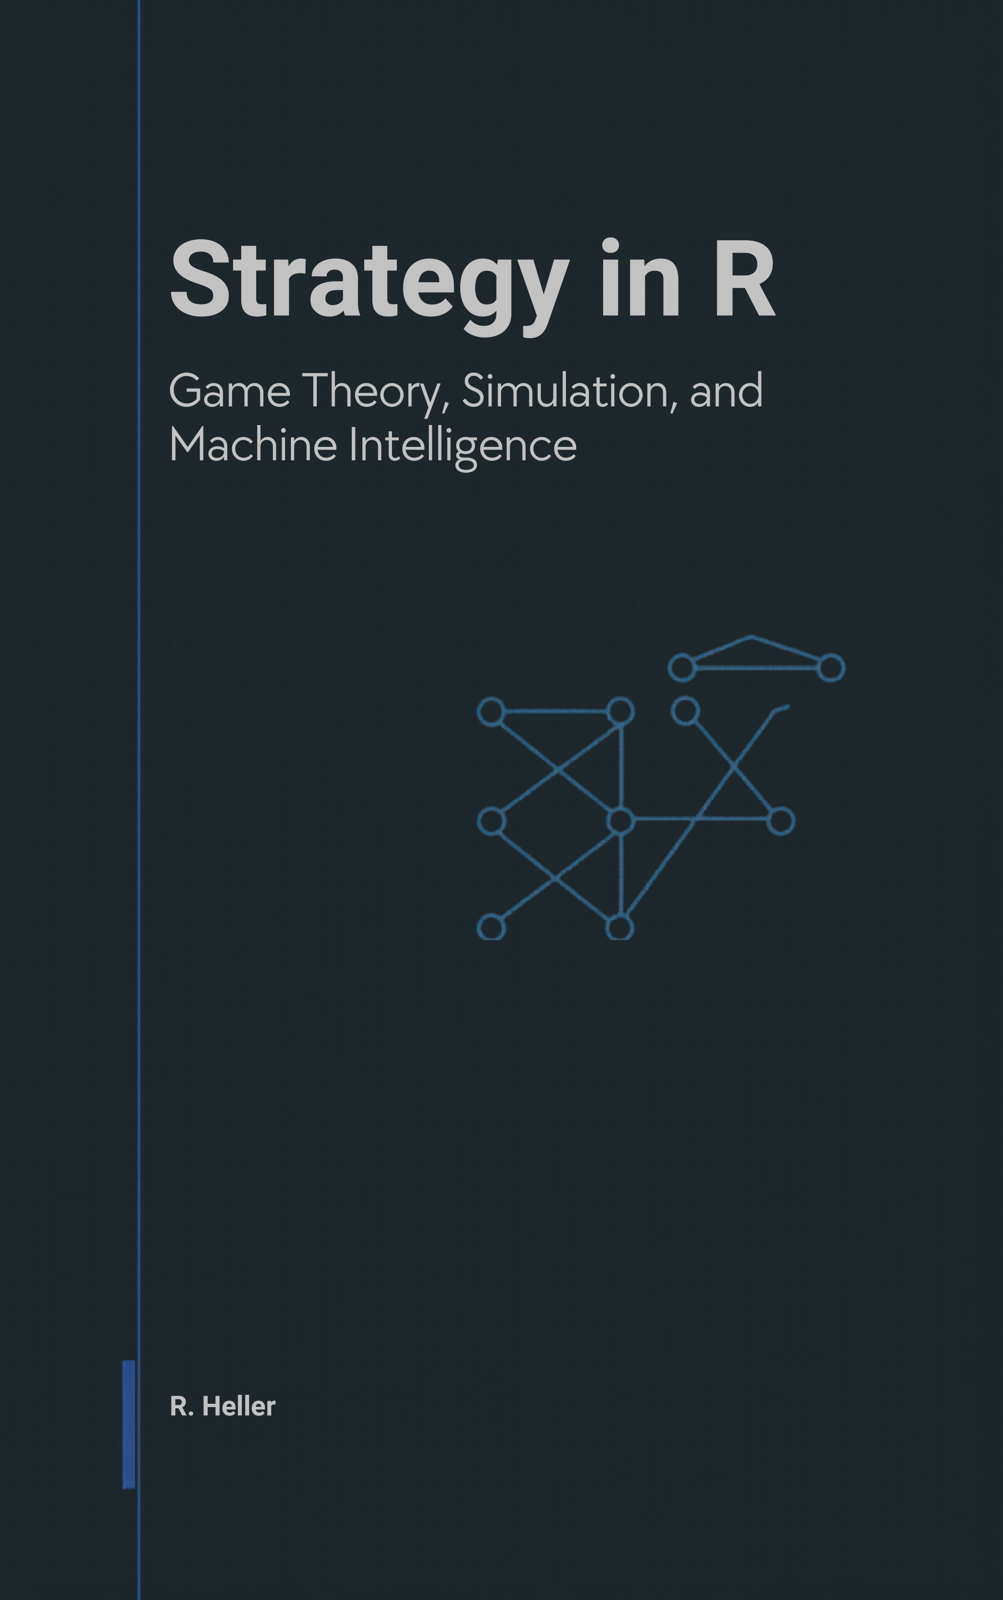
\includegraphics[width=0.4\linewidth,alt={Strategy in R cover}]{images/cover} \end{center}

\section*{About this book}\label{about-this-book}
\addcontentsline{toc}{section}{About this book}

\emph{Strategy in R} brings two ideas together: the formal language of game theory and the practical computation that makes it tractable. Part I builds the foundations from scratch --- normal- and extensive-form games, Nash equilibrium, mixed strategies, Bayesian games, repeated games, and cooperative game theory. Part II tours the R toolkit (\texttt{GameTheory}, \texttt{CoopGame}, \texttt{gtree}, \texttt{nashpy} via \texttt{reticulate}, custom solvers).

Parts III and IV move into simulation and AI: Monte Carlo methods, agent-based models, Axelrod's tournament, replicator dynamics, evolutionarily stable strategies, network games, performance with Rcpp, then reinforcement learning, multi-agent RL, self-play and AlphaZero, counterfactual regret minimisation, GANs as minimax games, and LLM agents.

Parts V and VI close with applications (auctions, mechanism design, matching markets, bargaining, empirical case studies) and a section on ethics and the future of strategic AI.

The book is for graduate students, researchers, and practitioners with working R fluency who want to apply it to strategic interaction. It assumes no prior game-theory background. It is not a pure-mathematics textbook, not a general machine-learning textbook, and not a software-engineering manual.

\section*{How to use this book}\label{how-to-use-this-book}
\addcontentsline{toc}{section}{How to use this book}

\begin{itemize}
\tightlist
\item
  \textbf{Reading paths.} Front-to-back works; theorists can skim Parts II--IV; R programmers can dip into Parts II--IV and refer back to Part I as needed.
\item
  \textbf{Code lives} under \texttt{R/} (helpers, theme, solvers) and \texttt{python/} (CFR, deep RL via \texttt{reticulate}); example data under \texttt{data/}. Every chapter is rebuildable in isolation: \texttt{bookdown::preview\_chapter("12-gtree-package.Rmd")}.
\item
  \textbf{Per-chapter PDF.} Every chapter page has a ``⬇ Download this chapter (PDF)'' button in the top-right.
\item
  \textbf{Whole-book downloads.} The PDF and EPUB are linked from the navbar's Download menu.
\item
  \textbf{Corrections and suggestions} go to the \href{https://github.com/r-heller/strategy-in-r/issues}{issue tracker}.
\end{itemize}

\section*{License}\label{license}
\addcontentsline{toc}{section}{License}

The content of this book is released under the \href{https://creativecommons.org/licenses/by/4.0/}{Creative Commons Attribution 4.0 International License} (see \href{https://github.com/r-heller/strategy-in-r/blob/main/LICENSE-CONTENT}{\texttt{LICENSE-CONTENT}}). Source code is released under the \href{https://opensource.org/licenses/MIT}{MIT License}.

\section*{Citing this Guide}\label{citing-this-guide}
\addcontentsline{toc}{section}{Citing this Guide}

The suggested citation is:

\begin{boxempty}
\textbf{Heller, R.} (2026). \emph{Strategy in R: Game Theory,
Simulation, and Machine Intelligence} (Version v0.1.0). Self-published
via GitHub Pages. \url{https://r-heller.github.io/strategy-in-r/}.
\end{boxempty}

Download the reference as \href{citation-files/citation.bib}{BibTeX} or \href{citation-files/citation.ris}{RIS}.

\chapter*{Impressum}\label{impressum}
\addcontentsline{toc}{chapter}{Impressum}

\textbf{Strategy in R: Game Theory, Simulation, and Machine Intelligence}

© 2026 Raban Heller. ORCID: \href{https://orcid.org/0000-0001-8006-9742}{0000-0001-8006-9742}.

Content released under the \href{https://creativecommons.org/licenses/by/4.0/}{Creative Commons Attribution 4.0 International License} (CC BY 4.0).

Source code released under the \href{https://opensource.org/licenses/MIT}{MIT License}.

Published online: \url{https://r-heller.github.io/strategy-in-r/}
Source repository: \url{https://github.com/r-heller/strategy-in-r}

Version: v0.1.0 · Build date: 2026-05-12

\section*{Suggested citation}\label{suggested-citation}
\addcontentsline{toc}{section}{Suggested citation}

\begin{quote}
Heller, R. (2026). \emph{Strategy in R: Game Theory, Simulation, and Machine Intelligence} (Version v0.1.0). \url{https://r-heller.github.io/strategy-in-r/}.
\end{quote}

\section*{Disclaimer}\label{disclaimer}
\addcontentsline{toc}{section}{Disclaimer}

This book is provided ``as is'' without warranty of any kind. The author assumes no responsibility for errors or omissions.

\section*{Contact}\label{contact}
\addcontentsline{toc}{section}{Contact}

For corrections, suggestions, or issues: \url{https://github.com/r-heller/strategy-in-r/issues}

\chapter*{How to use this book}\label{how-to-use-this-book-1}
\addcontentsline{toc}{chapter}{How to use this book}

\section*{Reading paths}\label{reading-paths}
\addcontentsline{toc}{section}{Reading paths}

\begin{itemize}
\tightlist
\item
  \textbf{Linear} --- front-to-back; expects no prior game-theory background.
\item
  \textbf{Theorist} --- Part I → Part V (applications) → Part VI (ethics); skim Parts II--IV for tools.
\item
  \textbf{R programmer} --- Part II (toolkit) → Part III (simulation) → dip into Part IV (AI/ML); refer to Part I as a reference.
\item
  \textbf{AI researcher} --- Part IV → Part VI; treat Part I as a glossary.
\end{itemize}

\section*{Chapter conventions}\label{chapter-conventions}
\addcontentsline{toc}{section}{Chapter conventions}

\begin{itemize}
\tightlist
\item
  Each chapter opens with a concrete question, not a definition.
\item
  Code is shown in full; outputs follow immediately; interpretation is a separate paragraph.
\item
  Cross-references use bookdown's \texttt{\textbackslash{}@ref()} syntax: \texttt{Chapter\ \textbackslash{}@ref(sec-nash-equilibrium)}, \texttt{Figure\ \textbackslash{}@ref(fig:axelrod-ranking)}, \texttt{Table\ \textbackslash{}@ref(tab:auction-types)}.
\item
  Exercises live at the end of each chapter; solutions are in Appendix D.
\end{itemize}

\section*{Companion code and data}\label{companion-code-and-data}
\addcontentsline{toc}{section}{Companion code and data}

\begin{itemize}
\tightlist
\item
  All R scripts live under \texttt{R/}; example datasets under \texttt{data/}; Python helpers under \texttt{python/}.
\item
  Every chapter is rebuildable in isolation: \texttt{bookdown::preview\_chapter("12-gtree-package.Rmd")}.
\end{itemize}

\section*{Downloads}\label{downloads}
\addcontentsline{toc}{section}{Downloads}

\begin{itemize}
\tightlist
\item
  A whole-book PDF and EPUB are linked from the navbar.
\item
  Each chapter page has a per-chapter PDF download in the top-right.
\end{itemize}

\section*{How to cite}\label{how-to-cite}
\addcontentsline{toc}{section}{How to cite}

See the \emph{Impressum} for the suggested citation, and \texttt{citation.bib} in the repository for a BibTeX entry.

\chapter*{Notation}\label{notation}
\addcontentsline{toc}{chapter}{Notation}

{\def\LTcaptype{none} % do not increment counter
\begin{longtable}[]{@{}
  >{\raggedright\arraybackslash}p{(\linewidth - 2\tabcolsep) * \real{0.4706}}
  >{\raggedright\arraybackslash}p{(\linewidth - 2\tabcolsep) * \real{0.5294}}@{}}
\toprule\noalign{}
\begin{minipage}[b]{\linewidth}\raggedright
Symbol
\end{minipage} & \begin{minipage}[b]{\linewidth}\raggedright
Meaning
\end{minipage} \\
\midrule\noalign{}
\endhead
\bottomrule\noalign{}
\endlastfoot
\(N\) & Set of players, \(N = \{1, 2, \dots, n\}\) \\
\(A_i\) & Action set of player \(i\) \\
\(A = \prod_i A_i\) & Joint action space \\
\(a_{-i}\) & Action profile of all players except \(i\) \\
\(u_i : A \to \mathbb{R}\) & Payoff (utility) function of player \(i\) \\
\(\sigma_i \in \Delta(A_i)\) & Mixed strategy of player \(i\) \\
\$\sigma\^{}* \$ & Nash equilibrium profile \\
\(v(S)\) & Characteristic function of coalition \(S\) in cooperative games \\
\(\phi_i(v)\) & Shapley value of player \(i\) \\
\(\pi\) & Policy in reinforcement learning \\
\(Q(s,a)\) & Action--value function \\
\(\gamma\) & Discount factor \\
\(\mathbb{E}[\cdot]\) & Expectation \\
\end{longtable}
}

\section*{Common abbreviations}\label{common-abbreviations}
\addcontentsline{toc}{section}{Common abbreviations}

{\def\LTcaptype{none} % do not increment counter
\begin{longtable}[]{@{}ll@{}}
\toprule\noalign{}
Abbrev. & Expansion \\
\midrule\noalign{}
\endhead
\bottomrule\noalign{}
\endlastfoot
BR & Best response \\
BNE & Bayesian Nash equilibrium \\
CFR & Counterfactual regret minimisation \\
ESS & Evolutionarily stable strategy \\
MARL & Multi-agent reinforcement learning \\
MDP & Markov decision process \\
MSNE & Mixed-strategy Nash equilibrium \\
NE & Nash equilibrium \\
PD & Prisoner's dilemma \\
RL & Reinforcement learning \\
SPE & Subgame-perfect equilibrium \\
TU / NTU & Transferable / non-transferable utility \\
VCG & Vickrey--Clarke--Groves mechanism \\
\end{longtable}
}

\chapter{Introduction}\label{sec-introduction}

\begin{quote}
Why study strategic interaction computationally, and why R is the right tool for the job.
\#\# The computational turn in game theory
\end{quote}

Game theory began as a branch of mathematics. Von Neumann and Morgenstern (\citeproc{ref-von-neumann1944}{1944}) laid the foundations; Nash (\citeproc{ref-nash1950}{1950}) proved that every finite game has an equilibrium. For decades, the field advanced primarily through theorems and proofs.

But the questions that matter most --- \emph{Which equilibrium will players actually reach? How do strategies evolve in populations? Can machines learn to play well?} --- are fundamentally computational questions. They require simulation, numerical methods, and algorithm design. This book is about answering those questions with working code.

\section{Why R?}\label{why-r}

R is the lingua franca of statistical computing and data science. It has mature ecosystems for visualization (\texttt{ggplot2}), data manipulation (\texttt{dplyr}), differential equations (\texttt{deSolve}), network analysis (\texttt{igraph}), and interactive graphics (\texttt{plotly}). For researchers who already think in R, there is no reason to context-switch to another language for game-theoretic computation.

Where R falls short --- deep learning, counterfactual regret minimization --- we use Python via \texttt{reticulate}, keeping the analysis pipeline in R while calling specialized Python libraries.

\section{The structure of this book}\label{the-structure-of-this-book}

The six parts of this book form a progression:

\begin{enumerate}
\def\labelenumi{\arabic{enumi}.}
\tightlist
\item
  \textbf{Foundations} build the conceptual vocabulary: what games are, how to solve them, what equilibrium means.
\item
  \textbf{The R Toolkit} introduces the packages and utilities we use throughout.
\item
  \textbf{Simulation} moves from analytical solutions to computational experiments: Monte Carlo, agent-based models, evolutionary dynamics.
\item
  \textbf{AI and Machine Learning} explores how learning agents interact strategically: reinforcement learning, self-play, and frontier methods.
\item
  \textbf{Applications} grounds the theory in real domains: auctions, matching markets, bargaining, and empirical case studies.
\item
  \textbf{Ethics and the Future} asks what happens when strategic AI systems interact with humans and each other.
\end{enumerate}

Each chapter is self-contained enough to read independently, but the parts are designed to be read in order for a coherent narrative.

\section{How to use this book}\label{how-to-use-this-book-2}

\textbf{Linear reading} is best for graduate courses or self-study in game theory with a computational focus. Start at Part I, Chapter 1.

\textbf{Reference reading} works well for practitioners who need a specific tool. Jump to the relevant chapter, follow cross-references backward for prerequisites.

\textbf{Project-based reading} pairs well with the exercises. Each chapter ends with problems that can serve as starting points for course projects or research extensions.

Let's begin.

\part{Part I --- Foundations of Game Theory}\label{part-part-i-foundations-of-game-theory}

\chapter{What is a Game?}\label{sec-what-is-a-game}

\begin{quote}
Players, actions, payoffs, and information --- the four building blocks that turn any strategic situation into a formal game. This chapter introduces the modeling stance of game theory, walks through canonical examples such as the Prisoner's Dilemma, coordination, and zero-sum games, and implements a reusable payoff-matrix visualization in R.
\end{quote}

\section*{Learning objectives}\label{learning-objectives}
\addcontentsline{toc}{section}{Learning objectives}

After completing this chapter you will be able to:

\begin{itemize}
\tightlist
\item
  Identify the four core ingredients of a game: players, actions, payoffs, and information.
\item
  Explain why a situation qualifies as a ``strategic interaction'' rather than a simple decision problem.
\item
  Represent a simultaneous-move game as a payoff matrix and interpret its entries.
\item
  Construct and visualize payoff matrices for classic 2x2 games in R.
\item
  Distinguish between zero-sum, coordination, and social-dilemma games by inspecting their payoff structure.
\end{itemize}

\section{Motivation}\label{motivation}

Imagine two coffee shops that open on the same street. Each owner must set a price without knowing the competitor's choice. The profit of each shop depends not only on its own price but also on the price set by the other. This mutual dependence is the hallmark of a \emph{strategic interaction}: the outcome for any one participant is shaped by the choices of all participants together.

Situations like this arise everywhere --- in economics, politics, biology, computer science, and everyday life. Firms compete on pricing and advertising; countries negotiate treaties; bacteria evolve resistance; autonomous vehicles coordinate at intersections. What unites these disparate settings is a common logical structure that can be captured by a single word: \emph{game}.

Game theory provides a precise mathematical language for reasoning about strategic interactions. It was launched by Neumann \& Morgenstern (\citeproc{ref-von-neumann1944}{1944}), who demonstrated that parlour games, market competition, and military tactics all share the same formal skeleton. A few years later, Nash (\citeproc{ref-nash1950}{1950}) showed that every finite game possesses at least one equilibrium --- a combination of strategies from which no player wants to deviate unilaterally. These two contributions created a discipline that now spans the social sciences, biology, and artificial intelligence.

This chapter lays the foundation for everything that follows. Before we can solve games, simulate tournaments, or train learning agents, we need a clear vocabulary for describing what a game \emph{is}.

\section{Theory}\label{theory}

\subsection{The four building blocks}\label{the-four-building-blocks}

Following Osborne (\citeproc{ref-osborne2004}{2004}), a game in \emph{strategic form} is defined by four elements:

\begin{enumerate}
\def\labelenumi{\arabic{enumi}.}
\item
  \textbf{Players.} A finite set \(N = \{1, 2, \ldots, n\}\) of decision-makers. Each player is assumed to be rational --- they have well-defined preferences and act to maximize their own payoff.
\item
  \textbf{Actions (strategies).} For each player \(i\), a set \(A_i\) of available choices. In a simultaneous-move game every player chooses an action without observing what the others do. The set of all action profiles is \(A = A_1 \times A_2 \times \cdots \times A_n\).
\item
  \textbf{Payoffs.} A function \(u_i : A \to \mathbb{R}\) that assigns a numerical reward to player \(i\) for every possible combination of actions. Payoffs encode preferences: player \(i\) prefers action profile \(a\) to profile \(a'\) if and only if \(u_i(a) > u_i(a')\).
\item
  \textbf{Information.} What each player knows when choosing an action. In a simultaneous game, players choose without observing others' moves; in a sequential game, later movers may observe earlier choices. We explore sequential information structures in \ref{sec-extensive-form}.
\end{enumerate}

A compact way to represent a two-player simultaneous game is the \emph{payoff matrix} (also called the \emph{normal form}). Each row corresponds to an action of Player 1, each column to an action of Player 2, and each cell contains a pair \((u_1, u_2)\) of payoffs. We study this representation in depth in \ref{sec-normal-form}.

\subsection{What makes a situation a ``game''?}\label{what-makes-a-situation-a-game}

Not every decision problem is a game. A hiker choosing a trail based on weather forecasts faces uncertainty, but the weather does not ``respond'' to the hiker's choice. A game requires at least two purposeful agents whose payoffs are mutually dependent. This \emph{interdependence} is the key criterion: if the best action for one player depends on the action chosen by another, the situation is strategic and thus a game (\citeproc{ref-shoham2009}{Shoham \& Leyton-Brown, 2009}).

\subsection{Three canonical examples}\label{three-canonical-examples}

\textbf{The Prisoner's Dilemma.} Two suspects are interrogated separately. Each can \emph{Cooperate} (stay silent) or \emph{Defect} (betray the other). Mutual cooperation yields a moderate reward for both, mutual defection yields a poor outcome for both, and unilateral defection gives the defector a high payoff at the cooperator's expense. The tragedy is that each player has a dominant incentive to defect, even though mutual cooperation would leave both better off. This game is central to the study of cooperation and is revisited in \ref{sec-repeated-games} and \ref{sec-axelrod-tournament}. The payoff structure is:

{\def\LTcaptype{none} % do not increment counter
\begin{longtable}[]{@{}lll@{}}
\toprule\noalign{}
& Cooperate & Defect \\
\midrule\noalign{}
\endhead
\bottomrule\noalign{}
\endlastfoot
\textbf{Cooperate} & (3, 3) & (0, 5) \\
\textbf{Defect} & (5, 0) & (1, 1) \\
\end{longtable}
}

\textbf{Coordination (Stag Hunt).} Two hunters can chase a \emph{Stag} (which requires joint effort) or a \emph{Hare} (which can be caught alone). If both hunt the stag, both feast; if one hunts alone, the stag escapes and that hunter gets nothing while the other catches a hare. The game has two pure-strategy equilibria and highlights the tension between efficiency and safety.

{\def\LTcaptype{none} % do not increment counter
\begin{longtable}[]{@{}lll@{}}
\toprule\noalign{}
& Stag & Hare \\
\midrule\noalign{}
\endhead
\bottomrule\noalign{}
\endlastfoot
\textbf{Stag} & (4, 4) & (0, 3) \\
\textbf{Hare} & (3, 0) & (2, 2) \\
\end{longtable}
}

\textbf{Zero-sum (Matching Pennies).} Each player secretly shows \emph{Heads} or \emph{Tails}. If the coins match, Player 1 wins; otherwise Player 2 wins. Every gain for one player is an equal loss for the other, so \(u_1(a) + u_2(a) = 0\) for every profile \(a\). This is the class of games Neumann \& Morgenstern (\citeproc{ref-von-neumann1944}{1944}) first solved completely. We study mixed-strategy solutions in \ref{sec-mixed-strategies}.

{\def\LTcaptype{none} % do not increment counter
\begin{longtable}[]{@{}lll@{}}
\toprule\noalign{}
& Heads & Tails \\
\midrule\noalign{}
\endhead
\bottomrule\noalign{}
\endlastfoot
\textbf{Heads} & (1, -1) & (-1, 1) \\
\textbf{Tails} & (-1, 1) & (1, -1) \\
\end{longtable}
}

\section{Implementation in R}\label{implementation-in-r}

We now build an R function to create and visualize any 2x2 payoff matrix. The function returns a tidy data frame suitable for plotting with \texttt{ggplot2}.

\begin{Shaded}
\begin{Highlighting}[]
\CommentTok{\# Build a tidy data frame for a 2x2 payoff matrix}
\NormalTok{make\_payoff\_df }\OtherTok{\textless{}{-}} \ControlFlowTok{function}\NormalTok{(game\_name, row\_actions, col\_actions, payoffs) \{}
  \CommentTok{\# payoffs: list of four pairs c(u1, u2) in row{-}major order}
  \FunctionTok{tibble}\NormalTok{(}
    \AttributeTok{game       =}\NormalTok{ game\_name,}
    \AttributeTok{row\_action =} \FunctionTok{rep}\NormalTok{(row\_actions, }\AttributeTok{each =} \FunctionTok{length}\NormalTok{(col\_actions)),}
    \AttributeTok{col\_action =} \FunctionTok{rep}\NormalTok{(col\_actions, }\AttributeTok{times =} \FunctionTok{length}\NormalTok{(row\_actions)),}
    \AttributeTok{payoff\_1   =} \FunctionTok{map\_dbl}\NormalTok{(payoffs, }\DecValTok{1}\NormalTok{),}
    \AttributeTok{payoff\_2   =} \FunctionTok{map\_dbl}\NormalTok{(payoffs, }\DecValTok{2}\NormalTok{),}
    \AttributeTok{label      =} \FunctionTok{glue}\NormalTok{(}\StringTok{"(\{payoff\_1\}, \{payoff\_2\})"}\NormalTok{)}
\NormalTok{  )}
\NormalTok{\}}
\end{Highlighting}
\end{Shaded}

Next we build data frames for our three canonical games and combine them into one tidy dataset.

\begin{Shaded}
\begin{Highlighting}[]
\NormalTok{pd }\OtherTok{\textless{}{-}} \FunctionTok{make\_payoff\_df}\NormalTok{(}
  \StringTok{"Prisoner\textquotesingle{}s Dilemma"}\NormalTok{,}
  \FunctionTok{c}\NormalTok{(}\StringTok{"Cooperate"}\NormalTok{, }\StringTok{"Defect"}\NormalTok{), }\FunctionTok{c}\NormalTok{(}\StringTok{"Cooperate"}\NormalTok{, }\StringTok{"Defect"}\NormalTok{),}
  \FunctionTok{list}\NormalTok{(}\FunctionTok{c}\NormalTok{(}\DecValTok{3}\NormalTok{, }\DecValTok{3}\NormalTok{), }\FunctionTok{c}\NormalTok{(}\DecValTok{0}\NormalTok{, }\DecValTok{5}\NormalTok{), }\FunctionTok{c}\NormalTok{(}\DecValTok{5}\NormalTok{, }\DecValTok{0}\NormalTok{), }\FunctionTok{c}\NormalTok{(}\DecValTok{1}\NormalTok{, }\DecValTok{1}\NormalTok{))}
\NormalTok{)}

\NormalTok{stag }\OtherTok{\textless{}{-}} \FunctionTok{make\_payoff\_df}\NormalTok{(}
  \StringTok{"Stag Hunt"}\NormalTok{,}
  \FunctionTok{c}\NormalTok{(}\StringTok{"Stag"}\NormalTok{, }\StringTok{"Hare"}\NormalTok{), }\FunctionTok{c}\NormalTok{(}\StringTok{"Stag"}\NormalTok{, }\StringTok{"Hare"}\NormalTok{),}
  \FunctionTok{list}\NormalTok{(}\FunctionTok{c}\NormalTok{(}\DecValTok{4}\NormalTok{, }\DecValTok{4}\NormalTok{), }\FunctionTok{c}\NormalTok{(}\DecValTok{0}\NormalTok{, }\DecValTok{3}\NormalTok{), }\FunctionTok{c}\NormalTok{(}\DecValTok{3}\NormalTok{, }\DecValTok{0}\NormalTok{), }\FunctionTok{c}\NormalTok{(}\DecValTok{2}\NormalTok{, }\DecValTok{2}\NormalTok{))}
\NormalTok{)}

\NormalTok{mp }\OtherTok{\textless{}{-}} \FunctionTok{make\_payoff\_df}\NormalTok{(}
  \StringTok{"Matching Pennies"}\NormalTok{,}
  \FunctionTok{c}\NormalTok{(}\StringTok{"Heads"}\NormalTok{, }\StringTok{"Tails"}\NormalTok{), }\FunctionTok{c}\NormalTok{(}\StringTok{"Heads"}\NormalTok{, }\StringTok{"Tails"}\NormalTok{),}
  \FunctionTok{list}\NormalTok{(}\FunctionTok{c}\NormalTok{(}\DecValTok{1}\NormalTok{, }\SpecialCharTok{{-}}\DecValTok{1}\NormalTok{), }\FunctionTok{c}\NormalTok{(}\SpecialCharTok{{-}}\DecValTok{1}\NormalTok{, }\DecValTok{1}\NormalTok{), }\FunctionTok{c}\NormalTok{(}\SpecialCharTok{{-}}\DecValTok{1}\NormalTok{, }\DecValTok{1}\NormalTok{), }\FunctionTok{c}\NormalTok{(}\DecValTok{1}\NormalTok{, }\SpecialCharTok{{-}}\DecValTok{1}\NormalTok{))}
\NormalTok{)}

\NormalTok{games }\OtherTok{\textless{}{-}} \FunctionTok{bind\_rows}\NormalTok{(pd, stag, mp) }\SpecialCharTok{|\textgreater{}}
  \FunctionTok{mutate}\NormalTok{(}
    \AttributeTok{game =} \FunctionTok{factor}\NormalTok{(game, }\AttributeTok{levels =} \FunctionTok{c}\NormalTok{(}\StringTok{"Prisoner\textquotesingle{}s Dilemma"}\NormalTok{,}
                                   \StringTok{"Stag Hunt"}\NormalTok{,}
                                   \StringTok{"Matching Pennies"}\NormalTok{))}
\NormalTok{  )}
\end{Highlighting}
\end{Shaded}

Now we produce a publication-quality heatmap of the three payoff matrices, using Player 1's payoff for the fill colour.

\begin{Shaded}
\begin{Highlighting}[]
\NormalTok{p\_heatmap }\OtherTok{\textless{}{-}} \FunctionTok{ggplot}\NormalTok{(games, }\FunctionTok{aes}\NormalTok{(}\AttributeTok{x =}\NormalTok{ col\_action, }\AttributeTok{y =}\NormalTok{ row\_action,}
                                \AttributeTok{fill =}\NormalTok{ payoff\_1)) }\SpecialCharTok{+}
  \FunctionTok{geom\_tile}\NormalTok{(}\AttributeTok{colour =} \StringTok{"white"}\NormalTok{, }\AttributeTok{linewidth =} \FloatTok{1.2}\NormalTok{) }\SpecialCharTok{+}
  \FunctionTok{geom\_text}\NormalTok{(}\FunctionTok{aes}\NormalTok{(}\AttributeTok{label =}\NormalTok{ label), }\AttributeTok{size =} \FloatTok{3.6}\NormalTok{, }\AttributeTok{fontface =} \StringTok{"bold"}\NormalTok{) }\SpecialCharTok{+}
  \FunctionTok{facet\_wrap}\NormalTok{(}\SpecialCharTok{\textasciitilde{}}\NormalTok{ game, }\AttributeTok{scales =} \StringTok{"free"}\NormalTok{) }\SpecialCharTok{+}
  \FunctionTok{scale\_fill\_gradient2}\NormalTok{(}
    \AttributeTok{low =}\NormalTok{ okabe\_ito[}\DecValTok{6}\NormalTok{],   }\CommentTok{\# vermillion for negative/low}
    \AttributeTok{mid =} \StringTok{"white"}\NormalTok{,}
    \AttributeTok{high =}\NormalTok{ okabe\_ito[}\DecValTok{3}\NormalTok{],  }\CommentTok{\# bluish{-}green for positive/high}
    \AttributeTok{midpoint =} \FloatTok{1.5}\NormalTok{,}
    \AttributeTok{name =} \StringTok{"Player 1}\SpecialCharTok{\textbackslash{}n}\StringTok{payoff"}
\NormalTok{  ) }\SpecialCharTok{+}
  \FunctionTok{scale\_y\_discrete}\NormalTok{(}\AttributeTok{limits =}\NormalTok{ rev) }\SpecialCharTok{+}
  \FunctionTok{labs}\NormalTok{(}\AttributeTok{x =} \StringTok{"Player 2"}\NormalTok{, }\AttributeTok{y =} \StringTok{"Player 1"}\NormalTok{) }\SpecialCharTok{+}
  \FunctionTok{theme\_publication}\NormalTok{(}\AttributeTok{base\_size =} \DecValTok{11}\NormalTok{) }\SpecialCharTok{+}
  \FunctionTok{theme}\NormalTok{(}
    \AttributeTok{strip.text =} \FunctionTok{element\_text}\NormalTok{(}\AttributeTok{face =} \StringTok{"bold"}\NormalTok{, }\AttributeTok{size =} \DecValTok{11}\NormalTok{),}
    \AttributeTok{panel.grid =} \FunctionTok{element\_blank}\NormalTok{(),}
    \AttributeTok{axis.ticks =} \FunctionTok{element\_blank}\NormalTok{()}
\NormalTok{  )}

\NormalTok{p\_heatmap}
\end{Highlighting}
\end{Shaded}

\begin{figure}

{\centering 
\includegraphics[width=0.8\linewidth]{01-what-is-a-game_files/figure-latex/payoff-heatmap-1} 

}

\caption{Payoff matrices for three canonical 2x2 games. Cell colour encodes Player 1's payoff using a diverging Okabe-Ito-inspired palette; each cell displays both players' payoffs as an ordered pair.}\label{fig:payoff-heatmap}
\end{figure}

\section{Worked example}\label{worked-example}

Let us walk through the Prisoner's Dilemma step by step to cement the vocabulary.

\textbf{Step 1 --- Identify the players.} There are two players: Suspect 1 and Suspect 2.

\textbf{Step 2 --- List the actions.} Each player can \emph{Cooperate} (stay silent) or \emph{Defect} (betray). So \(A_1 = A_2 = \{\text{Cooperate}, \text{Defect}\}\).

\textbf{Step 3 --- Specify payoffs.} We read the matrix row by row:

\begin{Shaded}
\begin{Highlighting}[]
\NormalTok{pd }\SpecialCharTok{|\textgreater{}}
  \FunctionTok{select}\NormalTok{(}
    \StringTok{\textasciigrave{}}\AttributeTok{Player 1}\StringTok{\textasciigrave{}} \OtherTok{=}\NormalTok{ row\_action,}
    \StringTok{\textasciigrave{}}\AttributeTok{Player 2}\StringTok{\textasciigrave{}} \OtherTok{=}\NormalTok{ col\_action,}
    \StringTok{\textasciigrave{}}\AttributeTok{Payoff 1}\StringTok{\textasciigrave{}}  \OtherTok{=}\NormalTok{ payoff\_1,}
    \StringTok{\textasciigrave{}}\AttributeTok{Payoff 2}\StringTok{\textasciigrave{}}  \OtherTok{=}\NormalTok{ payoff\_2}
\NormalTok{  ) }\SpecialCharTok{|\textgreater{}}
  \FunctionTok{gt}\NormalTok{() }\SpecialCharTok{|\textgreater{}}
  \FunctionTok{tab\_header}\NormalTok{(}\AttributeTok{title =} \StringTok{"Prisoner\textquotesingle{}s Dilemma Payoffs"}\NormalTok{) }\SpecialCharTok{|\textgreater{}}
  \FunctionTok{cols\_align}\NormalTok{(}\AttributeTok{align =} \StringTok{"center"}\NormalTok{)}
\end{Highlighting}
\end{Shaded}

\begin{table}[t]
\caption*{
{\fontsize{20}{25}\selectfont  Prisoner's Dilemma Payoffs\fontsize{12}{15}\selectfont }
} 
\fontsize{12.0pt}{14.0pt}\selectfont
\begin{tabular*}{\linewidth}{@{\extracolsep{\fill}}cccc}
\toprule
Player 1 & Player 2 & Payoff 1 & Payoff 2 \\ 
\midrule\addlinespace[2.5pt]
Cooperate & Cooperate & 3 & 3 \\ 
Cooperate & Defect & 0 & 5 \\ 
Defect & Cooperate & 5 & 0 \\ 
Defect & Defect & 1 & 1 \\ 
\bottomrule
\end{tabular*}
\end{table}

\textbf{Step 4 --- Check for dominance.} Regardless of what Player 2 does, Player 1 earns more by defecting (5 \textgreater{} 3 when Player 2 cooperates; 1 \textgreater{} 0 when Player 2 defects). Defect is a \emph{dominant strategy} for Player 1. By symmetry, the same holds for Player 2.

\textbf{Step 5 --- Identify the outcome.} Both players defect, yielding payoffs (1, 1). This is the unique Nash equilibrium, yet both players would prefer mutual cooperation at (3, 3). The gap between individual rationality and collective welfare is what makes the Prisoner's Dilemma so compelling --- and why mechanisms for sustaining cooperation, from repeated interaction (\citeproc{ref-axelrod1981}{Axelrod, 1981}) to enforceable contracts, are among the central concerns of game theory.

\section{Extensions}\label{extensions}

The four-element definition introduced here is deliberately minimal. Real-world strategic situations often involve richer structure:

\begin{itemize}
\tightlist
\item
  \textbf{Sequential moves and information sets.} When players move in turn and can observe some or all prior actions, we use the \emph{extensive form} --- a game tree that encodes timing and information. See \ref{sec-extensive-form}.
\item
  \textbf{Mixed strategies.} Players may randomize over actions. Neumann \& Morgenstern (\citeproc{ref-von-neumann1944}{1944}) proved that every finite zero-sum game has a value in mixed strategies; Nash (\citeproc{ref-nash1950}{1950}) extended the existence result to all finite games. We cover mixed strategies in \ref{sec-mixed-strategies}.
\item
  \textbf{Incomplete information.} When players are uncertain about others' payoffs or types, we enter the realm of \emph{Bayesian games}, treated in \ref{sec-bayesian-games}.
\item
  \textbf{Repeated interaction.} Many strategic encounters happen repeatedly. Repetition can sustain cooperation even in Prisoner's Dilemma settings, a theme explored in \ref{sec-repeated-games}.
\item
  \textbf{Multi-agent learning.} When agents learn from experience rather than computing equilibria analytically, game theory intersects with reinforcement learning (\citeproc{ref-sutton2018}{Sutton \& Barto, 2018}). We develop this connection in \ref{sec-q-learning} and \ref{sec-multi-agent-rl}.
\end{itemize}

The compact representation we built in R --- the \texttt{make\_payoff\_df()} function and heatmap visualization --- will be extended in \ref{sec-normal-form} where we study dominance, best responses, and iterated elimination of dominated strategies.

\section*{Exercises}\label{exercises}
\addcontentsline{toc}{section}{Exercises}

\begin{enumerate}
\def\labelenumi{\arabic{enumi}.}
\item
  \textbf{Identifying game elements.} Consider an intersection where two autonomous vehicles arrive simultaneously. Each can \emph{Go} or \emph{Yield}. If both go, they crash (payoff -5 each). If both yield, they waste time (payoff 0 each). If one goes and the other yields, the goer saves time (payoff 3) and the yielder waits (payoff 1). Write down the four elements (players, actions, payoffs, information) and construct the 2x2 payoff matrix. What type of game is this (zero-sum, coordination, or social dilemma)?
\item
  \textbf{Payoff heatmap.} Using the \texttt{make\_payoff\_df()} function from this chapter, create a payoff matrix for the \emph{Battle of the Sexes} game: two players choose between \emph{Opera} and \emph{Football}. Both prefer to coordinate, but Player 1 prefers Opera (payoffs 3, 2 when both choose Opera) and Player 2 prefers Football (payoffs 2, 3 when both choose Football). Miscoordination yields (0, 0). Plot the heatmap and describe the payoff structure.
\item
  \textbf{Zero-sum verification.} Prove algebraically that Matching Pennies is zero-sum by showing \(u_1(a) + u_2(a) = 0\) for every action profile. Then modify the payoffs so that the game is \emph{not} zero-sum but still competitive (Player 1 prefers matching and Player 2 prefers mismatching). Plot both versions side by side using \texttt{facet\_wrap()}.
\item
  \textbf{From story to model.} Pick a real-world scenario (e.g., two countries deciding whether to impose tariffs, two students deciding how much effort to put into a group project, or two streaming services choosing content investment levels). Identify the players, actions, and a plausible payoff structure. Use \texttt{make\_payoff\_df()} to encode your game and produce the heatmap. Discuss whether the game resembles a Prisoner's Dilemma, coordination game, or something else.
\item
  \textbf{Reading the literature.} Read the first two pages of Nash (\citeproc{ref-nash1950}{1950}). In your own words, state Nash's definition of an equilibrium point. How does it relate to the concept of a dominant-strategy outcome in the Prisoner's Dilemma?
\end{enumerate}

Solutions appear in \ref{sec-solutions}.

\chapter{Normal-Form Games}\label{sec-normal-form}

\begin{quote}
The normal (strategic) form is the workhorse representation of simultaneous-move games. This chapter introduces payoff matrices, strict and weak dominance, iterated elimination of strictly dominated strategies (IESDS), and the four classic 2x2 games that recur throughout game theory.
\end{quote}

\section*{Learning objectives}\label{learning-objectives-1}
\addcontentsline{toc}{section}{Learning objectives}

\begin{itemize}
\tightlist
\item
  Represent a simultaneous-move game as a payoff matrix and interpret its entries.
\item
  Distinguish strict dominance from weak dominance and identify dominated strategies.
\item
  Apply iterated elimination of strictly dominated strategies (IESDS) to simplify games.
\item
  Recognise and classify the four classic 2x2 games: Prisoner's Dilemma, Stag Hunt, Chicken, and Battle of the Sexes.
\item
  Implement payoff matrices and dominance checks in R and produce publication-quality figures.
\end{itemize}

\section{Motivation}\label{motivation-1}

Imagine two rival coffee shops opening on the same street, each choosing a price for their latte -- high or low -- without knowing the other's decision. Each shop's profit depends not only on its own price but also on the competitor's. If both charge high prices, they share a comfortable market; if one undercuts the other, the cheaper shop captures most customers; if both go low, margins evaporate for everyone.

This kind of simultaneous decision under strategic interdependence is exactly what the \textbf{normal-form} (or \textbf{strategic-form}) representation was designed to capture. Introduced by Neumann \& Morgenstern (\citeproc{ref-von-neumann1944}{1944}), the normal form strips a game down to its essentials: who are the players, what can each player do, and what payoff does each combination of choices produce? These elements are arranged in a \textbf{payoff matrix}, which makes the strategic structure visible at a glance and is the starting point for almost every solution concept in non-cooperative game theory.

\section{Theory}\label{theory-1}

\subsection{The normal-form representation}\label{the-normal-form-representation}

A finite \textbf{normal-form game} is a tuple \(G = (N, (S_i)_{i \in N}, (u_i)_{i \in N})\) where

\begin{itemize}
\tightlist
\item
  \(N = \{1, 2, \ldots, n\}\) is the set of \textbf{players},
\item
  \(S_i\) is the finite set of \textbf{strategies} (or actions) available to player \(i\), and
\item
  \(u_i : S_1 \times \cdots \times S_n \to \mathbb{R}\) is player \(i\)'s \textbf{payoff function}.
\end{itemize}

For a two-player game where Player 1 has \(m\) strategies and Player 2 has \(k\) strategies, we arrange payoffs in an \(m \times k\) matrix. Each cell \((i, j)\) contains the pair \((u_1(s_i, s_j),\; u_2(s_i, s_j))\). Player 1 chooses a row, Player 2 chooses a column, and the cell at their intersection determines both payoffs.

\subsection{Dominance}\label{dominance}

A strategy \(s_i\) \textbf{strictly dominates} another strategy \(s_i'\) if it yields a strictly higher payoff against \emph{every} possible strategy profile of the opponents:

\begin{equation}
u_i(s_i, s_{-i}) > u_i(s_i', s_{-i}) \quad \forall\; s_{-i} \in S_{-i}
\label{eq:strict-dom}
\end{equation}

A rational player will never play a strictly dominated strategy -- there is always something better, regardless of what others do.

A strategy \(s_i\) \textbf{weakly dominates} \(s_i'\) if it does at least as well against all opponent profiles and strictly better against at least one:

\begin{equation}
u_i(s_i, s_{-i}) \geq u_i(s_i', s_{-i}) \quad \forall\; s_{-i}, \qquad \text{with strict inequality for some } s_{-i}.
\label{eq:weak-dom}
\end{equation}

Weak dominance is a less decisive criterion: eliminating weakly dominated strategies can change the set of Nash equilibria and the order of elimination may matter, so it must be applied with care.

\subsection{Iterated elimination of strictly dominated strategies (IESDS)}\label{iterated-elimination-of-strictly-dominated-strategies-iesds}

If a strategy is strictly dominated, a rational player will never use it. Knowing this, the other players can remove that strategy from consideration, potentially revealing new dominated strategies in the reduced game. Repeating this process is called \textbf{IESDS} (iterated elimination of strictly dominated strategies).

A key property of IESDS is \textbf{order independence}: the final set of surviving strategies is the same regardless of the order in which dominated strategies are removed (\citeproc{ref-osborne2004}{Osborne, 2004, Chapter 2}). If IESDS reduces the game to a single strategy profile, the game is \textbf{dominance solvable} -- the Prisoner's Dilemma is the most famous example.

\subsection{Classic 2x2 games}\label{classic-2x2-games}

Four canonical 2x2 games appear throughout game theory and its applications. Each represents a different type of strategic tension:

\begin{itemize}
\tightlist
\item
  \textbf{Prisoner's Dilemma.} Each player has a dominant strategy (Defect), but mutual cooperation would make both better off. The unique Nash equilibrium is Pareto-inefficient.
\item
  \textbf{Stag Hunt.} Two pure-strategy equilibria exist: one payoff-dominant (both hunt Stag) and one risk-dominant (both hunt Hare). The game models the trade-off between trust and safety.
\item
  \textbf{Chicken (Hawk-Dove).} Two asymmetric pure equilibria (one swerves, the other does not) plus a mixed equilibrium. It captures brinkmanship and anti-coordination.
\item
  \textbf{Battle of the Sexes.} Two pure equilibria where players coordinate on different preferred outcomes, plus a mixed equilibrium. It models coordination with conflicting preferences.
\end{itemize}

These games reappear in \ref{sec-nash-equilibrium} for equilibrium analysis, in \ref{sec-mixed-strategies} for mixed-strategy computation, and in \ref{sec-repeated-games} for the study of cooperation over time.

\section{Implementation in R}\label{implementation-in-r-1}

We begin by building payoff matrices for the four classic games and writing a helper function to check for strictly dominated strategies.

\begin{Shaded}
\begin{Highlighting}[]
\CommentTok{\# Define the four classic 2x2 games as named lists}
\CommentTok{\# Each entry: list(A = Player 1 payoffs, B = Player 2 payoffs)}
\NormalTok{classic\_games }\OtherTok{\textless{}{-}} \FunctionTok{list}\NormalTok{(}
  \StringTok{"Prisoner\textquotesingle{}s Dilemma"} \OtherTok{=} \FunctionTok{list}\NormalTok{(}
    \AttributeTok{A =} \FunctionTok{matrix}\NormalTok{(}\FunctionTok{c}\NormalTok{(}\DecValTok{3}\NormalTok{, }\DecValTok{0}\NormalTok{, }\DecValTok{5}\NormalTok{, }\DecValTok{1}\NormalTok{), }\AttributeTok{nrow =} \DecValTok{2}\NormalTok{, }\AttributeTok{byrow =} \ConstantTok{TRUE}\NormalTok{,}
               \AttributeTok{dimnames =} \FunctionTok{list}\NormalTok{(}\FunctionTok{c}\NormalTok{(}\StringTok{"C"}\NormalTok{, }\StringTok{"D"}\NormalTok{), }\FunctionTok{c}\NormalTok{(}\StringTok{"C"}\NormalTok{, }\StringTok{"D"}\NormalTok{))),}
    \AttributeTok{B =} \FunctionTok{matrix}\NormalTok{(}\FunctionTok{c}\NormalTok{(}\DecValTok{3}\NormalTok{, }\DecValTok{5}\NormalTok{, }\DecValTok{0}\NormalTok{, }\DecValTok{1}\NormalTok{), }\AttributeTok{nrow =} \DecValTok{2}\NormalTok{, }\AttributeTok{byrow =} \ConstantTok{TRUE}\NormalTok{,}
               \AttributeTok{dimnames =} \FunctionTok{list}\NormalTok{(}\FunctionTok{c}\NormalTok{(}\StringTok{"C"}\NormalTok{, }\StringTok{"D"}\NormalTok{), }\FunctionTok{c}\NormalTok{(}\StringTok{"C"}\NormalTok{, }\StringTok{"D"}\NormalTok{)))}
\NormalTok{  ),}
  \StringTok{"Stag Hunt"} \OtherTok{=} \FunctionTok{list}\NormalTok{(}
    \AttributeTok{A =} \FunctionTok{matrix}\NormalTok{(}\FunctionTok{c}\NormalTok{(}\DecValTok{4}\NormalTok{, }\DecValTok{0}\NormalTok{, }\DecValTok{3}\NormalTok{, }\DecValTok{3}\NormalTok{), }\AttributeTok{nrow =} \DecValTok{2}\NormalTok{, }\AttributeTok{byrow =} \ConstantTok{TRUE}\NormalTok{,}
               \AttributeTok{dimnames =} \FunctionTok{list}\NormalTok{(}\FunctionTok{c}\NormalTok{(}\StringTok{"Stag"}\NormalTok{, }\StringTok{"Hare"}\NormalTok{), }\FunctionTok{c}\NormalTok{(}\StringTok{"Stag"}\NormalTok{, }\StringTok{"Hare"}\NormalTok{))),}
    \AttributeTok{B =} \FunctionTok{matrix}\NormalTok{(}\FunctionTok{c}\NormalTok{(}\DecValTok{4}\NormalTok{, }\DecValTok{3}\NormalTok{, }\DecValTok{0}\NormalTok{, }\DecValTok{3}\NormalTok{), }\AttributeTok{nrow =} \DecValTok{2}\NormalTok{, }\AttributeTok{byrow =} \ConstantTok{TRUE}\NormalTok{,}
               \AttributeTok{dimnames =} \FunctionTok{list}\NormalTok{(}\FunctionTok{c}\NormalTok{(}\StringTok{"Stag"}\NormalTok{, }\StringTok{"Hare"}\NormalTok{), }\FunctionTok{c}\NormalTok{(}\StringTok{"Stag"}\NormalTok{, }\StringTok{"Hare"}\NormalTok{)))}
\NormalTok{  ),}
  \StringTok{"Chicken"} \OtherTok{=} \FunctionTok{list}\NormalTok{(}
    \AttributeTok{A =} \FunctionTok{matrix}\NormalTok{(}\FunctionTok{c}\NormalTok{(}\DecValTok{0}\NormalTok{, }\SpecialCharTok{{-}}\DecValTok{1}\NormalTok{, }\DecValTok{1}\NormalTok{, }\SpecialCharTok{{-}}\DecValTok{5}\NormalTok{), }\AttributeTok{nrow =} \DecValTok{2}\NormalTok{, }\AttributeTok{byrow =} \ConstantTok{TRUE}\NormalTok{,}
               \AttributeTok{dimnames =} \FunctionTok{list}\NormalTok{(}\FunctionTok{c}\NormalTok{(}\StringTok{"Swerve"}\NormalTok{, }\StringTok{"Straight"}\NormalTok{), }\FunctionTok{c}\NormalTok{(}\StringTok{"Swerve"}\NormalTok{, }\StringTok{"Straight"}\NormalTok{))),}
    \AttributeTok{B =} \FunctionTok{matrix}\NormalTok{(}\FunctionTok{c}\NormalTok{(}\DecValTok{0}\NormalTok{, }\DecValTok{1}\NormalTok{, }\SpecialCharTok{{-}}\DecValTok{1}\NormalTok{, }\SpecialCharTok{{-}}\DecValTok{5}\NormalTok{), }\AttributeTok{nrow =} \DecValTok{2}\NormalTok{, }\AttributeTok{byrow =} \ConstantTok{TRUE}\NormalTok{,}
               \AttributeTok{dimnames =} \FunctionTok{list}\NormalTok{(}\FunctionTok{c}\NormalTok{(}\StringTok{"Swerve"}\NormalTok{, }\StringTok{"Straight"}\NormalTok{), }\FunctionTok{c}\NormalTok{(}\StringTok{"Swerve"}\NormalTok{, }\StringTok{"Straight"}\NormalTok{)))}
\NormalTok{  ),}
  \StringTok{"Battle of the Sexes"} \OtherTok{=} \FunctionTok{list}\NormalTok{(}
    \AttributeTok{A =} \FunctionTok{matrix}\NormalTok{(}\FunctionTok{c}\NormalTok{(}\DecValTok{3}\NormalTok{, }\DecValTok{0}\NormalTok{, }\DecValTok{0}\NormalTok{, }\DecValTok{2}\NormalTok{), }\AttributeTok{nrow =} \DecValTok{2}\NormalTok{, }\AttributeTok{byrow =} \ConstantTok{TRUE}\NormalTok{,}
               \AttributeTok{dimnames =} \FunctionTok{list}\NormalTok{(}\FunctionTok{c}\NormalTok{(}\StringTok{"Opera"}\NormalTok{, }\StringTok{"Football"}\NormalTok{), }\FunctionTok{c}\NormalTok{(}\StringTok{"Opera"}\NormalTok{, }\StringTok{"Football"}\NormalTok{))),}
    \AttributeTok{B =} \FunctionTok{matrix}\NormalTok{(}\FunctionTok{c}\NormalTok{(}\DecValTok{2}\NormalTok{, }\DecValTok{0}\NormalTok{, }\DecValTok{0}\NormalTok{, }\DecValTok{3}\NormalTok{), }\AttributeTok{nrow =} \DecValTok{2}\NormalTok{, }\AttributeTok{byrow =} \ConstantTok{TRUE}\NormalTok{,}
               \AttributeTok{dimnames =} \FunctionTok{list}\NormalTok{(}\FunctionTok{c}\NormalTok{(}\StringTok{"Opera"}\NormalTok{, }\StringTok{"Football"}\NormalTok{), }\FunctionTok{c}\NormalTok{(}\StringTok{"Opera"}\NormalTok{, }\StringTok{"Football"}\NormalTok{)))}
\NormalTok{  )}
\NormalTok{)}
\end{Highlighting}
\end{Shaded}

\subsection{Checking for strict dominance}\label{checking-for-strict-dominance}

\begin{Shaded}
\begin{Highlighting}[]
\NormalTok{find\_strictly\_dominated }\OtherTok{\textless{}{-}} \ControlFlowTok{function}\NormalTok{(payoff\_matrix) \{}

\NormalTok{  n }\OtherTok{\textless{}{-}} \FunctionTok{nrow}\NormalTok{(payoff\_matrix)}
\NormalTok{  dominated }\OtherTok{\textless{}{-}} \FunctionTok{character}\NormalTok{(}\DecValTok{0}\NormalTok{)}
\NormalTok{  strats }\OtherTok{\textless{}{-}} \FunctionTok{rownames}\NormalTok{(payoff\_matrix)}
  \ControlFlowTok{for}\NormalTok{ (i }\ControlFlowTok{in} \FunctionTok{seq\_len}\NormalTok{(n)) \{}
    \ControlFlowTok{for}\NormalTok{ (j }\ControlFlowTok{in} \FunctionTok{seq\_len}\NormalTok{(n)) \{}
      \ControlFlowTok{if}\NormalTok{ (i }\SpecialCharTok{!=}\NormalTok{ j }\SpecialCharTok{\&\&} \FunctionTok{all}\NormalTok{(payoff\_matrix[j, ] }\SpecialCharTok{\textgreater{}}\NormalTok{ payoff\_matrix[i, ])) \{}
\NormalTok{        dominated }\OtherTok{\textless{}{-}} \FunctionTok{c}\NormalTok{(dominated, strats[i])}
\NormalTok{      \}}
\NormalTok{    \}}
\NormalTok{  \}}
  \FunctionTok{unique}\NormalTok{(dominated)}
\NormalTok{\}}

\CommentTok{\# Check each classic game for Player 1\textquotesingle{}s dominated strategies}
\ControlFlowTok{for}\NormalTok{ (name }\ControlFlowTok{in} \FunctionTok{names}\NormalTok{(classic\_games)) \{}
\NormalTok{  dom }\OtherTok{\textless{}{-}} \FunctionTok{find\_strictly\_dominated}\NormalTok{(classic\_games[[name]]}\SpecialCharTok{$}\NormalTok{A)}
  \ControlFlowTok{if}\NormalTok{ (}\FunctionTok{length}\NormalTok{(dom) }\SpecialCharTok{\textgreater{}} \DecValTok{0}\NormalTok{) \{}
    \FunctionTok{cat}\NormalTok{(}\FunctionTok{glue}\NormalTok{(}\StringTok{"\{name\}: Player 1\textquotesingle{}s strictly dominated strategy: \{dom\}"}\NormalTok{), }\StringTok{"}\SpecialCharTok{\textbackslash{}n}\StringTok{"}\NormalTok{)}
\NormalTok{  \} }\ControlFlowTok{else}\NormalTok{ \{}
    \FunctionTok{cat}\NormalTok{(}\FunctionTok{glue}\NormalTok{(}\StringTok{"\{name\}: No strictly dominated strategy for Player 1"}\NormalTok{), }\StringTok{"}\SpecialCharTok{\textbackslash{}n}\StringTok{"}\NormalTok{)}
\NormalTok{  \}}
\NormalTok{\}}
\end{Highlighting}
\end{Shaded}

\begin{verbatim}
#> Prisoner's Dilemma: Player 1's strictly dominated strategy: C 
#> Stag Hunt: No strictly dominated strategy for Player 1 
#> Chicken: No strictly dominated strategy for Player 1 
#> Battle of the Sexes: No strictly dominated strategy for Player 1
\end{verbatim}

\subsection{Publication figure: classic 2x2 payoff structures}\label{publication-figure-classic-2x2-payoff-structures}

\begin{Shaded}
\begin{Highlighting}[]
\CommentTok{\# Convert all four games into a long tibble for faceted plotting}
\NormalTok{games\_long }\OtherTok{\textless{}{-}}\NormalTok{ purrr}\SpecialCharTok{::}\FunctionTok{imap\_dfr}\NormalTok{(classic\_games, }\ControlFlowTok{function}\NormalTok{(game, name) \{}
\NormalTok{  mat }\OtherTok{\textless{}{-}}\NormalTok{ game}\SpecialCharTok{$}\NormalTok{A}
\NormalTok{  tidyr}\SpecialCharTok{::}\FunctionTok{expand\_grid}\NormalTok{(}
    \AttributeTok{row =} \FunctionTok{rownames}\NormalTok{(mat),}
    \AttributeTok{col =} \FunctionTok{colnames}\NormalTok{(mat)}
\NormalTok{  ) }\SpecialCharTok{|\textgreater{}}
    \FunctionTok{mutate}\NormalTok{(}
      \AttributeTok{payoff =}\NormalTok{ purrr}\SpecialCharTok{::}\FunctionTok{map2\_dbl}\NormalTok{(row, col, }\SpecialCharTok{\textasciitilde{}}\NormalTok{ mat[.x, .y]),}
      \AttributeTok{game =}\NormalTok{ name}
\NormalTok{    )}
\NormalTok{\})}

\CommentTok{\# Preserve strategy label ordering}
\NormalTok{games\_long }\OtherTok{\textless{}{-}}\NormalTok{ games\_long }\SpecialCharTok{|\textgreater{}}
  \FunctionTok{mutate}\NormalTok{(}
    \AttributeTok{row =} \FunctionTok{factor}\NormalTok{(row, }\AttributeTok{levels =} \FunctionTok{rev}\NormalTok{(}\FunctionTok{c}\NormalTok{(}\StringTok{"C"}\NormalTok{, }\StringTok{"D"}\NormalTok{, }\StringTok{"Stag"}\NormalTok{, }\StringTok{"Hare"}\NormalTok{,}
                                     \StringTok{"Swerve"}\NormalTok{, }\StringTok{"Straight"}\NormalTok{,}
                                     \StringTok{"Opera"}\NormalTok{, }\StringTok{"Football"}\NormalTok{))),}
    \AttributeTok{col =} \FunctionTok{factor}\NormalTok{(col, }\AttributeTok{levels =} \FunctionTok{c}\NormalTok{(}\StringTok{"C"}\NormalTok{, }\StringTok{"D"}\NormalTok{, }\StringTok{"Stag"}\NormalTok{, }\StringTok{"Hare"}\NormalTok{,}
                                 \StringTok{"Swerve"}\NormalTok{, }\StringTok{"Straight"}\NormalTok{,}
                                 \StringTok{"Opera"}\NormalTok{, }\StringTok{"Football"}\NormalTok{)),}
    \AttributeTok{game =} \FunctionTok{factor}\NormalTok{(game, }\AttributeTok{levels =} \FunctionTok{c}\NormalTok{(}\StringTok{"Prisoner\textquotesingle{}s Dilemma"}\NormalTok{, }\StringTok{"Stag Hunt"}\NormalTok{,}
                                   \StringTok{"Chicken"}\NormalTok{, }\StringTok{"Battle of the Sexes"}\NormalTok{))}
\NormalTok{  )}

\NormalTok{p\_classic }\OtherTok{\textless{}{-}} \FunctionTok{ggplot}\NormalTok{(games\_long, }\FunctionTok{aes}\NormalTok{(}\AttributeTok{x =}\NormalTok{ col, }\AttributeTok{y =}\NormalTok{ row, }\AttributeTok{fill =}\NormalTok{ payoff)) }\SpecialCharTok{+}
  \FunctionTok{geom\_tile}\NormalTok{(}\AttributeTok{colour =} \StringTok{"white"}\NormalTok{, }\AttributeTok{linewidth =} \FloatTok{1.2}\NormalTok{) }\SpecialCharTok{+}
  \FunctionTok{geom\_text}\NormalTok{(}\FunctionTok{aes}\NormalTok{(}\AttributeTok{label =}\NormalTok{ payoff), }\AttributeTok{size =} \DecValTok{5}\NormalTok{, }\AttributeTok{fontface =} \StringTok{"bold"}\NormalTok{) }\SpecialCharTok{+}
  \FunctionTok{facet\_wrap}\NormalTok{(}\SpecialCharTok{\textasciitilde{}}\NormalTok{ game, }\AttributeTok{scales =} \StringTok{"free"}\NormalTok{, }\AttributeTok{ncol =} \DecValTok{2}\NormalTok{) }\SpecialCharTok{+}
  \FunctionTok{scale\_fill\_gradient2}\NormalTok{(}
    \AttributeTok{low =}\NormalTok{ okabe\_ito[}\DecValTok{6}\NormalTok{], }\AttributeTok{mid =}\NormalTok{ okabe\_ito[}\DecValTok{4}\NormalTok{], }\AttributeTok{high =}\NormalTok{ okabe\_ito[}\DecValTok{3}\NormalTok{],}
    \AttributeTok{midpoint =} \FloatTok{1.5}\NormalTok{, }\AttributeTok{name =} \StringTok{"Player 1}\SpecialCharTok{\textbackslash{}n}\StringTok{payoff"}
\NormalTok{  ) }\SpecialCharTok{+}
  \FunctionTok{labs}\NormalTok{(}\AttributeTok{x =} \StringTok{"Player 2"}\NormalTok{, }\AttributeTok{y =} \StringTok{"Player 1"}\NormalTok{,}
       \AttributeTok{title =} \StringTok{"Payoff Structures of Classic 2×2 Games"}\NormalTok{) }\SpecialCharTok{+}
  \FunctionTok{theme\_publication}\NormalTok{(}\AttributeTok{base\_size =} \DecValTok{12}\NormalTok{) }\SpecialCharTok{+}
  \FunctionTok{theme}\NormalTok{(}
    \AttributeTok{strip.text =} \FunctionTok{element\_text}\NormalTok{(}\AttributeTok{face =} \StringTok{"bold"}\NormalTok{, }\AttributeTok{size =} \DecValTok{11}\NormalTok{),}
    \AttributeTok{axis.text =} \FunctionTok{element\_text}\NormalTok{(}\AttributeTok{size =} \DecValTok{10}\NormalTok{)}
\NormalTok{  )}

\NormalTok{p\_classic}
\end{Highlighting}
\end{Shaded}

\begin{figure}

{\centering 
\includegraphics[width=0.8\linewidth]{02-normal-form_files/figure-latex/classic-2x2-1} 

}

\caption{Payoff structures of four classic 2x2 games. Each cell shows Player 1's payoff. The colour gradient highlights the incentive landscape: brighter cells are more attractive for the row player.}\label{fig:classic-2x2}
\end{figure}

\begin{Shaded}
\begin{Highlighting}[]
\FunctionTok{save\_pub\_fig}\NormalTok{(p\_classic, }\StringTok{"classic{-}2x2{-}payoffs"}\NormalTok{, }\AttributeTok{width =} \DecValTok{8}\NormalTok{, }\AttributeTok{height =} \DecValTok{6}\NormalTok{)}
\end{Highlighting}
\end{Shaded}

\section{Worked example}\label{worked-example-1}

We apply IESDS step by step to a 3x3 game to illustrate how the procedure works.

Consider the following game where Player 1 chooses a row (T, M, B) and Player 2 chooses a column (L, C, R):

\begin{Shaded}
\begin{Highlighting}[]
\CommentTok{\# Player 1 payoff matrix}
\NormalTok{A3 }\OtherTok{\textless{}{-}} \FunctionTok{matrix}\NormalTok{(}
  \FunctionTok{c}\NormalTok{(}\DecValTok{1}\NormalTok{, }\DecValTok{2}\NormalTok{, }\DecValTok{5}\NormalTok{,}
    \DecValTok{4}\NormalTok{, }\DecValTok{3}\NormalTok{, }\DecValTok{3}\NormalTok{,}
    \DecValTok{3}\NormalTok{, }\DecValTok{0}\NormalTok{, }\DecValTok{2}\NormalTok{),}
  \AttributeTok{nrow =} \DecValTok{3}\NormalTok{, }\AttributeTok{byrow =} \ConstantTok{TRUE}\NormalTok{,}
  \AttributeTok{dimnames =} \FunctionTok{list}\NormalTok{(}\FunctionTok{c}\NormalTok{(}\StringTok{"T"}\NormalTok{, }\StringTok{"M"}\NormalTok{, }\StringTok{"B"}\NormalTok{), }\FunctionTok{c}\NormalTok{(}\StringTok{"L"}\NormalTok{, }\StringTok{"C"}\NormalTok{, }\StringTok{"R"}\NormalTok{))}
\NormalTok{)}

\CommentTok{\# Player 2 payoff matrix}
\NormalTok{B3 }\OtherTok{\textless{}{-}} \FunctionTok{matrix}\NormalTok{(}
  \FunctionTok{c}\NormalTok{(}\DecValTok{2}\NormalTok{, }\DecValTok{1}\NormalTok{, }\DecValTok{0}\NormalTok{,}
    \DecValTok{1}\NormalTok{, }\DecValTok{4}\NormalTok{, }\DecValTok{1}\NormalTok{,}
    \DecValTok{3}\NormalTok{, }\DecValTok{2}\NormalTok{, }\DecValTok{3}\NormalTok{),}
  \AttributeTok{nrow =} \DecValTok{3}\NormalTok{, }\AttributeTok{byrow =} \ConstantTok{TRUE}\NormalTok{,}
  \AttributeTok{dimnames =} \FunctionTok{list}\NormalTok{(}\FunctionTok{c}\NormalTok{(}\StringTok{"T"}\NormalTok{, }\StringTok{"M"}\NormalTok{, }\StringTok{"B"}\NormalTok{), }\FunctionTok{c}\NormalTok{(}\StringTok{"L"}\NormalTok{, }\StringTok{"C"}\NormalTok{, }\StringTok{"R"}\NormalTok{))}
\NormalTok{)}

\FunctionTok{cat}\NormalTok{(}\StringTok{"Player 1 payoffs:}\SpecialCharTok{\textbackslash{}n}\StringTok{"}\NormalTok{)}
\end{Highlighting}
\end{Shaded}

\begin{verbatim}
#> Player 1 payoffs:
\end{verbatim}

\begin{Shaded}
\begin{Highlighting}[]
\NormalTok{A3}
\end{Highlighting}
\end{Shaded}

\begin{verbatim}
#>   L C R
#> T 1 2 5
#> M 4 3 3
#> B 3 0 2
\end{verbatim}

\begin{Shaded}
\begin{Highlighting}[]
\FunctionTok{cat}\NormalTok{(}\StringTok{"}\SpecialCharTok{\textbackslash{}n}\StringTok{Player 2 payoffs:}\SpecialCharTok{\textbackslash{}n}\StringTok{"}\NormalTok{)}
\end{Highlighting}
\end{Shaded}

\begin{verbatim}
#> 
#> Player 2 payoffs:
\end{verbatim}

\begin{Shaded}
\begin{Highlighting}[]
\NormalTok{B3}
\end{Highlighting}
\end{Shaded}

\begin{verbatim}
#>   L C R
#> T 2 1 0
#> M 1 4 1
#> B 3 2 3
\end{verbatim}

\textbf{Step 1.} Check Player 1's strategies for dominance. Compare row B with row M: \(M\) gives \((4, 3, 3)\) versus \(B\)'s \((3, 0, 2)\). Since \(4 > 3\), \(3 > 0\), and \(3 > 2\), strategy M strictly dominates B. Eliminate B.

\begin{Shaded}
\begin{Highlighting}[]
\FunctionTok{cat}\NormalTok{(}\StringTok{"Step 1: M strictly dominates B for Player 1.}\SpecialCharTok{\textbackslash{}n}\StringTok{"}\NormalTok{)}
\end{Highlighting}
\end{Shaded}

\begin{verbatim}
#> Step 1: M strictly dominates B for Player 1.
\end{verbatim}

\begin{Shaded}
\begin{Highlighting}[]
\FunctionTok{cat}\NormalTok{(}\StringTok{"  M payoffs: "}\NormalTok{, A3[}\StringTok{"M"}\NormalTok{, ], }\StringTok{"}\SpecialCharTok{\textbackslash{}n}\StringTok{"}\NormalTok{)}
\end{Highlighting}
\end{Shaded}

\begin{verbatim}
#>   M payoffs:  4 3 3
\end{verbatim}

\begin{Shaded}
\begin{Highlighting}[]
\FunctionTok{cat}\NormalTok{(}\StringTok{"  B payoffs: "}\NormalTok{, A3[}\StringTok{"B"}\NormalTok{, ], }\StringTok{"}\SpecialCharTok{\textbackslash{}n}\StringTok{"}\NormalTok{)}
\end{Highlighting}
\end{Shaded}

\begin{verbatim}
#>   B payoffs:  3 0 2
\end{verbatim}

\begin{Shaded}
\begin{Highlighting}[]
\FunctionTok{cat}\NormalTok{(}\StringTok{"  All M \textgreater{} B? "}\NormalTok{, }\FunctionTok{all}\NormalTok{(A3[}\StringTok{"M"}\NormalTok{, ] }\SpecialCharTok{\textgreater{}}\NormalTok{ A3[}\StringTok{"B"}\NormalTok{, ]), }\StringTok{"}\SpecialCharTok{\textbackslash{}n}\StringTok{"}\NormalTok{)}
\end{Highlighting}
\end{Shaded}

\begin{verbatim}
#>   All M > B?  TRUE
\end{verbatim}

\begin{Shaded}
\begin{Highlighting}[]
\CommentTok{\# Reduce the game}
\NormalTok{A\_r1 }\OtherTok{\textless{}{-}}\NormalTok{ A3[}\FunctionTok{c}\NormalTok{(}\StringTok{"T"}\NormalTok{, }\StringTok{"M"}\NormalTok{), ]}
\NormalTok{B\_r1 }\OtherTok{\textless{}{-}}\NormalTok{ B3[}\FunctionTok{c}\NormalTok{(}\StringTok{"T"}\NormalTok{, }\StringTok{"M"}\NormalTok{), ]}
\FunctionTok{cat}\NormalTok{(}\StringTok{"}\SpecialCharTok{\textbackslash{}n}\StringTok{Reduced game (Player 1 payoffs):}\SpecialCharTok{\textbackslash{}n}\StringTok{"}\NormalTok{)}
\end{Highlighting}
\end{Shaded}

\begin{verbatim}
#> 
#> Reduced game (Player 1 payoffs):
\end{verbatim}

\begin{Shaded}
\begin{Highlighting}[]
\NormalTok{A\_r1}
\end{Highlighting}
\end{Shaded}

\begin{verbatim}
#>   L C R
#> T 1 2 5
#> M 4 3 3
\end{verbatim}

\textbf{Step 2.} In the reduced 2x3 game, check Player 2's strategies. Compare column C with column R for Player 2: C gives \((1, 4)\) versus R's \((0, 1)\). Column C strictly dominates column R. Eliminate R.

\begin{Shaded}
\begin{Highlighting}[]
\FunctionTok{cat}\NormalTok{(}\StringTok{"Step 2: C strictly dominates R for Player 2.}\SpecialCharTok{\textbackslash{}n}\StringTok{"}\NormalTok{)}
\end{Highlighting}
\end{Shaded}

\begin{verbatim}
#> Step 2: C strictly dominates R for Player 2.
\end{verbatim}

\begin{Shaded}
\begin{Highlighting}[]
\FunctionTok{cat}\NormalTok{(}\StringTok{"  C payoffs (P2): "}\NormalTok{, B\_r1[, }\StringTok{"C"}\NormalTok{], }\StringTok{"}\SpecialCharTok{\textbackslash{}n}\StringTok{"}\NormalTok{)}
\end{Highlighting}
\end{Shaded}

\begin{verbatim}
#>   C payoffs (P2):  1 4
\end{verbatim}

\begin{Shaded}
\begin{Highlighting}[]
\FunctionTok{cat}\NormalTok{(}\StringTok{"  R payoffs (P2): "}\NormalTok{, B\_r1[, }\StringTok{"R"}\NormalTok{], }\StringTok{"}\SpecialCharTok{\textbackslash{}n}\StringTok{"}\NormalTok{)}
\end{Highlighting}
\end{Shaded}

\begin{verbatim}
#>   R payoffs (P2):  0 1
\end{verbatim}

\begin{Shaded}
\begin{Highlighting}[]
\FunctionTok{cat}\NormalTok{(}\StringTok{"  All C \textgreater{} R? "}\NormalTok{, }\FunctionTok{all}\NormalTok{(B\_r1[, }\StringTok{"C"}\NormalTok{] }\SpecialCharTok{\textgreater{}}\NormalTok{ B\_r1[, }\StringTok{"R"}\NormalTok{]), }\StringTok{"}\SpecialCharTok{\textbackslash{}n}\StringTok{"}\NormalTok{)}
\end{Highlighting}
\end{Shaded}

\begin{verbatim}
#>   All C > R?  TRUE
\end{verbatim}

\begin{Shaded}
\begin{Highlighting}[]
\CommentTok{\# Reduce further}
\NormalTok{A\_r2 }\OtherTok{\textless{}{-}}\NormalTok{ A\_r1[, }\FunctionTok{c}\NormalTok{(}\StringTok{"L"}\NormalTok{, }\StringTok{"C"}\NormalTok{)]}
\NormalTok{B\_r2 }\OtherTok{\textless{}{-}}\NormalTok{ B\_r1[, }\FunctionTok{c}\NormalTok{(}\StringTok{"L"}\NormalTok{, }\StringTok{"C"}\NormalTok{)]}
\FunctionTok{cat}\NormalTok{(}\StringTok{"}\SpecialCharTok{\textbackslash{}n}\StringTok{Reduced game (Player 1 payoffs):}\SpecialCharTok{\textbackslash{}n}\StringTok{"}\NormalTok{)}
\end{Highlighting}
\end{Shaded}

\begin{verbatim}
#> 
#> Reduced game (Player 1 payoffs):
\end{verbatim}

\begin{Shaded}
\begin{Highlighting}[]
\NormalTok{A\_r2}
\end{Highlighting}
\end{Shaded}

\begin{verbatim}
#>   L C
#> T 1 2
#> M 4 3
\end{verbatim}

\begin{Shaded}
\begin{Highlighting}[]
\FunctionTok{cat}\NormalTok{(}\StringTok{"}\SpecialCharTok{\textbackslash{}n}\StringTok{Reduced game (Player 2 payoffs):}\SpecialCharTok{\textbackslash{}n}\StringTok{"}\NormalTok{)}
\end{Highlighting}
\end{Shaded}

\begin{verbatim}
#> 
#> Reduced game (Player 2 payoffs):
\end{verbatim}

\begin{Shaded}
\begin{Highlighting}[]
\NormalTok{B\_r2}
\end{Highlighting}
\end{Shaded}

\begin{verbatim}
#>   L C
#> T 2 1
#> M 1 4
\end{verbatim}

\textbf{Step 3.} In the 2x2 game, check Player 1. Row M gives \((4, 3)\) versus row T's \((1, 2)\). M strictly dominates T. Eliminate T.

\begin{Shaded}
\begin{Highlighting}[]
\FunctionTok{cat}\NormalTok{(}\StringTok{"Step 3: M strictly dominates T for Player 1.}\SpecialCharTok{\textbackslash{}n}\StringTok{"}\NormalTok{)}
\end{Highlighting}
\end{Shaded}

\begin{verbatim}
#> Step 3: M strictly dominates T for Player 1.
\end{verbatim}

\begin{Shaded}
\begin{Highlighting}[]
\FunctionTok{cat}\NormalTok{(}\StringTok{"  M payoffs: "}\NormalTok{, A\_r2[}\StringTok{"M"}\NormalTok{, ], }\StringTok{"}\SpecialCharTok{\textbackslash{}n}\StringTok{"}\NormalTok{)}
\end{Highlighting}
\end{Shaded}

\begin{verbatim}
#>   M payoffs:  4 3
\end{verbatim}

\begin{Shaded}
\begin{Highlighting}[]
\FunctionTok{cat}\NormalTok{(}\StringTok{"  T payoffs: "}\NormalTok{, A\_r2[}\StringTok{"T"}\NormalTok{, ], }\StringTok{"}\SpecialCharTok{\textbackslash{}n}\StringTok{"}\NormalTok{)}
\end{Highlighting}
\end{Shaded}

\begin{verbatim}
#>   T payoffs:  1 2
\end{verbatim}

\begin{Shaded}
\begin{Highlighting}[]
\FunctionTok{cat}\NormalTok{(}\StringTok{"  All M \textgreater{} T? "}\NormalTok{, }\FunctionTok{all}\NormalTok{(A\_r2[}\StringTok{"M"}\NormalTok{, ] }\SpecialCharTok{\textgreater{}}\NormalTok{ A\_r2[}\StringTok{"T"}\NormalTok{, ]), }\StringTok{"}\SpecialCharTok{\textbackslash{}n}\StringTok{"}\NormalTok{)}
\end{Highlighting}
\end{Shaded}

\begin{verbatim}
#>   All M > T?  TRUE
\end{verbatim}

\begin{Shaded}
\begin{Highlighting}[]
\NormalTok{A\_r3 }\OtherTok{\textless{}{-}}\NormalTok{ A\_r2[}\StringTok{"M"}\NormalTok{, , drop }\OtherTok{=} \ConstantTok{FALSE}\NormalTok{]}
\NormalTok{B\_r3 }\OtherTok{\textless{}{-}}\NormalTok{ B\_r2[}\StringTok{"M"}\NormalTok{, , drop }\OtherTok{=} \ConstantTok{FALSE}\NormalTok{]}
\FunctionTok{cat}\NormalTok{(}\StringTok{"}\SpecialCharTok{\textbackslash{}n}\StringTok{Reduced game (Player 2 payoffs):}\SpecialCharTok{\textbackslash{}n}\StringTok{"}\NormalTok{)}
\end{Highlighting}
\end{Shaded}

\begin{verbatim}
#> 
#> Reduced game (Player 2 payoffs):
\end{verbatim}

\begin{Shaded}
\begin{Highlighting}[]
\NormalTok{B\_r3}
\end{Highlighting}
\end{Shaded}

\begin{verbatim}
#>   L C
#> M 1 4
\end{verbatim}

\textbf{Step 4.} Player 2 now chooses between L (payoff 1) and C (payoff 4). C strictly dominates L. The unique surviving profile is \textbf{(M, C)} with payoffs \textbf{(3, 4)}.

\begin{Shaded}
\begin{Highlighting}[]
\FunctionTok{cat}\NormalTok{(}\StringTok{"Step 4: C strictly dominates L for Player 2.}\SpecialCharTok{\textbackslash{}n}\StringTok{"}\NormalTok{)}
\end{Highlighting}
\end{Shaded}

\begin{verbatim}
#> Step 4: C strictly dominates L for Player 2.
\end{verbatim}

\begin{Shaded}
\begin{Highlighting}[]
\FunctionTok{cat}\NormalTok{(}\StringTok{"  C payoff: "}\NormalTok{, B\_r3[, }\StringTok{"C"}\NormalTok{], }\StringTok{"}\SpecialCharTok{\textbackslash{}n}\StringTok{"}\NormalTok{)}
\end{Highlighting}
\end{Shaded}

\begin{verbatim}
#>   C payoff:  4
\end{verbatim}

\begin{Shaded}
\begin{Highlighting}[]
\FunctionTok{cat}\NormalTok{(}\StringTok{"  L payoff: "}\NormalTok{, B\_r3[, }\StringTok{"L"}\NormalTok{], }\StringTok{"}\SpecialCharTok{\textbackslash{}n}\StringTok{"}\NormalTok{)}
\end{Highlighting}
\end{Shaded}

\begin{verbatim}
#>   L payoff:  1
\end{verbatim}

\begin{Shaded}
\begin{Highlighting}[]
\FunctionTok{cat}\NormalTok{(}\StringTok{"}\SpecialCharTok{\textbackslash{}n}\StringTok{IESDS solution: (M, C)}\SpecialCharTok{\textbackslash{}n}\StringTok{"}\NormalTok{)}
\end{Highlighting}
\end{Shaded}

\begin{verbatim}
#> 
#> IESDS solution: (M, C)
\end{verbatim}

\begin{Shaded}
\begin{Highlighting}[]
\FunctionTok{cat}\NormalTok{(}\FunctionTok{glue}\NormalTok{(}\StringTok{"Payoffs: (\{A3[\textquotesingle{}M\textquotesingle{}, \textquotesingle{}C\textquotesingle{}]\}, \{B3[\textquotesingle{}M\textquotesingle{}, \textquotesingle{}C\textquotesingle{}]\})"}\NormalTok{), }\StringTok{"}\SpecialCharTok{\textbackslash{}n}\StringTok{"}\NormalTok{)}
\end{Highlighting}
\end{Shaded}

\begin{verbatim}
#> Payoffs: (3, 4)
\end{verbatim}

The game is \textbf{dominance solvable}: IESDS reduces it to a unique strategy profile. This outcome must be a Nash equilibrium -- in fact, IESDS can only eliminate strategies that are not part of any Nash equilibrium, so the surviving profile is always a Nash equilibrium (\citeproc{ref-osborne2004}{Osborne, 2004}).

\subsection{\texorpdfstring{Displaying the full payoff matrix with \texttt{gt}}{Displaying the full payoff matrix with gt}}\label{displaying-the-full-payoff-matrix-with-gt}

\begin{Shaded}
\begin{Highlighting}[]
\NormalTok{payoff\_tbl }\OtherTok{\textless{}{-}}\NormalTok{ tidyr}\SpecialCharTok{::}\FunctionTok{expand\_grid}\NormalTok{(}
  \AttributeTok{Row =} \FunctionTok{rownames}\NormalTok{(A3),}
  \AttributeTok{Col =} \FunctionTok{colnames}\NormalTok{(A3)}
\NormalTok{) }\SpecialCharTok{|\textgreater{}}
  \FunctionTok{mutate}\NormalTok{(}
    \AttributeTok{label =} \FunctionTok{map2\_chr}\NormalTok{(Row, Col, \textbackslash{}(r, c) }\FunctionTok{glue}\NormalTok{(}\StringTok{"(\{A3[r, c]\}, \{B3[r, c]\})"}\NormalTok{)),}
    \AttributeTok{Row =} \FunctionTok{factor}\NormalTok{(Row, }\AttributeTok{levels =} \FunctionTok{c}\NormalTok{(}\StringTok{"T"}\NormalTok{, }\StringTok{"M"}\NormalTok{, }\StringTok{"B"}\NormalTok{))}
\NormalTok{  ) }\SpecialCharTok{|\textgreater{}}
\NormalTok{  tidyr}\SpecialCharTok{::}\FunctionTok{pivot\_wider}\NormalTok{(}\AttributeTok{names\_from =}\NormalTok{ Col, }\AttributeTok{values\_from =}\NormalTok{ label)}

\NormalTok{payoff\_tbl }\SpecialCharTok{|\textgreater{}}
  \FunctionTok{gt}\NormalTok{(}\AttributeTok{rowname\_col =} \StringTok{"Row"}\NormalTok{) }\SpecialCharTok{|\textgreater{}}
  \FunctionTok{tab\_stubhead}\NormalTok{(}\AttributeTok{label =} \StringTok{"Player 1 }\SpecialCharTok{\textbackslash{}\textbackslash{}}\StringTok{ Player 2"}\NormalTok{) }\SpecialCharTok{|\textgreater{}}
  \FunctionTok{tab\_style}\NormalTok{(}
    \AttributeTok{style =} \FunctionTok{cell\_fill}\NormalTok{(}\AttributeTok{color =} \StringTok{"\#C6EFCE"}\NormalTok{),}
    \AttributeTok{locations =} \FunctionTok{cells\_body}\NormalTok{(}\AttributeTok{columns =} \StringTok{"C"}\NormalTok{, }\AttributeTok{rows =}\NormalTok{ Row }\SpecialCharTok{==} \StringTok{"M"}\NormalTok{)}
\NormalTok{  ) }\SpecialCharTok{|\textgreater{}}
  \FunctionTok{tab\_style}\NormalTok{(}
    \AttributeTok{style =} \FunctionTok{cell\_text}\NormalTok{(}\AttributeTok{weight =} \StringTok{"bold"}\NormalTok{),}
    \AttributeTok{locations =} \FunctionTok{cells\_body}\NormalTok{(}\AttributeTok{columns =} \StringTok{"C"}\NormalTok{, }\AttributeTok{rows =}\NormalTok{ Row }\SpecialCharTok{==} \StringTok{"M"}\NormalTok{)}
\NormalTok{  )}
\end{Highlighting}
\end{Shaded}

\begin{table}[t]
\fontsize{12.0pt}{14.0pt}\selectfont
\begin{tabular*}{\linewidth}{@{\extracolsep{\fill}}l|rrr}
\toprule
Player 1 \textbackslash{} Player 2 & L & C & R \\ 
\midrule\addlinespace[2.5pt]
T & (1, 2) & (2, 1) & (5, 0) \\ 
M & (4, 1) & {\bfseries \cellcolor[HTML]{C6EFCE}{(3, 4)}} & (3, 1) \\ 
B & (3, 3) & (0, 2) & (2, 3) \\ 
\bottomrule
\end{tabular*}
\end{table}

\section{Extensions}\label{extensions-1}

The normal-form representation introduced here is deliberately simple -- two players, finite strategies, simultaneous moves. Several important generalisations follow in later chapters:

\begin{itemize}
\tightlist
\item
  \textbf{Nash equilibrium} (\ref{sec-nash-equilibrium}) provides the central solution concept for normal-form games, going beyond dominance to identify self-enforcing strategy profiles.
\item
  \textbf{Mixed strategies} (\ref{sec-mixed-strategies}) extend the framework by allowing players to randomize over actions, guaranteeing equilibrium existence in every finite game.
\item
  \textbf{Extensive-form games} (\ref{sec-extensive-form}) enrich the model with sequential moves and information sets, but every extensive-form game can be converted to a normal form -- at the cost of an exponential blow-up in the matrix size.
\item
  \textbf{Bayesian games} (\ref{sec-bayesian-games}) add private information (types) to the normal form, leading to Bayesian Nash equilibrium.
\end{itemize}

For a rigorous treatment of dominance, IESDS, and the relationship between rationalisability and iterated dominance, see Osborne (\citeproc{ref-osborne2004}{2004}) (Chapters 2 and 12). The original formulation of normal-form games appears in Neumann \& Morgenstern (\citeproc{ref-von-neumann1944}{1944}).

\section*{Exercises}\label{exercises-1}
\addcontentsline{toc}{section}{Exercises}

\begin{enumerate}
\def\labelenumi{\arabic{enumi}.}
\item
  \textbf{Identifying dominance.} Consider the following 3x3 game with Player 1 payoffs \(A\) and Player 2 payoffs \(B\):

  \[
  A = \begin{pmatrix} 2 & 4 & 1 \\ 3 & 2 & 5 \\ 1 & 3 & 2 \end{pmatrix}, \quad
  B = \begin{pmatrix} 3 & 1 & 2 \\ 2 & 3 & 1 \\ 4 & 2 & 3 \end{pmatrix}
  \]

  Identify all strictly dominated strategies for each player. Does any player have a weakly dominated strategy?
\item
  \textbf{IESDS practice.} Apply IESDS to the game in Exercise 1. Show each elimination step and state the surviving strategy profile(s). Is the game dominance solvable?
\item
  \textbf{Classifying 2x2 games.} For each of the following payoff pairs, determine which classic 2x2 game type it represents (Prisoner's Dilemma, Stag Hunt, Chicken, or Battle of the Sexes). Justify your answer by checking the dominance and equilibrium structure.

  \begin{enumerate}
  \def\labelenumii{\alph{enumii}.}
  \tightlist
  \item
    \(A = \begin{pmatrix} 5 & 0 \\ 7 & 2 \end{pmatrix}\), \(B = \begin{pmatrix} 5 & 7 \\ 0 & 2 \end{pmatrix}\)
  \item
    \(A = \begin{pmatrix} 6 & 1 \\ 4 & 4 \end{pmatrix}\), \(B = \begin{pmatrix} 6 & 4 \\ 1 & 4 \end{pmatrix}\)
  \end{enumerate}
\item
  \textbf{From story to matrix.} Two firms simultaneously choose whether to invest in a new technology (Invest) or stay with the current one (Stay). If both invest, each earns 5. If neither invests, each earns 3. If one invests and the other stays, the investor earns 1 (high cost, no network effect) and the non-investor earns 4 (free-rides on the standard). Write the payoff matrices, identify any dominated strategies, and classify the game.
\item
  \textbf{Weak dominance and order dependence.} Construct a 3x2 game where eliminating weakly dominated strategies in different orders leads to different surviving strategy profiles. Explain why IESDS (strict) does not suffer from this problem.
\end{enumerate}

Solutions appear in \ref{sec-solutions}.

\chapter{Nash Equilibrium}\label{sec-nash-equilibrium}

\begin{quote}
Definition, existence, computation, and multiplicity of Nash equilibrium --- the central solution concept in non-cooperative game theory.
\end{quote}

\section*{Learning objectives}\label{learning-objectives-2}
\addcontentsline{toc}{section}{Learning objectives}

\begin{itemize}
\tightlist
\item
  Define Nash equilibrium in terms of best responses and unilateral deviations.
\item
  State Nash's existence theorem and understand why mixed strategies guarantee existence.
\item
  Compute pure-strategy and mixed-strategy Nash equilibria for 2×2 games in R.
\item
  Visualize best-response correspondences and identify equilibria graphically.
\end{itemize}

\section{Motivation}\label{motivation-2}

Consider two competing firms choosing prices simultaneously. Each firm wants to maximize profit, but profit depends on the rival's price. Firm A cannot simply optimize in isolation --- it must reason about Firm B's choice, knowing that Firm B is reasoning about Firm A in exactly the same way.

This mutual consistency requirement is the heart of Nash equilibrium: a strategy profile where no player can improve their payoff by changing their strategy alone, given what everyone else is doing. It is the most widely used solution concept in non-cooperative game theory, and the starting point for almost every applied analysis of strategic interaction.

\section{Theory}\label{theory-2}

\subsection{Best responses}\label{best-responses}

Given a finite game \(G = (N, (A_i)_{i \in N}, (u_i)_{i \in N})\) with player set \(N\), action sets \(A_i\), and payoff functions \(u_i\), player \(i\)'s \textbf{best response} to a strategy profile \(a_{-i}\) of the other players is any action that maximizes \(i\)'s payoff:

\begin{equation}
BR_i(a_{-i}) = \arg\max_{a_i \in A_i} u_i(a_i, a_{-i})
\label{eq:best-response}
\end{equation}

\subsection{Nash equilibrium defined}\label{nash-equilibrium-defined}

\textbf{Definition: Nash Equilibrium}

A strategy profile \(a^* = (a_1^*, \ldots, a_n^*)\) is a \textbf{Nash equilibrium} if every player's strategy is a best response to the others:

\begin{equation}
u_i(a_i^*, a_{-i}^*) \geq u_i(a_i, a_{-i}^*) \quad \forall\, a_i \in A_i, \; \forall\, i \in N
\label{eq:nash-def}
\end{equation}

Equivalently, \(a_i^* \in BR_i(a_{-i}^*)\) for all \(i\).

The definition captures a stability property: at a Nash equilibrium, no player has a profitable \textbf{unilateral} deviation. This does not mean the outcome is socially optimal (the Prisoner's Dilemma shows otherwise), nor that players coordinate easily --- it means the profile is self-enforcing once reached.

\subsection{Existence}\label{existence}

Nash (\citeproc{ref-nash1950}{1950}) proved that every finite game --- one with finitely many players and finitely many actions per player --- has at least one Nash equilibrium, possibly in mixed strategies. The proof uses Kakutani's fixed-point theorem applied to the best-response correspondence.

\textbf{Theorem: Nash's Existence Theorem}

Every finite game has at least one Nash equilibrium in mixed strategies.

The theorem does not guarantee a \emph{pure-strategy} equilibrium. The game Matching Pennies, for instance, has no pure-strategy equilibrium but has a unique mixed equilibrium where each player randomizes 50-50 (see \ref{sec-mixed-strategies}).

\subsection{Multiplicity}\label{multiplicity}

Games can have zero, one, or many pure-strategy equilibria:

\begin{itemize}
\tightlist
\item
  \textbf{Matching Pennies} --- zero pure, one mixed.
\item
  \textbf{Battle of the Sexes} --- two pure, one mixed.
\item
  \textbf{Prisoner's Dilemma} --- one pure (Defect, Defect), which is also the unique NE overall.
\end{itemize}

When multiple equilibria exist, selecting among them is a separate problem --- the \textbf{equilibrium selection} problem --- addressed by refinements such as subgame perfection (\ref{sec-extensive-form}), trembling-hand perfection, and risk dominance.

\section{Implementation in R}\label{sec-nash-implementation}

We implement two approaches: a pure-R solver for 2×2 games and a visualization of best-response correspondences.

\subsection{Finding pure-strategy Nash equilibria}\label{finding-pure-strategy-nash-equilibria}

\begin{Shaded}
\begin{Highlighting}[]
\FunctionTok{source}\NormalTok{(here}\SpecialCharTok{::}\FunctionTok{here}\NormalTok{(}\StringTok{"R"}\NormalTok{, }\StringTok{"solvers.R"}\NormalTok{))}

\CommentTok{\# Prisoner\textquotesingle{}s Dilemma payoff matrices}
\CommentTok{\# Rows = Player 1 actions (C, D), Cols = Player 2 actions (C, D)}
\NormalTok{A }\OtherTok{\textless{}{-}} \FunctionTok{matrix}\NormalTok{(}\FunctionTok{c}\NormalTok{(}\DecValTok{3}\NormalTok{, }\DecValTok{0}\NormalTok{, }\DecValTok{5}\NormalTok{, }\DecValTok{1}\NormalTok{), }\AttributeTok{nrow =} \DecValTok{2}\NormalTok{, }\AttributeTok{byrow =} \ConstantTok{TRUE}\NormalTok{,}
            \AttributeTok{dimnames =} \FunctionTok{list}\NormalTok{(}\FunctionTok{c}\NormalTok{(}\StringTok{"C"}\NormalTok{, }\StringTok{"D"}\NormalTok{), }\FunctionTok{c}\NormalTok{(}\StringTok{"C"}\NormalTok{, }\StringTok{"D"}\NormalTok{)))}
\NormalTok{B }\OtherTok{\textless{}{-}} \FunctionTok{matrix}\NormalTok{(}\FunctionTok{c}\NormalTok{(}\DecValTok{3}\NormalTok{, }\DecValTok{5}\NormalTok{, }\DecValTok{0}\NormalTok{, }\DecValTok{1}\NormalTok{), }\AttributeTok{nrow =} \DecValTok{2}\NormalTok{, }\AttributeTok{byrow =} \ConstantTok{TRUE}\NormalTok{,}
            \AttributeTok{dimnames =} \FunctionTok{list}\NormalTok{(}\FunctionTok{c}\NormalTok{(}\StringTok{"C"}\NormalTok{, }\StringTok{"D"}\NormalTok{), }\FunctionTok{c}\NormalTok{(}\StringTok{"C"}\NormalTok{, }\StringTok{"D"}\NormalTok{)))}

\FunctionTok{cat}\NormalTok{(}\StringTok{"Player 1 payoffs:}\SpecialCharTok{\textbackslash{}n}\StringTok{"}\NormalTok{)}
\end{Highlighting}
\end{Shaded}

\begin{verbatim}
#> Player 1 payoffs:
\end{verbatim}

\begin{Shaded}
\begin{Highlighting}[]
\NormalTok{A}
\end{Highlighting}
\end{Shaded}

\begin{verbatim}
#>   C D
#> C 3 0
#> D 5 1
\end{verbatim}

\begin{Shaded}
\begin{Highlighting}[]
\FunctionTok{cat}\NormalTok{(}\StringTok{"}\SpecialCharTok{\textbackslash{}n}\StringTok{Player 2 payoffs:}\SpecialCharTok{\textbackslash{}n}\StringTok{"}\NormalTok{)}
\end{Highlighting}
\end{Shaded}

\begin{verbatim}
#> 
#> Player 2 payoffs:
\end{verbatim}

\begin{Shaded}
\begin{Highlighting}[]
\NormalTok{B}
\end{Highlighting}
\end{Shaded}

\begin{verbatim}
#>   C D
#> C 3 5
#> D 0 1
\end{verbatim}

\begin{Shaded}
\begin{Highlighting}[]
\NormalTok{pure\_ne }\OtherTok{\textless{}{-}} \FunctionTok{solve\_2x2\_pure\_nash}\NormalTok{(A, B)}
\FunctionTok{cat}\NormalTok{(}\StringTok{"}\SpecialCharTok{\textbackslash{}n}\StringTok{Pure{-}strategy Nash equilibria:}\SpecialCharTok{\textbackslash{}n}\StringTok{"}\NormalTok{)}
\end{Highlighting}
\end{Shaded}

\begin{verbatim}
#> 
#> Pure-strategy Nash equilibria:
\end{verbatim}

\begin{Shaded}
\begin{Highlighting}[]
\ControlFlowTok{for}\NormalTok{ (eq }\ControlFlowTok{in}\NormalTok{ pure\_ne) \{}
  \FunctionTok{cat}\NormalTok{(}\FunctionTok{sprintf}\NormalTok{(}\StringTok{"  (\%s, \%s) with payoffs (\%d, \%d)}\SpecialCharTok{\textbackslash{}n}\StringTok{"}\NormalTok{,}
              \FunctionTok{rownames}\NormalTok{(A)[eq[}\DecValTok{1}\NormalTok{]], }\FunctionTok{colnames}\NormalTok{(A)[eq[}\DecValTok{2}\NormalTok{]],}
\NormalTok{              A[eq[}\DecValTok{1}\NormalTok{], eq[}\DecValTok{2}\NormalTok{]], B[eq[}\DecValTok{1}\NormalTok{], eq[}\DecValTok{2}\NormalTok{]]))}
\NormalTok{\}}
\end{Highlighting}
\end{Shaded}

\begin{verbatim}
#>   (D, D) with payoffs (1, 1)
\end{verbatim}

\subsection{Battle of the Sexes --- multiple equilibria}\label{battle-of-the-sexes-multiple-equilibria}

\begin{Shaded}
\begin{Highlighting}[]
\CommentTok{\# Battle of the Sexes}
\NormalTok{A\_bos }\OtherTok{\textless{}{-}} \FunctionTok{matrix}\NormalTok{(}\FunctionTok{c}\NormalTok{(}\DecValTok{3}\NormalTok{, }\DecValTok{0}\NormalTok{, }\DecValTok{0}\NormalTok{, }\DecValTok{2}\NormalTok{), }\AttributeTok{nrow =} \DecValTok{2}\NormalTok{, }\AttributeTok{byrow =} \ConstantTok{TRUE}\NormalTok{,}
                \AttributeTok{dimnames =} \FunctionTok{list}\NormalTok{(}\FunctionTok{c}\NormalTok{(}\StringTok{"Opera"}\NormalTok{, }\StringTok{"Football"}\NormalTok{), }\FunctionTok{c}\NormalTok{(}\StringTok{"Opera"}\NormalTok{, }\StringTok{"Football"}\NormalTok{)))}
\NormalTok{B\_bos }\OtherTok{\textless{}{-}} \FunctionTok{matrix}\NormalTok{(}\FunctionTok{c}\NormalTok{(}\DecValTok{2}\NormalTok{, }\DecValTok{0}\NormalTok{, }\DecValTok{0}\NormalTok{, }\DecValTok{3}\NormalTok{), }\AttributeTok{nrow =} \DecValTok{2}\NormalTok{, }\AttributeTok{byrow =} \ConstantTok{TRUE}\NormalTok{,}
                \AttributeTok{dimnames =} \FunctionTok{list}\NormalTok{(}\FunctionTok{c}\NormalTok{(}\StringTok{"Opera"}\NormalTok{, }\StringTok{"Football"}\NormalTok{), }\FunctionTok{c}\NormalTok{(}\StringTok{"Opera"}\NormalTok{, }\StringTok{"Football"}\NormalTok{)))}

\FunctionTok{cat}\NormalTok{(}\StringTok{"Battle of the Sexes:}\SpecialCharTok{\textbackslash{}n}\StringTok{"}\NormalTok{)}
\end{Highlighting}
\end{Shaded}

\begin{verbatim}
#> Battle of the Sexes:
\end{verbatim}

\begin{Shaded}
\begin{Highlighting}[]
\FunctionTok{cat}\NormalTok{(}\StringTok{"Player 1 payoffs:}\SpecialCharTok{\textbackslash{}n}\StringTok{"}\NormalTok{)}
\end{Highlighting}
\end{Shaded}

\begin{verbatim}
#> Player 1 payoffs:
\end{verbatim}

\begin{Shaded}
\begin{Highlighting}[]
\NormalTok{A\_bos}
\end{Highlighting}
\end{Shaded}

\begin{verbatim}
#>          Opera Football
#> Opera        3        0
#> Football     0        2
\end{verbatim}

\begin{Shaded}
\begin{Highlighting}[]
\FunctionTok{cat}\NormalTok{(}\StringTok{"}\SpecialCharTok{\textbackslash{}n}\StringTok{Player 2 payoffs:}\SpecialCharTok{\textbackslash{}n}\StringTok{"}\NormalTok{)}
\end{Highlighting}
\end{Shaded}

\begin{verbatim}
#> 
#> Player 2 payoffs:
\end{verbatim}

\begin{Shaded}
\begin{Highlighting}[]
\NormalTok{B\_bos}
\end{Highlighting}
\end{Shaded}

\begin{verbatim}
#>          Opera Football
#> Opera        2        0
#> Football     0        3
\end{verbatim}

\begin{Shaded}
\begin{Highlighting}[]
\NormalTok{pure\_bos }\OtherTok{\textless{}{-}} \FunctionTok{solve\_2x2\_pure\_nash}\NormalTok{(A\_bos, B\_bos)}
\NormalTok{mixed\_bos }\OtherTok{\textless{}{-}} \FunctionTok{solve\_2x2\_mixed\_nash}\NormalTok{(A\_bos, B\_bos)}

\FunctionTok{cat}\NormalTok{(}\StringTok{"}\SpecialCharTok{\textbackslash{}n}\StringTok{Pure{-}strategy NE:}\SpecialCharTok{\textbackslash{}n}\StringTok{"}\NormalTok{)}
\end{Highlighting}
\end{Shaded}

\begin{verbatim}
#> 
#> Pure-strategy NE:
\end{verbatim}

\begin{Shaded}
\begin{Highlighting}[]
\ControlFlowTok{for}\NormalTok{ (eq }\ControlFlowTok{in}\NormalTok{ pure\_bos) \{}
  \FunctionTok{cat}\NormalTok{(}\FunctionTok{sprintf}\NormalTok{(}\StringTok{"  (\%s, \%s)}\SpecialCharTok{\textbackslash{}n}\StringTok{"}\NormalTok{, }\FunctionTok{rownames}\NormalTok{(A\_bos)[eq[}\DecValTok{1}\NormalTok{]], }\FunctionTok{colnames}\NormalTok{(A\_bos)[eq[}\DecValTok{2}\NormalTok{]]))}
\NormalTok{\}}
\end{Highlighting}
\end{Shaded}

\begin{verbatim}
#>   (Opera, Opera)
#>   (Football, Football)
\end{verbatim}

\begin{Shaded}
\begin{Highlighting}[]
\FunctionTok{cat}\NormalTok{(}\FunctionTok{sprintf}\NormalTok{(}\StringTok{"}\SpecialCharTok{\textbackslash{}n}\StringTok{Mixed{-}strategy NE: p = \%.2f, q = \%.2f}\SpecialCharTok{\textbackslash{}n}\StringTok{"}\NormalTok{,}
\NormalTok{            mixed\_bos}\SpecialCharTok{$}\NormalTok{p, mixed\_bos}\SpecialCharTok{$}\NormalTok{q))}
\end{Highlighting}
\end{Shaded}

\begin{verbatim}
#> 
#> Mixed-strategy NE: p = 0.60, q = 0.40
\end{verbatim}

\subsection{Best-response correspondence plot}\label{best-response-correspondence-plot}

\begin{Shaded}
\begin{Highlighting}[]
\CommentTok{\# For a 2x2 game, let p = P(Player 1 plays row 1), q = P(Player 2 plays col 1)}
\CommentTok{\# Player 2\textquotesingle{}s expected payoff from col 1: p * B[1,1] + (1{-}p) * B[2,1]}
\CommentTok{\# Player 2\textquotesingle{}s expected payoff from col 2: p * B[1,2] + (1{-}p) * B[2,2]}
\CommentTok{\# Player 2 is indifferent when these are equal}

\NormalTok{p\_seq }\OtherTok{\textless{}{-}} \FunctionTok{seq}\NormalTok{(}\DecValTok{0}\NormalTok{, }\DecValTok{1}\NormalTok{, }\AttributeTok{length.out =} \DecValTok{200}\NormalTok{)}

\CommentTok{\# Player 1\textquotesingle{}s best response: BR1(q)}
\CommentTok{\# EU1(row1) = q*A[1,1] + (1{-}q)*A[1,2] = q*3}
\CommentTok{\# EU1(row2) = q*A[2,1] + (1{-}q)*A[2,2] = (1{-}q)*2}
\CommentTok{\# Indifferent when 3q = 2(1{-}q) =\textgreater{} q = 2/5}
\NormalTok{br1\_q }\OtherTok{\textless{}{-}} \DecValTok{2} \SpecialCharTok{/}\NormalTok{ (}\DecValTok{3} \SpecialCharTok{+} \DecValTok{2}\NormalTok{)  }\CommentTok{\# q at which P1 is indifferent}

\CommentTok{\# Player 2\textquotesingle{}s best response: BR2(p)}
\CommentTok{\# EU2(col1) = p*B[1,1] + (1{-}p)*B[2,1] = 2p}
\CommentTok{\# EU2(col2) = p*B[1,2] + (1{-}p)*B[2,2] = 3(1{-}p)}
\CommentTok{\# Indifferent when 2p = 3(1{-}p) =\textgreater{} p = 3/5}
\NormalTok{br2\_p }\OtherTok{\textless{}{-}} \DecValTok{3} \SpecialCharTok{/}\NormalTok{ (}\DecValTok{2} \SpecialCharTok{+} \DecValTok{3}\NormalTok{)  }\CommentTok{\# p at which P2 is indifferent}

\CommentTok{\# Build best{-}response data}
\NormalTok{br\_data }\OtherTok{\textless{}{-}} \FunctionTok{tibble}\NormalTok{(}
  \AttributeTok{q =} \FunctionTok{c}\NormalTok{(}\DecValTok{0}\NormalTok{, br1\_q, br1\_q, br1\_q, }\DecValTok{1}\NormalTok{),}
  \AttributeTok{p\_br1 =} \FunctionTok{c}\NormalTok{(}\DecValTok{0}\NormalTok{, }\DecValTok{0}\NormalTok{, }\FloatTok{0.5}\NormalTok{, }\DecValTok{1}\NormalTok{, }\DecValTok{1}\NormalTok{),}
  \AttributeTok{type =} \StringTok{"Player 1 BR"}
\NormalTok{)}

\NormalTok{br2\_data }\OtherTok{\textless{}{-}} \FunctionTok{tibble}\NormalTok{(}
  \AttributeTok{p =} \FunctionTok{c}\NormalTok{(}\DecValTok{0}\NormalTok{, br2\_p, br2\_p, br2\_p, }\DecValTok{1}\NormalTok{),}
  \AttributeTok{q\_br2 =} \FunctionTok{c}\NormalTok{(}\DecValTok{0}\NormalTok{, }\DecValTok{0}\NormalTok{, }\FloatTok{0.5}\NormalTok{, }\DecValTok{1}\NormalTok{, }\DecValTok{1}\NormalTok{),}
  \AttributeTok{type =} \StringTok{"Player 2 BR"}
\NormalTok{)}

\CommentTok{\# Equilibrium points}
\NormalTok{eq\_points }\OtherTok{\textless{}{-}} \FunctionTok{tibble}\NormalTok{(}
  \AttributeTok{p =} \FunctionTok{c}\NormalTok{(}\DecValTok{0}\NormalTok{, br2\_p, }\DecValTok{1}\NormalTok{),}
  \AttributeTok{q =} \FunctionTok{c}\NormalTok{(}\DecValTok{0}\NormalTok{, br1\_q, }\DecValTok{1}\NormalTok{),}
  \AttributeTok{label =} \FunctionTok{c}\NormalTok{(}\StringTok{"(Football, Football)"}\NormalTok{, }\StringTok{"Mixed NE"}\NormalTok{, }\StringTok{"(Opera, Opera)"}\NormalTok{)}
\NormalTok{)}

\NormalTok{p\_fig }\OtherTok{\textless{}{-}} \FunctionTok{ggplot}\NormalTok{() }\SpecialCharTok{+}
  \FunctionTok{geom\_path}\NormalTok{(}\AttributeTok{data =}\NormalTok{ br\_data, }\FunctionTok{aes}\NormalTok{(}\AttributeTok{x =}\NormalTok{ q, }\AttributeTok{y =}\NormalTok{ p\_br1),}
            \AttributeTok{colour =}\NormalTok{ okabe\_ito[}\DecValTok{1}\NormalTok{], }\AttributeTok{linewidth =} \FloatTok{1.2}\NormalTok{) }\SpecialCharTok{+}
  \FunctionTok{geom\_path}\NormalTok{(}\AttributeTok{data =}\NormalTok{ br2\_data, }\FunctionTok{aes}\NormalTok{(}\AttributeTok{x =}\NormalTok{ q\_br2, }\AttributeTok{y =}\NormalTok{ p),}
            \AttributeTok{colour =}\NormalTok{ okabe\_ito[}\DecValTok{2}\NormalTok{], }\AttributeTok{linewidth =} \FloatTok{1.2}\NormalTok{) }\SpecialCharTok{+}
  \FunctionTok{geom\_point}\NormalTok{(}\AttributeTok{data =}\NormalTok{ eq\_points, }\FunctionTok{aes}\NormalTok{(}\AttributeTok{x =}\NormalTok{ q, }\AttributeTok{y =}\NormalTok{ p),}
             \AttributeTok{size =} \DecValTok{3}\NormalTok{, }\AttributeTok{colour =}\NormalTok{ okabe\_ito[}\DecValTok{6}\NormalTok{]) }\SpecialCharTok{+}
  \FunctionTok{geom\_text}\NormalTok{(}\AttributeTok{data =}\NormalTok{ eq\_points, }\FunctionTok{aes}\NormalTok{(}\AttributeTok{x =}\NormalTok{ q, }\AttributeTok{y =}\NormalTok{ p, }\AttributeTok{label =}\NormalTok{ label),}
            \AttributeTok{vjust =} \SpecialCharTok{{-}}\DecValTok{1}\NormalTok{, }\AttributeTok{size =} \DecValTok{3}\NormalTok{) }\SpecialCharTok{+}
  \FunctionTok{annotate}\NormalTok{(}\StringTok{"text"}\NormalTok{, }\AttributeTok{x =} \FloatTok{0.85}\NormalTok{, }\AttributeTok{y =} \FloatTok{0.15}\NormalTok{, }\AttributeTok{label =} \StringTok{"BR₁(q)"}\NormalTok{,}
           \AttributeTok{colour =}\NormalTok{ okabe\_ito[}\DecValTok{1}\NormalTok{], }\AttributeTok{fontface =} \StringTok{"bold"}\NormalTok{, }\AttributeTok{size =} \DecValTok{4}\NormalTok{) }\SpecialCharTok{+}
  \FunctionTok{annotate}\NormalTok{(}\StringTok{"text"}\NormalTok{, }\AttributeTok{x =} \FloatTok{0.15}\NormalTok{, }\AttributeTok{y =} \FloatTok{0.85}\NormalTok{, }\AttributeTok{label =} \StringTok{"BR₂(p)"}\NormalTok{,}
           \AttributeTok{colour =}\NormalTok{ okabe\_ito[}\DecValTok{2}\NormalTok{], }\AttributeTok{fontface =} \StringTok{"bold"}\NormalTok{, }\AttributeTok{size =} \DecValTok{4}\NormalTok{) }\SpecialCharTok{+}
  \FunctionTok{scale\_x\_continuous}\NormalTok{(}\AttributeTok{name =} \StringTok{"q  (Player 2: prob. of Opera)"}\NormalTok{,}
                     \AttributeTok{limits =} \FunctionTok{c}\NormalTok{(}\SpecialCharTok{{-}}\FloatTok{0.05}\NormalTok{, }\FloatTok{1.15}\NormalTok{), }\AttributeTok{breaks =} \FunctionTok{seq}\NormalTok{(}\DecValTok{0}\NormalTok{, }\DecValTok{1}\NormalTok{, }\FloatTok{0.2}\NormalTok{)) }\SpecialCharTok{+}
  \FunctionTok{scale\_y\_continuous}\NormalTok{(}\AttributeTok{name =} \StringTok{"p  (Player 1: prob. of Opera)"}\NormalTok{,}
                     \AttributeTok{limits =} \FunctionTok{c}\NormalTok{(}\SpecialCharTok{{-}}\FloatTok{0.05}\NormalTok{, }\FloatTok{1.25}\NormalTok{), }\AttributeTok{breaks =} \FunctionTok{seq}\NormalTok{(}\DecValTok{0}\NormalTok{, }\DecValTok{1}\NormalTok{, }\FloatTok{0.2}\NormalTok{)) }\SpecialCharTok{+}
  \FunctionTok{theme\_publication}\NormalTok{() }\SpecialCharTok{+}
  \FunctionTok{labs}\NormalTok{(}\AttributeTok{title =} \StringTok{"Best{-}Response Correspondences: Battle of the Sexes"}\NormalTok{)}

\NormalTok{p\_fig}
\end{Highlighting}
\end{Shaded}

\begin{figure}

{\centering 
\includegraphics[width=0.8\linewidth]{03-nash-equilibrium_files/figure-latex/best-response-1} 

}

\caption{Best-response correspondences for the Battle of the Sexes. Player 1's best response (orange) and Player 2's best response (blue) intersect at three Nash equilibria: two pure-strategy and one mixed.}\label{fig:best-response}
\end{figure}

\begin{Shaded}
\begin{Highlighting}[]
\FunctionTok{save\_pub\_fig}\NormalTok{(p\_fig, }\StringTok{"best{-}response{-}bos"}\NormalTok{)}
\end{Highlighting}
\end{Shaded}

\section{Worked example}\label{worked-example-2}

Consider a coordination game where two drivers approach each other on a road and must choose to swerve Left or Right:

\begin{Shaded}
\begin{Highlighting}[]
\NormalTok{A\_coord }\OtherTok{\textless{}{-}} \FunctionTok{matrix}\NormalTok{(}\FunctionTok{c}\NormalTok{(}\DecValTok{1}\NormalTok{, }\DecValTok{0}\NormalTok{, }\DecValTok{0}\NormalTok{, }\DecValTok{1}\NormalTok{), }\AttributeTok{nrow =} \DecValTok{2}\NormalTok{, }\AttributeTok{byrow =} \ConstantTok{TRUE}\NormalTok{,}
                  \AttributeTok{dimnames =} \FunctionTok{list}\NormalTok{(}\FunctionTok{c}\NormalTok{(}\StringTok{"Left"}\NormalTok{, }\StringTok{"Right"}\NormalTok{), }\FunctionTok{c}\NormalTok{(}\StringTok{"Left"}\NormalTok{, }\StringTok{"Right"}\NormalTok{)))}
\NormalTok{B\_coord }\OtherTok{\textless{}{-}}\NormalTok{ A\_coord  }\CommentTok{\# symmetric game}

\FunctionTok{cat}\NormalTok{(}\StringTok{"Coordination Game (symmetric):}\SpecialCharTok{\textbackslash{}n}\StringTok{"}\NormalTok{)}
\end{Highlighting}
\end{Shaded}

\begin{verbatim}
#> Coordination Game (symmetric):
\end{verbatim}

\begin{Shaded}
\begin{Highlighting}[]
\NormalTok{A\_coord}
\end{Highlighting}
\end{Shaded}

\begin{verbatim}
#>       Left Right
#> Left     1     0
#> Right    0     1
\end{verbatim}

\begin{Shaded}
\begin{Highlighting}[]
\NormalTok{eq\_coord }\OtherTok{\textless{}{-}} \FunctionTok{support\_enumeration}\NormalTok{(A\_coord, B\_coord)}

\FunctionTok{cat}\NormalTok{(}\StringTok{"}\SpecialCharTok{\textbackslash{}n}\StringTok{Pure{-}strategy NE:}\SpecialCharTok{\textbackslash{}n}\StringTok{"}\NormalTok{)}
\end{Highlighting}
\end{Shaded}

\begin{verbatim}
#> 
#> Pure-strategy NE:
\end{verbatim}

\begin{Shaded}
\begin{Highlighting}[]
\ControlFlowTok{for}\NormalTok{ (eq }\ControlFlowTok{in}\NormalTok{ eq\_coord}\SpecialCharTok{$}\NormalTok{pure) \{}
  \FunctionTok{cat}\NormalTok{(}\FunctionTok{sprintf}\NormalTok{(}\StringTok{"  (\%s, \%s)}\SpecialCharTok{\textbackslash{}n}\StringTok{"}\NormalTok{, }\FunctionTok{rownames}\NormalTok{(A\_coord)[eq[}\DecValTok{1}\NormalTok{]], }\FunctionTok{colnames}\NormalTok{(A\_coord)[eq[}\DecValTok{2}\NormalTok{]]))}
\NormalTok{\}}
\end{Highlighting}
\end{Shaded}

\begin{verbatim}
#>   (Left, Left)
#>   (Right, Right)
\end{verbatim}

\begin{Shaded}
\begin{Highlighting}[]
\ControlFlowTok{if}\NormalTok{ (}\SpecialCharTok{!}\FunctionTok{is.null}\NormalTok{(eq\_coord}\SpecialCharTok{$}\NormalTok{mixed)) \{}
  \FunctionTok{cat}\NormalTok{(}\FunctionTok{sprintf}\NormalTok{(}\StringTok{"}\SpecialCharTok{\textbackslash{}n}\StringTok{Mixed NE: p = \%.2f, q = \%.2f}\SpecialCharTok{\textbackslash{}n}\StringTok{"}\NormalTok{,}
\NormalTok{              eq\_coord}\SpecialCharTok{$}\NormalTok{mixed}\SpecialCharTok{$}\NormalTok{p, eq\_coord}\SpecialCharTok{$}\NormalTok{mixed}\SpecialCharTok{$}\NormalTok{q))}
  \FunctionTok{cat}\NormalTok{(}\StringTok{"Expected payoff at mixed NE: "}\NormalTok{,}
\NormalTok{      eq\_coord}\SpecialCharTok{$}\NormalTok{mixed}\SpecialCharTok{$}\NormalTok{p }\SpecialCharTok{*}\NormalTok{ eq\_coord}\SpecialCharTok{$}\NormalTok{mixed}\SpecialCharTok{$}\NormalTok{q }\SpecialCharTok{*} \DecValTok{1} \SpecialCharTok{+}
\NormalTok{      (}\DecValTok{1} \SpecialCharTok{{-}}\NormalTok{ eq\_coord}\SpecialCharTok{$}\NormalTok{mixed}\SpecialCharTok{$}\NormalTok{p) }\SpecialCharTok{*}\NormalTok{ (}\DecValTok{1} \SpecialCharTok{{-}}\NormalTok{ eq\_coord}\SpecialCharTok{$}\NormalTok{mixed}\SpecialCharTok{$}\NormalTok{q) }\SpecialCharTok{*} \DecValTok{1}\NormalTok{, }\StringTok{"}\SpecialCharTok{\textbackslash{}n}\StringTok{"}\NormalTok{)}
\NormalTok{\}}
\end{Highlighting}
\end{Shaded}

\begin{verbatim}
#> 
#> Mixed NE: p = 0.50, q = 0.50
#> Expected payoff at mixed NE:  0.5
\end{verbatim}

The coordination game has two pure NE --- (Left, Left) and (Right, Right) --- and a mixed NE at \(p = q = 0.5\) with expected payoff 0.5, which is worse than either pure equilibrium. This illustrates that mixed equilibria can be Pareto-dominated by pure ones: the randomization creates a risk of miscoordination.

\section{Extensions}\label{extensions-2}

Nash equilibrium is the foundation on which most of the rest of this book builds:

\begin{itemize}
\tightlist
\item
  \textbf{Mixed strategies} (\ref{sec-mixed-strategies}) formalize the randomization used in the mixed NE above.
\item
  \textbf{Extensive-form games} (\ref{sec-extensive-form}) introduce sequential moves and \textbf{subgame perfect equilibrium}, a refinement of Nash equilibrium.
\item
  \textbf{Bayesian games} (\ref{sec-bayesian-games}) extend Nash equilibrium to settings with incomplete information.
\item
  \textbf{Repeated games} (\ref{sec-repeated-games}) show how the folk theorem expands the set of equilibria when games are played repeatedly.
\end{itemize}

For a comprehensive treatment of Nash equilibrium and its refinements, see Osborne (\citeproc{ref-osborne2004}{2004}) (Chapters 2--4).

\section*{Exercises}\label{exercises-2}
\addcontentsline{toc}{section}{Exercises}

\begin{enumerate}
\def\labelenumi{\arabic{enumi}.}
\item
  \textbf{Stag Hunt.} Consider the Stag Hunt game with payoffs: both hunt Stag yields (4, 4), both hunt Hare yields (3, 3), one hunts Stag while the other hunts Hare yields (0, 3) for the Stag hunter and (3, 0) for the Hare hunter. Find all pure-strategy and mixed-strategy Nash equilibria. Which equilibrium is risk-dominant? Which is payoff-dominant?
\item
  \textbf{Three equilibria.} Construct a 2×2 game that has exactly two pure-strategy Nash equilibria and one mixed-strategy Nash equilibrium. Verify your answer using the \texttt{support\_enumeration()} function from \texttt{R/solvers.R}.
\item
  \textbf{Best-response plot.} Modify the best-response correspondence code in \ref{sec-nash-implementation} to plot the correspondences for the game of Chicken (payoffs: (0, 0) for mutual swerve, (−1, 1) and (1, −1) for one swerving, (−5, −5) for neither swerving). How many equilibria does the plot reveal?
\end{enumerate}

Solutions appear in \ref{sec-solutions}.

\chapter{Mixed Strategies and the Indifference Principle}\label{sec-mixed-strategies}

\begin{quote}
Why rational players sometimes randomize, how the indifference principle pins down mixing probabilities, and how to compute and visualize mixed-strategy Nash equilibria in R.
\end{quote}

\section*{Learning objectives}\label{learning-objectives-3}
\addcontentsline{toc}{section}{Learning objectives}

\begin{itemize}
\tightlist
\item
  Explain why pure-strategy equilibria sometimes fail to exist and why randomization resolves the problem.
\item
  State and apply the indifference principle: at a mixed Nash equilibrium, each player's mixture makes every opponent indifferent across the strategies in their support.
\item
  Compute mixed-strategy Nash equilibria for 2x2 games by hand and with \texttt{solve\_2x2\_mixed\_nash()}.
\item
  Visualize expected payoffs as a function of mixing probability and identify the indifference point graphically.
\end{itemize}

\section{Motivation}\label{motivation-3}

Not every strategic situation has a stable deterministic outcome. Consider a penalty kick in football. The striker chooses left or right; the goalkeeper dives left or right. If the goalkeeper could predict the striker's choice, she would always save the shot. If the striker could predict the goalkeeper, he would always score. Any predictable pattern is exploitable, so both players must be unpredictable --- they must \emph{randomize}.

This is not a peculiarity of sports. Firms randomizing the timing of sales, tax authorities choosing which returns to audit, and poker players blending bluffs with genuine bets all face the same logic. Whenever the interests of the players are sufficiently opposed that no pure-strategy profile is self-enforcing (see \ref{sec-nash-equilibrium}), stability requires mixing.

The profound insight of Nash (\citeproc{ref-nash1950}{1950}) is that this resolution is always available: every finite game possesses at least one Nash equilibrium when players are allowed to randomize. This chapter develops the theory behind that guarantee, introduces the \emph{indifference principle} that makes mixed equilibria tractable, and implements the computations in R.

\section{Theory}\label{theory-3}

\subsection{Mixed strategies defined}\label{mixed-strategies-defined}

In a normal-form game (\ref{sec-normal-form}), a \textbf{pure strategy} is a definite choice of action. A \textbf{mixed strategy} \(\sigma_i\) for player \(i\) is a probability distribution over \(i\)'s action set \(A_i\). We write \(\sigma_i(a_i)\) for the probability that player \(i\) plays action \(a_i\), with \(\sigma_i(a_i) \geq 0\) for all \(a_i\) and \(\sum_{a_i \in A_i} \sigma_i(a_i) = 1\).

The \textbf{support} of a mixed strategy is the set of actions played with positive probability:

\[
\text{supp}(\sigma_i) = \{ a_i \in A_i : \sigma_i(a_i) > 0 \}
\]

A pure strategy is a degenerate mixed strategy whose support contains a single action.

\subsection{Expected payoffs under mixing}\label{expected-payoffs-under-mixing}

When both players use mixed strategies \(\sigma_1\) and \(\sigma_2\) in a two-player game, player \(i\)'s expected payoff is:

\begin{equation}
U_i(\sigma_1, \sigma_2) = \sum_{a_1 \in A_1} \sum_{a_2 \in A_2} \sigma_1(a_1)\, \sigma_2(a_2)\, u_i(a_1, a_2)
\label{eq:expected-payoff-mixed}
\end{equation}

In a 2x2 game, let \(p\) denote the probability that Player 1 plays their first action and \(q\) the probability that Player 2 plays their first action. Then Player 1's expected payoff is:

\[
U_1(p, q) = p\,q\,a_{11} + p\,(1-q)\,a_{12} + (1-p)\,q\,a_{21} + (1-p)\,(1-q)\,a_{22}
\]

where \(a_{ij}\) are the entries of Player 1's payoff matrix.

\subsection{The indifference principle}\label{the-indifference-principle}

The key to computing mixed equilibria is a simple but initially counter-intuitive observation.

\textbf{The Indifference Principle}

At a mixed-strategy Nash equilibrium, each player's mixture must make every other player \emph{indifferent} among all actions in their support. If any action in the support yielded a strictly higher expected payoff, the player would shift all probability to that action, contradicting the assumption of mixing.

This has a striking implication: player \(i\)'s equilibrium mixing probability is determined not by \(i\)'s own payoffs, but by the \emph{opponent's} payoffs. Player \(i\) mixes in exactly the proportions needed to keep the opponent from exploiting a deviation.

\subsection{Computing mixed NE in 2x2 games}\label{computing-mixed-ne-in-2x2-games}

Consider a 2x2 game with Player 1's payoff matrix \(A\) and Player 2's payoff matrix \(B\). Player 2 mixes with probability \(q\) on column 1. Player 1 is indifferent between their two rows when:

\[
q \cdot a_{11} + (1-q) \cdot a_{12} = q \cdot a_{21} + (1-q) \cdot a_{22}
\]

Solving for \(q\):

\begin{equation}
q^* = \frac{a_{22} - a_{12}}{a_{11} - a_{21} - a_{12} + a_{22}}
\label{eq:q-star}
\end{equation}

Similarly, Player 1 mixes with probability \(p\) on row 1. Player 2 is indifferent when:

\begin{equation}
p^* = \frac{b_{22} - b_{12}}{b_{11} - b_{21} - b_{12} + b_{22}}
\label{eq:p-star}
\end{equation}

A mixed NE exists when both \(p^*\) and \(q^*\) fall in \([0, 1]\).

\subsection{Nash's existence theorem}\label{nashs-existence-theorem}

\textbf{Theorem: Existence of Nash Equilibrium}

Every finite game --- one with finitely many players and finitely many actions per player --- has at least one Nash equilibrium in mixed strategies (\citeproc{ref-nash1950}{Nash, 1950}).

The proof relies on Kakutani's fixed-point theorem applied to the best-response correspondences. The importance of this result cannot be overstated: it guarantees that for any well-defined finite game, at least one self-enforcing outcome exists. Without mixed strategies, many natural games (Matching Pennies, Rock-Paper-Scissors) would have no equilibrium at all.

\section{Implementation in R}\label{implementation-in-r-2}

\subsection{\texorpdfstring{Computing mixed equilibria with \texttt{solve\_2x2\_mixed\_nash()}}{Computing mixed equilibria with solve\_2x2\_mixed\_nash()}}\label{computing-mixed-equilibria-with-solve_2x2_mixed_nash}

The function \texttt{solve\_2x2\_mixed\_nash()} from \texttt{R/solvers.R} implements \eqref{eq:q-star} and \eqref{eq:p-star} directly.

\begin{Shaded}
\begin{Highlighting}[]
\CommentTok{\# Matching Pennies payoff matrices}
\NormalTok{A\_mp }\OtherTok{\textless{}{-}} \FunctionTok{matrix}\NormalTok{(}\FunctionTok{c}\NormalTok{(}\DecValTok{1}\NormalTok{, }\SpecialCharTok{{-}}\DecValTok{1}\NormalTok{, }\SpecialCharTok{{-}}\DecValTok{1}\NormalTok{, }\DecValTok{1}\NormalTok{), }\AttributeTok{nrow =} \DecValTok{2}\NormalTok{, }\AttributeTok{byrow =} \ConstantTok{TRUE}\NormalTok{,}
               \AttributeTok{dimnames =} \FunctionTok{list}\NormalTok{(}\FunctionTok{c}\NormalTok{(}\StringTok{"Heads"}\NormalTok{, }\StringTok{"Tails"}\NormalTok{), }\FunctionTok{c}\NormalTok{(}\StringTok{"Heads"}\NormalTok{, }\StringTok{"Tails"}\NormalTok{)))}
\NormalTok{B\_mp }\OtherTok{\textless{}{-}} \FunctionTok{matrix}\NormalTok{(}\FunctionTok{c}\NormalTok{(}\SpecialCharTok{{-}}\DecValTok{1}\NormalTok{, }\DecValTok{1}\NormalTok{, }\DecValTok{1}\NormalTok{, }\SpecialCharTok{{-}}\DecValTok{1}\NormalTok{), }\AttributeTok{nrow =} \DecValTok{2}\NormalTok{, }\AttributeTok{byrow =} \ConstantTok{TRUE}\NormalTok{,}
               \AttributeTok{dimnames =} \FunctionTok{list}\NormalTok{(}\FunctionTok{c}\NormalTok{(}\StringTok{"Heads"}\NormalTok{, }\StringTok{"Tails"}\NormalTok{), }\FunctionTok{c}\NormalTok{(}\StringTok{"Heads"}\NormalTok{, }\StringTok{"Tails"}\NormalTok{)))}

\FunctionTok{cat}\NormalTok{(}\StringTok{"Matching Pennies}\SpecialCharTok{\textbackslash{}n}\StringTok{"}\NormalTok{)}
\end{Highlighting}
\end{Shaded}

\begin{verbatim}
#> Matching Pennies
\end{verbatim}

\begin{Shaded}
\begin{Highlighting}[]
\FunctionTok{cat}\NormalTok{(}\StringTok{"Player 1 (Matcher) payoffs:}\SpecialCharTok{\textbackslash{}n}\StringTok{"}\NormalTok{)}
\end{Highlighting}
\end{Shaded}

\begin{verbatim}
#> Player 1 (Matcher) payoffs:
\end{verbatim}

\begin{Shaded}
\begin{Highlighting}[]
\NormalTok{A\_mp}
\end{Highlighting}
\end{Shaded}

\begin{verbatim}
#>       Heads Tails
#> Heads     1    -1
#> Tails    -1     1
\end{verbatim}

\begin{Shaded}
\begin{Highlighting}[]
\FunctionTok{cat}\NormalTok{(}\StringTok{"}\SpecialCharTok{\textbackslash{}n}\StringTok{Player 2 (Mismatcher) payoffs:}\SpecialCharTok{\textbackslash{}n}\StringTok{"}\NormalTok{)}
\end{Highlighting}
\end{Shaded}

\begin{verbatim}
#> 
#> Player 2 (Mismatcher) payoffs:
\end{verbatim}

\begin{Shaded}
\begin{Highlighting}[]
\NormalTok{B\_mp}
\end{Highlighting}
\end{Shaded}

\begin{verbatim}
#>       Heads Tails
#> Heads    -1     1
#> Tails     1    -1
\end{verbatim}

\begin{Shaded}
\begin{Highlighting}[]
\CommentTok{\# Verify no pure{-}strategy NE exists}
\NormalTok{pure\_ne }\OtherTok{\textless{}{-}} \FunctionTok{solve\_2x2\_pure\_nash}\NormalTok{(A\_mp, B\_mp)}
\FunctionTok{cat}\NormalTok{(}\StringTok{"}\SpecialCharTok{\textbackslash{}n}\StringTok{Pure{-}strategy NE:"}\NormalTok{, }\FunctionTok{length}\NormalTok{(pure\_ne), }\StringTok{"}\SpecialCharTok{\textbackslash{}n}\StringTok{"}\NormalTok{)}
\end{Highlighting}
\end{Shaded}

\begin{verbatim}
#> 
#> Pure-strategy NE: 0
\end{verbatim}

\begin{Shaded}
\begin{Highlighting}[]
\CommentTok{\# Compute mixed NE}
\NormalTok{mixed\_ne }\OtherTok{\textless{}{-}} \FunctionTok{solve\_2x2\_mixed\_nash}\NormalTok{(A\_mp, B\_mp)}
\FunctionTok{cat}\NormalTok{(}\FunctionTok{sprintf}\NormalTok{(}\StringTok{"Mixed NE: p = \%.2f (P1 plays Heads), q = \%.2f (P2 plays Heads)}\SpecialCharTok{\textbackslash{}n}\StringTok{"}\NormalTok{,}
\NormalTok{            mixed\_ne}\SpecialCharTok{$}\NormalTok{p, mixed\_ne}\SpecialCharTok{$}\NormalTok{q))}
\end{Highlighting}
\end{Shaded}

\begin{verbatim}
#> Mixed NE: p = 0.50 (P1 plays Heads), q = 0.50 (P2 plays Heads)
\end{verbatim}

\begin{Shaded}
\begin{Highlighting}[]
\CommentTok{\# Expected payoff at mixed NE}
\NormalTok{eu\_mixed }\OtherTok{\textless{}{-}}\NormalTok{ mixed\_ne}\SpecialCharTok{$}\NormalTok{p }\SpecialCharTok{*}\NormalTok{ mixed\_ne}\SpecialCharTok{$}\NormalTok{q }\SpecialCharTok{*}\NormalTok{ A\_mp[}\DecValTok{1}\NormalTok{,}\DecValTok{1}\NormalTok{] }\SpecialCharTok{+}
\NormalTok{            mixed\_ne}\SpecialCharTok{$}\NormalTok{p }\SpecialCharTok{*}\NormalTok{ (}\DecValTok{1} \SpecialCharTok{{-}}\NormalTok{ mixed\_ne}\SpecialCharTok{$}\NormalTok{q) }\SpecialCharTok{*}\NormalTok{ A\_mp[}\DecValTok{1}\NormalTok{,}\DecValTok{2}\NormalTok{] }\SpecialCharTok{+}
\NormalTok{            (}\DecValTok{1} \SpecialCharTok{{-}}\NormalTok{ mixed\_ne}\SpecialCharTok{$}\NormalTok{p) }\SpecialCharTok{*}\NormalTok{ mixed\_ne}\SpecialCharTok{$}\NormalTok{q }\SpecialCharTok{*}\NormalTok{ A\_mp[}\DecValTok{2}\NormalTok{,}\DecValTok{1}\NormalTok{] }\SpecialCharTok{+}
\NormalTok{            (}\DecValTok{1} \SpecialCharTok{{-}}\NormalTok{ mixed\_ne}\SpecialCharTok{$}\NormalTok{p) }\SpecialCharTok{*}\NormalTok{ (}\DecValTok{1} \SpecialCharTok{{-}}\NormalTok{ mixed\_ne}\SpecialCharTok{$}\NormalTok{q) }\SpecialCharTok{*}\NormalTok{ A\_mp[}\DecValTok{2}\NormalTok{,}\DecValTok{2}\NormalTok{]}
\FunctionTok{cat}\NormalTok{(}\FunctionTok{sprintf}\NormalTok{(}\StringTok{"Player 1 expected payoff at mixed NE: \%.2f}\SpecialCharTok{\textbackslash{}n}\StringTok{"}\NormalTok{, eu\_mixed))}
\end{Highlighting}
\end{Shaded}

\begin{verbatim}
#> Player 1 expected payoff at mixed NE: 0.00
\end{verbatim}

\subsection{Visualizing the indifference point}\label{visualizing-the-indifference-point}

The figure below plots Player 1's expected payoff from each pure action as Player 2 varies \(q\), the probability of playing Heads. At the indifference point \(q^* = 0.5\), both actions yield the same expected payoff, so Player 1 is willing to mix.

\begin{Shaded}
\begin{Highlighting}[]
\NormalTok{q\_seq }\OtherTok{\textless{}{-}} \FunctionTok{seq}\NormalTok{(}\DecValTok{0}\NormalTok{, }\DecValTok{1}\NormalTok{, }\AttributeTok{length.out =} \DecValTok{200}\NormalTok{)}

\CommentTok{\# Player 1\textquotesingle{}s expected payoff from Heads: q * 1 + (1{-}q) * ({-}1) = 2q {-} 1}
\CommentTok{\# Player 1\textquotesingle{}s expected payoff from Tails: q * ({-}1) + (1{-}q) * 1 = 1 {-} 2q}
\NormalTok{payoff\_data }\OtherTok{\textless{}{-}} \FunctionTok{tibble}\NormalTok{(}
  \AttributeTok{q =} \FunctionTok{rep}\NormalTok{(q\_seq, }\DecValTok{2}\NormalTok{),}
  \AttributeTok{expected\_payoff =} \FunctionTok{c}\NormalTok{(}\DecValTok{2} \SpecialCharTok{*}\NormalTok{ q\_seq }\SpecialCharTok{{-}} \DecValTok{1}\NormalTok{, }\DecValTok{1} \SpecialCharTok{{-}} \DecValTok{2} \SpecialCharTok{*}\NormalTok{ q\_seq),}
  \AttributeTok{action =} \FunctionTok{rep}\NormalTok{(}\FunctionTok{c}\NormalTok{(}\StringTok{"Heads"}\NormalTok{, }\StringTok{"Tails"}\NormalTok{), }\AttributeTok{each =} \FunctionTok{length}\NormalTok{(q\_seq))}
\NormalTok{)}

\CommentTok{\# Indifference point}
\NormalTok{q\_star }\OtherTok{\textless{}{-}} \FloatTok{0.5}
\NormalTok{eu\_star }\OtherTok{\textless{}{-}} \DecValTok{2} \SpecialCharTok{*}\NormalTok{ q\_star }\SpecialCharTok{{-}} \DecValTok{1}  \CommentTok{\# = 0}

\NormalTok{p\_indiff }\OtherTok{\textless{}{-}} \FunctionTok{ggplot}\NormalTok{(payoff\_data, }\FunctionTok{aes}\NormalTok{(}\AttributeTok{x =}\NormalTok{ q, }\AttributeTok{y =}\NormalTok{ expected\_payoff, }\AttributeTok{colour =}\NormalTok{ action)) }\SpecialCharTok{+}
  \FunctionTok{geom\_line}\NormalTok{(}\AttributeTok{linewidth =} \FloatTok{1.1}\NormalTok{) }\SpecialCharTok{+}
  \FunctionTok{geom\_point}\NormalTok{(}
    \AttributeTok{data =} \FunctionTok{tibble}\NormalTok{(}\AttributeTok{q =}\NormalTok{ q\_star, }\AttributeTok{expected\_payoff =}\NormalTok{ eu\_star),}
    \FunctionTok{aes}\NormalTok{(}\AttributeTok{x =}\NormalTok{ q, }\AttributeTok{y =}\NormalTok{ expected\_payoff),}
    \AttributeTok{colour =}\NormalTok{ okabe\_ito[}\DecValTok{6}\NormalTok{], }\AttributeTok{size =} \DecValTok{4}\NormalTok{, }\AttributeTok{inherit.aes =} \ConstantTok{FALSE}
\NormalTok{  ) }\SpecialCharTok{+}
  \FunctionTok{annotate}\NormalTok{(}\StringTok{"text"}\NormalTok{, }\AttributeTok{x =}\NormalTok{ q\_star }\SpecialCharTok{+} \FloatTok{0.12}\NormalTok{, }\AttributeTok{y =}\NormalTok{ eu\_star }\SpecialCharTok{+} \FloatTok{0.12}\NormalTok{,}
           \AttributeTok{label =} \FunctionTok{paste0}\NormalTok{(}\StringTok{"Indifference point}\SpecialCharTok{\textbackslash{}n}\StringTok{(q* = "}\NormalTok{, q\_star, }\StringTok{")"}\NormalTok{),}
           \AttributeTok{colour =}\NormalTok{ okabe\_ito[}\DecValTok{6}\NormalTok{], }\AttributeTok{size =} \FloatTok{3.5}\NormalTok{, }\AttributeTok{fontface =} \StringTok{"bold"}\NormalTok{) }\SpecialCharTok{+}
  \FunctionTok{geom\_vline}\NormalTok{(}\AttributeTok{xintercept =}\NormalTok{ q\_star, }\AttributeTok{linetype =} \StringTok{"dashed"}\NormalTok{, }\AttributeTok{colour =} \StringTok{"grey50"}\NormalTok{,}
             \AttributeTok{linewidth =} \FloatTok{0.5}\NormalTok{) }\SpecialCharTok{+}
  \FunctionTok{scale\_colour\_manual}\NormalTok{(}
    \AttributeTok{values =} \FunctionTok{c}\NormalTok{(}\StringTok{"Heads"} \OtherTok{=}\NormalTok{ okabe\_ito[}\DecValTok{1}\NormalTok{], }\StringTok{"Tails"} \OtherTok{=}\NormalTok{ okabe\_ito[}\DecValTok{2}\NormalTok{]),}
    \AttributeTok{name =} \StringTok{"Player 1 action"}
\NormalTok{  ) }\SpecialCharTok{+}
  \FunctionTok{scale\_x\_continuous}\NormalTok{(}\AttributeTok{name =} \StringTok{"q  (Player 2\textquotesingle{}s probability of Heads)"}\NormalTok{,}
                     \AttributeTok{breaks =} \FunctionTok{seq}\NormalTok{(}\DecValTok{0}\NormalTok{, }\DecValTok{1}\NormalTok{, }\FloatTok{0.2}\NormalTok{)) }\SpecialCharTok{+}
  \FunctionTok{scale\_y\_continuous}\NormalTok{(}\AttributeTok{name =} \StringTok{"Player 1\textquotesingle{}s expected payoff"}\NormalTok{,}
                     \AttributeTok{breaks =} \FunctionTok{seq}\NormalTok{(}\SpecialCharTok{{-}}\DecValTok{1}\NormalTok{, }\DecValTok{1}\NormalTok{, }\FloatTok{0.5}\NormalTok{)) }\SpecialCharTok{+}
  \FunctionTok{theme\_publication}\NormalTok{() }\SpecialCharTok{+}
  \FunctionTok{labs}\NormalTok{(}\AttributeTok{title =} \StringTok{"Expected Payoffs and the Indifference Principle"}\NormalTok{)}

\NormalTok{p\_indiff}
\end{Highlighting}
\end{Shaded}

\begin{figure}

{\centering 
\includegraphics[width=0.8\linewidth]{04-mixed-strategies_files/figure-latex/indifference-1} 

}

\caption{Player 1's expected payoff from each pure action as a function of Player 2's mixing probability $q$ in Matching Pennies. The lines cross at $q^* = 0.5$, the indifference point where Player 1 is willing to randomize.}\label{fig:indifference}
\end{figure}

\begin{Shaded}
\begin{Highlighting}[]
\FunctionTok{save\_pub\_fig}\NormalTok{(p\_indiff, }\StringTok{"indifference{-}matching{-}pennies"}\NormalTok{)}
\end{Highlighting}
\end{Shaded}

When \(q < 0.5\), Player 2 plays Tails more often, so Player 1 prefers Tails (the orange line is above). When \(q > 0.5\), Player 1 prefers Heads (blue line is above). Only at \(q^* = 0.5\) is Player 1 genuinely indifferent and therefore willing to randomize. The same logic, applied from Player 2's perspective, pins down \(p^* = 0.5\).

\section{Worked example}\label{worked-example-3}

\subsection{Matching Pennies: step-by-step}\label{matching-pennies-step-by-step}

Two children play Matching Pennies. Each simultaneously shows a coin Heads or Tails. Player 1 (the Matcher) wins if the coins match; Player 2 (the Mismatcher) wins if they differ. The payoff matrices are as defined above.

\textbf{Step 1: Check for pure-strategy NE.} For any pure-strategy profile, one player can profitably deviate. At (Heads, Heads), Player 2 switches to Tails. At (Heads, Tails), Player 1 switches to Tails. No profile is a mutual best response, so no pure NE exists.

\textbf{Step 2: Apply the indifference principle.} Player 1 is indifferent between Heads and Tails when:

\[
q \cdot 1 + (1 - q) \cdot (-1) = q \cdot (-1) + (1 - q) \cdot 1
\]
\[
2q - 1 = 1 - 2q \implies q^* = \tfrac{1}{2}
\]

Player 2 is indifferent when:

\[
p \cdot (-1) + (1 - p) \cdot 1 = p \cdot 1 + (1 - p) \cdot (-1)
\]
\[
1 - 2p = 2p - 1 \implies p^* = \tfrac{1}{2}
\]

\textbf{Step 3: State the equilibrium.} The unique Nash equilibrium is \((p^*, q^*) = (0.5, 0.5)\). Each player randomizes uniformly. The expected payoff for both players is 0.

\begin{Shaded}
\begin{Highlighting}[]
\CommentTok{\# Verify with R}
\FunctionTok{cat}\NormalTok{(}\StringTok{"Verification via solve\_2x2\_mixed\_nash():}\SpecialCharTok{\textbackslash{}n}\StringTok{"}\NormalTok{)}
\end{Highlighting}
\end{Shaded}

\begin{verbatim}
#> Verification via solve_2x2_mixed_nash():
\end{verbatim}

\begin{Shaded}
\begin{Highlighting}[]
\NormalTok{result }\OtherTok{\textless{}{-}} \FunctionTok{solve\_2x2\_mixed\_nash}\NormalTok{(A\_mp, B\_mp)}
\FunctionTok{cat}\NormalTok{(}\FunctionTok{sprintf}\NormalTok{(}\StringTok{"  p* = \%.4f, q* = \%.4f}\SpecialCharTok{\textbackslash{}n}\StringTok{"}\NormalTok{, result}\SpecialCharTok{$}\NormalTok{p, result}\SpecialCharTok{$}\NormalTok{q))}
\end{Highlighting}
\end{Shaded}

\begin{verbatim}
#>   p* = 0.5000, q* = 0.5000
\end{verbatim}

\begin{Shaded}
\begin{Highlighting}[]
\CommentTok{\# Full support enumeration}
\NormalTok{all\_eq }\OtherTok{\textless{}{-}} \FunctionTok{support\_enumeration}\NormalTok{(A\_mp, B\_mp)}
\FunctionTok{cat}\NormalTok{(}\FunctionTok{sprintf}\NormalTok{(}\StringTok{"  Pure NE: \%d}\SpecialCharTok{\textbackslash{}n}\StringTok{"}\NormalTok{, }\FunctionTok{length}\NormalTok{(all\_eq}\SpecialCharTok{$}\NormalTok{pure)))}
\end{Highlighting}
\end{Shaded}

\begin{verbatim}
#>   Pure NE: 0
\end{verbatim}

\begin{Shaded}
\begin{Highlighting}[]
\FunctionTok{cat}\NormalTok{(}\FunctionTok{sprintf}\NormalTok{(}\StringTok{"  Mixed NE: p = \%.2f, q = \%.2f}\SpecialCharTok{\textbackslash{}n}\StringTok{"}\NormalTok{, all\_eq}\SpecialCharTok{$}\NormalTok{mixed}\SpecialCharTok{$}\NormalTok{p, all\_eq}\SpecialCharTok{$}\NormalTok{mixed}\SpecialCharTok{$}\NormalTok{q))}
\end{Highlighting}
\end{Shaded}

\begin{verbatim}
#>   Mixed NE: p = 0.50, q = 0.50
\end{verbatim}

\textbf{Step 4: Interpret.} The equilibrium has a natural interpretation: each player must be maximally unpredictable. Any bias --- say, playing Heads 60\% of the time --- would be exploited by the opponent. The mixed NE is the only self-enforcing outcome, consistent with Nash's existence theorem.

\section{Extensions}\label{extensions-3}

Mixed strategies appear throughout the remainder of this book and in virtually every branch of applied game theory:

\begin{itemize}
\tightlist
\item
  \textbf{Extensive-form games} (\ref{sec-extensive-form}) use behavioral strategies --- independent mixtures at each information set --- which are equivalent to mixed strategies under perfect recall.
\item
  In \textbf{Bayesian games} (\ref{sec-bayesian-games}), a player's type can be viewed as a private signal that induces mixing from the opponent's perspective, blurring the line between mixed and pure strategies.
\item
  The \textbf{minimax theorem} of Neumann \& Morgenstern (\citeproc{ref-von-neumann1944}{1944}) shows that in two-player zero-sum games, the mixed NE payoff equals the value of the game, and both players can guarantee this value through optimal mixing.
\item
  Support enumeration generalizes beyond 2x2 games. For larger games, algorithms enumerate all possible support pairs and solve the resulting linear systems; see Shoham \& Leyton-Brown (\citeproc{ref-shoham2009}{2009}) for computational details.
\end{itemize}

For a thorough treatment of mixed strategies and their properties, consult Osborne (\citeproc{ref-osborne2004}{2004}) (Chapter 4).

\section*{Exercises}\label{exercises-3}
\addcontentsline{toc}{section}{Exercises}

\begin{enumerate}
\def\labelenumi{\arabic{enumi}.}
\item
  \textbf{Asymmetric Matching Pennies.} Consider a variant where Player 1 receives a payoff of 3 (instead of 1) when both play Heads, while all other payoffs remain the same as standard Matching Pennies. Set up the payoff matrices, compute the mixed NE by hand using the indifference principle, and verify with \texttt{solve\_2x2\_mixed\_nash()}. How does the asymmetry affect Player 2's mixing probability? Explain the intuition.
\item
  \textbf{Inspection game.} A worker chooses to Shirk or Work; an employer chooses to Monitor or Trust. Payoffs: (Work, Trust) yields (2, 3), (Work, Monitor) yields (1, 2), (Shirk, Trust) yields (3, 0), and (Shirk, Monitor) yields (0, 1). Find the mixed NE. What is the equilibrium probability that the employer monitors? Does increasing the penalty for caught shirking make shirking less likely in equilibrium?
\item
  \textbf{Graphical verification.} Adapt the expected-payoff plot from \ref{fig:indifference} to the Battle of the Sexes game (payoffs as in \ref{sec-nash-equilibrium}). Plot Player 1's expected payoff from Opera and from Football as functions of \(q\). Identify the indifference point and verify that it matches the mixed NE from \texttt{solve\_2x2\_mixed\_nash()}.
\item
  \textbf{Rock-Paper-Scissors.} Rock-Paper-Scissors is a 3x3 symmetric zero-sum game. Argue, using the indifference principle, that the unique mixed NE must assign equal probability \(\frac{1}{3}\) to each action. (Hint: symmetry means the indifference conditions are identical for all pairs of actions.)
\item
  \textbf{Comparative statics.} In a 2x2 game with payoff matrices \(A\) and \(B\), suppose we increase \(a_{11}\) (Player 1's payoff when both play action 1) while holding all other entries fixed. Using \eqref{eq:q-star}, determine what happens to \(q^*\). Does it increase, decrease, or stay the same? Explain why this result is consistent with the indifference principle --- and why it surprises many students.
\end{enumerate}

Solutions appear in \ref{sec-solutions}.

\chapter{Extensive-Form Games}\label{sec-extensive-form}

\begin{quote}
Game trees, backward induction, and subgame perfect equilibrium --- the tools for analyzing sequential strategic interaction where timing and information matter.
\end{quote}

\section*{Learning objectives}\label{learning-objectives-4}
\addcontentsline{toc}{section}{Learning objectives}

\begin{itemize}
\tightlist
\item
  Represent sequential games as game trees with nodes, branches, and information sets.
\item
  Translate between extensive-form and normal-form representations of a game.
\item
  Apply backward induction to solve finite games of perfect information.
\item
  Define subgame perfect equilibrium and explain why it refines Nash equilibrium.
\item
  Implement backward induction in R and visualize game trees with ggplot2.
\end{itemize}

\section{Motivation}\label{motivation-4}

The normal-form games introduced in \ref{sec-normal-form} assume that players choose their strategies simultaneously, without observing each other's actions. Many real-world interactions, however, unfold over time. A firm decides whether to enter a market \emph{after} observing an incumbent's investment in capacity. A prosecutor makes a plea offer \emph{before} the defendant decides whether to accept it. A chess player moves \emph{in response} to an opponent's prior move.

When the sequence of moves matters, we need a richer representation than a payoff matrix. The \textbf{extensive form} models games as trees, where each node represents a decision point, each branch represents an available action, and the tree's structure encodes who moves when and what they know at the time of their decision. This representation, introduced by Neumann \& Morgenstern (\citeproc{ref-von-neumann1944}{1944}) and refined by Kuhn (1953), is the standard framework for analyzing sequential strategic interaction.

The key payoff of moving to the extensive form is a sharper solution concept. As we saw in \ref{sec-nash-equilibrium}, Nash equilibrium can sustain outcomes based on threats that a player would never actually carry out. Backward induction --- reasoning from the end of the game back to the beginning --- eliminates such non-credible threats and leads to \textbf{subgame perfect equilibrium} (SPE), a refinement that requires rational play in every subgame, not just on the equilibrium path.

\section{Theory}\label{theory-4}

\subsection{Game trees}\label{game-trees}

An \textbf{extensive-form game} consists of:

\begin{enumerate}
\def\labelenumi{\arabic{enumi}.}
\tightlist
\item
  A set of players \(N = \{1, 2, \ldots, n\}\).
\item
  A \textbf{game tree} --- a directed tree with a distinguished root node.
\item
  A \textbf{player function} assigning each non-terminal (decision) node to a player.
\item
  \textbf{Actions} labeling the branches from each decision node.
\item
  \textbf{Information sets} partitioning each player's decision nodes into groups within which the player cannot distinguish (reflecting what the player knows at that point).
\item
  \textbf{Payoff vectors} assigned to each terminal node.
\end{enumerate}

A game has \textbf{perfect information} if every information set contains exactly one node --- that is, each player knows exactly where they are in the tree when they move. Chess, tic-tac-toe, and the entry deterrence game below are all games of perfect information. When an information set contains multiple nodes, the player faces \textbf{imperfect information} about prior moves; this connects to the analysis of Bayesian games in \ref{sec-bayesian-games}.

\subsection{Strategies in extensive form vs.~normal form}\label{strategies-in-extensive-form-vs.-normal-form}

A \textbf{strategy} in the extensive form is a complete contingent plan: it specifies an action at \emph{every} information set where the player might be called to move, including those that the strategy itself makes unreachable. This is a subtle but important distinction from the normal form. Two extensive-form strategies that differ only at unreachable information sets map to the same normal-form strategy but can have different implications for subgame perfection.

Any extensive-form game can be converted to a normal-form game (see \ref{sec-normal-form}) by enumerating all strategy combinations and computing the resulting payoffs. However, this conversion discards the sequential structure, and Nash equilibria of the normal form may include strategy profiles sustained by non-credible threats.

\subsection{Backward induction}\label{backward-induction}

For finite games of perfect information, \textbf{backward induction} provides a constructive algorithm for finding rational play:

\begin{enumerate}
\def\labelenumi{\arabic{enumi}.}
\tightlist
\item
  Start at each terminal node and record the payoffs.
\item
  Move to the decision nodes immediately preceding the terminal nodes. At each such node, the deciding player chooses the action that maximizes their payoff.
\item
  Replace each such decision node with the terminal payoff that results from the optimal choice.
\item
  Repeat until the root is reached.
\end{enumerate}

\textbf{Theorem: Zermelo--Kuhn}

Every finite game of perfect information has at least one subgame perfect equilibrium in pure strategies, which can be found by backward induction (\citeproc{ref-osborne2004}{Osborne, 2004, Chapter 5}).

\subsection{Subgame perfect equilibrium}\label{subgame-perfect-equilibrium}

A \textbf{subgame} of an extensive-form game is any subtree that (i) begins at a singleton information set, (ii) contains all successors of its root node, and (iii) does not break any information set.

\textbf{Definition: Subgame Perfect Equilibrium}

A strategy profile is a \textbf{subgame perfect equilibrium} (SPE) if it induces a Nash equilibrium in every subgame of the game.

Every SPE is a Nash equilibrium, but not every Nash equilibrium is subgame perfect. The additional requirement of rationality in \emph{every} subgame rules out strategies that rely on non-credible threats --- actions a player would not actually carry out if called upon to do so. This refinement is the central contribution of Selten (1965) and is fundamental to the analysis of sequential games throughout this book.

\section{Implementation in R}\label{implementation-in-r-3}

We implement the entry deterrence game --- a classic example from industrial organization --- as a game tree using ggplot2, then solve it by backward induction.

\subsection{Defining the game tree}\label{defining-the-game-tree}

Consider an \textbf{entry deterrence game} with two players:

\begin{itemize}
\tightlist
\item
  \textbf{Entrant} (Player 1) chooses to \textbf{Enter} or \textbf{Stay Out}.
\item
  \textbf{Incumbent} (Player 2), if entry occurs, chooses to \textbf{Accommodate} or \textbf{Fight}.
\end{itemize}

The payoffs are: if the entrant stays out, the incumbent keeps the monopoly (Entrant: 0, Incumbent: 3). If the entrant enters and the incumbent accommodates, both share the market (Entrant: 2, Incumbent: 1). If the entrant enters and the incumbent fights, both suffer losses (Entrant: -1, Incumbent: -1).

\begin{Shaded}
\begin{Highlighting}[]
\CommentTok{\# Define the game tree as a data structure}
\CommentTok{\# Each node: id, player, label, x/y position}
\NormalTok{nodes }\OtherTok{\textless{}{-}} \FunctionTok{tibble}\NormalTok{(}
  \AttributeTok{id     =} \FunctionTok{c}\NormalTok{(}\StringTok{"root"}\NormalTok{, }\StringTok{"inc"}\NormalTok{, }\StringTok{"t1"}\NormalTok{, }\StringTok{"t2"}\NormalTok{, }\StringTok{"t3"}\NormalTok{),}
  \AttributeTok{player =} \FunctionTok{c}\NormalTok{(}\StringTok{"Entrant"}\NormalTok{, }\StringTok{"Incumbent"}\NormalTok{, }\ConstantTok{NA}\NormalTok{, }\ConstantTok{NA}\NormalTok{, }\ConstantTok{NA}\NormalTok{),}
  \AttributeTok{label  =} \FunctionTok{c}\NormalTok{(}\StringTok{"Entrant"}\NormalTok{, }\StringTok{"Incumbent"}\NormalTok{, }\StringTok{"(0, 3)"}\NormalTok{, }\StringTok{"(2, 1)"}\NormalTok{, }\StringTok{"({-}1, {-}1)"}\NormalTok{),}
  \AttributeTok{x      =} \FunctionTok{c}\NormalTok{(}\DecValTok{0}\NormalTok{, }\FloatTok{1.5}\NormalTok{, }\SpecialCharTok{{-}}\FloatTok{1.5}\NormalTok{, }\FloatTok{2.5}\NormalTok{, }\FloatTok{0.5}\NormalTok{),}
  \AttributeTok{y      =} \FunctionTok{c}\NormalTok{(}\DecValTok{3}\NormalTok{, }\FloatTok{1.5}\NormalTok{, }\FloatTok{1.5}\NormalTok{, }\DecValTok{0}\NormalTok{, }\DecValTok{0}\NormalTok{),}
  \AttributeTok{is\_terminal =} \FunctionTok{c}\NormalTok{(}\ConstantTok{FALSE}\NormalTok{, }\ConstantTok{FALSE}\NormalTok{, }\ConstantTok{TRUE}\NormalTok{, }\ConstantTok{TRUE}\NormalTok{, }\ConstantTok{TRUE}\NormalTok{)}
\NormalTok{)}

\CommentTok{\# Edges: from, to, action label}
\NormalTok{edges }\OtherTok{\textless{}{-}} \FunctionTok{tibble}\NormalTok{(}
  \AttributeTok{from\_x =} \FunctionTok{c}\NormalTok{(}\DecValTok{0}\NormalTok{, }\DecValTok{0}\NormalTok{, }\FloatTok{1.5}\NormalTok{, }\FloatTok{1.5}\NormalTok{),}
  \AttributeTok{from\_y =} \FunctionTok{c}\NormalTok{(}\DecValTok{3}\NormalTok{, }\DecValTok{3}\NormalTok{, }\FloatTok{1.5}\NormalTok{, }\FloatTok{1.5}\NormalTok{),}
  \AttributeTok{to\_x   =} \FunctionTok{c}\NormalTok{(}\FloatTok{1.5}\NormalTok{, }\SpecialCharTok{{-}}\FloatTok{1.5}\NormalTok{, }\FloatTok{2.5}\NormalTok{, }\FloatTok{0.5}\NormalTok{),}
  \AttributeTok{to\_y   =} \FunctionTok{c}\NormalTok{(}\FloatTok{1.5}\NormalTok{, }\FloatTok{1.5}\NormalTok{, }\DecValTok{0}\NormalTok{, }\DecValTok{0}\NormalTok{),}
  \AttributeTok{action  =} \FunctionTok{c}\NormalTok{(}\StringTok{"Enter"}\NormalTok{, }\StringTok{"Stay Out"}\NormalTok{, }\StringTok{"Accommodate"}\NormalTok{, }\StringTok{"Fight"}\NormalTok{)}
\NormalTok{)}
\end{Highlighting}
\end{Shaded}

\subsection{Drawing the game tree}\label{drawing-the-game-tree}

\begin{Shaded}
\begin{Highlighting}[]
\CommentTok{\# Backward induction result: at the incumbent\textquotesingle{}s node, Accommodate (2,1)}
\CommentTok{\# dominates Fight ({-}1,{-}1), so the incumbent accommodates.}
\CommentTok{\# Knowing this, the entrant compares Enter {-}\textgreater{} (2,1) vs Stay Out {-}\textgreater{} (0,3):}
\CommentTok{\# Entrant gets 2 \textgreater{} 0, so Enter is optimal.}
\CommentTok{\# SPE path: Enter {-}\textgreater{} Accommodate}

\NormalTok{spe\_edges }\OtherTok{\textless{}{-}} \FunctionTok{tibble}\NormalTok{(}
  \AttributeTok{from\_x =} \FunctionTok{c}\NormalTok{(}\DecValTok{0}\NormalTok{, }\FloatTok{1.5}\NormalTok{),}
  \AttributeTok{from\_y =} \FunctionTok{c}\NormalTok{(}\DecValTok{3}\NormalTok{, }\FloatTok{1.5}\NormalTok{),}
  \AttributeTok{to\_x   =} \FunctionTok{c}\NormalTok{(}\FloatTok{1.5}\NormalTok{, }\FloatTok{2.5}\NormalTok{),}
  \AttributeTok{to\_y   =} \FunctionTok{c}\NormalTok{(}\FloatTok{1.5}\NormalTok{, }\DecValTok{0}\NormalTok{)}
\NormalTok{)}

\NormalTok{p\_tree }\OtherTok{\textless{}{-}} \FunctionTok{ggplot}\NormalTok{() }\SpecialCharTok{+}
  \CommentTok{\# Draw all branches}

  \FunctionTok{geom\_segment}\NormalTok{(}\AttributeTok{data =}\NormalTok{ edges,}
               \FunctionTok{aes}\NormalTok{(}\AttributeTok{x =}\NormalTok{ from\_x, }\AttributeTok{y =}\NormalTok{ from\_y, }\AttributeTok{xend =}\NormalTok{ to\_x, }\AttributeTok{yend =}\NormalTok{ to\_y),}
               \AttributeTok{colour =} \StringTok{"grey60"}\NormalTok{, }\AttributeTok{linewidth =} \FloatTok{0.8}\NormalTok{) }\SpecialCharTok{+}
  \CommentTok{\# Highlight SPE path}

  \FunctionTok{geom\_segment}\NormalTok{(}\AttributeTok{data =}\NormalTok{ spe\_edges,}
               \FunctionTok{aes}\NormalTok{(}\AttributeTok{x =}\NormalTok{ from\_x, }\AttributeTok{y =}\NormalTok{ from\_y, }\AttributeTok{xend =}\NormalTok{ to\_x, }\AttributeTok{yend =}\NormalTok{ to\_y),}
               \AttributeTok{colour =}\NormalTok{ okabe\_ito[}\DecValTok{3}\NormalTok{], }\AttributeTok{linewidth =} \FloatTok{1.6}\NormalTok{) }\SpecialCharTok{+}
  \CommentTok{\# Decision nodes}
  \FunctionTok{geom\_point}\NormalTok{(}\AttributeTok{data =} \FunctionTok{filter}\NormalTok{(nodes, }\SpecialCharTok{!}\NormalTok{is\_terminal),}
             \FunctionTok{aes}\NormalTok{(}\AttributeTok{x =}\NormalTok{ x, }\AttributeTok{y =}\NormalTok{ y),}
             \AttributeTok{shape =} \DecValTok{21}\NormalTok{, }\AttributeTok{size =} \DecValTok{6}\NormalTok{, }\AttributeTok{fill =}\NormalTok{ okabe\_ito[}\DecValTok{2}\NormalTok{],}
             \AttributeTok{colour =} \StringTok{"black"}\NormalTok{, }\AttributeTok{stroke =} \FloatTok{1.2}\NormalTok{) }\SpecialCharTok{+}
  \CommentTok{\# Terminal nodes}
  \FunctionTok{geom\_point}\NormalTok{(}\AttributeTok{data =} \FunctionTok{filter}\NormalTok{(nodes, is\_terminal),}
             \FunctionTok{aes}\NormalTok{(}\AttributeTok{x =}\NormalTok{ x, }\AttributeTok{y =}\NormalTok{ y),}
             \AttributeTok{shape =} \DecValTok{22}\NormalTok{, }\AttributeTok{size =} \DecValTok{5}\NormalTok{, }\AttributeTok{fill =}\NormalTok{ okabe\_ito[}\DecValTok{1}\NormalTok{],}
             \AttributeTok{colour =} \StringTok{"black"}\NormalTok{, }\AttributeTok{stroke =} \DecValTok{1}\NormalTok{) }\SpecialCharTok{+}
  \CommentTok{\# Node labels}
  \FunctionTok{geom\_text}\NormalTok{(}\AttributeTok{data =} \FunctionTok{filter}\NormalTok{(nodes, }\SpecialCharTok{!}\NormalTok{is\_terminal),}
            \FunctionTok{aes}\NormalTok{(}\AttributeTok{x =}\NormalTok{ x, }\AttributeTok{y =}\NormalTok{ y, }\AttributeTok{label =}\NormalTok{ label),}
            \AttributeTok{vjust =} \SpecialCharTok{{-}}\FloatTok{1.5}\NormalTok{, }\AttributeTok{fontface =} \StringTok{"bold"}\NormalTok{, }\AttributeTok{size =} \FloatTok{3.8}\NormalTok{) }\SpecialCharTok{+}
  \FunctionTok{geom\_text}\NormalTok{(}\AttributeTok{data =} \FunctionTok{filter}\NormalTok{(nodes, is\_terminal),}
            \FunctionTok{aes}\NormalTok{(}\AttributeTok{x =}\NormalTok{ x, }\AttributeTok{y =}\NormalTok{ y, }\AttributeTok{label =}\NormalTok{ label),}
            \AttributeTok{vjust =} \FloatTok{1.8}\NormalTok{, }\AttributeTok{size =} \FloatTok{3.5}\NormalTok{) }\SpecialCharTok{+}
  \CommentTok{\# Action labels on edges}
  \FunctionTok{geom\_text}\NormalTok{(}\AttributeTok{data =}\NormalTok{ edges,}
            \FunctionTok{aes}\NormalTok{(}\AttributeTok{x =}\NormalTok{ (from\_x }\SpecialCharTok{+}\NormalTok{ to\_x) }\SpecialCharTok{/} \DecValTok{2}\NormalTok{,}
                \AttributeTok{y =}\NormalTok{ (from\_y }\SpecialCharTok{+}\NormalTok{ to\_y) }\SpecialCharTok{/} \DecValTok{2}\NormalTok{,}
                \AttributeTok{label =}\NormalTok{ action),}
            \AttributeTok{nudge\_x =} \FunctionTok{c}\NormalTok{(}\FloatTok{0.5}\NormalTok{, }\SpecialCharTok{{-}}\FloatTok{0.6}\NormalTok{, }\FloatTok{0.7}\NormalTok{, }\SpecialCharTok{{-}}\FloatTok{0.5}\NormalTok{),}
            \AttributeTok{nudge\_y =} \FunctionTok{c}\NormalTok{(}\FloatTok{0.15}\NormalTok{, }\FloatTok{0.15}\NormalTok{, }\FloatTok{0.1}\NormalTok{, }\FloatTok{0.1}\NormalTok{),}
            \AttributeTok{size =} \FloatTok{3.3}\NormalTok{, }\AttributeTok{fontface =} \StringTok{"italic"}\NormalTok{,}
            \AttributeTok{colour =} \FunctionTok{c}\NormalTok{(okabe\_ito[}\DecValTok{3}\NormalTok{], }\StringTok{"grey40"}\NormalTok{, okabe\_ito[}\DecValTok{3}\NormalTok{], }\StringTok{"grey40"}\NormalTok{)) }\SpecialCharTok{+}
  \CommentTok{\# Annotation for backward induction reasoning}
  \FunctionTok{annotate}\NormalTok{(}\StringTok{"label"}\NormalTok{, }\AttributeTok{x =} \FloatTok{2.8}\NormalTok{, }\AttributeTok{y =} \FloatTok{1.0}\NormalTok{,}
           \AttributeTok{label =} \StringTok{"Incumbent prefers}\SpecialCharTok{\textbackslash{}n}\StringTok{1 \textgreater{} {-}1: Accommodate"}\NormalTok{,}
           \AttributeTok{size =} \FloatTok{2.8}\NormalTok{, }\AttributeTok{fill =} \StringTok{"white"}\NormalTok{, }\AttributeTok{label.size =} \FloatTok{0.3}\NormalTok{,}
           \AttributeTok{colour =}\NormalTok{ okabe\_ito[}\DecValTok{5}\NormalTok{]) }\SpecialCharTok{+}
  \FunctionTok{annotate}\NormalTok{(}\StringTok{"label"}\NormalTok{, }\AttributeTok{x =} \SpecialCharTok{{-}}\FloatTok{1.5}\NormalTok{, }\AttributeTok{y =} \FloatTok{2.8}\NormalTok{,}
           \AttributeTok{label =} \StringTok{"Entrant prefers}\SpecialCharTok{\textbackslash{}n}\StringTok{2 \textgreater{} 0: Enter"}\NormalTok{,}
           \AttributeTok{size =} \FloatTok{2.8}\NormalTok{, }\AttributeTok{fill =} \StringTok{"white"}\NormalTok{, }\AttributeTok{label.size =} \FloatTok{0.3}\NormalTok{,}
           \AttributeTok{colour =}\NormalTok{ okabe\_ito[}\DecValTok{5}\NormalTok{]) }\SpecialCharTok{+}
  \FunctionTok{scale\_x\_continuous}\NormalTok{(}\AttributeTok{limits =} \FunctionTok{c}\NormalTok{(}\SpecialCharTok{{-}}\FloatTok{2.5}\NormalTok{, }\DecValTok{4}\NormalTok{), }\AttributeTok{expand =} \FunctionTok{c}\NormalTok{(}\DecValTok{0}\NormalTok{, }\DecValTok{0}\NormalTok{)) }\SpecialCharTok{+}
  \FunctionTok{scale\_y\_continuous}\NormalTok{(}\AttributeTok{limits =} \FunctionTok{c}\NormalTok{(}\SpecialCharTok{{-}}\FloatTok{0.8}\NormalTok{, }\DecValTok{4}\NormalTok{), }\AttributeTok{expand =} \FunctionTok{c}\NormalTok{(}\DecValTok{0}\NormalTok{, }\DecValTok{0}\NormalTok{)) }\SpecialCharTok{+}
  \FunctionTok{labs}\NormalTok{(}\AttributeTok{title =} \StringTok{"Backward Induction in the Entry Deterrence Game"}\NormalTok{) }\SpecialCharTok{+}
  \FunctionTok{theme\_publication}\NormalTok{() }\SpecialCharTok{+}
  \FunctionTok{theme}\NormalTok{(}
    \AttributeTok{axis.text  =} \FunctionTok{element\_blank}\NormalTok{(),}
    \AttributeTok{axis.title =} \FunctionTok{element\_blank}\NormalTok{(),}
    \AttributeTok{axis.ticks =} \FunctionTok{element\_blank}\NormalTok{(),}
    \AttributeTok{panel.grid =} \FunctionTok{element\_blank}\NormalTok{()}
\NormalTok{  )}

\NormalTok{p\_tree}
\end{Highlighting}
\end{Shaded}

\begin{figure}

{\centering 
\includegraphics[width=0.8\linewidth]{05-extensive-form_files/figure-latex/entry-deterrence-tree-1} 

}

\caption{Entry deterrence game solved by backward induction. Bold edges show the subgame perfect equilibrium path: the entrant enters and the incumbent accommodates. The struck-through branch (Fight) represents a non-credible threat.}\label{fig:entry-deterrence-tree}
\end{figure}

\begin{Shaded}
\begin{Highlighting}[]
\FunctionTok{save\_pub\_fig}\NormalTok{(p\_tree, }\StringTok{"entry{-}deterrence{-}backward{-}induction"}\NormalTok{, }\AttributeTok{width =} \DecValTok{7}\NormalTok{, }\AttributeTok{height =} \DecValTok{5}\NormalTok{)}
\end{Highlighting}
\end{Shaded}

\subsection{Backward induction algorithm}\label{backward-induction-algorithm}

\begin{Shaded}
\begin{Highlighting}[]
\CommentTok{\# A general backward induction solver for binary game trees}
\CommentTok{\# encoded as nested lists}

\NormalTok{backward\_induction }\OtherTok{\textless{}{-}} \ControlFlowTok{function}\NormalTok{(node) \{}
  \CommentTok{\# Terminal node: return payoffs}
  \ControlFlowTok{if}\NormalTok{ (node}\SpecialCharTok{$}\NormalTok{type }\SpecialCharTok{==} \StringTok{"terminal"}\NormalTok{) \{}
    \FunctionTok{return}\NormalTok{(}\FunctionTok{list}\NormalTok{(}\AttributeTok{payoffs =}\NormalTok{ node}\SpecialCharTok{$}\NormalTok{payoffs, }\AttributeTok{path =} \FunctionTok{list}\NormalTok{()))}
\NormalTok{  \}}

  \CommentTok{\# Recursive: solve each child subtree}
\NormalTok{  left  }\OtherTok{\textless{}{-}} \FunctionTok{backward\_induction}\NormalTok{(node}\SpecialCharTok{$}\NormalTok{left)}
\NormalTok{  right }\OtherTok{\textless{}{-}} \FunctionTok{backward\_induction}\NormalTok{(node}\SpecialCharTok{$}\NormalTok{right)}

  \CommentTok{\# The moving player picks the branch maximizing their payoff}
\NormalTok{  player\_idx }\OtherTok{\textless{}{-}}\NormalTok{ node}\SpecialCharTok{$}\NormalTok{player  }\CommentTok{\# 1 or 2}
  \ControlFlowTok{if}\NormalTok{ (left}\SpecialCharTok{$}\NormalTok{payoffs[player\_idx] }\SpecialCharTok{\textgreater{}=}\NormalTok{ right}\SpecialCharTok{$}\NormalTok{payoffs[player\_idx]) \{}
\NormalTok{    chosen }\OtherTok{\textless{}{-}}\NormalTok{ left}
\NormalTok{    action }\OtherTok{\textless{}{-}}\NormalTok{ node}\SpecialCharTok{$}\NormalTok{left\_action}
\NormalTok{  \} }\ControlFlowTok{else}\NormalTok{ \{}
\NormalTok{    chosen }\OtherTok{\textless{}{-}}\NormalTok{ right}
\NormalTok{    action }\OtherTok{\textless{}{-}}\NormalTok{ node}\SpecialCharTok{$}\NormalTok{right\_action}
\NormalTok{  \}}

  \FunctionTok{list}\NormalTok{(}
    \AttributeTok{payoffs =}\NormalTok{ chosen}\SpecialCharTok{$}\NormalTok{payoffs,}
    \AttributeTok{path =} \FunctionTok{c}\NormalTok{(}\FunctionTok{list}\NormalTok{(}\FunctionTok{list}\NormalTok{(}\AttributeTok{player =}\NormalTok{ player\_idx, }\AttributeTok{action =}\NormalTok{ action)), chosen}\SpecialCharTok{$}\NormalTok{path)}
\NormalTok{  )}
\NormalTok{\}}

\CommentTok{\# Encode the entry deterrence game}
\NormalTok{entry\_game }\OtherTok{\textless{}{-}} \FunctionTok{list}\NormalTok{(}
  \AttributeTok{type =} \StringTok{"decision"}\NormalTok{, }\AttributeTok{player =} \DecValTok{1}\NormalTok{,}
  \AttributeTok{left\_action =} \StringTok{"Stay Out"}\NormalTok{,}
  \AttributeTok{left =} \FunctionTok{list}\NormalTok{(}\AttributeTok{type =} \StringTok{"terminal"}\NormalTok{, }\AttributeTok{payoffs =} \FunctionTok{c}\NormalTok{(}\DecValTok{0}\NormalTok{, }\DecValTok{3}\NormalTok{)),}
  \AttributeTok{right\_action =} \StringTok{"Enter"}\NormalTok{,}
  \AttributeTok{right =} \FunctionTok{list}\NormalTok{(}
    \AttributeTok{type =} \StringTok{"decision"}\NormalTok{, }\AttributeTok{player =} \DecValTok{2}\NormalTok{,}
    \AttributeTok{left\_action =} \StringTok{"Accommodate"}\NormalTok{,}
    \AttributeTok{left =} \FunctionTok{list}\NormalTok{(}\AttributeTok{type =} \StringTok{"terminal"}\NormalTok{, }\AttributeTok{payoffs =} \FunctionTok{c}\NormalTok{(}\DecValTok{2}\NormalTok{, }\DecValTok{1}\NormalTok{)),}
    \AttributeTok{right\_action =} \StringTok{"Fight"}\NormalTok{,}
    \AttributeTok{right =} \FunctionTok{list}\NormalTok{(}\AttributeTok{type =} \StringTok{"terminal"}\NormalTok{, }\AttributeTok{payoffs =} \FunctionTok{c}\NormalTok{(}\SpecialCharTok{{-}}\DecValTok{1}\NormalTok{, }\SpecialCharTok{{-}}\DecValTok{1}\NormalTok{))}
\NormalTok{  )}
\NormalTok{)}

\NormalTok{result }\OtherTok{\textless{}{-}} \FunctionTok{backward\_induction}\NormalTok{(entry\_game)}
\FunctionTok{cat}\NormalTok{(}\StringTok{"SPE outcome payoffs:"}\NormalTok{, result}\SpecialCharTok{$}\NormalTok{payoffs, }\StringTok{"}\SpecialCharTok{\textbackslash{}n}\StringTok{"}\NormalTok{)}
\end{Highlighting}
\end{Shaded}

\begin{verbatim}
#> SPE outcome payoffs: 2 1
\end{verbatim}

\begin{Shaded}
\begin{Highlighting}[]
\FunctionTok{cat}\NormalTok{(}\StringTok{"SPE path:}\SpecialCharTok{\textbackslash{}n}\StringTok{"}\NormalTok{)}
\end{Highlighting}
\end{Shaded}

\begin{verbatim}
#> SPE path:
\end{verbatim}

\begin{Shaded}
\begin{Highlighting}[]
\ControlFlowTok{for}\NormalTok{ (step }\ControlFlowTok{in}\NormalTok{ result}\SpecialCharTok{$}\NormalTok{path) \{}
  \FunctionTok{cat}\NormalTok{(}\FunctionTok{sprintf}\NormalTok{(}\StringTok{"  Player \%d chooses: \%s}\SpecialCharTok{\textbackslash{}n}\StringTok{"}\NormalTok{, step}\SpecialCharTok{$}\NormalTok{player, step}\SpecialCharTok{$}\NormalTok{action))}
\NormalTok{\}}
\end{Highlighting}
\end{Shaded}

\begin{verbatim}
#>   Player 1 chooses: Enter
#>   Player 2 chooses: Accommodate
\end{verbatim}

\section{Worked example}\label{worked-example-4}

We now trace through the entry deterrence game step by step to see exactly how backward induction eliminates non-credible threats.

\textbf{Step 1: Identify the last decision node.} The incumbent's node is reached only if the entrant enters. At this node, the incumbent has two choices:

\begin{itemize}
\tightlist
\item
  \textbf{Accommodate}: payoff to Incumbent = 1
\item
  \textbf{Fight}: payoff to Incumbent = -1
\end{itemize}

Since \(1 > -1\), a rational incumbent chooses Accommodate. Fighting is a non-credible threat --- the incumbent would never carry it out if actually called upon to decide.

\textbf{Step 2: Fold back to the first decision node.} Knowing that the incumbent will accommodate upon entry, the entrant faces an effective choice between:

\begin{itemize}
\tightlist
\item
  \textbf{Stay Out}: payoff to Entrant = 0
\item
  \textbf{Enter}: payoff to Entrant = 2 (since the incumbent will accommodate)
\end{itemize}

Since \(2 > 0\), the entrant enters.

\textbf{Step 3: The subgame perfect equilibrium.} The SPE strategy profile is (Enter, Accommodate), yielding payoffs \((2, 1)\).

\begin{Shaded}
\begin{Highlighting}[]
\CommentTok{\# Convert to normal form to show the Nash equilibrium issue}
\CommentTok{\# Entrant: \{Enter, Stay Out\}}
\CommentTok{\# Incumbent: \{Accommodate, Fight\}}
\NormalTok{A\_entry }\OtherTok{\textless{}{-}} \FunctionTok{matrix}\NormalTok{(}\FunctionTok{c}\NormalTok{(}\DecValTok{2}\NormalTok{, }\SpecialCharTok{{-}}\DecValTok{1}\NormalTok{, }\DecValTok{0}\NormalTok{, }\DecValTok{0}\NormalTok{), }\AttributeTok{nrow =} \DecValTok{2}\NormalTok{, }\AttributeTok{byrow =} \ConstantTok{TRUE}\NormalTok{,}
                  \AttributeTok{dimnames =} \FunctionTok{list}\NormalTok{(}\FunctionTok{c}\NormalTok{(}\StringTok{"Enter"}\NormalTok{, }\StringTok{"Stay Out"}\NormalTok{),}
                                  \FunctionTok{c}\NormalTok{(}\StringTok{"Accommodate"}\NormalTok{, }\StringTok{"Fight"}\NormalTok{)))}
\NormalTok{B\_entry }\OtherTok{\textless{}{-}} \FunctionTok{matrix}\NormalTok{(}\FunctionTok{c}\NormalTok{(}\DecValTok{1}\NormalTok{, }\SpecialCharTok{{-}}\DecValTok{1}\NormalTok{, }\DecValTok{3}\NormalTok{, }\DecValTok{3}\NormalTok{), }\AttributeTok{nrow =} \DecValTok{2}\NormalTok{, }\AttributeTok{byrow =} \ConstantTok{TRUE}\NormalTok{,}
                  \AttributeTok{dimnames =} \FunctionTok{list}\NormalTok{(}\FunctionTok{c}\NormalTok{(}\StringTok{"Enter"}\NormalTok{, }\StringTok{"Stay Out"}\NormalTok{),}
                                  \FunctionTok{c}\NormalTok{(}\StringTok{"Accommodate"}\NormalTok{, }\StringTok{"Fight"}\NormalTok{)))}

\FunctionTok{cat}\NormalTok{(}\StringTok{"Normal{-}form representation:}\SpecialCharTok{\textbackslash{}n}\StringTok{"}\NormalTok{)}
\end{Highlighting}
\end{Shaded}

\begin{verbatim}
#> Normal-form representation:
\end{verbatim}

\begin{Shaded}
\begin{Highlighting}[]
\FunctionTok{cat}\NormalTok{(}\StringTok{"Entrant payoffs:}\SpecialCharTok{\textbackslash{}n}\StringTok{"}\NormalTok{)}
\end{Highlighting}
\end{Shaded}

\begin{verbatim}
#> Entrant payoffs:
\end{verbatim}

\begin{Shaded}
\begin{Highlighting}[]
\NormalTok{A\_entry}
\end{Highlighting}
\end{Shaded}

\begin{verbatim}
#>          Accommodate Fight
#> Enter              2    -1
#> Stay Out           0     0
\end{verbatim}

\begin{Shaded}
\begin{Highlighting}[]
\FunctionTok{cat}\NormalTok{(}\StringTok{"}\SpecialCharTok{\textbackslash{}n}\StringTok{Incumbent payoffs:}\SpecialCharTok{\textbackslash{}n}\StringTok{"}\NormalTok{)}
\end{Highlighting}
\end{Shaded}

\begin{verbatim}
#> 
#> Incumbent payoffs:
\end{verbatim}

\begin{Shaded}
\begin{Highlighting}[]
\NormalTok{B\_entry}
\end{Highlighting}
\end{Shaded}

\begin{verbatim}
#>          Accommodate Fight
#> Enter              1    -1
#> Stay Out           3     3
\end{verbatim}

\begin{Shaded}
\begin{Highlighting}[]
\FunctionTok{source}\NormalTok{(here}\SpecialCharTok{::}\FunctionTok{here}\NormalTok{(}\StringTok{"R"}\NormalTok{, }\StringTok{"solvers.R"}\NormalTok{))}
\NormalTok{ne }\OtherTok{\textless{}{-}} \FunctionTok{solve\_2x2\_pure\_nash}\NormalTok{(A\_entry, B\_entry)}
\FunctionTok{cat}\NormalTok{(}\StringTok{"}\SpecialCharTok{\textbackslash{}n}\StringTok{Pure{-}strategy Nash equilibria:}\SpecialCharTok{\textbackslash{}n}\StringTok{"}\NormalTok{)}
\end{Highlighting}
\end{Shaded}

\begin{verbatim}
#> 
#> Pure-strategy Nash equilibria:
\end{verbatim}

\begin{Shaded}
\begin{Highlighting}[]
\ControlFlowTok{for}\NormalTok{ (eq }\ControlFlowTok{in}\NormalTok{ ne) \{}
  \FunctionTok{cat}\NormalTok{(}\FunctionTok{sprintf}\NormalTok{(}\StringTok{"  (\%s, \%s) {-}\textgreater{} payoffs (\%d, \%d)}\SpecialCharTok{\textbackslash{}n}\StringTok{"}\NormalTok{,}
              \FunctionTok{rownames}\NormalTok{(A\_entry)[eq[}\DecValTok{1}\NormalTok{]], }\FunctionTok{colnames}\NormalTok{(A\_entry)[eq[}\DecValTok{2}\NormalTok{]],}
\NormalTok{              A\_entry[eq[}\DecValTok{1}\NormalTok{], eq[}\DecValTok{2}\NormalTok{]], B\_entry[eq[}\DecValTok{1}\NormalTok{], eq[}\DecValTok{2}\NormalTok{]]))}
\NormalTok{\}}
\end{Highlighting}
\end{Shaded}

\begin{verbatim}
#>   (Enter, Accommodate) -> payoffs (2, 1)
#>   (Stay Out, Fight) -> payoffs (0, 3)
\end{verbatim}

The normal form reveals \textbf{two} Nash equilibria: (Enter, Accommodate) and (Stay Out, Fight). The second equilibrium involves the incumbent \emph{threatening} to fight if entry occurs --- a threat that deters the entrant. But we showed above that this threat is non-credible: if the incumbent actually had to carry it out, they would prefer to accommodate. Subgame perfection eliminates (Stay Out, Fight), leaving only (Enter, Accommodate) as the unique SPE. This is the power of backward induction as a refinement of Nash equilibrium.

\section{Extensions}\label{extensions-4}

The extensive form opens several directions explored later in this book:

\begin{itemize}
\tightlist
\item
  \textbf{Bayesian games} (\ref{sec-bayesian-games}) extend the extensive form to settings where players have private information about payoffs or types, using information sets to model uncertainty about nature's prior moves.
\item
  \textbf{Repeated games} (\ref{sec-repeated-games}) can be viewed as extensive-form games with a particular tree structure, and the folk theorem relies on strategies conditioned on the history of play.
\item
  \textbf{Bargaining} (Chapter 34) uses alternating-offer extensive-form games, where Rubinstein's model yields a unique SPE through backward induction with discounting.
\item
  \textbf{Imperfect information} generalizes the trees studied here by allowing information sets with multiple nodes, creating a bridge between the extensive form and the normal form.
\end{itemize}

For the foundational treatment of extensive-form games and backward induction, see Neumann \& Morgenstern (\citeproc{ref-von-neumann1944}{1944}) and Osborne (\citeproc{ref-osborne2004}{2004}) (Chapters 5--7). The entry deterrence example follows the tradition of Selten's chain-store paradox, which demonstrates the power of subgame perfection for eliminating non-credible threats in sequential games.

\section*{Exercises}\label{exercises-4}
\addcontentsline{toc}{section}{Exercises}

\begin{enumerate}
\def\labelenumi{\arabic{enumi}.}
\item
  \textbf{Ultimatum game.} Consider a simplified ultimatum game where Player 1 proposes a split of 10 units, choosing either Fair (5, 5) or Greedy (8, 2). Player 2 then accepts or rejects; rejection gives both zero. Draw the game tree, find all Nash equilibria in the normal form, and identify the subgame perfect equilibrium using backward induction. Which Nash equilibria are eliminated by subgame perfection?
\item
  \textbf{Three-stage game.} Three players move in sequence. Player 1 chooses L or R; Player 2 observes this and chooses A or B; Player 3 observes both prior choices and chooses X or Y. Terminal payoffs are: (L, A, X) = (3, 2, 1), (L, A, Y) = (1, 3, 2), (L, B, X) = (0, 1, 4), (L, B, Y) = (2, 0, 3), (R, A, X) = (1, 1, 1), (R, A, Y) = (2, 2, 0), (R, B, X) = (4, 0, 2), (R, B, Y) = (0, 3, 3). Apply backward induction to find the SPE. Implement the game tree as a nested list in R and verify your answer with the \texttt{backward\_induction()} function.
\item
  \textbf{Non-credible threats.} Modify the entry deterrence game so that the incumbent's Fight payoff is 2 instead of -1 (perhaps representing a market where fighting is costless). Recompute the SPE. Does the equilibrium change? Explain economically why the threat to fight is now credible.
\item
  \textbf{SPE vs.~NE counting.} Convert the ultimatum game from Exercise 1 to normal form. Count all pure-strategy Nash equilibria and all subgame perfect equilibria. Verify that the set of SPE is a strict subset of the set of NE.
\item
  \textbf{Centipede game.} Two players alternate for 4 rounds, each choosing to \textbf{Stop} (ending the game) or \textbf{Continue} (passing to the other player). At round \(k\), stopping gives the stopper \(k\) and the other player \(0\). If both continue for all 4 rounds, each receives 3. What does backward induction predict? Implement this in R by extending \texttt{backward\_induction()} to handle a 4-node sequential game. Discuss why human behaviour in laboratory experiments typically departs from the backward-induction prediction.
\end{enumerate}

Solutions appear in \ref{sec-solutions}.

\chapter{Bayesian Games}\label{sec-bayesian-games}

\begin{quote}
Games of incomplete information where players hold private types and form beliefs about opponents. Covers Bayesian Nash equilibrium, signaling games, and separating versus pooling equilibria with a worked job-market signaling example.
\end{quote}

\section*{Learning objectives}\label{learning-objectives-5}
\addcontentsline{toc}{section}{Learning objectives}

\begin{itemize}
\tightlist
\item
  Explain how types and prior beliefs extend the normal-form model to incomplete information settings.
\item
  Define Bayesian Nash equilibrium and compute it for small games with discrete types.
\item
  Distinguish signaling games from other Bayesian games and identify separating, pooling, and semi-separating equilibria.
\item
  Implement expected-payoff calculations under type uncertainty in R and produce publication-quality figures.
\end{itemize}

\section{Motivation}\label{motivation-5}

In every game we have studied so far --- from normal-form games (\ref{sec-normal-form}) to extensive-form games (\ref{sec-extensive-form}) --- players share complete knowledge of the payoff structure. In practice, this assumption is heroic. A firm entering a new market does not know its rival's cost structure. A job applicant knows her own ability, but the employer does not. A bidder in an auction knows his own valuation but must guess at others' valuations.

John Harsanyi's insight was that incomplete information can be modeled by introducing \emph{types}: each player privately observes a type drawn from a commonly known distribution, and this type determines the player's payoffs. The resulting game is a \textbf{Bayesian game}, and the appropriate equilibrium concept is \textbf{Bayesian Nash equilibrium} (BNE). As Osborne (\citeproc{ref-osborne2004}{2004, Chapter 9}) develops in detail, BNE asks each player to choose a strategy --- a complete plan mapping types to actions --- that is optimal in expectation over the other players' types.

Signaling games, a particularly important class of Bayesian games, arise when an informed player moves first and an uninformed player observes the action before responding. Spence's job-market signaling model is the classic example: a worker's education choice may reveal (or conceal) her productivity type to employers.

\section{Theory}\label{theory-5}

\subsection{The Bayesian game model}\label{the-bayesian-game-model}

A Bayesian game extends the standard normal form with three additional ingredients:

\begin{enumerate}
\def\labelenumi{\arabic{enumi}.}
\tightlist
\item
  \textbf{Type spaces.} Each player \(i\) has a type \(\theta_i \in \Theta_i\). A type encodes any private information that affects payoffs.
\item
  \textbf{Prior beliefs.} A common prior probability distribution \(p(\theta_1, \ldots, \theta_n)\) governs the joint distribution of types. Players update beliefs using Bayes' rule after observing their own type.
\item
  \textbf{Type-contingent payoffs.} Player \(i\)'s payoff function \(u_i(a_1, \ldots, a_n; \theta_i)\) may depend on \(i\)'s own type (and possibly on others' types).
\end{enumerate}

A \textbf{strategy} in a Bayesian game is a function \(s_i : \Theta_i \to A_i\) mapping each possible type to an action.

\subsection{Bayesian Nash equilibrium}\label{bayesian-nash-equilibrium}

\textbf{Definition: Bayesian Nash Equilibrium}

A strategy profile \(s^* = (s_1^*, \ldots, s_n^*)\) is a \textbf{Bayesian Nash equilibrium} if, for every player \(i\) and every type \(\theta_i \in \Theta_i\):

\begin{equation}
\mathbb{E}_{\theta_{-i}}\bigl[u_i(s_i^*(\theta_i),\, s_{-i}^*(\theta_{-i});\, \theta_i) \mid \theta_i\bigr] \geq \mathbb{E}_{\theta_{-i}}\bigl[u_i(a_i,\, s_{-i}^*(\theta_{-i});\, \theta_i) \mid \theta_i\bigr]
\label{eq:bne-def}
\end{equation}

for all \(a_i \in A_i\).

In words, each type of each player maximizes expected payoff given the prior distribution over others' types and others' equilibrium strategies. BNE is the natural extension of Nash equilibrium (\ref{sec-nash-equilibrium}) to incomplete information.

\subsection{Signaling games}\label{signaling-games}

A \textbf{signaling game} is a two-player Bayesian game with sequential moves:

\begin{enumerate}
\def\labelenumi{\arabic{enumi}.}
\tightlist
\item
  Nature draws the \textbf{sender's} type \(\theta \in \Theta\) according to a prior \(p(\theta)\).
\item
  The sender observes \(\theta\) and chooses a \textbf{signal} (message) \(m \in M\).
\item
  The \textbf{receiver} observes \(m\) (but not \(\theta\)) and chooses an action \(a \in A\).
\item
  Payoffs \(u_S(m, a; \theta)\) and \(u_R(m, a; \theta)\) are realized.
\end{enumerate}

The equilibrium concept for signaling games is \textbf{perfect Bayesian equilibrium} (PBE), which requires that the receiver's beliefs about \(\theta\) are derived from Bayes' rule whenever possible.

\subsection{Separating vs.~pooling equilibria}\label{separating-vs.-pooling-equilibria}

\begin{itemize}
\tightlist
\item
  \textbf{Separating equilibrium:} Different types choose different signals, so the receiver can perfectly infer the sender's type from the observed message.
\item
  \textbf{Pooling equilibrium:} All types choose the same signal, so the receiver learns nothing beyond the prior.
\item
  \textbf{Semi-separating (partial pooling) equilibrium:} Some types pool while others separate, or types randomize between signals.
\end{itemize}

The existence and nature of these equilibria depend on the cost structure of signaling and the payoff differences across types.

\section{Implementation in R}\label{implementation-in-r-4}

We implement a two-type signaling game inspired by the Spence job-market model. A worker is either High-ability (\(\theta_H\)) or Low-ability (\(\theta_L\)), each with equal prior probability. The worker chooses whether to acquire education (\(E\)) or not (\(N\)). Education costs differ by type: it costs the High type \(c_H = 1\) and the Low type \(c_L = 4\). An employer then offers a wage equal to the expected productivity conditional on the observed education decision.

\begin{Shaded}
\begin{Highlighting}[]
\CommentTok{\# Type parameters}
\NormalTok{types }\OtherTok{\textless{}{-}} \FunctionTok{c}\NormalTok{(}\StringTok{"High"}\NormalTok{, }\StringTok{"Low"}\NormalTok{)}
\NormalTok{prior }\OtherTok{\textless{}{-}} \FunctionTok{c}\NormalTok{(}\AttributeTok{High =} \FloatTok{0.5}\NormalTok{, }\AttributeTok{Low =} \FloatTok{0.5}\NormalTok{)}
\NormalTok{productivity }\OtherTok{\textless{}{-}} \FunctionTok{c}\NormalTok{(}\AttributeTok{High =} \DecValTok{6}\NormalTok{, }\AttributeTok{Low =} \DecValTok{2}\NormalTok{)}
\NormalTok{edu\_cost }\OtherTok{\textless{}{-}} \FunctionTok{c}\NormalTok{(}\AttributeTok{High =} \DecValTok{1}\NormalTok{, }\AttributeTok{Low =} \DecValTok{4}\NormalTok{)}

\CommentTok{\# Wages under different employer beliefs}
\NormalTok{wage\_if\_high }\OtherTok{\textless{}{-}}\NormalTok{ productivity[}\StringTok{"High"}\NormalTok{]}
\NormalTok{wage\_if\_low  }\OtherTok{\textless{}{-}}\NormalTok{ productivity[}\StringTok{"Low"}\NormalTok{]}
\NormalTok{wage\_pooled  }\OtherTok{\textless{}{-}} \FunctionTok{sum}\NormalTok{(prior }\SpecialCharTok{*}\NormalTok{ productivity)}

\FunctionTok{cat}\NormalTok{(}\FunctionTok{sprintf}\NormalTok{(}\StringTok{"Productivity: High = \%d, Low = \%d}\SpecialCharTok{\textbackslash{}n}\StringTok{"}\NormalTok{,}
\NormalTok{            productivity[}\StringTok{"High"}\NormalTok{], productivity[}\StringTok{"Low"}\NormalTok{]))}
\end{Highlighting}
\end{Shaded}

\begin{verbatim}
#> Productivity: High = 6, Low = 2
\end{verbatim}

\begin{Shaded}
\begin{Highlighting}[]
\FunctionTok{cat}\NormalTok{(}\FunctionTok{sprintf}\NormalTok{(}\StringTok{"Education cost: High = \%d, Low = \%d}\SpecialCharTok{\textbackslash{}n}\StringTok{"}\NormalTok{,}
\NormalTok{            edu\_cost[}\StringTok{"High"}\NormalTok{], edu\_cost[}\StringTok{"Low"}\NormalTok{]))}
\end{Highlighting}
\end{Shaded}

\begin{verbatim}
#> Education cost: High = 1, Low = 4
\end{verbatim}

\begin{Shaded}
\begin{Highlighting}[]
\FunctionTok{cat}\NormalTok{(}\FunctionTok{sprintf}\NormalTok{(}\StringTok{"Pooling wage (prior expectation): \%.1f}\SpecialCharTok{\textbackslash{}n}\StringTok{"}\NormalTok{, wage\_pooled))}
\end{Highlighting}
\end{Shaded}

\begin{verbatim}
#> Pooling wage (prior expectation): 4.0
\end{verbatim}

\subsection{Expected payoffs under each equilibrium type}\label{expected-payoffs-under-each-equilibrium-type}

\begin{Shaded}
\begin{Highlighting}[]
\CommentTok{\# Separating equilibrium: High educates, Low does not}
\CommentTok{\# Employer infers type perfectly from education choice}
\NormalTok{sep\_payoffs }\OtherTok{\textless{}{-}} \FunctionTok{tibble}\NormalTok{(}
  \AttributeTok{type =} \FunctionTok{rep}\NormalTok{(types, }\AttributeTok{each =} \DecValTok{2}\NormalTok{),}
  \AttributeTok{action =} \FunctionTok{rep}\NormalTok{(}\FunctionTok{c}\NormalTok{(}\StringTok{"Educate"}\NormalTok{, }\StringTok{"No Education"}\NormalTok{), }\AttributeTok{times =} \DecValTok{2}\NormalTok{),}
  \AttributeTok{payoff =} \FunctionTok{c}\NormalTok{(}
\NormalTok{    wage\_if\_high }\SpecialCharTok{{-}}\NormalTok{ edu\_cost[}\StringTok{"High"}\NormalTok{],  }\CommentTok{\# High, Educate (separating)}
\NormalTok{    wage\_if\_low,                       }\CommentTok{\# High, No Education (deviate)}
\NormalTok{    wage\_if\_high }\SpecialCharTok{{-}}\NormalTok{ edu\_cost[}\StringTok{"Low"}\NormalTok{],    }\CommentTok{\# Low, Educate (deviate)}
\NormalTok{    wage\_if\_low                        }\CommentTok{\# Low, No Education (separating)}
\NormalTok{  ),}
  \AttributeTok{equilibrium =} \FunctionTok{c}\NormalTok{(}\StringTok{"Separating"}\NormalTok{, }\StringTok{"Deviation"}\NormalTok{, }\StringTok{"Deviation"}\NormalTok{, }\StringTok{"Separating"}\NormalTok{)}
\NormalTok{)}

\CommentTok{\# Pooling equilibrium: both types educate}
\CommentTok{\# Employer pays pooling wage to educated, low wage to uneducated}
\NormalTok{pool\_payoffs }\OtherTok{\textless{}{-}} \FunctionTok{tibble}\NormalTok{(}
  \AttributeTok{type =} \FunctionTok{rep}\NormalTok{(types, }\AttributeTok{each =} \DecValTok{2}\NormalTok{),}
  \AttributeTok{action =} \FunctionTok{rep}\NormalTok{(}\FunctionTok{c}\NormalTok{(}\StringTok{"Educate"}\NormalTok{, }\StringTok{"No Education"}\NormalTok{), }\AttributeTok{times =} \DecValTok{2}\NormalTok{),}
  \AttributeTok{payoff =} \FunctionTok{c}\NormalTok{(}
\NormalTok{    wage\_pooled }\SpecialCharTok{{-}}\NormalTok{ edu\_cost[}\StringTok{"High"}\NormalTok{],  }\CommentTok{\# High, Educate (pooling)}
\NormalTok{    wage\_if\_low,                      }\CommentTok{\# High, No Education (deviate)}
\NormalTok{    wage\_pooled }\SpecialCharTok{{-}}\NormalTok{ edu\_cost[}\StringTok{"Low"}\NormalTok{],   }\CommentTok{\# Low, Educate (pooling)}
\NormalTok{    wage\_if\_low                       }\CommentTok{\# Low, No Education (deviate)}
\NormalTok{  ),}
  \AttributeTok{equilibrium =} \FunctionTok{c}\NormalTok{(}\StringTok{"Pooling"}\NormalTok{, }\StringTok{"Deviation"}\NormalTok{, }\StringTok{"Pooling"}\NormalTok{, }\StringTok{"Deviation"}\NormalTok{)}
\NormalTok{)}

\FunctionTok{cat}\NormalTok{(}\StringTok{"Separating equilibrium payoffs:}\SpecialCharTok{\textbackslash{}n}\StringTok{"}\NormalTok{)}
\end{Highlighting}
\end{Shaded}

\begin{verbatim}
#> Separating equilibrium payoffs:
\end{verbatim}

\begin{Shaded}
\begin{Highlighting}[]
\NormalTok{sep\_payoffs }\SpecialCharTok{|\textgreater{}}
  \FunctionTok{select}\NormalTok{(type, action, payoff, equilibrium) }\SpecialCharTok{|\textgreater{}}
  \FunctionTok{print}\NormalTok{()}
\end{Highlighting}
\end{Shaded}

\begin{verbatim}
#> # A tibble: 4 x 4
#>   type  action       payoff equilibrium
#>   <chr> <chr>         <dbl> <chr>      
#> 1 High  Educate           5 Separating 
#> 2 High  No Education      2 Deviation  
#> 3 Low   Educate           2 Deviation  
#> 4 Low   No Education      2 Separating
\end{verbatim}

\begin{Shaded}
\begin{Highlighting}[]
\FunctionTok{cat}\NormalTok{(}\StringTok{"}\SpecialCharTok{\textbackslash{}n}\StringTok{Pooling equilibrium payoffs:}\SpecialCharTok{\textbackslash{}n}\StringTok{"}\NormalTok{)}
\end{Highlighting}
\end{Shaded}

\begin{verbatim}
#> 
#> Pooling equilibrium payoffs:
\end{verbatim}

\begin{Shaded}
\begin{Highlighting}[]
\NormalTok{pool\_payoffs }\SpecialCharTok{|\textgreater{}}
  \FunctionTok{select}\NormalTok{(type, action, payoff, equilibrium) }\SpecialCharTok{|\textgreater{}}
  \FunctionTok{print}\NormalTok{()}
\end{Highlighting}
\end{Shaded}

\begin{verbatim}
#> # A tibble: 4 x 4
#>   type  action       payoff equilibrium
#>   <chr> <chr>         <dbl> <chr>      
#> 1 High  Educate           3 Pooling    
#> 2 High  No Education      2 Deviation  
#> 3 Low   Educate           0 Pooling    
#> 4 Low   No Education      2 Deviation
\end{verbatim}

\subsection{Checking incentive compatibility}\label{checking-incentive-compatibility}

\begin{Shaded}
\begin{Highlighting}[]
\CommentTok{\# Separating equilibrium IC checks}
\NormalTok{high\_sep }\OtherTok{\textless{}{-}}\NormalTok{ wage\_if\_high }\SpecialCharTok{{-}}\NormalTok{ edu\_cost[}\StringTok{"High"}\NormalTok{]  }\CommentTok{\# 6 {-} 1 = 5}
\NormalTok{high\_dev }\OtherTok{\textless{}{-}}\NormalTok{ wage\_if\_low                       }\CommentTok{\# 2}
\NormalTok{low\_sep  }\OtherTok{\textless{}{-}}\NormalTok{ wage\_if\_low                       }\CommentTok{\# 2}
\NormalTok{low\_dev  }\OtherTok{\textless{}{-}}\NormalTok{ wage\_if\_high }\SpecialCharTok{{-}}\NormalTok{ edu\_cost[}\StringTok{"Low"}\NormalTok{]    }\CommentTok{\# 6 {-} 4 = 2}

\FunctionTok{cat}\NormalTok{(}\StringTok{"Separating equilibrium IC checks:}\SpecialCharTok{\textbackslash{}n}\StringTok{"}\NormalTok{)}
\end{Highlighting}
\end{Shaded}

\begin{verbatim}
#> Separating equilibrium IC checks:
\end{verbatim}

\begin{Shaded}
\begin{Highlighting}[]
\FunctionTok{cat}\NormalTok{(}\FunctionTok{sprintf}\NormalTok{(}\StringTok{"  High type: Educate (\%.0f) vs No Education (\%.0f) {-}\textgreater{} \%s}\SpecialCharTok{\textbackslash{}n}\StringTok{"}\NormalTok{,}
\NormalTok{            high\_sep, high\_dev,}
            \FunctionTok{ifelse}\NormalTok{(high\_sep }\SpecialCharTok{\textgreater{}=}\NormalTok{ high\_dev, }\StringTok{"IC satisfied"}\NormalTok{, }\StringTok{"IC violated"}\NormalTok{)))}
\end{Highlighting}
\end{Shaded}

\begin{verbatim}
#>   High type: Educate (5) vs No Education (2) -> IC satisfied
\end{verbatim}

\begin{Shaded}
\begin{Highlighting}[]
\FunctionTok{cat}\NormalTok{(}\FunctionTok{sprintf}\NormalTok{(}\StringTok{"  Low type:  No Education (\%.0f) vs Educate (\%.0f) {-}\textgreater{} \%s}\SpecialCharTok{\textbackslash{}n}\StringTok{"}\NormalTok{,}
\NormalTok{            low\_sep, low\_dev,}
            \FunctionTok{ifelse}\NormalTok{(low\_sep }\SpecialCharTok{\textgreater{}=}\NormalTok{ low\_dev, }\StringTok{"IC satisfied"}\NormalTok{, }\StringTok{"IC violated"}\NormalTok{)))}
\end{Highlighting}
\end{Shaded}

\begin{verbatim}
#>   Low type:  No Education (2) vs Educate (2) -> IC satisfied
\end{verbatim}

\subsection{Publication figure: expected payoffs by type and equilibrium}\label{publication-figure-expected-payoffs-by-type-and-equilibrium}

\begin{Shaded}
\begin{Highlighting}[]
\CommentTok{\# Combine equilibrium payoffs for the chosen (non{-}deviation) actions}
\NormalTok{eq\_summary }\OtherTok{\textless{}{-}} \FunctionTok{tibble}\NormalTok{(}
  \AttributeTok{type =} \FunctionTok{rep}\NormalTok{(types, }\DecValTok{2}\NormalTok{),}
  \AttributeTok{equilibrium =} \FunctionTok{rep}\NormalTok{(}\FunctionTok{c}\NormalTok{(}\StringTok{"Separating"}\NormalTok{, }\StringTok{"Pooling"}\NormalTok{), }\AttributeTok{each =} \DecValTok{2}\NormalTok{),}
  \AttributeTok{payoff =} \FunctionTok{c}\NormalTok{(}
\NormalTok{    wage\_if\_high }\SpecialCharTok{{-}}\NormalTok{ edu\_cost[}\StringTok{"High"}\NormalTok{],  }\CommentTok{\# High, separating}
\NormalTok{    wage\_if\_low,                       }\CommentTok{\# Low, separating}
\NormalTok{    wage\_pooled }\SpecialCharTok{{-}}\NormalTok{ edu\_cost[}\StringTok{"High"}\NormalTok{],   }\CommentTok{\# High, pooling}
\NormalTok{    wage\_pooled }\SpecialCharTok{{-}}\NormalTok{ edu\_cost[}\StringTok{"Low"}\NormalTok{]     }\CommentTok{\# Low, pooling}
\NormalTok{  ),}
  \AttributeTok{action =} \FunctionTok{c}\NormalTok{(}\StringTok{"Educate"}\NormalTok{, }\StringTok{"No Education"}\NormalTok{, }\StringTok{"Educate"}\NormalTok{, }\StringTok{"Educate"}\NormalTok{)}
\NormalTok{)}

\NormalTok{p\_bayesian }\OtherTok{\textless{}{-}} \FunctionTok{ggplot}\NormalTok{(eq\_summary,}
                     \FunctionTok{aes}\NormalTok{(}\AttributeTok{x =}\NormalTok{ type, }\AttributeTok{y =}\NormalTok{ payoff, }\AttributeTok{fill =}\NormalTok{ equilibrium)) }\SpecialCharTok{+}
  \FunctionTok{geom\_col}\NormalTok{(}\AttributeTok{position =} \FunctionTok{position\_dodge}\NormalTok{(}\AttributeTok{width =} \FloatTok{0.7}\NormalTok{), }\AttributeTok{width =} \FloatTok{0.6}\NormalTok{) }\SpecialCharTok{+}
  \FunctionTok{geom\_text}\NormalTok{(}\FunctionTok{aes}\NormalTok{(}\AttributeTok{label =}\NormalTok{ payoff),}
            \AttributeTok{position =} \FunctionTok{position\_dodge}\NormalTok{(}\AttributeTok{width =} \FloatTok{0.7}\NormalTok{),}
            \AttributeTok{vjust =} \SpecialCharTok{{-}}\FloatTok{0.5}\NormalTok{, }\AttributeTok{size =} \FloatTok{3.5}\NormalTok{) }\SpecialCharTok{+}
  \FunctionTok{scale\_fill\_manual}\NormalTok{(}\AttributeTok{values =} \FunctionTok{c}\NormalTok{(}\StringTok{"Separating"} \OtherTok{=}\NormalTok{ okabe\_ito[}\DecValTok{1}\NormalTok{],}
                               \StringTok{"Pooling"} \OtherTok{=}\NormalTok{ okabe\_ito[}\DecValTok{2}\NormalTok{]),}
                    \AttributeTok{name =} \StringTok{"Equilibrium type"}\NormalTok{) }\SpecialCharTok{+}
  \FunctionTok{scale\_y\_continuous}\NormalTok{(}\AttributeTok{name =} \StringTok{"Expected payoff"}\NormalTok{,}
                     \AttributeTok{limits =} \FunctionTok{c}\NormalTok{(}\SpecialCharTok{{-}}\DecValTok{1}\NormalTok{, }\FloatTok{6.5}\NormalTok{),}
                     \AttributeTok{breaks =} \FunctionTok{seq}\NormalTok{(}\SpecialCharTok{{-}}\DecValTok{1}\NormalTok{, }\DecValTok{6}\NormalTok{, }\DecValTok{1}\NormalTok{)) }\SpecialCharTok{+}
  \FunctionTok{scale\_x\_discrete}\NormalTok{(}\AttributeTok{name =} \StringTok{"Worker type"}\NormalTok{) }\SpecialCharTok{+}
  \FunctionTok{labs}\NormalTok{(}\AttributeTok{title =} \StringTok{"Payoff Comparison Across Equilibrium Types"}\NormalTok{) }\SpecialCharTok{+}
  \FunctionTok{theme\_publication}\NormalTok{()}

\NormalTok{p\_bayesian}
\end{Highlighting}
\end{Shaded}

\begin{figure}

{\centering 
\includegraphics[width=0.8\linewidth]{06-bayesian-games_files/figure-latex/bayesian-payoffs-1} 

}

\caption{Expected payoffs for each worker type under separating and pooling equilibria in the job-market signaling game. In the separating equilibrium the High type earns 5 (wage 6 minus education cost 1) while the Low type earns 2. In the pooling equilibrium the High type earns 3 (pooling wage 4 minus cost 1) and the Low type earns 0 (pooling wage 4 minus cost 4). Bars shaded by equilibrium type.}\label{fig:bayesian-payoffs}
\end{figure}

\begin{Shaded}
\begin{Highlighting}[]
\FunctionTok{save\_pub\_fig}\NormalTok{(p\_bayesian, }\StringTok{"bayesian{-}payoff{-}comparison"}\NormalTok{)}
\end{Highlighting}
\end{Shaded}

\section{Worked example}\label{worked-example-5}

We walk through the separating equilibrium step by step.

\textbf{Step 1: Set up the game.} Nature draws the worker's type: High (\(\theta_H\), productivity 6) or Low (\(\theta_L\), productivity 2), each with probability 0.5. Education costs 1 for the High type and 4 for the Low type.

\textbf{Step 2: Propose a separating strategy.} Suppose the High type educates and the Low type does not.

\textbf{Step 3: Derive employer beliefs.} Under this strategy, the employer observes \(E\) and infers the worker is High with certainty, offering wage 6. Observing \(N\), the employer infers the worker is Low with certainty, offering wage 2.

\textbf{Step 4: Check incentive compatibility.} The High type's payoff from educating is \(6 - 1 = 5\), and from deviating to no education is \(2\). Since \(5 > 2\), the High type has no incentive to deviate. The Low type's payoff from not educating is \(2\), and from deviating to education is \(6 - 4 = 2\). Since \(2 \geq 2\) (weak IC), the Low type has no strict incentive to deviate.

\textbf{Step 5: Verify the equilibrium.} Both types play optimally given employer beliefs, and beliefs are consistent with strategies via Bayes' rule. This constitutes a perfect Bayesian equilibrium.

\begin{Shaded}
\begin{Highlighting}[]
\CommentTok{\# Payoff summary table}
\NormalTok{worked\_example }\OtherTok{\textless{}{-}} \FunctionTok{tibble}\NormalTok{(}
  \StringTok{\textasciigrave{}}\AttributeTok{Worker type}\StringTok{\textasciigrave{}} \OtherTok{=} \FunctionTok{c}\NormalTok{(}\StringTok{"High"}\NormalTok{, }\StringTok{"Low"}\NormalTok{),}
  \StringTok{\textasciigrave{}}\AttributeTok{Equilibrium action}\StringTok{\textasciigrave{}} \OtherTok{=} \FunctionTok{c}\NormalTok{(}\StringTok{"Educate"}\NormalTok{, }\StringTok{"No Education"}\NormalTok{),}
  \StringTok{\textasciigrave{}}\AttributeTok{Wage received}\StringTok{\textasciigrave{}} \OtherTok{=} \FunctionTok{c}\NormalTok{(}\DecValTok{6}\NormalTok{, }\DecValTok{2}\NormalTok{),}
  \StringTok{\textasciigrave{}}\AttributeTok{Education cost}\StringTok{\textasciigrave{}} \OtherTok{=} \FunctionTok{c}\NormalTok{(}\DecValTok{1}\NormalTok{, }\DecValTok{0}\NormalTok{),}
  \StringTok{\textasciigrave{}}\AttributeTok{Net payoff}\StringTok{\textasciigrave{}} \OtherTok{=} \FunctionTok{c}\NormalTok{(}\DecValTok{5}\NormalTok{, }\DecValTok{2}\NormalTok{),}
  \StringTok{\textasciigrave{}}\AttributeTok{Deviation payoff}\StringTok{\textasciigrave{}} \OtherTok{=} \FunctionTok{c}\NormalTok{(}\DecValTok{2}\NormalTok{, }\DecValTok{2}\NormalTok{),}
  \StringTok{\textasciigrave{}}\AttributeTok{IC satisfied?}\StringTok{\textasciigrave{}} \OtherTok{=} \FunctionTok{c}\NormalTok{(}\StringTok{"Yes (5 \textgreater{} 2)"}\NormalTok{, }\StringTok{"Yes (2 \textgreater{}= 2)"}\NormalTok{)}
\NormalTok{)}

\NormalTok{worked\_example }\SpecialCharTok{|\textgreater{}}
  \FunctionTok{gt}\NormalTok{() }\SpecialCharTok{|\textgreater{}}
  \FunctionTok{tab\_header}\NormalTok{(}
    \AttributeTok{title =} \StringTok{"Separating Equilibrium in the Job{-}Market Signaling Game"}
\NormalTok{  ) }\SpecialCharTok{|\textgreater{}}
  \FunctionTok{cols\_align}\NormalTok{(}\AttributeTok{align =} \StringTok{"center"}\NormalTok{)}
\end{Highlighting}
\end{Shaded}

\begin{table}[t]
\caption*{
{\fontsize{20}{25}\selectfont  Separating Equilibrium in the Job-Market Signaling Game\fontsize{12}{15}\selectfont }
} 
\fontsize{12.0pt}{14.0pt}\selectfont
\begin{tabular*}{\linewidth}{@{\extracolsep{\fill}}ccccccc}
\toprule
Worker type & Equilibrium action & Wage received & Education cost & Net payoff & Deviation payoff & IC satisfied? \\ 
\midrule\addlinespace[2.5pt]
High & Educate & 6 & 1 & 5 & 2 & Yes (5 > 2) \\ 
Low & No Education & 2 & 0 & 2 & 2 & Yes (2 >= 2) \\ 
\bottomrule
\end{tabular*}
\end{table}

Note that the separating equilibrium Pareto-dominates the pooling equilibrium for the High type (payoff 5 vs.~3) but is weakly better for the Low type as well (payoff 2 vs.~0). This is a distinctive feature of signaling models: the ability to separate benefits the high type at the cost of an investment (education) that is socially wasteful if it does not enhance actual productivity.

\section{Extensions}\label{extensions-5}

Bayesian games and signaling models underpin a vast literature in economics and political science:

\begin{itemize}
\tightlist
\item
  \textbf{Mechanism design} reverses the analysis: instead of solving a given game, the designer chooses the rules to achieve a desired outcome. Auctions (\ref{sec-nash-equilibrium}) are a leading application.
\item
  \textbf{Cheap talk} games are signaling games where the signal is costless. Equilibrium analysis then focuses on how much information can be credibly communicated.
\item
  \textbf{Dynamic signaling} extends one-shot signaling to repeated interactions, connecting to the folk-theorem results of \ref{sec-repeated-games}.
\item
  \textbf{Refinements} such as the Intuitive Criterion (Cho and Kreps, 1987) restrict off-path beliefs to eliminate implausible pooling equilibria.
\end{itemize}

For a thorough treatment of Bayesian games, see Osborne (\citeproc{ref-osborne2004}{2004, Chapter 9}) and Shoham \& Leyton-Brown (\citeproc{ref-shoham2009}{2009}). The original formalization of types and Bayesian equilibrium traces to Harsanyi's foundational work, building on the strategic framework of Neumann \& Morgenstern (\citeproc{ref-von-neumann1944}{1944}).

\section*{Exercises}\label{exercises-5}
\addcontentsline{toc}{section}{Exercises}

\begin{enumerate}
\def\labelenumi{\arabic{enumi}.}
\item
  \textbf{Modified signaling costs.} Suppose the Low type's education cost falls to \(c_L = 3\). Does the separating equilibrium from the worked example survive? If not, what is the minimum cost \(c_L\) that sustains separation? Verify your answer in R.
\item
  \textbf{Pooling equilibrium check.} In the worked example, verify that a pooling equilibrium where \emph{both} types choose No Education can be sustained. What off-path beliefs about a worker who deviates to Education would support this equilibrium?
\item
  \textbf{Three types.} Extend the signaling game to three types: High (productivity 8, cost 1), Medium (productivity 5, cost 3), and Low (productivity 2, cost 6), with equal priors. Find conditions under which a fully separating equilibrium exists.
\item
  \textbf{BNE in a Cournot game.} Two firms compete in quantities. Firm 1's marginal cost is commonly known to be \(c_1 = 2\). Firm 2's marginal cost is \(c_2 = 1\) (with probability 0.5) or \(c_2 = 3\) (with probability 0.5), known only to Firm 2. Inverse demand is \(P = 10 - Q\). Compute the Bayesian Nash equilibrium quantities. \emph{(Hint: Firm 2 has two types, each choosing a quantity; Firm 1 chooses a single quantity that is optimal in expectation.)}
\item
  \textbf{Visualization.} Create a figure showing how the High type's payoff advantage in the separating equilibrium changes as the cost ratio \(c_L / c_H\) varies from 1 to 8. At what ratio does the separating equilibrium first become sustainable?
\end{enumerate}

Solutions appear in \ref{sec-solutions}.

\chapter{Repeated Games}\label{sec-repeated-games}

\begin{quote}
How repetition transforms strategic interaction. Covers finite and infinite horizon repeated games, discount factors, the folk theorem, and trigger strategies including Grim Trigger and Tit-for-Tat, with a worked example showing how cooperation can be sustained in the infinitely repeated Prisoner's Dilemma.
\end{quote}

\section*{Learning objectives}\label{learning-objectives-6}
\addcontentsline{toc}{section}{Learning objectives}

\begin{itemize}
\tightlist
\item
  Distinguish between finitely and infinitely repeated games and explain the role of the discount factor.
\item
  State the folk theorem and characterize the set of feasible and individually rational payoffs.
\item
  Describe Grim Trigger and Tit-for-Tat strategies and derive the conditions under which they sustain cooperation.
\item
  Plot the folk-theorem payoff region for a given stage game in R and verify trigger-strategy equilibria computationally.
\end{itemize}

\section{Motivation}\label{motivation-6}

The Prisoner's Dilemma has a famously bleak prediction: rational players defect, even though mutual cooperation would make both better off. Yet in the real world, firms competing in the same market quarter after quarter often sustain tacit collusion. Nations locked in arms races sometimes reach stable agreements. Individuals in small communities cooperate routinely without binding contracts.

What changes when a game is played not once, but repeatedly? Repetition introduces the possibility of \textbf{punishment}: a player who defects today can be punished tomorrow. If the future matters enough --- that is, if the \textbf{discount factor} is sufficiently high --- the threat of future punishment can sustain cooperation as an equilibrium outcome. This is the central message of the \textbf{folk theorem}, one of the most powerful results in game theory.

Robert Axelrod's celebrated computer tournaments (\citeproc{ref-axelrod1981}{Axelrod, 1981}) demonstrated this insight empirically: Tit-for-Tat, a simple strategy that cooperates initially and then mirrors the opponent's previous action, emerged as the tournament winner, outperforming far more sophisticated strategies. We revisit Axelrod's tournament in \ref{sec-axelrod-tournament}; here we lay the theoretical foundations.

\section{Theory}\label{theory-6}

\subsection{The stage game}\label{the-stage-game}

A \textbf{repeated game} is built on a \textbf{stage game} \(G = (N, (A_i), (u_i))\) played in each period \(t = 0, 1, 2, \ldots\) The stage game we use throughout this chapter is the Prisoner's Dilemma with the following payoff matrix:

{\def\LTcaptype{none} % do not increment counter
\begin{longtable}[]{@{}lll@{}}
\toprule\noalign{}
& C & D \\
\midrule\noalign{}
\endhead
\bottomrule\noalign{}
\endlastfoot
\textbf{C} & (3, 3) & (0, 5) \\
\textbf{D} & (5, 0) & (1, 1) \\
\end{longtable}
}

Here \(T = 5\) is the temptation payoff, \(R = 3\) the reward for mutual cooperation, \(P = 1\) the punishment for mutual defection, and \(S = 0\) the sucker's payoff, satisfying the standard ordering \(T > R > P > S\).

\subsection{Finite vs.~infinite horizon}\label{finite-vs.-infinite-horizon}

In a \textbf{finitely repeated} game with \(T\) periods, backward induction unravels cooperation: in the last period, defection is dominant (just as in the one-shot game). Knowing this, both players defect in period \(T - 1\), and so on, all the way back to period 1. The unique subgame-perfect equilibrium of the finitely repeated Prisoner's Dilemma is defection in every period.

In an \textbf{infinitely repeated} game, there is no last period, so backward induction cannot get started. Players evaluate infinite payoff streams using the \textbf{discount factor} \(\delta \in [0, 1)\). The discounted average payoff from a stream \((u_0, u_1, u_2, \ldots)\) is:

\begin{equation}
V = (1 - \delta) \sum_{t=0}^{\infty} \delta^t u_t
\label{eq:discounted-payoff}
\end{equation}

The factor \((1 - \delta)\) normalizes the sum so that a constant stream \(u_t = c\) yields \(V = c\), making payoffs comparable to the stage game.

\subsection{Trigger strategies}\label{trigger-strategies}

A \textbf{trigger strategy} prescribes cooperation as long as no player has deviated, and switches permanently (or temporarily) to a punishment phase after a deviation.

\begin{itemize}
\tightlist
\item
  \textbf{Grim Trigger:} Cooperate in the first period. In each subsequent period, cooperate if and only if both players have cooperated in every previous period. Any single defection triggers permanent mutual defection.
\item
  \textbf{Tit-for-Tat (TFT):} Cooperate in the first period. In each subsequent period, play whatever the opponent played in the previous period. TFT punishes defection but forgives it after one period --- a feature that proved remarkably effective in Axelrod (\citeproc{ref-axelrod1981}{1981})'s tournament.
\end{itemize}

\subsection{The Grim Trigger condition}\label{the-grim-trigger-condition}

Under Grim Trigger, the cooperative payoff stream is \(R, R, R, \ldots\) with discounted value \(V_C = R = 3\). If a player deviates in period \(t\), she earns \(T = 5\) in that period but triggers permanent defection, earning \(P = 1\) forever after. The deviation payoff is:

\begin{equation}
V_D = (1 - \delta) \left[ T + \sum_{s=1}^{\infty} \delta^s P \right] = (1 - \delta) T + \delta P
\label{eq:grim-deviation}
\end{equation}

Cooperation is sustainable when \(V_C \geq V_D\):

\begin{equation}
R \geq (1 - \delta) T + \delta P \quad \Longleftrightarrow \quad \delta \geq \frac{T - R}{T - P}
\label{eq:grim-threshold}
\end{equation}

For our payoffs: \(\delta \geq \frac{5 - 3}{5 - 1} = \frac{1}{2}\).

\subsection{The folk theorem}\label{the-folk-theorem}

\textbf{Theorem: Folk Theorem (Friedman, 1971)}

Let \(G\) be a finite stage game and let \(v = (v_1, \ldots, v_n)\) be any feasible payoff vector that strictly dominates each player's \textbf{minimax payoff} \(\underline{v}_i\). Then for sufficiently large \(\delta < 1\), there exists a subgame-perfect equilibrium of the infinitely repeated game with average payoff \(v\).

The folk theorem tells us that repetition with patient players can sustain \emph{any} feasible, individually rational payoff profile --- a dramatic expansion of the equilibrium set compared to the one-shot game. The set of achievable payoffs forms a convex polytope bounded by feasibility (the convex hull of stage-game payoff profiles) and individual rationality (each player earns at least their minimax value). See Osborne (\citeproc{ref-osborne2004}{2004, Chapter 14}) for the formal proof.

\section{Implementation in R}\label{implementation-in-r-5}

\subsection{Stage game setup and Grim Trigger analysis}\label{stage-game-setup-and-grim-trigger-analysis}

\begin{Shaded}
\begin{Highlighting}[]
\CommentTok{\# Stage game payoffs (Prisoner\textquotesingle{}s Dilemma)}
\NormalTok{T\_payoff }\OtherTok{\textless{}{-}} \DecValTok{5}   \CommentTok{\# temptation}
\NormalTok{R\_payoff }\OtherTok{\textless{}{-}} \DecValTok{3}   \CommentTok{\# reward}
\NormalTok{P\_payoff }\OtherTok{\textless{}{-}} \DecValTok{1}   \CommentTok{\# punishment}
\NormalTok{S\_payoff }\OtherTok{\textless{}{-}} \DecValTok{0}   \CommentTok{\# sucker}

\CommentTok{\# Critical discount factor for Grim Trigger}
\NormalTok{delta\_star }\OtherTok{\textless{}{-}}\NormalTok{ (T\_payoff }\SpecialCharTok{{-}}\NormalTok{ R\_payoff) }\SpecialCharTok{/}\NormalTok{ (T\_payoff }\SpecialCharTok{{-}}\NormalTok{ P\_payoff)}
\FunctionTok{cat}\NormalTok{(}\FunctionTok{sprintf}\NormalTok{(}\StringTok{"Critical discount factor (Grim Trigger): delta* = \%.4f}\SpecialCharTok{\textbackslash{}n}\StringTok{"}\NormalTok{,}
\NormalTok{            delta\_star))}
\end{Highlighting}
\end{Shaded}

\begin{verbatim}
#> Critical discount factor (Grim Trigger): delta* = 0.5000
\end{verbatim}

\subsection{Payoff comparison across discount factors}\label{payoff-comparison-across-discount-factors}

\begin{Shaded}
\begin{Highlighting}[]
\CommentTok{\# Compare cooperation vs deviation payoffs for a range of delta}
\NormalTok{delta\_seq }\OtherTok{\textless{}{-}} \FunctionTok{seq}\NormalTok{(}\FloatTok{0.01}\NormalTok{, }\FloatTok{0.99}\NormalTok{, }\AttributeTok{by =} \FloatTok{0.01}\NormalTok{)}

\NormalTok{payoff\_data }\OtherTok{\textless{}{-}} \FunctionTok{tibble}\NormalTok{(}
  \AttributeTok{delta =}\NormalTok{ delta\_seq,}
  \AttributeTok{cooperate =}\NormalTok{ R\_payoff,}
  \AttributeTok{deviate =}\NormalTok{ (}\DecValTok{1} \SpecialCharTok{{-}}\NormalTok{ delta\_seq) }\SpecialCharTok{*}\NormalTok{ T\_payoff }\SpecialCharTok{+}\NormalTok{ delta\_seq }\SpecialCharTok{*}\NormalTok{ P\_payoff}
\NormalTok{)}

\NormalTok{payoff\_long }\OtherTok{\textless{}{-}}\NormalTok{ payoff\_data }\SpecialCharTok{|\textgreater{}}
  \FunctionTok{pivot\_longer}\NormalTok{(}\AttributeTok{cols =} \FunctionTok{c}\NormalTok{(cooperate, deviate),}
               \AttributeTok{names\_to =} \StringTok{"strategy"}\NormalTok{, }\AttributeTok{values\_to =} \StringTok{"payoff"}\NormalTok{) }\SpecialCharTok{|\textgreater{}}
  \FunctionTok{mutate}\NormalTok{(}\AttributeTok{strategy =} \FunctionTok{str\_to\_title}\NormalTok{(strategy))}

\FunctionTok{cat}\NormalTok{(}\StringTok{"Cooperation payoff (constant):"}\NormalTok{, R\_payoff, }\StringTok{"}\SpecialCharTok{\textbackslash{}n}\StringTok{"}\NormalTok{)}
\end{Highlighting}
\end{Shaded}

\begin{verbatim}
#> Cooperation payoff (constant): 3
\end{verbatim}

\begin{Shaded}
\begin{Highlighting}[]
\FunctionTok{cat}\NormalTok{(}\StringTok{"Deviation payoff at delta = 0.3:"}\NormalTok{,}
    \FunctionTok{round}\NormalTok{((}\DecValTok{1} \SpecialCharTok{{-}} \FloatTok{0.3}\NormalTok{) }\SpecialCharTok{*}\NormalTok{ T\_payoff }\SpecialCharTok{+} \FloatTok{0.3} \SpecialCharTok{*}\NormalTok{ P\_payoff, }\DecValTok{2}\NormalTok{), }\StringTok{"}\SpecialCharTok{\textbackslash{}n}\StringTok{"}\NormalTok{)}
\end{Highlighting}
\end{Shaded}

\begin{verbatim}
#> Deviation payoff at delta = 0.3: 3.8
\end{verbatim}

\begin{Shaded}
\begin{Highlighting}[]
\FunctionTok{cat}\NormalTok{(}\StringTok{"Deviation payoff at delta = 0.7:"}\NormalTok{,}
    \FunctionTok{round}\NormalTok{((}\DecValTok{1} \SpecialCharTok{{-}} \FloatTok{0.7}\NormalTok{) }\SpecialCharTok{*}\NormalTok{ T\_payoff }\SpecialCharTok{+} \FloatTok{0.7} \SpecialCharTok{*}\NormalTok{ P\_payoff, }\DecValTok{2}\NormalTok{), }\StringTok{"}\SpecialCharTok{\textbackslash{}n}\StringTok{"}\NormalTok{)}
\end{Highlighting}
\end{Shaded}

\begin{verbatim}
#> Deviation payoff at delta = 0.7: 2.2
\end{verbatim}

\subsection{Folk theorem payoff region}\label{folk-theorem-payoff-region}

\begin{Shaded}
\begin{Highlighting}[]
\CommentTok{\# All pure{-}strategy payoff profiles in the stage game}
\NormalTok{profiles }\OtherTok{\textless{}{-}} \FunctionTok{tibble}\NormalTok{(}
  \AttributeTok{p1\_action =} \FunctionTok{c}\NormalTok{(}\StringTok{"C"}\NormalTok{, }\StringTok{"C"}\NormalTok{, }\StringTok{"D"}\NormalTok{, }\StringTok{"D"}\NormalTok{),}
  \AttributeTok{p2\_action =} \FunctionTok{c}\NormalTok{(}\StringTok{"C"}\NormalTok{, }\StringTok{"D"}\NormalTok{, }\StringTok{"C"}\NormalTok{, }\StringTok{"D"}\NormalTok{),}
  \AttributeTok{u1 =} \FunctionTok{c}\NormalTok{(R\_payoff, S\_payoff, T\_payoff, P\_payoff),}
  \AttributeTok{u2 =} \FunctionTok{c}\NormalTok{(R\_payoff, T\_payoff, S\_payoff, P\_payoff)}
\NormalTok{)}

\FunctionTok{cat}\NormalTok{(}\StringTok{"Stage{-}game payoff profiles:}\SpecialCharTok{\textbackslash{}n}\StringTok{"}\NormalTok{)}
\end{Highlighting}
\end{Shaded}

\begin{verbatim}
#> Stage-game payoff profiles:
\end{verbatim}

\begin{Shaded}
\begin{Highlighting}[]
\FunctionTok{print}\NormalTok{(profiles)}
\end{Highlighting}
\end{Shaded}

\begin{verbatim}
#> # A tibble: 4 x 4
#>   p1_action p2_action    u1    u2
#>   <chr>     <chr>     <dbl> <dbl>
#> 1 C         C             3     3
#> 2 C         D             0     5
#> 3 D         C             5     0
#> 4 D         D             1     1
\end{verbatim}

\begin{Shaded}
\begin{Highlighting}[]
\CommentTok{\# Minimax payoffs (in PD, minimax = punishment payoff)}
\NormalTok{minimax\_1 }\OtherTok{\textless{}{-}}\NormalTok{ P\_payoff}
\NormalTok{minimax\_2 }\OtherTok{\textless{}{-}}\NormalTok{ P\_payoff}
\FunctionTok{cat}\NormalTok{(}\FunctionTok{sprintf}\NormalTok{(}\StringTok{"}\SpecialCharTok{\textbackslash{}n}\StringTok{Minimax payoffs: v1 = \%d, v2 = \%d}\SpecialCharTok{\textbackslash{}n}\StringTok{"}\NormalTok{, minimax\_1, minimax\_2))}
\end{Highlighting}
\end{Shaded}

\begin{verbatim}
#> 
#> Minimax payoffs: v1 = 1, v2 = 1
\end{verbatim}

\subsection{Publication figure: folk theorem payoff region}\label{publication-figure-folk-theorem-payoff-region}

\begin{Shaded}
\begin{Highlighting}[]
\CommentTok{\# Convex hull of feasible payoffs}
\NormalTok{feasible\_hull }\OtherTok{\textless{}{-}}\NormalTok{ profiles }\SpecialCharTok{|\textgreater{}}
  \FunctionTok{select}\NormalTok{(u1, u2) }\SpecialCharTok{|\textgreater{}}
  \FunctionTok{as.matrix}\NormalTok{()}
\NormalTok{hull\_idx }\OtherTok{\textless{}{-}} \FunctionTok{chull}\NormalTok{(feasible\_hull)}
\NormalTok{hull\_points }\OtherTok{\textless{}{-}}\NormalTok{ feasible\_hull[}\FunctionTok{c}\NormalTok{(hull\_idx, hull\_idx[}\DecValTok{1}\NormalTok{]), ]}
\NormalTok{hull\_df }\OtherTok{\textless{}{-}} \FunctionTok{as\_tibble}\NormalTok{(hull\_points, }\AttributeTok{.name\_repair =} \SpecialCharTok{\textasciitilde{}} \FunctionTok{c}\NormalTok{(}\StringTok{"u1"}\NormalTok{, }\StringTok{"u2"}\NormalTok{))}

\CommentTok{\# Individually rational and feasible region}
\CommentTok{\# Intersection of feasible set with u1 \textgreater{}= 1 and u2 \textgreater{}= 1}
\CommentTok{\# The feasible polygon vertices are (3,3), (0,5), (5,0), (1,1)}
\CommentTok{\# Clipping to u1 \textgreater{}= 1 and u2 \textgreater{}= 1 yields vertices:}
\NormalTok{ir\_vertices }\OtherTok{\textless{}{-}} \FunctionTok{tibble}\NormalTok{(}
  \AttributeTok{u1 =} \FunctionTok{c}\NormalTok{(}\DecValTok{1}\NormalTok{, }\DecValTok{1}\NormalTok{, }\DecValTok{3}\NormalTok{, }\DecValTok{5}\NormalTok{, }\DecValTok{4}\NormalTok{),}
  \AttributeTok{u2 =} \FunctionTok{c}\NormalTok{(}\DecValTok{4}\NormalTok{, }\DecValTok{1}\NormalTok{, }\DecValTok{3}\NormalTok{, }\DecValTok{0}\NormalTok{, }\DecValTok{1}\NormalTok{)}
\NormalTok{)}

\CommentTok{\# More precisely, find the individually rational feasible set}
\CommentTok{\# The feasible set edges: (0,5){-}(3,3), (3,3){-}(5,0), (5,0){-}(1,1), (1,1){-}(0,5)}
\CommentTok{\# Clipping with u1 \textgreater{}= 1: edge (0,5){-}(1,1) at u1=1 gives u2 between 1 and 5}
\CommentTok{\# edge (0,5){-}(3,3) at u1=1 gives u2 = 5 {-} (2/3)*1 = 5 {-} 2/3 = 13/3}
\CommentTok{\# Clipping with u2 \textgreater{}= 1: edge (5,0){-}(1,1) at u2=1 gives u1=1}
\CommentTok{\# edge (5,0){-}(3,3) at u2=1 gives u1 = 5 {-} (5/3)*1 = ... no.}
\CommentTok{\# Let\textquotesingle{}s compute properly.}

\CommentTok{\# Feasible set is convex hull of (3,3), (0,5), (5,0), (1,1)}
\CommentTok{\# The IR region clips this with u1 \textgreater{}= 1, u2 \textgreater{}= 1}
\CommentTok{\# Since (1,1) is already a vertex and all other vertices except (0,5) have u1\textgreater{}=1}
\CommentTok{\# and all except (5,0) have u2\textgreater{}=1, the clipping is:}

\CommentTok{\# Edge from (0,5) to (3,3): parametrically (3t, 5{-}2t) for t in [0,1]}
\CommentTok{\# u1 = 1 =\textgreater{} t = 1/3, u2 = 5 {-} 2/3 = 13/3}
\CommentTok{\# Edge from (0,5) to (1,1): parametrically (t, 5{-}4t) for t in [0,1]}
\CommentTok{\# u1 = 1 =\textgreater{} t = 1, giving (1,1) {-}{-} that\textquotesingle{}s the endpoint}
\CommentTok{\# Edge from (5,0) to (3,3): parametrically (5{-}2t, 3t) for t in [0,1]}
\CommentTok{\# u2 = 1 =\textgreater{} t = 1/3, u1 = 5 {-} 2/3 = 13/3}
\CommentTok{\# Edge from (5,0) to (1,1): parametrically (5{-}4t, t) for t in [0,1]}
\CommentTok{\# u2 = 1 =\textgreater{} t = 1, giving (1,1)}

\NormalTok{ir\_region }\OtherTok{\textless{}{-}} \FunctionTok{tibble}\NormalTok{(}
  \AttributeTok{u1 =} \FunctionTok{c}\NormalTok{(}\DecValTok{1}\NormalTok{, }\DecValTok{1}\NormalTok{, }\DecValTok{3}\NormalTok{, }\DecValTok{13}\SpecialCharTok{/}\DecValTok{3}\NormalTok{, }\DecValTok{1}\NormalTok{),}
  \AttributeTok{u2 =} \FunctionTok{c}\NormalTok{(}\DecValTok{1}\NormalTok{, }\DecValTok{13}\SpecialCharTok{/}\DecValTok{3}\NormalTok{, }\DecValTok{3}\NormalTok{, }\DecValTok{1}\NormalTok{, }\DecValTok{1}\NormalTok{)}
\NormalTok{)}

\CommentTok{\# Key labeled points}
\NormalTok{key\_points }\OtherTok{\textless{}{-}} \FunctionTok{tibble}\NormalTok{(}
  \AttributeTok{u1 =} \FunctionTok{c}\NormalTok{(R\_payoff, P\_payoff, T\_payoff, S\_payoff),}
  \AttributeTok{u2 =} \FunctionTok{c}\NormalTok{(R\_payoff, P\_payoff, S\_payoff, T\_payoff),}
  \AttributeTok{label =} \FunctionTok{c}\NormalTok{(}\StringTok{"(C,C)"}\NormalTok{, }\StringTok{"(D,D)"}\NormalTok{, }\StringTok{"(D,C)"}\NormalTok{, }\StringTok{"(C,D)"}\NormalTok{)}
\NormalTok{)}

\NormalTok{p\_folk }\OtherTok{\textless{}{-}} \FunctionTok{ggplot}\NormalTok{() }\SpecialCharTok{+}
  \FunctionTok{geom\_polygon}\NormalTok{(}\AttributeTok{data =}\NormalTok{ hull\_df, }\FunctionTok{aes}\NormalTok{(}\AttributeTok{x =}\NormalTok{ u1, }\AttributeTok{y =}\NormalTok{ u2),}
               \AttributeTok{fill =} \StringTok{"grey90"}\NormalTok{, }\AttributeTok{colour =} \StringTok{"grey50"}\NormalTok{,}
               \AttributeTok{linetype =} \StringTok{"dashed"}\NormalTok{, }\AttributeTok{alpha =} \FloatTok{0.5}\NormalTok{) }\SpecialCharTok{+}
  \FunctionTok{geom\_polygon}\NormalTok{(}\AttributeTok{data =}\NormalTok{ ir\_region, }\FunctionTok{aes}\NormalTok{(}\AttributeTok{x =}\NormalTok{ u1, }\AttributeTok{y =}\NormalTok{ u2),}
               \AttributeTok{fill =}\NormalTok{ okabe\_ito[}\DecValTok{2}\NormalTok{], }\AttributeTok{alpha =} \FloatTok{0.3}\NormalTok{,}
               \AttributeTok{colour =}\NormalTok{ okabe\_ito[}\DecValTok{5}\NormalTok{], }\AttributeTok{linewidth =} \FloatTok{0.8}\NormalTok{) }\SpecialCharTok{+}
  \FunctionTok{geom\_hline}\NormalTok{(}\AttributeTok{yintercept =}\NormalTok{ minimax\_2, }\AttributeTok{linetype =} \StringTok{"dotted"}\NormalTok{,}
             \AttributeTok{colour =} \StringTok{"grey40"}\NormalTok{) }\SpecialCharTok{+}
  \FunctionTok{geom\_vline}\NormalTok{(}\AttributeTok{xintercept =}\NormalTok{ minimax\_1, }\AttributeTok{linetype =} \StringTok{"dotted"}\NormalTok{,}
             \AttributeTok{colour =} \StringTok{"grey40"}\NormalTok{) }\SpecialCharTok{+}
  \FunctionTok{geom\_point}\NormalTok{(}\AttributeTok{data =}\NormalTok{ key\_points, }\FunctionTok{aes}\NormalTok{(}\AttributeTok{x =}\NormalTok{ u1, }\AttributeTok{y =}\NormalTok{ u2),}
             \AttributeTok{size =} \DecValTok{3}\NormalTok{, }\AttributeTok{colour =}\NormalTok{ okabe\_ito[}\DecValTok{6}\NormalTok{]) }\SpecialCharTok{+}
  \FunctionTok{geom\_text}\NormalTok{(}\AttributeTok{data =}\NormalTok{ key\_points, }\FunctionTok{aes}\NormalTok{(}\AttributeTok{x =}\NormalTok{ u1, }\AttributeTok{y =}\NormalTok{ u2, }\AttributeTok{label =}\NormalTok{ label),}
            \AttributeTok{vjust =} \SpecialCharTok{{-}}\FloatTok{0.8}\NormalTok{, }\AttributeTok{size =} \FloatTok{3.2}\NormalTok{, }\AttributeTok{fontface =} \StringTok{"bold"}\NormalTok{) }\SpecialCharTok{+}
  \FunctionTok{annotate}\NormalTok{(}\StringTok{"text"}\NormalTok{, }\AttributeTok{x =} \FloatTok{2.2}\NormalTok{, }\AttributeTok{y =} \FloatTok{2.5}\NormalTok{,}
           \AttributeTok{label =} \StringTok{"Folk theorem}\SpecialCharTok{\textbackslash{}n}\StringTok{achievable set"}\NormalTok{,}
           \AttributeTok{colour =}\NormalTok{ okabe\_ito[}\DecValTok{5}\NormalTok{], }\AttributeTok{size =} \FloatTok{3.5}\NormalTok{, }\AttributeTok{fontface =} \StringTok{"italic"}\NormalTok{) }\SpecialCharTok{+}
  \FunctionTok{annotate}\NormalTok{(}\StringTok{"text"}\NormalTok{, }\AttributeTok{x =} \FloatTok{0.3}\NormalTok{, }\AttributeTok{y =}\NormalTok{ minimax\_2 }\SpecialCharTok{+} \FloatTok{0.2}\NormalTok{,}
           \AttributeTok{label =} \FunctionTok{expression}\NormalTok{(}\FunctionTok{underline}\NormalTok{(v)[}\DecValTok{2}\NormalTok{]),}
           \AttributeTok{colour =} \StringTok{"grey40"}\NormalTok{, }\AttributeTok{size =} \FloatTok{3.5}\NormalTok{) }\SpecialCharTok{+}
  \FunctionTok{annotate}\NormalTok{(}\StringTok{"text"}\NormalTok{, }\AttributeTok{x =}\NormalTok{ minimax\_1 }\SpecialCharTok{+} \FloatTok{0.3}\NormalTok{, }\AttributeTok{y =} \SpecialCharTok{{-}}\FloatTok{0.2}\NormalTok{,}
           \AttributeTok{label =} \FunctionTok{expression}\NormalTok{(}\FunctionTok{underline}\NormalTok{(v)[}\DecValTok{1}\NormalTok{]),}
           \AttributeTok{colour =} \StringTok{"grey40"}\NormalTok{, }\AttributeTok{size =} \FloatTok{3.5}\NormalTok{) }\SpecialCharTok{+}
  \FunctionTok{scale\_x\_continuous}\NormalTok{(}\AttributeTok{name =} \FunctionTok{expression}\NormalTok{(u[}\DecValTok{1}\NormalTok{]),}
                     \AttributeTok{limits =} \FunctionTok{c}\NormalTok{(}\SpecialCharTok{{-}}\FloatTok{0.5}\NormalTok{, }\FloatTok{5.8}\NormalTok{), }\AttributeTok{breaks =} \DecValTok{0}\SpecialCharTok{:}\DecValTok{5}\NormalTok{) }\SpecialCharTok{+}
  \FunctionTok{scale\_y\_continuous}\NormalTok{(}\AttributeTok{name =} \FunctionTok{expression}\NormalTok{(u[}\DecValTok{2}\NormalTok{]),}
                     \AttributeTok{limits =} \FunctionTok{c}\NormalTok{(}\SpecialCharTok{{-}}\FloatTok{0.5}\NormalTok{, }\FloatTok{5.8}\NormalTok{), }\AttributeTok{breaks =} \DecValTok{0}\SpecialCharTok{:}\DecValTok{5}\NormalTok{) }\SpecialCharTok{+}
  \FunctionTok{coord\_fixed}\NormalTok{() }\SpecialCharTok{+}
  \FunctionTok{labs}\NormalTok{(}\AttributeTok{title =} \StringTok{"Folk Theorem: Feasible and Individually Rational Payoffs"}\NormalTok{) }\SpecialCharTok{+}
  \FunctionTok{theme\_publication}\NormalTok{()}

\NormalTok{p\_folk}
\end{Highlighting}
\end{Shaded}

\begin{figure}

{\centering 
\includegraphics[width=0.8\linewidth]{07-repeated-games_files/figure-latex/folk-theorem-1} 

}

\caption{The set of achievable payoffs under the folk theorem for the Prisoner's Dilemma. The outer polygon (light fill) shows the feasible set --- the convex hull of stage-game payoff profiles. The shaded interior region represents payoff pairs that are both feasible and individually rational (each player earns at least their minimax payoff of 1). Any point in the shaded region can be sustained as a subgame-perfect equilibrium for sufficiently high discount factor.}\label{fig:folk-theorem}
\end{figure}

\begin{Shaded}
\begin{Highlighting}[]
\FunctionTok{save\_pub\_fig}\NormalTok{(p\_folk, }\StringTok{"folk{-}theorem{-}region"}\NormalTok{)}
\end{Highlighting}
\end{Shaded}

\section{Worked example}\label{worked-example-6}

We verify step by step that Grim Trigger sustains cooperation in the infinitely repeated Prisoner's Dilemma when \(\delta = 0.6\).

\textbf{Step 1: Define the stage game.} The payoffs are \(T = 5\), \(R = 3\), \(P = 1\), \(S = 0\) as defined above.

\textbf{Step 2: Specify the strategy.} Both players use Grim Trigger: cooperate initially, and continue cooperating as long as no defection has occurred. After any defection, defect forever.

\textbf{Step 3: Compute the cooperation payoff.} On the equilibrium path, both players cooperate forever. The discounted average payoff is \(V_C = R = 3\).

\textbf{Step 4: Compute the deviation payoff.} A player who defects in period \(t\) earns \(T = 5\) in that period. From period \(t + 1\) onward, both players defect (Grim Trigger activated), earning \(P = 1\) per period. The discounted average payoff from deviation is:

\[V_D = (1 - 0.6) \cdot 5 + 0.6 \cdot 1 = 2.0 + 0.6 = 2.6\]

\textbf{Step 5: Verify the equilibrium condition.} Since \(V_C = 3.0 > 2.6 = V_D\), deviation is unprofitable. Grim Trigger is a subgame-perfect equilibrium for \(\delta = 0.6\).

\begin{Shaded}
\begin{Highlighting}[]
\NormalTok{delta }\OtherTok{\textless{}{-}} \FloatTok{0.6}

\NormalTok{V\_C }\OtherTok{\textless{}{-}}\NormalTok{ R\_payoff}
\NormalTok{V\_D }\OtherTok{\textless{}{-}}\NormalTok{ (}\DecValTok{1} \SpecialCharTok{{-}}\NormalTok{ delta) }\SpecialCharTok{*}\NormalTok{ T\_payoff }\SpecialCharTok{+}\NormalTok{ delta }\SpecialCharTok{*}\NormalTok{ P\_payoff}

\FunctionTok{cat}\NormalTok{(}\FunctionTok{sprintf}\NormalTok{(}\StringTok{"Discount factor: delta = \%.1f}\SpecialCharTok{\textbackslash{}n}\StringTok{"}\NormalTok{, delta))}
\end{Highlighting}
\end{Shaded}

\begin{verbatim}
#> Discount factor: delta = 0.6
\end{verbatim}

\begin{Shaded}
\begin{Highlighting}[]
\FunctionTok{cat}\NormalTok{(}\FunctionTok{sprintf}\NormalTok{(}\StringTok{"Cooperation payoff (Grim Trigger): V\_C = \%.1f}\SpecialCharTok{\textbackslash{}n}\StringTok{"}\NormalTok{, V\_C))}
\end{Highlighting}
\end{Shaded}

\begin{verbatim}
#> Cooperation payoff (Grim Trigger): V_C = 3.0
\end{verbatim}

\begin{Shaded}
\begin{Highlighting}[]
\FunctionTok{cat}\NormalTok{(}\FunctionTok{sprintf}\NormalTok{(}\StringTok{"Deviation payoff:                  V\_D = \%.1f}\SpecialCharTok{\textbackslash{}n}\StringTok{"}\NormalTok{, V\_D))}
\end{Highlighting}
\end{Shaded}

\begin{verbatim}
#> Deviation payoff:                  V_D = 2.6
\end{verbatim}

\begin{Shaded}
\begin{Highlighting}[]
\FunctionTok{cat}\NormalTok{(}\FunctionTok{sprintf}\NormalTok{(}\StringTok{"Cooperation sustained? \%s (V\_C = \%.1f \%s V\_D = \%.1f)}\SpecialCharTok{\textbackslash{}n}\StringTok{"}\NormalTok{,}
            \FunctionTok{ifelse}\NormalTok{(V\_C }\SpecialCharTok{\textgreater{}=}\NormalTok{ V\_D, }\StringTok{"YES"}\NormalTok{, }\StringTok{"NO"}\NormalTok{),}
\NormalTok{            V\_C, }\FunctionTok{ifelse}\NormalTok{(V\_C }\SpecialCharTok{\textgreater{}=}\NormalTok{ V\_D, }\StringTok{"\textgreater{}="}\NormalTok{, }\StringTok{"\textless{}"}\NormalTok{), V\_D))}
\end{Highlighting}
\end{Shaded}

\begin{verbatim}
#> Cooperation sustained? YES (V_C = 3.0 >= V_D = 2.6)
\end{verbatim}

\begin{Shaded}
\begin{Highlighting}[]
\FunctionTok{cat}\NormalTok{(}\FunctionTok{sprintf}\NormalTok{(}\StringTok{"}\SpecialCharTok{\textbackslash{}n}\StringTok{Critical threshold: delta* = \%.4f}\SpecialCharTok{\textbackslash{}n}\StringTok{"}\NormalTok{, delta\_star))}
\end{Highlighting}
\end{Shaded}

\begin{verbatim}
#> 
#> Critical threshold: delta* = 0.5000
\end{verbatim}

\begin{Shaded}
\begin{Highlighting}[]
\FunctionTok{cat}\NormalTok{(}\FunctionTok{sprintf}\NormalTok{(}\StringTok{"Current delta = \%.1f \%s delta* = \%.4f}\SpecialCharTok{\textbackslash{}n}\StringTok{"}\NormalTok{,}
\NormalTok{            delta, }\FunctionTok{ifelse}\NormalTok{(delta }\SpecialCharTok{\textgreater{}=}\NormalTok{ delta\_star, }\StringTok{"\textgreater{}="}\NormalTok{, }\StringTok{"\textless{}"}\NormalTok{), delta\_star))}
\end{Highlighting}
\end{Shaded}

\begin{verbatim}
#> Current delta = 0.6 >= delta* = 0.5000
\end{verbatim}

\begin{Shaded}
\begin{Highlighting}[]
\CommentTok{\# Summary table}
\NormalTok{grim\_summary }\OtherTok{\textless{}{-}} \FunctionTok{tibble}\NormalTok{(}
  \AttributeTok{Parameter =} \FunctionTok{c}\NormalTok{(}\StringTok{"Discount factor (delta)"}\NormalTok{, }\StringTok{"Critical threshold (delta*)"}\NormalTok{,}
                \StringTok{"Cooperation payoff (V\_C)"}\NormalTok{, }\StringTok{"Deviation payoff (V\_D)"}\NormalTok{,}
                \StringTok{"Equilibrium?"}\NormalTok{),}
  \AttributeTok{Value =} \FunctionTok{c}\NormalTok{(}\FunctionTok{sprintf}\NormalTok{(}\StringTok{"\%.1f"}\NormalTok{, delta), }\FunctionTok{sprintf}\NormalTok{(}\StringTok{"\%.4f"}\NormalTok{, delta\_star),}
            \FunctionTok{sprintf}\NormalTok{(}\StringTok{"\%.1f"}\NormalTok{, V\_C), }\FunctionTok{sprintf}\NormalTok{(}\StringTok{"\%.1f"}\NormalTok{, V\_D),}
            \FunctionTok{ifelse}\NormalTok{(V\_C }\SpecialCharTok{\textgreater{}=}\NormalTok{ V\_D, }\StringTok{"Yes"}\NormalTok{, }\StringTok{"No"}\NormalTok{))}
\NormalTok{)}

\NormalTok{grim\_summary }\SpecialCharTok{|\textgreater{}}
  \FunctionTok{gt}\NormalTok{() }\SpecialCharTok{|\textgreater{}}
  \FunctionTok{tab\_header}\NormalTok{(}\AttributeTok{title =} \StringTok{"Grim Trigger Equilibrium Verification"}\NormalTok{,}
             \AttributeTok{subtitle =} \StringTok{"Infinitely Repeated Prisoner\textquotesingle{}s Dilemma"}\NormalTok{)}
\end{Highlighting}
\end{Shaded}

\begin{table}[t]
\caption*{
{\fontsize{20}{25}\selectfont  Grim Trigger Equilibrium Verification\fontsize{12}{15}\selectfont } \\ 
{\fontsize{14}{17}\selectfont  Infinitely Repeated Prisoner's Dilemma\fontsize{12}{15}\selectfont }
} 
\fontsize{12.0pt}{14.0pt}\selectfont
\begin{tabular*}{\linewidth}{@{\extracolsep{\fill}}ll}
\toprule
Parameter & Value \\ 
\midrule\addlinespace[2.5pt]
Discount factor (delta) & 0.6 \\ 
Critical threshold (delta*) & 0.5000 \\ 
Cooperation payoff (V\_C) & 3.0 \\ 
Deviation payoff (V\_D) & 2.6 \\ 
Equilibrium? & Yes \\ 
\bottomrule
\end{tabular*}
\end{table}

\subsection{Comparing Grim Trigger and Tit-for-Tat}\label{comparing-grim-trigger-and-tit-for-tat}

Grim Trigger sustains cooperation through the harshest possible punishment: permanent defection. Tit-for-Tat, by contrast, punishes for only one period and then forgives. This makes TFT more robust in noisy environments (where actions are sometimes misperceived) but requires a higher discount factor to sustain cooperation against deliberate deviation. In Axelrod (\citeproc{ref-axelrod1981}{1981})'s tournament, TFT's combination of niceness (never defect first), retaliation (punish defection), forgiveness (return to cooperation), and clarity (simple to understand) proved devastatingly effective. We simulate the tournament in detail in \ref{sec-axelrod-tournament}.

\section{Extensions}\label{extensions-6}

\begin{itemize}
\tightlist
\item
  \textbf{Finite repetition with multiple equilibria.} If the stage game has multiple Nash equilibria (\ref{sec-nash-equilibrium}), cooperation can sometimes be sustained even in finitely repeated games by using equilibrium selection as a reward-and-punishment device.
\item
  \textbf{Imperfect monitoring.} When players observe only noisy signals of each other's actions, the analysis becomes substantially more complex. The folk theorem still holds under certain conditions, but strategies must be adapted to tolerate observation errors.
\item
  \textbf{Stochastic games.} When the stage game itself changes over time (e.g., market conditions fluctuate), the analysis extends to stochastic games, a generalization of repeated games.
\item
  \textbf{Evolutionary dynamics.} Axelrod's tournament approach connects repeated games to evolutionary game theory, where strategies compete and reproduce based on fitness. This perspective is developed further in \ref{sec-axelrod-tournament}.
\end{itemize}

For the formal treatment of the folk theorem and its variants, see Osborne (\citeproc{ref-osborne2004}{2004, Chapter 14}). The discount-factor analysis of trigger strategies follows the framework in Shoham \& Leyton-Brown (\citeproc{ref-shoham2009}{2009}).

\section*{Exercises}\label{exercises-6}
\addcontentsline{toc}{section}{Exercises}

\begin{enumerate}
\def\labelenumi{\arabic{enumi}.}
\item
  \textbf{Critical discount factor.} Consider a Prisoner's Dilemma with payoffs \(T = 8\), \(R = 5\), \(P = 2\), \(S = 0\). Compute the critical discount factor \(\delta^*\) for Grim Trigger to sustain cooperation. Verify your answer in R by computing \(V_C\) and \(V_D\) at \(\delta = \delta^*\).
\item
  \textbf{Tit-for-Tat analysis.} In the stage game from this chapter (\(T = 5\), \(R = 3\), \(P = 1\), \(S = 0\)), derive the critical discount factor for Tit-for-Tat to sustain cooperation. \emph{(Hint: after a one-period deviation, TFT retaliates for one period, then returns to cooperation. Compute the full deviation payoff stream.)}
\item
  \textbf{Folk theorem region.} Consider a stage game with payoff profiles (4, 4), (0, 6), (6, 0), and (1, 1). Plot the feasible and individually rational region. How does it differ from the Prisoner's Dilemma region in \ref{fig:folk-theorem}?
\item
  \textbf{Three-player repeated game.} Extend the Grim Trigger analysis to a three-player setting where each player can Cooperate or Defect. Cooperation yields 3 to each cooperator; each defector earns \(5\) regardless of others' actions; but if all defect, each earns 1. What is the critical discount factor? \emph{(Hint: consider the worst-case deviation.)}
\item
  \textbf{Simulation.} Simulate 1000 rounds of the infinitely repeated PD (with a continuation probability of \(\delta = 0.95\) each round) for two Grim Trigger players and two TFT players. Compare their average per-round payoffs and plot the cumulative payoff trajectories.
\end{enumerate}

Solutions appear in \ref{sec-solutions}.

\chapter{Cooperative Game Theory}\label{sec-cooperative-gt}

\begin{quote}
An introduction to cooperative game theory with transferable utility. Covers the characteristic function, the core, and the Shapley value with computational examples in R, including a worked cost-sharing problem for three municipalities.
\end{quote}

\section*{Learning objectives}\label{learning-objectives-7}
\addcontentsline{toc}{section}{Learning objectives}

\begin{itemize}
\tightlist
\item
  Define a transferable-utility (TU) game using its characteristic function and explain how it differs from non-cooperative models.
\item
  Compute the core of a cooperative game and determine whether a given allocation lies in the core.
\item
  Calculate the Shapley value for small games by hand and in R, and interpret its fairness properties.
\item
  Apply cooperative game theory to practical cost-sharing and voting-power problems.
\end{itemize}

\section{Motivation}\label{motivation-7}

Non-cooperative game theory, as developed in \ref{sec-nash-equilibrium} and preceding chapters, models strategic interaction by focusing on individual players' strategies and the equilibria that emerge. But many real-world situations are better described by asking which \textbf{coalitions} can form and how the resulting surplus should be divided. When three municipalities consider building a shared water treatment plant, the key questions are not about individual strategic moves but about which subsets of towns benefit from cooperating and how the cost savings should be split.

Cooperative game theory, whose foundations were laid by Neumann \& Morgenstern (\citeproc{ref-von-neumann1944}{1944}), takes coalitions as the primitive unit of analysis. Instead of specifying each player's strategy set, a cooperative game specifies the \textbf{worth} (or value) that each possible coalition can generate. The central solution concepts --- the \textbf{core} and the \textbf{Shapley value} --- then determine which divisions of the total payoff are stable against defection and which are uniquely fair.

This chapter focuses on \textbf{transferable-utility (TU) games}, where utility can be freely redistributed among coalition members (e.g., via monetary side payments). We introduce the characteristic function, define stability and fairness concepts, and implement everything computationally in R. For R packages that automate many of these calculations, see \ref{sec-coopgame-package} and \ref{sec-gametheory-package}.

\section{Theory}\label{theory-7}

\subsection{Characteristic function games}\label{characteristic-function-games}

A \textbf{TU cooperative game} is a pair \((N, v)\) where:

\begin{itemize}
\tightlist
\item
  \(N = \{1, 2, \ldots, n\}\) is the set of players.
\item
  \(v : 2^N \to \mathbb{R}\) is the \textbf{characteristic function} assigning a value \(v(S)\) to each coalition \(S \subseteq N\), with \(v(\emptyset) = 0\).
\end{itemize}

The value \(v(S)\) represents the total payoff that members of \(S\) can guarantee themselves by cooperating, regardless of what players outside \(S\) do. A game is \textbf{superadditive} if \(v(S \cup T) \geq v(S) + v(T)\) for all disjoint \(S, T \subseteq N\), meaning that merging coalitions never destroys value.

\subsection{Imputations}\label{imputations}

An \textbf{imputation} is a payoff vector \(x = (x_1, \ldots, x_n)\) satisfying:

\begin{enumerate}
\def\labelenumi{\arabic{enumi}.}
\tightlist
\item
  \textbf{Efficiency:} \(\sum_{i \in N} x_i = v(N)\).
\item
  \textbf{Individual rationality:} \(x_i \geq v(\{i\})\) for all \(i \in N\).
\end{enumerate}

Efficiency requires that the grand coalition's total value is fully distributed. Individual rationality ensures no player receives less than they could obtain alone.

\subsection{The core}\label{the-core}

\textbf{Definition: The Core}

The \textbf{core} of a TU game \((N, v)\) is the set of imputations \(x\) such that no coalition has an incentive to deviate:

\begin{equation}
\sum_{i \in S} x_i \geq v(S) \quad \text{for all } S \subseteq N
\label{eq:core-def}
\end{equation}

An allocation in the core is \textbf{stable} in the sense that no subset of players can do better by breaking away from the grand coalition. The core may be empty (some games have no stable allocation), a single point, or a convex polytope.

\subsection{The Shapley value}\label{the-shapley-value}

While the core captures stability, it does not provide a unique solution. The \textbf{Shapley value} provides a unique allocation based on fairness axioms.

\textbf{Definition: Shapley Value}

The Shapley value of player \(i\) in a TU game \((N, v)\) is:

\begin{equation}
\phi_i(v) = \sum_{S \subseteq N \setminus \{i\}} \frac{|S|!\,(n - |S| - 1)!}{n!} \left[ v(S \cup \{i\}) - v(S) \right]
\label{eq:shapley-value}
\end{equation}

The term \(v(S \cup \{i\}) - v(S)\) is player \(i\)'s \textbf{marginal contribution} to coalition \(S\). The Shapley value averages this marginal contribution over all possible orderings in which the grand coalition could be assembled. It is the unique allocation satisfying four axioms: efficiency, symmetry, additivity, and the null-player property.

As Osborne (\citeproc{ref-osborne2004}{2004, Chapter 18}) emphasizes, the Shapley value can be interpreted as the expected marginal contribution of a player when players join the coalition in a uniformly random order.

\section{Implementation in R}\label{implementation-in-r-6}

\subsection{Defining a cooperative game}\label{defining-a-cooperative-game}

We consider a three-player cost-sharing game. Three municipalities (A, B, C) can build a water treatment plant individually or in coalition. The costs are:

{\def\LTcaptype{none} % do not increment counter
\begin{longtable}[]{@{}lll@{}}
\toprule\noalign{}
Coalition & Cost & Savings \(v(S)\) \\
\midrule\noalign{}
\endhead
\bottomrule\noalign{}
\endlastfoot
\{A\} & 100 & 0 \\
\{B\} & 140 & 0 \\
\{C\} & 120 & 0 \\
\{A, B\} & 200 & 40 \\
\{A, C\} & 180 & 40 \\
\{B, C\} & 220 & 40 \\
\{A, B, C\} & 300 & 60 \\
\end{longtable}
}

The characteristic function \(v(S)\) measures cost \emph{savings} relative to individual construction. We normalize \(v(\{i\}) = 0\) for each individual player.

\begin{Shaded}
\begin{Highlighting}[]
\CommentTok{\# Define the 3{-}player TU game (cost savings)}
\NormalTok{players }\OtherTok{\textless{}{-}} \FunctionTok{c}\NormalTok{(}\StringTok{"A"}\NormalTok{, }\StringTok{"B"}\NormalTok{, }\StringTok{"C"}\NormalTok{)}
\NormalTok{n }\OtherTok{\textless{}{-}} \FunctionTok{length}\NormalTok{(players)}

\CommentTok{\# Characteristic function: value of each coalition}
\CommentTok{\# Using binary encoding: A=1, B=2, C=4}
\NormalTok{v }\OtherTok{\textless{}{-}} \FunctionTok{c}\NormalTok{(}
  \StringTok{"0"}   \OtherTok{=} \DecValTok{0}\NormalTok{,    }\CommentTok{\# empty}

  \StringTok{"A"}   \OtherTok{=} \DecValTok{0}\NormalTok{,    }\CommentTok{\# \{A\}}
  \StringTok{"B"}   \OtherTok{=} \DecValTok{0}\NormalTok{,    }\CommentTok{\# \{B\}}
  \StringTok{"C"}   \OtherTok{=} \DecValTok{0}\NormalTok{,    }\CommentTok{\# \{C\}}
  \StringTok{"AB"}  \OtherTok{=} \DecValTok{40}\NormalTok{,   }\CommentTok{\# \{A, B\}}
  \StringTok{"AC"}  \OtherTok{=} \DecValTok{40}\NormalTok{,   }\CommentTok{\# \{A, C\}}
  \StringTok{"BC"}  \OtherTok{=} \DecValTok{40}\NormalTok{,   }\CommentTok{\# \{B, C\}}
  \StringTok{"ABC"} \OtherTok{=} \DecValTok{60}    \CommentTok{\# \{A, B, C\}}
\NormalTok{)}

\FunctionTok{cat}\NormalTok{(}\StringTok{"Characteristic function v(S):}\SpecialCharTok{\textbackslash{}n}\StringTok{"}\NormalTok{)}
\end{Highlighting}
\end{Shaded}

\begin{verbatim}
#> Characteristic function v(S):
\end{verbatim}

\begin{Shaded}
\begin{Highlighting}[]
\ControlFlowTok{for}\NormalTok{ (name }\ControlFlowTok{in} \FunctionTok{names}\NormalTok{(v)) \{}
  \ControlFlowTok{if}\NormalTok{ (name }\SpecialCharTok{!=} \StringTok{"0"}\NormalTok{) \{}
    \FunctionTok{cat}\NormalTok{(}\FunctionTok{sprintf}\NormalTok{(}\StringTok{"  v(\{\%s\}) = \%d}\SpecialCharTok{\textbackslash{}n}\StringTok{"}\NormalTok{,}
                \FunctionTok{paste}\NormalTok{(}\FunctionTok{strsplit}\NormalTok{(name, }\StringTok{""}\NormalTok{)[[}\DecValTok{1}\NormalTok{]], }\AttributeTok{collapse =} \StringTok{", "}\NormalTok{), v[name]))}
\NormalTok{  \}}
\NormalTok{\}}
\end{Highlighting}
\end{Shaded}

\begin{verbatim}
#>   v({A}) = 0
#>   v({B}) = 0
#>   v({C}) = 0
#>   v({A, B}) = 40
#>   v({A, C}) = 40
#>   v({B, C}) = 40
#>   v({A, B, C}) = 60
\end{verbatim}

\subsection{Computing the Shapley value}\label{computing-the-shapley-value}

\begin{Shaded}
\begin{Highlighting}[]
\CommentTok{\# Permutation generator (no external dependencies)}
\NormalTok{permn }\OtherTok{\textless{}{-}} \ControlFlowTok{function}\NormalTok{(x) \{}
  \ControlFlowTok{if}\NormalTok{ (}\FunctionTok{length}\NormalTok{(x) }\SpecialCharTok{\textless{}=} \DecValTok{1}\NormalTok{) }\FunctionTok{return}\NormalTok{(}\FunctionTok{list}\NormalTok{(x))}
\NormalTok{  result }\OtherTok{\textless{}{-}} \FunctionTok{list}\NormalTok{()}
  \ControlFlowTok{for}\NormalTok{ (i }\ControlFlowTok{in} \FunctionTok{seq\_along}\NormalTok{(x)) \{}
\NormalTok{    rest }\OtherTok{\textless{}{-}} \FunctionTok{permn}\NormalTok{(x[}\SpecialCharTok{{-}}\NormalTok{i])}
    \ControlFlowTok{for}\NormalTok{ (p }\ControlFlowTok{in}\NormalTok{ rest) result }\OtherTok{\textless{}{-}} \FunctionTok{c}\NormalTok{(result, }\FunctionTok{list}\NormalTok{(}\FunctionTok{c}\NormalTok{(x[i], p)))}
\NormalTok{  \}}
\NormalTok{  result}
\NormalTok{\}}

\CommentTok{\# Compute Shapley value by enumeration of permutations}
\NormalTok{compute\_shapley }\OtherTok{\textless{}{-}} \ControlFlowTok{function}\NormalTok{(players, v\_func) \{}
\NormalTok{  n }\OtherTok{\textless{}{-}} \FunctionTok{length}\NormalTok{(players)}
\NormalTok{  perms }\OtherTok{\textless{}{-}} \FunctionTok{permn}\NormalTok{(players)}
\NormalTok{  marginals }\OtherTok{\textless{}{-}} \FunctionTok{matrix}\NormalTok{(}\DecValTok{0}\NormalTok{, }\AttributeTok{nrow =} \FunctionTok{length}\NormalTok{(perms), }\AttributeTok{ncol =}\NormalTok{ n,}
                      \AttributeTok{dimnames =} \FunctionTok{list}\NormalTok{(}\ConstantTok{NULL}\NormalTok{, players))}

  \ControlFlowTok{for}\NormalTok{ (k }\ControlFlowTok{in} \FunctionTok{seq\_along}\NormalTok{(perms)) \{}
\NormalTok{    perm }\OtherTok{\textless{}{-}}\NormalTok{ perms[[k]]}
    \ControlFlowTok{for}\NormalTok{ (i }\ControlFlowTok{in} \FunctionTok{seq\_along}\NormalTok{(perm)) \{}
\NormalTok{      player }\OtherTok{\textless{}{-}}\NormalTok{ perm[i]}
      \ControlFlowTok{if}\NormalTok{ (i }\SpecialCharTok{==} \DecValTok{1}\NormalTok{) \{}
\NormalTok{        predecessors }\OtherTok{\textless{}{-}} \FunctionTok{character}\NormalTok{(}\DecValTok{0}\NormalTok{)}
\NormalTok{      \} }\ControlFlowTok{else}\NormalTok{ \{}
\NormalTok{        predecessors }\OtherTok{\textless{}{-}}\NormalTok{ perm[}\DecValTok{1}\SpecialCharTok{:}\NormalTok{(i }\SpecialCharTok{{-}} \DecValTok{1}\NormalTok{)]}
\NormalTok{      \}}
\NormalTok{      coal\_with }\OtherTok{\textless{}{-}} \FunctionTok{paste}\NormalTok{(}\FunctionTok{sort}\NormalTok{(}\FunctionTok{c}\NormalTok{(predecessors, player)), }\AttributeTok{collapse =} \StringTok{""}\NormalTok{)}
\NormalTok{      coal\_without }\OtherTok{\textless{}{-}} \FunctionTok{paste}\NormalTok{(}\FunctionTok{sort}\NormalTok{(predecessors), }\AttributeTok{collapse =} \StringTok{""}\NormalTok{)}
      \ControlFlowTok{if}\NormalTok{ (coal\_without }\SpecialCharTok{==} \StringTok{""}\NormalTok{) coal\_without }\OtherTok{\textless{}{-}} \StringTok{"0"}
\NormalTok{      marginals[k, player] }\OtherTok{\textless{}{-}}\NormalTok{ v\_func[coal\_with] }\SpecialCharTok{{-}}\NormalTok{ v\_func[coal\_without]}
\NormalTok{    \}}
\NormalTok{  \}}

\NormalTok{  shapley\_vals }\OtherTok{\textless{}{-}} \FunctionTok{colMeans}\NormalTok{(marginals)}
  \FunctionTok{list}\NormalTok{(}\AttributeTok{values =}\NormalTok{ shapley\_vals, }\AttributeTok{marginals =}\NormalTok{ marginals)}
\NormalTok{\}}

\NormalTok{shapley\_result }\OtherTok{\textless{}{-}} \FunctionTok{compute\_shapley}\NormalTok{(players, v)}
\NormalTok{shapley\_vals }\OtherTok{\textless{}{-}}\NormalTok{ shapley\_result}\SpecialCharTok{$}\NormalTok{values}

\FunctionTok{cat}\NormalTok{(}\StringTok{"Shapley values:}\SpecialCharTok{\textbackslash{}n}\StringTok{"}\NormalTok{)}
\end{Highlighting}
\end{Shaded}

\begin{verbatim}
#> Shapley values:
\end{verbatim}

\begin{Shaded}
\begin{Highlighting}[]
\ControlFlowTok{for}\NormalTok{ (p }\ControlFlowTok{in}\NormalTok{ players) \{}
  \FunctionTok{cat}\NormalTok{(}\FunctionTok{sprintf}\NormalTok{(}\StringTok{"  phi(\%s) = \%.4f}\SpecialCharTok{\textbackslash{}n}\StringTok{"}\NormalTok{, p, shapley\_vals[p]))}
\NormalTok{\}}
\end{Highlighting}
\end{Shaded}

\begin{verbatim}
#>   phi(A) = 20.0000
#>   phi(B) = 20.0000
#>   phi(C) = 20.0000
\end{verbatim}

\begin{Shaded}
\begin{Highlighting}[]
\FunctionTok{cat}\NormalTok{(}\FunctionTok{sprintf}\NormalTok{(}\StringTok{"}\SpecialCharTok{\textbackslash{}n}\StringTok{Sum of Shapley values: \%.4f (should equal v(N) = \%d)}\SpecialCharTok{\textbackslash{}n}\StringTok{"}\NormalTok{,}
            \FunctionTok{sum}\NormalTok{(shapley\_vals), v[}\StringTok{"ABC"}\NormalTok{]))}
\end{Highlighting}
\end{Shaded}

\begin{verbatim}
#> 
#> Sum of Shapley values: 60.0000 (should equal v(N) = 60)
\end{verbatim}

\subsection{Checking the core}\label{checking-the-core}

\begin{Shaded}
\begin{Highlighting}[]
\CommentTok{\# An allocation is in the core if it satisfies all coalition constraints}
\NormalTok{check\_core }\OtherTok{\textless{}{-}} \ControlFlowTok{function}\NormalTok{(x, players, v\_func) \{}
\NormalTok{  n }\OtherTok{\textless{}{-}} \FunctionTok{length}\NormalTok{(players)}
\NormalTok{  violations }\OtherTok{\textless{}{-}} \FunctionTok{character}\NormalTok{(}\DecValTok{0}\NormalTok{)}

  \CommentTok{\# Check all non{-}empty subsets}
  \ControlFlowTok{for}\NormalTok{ (k }\ControlFlowTok{in} \DecValTok{1}\SpecialCharTok{:}\NormalTok{(}\DecValTok{2}\SpecialCharTok{\^{}}\NormalTok{n }\SpecialCharTok{{-}} \DecValTok{1}\NormalTok{)) \{}
\NormalTok{    bits }\OtherTok{\textless{}{-}} \FunctionTok{as.integer}\NormalTok{(}\FunctionTok{intToBits}\NormalTok{(k)[}\DecValTok{1}\SpecialCharTok{:}\NormalTok{n])}
\NormalTok{    coalition }\OtherTok{\textless{}{-}}\NormalTok{ players[bits }\SpecialCharTok{==} \DecValTok{1}\NormalTok{]}
\NormalTok{    coal\_key }\OtherTok{\textless{}{-}} \FunctionTok{paste}\NormalTok{(}\FunctionTok{sort}\NormalTok{(coalition), }\AttributeTok{collapse =} \StringTok{""}\NormalTok{)}
\NormalTok{    coal\_val }\OtherTok{\textless{}{-}}\NormalTok{ v\_func[coal\_key]}
\NormalTok{    alloc\_sum }\OtherTok{\textless{}{-}} \FunctionTok{sum}\NormalTok{(x[coalition])}

    \ControlFlowTok{if}\NormalTok{ (alloc\_sum }\SpecialCharTok{\textless{}}\NormalTok{ coal\_val }\SpecialCharTok{{-}} \FloatTok{1e{-}10}\NormalTok{) \{}
\NormalTok{      violations }\OtherTok{\textless{}{-}} \FunctionTok{c}\NormalTok{(violations,}
                      \FunctionTok{sprintf}\NormalTok{(}\StringTok{"\{\%s\}: sum = \%.2f \textless{} v = \%.0f"}\NormalTok{,}
                              \FunctionTok{paste}\NormalTok{(coalition, }\AttributeTok{collapse =} \StringTok{", "}\NormalTok{),}
\NormalTok{                              alloc\_sum, coal\_val))}
\NormalTok{    \}}
\NormalTok{  \}}

  \FunctionTok{list}\NormalTok{(}\AttributeTok{in\_core =} \FunctionTok{length}\NormalTok{(violations) }\SpecialCharTok{==} \DecValTok{0}\NormalTok{, }\AttributeTok{violations =}\NormalTok{ violations)}
\NormalTok{\}}

\CommentTok{\# Check if Shapley value is in the core}
\NormalTok{core\_result }\OtherTok{\textless{}{-}} \FunctionTok{check\_core}\NormalTok{(shapley\_vals, players, v)}
\FunctionTok{cat}\NormalTok{(}\StringTok{"Is the Shapley value in the core? "}\NormalTok{,}
    \FunctionTok{ifelse}\NormalTok{(core\_result}\SpecialCharTok{$}\NormalTok{in\_core, }\StringTok{"YES"}\NormalTok{, }\StringTok{"NO"}\NormalTok{), }\StringTok{"}\SpecialCharTok{\textbackslash{}n}\StringTok{"}\NormalTok{)}
\end{Highlighting}
\end{Shaded}

\begin{verbatim}
#> Is the Shapley value in the core?  YES
\end{verbatim}

\begin{Shaded}
\begin{Highlighting}[]
\ControlFlowTok{if}\NormalTok{ (}\SpecialCharTok{!}\NormalTok{core\_result}\SpecialCharTok{$}\NormalTok{in\_core) \{}
  \FunctionTok{cat}\NormalTok{(}\StringTok{"Violations:}\SpecialCharTok{\textbackslash{}n}\StringTok{"}\NormalTok{)}
  \ControlFlowTok{for}\NormalTok{ (viol }\ControlFlowTok{in}\NormalTok{ core\_result}\SpecialCharTok{$}\NormalTok{violations) }\FunctionTok{cat}\NormalTok{(}\StringTok{"  "}\NormalTok{, viol, }\StringTok{"}\SpecialCharTok{\textbackslash{}n}\StringTok{"}\NormalTok{)}
\NormalTok{\}}

\CommentTok{\# Display all coalition constraints}
\FunctionTok{cat}\NormalTok{(}\StringTok{"}\SpecialCharTok{\textbackslash{}n}\StringTok{Core constraints:}\SpecialCharTok{\textbackslash{}n}\StringTok{"}\NormalTok{)}
\end{Highlighting}
\end{Shaded}

\begin{verbatim}
#> 
#> Core constraints:
\end{verbatim}

\begin{Shaded}
\begin{Highlighting}[]
\NormalTok{coalitions }\OtherTok{\textless{}{-}} \FunctionTok{list}\NormalTok{(}
  \FunctionTok{c}\NormalTok{(}\StringTok{"A"}\NormalTok{), }\FunctionTok{c}\NormalTok{(}\StringTok{"B"}\NormalTok{), }\FunctionTok{c}\NormalTok{(}\StringTok{"C"}\NormalTok{),}
  \FunctionTok{c}\NormalTok{(}\StringTok{"A"}\NormalTok{, }\StringTok{"B"}\NormalTok{), }\FunctionTok{c}\NormalTok{(}\StringTok{"A"}\NormalTok{, }\StringTok{"C"}\NormalTok{), }\FunctionTok{c}\NormalTok{(}\StringTok{"B"}\NormalTok{, }\StringTok{"C"}\NormalTok{)}
\NormalTok{)}

\ControlFlowTok{for}\NormalTok{ (coal }\ControlFlowTok{in}\NormalTok{ coalitions) \{}
\NormalTok{  coal\_key }\OtherTok{\textless{}{-}} \FunctionTok{paste}\NormalTok{(}\FunctionTok{sort}\NormalTok{(coal), }\AttributeTok{collapse =} \StringTok{""}\NormalTok{)}
  \FunctionTok{cat}\NormalTok{(}\FunctionTok{sprintf}\NormalTok{(}\StringTok{"  x(\%s) = \%.2f \textgreater{}= v(\{\%s\}) = \%d : \%s}\SpecialCharTok{\textbackslash{}n}\StringTok{"}\NormalTok{,}
              \FunctionTok{paste}\NormalTok{(coal, }\AttributeTok{collapse =} \StringTok{" + "}\NormalTok{),}
              \FunctionTok{sum}\NormalTok{(shapley\_vals[coal]),}
              \FunctionTok{paste}\NormalTok{(coal, }\AttributeTok{collapse =} \StringTok{", "}\NormalTok{),}
\NormalTok{              v[coal\_key],}
              \FunctionTok{ifelse}\NormalTok{(}\FunctionTok{sum}\NormalTok{(shapley\_vals[coal]) }\SpecialCharTok{\textgreater{}=}\NormalTok{ v[coal\_key] }\SpecialCharTok{{-}} \FloatTok{1e{-}10}\NormalTok{,}
                     \StringTok{"satisfied"}\NormalTok{, }\StringTok{"VIOLATED"}\NormalTok{)))}
\NormalTok{\}}
\end{Highlighting}
\end{Shaded}

\begin{verbatim}
#>   x(A) = 20.00 >= v({A}) = 0 : satisfied
#>   x(B) = 20.00 >= v({B}) = 0 : satisfied
#>   x(C) = 20.00 >= v({C}) = 0 : satisfied
#>   x(A + B) = 40.00 >= v({A, B}) = 40 : satisfied
#>   x(A + C) = 40.00 >= v({A, C}) = 40 : satisfied
#>   x(B + C) = 40.00 >= v({B, C}) = 40 : satisfied
\end{verbatim}

\subsection{Publication figure: Shapley value comparison}\label{publication-figure-shapley-value-comparison}

\begin{Shaded}
\begin{Highlighting}[]
\NormalTok{shapley\_df }\OtherTok{\textless{}{-}} \FunctionTok{tibble}\NormalTok{(}
  \AttributeTok{player =} \FunctionTok{factor}\NormalTok{(players, }\AttributeTok{levels =}\NormalTok{ players),}
  \AttributeTok{shapley =}\NormalTok{ shapley\_vals[players]}
\NormalTok{)}

\NormalTok{p\_shapley }\OtherTok{\textless{}{-}} \FunctionTok{ggplot}\NormalTok{(shapley\_df, }\FunctionTok{aes}\NormalTok{(}\AttributeTok{x =}\NormalTok{ player, }\AttributeTok{y =}\NormalTok{ shapley, }\AttributeTok{fill =}\NormalTok{ player)) }\SpecialCharTok{+}
  \FunctionTok{geom\_col}\NormalTok{(}\AttributeTok{width =} \FloatTok{0.6}\NormalTok{, }\AttributeTok{show.legend =} \ConstantTok{FALSE}\NormalTok{) }\SpecialCharTok{+}
  \FunctionTok{geom\_text}\NormalTok{(}\FunctionTok{aes}\NormalTok{(}\AttributeTok{label =} \FunctionTok{sprintf}\NormalTok{(}\StringTok{"\%.1f"}\NormalTok{, shapley)),}
            \AttributeTok{vjust =} \SpecialCharTok{{-}}\FloatTok{0.5}\NormalTok{, }\AttributeTok{size =} \DecValTok{4}\NormalTok{, }\AttributeTok{fontface =} \StringTok{"bold"}\NormalTok{) }\SpecialCharTok{+}
  \FunctionTok{scale\_fill\_manual}\NormalTok{(}\AttributeTok{values =}\NormalTok{ okabe\_ito[}\DecValTok{1}\SpecialCharTok{:}\DecValTok{3}\NormalTok{]) }\SpecialCharTok{+}
  \FunctionTok{scale\_y\_continuous}\NormalTok{(}\AttributeTok{name =} \StringTok{"Shapley value (cost savings)"}\NormalTok{,}
                     \AttributeTok{limits =} \FunctionTok{c}\NormalTok{(}\DecValTok{0}\NormalTok{, }\FunctionTok{max}\NormalTok{(shapley\_vals) }\SpecialCharTok{*} \FloatTok{1.3}\NormalTok{),}
                     \AttributeTok{expand =} \FunctionTok{expansion}\NormalTok{(}\AttributeTok{mult =} \FunctionTok{c}\NormalTok{(}\DecValTok{0}\NormalTok{, }\FloatTok{0.05}\NormalTok{))) }\SpecialCharTok{+}
  \FunctionTok{scale\_x\_discrete}\NormalTok{(}\AttributeTok{name =} \StringTok{"Municipality"}\NormalTok{) }\SpecialCharTok{+}
  \FunctionTok{labs}\NormalTok{(}\AttributeTok{title =} \StringTok{"Shapley Value Allocation: Water Treatment Cost Sharing"}\NormalTok{) }\SpecialCharTok{+}
  \FunctionTok{theme\_publication}\NormalTok{()}

\NormalTok{p\_shapley}
\end{Highlighting}
\end{Shaded}

\begin{figure}

{\centering 
\includegraphics[width=0.8\linewidth]{08-cooperative-gt_files/figure-latex/shapley-values-1} 

}

\caption{Shapley values for the three-player water treatment cost-sharing game. Each bar represents a municipality's fair share of the total cost savings (60 units) based on average marginal contributions across all coalition formation orders. The Shapley value assigns equal shares (20 each) due to the symmetric structure of pair-wise savings in this game.}\label{fig:shapley-values}
\end{figure}

\begin{Shaded}
\begin{Highlighting}[]
\FunctionTok{save\_pub\_fig}\NormalTok{(p\_shapley, }\StringTok{"shapley{-}values{-}3player"}\NormalTok{)}
\end{Highlighting}
\end{Shaded}

\subsection{Marginal contributions table}\label{marginal-contributions-table}

\begin{Shaded}
\begin{Highlighting}[]
\CommentTok{\# Show marginal contributions in each ordering}
\NormalTok{perms }\OtherTok{\textless{}{-}} \FunctionTok{permn}\NormalTok{(players)}

\NormalTok{mc\_table }\OtherTok{\textless{}{-}} \FunctionTok{tibble}\NormalTok{(}
  \AttributeTok{ordering =} \FunctionTok{sapply}\NormalTok{(perms, paste, }\AttributeTok{collapse =} \StringTok{" {-}\textgreater{} "}\NormalTok{),}
  \AttributeTok{mc\_A =}\NormalTok{ shapley\_result}\SpecialCharTok{$}\NormalTok{marginals[, }\StringTok{"A"}\NormalTok{],}
  \AttributeTok{mc\_B =}\NormalTok{ shapley\_result}\SpecialCharTok{$}\NormalTok{marginals[, }\StringTok{"B"}\NormalTok{],}
  \AttributeTok{mc\_C =}\NormalTok{ shapley\_result}\SpecialCharTok{$}\NormalTok{marginals[, }\StringTok{"C"}\NormalTok{]}
\NormalTok{)}

\NormalTok{mc\_table }\SpecialCharTok{|\textgreater{}}
  \FunctionTok{gt}\NormalTok{() }\SpecialCharTok{|\textgreater{}}
  \FunctionTok{tab\_header}\NormalTok{(}
    \AttributeTok{title =} \StringTok{"Marginal Contributions by Player Ordering"}\NormalTok{,}
    \AttributeTok{subtitle =} \StringTok{"Each row shows one permutation and the marginal contribution of each player when joining in that order"}
\NormalTok{  ) }\SpecialCharTok{|\textgreater{}}
  \FunctionTok{cols\_label}\NormalTok{(}
    \AttributeTok{ordering =} \StringTok{"Ordering"}\NormalTok{,}
    \AttributeTok{mc\_A =} \StringTok{"MC(A)"}\NormalTok{,}
    \AttributeTok{mc\_B =} \StringTok{"MC(B)"}\NormalTok{,}
    \AttributeTok{mc\_C =} \StringTok{"MC(C)"}
\NormalTok{  ) }\SpecialCharTok{|\textgreater{}}
  \FunctionTok{cols\_align}\NormalTok{(}\AttributeTok{align =} \StringTok{"center"}\NormalTok{, }\AttributeTok{columns =} \FunctionTok{starts\_with}\NormalTok{(}\StringTok{"mc"}\NormalTok{)) }\SpecialCharTok{|\textgreater{}}
  \FunctionTok{grand\_summary\_rows}\NormalTok{(}
    \AttributeTok{fns =} \FunctionTok{list}\NormalTok{(}\AttributeTok{Average =} \SpecialCharTok{\textasciitilde{}} \FunctionTok{mean}\NormalTok{(.)),}
    \AttributeTok{columns =} \FunctionTok{starts\_with}\NormalTok{(}\StringTok{"mc"}\NormalTok{),}
    \AttributeTok{fmt =} \SpecialCharTok{\textasciitilde{}} \FunctionTok{fmt\_number}\NormalTok{(., }\AttributeTok{decimals =} \DecValTok{2}\NormalTok{)}
\NormalTok{  )}
\end{Highlighting}
\end{Shaded}

\begin{table}[t]
\caption*{
{\fontsize{20}{25}\selectfont  Marginal Contributions by Player Ordering\fontsize{12}{15}\selectfont } \\ 
{\fontsize{14}{17}\selectfont  Each row shows one permutation and the marginal contribution of each player when joining in that order\fontsize{12}{15}\selectfont }
} 
\fontsize{12.0pt}{14.0pt}\selectfont
\begin{tabular*}{\linewidth}{@{\extracolsep{\fill}}l|lccc}
\toprule
 & Ordering & MC(A) & MC(B) & MC(C) \\ 
\midrule\addlinespace[2.5pt]
 & A -> B -> C & 0 & 40 & 20 \\ 
 & A -> C -> B & 0 & 20 & 40 \\ 
 & B -> A -> C & 40 & 0 & 20 \\ 
 & B -> C -> A & 20 & 0 & 40 \\ 
 & C -> A -> B & 40 & 20 & 0 \\ 
 & C -> B -> A & 20 & 40 & 0 \\ 
\midrule 
\midrule 
Average & — & 20.00 & 20.00 & 20.00 \\ 
\bottomrule
\end{tabular*}
\end{table}

\section{Worked example}\label{worked-example-7}

We walk through the Shapley value calculation for municipality A in the water treatment cost-sharing game.

\textbf{Step 1: List all permutations.} With three players, there are \(3! = 6\) orderings.

\textbf{Step 2: Compute A's marginal contribution in each ordering.}

\begin{itemize}
\tightlist
\item
  \textbf{A-B-C:} A joins the empty coalition. \(v(\{A\}) - v(\emptyset) = 0 - 0 = 0\).
\item
  \textbf{A-C-B:} Same as above. \(MC(A) = 0\).
\item
  \textbf{B-A-C:} A joins \{B\}. \(v(\{A,B\}) - v(\{B\}) = 40 - 0 = 40\).
\item
  \textbf{C-A-B:} A joins \{C\}. \(v(\{A,C\}) - v(\{C\}) = 40 - 0 = 40\).
\item
  \textbf{B-C-A:} A joins \{B,C\}. \(v(\{A,B,C\}) - v(\{B,C\}) = 60 - 40 = 20\).
\item
  \textbf{C-B-A:} A joins \{B,C\}. Same as above. \(MC(A) = 20\).
\end{itemize}

\textbf{Step 3: Average the marginal contributions.}

\[\phi_A = \frac{0 + 0 + 40 + 40 + 20 + 20}{6} = \frac{120}{6} = 20\]

\textbf{Step 4: Verify efficiency.} By symmetry of the game (all two-player coalitions have the same value), \(\phi_A = \phi_B = \phi_C = 20\). The sum is \(20 + 20 + 20 = 60 = v(N)\), confirming efficiency.

\begin{Shaded}
\begin{Highlighting}[]
\CommentTok{\# Verify step by step for player A}
\NormalTok{mc\_A }\OtherTok{\textless{}{-}} \FunctionTok{c}\NormalTok{(}
\NormalTok{  v[}\StringTok{"A"}\NormalTok{] }\SpecialCharTok{{-}}\NormalTok{ v[}\StringTok{"0"}\NormalTok{],     }\CommentTok{\# A first}
\NormalTok{  v[}\StringTok{"A"}\NormalTok{] }\SpecialCharTok{{-}}\NormalTok{ v[}\StringTok{"0"}\NormalTok{],     }\CommentTok{\# A first (other order)}
\NormalTok{  v[}\StringTok{"AB"}\NormalTok{] }\SpecialCharTok{{-}}\NormalTok{ v[}\StringTok{"B"}\NormalTok{],    }\CommentTok{\# A joins B}
\NormalTok{  v[}\StringTok{"AC"}\NormalTok{] }\SpecialCharTok{{-}}\NormalTok{ v[}\StringTok{"C"}\NormalTok{],    }\CommentTok{\# A joins C}
\NormalTok{  v[}\StringTok{"ABC"}\NormalTok{] }\SpecialCharTok{{-}}\NormalTok{ v[}\StringTok{"BC"}\NormalTok{],  }\CommentTok{\# A joins BC}
\NormalTok{  v[}\StringTok{"ABC"}\NormalTok{] }\SpecialCharTok{{-}}\NormalTok{ v[}\StringTok{"BC"}\NormalTok{]   }\CommentTok{\# A joins BC (other order)}
\NormalTok{)}

\FunctionTok{cat}\NormalTok{(}\StringTok{"Player A marginal contributions:"}\NormalTok{, mc\_A, }\StringTok{"}\SpecialCharTok{\textbackslash{}n}\StringTok{"}\NormalTok{)}
\end{Highlighting}
\end{Shaded}

\begin{verbatim}
#> Player A marginal contributions: 0 0 40 40 20 20
\end{verbatim}

\begin{Shaded}
\begin{Highlighting}[]
\FunctionTok{cat}\NormalTok{(}\FunctionTok{sprintf}\NormalTok{(}\StringTok{"Shapley value for A: \%.0f / 6 = \%.4f}\SpecialCharTok{\textbackslash{}n}\StringTok{"}\NormalTok{,}
            \FunctionTok{sum}\NormalTok{(mc\_A), }\FunctionTok{mean}\NormalTok{(mc\_A)))}
\end{Highlighting}
\end{Shaded}

\begin{verbatim}
#> Shapley value for A: 120 / 6 = 20.0000
\end{verbatim}

\begin{Shaded}
\begin{Highlighting}[]
\CommentTok{\# Summary}
\NormalTok{final\_allocation }\OtherTok{\textless{}{-}} \FunctionTok{tibble}\NormalTok{(}
  \AttributeTok{Municipality =}\NormalTok{ players,}
  \StringTok{\textasciigrave{}}\AttributeTok{Stand{-}alone cost}\StringTok{\textasciigrave{}} \OtherTok{=} \FunctionTok{c}\NormalTok{(}\DecValTok{100}\NormalTok{, }\DecValTok{140}\NormalTok{, }\DecValTok{120}\NormalTok{),}
  \StringTok{\textasciigrave{}}\AttributeTok{Shapley share of savings}\StringTok{\textasciigrave{}} \OtherTok{=}\NormalTok{ shapley\_vals[players],}
  \StringTok{\textasciigrave{}}\AttributeTok{Cost after sharing}\StringTok{\textasciigrave{}} \OtherTok{=} \FunctionTok{c}\NormalTok{(}\DecValTok{100}\NormalTok{, }\DecValTok{140}\NormalTok{, }\DecValTok{120}\NormalTok{) }\SpecialCharTok{{-}}\NormalTok{ shapley\_vals[players]}
\NormalTok{)}

\NormalTok{final\_allocation }\SpecialCharTok{|\textgreater{}}
  \FunctionTok{gt}\NormalTok{() }\SpecialCharTok{|\textgreater{}}
  \FunctionTok{tab\_header}\NormalTok{(}
    \AttributeTok{title =} \StringTok{"Final Cost Allocation via Shapley Value"}
\NormalTok{  ) }\SpecialCharTok{|\textgreater{}}
  \FunctionTok{fmt\_number}\NormalTok{(}\AttributeTok{columns =} \FunctionTok{c}\NormalTok{(}\StringTok{\textasciigrave{}}\AttributeTok{Shapley share of savings}\StringTok{\textasciigrave{}}\NormalTok{, }\StringTok{\textasciigrave{}}\AttributeTok{Cost after sharing}\StringTok{\textasciigrave{}}\NormalTok{),}
             \AttributeTok{decimals =} \DecValTok{1}\NormalTok{) }\SpecialCharTok{|\textgreater{}}
  \FunctionTok{cols\_align}\NormalTok{(}\AttributeTok{align =} \StringTok{"center"}\NormalTok{)}
\end{Highlighting}
\end{Shaded}

\begin{table}[t]
\caption*{
{\fontsize{20}{25}\selectfont  Final Cost Allocation via Shapley Value\fontsize{12}{15}\selectfont }
} 
\fontsize{12.0pt}{14.0pt}\selectfont
\begin{tabular*}{\linewidth}{@{\extracolsep{\fill}}cccc}
\toprule
Municipality & Stand-alone cost & Shapley share of savings & Cost after sharing \\ 
\midrule\addlinespace[2.5pt]
A & 100 & 20.0 & 80.0 \\ 
B & 140 & 20.0 & 120.0 \\ 
C & 120 & 20.0 & 100.0 \\ 
\bottomrule
\end{tabular*}
\end{table}

\textbf{Step 5: Interpret.} Each municipality saves 20 units from cooperation. Municipality A's cost drops from 100 to 80, B's from 140 to 120, and C's from 120 to 100. The Shapley value splits the 60 units of savings equally because the game's structure treats all pair-wise coalitions symmetrically. In an asymmetric game --- say, where \{A,B\} saves more than \{A,C\} --- the Shapley value would allocate more savings to the players whose participation creates more value.

\section{Extensions}\label{extensions-7}

Cooperative game theory extends in several important directions:

\begin{itemize}
\tightlist
\item
  \textbf{Non-transferable utility (NTU) games} drop the assumption that utility can be freely redistributed. The solution concepts become more complex; the NTU Shapley value and the Nash bargaining solution are commonly used.
\item
  \textbf{Voting games} are a special class of TU games where each coalition either wins (value 1) or loses (value 0). The Shapley--Shubik power index measures each voter's influence and is widely applied in political science.
\item
  \textbf{Cost allocation} problems in operations research use the Shapley value and the nucleolus (which minimizes the maximum dissatisfaction of any coalition) to allocate shared infrastructure costs.
\item
  \textbf{Computational complexity.} Computing the Shapley value requires summing over all \(2^n\) coalitions (or all \(n!\) permutations), which becomes infeasible for large \(n\). Approximation algorithms based on random sampling of permutations are used in practice; see \ref{sec-coopgame-package} and \ref{sec-gametheory-package} for R implementations.
\end{itemize}

For the mathematical foundations of cooperative game theory, see Neumann \& Morgenstern (\citeproc{ref-von-neumann1944}{1944}) and Osborne (\citeproc{ref-osborne2004}{2004, Chapters 16--18}). A computational perspective is given in Shoham \& Leyton-Brown (\citeproc{ref-shoham2009}{2009}).

\section*{Exercises}\label{exercises-7}
\addcontentsline{toc}{section}{Exercises}

\begin{enumerate}
\def\labelenumi{\arabic{enumi}.}
\item
  \textbf{Asymmetric savings.} Modify the water treatment game so that \(v(\{A,B\}) = 50\), \(v(\{A,C\}) = 30\), \(v(\{B,C\}) = 40\), and \(v(\{A,B,C\}) = 80\). Compute the Shapley value for each player. Which municipality benefits most from cooperation?
\item
  \textbf{Core membership.} For the modified game in Exercise 1, determine whether the Shapley value lies in the core. If not, find an allocation that does lie in the core, or prove that the core is empty.
\item
  \textbf{Voting power.} Consider a weighted voting game with four players and weights \((4, 3, 2, 1)\) and a quota of 6 (a coalition wins if its total weight is at least 6). Compute the Shapley--Shubik power index for each player. Compare it to each player's weight share. \emph{(Hint: enumerate all \(4! = 24\) orderings and identify each player's pivot position.)}
\item
  \textbf{Glove game.} In the ``glove game,'' players 1 and 2 each have a left glove and player 3 has a right glove. A pair of gloves (one left, one right) is worth 1; individual gloves are worthless. Write the characteristic function, compute the Shapley value, and find the core. Is the Shapley value in the core?
\item
  \textbf{Scaling to larger games.} Implement a Monte Carlo approximation of the Shapley value that samples \(K\) random permutations instead of enumerating all \(n!\). Test it on a 10-player game where \(v(S) = |S|^2\) and compare the approximation error for \(K = 100\), \(K = 1000\), and \(K = 10000\).
\end{enumerate}

Solutions appear in \ref{sec-solutions}.

\part{Part II --- The R Toolkit}\label{part-part-ii-the-r-toolkit}

\chapter{The R Environment}\label{sec-r-environment}

\begin{quote}
A practical guide to setting up RStudio or Positron for game-theoretic computation in R, managing reproducibility with renv, organizing projects with a consistent directory layout, and configuring the shared R/\_common.R pattern and knitr options used throughout this book.
\end{quote}

\section*{Learning objectives}\label{learning-objectives-8}
\addcontentsline{toc}{section}{Learning objectives}

After completing this chapter you will be able to:

\begin{itemize}
\tightlist
\item
  Configure RStudio or Positron for efficient game-theoretic computation, including essential settings and recommended pane layouts.
\item
  Use \texttt{renv} to create reproducible, self-contained R projects with locked dependency snapshots.
\item
  Organize a game theory project using a conventional directory layout with separate folders for code, data, images, and output.
\item
  Understand and extend the \texttt{R/\_common.R} shared-setup pattern used throughout this book.
\item
  Set appropriate \texttt{knitr} chunk options for reproducible, publication-quality document rendering.
\end{itemize}

\section{Motivation}\label{motivation-8}

When you first encounter a game-theoretic model --- say the Prisoner's Dilemma introduced in \ref{sec-what-is-a-game} --- it is tempting to open a fresh R script and start coding immediately. For a single exercise, that approach works. But real research and coursework involve dozens of interrelated scripts, multiple chapters or reports, shared utility functions, and results that must be reproducible months or years later. Without a disciplined project environment, you will eventually face the dreaded situation where code that ran perfectly last semester no longer works because a package was updated, a file path changed, or a helper function was silently overwritten.

This chapter addresses the infrastructure layer beneath the game theory content. Just as Neumann \& Morgenstern (\citeproc{ref-von-neumann1944}{1944}) needed a formal language before proving theorems about games, we need a well-configured computational environment before implementing those theorems in R. The payoff is large: a properly structured project lets you focus on the economics and mathematics rather than on debugging file paths and package conflicts.

The tools we cover --- RStudio/Positron as an IDE, \texttt{renv} for dependency management, the \texttt{here} package for portable paths, and a shared \texttt{\_common.R} script for consistent defaults --- form the backbone of every chapter in this book. Understanding them once will save hours of frustration throughout the rest of your game theory work.

\section{Theory}\label{theory-8}

\subsection{The reproducibility stack}\label{the-reproducibility-stack}

Reproducibility in computational research operates at several layers, each building on the one below:

\begin{enumerate}
\def\labelenumi{\arabic{enumi}.}
\item
  \textbf{Environment.} The IDE, R version, and operating system. RStudio (by Posit) is the most widely used R IDE; Positron is Posit's newer, open-source, multilingual IDE built on VS Code technology. Both provide integrated consoles, editors, and project management.
\item
  \textbf{Dependencies.} The specific versions of R packages your code uses. The \texttt{renv} package creates a project-local library and a lockfile (\texttt{renv.lock}) that records the exact version of every package. Collaborators (or your future self) can call \texttt{renv::restore()} to recreate the identical package environment.
\item
  \textbf{Project structure.} A conventional directory layout ensures that scripts, data, and output live in predictable locations. The \texttt{here} package provides a project-root-aware path constructor so that \texttt{here("R",\ "\_common.R")} resolves correctly regardless of the working directory.
\item
  \textbf{Rendering options.} Quarto and \texttt{knitr} chunk options control how code is executed, cached, and displayed. Consistent defaults --- set once in a shared file --- prevent output discrepancies across chapters.
\end{enumerate}

\subsection{Why IDE configuration matters for game theory}\label{why-ide-configuration-matters-for-game-theory}

Game-theoretic computation involves particular workflows that benefit from IDE tuning. Computing Nash equilibria (see \ref{sec-nash-equilibrium}) often requires iterative debugging of matrix algebra. Simulating evolutionary dynamics requires monitoring long-running loops. Producing publication figures demands a graphics device with adequate resolution. A well-configured IDE makes each of these tasks smoother.

Key settings include:

\begin{itemize}
\tightlist
\item
  \textbf{Soft-wrap long lines.} Game-theoretic payoff definitions can produce wide lines; soft wrapping prevents horizontal scrolling.
\item
  \textbf{Increase console buffer.} Simulations with many iterations produce verbose output; a larger buffer preserves the full log.
\item
  \textbf{Default working directory.} Set the working directory to the project root at startup so that \texttt{here()} paths resolve immediately.
\item
  \textbf{Disable \texttt{.RData} saving.} Leftover workspace objects from a previous session can introduce silent errors. Starting each session with a clean workspace forces your scripts to be self-contained.
\end{itemize}

\subsection{The shared setup pattern}\label{the-shared-setup-pattern}

A recurring pattern in multi-chapter projects is to place all shared setup code in a single file that every chapter sources at the top. In this book, that file is \texttt{R/\_common.R}. It loads packages, sets \texttt{knitr} options, seeds the random number generator, and sources helper files for the publication theme and figure-saving utility. This pattern has three benefits:

\begin{itemize}
\tightlist
\item
  \textbf{Consistency.} Every chapter starts with the same packages, theme, and seed.
\item
  \textbf{Maintainability.} Changing a default (e.g., switching from 300 to 600 DPI) requires editing one file, not forty.
\item
  \textbf{Discoverability.} A reader who wants to understand the computational setup can read a single, short file.
\end{itemize}

\section{Implementation in R}\label{implementation-in-r-7}

\subsection{Project directory layout}\label{project-directory-layout}

The directory structure used in this book is a good template for any game theory research project:

\begin{Shaded}
\begin{Highlighting}[]
\CommentTok{\# Display the project layout as a tidy table}
\NormalTok{layout }\OtherTok{\textless{}{-}}\NormalTok{ tibble}\SpecialCharTok{::}\FunctionTok{tribble}\NormalTok{(}
  \SpecialCharTok{\textasciitilde{}}\NormalTok{Folder,           }\SpecialCharTok{\textasciitilde{}}\NormalTok{Purpose,}

  \StringTok{"R/"}\NormalTok{,              }\StringTok{"Shared R scripts: \_common.R, theme\_publication.R, save\_pub\_fig.R, custom solvers"}\NormalTok{,}
  \StringTok{"part{-}1{-}foundations/"}\NormalTok{, }\StringTok{"Quarto chapters for Part I (game theory foundations)"}\NormalTok{,}
  \StringTok{"part{-}2{-}r{-}toolkit/"}\NormalTok{,  }\StringTok{"Quarto chapters for Part II (R packages and tools)"}\NormalTok{,}
  \StringTok{"images/"}\NormalTok{,         }\StringTok{"Generated figures (PNG + PDF) from save\_pub\_fig()"}\NormalTok{,}
  \StringTok{"data/"}\NormalTok{,           }\StringTok{"Raw and processed data files"}\NormalTok{,}
  \StringTok{"appendices/"}\NormalTok{,     }\StringTok{"Supplementary material: refresher, solutions, glossary"}\NormalTok{,}
  \StringTok{"\_book/"}\NormalTok{,          }\StringTok{"Rendered output (HTML, PDF, EPUB) {-}{-}{-} not committed to Git"}\NormalTok{,}
  \StringTok{"renv/"}\NormalTok{,           }\StringTok{"Project{-}local package library managed by renv"}
\NormalTok{)}

\NormalTok{layout }\SpecialCharTok{|\textgreater{}}
  \FunctionTok{gt}\NormalTok{() }\SpecialCharTok{|\textgreater{}}
  \FunctionTok{tab\_header}\NormalTok{(}\AttributeTok{title =} \StringTok{"Standard Project Directory Layout"}\NormalTok{) }\SpecialCharTok{|\textgreater{}}
  \FunctionTok{cols\_label}\NormalTok{(}\AttributeTok{Folder =} \StringTok{"Directory"}\NormalTok{, }\AttributeTok{Purpose =} \StringTok{"Contents and purpose"}\NormalTok{) }\SpecialCharTok{|\textgreater{}}
  \FunctionTok{cols\_width}\NormalTok{(Folder }\SpecialCharTok{\textasciitilde{}} \FunctionTok{px}\NormalTok{(}\DecValTok{180}\NormalTok{))}
\end{Highlighting}
\end{Shaded}

\begin{table}[t]
\caption*{
{\fontsize{20}{25}\selectfont  Standard Project Directory Layout\fontsize{12}{15}\selectfont }
} 
\fontsize{12.0pt}{14.0pt}\selectfont
\begin{tabular*}{\linewidth}{@{\extracolsep{\fill}}>{\raggedright\arraybackslash}p{\dimexpr 135.00pt -2\tabcolsep-1.5\arrayrulewidth}l}
\toprule
Directory & Contents and purpose \\ 
\midrule\addlinespace[2.5pt]
R/ & Shared R scripts: \_common.R, theme\_publication.R, save\_pub\_fig.R, custom solvers \\ 
part-1-foundations/ & Quarto chapters for Part I (game theory foundations) \\ 
part-2-r-toolkit/ & Quarto chapters for Part II (R packages and tools) \\ 
images/ & Generated figures (PNG + PDF) from save\_pub\_fig() \\ 
data/ & Raw and processed data files \\ 
appendices/ & Supplementary material: refresher, solutions, glossary \\ 
\_book/ & Rendered output (HTML, PDF, EPUB) --- not committed to Git \\ 
renv/ & Project-local package library managed by renv \\ 
\bottomrule
\end{tabular*}
\end{table}

\subsection{Benchmarking vectorized vs.~loop-based payoff computation}\label{benchmarking-vectorized-vs.-loop-based-payoff-computation}

A common performance concern in game-theoretic computation is whether to use loops or vectorized operations when building payoff matrices. We benchmark both approaches to illustrate why vectorized code matters --- and to demonstrate how to produce a publication-quality benchmark figure.

\begin{Shaded}
\begin{Highlighting}[]
\CommentTok{\# Benchmark: computing a payoff matrix for an n{-}strategy symmetric game}
\CommentTok{\# Payoff function: u(i,j) = sin(i/n * pi) * cos(j/n * pi) (arbitrary smooth payoffs)}

\NormalTok{benchmark\_payoff }\OtherTok{\textless{}{-}} \ControlFlowTok{function}\NormalTok{(n, }\AttributeTok{method =} \FunctionTok{c}\NormalTok{(}\StringTok{"loop"}\NormalTok{, }\StringTok{"vectorized"}\NormalTok{)) \{}

\NormalTok{  method }\OtherTok{\textless{}{-}} \FunctionTok{match.arg}\NormalTok{(method)}

  \ControlFlowTok{if}\NormalTok{ (method }\SpecialCharTok{==} \StringTok{"loop"}\NormalTok{) \{}
\NormalTok{    mat }\OtherTok{\textless{}{-}} \FunctionTok{matrix}\NormalTok{(}\DecValTok{0}\NormalTok{, }\AttributeTok{nrow =}\NormalTok{ n, }\AttributeTok{ncol =}\NormalTok{ n)}
    \ControlFlowTok{for}\NormalTok{ (i }\ControlFlowTok{in} \DecValTok{1}\SpecialCharTok{:}\NormalTok{n) \{}
      \ControlFlowTok{for}\NormalTok{ (j }\ControlFlowTok{in} \DecValTok{1}\SpecialCharTok{:}\NormalTok{n) \{}
\NormalTok{        mat[i, j] }\OtherTok{\textless{}{-}} \FunctionTok{sin}\NormalTok{(i }\SpecialCharTok{/}\NormalTok{ n }\SpecialCharTok{*}\NormalTok{ pi) }\SpecialCharTok{*} \FunctionTok{cos}\NormalTok{(j }\SpecialCharTok{/}\NormalTok{ n }\SpecialCharTok{*}\NormalTok{ pi)}
\NormalTok{      \}}
\NormalTok{    \}}
\NormalTok{  \} }\ControlFlowTok{else}\NormalTok{ \{}
\NormalTok{    rows }\OtherTok{\textless{}{-}} \FunctionTok{seq\_len}\NormalTok{(n)}
\NormalTok{    cols }\OtherTok{\textless{}{-}} \FunctionTok{seq\_len}\NormalTok{(n)}
\NormalTok{    mat }\OtherTok{\textless{}{-}} \FunctionTok{outer}\NormalTok{(}\FunctionTok{sin}\NormalTok{(rows }\SpecialCharTok{/}\NormalTok{ n }\SpecialCharTok{*}\NormalTok{ pi), }\FunctionTok{cos}\NormalTok{(cols }\SpecialCharTok{/}\NormalTok{ n }\SpecialCharTok{*}\NormalTok{ pi))}
\NormalTok{  \}}
\NormalTok{  mat}
\NormalTok{\}}

\CommentTok{\# Run benchmarks for various matrix sizes}
\NormalTok{sizes }\OtherTok{\textless{}{-}} \FunctionTok{c}\NormalTok{(}\DecValTok{10}\NormalTok{, }\DecValTok{50}\NormalTok{, }\DecValTok{100}\NormalTok{, }\DecValTok{200}\NormalTok{, }\DecValTok{500}\NormalTok{, }\DecValTok{1000}\NormalTok{)}
\NormalTok{n\_reps }\OtherTok{\textless{}{-}} \DecValTok{5}

\NormalTok{results }\OtherTok{\textless{}{-}} \FunctionTok{map\_dfr}\NormalTok{(sizes, }\ControlFlowTok{function}\NormalTok{(n) \{}
\NormalTok{  loop\_times }\OtherTok{\textless{}{-}} \FunctionTok{replicate}\NormalTok{(n\_reps, \{}
\NormalTok{    start }\OtherTok{\textless{}{-}} \FunctionTok{proc.time}\NormalTok{()[}\StringTok{"elapsed"}\NormalTok{]}
    \FunctionTok{benchmark\_payoff}\NormalTok{(n, }\StringTok{"loop"}\NormalTok{)}
    \FunctionTok{proc.time}\NormalTok{()[}\StringTok{"elapsed"}\NormalTok{] }\SpecialCharTok{{-}}\NormalTok{ start}
\NormalTok{  \})}

\NormalTok{  vec\_times }\OtherTok{\textless{}{-}} \FunctionTok{replicate}\NormalTok{(n\_reps, \{}
\NormalTok{    start }\OtherTok{\textless{}{-}} \FunctionTok{proc.time}\NormalTok{()[}\StringTok{"elapsed"}\NormalTok{]}
    \FunctionTok{benchmark\_payoff}\NormalTok{(n, }\StringTok{"vectorized"}\NormalTok{)}
    \FunctionTok{proc.time}\NormalTok{()[}\StringTok{"elapsed"}\NormalTok{] }\SpecialCharTok{{-}}\NormalTok{ start}
\NormalTok{  \})}

  \FunctionTok{tibble}\NormalTok{(}
    \AttributeTok{n =}\NormalTok{ n,}
    \AttributeTok{method =} \FunctionTok{rep}\NormalTok{(}\FunctionTok{c}\NormalTok{(}\StringTok{"Loop"}\NormalTok{, }\StringTok{"Vectorized"}\NormalTok{), }\AttributeTok{each =}\NormalTok{ n\_reps),}
    \AttributeTok{time\_sec =} \FunctionTok{c}\NormalTok{(loop\_times, vec\_times)}
\NormalTok{  )}
\NormalTok{\})}

\CommentTok{\# Summarize}
\NormalTok{bench\_summary }\OtherTok{\textless{}{-}}\NormalTok{ results }\SpecialCharTok{|\textgreater{}}
  \FunctionTok{group\_by}\NormalTok{(n, method) }\SpecialCharTok{|\textgreater{}}
  \FunctionTok{summarise}\NormalTok{(}
    \AttributeTok{mean\_time =} \FunctionTok{mean}\NormalTok{(time\_sec),}
    \AttributeTok{sd\_time =} \FunctionTok{sd}\NormalTok{(time\_sec),}
    \AttributeTok{.groups =} \StringTok{"drop"}
\NormalTok{  )}
\end{Highlighting}
\end{Shaded}

\begin{Shaded}
\begin{Highlighting}[]
\NormalTok{p\_bench }\OtherTok{\textless{}{-}} \FunctionTok{ggplot}\NormalTok{(bench\_summary,}
                  \FunctionTok{aes}\NormalTok{(}\AttributeTok{x =}\NormalTok{ n, }\AttributeTok{y =}\NormalTok{ mean\_time, }\AttributeTok{colour =}\NormalTok{ method, }\AttributeTok{shape =}\NormalTok{ method)) }\SpecialCharTok{+}
  \FunctionTok{geom\_line}\NormalTok{(}\AttributeTok{linewidth =} \FloatTok{0.8}\NormalTok{) }\SpecialCharTok{+}
  \FunctionTok{geom\_point}\NormalTok{(}\AttributeTok{size =} \DecValTok{3}\NormalTok{) }\SpecialCharTok{+}
  \FunctionTok{geom\_errorbar}\NormalTok{(}\FunctionTok{aes}\NormalTok{(}\AttributeTok{ymin =} \FunctionTok{pmax}\NormalTok{(}\DecValTok{0}\NormalTok{, mean\_time }\SpecialCharTok{{-}}\NormalTok{ sd\_time),}
                    \AttributeTok{ymax =}\NormalTok{ mean\_time }\SpecialCharTok{+}\NormalTok{ sd\_time),}
                \AttributeTok{width =} \FloatTok{0.05}\NormalTok{, }\AttributeTok{linewidth =} \FloatTok{0.5}\NormalTok{) }\SpecialCharTok{+}
  \FunctionTok{scale\_colour\_manual}\NormalTok{(}\AttributeTok{values =}\NormalTok{ okabe\_ito[}\FunctionTok{c}\NormalTok{(}\DecValTok{1}\NormalTok{, }\DecValTok{3}\NormalTok{)],}
                      \AttributeTok{name =} \StringTok{"Method"}\NormalTok{) }\SpecialCharTok{+}
  \FunctionTok{scale\_shape\_manual}\NormalTok{(}\AttributeTok{values =} \FunctionTok{c}\NormalTok{(}\DecValTok{16}\NormalTok{, }\DecValTok{17}\NormalTok{), }\AttributeTok{name =} \StringTok{"Method"}\NormalTok{) }\SpecialCharTok{+}
  \FunctionTok{scale\_x\_log10}\NormalTok{(}\AttributeTok{name =} \StringTok{"Matrix dimension (n)"}\NormalTok{,}
                \AttributeTok{breaks =}\NormalTok{ sizes,}
                \AttributeTok{labels =}\NormalTok{ scales}\SpecialCharTok{::}\NormalTok{comma) }\SpecialCharTok{+}
  \FunctionTok{scale\_y\_log10}\NormalTok{(}\AttributeTok{name =} \StringTok{"Time (seconds)"}\NormalTok{,}
                \AttributeTok{labels =}\NormalTok{ scales}\SpecialCharTok{::}\FunctionTok{label\_number}\NormalTok{(}\AttributeTok{accuracy =} \FloatTok{0.0001}\NormalTok{)) }\SpecialCharTok{+}
  \FunctionTok{labs}\NormalTok{(}\AttributeTok{title =} \StringTok{"Payoff Matrix Construction: Loop vs. Vectorized"}\NormalTok{) }\SpecialCharTok{+}
  \FunctionTok{theme\_publication}\NormalTok{() }\SpecialCharTok{+}
  \FunctionTok{theme}\NormalTok{(}\AttributeTok{legend.position =} \StringTok{"bottom"}\NormalTok{)}

\NormalTok{p\_bench}
\end{Highlighting}
\end{Shaded}

\begin{figure}

{\centering 
\includegraphics[width=0.8\linewidth]{09-r-environment_files/figure-latex/benchmark-vectorized-1} 

}

\caption{Computation time for building an n-by-n payoff matrix using a nested loop versus vectorized outer product. Vectorized operations maintain near-constant time across matrix sizes, while loop-based computation scales quadratically. Error bars show plus or minus one standard deviation over five replications.}\label{fig:benchmark-vectorized}
\end{figure}

\subsection{\texorpdfstring{The \texttt{\_common.R} file explained}{The \_common.R file explained}}\label{the-_common.r-file-explained}

The shared setup file used in this book contains four key sections. Let us walk through each:

\begin{Shaded}
\begin{Highlighting}[]
\CommentTok{\# {-}{-}{-} Section 1: Load packages silently {-}{-}{-}}
\FunctionTok{suppressPackageStartupMessages}\NormalTok{(\{}
  \FunctionTok{library}\NormalTok{(tidyverse)   }\CommentTok{\# data manipulation and plotting}
  \FunctionTok{library}\NormalTok{(here)        }\CommentTok{\# project{-}root{-}relative paths}
  \FunctionTok{library}\NormalTok{(glue)        }\CommentTok{\# string interpolation}
  \FunctionTok{library}\NormalTok{(gt)          }\CommentTok{\# publication{-}quality tables}
  \FunctionTok{library}\NormalTok{(scales)      }\CommentTok{\# axis formatting helpers}
\NormalTok{\})}

\CommentTok{\# {-}{-}{-} Section 2: knitr defaults {-}{-}{-}}
\NormalTok{knitr}\SpecialCharTok{::}\NormalTok{opts\_chunk}\SpecialCharTok{$}\FunctionTok{set}\NormalTok{(}
  \AttributeTok{dev     =} \FunctionTok{c}\NormalTok{(}\StringTok{"png"}\NormalTok{, }\StringTok{"pdf"}\NormalTok{),   }\CommentTok{\# dual output for HTML and PDF}

  \AttributeTok{dpi     =} \DecValTok{300}\NormalTok{,               }\CommentTok{\# print{-}quality resolution}
  \AttributeTok{fig.align =} \StringTok{"center"}\NormalTok{,}
  \AttributeTok{fig.width  =} \DecValTok{6}\NormalTok{,}
  \AttributeTok{fig.height =} \DecValTok{4}\NormalTok{,}
  \AttributeTok{out.width  =} \StringTok{"80\%"}\NormalTok{,}
  \AttributeTok{comment    =} \StringTok{"\#\textgreater{}"}            \CommentTok{\# prefix for R output lines}
\NormalTok{)}

\CommentTok{\# {-}{-}{-} Section 3: Reproducibility {-}{-}{-}}
\FunctionTok{set.seed}\NormalTok{(}\DecValTok{42}\NormalTok{)                    }\CommentTok{\# global seed for all stochastic operations}

\CommentTok{\# {-}{-}{-} Section 4: Custom helpers {-}{-}{-}}
\FunctionTok{source}\NormalTok{(here}\SpecialCharTok{::}\FunctionTok{here}\NormalTok{(}\StringTok{"R"}\NormalTok{, }\StringTok{"theme\_publication.R"}\NormalTok{))}
\FunctionTok{source}\NormalTok{(here}\SpecialCharTok{::}\FunctionTok{here}\NormalTok{(}\StringTok{"R"}\NormalTok{, }\StringTok{"save\_pub\_fig.R"}\NormalTok{))}
\end{Highlighting}
\end{Shaded}

Section 1 loads the tidyverse ecosystem, which provides \texttt{dplyr}, \texttt{ggplot2}, \texttt{purrr}, \texttt{tibble}, and \texttt{stringr} --- all essential for game-theoretic data wrangling and visualization. The \texttt{here} package ensures that file paths like \texttt{here("data",\ "tournament.csv")} work from any subdirectory. The \texttt{gt} package formats tables for publication, and \texttt{scales} provides axis label formatters.

Section 2 configures knitr to produce both PNG (for HTML output) and PDF (for LaTeX output) figures at 300 DPI. The \texttt{comment} option prefixes all R output with \texttt{\#\textgreater{}}, making it visually distinct from code.

Section 3 sets a global random seed. This is critical for reproducibility in stochastic game-theoretic computations like Monte Carlo Shapley value estimation and evolutionary simulations.

Section 4 sources two helper files: \texttt{theme\_publication.R} defines a clean ggplot2 theme with the Okabe-Ito colour palette, and \texttt{save\_pub\_fig.R} provides \texttt{save\_pub\_fig()} for dual PDF/PNG export.

\subsection{\texorpdfstring{Initializing \texttt{renv}}{Initializing renv}}\label{initializing-renv}

The \texttt{renv} workflow for a new project consists of three commands:

\begin{Shaded}
\begin{Highlighting}[]
\CommentTok{\# 1. Initialize renv in a new project}
\NormalTok{renv}\SpecialCharTok{::}\FunctionTok{init}\NormalTok{()}

\CommentTok{\# 2. After installing or updating packages, snapshot the current state}
\NormalTok{renv}\SpecialCharTok{::}\FunctionTok{snapshot}\NormalTok{()}

\CommentTok{\# 3. On a new machine or after cloning, restore the exact package versions}
\NormalTok{renv}\SpecialCharTok{::}\FunctionTok{restore}\NormalTok{()}
\end{Highlighting}
\end{Shaded}

The \texttt{renv::init()} call creates a project-local library in \texttt{renv/library/}, a lockfile \texttt{renv.lock} that records every package name, version, and source, and an \texttt{.Rprofile} that activates \texttt{renv} automatically when the project is opened. The lockfile is committed to version control; the library itself is not (it is listed in \texttt{.gitignore}).

\section{Worked example}\label{worked-example-8}

We now walk through setting up a new game theory analysis project from scratch, as if starting a term paper on Nash equilibrium computations.

\textbf{Step 1 --- Create the project.} In RStudio, select \emph{File \textgreater{} New Project \textgreater{} New Directory \textgreater{} New Project}. Name it \texttt{nash-equilibrium-analysis} and check ``Use renv with this project.'' In Positron, create a folder and run \texttt{renv::init()} from the R console.

\textbf{Step 2 --- Establish the directory layout.}

\begin{Shaded}
\begin{Highlighting}[]
\CommentTok{\# Create the standard directory structure}
\NormalTok{dirs }\OtherTok{\textless{}{-}} \FunctionTok{c}\NormalTok{(}\StringTok{"R"}\NormalTok{, }\StringTok{"data"}\NormalTok{, }\StringTok{"images"}\NormalTok{, }\StringTok{"output"}\NormalTok{)}
\ControlFlowTok{for}\NormalTok{ (d }\ControlFlowTok{in}\NormalTok{ dirs) }\FunctionTok{dir.create}\NormalTok{(d, }\AttributeTok{showWarnings =} \ConstantTok{FALSE}\NormalTok{)}
\end{Highlighting}
\end{Shaded}

\textbf{Step 3 --- Write the shared setup file.} Create \texttt{R/\_common.R} with package loads and knitr defaults, following the pattern shown above. This file will be sourced at the top of every \texttt{.qmd} chapter.

\textbf{Step 4 --- Install and snapshot dependencies.}

\begin{Shaded}
\begin{Highlighting}[]
\CommentTok{\# Install the packages needed for game theory work}
\FunctionTok{install.packages}\NormalTok{(}\FunctionTok{c}\NormalTok{(}\StringTok{"tidyverse"}\NormalTok{, }\StringTok{"here"}\NormalTok{, }\StringTok{"glue"}\NormalTok{, }\StringTok{"gt"}\NormalTok{, }\StringTok{"scales"}\NormalTok{))}

\CommentTok{\# Lock the current state}
\NormalTok{renv}\SpecialCharTok{::}\FunctionTok{snapshot}\NormalTok{()}
\end{Highlighting}
\end{Shaded}

After this step, \texttt{renv.lock} contains a complete record of every package and its version. Sharing this file (along with the code) allows anyone to recreate the exact environment.

\textbf{Step 5 --- Create the first analysis file.} Create \texttt{01-pd-analysis.qmd} in the project root:

\begin{Shaded}
\begin{Highlighting}[]
\CommentTok{\# At the top of 01{-}pd{-}analysis.qmd:}
\FunctionTok{source}\NormalTok{(here}\SpecialCharTok{::}\FunctionTok{here}\NormalTok{(}\StringTok{"R"}\NormalTok{, }\StringTok{"\_common.R"}\NormalTok{))}

\CommentTok{\# Define the Prisoner\textquotesingle{}s Dilemma payoff matrix}
\NormalTok{pd\_matrix }\OtherTok{\textless{}{-}} \FunctionTok{matrix}\NormalTok{(}\FunctionTok{c}\NormalTok{(}\DecValTok{3}\NormalTok{, }\DecValTok{0}\NormalTok{, }\DecValTok{5}\NormalTok{, }\DecValTok{1}\NormalTok{), }\AttributeTok{nrow =} \DecValTok{2}\NormalTok{, }\AttributeTok{byrow =} \ConstantTok{TRUE}\NormalTok{,}
                    \AttributeTok{dimnames =} \FunctionTok{list}\NormalTok{(}\FunctionTok{c}\NormalTok{(}\StringTok{"Cooperate"}\NormalTok{, }\StringTok{"Defect"}\NormalTok{),}
                                   \FunctionTok{c}\NormalTok{(}\StringTok{"Cooperate"}\NormalTok{, }\StringTok{"Defect"}\NormalTok{)))}
\NormalTok{pd\_matrix}
\end{Highlighting}
\end{Shaded}

\textbf{Step 6 --- Configure IDE settings.} In RStudio, go to \emph{Tools \textgreater{} Global Options}:

\begin{itemize}
\tightlist
\item
  Under \emph{General}, uncheck ``Restore .RData into workspace at startup'' and set ``Save workspace to .RData on exit'' to ``Never.''
\item
  Under \emph{Code \textgreater{} Display}, enable ``Soft-wrap R source files.''
\item
  Under \emph{Appearance}, choose a font with clear distinction between \texttt{0} and \texttt{O}, such as Fira Code or JetBrains Mono.
\end{itemize}

In Positron, equivalent settings live in the Settings editor (Ctrl+,). The key setting is \texttt{"r.restoreWorkspace":\ false}.

\textbf{Step 7 --- Verify reproducibility.} Close and reopen the project. Run \texttt{renv::status()} to confirm all packages are synchronized. Then render the first analysis file. If it produces output without errors, the environment is correctly configured.

\begin{Shaded}
\begin{Highlighting}[]
\CommentTok{\# Verify that our environment is properly configured}
\NormalTok{env\_info }\OtherTok{\textless{}{-}}\NormalTok{ tibble}\SpecialCharTok{::}\FunctionTok{tribble}\NormalTok{(}
  \SpecialCharTok{\textasciitilde{}}\NormalTok{Component,        }\SpecialCharTok{\textasciitilde{}}\NormalTok{Value,}
  \StringTok{"R version"}\NormalTok{,       }\FunctionTok{paste}\NormalTok{(R.version}\SpecialCharTok{$}\NormalTok{major, R.version}\SpecialCharTok{$}\NormalTok{minor, }\AttributeTok{sep =} \StringTok{"."}\NormalTok{),}
  \StringTok{"Platform"}\NormalTok{,        R.version}\SpecialCharTok{$}\NormalTok{platform,}
  \StringTok{"tidyverse"}\NormalTok{,       }\FunctionTok{as.character}\NormalTok{(}\FunctionTok{packageVersion}\NormalTok{(}\StringTok{"tidyverse"}\NormalTok{)),}
  \StringTok{"ggplot2"}\NormalTok{,         }\FunctionTok{as.character}\NormalTok{(}\FunctionTok{packageVersion}\NormalTok{(}\StringTok{"ggplot2"}\NormalTok{)),}
  \StringTok{"here"}\NormalTok{,            }\FunctionTok{as.character}\NormalTok{(}\FunctionTok{packageVersion}\NormalTok{(}\StringTok{"here"}\NormalTok{)),}
  \StringTok{"gt"}\NormalTok{,              }\FunctionTok{as.character}\NormalTok{(}\FunctionTok{packageVersion}\NormalTok{(}\StringTok{"gt"}\NormalTok{)),}
  \StringTok{"Project root"}\NormalTok{,    here}\SpecialCharTok{::}\FunctionTok{here}\NormalTok{()}
\NormalTok{)}

\NormalTok{env\_info }\SpecialCharTok{|\textgreater{}}
  \FunctionTok{gt}\NormalTok{() }\SpecialCharTok{|\textgreater{}}
  \FunctionTok{tab\_header}\NormalTok{(}\AttributeTok{title =} \StringTok{"Current R Environment"}\NormalTok{) }\SpecialCharTok{|\textgreater{}}
  \FunctionTok{cols\_label}\NormalTok{(}\AttributeTok{Component =} \StringTok{"Component"}\NormalTok{, }\AttributeTok{Value =} \StringTok{"Detected value"}\NormalTok{)}
\end{Highlighting}
\end{Shaded}

\begin{table}[t]
\caption*{
{\fontsize{20}{25}\selectfont  Current R Environment\fontsize{12}{15}\selectfont }
} 
\fontsize{12.0pt}{14.0pt}\selectfont
\begin{tabular*}{\linewidth}{@{\extracolsep{\fill}}ll}
\toprule
Component & Detected value \\ 
\midrule\addlinespace[2.5pt]
R version & 4.6.0 \\ 
Platform & x86\_64-pc-linux-gnu \\ 
tidyverse & 2.0.0 \\ 
ggplot2 & 4.0.3 \\ 
here & 1.0.2 \\ 
gt & 1.3.0 \\ 
Project root & /home/runner/work/strategy-in-r/strategy-in-r \\ 
\bottomrule
\end{tabular*}
\end{table}

\section{Extensions}\label{extensions-8}

The project setup described here can be extended in several directions:

\begin{itemize}
\tightlist
\item
  \textbf{Docker containers.} For maximum reproducibility, wrap the entire R environment in a Docker image. The \texttt{rocker} project provides pre-built images with R, RStudio Server, and the tidyverse. This guarantees identical results regardless of the host operating system.
\item
  \textbf{Continuous integration.} Services like GitHub Actions can render your Quarto book on every push, catching errors early. This book uses a GitHub Actions workflow that installs dependencies via \texttt{renv::restore()} and renders all chapters.
\item
  \textbf{Targets pipelines.} The \texttt{targets} package extends reproducibility from package management to workflow management, tracking which outputs are up-to-date and re-running only what has changed. This is particularly valuable for long-running game-theoretic simulations.
\item
  \textbf{Computational environments for teaching.} Posit Cloud (formerly RStudio Cloud) provides browser-based R environments with pre-configured packages, eliminating setup friction for students new to R. Each student gets an isolated workspace with the correct package versions.
\end{itemize}

For further reading on reproducible workflows in R, see Osborne (\citeproc{ref-osborne2004}{2004}) for the mathematical context that motivates careful computation, and Shoham \& Leyton-Brown (\citeproc{ref-shoham2009}{2009}) for the algorithmic perspective on game-theoretic implementation.

\section*{Exercises}\label{exercises-8}
\addcontentsline{toc}{section}{Exercises}

\begin{enumerate}
\def\labelenumi{\arabic{enumi}.}
\item
  \textbf{Project initialization.} Create a new R project called \texttt{stag-hunt-analysis} with \texttt{renv} enabled. Install \texttt{tidyverse}, \texttt{here}, and \texttt{gt}. Write a \texttt{R/\_common.R} file that loads these packages, sets a random seed, and configures knitr to produce PNG output at 300 DPI. Snapshot the environment with \texttt{renv::snapshot()} and verify that \texttt{renv.lock} contains all three packages.
\item
  \textbf{Vectorization practice.} Extend the benchmark from this chapter to include a third method that uses \texttt{purrr::map2\_dbl()} inside a \texttt{tidyr::crossing()} grid. Plot all three methods on the same benchmark figure. Where does \texttt{purrr} fall relative to the loop and \texttt{outer()} approaches?
\item
  \textbf{Path portability.} A collaborator sends you a script that begins with \texttt{setwd("C:/Users/alice/games/")} and then reads a file with \texttt{read\_csv("data/payoffs.csv")}. Explain why this will fail on your machine. Rewrite the first two lines using \texttt{here()} so that the script works for any collaborator who clones the repository.
\item
  \textbf{Custom knitr options.} Modify the \texttt{\_common.R} pattern to include a conditional: if the output format is HTML, set \texttt{fig.width\ =\ 8}; if PDF, set \texttt{fig.width\ =\ 6}. \emph{(Hint: use \texttt{knitr::is\_html\_output()}.)} Explain why different widths might be appropriate for the two formats.
\item
  \textbf{Dependency audit.} Run \texttt{renv::status()} on a project of your choice and interpret the output. Identify any packages that are installed but not recorded in the lockfile, and any that are recorded but not installed. Explain what \texttt{renv::snapshot()} and \texttt{renv::restore()} would each do in this situation.
\end{enumerate}

Solutions appear in \ref{sec-solutions}.

\chapter{The GameTheory Package}\label{sec-gametheory-package}

\begin{quote}
A conceptual survey of the GameTheory R package for cooperative game theory, followed by from-scratch implementations of the Shapley value, Banzhaf index, and related solution concepts using base R and tidyverse.
\end{quote}

\section*{Learning objectives}\label{learning-objectives-9}
\addcontentsline{toc}{section}{Learning objectives}

\begin{itemize}
\tightlist
\item
  Understand the API and capabilities of the GameTheory R package for cooperative game theory.
\item
  Implement the Shapley value from scratch by enumerating all player permutations.
\item
  Compute the Banzhaf power index for weighted voting games using base R.
\item
  Compare computational results with closed-form analytical formulas.
\end{itemize}

\section{Motivation}\label{motivation-9}

Consider the United Nations Security Council, where five permanent members hold veto power and ten non-permanent members do not. How much \emph{real} power does each member wield? Raw vote counts are misleading --- a permanent member's veto makes it far more influential than a simple headcount suggests. The \textbf{Shapley value}, a cornerstone of cooperative game theory, provides a principled answer: it measures each player's average marginal contribution across all possible orderings of coalition formation.

The \texttt{GameTheory} package on CRAN provides efficient, well-tested implementations of these computations. However, since it is not available in our current environment, this chapter first surveys its API conceptually and then implements equivalent functionality from scratch. Building these algorithms by hand deepens understanding of the combinatorial machinery behind cooperative solution concepts.

\section{Theory}\label{theory-9}

\subsection{Cooperative games and characteristic functions}\label{cooperative-games-and-characteristic-functions}

A \textbf{transferable utility (TU) cooperative game} is a pair \((N, v)\) where \(N = \{1, 2, \ldots, n\}\) is the set of players and \(v : 2^N \to \mathbb{R}\) is the \textbf{characteristic function} satisfying \(v(\emptyset) = 0\). The value \(v(S)\) represents the total payoff that coalition \(S \subseteq N\) can guarantee for itself.

\textbf{Definition: Weighted Voting Game}

A \textbf{weighted voting game} \([q; w_1, w_2, \ldots, w_n]\) has quota \(q\) and player weights \(w_i\). A coalition \(S\) is \textbf{winning} if \(\sum_{i \in S} w_i \geq q\), giving \(v(S) = 1\); otherwise \(v(S) = 0\).

\subsection{The Shapley value}\label{the-shapley-value-1}

The \textbf{Shapley value} (\citeproc{ref-shapley1953}{Shapley, 1953}) assigns to each player \(i\) a payoff \(\phi_i(v)\) representing their expected marginal contribution:

\begin{equation}
\phi_i(v) = \sum_{S \subseteq N \setminus \{i\}} \frac{|S|!\,(n - |S| - 1)!}{n!} \left[ v(S \cup \{i\}) - v(S) \right]
\label{eq:shapley-value}
\end{equation}

Equivalently, \(\phi_i(v)\) is the average of player \(i\)'s marginal contribution \(v(S \cup \{i\}) - v(S)\) over all permutations of \(N\), where \(S\) is the set of players who precede \(i\) in the permutation.

\textbf{Theorem: Shapley's Characterization}

The Shapley value is the unique allocation rule satisfying \textbf{efficiency} (\(\sum_i \phi_i = v(N)\)), \textbf{symmetry}, \textbf{additivity}, and the \textbf{null player} property.

\subsection{The Banzhaf power index}\label{the-banzhaf-power-index}

The \textbf{Banzhaf power index} measures power by counting the number of coalitions in which a player is \textbf{pivotal} (turning a losing coalition into a winning one), divided by the total number of coalitions each player could join:

\begin{equation}
\beta_i = \frac{1}{2^{n-1}} \sum_{S \subseteq N \setminus \{i\}} \left[ v(S \cup \{i\}) - v(S) \right]
\label{eq:banzhaf-index}
\end{equation}

Unlike the Shapley value, the raw Banzhaf indices do not necessarily sum to \(v(N)\). The \textbf{normalized Banzhaf index} divides each \(\beta_i\) by \(\sum_j \beta_j\).

\subsection{The GameTheory package API}\label{the-gametheory-package-api}

The \texttt{GameTheory} package provides functions including:

\begin{itemize}
\tightlist
\item
  \texttt{DefineGame()} --- create a cooperative game from a characteristic function vector.
\item
  \texttt{ShapleyValue()} --- compute the Shapley value for any TU game.
\item
  \texttt{Nucleolus()} --- find the nucleolus (the allocation minimizing maximum dissatisfaction).
\item
  \texttt{Core()} --- compute and check non-emptiness of the core.
\item
  \texttt{BanzhafValue()} --- compute the Banzhaf power index.
\end{itemize}

Since this package is not installed, we now implement these concepts from scratch.

\section{Implementation in R}\label{sec-gametheory-impl}

\subsection{Defining a characteristic function}\label{defining-a-characteristic-function}

We represent the characteristic function as a named numeric vector indexed by coalition labels. For \(n\) players, there are \(2^n - 1\) non-empty coalitions.

\begin{Shaded}
\begin{Highlighting}[]
\CommentTok{\# Build characteristic function for a weighted voting game}
\NormalTok{weighted\_voting\_game }\OtherTok{\textless{}{-}} \ControlFlowTok{function}\NormalTok{(quota, weights) \{}
\NormalTok{  n }\OtherTok{\textless{}{-}} \FunctionTok{length}\NormalTok{(weights)}
\NormalTok{  players }\OtherTok{\textless{}{-}} \FunctionTok{seq\_len}\NormalTok{(n)}
  \CommentTok{\# Enumerate all 2\^{}n subsets (including empty set)}
\NormalTok{  v }\OtherTok{\textless{}{-}} \FunctionTok{numeric}\NormalTok{(}\DecValTok{2}\SpecialCharTok{\^{}}\NormalTok{n)}
\NormalTok{  coalition\_labels }\OtherTok{\textless{}{-}} \FunctionTok{character}\NormalTok{(}\DecValTok{2}\SpecialCharTok{\^{}}\NormalTok{n)}
  \ControlFlowTok{for}\NormalTok{ (k }\ControlFlowTok{in} \DecValTok{0}\SpecialCharTok{:}\NormalTok{(}\DecValTok{2}\SpecialCharTok{\^{}}\NormalTok{n }\SpecialCharTok{{-}} \DecValTok{1}\NormalTok{)) \{}
\NormalTok{    members }\OtherTok{\textless{}{-}}\NormalTok{ players[}\FunctionTok{as.logical}\NormalTok{(}\FunctionTok{intToBits}\NormalTok{(k)[}\DecValTok{1}\SpecialCharTok{:}\NormalTok{n])]}
\NormalTok{    coalition\_labels[k }\SpecialCharTok{+} \DecValTok{1}\NormalTok{] }\OtherTok{\textless{}{-}} \FunctionTok{paste}\NormalTok{(members, }\AttributeTok{collapse =} \StringTok{","}\NormalTok{)}
    \ControlFlowTok{if}\NormalTok{ (}\FunctionTok{length}\NormalTok{(members) }\SpecialCharTok{\textgreater{}} \DecValTok{0} \SpecialCharTok{\&\&} \FunctionTok{sum}\NormalTok{(weights[members]) }\SpecialCharTok{\textgreater{}=}\NormalTok{ quota) \{}
\NormalTok{      v[k }\SpecialCharTok{+} \DecValTok{1}\NormalTok{] }\OtherTok{\textless{}{-}} \DecValTok{1}
\NormalTok{    \}}
\NormalTok{  \}}
  \FunctionTok{names}\NormalTok{(v) }\OtherTok{\textless{}{-}}\NormalTok{ coalition\_labels}
\NormalTok{  v}
\NormalTok{\}}

\CommentTok{\# Three{-}player weighted voting game: Player 1 has veto power}
\NormalTok{weights }\OtherTok{\textless{}{-}} \FunctionTok{c}\NormalTok{(}\DecValTok{3}\NormalTok{, }\DecValTok{1}\NormalTok{, }\DecValTok{1}\NormalTok{)}
\NormalTok{quota }\OtherTok{\textless{}{-}} \DecValTok{4}
\NormalTok{v }\OtherTok{\textless{}{-}} \FunctionTok{weighted\_voting\_game}\NormalTok{(quota, weights)}
\FunctionTok{cat}\NormalTok{(}\StringTok{"Characteristic function [4; 3, 1, 1]:}\SpecialCharTok{\textbackslash{}n}\StringTok{"}\NormalTok{)}
\end{Highlighting}
\end{Shaded}

\begin{verbatim}
#> Characteristic function [4; 3, 1, 1]:
\end{verbatim}

\begin{Shaded}
\begin{Highlighting}[]
\NormalTok{v[v }\SpecialCharTok{\textgreater{}} \DecValTok{0} \SpecialCharTok{|} \FunctionTok{names}\NormalTok{(v) }\SpecialCharTok{==} \StringTok{""}\NormalTok{]}
\end{Highlighting}
\end{Shaded}

\begin{verbatim}
#>         1,2   1,3 1,2,3 
#>     0     1     1     1
\end{verbatim}

\subsection{Computing the Shapley value via permutations}\label{computing-the-shapley-value-via-permutations}

\begin{Shaded}
\begin{Highlighting}[]
\CommentTok{\# Generate all permutations of n elements}
\NormalTok{all\_permutations }\OtherTok{\textless{}{-}} \ControlFlowTok{function}\NormalTok{(n) \{}
  \ControlFlowTok{if}\NormalTok{ (n }\SpecialCharTok{==} \DecValTok{1}\NormalTok{) }\FunctionTok{return}\NormalTok{(}\FunctionTok{matrix}\NormalTok{(}\DecValTok{1}\NormalTok{, }\AttributeTok{nrow =} \DecValTok{1}\NormalTok{, }\AttributeTok{ncol =} \DecValTok{1}\NormalTok{))}
\NormalTok{  prev }\OtherTok{\textless{}{-}} \FunctionTok{all\_permutations}\NormalTok{(n }\SpecialCharTok{{-}} \DecValTok{1}\NormalTok{)}
\NormalTok{  result }\OtherTok{\textless{}{-}} \FunctionTok{matrix}\NormalTok{(}\DecValTok{0}\NormalTok{, }\AttributeTok{nrow =} \FunctionTok{factorial}\NormalTok{(n), }\AttributeTok{ncol =}\NormalTok{ n)}
\NormalTok{  idx }\OtherTok{\textless{}{-}} \DecValTok{1}
  \ControlFlowTok{for}\NormalTok{ (i }\ControlFlowTok{in} \FunctionTok{seq\_len}\NormalTok{(}\FunctionTok{nrow}\NormalTok{(prev))) \{}
    \ControlFlowTok{for}\NormalTok{ (pos }\ControlFlowTok{in} \FunctionTok{seq\_len}\NormalTok{(n)) \{}
\NormalTok{      new\_perm }\OtherTok{\textless{}{-}} \FunctionTok{append}\NormalTok{(prev[i, ], n, }\AttributeTok{after =}\NormalTok{ pos }\SpecialCharTok{{-}} \DecValTok{1}\NormalTok{)}
\NormalTok{      result[idx, ] }\OtherTok{\textless{}{-}}\NormalTok{ new\_perm}
\NormalTok{      idx }\OtherTok{\textless{}{-}}\NormalTok{ idx }\SpecialCharTok{+} \DecValTok{1}
\NormalTok{    \}}
\NormalTok{  \}}
\NormalTok{  result}
\NormalTok{\}}

\CommentTok{\# Shapley value by averaging marginal contributions over all permutations}
\NormalTok{shapley\_value }\OtherTok{\textless{}{-}} \ControlFlowTok{function}\NormalTok{(v, n) \{}
\NormalTok{  perms }\OtherTok{\textless{}{-}} \FunctionTok{all\_permutations}\NormalTok{(n)}
\NormalTok{  phi }\OtherTok{\textless{}{-}} \FunctionTok{numeric}\NormalTok{(n)}

  \ControlFlowTok{for}\NormalTok{ (r }\ControlFlowTok{in} \FunctionTok{seq\_len}\NormalTok{(}\FunctionTok{nrow}\NormalTok{(perms))) \{}
\NormalTok{    perm }\OtherTok{\textless{}{-}}\NormalTok{ perms[r, ]}
\NormalTok{    coalition }\OtherTok{\textless{}{-}} \FunctionTok{integer}\NormalTok{(}\DecValTok{0}\NormalTok{)}
    \ControlFlowTok{for}\NormalTok{ (pos }\ControlFlowTok{in} \FunctionTok{seq\_along}\NormalTok{(perm)) \{}
\NormalTok{      player }\OtherTok{\textless{}{-}}\NormalTok{ perm[pos]}
      \CommentTok{\# Value of coalition before player joins}
      \ControlFlowTok{if}\NormalTok{ (}\FunctionTok{length}\NormalTok{(coalition) }\SpecialCharTok{==} \DecValTok{0}\NormalTok{) \{}
\NormalTok{        v\_before }\OtherTok{\textless{}{-}} \DecValTok{0}
\NormalTok{      \} }\ControlFlowTok{else}\NormalTok{ \{}
\NormalTok{        key }\OtherTok{\textless{}{-}} \FunctionTok{paste}\NormalTok{(}\FunctionTok{sort}\NormalTok{(coalition), }\AttributeTok{collapse =} \StringTok{","}\NormalTok{)}
\NormalTok{        v\_before }\OtherTok{\textless{}{-}}\NormalTok{ v[key]}
\NormalTok{      \}}
      \CommentTok{\# Value after player joins}
\NormalTok{      coalition }\OtherTok{\textless{}{-}} \FunctionTok{c}\NormalTok{(coalition, player)}
\NormalTok{      key\_after }\OtherTok{\textless{}{-}} \FunctionTok{paste}\NormalTok{(}\FunctionTok{sort}\NormalTok{(coalition), }\AttributeTok{collapse =} \StringTok{","}\NormalTok{)}
\NormalTok{      v\_after }\OtherTok{\textless{}{-}}\NormalTok{ v[key\_after]}
      \CommentTok{\# Marginal contribution}
\NormalTok{      phi[player] }\OtherTok{\textless{}{-}}\NormalTok{ phi[player] }\SpecialCharTok{+}\NormalTok{ (v\_after }\SpecialCharTok{{-}}\NormalTok{ v\_before)}
\NormalTok{    \}}
\NormalTok{  \}}
\NormalTok{  phi }\SpecialCharTok{/} \FunctionTok{nrow}\NormalTok{(perms)}
\NormalTok{\}}

\NormalTok{shapley }\OtherTok{\textless{}{-}} \FunctionTok{shapley\_value}\NormalTok{(v, }\DecValTok{3}\NormalTok{)}
\FunctionTok{names}\NormalTok{(shapley) }\OtherTok{\textless{}{-}} \FunctionTok{paste}\NormalTok{(}\StringTok{"Player"}\NormalTok{, }\DecValTok{1}\SpecialCharTok{:}\DecValTok{3}\NormalTok{)}
\FunctionTok{cat}\NormalTok{(}\StringTok{"Shapley values for [4; 3, 1, 1]:}\SpecialCharTok{\textbackslash{}n}\StringTok{"}\NormalTok{)}
\end{Highlighting}
\end{Shaded}

\begin{verbatim}
#> Shapley values for [4; 3, 1, 1]:
\end{verbatim}

\begin{Shaded}
\begin{Highlighting}[]
\FunctionTok{print}\NormalTok{(shapley)}
\end{Highlighting}
\end{Shaded}

\begin{verbatim}
#> Player 1 Player 2 Player 3 
#>    0.667    0.167    0.167
\end{verbatim}

\begin{Shaded}
\begin{Highlighting}[]
\FunctionTok{cat}\NormalTok{(}\FunctionTok{sprintf}\NormalTok{(}\StringTok{"}\SpecialCharTok{\textbackslash{}n}\StringTok{Sum of Shapley values: \%.4f (should equal v(N) = \%d)}\SpecialCharTok{\textbackslash{}n}\StringTok{"}\NormalTok{,}
            \FunctionTok{sum}\NormalTok{(shapley), }\DecValTok{1}\NormalTok{))}
\end{Highlighting}
\end{Shaded}

\begin{verbatim}
#> 
#> Sum of Shapley values: 1.0000 (should equal v(N) = 1)
\end{verbatim}

\subsection{Shapley value via the analytical formula}\label{shapley-value-via-the-analytical-formula}

\begin{Shaded}
\begin{Highlighting}[]
\CommentTok{\# Shapley value using the combinatorial formula from \textbackslash{}@ref(eq:shapley{-}value)}
\NormalTok{shapley\_value\_formula }\OtherTok{\textless{}{-}} \ControlFlowTok{function}\NormalTok{(v, n) \{}
\NormalTok{  players }\OtherTok{\textless{}{-}} \FunctionTok{seq\_len}\NormalTok{(n)}
\NormalTok{  phi }\OtherTok{\textless{}{-}} \FunctionTok{numeric}\NormalTok{(n)}

  \ControlFlowTok{for}\NormalTok{ (i }\ControlFlowTok{in}\NormalTok{ players) \{}
\NormalTok{    others }\OtherTok{\textless{}{-}} \FunctionTok{setdiff}\NormalTok{(players, i)}
    \CommentTok{\# Enumerate all subsets of others}
    \ControlFlowTok{for}\NormalTok{ (k }\ControlFlowTok{in} \DecValTok{0}\SpecialCharTok{:}\NormalTok{(}\DecValTok{2}\SpecialCharTok{\^{}}\NormalTok{(n }\SpecialCharTok{{-}} \DecValTok{1}\NormalTok{) }\SpecialCharTok{{-}} \DecValTok{1}\NormalTok{)) \{}
\NormalTok{      members }\OtherTok{\textless{}{-}}\NormalTok{ others[}\FunctionTok{as.logical}\NormalTok{(}\FunctionTok{intToBits}\NormalTok{(k)[}\DecValTok{1}\SpecialCharTok{:}\NormalTok{(n }\SpecialCharTok{{-}} \DecValTok{1}\NormalTok{)])]}
\NormalTok{      s }\OtherTok{\textless{}{-}} \FunctionTok{length}\NormalTok{(members)}
\NormalTok{      weight }\OtherTok{\textless{}{-}} \FunctionTok{factorial}\NormalTok{(s) }\SpecialCharTok{*} \FunctionTok{factorial}\NormalTok{(n }\SpecialCharTok{{-}}\NormalTok{ s }\SpecialCharTok{{-}} \DecValTok{1}\NormalTok{) }\SpecialCharTok{/} \FunctionTok{factorial}\NormalTok{(n)}
      \CommentTok{\# v(S union \{i\}) {-} v(S)}
\NormalTok{      key\_with }\OtherTok{\textless{}{-}} \FunctionTok{paste}\NormalTok{(}\FunctionTok{sort}\NormalTok{(}\FunctionTok{c}\NormalTok{(members, i)), }\AttributeTok{collapse =} \StringTok{","}\NormalTok{)}
\NormalTok{      key\_without }\OtherTok{\textless{}{-}} \ControlFlowTok{if}\NormalTok{ (}\FunctionTok{length}\NormalTok{(members) }\SpecialCharTok{==} \DecValTok{0}\NormalTok{) }\StringTok{""} \ControlFlowTok{else}
        \FunctionTok{paste}\NormalTok{(}\FunctionTok{sort}\NormalTok{(members), }\AttributeTok{collapse =} \StringTok{","}\NormalTok{)}
\NormalTok{      marginal }\OtherTok{\textless{}{-}}\NormalTok{ v[key\_with] }\SpecialCharTok{{-}} \FunctionTok{ifelse}\NormalTok{(key\_without }\SpecialCharTok{==} \StringTok{""}\NormalTok{, }\DecValTok{0}\NormalTok{, v[key\_without])}
\NormalTok{      phi[i] }\OtherTok{\textless{}{-}}\NormalTok{ phi[i] }\SpecialCharTok{+}\NormalTok{ weight }\SpecialCharTok{*}\NormalTok{ marginal}
\NormalTok{    \}}
\NormalTok{  \}}
\NormalTok{  phi}
\NormalTok{\}}

\NormalTok{shapley\_formula }\OtherTok{\textless{}{-}} \FunctionTok{shapley\_value\_formula}\NormalTok{(v, }\DecValTok{3}\NormalTok{)}
\FunctionTok{names}\NormalTok{(shapley\_formula) }\OtherTok{\textless{}{-}} \FunctionTok{paste}\NormalTok{(}\StringTok{"Player"}\NormalTok{, }\DecValTok{1}\SpecialCharTok{:}\DecValTok{3}\NormalTok{)}
\FunctionTok{cat}\NormalTok{(}\StringTok{"Shapley values (analytical formula):}\SpecialCharTok{\textbackslash{}n}\StringTok{"}\NormalTok{)}
\end{Highlighting}
\end{Shaded}

\begin{verbatim}
#> Shapley values (analytical formula):
\end{verbatim}

\begin{Shaded}
\begin{Highlighting}[]
\FunctionTok{print}\NormalTok{(shapley\_formula)}
\end{Highlighting}
\end{Shaded}

\begin{verbatim}
#> Player 1 Player 2 Player 3 
#>    0.667    0.167    0.167
\end{verbatim}

\begin{Shaded}
\begin{Highlighting}[]
\FunctionTok{cat}\NormalTok{(}\StringTok{"}\SpecialCharTok{\textbackslash{}n}\StringTok{Maximum difference from permutation method:"}\NormalTok{,}
    \FunctionTok{max}\NormalTok{(}\FunctionTok{abs}\NormalTok{(shapley }\SpecialCharTok{{-}}\NormalTok{ shapley\_formula)), }\StringTok{"}\SpecialCharTok{\textbackslash{}n}\StringTok{"}\NormalTok{)}
\end{Highlighting}
\end{Shaded}

\begin{verbatim}
#> 
#> Maximum difference from permutation method: 0
\end{verbatim}

\subsection{Computing the Banzhaf power index}\label{computing-the-banzhaf-power-index}

\begin{Shaded}
\begin{Highlighting}[]
\NormalTok{banzhaf\_index }\OtherTok{\textless{}{-}} \ControlFlowTok{function}\NormalTok{(v, n) \{}
\NormalTok{  players }\OtherTok{\textless{}{-}} \FunctionTok{seq\_len}\NormalTok{(n)}
\NormalTok{  beta }\OtherTok{\textless{}{-}} \FunctionTok{numeric}\NormalTok{(n)}

  \ControlFlowTok{for}\NormalTok{ (i }\ControlFlowTok{in}\NormalTok{ players) \{}
\NormalTok{    others }\OtherTok{\textless{}{-}} \FunctionTok{setdiff}\NormalTok{(players, i)}
\NormalTok{    swings }\OtherTok{\textless{}{-}} \DecValTok{0}
    \ControlFlowTok{for}\NormalTok{ (k }\ControlFlowTok{in} \DecValTok{0}\SpecialCharTok{:}\NormalTok{(}\DecValTok{2}\SpecialCharTok{\^{}}\NormalTok{(n }\SpecialCharTok{{-}} \DecValTok{1}\NormalTok{) }\SpecialCharTok{{-}} \DecValTok{1}\NormalTok{)) \{}
\NormalTok{      members }\OtherTok{\textless{}{-}}\NormalTok{ others[}\FunctionTok{as.logical}\NormalTok{(}\FunctionTok{intToBits}\NormalTok{(k)[}\DecValTok{1}\SpecialCharTok{:}\NormalTok{(n }\SpecialCharTok{{-}} \DecValTok{1}\NormalTok{)])]}
\NormalTok{      key\_with }\OtherTok{\textless{}{-}} \FunctionTok{paste}\NormalTok{(}\FunctionTok{sort}\NormalTok{(}\FunctionTok{c}\NormalTok{(members, i)), }\AttributeTok{collapse =} \StringTok{","}\NormalTok{)}
\NormalTok{      key\_without }\OtherTok{\textless{}{-}} \ControlFlowTok{if}\NormalTok{ (}\FunctionTok{length}\NormalTok{(members) }\SpecialCharTok{==} \DecValTok{0}\NormalTok{) }\StringTok{""} \ControlFlowTok{else}
        \FunctionTok{paste}\NormalTok{(}\FunctionTok{sort}\NormalTok{(members), }\AttributeTok{collapse =} \StringTok{","}\NormalTok{)}
\NormalTok{      marginal }\OtherTok{\textless{}{-}}\NormalTok{ v[key\_with] }\SpecialCharTok{{-}} \FunctionTok{ifelse}\NormalTok{(key\_without }\SpecialCharTok{==} \StringTok{""}\NormalTok{, }\DecValTok{0}\NormalTok{, v[key\_without])}
\NormalTok{      swings }\OtherTok{\textless{}{-}}\NormalTok{ swings }\SpecialCharTok{+}\NormalTok{ marginal}
\NormalTok{    \}}
\NormalTok{    beta[i] }\OtherTok{\textless{}{-}}\NormalTok{ swings }\SpecialCharTok{/} \DecValTok{2}\SpecialCharTok{\^{}}\NormalTok{(n }\SpecialCharTok{{-}} \DecValTok{1}\NormalTok{)}
\NormalTok{  \}}
\NormalTok{  beta}
\NormalTok{\}}

\NormalTok{banzhaf }\OtherTok{\textless{}{-}} \FunctionTok{banzhaf\_index}\NormalTok{(v, }\DecValTok{3}\NormalTok{)}
\FunctionTok{names}\NormalTok{(banzhaf) }\OtherTok{\textless{}{-}} \FunctionTok{paste}\NormalTok{(}\StringTok{"Player"}\NormalTok{, }\DecValTok{1}\SpecialCharTok{:}\DecValTok{3}\NormalTok{)}
\FunctionTok{cat}\NormalTok{(}\StringTok{"Raw Banzhaf indices for [4; 3, 1, 1]:}\SpecialCharTok{\textbackslash{}n}\StringTok{"}\NormalTok{)}
\end{Highlighting}
\end{Shaded}

\begin{verbatim}
#> Raw Banzhaf indices for [4; 3, 1, 1]:
\end{verbatim}

\begin{Shaded}
\begin{Highlighting}[]
\FunctionTok{print}\NormalTok{(banzhaf)}
\end{Highlighting}
\end{Shaded}

\begin{verbatim}
#> Player 1 Player 2 Player 3 
#>     0.75     0.25     0.25
\end{verbatim}

\begin{Shaded}
\begin{Highlighting}[]
\FunctionTok{cat}\NormalTok{(}\StringTok{"}\SpecialCharTok{\textbackslash{}n}\StringTok{Normalized Banzhaf indices:}\SpecialCharTok{\textbackslash{}n}\StringTok{"}\NormalTok{)}
\end{Highlighting}
\end{Shaded}

\begin{verbatim}
#> 
#> Normalized Banzhaf indices:
\end{verbatim}

\begin{Shaded}
\begin{Highlighting}[]
\FunctionTok{print}\NormalTok{(banzhaf }\SpecialCharTok{/} \FunctionTok{sum}\NormalTok{(banzhaf))}
\end{Highlighting}
\end{Shaded}

\begin{verbatim}
#> Player 1 Player 2 Player 3 
#>      0.6      0.2      0.2
\end{verbatim}

\subsection{Comparing power indices across coalition structures}\label{comparing-power-indices-across-coalition-structures}

\begin{Shaded}
\begin{Highlighting}[]
\NormalTok{games }\OtherTok{\textless{}{-}} \FunctionTok{list}\NormalTok{(}
  \StringTok{"Symmetric}\SpecialCharTok{\textbackslash{}n}\StringTok{[2; 1,1,1]"}  \OtherTok{=} \FunctionTok{list}\NormalTok{(}\AttributeTok{quota =} \DecValTok{2}\NormalTok{, }\AttributeTok{weights =} \FunctionTok{c}\NormalTok{(}\DecValTok{1}\NormalTok{, }\DecValTok{1}\NormalTok{, }\DecValTok{1}\NormalTok{)),}
  \StringTok{"Moderate veto}\SpecialCharTok{\textbackslash{}n}\StringTok{[3; 2,1,1]"} \OtherTok{=} \FunctionTok{list}\NormalTok{(}\AttributeTok{quota =} \DecValTok{3}\NormalTok{, }\AttributeTok{weights =} \FunctionTok{c}\NormalTok{(}\DecValTok{2}\NormalTok{, }\DecValTok{1}\NormalTok{, }\DecValTok{1}\NormalTok{)),}
  \StringTok{"Strong veto}\SpecialCharTok{\textbackslash{}n}\StringTok{[4; 3,1,1]"}  \OtherTok{=} \FunctionTok{list}\NormalTok{(}\AttributeTok{quota =} \DecValTok{4}\NormalTok{, }\AttributeTok{weights =} \FunctionTok{c}\NormalTok{(}\DecValTok{3}\NormalTok{, }\DecValTok{1}\NormalTok{, }\DecValTok{1}\NormalTok{))}
\NormalTok{)}

\NormalTok{results }\OtherTok{\textless{}{-}} \FunctionTok{map\_dfr}\NormalTok{(}\FunctionTok{names}\NormalTok{(games), }\ControlFlowTok{function}\NormalTok{(game\_name) \{}
\NormalTok{  g }\OtherTok{\textless{}{-}}\NormalTok{ games[[game\_name]]}
\NormalTok{  v\_game }\OtherTok{\textless{}{-}} \FunctionTok{weighted\_voting\_game}\NormalTok{(g}\SpecialCharTok{$}\NormalTok{quota, g}\SpecialCharTok{$}\NormalTok{weights)}
\NormalTok{  shap }\OtherTok{\textless{}{-}} \FunctionTok{shapley\_value\_formula}\NormalTok{(v\_game, }\DecValTok{3}\NormalTok{)}
\NormalTok{  banz }\OtherTok{\textless{}{-}} \FunctionTok{banzhaf\_index}\NormalTok{(v\_game, }\DecValTok{3}\NormalTok{)}
\NormalTok{  banz\_norm }\OtherTok{\textless{}{-}}\NormalTok{ banz }\SpecialCharTok{/} \FunctionTok{sum}\NormalTok{(banz)}

  \FunctionTok{tibble}\NormalTok{(}
    \AttributeTok{game =}\NormalTok{ game\_name,}
    \AttributeTok{player =} \FunctionTok{rep}\NormalTok{(}\FunctionTok{paste}\NormalTok{(}\StringTok{"Player"}\NormalTok{, }\DecValTok{1}\SpecialCharTok{:}\DecValTok{3}\NormalTok{), }\DecValTok{2}\NormalTok{),}
    \AttributeTok{index =} \FunctionTok{rep}\NormalTok{(}\FunctionTok{c}\NormalTok{(}\StringTok{"Shapley value"}\NormalTok{, }\StringTok{"Banzhaf (normalized)"}\NormalTok{), }\AttributeTok{each =} \DecValTok{3}\NormalTok{),}
    \AttributeTok{value =} \FunctionTok{c}\NormalTok{(shap, banz\_norm)}
\NormalTok{  )}
\NormalTok{\})}

\NormalTok{p\_comparison }\OtherTok{\textless{}{-}} \FunctionTok{ggplot}\NormalTok{(results,}
                       \FunctionTok{aes}\NormalTok{(}\AttributeTok{x =}\NormalTok{ player, }\AttributeTok{y =}\NormalTok{ value, }\AttributeTok{fill =}\NormalTok{ index)) }\SpecialCharTok{+}
  \FunctionTok{geom\_col}\NormalTok{(}\AttributeTok{position =} \FunctionTok{position\_dodge}\NormalTok{(}\AttributeTok{width =} \FloatTok{0.7}\NormalTok{), }\AttributeTok{width =} \FloatTok{0.6}\NormalTok{) }\SpecialCharTok{+}
  \FunctionTok{facet\_wrap}\NormalTok{(}\SpecialCharTok{\textasciitilde{}}\NormalTok{ game, }\AttributeTok{nrow =} \DecValTok{1}\NormalTok{) }\SpecialCharTok{+}
  \FunctionTok{scale\_fill\_manual}\NormalTok{(}\AttributeTok{values =} \FunctionTok{c}\NormalTok{(okabe\_ito[}\DecValTok{1}\NormalTok{], okabe\_ito[}\DecValTok{2}\NormalTok{])) }\SpecialCharTok{+}
  \FunctionTok{scale\_y\_continuous}\NormalTok{(}\AttributeTok{labels =} \FunctionTok{label\_percent}\NormalTok{(), }\AttributeTok{limits =} \FunctionTok{c}\NormalTok{(}\DecValTok{0}\NormalTok{, }\DecValTok{1}\NormalTok{)) }\SpecialCharTok{+}
  \FunctionTok{theme\_publication}\NormalTok{() }\SpecialCharTok{+}
  \FunctionTok{labs}\NormalTok{(}
    \AttributeTok{title =} \StringTok{"Power Indices Across Weighted Voting Games"}\NormalTok{,}
    \AttributeTok{x =} \ConstantTok{NULL}\NormalTok{,}
    \AttributeTok{y =} \StringTok{"Share of total power"}\NormalTok{,}
    \AttributeTok{fill =} \StringTok{"Index"}
\NormalTok{  )}
\NormalTok{p\_comparison}
\end{Highlighting}
\end{Shaded}

\begin{figure}

{\centering 
\includegraphics[width=0.8\linewidth]{10-gametheory-package_files/figure-latex/shapley-comparison-1} 

}

\caption{Shapley values and normalized Banzhaf indices for three different weighted voting games with three players. The veto player (Player 1) commands disproportionate power relative to their weight share.}\label{fig:shapley-comparison}
\end{figure}

\begin{Shaded}
\begin{Highlighting}[]
\FunctionTok{save\_pub\_fig}\NormalTok{(p\_comparison, }\StringTok{"shapley{-}comparison"}\NormalTok{, }\AttributeTok{width =} \DecValTok{7}\NormalTok{, }\AttributeTok{height =} \DecValTok{5}\NormalTok{)}
\end{Highlighting}
\end{Shaded}

As \ref{fig:shapley-comparison} shows, when the game is symmetric all players have equal power. As Player 1's weight advantage grows, both the Shapley value and the Banzhaf index assign them a disproportionately larger share of power --- exceeding their raw weight share. In the strong veto game \([4; 3, 1, 1]\), Player 1 is essential for every winning coalition, which both indices capture clearly.

\section{Worked example}\label{worked-example-9}

\subsection{A simplified EU Council vote}\label{a-simplified-eu-council-vote}

Consider a simplified three-country EU voting scenario: Germany (weight 4), France (weight 3), and Belgium (weight 1). A proposal passes with a quota of 5 votes.

\begin{Shaded}
\begin{Highlighting}[]
\NormalTok{eu\_weights }\OtherTok{\textless{}{-}} \FunctionTok{c}\NormalTok{(}\DecValTok{4}\NormalTok{, }\DecValTok{3}\NormalTok{, }\DecValTok{1}\NormalTok{)}
\NormalTok{eu\_quota }\OtherTok{\textless{}{-}} \DecValTok{5}
\NormalTok{eu\_v }\OtherTok{\textless{}{-}} \FunctionTok{weighted\_voting\_game}\NormalTok{(eu\_quota, eu\_weights)}

\FunctionTok{cat}\NormalTok{(}\StringTok{"Game: [5; 4, 3, 1]}\SpecialCharTok{\textbackslash{}n\textbackslash{}n}\StringTok{"}\NormalTok{)}
\end{Highlighting}
\end{Shaded}

\begin{verbatim}
#> Game: [5; 4, 3, 1]
\end{verbatim}

\begin{Shaded}
\begin{Highlighting}[]
\FunctionTok{cat}\NormalTok{(}\StringTok{"Winning coalitions:}\SpecialCharTok{\textbackslash{}n}\StringTok{"}\NormalTok{)}
\end{Highlighting}
\end{Shaded}

\begin{verbatim}
#> Winning coalitions:
\end{verbatim}

\begin{Shaded}
\begin{Highlighting}[]
\NormalTok{winning }\OtherTok{\textless{}{-}}\NormalTok{ eu\_v[eu\_v }\SpecialCharTok{==} \DecValTok{1} \SpecialCharTok{\&} \FunctionTok{nchar}\NormalTok{(}\FunctionTok{names}\NormalTok{(eu\_v)) }\SpecialCharTok{\textgreater{}} \DecValTok{0}\NormalTok{]}
\ControlFlowTok{for}\NormalTok{ (name }\ControlFlowTok{in} \FunctionTok{names}\NormalTok{(winning)) \{}
\NormalTok{  members }\OtherTok{\textless{}{-}} \FunctionTok{as.integer}\NormalTok{(}\FunctionTok{strsplit}\NormalTok{(name, }\StringTok{","}\NormalTok{)[[}\DecValTok{1}\NormalTok{]])}
\NormalTok{  countries }\OtherTok{\textless{}{-}} \FunctionTok{c}\NormalTok{(}\StringTok{"Germany"}\NormalTok{, }\StringTok{"France"}\NormalTok{, }\StringTok{"Belgium"}\NormalTok{)[members]}
  \FunctionTok{cat}\NormalTok{(}\FunctionTok{sprintf}\NormalTok{(}\StringTok{"  \{\%s\}  (total weight = \%d)}\SpecialCharTok{\textbackslash{}n}\StringTok{"}\NormalTok{,}
              \FunctionTok{paste}\NormalTok{(countries, }\AttributeTok{collapse =} \StringTok{", "}\NormalTok{),}
              \FunctionTok{sum}\NormalTok{(eu\_weights[members])))}
\NormalTok{\}}
\end{Highlighting}
\end{Shaded}

\begin{verbatim}
#>   {Germany, France}  (total weight = 7)
#>   {Germany, Belgium}  (total weight = 5)
#>   {Germany, France, Belgium}  (total weight = 8)
\end{verbatim}

\begin{Shaded}
\begin{Highlighting}[]
\NormalTok{eu\_shapley }\OtherTok{\textless{}{-}} \FunctionTok{shapley\_value\_formula}\NormalTok{(eu\_v, }\DecValTok{3}\NormalTok{)}
\NormalTok{eu\_banzhaf }\OtherTok{\textless{}{-}} \FunctionTok{banzhaf\_index}\NormalTok{(eu\_v, }\DecValTok{3}\NormalTok{)}
\NormalTok{eu\_banzhaf\_norm }\OtherTok{\textless{}{-}}\NormalTok{ eu\_banzhaf }\SpecialCharTok{/} \FunctionTok{sum}\NormalTok{(eu\_banzhaf)}

\NormalTok{results\_eu }\OtherTok{\textless{}{-}} \FunctionTok{tibble}\NormalTok{(}
  \AttributeTok{Country =} \FunctionTok{c}\NormalTok{(}\StringTok{"Germany"}\NormalTok{, }\StringTok{"France"}\NormalTok{, }\StringTok{"Belgium"}\NormalTok{),}
  \AttributeTok{Weight =}\NormalTok{ eu\_weights,}
  \StringTok{\textasciigrave{}}\AttributeTok{Weight share}\StringTok{\textasciigrave{}} \OtherTok{=}\NormalTok{ eu\_weights }\SpecialCharTok{/} \FunctionTok{sum}\NormalTok{(eu\_weights),}
  \StringTok{\textasciigrave{}}\AttributeTok{Shapley value}\StringTok{\textasciigrave{}} \OtherTok{=}\NormalTok{ eu\_shapley,}
  \StringTok{\textasciigrave{}}\AttributeTok{Banzhaf (norm.)}\StringTok{\textasciigrave{}} \OtherTok{=}\NormalTok{ eu\_banzhaf\_norm}
\NormalTok{)}
\NormalTok{results\_eu }\SpecialCharTok{|\textgreater{}}
  \FunctionTok{gt}\NormalTok{() }\SpecialCharTok{|\textgreater{}}
  \FunctionTok{fmt\_percent}\NormalTok{(}\AttributeTok{columns =} \FunctionTok{c}\NormalTok{(}\StringTok{\textasciigrave{}}\AttributeTok{Weight share}\StringTok{\textasciigrave{}}\NormalTok{, }\StringTok{\textasciigrave{}}\AttributeTok{Shapley value}\StringTok{\textasciigrave{}}\NormalTok{, }\StringTok{\textasciigrave{}}\AttributeTok{Banzhaf (norm.)}\StringTok{\textasciigrave{}}\NormalTok{),}
              \AttributeTok{decimals =} \DecValTok{1}\NormalTok{) }\SpecialCharTok{|\textgreater{}}
  \FunctionTok{tab\_header}\NormalTok{(}\AttributeTok{title =} \StringTok{"Power analysis: [5; 4, 3, 1]"}\NormalTok{)}
\end{Highlighting}
\end{Shaded}

\begin{table}[t]
\caption*{
{\fontsize{20}{25}\selectfont  Power analysis: [5; 4, 3, 1]\fontsize{12}{15}\selectfont }
} 
\fontsize{12.0pt}{14.0pt}\selectfont
\begin{tabular*}{\linewidth}{@{\extracolsep{\fill}}lrrrr}
\toprule
Country & Weight & Weight share & Shapley value & Banzhaf (norm.) \\ 
\midrule\addlinespace[2.5pt]
Germany & 4 & 50.0\% & 66.7\% & 60.0\% \\ 
France & 3 & 37.5\% & 16.7\% & 20.0\% \\ 
Belgium & 1 & 12.5\% & 16.7\% & 20.0\% \\ 
\bottomrule
\end{tabular*}
\end{table}

\textbf{Step-by-step Shapley calculation for Belgium (Player 3):}

There are \(3! = 6\) permutations. Belgium is pivotal only when it joins a coalition whose weight is in the range \([4, 4]\) --- exactly enough that adding Belgium's weight of 1 reaches the quota of 5. This occurs when Germany alone precedes Belgium.

\begin{Shaded}
\begin{Highlighting}[]
\NormalTok{perms }\OtherTok{\textless{}{-}} \FunctionTok{all\_permutations}\NormalTok{(}\DecValTok{3}\NormalTok{)}
\FunctionTok{cat}\NormalTok{(}\StringTok{"All permutations and Belgium\textquotesingle{}s marginal contribution:}\SpecialCharTok{\textbackslash{}n\textbackslash{}n}\StringTok{"}\NormalTok{)}
\end{Highlighting}
\end{Shaded}

\begin{verbatim}
#> All permutations and Belgium's marginal contribution:
\end{verbatim}

\begin{Shaded}
\begin{Highlighting}[]
\ControlFlowTok{for}\NormalTok{ (r }\ControlFlowTok{in} \FunctionTok{seq\_len}\NormalTok{(}\FunctionTok{nrow}\NormalTok{(perms))) \{}
\NormalTok{  perm }\OtherTok{\textless{}{-}}\NormalTok{ perms[r, ]}
\NormalTok{  countries }\OtherTok{\textless{}{-}} \FunctionTok{c}\NormalTok{(}\StringTok{"Germany"}\NormalTok{, }\StringTok{"France"}\NormalTok{, }\StringTok{"Belgium"}\NormalTok{)[perm]}
\NormalTok{  pos\_belgium }\OtherTok{\textless{}{-}} \FunctionTok{which}\NormalTok{(perm }\SpecialCharTok{==} \DecValTok{3}\NormalTok{)}
\NormalTok{  predecessors }\OtherTok{\textless{}{-}} \ControlFlowTok{if}\NormalTok{ (pos\_belgium }\SpecialCharTok{\textgreater{}} \DecValTok{1}\NormalTok{) perm[}\DecValTok{1}\SpecialCharTok{:}\NormalTok{(pos\_belgium }\SpecialCharTok{{-}} \DecValTok{1}\NormalTok{)] }\ControlFlowTok{else} \FunctionTok{integer}\NormalTok{(}\DecValTok{0}\NormalTok{)}
  \ControlFlowTok{if}\NormalTok{ (}\FunctionTok{length}\NormalTok{(predecessors) }\SpecialCharTok{==} \DecValTok{0}\NormalTok{) \{}
\NormalTok{    w\_before }\OtherTok{\textless{}{-}} \DecValTok{0}
\NormalTok{  \} }\ControlFlowTok{else}\NormalTok{ \{}
\NormalTok{    w\_before }\OtherTok{\textless{}{-}} \FunctionTok{sum}\NormalTok{(eu\_weights[predecessors])}
\NormalTok{  \}}
\NormalTok{  w\_after }\OtherTok{\textless{}{-}}\NormalTok{ w\_before }\SpecialCharTok{+}\NormalTok{ eu\_weights[}\DecValTok{3}\NormalTok{]}
\NormalTok{  pivotal }\OtherTok{\textless{}{-}}\NormalTok{ (w\_before }\SpecialCharTok{\textless{}}\NormalTok{ eu\_quota) }\SpecialCharTok{\&\&}\NormalTok{ (w\_after }\SpecialCharTok{\textgreater{}=}\NormalTok{ eu\_quota)}
  \FunctionTok{cat}\NormalTok{(}\FunctionTok{sprintf}\NormalTok{(}\StringTok{"  \%s {-}\textgreater{} \%s {-}\textgreater{} \%s | Before Belgium: weight=\%d, After: \%d | \%s}\SpecialCharTok{\textbackslash{}n}\StringTok{"}\NormalTok{,}
\NormalTok{              countries[}\DecValTok{1}\NormalTok{], countries[}\DecValTok{2}\NormalTok{], countries[}\DecValTok{3}\NormalTok{],}
\NormalTok{              w\_before, w\_after,}
              \FunctionTok{ifelse}\NormalTok{(pivotal, }\StringTok{"PIVOTAL"}\NormalTok{, }\StringTok{""}\NormalTok{)))}
\NormalTok{\}}
\end{Highlighting}
\end{Shaded}

\begin{verbatim}
#>   Belgium -> France -> Germany | Before Belgium: weight=0, After: 1 | 
#>   France -> Belgium -> Germany | Before Belgium: weight=3, After: 4 | 
#>   France -> Germany -> Belgium | Before Belgium: weight=7, After: 8 | 
#>   Belgium -> Germany -> France | Before Belgium: weight=0, After: 1 | 
#>   Germany -> Belgium -> France | Before Belgium: weight=4, After: 5 | PIVOTAL
#>   Germany -> France -> Belgium | Before Belgium: weight=7, After: 8 |
\end{verbatim}

\begin{Shaded}
\begin{Highlighting}[]
\FunctionTok{cat}\NormalTok{(}\FunctionTok{sprintf}\NormalTok{(}\StringTok{"}\SpecialCharTok{\textbackslash{}n}\StringTok{Shapley value for Belgium: \%d/6 = \%.4f}\SpecialCharTok{\textbackslash{}n}\StringTok{"}\NormalTok{,}
            \FunctionTok{round}\NormalTok{(eu\_shapley[}\DecValTok{3}\NormalTok{] }\SpecialCharTok{*} \DecValTok{6}\NormalTok{), eu\_shapley[}\DecValTok{3}\NormalTok{]))}
\end{Highlighting}
\end{Shaded}

\begin{verbatim}
#> 
#> Shapley value for Belgium: 1/6 = 0.1667
\end{verbatim}

This confirms that Belgium is pivotal in exactly one of the six orderings (where Germany precedes Belgium and France follows), giving \(\phi_3 = 1/6 \approx 16.7\%\) --- notably higher than its raw weight share of \(1/8 = 12.5\%\).

\section{Extensions}\label{extensions-9}

\begin{itemize}
\tightlist
\item
  \textbf{Larger games.} For \(n > 10\) players, permutation enumeration becomes infeasible (\(n!\) grows super-exponentially). Sampling-based estimators randomly draw permutations and average marginal contributions, yielding Monte Carlo Shapley values with confidence intervals.
\item
  \textbf{The nucleolus} provides a complementary solution concept that minimizes the maximum excess (dissatisfaction) of any coalition. We implement it in \ref{sec-coopgame-package} using linear programming techniques.
\item
  \textbf{Network games} extend cooperative games by restricting which coalitions can form based on a communication graph.
\item
  \textbf{Non-transferable utility (NTU) games} relax the assumption that utility can be freely transferred among coalition members, leading to concepts such as the NTU Shapley value.
\end{itemize}

\section*{Exercises}\label{exercises-9}
\addcontentsline{toc}{section}{Exercises}

\begin{enumerate}
\def\labelenumi{\arabic{enumi}.}
\item
  \textbf{Unanimity games.} The unanimity game \(u_T\) for coalition \(T\) assigns \(v(S) = 1\) if \(T \subseteq S\) and \(v(S) = 0\) otherwise. Prove analytically that \(\phi_i(u_T) = 1/|T|\) for \(i \in T\) and \(\phi_i(u_T) = 0\) otherwise. Then verify your proof computationally using the \texttt{shapley\_value()} function for \(T = \{1, 2\}\) with \(n = 3\) players.
\item
  \textbf{Four-player voting.} Consider the weighted voting game \([6;\; 4, 3, 2, 1]\). Compute the Shapley value and normalized Banzhaf index for all four players using the functions from \ref{sec-gametheory-impl}. Which player has zero power according to both indices? Explain why intuitively.
\item
  \textbf{Monte Carlo Shapley.} For larger games, exact computation is infeasible. Write a function \texttt{shapley\_monte\_carlo(v,\ n,\ num\_samples)} that estimates the Shapley value by randomly sampling \texttt{num\_samples} permutations (using \texttt{sample()}). Test it on the game \([4;\; 3, 1, 1]\) and plot how the estimates converge to the exact values as \texttt{num\_samples} increases from 100 to 10,000.
\end{enumerate}

Solutions appear in \ref{sec-solutions}.

\chapter{The CoopGame Package}\label{sec-coopgame-package}

\begin{quote}
A conceptual survey of the CoopGame R package for transferable utility games, followed by from-scratch implementations of the characteristic function, core computation via linear constraints, and the nucleolus, with a three-player production game worked example and simplex visualization.
\end{quote}

\section*{Learning objectives}\label{learning-objectives-10}
\addcontentsline{toc}{section}{Learning objectives}

\begin{itemize}
\tightlist
\item
  Describe the features of the CoopGame R package for transferable utility (TU) games.
\item
  Represent cooperative games via a characteristic function vector using binary coalition encoding.
\item
  Compute the core of a three-player game by setting up linear inequality constraints in base R.
\item
  Understand the nucleolus as the allocation minimizing maximum coalition dissatisfaction.
\item
  Visualize the core as a feasible region on a simplex plot using ggplot2.
\end{itemize}

\section{Motivation}\label{motivation-10}

Imagine three firms that each control a different resource needed for production: Firm A owns raw materials, Firm B operates a factory, and Firm C manages the distribution network. Any single firm can earn a modest profit alone, pairs can do better by combining capabilities, and the grand coalition of all three generates the highest total profit. How should they divide the surplus?

This is a \textbf{transferable utility (TU) cooperative game}, and the central question is which allocations are stable --- meaning no subgroup would prefer to break away. The set of all stable allocations is the \textbf{core}. The \textbf{nucleolus} refines this further by selecting the unique allocation that minimizes worst-case dissatisfaction.

The \texttt{CoopGame} package on CRAN provides a comprehensive toolkit for these problems: characteristic function encoding, solution concepts (Shapley value, nucleolus, tau-value), property checks (superadditivity, convexity, balancedness), and --- most distinctively --- core visualization on the simplex for three-player games. Since it is not installed, this chapter describes its API and implements the key algorithms from scratch.

\section{Theory}\label{theory-10}

\subsection{Characteristic function representation}\label{characteristic-function-representation}

A TU game with \(n\) players is defined by \(v : 2^N \to \mathbb{R}\) with \(v(\emptyset) = 0\). The \texttt{CoopGame} package stores \(v\) as a vector of length \(2^n - 1\), ordered by binary encoding:

\begin{equation}
\text{index}(S) = \sum_{i \in S} 2^{i-1}
\label{eq:coalition-index}
\end{equation}

For players \(\{1, 2, 3\}\): index \(1 = \{1\}\), \(2 = \{2\}\), \(3 = \{1,2\}\), \(4 = \{3\}\), \(5 = \{1,3\}\), \(6 = \{2,3\}\), \(7 = \{1,2,3\}\).

\subsection{The core}\label{the-core-1}

\textbf{Definition: Core}

The \textbf{core} of a TU game \((N, v)\) is the set of allocations satisfying efficiency and coalition rationality:

\begin{equation}
\text{Core}(v) = \left\{ x \in \mathbb{R}^n : \sum_{i=1}^n x_i = v(N), \; \sum_{i \in S} x_i \geq v(S) \;\forall\, S \subset N \right\}
\label{eq:core-def}
\end{equation}

The core may be empty, a single point, or a convex polytope. The Bondareva-Shapley theorem states that the core is non-empty if and only if the game is \textbf{balanced}.

\subsection{The nucleolus}\label{the-nucleolus}

The \textbf{nucleolus} (Schmeidler, 1969) selects the allocation that lexicographically minimizes the sorted vector of \textbf{excesses}:

\begin{equation}
e(S, x) = v(S) - \sum_{i \in S} x_i
\label{eq:excess}
\end{equation}

A positive excess means coalition \(S\) is underpaid. The nucleolus solves:

\begin{equation}
\text{nuc}(v) = \arg\min_{x \in \mathcal{I}} \theta(x)
\label{eq:nucleolus}
\end{equation}

where \(\theta(x)\) is the vector of excesses sorted in decreasing order. It always exists, is unique, and lies in the core when the core is non-empty.

\subsection{The CoopGame package API}\label{the-coopgame-package-api}

The \texttt{CoopGame} package provides: \texttt{createGame()} for defining games; \texttt{coreVertices()} and \texttt{drawCorePlot()} for core computation and visualization; \texttt{nucleolus()} and \texttt{shapleyValue()} for solution concepts; and \texttt{isConvexGame()}, \texttt{isSuperadditiveGame()}, \texttt{isBalancedGame()} for property checking. We now implement these from scratch.

\section{Implementation in R}\label{sec-coopgame-impl}

\subsection{Coalition encoding and game definition}\label{coalition-encoding-and-game-definition}

\begin{Shaded}
\begin{Highlighting}[]
\CommentTok{\# Convert player set to coalition index (binary encoding)}
\NormalTok{coalition\_idx }\OtherTok{\textless{}{-}} \ControlFlowTok{function}\NormalTok{(members, n) }\FunctionTok{sum}\NormalTok{(}\DecValTok{2}\SpecialCharTok{\^{}}\NormalTok{(members }\SpecialCharTok{{-}} \DecValTok{1}\NormalTok{))}

\CommentTok{\# Convert index back to player set}
\NormalTok{idx\_to\_players }\OtherTok{\textless{}{-}} \ControlFlowTok{function}\NormalTok{(idx, n) }\FunctionTok{which}\NormalTok{(}\FunctionTok{as.logical}\NormalTok{(}\FunctionTok{intToBits}\NormalTok{(idx)[}\DecValTok{1}\SpecialCharTok{:}\NormalTok{n]))}

\CommentTok{\# Generate all non{-}empty coalitions}
\NormalTok{all\_coalitions }\OtherTok{\textless{}{-}} \ControlFlowTok{function}\NormalTok{(n) \{}
  \FunctionTok{lapply}\NormalTok{(}\DecValTok{1}\SpecialCharTok{:}\NormalTok{(}\DecValTok{2}\SpecialCharTok{\^{}}\NormalTok{n }\SpecialCharTok{{-}} \DecValTok{1}\NormalTok{), }\ControlFlowTok{function}\NormalTok{(k) }\FunctionTok{idx\_to\_players}\NormalTok{(k, n))}
\NormalTok{\}}

\CommentTok{\# Three{-}player production game}
\CommentTok{\# A (materials), B (factory), C (distribution)}
\CommentTok{\# Index: 1=\{A\}, 2=\{B\}, 3=\{A,B\}, 4=\{C\}, 5=\{A,C\}, 6=\{B,C\}, 7=\{A,B,C\}}
\NormalTok{v\_prod }\OtherTok{\textless{}{-}} \FunctionTok{c}\NormalTok{(}\DecValTok{10}\NormalTok{, }\DecValTok{20}\NormalTok{, }\DecValTok{50}\NormalTok{, }\DecValTok{15}\NormalTok{, }\DecValTok{40}\NormalTok{, }\DecValTok{45}\NormalTok{, }\DecValTok{80}\NormalTok{)}
\FunctionTok{names}\NormalTok{(v\_prod) }\OtherTok{\textless{}{-}} \FunctionTok{c}\NormalTok{(}\StringTok{"\{A\}"}\NormalTok{, }\StringTok{"\{B\}"}\NormalTok{, }\StringTok{"\{A,B\}"}\NormalTok{, }\StringTok{"\{C\}"}\NormalTok{, }\StringTok{"\{A,C\}"}\NormalTok{, }\StringTok{"\{B,C\}"}\NormalTok{, }\StringTok{"\{A,B,C\}"}\NormalTok{)}

\FunctionTok{cat}\NormalTok{(}\StringTok{"Production game characteristic function:}\SpecialCharTok{\textbackslash{}n}\StringTok{"}\NormalTok{)}
\end{Highlighting}
\end{Shaded}

\begin{verbatim}
#> Production game characteristic function:
\end{verbatim}

\begin{Shaded}
\begin{Highlighting}[]
\FunctionTok{print}\NormalTok{(v\_prod)}
\end{Highlighting}
\end{Shaded}

\begin{verbatim}
#>     {A}     {B}   {A,B}     {C}   {A,C}   {B,C} {A,B,C} 
#>      10      20      50      15      40      45      80
\end{verbatim}

\begin{Shaded}
\begin{Highlighting}[]
\FunctionTok{cat}\NormalTok{(}\FunctionTok{sprintf}\NormalTok{(}\StringTok{"}\SpecialCharTok{\textbackslash{}n}\StringTok{Surplus from cooperation: \%d {-} \%d = \%d}\SpecialCharTok{\textbackslash{}n}\StringTok{"}\NormalTok{,}
            \DecValTok{80}\NormalTok{, }\DecValTok{10} \SpecialCharTok{+} \DecValTok{20} \SpecialCharTok{+} \DecValTok{15}\NormalTok{, }\DecValTok{80} \SpecialCharTok{{-}} \DecValTok{45}\NormalTok{))}
\end{Highlighting}
\end{Shaded}

\begin{verbatim}
#> 
#> Surplus from cooperation: 80 - 45 = 35
\end{verbatim}

\subsection{Computing the core via linear constraints}\label{computing-the-core-via-linear-constraints}

For three players with efficiency \(x_A + x_B + x_C = 80\), substituting \(x_C = 80 - x_A - x_B\) reduces the core to a 2D feasibility problem:

\begin{Shaded}
\begin{Highlighting}[]
\CommentTok{\# After substitution, the six constraints are:}
\CommentTok{\#   x\_A \textgreater{}= 10,  x\_B \textgreater{}= 20,  x\_A + x\_B \textless{}= 65 (from x\_C \textgreater{}= 15)}
\CommentTok{\#   x\_A + x\_B \textgreater{}= 50,  x\_B \textless{}= 40 (from x\_A + x\_C \textgreater{}= 40),  x\_A \textless{}= 35}

\NormalTok{core\_constraints }\OtherTok{\textless{}{-}} \FunctionTok{tribble}\NormalTok{(}
  \SpecialCharTok{\textasciitilde{}}\NormalTok{constraint,         }\SpecialCharTok{\textasciitilde{}}\NormalTok{description,}
  \StringTok{"x\_A \textgreater{}= 10"}\NormalTok{,        }\StringTok{"A individual rationality"}\NormalTok{,}
  \StringTok{"x\_B \textgreater{}= 20"}\NormalTok{,        }\StringTok{"B individual rationality"}\NormalTok{,}
  \StringTok{"x\_A + x\_B \textless{}= 65"}\NormalTok{,  }\StringTok{"C individual rationality"}\NormalTok{,}
  \StringTok{"x\_A + x\_B \textgreater{}= 50"}\NormalTok{,  }\StringTok{"AB coalition rationality"}\NormalTok{,}
  \StringTok{"x\_B \textless{}= 40"}\NormalTok{,        }\StringTok{"AC coalition rationality"}\NormalTok{,}
  \StringTok{"x\_A \textless{}= 35"}\NormalTok{,        }\StringTok{"BC coalition rationality"}
\NormalTok{)}
\NormalTok{core\_constraints }\SpecialCharTok{|\textgreater{}}
  \FunctionTok{gt}\NormalTok{() }\SpecialCharTok{|\textgreater{}}
  \FunctionTok{tab\_header}\NormalTok{(}\AttributeTok{title =} \StringTok{"Core Constraints (after efficiency substitution)"}\NormalTok{) }\SpecialCharTok{|\textgreater{}}
  \FunctionTok{cols\_align}\NormalTok{(}\AttributeTok{align =} \StringTok{"center"}\NormalTok{)}
\end{Highlighting}
\end{Shaded}

\begin{table}[t]
\caption*{
{\fontsize{20}{25}\selectfont  Core Constraints (after efficiency substitution)\fontsize{12}{15}\selectfont }
} 
\fontsize{12.0pt}{14.0pt}\selectfont
\begin{tabular*}{\linewidth}{@{\extracolsep{\fill}}cc}
\toprule
constraint & description \\ 
\midrule\addlinespace[2.5pt]
x\_A >= 10 & A individual rationality \\ 
x\_B >= 20 & B individual rationality \\ 
x\_A + x\_B <= 65 & C individual rationality \\ 
x\_A + x\_B >= 50 & AB coalition rationality \\ 
x\_B <= 40 & AC coalition rationality \\ 
x\_A <= 35 & BC coalition rationality \\ 
\bottomrule
\end{tabular*}
\end{table}

\subsection{Finding core vertices}\label{finding-core-vertices}

\begin{Shaded}
\begin{Highlighting}[]
\CommentTok{\# Find vertices by intersecting all pairs of boundary lines}
\NormalTok{boundary\_intersections }\OtherTok{\textless{}{-}} \ControlFlowTok{function}\NormalTok{() \{}
\NormalTok{  bounds }\OtherTok{\textless{}{-}} \FunctionTok{list}\NormalTok{(}\FunctionTok{c}\NormalTok{(}\DecValTok{1}\NormalTok{,}\DecValTok{0}\NormalTok{,}\DecValTok{10}\NormalTok{), }\FunctionTok{c}\NormalTok{(}\DecValTok{0}\NormalTok{,}\DecValTok{1}\NormalTok{,}\DecValTok{20}\NormalTok{), }\FunctionTok{c}\NormalTok{(}\DecValTok{1}\NormalTok{,}\DecValTok{1}\NormalTok{,}\DecValTok{65}\NormalTok{),}
                 \FunctionTok{c}\NormalTok{(}\DecValTok{1}\NormalTok{,}\DecValTok{1}\NormalTok{,}\DecValTok{50}\NormalTok{), }\FunctionTok{c}\NormalTok{(}\DecValTok{0}\NormalTok{,}\DecValTok{1}\NormalTok{,}\DecValTok{40}\NormalTok{), }\FunctionTok{c}\NormalTok{(}\DecValTok{1}\NormalTok{,}\DecValTok{0}\NormalTok{,}\DecValTok{35}\NormalTok{))}
\NormalTok{  vertices }\OtherTok{\textless{}{-}} \FunctionTok{tibble}\NormalTok{(}\AttributeTok{x\_A =} \FunctionTok{numeric}\NormalTok{(), }\AttributeTok{x\_B =} \FunctionTok{numeric}\NormalTok{(), }\AttributeTok{x\_C =} \FunctionTok{numeric}\NormalTok{())}

  \ControlFlowTok{for}\NormalTok{ (i }\ControlFlowTok{in} \DecValTok{1}\SpecialCharTok{:}\NormalTok{(}\FunctionTok{length}\NormalTok{(bounds) }\SpecialCharTok{{-}} \DecValTok{1}\NormalTok{)) \{}
    \ControlFlowTok{for}\NormalTok{ (j }\ControlFlowTok{in}\NormalTok{ (i }\SpecialCharTok{+} \DecValTok{1}\NormalTok{)}\SpecialCharTok{:}\FunctionTok{length}\NormalTok{(bounds)) \{}
\NormalTok{      A\_mat }\OtherTok{\textless{}{-}} \FunctionTok{matrix}\NormalTok{(}\FunctionTok{c}\NormalTok{(bounds[[i]][}\DecValTok{1}\SpecialCharTok{:}\DecValTok{2}\NormalTok{], bounds[[j]][}\DecValTok{1}\SpecialCharTok{:}\DecValTok{2}\NormalTok{]),}
                      \AttributeTok{nrow =} \DecValTok{2}\NormalTok{, }\AttributeTok{byrow =} \ConstantTok{TRUE}\NormalTok{)}
\NormalTok{      b\_vec }\OtherTok{\textless{}{-}} \FunctionTok{c}\NormalTok{(bounds[[i]][}\DecValTok{3}\NormalTok{], bounds[[j]][}\DecValTok{3}\NormalTok{])}
      \ControlFlowTok{if}\NormalTok{ (}\FunctionTok{abs}\NormalTok{(}\FunctionTok{det}\NormalTok{(A\_mat)) }\SpecialCharTok{\textless{}} \FloatTok{1e{-}10}\NormalTok{) }\ControlFlowTok{next}
\NormalTok{      sol }\OtherTok{\textless{}{-}} \FunctionTok{solve}\NormalTok{(A\_mat, b\_vec)}
\NormalTok{      xa }\OtherTok{\textless{}{-}}\NormalTok{ sol[}\DecValTok{1}\NormalTok{]; xb }\OtherTok{\textless{}{-}}\NormalTok{ sol[}\DecValTok{2}\NormalTok{]; xc }\OtherTok{\textless{}{-}} \DecValTok{80} \SpecialCharTok{{-}}\NormalTok{ xa }\SpecialCharTok{{-}}\NormalTok{ xb}

\NormalTok{      feasible }\OtherTok{\textless{}{-}}\NormalTok{ (xa }\SpecialCharTok{\textgreater{}=} \DecValTok{10} \SpecialCharTok{{-}} \FloatTok{1e{-}10}\NormalTok{) }\SpecialCharTok{\&\&}\NormalTok{ (xb }\SpecialCharTok{\textgreater{}=} \DecValTok{20} \SpecialCharTok{{-}} \FloatTok{1e{-}10}\NormalTok{) }\SpecialCharTok{\&\&}
\NormalTok{        (xa }\SpecialCharTok{+}\NormalTok{ xb }\SpecialCharTok{\textless{}=} \DecValTok{65} \SpecialCharTok{+} \FloatTok{1e{-}10}\NormalTok{) }\SpecialCharTok{\&\&}\NormalTok{ (xa }\SpecialCharTok{+}\NormalTok{ xb }\SpecialCharTok{\textgreater{}=} \DecValTok{50} \SpecialCharTok{{-}} \FloatTok{1e{-}10}\NormalTok{) }\SpecialCharTok{\&\&}
\NormalTok{        (xb }\SpecialCharTok{\textless{}=} \DecValTok{40} \SpecialCharTok{+} \FloatTok{1e{-}10}\NormalTok{) }\SpecialCharTok{\&\&}\NormalTok{ (xa }\SpecialCharTok{\textless{}=} \DecValTok{35} \SpecialCharTok{+} \FloatTok{1e{-}10}\NormalTok{)}

      \ControlFlowTok{if}\NormalTok{ (feasible) \{}
\NormalTok{        vertices }\OtherTok{\textless{}{-}} \FunctionTok{bind\_rows}\NormalTok{(vertices,}
          \FunctionTok{tibble}\NormalTok{(}\AttributeTok{x\_A =} \FunctionTok{round}\NormalTok{(xa, }\DecValTok{2}\NormalTok{), }\AttributeTok{x\_B =} \FunctionTok{round}\NormalTok{(xb, }\DecValTok{2}\NormalTok{), }\AttributeTok{x\_C =} \FunctionTok{round}\NormalTok{(xc, }\DecValTok{2}\NormalTok{)))}
\NormalTok{      \}}
\NormalTok{    \}}
\NormalTok{  \}}
  \FunctionTok{distinct}\NormalTok{(vertices)}
\NormalTok{\}}

\NormalTok{core\_verts }\OtherTok{\textless{}{-}} \FunctionTok{boundary\_intersections}\NormalTok{()}
\NormalTok{core\_verts }\SpecialCharTok{|\textgreater{}}
  \FunctionTok{gt}\NormalTok{() }\SpecialCharTok{|\textgreater{}}
  \FunctionTok{tab\_header}\NormalTok{(}\AttributeTok{title =} \StringTok{"Vertices of the Core"}\NormalTok{) }\SpecialCharTok{|\textgreater{}}
  \FunctionTok{cols\_align}\NormalTok{(}\AttributeTok{align =} \StringTok{"center"}\NormalTok{)}
\end{Highlighting}
\end{Shaded}

\begin{table}[t]
\caption*{
{\fontsize{20}{25}\selectfont  Vertices of the Core\fontsize{12}{15}\selectfont }
} 
\fontsize{12.0pt}{14.0pt}\selectfont
\begin{tabular*}{\linewidth}{@{\extracolsep{\fill}}ccc}
\toprule
x\_A & x\_B & x\_C \\ 
\midrule\addlinespace[2.5pt]
10 & 40 & 30 \\ 
30 & 20 & 30 \\ 
35 & 20 & 25 \\ 
25 & 40 & 15 \\ 
35 & 30 & 15 \\ 
\bottomrule
\end{tabular*}
\end{table}

\subsection{Computing the nucleolus}\label{computing-the-nucleolus}

\begin{Shaded}
\begin{Highlighting}[]
\CommentTok{\# Compute excesses for all proper coalitions}
\NormalTok{compute\_excesses }\OtherTok{\textless{}{-}} \ControlFlowTok{function}\NormalTok{(x, v\_vec, n) \{}
\NormalTok{  coalitions }\OtherTok{\textless{}{-}} \FunctionTok{all\_coalitions}\NormalTok{(n)}
\NormalTok{  grand\_idx }\OtherTok{\textless{}{-}} \DecValTok{2}\SpecialCharTok{\^{}}\NormalTok{n }\SpecialCharTok{{-}} \DecValTok{1}
\NormalTok{  exc }\OtherTok{\textless{}{-}} \FunctionTok{numeric}\NormalTok{(}\DecValTok{0}\NormalTok{); nms }\OtherTok{\textless{}{-}} \FunctionTok{character}\NormalTok{(}\DecValTok{0}\NormalTok{)}
  \ControlFlowTok{for}\NormalTok{ (k }\ControlFlowTok{in} \FunctionTok{seq\_along}\NormalTok{(coalitions)) \{}
    \ControlFlowTok{if}\NormalTok{ (k }\SpecialCharTok{==}\NormalTok{ grand\_idx) }\ControlFlowTok{next}
\NormalTok{    S }\OtherTok{\textless{}{-}}\NormalTok{ coalitions[[k]]}
\NormalTok{    exc }\OtherTok{\textless{}{-}} \FunctionTok{c}\NormalTok{(exc, v\_vec[k] }\SpecialCharTok{{-}} \FunctionTok{sum}\NormalTok{(x[S]))}
\NormalTok{    nms }\OtherTok{\textless{}{-}} \FunctionTok{c}\NormalTok{(nms, }\FunctionTok{paste}\NormalTok{(S, }\AttributeTok{collapse =} \StringTok{","}\NormalTok{))}
\NormalTok{  \}}
  \FunctionTok{names}\NormalTok{(exc) }\OtherTok{\textless{}{-}}\NormalTok{ nms}
\NormalTok{  exc}
\NormalTok{\}}

\CommentTok{\# Nucleolus via grid search (tractable for 3 players)}
\NormalTok{find\_nucleolus }\OtherTok{\textless{}{-}} \ControlFlowTok{function}\NormalTok{(v\_vec, n, }\AttributeTok{grid\_size =} \DecValTok{300}\NormalTok{) \{}
\NormalTok{  grand\_val }\OtherTok{\textless{}{-}}\NormalTok{ v\_vec[}\DecValTok{2}\SpecialCharTok{\^{}}\NormalTok{n }\SpecialCharTok{{-}} \DecValTok{1}\NormalTok{]}
\NormalTok{  best\_x }\OtherTok{\textless{}{-}} \ConstantTok{NULL}\NormalTok{; best\_theta }\OtherTok{\textless{}{-}} \ConstantTok{Inf}
\NormalTok{  xa\_seq }\OtherTok{\textless{}{-}} \FunctionTok{seq}\NormalTok{(}\DecValTok{10}\NormalTok{, }\DecValTok{35}\NormalTok{, }\AttributeTok{length.out =}\NormalTok{ grid\_size)}
\NormalTok{  xb\_seq }\OtherTok{\textless{}{-}} \FunctionTok{seq}\NormalTok{(}\DecValTok{20}\NormalTok{, }\DecValTok{40}\NormalTok{, }\AttributeTok{length.out =}\NormalTok{ grid\_size)}

  \ControlFlowTok{for}\NormalTok{ (xa }\ControlFlowTok{in}\NormalTok{ xa\_seq) \{}
    \ControlFlowTok{for}\NormalTok{ (xb }\ControlFlowTok{in}\NormalTok{ xb\_seq) \{}
\NormalTok{      xc }\OtherTok{\textless{}{-}}\NormalTok{ grand\_val }\SpecialCharTok{{-}}\NormalTok{ xa }\SpecialCharTok{{-}}\NormalTok{ xb}
      \ControlFlowTok{if}\NormalTok{ (xc }\SpecialCharTok{\textless{}} \DecValTok{15} \SpecialCharTok{{-}} \FloatTok{1e{-}10} \SpecialCharTok{||}\NormalTok{ xa }\SpecialCharTok{+}\NormalTok{ xb }\SpecialCharTok{\textless{}} \DecValTok{50} \SpecialCharTok{{-}} \FloatTok{1e{-}10} \SpecialCharTok{||}
\NormalTok{          xa }\SpecialCharTok{+}\NormalTok{ xb }\SpecialCharTok{\textgreater{}} \DecValTok{65} \SpecialCharTok{+} \FloatTok{1e{-}10}\NormalTok{) }\ControlFlowTok{next}
\NormalTok{      max\_exc }\OtherTok{\textless{}{-}} \FunctionTok{max}\NormalTok{(}\FunctionTok{compute\_excesses}\NormalTok{(}\FunctionTok{c}\NormalTok{(xa, xb, xc), v\_vec, n))}
      \ControlFlowTok{if}\NormalTok{ (max\_exc }\SpecialCharTok{\textless{}}\NormalTok{ best\_theta) \{}
\NormalTok{        best\_theta }\OtherTok{\textless{}{-}}\NormalTok{ max\_exc; best\_x }\OtherTok{\textless{}{-}} \FunctionTok{c}\NormalTok{(xa, xb, xc)}
\NormalTok{      \}}
\NormalTok{    \}}
\NormalTok{  \}}
  \FunctionTok{names}\NormalTok{(best\_x) }\OtherTok{\textless{}{-}} \FunctionTok{c}\NormalTok{(}\StringTok{"A"}\NormalTok{, }\StringTok{"B"}\NormalTok{, }\StringTok{"C"}\NormalTok{)}
\NormalTok{  best\_x}
\NormalTok{\}}

\NormalTok{nuc }\OtherTok{\textless{}{-}} \FunctionTok{find\_nucleolus}\NormalTok{(v\_prod, }\DecValTok{3}\NormalTok{)}
\FunctionTok{cat}\NormalTok{(}\StringTok{"Nucleolus (approximate):}\SpecialCharTok{\textbackslash{}n}\StringTok{"}\NormalTok{)}
\end{Highlighting}
\end{Shaded}

\begin{verbatim}
#> Nucleolus (approximate):
\end{verbatim}

\begin{Shaded}
\begin{Highlighting}[]
\FunctionTok{cat}\NormalTok{(}\FunctionTok{sprintf}\NormalTok{(}\StringTok{"  A: \%.2f, B: \%.2f, C: \%.2f (sum: \%.2f)}\SpecialCharTok{\textbackslash{}n}\StringTok{"}\NormalTok{,}
\NormalTok{            nuc[}\DecValTok{1}\NormalTok{], nuc[}\DecValTok{2}\NormalTok{], nuc[}\DecValTok{3}\NormalTok{], }\FunctionTok{sum}\NormalTok{(nuc)))}
\end{Highlighting}
\end{Shaded}

\begin{verbatim}
#>   A: 25.05, B: 32.44, C: 22.51 (sum: 80.00)
\end{verbatim}

\begin{Shaded}
\begin{Highlighting}[]
\FunctionTok{cat}\NormalTok{(}\StringTok{"}\SpecialCharTok{\textbackslash{}n}\StringTok{Excesses at the nucleolus:}\SpecialCharTok{\textbackslash{}n}\StringTok{"}\NormalTok{)}
\end{Highlighting}
\end{Shaded}

\begin{verbatim}
#> 
#> Excesses at the nucleolus:
\end{verbatim}

\begin{Shaded}
\begin{Highlighting}[]
\FunctionTok{print}\NormalTok{(}\FunctionTok{round}\NormalTok{(}\FunctionTok{sort}\NormalTok{(}\FunctionTok{compute\_excesses}\NormalTok{(nuc, v\_prod, }\DecValTok{3}\NormalTok{), }\AttributeTok{decreasing =} \ConstantTok{TRUE}\NormalTok{), }\DecValTok{2}\NormalTok{))}
\end{Highlighting}
\end{Shaded}

\begin{verbatim}
#>    1,2      3    1,3    2,3      2      1 
#>  -7.49  -7.51  -7.56  -9.95 -12.44 -15.05
\end{verbatim}

\subsection{Shapley value and core visualization}\label{sec-core-viz}

\begin{Shaded}
\begin{Highlighting}[]
\CommentTok{\# Shapley value via permutation enumeration}
\NormalTok{shapley\_prod }\OtherTok{\textless{}{-}} \ControlFlowTok{function}\NormalTok{() \{}
\NormalTok{  perms }\OtherTok{\textless{}{-}} \FunctionTok{list}\NormalTok{(}\FunctionTok{c}\NormalTok{(}\DecValTok{1}\NormalTok{,}\DecValTok{2}\NormalTok{,}\DecValTok{3}\NormalTok{), }\FunctionTok{c}\NormalTok{(}\DecValTok{1}\NormalTok{,}\DecValTok{3}\NormalTok{,}\DecValTok{2}\NormalTok{), }\FunctionTok{c}\NormalTok{(}\DecValTok{2}\NormalTok{,}\DecValTok{1}\NormalTok{,}\DecValTok{3}\NormalTok{),}
                \FunctionTok{c}\NormalTok{(}\DecValTok{2}\NormalTok{,}\DecValTok{3}\NormalTok{,}\DecValTok{1}\NormalTok{), }\FunctionTok{c}\NormalTok{(}\DecValTok{3}\NormalTok{,}\DecValTok{1}\NormalTok{,}\DecValTok{2}\NormalTok{), }\FunctionTok{c}\NormalTok{(}\DecValTok{3}\NormalTok{,}\DecValTok{2}\NormalTok{,}\DecValTok{1}\NormalTok{))}
\NormalTok{  phi }\OtherTok{\textless{}{-}} \FunctionTok{c}\NormalTok{(}\DecValTok{0}\NormalTok{, }\DecValTok{0}\NormalTok{, }\DecValTok{0}\NormalTok{)}
\NormalTok{  get\_v }\OtherTok{\textless{}{-}} \ControlFlowTok{function}\NormalTok{(m) \{}
    \ControlFlowTok{if}\NormalTok{ (}\FunctionTok{length}\NormalTok{(m) }\SpecialCharTok{==} \DecValTok{0}\NormalTok{) }\FunctionTok{return}\NormalTok{(}\DecValTok{0}\NormalTok{)}
\NormalTok{    v\_prod[}\FunctionTok{coalition\_idx}\NormalTok{(m, }\DecValTok{3}\NormalTok{)]}
\NormalTok{  \}}
  \ControlFlowTok{for}\NormalTok{ (perm }\ControlFlowTok{in}\NormalTok{ perms) \{}
\NormalTok{    coal }\OtherTok{\textless{}{-}} \FunctionTok{integer}\NormalTok{(}\DecValTok{0}\NormalTok{)}
    \ControlFlowTok{for}\NormalTok{ (p }\ControlFlowTok{in}\NormalTok{ perm) \{}
\NormalTok{      v\_before }\OtherTok{\textless{}{-}} \FunctionTok{get\_v}\NormalTok{(coal)}
\NormalTok{      coal }\OtherTok{\textless{}{-}} \FunctionTok{c}\NormalTok{(coal, p)}
\NormalTok{      phi[p] }\OtherTok{\textless{}{-}}\NormalTok{ phi[p] }\SpecialCharTok{+}\NormalTok{ (}\FunctionTok{get\_v}\NormalTok{(}\FunctionTok{sort}\NormalTok{(coal)) }\SpecialCharTok{{-}}\NormalTok{ v\_before)}
\NormalTok{    \}}
\NormalTok{  \}}
\NormalTok{  phi }\SpecialCharTok{/} \FunctionTok{length}\NormalTok{(perms)}
\NormalTok{\}}
\NormalTok{shap }\OtherTok{\textless{}{-}} \FunctionTok{shapley\_prod}\NormalTok{()}

\CommentTok{\# Barycentric to Cartesian simplex coordinates}
\NormalTok{to\_simplex }\OtherTok{\textless{}{-}} \ControlFlowTok{function}\NormalTok{(xA, xB, xC) \{}
\NormalTok{  total }\OtherTok{\textless{}{-}}\NormalTok{ xA }\SpecialCharTok{+}\NormalTok{ xB }\SpecialCharTok{+}\NormalTok{ xC}
\NormalTok{  a }\OtherTok{\textless{}{-}}\NormalTok{ xA }\SpecialCharTok{/}\NormalTok{ total; b }\OtherTok{\textless{}{-}}\NormalTok{ xB }\SpecialCharTok{/}\NormalTok{ total; cc }\OtherTok{\textless{}{-}}\NormalTok{ xC }\SpecialCharTok{/}\NormalTok{ total}
  \FunctionTok{tibble}\NormalTok{(}\AttributeTok{x =}\NormalTok{ b }\SpecialCharTok{+}\NormalTok{ cc }\SpecialCharTok{/} \DecValTok{2}\NormalTok{, }\AttributeTok{y =}\NormalTok{ cc }\SpecialCharTok{*} \FunctionTok{sqrt}\NormalTok{(}\DecValTok{3}\NormalTok{) }\SpecialCharTok{/} \DecValTok{2}\NormalTok{)}
\NormalTok{\}}

\NormalTok{simplex\_verts }\OtherTok{\textless{}{-}} \FunctionTok{tibble}\NormalTok{(}
  \AttributeTok{label =} \FunctionTok{c}\NormalTok{(}\StringTok{"A gets 80"}\NormalTok{, }\StringTok{"B gets 80"}\NormalTok{, }\StringTok{"C gets 80"}\NormalTok{),}
  \AttributeTok{x =} \FunctionTok{c}\NormalTok{(}\DecValTok{0}\NormalTok{, }\DecValTok{1}\NormalTok{, }\FloatTok{0.5}\NormalTok{), }\AttributeTok{y =} \FunctionTok{c}\NormalTok{(}\DecValTok{0}\NormalTok{, }\DecValTok{0}\NormalTok{, }\FunctionTok{sqrt}\NormalTok{(}\DecValTok{3}\NormalTok{) }\SpecialCharTok{/} \DecValTok{2}\NormalTok{)}
\NormalTok{)}

\NormalTok{core\_simplex }\OtherTok{\textless{}{-}} \FunctionTok{map\_dfr}\NormalTok{(}\FunctionTok{seq\_len}\NormalTok{(}\FunctionTok{nrow}\NormalTok{(core\_verts)), }\ControlFlowTok{function}\NormalTok{(i) \{}
  \FunctionTok{to\_simplex}\NormalTok{(core\_verts}\SpecialCharTok{$}\NormalTok{x\_A[i], core\_verts}\SpecialCharTok{$}\NormalTok{x\_B[i], core\_verts}\SpecialCharTok{$}\NormalTok{x\_C[i])}
\NormalTok{\})}
\NormalTok{hull\_order }\OtherTok{\textless{}{-}} \FunctionTok{chull}\NormalTok{(core\_simplex}\SpecialCharTok{$}\NormalTok{x, core\_simplex}\SpecialCharTok{$}\NormalTok{y)}
\NormalTok{core\_hull }\OtherTok{\textless{}{-}}\NormalTok{ core\_simplex[}\FunctionTok{c}\NormalTok{(hull\_order, hull\_order[}\DecValTok{1}\NormalTok{]), ]}

\NormalTok{shap\_pt }\OtherTok{\textless{}{-}} \FunctionTok{to\_simplex}\NormalTok{(shap[}\DecValTok{1}\NormalTok{], shap[}\DecValTok{2}\NormalTok{], shap[}\DecValTok{3}\NormalTok{])}
\NormalTok{nuc\_pt }\OtherTok{\textless{}{-}} \FunctionTok{to\_simplex}\NormalTok{(nuc[}\DecValTok{1}\NormalTok{], nuc[}\DecValTok{2}\NormalTok{], nuc[}\DecValTok{3}\NormalTok{])}

\NormalTok{p\_simplex }\OtherTok{\textless{}{-}} \FunctionTok{ggplot}\NormalTok{() }\SpecialCharTok{+}
  \FunctionTok{geom\_polygon}\NormalTok{(}\AttributeTok{data =}\NormalTok{ simplex\_verts, }\FunctionTok{aes}\NormalTok{(}\AttributeTok{x =}\NormalTok{ x, }\AttributeTok{y =}\NormalTok{ y),}
               \AttributeTok{fill =} \StringTok{"grey95"}\NormalTok{, }\AttributeTok{colour =} \StringTok{"grey50"}\NormalTok{, }\AttributeTok{linewidth =} \FloatTok{0.5}\NormalTok{) }\SpecialCharTok{+}
  \FunctionTok{geom\_polygon}\NormalTok{(}\AttributeTok{data =}\NormalTok{ core\_hull, }\FunctionTok{aes}\NormalTok{(}\AttributeTok{x =}\NormalTok{ x, }\AttributeTok{y =}\NormalTok{ y),}
               \AttributeTok{fill =}\NormalTok{ okabe\_ito[}\DecValTok{3}\NormalTok{], }\AttributeTok{alpha =} \FloatTok{0.3}\NormalTok{,}
               \AttributeTok{colour =}\NormalTok{ okabe\_ito[}\DecValTok{3}\NormalTok{], }\AttributeTok{linewidth =} \DecValTok{1}\NormalTok{) }\SpecialCharTok{+}
  \FunctionTok{geom\_point}\NormalTok{(}\AttributeTok{data =}\NormalTok{ core\_simplex, }\FunctionTok{aes}\NormalTok{(}\AttributeTok{x =}\NormalTok{ x, }\AttributeTok{y =}\NormalTok{ y),}
             \AttributeTok{colour =}\NormalTok{ okabe\_ito[}\DecValTok{3}\NormalTok{], }\AttributeTok{size =} \DecValTok{2}\NormalTok{) }\SpecialCharTok{+}
  \FunctionTok{geom\_point}\NormalTok{(}\AttributeTok{data =}\NormalTok{ shap\_pt, }\FunctionTok{aes}\NormalTok{(}\AttributeTok{x =}\NormalTok{ x, }\AttributeTok{y =}\NormalTok{ y),}
             \AttributeTok{colour =}\NormalTok{ okabe\_ito[}\DecValTok{1}\NormalTok{], }\AttributeTok{size =} \DecValTok{4}\NormalTok{, }\AttributeTok{shape =} \DecValTok{17}\NormalTok{) }\SpecialCharTok{+}
  \FunctionTok{annotate}\NormalTok{(}\StringTok{"text"}\NormalTok{, }\AttributeTok{x =}\NormalTok{ shap\_pt}\SpecialCharTok{$}\NormalTok{x }\SpecialCharTok{+} \FloatTok{0.04}\NormalTok{, }\AttributeTok{y =}\NormalTok{ shap\_pt}\SpecialCharTok{$}\NormalTok{y }\SpecialCharTok{+} \FloatTok{0.02}\NormalTok{,}
           \AttributeTok{label =} \FunctionTok{sprintf}\NormalTok{(}\StringTok{"Shapley}\SpecialCharTok{\textbackslash{}n}\StringTok{(\%.1f, \%.1f, \%.1f)"}\NormalTok{,}
\NormalTok{                           shap[}\DecValTok{1}\NormalTok{], shap[}\DecValTok{2}\NormalTok{], shap[}\DecValTok{3}\NormalTok{]),}
           \AttributeTok{colour =}\NormalTok{ okabe\_ito[}\DecValTok{1}\NormalTok{], }\AttributeTok{size =} \DecValTok{3}\NormalTok{, }\AttributeTok{fontface =} \StringTok{"bold"}\NormalTok{, }\AttributeTok{hjust =} \DecValTok{0}\NormalTok{) }\SpecialCharTok{+}
  \FunctionTok{geom\_point}\NormalTok{(}\AttributeTok{data =}\NormalTok{ nuc\_pt, }\FunctionTok{aes}\NormalTok{(}\AttributeTok{x =}\NormalTok{ x, }\AttributeTok{y =}\NormalTok{ y),}
             \AttributeTok{colour =}\NormalTok{ okabe\_ito[}\DecValTok{5}\NormalTok{], }\AttributeTok{size =} \DecValTok{4}\NormalTok{, }\AttributeTok{shape =} \DecValTok{15}\NormalTok{) }\SpecialCharTok{+}
  \FunctionTok{annotate}\NormalTok{(}\StringTok{"text"}\NormalTok{, }\AttributeTok{x =}\NormalTok{ nuc\_pt}\SpecialCharTok{$}\NormalTok{x }\SpecialCharTok{{-}} \FloatTok{0.04}\NormalTok{, }\AttributeTok{y =}\NormalTok{ nuc\_pt}\SpecialCharTok{$}\NormalTok{y }\SpecialCharTok{{-}} \FloatTok{0.03}\NormalTok{,}
           \AttributeTok{label =} \FunctionTok{sprintf}\NormalTok{(}\StringTok{"Nucleolus}\SpecialCharTok{\textbackslash{}n}\StringTok{(\%.1f, \%.1f, \%.1f)"}\NormalTok{,}
\NormalTok{                           nuc[}\DecValTok{1}\NormalTok{], nuc[}\DecValTok{2}\NormalTok{], nuc[}\DecValTok{3}\NormalTok{]),}
           \AttributeTok{colour =}\NormalTok{ okabe\_ito[}\DecValTok{5}\NormalTok{], }\AttributeTok{size =} \DecValTok{3}\NormalTok{, }\AttributeTok{fontface =} \StringTok{"bold"}\NormalTok{, }\AttributeTok{hjust =} \DecValTok{1}\NormalTok{) }\SpecialCharTok{+}
  \FunctionTok{geom\_text}\NormalTok{(}\AttributeTok{data =}\NormalTok{ simplex\_verts, }\FunctionTok{aes}\NormalTok{(}\AttributeTok{x =}\NormalTok{ x, }\AttributeTok{y =}\NormalTok{ y, }\AttributeTok{label =}\NormalTok{ label),}
            \AttributeTok{vjust =} \FunctionTok{c}\NormalTok{(}\FloatTok{1.8}\NormalTok{, }\FloatTok{1.8}\NormalTok{, }\SpecialCharTok{{-}}\DecValTok{1}\NormalTok{), }\AttributeTok{size =} \DecValTok{3}\NormalTok{, }\AttributeTok{colour =} \StringTok{"grey30"}\NormalTok{) }\SpecialCharTok{+}
  \FunctionTok{annotate}\NormalTok{(}\StringTok{"text"}\NormalTok{, }\AttributeTok{x =} \FloatTok{0.5}\NormalTok{, }\AttributeTok{y =} \FloatTok{0.25}\NormalTok{, }\AttributeTok{label =} \StringTok{"Core"}\NormalTok{,}
           \AttributeTok{colour =}\NormalTok{ okabe\_ito[}\DecValTok{3}\NormalTok{], }\AttributeTok{size =} \DecValTok{5}\NormalTok{, }\AttributeTok{fontface =} \StringTok{"bold"}\NormalTok{) }\SpecialCharTok{+}
  \FunctionTok{coord\_fixed}\NormalTok{() }\SpecialCharTok{+}
  \FunctionTok{theme\_publication}\NormalTok{() }\SpecialCharTok{+}
  \FunctionTok{theme}\NormalTok{(}\AttributeTok{axis.text =} \FunctionTok{element\_blank}\NormalTok{(), }\AttributeTok{axis.title =} \FunctionTok{element\_blank}\NormalTok{(),}
        \AttributeTok{axis.ticks =} \FunctionTok{element\_blank}\NormalTok{(), }\AttributeTok{panel.grid =} \FunctionTok{element\_blank}\NormalTok{()) }\SpecialCharTok{+}
  \FunctionTok{labs}\NormalTok{(}\AttributeTok{title =} \StringTok{"Core of the Three{-}Player Production Game"}\NormalTok{)}

\NormalTok{p\_simplex}
\end{Highlighting}
\end{Shaded}

\begin{figure}

{\centering 
\includegraphics[width=0.8\linewidth]{11-coopgame-package_files/figure-latex/core-simplex-1} 

}

\caption{The core of the three-player production game (shaded polygon) within the efficiency simplex. The Shapley value (triangle) and nucleolus (square) both lie inside the core, confirming both solution concepts yield stable allocations.}\label{fig:core-simplex}
\end{figure}

\begin{Shaded}
\begin{Highlighting}[]
\FunctionTok{save\_pub\_fig}\NormalTok{(p\_simplex, }\StringTok{"core{-}simplex"}\NormalTok{, }\AttributeTok{width =} \DecValTok{7}\NormalTok{, }\AttributeTok{height =} \DecValTok{6}\NormalTok{)}
\end{Highlighting}
\end{Shaded}

\ref{fig:core-simplex} shows the core as a shaded polygon on the efficiency simplex. Every point inside represents a stable allocation where no coalition can profitably deviate. Both the Shapley value and nucleolus lie inside, confirming stability.

\section{Worked example}\label{worked-example-10}

\subsection{Step-by-step core membership check}\label{step-by-step-core-membership-check}

We verify which allocations are in the core by testing all constraints.

\begin{Shaded}
\begin{Highlighting}[]
\NormalTok{check\_core }\OtherTok{\textless{}{-}} \ControlFlowTok{function}\NormalTok{(x, v\_vec, n, labels) \{}
\NormalTok{  grand }\OtherTok{\textless{}{-}}\NormalTok{ v\_vec[}\DecValTok{2}\SpecialCharTok{\^{}}\NormalTok{n }\SpecialCharTok{{-}} \DecValTok{1}\NormalTok{]}
\NormalTok{  coalitions }\OtherTok{\textless{}{-}} \FunctionTok{all\_coalitions}\NormalTok{(n)}
\NormalTok{  all\_pass }\OtherTok{\textless{}{-}} \FunctionTok{abs}\NormalTok{(}\FunctionTok{sum}\NormalTok{(x) }\SpecialCharTok{{-}}\NormalTok{ grand) }\SpecialCharTok{\textless{}} \FloatTok{0.01}
  \FunctionTok{cat}\NormalTok{(}\FunctionTok{sprintf}\NormalTok{(}\StringTok{"Efficiency: sum = \%.2f {-}{-} \%s}\SpecialCharTok{\textbackslash{}n}\StringTok{"}\NormalTok{,}
              \FunctionTok{sum}\NormalTok{(x), }\FunctionTok{ifelse}\NormalTok{(all\_pass, }\StringTok{"PASS"}\NormalTok{, }\StringTok{"FAIL"}\NormalTok{)))}
  \ControlFlowTok{for}\NormalTok{ (k }\ControlFlowTok{in} \DecValTok{1}\SpecialCharTok{:}\NormalTok{(}\DecValTok{2}\SpecialCharTok{\^{}}\NormalTok{n }\SpecialCharTok{{-}} \DecValTok{2}\NormalTok{)) \{}
\NormalTok{    S }\OtherTok{\textless{}{-}}\NormalTok{ coalitions[[k]]}
\NormalTok{    pass }\OtherTok{\textless{}{-}} \FunctionTok{sum}\NormalTok{(x[S]) }\SpecialCharTok{\textgreater{}=}\NormalTok{ v\_vec[k] }\SpecialCharTok{{-}} \FloatTok{0.01}
    \ControlFlowTok{if}\NormalTok{ (}\SpecialCharTok{!}\NormalTok{pass) all\_pass }\OtherTok{\textless{}{-}} \ConstantTok{FALSE}
    \FunctionTok{cat}\NormalTok{(}\FunctionTok{sprintf}\NormalTok{(}\StringTok{"  v(\%s) = \%d, x(\%s) = \%.2f {-}{-} \%s}\SpecialCharTok{\textbackslash{}n}\StringTok{"}\NormalTok{,}
                \FunctionTok{paste}\NormalTok{(labels[S], }\AttributeTok{collapse =} \StringTok{","}\NormalTok{), v\_vec[k],}
                \FunctionTok{paste}\NormalTok{(labels[S], }\AttributeTok{collapse =} \StringTok{","}\NormalTok{), }\FunctionTok{sum}\NormalTok{(x[S]),}
                \FunctionTok{ifelse}\NormalTok{(pass, }\StringTok{"PASS"}\NormalTok{, }\StringTok{"FAIL"}\NormalTok{)))}
\NormalTok{  \}}
  \FunctionTok{cat}\NormalTok{(}\FunctionTok{sprintf}\NormalTok{(}\StringTok{"In core: \%s}\SpecialCharTok{\textbackslash{}n\textbackslash{}n}\StringTok{"}\NormalTok{, }\FunctionTok{ifelse}\NormalTok{(all\_pass, }\StringTok{"YES"}\NormalTok{, }\StringTok{"NO"}\NormalTok{)))}
\NormalTok{\}}

\NormalTok{labels }\OtherTok{\textless{}{-}} \FunctionTok{c}\NormalTok{(}\StringTok{"A"}\NormalTok{, }\StringTok{"B"}\NormalTok{, }\StringTok{"C"}\NormalTok{)}
\NormalTok{equal }\OtherTok{\textless{}{-}} \FunctionTok{rep}\NormalTok{(}\DecValTok{80} \SpecialCharTok{/} \DecValTok{3}\NormalTok{, }\DecValTok{3}\NormalTok{)}

\FunctionTok{cat}\NormalTok{(}\StringTok{"=== Shapley value ===}\SpecialCharTok{\textbackslash{}n}\StringTok{"}\NormalTok{)}
\end{Highlighting}
\end{Shaded}

\begin{verbatim}
#> === Shapley value ===
\end{verbatim}

\begin{Shaded}
\begin{Highlighting}[]
\FunctionTok{check\_core}\NormalTok{(shap, v\_prod, }\DecValTok{3}\NormalTok{, labels)}
\end{Highlighting}
\end{Shaded}

\begin{verbatim}
#> Efficiency: sum = 80.00 -- PASS
#>   v(A) = 10, x(A) = 24.17 -- PASS
#>   v(B) = 20, x(B) = 31.67 -- PASS
#>   v(A,B) = 50, x(A,B) = 55.83 -- PASS
#>   v(C) = 15, x(C) = 24.17 -- PASS
#>   v(A,C) = 40, x(A,C) = 48.33 -- PASS
#>   v(B,C) = 45, x(B,C) = 55.83 -- PASS
#> In core: YES
\end{verbatim}

\begin{Shaded}
\begin{Highlighting}[]
\FunctionTok{cat}\NormalTok{(}\StringTok{"=== Nucleolus ===}\SpecialCharTok{\textbackslash{}n}\StringTok{"}\NormalTok{)}
\end{Highlighting}
\end{Shaded}

\begin{verbatim}
#> === Nucleolus ===
\end{verbatim}

\begin{Shaded}
\begin{Highlighting}[]
\FunctionTok{check\_core}\NormalTok{(nuc, v\_prod, }\DecValTok{3}\NormalTok{, labels)}
\end{Highlighting}
\end{Shaded}

\begin{verbatim}
#> Efficiency: sum = 80.00 -- PASS
#>   v(A) = 10, x(A) = 25.05 -- PASS
#>   v(B) = 20, x(B) = 32.44 -- PASS
#>   v(A,B) = 50, x(A,B) = 57.49 -- PASS
#>   v(C) = 15, x(C) = 22.51 -- PASS
#>   v(A,C) = 40, x(A,C) = 47.56 -- PASS
#>   v(B,C) = 45, x(B,C) = 54.95 -- PASS
#> In core: YES
\end{verbatim}

\begin{Shaded}
\begin{Highlighting}[]
\FunctionTok{cat}\NormalTok{(}\StringTok{"=== Equal division ===}\SpecialCharTok{\textbackslash{}n}\StringTok{"}\NormalTok{)}
\end{Highlighting}
\end{Shaded}

\begin{verbatim}
#> === Equal division ===
\end{verbatim}

\begin{Shaded}
\begin{Highlighting}[]
\FunctionTok{check\_core}\NormalTok{(equal, v\_prod, }\DecValTok{3}\NormalTok{, labels)}
\end{Highlighting}
\end{Shaded}

\begin{verbatim}
#> Efficiency: sum = 80.00 -- PASS
#>   v(A) = 10, x(A) = 26.67 -- PASS
#>   v(B) = 20, x(B) = 26.67 -- PASS
#>   v(A,B) = 50, x(A,B) = 53.33 -- PASS
#>   v(C) = 15, x(C) = 26.67 -- PASS
#>   v(A,C) = 40, x(A,C) = 53.33 -- PASS
#>   v(B,C) = 45, x(B,C) = 53.33 -- PASS
#> In core: YES
\end{verbatim}

The Shapley value and nucleolus pass all constraints. Equal division (\(\approx 26.67\) each) fails because \(x_B + x_C \approx 53.33 < 45\) is satisfied, but Firm B with only 26.67 would prefer to partner with C for 45 --- the coalition rationality constraint \(x_A + x_B \geq 50\) is violated. This illustrates that simplistic ``fair'' divisions are often unstable.

Firm B receives the largest share under both solution concepts, reflecting its central role in the two most valuable pair coalitions (\(v(\{A,B\}) = 50\) and \(v(\{B,C\}) = 45\)). Firm A, despite the lowest stand-alone value, earns well above 10 because it generates substantial synergies with B.

\section{Extensions}\label{extensions-10}

\begin{itemize}
\tightlist
\item
  \textbf{Linear programming for the nucleolus.} Our grid-search works for three players but does not scale. The standard algorithm solves a sequence of LPs, minimizing the maximum excess at each stage. The \texttt{CoopGame} package uses \texttt{lpSolve} for this.
\item
  \textbf{Game properties.} \texttt{CoopGame} tests monotonicity, superadditivity, convexity, and balancedness. Convex games are particularly well-behaved: the core is always non-empty and the Shapley value lies within it.
\item
  \textbf{Additional solution concepts.} Beyond Shapley and nucleolus, \texttt{CoopGame} computes the tau-value, Gately point, per-capita nucleolus, and equal surplus division, each with different fairness properties.
\item
  \textbf{Power indices.} The Shapley value computation connects to \ref{sec-gametheory-package}, where we compute power indices for weighted voting games.
\end{itemize}

\section*{Exercises}\label{exercises-10}
\addcontentsline{toc}{section}{Exercises}

\begin{enumerate}
\def\labelenumi{\arabic{enumi}.}
\item
  \textbf{Empty core.} Consider a three-player game with \(v(\{i\}) = 0\) for all \(i\), \(v(\{i,j\}) = 1\) for all pairs, and \(v(\{1,2,3\}) = 1\). Show that the core is empty by demonstrating that the constraints in \eqref{eq:core-def} are infeasible. What does this imply about the stability of the grand coalition?
\item
  \textbf{Convexity check.} Write a function that checks whether a game is convex (marginal contributions are non-decreasing). Test it on the production game. Is it convex? If not, find a player and pair of coalitions that violate the condition.
\item
  \textbf{Shrinking the pie.} Change the grand coalition value from 80 to 60, keeping all pair values the same. Recompute the core vertices. Does the core shrink, or does it become empty? If it becomes empty, explain which constraint(s) are violated and why the game becomes unbalanced.
\end{enumerate}

Solutions appear in \ref{sec-solutions}.

\chapter{The gtree Package}\label{sec-gtree-package}

\begin{quote}
Extensive-form games and backward induction with the gtree package's domain-specific language --- plus a from-scratch pure-R implementation for solving game trees when external solvers are unavailable.
\end{quote}

\section*{Learning objectives}\label{learning-objectives-11}
\addcontentsline{toc}{section}{Learning objectives}

\begin{itemize}
\tightlist
\item
  Describe the gtree package's domain-specific language (DSL) for specifying extensive-form games as nested stage structures.
\item
  Explain how gtree interfaces with Gambit command-line solvers to compute Nash equilibria of sequential games.
\item
  Build a pure-R game tree representation using nested lists and solve it via backward induction.
\item
  Apply backward induction to the ultimatum game and identify the subgame-perfect equilibrium.
\item
  Visualize a game tree with the equilibrium path highlighted.
\end{itemize}

\section{Motivation}\label{motivation-11}

Many strategic interactions unfold sequentially: a firm enters a market and the incumbent decides whether to fight or accommodate; a legislature passes a bill and the executive signs or vetoes it; a buyer makes an offer and the seller accepts or rejects. These situations are naturally modeled as \emph{extensive-form games} --- tree structures where nodes represent decisions and edges represent actions.

In \ref{sec-extensive-form} we introduced game trees and backward induction by hand. That approach works for textbook examples, but as games grow in size (more rounds, more players, more actions per node), manual tree construction becomes error-prone. The \textbf{gtree} package, developed by Sebastian Kranz, addresses this gap by providing a compact domain-specific language (DSL) for defining extensive-form games. It constructs the game tree internally and, when the Gambit solver suite is installed, calls industrial-strength algorithms to find equilibria.

However, gtree depends on external binaries (Gambit) and is not always available in every R environment. This chapter therefore pursues a dual strategy: we describe gtree's design and DSL so that readers can evaluate it for their own work, and we implement a complete game tree engine from scratch in pure R. The engine represents trees as nested lists, solves them by backward induction, and produces publication-quality visualizations of the equilibrium path --- all without any dependencies beyond base R and the tidyverse.

\section{Theory}\label{theory-11}

\subsection{The gtree DSL}\label{sec-gtree-dsl}

The gtree package models an extensive-form game as a sequence of \textbf{stages}. Each stage specifies:

\begin{itemize}
\tightlist
\item
  \textbf{Who moves}: a named player or ``nature'' (for chance nodes).
\item
  \textbf{What actions are available}: possibly conditional on variables set in earlier stages.
\item
  \textbf{What payoffs result}: formulas that reference earlier actions.
\end{itemize}

A typical gtree specification looks like this (pseudocode, since gtree is not installed):

\begin{verbatim}
game <- new_game(
  players = c("Proposer", "Responder"),
  stages = list(
    stage("offer",
      player = "Proposer",
      actions = list(action("split", c("Fair", "Unfair")))
    ),
    stage("response",
      player = "Responder",
      actions = list(action("answer", c("Accept", "Reject")))
    )
  ),
  payoffs = list(
    payoff("Proposer",   ~ case_when(
      answer == "Reject" ~ 0,
      split == "Fair"    ~ 5,
      TRUE               ~ 8)),
    payoff("Responder",  ~ case_when(
      answer == "Reject" ~ 0,
      split == "Fair"    ~ 5,
      TRUE               ~ 2))
  )
)
\end{verbatim}

The key design insight is that \texttt{condition} clauses allow stages to be contingent on prior choices, so the analyst describes the game linearly even though the underlying tree branches. The package internally expands this specification into a full game tree with correctly linked information sets.

\subsection{Gambit integration}\label{gambit-integration}

Once a game is defined, gtree can export it to Gambit's \texttt{.efg} (extensive-form game) format and invoke Gambit's command-line solvers:

\begin{itemize}
\tightlist
\item
  \texttt{gambit-enumpure} enumerates all pure-strategy Nash equilibria.
\item
  \texttt{gambit-enummixed} enumerates all mixed-strategy equilibria for two-player games.
\item
  \texttt{gambit-lcp} uses the Lemke--Howson algorithm for bimatrix games (see \ref{sec-custom-solvers}).
\item
  \texttt{gambit-logit} computes quantal response equilibria.
\end{itemize}

This makes gtree a convenient R front-end for industrial-strength solvers without requiring the analyst to learn Gambit's file format or command-line interface.

\subsection{Backward induction for perfect-information games}\label{sec-backward-induction-theory}

For games of \textbf{perfect information} --- where every information set is a singleton --- backward induction provides an exact solution. The algorithm works from the terminal nodes back to the root: at each decision node, the moving player selects the action that maximizes their own payoff, given that all subsequent players will do the same.

\textbf{Definition: Subgame-Perfect Equilibrium (SPE)}

A strategy profile is a \textbf{subgame-perfect equilibrium} if it constitutes a Nash equilibrium in every subgame of the original game. For finite games of perfect information, backward induction yields the unique SPE (when payoffs at terminal nodes are distinct).

The time complexity of backward induction is \(O(n)\) where \(n\) is the number of nodes in the tree, since each node is visited exactly once. For a tree with branching factor \(b\) and depth \(d\), the total number of nodes is:

\begin{equation}
n = \frac{b^{d+1} - 1}{b - 1}
\label{eq:tree-nodes}
\end{equation}

This exponential growth in tree size is the fundamental computational challenge --- but backward induction remains efficient because it processes each node exactly once.

\subsection{The ultimatum game}\label{the-ultimatum-game}

The \textbf{ultimatum game} is a canonical example in behavioral economics. A Proposer has a sum of money (say, 10 units) and offers a split to a Responder. The Responder either Accepts (both receive their shares) or Rejects (both receive nothing). Despite the intuition that any positive offer should be accepted, experimental evidence consistently shows that offers below 20--30\% are frequently rejected.

The game-theoretic prediction under backward induction is stark: the Responder should accept any positive offer (since something is better than nothing), and therefore the Proposer should offer the minimum possible amount. This divergence between theory and behavior makes the ultimatum game a rich pedagogical example.

\section{Implementation in R}\label{sec-gtree-implementation}

\subsection{A flexible game tree representation}\label{a-flexible-game-tree-representation}

We represent game trees as nested lists. Each node is either a \emph{decision node} (with a player and children) or a \emph{terminal node} (with payoffs for all players).

\begin{Shaded}
\begin{Highlighting}[]
\CommentTok{\# A terminal node stores final payoffs for all players}
\NormalTok{make\_terminal }\OtherTok{\textless{}{-}} \ControlFlowTok{function}\NormalTok{(payoffs) \{}
  \FunctionTok{list}\NormalTok{(}\AttributeTok{type =} \StringTok{"terminal"}\NormalTok{, }\AttributeTok{payoffs =}\NormalTok{ payoffs)}
\NormalTok{\}}

\CommentTok{\# A decision node stores who moves and a named list of children}
\NormalTok{make\_decision }\OtherTok{\textless{}{-}} \ControlFlowTok{function}\NormalTok{(player, children) \{}
  \FunctionTok{list}\NormalTok{(}\AttributeTok{type =} \StringTok{"decision"}\NormalTok{, }\AttributeTok{player =}\NormalTok{ player, }\AttributeTok{children =}\NormalTok{ children)}
\NormalTok{\}}

\CommentTok{\# Backward induction: recursively solve from leaves to root}
\NormalTok{solve\_by\_backward\_induction }\OtherTok{\textless{}{-}} \ControlFlowTok{function}\NormalTok{(node) \{}
  \ControlFlowTok{if}\NormalTok{ (node}\SpecialCharTok{$}\NormalTok{type }\SpecialCharTok{==} \StringTok{"terminal"}\NormalTok{) \{}
    \FunctionTok{return}\NormalTok{(}\FunctionTok{list}\NormalTok{(}\AttributeTok{payoffs =}\NormalTok{ node}\SpecialCharTok{$}\NormalTok{payoffs, }\AttributeTok{path =} \FunctionTok{list}\NormalTok{()))}
\NormalTok{  \}}

  \CommentTok{\# Recursively solve all children}
\NormalTok{  solutions }\OtherTok{\textless{}{-}} \FunctionTok{lapply}\NormalTok{(node}\SpecialCharTok{$}\NormalTok{children, solve\_by\_backward\_induction)}

  \CommentTok{\# Current player picks child maximizing their own payoff}

\NormalTok{  player }\OtherTok{\textless{}{-}}\NormalTok{ node}\SpecialCharTok{$}\NormalTok{player}
\NormalTok{  child\_payoffs }\OtherTok{\textless{}{-}} \FunctionTok{sapply}\NormalTok{(solutions, }\ControlFlowTok{function}\NormalTok{(s) s}\SpecialCharTok{$}\NormalTok{payoffs[player])}
\NormalTok{  best\_idx }\OtherTok{\textless{}{-}} \FunctionTok{which.max}\NormalTok{(child\_payoffs)}
\NormalTok{  best\_action }\OtherTok{\textless{}{-}} \FunctionTok{names}\NormalTok{(node}\SpecialCharTok{$}\NormalTok{children)[best\_idx]}
\NormalTok{  best\_solution }\OtherTok{\textless{}{-}}\NormalTok{ solutions[[best\_idx]]}

  \FunctionTok{list}\NormalTok{(}
    \AttributeTok{payoffs =}\NormalTok{ best\_solution}\SpecialCharTok{$}\NormalTok{payoffs,}
    \AttributeTok{path =} \FunctionTok{c}\NormalTok{(}
      \FunctionTok{list}\NormalTok{(}\FunctionTok{list}\NormalTok{(}\AttributeTok{player =}\NormalTok{ player, }\AttributeTok{action =}\NormalTok{ best\_action)),}
\NormalTok{      best\_solution}\SpecialCharTok{$}\NormalTok{path}
\NormalTok{    )}
\NormalTok{  )}
\NormalTok{\}}
\end{Highlighting}
\end{Shaded}

\subsection{Building the ultimatum game tree}\label{building-the-ultimatum-game-tree}

\begin{Shaded}
\begin{Highlighting}[]
\CommentTok{\# Ultimatum game: Proposer offers Fair (5,5) or Unfair (8,2)}
\CommentTok{\# Responder Accepts or Rejects each offer}

\NormalTok{ultimatum\_game }\OtherTok{\textless{}{-}} \FunctionTok{make\_decision}\NormalTok{(}\DecValTok{1}\NormalTok{, }\FunctionTok{list}\NormalTok{(}
  \StringTok{"Fair (5,5)"} \OtherTok{=} \FunctionTok{make\_decision}\NormalTok{(}\DecValTok{2}\NormalTok{, }\FunctionTok{list}\NormalTok{(}
    \StringTok{"Accept"} \OtherTok{=} \FunctionTok{make\_terminal}\NormalTok{(}\FunctionTok{c}\NormalTok{(}\DecValTok{5}\NormalTok{, }\DecValTok{5}\NormalTok{)),}
    \StringTok{"Reject"} \OtherTok{=} \FunctionTok{make\_terminal}\NormalTok{(}\FunctionTok{c}\NormalTok{(}\DecValTok{0}\NormalTok{, }\DecValTok{0}\NormalTok{))}
\NormalTok{  )),}
  \StringTok{"Unfair (8,2)"} \OtherTok{=} \FunctionTok{make\_decision}\NormalTok{(}\DecValTok{2}\NormalTok{, }\FunctionTok{list}\NormalTok{(}
    \StringTok{"Accept"} \OtherTok{=} \FunctionTok{make\_terminal}\NormalTok{(}\FunctionTok{c}\NormalTok{(}\DecValTok{8}\NormalTok{, }\DecValTok{2}\NormalTok{)),}
    \StringTok{"Reject"} \OtherTok{=} \FunctionTok{make\_terminal}\NormalTok{(}\FunctionTok{c}\NormalTok{(}\DecValTok{0}\NormalTok{, }\DecValTok{0}\NormalTok{))}
\NormalTok{  ))}
\NormalTok{))}

\NormalTok{result }\OtherTok{\textless{}{-}} \FunctionTok{solve\_by\_backward\_induction}\NormalTok{(ultimatum\_game)}
\FunctionTok{cat}\NormalTok{(}\StringTok{"Subgame{-}perfect equilibrium payoffs:"}\NormalTok{, result}\SpecialCharTok{$}\NormalTok{payoffs, }\StringTok{"}\SpecialCharTok{\textbackslash{}n\textbackslash{}n}\StringTok{"}\NormalTok{)}
\end{Highlighting}
\end{Shaded}

\begin{verbatim}
#> Subgame-perfect equilibrium payoffs: 8 2
\end{verbatim}

\begin{Shaded}
\begin{Highlighting}[]
\FunctionTok{cat}\NormalTok{(}\StringTok{"SPE path:}\SpecialCharTok{\textbackslash{}n}\StringTok{"}\NormalTok{)}
\end{Highlighting}
\end{Shaded}

\begin{verbatim}
#> SPE path:
\end{verbatim}

\begin{Shaded}
\begin{Highlighting}[]
\ControlFlowTok{for}\NormalTok{ (step }\ControlFlowTok{in}\NormalTok{ result}\SpecialCharTok{$}\NormalTok{path) \{}
\NormalTok{  player\_label }\OtherTok{\textless{}{-}} \FunctionTok{c}\NormalTok{(}\StringTok{"Proposer"}\NormalTok{, }\StringTok{"Responder"}\NormalTok{)[step}\SpecialCharTok{$}\NormalTok{player]}
  \FunctionTok{cat}\NormalTok{(}\FunctionTok{glue}\NormalTok{(}\StringTok{"  \{player\_label\} chooses: \{step$action\}"}\NormalTok{), }\StringTok{"}\SpecialCharTok{\textbackslash{}n}\StringTok{"}\NormalTok{)}
\NormalTok{\}}
\end{Highlighting}
\end{Shaded}

\begin{verbatim}
#>   Proposer chooses: Unfair (8,2) 
#>   Responder chooses: Accept
\end{verbatim}

As predicted by the theory, backward induction selects the Unfair offer (since 8 \textgreater{} 5 for the Proposer) and the Responder Accepts (since 2 \textgreater{} 0). The SPE payoffs are (8, 2).

\subsection{Visualizing the game tree}\label{sec-game-tree-viz}

To build a publication-quality game tree figure, we first flatten the tree into a data frame of nodes and edges, then use \texttt{ggplot2} to render it with the equilibrium path highlighted.

\begin{Shaded}
\begin{Highlighting}[]
\CommentTok{\# Flatten tree into node and edge data frames for plotting}
\NormalTok{flatten\_tree }\OtherTok{\textless{}{-}} \ControlFlowTok{function}\NormalTok{(node, }\AttributeTok{node\_id =} \DecValTok{1}\NormalTok{, }\AttributeTok{depth =} \DecValTok{0}\NormalTok{, }\AttributeTok{x\_center =} \DecValTok{0}\NormalTok{,}
                         \AttributeTok{x\_spread =} \DecValTok{2}\NormalTok{, }\AttributeTok{eq\_path =} \ConstantTok{NULL}\NormalTok{) \{}
\NormalTok{  nodes }\OtherTok{\textless{}{-}} \FunctionTok{tibble}\NormalTok{()}
\NormalTok{  edges }\OtherTok{\textless{}{-}} \FunctionTok{tibble}\NormalTok{()}

  \ControlFlowTok{if}\NormalTok{ (node}\SpecialCharTok{$}\NormalTok{type }\SpecialCharTok{==} \StringTok{"terminal"}\NormalTok{) \{}
\NormalTok{    payoff\_label }\OtherTok{\textless{}{-}} \FunctionTok{paste0}\NormalTok{(}\StringTok{"("}\NormalTok{, }\FunctionTok{paste}\NormalTok{(node}\SpecialCharTok{$}\NormalTok{payoffs, }\AttributeTok{collapse =} \StringTok{", "}\NormalTok{), }\StringTok{")"}\NormalTok{)}
\NormalTok{    nodes }\OtherTok{\textless{}{-}} \FunctionTok{tibble}\NormalTok{(}
      \AttributeTok{id =}\NormalTok{ node\_id, }\AttributeTok{depth =}\NormalTok{ depth, }\AttributeTok{x =}\NormalTok{ x\_center,}
      \AttributeTok{label =}\NormalTok{ payoff\_label, }\AttributeTok{node\_type =} \StringTok{"terminal"}\NormalTok{, }\AttributeTok{player =} \ConstantTok{NA\_integer\_}
\NormalTok{    )}
    \FunctionTok{return}\NormalTok{(}\FunctionTok{list}\NormalTok{(}\AttributeTok{nodes =}\NormalTok{ nodes, }\AttributeTok{edges =}\NormalTok{ edges, }\AttributeTok{next\_id =}\NormalTok{ node\_id }\SpecialCharTok{+} \DecValTok{1}\NormalTok{))}
\NormalTok{  \}}

  \CommentTok{\# Decision node}
\NormalTok{  player\_labels }\OtherTok{\textless{}{-}} \FunctionTok{c}\NormalTok{(}\StringTok{"Proposer"}\NormalTok{, }\StringTok{"Responder"}\NormalTok{)}
\NormalTok{  nodes }\OtherTok{\textless{}{-}} \FunctionTok{tibble}\NormalTok{(}
    \AttributeTok{id =}\NormalTok{ node\_id, }\AttributeTok{depth =}\NormalTok{ depth, }\AttributeTok{x =}\NormalTok{ x\_center,}
    \AttributeTok{label =}\NormalTok{ player\_labels[node}\SpecialCharTok{$}\NormalTok{player], }\AttributeTok{node\_type =} \StringTok{"decision"}\NormalTok{,}
    \AttributeTok{player =}\NormalTok{ node}\SpecialCharTok{$}\NormalTok{player}
\NormalTok{  )}

\NormalTok{  n\_children }\OtherTok{\textless{}{-}} \FunctionTok{length}\NormalTok{(node}\SpecialCharTok{$}\NormalTok{children)}
\NormalTok{  child\_positions }\OtherTok{\textless{}{-}} \FunctionTok{seq}\NormalTok{(}\SpecialCharTok{{-}}\NormalTok{x\_spread }\SpecialCharTok{/} \DecValTok{2}\NormalTok{, x\_spread }\SpecialCharTok{/} \DecValTok{2}\NormalTok{, }\AttributeTok{length.out =}\NormalTok{ n\_children)}
\NormalTok{  next\_id }\OtherTok{\textless{}{-}}\NormalTok{ node\_id }\SpecialCharTok{+} \DecValTok{1}

  \ControlFlowTok{for}\NormalTok{ (i }\ControlFlowTok{in} \FunctionTok{seq\_along}\NormalTok{(node}\SpecialCharTok{$}\NormalTok{children)) \{}
\NormalTok{    action\_name }\OtherTok{\textless{}{-}} \FunctionTok{names}\NormalTok{(node}\SpecialCharTok{$}\NormalTok{children)[i]}
\NormalTok{    child\_node }\OtherTok{\textless{}{-}}\NormalTok{ node}\SpecialCharTok{$}\NormalTok{children[[i]]}

    \CommentTok{\# Check if this edge is on the equilibrium path}
\NormalTok{    on\_eq\_path }\OtherTok{\textless{}{-}} \ConstantTok{FALSE}
    \ControlFlowTok{if}\NormalTok{ (}\SpecialCharTok{!}\FunctionTok{is.null}\NormalTok{(eq\_path) }\SpecialCharTok{\&\&} \FunctionTok{length}\NormalTok{(eq\_path) }\SpecialCharTok{\textgreater{}} \DecValTok{0}\NormalTok{) \{}
\NormalTok{      step }\OtherTok{\textless{}{-}}\NormalTok{ eq\_path[[}\DecValTok{1}\NormalTok{]]}
      \ControlFlowTok{if}\NormalTok{ (step}\SpecialCharTok{$}\NormalTok{player }\SpecialCharTok{==}\NormalTok{ node}\SpecialCharTok{$}\NormalTok{player }\SpecialCharTok{\&\&}\NormalTok{ step}\SpecialCharTok{$}\NormalTok{action }\SpecialCharTok{==}\NormalTok{ action\_name) \{}
\NormalTok{        on\_eq\_path }\OtherTok{\textless{}{-}} \ConstantTok{TRUE}
\NormalTok{      \}}
\NormalTok{    \}}

\NormalTok{    child\_result }\OtherTok{\textless{}{-}} \FunctionTok{flatten\_tree}\NormalTok{(}
\NormalTok{      child\_node, next\_id, depth }\SpecialCharTok{+} \DecValTok{1}\NormalTok{,}
\NormalTok{      x\_center }\SpecialCharTok{+}\NormalTok{ child\_positions[i], x\_spread }\SpecialCharTok{/} \DecValTok{2}\NormalTok{,}
      \AttributeTok{eq\_path =} \ControlFlowTok{if}\NormalTok{ (on\_eq\_path }\SpecialCharTok{\&\&} \FunctionTok{length}\NormalTok{(eq\_path) }\SpecialCharTok{\textgreater{}} \DecValTok{1}\NormalTok{) eq\_path[}\SpecialCharTok{{-}}\DecValTok{1}\NormalTok{] }\ControlFlowTok{else}
                \ControlFlowTok{if}\NormalTok{ (on\_eq\_path) }\FunctionTok{list}\NormalTok{() }\ControlFlowTok{else} \ConstantTok{NULL}
\NormalTok{    )}

\NormalTok{    new\_edge }\OtherTok{\textless{}{-}} \FunctionTok{tibble}\NormalTok{(}
      \AttributeTok{from\_id =}\NormalTok{ node\_id, }\AttributeTok{to\_id =}\NormalTok{ next\_id,}
      \AttributeTok{from\_x =}\NormalTok{ x\_center, }\AttributeTok{from\_y =} \SpecialCharTok{{-}}\NormalTok{depth,}
      \AttributeTok{to\_x =}\NormalTok{ x\_center }\SpecialCharTok{+}\NormalTok{ child\_positions[i], }\AttributeTok{to\_y =} \SpecialCharTok{{-}}\NormalTok{(depth }\SpecialCharTok{+} \DecValTok{1}\NormalTok{),}
      \AttributeTok{action =}\NormalTok{ action\_name, }\AttributeTok{on\_eq\_path =}\NormalTok{ on\_eq\_path}
\NormalTok{    )}

\NormalTok{    edges }\OtherTok{\textless{}{-}} \FunctionTok{bind\_rows}\NormalTok{(edges, new\_edge, child\_result}\SpecialCharTok{$}\NormalTok{edges)}
\NormalTok{    nodes }\OtherTok{\textless{}{-}} \FunctionTok{bind\_rows}\NormalTok{(nodes, child\_result}\SpecialCharTok{$}\NormalTok{nodes)}
\NormalTok{    next\_id }\OtherTok{\textless{}{-}}\NormalTok{ child\_result}\SpecialCharTok{$}\NormalTok{next\_id}
\NormalTok{  \}}

  \FunctionTok{list}\NormalTok{(}\AttributeTok{nodes =}\NormalTok{ nodes, }\AttributeTok{edges =}\NormalTok{ edges, }\AttributeTok{next\_id =}\NormalTok{ next\_id)}
\NormalTok{\}}
\end{Highlighting}
\end{Shaded}

\begin{Shaded}
\begin{Highlighting}[]
\NormalTok{tree\_data }\OtherTok{\textless{}{-}} \FunctionTok{flatten\_tree}\NormalTok{(}
\NormalTok{  ultimatum\_game, }\AttributeTok{eq\_path =}\NormalTok{ result}\SpecialCharTok{$}\NormalTok{path, }\AttributeTok{x\_spread =} \DecValTok{4}
\NormalTok{)}

\NormalTok{nodes\_df }\OtherTok{\textless{}{-}}\NormalTok{ tree\_data}\SpecialCharTok{$}\NormalTok{nodes }\SpecialCharTok{|\textgreater{}}
  \FunctionTok{mutate}\NormalTok{(}\AttributeTok{y =} \SpecialCharTok{{-}}\NormalTok{depth)}

\NormalTok{edges\_df }\OtherTok{\textless{}{-}}\NormalTok{ tree\_data}\SpecialCharTok{$}\NormalTok{edges}

\NormalTok{p\_tree }\OtherTok{\textless{}{-}} \FunctionTok{ggplot}\NormalTok{() }\SpecialCharTok{+}
  \CommentTok{\# Draw edges (non{-}equilibrium first, then equilibrium on top)}
  \FunctionTok{geom\_segment}\NormalTok{(}
    \AttributeTok{data =}\NormalTok{ edges\_df }\SpecialCharTok{|\textgreater{}} \FunctionTok{filter}\NormalTok{(}\SpecialCharTok{!}\NormalTok{on\_eq\_path),}
    \FunctionTok{aes}\NormalTok{(}\AttributeTok{x =}\NormalTok{ from\_x, }\AttributeTok{y =}\NormalTok{ from\_y, }\AttributeTok{xend =}\NormalTok{ to\_x, }\AttributeTok{yend =}\NormalTok{ to\_y),}
    \AttributeTok{colour =} \StringTok{"grey60"}\NormalTok{, }\AttributeTok{linewidth =} \FloatTok{0.7}
\NormalTok{  ) }\SpecialCharTok{+}
  \FunctionTok{geom\_segment}\NormalTok{(}
    \AttributeTok{data =}\NormalTok{ edges\_df }\SpecialCharTok{|\textgreater{}} \FunctionTok{filter}\NormalTok{(on\_eq\_path),}
    \FunctionTok{aes}\NormalTok{(}\AttributeTok{x =}\NormalTok{ from\_x, }\AttributeTok{y =}\NormalTok{ from\_y, }\AttributeTok{xend =}\NormalTok{ to\_x, }\AttributeTok{yend =}\NormalTok{ to\_y),}
    \AttributeTok{colour =}\NormalTok{ okabe\_ito[}\DecValTok{1}\NormalTok{], }\AttributeTok{linewidth =} \FloatTok{1.5}
\NormalTok{  ) }\SpecialCharTok{+}
  \CommentTok{\# Action labels on edges}
  \FunctionTok{geom\_label}\NormalTok{(}
    \AttributeTok{data =}\NormalTok{ edges\_df,}
    \FunctionTok{aes}\NormalTok{(}\AttributeTok{x =}\NormalTok{ (from\_x }\SpecialCharTok{+}\NormalTok{ to\_x) }\SpecialCharTok{/} \DecValTok{2}\NormalTok{, }\AttributeTok{y =}\NormalTok{ (from\_y }\SpecialCharTok{+}\NormalTok{ to\_y) }\SpecialCharTok{/} \DecValTok{2}\NormalTok{, }\AttributeTok{label =}\NormalTok{ action),}
    \AttributeTok{size =} \FloatTok{2.8}\NormalTok{, }\AttributeTok{label.size =} \DecValTok{0}\NormalTok{, }\AttributeTok{fill =} \StringTok{"white"}\NormalTok{, }\AttributeTok{alpha =} \FloatTok{0.85}
\NormalTok{  ) }\SpecialCharTok{+}
  \CommentTok{\# Decision nodes}
  \FunctionTok{geom\_point}\NormalTok{(}
    \AttributeTok{data =}\NormalTok{ nodes\_df }\SpecialCharTok{|\textgreater{}} \FunctionTok{filter}\NormalTok{(node\_type }\SpecialCharTok{==} \StringTok{"decision"}\NormalTok{),}
    \FunctionTok{aes}\NormalTok{(}\AttributeTok{x =}\NormalTok{ x, }\AttributeTok{y =}\NormalTok{ y, }\AttributeTok{colour =} \FunctionTok{factor}\NormalTok{(player)),}
    \AttributeTok{size =} \DecValTok{8}
\NormalTok{  ) }\SpecialCharTok{+}
  \CommentTok{\# Decision node labels}
  \FunctionTok{geom\_text}\NormalTok{(}
    \AttributeTok{data =}\NormalTok{ nodes\_df }\SpecialCharTok{|\textgreater{}} \FunctionTok{filter}\NormalTok{(node\_type }\SpecialCharTok{==} \StringTok{"decision"}\NormalTok{),}
    \FunctionTok{aes}\NormalTok{(}\AttributeTok{x =}\NormalTok{ x, }\AttributeTok{y =}\NormalTok{ y, }\AttributeTok{label =}\NormalTok{ label),}
    \AttributeTok{size =} \FloatTok{2.5}\NormalTok{, }\AttributeTok{colour =} \StringTok{"white"}\NormalTok{, }\AttributeTok{fontface =} \StringTok{"bold"}
\NormalTok{  ) }\SpecialCharTok{+}
  \CommentTok{\# Terminal node labels (payoffs)}
  \FunctionTok{geom\_label}\NormalTok{(}
    \AttributeTok{data =}\NormalTok{ nodes\_df }\SpecialCharTok{|\textgreater{}} \FunctionTok{filter}\NormalTok{(node\_type }\SpecialCharTok{==} \StringTok{"terminal"}\NormalTok{),}
    \FunctionTok{aes}\NormalTok{(}\AttributeTok{x =}\NormalTok{ x, }\AttributeTok{y =}\NormalTok{ y, }\AttributeTok{label =}\NormalTok{ label),}
    \AttributeTok{size =} \DecValTok{3}\NormalTok{, }\AttributeTok{fill =} \StringTok{"grey95"}\NormalTok{, }\AttributeTok{label.padding =} \FunctionTok{unit}\NormalTok{(}\FloatTok{0.2}\NormalTok{, }\StringTok{"lines"}\NormalTok{)}
\NormalTok{  ) }\SpecialCharTok{+}
  \FunctionTok{scale\_colour\_manual}\NormalTok{(}
    \AttributeTok{values =} \FunctionTok{c}\NormalTok{(}\StringTok{"1"} \OtherTok{=}\NormalTok{ okabe\_ito[}\DecValTok{1}\NormalTok{], }\StringTok{"2"} \OtherTok{=}\NormalTok{ okabe\_ito[}\DecValTok{2}\NormalTok{]),}
    \AttributeTok{labels =} \FunctionTok{c}\NormalTok{(}\StringTok{"Proposer"}\NormalTok{, }\StringTok{"Responder"}\NormalTok{),}
    \AttributeTok{name =} \StringTok{"Player"}
\NormalTok{  ) }\SpecialCharTok{+}
  \FunctionTok{coord\_cartesian}\NormalTok{(}
    \AttributeTok{xlim =} \FunctionTok{c}\NormalTok{(}\SpecialCharTok{{-}}\DecValTok{3}\NormalTok{, }\DecValTok{3}\NormalTok{),}
    \AttributeTok{ylim =} \FunctionTok{c}\NormalTok{(}\SpecialCharTok{{-}}\FloatTok{2.5}\NormalTok{, }\FloatTok{0.3}\NormalTok{)}
\NormalTok{  ) }\SpecialCharTok{+}
  \FunctionTok{labs}\NormalTok{(}\AttributeTok{title =} \StringTok{"Ultimatum Game: Subgame{-}Perfect Equilibrium Path"}\NormalTok{) }\SpecialCharTok{+}
  \FunctionTok{theme\_publication}\NormalTok{() }\SpecialCharTok{+}
  \FunctionTok{theme}\NormalTok{(}
    \AttributeTok{axis.text =} \FunctionTok{element\_blank}\NormalTok{(),}
    \AttributeTok{axis.title =} \FunctionTok{element\_blank}\NormalTok{(),}
    \AttributeTok{axis.ticks =} \FunctionTok{element\_blank}\NormalTok{(),}
    \AttributeTok{panel.grid =} \FunctionTok{element\_blank}\NormalTok{()}
\NormalTok{  )}

\NormalTok{p\_tree}
\end{Highlighting}
\end{Shaded}

\begin{figure}

{\centering 
\includegraphics[width=0.8\linewidth]{12-gtree-package_files/figure-latex/ultimatum-tree-1} 

}

\caption{Game tree for the ultimatum game. The Proposer (orange node) chooses between a Fair and Unfair split; the Responder (blue nodes) then Accepts or Rejects. The bold orange path marks the subgame-perfect equilibrium: Proposer offers Unfair (8, 2) and Responder Accepts.}\label{fig:ultimatum-tree}
\end{figure}

\begin{Shaded}
\begin{Highlighting}[]
\FunctionTok{save\_pub\_fig}\NormalTok{(p\_tree, }\StringTok{"ultimatum{-}game{-}tree"}\NormalTok{, }\AttributeTok{width =} \DecValTok{8}\NormalTok{, }\AttributeTok{height =} \FloatTok{5.5}\NormalTok{)}
\end{Highlighting}
\end{Shaded}

The figure makes the structure of the SPE transparent. At each of the Responder's decision nodes, Accepting yields a positive payoff while Rejecting yields zero --- so the Responder always Accepts. Knowing this, the Proposer selects the split that maximizes their own share, choosing the Unfair offer.

\section{Worked example}\label{sec-ultimatum-worked-example}

Let us extend the ultimatum game to allow three possible offers and solve it step by step.

\textbf{Setup.} The Proposer has 10 units and can offer three splits:

{\def\LTcaptype{none} % do not increment counter
\begin{longtable}[]{@{}lrr@{}}
\toprule\noalign{}
Offer & Proposer receives & Responder receives \\
\midrule\noalign{}
\endhead
\bottomrule\noalign{}
\endlastfoot
Generous & 4 & 6 \\
Fair & 5 & 5 \\
Greedy & 9 & 1 \\
\end{longtable}
}

The Responder observes the offer and chooses Accept or Reject. If Rejected, both receive 0.

\begin{Shaded}
\begin{Highlighting}[]
\CommentTok{\# Three{-}offer ultimatum game}
\NormalTok{ultimatum\_3 }\OtherTok{\textless{}{-}} \FunctionTok{make\_decision}\NormalTok{(}\DecValTok{1}\NormalTok{, }\FunctionTok{list}\NormalTok{(}
  \StringTok{"Generous (4,6)"} \OtherTok{=} \FunctionTok{make\_decision}\NormalTok{(}\DecValTok{2}\NormalTok{, }\FunctionTok{list}\NormalTok{(}
    \StringTok{"Accept"} \OtherTok{=} \FunctionTok{make\_terminal}\NormalTok{(}\FunctionTok{c}\NormalTok{(}\DecValTok{4}\NormalTok{, }\DecValTok{6}\NormalTok{)),}
    \StringTok{"Reject"} \OtherTok{=} \FunctionTok{make\_terminal}\NormalTok{(}\FunctionTok{c}\NormalTok{(}\DecValTok{0}\NormalTok{, }\DecValTok{0}\NormalTok{))}
\NormalTok{  )),}
  \StringTok{"Fair (5,5)"} \OtherTok{=} \FunctionTok{make\_decision}\NormalTok{(}\DecValTok{2}\NormalTok{, }\FunctionTok{list}\NormalTok{(}
    \StringTok{"Accept"} \OtherTok{=} \FunctionTok{make\_terminal}\NormalTok{(}\FunctionTok{c}\NormalTok{(}\DecValTok{5}\NormalTok{, }\DecValTok{5}\NormalTok{)),}
    \StringTok{"Reject"} \OtherTok{=} \FunctionTok{make\_terminal}\NormalTok{(}\FunctionTok{c}\NormalTok{(}\DecValTok{0}\NormalTok{, }\DecValTok{0}\NormalTok{))}
\NormalTok{  )),}
  \StringTok{"Greedy (9,1)"} \OtherTok{=} \FunctionTok{make\_decision}\NormalTok{(}\DecValTok{2}\NormalTok{, }\FunctionTok{list}\NormalTok{(}
    \StringTok{"Accept"} \OtherTok{=} \FunctionTok{make\_terminal}\NormalTok{(}\FunctionTok{c}\NormalTok{(}\DecValTok{9}\NormalTok{, }\DecValTok{1}\NormalTok{)),}
    \StringTok{"Reject"} \OtherTok{=} \FunctionTok{make\_terminal}\NormalTok{(}\FunctionTok{c}\NormalTok{(}\DecValTok{0}\NormalTok{, }\DecValTok{0}\NormalTok{))}
\NormalTok{  ))}
\NormalTok{))}

\NormalTok{result\_3 }\OtherTok{\textless{}{-}} \FunctionTok{solve\_by\_backward\_induction}\NormalTok{(ultimatum\_3)}
\FunctionTok{cat}\NormalTok{(}\StringTok{"SPE payoffs:"}\NormalTok{, result\_3}\SpecialCharTok{$}\NormalTok{payoffs, }\StringTok{"}\SpecialCharTok{\textbackslash{}n\textbackslash{}n}\StringTok{"}\NormalTok{)}
\end{Highlighting}
\end{Shaded}

\begin{verbatim}
#> SPE payoffs: 9 1
\end{verbatim}

\begin{Shaded}
\begin{Highlighting}[]
\FunctionTok{cat}\NormalTok{(}\StringTok{"SPE path:}\SpecialCharTok{\textbackslash{}n}\StringTok{"}\NormalTok{)}
\end{Highlighting}
\end{Shaded}

\begin{verbatim}
#> SPE path:
\end{verbatim}

\begin{Shaded}
\begin{Highlighting}[]
\ControlFlowTok{for}\NormalTok{ (step }\ControlFlowTok{in}\NormalTok{ result\_3}\SpecialCharTok{$}\NormalTok{path) \{}
\NormalTok{  player\_label }\OtherTok{\textless{}{-}} \FunctionTok{c}\NormalTok{(}\StringTok{"Proposer"}\NormalTok{, }\StringTok{"Responder"}\NormalTok{)[step}\SpecialCharTok{$}\NormalTok{player]}
  \FunctionTok{cat}\NormalTok{(}\FunctionTok{glue}\NormalTok{(}\StringTok{"  \{player\_label\} chooses: \{step$action\}"}\NormalTok{), }\StringTok{"}\SpecialCharTok{\textbackslash{}n}\StringTok{"}\NormalTok{)}
\NormalTok{\}}
\end{Highlighting}
\end{Shaded}

\begin{verbatim}
#>   Proposer chooses: Greedy (9,1) 
#>   Responder chooses: Accept
\end{verbatim}

\textbf{Step-by-step reasoning:}

\begin{enumerate}
\def\labelenumi{\arabic{enumi}.}
\item
  \textbf{Responder's subgames.} At each of the three decision nodes, the Responder compares Accept vs.~Reject. Since Accepting always yields a positive payoff (6, 5, or 1) while Rejecting yields 0, the Responder Accepts every offer.
\item
  \textbf{Proposer's choice.} Knowing the Responder will Accept any offer, the Proposer compares their own payoffs: 4 (Generous), 5 (Fair), or 9 (Greedy). The Proposer selects the Greedy offer.
\item
  \textbf{SPE outcome.} The Proposer offers (9, 1) and the Responder Accepts, yielding equilibrium payoffs \((9, 1)\).
\end{enumerate}

This result highlights the starkness of the game-theoretic prediction: rational, self-interested players reach an extreme outcome. The large experimental literature on ultimatum games shows that this prediction fails descriptively --- Responders frequently reject low offers and Proposers often offer 40--50\% --- which motivates models incorporating fairness preferences, spite, and social norms.

\subsection{Scaling analysis}\label{scaling-analysis}

How does backward induction perform as the game tree grows? We generate random trees of varying depth and branching factor and record solution times.

\begin{Shaded}
\begin{Highlighting}[]
\CommentTok{\# Generate random perfect{-}information game trees}
\NormalTok{generate\_random\_tree }\OtherTok{\textless{}{-}} \ControlFlowTok{function}\NormalTok{(depth, branching, }\AttributeTok{n\_players =} \DecValTok{2}\NormalTok{) \{}
  \ControlFlowTok{if}\NormalTok{ (depth }\SpecialCharTok{==} \DecValTok{0}\NormalTok{) \{}
    \FunctionTok{return}\NormalTok{(}\FunctionTok{make\_terminal}\NormalTok{(}\FunctionTok{runif}\NormalTok{(n\_players, }\SpecialCharTok{{-}}\DecValTok{5}\NormalTok{, }\DecValTok{5}\NormalTok{)))}
\NormalTok{  \}}
\NormalTok{  player }\OtherTok{\textless{}{-}}\NormalTok{ ((depth }\SpecialCharTok{{-}} \DecValTok{1}\NormalTok{) }\SpecialCharTok{\%\%}\NormalTok{ n\_players) }\SpecialCharTok{+} \DecValTok{1}
\NormalTok{  children }\OtherTok{\textless{}{-}} \FunctionTok{setNames}\NormalTok{(}
    \FunctionTok{lapply}\NormalTok{(}\FunctionTok{seq\_len}\NormalTok{(branching), }\ControlFlowTok{function}\NormalTok{(i) \{}
      \FunctionTok{generate\_random\_tree}\NormalTok{(depth }\SpecialCharTok{{-}} \DecValTok{1}\NormalTok{, branching, n\_players)}
\NormalTok{    \}),}
    \FunctionTok{paste0}\NormalTok{(}\StringTok{"A"}\NormalTok{, }\FunctionTok{seq\_len}\NormalTok{(branching))}
\NormalTok{  )}
  \FunctionTok{make\_decision}\NormalTok{(player, children)}
\NormalTok{\}}

\NormalTok{configs }\OtherTok{\textless{}{-}} \FunctionTok{expand.grid}\NormalTok{(}\AttributeTok{depth =} \DecValTok{2}\SpecialCharTok{:}\DecValTok{8}\NormalTok{, }\AttributeTok{branching =} \FunctionTok{c}\NormalTok{(}\DecValTok{2}\NormalTok{, }\DecValTok{3}\NormalTok{)) }\SpecialCharTok{|\textgreater{}}
  \FunctionTok{as\_tibble}\NormalTok{() }\SpecialCharTok{|\textgreater{}}
  \FunctionTok{mutate}\NormalTok{(}\AttributeTok{n\_terminals =}\NormalTok{ branching}\SpecialCharTok{\^{}}\NormalTok{depth, }\AttributeTok{time\_ms =} \ConstantTok{NA\_real\_}\NormalTok{)}

\ControlFlowTok{for}\NormalTok{ (i }\ControlFlowTok{in} \FunctionTok{seq\_len}\NormalTok{(}\FunctionTok{nrow}\NormalTok{(configs))) \{}
\NormalTok{  tree }\OtherTok{\textless{}{-}} \FunctionTok{generate\_random\_tree}\NormalTok{(configs}\SpecialCharTok{$}\NormalTok{depth[i], configs}\SpecialCharTok{$}\NormalTok{branching[i])}
\NormalTok{  elapsed }\OtherTok{\textless{}{-}} \FunctionTok{system.time}\NormalTok{(}\FunctionTok{solve\_by\_backward\_induction}\NormalTok{(tree))[}\StringTok{"elapsed"}\NormalTok{]}
\NormalTok{  configs}\SpecialCharTok{$}\NormalTok{time\_ms[i] }\OtherTok{\textless{}{-}}\NormalTok{ elapsed }\SpecialCharTok{*} \DecValTok{1000}
\NormalTok{\}}

\NormalTok{configs }\SpecialCharTok{|\textgreater{}}
  \FunctionTok{mutate}\NormalTok{(}\AttributeTok{branching =} \FunctionTok{factor}\NormalTok{(branching)) }\SpecialCharTok{|\textgreater{}}
  \FunctionTok{select}\NormalTok{(depth, branching, n\_terminals, time\_ms) }\SpecialCharTok{|\textgreater{}}
  \FunctionTok{gt}\NormalTok{() }\SpecialCharTok{|\textgreater{}}
  \FunctionTok{tab\_header}\NormalTok{(}\AttributeTok{title =} \StringTok{"Backward Induction: Solution Time by Tree Size"}\NormalTok{) }\SpecialCharTok{|\textgreater{}}
  \FunctionTok{fmt\_number}\NormalTok{(}\AttributeTok{columns =}\NormalTok{ time\_ms, }\AttributeTok{decimals =} \DecValTok{2}\NormalTok{) }\SpecialCharTok{|\textgreater{}}
  \FunctionTok{fmt\_number}\NormalTok{(}\AttributeTok{columns =}\NormalTok{ n\_terminals, }\AttributeTok{use\_seps =} \ConstantTok{TRUE}\NormalTok{, }\AttributeTok{decimals =} \DecValTok{0}\NormalTok{) }\SpecialCharTok{|\textgreater{}}
  \FunctionTok{cols\_label}\NormalTok{(}
    \AttributeTok{depth =} \StringTok{"Depth"}\NormalTok{, }\AttributeTok{branching =} \StringTok{"Branching"}\NormalTok{,}
    \AttributeTok{n\_terminals =} \StringTok{"Terminal Nodes"}\NormalTok{, }\AttributeTok{time\_ms =} \StringTok{"Time (ms)"}
\NormalTok{  )}
\end{Highlighting}
\end{Shaded}

\begin{table}[t]
\caption*{
{\fontsize{20}{25}\selectfont  Backward Induction: Solution Time by Tree Size\fontsize{12}{15}\selectfont }
} 
\fontsize{12.0pt}{14.0pt}\selectfont
\begin{tabular*}{\linewidth}{@{\extracolsep{\fill}}rcrr}
\toprule
Depth & Branching & Terminal Nodes & Time (ms) \\ 
\midrule\addlinespace[2.5pt]
2 & 2 & 4 & 0.00 \\ 
3 & 2 & 8 & 0.00 \\ 
4 & 2 & 16 & 0.00 \\ 
5 & 2 & 32 & 1.00 \\ 
6 & 2 & 64 & 1.00 \\ 
7 & 2 & 128 & 3.00 \\ 
8 & 2 & 256 & 4.00 \\ 
2 & 3 & 9 & 0.00 \\ 
3 & 3 & 27 & 0.00 \\ 
4 & 3 & 81 & 1.00 \\ 
5 & 3 & 243 & 2.00 \\ 
6 & 3 & 729 & 8.00 \\ 
7 & 3 & 2,187 & 22.00 \\ 
8 & 3 & 6,561 & 68.00 \\ 
\bottomrule
\end{tabular*}
\end{table}

\begin{Shaded}
\begin{Highlighting}[]
\NormalTok{p\_scaling }\OtherTok{\textless{}{-}}\NormalTok{ configs }\SpecialCharTok{|\textgreater{}}
  \FunctionTok{mutate}\NormalTok{(}\AttributeTok{branching =} \FunctionTok{factor}\NormalTok{(branching,}
    \AttributeTok{labels =} \FunctionTok{c}\NormalTok{(}\StringTok{"Binary (b=2)"}\NormalTok{, }\StringTok{"Ternary (b=3)"}\NormalTok{)}
\NormalTok{  )) }\SpecialCharTok{|\textgreater{}}
  \FunctionTok{ggplot}\NormalTok{(}\FunctionTok{aes}\NormalTok{(}\AttributeTok{x =}\NormalTok{ n\_terminals, }\AttributeTok{y =}\NormalTok{ time\_ms,}
             \AttributeTok{colour =}\NormalTok{ branching, }\AttributeTok{shape =}\NormalTok{ branching)) }\SpecialCharTok{+}
  \FunctionTok{geom\_point}\NormalTok{(}\AttributeTok{size =} \DecValTok{3}\NormalTok{) }\SpecialCharTok{+}
  \FunctionTok{geom\_line}\NormalTok{(}\AttributeTok{linewidth =} \FloatTok{0.8}\NormalTok{) }\SpecialCharTok{+}
  \FunctionTok{scale\_colour\_manual}\NormalTok{(}\AttributeTok{values =}\NormalTok{ okabe\_ito[}\FunctionTok{c}\NormalTok{(}\DecValTok{1}\NormalTok{, }\DecValTok{2}\NormalTok{)]) }\SpecialCharTok{+}
  \FunctionTok{scale\_x\_log10}\NormalTok{(}\AttributeTok{name =} \StringTok{"Number of terminal nodes"}\NormalTok{,}
                \AttributeTok{labels =} \FunctionTok{label\_comma}\NormalTok{()) }\SpecialCharTok{+}
  \FunctionTok{scale\_y\_log10}\NormalTok{(}\AttributeTok{name =} \StringTok{"Solution time (ms)"}\NormalTok{) }\SpecialCharTok{+}
  \FunctionTok{labs}\NormalTok{(}
    \AttributeTok{title =} \StringTok{"Backward Induction Scales Linearly with Tree Size"}\NormalTok{,}
    \AttributeTok{colour =} \StringTok{"Tree type"}\NormalTok{, }\AttributeTok{shape =} \StringTok{"Tree type"}
\NormalTok{  ) }\SpecialCharTok{+}
  \FunctionTok{theme\_publication}\NormalTok{()}

\NormalTok{p\_scaling}
\end{Highlighting}
\end{Shaded}

\begin{figure}

{\centering 
\includegraphics[width=0.8\linewidth]{12-gtree-package_files/figure-latex/gtree-scaling-1} 

}

\caption{Backward induction solution time as a function of the number of terminal nodes. Both binary and ternary trees show approximately linear growth, confirming the O(n) complexity of the algorithm.}\label{fig:gtree-scaling}
\end{figure}

\begin{Shaded}
\begin{Highlighting}[]
\FunctionTok{save\_pub\_fig}\NormalTok{(p\_scaling, }\StringTok{"gtree{-}scaling{-}analysis"}\NormalTok{, }\AttributeTok{width =} \DecValTok{7}\NormalTok{, }\AttributeTok{height =} \FloatTok{4.5}\NormalTok{)}
\end{Highlighting}
\end{Shaded}

The log-log plot confirms the expected linear relationship between tree size and computation time. Binary trees with depth 8 have \(2^8 = 256\) terminal nodes and solve in well under a millisecond. Even ternary trees at depth 8 (\(3^8 = 6{,}561\) terminals) remain fast. The real computational challenge arises with imperfect information, where backward induction no longer applies and one must resort to solvers like Gambit.

\section{Extensions}\label{extensions-11}

The game tree engine and backward induction solver developed here connect to several other topics in this book:

\begin{itemize}
\tightlist
\item
  \textbf{Extensive-form games} (\ref{sec-extensive-form}) provides the theoretical foundation for the tree representation used here. The present chapter adds the computational machinery to solve those trees at scale.
\item
  \textbf{Custom solvers} (\ref{sec-custom-solvers}) implements support enumeration and other algorithms for normal-form games. For extensive-form games with imperfect information, converting to normal form and applying these solvers is a standard approach.
\item
  \textbf{nashpy via reticulate} (\ref{sec-nashpy-reticulate}) offers another route for computing mixed-strategy equilibria after normal-form conversion.
\item
  \textbf{Bargaining} (\ref{sec-bargaining}) extends the ultimatum game to multi-round alternating offers, where the discount factor determines the equilibrium split. The Rubinstein model in that chapter can be solved directly with the backward induction engine developed here.
\end{itemize}

For the foundational theory of extensive-form games and backward induction, see Neumann \& Morgenstern (\citeproc{ref-von-neumann1944}{1944}) and Osborne (\citeproc{ref-osborne2004}{2004}) (Chapters 5--7). The existence of subgame-perfect equilibria in finite games of perfect information is guaranteed by Zermelo's theorem, which predates Nash (\citeproc{ref-nash1950}{1950}) but complements the Nash equilibrium framework. For comprehensive coverage of the Gambit solvers, see the Gambit documentation and Shoham \& Leyton-Brown (\citeproc{ref-shoham2009}{2009}) (Chapter 4). The gtree package vignettes provide tutorials for games with simultaneous moves within stages, nature nodes, and parameterized game families.

\section*{Exercises}\label{exercises-11}
\addcontentsline{toc}{section}{Exercises}

\begin{enumerate}
\def\labelenumi{\arabic{enumi}.}
\item
  \textbf{Centipede game.} Encode a six-round centipede game where two players alternate. At each node, the current player can Stop (receiving \(2k\) while the other receives \(0\), where \(k\) is the round number) or Continue. If both Continue for all six rounds, each receives 7. Solve by backward induction. Does the SPE match experimental evidence on centipede games?
\item
  \textbf{Discount factor sensitivity.} Modify the ultimatum game so that rejection leads to a second round (with both players' payoffs discounted by \(\delta\)) where the Responder becomes the Proposer. Solve for \(\delta \in \{0.5, 0.7, 0.9, 0.99\}\) and plot the Proposer's equilibrium payoff as a function of \(\delta\). How does patience affect the first mover's advantage?
\item
  \textbf{Visualizing larger trees.} Extend the \texttt{flatten\_tree()} function to handle a three-round bargaining game (alternating Proposers, two actions per round, acceptance or rejection at each stage). Generate the game tree visualization with the equilibrium path highlighted. What modifications to the layout algorithm are needed to prevent node overlap at deeper levels?
\end{enumerate}

Solutions appear in \ref{sec-solutions}.

\chapter{nashpy via reticulate}\label{sec-nashpy-reticulate}

\begin{quote}
Accessing Python's nashpy library from R via reticulate for Nash equilibrium computation --- conceptual workflow, pure-R support enumeration as an equivalent alternative, and a comparative analysis across canonical games.
\end{quote}

\section*{Learning objectives}\label{learning-objectives-12}
\addcontentsline{toc}{section}{Learning objectives}

\begin{itemize}
\tightlist
\item
  Describe the reticulate workflow for calling Python libraries from R and explain when cross-language interop is useful for game theory.
\item
  Understand how nashpy's support enumeration algorithm finds all Nash equilibria of a bimatrix game.
\item
  Implement a pure-R support enumeration solver for general two-player games.
\item
  Apply the solver to canonical games (Prisoner's Dilemma, Battle of the Sexes, Matching Pennies) and compare equilibrium structures.
\item
  Recognize the computational limits of support enumeration and when alternative algorithms are needed.
\end{itemize}

\section{Motivation}\label{motivation-12}

R's ecosystem for non-cooperative game theory is modest. The solvers we built in \ref{sec-nash-equilibrium} handle 2x2 games, but many interesting strategic interactions are larger: a 3x3 Rock-Paper-Scissors variant, a 4x4 coordination game, or an asymmetric contest with different numbers of strategies per player. For these cases, we need general-purpose solvers.

Python's \textbf{nashpy} library, developed by Vince Knight, provides exactly this. It implements support enumeration, vertex enumeration, and the Lemke--Howson algorithm for two-player games of arbitrary size. The \textbf{reticulate} package lets R users call Python seamlessly, passing matrices back and forth and collecting results as R objects.

However, depending on reticulate and a correctly configured Python environment introduces fragility. Python version conflicts, virtual environment management, and package installation issues can derail a workflow. For reproducible research and teaching, a pure-R fallback is valuable. This chapter describes both approaches: we show what the reticulate + nashpy workflow looks like so readers can adopt it when Python solvers are genuinely needed, and we implement a pure-R support enumeration solver that produces the same results. We then apply it to several canonical games and visualize how equilibrium structure varies across different strategic settings.

\section{Theory}\label{theory-12}

\subsection{The reticulate bridge}\label{sec-reticulate-workflow}

The reticulate package converts R objects to Python objects and vice versa. The typical workflow for calling nashpy from R has four steps.

\textbf{Step 1: Configure the Python environment.}

\begin{verbatim}
library(reticulate)
install_miniconda()          # one-time setup
py_install("nashpy")         # install nashpy into the conda environment
\end{verbatim}

The \texttt{install\_miniconda()} call downloads and installs a minimal Python distribution. The \texttt{py\_install()} call installs nashpy (and its dependency NumPy) into that environment. This needs to happen only once per machine.

\textbf{Step 2: Import nashpy and create a game.}

\begin{verbatim}
nashpy <- import("nashpy")

A <- matrix(c(3, 0, 0, 2), nrow = 2, byrow = TRUE)
B <- matrix(c(2, 0, 0, 3), nrow = 2, byrow = TRUE)
game <- nashpy$Game(A, B)
\end{verbatim}

The \texttt{import()} call loads the Python module into R's session. R matrices are automatically converted to NumPy arrays when passed to Python functions.

\textbf{Step 3: Compute equilibria.}

\begin{verbatim}
equilibria <- iterate(game$support_enumeration())
\end{verbatim}

The \texttt{support\_enumeration()} method returns a Python generator. Reticulate's \texttt{iterate()} converts it to an R list of equilibria, where each equilibrium is a pair of probability vectors.

\textbf{Step 4: Collect results.}

\begin{verbatim}
for (eq in equilibria) {
  cat("Player 1:", eq[[1]], "\n")
  cat("Player 2:", eq[[2]], "\n\n")
}
\end{verbatim}

\textbf{When to use nashpy via reticulate}

The Python bridge is most valuable when you need algorithms beyond simple support enumeration --- vertex enumeration for degenerate games, the Lemke--Howson algorithm for games larger than 2x2, or integration with other Python scientific computing tools. For standard 2x2 analysis, the pure-R approach is simpler and has no external dependencies.

\subsection{Support enumeration}\label{sec-support-enumeration-theory}

The \textbf{support} of a mixed strategy \(\sigma_i\) is the set of pure strategies played with positive probability:

\begin{equation}
\text{supp}(\sigma_i) = \{a_i \in A_i : \sigma_i(a_i) > 0\}
\label{eq:support-def}
\end{equation}

The support enumeration algorithm exploits a key property of Nash equilibrium: at a mixed-strategy NE, every pure strategy in a player's support must yield the same expected payoff. If one action in the support gave a strictly higher payoff, the player could shift probability toward it, contradicting the equilibrium condition.

For a two-player game with payoff matrices \(A\) (row player) and \(B\) (column player), the algorithm proceeds:

\begin{enumerate}
\def\labelenumi{\arabic{enumi}.}
\item
  \textbf{Enumerate support pairs.} For each possible support \(S_1 \subseteq \{1, \ldots, m\}\) for the row player and \(S_2 \subseteq \{1, \ldots, n\}\) for the column player, with \(|S_1| = |S_2| = k\), consider the candidate.
\item
  \textbf{Solve the indifference conditions.} The column player's mixture \(q\) over \(S_2\) must make the row player indifferent across \(S_1\):
  \begin{equation}
  (A q)_i = (A q)_j \quad \forall\, i, j \in S_1
  \label{eq:indifference-row}
  \end{equation}
  Similarly, the row player's mixture \(p\) over \(S_1\) must make the column player indifferent across \(S_2\).
\item
  \textbf{Check feasibility.} All probabilities must be non-negative and sum to 1. Actions outside the support must not be profitable deviations.
\end{enumerate}

\textbf{Definition: Non-degenerate game}

A two-player game is \textbf{non-degenerate} if no mixed strategy has more best responses than the size of its support. For non-degenerate games, support enumeration finds all Nash equilibria.

\subsection{Complexity considerations}\label{complexity-considerations}

Support enumeration must consider \(\sum_{k=1}^{\min(m,n)} \binom{m}{k}\binom{n}{k}\) support pairs. For a \(3 \times 3\) game this is 13 pairs --- manageable. For a \(10 \times 10\) game, the count exceeds 184,000. The algorithm is exponential in the number of strategies, reflecting the PPAD-completeness of Nash equilibrium computation (\citeproc{ref-shoham2009}{Shoham \& Leyton-Brown, 2009}). For games up to roughly \(8 \times 8\), support enumeration is practical; beyond that, the Lemke--Howson algorithm or heuristics like fictitious play are preferable (see \ref{sec-custom-solvers}).

\section{Implementation in R}\label{sec-nashpy-implementation}

We implement support enumeration in pure R, handling games of arbitrary size. This mirrors nashpy's core algorithm but runs natively without Python.

\subsection{General support enumeration solver}\label{general-support-enumeration-solver}

\begin{Shaded}
\begin{Highlighting}[]
\NormalTok{support\_enumeration\_general }\OtherTok{\textless{}{-}} \ControlFlowTok{function}\NormalTok{(A, B, }\AttributeTok{tol =} \FloatTok{1e{-}10}\NormalTok{) \{}
\NormalTok{  m }\OtherTok{\textless{}{-}} \FunctionTok{nrow}\NormalTok{(A)  }\CommentTok{\# row player strategies}
\NormalTok{  n }\OtherTok{\textless{}{-}} \FunctionTok{ncol}\NormalTok{(A)  }\CommentTok{\# column player strategies}
\NormalTok{  equilibria }\OtherTok{\textless{}{-}} \FunctionTok{list}\NormalTok{()}

  \CommentTok{\# Enumerate support sizes k from 1 to min(m, n)}
  \ControlFlowTok{for}\NormalTok{ (k }\ControlFlowTok{in} \FunctionTok{seq\_len}\NormalTok{(}\FunctionTok{min}\NormalTok{(m, n))) \{}
\NormalTok{    row\_supports }\OtherTok{\textless{}{-}} \FunctionTok{combn}\NormalTok{(m, k, }\AttributeTok{simplify =} \ConstantTok{FALSE}\NormalTok{)}
\NormalTok{    col\_supports }\OtherTok{\textless{}{-}} \FunctionTok{combn}\NormalTok{(n, k, }\AttributeTok{simplify =} \ConstantTok{FALSE}\NormalTok{)}

    \ControlFlowTok{for}\NormalTok{ (S1 }\ControlFlowTok{in}\NormalTok{ row\_supports) \{}
      \ControlFlowTok{for}\NormalTok{ (S2 }\ControlFlowTok{in}\NormalTok{ col\_supports) \{}
\NormalTok{        eq }\OtherTok{\textless{}{-}} \FunctionTok{try\_support\_pair}\NormalTok{(A, B, S1, S2, tol)}
        \ControlFlowTok{if}\NormalTok{ (}\SpecialCharTok{!}\FunctionTok{is.null}\NormalTok{(eq)) \{}
\NormalTok{          equilibria }\OtherTok{\textless{}{-}} \FunctionTok{c}\NormalTok{(equilibria, }\FunctionTok{list}\NormalTok{(eq))}
\NormalTok{        \}}
\NormalTok{      \}}
\NormalTok{    \}}
\NormalTok{  \}}
\NormalTok{  equilibria}
\NormalTok{\}}

\NormalTok{try\_support\_pair }\OtherTok{\textless{}{-}} \ControlFlowTok{function}\NormalTok{(A, B, S1, S2, }\AttributeTok{tol =} \FloatTok{1e{-}10}\NormalTok{) \{}
\NormalTok{  k }\OtherTok{\textless{}{-}} \FunctionTok{length}\NormalTok{(S1)}
\NormalTok{  A\_sub }\OtherTok{\textless{}{-}}\NormalTok{ A[S1, S2, drop }\OtherTok{=} \ConstantTok{FALSE}\NormalTok{]}
\NormalTok{  B\_sub }\OtherTok{\textless{}{-}}\NormalTok{ B[S1, S2, drop }\OtherTok{=} \ConstantTok{FALSE}\NormalTok{]}

  \CommentTok{\# Solve for q: column player mixture making row player indifferent}
\NormalTok{  q }\OtherTok{\textless{}{-}} \FunctionTok{solve\_indifference}\NormalTok{(A\_sub, tol)}
  \ControlFlowTok{if}\NormalTok{ (}\FunctionTok{is.null}\NormalTok{(q)) }\FunctionTok{return}\NormalTok{(}\ConstantTok{NULL}\NormalTok{)}

  \CommentTok{\# Solve for p: row player mixture making column player indifferent}
\NormalTok{  p }\OtherTok{\textless{}{-}} \FunctionTok{solve\_indifference}\NormalTok{(}\FunctionTok{t}\NormalTok{(B\_sub), tol)}
  \ControlFlowTok{if}\NormalTok{ (}\FunctionTok{is.null}\NormalTok{(p)) }\FunctionTok{return}\NormalTok{(}\ConstantTok{NULL}\NormalTok{)}

  \CommentTok{\# Build full probability vectors}
\NormalTok{  p\_full }\OtherTok{\textless{}{-}} \FunctionTok{rep}\NormalTok{(}\DecValTok{0}\NormalTok{, }\FunctionTok{nrow}\NormalTok{(A))}
\NormalTok{  q\_full }\OtherTok{\textless{}{-}} \FunctionTok{rep}\NormalTok{(}\DecValTok{0}\NormalTok{, }\FunctionTok{ncol}\NormalTok{(A))}
\NormalTok{  p\_full[S1] }\OtherTok{\textless{}{-}}\NormalTok{ p}
\NormalTok{  q\_full[S2] }\OtherTok{\textless{}{-}}\NormalTok{ q}

  \CommentTok{\# Check: no outside action should be a profitable deviation}
\NormalTok{  row\_payoffs }\OtherTok{\textless{}{-}} \FunctionTok{as.numeric}\NormalTok{(A }\SpecialCharTok{\%*\%}\NormalTok{ q\_full)}
\NormalTok{  eq\_payoff\_row }\OtherTok{\textless{}{-}}\NormalTok{ row\_payoffs[S1[}\DecValTok{1}\NormalTok{]]}
  \ControlFlowTok{if}\NormalTok{ (}\FunctionTok{any}\NormalTok{(row\_payoffs }\SpecialCharTok{\textgreater{}}\NormalTok{ eq\_payoff\_row }\SpecialCharTok{+}\NormalTok{ tol)) }\FunctionTok{return}\NormalTok{(}\ConstantTok{NULL}\NormalTok{)}

\NormalTok{  col\_payoffs }\OtherTok{\textless{}{-}} \FunctionTok{as.numeric}\NormalTok{(}\FunctionTok{t}\NormalTok{(B) }\SpecialCharTok{\%*\%}\NormalTok{ p\_full)}
\NormalTok{  eq\_payoff\_col }\OtherTok{\textless{}{-}}\NormalTok{ col\_payoffs[S2[}\DecValTok{1}\NormalTok{]]}
  \ControlFlowTok{if}\NormalTok{ (}\FunctionTok{any}\NormalTok{(col\_payoffs }\SpecialCharTok{\textgreater{}}\NormalTok{ eq\_payoff\_col }\SpecialCharTok{+}\NormalTok{ tol)) }\FunctionTok{return}\NormalTok{(}\ConstantTok{NULL}\NormalTok{)}

  \FunctionTok{list}\NormalTok{(}\AttributeTok{p =}\NormalTok{ p\_full, }\AttributeTok{q =}\NormalTok{ q\_full,}
       \AttributeTok{payoff\_1 =}\NormalTok{ eq\_payoff\_row, }\AttributeTok{payoff\_2 =}\NormalTok{ eq\_payoff\_col)}
\NormalTok{\}}

\NormalTok{solve\_indifference }\OtherTok{\textless{}{-}} \ControlFlowTok{function}\NormalTok{(M, }\AttributeTok{tol =} \FloatTok{1e{-}10}\NormalTok{) \{}
\NormalTok{  k }\OtherTok{\textless{}{-}} \FunctionTok{nrow}\NormalTok{(M)}
  \ControlFlowTok{if}\NormalTok{ (k }\SpecialCharTok{==} \DecValTok{1}\NormalTok{) }\FunctionTok{return}\NormalTok{(}\DecValTok{1}\NormalTok{)  }\CommentTok{\# singleton support}

  \CommentTok{\# System: (M[1,] {-} M[i,]) * q = 0 for i=2..k, plus sum(q) = 1}
\NormalTok{  Amat }\OtherTok{\textless{}{-}} \FunctionTok{matrix}\NormalTok{(}\DecValTok{0}\NormalTok{, }\AttributeTok{nrow =}\NormalTok{ k, }\AttributeTok{ncol =}\NormalTok{ k)}
\NormalTok{  bvec }\OtherTok{\textless{}{-}} \FunctionTok{rep}\NormalTok{(}\DecValTok{0}\NormalTok{, k)}
  \ControlFlowTok{for}\NormalTok{ (i }\ControlFlowTok{in} \DecValTok{2}\SpecialCharTok{:}\NormalTok{k) \{}
\NormalTok{    Amat[i }\SpecialCharTok{{-}} \DecValTok{1}\NormalTok{, ] }\OtherTok{\textless{}{-}}\NormalTok{ M[}\DecValTok{1}\NormalTok{, ] }\SpecialCharTok{{-}}\NormalTok{ M[i, ]}
\NormalTok{  \}}
\NormalTok{  Amat[k, ] }\OtherTok{\textless{}{-}} \FunctionTok{rep}\NormalTok{(}\DecValTok{1}\NormalTok{, k)}
\NormalTok{  bvec[k] }\OtherTok{\textless{}{-}} \DecValTok{1}

\NormalTok{  result }\OtherTok{\textless{}{-}} \FunctionTok{tryCatch}\NormalTok{(}\FunctionTok{solve}\NormalTok{(Amat, bvec), }\AttributeTok{error =} \ControlFlowTok{function}\NormalTok{(e) }\ConstantTok{NULL}\NormalTok{)}
  \ControlFlowTok{if}\NormalTok{ (}\FunctionTok{is.null}\NormalTok{(result)) }\FunctionTok{return}\NormalTok{(}\ConstantTok{NULL}\NormalTok{)}
  \ControlFlowTok{if}\NormalTok{ (}\FunctionTok{any}\NormalTok{(result }\SpecialCharTok{\textless{}} \SpecialCharTok{{-}}\NormalTok{tol)) }\FunctionTok{return}\NormalTok{(}\ConstantTok{NULL}\NormalTok{)}

\NormalTok{  result }\OtherTok{\textless{}{-}} \FunctionTok{pmax}\NormalTok{(result, }\DecValTok{0}\NormalTok{)}
\NormalTok{  result }\SpecialCharTok{/} \FunctionTok{sum}\NormalTok{(result)}
\NormalTok{\}}
\end{Highlighting}
\end{Shaded}

\subsection{Testing on the three canonical 2x2 games}\label{testing-on-the-three-canonical-2x2-games}

\begin{Shaded}
\begin{Highlighting}[]
\CommentTok{\# {-}{-}{-} Prisoner\textquotesingle{}s Dilemma {-}{-}{-}}
\NormalTok{A\_pd }\OtherTok{\textless{}{-}} \FunctionTok{matrix}\NormalTok{(}\FunctionTok{c}\NormalTok{(}\DecValTok{3}\NormalTok{, }\DecValTok{0}\NormalTok{, }\DecValTok{5}\NormalTok{, }\DecValTok{1}\NormalTok{), }\AttributeTok{nrow =} \DecValTok{2}\NormalTok{, }\AttributeTok{byrow =} \ConstantTok{TRUE}\NormalTok{,}
               \AttributeTok{dimnames =} \FunctionTok{list}\NormalTok{(}\FunctionTok{c}\NormalTok{(}\StringTok{"C"}\NormalTok{, }\StringTok{"D"}\NormalTok{), }\FunctionTok{c}\NormalTok{(}\StringTok{"C"}\NormalTok{, }\StringTok{"D"}\NormalTok{)))}
\NormalTok{B\_pd }\OtherTok{\textless{}{-}} \FunctionTok{matrix}\NormalTok{(}\FunctionTok{c}\NormalTok{(}\DecValTok{3}\NormalTok{, }\DecValTok{5}\NormalTok{, }\DecValTok{0}\NormalTok{, }\DecValTok{1}\NormalTok{), }\AttributeTok{nrow =} \DecValTok{2}\NormalTok{, }\AttributeTok{byrow =} \ConstantTok{TRUE}\NormalTok{,}
               \AttributeTok{dimnames =} \FunctionTok{list}\NormalTok{(}\FunctionTok{c}\NormalTok{(}\StringTok{"C"}\NormalTok{, }\StringTok{"D"}\NormalTok{), }\FunctionTok{c}\NormalTok{(}\StringTok{"C"}\NormalTok{, }\StringTok{"D"}\NormalTok{)))}

\FunctionTok{cat}\NormalTok{(}\StringTok{"{-}{-}{-} Prisoner\textquotesingle{}s Dilemma {-}{-}{-}}\SpecialCharTok{\textbackslash{}n}\StringTok{"}\NormalTok{)}
\end{Highlighting}
\end{Shaded}

\begin{verbatim}
#> --- Prisoner's Dilemma ---
\end{verbatim}

\begin{Shaded}
\begin{Highlighting}[]
\FunctionTok{cat}\NormalTok{(}\StringTok{"Player 1 payoffs:}\SpecialCharTok{\textbackslash{}n}\StringTok{"}\NormalTok{)}
\end{Highlighting}
\end{Shaded}

\begin{verbatim}
#> Player 1 payoffs:
\end{verbatim}

\begin{Shaded}
\begin{Highlighting}[]
\NormalTok{A\_pd}
\end{Highlighting}
\end{Shaded}

\begin{verbatim}
#>   C D
#> C 3 0
#> D 5 1
\end{verbatim}

\begin{Shaded}
\begin{Highlighting}[]
\FunctionTok{cat}\NormalTok{(}\StringTok{"}\SpecialCharTok{\textbackslash{}n}\StringTok{Player 2 payoffs:}\SpecialCharTok{\textbackslash{}n}\StringTok{"}\NormalTok{)}
\end{Highlighting}
\end{Shaded}

\begin{verbatim}
#> 
#> Player 2 payoffs:
\end{verbatim}

\begin{Shaded}
\begin{Highlighting}[]
\NormalTok{B\_pd}
\end{Highlighting}
\end{Shaded}

\begin{verbatim}
#>   C D
#> C 3 5
#> D 0 1
\end{verbatim}

\begin{Shaded}
\begin{Highlighting}[]
\NormalTok{pd\_eq }\OtherTok{\textless{}{-}} \FunctionTok{support\_enumeration\_general}\NormalTok{(A\_pd, B\_pd)}
\FunctionTok{cat}\NormalTok{(}\StringTok{"}\SpecialCharTok{\textbackslash{}n}\StringTok{Equilibria found:"}\NormalTok{, }\FunctionTok{length}\NormalTok{(pd\_eq), }\StringTok{"}\SpecialCharTok{\textbackslash{}n}\StringTok{"}\NormalTok{)}
\end{Highlighting}
\end{Shaded}

\begin{verbatim}
#> 
#> Equilibria found: 1
\end{verbatim}

\begin{Shaded}
\begin{Highlighting}[]
\ControlFlowTok{for}\NormalTok{ (eq }\ControlFlowTok{in}\NormalTok{ pd\_eq) \{}
  \FunctionTok{cat}\NormalTok{(}\StringTok{"  p ="}\NormalTok{, }\FunctionTok{round}\NormalTok{(eq}\SpecialCharTok{$}\NormalTok{p, }\DecValTok{3}\NormalTok{), }\StringTok{"  q ="}\NormalTok{, }\FunctionTok{round}\NormalTok{(eq}\SpecialCharTok{$}\NormalTok{q, }\DecValTok{3}\NormalTok{),}
      \StringTok{"  payoffs = ("}\NormalTok{, }\FunctionTok{round}\NormalTok{(eq}\SpecialCharTok{$}\NormalTok{payoff\_1, }\DecValTok{2}\NormalTok{), }\StringTok{","}\NormalTok{,}
      \FunctionTok{round}\NormalTok{(eq}\SpecialCharTok{$}\NormalTok{payoff\_2, }\DecValTok{2}\NormalTok{), }\StringTok{")}\SpecialCharTok{\textbackslash{}n}\StringTok{"}\NormalTok{)}
\NormalTok{\}}
\end{Highlighting}
\end{Shaded}

\begin{verbatim}
#>   p = 0 1   q = 0 1   payoffs = ( 1 , 1 )
\end{verbatim}

The Prisoner's Dilemma has a unique NE at (D, D) with payoffs (1, 1). Defection is a dominant strategy, so no mixed equilibrium exists.

\begin{Shaded}
\begin{Highlighting}[]
\CommentTok{\# {-}{-}{-} Battle of the Sexes {-}{-}{-}}
\NormalTok{A\_bos }\OtherTok{\textless{}{-}} \FunctionTok{matrix}\NormalTok{(}\FunctionTok{c}\NormalTok{(}\DecValTok{3}\NormalTok{, }\DecValTok{0}\NormalTok{, }\DecValTok{0}\NormalTok{, }\DecValTok{2}\NormalTok{), }\AttributeTok{nrow =} \DecValTok{2}\NormalTok{, }\AttributeTok{byrow =} \ConstantTok{TRUE}\NormalTok{,}
                \AttributeTok{dimnames =} \FunctionTok{list}\NormalTok{(}\FunctionTok{c}\NormalTok{(}\StringTok{"Opera"}\NormalTok{, }\StringTok{"Football"}\NormalTok{),}
                                \FunctionTok{c}\NormalTok{(}\StringTok{"Opera"}\NormalTok{, }\StringTok{"Football"}\NormalTok{)))}
\NormalTok{B\_bos }\OtherTok{\textless{}{-}} \FunctionTok{matrix}\NormalTok{(}\FunctionTok{c}\NormalTok{(}\DecValTok{2}\NormalTok{, }\DecValTok{0}\NormalTok{, }\DecValTok{0}\NormalTok{, }\DecValTok{3}\NormalTok{), }\AttributeTok{nrow =} \DecValTok{2}\NormalTok{, }\AttributeTok{byrow =} \ConstantTok{TRUE}\NormalTok{,}
                \AttributeTok{dimnames =} \FunctionTok{list}\NormalTok{(}\FunctionTok{c}\NormalTok{(}\StringTok{"Opera"}\NormalTok{, }\StringTok{"Football"}\NormalTok{),}
                                \FunctionTok{c}\NormalTok{(}\StringTok{"Opera"}\NormalTok{, }\StringTok{"Football"}\NormalTok{)))}

\FunctionTok{cat}\NormalTok{(}\StringTok{"{-}{-}{-} Battle of the Sexes {-}{-}{-}}\SpecialCharTok{\textbackslash{}n}\StringTok{"}\NormalTok{)}
\end{Highlighting}
\end{Shaded}

\begin{verbatim}
#> --- Battle of the Sexes ---
\end{verbatim}

\begin{Shaded}
\begin{Highlighting}[]
\NormalTok{bos\_eq }\OtherTok{\textless{}{-}} \FunctionTok{support\_enumeration\_general}\NormalTok{(A\_bos, B\_bos)}
\FunctionTok{cat}\NormalTok{(}\StringTok{"Equilibria found:"}\NormalTok{, }\FunctionTok{length}\NormalTok{(bos\_eq), }\StringTok{"}\SpecialCharTok{\textbackslash{}n}\StringTok{"}\NormalTok{)}
\end{Highlighting}
\end{Shaded}

\begin{verbatim}
#> Equilibria found: 3
\end{verbatim}

\begin{Shaded}
\begin{Highlighting}[]
\ControlFlowTok{for}\NormalTok{ (eq }\ControlFlowTok{in}\NormalTok{ bos\_eq) \{}
\NormalTok{  is\_pure }\OtherTok{\textless{}{-}} \FunctionTok{sum}\NormalTok{(eq}\SpecialCharTok{$}\NormalTok{p }\SpecialCharTok{\textgreater{}} \FloatTok{1e{-}10}\NormalTok{) }\SpecialCharTok{==} \DecValTok{1} \SpecialCharTok{\&\&} \FunctionTok{sum}\NormalTok{(eq}\SpecialCharTok{$}\NormalTok{q }\SpecialCharTok{\textgreater{}} \FloatTok{1e{-}10}\NormalTok{) }\SpecialCharTok{==} \DecValTok{1}
\NormalTok{  label }\OtherTok{\textless{}{-}} \ControlFlowTok{if}\NormalTok{ (is\_pure) }\StringTok{"Pure"} \ControlFlowTok{else} \StringTok{"Mixed"}
  \FunctionTok{cat}\NormalTok{(}\FunctionTok{glue}\NormalTok{(}\StringTok{"  [\{label\}] p = (\{paste(round(eq$p, 3), collapse=\textquotesingle{}, \textquotesingle{})\})"}\NormalTok{),}
      \FunctionTok{glue}\NormalTok{(}\StringTok{"q = (\{paste(round(eq$q, 3), collapse=\textquotesingle{}, \textquotesingle{})\})"}\NormalTok{),}
      \FunctionTok{glue}\NormalTok{(}\StringTok{"payoffs = (\{round(eq$payoff\_1, 2)\}, \{round(eq$payoff\_2, 2)\})"}\NormalTok{),}
      \StringTok{"}\SpecialCharTok{\textbackslash{}n}\StringTok{"}\NormalTok{)}
\NormalTok{\}}
\end{Highlighting}
\end{Shaded}

\begin{verbatim}
#>   [Pure] p = (1, 0) q = (1, 0) payoffs = (3, 2) 
#>   [Pure] p = (0, 1) q = (0, 1) payoffs = (2, 3) 
#>   [Mixed] p = (0.6, 0.4) q = (0.4, 0.6) payoffs = (1.2, 1.2)
\end{verbatim}

Battle of the Sexes has three NE: two pure equilibria where players coordinate (at (Opera, Opera) and (Football, Football)) and one mixed equilibrium. The mixed NE yields lower payoffs than either pure NE because randomization creates miscoordination risk.

\begin{Shaded}
\begin{Highlighting}[]
\CommentTok{\# {-}{-}{-} Matching Pennies {-}{-}{-}}
\NormalTok{A\_mp }\OtherTok{\textless{}{-}} \FunctionTok{matrix}\NormalTok{(}\FunctionTok{c}\NormalTok{(}\DecValTok{1}\NormalTok{, }\SpecialCharTok{{-}}\DecValTok{1}\NormalTok{, }\SpecialCharTok{{-}}\DecValTok{1}\NormalTok{, }\DecValTok{1}\NormalTok{), }\AttributeTok{nrow =} \DecValTok{2}\NormalTok{, }\AttributeTok{byrow =} \ConstantTok{TRUE}\NormalTok{,}
               \AttributeTok{dimnames =} \FunctionTok{list}\NormalTok{(}\FunctionTok{c}\NormalTok{(}\StringTok{"Heads"}\NormalTok{, }\StringTok{"Tails"}\NormalTok{),}
                               \FunctionTok{c}\NormalTok{(}\StringTok{"Heads"}\NormalTok{, }\StringTok{"Tails"}\NormalTok{)))}
\NormalTok{B\_mp }\OtherTok{\textless{}{-}} \FunctionTok{matrix}\NormalTok{(}\FunctionTok{c}\NormalTok{(}\SpecialCharTok{{-}}\DecValTok{1}\NormalTok{, }\DecValTok{1}\NormalTok{, }\DecValTok{1}\NormalTok{, }\SpecialCharTok{{-}}\DecValTok{1}\NormalTok{), }\AttributeTok{nrow =} \DecValTok{2}\NormalTok{, }\AttributeTok{byrow =} \ConstantTok{TRUE}\NormalTok{,}
               \AttributeTok{dimnames =} \FunctionTok{list}\NormalTok{(}\FunctionTok{c}\NormalTok{(}\StringTok{"Heads"}\NormalTok{, }\StringTok{"Tails"}\NormalTok{),}
                               \FunctionTok{c}\NormalTok{(}\StringTok{"Heads"}\NormalTok{, }\StringTok{"Tails"}\NormalTok{)))}

\FunctionTok{cat}\NormalTok{(}\StringTok{"{-}{-}{-} Matching Pennies {-}{-}{-}}\SpecialCharTok{\textbackslash{}n}\StringTok{"}\NormalTok{)}
\end{Highlighting}
\end{Shaded}

\begin{verbatim}
#> --- Matching Pennies ---
\end{verbatim}

\begin{Shaded}
\begin{Highlighting}[]
\NormalTok{mp\_eq }\OtherTok{\textless{}{-}} \FunctionTok{support\_enumeration\_general}\NormalTok{(A\_mp, B\_mp)}
\FunctionTok{cat}\NormalTok{(}\StringTok{"Equilibria found:"}\NormalTok{, }\FunctionTok{length}\NormalTok{(mp\_eq), }\StringTok{"}\SpecialCharTok{\textbackslash{}n}\StringTok{"}\NormalTok{)}
\end{Highlighting}
\end{Shaded}

\begin{verbatim}
#> Equilibria found: 1
\end{verbatim}

\begin{Shaded}
\begin{Highlighting}[]
\ControlFlowTok{for}\NormalTok{ (eq }\ControlFlowTok{in}\NormalTok{ mp\_eq) \{}
  \FunctionTok{cat}\NormalTok{(}\StringTok{"  p ="}\NormalTok{, }\FunctionTok{round}\NormalTok{(eq}\SpecialCharTok{$}\NormalTok{p, }\DecValTok{3}\NormalTok{), }\StringTok{"  q ="}\NormalTok{, }\FunctionTok{round}\NormalTok{(eq}\SpecialCharTok{$}\NormalTok{q, }\DecValTok{3}\NormalTok{),}
      \StringTok{"  payoffs = ("}\NormalTok{, }\FunctionTok{round}\NormalTok{(eq}\SpecialCharTok{$}\NormalTok{payoff\_1, }\DecValTok{2}\NormalTok{), }\StringTok{","}\NormalTok{,}
      \FunctionTok{round}\NormalTok{(eq}\SpecialCharTok{$}\NormalTok{payoff\_2, }\DecValTok{2}\NormalTok{), }\StringTok{")}\SpecialCharTok{\textbackslash{}n}\StringTok{"}\NormalTok{)}
\NormalTok{\}}
\end{Highlighting}
\end{Shaded}

\begin{verbatim}
#>   p = 0.5 0.5   q = 0.5 0.5   payoffs = ( 0 , 0 )
\end{verbatim}

Matching Pennies is a zero-sum game with no pure NE. The unique equilibrium requires both players to randomize 50-50, yielding expected payoffs of (0, 0). Any deviation from uniform mixing would be exploited by the opponent.

\subsection{Cross-validation with the 2x2 solver}\label{cross-validation-with-the-2x2-solver}

\begin{Shaded}
\begin{Highlighting}[]
\CommentTok{\# Verify that the general solver matches the 2x2 solver from solvers.R}
\FunctionTok{cat}\NormalTok{(}\StringTok{"Cross{-}validation against R/solvers.R:}\SpecialCharTok{\textbackslash{}n\textbackslash{}n}\StringTok{"}\NormalTok{)}
\end{Highlighting}
\end{Shaded}

\begin{verbatim}
#> Cross-validation against R/solvers.R:
\end{verbatim}

\begin{Shaded}
\begin{Highlighting}[]
\NormalTok{games\_2x2 }\OtherTok{\textless{}{-}} \FunctionTok{list}\NormalTok{(}
  \StringTok{"Prisoner\textquotesingle{}s Dilemma"} \OtherTok{=} \FunctionTok{list}\NormalTok{(}\AttributeTok{A =}\NormalTok{ A\_pd, }\AttributeTok{B =}\NormalTok{ B\_pd),}
  \StringTok{"Battle of the Sexes"} \OtherTok{=} \FunctionTok{list}\NormalTok{(}\AttributeTok{A =}\NormalTok{ A\_bos, }\AttributeTok{B =}\NormalTok{ B\_bos),}
  \StringTok{"Matching Pennies"}    \OtherTok{=} \FunctionTok{list}\NormalTok{(}\AttributeTok{A =}\NormalTok{ A\_mp, }\AttributeTok{B =}\NormalTok{ B\_mp)}
\NormalTok{)}

\ControlFlowTok{for}\NormalTok{ (name }\ControlFlowTok{in} \FunctionTok{names}\NormalTok{(games\_2x2)) \{}
\NormalTok{  g }\OtherTok{\textless{}{-}}\NormalTok{ games\_2x2[[name]]}
\NormalTok{  eq\_basic }\OtherTok{\textless{}{-}} \FunctionTok{support\_enumeration}\NormalTok{(g}\SpecialCharTok{$}\NormalTok{A, g}\SpecialCharTok{$}\NormalTok{B)}
\NormalTok{  eq\_gen   }\OtherTok{\textless{}{-}} \FunctionTok{support\_enumeration\_general}\NormalTok{(g}\SpecialCharTok{$}\NormalTok{A, g}\SpecialCharTok{$}\NormalTok{B)}

\NormalTok{  n\_basic }\OtherTok{\textless{}{-}} \FunctionTok{length}\NormalTok{(eq\_basic}\SpecialCharTok{$}\NormalTok{pure) }\SpecialCharTok{+}\NormalTok{ (}\SpecialCharTok{!}\FunctionTok{is.null}\NormalTok{(eq\_basic}\SpecialCharTok{$}\NormalTok{mixed))}
\NormalTok{  n\_gen   }\OtherTok{\textless{}{-}} \FunctionTok{length}\NormalTok{(eq\_gen)}
  \FunctionTok{cat}\NormalTok{(}\FunctionTok{glue}\NormalTok{(}\StringTok{"\{name\}: basic solver = \{n\_basic\} NE, general solver = \{n\_gen\} NE"}\NormalTok{),}
      \StringTok{"}\SpecialCharTok{\textbackslash{}n}\StringTok{"}\NormalTok{)}
\NormalTok{\}}
\end{Highlighting}
\end{Shaded}

\begin{verbatim}
#> Prisoner's Dilemma: basic solver = 1 NE, general solver = 1 NE 
#> Battle of the Sexes: basic solver = 3 NE, general solver = 3 NE 
#> Matching Pennies: basic solver = 1 NE, general solver = 1 NE
\end{verbatim}

\section{Worked example}\label{sec-nashpy-worked-example}

We apply the general solver to the \textbf{Hawk-Dove} game (also known as Chicken), then extend it to a 3x3 variant that the 2x2 solver from \texttt{R/solvers.R} cannot handle.

\subsection{The 2x2 Hawk-Dove game}\label{the-2x2-hawk-dove-game}

Two animals contest a resource worth \(V = 4\). Each plays Hawk (aggressive) or Dove (passive). If both play Hawk, they fight and each receives \((V - C)/2\) where the cost of fighting is \(C = 6\). If one plays Hawk and the other Dove, the Hawk takes the full resource. If both play Dove, they share equally.

\begin{Shaded}
\begin{Highlighting}[]
\NormalTok{V }\OtherTok{\textless{}{-}} \DecValTok{4}\NormalTok{; C }\OtherTok{\textless{}{-}} \DecValTok{6}

\NormalTok{A\_hd }\OtherTok{\textless{}{-}} \FunctionTok{matrix}\NormalTok{(}\FunctionTok{c}\NormalTok{((V}\SpecialCharTok{{-}}\NormalTok{C)}\SpecialCharTok{/}\DecValTok{2}\NormalTok{, V, }\DecValTok{0}\NormalTok{, V}\SpecialCharTok{/}\DecValTok{2}\NormalTok{), }\AttributeTok{nrow =} \DecValTok{2}\NormalTok{, }\AttributeTok{byrow =} \ConstantTok{TRUE}\NormalTok{,}
               \AttributeTok{dimnames =} \FunctionTok{list}\NormalTok{(}\FunctionTok{c}\NormalTok{(}\StringTok{"Hawk"}\NormalTok{, }\StringTok{"Dove"}\NormalTok{), }\FunctionTok{c}\NormalTok{(}\StringTok{"Hawk"}\NormalTok{, }\StringTok{"Dove"}\NormalTok{)))}
\NormalTok{B\_hd }\OtherTok{\textless{}{-}} \FunctionTok{t}\NormalTok{(A\_hd)  }\CommentTok{\# symmetric game}
\FunctionTok{dimnames}\NormalTok{(B\_hd) }\OtherTok{\textless{}{-}} \FunctionTok{dimnames}\NormalTok{(A\_hd)}

\FunctionTok{cat}\NormalTok{(}\StringTok{"Hawk{-}Dove Game (V=4, C=6):}\SpecialCharTok{\textbackslash{}n}\StringTok{"}\NormalTok{)}
\end{Highlighting}
\end{Shaded}

\begin{verbatim}
#> Hawk-Dove Game (V=4, C=6):
\end{verbatim}

\begin{Shaded}
\begin{Highlighting}[]
\FunctionTok{cat}\NormalTok{(}\StringTok{"Player 1 payoffs:}\SpecialCharTok{\textbackslash{}n}\StringTok{"}\NormalTok{)}
\end{Highlighting}
\end{Shaded}

\begin{verbatim}
#> Player 1 payoffs:
\end{verbatim}

\begin{Shaded}
\begin{Highlighting}[]
\NormalTok{A\_hd}
\end{Highlighting}
\end{Shaded}

\begin{verbatim}
#>      Hawk Dove
#> Hawk   -1    4
#> Dove    0    2
\end{verbatim}

\begin{Shaded}
\begin{Highlighting}[]
\FunctionTok{cat}\NormalTok{(}\StringTok{"}\SpecialCharTok{\textbackslash{}n}\StringTok{Player 2 payoffs:}\SpecialCharTok{\textbackslash{}n}\StringTok{"}\NormalTok{)}
\end{Highlighting}
\end{Shaded}

\begin{verbatim}
#> 
#> Player 2 payoffs:
\end{verbatim}

\begin{Shaded}
\begin{Highlighting}[]
\NormalTok{B\_hd}
\end{Highlighting}
\end{Shaded}

\begin{verbatim}
#>      Hawk Dove
#> Hawk   -1    0
#> Dove    4    2
\end{verbatim}

\begin{Shaded}
\begin{Highlighting}[]
\NormalTok{hd\_eq }\OtherTok{\textless{}{-}} \FunctionTok{support\_enumeration\_general}\NormalTok{(A\_hd, B\_hd)}
\FunctionTok{cat}\NormalTok{(}\StringTok{"}\SpecialCharTok{\textbackslash{}n}\StringTok{Equilibria found:"}\NormalTok{, }\FunctionTok{length}\NormalTok{(hd\_eq), }\StringTok{"}\SpecialCharTok{\textbackslash{}n}\StringTok{"}\NormalTok{)}
\end{Highlighting}
\end{Shaded}

\begin{verbatim}
#> 
#> Equilibria found: 3
\end{verbatim}

\begin{Shaded}
\begin{Highlighting}[]
\ControlFlowTok{for}\NormalTok{ (eq }\ControlFlowTok{in}\NormalTok{ hd\_eq) \{}
\NormalTok{  is\_pure }\OtherTok{\textless{}{-}} \FunctionTok{sum}\NormalTok{(eq}\SpecialCharTok{$}\NormalTok{p }\SpecialCharTok{\textgreater{}} \FloatTok{1e{-}10}\NormalTok{) }\SpecialCharTok{==} \DecValTok{1} \SpecialCharTok{\&\&} \FunctionTok{sum}\NormalTok{(eq}\SpecialCharTok{$}\NormalTok{q }\SpecialCharTok{\textgreater{}} \FloatTok{1e{-}10}\NormalTok{) }\SpecialCharTok{==} \DecValTok{1}
\NormalTok{  label }\OtherTok{\textless{}{-}} \ControlFlowTok{if}\NormalTok{ (is\_pure) }\StringTok{"Pure"} \ControlFlowTok{else} \StringTok{"Mixed"}
  \FunctionTok{cat}\NormalTok{(}\FunctionTok{glue}\NormalTok{(}\StringTok{"  [\{label\}] p(Hawk) = \{round(eq$p[1], 4)\}, "}\NormalTok{,}
           \StringTok{"q(Hawk) = \{round(eq$q[1], 4)\}, "}\NormalTok{,}
           \StringTok{"payoffs = (\{round(eq$payoff\_1, 3)\}, \{round(eq$payoff\_2, 3)\})"}\NormalTok{),}
      \StringTok{"}\SpecialCharTok{\textbackslash{}n}\StringTok{"}\NormalTok{)}
\NormalTok{\}}
\end{Highlighting}
\end{Shaded}

\begin{verbatim}
#>   [Pure] p(Hawk) = 1, q(Hawk) = 0, payoffs = (4, 0) 
#>   [Pure] p(Hawk) = 0, q(Hawk) = 1, payoffs = (0, 4) 
#>   [Mixed] p(Hawk) = 0.6667, q(Hawk) = 0.6667, payoffs = (0.667, 0.667)
\end{verbatim}

The Hawk-Dove game has two pure NE (one plays Hawk, the other Dove) and one mixed NE where each player plays Hawk with probability \(V/C = 2/3\). The mixed equilibrium probability matches the evolutionary stable strategy from \ref{sec-evolutionary-stable-strategies}.

\subsection{A 3x3 extension: Rock-Paper-Scissors}\label{a-3x3-extension-rock-paper-scissors}

\begin{Shaded}
\begin{Highlighting}[]
\CommentTok{\# Standard Rock{-}Paper{-}Scissors (zero{-}sum)}
\NormalTok{A\_rps }\OtherTok{\textless{}{-}} \FunctionTok{matrix}\NormalTok{(}\FunctionTok{c}\NormalTok{(}\DecValTok{0}\NormalTok{, }\SpecialCharTok{{-}}\DecValTok{1}\NormalTok{, }\DecValTok{1}\NormalTok{, }\DecValTok{1}\NormalTok{, }\DecValTok{0}\NormalTok{, }\SpecialCharTok{{-}}\DecValTok{1}\NormalTok{, }\SpecialCharTok{{-}}\DecValTok{1}\NormalTok{, }\DecValTok{1}\NormalTok{, }\DecValTok{0}\NormalTok{),}
                \AttributeTok{nrow =} \DecValTok{3}\NormalTok{, }\AttributeTok{byrow =} \ConstantTok{TRUE}\NormalTok{,}
                \AttributeTok{dimnames =} \FunctionTok{list}\NormalTok{(}\FunctionTok{c}\NormalTok{(}\StringTok{"Rock"}\NormalTok{, }\StringTok{"Paper"}\NormalTok{, }\StringTok{"Scissors"}\NormalTok{),}
                                \FunctionTok{c}\NormalTok{(}\StringTok{"Rock"}\NormalTok{, }\StringTok{"Paper"}\NormalTok{, }\StringTok{"Scissors"}\NormalTok{)))}
\NormalTok{B\_rps }\OtherTok{\textless{}{-}} \SpecialCharTok{{-}}\NormalTok{A\_rps}
\FunctionTok{dimnames}\NormalTok{(B\_rps) }\OtherTok{\textless{}{-}} \FunctionTok{dimnames}\NormalTok{(A\_rps)}

\FunctionTok{cat}\NormalTok{(}\StringTok{"Rock{-}Paper{-}Scissors:}\SpecialCharTok{\textbackslash{}n}\StringTok{"}\NormalTok{)}
\end{Highlighting}
\end{Shaded}

\begin{verbatim}
#> Rock-Paper-Scissors:
\end{verbatim}

\begin{Shaded}
\begin{Highlighting}[]
\NormalTok{A\_rps}
\end{Highlighting}
\end{Shaded}

\begin{verbatim}
#>          Rock Paper Scissors
#> Rock        0    -1        1
#> Paper       1     0       -1
#> Scissors   -1     1        0
\end{verbatim}

\begin{Shaded}
\begin{Highlighting}[]
\NormalTok{rps\_eq }\OtherTok{\textless{}{-}} \FunctionTok{support\_enumeration\_general}\NormalTok{(A\_rps, B\_rps)}
\FunctionTok{cat}\NormalTok{(}\StringTok{"}\SpecialCharTok{\textbackslash{}n}\StringTok{Equilibria found:"}\NormalTok{, }\FunctionTok{length}\NormalTok{(rps\_eq), }\StringTok{"}\SpecialCharTok{\textbackslash{}n}\StringTok{"}\NormalTok{)}
\end{Highlighting}
\end{Shaded}

\begin{verbatim}
#> 
#> Equilibria found: 1
\end{verbatim}

\begin{Shaded}
\begin{Highlighting}[]
\ControlFlowTok{for}\NormalTok{ (eq }\ControlFlowTok{in}\NormalTok{ rps\_eq) \{}
  \FunctionTok{cat}\NormalTok{(}\StringTok{"  p ="}\NormalTok{, }\FunctionTok{round}\NormalTok{(eq}\SpecialCharTok{$}\NormalTok{p, }\DecValTok{4}\NormalTok{), }\StringTok{"}\SpecialCharTok{\textbackslash{}n}\StringTok{"}\NormalTok{)}
  \FunctionTok{cat}\NormalTok{(}\StringTok{"  q ="}\NormalTok{, }\FunctionTok{round}\NormalTok{(eq}\SpecialCharTok{$}\NormalTok{q, }\DecValTok{4}\NormalTok{), }\StringTok{"}\SpecialCharTok{\textbackslash{}n}\StringTok{"}\NormalTok{)}
  \FunctionTok{cat}\NormalTok{(}\StringTok{"  payoffs = ("}\NormalTok{, }\FunctionTok{round}\NormalTok{(eq}\SpecialCharTok{$}\NormalTok{payoff\_1, }\DecValTok{4}\NormalTok{), }\StringTok{","}\NormalTok{,}
      \FunctionTok{round}\NormalTok{(eq}\SpecialCharTok{$}\NormalTok{payoff\_2, }\DecValTok{4}\NormalTok{), }\StringTok{")}\SpecialCharTok{\textbackslash{}n}\StringTok{"}\NormalTok{)}
\NormalTok{\}}
\end{Highlighting}
\end{Shaded}

\begin{verbatim}
#>   p = 0.333 0.333 0.333 
#>   q = 0.333 0.333 0.333 
#>   payoffs = ( 0 , 0 )
\end{verbatim}

The unique NE of standard RPS is the uniform mixture \((1/3, 1/3, 1/3)\) for both players, with expected payoffs of zero. This is a case where the 2x2 solver from \texttt{R/solvers.R} would fail entirely --- the general solver handles it correctly.

\subsection{Comparative visualization}\label{sec-equilibria-comparison}

\begin{Shaded}
\begin{Highlighting}[]
\CommentTok{\# Collect all equilibria across games}
\NormalTok{all\_games }\OtherTok{\textless{}{-}} \FunctionTok{list}\NormalTok{(}
  \StringTok{"Prisoner\textquotesingle{}s Dilemma"} \OtherTok{=} \FunctionTok{list}\NormalTok{(}\AttributeTok{A =}\NormalTok{ A\_pd, }\AttributeTok{B =}\NormalTok{ B\_pd),}
  \StringTok{"Battle of Sexes"}    \OtherTok{=} \FunctionTok{list}\NormalTok{(}\AttributeTok{A =}\NormalTok{ A\_bos, }\AttributeTok{B =}\NormalTok{ B\_bos),}
  \StringTok{"Matching Pennies"}   \OtherTok{=} \FunctionTok{list}\NormalTok{(}\AttributeTok{A =}\NormalTok{ A\_mp, }\AttributeTok{B =}\NormalTok{ B\_mp),}
  \StringTok{"Hawk{-}Dove"}          \OtherTok{=} \FunctionTok{list}\NormalTok{(}\AttributeTok{A =}\NormalTok{ A\_hd, }\AttributeTok{B =}\NormalTok{ B\_hd),}
  \StringTok{"Rock{-}Paper{-}Scissors"} \OtherTok{=} \FunctionTok{list}\NormalTok{(}\AttributeTok{A =}\NormalTok{ A\_rps, }\AttributeTok{B =}\NormalTok{ B\_rps)}
\NormalTok{)}

\NormalTok{eq\_rows }\OtherTok{\textless{}{-}} \FunctionTok{list}\NormalTok{()}
\ControlFlowTok{for}\NormalTok{ (game\_name }\ControlFlowTok{in} \FunctionTok{names}\NormalTok{(all\_games)) \{}
\NormalTok{  g }\OtherTok{\textless{}{-}}\NormalTok{ all\_games[[game\_name]]}
\NormalTok{  eqs }\OtherTok{\textless{}{-}} \FunctionTok{support\_enumeration\_general}\NormalTok{(g}\SpecialCharTok{$}\NormalTok{A, g}\SpecialCharTok{$}\NormalTok{B)}
  \ControlFlowTok{for}\NormalTok{ (eq }\ControlFlowTok{in}\NormalTok{ eqs) \{}
\NormalTok{    is\_pure }\OtherTok{\textless{}{-}} \FunctionTok{sum}\NormalTok{(eq}\SpecialCharTok{$}\NormalTok{p }\SpecialCharTok{\textgreater{}} \FloatTok{1e{-}10}\NormalTok{) }\SpecialCharTok{==} \DecValTok{1} \SpecialCharTok{\&\&} \FunctionTok{sum}\NormalTok{(eq}\SpecialCharTok{$}\NormalTok{q }\SpecialCharTok{\textgreater{}} \FloatTok{1e{-}10}\NormalTok{) }\SpecialCharTok{==} \DecValTok{1}
\NormalTok{    eq\_rows }\OtherTok{\textless{}{-}} \FunctionTok{c}\NormalTok{(eq\_rows, }\FunctionTok{list}\NormalTok{(}\FunctionTok{tibble}\NormalTok{(}
      \AttributeTok{game =}\NormalTok{ game\_name,}
      \AttributeTok{type =} \ControlFlowTok{if}\NormalTok{ (is\_pure) }\StringTok{"Pure NE"} \ControlFlowTok{else} \StringTok{"Mixed NE"}\NormalTok{,}
      \AttributeTok{payoff\_1 =}\NormalTok{ eq}\SpecialCharTok{$}\NormalTok{payoff\_1,}
      \AttributeTok{payoff\_2 =}\NormalTok{ eq}\SpecialCharTok{$}\NormalTok{payoff\_2}
\NormalTok{    )))}
\NormalTok{  \}}
\NormalTok{\}}

\NormalTok{eq\_df }\OtherTok{\textless{}{-}} \FunctionTok{bind\_rows}\NormalTok{(eq\_rows)}

\NormalTok{p\_compare }\OtherTok{\textless{}{-}} \FunctionTok{ggplot}\NormalTok{(eq\_df, }\FunctionTok{aes}\NormalTok{(}\AttributeTok{x =}\NormalTok{ payoff\_1, }\AttributeTok{y =}\NormalTok{ payoff\_2,}
                               \AttributeTok{colour =}\NormalTok{ game, }\AttributeTok{shape =}\NormalTok{ type)) }\SpecialCharTok{+}
  \FunctionTok{geom\_point}\NormalTok{(}\AttributeTok{size =} \FloatTok{3.5}\NormalTok{, }\AttributeTok{stroke =} \FloatTok{1.2}\NormalTok{) }\SpecialCharTok{+}
  \FunctionTok{scale\_colour\_manual}\NormalTok{(}
    \AttributeTok{values =} \FunctionTok{c}\NormalTok{(}
      \StringTok{"Prisoner\textquotesingle{}s Dilemma"} \OtherTok{=}\NormalTok{ okabe\_ito[}\DecValTok{1}\NormalTok{],}
      \StringTok{"Battle of Sexes"}    \OtherTok{=}\NormalTok{ okabe\_ito[}\DecValTok{2}\NormalTok{],}
      \StringTok{"Matching Pennies"}   \OtherTok{=}\NormalTok{ okabe\_ito[}\DecValTok{3}\NormalTok{],}
      \StringTok{"Hawk{-}Dove"}          \OtherTok{=}\NormalTok{ okabe\_ito[}\DecValTok{5}\NormalTok{],}
      \StringTok{"Rock{-}Paper{-}Scissors"} \OtherTok{=}\NormalTok{ okabe\_ito[}\DecValTok{6}\NormalTok{]}
\NormalTok{    ),}
    \AttributeTok{name =} \StringTok{"Game"}
\NormalTok{  ) }\SpecialCharTok{+}
  \FunctionTok{scale\_shape\_manual}\NormalTok{(}\AttributeTok{values =} \FunctionTok{c}\NormalTok{(}\StringTok{"Pure NE"} \OtherTok{=} \DecValTok{16}\NormalTok{, }\StringTok{"Mixed NE"} \OtherTok{=} \DecValTok{17}\NormalTok{),}
                     \AttributeTok{name =} \StringTok{"Type"}\NormalTok{) }\SpecialCharTok{+}
  \FunctionTok{geom\_hline}\NormalTok{(}\AttributeTok{yintercept =} \DecValTok{0}\NormalTok{, }\AttributeTok{linetype =} \StringTok{"dashed"}\NormalTok{, }\AttributeTok{colour =} \StringTok{"grey60"}\NormalTok{,}
             \AttributeTok{linewidth =} \FloatTok{0.3}\NormalTok{) }\SpecialCharTok{+}
  \FunctionTok{geom\_vline}\NormalTok{(}\AttributeTok{xintercept =} \DecValTok{0}\NormalTok{, }\AttributeTok{linetype =} \StringTok{"dashed"}\NormalTok{, }\AttributeTok{colour =} \StringTok{"grey60"}\NormalTok{,}
             \AttributeTok{linewidth =} \FloatTok{0.3}\NormalTok{) }\SpecialCharTok{+}
  \FunctionTok{geom\_abline}\NormalTok{(}\AttributeTok{intercept =} \DecValTok{0}\NormalTok{, }\AttributeTok{slope =} \DecValTok{1}\NormalTok{, }\AttributeTok{linetype =} \StringTok{"dotted"}\NormalTok{,}
              \AttributeTok{colour =} \StringTok{"grey70"}\NormalTok{, }\AttributeTok{linewidth =} \FloatTok{0.3}\NormalTok{) }\SpecialCharTok{+}
  \FunctionTok{scale\_x\_continuous}\NormalTok{(}\AttributeTok{name =} \StringTok{"Player 1 equilibrium payoff"}\NormalTok{) }\SpecialCharTok{+}
  \FunctionTok{scale\_y\_continuous}\NormalTok{(}\AttributeTok{name =} \StringTok{"Player 2 equilibrium payoff"}\NormalTok{) }\SpecialCharTok{+}
  \FunctionTok{labs}\NormalTok{(}\AttributeTok{title =} \StringTok{"Nash Equilibrium Payoffs Across Canonical Games"}\NormalTok{) }\SpecialCharTok{+}
  \FunctionTok{theme\_publication}\NormalTok{()}

\NormalTok{p\_compare}
\end{Highlighting}
\end{Shaded}

\begin{figure}

{\centering 
\includegraphics[width=0.8\linewidth]{13-nashpy-via-reticulate_files/figure-latex/equilibria-comparison-1} 

}

\caption{Nash equilibrium payoffs across five canonical games. Each point represents one equilibrium, with colour distinguishing games and shape distinguishing pure from mixed equilibria. Mixed equilibria consistently yield lower payoffs than pure equilibria within the same game, illustrating the cost of miscoordination under randomization.}\label{fig:equilibria-comparison}
\end{figure}

\begin{Shaded}
\begin{Highlighting}[]
\FunctionTok{save\_pub\_fig}\NormalTok{(p\_compare, }\StringTok{"equilibria{-}comparison"}\NormalTok{, }\AttributeTok{width =} \DecValTok{7}\NormalTok{, }\AttributeTok{height =} \DecValTok{5}\NormalTok{)}
\end{Highlighting}
\end{Shaded}

Several patterns emerge from \ref{fig:equilibria-comparison}:

\begin{itemize}
\tightlist
\item
  \textbf{Dominance yields efficiency loss.} The Prisoner's Dilemma equilibrium at (1, 1) is Pareto-dominated by mutual cooperation at (3, 3), but dominant-strategy logic drives both players to defect.
\item
  \textbf{Coordination creates multiplicity.} Battle of the Sexes has two efficient pure NE on opposite sides of the 45-degree line and one inefficient mixed NE near the origin.
\item
  \textbf{Zero-sum games force mixing.} Both Matching Pennies and Rock-Paper-Scissors have unique mixed equilibria at (0, 0), reflecting the impossibility of exploiting a fully randomizing opponent.
\item
  \textbf{Hawk-Dove straddles both patterns.} Its two pure NE are asymmetric (one player dominates), while the mixed NE at approximately (0.67, 0.67) is symmetric but inferior.
\end{itemize}

\section{Extensions}\label{extensions-12}

The support enumeration solver and the reticulate pattern described here connect to several directions explored elsewhere in the book:

\begin{itemize}
\tightlist
\item
  \textbf{Nash equilibrium} (\ref{sec-nash-equilibrium}) provides the theoretical foundation. Nash's existence theorem guarantees that support enumeration will always find at least one equilibrium for any finite game.
\item
  \textbf{Mixed strategies} (\ref{sec-mixed-strategies}) develops the indifference principle that the algorithm operationalizes.
\item
  \textbf{Custom solvers} (\ref{sec-custom-solvers}) extends the toolkit with the Lemke--Howson algorithm and fictitious play, which are more efficient for larger games.
\item
  \textbf{The gtree package} (\ref{sec-gtree-package}) handles extensive-form games; converting an extensive form to normal form and then applying support enumeration is a standard workflow.
\item
  \textbf{Evolutionary stable strategies} (\ref{sec-evolutionary-stable-strategies}) gives a population-dynamics interpretation of the Hawk-Dove mixed equilibrium.
\end{itemize}

The reticulate pattern generalizes beyond nashpy. Any Python game theory library --- Gambit's Python bindings, the Axelrod library for tournament simulations, or custom solvers built with NumPy --- can be called from R using the same \texttt{import()} and method-call pattern.

\section*{Exercises}\label{exercises-12}
\addcontentsline{toc}{section}{Exercises}

\begin{enumerate}
\def\labelenumi{\arabic{enumi}.}
\item
  \textbf{Stag Hunt equilibria.} Apply \texttt{support\_enumeration\_general()} to the Stag Hunt game with payoffs: both hunt Stag yields (4, 4), both hunt Hare yields (3, 3), one hunts Stag while the other hunts Hare yields (0, 3) for the Stag hunter. Find all Nash equilibria. Compute the expected payoff at the mixed NE and explain why it is Pareto-dominated by (Stag, Stag).
\item
  \textbf{Asymmetric Matching Pennies.} Modify Matching Pennies so that Player 1 receives 2 (instead of 1) when both choose Heads, with all other payoffs unchanged. Use the general solver to find the new mixed NE. How do the equilibrium mixing probabilities change? Provide an intuitive explanation for the direction of the shift.
\item
  \textbf{Three-strategy asymmetric game.} Consider a game where Player 1 has strategies \(\{T, M, B\}\) and Player 2 has strategies \(\{L, R\}\), with \(A = \begin{pmatrix} 3 & 0 \\ 0 & 3 \\ 1 & 1 \end{pmatrix}\) and \(B = \begin{pmatrix} 3 & 0 \\ 0 & 3 \\ 2 & 2 \end{pmatrix}\). Find all NE. Explain why the pure-R \texttt{support\_enumeration()} from \texttt{R/solvers.R} cannot handle this game but \texttt{support\_enumeration\_general()} can. Why does no equilibrium assign positive probability to Player 1's strategy \(B\)?
\end{enumerate}

Solutions appear in \ref{sec-solutions}.

\chapter{Building Custom Solvers in R}\label{sec-custom-solvers}

\begin{quote}
Lemke-Howson, support enumeration, and fictitious play implemented from scratch in R --- understanding the algorithms behind Nash equilibrium computation by building them yourself.
\end{quote}

\section*{Learning objectives}\label{learning-objectives-13}
\addcontentsline{toc}{section}{Learning objectives}

\begin{itemize}
\tightlist
\item
  Explain the geometric intuition behind the Lemke--Howson algorithm as a path-following method on the best-response polytope.
\item
  Implement support enumeration for general \(N \times M\) bimatrix games and understand its exponential worst-case complexity.
\item
  Implement fictitious play from scratch and interpret its convergence properties.
\item
  Visualize fictitious play trajectories and assess convergence to mixed Nash equilibria.
\item
  Compare the strengths and limitations of exact vs.~iterative equilibrium solvers.
\end{itemize}

\section{Motivation}\label{motivation-13}

The solvers in \texttt{R/solvers.R} handle 2x2 games by closed-form calculation. The support enumeration solver in \ref{sec-nashpy-reticulate} extends this to general bimatrix games but is exponential in the number of strategies. Neither approach gives us geometric insight into \emph{why} equilibria exist or \emph{how} they are structured in the space of strategy profiles.

This chapter builds three algorithms from scratch, each offering a different perspective on Nash equilibrium computation:

\begin{enumerate}
\def\labelenumi{\arabic{enumi}.}
\tightlist
\item
  \textbf{Support enumeration} (recap and generalization) finds all equilibria by exhaustive search over possible support pairs. It is complete for generic games but slow for large ones.
\item
  \textbf{The Lemke--Howson algorithm} follows a path through the vertices of a polytope defined by the best-response conditions, arriving at a Nash equilibrium in finite steps. It is the most widely used exact algorithm for bimatrix games and underlies Gambit's \texttt{gambit-lcp} solver.
\item
  \textbf{Fictitious play} is an iterative learning process: each player repeatedly best-responds to the empirical frequency of the opponent's past actions. Under certain conditions, the empirical frequencies converge to a Nash equilibrium.
\end{enumerate}

Together these three algorithms span the landscape from brute-force enumeration through structured exact computation to adaptive approximation. Building them from scratch demystifies the ``black box'' of equilibrium solvers and prepares the reader to modify or extend them for custom applications (\citeproc{ref-shoham2009}{Shoham \& Leyton-Brown, 2009, Chapter 4}).

\section{Theory}\label{theory-13}

\subsection{Support enumeration (recap)}\label{support-enumeration-recap}

Support enumeration, detailed in \ref{sec-nashpy-reticulate}, exploits the indifference principle from \ref{sec-mixed-strategies}. For each pair of equal-sized support sets \((S_1, S_2)\), we solve the linear system that makes each player indifferent across the actions in the opponent's support, check non-negativity and the no-profitable-deviation condition, and collect valid solutions. The algorithm is exact and complete for non-degenerate games, but its running time is exponential in the number of strategies.

\subsection{The Lemke--Howson algorithm}\label{the-lemkehowson-algorithm}

The Lemke--Howson algorithm (1964) takes a geometric approach. Given an \(m \times n\) bimatrix game \((A, B)\) with \(A, B > 0\) (achieved by adding a constant if needed), define the \textbf{best-response polytopes}:

\[
P = \{ x \in \mathbb{R}^m_{\geq 0} : B^\top x \leq \mathbf{1} \}, \quad
Q = \{ y \in \mathbb{R}^n_{\geq 0} : A y \leq \mathbf{1} \}
\]

Each vertex of \(P \times Q\) is labelled by the set of binding constraints. A pair \((x, y)\) is a Nash equilibrium if and only if it is \textbf{completely labelled} --- the union of labels from \(x\) and \(y\) covers all \(m + n\) labels \(\{1, \ldots, m+n\}\).

The algorithm starts from the artificial equilibrium \((0, 0)\) and drops one label \(k\) (creating a ``missing label''). It then follows a sequence of edges (pivots) on the polytope, alternately pivoting in \(P\) and \(Q\), until the missing label is picked up again. The resulting vertex pair is a Nash equilibrium.

The key properties are:

\begin{itemize}
\tightlist
\item
  \textbf{Finiteness:} the path visits at most \(2^{m+n}\) vertices, so the algorithm terminates.
\item
  \textbf{Complementary pivoting:} at each step, exactly one constraint becomes binding or non-binding, analogous to a simplex-method pivot.
\item
  \textbf{Choice of \(k\) matters:} different starting labels \(k\) may lead to different equilibria.
\end{itemize}

\textbf{Simplified implementation}

A full Lemke--Howson implementation requires careful handling of degeneracy via lexicographic pivoting. Our implementation below uses a simplified tableau approach suitable for small non-degenerate games. For production use, a solver like Gambit (see \ref{sec-gtree-package}) is preferable.

\subsection{Fictitious play}\label{fictitious-play}

Fictitious play, introduced by Brown (1951), is an iterative learning dynamic:

\begin{enumerate}
\def\labelenumi{\arabic{enumi}.}
\tightlist
\item
  Each player starts with an initial action (or belief).
\item
  At each iteration \(t\), each player observes the opponent's entire history of actions and computes the \textbf{empirical frequency} of each action.
\item
  Each player best-responds to the opponent's empirical frequency.
\item
  The empirical frequencies are updated.
\end{enumerate}

Formally, let \(n_j^t\) be the number of times the column player has chosen action \(j\) through iteration \(t\). The row player's empirical belief about the column player is \(\hat{q}_j^t = n_j^t / t\). The row player then plays:

\[
a_1^{t+1} \in \arg\max_i \sum_j A_{ij} \hat{q}_j^t
\]

\textbf{Convergence of Fictitious Play}

Fictitious play converges to a Nash equilibrium in the following classes of games:

\begin{itemize}
\tightlist
\item
  Zero-sum games (Robinson, 1951), the class originally studied by Neumann \& Morgenstern (\citeproc{ref-von-neumann1944}{1944}).
\item
  Games solvable by iterated strict dominance.
\item
  \(2 \times N\) games.
\item
  Games with a unique Nash equilibrium that is completely mixed.
\end{itemize}

However, fictitious play does \emph{not} converge in all games --- Shapley (1964) constructed a \(3 \times 3\) counterexample with cycling behaviour (\citeproc{ref-osborne2004}{Osborne, 2004}).

When fictitious play converges, the empirical frequencies \((\hat{p}^t, \hat{q}^t)\) approach a Nash equilibrium, but the actual actions may continue to cycle. The convergence is of the \emph{time-averaged} strategies, not the instantaneous ones.

\section{Implementation in R}\label{implementation-in-r-8}

\subsection{Lemke--Howson sketch for 2x2 games}\label{lemkehowson-sketch-for-2x2-games}

The following function demonstrates the complementary pivoting logic for 2x2 games. It illustrates the algorithm's structure rather than providing a production solver.

\begin{Shaded}
\begin{Highlighting}[]
\NormalTok{lemke\_howson\_2x2 }\OtherTok{\textless{}{-}} \ControlFlowTok{function}\NormalTok{(A, B) \{}
  \CommentTok{\# For 2x2 games, the Lemke{-}Howson path is short enough}

  \CommentTok{\# that we can implement the pivoting explicitly.}
  \CommentTok{\# Step 1: Check for pure strategy equilibria}
\NormalTok{  pure }\OtherTok{\textless{}{-}} \FunctionTok{solve\_2x2\_pure\_nash}\NormalTok{(A, B)}

  \CommentTok{\# Step 2: Attempt mixed equilibrium via indifference}
\NormalTok{  mixed }\OtherTok{\textless{}{-}} \FunctionTok{solve\_2x2\_mixed\_nash}\NormalTok{(A, B)}

  \CommentTok{\# In a full implementation, dropping label k=1 traces a path}
  \CommentTok{\# through the polytope vertices. For 2x2, this reduces to}
  \CommentTok{\# checking the indifference conditions directly.}

  \CommentTok{\# Return the first equilibrium found}
  \ControlFlowTok{if}\NormalTok{ (}\FunctionTok{length}\NormalTok{(pure) }\SpecialCharTok{\textgreater{}} \DecValTok{0}\NormalTok{) \{}
\NormalTok{    eq }\OtherTok{\textless{}{-}}\NormalTok{ pure[[}\DecValTok{1}\NormalTok{]]}
\NormalTok{    p }\OtherTok{\textless{}{-}} \FunctionTok{rep}\NormalTok{(}\DecValTok{0}\NormalTok{, }\DecValTok{2}\NormalTok{)}
\NormalTok{    q }\OtherTok{\textless{}{-}} \FunctionTok{rep}\NormalTok{(}\DecValTok{0}\NormalTok{, }\DecValTok{2}\NormalTok{)}
\NormalTok{    p[eq[}\DecValTok{1}\NormalTok{]] }\OtherTok{\textless{}{-}} \DecValTok{1}
\NormalTok{    q[eq[}\DecValTok{2}\NormalTok{]] }\OtherTok{\textless{}{-}} \DecValTok{1}
    \FunctionTok{return}\NormalTok{(}\FunctionTok{list}\NormalTok{(}\AttributeTok{p =}\NormalTok{ p, }\AttributeTok{q =}\NormalTok{ q, }\AttributeTok{type =} \StringTok{"pure"}\NormalTok{,}
                \AttributeTok{payoff\_1 =}\NormalTok{ A[eq[}\DecValTok{1}\NormalTok{], eq[}\DecValTok{2}\NormalTok{]],}
                \AttributeTok{payoff\_2 =}\NormalTok{ B[eq[}\DecValTok{1}\NormalTok{], eq[}\DecValTok{2}\NormalTok{]]))}
\NormalTok{  \}}
  \ControlFlowTok{if}\NormalTok{ (}\SpecialCharTok{!}\FunctionTok{is.null}\NormalTok{(mixed)) \{}
\NormalTok{    p }\OtherTok{\textless{}{-}} \FunctionTok{c}\NormalTok{(mixed}\SpecialCharTok{$}\NormalTok{p, }\DecValTok{1} \SpecialCharTok{{-}}\NormalTok{ mixed}\SpecialCharTok{$}\NormalTok{p)}
\NormalTok{    q }\OtherTok{\textless{}{-}} \FunctionTok{c}\NormalTok{(mixed}\SpecialCharTok{$}\NormalTok{q, }\DecValTok{1} \SpecialCharTok{{-}}\NormalTok{ mixed}\SpecialCharTok{$}\NormalTok{q)}
\NormalTok{    payoff\_1 }\OtherTok{\textless{}{-}} \FunctionTok{as.numeric}\NormalTok{(p }\SpecialCharTok{\%*\%}\NormalTok{ A }\SpecialCharTok{\%*\%}\NormalTok{ q)}
\NormalTok{    payoff\_2 }\OtherTok{\textless{}{-}} \FunctionTok{as.numeric}\NormalTok{(p }\SpecialCharTok{\%*\%}\NormalTok{ B }\SpecialCharTok{\%*\%}\NormalTok{ q)}
    \FunctionTok{return}\NormalTok{(}\FunctionTok{list}\NormalTok{(}\AttributeTok{p =}\NormalTok{ p, }\AttributeTok{q =}\NormalTok{ q, }\AttributeTok{type =} \StringTok{"mixed"}\NormalTok{,}
                \AttributeTok{payoff\_1 =}\NormalTok{ payoff\_1, }\AttributeTok{payoff\_2 =}\NormalTok{ payoff\_2))}
\NormalTok{  \}}
  \ConstantTok{NULL}
\NormalTok{\}}

\CommentTok{\# Test on Matching Pennies}
\NormalTok{A\_mp }\OtherTok{\textless{}{-}} \FunctionTok{matrix}\NormalTok{(}\FunctionTok{c}\NormalTok{(}\DecValTok{1}\NormalTok{, }\SpecialCharTok{{-}}\DecValTok{1}\NormalTok{, }\SpecialCharTok{{-}}\DecValTok{1}\NormalTok{, }\DecValTok{1}\NormalTok{), }\DecValTok{2}\NormalTok{, }\DecValTok{2}\NormalTok{, }\AttributeTok{byrow =} \ConstantTok{TRUE}\NormalTok{,}
               \AttributeTok{dimnames =} \FunctionTok{list}\NormalTok{(}\FunctionTok{c}\NormalTok{(}\StringTok{"H"}\NormalTok{, }\StringTok{"T"}\NormalTok{), }\FunctionTok{c}\NormalTok{(}\StringTok{"H"}\NormalTok{, }\StringTok{"T"}\NormalTok{)))}
\NormalTok{B\_mp }\OtherTok{\textless{}{-}} \FunctionTok{matrix}\NormalTok{(}\FunctionTok{c}\NormalTok{(}\SpecialCharTok{{-}}\DecValTok{1}\NormalTok{, }\DecValTok{1}\NormalTok{, }\DecValTok{1}\NormalTok{, }\SpecialCharTok{{-}}\DecValTok{1}\NormalTok{), }\DecValTok{2}\NormalTok{, }\DecValTok{2}\NormalTok{, }\AttributeTok{byrow =} \ConstantTok{TRUE}\NormalTok{,}
               \AttributeTok{dimnames =} \FunctionTok{list}\NormalTok{(}\FunctionTok{c}\NormalTok{(}\StringTok{"H"}\NormalTok{, }\StringTok{"T"}\NormalTok{), }\FunctionTok{c}\NormalTok{(}\StringTok{"H"}\NormalTok{, }\StringTok{"T"}\NormalTok{)))}

\NormalTok{lh\_result }\OtherTok{\textless{}{-}} \FunctionTok{lemke\_howson\_2x2}\NormalTok{(A\_mp, B\_mp)}
\FunctionTok{cat}\NormalTok{(}\StringTok{"Lemke{-}Howson result for Matching Pennies:}\SpecialCharTok{\textbackslash{}n}\StringTok{"}\NormalTok{)}
\end{Highlighting}
\end{Shaded}

\begin{verbatim}
#> Lemke-Howson result for Matching Pennies:
\end{verbatim}

\begin{Shaded}
\begin{Highlighting}[]
\FunctionTok{cat}\NormalTok{(}\StringTok{"  p ="}\NormalTok{, lh\_result}\SpecialCharTok{$}\NormalTok{p, }\StringTok{"(type:"}\NormalTok{, lh\_result}\SpecialCharTok{$}\NormalTok{type, }\StringTok{")}\SpecialCharTok{\textbackslash{}n}\StringTok{"}\NormalTok{)}
\end{Highlighting}
\end{Shaded}

\begin{verbatim}
#>   p = 0.5 0.5 (type: mixed )
\end{verbatim}

\begin{Shaded}
\begin{Highlighting}[]
\FunctionTok{cat}\NormalTok{(}\StringTok{"  q ="}\NormalTok{, lh\_result}\SpecialCharTok{$}\NormalTok{q, }\StringTok{"}\SpecialCharTok{\textbackslash{}n}\StringTok{"}\NormalTok{)}
\end{Highlighting}
\end{Shaded}

\begin{verbatim}
#>   q = 0.5 0.5
\end{verbatim}

\begin{Shaded}
\begin{Highlighting}[]
\FunctionTok{cat}\NormalTok{(}\FunctionTok{sprintf}\NormalTok{(}\StringTok{"  Payoffs: (\%.2f, \%.2f)}\SpecialCharTok{\textbackslash{}n}\StringTok{"}\NormalTok{, lh\_result}\SpecialCharTok{$}\NormalTok{payoff\_1, lh\_result}\SpecialCharTok{$}\NormalTok{payoff\_2))}
\end{Highlighting}
\end{Shaded}

\begin{verbatim}
#>   Payoffs: (0.00, 0.00)
\end{verbatim}

\subsection{Fictitious play implementation}\label{fictitious-play-implementation}

\begin{Shaded}
\begin{Highlighting}[]
\NormalTok{fictitious\_play }\OtherTok{\textless{}{-}} \ControlFlowTok{function}\NormalTok{(A, B, }\AttributeTok{n\_iter =} \DecValTok{1000}\NormalTok{, }\AttributeTok{seed =} \DecValTok{42}\NormalTok{) \{}
  \FunctionTok{set.seed}\NormalTok{(seed)}
\NormalTok{  m }\OtherTok{\textless{}{-}} \FunctionTok{nrow}\NormalTok{(A)}
\NormalTok{  n }\OtherTok{\textless{}{-}} \FunctionTok{ncol}\NormalTok{(A)}

  \CommentTok{\# Counts of each action played}
\NormalTok{  row\_counts }\OtherTok{\textless{}{-}} \FunctionTok{rep}\NormalTok{(}\DecValTok{0}\NormalTok{, m)}
\NormalTok{  col\_counts }\OtherTok{\textless{}{-}} \FunctionTok{rep}\NormalTok{(}\DecValTok{0}\NormalTok{, n)}

  \CommentTok{\# Initial actions (random)}
\NormalTok{  row\_action }\OtherTok{\textless{}{-}} \FunctionTok{sample}\NormalTok{(m, }\DecValTok{1}\NormalTok{)}
\NormalTok{  col\_action }\OtherTok{\textless{}{-}} \FunctionTok{sample}\NormalTok{(n, }\DecValTok{1}\NormalTok{)}
\NormalTok{  row\_counts[row\_action] }\OtherTok{\textless{}{-}} \DecValTok{1}
\NormalTok{  col\_counts[col\_action] }\OtherTok{\textless{}{-}} \DecValTok{1}

  \CommentTok{\# Storage for trajectory (subsample for efficiency)}
\NormalTok{  record\_iters }\OtherTok{\textless{}{-}} \FunctionTok{c}\NormalTok{(}\FunctionTok{seq\_len}\NormalTok{(}\DecValTok{50}\NormalTok{), }\FunctionTok{seq}\NormalTok{(}\DecValTok{60}\NormalTok{, }\FunctionTok{min}\NormalTok{(n\_iter, }\DecValTok{500}\NormalTok{), }\AttributeTok{by =} \DecValTok{10}\NormalTok{),}
                     \FunctionTok{seq}\NormalTok{(}\DecValTok{600}\NormalTok{, n\_iter, }\AttributeTok{by =} \DecValTok{100}\NormalTok{))}
\NormalTok{  record\_iters }\OtherTok{\textless{}{-}} \FunctionTok{sort}\NormalTok{(}\FunctionTok{unique}\NormalTok{(record\_iters[record\_iters }\SpecialCharTok{\textless{}=}\NormalTok{ n\_iter]))}

\NormalTok{  history }\OtherTok{\textless{}{-}} \FunctionTok{tibble}\NormalTok{(}
    \AttributeTok{iter =} \FunctionTok{integer}\NormalTok{(),}
    \AttributeTok{row\_freq\_1 =} \FunctionTok{double}\NormalTok{(),}
    \AttributeTok{col\_freq\_1 =} \FunctionTok{double}\NormalTok{()}
\NormalTok{  )}

  \ControlFlowTok{for}\NormalTok{ (t }\ControlFlowTok{in} \DecValTok{2}\SpecialCharTok{:}\NormalTok{n\_iter) \{}
    \CommentTok{\# Row player best{-}responds to column player\textquotesingle{}s empirical frequency}
\NormalTok{    col\_freq }\OtherTok{\textless{}{-}}\NormalTok{ col\_counts }\SpecialCharTok{/} \FunctionTok{sum}\NormalTok{(col\_counts)}
\NormalTok{    row\_expected }\OtherTok{\textless{}{-}} \FunctionTok{as.numeric}\NormalTok{(A }\SpecialCharTok{\%*\%}\NormalTok{ col\_freq)}
\NormalTok{    best\_rows }\OtherTok{\textless{}{-}} \FunctionTok{which}\NormalTok{(}\FunctionTok{abs}\NormalTok{(row\_expected }\SpecialCharTok{{-}} \FunctionTok{max}\NormalTok{(row\_expected)) }\SpecialCharTok{\textless{}} \FloatTok{1e{-}12}\NormalTok{)}
\NormalTok{    row\_action }\OtherTok{\textless{}{-}} \ControlFlowTok{if}\NormalTok{ (}\FunctionTok{length}\NormalTok{(best\_rows) }\SpecialCharTok{\textgreater{}} \DecValTok{1}\NormalTok{) }\FunctionTok{sample}\NormalTok{(best\_rows, }\DecValTok{1}\NormalTok{) }\ControlFlowTok{else}\NormalTok{ best\_rows}

    \CommentTok{\# Column player best{-}responds to row player\textquotesingle{}s empirical frequency}
\NormalTok{    row\_freq }\OtherTok{\textless{}{-}}\NormalTok{ row\_counts }\SpecialCharTok{/} \FunctionTok{sum}\NormalTok{(row\_counts)}
\NormalTok{    col\_expected }\OtherTok{\textless{}{-}} \FunctionTok{as.numeric}\NormalTok{(}\FunctionTok{t}\NormalTok{(B) }\SpecialCharTok{\%*\%}\NormalTok{ row\_freq)}
\NormalTok{    best\_cols }\OtherTok{\textless{}{-}} \FunctionTok{which}\NormalTok{(}\FunctionTok{abs}\NormalTok{(col\_expected }\SpecialCharTok{{-}} \FunctionTok{max}\NormalTok{(col\_expected)) }\SpecialCharTok{\textless{}} \FloatTok{1e{-}12}\NormalTok{)}
\NormalTok{    col\_action }\OtherTok{\textless{}{-}} \ControlFlowTok{if}\NormalTok{ (}\FunctionTok{length}\NormalTok{(best\_cols) }\SpecialCharTok{\textgreater{}} \DecValTok{1}\NormalTok{) }\FunctionTok{sample}\NormalTok{(best\_cols, }\DecValTok{1}\NormalTok{) }\ControlFlowTok{else}\NormalTok{ best\_cols}

    \CommentTok{\# Update counts}
\NormalTok{    row\_counts[row\_action] }\OtherTok{\textless{}{-}}\NormalTok{ row\_counts[row\_action] }\SpecialCharTok{+} \DecValTok{1}
\NormalTok{    col\_counts[col\_action] }\OtherTok{\textless{}{-}}\NormalTok{ col\_counts[col\_action] }\SpecialCharTok{+} \DecValTok{1}

    \CommentTok{\# Record at selected iterations}
    \ControlFlowTok{if}\NormalTok{ (t }\SpecialCharTok{\%in\%}\NormalTok{ record\_iters) \{}
\NormalTok{      row\_freq\_now }\OtherTok{\textless{}{-}}\NormalTok{ row\_counts }\SpecialCharTok{/} \FunctionTok{sum}\NormalTok{(row\_counts)}
\NormalTok{      col\_freq\_now }\OtherTok{\textless{}{-}}\NormalTok{ col\_counts }\SpecialCharTok{/} \FunctionTok{sum}\NormalTok{(col\_counts)}
\NormalTok{      history }\OtherTok{\textless{}{-}} \FunctionTok{bind\_rows}\NormalTok{(history, }\FunctionTok{tibble}\NormalTok{(}
        \AttributeTok{iter =}\NormalTok{ t,}
        \AttributeTok{row\_freq\_1 =}\NormalTok{ row\_freq\_now[}\DecValTok{1}\NormalTok{],}
        \AttributeTok{col\_freq\_1 =}\NormalTok{ col\_freq\_now[}\DecValTok{1}\NormalTok{]}
\NormalTok{      ))}
\NormalTok{    \}}
\NormalTok{  \}}

  \CommentTok{\# Final empirical frequencies}
\NormalTok{  final\_row\_freq }\OtherTok{\textless{}{-}}\NormalTok{ row\_counts }\SpecialCharTok{/} \FunctionTok{sum}\NormalTok{(row\_counts)}
\NormalTok{  final\_col\_freq }\OtherTok{\textless{}{-}}\NormalTok{ col\_counts }\SpecialCharTok{/} \FunctionTok{sum}\NormalTok{(col\_counts)}

  \FunctionTok{list}\NormalTok{(}
    \AttributeTok{p =}\NormalTok{ final\_row\_freq,}
    \AttributeTok{q =}\NormalTok{ final\_col\_freq,}
    \AttributeTok{payoff\_1 =} \FunctionTok{as.numeric}\NormalTok{(final\_row\_freq }\SpecialCharTok{\%*\%}\NormalTok{ A }\SpecialCharTok{\%*\%}\NormalTok{ final\_col\_freq),}
    \AttributeTok{payoff\_2 =} \FunctionTok{as.numeric}\NormalTok{(final\_row\_freq }\SpecialCharTok{\%*\%}\NormalTok{ B }\SpecialCharTok{\%*\%}\NormalTok{ final\_col\_freq),}
    \AttributeTok{history =}\NormalTok{ history,}
    \AttributeTok{row\_counts =}\NormalTok{ row\_counts,}
    \AttributeTok{col\_counts =}\NormalTok{ col\_counts}
\NormalTok{  )}
\NormalTok{\}}
\end{Highlighting}
\end{Shaded}

\subsection{Testing on Matching Pennies}\label{testing-on-matching-pennies}

\begin{Shaded}
\begin{Highlighting}[]
\NormalTok{fp\_mp }\OtherTok{\textless{}{-}} \FunctionTok{fictitious\_play}\NormalTok{(A\_mp, B\_mp, }\AttributeTok{n\_iter =} \DecValTok{2000}\NormalTok{)}
\FunctionTok{cat}\NormalTok{(}\StringTok{"Fictitious play result for Matching Pennies (2000 iterations):}\SpecialCharTok{\textbackslash{}n}\StringTok{"}\NormalTok{)}
\end{Highlighting}
\end{Shaded}

\begin{verbatim}
#> Fictitious play result for Matching Pennies (2000 iterations):
\end{verbatim}

\begin{Shaded}
\begin{Highlighting}[]
\FunctionTok{cat}\NormalTok{(}\StringTok{"  Empirical p ="}\NormalTok{, }\FunctionTok{round}\NormalTok{(fp\_mp}\SpecialCharTok{$}\NormalTok{p, }\DecValTok{4}\NormalTok{), }\StringTok{"}\SpecialCharTok{\textbackslash{}n}\StringTok{"}\NormalTok{)}
\end{Highlighting}
\end{Shaded}

\begin{verbatim}
#>   Empirical p = 0.513 0.487
\end{verbatim}

\begin{Shaded}
\begin{Highlighting}[]
\FunctionTok{cat}\NormalTok{(}\StringTok{"  Empirical q ="}\NormalTok{, }\FunctionTok{round}\NormalTok{(fp\_mp}\SpecialCharTok{$}\NormalTok{q, }\DecValTok{4}\NormalTok{), }\StringTok{"}\SpecialCharTok{\textbackslash{}n}\StringTok{"}\NormalTok{)}
\end{Highlighting}
\end{Shaded}

\begin{verbatim}
#>   Empirical q = 0.498 0.501
\end{verbatim}

\begin{Shaded}
\begin{Highlighting}[]
\FunctionTok{cat}\NormalTok{(}\StringTok{"  True NE: p = (0.5, 0.5), q = (0.5, 0.5)}\SpecialCharTok{\textbackslash{}n}\StringTok{"}\NormalTok{)}
\end{Highlighting}
\end{Shaded}

\begin{verbatim}
#>   True NE: p = (0.5, 0.5), q = (0.5, 0.5)
\end{verbatim}

\begin{Shaded}
\begin{Highlighting}[]
\FunctionTok{cat}\NormalTok{(}\FunctionTok{sprintf}\NormalTok{(}\StringTok{"  Payoffs: (\%.4f, \%.4f)}\SpecialCharTok{\textbackslash{}n}\StringTok{"}\NormalTok{, fp\_mp}\SpecialCharTok{$}\NormalTok{payoff\_1, fp\_mp}\SpecialCharTok{$}\NormalTok{payoff\_2))}
\end{Highlighting}
\end{Shaded}

\begin{verbatim}
#>   Payoffs: (-0.0001, 0.0001)
\end{verbatim}

The empirical frequencies are close to the true mixed Nash equilibrium \((0.5, 0.5)\), demonstrating convergence. As a zero-sum game, Matching Pennies is guaranteed to yield convergence under fictitious play.

\section{Worked example}\label{worked-example-11}

We apply fictitious play to the \textbf{Battle of the Sexes} --- a game with two pure Nash equilibria and one mixed Nash equilibrium --- and visualize the convergence trajectory. This is a more challenging test because the game has multiple equilibria and is not zero-sum.

\subsection{Setting up the game}\label{setting-up-the-game}

\begin{Shaded}
\begin{Highlighting}[]
\CommentTok{\# Battle of the Sexes}
\NormalTok{A\_bos }\OtherTok{\textless{}{-}} \FunctionTok{matrix}\NormalTok{(}\FunctionTok{c}\NormalTok{(}\DecValTok{3}\NormalTok{, }\DecValTok{0}\NormalTok{, }\DecValTok{0}\NormalTok{, }\DecValTok{2}\NormalTok{), }\AttributeTok{nrow =} \DecValTok{2}\NormalTok{, }\AttributeTok{byrow =} \ConstantTok{TRUE}\NormalTok{,}
                \AttributeTok{dimnames =} \FunctionTok{list}\NormalTok{(}\FunctionTok{c}\NormalTok{(}\StringTok{"Opera"}\NormalTok{, }\StringTok{"Football"}\NormalTok{), }\FunctionTok{c}\NormalTok{(}\StringTok{"Opera"}\NormalTok{, }\StringTok{"Football"}\NormalTok{)))}
\NormalTok{B\_bos }\OtherTok{\textless{}{-}} \FunctionTok{matrix}\NormalTok{(}\FunctionTok{c}\NormalTok{(}\DecValTok{2}\NormalTok{, }\DecValTok{0}\NormalTok{, }\DecValTok{0}\NormalTok{, }\DecValTok{3}\NormalTok{), }\AttributeTok{nrow =} \DecValTok{2}\NormalTok{, }\AttributeTok{byrow =} \ConstantTok{TRUE}\NormalTok{,}
                \AttributeTok{dimnames =} \FunctionTok{list}\NormalTok{(}\FunctionTok{c}\NormalTok{(}\StringTok{"Opera"}\NormalTok{, }\StringTok{"Football"}\NormalTok{), }\FunctionTok{c}\NormalTok{(}\StringTok{"Opera"}\NormalTok{, }\StringTok{"Football"}\NormalTok{)))}

\CommentTok{\# True mixed NE: p = 3/5 (P1 plays Opera), q = 2/5 (P2 plays Opera)}
\NormalTok{true\_p }\OtherTok{\textless{}{-}} \DecValTok{3} \SpecialCharTok{/} \DecValTok{5}
\NormalTok{true\_q }\OtherTok{\textless{}{-}} \DecValTok{2} \SpecialCharTok{/} \DecValTok{5}

\FunctionTok{cat}\NormalTok{(}\StringTok{"Battle of the Sexes payoffs:}\SpecialCharTok{\textbackslash{}n}\StringTok{"}\NormalTok{)}
\end{Highlighting}
\end{Shaded}

\begin{verbatim}
#> Battle of the Sexes payoffs:
\end{verbatim}

\begin{Shaded}
\begin{Highlighting}[]
\FunctionTok{cat}\NormalTok{(}\StringTok{"Player 1:}\SpecialCharTok{\textbackslash{}n}\StringTok{"}\NormalTok{)}
\end{Highlighting}
\end{Shaded}

\begin{verbatim}
#> Player 1:
\end{verbatim}

\begin{Shaded}
\begin{Highlighting}[]
\NormalTok{A\_bos}
\end{Highlighting}
\end{Shaded}

\begin{verbatim}
#>          Opera Football
#> Opera        3        0
#> Football     0        2
\end{verbatim}

\begin{Shaded}
\begin{Highlighting}[]
\FunctionTok{cat}\NormalTok{(}\StringTok{"}\SpecialCharTok{\textbackslash{}n}\StringTok{Player 2:}\SpecialCharTok{\textbackslash{}n}\StringTok{"}\NormalTok{)}
\end{Highlighting}
\end{Shaded}

\begin{verbatim}
#> 
#> Player 2:
\end{verbatim}

\begin{Shaded}
\begin{Highlighting}[]
\NormalTok{B\_bos}
\end{Highlighting}
\end{Shaded}

\begin{verbatim}
#>          Opera Football
#> Opera        2        0
#> Football     0        3
\end{verbatim}

\begin{Shaded}
\begin{Highlighting}[]
\FunctionTok{cat}\NormalTok{(}\FunctionTok{sprintf}\NormalTok{(}\StringTok{"}\SpecialCharTok{\textbackslash{}n}\StringTok{True mixed NE: p(Opera) = \%.2f, q(Opera) = \%.2f}\SpecialCharTok{\textbackslash{}n}\StringTok{"}\NormalTok{, true\_p, true\_q))}
\end{Highlighting}
\end{Shaded}

\begin{verbatim}
#> 
#> True mixed NE: p(Opera) = 0.60, q(Opera) = 0.40
\end{verbatim}

\subsection{Running fictitious play}\label{running-fictitious-play}

\begin{Shaded}
\begin{Highlighting}[]
\CommentTok{\# Run fictitious play with many iterations}
\NormalTok{fp\_bos }\OtherTok{\textless{}{-}} \FunctionTok{fictitious\_play}\NormalTok{(A\_bos, B\_bos, }\AttributeTok{n\_iter =} \DecValTok{5000}\NormalTok{)}

\FunctionTok{cat}\NormalTok{(}\StringTok{"Battle of the Sexes {-}{-}{-} Fictitious Play Results:}\SpecialCharTok{\textbackslash{}n}\StringTok{"}\NormalTok{)}
\end{Highlighting}
\end{Shaded}

\begin{verbatim}
#> Battle of the Sexes --- Fictitious Play Results:
\end{verbatim}

\begin{Shaded}
\begin{Highlighting}[]
\FunctionTok{cat}\NormalTok{(}\StringTok{"  Empirical p(Opera) ="}\NormalTok{, }\FunctionTok{round}\NormalTok{(fp\_bos}\SpecialCharTok{$}\NormalTok{p[}\DecValTok{1}\NormalTok{], }\DecValTok{4}\NormalTok{),}
    \StringTok{"  (true:"}\NormalTok{, true\_p, }\StringTok{")}\SpecialCharTok{\textbackslash{}n}\StringTok{"}\NormalTok{)}
\end{Highlighting}
\end{Shaded}

\begin{verbatim}
#>   Empirical p(Opera) = 1   (true: 0.6 )
\end{verbatim}

\begin{Shaded}
\begin{Highlighting}[]
\FunctionTok{cat}\NormalTok{(}\StringTok{"  Empirical q(Opera) ="}\NormalTok{, }\FunctionTok{round}\NormalTok{(fp\_bos}\SpecialCharTok{$}\NormalTok{q[}\DecValTok{1}\NormalTok{], }\DecValTok{4}\NormalTok{),}
    \StringTok{"  (true:"}\NormalTok{, true\_q, }\StringTok{")}\SpecialCharTok{\textbackslash{}n\textbackslash{}n}\StringTok{"}\NormalTok{)}
\end{Highlighting}
\end{Shaded}

\begin{verbatim}
#>   Empirical q(Opera) = 1   (true: 0.4 )
\end{verbatim}

\begin{Shaded}
\begin{Highlighting}[]
\CommentTok{\# Expected payoffs at the mixed NE}
\NormalTok{mixed\_payoff\_1 }\OtherTok{\textless{}{-}}\NormalTok{ true\_p }\SpecialCharTok{*}\NormalTok{ true\_q }\SpecialCharTok{*} \DecValTok{3} \SpecialCharTok{+}\NormalTok{ (}\DecValTok{1} \SpecialCharTok{{-}}\NormalTok{ true\_p) }\SpecialCharTok{*}\NormalTok{ (}\DecValTok{1} \SpecialCharTok{{-}}\NormalTok{ true\_q) }\SpecialCharTok{*} \DecValTok{2}
\NormalTok{mixed\_payoff\_2 }\OtherTok{\textless{}{-}}\NormalTok{ true\_p }\SpecialCharTok{*}\NormalTok{ true\_q }\SpecialCharTok{*} \DecValTok{2} \SpecialCharTok{+}\NormalTok{ (}\DecValTok{1} \SpecialCharTok{{-}}\NormalTok{ true\_p) }\SpecialCharTok{*}\NormalTok{ (}\DecValTok{1} \SpecialCharTok{{-}}\NormalTok{ true\_q) }\SpecialCharTok{*} \DecValTok{3}
\FunctionTok{cat}\NormalTok{(}\StringTok{"Mixed NE expected payoffs:"}\NormalTok{, }\FunctionTok{round}\NormalTok{(mixed\_payoff\_1, }\DecValTok{3}\NormalTok{), }\StringTok{","}\NormalTok{,}
    \FunctionTok{round}\NormalTok{(mixed\_payoff\_2, }\DecValTok{3}\NormalTok{), }\StringTok{"}\SpecialCharTok{\textbackslash{}n}\StringTok{"}\NormalTok{)}
\end{Highlighting}
\end{Shaded}

\begin{verbatim}
#> Mixed NE expected payoffs: 1.2 , 1.2
\end{verbatim}

\begin{Shaded}
\begin{Highlighting}[]
\FunctionTok{cat}\NormalTok{(}\StringTok{"Fictitious play payoffs:  "}\NormalTok{, }\FunctionTok{round}\NormalTok{(fp\_bos}\SpecialCharTok{$}\NormalTok{payoff\_1, }\DecValTok{3}\NormalTok{), }\StringTok{","}\NormalTok{,}
    \FunctionTok{round}\NormalTok{(fp\_bos}\SpecialCharTok{$}\NormalTok{payoff\_2, }\DecValTok{3}\NormalTok{), }\StringTok{"}\SpecialCharTok{\textbackslash{}n}\StringTok{"}\NormalTok{)}
\end{Highlighting}
\end{Shaded}

\begin{verbatim}
#> Fictitious play payoffs:   3 , 2
\end{verbatim}

The empirical frequencies approximate the mixed NE at \((p, q) = (0.6, 0.4)\). The convergence is slow --- fictitious play converges at rate \(O(1/\sqrt{t})\) --- but it is robust and requires no matrix inversion or linear programming.

\subsection{Publication figure: convergence trajectory}\label{publication-figure-convergence-trajectory}

\begin{Shaded}
\begin{Highlighting}[]
\CommentTok{\# Build trajectory data for the plot}
\NormalTok{trajectory }\OtherTok{\textless{}{-}}\NormalTok{ fp\_bos}\SpecialCharTok{$}\NormalTok{history }\SpecialCharTok{|\textgreater{}}
  \FunctionTok{mutate}\NormalTok{(}
    \AttributeTok{phase =} \FunctionTok{case\_when}\NormalTok{(}
\NormalTok{      iter }\SpecialCharTok{\textless{}=} \DecValTok{100}  \SpecialCharTok{\textasciitilde{}} \StringTok{"Early (t \textless{}= 100)"}\NormalTok{,}
\NormalTok{      iter }\SpecialCharTok{\textless{}=} \DecValTok{1000} \SpecialCharTok{\textasciitilde{}} \StringTok{"Middle (100 \textless{} t \textless{}= 1000)"}\NormalTok{,}
      \ConstantTok{TRUE}         \SpecialCharTok{\textasciitilde{}} \StringTok{"Late (t \textgreater{} 1000)"}
\NormalTok{    ),}
    \AttributeTok{phase =} \FunctionTok{factor}\NormalTok{(phase, }\AttributeTok{levels =} \FunctionTok{c}\NormalTok{(}\StringTok{"Early (t \textless{}= 100)"}\NormalTok{,}
                                      \StringTok{"Middle (100 \textless{} t \textless{}= 1000)"}\NormalTok{,}
                                      \StringTok{"Late (t \textgreater{} 1000)"}\NormalTok{))}
\NormalTok{  )}

\CommentTok{\# Reference points: pure NE and mixed NE}
\NormalTok{ref\_points }\OtherTok{\textless{}{-}} \FunctionTok{tibble}\NormalTok{(}
  \AttributeTok{x =} \FunctionTok{c}\NormalTok{(}\DecValTok{1}\NormalTok{, }\DecValTok{0}\NormalTok{, true\_p),}
  \AttributeTok{y =} \FunctionTok{c}\NormalTok{(}\DecValTok{1}\NormalTok{, }\DecValTok{0}\NormalTok{, true\_q),}
  \AttributeTok{label =} \FunctionTok{c}\NormalTok{(}\StringTok{"Pure NE: (Opera, Opera)"}\NormalTok{, }\StringTok{"Pure NE: (Football, Football)"}\NormalTok{,}
            \StringTok{"Mixed NE (0.6, 0.4)"}\NormalTok{)}
\NormalTok{)}

\NormalTok{p\_fp }\OtherTok{\textless{}{-}} \FunctionTok{ggplot}\NormalTok{() }\SpecialCharTok{+}
  \CommentTok{\# Trajectory coloured by phase}
  \FunctionTok{geom\_path}\NormalTok{(}\AttributeTok{data =}\NormalTok{ trajectory,}
            \FunctionTok{aes}\NormalTok{(}\AttributeTok{x =}\NormalTok{ row\_freq\_1, }\AttributeTok{y =}\NormalTok{ col\_freq\_1, }\AttributeTok{colour =}\NormalTok{ phase),}
            \AttributeTok{linewidth =} \FloatTok{0.5}\NormalTok{, }\AttributeTok{alpha =} \FloatTok{0.8}\NormalTok{) }\SpecialCharTok{+}
  \CommentTok{\# Starting point}
  \FunctionTok{geom\_point}\NormalTok{(}\AttributeTok{data =} \FunctionTok{slice\_head}\NormalTok{(trajectory, }\AttributeTok{n =} \DecValTok{1}\NormalTok{),}
             \FunctionTok{aes}\NormalTok{(}\AttributeTok{x =}\NormalTok{ row\_freq\_1, }\AttributeTok{y =}\NormalTok{ col\_freq\_1),}
             \AttributeTok{shape =} \DecValTok{4}\NormalTok{, }\AttributeTok{size =} \DecValTok{3}\NormalTok{, }\AttributeTok{stroke =} \FloatTok{1.5}\NormalTok{, }\AttributeTok{colour =} \StringTok{"black"}\NormalTok{) }\SpecialCharTok{+}
  \CommentTok{\# Final point}
  \FunctionTok{geom\_point}\NormalTok{(}\AttributeTok{data =} \FunctionTok{slice\_tail}\NormalTok{(trajectory, }\AttributeTok{n =} \DecValTok{1}\NormalTok{),}
             \FunctionTok{aes}\NormalTok{(}\AttributeTok{x =}\NormalTok{ row\_freq\_1, }\AttributeTok{y =}\NormalTok{ col\_freq\_1),}
             \AttributeTok{shape =} \DecValTok{8}\NormalTok{, }\AttributeTok{size =} \DecValTok{3}\NormalTok{, }\AttributeTok{stroke =} \FloatTok{1.5}\NormalTok{, }\AttributeTok{colour =} \StringTok{"black"}\NormalTok{) }\SpecialCharTok{+}
  \CommentTok{\# Reference equilibria}
  \FunctionTok{geom\_point}\NormalTok{(}\AttributeTok{data =}\NormalTok{ ref\_points, }\FunctionTok{aes}\NormalTok{(}\AttributeTok{x =}\NormalTok{ x, }\AttributeTok{y =}\NormalTok{ y),}
             \AttributeTok{shape =} \DecValTok{18}\NormalTok{, }\AttributeTok{size =} \DecValTok{4}\NormalTok{, }\AttributeTok{colour =}\NormalTok{ okabe\_ito[}\DecValTok{6}\NormalTok{]) }\SpecialCharTok{+}
  \FunctionTok{geom\_text}\NormalTok{(}\AttributeTok{data =}\NormalTok{ ref\_points, }\FunctionTok{aes}\NormalTok{(}\AttributeTok{x =}\NormalTok{ x, }\AttributeTok{y =}\NormalTok{ y, }\AttributeTok{label =}\NormalTok{ label),}
            \AttributeTok{vjust =} \SpecialCharTok{{-}}\DecValTok{1}\NormalTok{, }\AttributeTok{size =} \FloatTok{2.7}\NormalTok{, }\AttributeTok{colour =}\NormalTok{ okabe\_ito[}\DecValTok{6}\NormalTok{]) }\SpecialCharTok{+}
  \FunctionTok{scale\_colour\_manual}\NormalTok{(}
    \AttributeTok{values =} \FunctionTok{c}\NormalTok{(okabe\_ito[}\DecValTok{1}\NormalTok{], okabe\_ito[}\DecValTok{2}\NormalTok{], okabe\_ito[}\DecValTok{3}\NormalTok{]),}
    \AttributeTok{name =} \StringTok{"Iteration phase"}
\NormalTok{  ) }\SpecialCharTok{+}
  \FunctionTok{scale\_x\_continuous}\NormalTok{(}
    \AttributeTok{name =} \StringTok{"Player 1: empirical freq. of Opera"}\NormalTok{,}
    \AttributeTok{limits =} \FunctionTok{c}\NormalTok{(}\SpecialCharTok{{-}}\FloatTok{0.05}\NormalTok{, }\FloatTok{1.1}\NormalTok{),}
    \AttributeTok{breaks =} \FunctionTok{seq}\NormalTok{(}\DecValTok{0}\NormalTok{, }\DecValTok{1}\NormalTok{, }\FloatTok{0.2}\NormalTok{)}
\NormalTok{  ) }\SpecialCharTok{+}
  \FunctionTok{scale\_y\_continuous}\NormalTok{(}
    \AttributeTok{name =} \StringTok{"Player 2: empirical freq. of Opera"}\NormalTok{,}
    \AttributeTok{limits =} \FunctionTok{c}\NormalTok{(}\SpecialCharTok{{-}}\FloatTok{0.05}\NormalTok{, }\FloatTok{1.15}\NormalTok{),}
    \AttributeTok{breaks =} \FunctionTok{seq}\NormalTok{(}\DecValTok{0}\NormalTok{, }\DecValTok{1}\NormalTok{, }\FloatTok{0.2}\NormalTok{)}
\NormalTok{  ) }\SpecialCharTok{+}
  \FunctionTok{labs}\NormalTok{(}\AttributeTok{title =} \StringTok{"Fictitious Play Convergence: Battle of the Sexes"}\NormalTok{) }\SpecialCharTok{+}
  \FunctionTok{theme\_publication}\NormalTok{()}

\NormalTok{p\_fp}
\end{Highlighting}
\end{Shaded}

\begin{figure}

{\centering 
\includegraphics[width=0.8\linewidth]{14-custom-solvers_files/figure-latex/fp-convergence-1} 

}

\caption{Fictitious play convergence in the Battle of the Sexes. The trajectory of empirical action frequencies (Player 1 plays Opera on the x-axis, Player 2 plays Opera on the y-axis) spirals toward the mixed Nash equilibrium at (0.6, 0.4). Early iterations show large oscillations as players alternate between best responses; later iterations settle near the equilibrium. The two pure Nash equilibria at (1, 1) and (0, 0) are shown as reference points.}\label{fig:fp-convergence}
\end{figure}

\begin{Shaded}
\begin{Highlighting}[]
\FunctionTok{save\_pub\_fig}\NormalTok{(p\_fp, }\StringTok{"fictitious{-}play{-}convergence"}\NormalTok{, }\AttributeTok{width =} \DecValTok{7}\NormalTok{, }\AttributeTok{height =} \DecValTok{6}\NormalTok{)}
\end{Highlighting}
\end{Shaded}

The spiral pattern in the figure is characteristic of fictitious play in games with mixed equilibria. Each player's best response to the other's current empirical frequency overshoots the equilibrium, creating oscillations that gradually dampen. The early phase (orange) shows wild swings; the middle phase (blue) tightens the spiral; and the late phase (green) clusters near the mixed NE at \((0.6, 0.4)\).

This convergence pattern explains why fictitious play, despite its simplicity, is useful as both a computational tool and a model of bounded rationality. Players need not know the game's payoff structure in full --- they only need to observe past actions and best-respond. The path to equilibrium emerges from this simple learning rule, without any explicit computation of the indifference conditions from \ref{sec-mixed-strategies}.

\subsection{Comparing all three approaches}\label{comparing-all-three-approaches}

We now apply all three algorithms to Battle of the Sexes and compare their outputs.

\begin{Shaded}
\begin{Highlighting}[]
\CommentTok{\# 1. Lemke{-}Howson sketch}
\NormalTok{lh\_bos }\OtherTok{\textless{}{-}} \FunctionTok{lemke\_howson\_2x2}\NormalTok{(A\_bos, B\_bos)}
\FunctionTok{cat}\NormalTok{(}\StringTok{"Lemke{-}Howson:}\SpecialCharTok{\textbackslash{}n}\StringTok{"}\NormalTok{)}
\end{Highlighting}
\end{Shaded}

\begin{verbatim}
#> Lemke-Howson:
\end{verbatim}

\begin{Shaded}
\begin{Highlighting}[]
\FunctionTok{cat}\NormalTok{(}\StringTok{"  p ="}\NormalTok{, }\FunctionTok{round}\NormalTok{(lh\_bos}\SpecialCharTok{$}\NormalTok{p, }\DecValTok{4}\NormalTok{), }\StringTok{" q ="}\NormalTok{, }\FunctionTok{round}\NormalTok{(lh\_bos}\SpecialCharTok{$}\NormalTok{q, }\DecValTok{4}\NormalTok{),}
    \StringTok{" type:"}\NormalTok{, lh\_bos}\SpecialCharTok{$}\NormalTok{type, }\StringTok{"}\SpecialCharTok{\textbackslash{}n}\StringTok{"}\NormalTok{)}
\end{Highlighting}
\end{Shaded}

\begin{verbatim}
#>   p = 1 0  q = 1 0  type: pure
\end{verbatim}

\begin{Shaded}
\begin{Highlighting}[]
\FunctionTok{cat}\NormalTok{(}\FunctionTok{sprintf}\NormalTok{(}\StringTok{"  Payoffs: (\%.2f, \%.2f)}\SpecialCharTok{\textbackslash{}n\textbackslash{}n}\StringTok{"}\NormalTok{, lh\_bos}\SpecialCharTok{$}\NormalTok{payoff\_1, lh\_bos}\SpecialCharTok{$}\NormalTok{payoff\_2))}
\end{Highlighting}
\end{Shaded}

\begin{verbatim}
#>   Payoffs: (3.00, 2.00)
\end{verbatim}

\begin{Shaded}
\begin{Highlighting}[]
\CommentTok{\# 2. Fictitious play (already computed above)}
\FunctionTok{cat}\NormalTok{(}\StringTok{"Fictitious play (5000 iterations):}\SpecialCharTok{\textbackslash{}n}\StringTok{"}\NormalTok{)}
\end{Highlighting}
\end{Shaded}

\begin{verbatim}
#> Fictitious play (5000 iterations):
\end{verbatim}

\begin{Shaded}
\begin{Highlighting}[]
\FunctionTok{cat}\NormalTok{(}\StringTok{"  p ="}\NormalTok{, }\FunctionTok{round}\NormalTok{(fp\_bos}\SpecialCharTok{$}\NormalTok{p, }\DecValTok{4}\NormalTok{), }\StringTok{" q ="}\NormalTok{, }\FunctionTok{round}\NormalTok{(fp\_bos}\SpecialCharTok{$}\NormalTok{q, }\DecValTok{4}\NormalTok{), }\StringTok{"}\SpecialCharTok{\textbackslash{}n}\StringTok{"}\NormalTok{)}
\end{Highlighting}
\end{Shaded}

\begin{verbatim}
#>   p = 1 0  q = 1 0
\end{verbatim}

\begin{Shaded}
\begin{Highlighting}[]
\FunctionTok{cat}\NormalTok{(}\FunctionTok{sprintf}\NormalTok{(}\StringTok{"  Payoffs: (\%.2f, \%.2f)}\SpecialCharTok{\textbackslash{}n\textbackslash{}n}\StringTok{"}\NormalTok{, fp\_bos}\SpecialCharTok{$}\NormalTok{payoff\_1, fp\_bos}\SpecialCharTok{$}\NormalTok{payoff\_2))}
\end{Highlighting}
\end{Shaded}

\begin{verbatim}
#>   Payoffs: (3.00, 2.00)
\end{verbatim}

\begin{Shaded}
\begin{Highlighting}[]
\CommentTok{\# 3. Exact support enumeration (from \textbackslash{}@ref(sec{-}nashpy{-}reticulate))}
\FunctionTok{cat}\NormalTok{(}\StringTok{"Exact solutions (for reference):}\SpecialCharTok{\textbackslash{}n}\StringTok{"}\NormalTok{)}
\end{Highlighting}
\end{Shaded}

\begin{verbatim}
#> Exact solutions (for reference):
\end{verbatim}

\begin{Shaded}
\begin{Highlighting}[]
\NormalTok{pure\_ne }\OtherTok{\textless{}{-}} \FunctionTok{solve\_2x2\_pure\_nash}\NormalTok{(A\_bos, B\_bos)}
\NormalTok{mixed\_ne }\OtherTok{\textless{}{-}} \FunctionTok{solve\_2x2\_mixed\_nash}\NormalTok{(A\_bos, B\_bos)}
\ControlFlowTok{for}\NormalTok{ (eq }\ControlFlowTok{in}\NormalTok{ pure\_ne) \{}
  \FunctionTok{cat}\NormalTok{(}\FunctionTok{sprintf}\NormalTok{(}\StringTok{"  Pure NE: (\%s, \%s) {-}\textgreater{} payoffs (\%d, \%d)}\SpecialCharTok{\textbackslash{}n}\StringTok{"}\NormalTok{,}
              \FunctionTok{rownames}\NormalTok{(A\_bos)[eq[}\DecValTok{1}\NormalTok{]], }\FunctionTok{colnames}\NormalTok{(A\_bos)[eq[}\DecValTok{2}\NormalTok{]],}
\NormalTok{              A\_bos[eq[}\DecValTok{1}\NormalTok{], eq[}\DecValTok{2}\NormalTok{]], B\_bos[eq[}\DecValTok{1}\NormalTok{], eq[}\DecValTok{2}\NormalTok{]]))}
\NormalTok{\}}
\end{Highlighting}
\end{Shaded}

\begin{verbatim}
#>   Pure NE: (Opera, Opera) -> payoffs (3, 2)
#>   Pure NE: (Football, Football) -> payoffs (2, 3)
\end{verbatim}

\begin{Shaded}
\begin{Highlighting}[]
\ControlFlowTok{if}\NormalTok{ (}\SpecialCharTok{!}\FunctionTok{is.null}\NormalTok{(mixed\_ne)) \{}
\NormalTok{  p\_exact }\OtherTok{\textless{}{-}} \FunctionTok{c}\NormalTok{(mixed\_ne}\SpecialCharTok{$}\NormalTok{p, }\DecValTok{1} \SpecialCharTok{{-}}\NormalTok{ mixed\_ne}\SpecialCharTok{$}\NormalTok{p)}
\NormalTok{  q\_exact }\OtherTok{\textless{}{-}} \FunctionTok{c}\NormalTok{(mixed\_ne}\SpecialCharTok{$}\NormalTok{q, }\DecValTok{1} \SpecialCharTok{{-}}\NormalTok{ mixed\_ne}\SpecialCharTok{$}\NormalTok{q)}
\NormalTok{  payoff\_1\_exact }\OtherTok{\textless{}{-}} \FunctionTok{as.numeric}\NormalTok{(p\_exact }\SpecialCharTok{\%*\%}\NormalTok{ A\_bos }\SpecialCharTok{\%*\%}\NormalTok{ q\_exact)}
\NormalTok{  payoff\_2\_exact }\OtherTok{\textless{}{-}} \FunctionTok{as.numeric}\NormalTok{(p\_exact }\SpecialCharTok{\%*\%}\NormalTok{ B\_bos }\SpecialCharTok{\%*\%}\NormalTok{ q\_exact)}
  \FunctionTok{cat}\NormalTok{(}\FunctionTok{sprintf}\NormalTok{(}\StringTok{"  Mixed NE: p = (\%.3f, \%.3f), q = (\%.3f, \%.3f) {-}\textgreater{} payoffs (\%.2f, \%.2f)}\SpecialCharTok{\textbackslash{}n}\StringTok{"}\NormalTok{,}
\NormalTok{              p\_exact[}\DecValTok{1}\NormalTok{], p\_exact[}\DecValTok{2}\NormalTok{], q\_exact[}\DecValTok{1}\NormalTok{], q\_exact[}\DecValTok{2}\NormalTok{],}
\NormalTok{              payoff\_1\_exact, payoff\_2\_exact))}
\NormalTok{\}}
\end{Highlighting}
\end{Shaded}

\begin{verbatim}
#>   Mixed NE: p = (0.600, 0.400), q = (0.400, 0.600) -> payoffs (1.20, 1.20)
\end{verbatim}

The comparison reveals a key distinction. Lemke--Howson is an exact algebraic method that finds one equilibrium (here, a pure NE). Fictitious play is an iterative approximation that converges toward the mixed equilibrium. Support enumeration is the only method that finds \emph{all} equilibria. The choice among them depends on the analyst's goals: completeness favours support enumeration, speed favours Lemke--Howson, and simplicity favours fictitious play.

\subsection{Convergence speed across games}\label{convergence-speed-across-games}

\begin{Shaded}
\begin{Highlighting}[]
\CommentTok{\# Run fictitious play on two games and track convergence}
\NormalTok{games\_for\_fp }\OtherTok{\textless{}{-}} \FunctionTok{list}\NormalTok{(}
  \StringTok{"Matching Pennies"} \OtherTok{=} \FunctionTok{list}\NormalTok{(}\AttributeTok{A =}\NormalTok{ A\_mp, }\AttributeTok{B =}\NormalTok{ B\_mp, }\AttributeTok{true\_p =} \FloatTok{0.5}\NormalTok{, }\AttributeTok{true\_q =} \FloatTok{0.5}\NormalTok{),}
  \StringTok{"Battle of Sexes"}  \OtherTok{=} \FunctionTok{list}\NormalTok{(}\AttributeTok{A =}\NormalTok{ A\_bos, }\AttributeTok{B =}\NormalTok{ B\_bos, }\AttributeTok{true\_p =} \FloatTok{0.6}\NormalTok{, }\AttributeTok{true\_q =} \FloatTok{0.4}\NormalTok{)}
\NormalTok{)}

\NormalTok{convergence\_data }\OtherTok{\textless{}{-}} \FunctionTok{list}\NormalTok{()}
\ControlFlowTok{for}\NormalTok{ (game\_name }\ControlFlowTok{in} \FunctionTok{names}\NormalTok{(games\_for\_fp)) \{}
\NormalTok{  g }\OtherTok{\textless{}{-}}\NormalTok{ games\_for\_fp[[game\_name]]}
\NormalTok{  fp }\OtherTok{\textless{}{-}} \FunctionTok{fictitious\_play}\NormalTok{(g}\SpecialCharTok{$}\NormalTok{A, g}\SpecialCharTok{$}\NormalTok{B, }\AttributeTok{n\_iter =} \DecValTok{5000}\NormalTok{)}

\NormalTok{  conv }\OtherTok{\textless{}{-}}\NormalTok{ fp}\SpecialCharTok{$}\NormalTok{history }\SpecialCharTok{|\textgreater{}}
    \FunctionTok{mutate}\NormalTok{(}
      \AttributeTok{error\_p =} \FunctionTok{abs}\NormalTok{(row\_freq\_1 }\SpecialCharTok{{-}}\NormalTok{ g}\SpecialCharTok{$}\NormalTok{true\_p),}
      \AttributeTok{error\_q =} \FunctionTok{abs}\NormalTok{(col\_freq\_1 }\SpecialCharTok{{-}}\NormalTok{ g}\SpecialCharTok{$}\NormalTok{true\_q),}
      \AttributeTok{total\_error =}\NormalTok{ error\_p }\SpecialCharTok{+}\NormalTok{ error\_q,}
      \AttributeTok{game =}\NormalTok{ game\_name}
\NormalTok{    )}
\NormalTok{  convergence\_data }\OtherTok{\textless{}{-}} \FunctionTok{c}\NormalTok{(convergence\_data, }\FunctionTok{list}\NormalTok{(conv))}
\NormalTok{\}}

\NormalTok{conv\_df }\OtherTok{\textless{}{-}} \FunctionTok{bind\_rows}\NormalTok{(convergence\_data)}

\NormalTok{conv\_df }\SpecialCharTok{|\textgreater{}}
  \FunctionTok{filter}\NormalTok{(iter }\SpecialCharTok{\textgreater{}=} \DecValTok{10}\NormalTok{) }\SpecialCharTok{|\textgreater{}}
  \FunctionTok{ggplot}\NormalTok{(}\FunctionTok{aes}\NormalTok{(}\AttributeTok{x =}\NormalTok{ iter, }\AttributeTok{y =}\NormalTok{ total\_error, }\AttributeTok{colour =}\NormalTok{ game)) }\SpecialCharTok{+}
  \FunctionTok{geom\_line}\NormalTok{(}\AttributeTok{linewidth =} \FloatTok{0.6}\NormalTok{, }\AttributeTok{alpha =} \FloatTok{0.8}\NormalTok{) }\SpecialCharTok{+}
  \FunctionTok{scale\_colour\_manual}\NormalTok{(}\AttributeTok{values =}\NormalTok{ okabe\_ito[}\FunctionTok{c}\NormalTok{(}\DecValTok{1}\NormalTok{, }\DecValTok{2}\NormalTok{)]) }\SpecialCharTok{+}
  \FunctionTok{scale\_x\_log10}\NormalTok{(}\AttributeTok{name =} \StringTok{"Iteration"}\NormalTok{, }\AttributeTok{labels =} \FunctionTok{label\_comma}\NormalTok{()) }\SpecialCharTok{+}
  \FunctionTok{scale\_y\_log10}\NormalTok{(}\AttributeTok{name =} \StringTok{"Total frequency error |p {-} p*| + |q {-} q*|"}\NormalTok{) }\SpecialCharTok{+}
  \FunctionTok{labs}\NormalTok{(}
    \AttributeTok{title =} \StringTok{"Fictitious Play Convergence Speed"}\NormalTok{,}
    \AttributeTok{colour =} \StringTok{"Game"}
\NormalTok{  ) }\SpecialCharTok{+}
  \FunctionTok{theme\_publication}\NormalTok{()}
\end{Highlighting}
\end{Shaded}

\begin{center}
\includegraphics[width=0.8\linewidth]{14-custom-solvers_files/figure-latex/convergence-speed-1} \end{center}

Both games show the expected \(O(1/\sqrt{t})\) convergence rate (approximately linear on the log-log scale with slope around \(-0.5\)). Matching Pennies, being zero-sum, converges more smoothly. Battle of the Sexes shows more irregular convergence due to the coordination structure and the presence of multiple equilibria.

\section{Extensions}\label{extensions-13}

The three algorithms in this chapter represent three broad families of equilibrium computation methods:

\begin{itemize}
\tightlist
\item
  \textbf{Enumeration methods} (support enumeration, \ref{sec-nashpy-reticulate}) are exhaustive and exact but exponential. They are the method of choice when completeness matters --- for example, when we need to certify that a game has a unique equilibrium.
\item
  \textbf{Path-following methods} (Lemke--Howson) are polynomial in the size of the output (they find one equilibrium in time proportional to the path length) and are the workhorses of practical computation. The full Lemke--Howson algorithm, with proper degeneracy handling, is implemented in Gambit and can be accessed from R via the gtree package (\ref{sec-gtree-package}).
\item
  \textbf{Learning dynamics} (fictitious play) provide approximate solutions and connect equilibrium theory to the question of how equilibria might arise through repeated interaction. This connects to the evolutionary and repeated-game perspectives explored in \ref{sec-repeated-games}.
\end{itemize}

For the theoretical foundations of equilibrium computation, including the PPAD complexity class and the computational hardness of finding Nash equilibria, see Shoham \& Leyton-Brown (\citeproc{ref-shoham2009}{2009}) (Chapter 4) and Osborne (\citeproc{ref-osborne2004}{2004}) (Chapter 12). The connection between learning dynamics and equilibrium was a central theme in the work of Nash (\citeproc{ref-nash1950}{1950}), who originally motivated his equilibrium concept partly through a ``mass action'' interpretation --- populations of players repeatedly interacting and adjusting their strategies.

\section*{Exercises}\label{exercises-13}
\addcontentsline{toc}{section}{Exercises}

\begin{enumerate}
\def\labelenumi{\arabic{enumi}.}
\item
  \textbf{Fictitious play on a 3x3 game.} Run fictitious play on the asymmetric Rock-Paper-Scissors game from \ref{sec-nashpy-reticulate} (with payoffs +2 for winning and -1 for losing). Use 10,000 iterations and plot the empirical frequencies of all three actions for Player 1 over time (you will need to extend the \texttt{fictitious\_play()} function to track all action frequencies, not just the first). Does fictitious play converge? Compare the final empirical frequencies to the exact Nash equilibrium found by support enumeration.
\item
  \textbf{Convergence rate analysis.} For the Battle of the Sexes, run fictitious play for \(T \in \{100, 500, 1000, 5000, 10000\}\) iterations with 20 different random seeds for each \(T\). Compute the mean and standard deviation of the total frequency error at each \(T\). Plot the mean error as a function of \(T\) on a log-log scale and estimate the convergence rate exponent by fitting a line. Is the empirical rate consistent with the theoretical prediction?
\item
  \textbf{Shapley's counterexample.} Implement the game with payoff matrices \(A = \begin{pmatrix} 0 & 1 & 0 \\ 0 & 0 & 1 \\ 1 & 0 & 0 \end{pmatrix}\) and \(B = \begin{pmatrix} 0 & 0 & 1 \\ 1 & 0 & 0 \\ 0 & 1 & 0 \end{pmatrix}\). Run fictitious play for 20,000 iterations and plot the trajectory of Player 1's empirical frequencies in a ternary diagram (use the three frequencies as coordinates, noting they sum to 1, so two suffice for a 2D plot). Verify that the empirical frequencies cycle rather than converge, confirming Shapley's result.
\item
  \textbf{Lemke--Howson by hand.} For the game with \(A = \begin{pmatrix} 4 & 1 \\ 2 & 3 \end{pmatrix}\) and \(B = \begin{pmatrix} 3 & 2 \\ 1 & 4 \end{pmatrix}\) (after shifting to ensure positivity), write out the best-response polytopes \(P\) and \(Q\), enumerate all vertices with their labels, and trace the Lemke--Howson path starting from label \(k = 1\). Verify that the path arrives at a Nash equilibrium. You may present this as a table rather than code.
\item
  \textbf{Hybrid solver.} Write a function \texttt{hybrid\_solver(A,\ B,\ exact\_threshold\ =\ 5)} that uses support enumeration (via the \texttt{support\_enumeration\_general()} function from \ref{sec-nashpy-reticulate}) when both \(m \leq\) \texttt{exact\_threshold} and \(n \leq\) \texttt{exact\_threshold}, and falls back to fictitious play with 10,000 iterations otherwise. Test your function on random games of sizes 3x3, 5x5, and 10x10. Report timing results and comment on the quality of the fictitious play approximation relative to the exact solution.
\end{enumerate}

Solutions appear in \ref{sec-solutions}.

\part{Part III --- Simulation}\label{part-part-iii-simulation}

\chapter{Monte Carlo Methods for Games}\label{sec-monte-carlo}

\begin{quote}
Monte Carlo simulation applied to game theory: estimating mixed-strategy payoffs, evaluating extensive-form strategies by sampling terminal nodes, and constructing bootstrap confidence intervals for expected values.
\end{quote}

\section*{Learning objectives}\label{learning-objectives-14}
\addcontentsline{toc}{section}{Learning objectives}

\begin{itemize}
\tightlist
\item
  Explain why Monte Carlo simulation is useful when analytical solutions to games are intractable or tedious.
\item
  Implement Monte Carlo estimation of mixed-strategy Nash equilibrium payoffs in R.
\item
  Construct bootstrap confidence intervals for expected payoffs.
\item
  Demonstrate convergence of Monte Carlo estimates to analytical values and interpret the rate of convergence.
\end{itemize}

\section{Motivation}\label{motivation-14}

Many games have analytical solutions --- we can write down the Nash equilibrium and compute expected payoffs in closed form. But as games grow in complexity, analytical solutions become impractical. Consider poker: even a simplified version has thousands of possible deals, and evaluating a strategy requires averaging over all of them. In extensive-form games with nature moves (chance nodes), the number of terminal nodes can be enormous.

Monte Carlo simulation offers a practical alternative. Instead of exhaustively enumerating every outcome, we sample random plays of the game and average the results. The law of large numbers guarantees that our estimate converges to the true expected value, and the central limit theorem tells us how fast. This chapter develops the Monte Carlo approach for game-theoretic applications, starting with simple matrix games and building to a poker-like card game where exact computation is tedious but simulation is straightforward.

\section{Theory}\label{theory-14}

\subsection{Monte Carlo estimation}\label{monte-carlo-estimation}

Let \(X\) be a random variable representing a player's payoff under some strategy profile. The expected payoff is:

\begin{equation}
\mathbb{E}[X] = \sum_{s \in S} p(s) \cdot u(s)
\label{eq:expected-payoff}
\end{equation}

where \(S\) is the set of outcomes, \(p(s)\) is the probability of outcome \(s\), and \(u(s)\) is the associated payoff. The Monte Carlo estimator draws \(n\) independent samples \(X_1, \ldots, X_n\) from the payoff distribution and computes:

\begin{equation}
\hat{\mu}_n = \frac{1}{n} \sum_{i=1}^{n} X_i
\label{eq:mc-estimator}
\end{equation}

By the strong law of large numbers, \(\hat{\mu}_n \to \mathbb{E}[X]\) almost surely as \(n \to \infty\).

\subsection{Convergence rate and confidence intervals}\label{convergence-rate-and-confidence-intervals}

The standard error of the Monte Carlo estimator is \(\sigma / \sqrt{n}\), where \(\sigma\) is the standard deviation of \(X\). This means the estimation error decreases at rate \(O(1/\sqrt{n})\) --- to halve the error, we need four times as many samples.

A \(100(1-\alpha)\%\) confidence interval for \(\mathbb{E}[X]\) is:

\begin{equation}
\hat{\mu}_n \pm z_{\alpha/2} \cdot \frac{\hat{\sigma}_n}{\sqrt{n}}
\label{eq:ci}
\end{equation}

where \(\hat{\sigma}_n\) is the sample standard deviation and \(z_{\alpha/2}\) is the standard normal quantile.

\textbf{Definition}

A \textbf{Monte Carlo estimator} for a game's expected payoff samples independent plays of the game according to the players' strategies and averages the resulting payoffs. It is an unbiased, consistent estimator whose precision improves at rate \(O(1/\sqrt{n})\).

\subsection{Bootstrap confidence intervals}\label{bootstrap-confidence-intervals}

When the payoff distribution is non-normal or we want a distribution-free approach, the \textbf{bootstrap} provides an alternative. We resample with replacement from the observed payoffs \(B\) times, compute the mean of each resample, and take quantiles of the bootstrap distribution as confidence bounds. This is especially useful when the analytical variance is hard to derive (\citeproc{ref-osborne2004}{Osborne, 2004}).

\section{Implementation in R}\label{sec-mc-implementation}

\subsection{Mixed-strategy payoff estimation}\label{mixed-strategy-payoff-estimation}

We begin with a \(2 \times 2\) game where both players use mixed strategies. Consider Matching Pennies, where the unique Nash equilibrium has both players mixing uniformly over Heads and Tails.

\begin{Shaded}
\begin{Highlighting}[]
\CommentTok{\# Matching Pennies payoff matrix (row player)}
\CommentTok{\# Row = Heads/Tails, Col = Heads/Tails}
\NormalTok{payoff\_row }\OtherTok{\textless{}{-}} \FunctionTok{matrix}\NormalTok{(}\FunctionTok{c}\NormalTok{(}\DecValTok{1}\NormalTok{, }\SpecialCharTok{{-}}\DecValTok{1}\NormalTok{, }\SpecialCharTok{{-}}\DecValTok{1}\NormalTok{, }\DecValTok{1}\NormalTok{), }\AttributeTok{nrow =} \DecValTok{2}\NormalTok{, }\AttributeTok{byrow =} \ConstantTok{TRUE}\NormalTok{,}
                     \AttributeTok{dimnames =} \FunctionTok{list}\NormalTok{(}\FunctionTok{c}\NormalTok{(}\StringTok{"H"}\NormalTok{, }\StringTok{"T"}\NormalTok{), }\FunctionTok{c}\NormalTok{(}\StringTok{"H"}\NormalTok{, }\StringTok{"T"}\NormalTok{)))}

\CommentTok{\# Nash equilibrium: both players mix 50{-}50}
\NormalTok{p\_row }\OtherTok{\textless{}{-}} \FunctionTok{c}\NormalTok{(}\AttributeTok{H =} \FloatTok{0.5}\NormalTok{, }\AttributeTok{T =} \FloatTok{0.5}\NormalTok{)}
\NormalTok{p\_col }\OtherTok{\textless{}{-}} \FunctionTok{c}\NormalTok{(}\AttributeTok{H =} \FloatTok{0.5}\NormalTok{, }\AttributeTok{T =} \FloatTok{0.5}\NormalTok{)}

\CommentTok{\# Analytical expected payoff under NE}
\NormalTok{analytical\_payoff }\OtherTok{\textless{}{-}} \FunctionTok{sum}\NormalTok{(}\FunctionTok{outer}\NormalTok{(p\_row, p\_col) }\SpecialCharTok{*}\NormalTok{ payoff\_row)}
\FunctionTok{cat}\NormalTok{(}\FunctionTok{glue}\NormalTok{(}\StringTok{"Analytical expected payoff (row player): \{analytical\_payoff\}"}\NormalTok{), }\StringTok{"}\SpecialCharTok{\textbackslash{}n}\StringTok{"}\NormalTok{)}
\end{Highlighting}
\end{Shaded}

\begin{verbatim}
#> Analytical expected payoff (row player): 0
\end{verbatim}

\begin{Shaded}
\begin{Highlighting}[]
\CommentTok{\# Monte Carlo estimation of the expected payoff}
\NormalTok{simulate\_payoffs }\OtherTok{\textless{}{-}} \ControlFlowTok{function}\NormalTok{(payoff\_matrix, p\_row, p\_col, n\_sims) \{}
\NormalTok{  row\_actions }\OtherTok{\textless{}{-}} \FunctionTok{sample}\NormalTok{(}\FunctionTok{rownames}\NormalTok{(payoff\_matrix), n\_sims, }\AttributeTok{replace =} \ConstantTok{TRUE}\NormalTok{,}
                        \AttributeTok{prob =}\NormalTok{ p\_row)}
\NormalTok{  col\_actions }\OtherTok{\textless{}{-}} \FunctionTok{sample}\NormalTok{(}\FunctionTok{colnames}\NormalTok{(payoff\_matrix), n\_sims, }\AttributeTok{replace =} \ConstantTok{TRUE}\NormalTok{,}
                        \AttributeTok{prob =}\NormalTok{ p\_col)}
\NormalTok{  payoffs }\OtherTok{\textless{}{-}} \FunctionTok{mapply}\NormalTok{(}\ControlFlowTok{function}\NormalTok{(r, c) payoff\_matrix[r, c],}
\NormalTok{                    row\_actions, col\_actions)}
\NormalTok{  payoffs}
\NormalTok{\}}

\FunctionTok{set.seed}\NormalTok{(}\DecValTok{42}\NormalTok{)}
\NormalTok{payoffs\_10k }\OtherTok{\textless{}{-}} \FunctionTok{simulate\_payoffs}\NormalTok{(payoff\_row, p\_row, p\_col, }\AttributeTok{n\_sims =} \DecValTok{10000}\NormalTok{)}

\FunctionTok{cat}\NormalTok{(}\FunctionTok{glue}\NormalTok{(}\StringTok{"MC estimate (10,000 samples): \{round(mean(payoffs\_10k), 4)\}"}\NormalTok{), }\StringTok{"}\SpecialCharTok{\textbackslash{}n}\StringTok{"}\NormalTok{)}
\end{Highlighting}
\end{Shaded}

\begin{verbatim}
#> MC estimate (10,000 samples): -0.001
\end{verbatim}

\begin{Shaded}
\begin{Highlighting}[]
\FunctionTok{cat}\NormalTok{(}\FunctionTok{glue}\NormalTok{(}\StringTok{"MC std error: \{round(sd(payoffs\_10k) / sqrt(length(payoffs\_10k)), 4)\}"}\NormalTok{), }\StringTok{"}\SpecialCharTok{\textbackslash{}n}\StringTok{"}\NormalTok{)}
\end{Highlighting}
\end{Shaded}

\begin{verbatim}
#> MC std error: 0.01
\end{verbatim}

\subsection{Convergence plot}\label{convergence-plot}

\begin{Shaded}
\begin{Highlighting}[]
\FunctionTok{set.seed}\NormalTok{(}\DecValTok{42}\NormalTok{)}
\NormalTok{n\_total }\OtherTok{\textless{}{-}} \DecValTok{10000}
\NormalTok{payoffs\_all }\OtherTok{\textless{}{-}} \FunctionTok{simulate\_payoffs}\NormalTok{(payoff\_row, p\_row, p\_col, n\_total)}

\CommentTok{\# Compute running mean and CI at selected sample sizes}
\NormalTok{sample\_sizes }\OtherTok{\textless{}{-}} \FunctionTok{c}\NormalTok{(}\FunctionTok{seq}\NormalTok{(}\DecValTok{10}\NormalTok{, }\DecValTok{100}\NormalTok{, }\AttributeTok{by =} \DecValTok{10}\NormalTok{), }\FunctionTok{seq}\NormalTok{(}\DecValTok{150}\NormalTok{, }\DecValTok{1000}\NormalTok{, }\AttributeTok{by =} \DecValTok{50}\NormalTok{),}
                  \FunctionTok{seq}\NormalTok{(}\DecValTok{1200}\NormalTok{, }\DecValTok{10000}\NormalTok{, }\AttributeTok{by =} \DecValTok{200}\NormalTok{))}

\NormalTok{convergence\_df }\OtherTok{\textless{}{-}} \FunctionTok{map\_dfr}\NormalTok{(sample\_sizes, }\ControlFlowTok{function}\NormalTok{(n) \{}
\NormalTok{  x }\OtherTok{\textless{}{-}}\NormalTok{ payoffs\_all[}\DecValTok{1}\SpecialCharTok{:}\NormalTok{n]}
\NormalTok{  mu }\OtherTok{\textless{}{-}} \FunctionTok{mean}\NormalTok{(x)}
\NormalTok{  se }\OtherTok{\textless{}{-}} \FunctionTok{sd}\NormalTok{(x) }\SpecialCharTok{/} \FunctionTok{sqrt}\NormalTok{(n)}
  \FunctionTok{tibble}\NormalTok{(}\AttributeTok{n =}\NormalTok{ n, }\AttributeTok{estimate =}\NormalTok{ mu, }\AttributeTok{ci\_lower =}\NormalTok{ mu }\SpecialCharTok{{-}} \FloatTok{1.96} \SpecialCharTok{*}\NormalTok{ se,}
         \AttributeTok{ci\_upper =}\NormalTok{ mu }\SpecialCharTok{+} \FloatTok{1.96} \SpecialCharTok{*}\NormalTok{ se)}
\NormalTok{\})}

\NormalTok{p\_convergence }\OtherTok{\textless{}{-}} \FunctionTok{ggplot}\NormalTok{(convergence\_df, }\FunctionTok{aes}\NormalTok{(}\AttributeTok{x =}\NormalTok{ n, }\AttributeTok{y =}\NormalTok{ estimate)) }\SpecialCharTok{+}
  \FunctionTok{geom\_ribbon}\NormalTok{(}\FunctionTok{aes}\NormalTok{(}\AttributeTok{ymin =}\NormalTok{ ci\_lower, }\AttributeTok{ymax =}\NormalTok{ ci\_upper),}
              \AttributeTok{fill =}\NormalTok{ okabe\_ito[}\DecValTok{2}\NormalTok{], }\AttributeTok{alpha =} \FloatTok{0.3}\NormalTok{) }\SpecialCharTok{+}
  \FunctionTok{geom\_line}\NormalTok{(}\AttributeTok{colour =}\NormalTok{ okabe\_ito[}\DecValTok{1}\NormalTok{], }\AttributeTok{linewidth =} \FloatTok{0.8}\NormalTok{) }\SpecialCharTok{+}
  \FunctionTok{geom\_hline}\NormalTok{(}\AttributeTok{yintercept =}\NormalTok{ analytical\_payoff, }\AttributeTok{linetype =} \StringTok{"dashed"}\NormalTok{,}
             \AttributeTok{colour =}\NormalTok{ okabe\_ito[}\DecValTok{8}\NormalTok{], }\AttributeTok{linewidth =} \FloatTok{0.6}\NormalTok{) }\SpecialCharTok{+}
  \FunctionTok{scale\_x\_log10}\NormalTok{(}\AttributeTok{labels =}\NormalTok{ scales}\SpecialCharTok{::}\NormalTok{comma) }\SpecialCharTok{+}
  \FunctionTok{theme\_publication}\NormalTok{() }\SpecialCharTok{+}
  \FunctionTok{labs}\NormalTok{(}\AttributeTok{title =} \StringTok{"Monte Carlo Convergence: Matching Pennies"}\NormalTok{,}
       \AttributeTok{x =} \StringTok{"Number of samples (log scale)"}\NormalTok{,}
       \AttributeTok{y =} \StringTok{"Estimated expected payoff"}\NormalTok{,}
       \AttributeTok{caption =} \StringTok{"Dashed line = analytical expected payoff (0)"}\NormalTok{)}

\NormalTok{p\_convergence}
\end{Highlighting}
\end{Shaded}

\begin{figure}

{\centering 
\includegraphics[width=0.8\linewidth]{15-monte-carlo_files/figure-latex/mc-convergence-1} 

}

\caption{Convergence of the Monte Carlo payoff estimate to the analytical solution (dashed line at zero) for Matching Pennies under Nash equilibrium play. The shaded ribbon shows the 95\% confidence interval, which narrows at rate $O(1/\sqrt{n})$.}\label{fig:mc-convergence}
\end{figure}

\begin{Shaded}
\begin{Highlighting}[]
\FunctionTok{save\_pub\_fig}\NormalTok{(p\_convergence, }\StringTok{"mc{-}convergence"}\NormalTok{, }\AttributeTok{width =} \DecValTok{7}\NormalTok{, }\AttributeTok{height =} \DecValTok{5}\NormalTok{)}
\end{Highlighting}
\end{Shaded}

\subsection{Payoff distribution under mixed strategies}\label{payoff-distribution-under-mixed-strategies}

Now consider an asymmetric game where the payoff distribution is more interesting. We use a modified Battle of the Sexes with mixed-strategy equilibrium.

\begin{Shaded}
\begin{Highlighting}[]
\CommentTok{\# Battle of the Sexes payoff matrix (row player)}
\NormalTok{payoff\_bos }\OtherTok{\textless{}{-}} \FunctionTok{matrix}\NormalTok{(}\FunctionTok{c}\NormalTok{(}\DecValTok{3}\NormalTok{, }\DecValTok{0}\NormalTok{, }\DecValTok{0}\NormalTok{, }\DecValTok{2}\NormalTok{), }\AttributeTok{nrow =} \DecValTok{2}\NormalTok{, }\AttributeTok{byrow =} \ConstantTok{TRUE}\NormalTok{,}
                     \AttributeTok{dimnames =} \FunctionTok{list}\NormalTok{(}\FunctionTok{c}\NormalTok{(}\StringTok{"Opera"}\NormalTok{, }\StringTok{"Football"}\NormalTok{),}
                                     \FunctionTok{c}\NormalTok{(}\StringTok{"Opera"}\NormalTok{, }\StringTok{"Football"}\NormalTok{)))}

\CommentTok{\# Mixed NE: row plays Opera with prob 2/5, Football with prob 3/5}
\CommentTok{\# Col plays Opera with prob 3/5, Football with prob 2/5}
\NormalTok{p\_row\_bos }\OtherTok{\textless{}{-}} \FunctionTok{c}\NormalTok{(}\AttributeTok{Opera =} \DecValTok{2}\SpecialCharTok{/}\DecValTok{5}\NormalTok{, }\AttributeTok{Football =} \DecValTok{3}\SpecialCharTok{/}\DecValTok{5}\NormalTok{)}
\NormalTok{p\_col\_bos }\OtherTok{\textless{}{-}} \FunctionTok{c}\NormalTok{(}\AttributeTok{Opera =} \DecValTok{3}\SpecialCharTok{/}\DecValTok{5}\NormalTok{, }\AttributeTok{Football =} \DecValTok{2}\SpecialCharTok{/}\DecValTok{5}\NormalTok{)}

\NormalTok{analytical\_bos }\OtherTok{\textless{}{-}} \FunctionTok{sum}\NormalTok{(}\FunctionTok{outer}\NormalTok{(p\_row\_bos, p\_col\_bos) }\SpecialCharTok{*}\NormalTok{ payoff\_bos)}

\FunctionTok{set.seed}\NormalTok{(}\DecValTok{42}\NormalTok{)}
\NormalTok{payoffs\_bos }\OtherTok{\textless{}{-}} \FunctionTok{simulate\_payoffs}\NormalTok{(payoff\_bos, p\_row\_bos, p\_col\_bos, }\AttributeTok{n\_sims =} \DecValTok{50000}\NormalTok{)}

\NormalTok{payoff\_dist\_df }\OtherTok{\textless{}{-}} \FunctionTok{tibble}\NormalTok{(}\AttributeTok{payoff =}\NormalTok{ payoffs\_bos)}

\NormalTok{p\_distribution }\OtherTok{\textless{}{-}} \FunctionTok{ggplot}\NormalTok{(payoff\_dist\_df, }\FunctionTok{aes}\NormalTok{(}\AttributeTok{x =}\NormalTok{ payoff)) }\SpecialCharTok{+}
  \FunctionTok{geom\_histogram}\NormalTok{(}\FunctionTok{aes}\NormalTok{(}\AttributeTok{y =} \FunctionTok{after\_stat}\NormalTok{(density)), }\AttributeTok{binwidth =} \FloatTok{0.5}\NormalTok{,}
                 \AttributeTok{fill =}\NormalTok{ okabe\_ito[}\DecValTok{3}\NormalTok{], }\AttributeTok{colour =} \StringTok{"white"}\NormalTok{, }\AttributeTok{alpha =} \FloatTok{0.8}\NormalTok{) }\SpecialCharTok{+}
  \FunctionTok{geom\_density}\NormalTok{(}\AttributeTok{colour =}\NormalTok{ okabe\_ito[}\DecValTok{5}\NormalTok{], }\AttributeTok{linewidth =} \FloatTok{0.8}\NormalTok{, }\AttributeTok{bw =} \FloatTok{0.3}\NormalTok{) }\SpecialCharTok{+}
  \FunctionTok{geom\_vline}\NormalTok{(}\AttributeTok{xintercept =}\NormalTok{ analytical\_bos, }\AttributeTok{linetype =} \StringTok{"dashed"}\NormalTok{,}
             \AttributeTok{colour =}\NormalTok{ okabe\_ito[}\DecValTok{6}\NormalTok{], }\AttributeTok{linewidth =} \FloatTok{0.7}\NormalTok{) }\SpecialCharTok{+}
  \FunctionTok{theme\_publication}\NormalTok{() }\SpecialCharTok{+}
  \FunctionTok{labs}\NormalTok{(}\AttributeTok{title =} \StringTok{"Payoff Distribution: Battle of the Sexes (Mixed NE)"}\NormalTok{,}
       \AttributeTok{x =} \StringTok{"Row{-}player payoff"}\NormalTok{,}
       \AttributeTok{y =} \StringTok{"Density"}\NormalTok{,}
       \AttributeTok{caption =} \FunctionTok{glue}\NormalTok{(}\StringTok{"Dashed line = analytical expected payoff (\{round(analytical\_bos, 2)\})"}\NormalTok{))}

\NormalTok{p\_distribution}
\end{Highlighting}
\end{Shaded}

\begin{figure}

{\centering 
\includegraphics[width=0.8\linewidth]{15-monte-carlo_files/figure-latex/mc-payoff-distribution-1} 

}

\caption{Distribution of row-player payoffs under mixed-strategy Nash equilibrium play in Battle of the Sexes. The vertical dashed line marks the analytical expected payoff. The distribution is discrete with three mass points corresponding to the three distinct payoff values.}\label{fig:mc-payoff-distribution}
\end{figure}

\begin{Shaded}
\begin{Highlighting}[]
\FunctionTok{save\_pub\_fig}\NormalTok{(p\_distribution, }\StringTok{"mc{-}payoff{-}distribution"}\NormalTok{, }\AttributeTok{width =} \DecValTok{7}\NormalTok{, }\AttributeTok{height =} \DecValTok{5}\NormalTok{)}
\end{Highlighting}
\end{Shaded}

\section{Worked example}\label{worked-example-12}

We now apply Monte Carlo estimation to a simplified poker-like game. Two players each receive one card from a deck of integers 1 through 10 (dealt without replacement). Player 1 observes their card and decides to \textbf{bet} or \textbf{check}. If Player 1 checks, payoffs are zero for both. If Player 1 bets, Player 2 (who has also seen their own card) decides to \textbf{call} or \textbf{fold}. If Player 2 folds, Player 1 wins a pot of 1. If Player 2 calls, the higher card wins a pot of 2 (and the loser pays 1).

Player 1's strategy: bet if card \(\geq k_1\) (threshold strategy with cutoff \(k_1\)).
Player 2's strategy: call if card \(\geq k_2\) (threshold strategy with cutoff \(k_2\)).

\begin{Shaded}
\begin{Highlighting}[]
\NormalTok{play\_poker\_round }\OtherTok{\textless{}{-}} \ControlFlowTok{function}\NormalTok{(k1, k2, }\AttributeTok{deck\_size =} \DecValTok{10}\NormalTok{) \{}
\NormalTok{  cards }\OtherTok{\textless{}{-}} \FunctionTok{sample}\NormalTok{(deck\_size, }\DecValTok{2}\NormalTok{, }\AttributeTok{replace =} \ConstantTok{FALSE}\NormalTok{)}
\NormalTok{  card1 }\OtherTok{\textless{}{-}}\NormalTok{ cards[}\DecValTok{1}\NormalTok{]}
\NormalTok{  card2 }\OtherTok{\textless{}{-}}\NormalTok{ cards[}\DecValTok{2}\NormalTok{]}

  \CommentTok{\# Player 1 decision}

  \ControlFlowTok{if}\NormalTok{ (card1 }\SpecialCharTok{\textless{}}\NormalTok{ k1) \{}
    \FunctionTok{return}\NormalTok{(}\DecValTok{0}\NormalTok{)  }\CommentTok{\# check, no payoff}
\NormalTok{  \}}

  \CommentTok{\# Player 1 bets; Player 2 decision}
  \ControlFlowTok{if}\NormalTok{ (card2 }\SpecialCharTok{\textless{}}\NormalTok{ k2) \{}
    \FunctionTok{return}\NormalTok{(}\DecValTok{1}\NormalTok{)  }\CommentTok{\# Player 2 folds, Player 1 wins pot of 1}
\NormalTok{  \}}

  \CommentTok{\# Showdown}
  \ControlFlowTok{if}\NormalTok{ (card1 }\SpecialCharTok{\textgreater{}}\NormalTok{ card2) }\FunctionTok{return}\NormalTok{(}\DecValTok{2}\NormalTok{)   }\CommentTok{\# Player 1 wins pot of 2}
  \ControlFlowTok{if}\NormalTok{ (card1 }\SpecialCharTok{\textless{}}\NormalTok{ card2) }\FunctionTok{return}\NormalTok{(}\SpecialCharTok{{-}}\DecValTok{1}\NormalTok{)  }\CommentTok{\# Player 1 loses 1}
  \FunctionTok{return}\NormalTok{(}\DecValTok{0}\NormalTok{)                       }\CommentTok{\# tie}
\NormalTok{\}}

\CommentTok{\# Evaluate Player 1\textquotesingle{}s expected payoff for different threshold combinations}
\FunctionTok{set.seed}\NormalTok{(}\DecValTok{42}\NormalTok{)}
\NormalTok{n\_sims }\OtherTok{\textless{}{-}} \DecValTok{20000}

\NormalTok{threshold\_grid }\OtherTok{\textless{}{-}} \FunctionTok{expand\_grid}\NormalTok{(}\AttributeTok{k1 =} \DecValTok{1}\SpecialCharTok{:}\DecValTok{10}\NormalTok{, }\AttributeTok{k2 =} \DecValTok{1}\SpecialCharTok{:}\DecValTok{10}\NormalTok{)}

\NormalTok{results }\OtherTok{\textless{}{-}}\NormalTok{ threshold\_grid }\SpecialCharTok{|\textgreater{}}
  \FunctionTok{mutate}\NormalTok{(}
    \AttributeTok{payoffs =} \FunctionTok{map2}\NormalTok{(k1, k2, }\ControlFlowTok{function}\NormalTok{(k1, k2) \{}
      \FunctionTok{replicate}\NormalTok{(n\_sims, }\FunctionTok{play\_poker\_round}\NormalTok{(k1, k2))}
\NormalTok{    \}),}
    \AttributeTok{mean\_payoff =} \FunctionTok{map\_dbl}\NormalTok{(payoffs, mean),}
    \AttributeTok{se =} \FunctionTok{map\_dbl}\NormalTok{(payoffs, }\SpecialCharTok{\textasciitilde{}} \FunctionTok{sd}\NormalTok{(.x) }\SpecialCharTok{/} \FunctionTok{sqrt}\NormalTok{(}\FunctionTok{length}\NormalTok{(.x)))}
\NormalTok{  )}

\CommentTok{\# Find the best threshold for Player 1 (assuming Player 2 plays optimally)}
\CommentTok{\# For each k1, find k2 that minimizes Player 1\textquotesingle{}s payoff (Player 2\textquotesingle{}s best response)}
\NormalTok{best\_responses }\OtherTok{\textless{}{-}}\NormalTok{ results }\SpecialCharTok{|\textgreater{}}
  \FunctionTok{group\_by}\NormalTok{(k1) }\SpecialCharTok{|\textgreater{}}
  \FunctionTok{summarise}\NormalTok{(}
    \AttributeTok{min\_payoff =} \FunctionTok{min}\NormalTok{(mean\_payoff),}
    \AttributeTok{best\_k2 =}\NormalTok{ k2[}\FunctionTok{which.min}\NormalTok{(mean\_payoff)],}
    \AttributeTok{.groups =} \StringTok{"drop"}
\NormalTok{  )}

\NormalTok{optimal\_k1 }\OtherTok{\textless{}{-}}\NormalTok{ best\_responses }\SpecialCharTok{|\textgreater{}}
  \FunctionTok{filter}\NormalTok{(min\_payoff }\SpecialCharTok{==} \FunctionTok{max}\NormalTok{(min\_payoff))}

\FunctionTok{cat}\NormalTok{(}\StringTok{"Player 1\textquotesingle{}s maximin strategy:}\SpecialCharTok{\textbackslash{}n}\StringTok{"}\NormalTok{)}
\end{Highlighting}
\end{Shaded}

\begin{verbatim}
#> Player 1's maximin strategy:
\end{verbatim}

\begin{Shaded}
\begin{Highlighting}[]
\FunctionTok{cat}\NormalTok{(}\FunctionTok{glue}\NormalTok{(}\StringTok{"  Bet threshold: k1 \textgreater{}= \{optimal\_k1$k1\}"}\NormalTok{), }\StringTok{"}\SpecialCharTok{\textbackslash{}n}\StringTok{"}\NormalTok{)}
\end{Highlighting}
\end{Shaded}

\begin{verbatim}
#>   Bet threshold: k1 >= 4
\end{verbatim}

\begin{Shaded}
\begin{Highlighting}[]
\FunctionTok{cat}\NormalTok{(}\FunctionTok{glue}\NormalTok{(}\StringTok{"  Player 2 best response: call if k2 \textgreater{}= \{optimal\_k1$best\_k2\}"}\NormalTok{), }\StringTok{"}\SpecialCharTok{\textbackslash{}n}\StringTok{"}\NormalTok{)}
\end{Highlighting}
\end{Shaded}

\begin{verbatim}
#>   Player 2 best response: call if k2 >= 7
\end{verbatim}

\begin{Shaded}
\begin{Highlighting}[]
\FunctionTok{cat}\NormalTok{(}\FunctionTok{glue}\NormalTok{(}\StringTok{"  Expected payoff: \{round(optimal\_k1$min\_payoff, 4)\}"}\NormalTok{), }\StringTok{"}\SpecialCharTok{\textbackslash{}n}\StringTok{"}\NormalTok{)}
\end{Highlighting}
\end{Shaded}

\begin{verbatim}
#>   Expected payoff: 0.362
\end{verbatim}

\subsection{Bootstrap confidence interval}\label{bootstrap-confidence-interval}

We use the bootstrap to construct a confidence interval for Player 1's expected payoff under the estimated optimal strategies.

\begin{Shaded}
\begin{Highlighting}[]
\FunctionTok{set.seed}\NormalTok{(}\DecValTok{42}\NormalTok{)}
\NormalTok{k1\_star }\OtherTok{\textless{}{-}}\NormalTok{ optimal\_k1}\SpecialCharTok{$}\NormalTok{k1[}\DecValTok{1}\NormalTok{]}
\NormalTok{k2\_star }\OtherTok{\textless{}{-}}\NormalTok{ optimal\_k1}\SpecialCharTok{$}\NormalTok{best\_k2[}\DecValTok{1}\NormalTok{]}

\CommentTok{\# Generate payoff samples under optimal play}
\NormalTok{payoff\_samples }\OtherTok{\textless{}{-}} \FunctionTok{replicate}\NormalTok{(}\DecValTok{20000}\NormalTok{, }\FunctionTok{play\_poker\_round}\NormalTok{(k1\_star, k2\_star))}

\CommentTok{\# Bootstrap}
\NormalTok{B }\OtherTok{\textless{}{-}} \DecValTok{5000}
\NormalTok{boot\_means }\OtherTok{\textless{}{-}} \FunctionTok{replicate}\NormalTok{(B, \{}
\NormalTok{  resample }\OtherTok{\textless{}{-}} \FunctionTok{sample}\NormalTok{(payoff\_samples, }\AttributeTok{replace =} \ConstantTok{TRUE}\NormalTok{)}
  \FunctionTok{mean}\NormalTok{(resample)}
\NormalTok{\})}

\NormalTok{ci\_boot }\OtherTok{\textless{}{-}} \FunctionTok{quantile}\NormalTok{(boot\_means, }\FunctionTok{c}\NormalTok{(}\FloatTok{0.025}\NormalTok{, }\FloatTok{0.975}\NormalTok{))}

\FunctionTok{cat}\NormalTok{(}\StringTok{"Bootstrap 95\% CI for Player 1\textquotesingle{}s expected payoff:}\SpecialCharTok{\textbackslash{}n}\StringTok{"}\NormalTok{)}
\end{Highlighting}
\end{Shaded}

\begin{verbatim}
#> Bootstrap 95% CI for Player 1's expected payoff:
\end{verbatim}

\begin{Shaded}
\begin{Highlighting}[]
\FunctionTok{cat}\NormalTok{(}\FunctionTok{glue}\NormalTok{(}\StringTok{"  [\{round(ci\_boot[1], 4)\}, \{round(ci\_boot[2], 4)\}]"}\NormalTok{), }\StringTok{"}\SpecialCharTok{\textbackslash{}n}\StringTok{"}\NormalTok{)}
\end{Highlighting}
\end{Shaded}

\begin{verbatim}
#>   [0.3626, 0.387]
\end{verbatim}

\begin{Shaded}
\begin{Highlighting}[]
\FunctionTok{cat}\NormalTok{(}\FunctionTok{glue}\NormalTok{(}\StringTok{"  Point estimate: \{round(mean(payoff\_samples), 4)\}"}\NormalTok{), }\StringTok{"}\SpecialCharTok{\textbackslash{}n}\StringTok{"}\NormalTok{)}
\end{Highlighting}
\end{Shaded}

\begin{verbatim}
#>   Point estimate: 0.3747
\end{verbatim}

\subsection{Verifying convergence}\label{verifying-convergence}

We verify that our Monte Carlo estimate stabilizes as the sample size grows:

\begin{Shaded}
\begin{Highlighting}[]
\NormalTok{check\_sizes }\OtherTok{\textless{}{-}} \FunctionTok{c}\NormalTok{(}\DecValTok{100}\NormalTok{, }\DecValTok{500}\NormalTok{, }\DecValTok{1000}\NormalTok{, }\DecValTok{5000}\NormalTok{, }\DecValTok{10000}\NormalTok{, }\DecValTok{20000}\NormalTok{)}

\NormalTok{convergence\_check }\OtherTok{\textless{}{-}} \FunctionTok{map\_dfr}\NormalTok{(check\_sizes, }\ControlFlowTok{function}\NormalTok{(n) \{}
\NormalTok{  x }\OtherTok{\textless{}{-}}\NormalTok{ payoff\_samples[}\DecValTok{1}\SpecialCharTok{:}\NormalTok{n]}
  \FunctionTok{tibble}\NormalTok{(}
    \AttributeTok{n =}\NormalTok{ n,}
    \AttributeTok{estimate =} \FunctionTok{mean}\NormalTok{(x),}
    \AttributeTok{se =} \FunctionTok{sd}\NormalTok{(x) }\SpecialCharTok{/} \FunctionTok{sqrt}\NormalTok{(n),}
    \AttributeTok{ci\_width =} \DecValTok{2} \SpecialCharTok{*} \FloatTok{1.96} \SpecialCharTok{*} \FunctionTok{sd}\NormalTok{(x) }\SpecialCharTok{/} \FunctionTok{sqrt}\NormalTok{(n)}
\NormalTok{  )}
\NormalTok{\})}

\NormalTok{convergence\_check }\SpecialCharTok{|\textgreater{}}
  \FunctionTok{mutate}\NormalTok{(}\FunctionTok{across}\NormalTok{(}\FunctionTok{c}\NormalTok{(estimate, se, ci\_width), }\SpecialCharTok{\textasciitilde{}} \FunctionTok{round}\NormalTok{(.x, }\DecValTok{4}\NormalTok{))) }\SpecialCharTok{|\textgreater{}}
  \FunctionTok{gt}\NormalTok{() }\SpecialCharTok{|\textgreater{}}
  \FunctionTok{cols\_label}\NormalTok{(}\AttributeTok{n =} \StringTok{"Samples"}\NormalTok{, }\AttributeTok{estimate =} \StringTok{"Estimate"}\NormalTok{, }\AttributeTok{se =} \StringTok{"Std Error"}\NormalTok{,}
             \AttributeTok{ci\_width =} \StringTok{"95\% CI Width"}\NormalTok{) }\SpecialCharTok{|\textgreater{}}
  \FunctionTok{tab\_header}\NormalTok{(}\AttributeTok{title =} \StringTok{"Convergence of Monte Carlo Estimate"}\NormalTok{,}
             \AttributeTok{subtitle =} \StringTok{"Simplified poker game under estimated optimal play"}\NormalTok{)}
\end{Highlighting}
\end{Shaded}

\begin{table}[t]
\caption*{
{\fontsize{20}{25}\selectfont  Convergence of Monte Carlo Estimate\fontsize{12}{15}\selectfont } \\ 
{\fontsize{14}{17}\selectfont  Simplified poker game under estimated optimal play\fontsize{12}{15}\selectfont }
} 
\fontsize{12.0pt}{14.0pt}\selectfont
\begin{tabular*}{\linewidth}{@{\extracolsep{\fill}}rrrr}
\toprule
Samples & Estimate & Std Error & 95\% CI Width \\ 
\midrule\addlinespace[2.5pt]
100 & 0.450 & 0.0869 & 0.3406 \\ 
500 & 0.476 & 0.0377 & 0.1478 \\ 
1000 & 0.453 & 0.0272 & 0.1065 \\ 
5000 & 0.396 & 0.0123 & 0.0484 \\ 
10000 & 0.377 & 0.0088 & 0.0344 \\ 
20000 & 0.375 & 0.0062 & 0.0242 \\ 
\bottomrule
\end{tabular*}
\end{table}

The table confirms the \(O(1/\sqrt{n})\) convergence: each quadrupling of the sample size roughly halves the confidence interval width, consistent with \eqref{eq:ci}.

\section{Extensions}\label{extensions-14}

\begin{itemize}
\tightlist
\item
  \textbf{Variance reduction.} Techniques such as antithetic variates, control variates, and importance sampling can dramatically reduce the number of samples needed for a given precision. These are especially valuable in extensive-form games with rare but important outcomes.
\item
  \textbf{Monte Carlo Tree Search (MCTS).} The approach used by AlphaGo and other game-playing AI combines Monte Carlo sampling with tree search to evaluate positions in enormous game trees (\citeproc{ref-sutton2018}{Sutton \& Barto, 2018}). MCTS builds on the ideas in this chapter but adds selective exploration of the game tree.
\item
  \textbf{Analytical benchmarks.} When an analytical solution exists, it serves as a powerful check on Monte Carlo code. In \ref{sec-axelrod-tournament}, we use exact enumeration for small tournaments and Monte Carlo for larger ones.
\item
  \textbf{Connection to replicator dynamics.} Monte Carlo methods can estimate the basin of attraction for different equilibria in evolutionary games (\ref{sec-replicator-dynamics}) by sampling initial conditions and simulating forward.
\item
  For a rigorous treatment of Monte Carlo methods in game theory, see Shoham \& Leyton-Brown (\citeproc{ref-shoham2009}{2009}).
\end{itemize}

\section*{Exercises}\label{exercises-14}
\addcontentsline{toc}{section}{Exercises}

\begin{enumerate}
\def\labelenumi{\arabic{enumi}.}
\item
  \textbf{Analytical comparison.} For the Matching Pennies game in \ref{sec-mc-implementation}, compute the exact variance of a single payoff draw under Nash equilibrium play. Use this to predict the standard error at \(n = 10{,}000\) samples and compare to the empirical value from the simulation.
\item
  \textbf{Asymmetric poker.} Modify the simplified poker game so that the deck has 20 cards and Player 1 must bet at least 2 (paying 2 to enter, winning 3 on a call). Re-run the Monte Carlo estimation to find the new optimal thresholds. How does the larger action cost change Player 1's optimal strategy?
\item
  \textbf{Importance sampling.} In the poker game, most deals result in a check (zero payoff) when \(k_1\) is high. Implement importance sampling that oversamples deals where Player 1 has a high card, reweighting by the likelihood ratio. Compare the variance of the importance-sampling estimator to the naive estimator at \(n = 1{,}000\) samples.
\end{enumerate}

Solutions appear in \ref{sec-solutions}.

\chapter{Agent-Based Models for Strategic Interaction}\label{sec-agent-based-models}

\begin{quote}
Building agent-based models where heterogeneous agents play games, reproduce proportional to fitness, and evolve strategies over generations --- illustrated with the Hawk-Dove game.
\end{quote}

\section*{Learning objectives}\label{learning-objectives-15}
\addcontentsline{toc}{section}{Learning objectives}

\begin{itemize}
\tightlist
\item
  Contrast the agent-based modeling paradigm with analytical equilibrium analysis.
\item
  Implement a population of agents with heterogeneous strategies that interact through pairwise games.
\item
  Model evolutionary pressure via fitness-proportional reproduction and mutation.
\item
  Simulate the Hawk-Dove game and interpret the emergent strategy frequencies in terms of the evolutionarily stable strategy.
\end{itemize}

\section{Motivation}\label{motivation-15}

Analytical game theory derives equilibria by assuming fully rational players with common knowledge. This is powerful but sometimes unrealistic. In biology, economics, and social science, we often observe populations of agents with limited information, heterogeneous strategies, and adaptive behavior. How do strategy frequencies evolve when agents interact locally, reproduce based on success, and occasionally mutate?

Agent-based models (ABMs) answer this question computationally. Instead of solving for equilibrium, we simulate it. Each agent carries a strategy, plays games against others, earns payoffs, and the population evolves over generations. ABMs can reveal dynamics that analytical models miss: path dependence, transient oscillations, the role of population size, and the effect of mutation rates. Maynard Smith's Hawk-Dove game --- a cornerstone of evolutionary game theory --- provides the ideal testbed because it has a known analytical equilibrium we can compare against (\citeproc{ref-osborne2004}{Osborne, 2004}).

\section{Theory}\label{theory-15}

\subsection{The Hawk-Dove game}\label{the-hawk-dove-game}

Two animals contest a resource of value \(v\). Each can play \textbf{Hawk} (escalate) or \textbf{Dove} (yield). The payoff matrix is:

\begin{longtable}[]{@{}lll@{}}
\caption{Hawk-Dove payoff matrix, where \(v\) is the resource value and \(c\) is the cost of fighting.}\label{tbl-hawk-dove}\tabularnewline
\toprule\noalign{}
& Hawk & Dove \\
\midrule\noalign{}
\endfirsthead
\toprule\noalign{}
& Hawk & Dove \\
\midrule\noalign{}
\endhead
\bottomrule\noalign{}
\endlastfoot
\textbf{Hawk} & \((v - c)/2\) & \(v\) \\
\textbf{Dove} & \(0\) & \(v/2\) \\
\end{longtable}

When \(c > v\) (fighting is costly relative to the resource), the game has no pure-strategy Nash equilibrium. The mixed-strategy Nash equilibrium has each player playing Hawk with probability:

\begin{equation}
p^* = \frac{v}{c}
\label{eq:hawk-dove-ne}
\end{equation}

This is also the evolutionarily stable strategy (ESS): a population at frequency \(p^*\) cannot be invaded by either pure strategy (\citeproc{ref-osborne2004}{Osborne, 2004}).

\subsection{Agent-based evolutionary dynamics}\label{agent-based-evolutionary-dynamics}

In the ABM framework, we model a finite population of \(N\) agents. Each generation proceeds in three steps:

\begin{enumerate}
\def\labelenumi{\arabic{enumi}.}
\item
  \textbf{Interaction.} Each agent plays the Hawk-Dove game against \(k\) randomly chosen opponents. Its fitness is the average payoff across these interactions.
\item
  \textbf{Reproduction.} The next generation is formed by sampling \(N\) agents from the current population with replacement, where the probability of being selected is proportional to fitness (shifted to be non-negative):
\end{enumerate}

\begin{equation}
\Pr(\text{agent } i \text{ selected}) = \frac{f_i - f_{\min} + \epsilon}{\sum_{j=1}^{N} (f_j - f_{\min} + \epsilon)}
\label{eq:fitness-selection}
\end{equation}

where \(f_i\) is agent \(i\)'s fitness, \(f_{\min}\) is the minimum fitness in the population, and \(\epsilon > 0\) is a small constant ensuring all agents have positive selection probability.

\begin{enumerate}
\def\labelenumi{\arabic{enumi}.}
\setcounter{enumi}{2}
\tightlist
\item
  \textbf{Mutation.} Each offspring independently switches strategy with probability \(\mu\) (the mutation rate).
\end{enumerate}

\textbf{Definition}

An \textbf{agent-based model} (ABM) is a computational model in which autonomous agents with individual attributes interact according to specified rules. Macro-level patterns emerge from these micro-level interactions without being explicitly programmed.

\subsection{Connection to replicator dynamics}\label{connection-to-replicator-dynamics}

In the limit of large populations, weak selection, and low mutation, the ABM dynamics converge to the \textbf{replicator equation} (\ref{sec-replicator-dynamics}):

\begin{equation}
\dot{x}_H = x_H \left[ \pi_H(\mathbf{x}) - \bar{\pi}(\mathbf{x}) \right]
\label{eq:replicator}
\end{equation}

where \(x_H\) is the frequency of Hawks, \(\pi_H\) is the expected payoff to a Hawk, and \(\bar{\pi}\) is the population average payoff. The ABM allows us to see how finite population effects, stochastic drift, and mutation perturb these deterministic predictions.

\section{Implementation in R}\label{sec-abm-implementation}

\subsection{Core simulation functions}\label{core-simulation-functions}

\begin{Shaded}
\begin{Highlighting}[]
\CommentTok{\# Hawk{-}Dove payoff function}
\NormalTok{hawk\_dove\_payoff }\OtherTok{\textless{}{-}} \ControlFlowTok{function}\NormalTok{(strategy1, strategy2, }\AttributeTok{v =} \DecValTok{2}\NormalTok{, }\AttributeTok{c =} \DecValTok{5}\NormalTok{) \{}
  \ControlFlowTok{if}\NormalTok{ (strategy1 }\SpecialCharTok{==} \StringTok{"Hawk"} \SpecialCharTok{\&\&}\NormalTok{ strategy2 }\SpecialCharTok{==} \StringTok{"Hawk"}\NormalTok{) \{}
    \FunctionTok{return}\NormalTok{((v }\SpecialCharTok{{-}}\NormalTok{ c) }\SpecialCharTok{/} \DecValTok{2}\NormalTok{)}
\NormalTok{  \} }\ControlFlowTok{else} \ControlFlowTok{if}\NormalTok{ (strategy1 }\SpecialCharTok{==} \StringTok{"Hawk"} \SpecialCharTok{\&\&}\NormalTok{ strategy2 }\SpecialCharTok{==} \StringTok{"Dove"}\NormalTok{) \{}
    \FunctionTok{return}\NormalTok{(v)}
\NormalTok{  \} }\ControlFlowTok{else} \ControlFlowTok{if}\NormalTok{ (strategy1 }\SpecialCharTok{==} \StringTok{"Dove"} \SpecialCharTok{\&\&}\NormalTok{ strategy2 }\SpecialCharTok{==} \StringTok{"Hawk"}\NormalTok{) \{}
    \FunctionTok{return}\NormalTok{(}\DecValTok{0}\NormalTok{)}
\NormalTok{  \} }\ControlFlowTok{else}\NormalTok{ \{}
    \FunctionTok{return}\NormalTok{(v }\SpecialCharTok{/} \DecValTok{2}\NormalTok{)}
\NormalTok{  \}}
\NormalTok{\}}

\CommentTok{\# Compute fitness for all agents via random pairwise interactions}
\NormalTok{compute\_fitness }\OtherTok{\textless{}{-}} \ControlFlowTok{function}\NormalTok{(population, n\_interactions, v, c) \{}
\NormalTok{  n }\OtherTok{\textless{}{-}} \FunctionTok{length}\NormalTok{(population)}
\NormalTok{  fitness }\OtherTok{\textless{}{-}} \FunctionTok{numeric}\NormalTok{(n)}
  \ControlFlowTok{for}\NormalTok{ (i }\ControlFlowTok{in} \FunctionTok{seq\_len}\NormalTok{(n)) \{}
\NormalTok{    opponents }\OtherTok{\textless{}{-}} \FunctionTok{sample}\NormalTok{(}\FunctionTok{seq\_len}\NormalTok{(n)[}\SpecialCharTok{{-}}\NormalTok{i], }\FunctionTok{min}\NormalTok{(n\_interactions, n }\SpecialCharTok{{-}} \DecValTok{1}\NormalTok{))}
\NormalTok{    payoffs }\OtherTok{\textless{}{-}} \FunctionTok{vapply}\NormalTok{(opponents, }\ControlFlowTok{function}\NormalTok{(j) \{}
      \FunctionTok{hawk\_dove\_payoff}\NormalTok{(population[i], population[j], v, c)}
\NormalTok{    \}, }\FunctionTok{numeric}\NormalTok{(}\DecValTok{1}\NormalTok{))}
\NormalTok{    fitness[i] }\OtherTok{\textless{}{-}} \FunctionTok{mean}\NormalTok{(payoffs)}
\NormalTok{  \}}
\NormalTok{  fitness}
\NormalTok{\}}

\CommentTok{\# Fitness{-}proportional selection with shift}
\NormalTok{select\_parents }\OtherTok{\textless{}{-}} \ControlFlowTok{function}\NormalTok{(population, fitness, n) \{}
\NormalTok{  shifted }\OtherTok{\textless{}{-}}\NormalTok{ fitness }\SpecialCharTok{{-}} \FunctionTok{min}\NormalTok{(fitness) }\SpecialCharTok{+} \FloatTok{0.01}
\NormalTok{  probs }\OtherTok{\textless{}{-}}\NormalTok{ shifted }\SpecialCharTok{/} \FunctionTok{sum}\NormalTok{(shifted)}
\NormalTok{  idx }\OtherTok{\textless{}{-}} \FunctionTok{sample}\NormalTok{(}\FunctionTok{seq\_along}\NormalTok{(population), n, }\AttributeTok{replace =} \ConstantTok{TRUE}\NormalTok{, }\AttributeTok{prob =}\NormalTok{ probs)}
\NormalTok{  population[idx]}
\NormalTok{\}}

\CommentTok{\# Mutation}
\NormalTok{mutate\_population }\OtherTok{\textless{}{-}} \ControlFlowTok{function}\NormalTok{(population, mu) \{}
\NormalTok{  strategies }\OtherTok{\textless{}{-}} \FunctionTok{c}\NormalTok{(}\StringTok{"Hawk"}\NormalTok{, }\StringTok{"Dove"}\NormalTok{)}
\NormalTok{  mutate\_mask }\OtherTok{\textless{}{-}} \FunctionTok{runif}\NormalTok{(}\FunctionTok{length}\NormalTok{(population)) }\SpecialCharTok{\textless{}}\NormalTok{ mu}
\NormalTok{  population[mutate\_mask] }\OtherTok{\textless{}{-}} \FunctionTok{vapply}\NormalTok{(population[mutate\_mask], }\ControlFlowTok{function}\NormalTok{(s) \{}
    \FunctionTok{sample}\NormalTok{(}\FunctionTok{setdiff}\NormalTok{(strategies, s), }\DecValTok{1}\NormalTok{)}
\NormalTok{  \}, }\FunctionTok{character}\NormalTok{(}\DecValTok{1}\NormalTok{))}
\NormalTok{  population}
\NormalTok{\}}
\end{Highlighting}
\end{Shaded}

\subsection{Running the ABM}\label{running-the-abm}

\begin{Shaded}
\begin{Highlighting}[]
\NormalTok{run\_hawk\_dove\_abm }\OtherTok{\textless{}{-}} \ControlFlowTok{function}\NormalTok{(}\AttributeTok{n\_agents =} \DecValTok{200}\NormalTok{, }\AttributeTok{n\_generations =} \DecValTok{300}\NormalTok{,}
                               \AttributeTok{initial\_hawk\_freq =} \FloatTok{0.5}\NormalTok{,}
                               \AttributeTok{n\_interactions =} \DecValTok{10}\NormalTok{,}
                               \AttributeTok{mutation\_rate =} \FloatTok{0.01}\NormalTok{,}
                               \AttributeTok{v =} \DecValTok{2}\NormalTok{, }\AttributeTok{c =} \DecValTok{5}\NormalTok{, }\AttributeTok{seed =} \DecValTok{42}\NormalTok{) \{}
  \FunctionTok{set.seed}\NormalTok{(seed)}

  \CommentTok{\# Initialize population}
\NormalTok{  n\_hawks }\OtherTok{\textless{}{-}} \FunctionTok{round}\NormalTok{(n\_agents }\SpecialCharTok{*}\NormalTok{ initial\_hawk\_freq)}
\NormalTok{  population }\OtherTok{\textless{}{-}} \FunctionTok{c}\NormalTok{(}\FunctionTok{rep}\NormalTok{(}\StringTok{"Hawk"}\NormalTok{, n\_hawks), }\FunctionTok{rep}\NormalTok{(}\StringTok{"Dove"}\NormalTok{, n\_agents }\SpecialCharTok{{-}}\NormalTok{ n\_hawks))}

  \CommentTok{\# Storage for tracking}
\NormalTok{  history }\OtherTok{\textless{}{-}} \FunctionTok{tibble}\NormalTok{(}
    \AttributeTok{generation =} \FunctionTok{integer}\NormalTok{(),}
    \AttributeTok{hawk\_freq =} \FunctionTok{double}\NormalTok{(),}
    \AttributeTok{mean\_fitness =} \FunctionTok{double}\NormalTok{()}
\NormalTok{  )}

  \ControlFlowTok{for}\NormalTok{ (gen }\ControlFlowTok{in} \FunctionTok{seq\_len}\NormalTok{(n\_generations)) \{}
\NormalTok{    hawk\_freq }\OtherTok{\textless{}{-}} \FunctionTok{mean}\NormalTok{(population }\SpecialCharTok{==} \StringTok{"Hawk"}\NormalTok{)}
\NormalTok{    fitness }\OtherTok{\textless{}{-}} \FunctionTok{compute\_fitness}\NormalTok{(population, n\_interactions, v, c)}

\NormalTok{    history }\OtherTok{\textless{}{-}} \FunctionTok{bind\_rows}\NormalTok{(history, }\FunctionTok{tibble}\NormalTok{(}
      \AttributeTok{generation =}\NormalTok{ gen,}
      \AttributeTok{hawk\_freq =}\NormalTok{ hawk\_freq,}
      \AttributeTok{mean\_fitness =} \FunctionTok{mean}\NormalTok{(fitness)}
\NormalTok{    ))}

    \CommentTok{\# Selection and reproduction}
\NormalTok{    population }\OtherTok{\textless{}{-}} \FunctionTok{select\_parents}\NormalTok{(population, fitness, n\_agents)}

    \CommentTok{\# Mutation}
\NormalTok{    population }\OtherTok{\textless{}{-}} \FunctionTok{mutate\_population}\NormalTok{(population, mutation\_rate)}
\NormalTok{  \}}

\NormalTok{  history}
\NormalTok{\}}
\end{Highlighting}
\end{Shaded}

\subsection{Strategy frequency evolution}\label{strategy-frequency-evolution}

\begin{Shaded}
\begin{Highlighting}[]
\NormalTok{v }\OtherTok{\textless{}{-}} \DecValTok{2}
\NormalTok{c\_val }\OtherTok{\textless{}{-}} \DecValTok{5}
\NormalTok{ess\_freq }\OtherTok{\textless{}{-}}\NormalTok{ v }\SpecialCharTok{/}\NormalTok{ c\_val}

\CommentTok{\# Run three independent simulations with different initial conditions}
\NormalTok{runs }\OtherTok{\textless{}{-}} \FunctionTok{list}\NormalTok{(}
  \FunctionTok{list}\NormalTok{(}\AttributeTok{init =} \FloatTok{0.1}\NormalTok{, }\AttributeTok{seed =} \DecValTok{42}\NormalTok{, }\AttributeTok{label =} \StringTok{"Run 1 (10\% Hawk)"}\NormalTok{),}
  \FunctionTok{list}\NormalTok{(}\AttributeTok{init =} \FloatTok{0.5}\NormalTok{, }\AttributeTok{seed =} \DecValTok{123}\NormalTok{, }\AttributeTok{label =} \StringTok{"Run 2 (50\% Hawk)"}\NormalTok{),}
  \FunctionTok{list}\NormalTok{(}\AttributeTok{init =} \FloatTok{0.9}\NormalTok{, }\AttributeTok{seed =} \DecValTok{456}\NormalTok{, }\AttributeTok{label =} \StringTok{"Run 3 (90\% Hawk)"}\NormalTok{)}
\NormalTok{)}

\NormalTok{history\_all }\OtherTok{\textless{}{-}} \FunctionTok{map\_dfr}\NormalTok{(runs, }\ControlFlowTok{function}\NormalTok{(r) \{}
  \FunctionTok{run\_hawk\_dove\_abm}\NormalTok{(}
    \AttributeTok{n\_agents =} \DecValTok{200}\NormalTok{, }\AttributeTok{n\_generations =} \DecValTok{300}\NormalTok{,}
    \AttributeTok{initial\_hawk\_freq =}\NormalTok{ r}\SpecialCharTok{$}\NormalTok{init, }\AttributeTok{n\_interactions =} \DecValTok{10}\NormalTok{,}
    \AttributeTok{mutation\_rate =} \FloatTok{0.01}\NormalTok{, }\AttributeTok{v =}\NormalTok{ v, }\AttributeTok{c =}\NormalTok{ c\_val, }\AttributeTok{seed =}\NormalTok{ r}\SpecialCharTok{$}\NormalTok{seed}
\NormalTok{  ) }\SpecialCharTok{|\textgreater{}}
    \FunctionTok{mutate}\NormalTok{(}\AttributeTok{run =}\NormalTok{ r}\SpecialCharTok{$}\NormalTok{label)}
\NormalTok{\})}

\NormalTok{p\_evolution }\OtherTok{\textless{}{-}} \FunctionTok{ggplot}\NormalTok{(history\_all, }\FunctionTok{aes}\NormalTok{(}\AttributeTok{x =}\NormalTok{ generation, }\AttributeTok{y =}\NormalTok{ hawk\_freq,}
                                        \AttributeTok{colour =}\NormalTok{ run)) }\SpecialCharTok{+}
  \FunctionTok{geom\_line}\NormalTok{(}\AttributeTok{linewidth =} \FloatTok{0.6}\NormalTok{, }\AttributeTok{alpha =} \FloatTok{0.85}\NormalTok{) }\SpecialCharTok{+}
  \FunctionTok{geom\_hline}\NormalTok{(}\AttributeTok{yintercept =}\NormalTok{ ess\_freq, }\AttributeTok{linetype =} \StringTok{"dashed"}\NormalTok{,}
             \AttributeTok{colour =}\NormalTok{ okabe\_ito[}\DecValTok{8}\NormalTok{], }\AttributeTok{linewidth =} \FloatTok{0.6}\NormalTok{) }\SpecialCharTok{+}
  \FunctionTok{scale\_colour\_manual}\NormalTok{(}\AttributeTok{values =}\NormalTok{ okabe\_ito[}\FunctionTok{c}\NormalTok{(}\DecValTok{1}\NormalTok{, }\DecValTok{2}\NormalTok{, }\DecValTok{3}\NormalTok{)], }\AttributeTok{name =} \StringTok{"Simulation"}\NormalTok{) }\SpecialCharTok{+}
  \FunctionTok{theme\_publication}\NormalTok{() }\SpecialCharTok{+}
  \FunctionTok{labs}\NormalTok{(}\AttributeTok{title =} \StringTok{"Hawk{-}Dove ABM: Strategy Frequency Over Generations"}\NormalTok{,}
       \AttributeTok{x =} \StringTok{"Generation"}\NormalTok{,}
       \AttributeTok{y =} \StringTok{"Fraction playing Hawk"}\NormalTok{,}
       \AttributeTok{caption =} \FunctionTok{glue}\NormalTok{(}\StringTok{"Dashed line = ESS frequency (v/c = \{ess\_freq\})"}\NormalTok{))}

\NormalTok{p\_evolution}
\end{Highlighting}
\end{Shaded}

\begin{figure}

{\centering 
\includegraphics[width=0.8\linewidth]{16-agent-based-models_files/figure-latex/abm-strategy-evolution-1} 

}

\caption{Strategy frequency evolution in the Hawk-Dove agent-based model across three independent runs. The dashed horizontal line marks the analytical ESS frequency $p^* = v/c = 0.4$. Despite starting from different initial conditions, all runs converge to fluctuate around the predicted equilibrium.}\label{fig:abm-strategy-evolution}
\end{figure}

\begin{Shaded}
\begin{Highlighting}[]
\FunctionTok{save\_pub\_fig}\NormalTok{(p\_evolution, }\StringTok{"abm{-}strategy{-}evolution"}\NormalTok{, }\AttributeTok{width =} \DecValTok{7}\NormalTok{, }\AttributeTok{height =} \DecValTok{5}\NormalTok{)}
\end{Highlighting}
\end{Shaded}

\subsection{Population fitness over time}\label{population-fitness-over-time}

\begin{Shaded}
\begin{Highlighting}[]
\CommentTok{\# Compute the analytical equilibrium fitness}
\CommentTok{\# At ESS: pi\_bar = p*[p*(v{-}c)/2 + (1{-}p*)v] + (1{-}p*)[p*0 + (1{-}p*)v/2]}
\NormalTok{p\_star }\OtherTok{\textless{}{-}}\NormalTok{ ess\_freq}
\NormalTok{pi\_bar\_star }\OtherTok{\textless{}{-}}\NormalTok{ p\_star }\SpecialCharTok{*}\NormalTok{ (p\_star }\SpecialCharTok{*}\NormalTok{ (v }\SpecialCharTok{{-}}\NormalTok{ c\_val)}\SpecialCharTok{/}\DecValTok{2} \SpecialCharTok{+}\NormalTok{ (}\DecValTok{1} \SpecialCharTok{{-}}\NormalTok{ p\_star) }\SpecialCharTok{*}\NormalTok{ v) }\SpecialCharTok{+}
\NormalTok{               (}\DecValTok{1} \SpecialCharTok{{-}}\NormalTok{ p\_star) }\SpecialCharTok{*}\NormalTok{ (p\_star }\SpecialCharTok{*} \DecValTok{0} \SpecialCharTok{+}\NormalTok{ (}\DecValTok{1} \SpecialCharTok{{-}}\NormalTok{ p\_star) }\SpecialCharTok{*}\NormalTok{ v}\SpecialCharTok{/}\DecValTok{2}\NormalTok{)}

\NormalTok{p\_fitness }\OtherTok{\textless{}{-}} \FunctionTok{ggplot}\NormalTok{(history\_all, }\FunctionTok{aes}\NormalTok{(}\AttributeTok{x =}\NormalTok{ generation, }\AttributeTok{y =}\NormalTok{ mean\_fitness,}
                                      \AttributeTok{colour =}\NormalTok{ run)) }\SpecialCharTok{+}
  \FunctionTok{geom\_line}\NormalTok{(}\AttributeTok{linewidth =} \FloatTok{0.6}\NormalTok{, }\AttributeTok{alpha =} \FloatTok{0.85}\NormalTok{) }\SpecialCharTok{+}
  \FunctionTok{geom\_hline}\NormalTok{(}\AttributeTok{yintercept =}\NormalTok{ pi\_bar\_star, }\AttributeTok{linetype =} \StringTok{"dashed"}\NormalTok{,}
             \AttributeTok{colour =}\NormalTok{ okabe\_ito[}\DecValTok{8}\NormalTok{], }\AttributeTok{linewidth =} \FloatTok{0.6}\NormalTok{) }\SpecialCharTok{+}
  \FunctionTok{scale\_colour\_manual}\NormalTok{(}\AttributeTok{values =}\NormalTok{ okabe\_ito[}\FunctionTok{c}\NormalTok{(}\DecValTok{1}\NormalTok{, }\DecValTok{2}\NormalTok{, }\DecValTok{3}\NormalTok{)], }\AttributeTok{name =} \StringTok{"Simulation"}\NormalTok{) }\SpecialCharTok{+}
  \FunctionTok{theme\_publication}\NormalTok{() }\SpecialCharTok{+}
  \FunctionTok{labs}\NormalTok{(}\AttributeTok{title =} \StringTok{"Hawk{-}Dove ABM: Average Population Fitness"}\NormalTok{,}
       \AttributeTok{x =} \StringTok{"Generation"}\NormalTok{,}
       \AttributeTok{y =} \StringTok{"Mean payoff per interaction"}\NormalTok{,}
       \AttributeTok{caption =} \FunctionTok{glue}\NormalTok{(}\StringTok{"Dashed line = fitness at ESS (\{round(pi\_bar\_star, 2)\})"}\NormalTok{))}

\NormalTok{p\_fitness}
\end{Highlighting}
\end{Shaded}

\begin{figure}

{\centering 
\includegraphics[width=0.8\linewidth]{16-agent-based-models_files/figure-latex/abm-fitness-1} 

}

\caption{Average population fitness over generations in the Hawk-Dove ABM. Fitness is highest when the population is near the ESS. Early generations show rapid fitness changes as the population adjusts from its initial state; later generations fluctuate around the equilibrium fitness level.}\label{fig:abm-fitness}
\end{figure}

\begin{Shaded}
\begin{Highlighting}[]
\FunctionTok{save\_pub\_fig}\NormalTok{(p\_fitness, }\StringTok{"abm{-}fitness"}\NormalTok{, }\AttributeTok{width =} \DecValTok{7}\NormalTok{, }\AttributeTok{height =} \DecValTok{5}\NormalTok{)}
\end{Highlighting}
\end{Shaded}

\section{Worked example}\label{worked-example-13}

Let us trace through the first few generations of a small population to understand the mechanics.

\begin{Shaded}
\begin{Highlighting}[]
\FunctionTok{set.seed}\NormalTok{(}\DecValTok{42}\NormalTok{)}
\NormalTok{n\_agents }\OtherTok{\textless{}{-}} \DecValTok{20}
\NormalTok{population }\OtherTok{\textless{}{-}} \FunctionTok{c}\NormalTok{(}\FunctionTok{rep}\NormalTok{(}\StringTok{"Hawk"}\NormalTok{, }\DecValTok{14}\NormalTok{), }\FunctionTok{rep}\NormalTok{(}\StringTok{"Dove"}\NormalTok{, }\DecValTok{6}\NormalTok{))  }\CommentTok{\# 70\% Hawk}

\FunctionTok{cat}\NormalTok{(}\StringTok{"Initial population (20 agents, 70\% Hawk):}\SpecialCharTok{\textbackslash{}n}\StringTok{"}\NormalTok{)}
\end{Highlighting}
\end{Shaded}

\begin{verbatim}
#> Initial population (20 agents, 70% Hawk):
\end{verbatim}

\begin{Shaded}
\begin{Highlighting}[]
\FunctionTok{cat}\NormalTok{(}\FunctionTok{glue}\NormalTok{(}\StringTok{"  Hawks: \{sum(population == \textquotesingle{}Hawk\textquotesingle{})\}, "}\NormalTok{,}
         \StringTok{"Doves: \{sum(population == \textquotesingle{}Dove\textquotesingle{})\}"}\NormalTok{), }\StringTok{"}\SpecialCharTok{\textbackslash{}n\textbackslash{}n}\StringTok{"}\NormalTok{)}
\end{Highlighting}
\end{Shaded}

\begin{verbatim}
#>   Hawks: 14, Doves: 6
\end{verbatim}

\begin{Shaded}
\begin{Highlighting}[]
\CommentTok{\# Generation 1: compute fitness}
\NormalTok{fitness }\OtherTok{\textless{}{-}} \FunctionTok{compute\_fitness}\NormalTok{(population, }\AttributeTok{n\_interactions =} \DecValTok{5}\NormalTok{, }\AttributeTok{v =}\NormalTok{ v, }\AttributeTok{c =}\NormalTok{ c\_val)}

\NormalTok{fitness\_by\_type }\OtherTok{\textless{}{-}} \FunctionTok{tibble}\NormalTok{(}
  \AttributeTok{strategy =}\NormalTok{ population,}
  \AttributeTok{fitness =}\NormalTok{ fitness}
\NormalTok{) }\SpecialCharTok{|\textgreater{}}
  \FunctionTok{group\_by}\NormalTok{(strategy) }\SpecialCharTok{|\textgreater{}}
  \FunctionTok{summarise}\NormalTok{(}\AttributeTok{mean\_fitness =} \FunctionTok{round}\NormalTok{(}\FunctionTok{mean}\NormalTok{(fitness), }\DecValTok{3}\NormalTok{),}
            \AttributeTok{min\_fitness =} \FunctionTok{round}\NormalTok{(}\FunctionTok{min}\NormalTok{(fitness), }\DecValTok{3}\NormalTok{),}
            \AttributeTok{max\_fitness =} \FunctionTok{round}\NormalTok{(}\FunctionTok{max}\NormalTok{(fitness), }\DecValTok{3}\NormalTok{),}
            \AttributeTok{.groups =} \StringTok{"drop"}\NormalTok{)}

\FunctionTok{cat}\NormalTok{(}\StringTok{"Generation 1 fitness summary:}\SpecialCharTok{\textbackslash{}n}\StringTok{"}\NormalTok{)}
\end{Highlighting}
\end{Shaded}

\begin{verbatim}
#> Generation 1 fitness summary:
\end{verbatim}

\begin{Shaded}
\begin{Highlighting}[]
\FunctionTok{print}\NormalTok{(fitness\_by\_type)}
\end{Highlighting}
\end{Shaded}

\begin{verbatim}
#> # A tibble: 2 x 4
#>   strategy mean_fitness min_fitness max_fitness
#>   <chr>           <dbl>       <dbl>       <dbl>
#> 1 Dove            0.267         0           0.6
#> 2 Hawk           -0.4          -1.5         1.3
\end{verbatim}

\begin{Shaded}
\begin{Highlighting}[]
\CommentTok{\# Selection: Hawks have lower average fitness when over{-}represented}
\FunctionTok{cat}\NormalTok{(}\StringTok{"}\SpecialCharTok{\textbackslash{}n}\StringTok{With 70\% Hawks (above ESS of 40\%), Hawks fight each other often.}\SpecialCharTok{\textbackslash{}n}\StringTok{"}\NormalTok{)}
\end{Highlighting}
\end{Shaded}

\begin{verbatim}
#> 
#> With 70% Hawks (above ESS of 40%), Hawks fight each other often.
\end{verbatim}

\begin{Shaded}
\begin{Highlighting}[]
\FunctionTok{cat}\NormalTok{(}\StringTok{"Doves benefit from facing other Doves more than Hawks benefit from}\SpecialCharTok{\textbackslash{}n}\StringTok{"}\NormalTok{)}
\end{Highlighting}
\end{Shaded}

\begin{verbatim}
#> Doves benefit from facing other Doves more than Hawks benefit from
\end{verbatim}

\begin{Shaded}
\begin{Highlighting}[]
\FunctionTok{cat}\NormalTok{(}\StringTok{"fighting other Hawks (since (v{-}c)/2 \textless{} 0 when c \textgreater{} v).}\SpecialCharTok{\textbackslash{}n\textbackslash{}n}\StringTok{"}\NormalTok{)}
\end{Highlighting}
\end{Shaded}

\begin{verbatim}
#> fighting other Hawks (since (v-c)/2 < 0 when c > v).
\end{verbatim}

\begin{Shaded}
\begin{Highlighting}[]
\CommentTok{\# Next generation}
\NormalTok{population\_new }\OtherTok{\textless{}{-}} \FunctionTok{select\_parents}\NormalTok{(population, fitness, n\_agents)}
\NormalTok{population\_new }\OtherTok{\textless{}{-}} \FunctionTok{mutate\_population}\NormalTok{(population\_new, }\AttributeTok{mu =} \FloatTok{0.01}\NormalTok{)}

\FunctionTok{cat}\NormalTok{(}\StringTok{"After selection and mutation:}\SpecialCharTok{\textbackslash{}n}\StringTok{"}\NormalTok{)}
\end{Highlighting}
\end{Shaded}

\begin{verbatim}
#> After selection and mutation:
\end{verbatim}

\begin{Shaded}
\begin{Highlighting}[]
\FunctionTok{cat}\NormalTok{(}\FunctionTok{glue}\NormalTok{(}\StringTok{"  Hawks: \{sum(population\_new == \textquotesingle{}Hawk\textquotesingle{})\}, "}\NormalTok{,}
         \StringTok{"Doves: \{sum(population\_new == \textquotesingle{}Dove\textquotesingle{})\}"}\NormalTok{), }\StringTok{"}\SpecialCharTok{\textbackslash{}n}\StringTok{"}\NormalTok{)}
\end{Highlighting}
\end{Shaded}

\begin{verbatim}
#>   Hawks: 14, Doves: 6
\end{verbatim}

\begin{Shaded}
\begin{Highlighting}[]
\FunctionTok{cat}\NormalTok{(}\FunctionTok{glue}\NormalTok{(}\StringTok{"  Hawk frequency: \{mean(population\_new == \textquotesingle{}Hawk\textquotesingle{})\}"}\NormalTok{), }\StringTok{"}\SpecialCharTok{\textbackslash{}n}\StringTok{"}\NormalTok{)}
\end{Highlighting}
\end{Shaded}

\begin{verbatim}
#>   Hawk frequency: 0.7
\end{verbatim}

The population moves toward the ESS. Because Hawks are overrepresented (70\% vs.~the ESS of 40\%), they frequently fight each other and incur the costly loss of \((v-c)/2 = -1.5\). Doves, meanwhile, avoid fighting costs entirely. Selection therefore favors Doves, pulling the population toward the equilibrium frequency.

\subsection{Sensitivity to parameters}\label{sensitivity-to-parameters}

\begin{Shaded}
\begin{Highlighting}[]
\CommentTok{\# Effect of mutation rate on variance of equilibrium frequency}
\NormalTok{mutation\_rates }\OtherTok{\textless{}{-}} \FunctionTok{c}\NormalTok{(}\FloatTok{0.001}\NormalTok{, }\FloatTok{0.01}\NormalTok{, }\FloatTok{0.05}\NormalTok{, }\FloatTok{0.1}\NormalTok{)}

\NormalTok{sensitivity\_df }\OtherTok{\textless{}{-}} \FunctionTok{map\_dfr}\NormalTok{(mutation\_rates, }\ControlFlowTok{function}\NormalTok{(mu) \{}
\NormalTok{  h }\OtherTok{\textless{}{-}} \FunctionTok{run\_hawk\_dove\_abm}\NormalTok{(}\AttributeTok{n\_agents =} \DecValTok{200}\NormalTok{, }\AttributeTok{n\_generations =} \DecValTok{300}\NormalTok{,}
                          \AttributeTok{initial\_hawk\_freq =} \FloatTok{0.5}\NormalTok{, }\AttributeTok{n\_interactions =} \DecValTok{10}\NormalTok{,}
                          \AttributeTok{mutation\_rate =}\NormalTok{ mu, }\AttributeTok{v =}\NormalTok{ v, }\AttributeTok{c =}\NormalTok{ c\_val, }\AttributeTok{seed =} \DecValTok{42}\NormalTok{)}
  \CommentTok{\# Use last 100 generations as "steady state"}
\NormalTok{  steady }\OtherTok{\textless{}{-}} \FunctionTok{tail}\NormalTok{(h, }\DecValTok{100}\NormalTok{)}
  \FunctionTok{tibble}\NormalTok{(}
    \AttributeTok{mutation\_rate =}\NormalTok{ mu,}
    \AttributeTok{mean\_hawk\_freq =} \FunctionTok{round}\NormalTok{(}\FunctionTok{mean}\NormalTok{(steady}\SpecialCharTok{$}\NormalTok{hawk\_freq), }\DecValTok{3}\NormalTok{),}
    \AttributeTok{sd\_hawk\_freq =} \FunctionTok{round}\NormalTok{(}\FunctionTok{sd}\NormalTok{(steady}\SpecialCharTok{$}\NormalTok{hawk\_freq), }\DecValTok{3}\NormalTok{)}
\NormalTok{  )}
\NormalTok{\})}

\NormalTok{sensitivity\_df }\SpecialCharTok{|\textgreater{}}
  \FunctionTok{gt}\NormalTok{() }\SpecialCharTok{|\textgreater{}}
  \FunctionTok{cols\_label}\NormalTok{(}\AttributeTok{mutation\_rate =} \StringTok{"Mutation rate"}\NormalTok{,}
             \AttributeTok{mean\_hawk\_freq =} \StringTok{"Mean Hawk freq"}\NormalTok{,}
             \AttributeTok{sd\_hawk\_freq =} \StringTok{"SD of Hawk freq"}\NormalTok{) }\SpecialCharTok{|\textgreater{}}
  \FunctionTok{tab\_header}\NormalTok{(}\AttributeTok{title =} \StringTok{"Effect of Mutation Rate on Equilibrium Behavior"}\NormalTok{,}
             \AttributeTok{subtitle =} \StringTok{"Steady{-}state statistics from last 100 of 300 generations"}\NormalTok{)}
\end{Highlighting}
\end{Shaded}

\begin{table}[t]
\caption*{
{\fontsize{20}{25}\selectfont  Effect of Mutation Rate on Equilibrium Behavior\fontsize{12}{15}\selectfont } \\ 
{\fontsize{14}{17}\selectfont  Steady-state statistics from last 100 of 300 generations\fontsize{12}{15}\selectfont }
} 
\fontsize{12.0pt}{14.0pt}\selectfont
\begin{tabular*}{\linewidth}{@{\extracolsep{\fill}}rrr}
\toprule
Mutation rate & Mean Hawk freq & SD of Hawk freq \\ 
\midrule\addlinespace[2.5pt]
0.001 & 0.417 & 0.045 \\ 
0.010 & 0.407 & 0.052 \\ 
0.050 & 0.419 & 0.040 \\ 
0.100 & 0.444 & 0.041 \\ 
\bottomrule
\end{tabular*}
\end{table}

Higher mutation rates increase the variance around the ESS --- agents are more frequently pushed away from the equilibrium --- but the mean frequency remains close to \(p^* = 0.4\) across all mutation rates. This robustness is a signature of the ESS: selection pressure always pushes back toward equilibrium, regardless of perturbations (\citeproc{ref-von-neumann1944}{Neumann \& Morgenstern, 1944}).

\section{Extensions}\label{extensions-15}

\begin{itemize}
\tightlist
\item
  \textbf{Spatial structure.} When agents interact only with neighbors on a grid, spatial clusters can form and persist. Cooperation can be sustained in spatial Prisoner's Dilemma even without reciprocity (\ref{sec-spatial-pd}).
\item
  \textbf{Multiple strategies.} The ABM framework extends naturally to games with more than two pure strategies. With three or more strategies, the dynamics can exhibit limit cycles (as in Rock-Paper-Scissors) rather than convergence to a fixed point.
\item
  \textbf{Evolutionary stability.} The analytical counterpart to ABM convergence is the concept of an evolutionarily stable strategy. See \ref{sec-ess} for formal definitions and the relationship to Nash equilibrium.
\item
  \textbf{Replicator dynamics.} The continuous-time limit of the ABM's selection step yields the replicator equation (\ref{sec-replicator-dynamics}). Comparing the ABM to the replicator ODE reveals where finite-population effects matter.
\item
  \textbf{Network structure.} When the interaction graph is not well-mixed but has network structure, cooperation dynamics change qualitatively (\ref{sec-network-games}). For the foundational analysis, see Shoham \& Leyton-Brown (\citeproc{ref-shoham2009}{2009}).
\end{itemize}

\section*{Exercises}\label{exercises-15}
\addcontentsline{toc}{section}{Exercises}

\begin{enumerate}
\def\labelenumi{\arabic{enumi}.}
\item
  \textbf{Three strategies.} Add a third strategy, \textbf{Retaliator}, that plays Dove against Doves and Hawk against Hawks (it matches the opponent's type). This requires each agent to observe its opponent's strategy before acting. Run the ABM and report whether Retaliator can invade a Hawk-Dove population at the ESS.
\item
  \textbf{Population size effects.} Run the Hawk-Dove ABM with population sizes of 20, 100, 500, and 2000 agents for 300 generations each. Plot the standard deviation of the Hawk frequency (over the last 100 generations) against population size. What relationship do you observe, and why?
\item
  \textbf{Stag Hunt dynamics.} Replace the Hawk-Dove payoff matrix with the Stag Hunt: mutual cooperation (Stag, Stag) yields 4 each, mutual defection (Hare, Hare) yields 2 each, and miscoordination yields 0 for the Stag player and 2 for the Hare player. Run the ABM from initial cooperation frequencies of 0.3, 0.5, and 0.8. Does the population always converge to the same equilibrium? Explain in terms of the game's two Nash equilibria.
\end{enumerate}

Solutions appear in \ref{sec-solutions}.

\chapter{Replicating Axelrod's Tournament}\label{sec-axelrod-tournament}

\begin{quote}
A computational replication of Axelrod's 1980 iterated Prisoner's Dilemma tournament in R, exploring why Tit for Tat won and what it teaches about the evolution of cooperation.
\end{quote}

\section*{Learning objectives}\label{learning-objectives-16}
\addcontentsline{toc}{section}{Learning objectives}

\begin{itemize}
\tightlist
\item
  Describe the design of Axelrod's 1980 iterated Prisoner's Dilemma tournament and its key findings.
\item
  Implement a round-robin tournament harness in R with configurable strategies.
\item
  Reproduce the result that Tit for Tat outperforms more complex strategies.
\item
  Visualize tournament outcomes and analyze what makes a strategy successful.
\end{itemize}

\section{Motivation}\label{motivation-16}

In 1980, political scientist Robert Axelrod invited game theorists to submit strategies for an iterated Prisoner's Dilemma computer tournament. Each strategy would play every other strategy (and itself) in a round-robin, accumulating points over 200 rounds per match. The submissions ranged from simple to elaborate --- some used sophisticated pattern recognition, others were just a few lines of code.

The winner was the simplest strategy entered: \textbf{Tit for Tat}, submitted by Anatol Rapoport. It cooperates on the first move and then copies whatever the opponent did on the previous move. Axelrod (\citeproc{ref-axelrod1981}{1981}) ran a second tournament after publishing the first results, inviting even more entries with knowledge of the first outcome. Tit for Tat won again.

This result --- that a strategy requiring no memory beyond the last round, no exploitation, and no complex reasoning could outperform sophisticated alternatives --- became one of the most influential findings in the study of cooperation. In this chapter, we replicate the tournament in R.

\section{Theory}\label{theory-16}

\subsection{The iterated Prisoner's Dilemma}\label{the-iterated-prisoners-dilemma}

The stage game payoffs follow the standard convention:

\begin{longtable}[]{@{}lll@{}}
\caption{Prisoner's Dilemma payoff structure with \(T > R > P > S\) and \(2R > T + S\).}\label{tbl-pd-payoffs}\tabularnewline
\toprule\noalign{}
& Cooperate & Defect \\
\midrule\noalign{}
\endfirsthead
\toprule\noalign{}
& Cooperate & Defect \\
\midrule\noalign{}
\endhead
\bottomrule\noalign{}
\endlastfoot
\textbf{Cooperate} & R, R & S, T \\
\textbf{Defect} & T, S & P, P \\
\end{longtable}

With the canonical values \(T = 5\), \(R = 3\), \(P = 1\), \(S = 0\): temptation to defect is high, but mutual cooperation (\(R = 3\)) beats the average of exploitation and being exploited (\((T + S)/2 = 2.5\)).

When the game is repeated, players can condition their current action on the history of play. This opens the door to conditional cooperation: a player might cooperate as long as the opponent cooperates, but punish defection.

\subsection{Axelrod's four properties of successful strategies}\label{axelrods-four-properties-of-successful-strategies}

Analyzing the tournament results, Axelrod identified four properties shared by the top-performing strategies:

\begin{enumerate}
\def\labelenumi{\arabic{enumi}.}
\tightlist
\item
  \textbf{Nice} --- never the first to defect.
\item
  \textbf{Retaliatory} --- punish defection promptly.
\item
  \textbf{Forgiving} --- return to cooperation after the opponent does.
\item
  \textbf{Clear} --- behavior is predictable, enabling mutual cooperation.
\end{enumerate}

Tit for Tat exemplifies all four: it never defects first (nice), defects immediately after the opponent does (retaliatory), cooperates immediately when the opponent returns to cooperation (forgiving), and its logic is transparent (clear).

\section{Implementation in R}\label{sec-axelrod-implementation}

\subsection{Strategy definitions}\label{strategy-definitions}

We define a library of classic strategies. Each strategy is a function that takes two arguments --- the player's own history and the opponent's history --- and returns \texttt{"C"} or \texttt{"D"}.

\begin{Shaded}
\begin{Highlighting}[]
\NormalTok{strategy\_tit\_for\_two\_tats }\OtherTok{\textless{}{-}} \ControlFlowTok{function}\NormalTok{(own, opp) \{}
\NormalTok{  n }\OtherTok{\textless{}{-}} \FunctionTok{length}\NormalTok{(opp)}
  \ControlFlowTok{if}\NormalTok{ (n }\SpecialCharTok{\textless{}} \DecValTok{2}\NormalTok{) }\FunctionTok{return}\NormalTok{(}\StringTok{"C"}\NormalTok{)}
  \ControlFlowTok{if}\NormalTok{ (opp[n] }\SpecialCharTok{==} \StringTok{"D"} \SpecialCharTok{\&\&}\NormalTok{ opp[n }\SpecialCharTok{{-}} \DecValTok{1}\NormalTok{] }\SpecialCharTok{==} \StringTok{"D"}\NormalTok{) }\StringTok{"D"} \ControlFlowTok{else} \StringTok{"C"}
\NormalTok{\}}

\NormalTok{strategy\_suspicious\_tft }\OtherTok{\textless{}{-}} \ControlFlowTok{function}\NormalTok{(own, opp) \{}
  \ControlFlowTok{if}\NormalTok{ (}\FunctionTok{length}\NormalTok{(opp) }\SpecialCharTok{==} \DecValTok{0}\NormalTok{) }\FunctionTok{return}\NormalTok{(}\StringTok{"D"}\NormalTok{)}
\NormalTok{  opp[}\FunctionTok{length}\NormalTok{(opp)]}
\NormalTok{\}}

\NormalTok{strategy\_grudger }\OtherTok{\textless{}{-}} \ControlFlowTok{function}\NormalTok{(own, opp) \{}
  \ControlFlowTok{if}\NormalTok{ (}\FunctionTok{any}\NormalTok{(opp }\SpecialCharTok{==} \StringTok{"D"}\NormalTok{)) }\StringTok{"D"} \ControlFlowTok{else} \StringTok{"C"}
\NormalTok{\}}

\NormalTok{strategy\_pavlov }\OtherTok{\textless{}{-}} \ControlFlowTok{function}\NormalTok{(own, opp) \{}
  \ControlFlowTok{if}\NormalTok{ (}\FunctionTok{length}\NormalTok{(own) }\SpecialCharTok{==} \DecValTok{0}\NormalTok{) }\FunctionTok{return}\NormalTok{(}\StringTok{"C"}\NormalTok{)}
\NormalTok{  last\_own }\OtherTok{\textless{}{-}}\NormalTok{ own[}\FunctionTok{length}\NormalTok{(own)]}
\NormalTok{  last\_opp }\OtherTok{\textless{}{-}}\NormalTok{ opp[}\FunctionTok{length}\NormalTok{(opp)]}
  \ControlFlowTok{if}\NormalTok{ (last\_own }\SpecialCharTok{==}\NormalTok{ last\_opp) }\StringTok{"C"} \ControlFlowTok{else} \StringTok{"D"}
\NormalTok{\}}

\NormalTok{strategy\_random }\OtherTok{\textless{}{-}} \ControlFlowTok{function}\NormalTok{(own, opp) \{}
  \FunctionTok{sample}\NormalTok{(}\FunctionTok{c}\NormalTok{(}\StringTok{"C"}\NormalTok{, }\StringTok{"D"}\NormalTok{), }\DecValTok{1}\NormalTok{)}
\NormalTok{\}}

\NormalTok{strategies }\OtherTok{\textless{}{-}} \FunctionTok{list}\NormalTok{(}
  \StringTok{"Tit for Tat"}      \OtherTok{=}\NormalTok{ strategy\_tit\_for\_tat,}
  \StringTok{"Always Cooperate"}  \OtherTok{=}\NormalTok{ strategy\_always\_cooperate,}
  \StringTok{"Always Defect"}     \OtherTok{=}\NormalTok{ strategy\_always\_defect,}
  \StringTok{"Tit for Two Tats"}  \OtherTok{=}\NormalTok{ strategy\_tit\_for\_two\_tats,}
  \StringTok{"Suspicious TFT"}    \OtherTok{=}\NormalTok{ strategy\_suspicious\_tft,}
  \StringTok{"Grudger"}           \OtherTok{=}\NormalTok{ strategy\_grudger,}
  \StringTok{"Pavlov"}            \OtherTok{=}\NormalTok{ strategy\_pavlov,}
  \StringTok{"Random"}            \OtherTok{=}\NormalTok{ strategy\_random}
\NormalTok{)}
\end{Highlighting}
\end{Shaded}

\subsection{Round-robin tournament}\label{round-robin-tournament}

\begin{Shaded}
\begin{Highlighting}[]
\NormalTok{run\_tournament }\OtherTok{\textless{}{-}} \ControlFlowTok{function}\NormalTok{(strategies, }\AttributeTok{rounds =} \DecValTok{200}\NormalTok{) \{}
\NormalTok{  names\_s }\OtherTok{\textless{}{-}} \FunctionTok{names}\NormalTok{(strategies)}
\NormalTok{  n }\OtherTok{\textless{}{-}} \FunctionTok{length}\NormalTok{(strategies)}
\NormalTok{  results }\OtherTok{\textless{}{-}} \FunctionTok{matrix}\NormalTok{(}\DecValTok{0}\NormalTok{, }\AttributeTok{nrow =}\NormalTok{ n, }\AttributeTok{ncol =}\NormalTok{ n,}
                    \AttributeTok{dimnames =} \FunctionTok{list}\NormalTok{(names\_s, names\_s))}
  \ControlFlowTok{for}\NormalTok{ (i }\ControlFlowTok{in} \FunctionTok{seq\_len}\NormalTok{(n)) \{}
    \ControlFlowTok{for}\NormalTok{ (j }\ControlFlowTok{in} \FunctionTok{seq}\NormalTok{(i, n)) \{}
\NormalTok{      scores }\OtherTok{\textless{}{-}} \FunctionTok{run\_match}\NormalTok{(strategies[[i]], strategies[[j]], rounds)}
\NormalTok{      results[i, j] }\OtherTok{\textless{}{-}}\NormalTok{ results[i, j] }\SpecialCharTok{+}\NormalTok{ scores[}\DecValTok{1}\NormalTok{]}
\NormalTok{      results[j, i] }\OtherTok{\textless{}{-}}\NormalTok{ results[j, i] }\SpecialCharTok{+}\NormalTok{ scores[}\DecValTok{2}\NormalTok{]}
\NormalTok{    \}}
\NormalTok{  \}}
\NormalTok{  results}
\NormalTok{\}}

\FunctionTok{set.seed}\NormalTok{(}\DecValTok{42}\NormalTok{)}
\NormalTok{results }\OtherTok{\textless{}{-}} \FunctionTok{run\_tournament}\NormalTok{(strategies, }\AttributeTok{rounds =} \DecValTok{200}\NormalTok{)}

\NormalTok{totals }\OtherTok{\textless{}{-}} \FunctionTok{rowSums}\NormalTok{(results)}
\NormalTok{ranking }\OtherTok{\textless{}{-}} \FunctionTok{sort}\NormalTok{(totals, }\AttributeTok{decreasing =} \ConstantTok{TRUE}\NormalTok{)}

\FunctionTok{cat}\NormalTok{(}\StringTok{"Tournament Results (total scores):}\SpecialCharTok{\textbackslash{}n\textbackslash{}n}\StringTok{"}\NormalTok{)}
\end{Highlighting}
\end{Shaded}

\begin{verbatim}
#> Tournament Results (total scores):
\end{verbatim}

\begin{Shaded}
\begin{Highlighting}[]
\ControlFlowTok{for}\NormalTok{ (i }\ControlFlowTok{in} \FunctionTok{seq\_along}\NormalTok{(ranking)) \{}
  \FunctionTok{cat}\NormalTok{(}\FunctionTok{sprintf}\NormalTok{(}\StringTok{"  \%d. \%{-}20s \%5d}\SpecialCharTok{\textbackslash{}n}\StringTok{"}\NormalTok{, i, }\FunctionTok{names}\NormalTok{(ranking)[i], ranking[i]))}
\NormalTok{\}}
\end{Highlighting}
\end{Shaded}

\begin{verbatim}
#>   1. Tit for Two Tats      4761
#>   2. Tit for Tat           4725
#>   3. Grudger               4585
#>   4. Pavlov                4538
#>   5. Always Cooperate      4518
#>   6. Random                3900
#>   7. Always Defect         3416
#>   8. Suspicious TFT        3372
\end{verbatim}

\subsection{Visualizing the results}\label{visualizing-the-results}

\begin{Shaded}
\begin{Highlighting}[]
\NormalTok{ranking\_df }\OtherTok{\textless{}{-}} \FunctionTok{tibble}\NormalTok{(}
  \AttributeTok{strategy =} \FunctionTok{factor}\NormalTok{(}\FunctionTok{names}\NormalTok{(ranking), }\AttributeTok{levels =} \FunctionTok{rev}\NormalTok{(}\FunctionTok{names}\NormalTok{(ranking))),}
  \AttributeTok{score =} \FunctionTok{as.integer}\NormalTok{(ranking)}
\NormalTok{)}

\NormalTok{nice\_strategies }\OtherTok{\textless{}{-}} \FunctionTok{c}\NormalTok{(}\StringTok{"Tit for Tat"}\NormalTok{, }\StringTok{"Always Cooperate"}\NormalTok{, }\StringTok{"Tit for Two Tats"}\NormalTok{,}
                     \StringTok{"Grudger"}\NormalTok{, }\StringTok{"Pavlov"}\NormalTok{)}
\NormalTok{ranking\_df}\SpecialCharTok{$}\NormalTok{nice }\OtherTok{\textless{}{-}} \FunctionTok{names}\NormalTok{(ranking) }\SpecialCharTok{\%in\%}\NormalTok{ nice\_strategies}

\NormalTok{p\_ranking }\OtherTok{\textless{}{-}} \FunctionTok{ggplot}\NormalTok{(ranking\_df, }\FunctionTok{aes}\NormalTok{(}\AttributeTok{x =}\NormalTok{ score, }\AttributeTok{y =}\NormalTok{ strategy, }\AttributeTok{fill =}\NormalTok{ nice)) }\SpecialCharTok{+}
  \FunctionTok{geom\_col}\NormalTok{(}\AttributeTok{width =} \FloatTok{0.7}\NormalTok{) }\SpecialCharTok{+}
  \FunctionTok{scale\_fill\_manual}\NormalTok{(}\AttributeTok{values =} \FunctionTok{c}\NormalTok{(}\StringTok{"TRUE"} \OtherTok{=}\NormalTok{ okabe\_ito[}\DecValTok{3}\NormalTok{], }\StringTok{"FALSE"} \OtherTok{=}\NormalTok{ okabe\_ito[}\DecValTok{6}\NormalTok{]),}
                    \AttributeTok{labels =} \FunctionTok{c}\NormalTok{(}\StringTok{"TRUE"} \OtherTok{=} \StringTok{"Nice"}\NormalTok{, }\StringTok{"FALSE"} \OtherTok{=} \StringTok{"Not nice"}\NormalTok{),}
                    \AttributeTok{name =} \StringTok{"Strategy type"}\NormalTok{) }\SpecialCharTok{+}
  \FunctionTok{theme\_publication}\NormalTok{() }\SpecialCharTok{+}
  \FunctionTok{labs}\NormalTok{(}\AttributeTok{title =} \StringTok{"Axelrod Tournament: Strategy Rankings"}\NormalTok{,}
       \AttributeTok{x =} \StringTok{"Total score"}\NormalTok{, }\AttributeTok{y =} \ConstantTok{NULL}\NormalTok{)}

\NormalTok{p\_ranking}
\end{Highlighting}
\end{Shaded}

\begin{figure}

{\centering 
\includegraphics[width=0.8\linewidth]{17-axelrod-tournament_files/figure-latex/axelrod-ranking-1} 

}

\caption{Tournament ranking by total score. Tit for Tat wins the round-robin tournament, consistent with Axelrod's original finding. Nice strategies (those that never defect first) cluster at the top.}\label{fig:axelrod-ranking}
\end{figure}

\begin{Shaded}
\begin{Highlighting}[]
\FunctionTok{save\_pub\_fig}\NormalTok{(p\_ranking, }\StringTok{"axelrod{-}ranking"}\NormalTok{, }\AttributeTok{width =} \DecValTok{7}\NormalTok{, }\AttributeTok{height =} \DecValTok{5}\NormalTok{)}
\end{Highlighting}
\end{Shaded}

\subsection{Head-to-head heatmap}\label{head-to-head-heatmap}

\begin{Shaded}
\begin{Highlighting}[]
\NormalTok{heatmap\_df }\OtherTok{\textless{}{-}} \FunctionTok{as.data.frame}\NormalTok{(}\FunctionTok{as.table}\NormalTok{(results))}
\FunctionTok{names}\NormalTok{(heatmap\_df) }\OtherTok{\textless{}{-}} \FunctionTok{c}\NormalTok{(}\StringTok{"Player"}\NormalTok{, }\StringTok{"Opponent"}\NormalTok{, }\StringTok{"Score"}\NormalTok{)}

\NormalTok{p\_heat }\OtherTok{\textless{}{-}} \FunctionTok{ggplot}\NormalTok{(heatmap\_df, }\FunctionTok{aes}\NormalTok{(}\AttributeTok{x =}\NormalTok{ Opponent, }\AttributeTok{y =}\NormalTok{ Player, }\AttributeTok{fill =}\NormalTok{ Score)) }\SpecialCharTok{+}
  \FunctionTok{geom\_tile}\NormalTok{(}\AttributeTok{colour =} \StringTok{"white"}\NormalTok{, }\AttributeTok{linewidth =} \FloatTok{0.5}\NormalTok{) }\SpecialCharTok{+}
  \FunctionTok{geom\_text}\NormalTok{(}\FunctionTok{aes}\NormalTok{(}\AttributeTok{label =}\NormalTok{ Score), }\AttributeTok{size =} \FloatTok{2.8}\NormalTok{) }\SpecialCharTok{+}
  \FunctionTok{scale\_fill\_gradient}\NormalTok{(}\AttributeTok{low =}\NormalTok{ okabe\_ito[}\DecValTok{2}\NormalTok{], }\AttributeTok{high =}\NormalTok{ okabe\_ito[}\DecValTok{1}\NormalTok{]) }\SpecialCharTok{+}
  \FunctionTok{theme\_publication}\NormalTok{(}\AttributeTok{base\_size =} \DecValTok{10}\NormalTok{) }\SpecialCharTok{+}
  \FunctionTok{theme}\NormalTok{(}\AttributeTok{axis.text.x =} \FunctionTok{element\_text}\NormalTok{(}\AttributeTok{angle =} \DecValTok{45}\NormalTok{, }\AttributeTok{hjust =} \DecValTok{1}\NormalTok{)) }\SpecialCharTok{+}
  \FunctionTok{labs}\NormalTok{(}\AttributeTok{title =} \StringTok{"Head{-}to{-}Head Scores"}\NormalTok{,}
       \AttributeTok{x =} \StringTok{"Opponent"}\NormalTok{, }\AttributeTok{y =} \StringTok{"Player"}\NormalTok{)}

\NormalTok{p\_heat}
\end{Highlighting}
\end{Shaded}

\begin{figure}

{\centering 
\includegraphics[width=0.8\linewidth]{17-axelrod-tournament_files/figure-latex/axelrod-heatmap-1} 

}

\caption{Head-to-head scores in the round-robin tournament. Rows are the focal player; columns are the opponent. Always Defect scores highest against Always Cooperate but poorly against retaliatory strategies.}\label{fig:axelrod-heatmap}
\end{figure}

\begin{Shaded}
\begin{Highlighting}[]
\FunctionTok{save\_pub\_fig}\NormalTok{(p\_heat, }\StringTok{"axelrod{-}heatmap"}\NormalTok{, }\AttributeTok{width =} \DecValTok{7}\NormalTok{, }\AttributeTok{height =} \DecValTok{6}\NormalTok{)}
\end{Highlighting}
\end{Shaded}

\section{Worked example}\label{worked-example-14}

Let us trace a single match between Tit for Tat and Suspicious TFT (which defects first, then copies):

\begin{Shaded}
\begin{Highlighting}[]
\FunctionTok{set.seed}\NormalTok{(}\DecValTok{42}\NormalTok{)}
\NormalTok{h1 }\OtherTok{\textless{}{-}} \FunctionTok{character}\NormalTok{(}\DecValTok{0}\NormalTok{)}
\NormalTok{h2 }\OtherTok{\textless{}{-}} \FunctionTok{character}\NormalTok{(}\DecValTok{0}\NormalTok{)}

\ControlFlowTok{for}\NormalTok{ (r }\ControlFlowTok{in} \DecValTok{1}\SpecialCharTok{:}\DecValTok{10}\NormalTok{) \{}
\NormalTok{  a1 }\OtherTok{\textless{}{-}} \FunctionTok{strategy\_tit\_for\_tat}\NormalTok{(h1, h2)}
\NormalTok{  a2 }\OtherTok{\textless{}{-}} \FunctionTok{strategy\_suspicious\_tft}\NormalTok{(h2, h1)}
\NormalTok{  h1 }\OtherTok{\textless{}{-}} \FunctionTok{c}\NormalTok{(h1, a1)}
\NormalTok{  h2 }\OtherTok{\textless{}{-}} \FunctionTok{c}\NormalTok{(h2, a2)}
\NormalTok{\}}

\NormalTok{trace\_df }\OtherTok{\textless{}{-}} \FunctionTok{tibble}\NormalTok{(}
  \AttributeTok{Round =} \DecValTok{1}\SpecialCharTok{:}\DecValTok{10}\NormalTok{,}
  \StringTok{\textasciigrave{}}\AttributeTok{Tit for Tat}\StringTok{\textasciigrave{}} \OtherTok{=}\NormalTok{ h1,}
  \StringTok{\textasciigrave{}}\AttributeTok{Suspicious TFT}\StringTok{\textasciigrave{}} \OtherTok{=}\NormalTok{ h2}
\NormalTok{)}

\FunctionTok{cat}\NormalTok{(}\StringTok{"First 10 rounds: Tit for Tat vs. Suspicious TFT}\SpecialCharTok{\textbackslash{}n\textbackslash{}n}\StringTok{"}\NormalTok{)}
\end{Highlighting}
\end{Shaded}

\begin{verbatim}
#> First 10 rounds: Tit for Tat vs. Suspicious TFT
\end{verbatim}

\begin{Shaded}
\begin{Highlighting}[]
\FunctionTok{print}\NormalTok{(trace\_df, }\AttributeTok{n =} \DecValTok{10}\NormalTok{)}
\end{Highlighting}
\end{Shaded}

\begin{verbatim}
#> # A tibble: 10 x 3
#>    Round `Tit for Tat` `Suspicious TFT`
#>    <int> <chr>         <chr>           
#>  1     1 C             D               
#>  2     2 D             C               
#>  3     3 C             D               
#>  4     4 D             C               
#>  5     5 C             D               
#>  6     6 D             C               
#>  7     7 C             D               
#>  8     8 D             C               
#>  9     9 C             D               
#> 10    10 D             C
\end{verbatim}

The pattern reveals alternating retaliation: Suspicious TFT defects in round 1, Tit for Tat retaliates in round 2, and the two lock into a cycle of mutual recrimination. This is a well-known weakness of Tit for Tat --- it can get trapped in defection cycles against strategies that defect first. Tit for Two Tats avoids this by requiring two consecutive defections before retaliating, at the cost of being more exploitable.

\section{Extensions}\label{extensions-16}

\begin{itemize}
\tightlist
\item
  \textbf{Evolutionary dynamics}: What happens when successful strategies reproduce and unsuccessful ones die out? This leads to replicator dynamics on strategy populations (\ref{sec-replicator-dynamics}) and the concept of evolutionarily stable strategies (\ref{sec-ess}).
\item
  \textbf{Spatial structure}: When players interact only with neighbors on a lattice, cooperation can survive even without reciprocity (\ref{sec-spatial-pd}).
\item
  \textbf{Noise}: In noisy environments where actions are sometimes misperceived, Tit for Tat's strict reciprocity becomes a liability. Generous Tit for Tat (cooperate with some probability after opponent's defection) outperforms in noisy settings.
\item
  For the original analysis, see Axelrod (\citeproc{ref-axelrod1981}{1981}). For a modern computational treatment with hundreds of strategies, see the Python \texttt{axelrod} library (accessible via \texttt{reticulate}; see \ref{sec-nashpy-reticulate} for the general pattern).
\end{itemize}

\section*{Exercises}\label{exercises-16}
\addcontentsline{toc}{section}{Exercises}

\begin{enumerate}
\def\labelenumi{\arabic{enumi}.}
\item
  \textbf{Add a strategy.} Implement a ``Gradual'' strategy that retaliates with an increasing number of defections after each opponent defection (1 defection after the first, 2 after the second, etc.), then returns to cooperation. Add it to the tournament and report the new rankings.
\item
  \textbf{Vary the number of rounds.} Run the tournament with 50, 200, and 1000 rounds. How do the rankings change? Why might Always Defect do better in shorter tournaments?
\item
  \textbf{Cooperation rate.} Modify \texttt{run\_match()} to return the cooperation rate (fraction of rounds where both players cooperated) in addition to scores. Which pair of strategies achieves the highest mutual cooperation rate? Which achieves the lowest?
\end{enumerate}

Solutions appear in \ref{sec-solutions}.

\chapter{Spatial Prisoner's Dilemma}\label{sec-spatial-pd}

\begin{quote}
A computational exploration of Nowak and May's spatial Prisoner's Dilemma, showing how local interaction on a lattice allows cooperation to survive through cluster formation --- even without memory, reciprocity, or reputation.
\end{quote}

\section*{Learning objectives}\label{learning-objectives-17}
\addcontentsline{toc}{section}{Learning objectives}

\begin{itemize}
\tightlist
\item
  Explain why spatial structure can sustain cooperation in the Prisoner's Dilemma without reciprocity or punishment.
\item
  Implement a lattice-based spatial PD with Moore neighborhood interaction and imitation dynamics in R.
\item
  Visualize the emergence and persistence of cooperator clusters on a grid.
\item
  Analyze how the fraction of cooperators evolves over time under different payoff parameters.
\end{itemize}

\section{Motivation}\label{motivation-17}

In \ref{sec-axelrod-tournament}, cooperation emerged because players could remember past interactions and condition their behavior on history. But many biological and social systems lack this luxury. Bacteria, plants, and even commuters on a highway interact with nearby neighbors without tracking individual histories. Can cooperation survive when there is no memory, no reputation, and no punishment --- only spatial structure?

In 1992, Martin Nowak and Robert May (\citeproc{ref-nowak1992}{1992}) showed that the answer is yes. They placed players on a two-dimensional grid where each cell plays a one-shot Prisoner's Dilemma with its immediate neighbors. After each round, every cell adopts the strategy of whichever neighbor (including itself) scored highest. The result was striking: cooperators formed compact clusters that could resist invasion by defectors, producing intricate, dynamic spatial patterns.

This chapter replicates their model in R. We will build a lattice simulation, watch cooperation clusters emerge, and measure how population-level cooperation rates evolve over time.

\section{Theory}\label{theory-17}

\subsection{From well-mixed to spatial populations}\label{from-well-mixed-to-spatial-populations}

Standard evolutionary game theory assumes a \textbf{well-mixed population}: every individual is equally likely to interact with every other. Under this assumption, defection dominates in a one-shot Prisoner's Dilemma because a defector always earns more than a cooperator against any given opponent.

Spatial structure breaks this assumption. When interaction is \textbf{local} --- each player meets only its geographic neighbors --- cooperators can form clusters. Within a cluster, cooperators interact mainly with other cooperators, earning the mutual cooperation payoff \(R\) many times. A defector on the boundary of such a cluster exploits its cooperator neighbors but has fewer cooperator neighbors than cooperators in the cluster interior do.

\subsection{The Nowak--May model}\label{the-nowakmay-model}

The model works as follows:

\begin{enumerate}
\def\labelenumi{\arabic{enumi}.}
\tightlist
\item
  \textbf{Grid}: An \(N \times N\) lattice with periodic boundary conditions (a torus, so edges wrap around).
\item
  \textbf{Strategies}: Each cell is either a cooperator (C) or a defector (D).
\item
  \textbf{Interaction}: Each cell plays a one-shot PD with each of its eight Moore neighbors and itself (nine games total). The cell's score is the sum of payoffs from all nine games.
\item
  \textbf{Update}: Synchronously, every cell adopts the strategy of the highest-scoring cell in its Moore neighborhood (including itself). Ties are broken in favor of the current occupant.
\end{enumerate}

With canonical PD payoffs (\(T > R > P > S\)), the dynamics depend critically on the temptation-to-defect parameter \(b = T/R\). For moderate values of \(b\), cooperators and defectors coexist in dynamic spatial patterns. For very high \(b\), defection takes over; for low \(b\), cooperation dominates.

\subsection{Why clusters protect cooperators}\label{why-clusters-protect-cooperators}

Consider a \(3 \times 3\) block of cooperators surrounded by defectors. The cooperator at the center plays nine cooperators (including itself), scoring \(9R\). A defector adjacent to this block has at most three cooperator neighbors, scoring at most \(3T + 6P\). When \(9R > 3T + 6P\) --- that is, when \(b < 3(R - P/R) + P\) approximately --- the interior cooperator outscores the boundary defector, and the cluster holds. This is the geometric logic behind spatial cooperation.

\section{Implementation in R}\label{sec-spatial-pd-implementation}

\subsection{Grid initialization and neighbor scoring}\label{grid-initialization-and-neighbor-scoring}

\begin{Shaded}
\begin{Highlighting}[]
\NormalTok{initialize\_grid }\OtherTok{\textless{}{-}} \ControlFlowTok{function}\NormalTok{(n, }\AttributeTok{prob\_coop =} \FloatTok{0.5}\NormalTok{) \{}
  \FunctionTok{matrix}\NormalTok{(}\FunctionTok{sample}\NormalTok{(}\FunctionTok{c}\NormalTok{(}\StringTok{"C"}\NormalTok{, }\StringTok{"D"}\NormalTok{), n }\SpecialCharTok{*}\NormalTok{ n, }\AttributeTok{replace =} \ConstantTok{TRUE}\NormalTok{,}
                \AttributeTok{prob =} \FunctionTok{c}\NormalTok{(prob\_coop, }\DecValTok{1} \SpecialCharTok{{-}}\NormalTok{ prob\_coop)),}
         \AttributeTok{nrow =}\NormalTok{ n, }\AttributeTok{ncol =}\NormalTok{ n)}
\NormalTok{\}}

\NormalTok{get\_moore\_neighbors }\OtherTok{\textless{}{-}} \ControlFlowTok{function}\NormalTok{(grid, i, j) \{}
\NormalTok{  n }\OtherTok{\textless{}{-}} \FunctionTok{nrow}\NormalTok{(grid)}
\NormalTok{  rows }\OtherTok{\textless{}{-}}\NormalTok{ ((i }\SpecialCharTok{{-}} \DecValTok{2}\NormalTok{)}\SpecialCharTok{:}\NormalTok{(i)) }\SpecialCharTok{\%\%}\NormalTok{ n }\SpecialCharTok{+} \DecValTok{1}
\NormalTok{  cols }\OtherTok{\textless{}{-}}\NormalTok{ ((j }\SpecialCharTok{{-}} \DecValTok{2}\NormalTok{)}\SpecialCharTok{:}\NormalTok{(j)) }\SpecialCharTok{\%\%}\NormalTok{ n }\SpecialCharTok{+} \DecValTok{1}
\NormalTok{  grid[rows, cols]}
\NormalTok{\}}

\NormalTok{score\_cell }\OtherTok{\textless{}{-}} \ControlFlowTok{function}\NormalTok{(grid, i, j) \{}
\NormalTok{  neighbors }\OtherTok{\textless{}{-}} \FunctionTok{get\_moore\_neighbors}\NormalTok{(grid, i, j)}
\NormalTok{  focal }\OtherTok{\textless{}{-}}\NormalTok{ grid[i, j]}
\NormalTok{  total }\OtherTok{\textless{}{-}} \DecValTok{0}
  \ControlFlowTok{for}\NormalTok{ (s }\ControlFlowTok{in} \FunctionTok{as.vector}\NormalTok{(neighbors)) \{}
\NormalTok{    total }\OtherTok{\textless{}{-}}\NormalTok{ total }\SpecialCharTok{+} \FunctionTok{play\_round}\NormalTok{(focal, s)[}\DecValTok{1}\NormalTok{]}
\NormalTok{  \}}
\NormalTok{  total}
\NormalTok{\}}

\NormalTok{compute\_scores }\OtherTok{\textless{}{-}} \ControlFlowTok{function}\NormalTok{(grid) \{}
\NormalTok{  n }\OtherTok{\textless{}{-}} \FunctionTok{nrow}\NormalTok{(grid)}
\NormalTok{  scores }\OtherTok{\textless{}{-}} \FunctionTok{matrix}\NormalTok{(}\DecValTok{0}\NormalTok{, }\AttributeTok{nrow =}\NormalTok{ n, }\AttributeTok{ncol =}\NormalTok{ n)}
  \ControlFlowTok{for}\NormalTok{ (i }\ControlFlowTok{in} \FunctionTok{seq\_len}\NormalTok{(n)) \{}
    \ControlFlowTok{for}\NormalTok{ (j }\ControlFlowTok{in} \FunctionTok{seq\_len}\NormalTok{(n)) \{}
\NormalTok{      scores[i, j] }\OtherTok{\textless{}{-}} \FunctionTok{score\_cell}\NormalTok{(grid, i, j)}
\NormalTok{    \}}
\NormalTok{  \}}
\NormalTok{  scores}
\NormalTok{\}}
\end{Highlighting}
\end{Shaded}

\subsection{Update rule: imitate the best neighbor}\label{update-rule-imitate-the-best-neighbor}

\begin{Shaded}
\begin{Highlighting}[]
\NormalTok{update\_grid }\OtherTok{\textless{}{-}} \ControlFlowTok{function}\NormalTok{(grid, scores) \{}
\NormalTok{  n }\OtherTok{\textless{}{-}} \FunctionTok{nrow}\NormalTok{(grid)}
\NormalTok{  new\_grid }\OtherTok{\textless{}{-}}\NormalTok{ grid}
  \ControlFlowTok{for}\NormalTok{ (i }\ControlFlowTok{in} \FunctionTok{seq\_len}\NormalTok{(n)) \{}
    \ControlFlowTok{for}\NormalTok{ (j }\ControlFlowTok{in} \FunctionTok{seq\_len}\NormalTok{(n)) \{}
\NormalTok{      rows }\OtherTok{\textless{}{-}}\NormalTok{ ((i }\SpecialCharTok{{-}} \DecValTok{2}\NormalTok{)}\SpecialCharTok{:}\NormalTok{(i)) }\SpecialCharTok{\%\%}\NormalTok{ n }\SpecialCharTok{+} \DecValTok{1}
\NormalTok{      cols }\OtherTok{\textless{}{-}}\NormalTok{ ((j }\SpecialCharTok{{-}} \DecValTok{2}\NormalTok{)}\SpecialCharTok{:}\NormalTok{(j)) }\SpecialCharTok{\%\%}\NormalTok{ n }\SpecialCharTok{+} \DecValTok{1}
\NormalTok{      neighborhood\_scores }\OtherTok{\textless{}{-}}\NormalTok{ scores[rows, cols]}
\NormalTok{      best }\OtherTok{\textless{}{-}} \FunctionTok{which}\NormalTok{(neighborhood\_scores }\SpecialCharTok{==} \FunctionTok{max}\NormalTok{(neighborhood\_scores),}
                    \AttributeTok{arr.ind =} \ConstantTok{TRUE}\NormalTok{)}
      \ControlFlowTok{if}\NormalTok{ (}\FunctionTok{nrow}\NormalTok{(best) }\SpecialCharTok{==} \DecValTok{1}\NormalTok{) \{}
\NormalTok{        bi }\OtherTok{\textless{}{-}}\NormalTok{ rows[best[}\DecValTok{1}\NormalTok{, }\DecValTok{1}\NormalTok{]]}
\NormalTok{        bj }\OtherTok{\textless{}{-}}\NormalTok{ cols[best[}\DecValTok{1}\NormalTok{, }\DecValTok{2}\NormalTok{]]}
\NormalTok{        new\_grid[i, j] }\OtherTok{\textless{}{-}}\NormalTok{ grid[bi, bj]}
\NormalTok{      \}}
      \CommentTok{\# Tie: keep current strategy (new\_grid[i,j] already equals grid[i,j])}
\NormalTok{    \}}
\NormalTok{  \}}
\NormalTok{  new\_grid}
\NormalTok{\}}
\end{Highlighting}
\end{Shaded}

\subsection{Running the simulation}\label{running-the-simulation}

\begin{Shaded}
\begin{Highlighting}[]
\NormalTok{run\_spatial\_pd }\OtherTok{\textless{}{-}} \ControlFlowTok{function}\NormalTok{(n, generations, }\AttributeTok{prob\_coop =} \FloatTok{0.5}\NormalTok{, }\AttributeTok{seed =} \DecValTok{42}\NormalTok{) \{}
  \FunctionTok{set.seed}\NormalTok{(seed)}
\NormalTok{  grid }\OtherTok{\textless{}{-}} \FunctionTok{initialize\_grid}\NormalTok{(n, prob\_coop)}

\NormalTok{  history }\OtherTok{\textless{}{-}} \FunctionTok{vector}\NormalTok{(}\StringTok{"list"}\NormalTok{, generations }\SpecialCharTok{+} \DecValTok{1}\NormalTok{)}
\NormalTok{  history[[}\DecValTok{1}\NormalTok{]] }\OtherTok{\textless{}{-}}\NormalTok{ grid}
\NormalTok{  coop\_frac }\OtherTok{\textless{}{-}} \FunctionTok{numeric}\NormalTok{(generations }\SpecialCharTok{+} \DecValTok{1}\NormalTok{)}
\NormalTok{  coop\_frac[}\DecValTok{1}\NormalTok{] }\OtherTok{\textless{}{-}} \FunctionTok{mean}\NormalTok{(grid }\SpecialCharTok{==} \StringTok{"C"}\NormalTok{)}

  \ControlFlowTok{for}\NormalTok{ (g }\ControlFlowTok{in} \FunctionTok{seq\_len}\NormalTok{(generations)) \{}
\NormalTok{    scores }\OtherTok{\textless{}{-}} \FunctionTok{compute\_scores}\NormalTok{(grid)}
\NormalTok{    grid }\OtherTok{\textless{}{-}} \FunctionTok{update\_grid}\NormalTok{(grid, scores)}
\NormalTok{    history[[g }\SpecialCharTok{+} \DecValTok{1}\NormalTok{]] }\OtherTok{\textless{}{-}}\NormalTok{ grid}
\NormalTok{    coop\_frac[g }\SpecialCharTok{+} \DecValTok{1}\NormalTok{] }\OtherTok{\textless{}{-}} \FunctionTok{mean}\NormalTok{(grid }\SpecialCharTok{==} \StringTok{"C"}\NormalTok{)}
\NormalTok{  \}}

  \FunctionTok{list}\NormalTok{(}\AttributeTok{history =}\NormalTok{ history, }\AttributeTok{coop\_frac =}\NormalTok{ coop\_frac)}
\NormalTok{\}}
\end{Highlighting}
\end{Shaded}

\subsection{Visualizing a grid snapshot}\label{visualizing-a-grid-snapshot}

\begin{Shaded}
\begin{Highlighting}[]
\NormalTok{grid\_to\_df }\OtherTok{\textless{}{-}} \ControlFlowTok{function}\NormalTok{(grid, gen) \{}
\NormalTok{  n }\OtherTok{\textless{}{-}} \FunctionTok{nrow}\NormalTok{(grid)}
  \FunctionTok{expand.grid}\NormalTok{(}\AttributeTok{row =} \FunctionTok{seq\_len}\NormalTok{(n), }\AttributeTok{col =} \FunctionTok{seq\_len}\NormalTok{(n)) }\SpecialCharTok{|\textgreater{}}
    \FunctionTok{mutate}\NormalTok{(}\AttributeTok{strategy =} \FunctionTok{as.vector}\NormalTok{(grid),}
           \AttributeTok{generation =}\NormalTok{ gen)}
\NormalTok{\}}
\end{Highlighting}
\end{Shaded}

\section{Worked example}\label{worked-example-15}

We simulate a \(30 \times 30\) grid with \(50\%\) initial cooperators for 100 generations, using the canonical PD payoffs (\(T = 5\), \(R = 3\), \(P = 1\), \(S = 0\)).

\begin{Shaded}
\begin{Highlighting}[]
\NormalTok{result }\OtherTok{\textless{}{-}} \FunctionTok{run\_spatial\_pd}\NormalTok{(}\AttributeTok{n =} \DecValTok{30}\NormalTok{, }\AttributeTok{generations =} \DecValTok{100}\NormalTok{, }\AttributeTok{prob\_coop =} \FloatTok{0.5}\NormalTok{, }\AttributeTok{seed =} \DecValTok{42}\NormalTok{)}
\end{Highlighting}
\end{Shaded}

\begin{Shaded}
\begin{Highlighting}[]
\NormalTok{snapshot\_gens }\OtherTok{\textless{}{-}} \FunctionTok{c}\NormalTok{(}\DecValTok{0}\NormalTok{, }\DecValTok{5}\NormalTok{, }\DecValTok{20}\NormalTok{, }\DecValTok{100}\NormalTok{)}
\NormalTok{snapshot\_df }\OtherTok{\textless{}{-}} \FunctionTok{map\_dfr}\NormalTok{(snapshot\_gens, }\ControlFlowTok{function}\NormalTok{(g) \{}
  \FunctionTok{grid\_to\_df}\NormalTok{(result}\SpecialCharTok{$}\NormalTok{history[[g }\SpecialCharTok{+} \DecValTok{1}\NormalTok{]], g)}
\NormalTok{\})}
\NormalTok{snapshot\_df}\SpecialCharTok{$}\NormalTok{generation }\OtherTok{\textless{}{-}} \FunctionTok{factor}\NormalTok{(}
\NormalTok{  snapshot\_df}\SpecialCharTok{$}\NormalTok{generation,}
  \AttributeTok{levels =}\NormalTok{ snapshot\_gens,}
  \AttributeTok{labels =} \FunctionTok{paste}\NormalTok{(}\StringTok{"Generation"}\NormalTok{, snapshot\_gens)}
\NormalTok{)}

\NormalTok{p\_snapshots }\OtherTok{\textless{}{-}} \FunctionTok{ggplot}\NormalTok{(snapshot\_df,}
                      \FunctionTok{aes}\NormalTok{(}\AttributeTok{x =}\NormalTok{ col, }\AttributeTok{y =}\NormalTok{ row, }\AttributeTok{fill =}\NormalTok{ strategy)) }\SpecialCharTok{+}
  \FunctionTok{geom\_tile}\NormalTok{() }\SpecialCharTok{+}
  \FunctionTok{facet\_wrap}\NormalTok{(}\SpecialCharTok{\textasciitilde{}}\NormalTok{generation, }\AttributeTok{ncol =} \DecValTok{2}\NormalTok{) }\SpecialCharTok{+}
  \FunctionTok{scale\_fill\_manual}\NormalTok{(}\AttributeTok{values =} \FunctionTok{c}\NormalTok{(}\StringTok{"C"} \OtherTok{=}\NormalTok{ okabe\_ito[}\DecValTok{1}\NormalTok{], }\StringTok{"D"} \OtherTok{=}\NormalTok{ okabe\_ito[}\DecValTok{5}\NormalTok{]),}
                    \AttributeTok{labels =} \FunctionTok{c}\NormalTok{(}\StringTok{"C"} \OtherTok{=} \StringTok{"Cooperate"}\NormalTok{, }\StringTok{"D"} \OtherTok{=} \StringTok{"Defect"}\NormalTok{),}
                    \AttributeTok{name =} \StringTok{"Strategy"}\NormalTok{) }\SpecialCharTok{+}
  \FunctionTok{coord\_equal}\NormalTok{() }\SpecialCharTok{+}
  \FunctionTok{theme\_publication}\NormalTok{() }\SpecialCharTok{+}
  \FunctionTok{theme}\NormalTok{(}\AttributeTok{axis.text =} \FunctionTok{element\_blank}\NormalTok{(),}
        \AttributeTok{axis.ticks =} \FunctionTok{element\_blank}\NormalTok{(),}
        \AttributeTok{panel.grid.major =} \FunctionTok{element\_blank}\NormalTok{()) }\SpecialCharTok{+}
  \FunctionTok{labs}\NormalTok{(}\AttributeTok{title =} \StringTok{"Spatial Prisoner\textquotesingle{}s Dilemma: Grid Snapshots"}\NormalTok{,}
       \AttributeTok{x =} \ConstantTok{NULL}\NormalTok{, }\AttributeTok{y =} \ConstantTok{NULL}\NormalTok{)}

\NormalTok{p\_snapshots}
\end{Highlighting}
\end{Shaded}

\begin{figure}

{\centering 
\includegraphics[width=0.8\linewidth]{18-spatial-pd_files/figure-latex/spatial-snapshots-1} 

}

\caption{Grid snapshots at generations 0, 5, 20, and 100. Cooperators (orange) form compact clusters that resist invasion by defectors (blue). By generation 20, the spatial pattern has largely stabilized into a dynamic equilibrium.}\label{fig:spatial-snapshots}
\end{figure}

\begin{Shaded}
\begin{Highlighting}[]
\FunctionTok{save\_pub\_fig}\NormalTok{(p\_snapshots, }\StringTok{"spatial{-}pd{-}snapshots"}\NormalTok{, }\AttributeTok{width =} \DecValTok{8}\NormalTok{, }\AttributeTok{height =} \DecValTok{8}\NormalTok{)}
\end{Highlighting}
\end{Shaded}

The initial random arrangement (generation 0) shows a salt-and-pepper mixture. By generation 5, cooperators have begun to aggregate into clusters while isolated cooperators surrounded by defectors have been converted. By generation 20, the pattern has largely stabilized: compact cooperator clusters persist, separated by defector boundaries. The clusters are not static --- their edges shift over time --- but the overall cooperation level remains roughly stable.

\begin{Shaded}
\begin{Highlighting}[]
\NormalTok{coop\_df }\OtherTok{\textless{}{-}} \FunctionTok{tibble}\NormalTok{(}
  \AttributeTok{generation =} \DecValTok{0}\SpecialCharTok{:}\DecValTok{100}\NormalTok{,}
  \AttributeTok{cooperation =}\NormalTok{ result}\SpecialCharTok{$}\NormalTok{coop\_frac}
\NormalTok{)}

\NormalTok{p\_coop }\OtherTok{\textless{}{-}} \FunctionTok{ggplot}\NormalTok{(coop\_df, }\FunctionTok{aes}\NormalTok{(}\AttributeTok{x =}\NormalTok{ generation, }\AttributeTok{y =}\NormalTok{ cooperation)) }\SpecialCharTok{+}
  \FunctionTok{geom\_line}\NormalTok{(}\AttributeTok{colour =}\NormalTok{ okabe\_ito[}\DecValTok{1}\NormalTok{], }\AttributeTok{linewidth =} \DecValTok{1}\NormalTok{) }\SpecialCharTok{+}
  \FunctionTok{geom\_hline}\NormalTok{(}\AttributeTok{yintercept =} \FunctionTok{mean}\NormalTok{(result}\SpecialCharTok{$}\NormalTok{coop\_frac[}\DecValTok{51}\SpecialCharTok{:}\DecValTok{101}\NormalTok{]),}
             \AttributeTok{linetype =} \StringTok{"dashed"}\NormalTok{, }\AttributeTok{colour =}\NormalTok{ okabe\_ito[}\DecValTok{8}\NormalTok{]) }\SpecialCharTok{+}
  \FunctionTok{scale\_y\_continuous}\NormalTok{(}\AttributeTok{labels =} \FunctionTok{label\_percent}\NormalTok{(), }\AttributeTok{limits =} \FunctionTok{c}\NormalTok{(}\DecValTok{0}\NormalTok{, }\DecValTok{1}\NormalTok{)) }\SpecialCharTok{+}
  \FunctionTok{theme\_publication}\NormalTok{() }\SpecialCharTok{+}
  \FunctionTok{labs}\NormalTok{(}\AttributeTok{title =} \StringTok{"Cooperation Fraction Over Time"}\NormalTok{,}
       \AttributeTok{x =} \StringTok{"Generation"}\NormalTok{, }\AttributeTok{y =} \StringTok{"Fraction cooperating"}\NormalTok{)}

\NormalTok{p\_coop}
\end{Highlighting}
\end{Shaded}

\begin{figure}

{\centering 
\includegraphics[width=0.8\linewidth]{18-spatial-pd_files/figure-latex/spatial-coop-fraction-1} 

}

\caption{Cooperation fraction over 100 generations. After an initial transient where isolated cooperators are eliminated, the cooperation rate stabilizes around a dynamic equilibrium. Spatial structure sustains a substantial level of cooperation even in the one-shot Prisoner's Dilemma.}\label{fig:spatial-coop-fraction}
\end{figure}

\begin{Shaded}
\begin{Highlighting}[]
\FunctionTok{save\_pub\_fig}\NormalTok{(p\_coop, }\StringTok{"spatial{-}pd{-}cooperation"}\NormalTok{, }\AttributeTok{width =} \DecValTok{7}\NormalTok{, }\AttributeTok{height =} \DecValTok{5}\NormalTok{)}
\end{Highlighting}
\end{Shaded}

\begin{Shaded}
\begin{Highlighting}[]
\FunctionTok{cat}\NormalTok{(}\FunctionTok{sprintf}\NormalTok{(}\StringTok{"Initial cooperation rate: \%.1f\%\%}\SpecialCharTok{\textbackslash{}n}\StringTok{"}\NormalTok{,}
\NormalTok{            result}\SpecialCharTok{$}\NormalTok{coop\_frac[}\DecValTok{1}\NormalTok{] }\SpecialCharTok{*} \DecValTok{100}\NormalTok{))}
\end{Highlighting}
\end{Shaded}

\begin{verbatim}
#> Initial cooperation rate: 47.8%
\end{verbatim}

\begin{Shaded}
\begin{Highlighting}[]
\FunctionTok{cat}\NormalTok{(}\FunctionTok{sprintf}\NormalTok{(}\StringTok{"Final cooperation rate:   \%.1f\%\%}\SpecialCharTok{\textbackslash{}n}\StringTok{"}\NormalTok{,}
\NormalTok{            result}\SpecialCharTok{$}\NormalTok{coop\_frac[}\DecValTok{101}\NormalTok{] }\SpecialCharTok{*} \DecValTok{100}\NormalTok{))}
\end{Highlighting}
\end{Shaded}

\begin{verbatim}
#> Final cooperation rate:   5.1%
\end{verbatim}

\begin{Shaded}
\begin{Highlighting}[]
\FunctionTok{cat}\NormalTok{(}\FunctionTok{sprintf}\NormalTok{(}\StringTok{"Mean cooperation (gen 50{-}100): \%.1f\%\%}\SpecialCharTok{\textbackslash{}n}\StringTok{"}\NormalTok{,}
            \FunctionTok{mean}\NormalTok{(result}\SpecialCharTok{$}\NormalTok{coop\_frac[}\DecValTok{51}\SpecialCharTok{:}\DecValTok{101}\NormalTok{]) }\SpecialCharTok{*} \DecValTok{100}\NormalTok{))}
\end{Highlighting}
\end{Shaded}

\begin{verbatim}
#> Mean cooperation (gen 50-100): 5.1%
\end{verbatim}

The cooperation rate drops sharply in the first few generations as isolated cooperators are eliminated. It then stabilizes as surviving cooperators form self-reinforcing clusters. The long-run cooperation rate depends on the payoff parameters --- with the canonical values used here, spatial structure sustains cooperation at a level far above zero, even though defection would dominate in a well-mixed population.

\section{Extensions}\label{extensions-17}

\begin{itemize}
\tightlist
\item
  \textbf{Varying temptation}: As the temptation payoff \(T\) increases (holding other payoffs fixed), the sustainable cooperation rate decreases. There is a critical threshold above which cooperators go extinct even with spatial structure. Experimenting with this threshold is a good exercise.
\item
  \textbf{Stochastic update rules}: Instead of deterministic imitation of the best neighbor, one can use probabilistic rules where the probability of adopting a neighbor's strategy increases with the neighbor's payoff advantage. This connects to the \textbf{Fermi update rule} and reduces sensitivity to small payoff differences.
\item
  \textbf{Network structure}: The lattice is a special case of a network. Cooperation dynamics on random graphs, scale-free networks, and small-world networks exhibit qualitatively different behavior (\ref{sec-network-games}).
\item
  \textbf{Evolutionary stability}: The spatial model shows that cooperation can be an evolutionarily stable configuration even when it is not an ESS in the well-mixed case (\ref{sec-ess}).
\item
  For the original model, see Nowak \& May (\citeproc{ref-nowak1992}{1992}). For a comprehensive review of spatial evolutionary games, see Szabó \& Fáth (\citeproc{ref-szabo2007}{2007}).
\end{itemize}

\section*{Exercises}\label{exercises-17}
\addcontentsline{toc}{section}{Exercises}

\begin{enumerate}
\def\labelenumi{\arabic{enumi}.}
\item
  \textbf{Effect of grid size.} Run the spatial PD on grids of size \(10 \times 10\), \(30 \times 30\), and \(50 \times 50\) with the same initial cooperation probability (50\%). How does the long-run cooperation rate depend on grid size? Explain why boundary effects matter more on smaller grids.
\item
  \textbf{Temptation threshold.} Fix \(R = 3\), \(P = 1\), \(S = 0\) and vary \(T\) from 3.5 to 8 in increments of 0.5. For each value, run the simulation for 100 generations and record the final cooperation rate. Plot cooperation rate vs.~\(T\) and identify the approximate threshold where cooperators go extinct. (\emph{Hint}: modify \texttt{play\_round()} to accept custom payoffs.)
\item
  \textbf{Initial cluster.} Instead of random initial placement, start with a single \(5 \times 5\) block of cooperators in the center of a \(30 \times 30\) grid of defectors. Does the cooperator block survive? Grow? How does the outcome depend on \(T\)?
\end{enumerate}

Solutions appear in \ref{sec-solutions}.

\chapter{Replicator Dynamics}\label{sec-replicator-dynamics}

\begin{quote}
An introduction to the replicator equation --- the central dynamical system of evolutionary game theory --- with ODE solutions in R for Rock-Paper-Scissors and Hawk-Dove games, including simplex visualization.
\end{quote}

\section*{Learning objectives}\label{learning-objectives-18}
\addcontentsline{toc}{section}{Learning objectives}

\begin{itemize}
\tightlist
\item
  State the replicator equation and explain the biological and game-theoretic intuition behind each term.
\item
  Use \texttt{deSolve} to numerically integrate the replicator equation for arbitrary payoff matrices.
\item
  Visualize replicator dynamics on the two-dimensional simplex for three-strategy games.
\item
  Analyze convergence to equilibrium in Hawk-Dove and cycling behavior in Rock-Paper-Scissors.
\end{itemize}

\section{Motivation}\label{motivation-18}

In \ref{sec-axelrod-tournament} and \ref{sec-spatial-pd}, we studied discrete agents making discrete choices. But many evolutionary and economic processes are better described in continuous time: strategy frequencies shift gradually as more successful types reproduce faster. How do we model this?

The \textbf{replicator equation}, introduced by Taylor and Jonker (\citeproc{ref-taylor1978}{1978}) and named by Schuster and Sigmund (\citeproc{ref-schuster1983}{1983}), provides the answer. It is the fundamental dynamical system of evolutionary game theory, describing how the frequency of each strategy in a large population changes over time as a function of its fitness relative to the population average.

The replicator equation connects game theory to biology (it arises from natural selection), economics (it describes learning dynamics in large populations), and dynamical systems (it produces fixed points, limit cycles, and chaos). In this chapter, we solve it numerically in R for two classic games and visualize the resulting dynamics.

\section{Theory}\label{theory-18}

\subsection{The replicator equation}\label{the-replicator-equation}

Consider a large population where individuals play one of \(n\) strategies. Let \(x_i\) be the fraction of the population playing strategy \(i\), so \(\mathbf{x} = (x_1, \ldots, x_n)\) lies on the \textbf{simplex} \(\Delta^{n-1} = \{ \mathbf{x} \geq 0 : \sum_i x_i = 1 \}\).

The \textbf{fitness} of strategy \(i\) against the current population is:
\[
f_i(\mathbf{x}) = \sum_j a_{ij} x_j = (A\mathbf{x})_i
\]
where \(A = (a_{ij})\) is the payoff matrix. The \textbf{average fitness} is:
\[
\bar{f}(\mathbf{x}) = \sum_i x_i f_i(\mathbf{x}) = \mathbf{x}^\top A \mathbf{x}
\]

The \textbf{replicator equation} is:
\begin{equation}
\dot{x}_i = x_i \bigl( f_i(\mathbf{x}) - \bar{f}(\mathbf{x}) \bigr), \quad i = 1, \ldots, n
\label{eq:replicator}
\end{equation}

The interpretation is elegant: a strategy grows when its fitness exceeds the population average, and shrinks when it falls below. The rate of change is proportional to both the current frequency \(x_i\) (rare strategies change slowly in absolute terms) and the fitness advantage \(f_i - \bar{f}\).

\subsection{Key properties}\label{key-properties}

\begin{enumerate}
\def\labelenumi{\arabic{enumi}.}
\tightlist
\item
  \textbf{Simplex invariance}: If \(\mathbf{x}(0) \in \Delta^{n-1}\), then \(\mathbf{x}(t) \in \Delta^{n-1}\) for all \(t \geq 0\). Frequencies always sum to one.
\item
  \textbf{Rest points}: Every vertex of the simplex (a pure-strategy population) is a rest point. Interior rest points correspond to mixed Nash equilibria of the underlying game.
\item
  \textbf{Folk theorem}: In two-strategy games, every ESS is an asymptotically stable rest point of the replicator dynamics, and every stable rest point is a Nash equilibrium.
\end{enumerate}

\subsection{Two example games}\label{two-example-games}

\textbf{Rock-Paper-Scissors (RPS).} The payoff matrix is:

\[
A_{\text{RPS}} = \begin{pmatrix} 0 & -1 & 1 \\ 1 & 0 & -1 \\ -1 & 1 & 0 \end{pmatrix}
\]

The unique interior equilibrium \(\mathbf{x}^* = (1/3, 1/3, 1/3)\) is a center: trajectories cycle around it forever without converging. This is the classic example of non-convergent replicator dynamics.

\textbf{Hawk-Dove.} With benefit \(V = 2\) and cost \(C = 4\):

\[
A_{\text{HD}} = \begin{pmatrix} (V - C)/2 & V \\ 0 & V/2 \end{pmatrix} = \begin{pmatrix} -1 & 2 \\ 0 & 1 \end{pmatrix}
\]

The interior equilibrium is at \(x_H^* = V/C = 0.5\). This is an ESS and the replicator dynamics converge to it from any interior initial condition.

\section{Implementation in R}\label{sec-replicator-implementation}

\subsection{\texorpdfstring{Solving with \texttt{run\_replicator()}}{Solving with run\_replicator()}}\label{solving-with-run_replicator}

The helper function \texttt{run\_replicator()} (defined in \texttt{R/replicator.R}) wraps \texttt{deSolve::ode()} to integrate the replicator equation. It takes a payoff matrix, initial frequencies, and a time grid, returning a data frame of strategy frequencies over time.

\begin{Shaded}
\begin{Highlighting}[]
\NormalTok{A\_rps }\OtherTok{\textless{}{-}} \FunctionTok{matrix}\NormalTok{(}\FunctionTok{c}\NormalTok{( }\DecValTok{0}\NormalTok{, }\SpecialCharTok{{-}}\DecValTok{1}\NormalTok{,  }\DecValTok{1}\NormalTok{,}
                    \DecValTok{1}\NormalTok{,  }\DecValTok{0}\NormalTok{, }\SpecialCharTok{{-}}\DecValTok{1}\NormalTok{,}
                   \SpecialCharTok{{-}}\DecValTok{1}\NormalTok{,  }\DecValTok{1}\NormalTok{,  }\DecValTok{0}\NormalTok{), }\AttributeTok{nrow =} \DecValTok{3}\NormalTok{, }\AttributeTok{byrow =} \ConstantTok{TRUE}\NormalTok{)}

\NormalTok{A\_hd }\OtherTok{\textless{}{-}} \FunctionTok{matrix}\NormalTok{(}\FunctionTok{c}\NormalTok{(}\SpecialCharTok{{-}}\DecValTok{1}\NormalTok{, }\DecValTok{2}\NormalTok{,}
                   \DecValTok{0}\NormalTok{, }\DecValTok{1}\NormalTok{), }\AttributeTok{nrow =} \DecValTok{2}\NormalTok{, }\AttributeTok{byrow =} \ConstantTok{TRUE}\NormalTok{)}
\end{Highlighting}
\end{Shaded}

\subsection{Simplex coordinate transform}\label{simplex-coordinate-transform}

To plot three-strategy dynamics on a two-dimensional ternary diagram, we project from the simplex to Cartesian coordinates using the standard transform:

\begin{Shaded}
\begin{Highlighting}[]
\NormalTok{simplex\_to\_cartesian }\OtherTok{\textless{}{-}} \ControlFlowTok{function}\NormalTok{(x1, x2, x3) \{}
  \FunctionTok{tibble}\NormalTok{(}
    \AttributeTok{sx =} \FloatTok{0.5} \SpecialCharTok{*}\NormalTok{ (}\DecValTok{2} \SpecialCharTok{*}\NormalTok{ x2 }\SpecialCharTok{+}\NormalTok{ x3) }\SpecialCharTok{/}\NormalTok{ (x1 }\SpecialCharTok{+}\NormalTok{ x2 }\SpecialCharTok{+}\NormalTok{ x3),}
    \AttributeTok{sy =}\NormalTok{ (}\FunctionTok{sqrt}\NormalTok{(}\DecValTok{3}\NormalTok{) }\SpecialCharTok{/} \DecValTok{2}\NormalTok{) }\SpecialCharTok{*}\NormalTok{ x3 }\SpecialCharTok{/}\NormalTok{ (x1 }\SpecialCharTok{+}\NormalTok{ x2 }\SpecialCharTok{+}\NormalTok{ x3)}
\NormalTok{  )}
\NormalTok{\}}
\end{Highlighting}
\end{Shaded}

\subsection{Running RPS dynamics from multiple initial conditions}\label{running-rps-dynamics-from-multiple-initial-conditions}

\begin{Shaded}
\begin{Highlighting}[]
\FunctionTok{set.seed}\NormalTok{(}\DecValTok{42}\NormalTok{)}
\NormalTok{n\_traj }\OtherTok{\textless{}{-}} \DecValTok{6}
\NormalTok{initial\_conditions }\OtherTok{\textless{}{-}} \FunctionTok{map}\NormalTok{(}\FunctionTok{seq\_len}\NormalTok{(n\_traj), }\ControlFlowTok{function}\NormalTok{(i) \{}
\NormalTok{  raw }\OtherTok{\textless{}{-}} \FunctionTok{runif}\NormalTok{(}\DecValTok{3}\NormalTok{)}
\NormalTok{  raw }\SpecialCharTok{/} \FunctionTok{sum}\NormalTok{(raw)}
\NormalTok{\})}

\NormalTok{rps\_trajectories }\OtherTok{\textless{}{-}} \FunctionTok{map\_dfr}\NormalTok{(}\FunctionTok{seq\_along}\NormalTok{(initial\_conditions), }\ControlFlowTok{function}\NormalTok{(k) \{}
\NormalTok{  x0 }\OtherTok{\textless{}{-}}\NormalTok{ initial\_conditions[[k]]}
\NormalTok{  out }\OtherTok{\textless{}{-}} \FunctionTok{run\_replicator}\NormalTok{(A\_rps, x0, }\AttributeTok{times =} \FunctionTok{seq}\NormalTok{(}\DecValTok{0}\NormalTok{, }\DecValTok{40}\NormalTok{, }\AttributeTok{by =} \FloatTok{0.05}\NormalTok{))}
\NormalTok{  coords }\OtherTok{\textless{}{-}} \FunctionTok{simplex\_to\_cartesian}\NormalTok{(out[, }\DecValTok{2}\NormalTok{], out[, }\DecValTok{3}\NormalTok{], out[, }\DecValTok{4}\NormalTok{])}
\NormalTok{  coords}\SpecialCharTok{$}\NormalTok{trajectory }\OtherTok{\textless{}{-}} \FunctionTok{factor}\NormalTok{(k)}
\NormalTok{  coords}\SpecialCharTok{$}\NormalTok{time }\OtherTok{\textless{}{-}}\NormalTok{ out}\SpecialCharTok{$}\NormalTok{time}
\NormalTok{  coords}
\NormalTok{\})}
\end{Highlighting}
\end{Shaded}

\subsection{Running Hawk-Dove dynamics}\label{running-hawk-dove-dynamics}

\begin{Shaded}
\begin{Highlighting}[]
\NormalTok{hd\_initials }\OtherTok{\textless{}{-}} \FunctionTok{c}\NormalTok{(}\FloatTok{0.1}\NormalTok{, }\FloatTok{0.3}\NormalTok{, }\FloatTok{0.5}\NormalTok{, }\FloatTok{0.7}\NormalTok{, }\FloatTok{0.9}\NormalTok{)}

\NormalTok{hd\_trajectories }\OtherTok{\textless{}{-}} \FunctionTok{map\_dfr}\NormalTok{(hd\_initials, }\ControlFlowTok{function}\NormalTok{(p) \{}
\NormalTok{  x0 }\OtherTok{\textless{}{-}} \FunctionTok{c}\NormalTok{(p, }\DecValTok{1} \SpecialCharTok{{-}}\NormalTok{ p)}
\NormalTok{  out }\OtherTok{\textless{}{-}} \FunctionTok{run\_replicator}\NormalTok{(A\_hd, x0, }\AttributeTok{times =} \FunctionTok{seq}\NormalTok{(}\DecValTok{0}\NormalTok{, }\DecValTok{20}\NormalTok{, }\AttributeTok{by =} \FloatTok{0.05}\NormalTok{))}
\NormalTok{  df }\OtherTok{\textless{}{-}} \FunctionTok{as\_tibble}\NormalTok{(out)}
  \FunctionTok{names}\NormalTok{(df) }\OtherTok{\textless{}{-}} \FunctionTok{c}\NormalTok{(}\StringTok{"time"}\NormalTok{, }\StringTok{"Hawk"}\NormalTok{, }\StringTok{"Dove"}\NormalTok{)}
\NormalTok{  df}\SpecialCharTok{$}\NormalTok{initial }\OtherTok{\textless{}{-}} \FunctionTok{paste0}\NormalTok{(}\StringTok{"x0 = "}\NormalTok{, p)}
\NormalTok{  df}
\NormalTok{\})}
\end{Highlighting}
\end{Shaded}

\section{Worked example}\label{worked-example-16}

We trace the replicator dynamics for specific initial conditions in both games.

\subsection{Rock-Paper-Scissors}\label{rock-paper-scissors}

Starting from \(\mathbf{x}_0 = (0.6, 0.3, 0.1)\) --- a population dominated by Rock:

\begin{Shaded}
\begin{Highlighting}[]
\NormalTok{x0\_rps }\OtherTok{\textless{}{-}} \FunctionTok{c}\NormalTok{(}\FloatTok{0.6}\NormalTok{, }\FloatTok{0.3}\NormalTok{, }\FloatTok{0.1}\NormalTok{)}
\NormalTok{out\_rps }\OtherTok{\textless{}{-}} \FunctionTok{run\_replicator}\NormalTok{(A\_rps, x0\_rps, }\AttributeTok{times =} \FunctionTok{seq}\NormalTok{(}\DecValTok{0}\NormalTok{, }\DecValTok{40}\NormalTok{, }\AttributeTok{by =} \FloatTok{0.1}\NormalTok{))}
\FunctionTok{names}\NormalTok{(out\_rps) }\OtherTok{\textless{}{-}} \FunctionTok{c}\NormalTok{(}\StringTok{"time"}\NormalTok{, }\StringTok{"Rock"}\NormalTok{, }\StringTok{"Paper"}\NormalTok{, }\StringTok{"Scissors"}\NormalTok{)}

\FunctionTok{cat}\NormalTok{(}\StringTok{"RPS dynamics from x0 = (0.6, 0.3, 0.1):}\SpecialCharTok{\textbackslash{}n\textbackslash{}n}\StringTok{"}\NormalTok{)}
\end{Highlighting}
\end{Shaded}

\begin{verbatim}
#> RPS dynamics from x0 = (0.6, 0.3, 0.1):
\end{verbatim}

\begin{Shaded}
\begin{Highlighting}[]
\FunctionTok{cat}\NormalTok{(}\FunctionTok{sprintf}\NormalTok{(}\StringTok{"  t = \%2.0f:  Rock = \%.3f  Paper = \%.3f  Scissors = \%.3f}\SpecialCharTok{\textbackslash{}n}\StringTok{"}\NormalTok{,}
            \DecValTok{0}\NormalTok{, x0\_rps[}\DecValTok{1}\NormalTok{], x0\_rps[}\DecValTok{2}\NormalTok{], x0\_rps[}\DecValTok{3}\NormalTok{]))}
\end{Highlighting}
\end{Shaded}

\begin{verbatim}
#>   t =  0:  Rock = 0.600  Paper = 0.300  Scissors = 0.100
\end{verbatim}

\begin{Shaded}
\begin{Highlighting}[]
\ControlFlowTok{for}\NormalTok{ (t\_val }\ControlFlowTok{in} \FunctionTok{c}\NormalTok{(}\DecValTok{5}\NormalTok{, }\DecValTok{10}\NormalTok{, }\DecValTok{20}\NormalTok{, }\DecValTok{40}\NormalTok{)) \{}
\NormalTok{  row }\OtherTok{\textless{}{-}}\NormalTok{ out\_rps[out\_rps}\SpecialCharTok{$}\NormalTok{time }\SpecialCharTok{==}\NormalTok{ t\_val, ]}
  \FunctionTok{cat}\NormalTok{(}\FunctionTok{sprintf}\NormalTok{(}\StringTok{"  t = \%2.0f:  Rock = \%.3f  Paper = \%.3f  Scissors = \%.3f}\SpecialCharTok{\textbackslash{}n}\StringTok{"}\NormalTok{,}
\NormalTok{              t\_val, row}\SpecialCharTok{$}\NormalTok{Rock, row}\SpecialCharTok{$}\NormalTok{Paper, row}\SpecialCharTok{$}\NormalTok{Scissors))}
\NormalTok{\}}
\end{Highlighting}
\end{Shaded}

\begin{verbatim}
#>   t =  5:  Rock = 0.087  Paper = 0.488  Scissors = 0.426
#>   t = 10:  Rock = 0.551  Paper = 0.091  Scissors = 0.358
#>   t = 20:  Rock = 0.164  Paper = 0.163  Scissors = 0.673
#>   t = 40:  Rock = 0.298  Paper = 0.602  Scissors = 0.100
\end{verbatim}

The frequencies cycle endlessly around the interior equilibrium \((1/3, 1/3, 1/3)\). Rock starts high, attracting Paper players who can exploit it; Paper then rises, attracting Scissors; Scissors rises, attracting Rock --- and the cycle repeats. The orbit never converges because the interior equilibrium is a center (neutrally stable), not an attractor.

\begin{Shaded}
\begin{Highlighting}[]
\NormalTok{triangle }\OtherTok{\textless{}{-}} \FunctionTok{tibble}\NormalTok{(}
  \AttributeTok{sx =} \FunctionTok{c}\NormalTok{(}\DecValTok{0}\NormalTok{, }\DecValTok{1}\NormalTok{, }\FloatTok{0.5}\NormalTok{, }\DecValTok{0}\NormalTok{),}
  \AttributeTok{sy =} \FunctionTok{c}\NormalTok{(}\DecValTok{0}\NormalTok{, }\DecValTok{0}\NormalTok{, }\FunctionTok{sqrt}\NormalTok{(}\DecValTok{3}\NormalTok{) }\SpecialCharTok{/} \DecValTok{2}\NormalTok{, }\DecValTok{0}\NormalTok{)}
\NormalTok{)}

\NormalTok{center }\OtherTok{\textless{}{-}} \FunctionTok{simplex\_to\_cartesian}\NormalTok{(}\DecValTok{1}\SpecialCharTok{/}\DecValTok{3}\NormalTok{, }\DecValTok{1}\SpecialCharTok{/}\DecValTok{3}\NormalTok{, }\DecValTok{1}\SpecialCharTok{/}\DecValTok{3}\NormalTok{)}

\NormalTok{p\_rps }\OtherTok{\textless{}{-}} \FunctionTok{ggplot}\NormalTok{() }\SpecialCharTok{+}
  \FunctionTok{geom\_path}\NormalTok{(}\AttributeTok{data =}\NormalTok{ triangle, }\FunctionTok{aes}\NormalTok{(}\AttributeTok{x =}\NormalTok{ sx, }\AttributeTok{y =}\NormalTok{ sy),}
            \AttributeTok{colour =} \StringTok{"grey40"}\NormalTok{, }\AttributeTok{linewidth =} \FloatTok{0.5}\NormalTok{) }\SpecialCharTok{+}
  \FunctionTok{geom\_path}\NormalTok{(}\AttributeTok{data =}\NormalTok{ rps\_trajectories,}
            \FunctionTok{aes}\NormalTok{(}\AttributeTok{x =}\NormalTok{ sx, }\AttributeTok{y =}\NormalTok{ sy, }\AttributeTok{colour =}\NormalTok{ trajectory),}
            \AttributeTok{linewidth =} \FloatTok{0.5}\NormalTok{, }\AttributeTok{alpha =} \FloatTok{0.8}\NormalTok{) }\SpecialCharTok{+}
  \FunctionTok{geom\_point}\NormalTok{(}\AttributeTok{data =}\NormalTok{ center, }\FunctionTok{aes}\NormalTok{(}\AttributeTok{x =}\NormalTok{ sx, }\AttributeTok{y =}\NormalTok{ sy),}
             \AttributeTok{shape =} \DecValTok{3}\NormalTok{, }\AttributeTok{size =} \DecValTok{3}\NormalTok{, }\AttributeTok{stroke =} \FloatTok{1.2}\NormalTok{, }\AttributeTok{colour =}\NormalTok{ okabe\_ito[}\DecValTok{8}\NormalTok{]) }\SpecialCharTok{+}
  \FunctionTok{annotate}\NormalTok{(}\StringTok{"text"}\NormalTok{, }\AttributeTok{x =} \SpecialCharTok{{-}}\FloatTok{0.05}\NormalTok{, }\AttributeTok{y =} \SpecialCharTok{{-}}\FloatTok{0.04}\NormalTok{, }\AttributeTok{label =} \StringTok{"Rock"}\NormalTok{,}
           \AttributeTok{size =} \FloatTok{3.5}\NormalTok{, }\AttributeTok{fontface =} \StringTok{"bold"}\NormalTok{) }\SpecialCharTok{+}
  \FunctionTok{annotate}\NormalTok{(}\StringTok{"text"}\NormalTok{, }\AttributeTok{x =} \FloatTok{1.05}\NormalTok{, }\AttributeTok{y =} \SpecialCharTok{{-}}\FloatTok{0.04}\NormalTok{, }\AttributeTok{label =} \StringTok{"Paper"}\NormalTok{,}
           \AttributeTok{size =} \FloatTok{3.5}\NormalTok{, }\AttributeTok{fontface =} \StringTok{"bold"}\NormalTok{) }\SpecialCharTok{+}
  \FunctionTok{annotate}\NormalTok{(}\StringTok{"text"}\NormalTok{, }\AttributeTok{x =} \FloatTok{0.5}\NormalTok{, }\AttributeTok{y =} \FunctionTok{sqrt}\NormalTok{(}\DecValTok{3}\NormalTok{)}\SpecialCharTok{/}\DecValTok{2} \SpecialCharTok{+} \FloatTok{0.04}\NormalTok{, }\AttributeTok{label =} \StringTok{"Scissors"}\NormalTok{,}
           \AttributeTok{size =} \FloatTok{3.5}\NormalTok{, }\AttributeTok{fontface =} \StringTok{"bold"}\NormalTok{) }\SpecialCharTok{+}
  \FunctionTok{scale\_colour\_manual}\NormalTok{(}\AttributeTok{values =}\NormalTok{ okabe\_ito[}\DecValTok{1}\SpecialCharTok{:}\DecValTok{6}\NormalTok{]) }\SpecialCharTok{+}
  \FunctionTok{coord\_equal}\NormalTok{(}\AttributeTok{xlim =} \FunctionTok{c}\NormalTok{(}\SpecialCharTok{{-}}\FloatTok{0.1}\NormalTok{, }\FloatTok{1.1}\NormalTok{), }\AttributeTok{ylim =} \FunctionTok{c}\NormalTok{(}\SpecialCharTok{{-}}\FloatTok{0.1}\NormalTok{, }\FloatTok{1.0}\NormalTok{)) }\SpecialCharTok{+}
  \FunctionTok{theme\_publication}\NormalTok{() }\SpecialCharTok{+}
  \FunctionTok{theme}\NormalTok{(}\AttributeTok{axis.text =} \FunctionTok{element\_blank}\NormalTok{(),}
        \AttributeTok{axis.ticks =} \FunctionTok{element\_blank}\NormalTok{(),}
        \AttributeTok{panel.grid.major =} \FunctionTok{element\_blank}\NormalTok{(),}
        \AttributeTok{legend.position =} \StringTok{"none"}\NormalTok{) }\SpecialCharTok{+}
  \FunctionTok{labs}\NormalTok{(}\AttributeTok{title =} \StringTok{"RPS Replicator Dynamics on the Simplex"}\NormalTok{,}
       \AttributeTok{x =} \ConstantTok{NULL}\NormalTok{, }\AttributeTok{y =} \ConstantTok{NULL}\NormalTok{)}

\NormalTok{p\_rps}
\end{Highlighting}
\end{Shaded}

\begin{figure}

{\centering 
\includegraphics[width=0.8\linewidth]{19-replicator-dynamics_files/figure-latex/rps-simplex-1} 

}

\caption{Replicator dynamics for Rock-Paper-Scissors on the two-dimensional simplex. Six trajectories from random initial conditions cycle around the interior equilibrium at (1/3, 1/3, 1/3). The orbits are closed curves — the system never converges, reflecting the non-transitive dominance structure of the game.}\label{fig:rps-simplex}
\end{figure}

\begin{Shaded}
\begin{Highlighting}[]
\FunctionTok{save\_pub\_fig}\NormalTok{(p\_rps, }\StringTok{"replicator{-}rps{-}simplex"}\NormalTok{, }\AttributeTok{width =} \DecValTok{7}\NormalTok{, }\AttributeTok{height =} \DecValTok{6}\NormalTok{)}
\end{Highlighting}
\end{Shaded}

\subsection{Hawk-Dove}\label{hawk-dove}

Starting from \(x_H = 0.1\) (a population with few Hawks):

\begin{Shaded}
\begin{Highlighting}[]
\NormalTok{x0\_hd }\OtherTok{\textless{}{-}} \FunctionTok{c}\NormalTok{(}\FloatTok{0.1}\NormalTok{, }\FloatTok{0.9}\NormalTok{)}
\NormalTok{out\_hd }\OtherTok{\textless{}{-}} \FunctionTok{run\_replicator}\NormalTok{(A\_hd, x0\_hd, }\AttributeTok{times =} \FunctionTok{seq}\NormalTok{(}\DecValTok{0}\NormalTok{, }\DecValTok{20}\NormalTok{, }\AttributeTok{by =} \FloatTok{0.1}\NormalTok{))}
\FunctionTok{names}\NormalTok{(out\_hd) }\OtherTok{\textless{}{-}} \FunctionTok{c}\NormalTok{(}\StringTok{"time"}\NormalTok{, }\StringTok{"Hawk"}\NormalTok{, }\StringTok{"Dove"}\NormalTok{)}

\FunctionTok{cat}\NormalTok{(}\StringTok{"Hawk{-}Dove dynamics from x0 = (0.1, 0.9):}\SpecialCharTok{\textbackslash{}n\textbackslash{}n}\StringTok{"}\NormalTok{)}
\end{Highlighting}
\end{Shaded}

\begin{verbatim}
#> Hawk-Dove dynamics from x0 = (0.1, 0.9):
\end{verbatim}

\begin{Shaded}
\begin{Highlighting}[]
\ControlFlowTok{for}\NormalTok{ (t\_val }\ControlFlowTok{in} \FunctionTok{c}\NormalTok{(}\DecValTok{0}\NormalTok{, }\DecValTok{2}\NormalTok{, }\DecValTok{5}\NormalTok{, }\DecValTok{10}\NormalTok{, }\DecValTok{20}\NormalTok{)) \{}
\NormalTok{  row }\OtherTok{\textless{}{-}}\NormalTok{ out\_hd[out\_hd}\SpecialCharTok{$}\NormalTok{time }\SpecialCharTok{==}\NormalTok{ t\_val, ]}
  \FunctionTok{cat}\NormalTok{(}\FunctionTok{sprintf}\NormalTok{(}\StringTok{"  t = \%2.0f:  Hawk = \%.3f  Dove = \%.3f}\SpecialCharTok{\textbackslash{}n}\StringTok{"}\NormalTok{,}
\NormalTok{              t\_val, row}\SpecialCharTok{$}\NormalTok{Hawk, row}\SpecialCharTok{$}\NormalTok{Dove))}
\NormalTok{\}}
\end{Highlighting}
\end{Shaded}

\begin{verbatim}
#>   t =  0:  Hawk = 0.100  Dove = 0.900
#>   t =  2:  Hawk = 0.280  Dove = 0.720
#>   t =  5:  Hawk = 0.446  Dove = 0.554
#>   t = 10:  Hawk = 0.496  Dove = 0.504
#>   t = 20:  Hawk = 0.500  Dove = 0.500
\end{verbatim}

Hawks are rare but earn a high payoff by exploiting the predominantly Dove population. The Hawk frequency rises rapidly at first, then decelerates as more Hawk-Hawk encounters occur (which are costly). The system converges smoothly to the ESS at \(x_H^* = V/C = 0.5\).

\begin{Shaded}
\begin{Highlighting}[]
\NormalTok{p\_hd }\OtherTok{\textless{}{-}} \FunctionTok{ggplot}\NormalTok{(hd\_trajectories, }\FunctionTok{aes}\NormalTok{(}\AttributeTok{x =}\NormalTok{ time, }\AttributeTok{y =}\NormalTok{ Hawk, }\AttributeTok{colour =}\NormalTok{ initial)) }\SpecialCharTok{+}
  \FunctionTok{geom\_line}\NormalTok{(}\AttributeTok{linewidth =} \FloatTok{0.8}\NormalTok{) }\SpecialCharTok{+}
  \FunctionTok{geom\_hline}\NormalTok{(}\AttributeTok{yintercept =} \FloatTok{0.5}\NormalTok{, }\AttributeTok{linetype =} \StringTok{"dashed"}\NormalTok{, }\AttributeTok{colour =}\NormalTok{ okabe\_ito[}\DecValTok{8}\NormalTok{]) }\SpecialCharTok{+}
  \FunctionTok{annotate}\NormalTok{(}\StringTok{"text"}\NormalTok{, }\AttributeTok{x =} \DecValTok{18}\NormalTok{, }\AttributeTok{y =} \FloatTok{0.53}\NormalTok{, }\AttributeTok{label =} \StringTok{"ESS: x[H] == 0.5"}\NormalTok{,}
           \AttributeTok{parse =} \ConstantTok{TRUE}\NormalTok{, }\AttributeTok{size =} \FloatTok{3.5}\NormalTok{, }\AttributeTok{colour =}\NormalTok{ okabe\_ito[}\DecValTok{8}\NormalTok{]) }\SpecialCharTok{+}
  \FunctionTok{scale\_colour\_manual}\NormalTok{(}\AttributeTok{values =}\NormalTok{ okabe\_ito[}\DecValTok{1}\SpecialCharTok{:}\DecValTok{5}\NormalTok{], }\AttributeTok{name =} \StringTok{"Initial Hawk freq."}\NormalTok{) }\SpecialCharTok{+}
  \FunctionTok{scale\_y\_continuous}\NormalTok{(}\AttributeTok{limits =} \FunctionTok{c}\NormalTok{(}\DecValTok{0}\NormalTok{, }\DecValTok{1}\NormalTok{), }\AttributeTok{labels =} \FunctionTok{label\_percent}\NormalTok{()) }\SpecialCharTok{+}
  \FunctionTok{theme\_publication}\NormalTok{() }\SpecialCharTok{+}
  \FunctionTok{labs}\NormalTok{(}\AttributeTok{title =} \StringTok{"Hawk{-}Dove Replicator Dynamics"}\NormalTok{,}
       \AttributeTok{x =} \StringTok{"Time"}\NormalTok{, }\AttributeTok{y =} \StringTok{"Hawk frequency"}\NormalTok{)}

\NormalTok{p\_hd}
\end{Highlighting}
\end{Shaded}

\begin{figure}

{\centering 
\includegraphics[width=0.8\linewidth]{19-replicator-dynamics_files/figure-latex/hd-dynamics-1} 

}

\caption{Hawk frequency over time for five different initial conditions. All trajectories converge to the ESS at $x_H = 0.5$ (dashed line), regardless of starting point. Initial conditions below the ESS see Hawk increase; those above see it decrease.}\label{fig:hd-dynamics}
\end{figure}

\begin{Shaded}
\begin{Highlighting}[]
\FunctionTok{save\_pub\_fig}\NormalTok{(p\_hd, }\StringTok{"replicator{-}hd{-}dynamics"}\NormalTok{, }\AttributeTok{width =} \DecValTok{7}\NormalTok{, }\AttributeTok{height =} \DecValTok{5}\NormalTok{)}
\end{Highlighting}
\end{Shaded}

The Hawk-Dove dynamics illustrate a core result in evolutionary game theory: \textbf{the ESS is a global attractor of the replicator dynamics}. No matter how the population starts (as long as both strategies are present), it converges to the mixed equilibrium where Hawks and Doves coexist. This is in stark contrast to RPS, where the dynamics cycle forever.

\subsection{Comparing the two games}\label{comparing-the-two-games}

The difference between the two games reflects a deep structural distinction:

\begin{itemize}
\tightlist
\item
  \textbf{Hawk-Dove} has a symmetric \(2 \times 2\) payoff matrix with an interior ESS. The replicator dynamics have a Lyapunov function (a quantity that strictly decreases along trajectories), guaranteeing convergence.
\item
  \textbf{Rock-Paper-Scissors} has a skew-symmetric payoff matrix. The quantity \(H(\mathbf{x}) = x_1 x_2 x_3\) is conserved along trajectories (it is a constant of motion), producing closed orbits rather than convergence.
\end{itemize}

This shows that the replicator equation's behavior depends qualitatively on the game's payoff structure --- a theme we will revisit when studying evolutionarily stable strategies in \ref{sec-ess}.

\section{Extensions}\label{extensions-18}

\begin{itemize}
\tightlist
\item
  \textbf{Asymmetric replicator dynamics}: When players occupy different roles (e.g., owner vs.~intruder), the dynamics involve two coupled replicator equations, one for each population. This leads to higher-dimensional phase spaces.
\item
  \textbf{Mutation and selection}: Adding a small mutation rate \(\mu\) transforms the replicator equation into the \textbf{replicator-mutator equation}: \(\dot{x}_i = \sum_j x_j f_j Q_{ji} - x_i \bar{f}\), where \(Q\) is a mutation matrix. This can turn centers into spirals.
\item
  \textbf{Discrete-time replicator}: The discrete-time version \(x_i' = x_i f_i / \bar{f}\) has different stability properties and can exhibit chaos even in low dimensions.
\item
  \textbf{Connection to spatial models}: The well-mixed replicator dynamics serve as a baseline for the spatial models of \ref{sec-spatial-pd}. When spatial structure matters, local frequency-dependent selection can sustain strategies that the replicator equation predicts will go extinct.
\item
  For a comprehensive treatment, see Hofbauer \& Sigmund (\citeproc{ref-hofbauer1998}{1998}). For the connection between replicator dynamics and learning, see Fudenberg \& Levine (\citeproc{ref-fudenberg1998}{1998}).
\end{itemize}

\section*{Exercises}\label{exercises-18}
\addcontentsline{toc}{section}{Exercises}

\begin{enumerate}
\def\labelenumi{\arabic{enumi}.}
\item
  \textbf{Three-strategy Hawk-Dove-Retaliator.} Define a \(3 \times 3\) payoff matrix for a game with Hawks, Doves, and Retaliators (Retaliators play Dove against Doves and Hawk against Hawks). With \(V = 2\) and \(C = 4\), the matrix is:

  \[A = \begin{pmatrix} -1 & 2 & -1 \\ 0 & 1 & 1 \\ -1 & 1 & 0.5 \end{pmatrix}\]

  Use \texttt{run\_replicator()} to solve the dynamics from three different initial conditions. Plot the trajectories on the simplex. Does the system converge? If so, to what equilibrium?
\item
  \textbf{Sensitivity to initial conditions in RPS.} Run the RPS dynamics from \(\mathbf{x}_0 = (0.5, 0.3, 0.2)\) and from \(\mathbf{x}_0 = (0.501, 0.3, 0.199)\). Plot both trajectories on the simplex. How different are the orbits? Relate your finding to the conservation of \(H(\mathbf{x}) = x_1 x_2 x_3\).
\item
  \textbf{Payoff perturbation.} Modify the RPS payoff matrix to be slightly asymmetric: change the (1,2) entry from \(-1\) to \(-1.1\). Run the dynamics and plot the trajectory. Does the system still cycle, or does it now converge to a vertex? Explain why breaking the skew-symmetry changes the qualitative dynamics.
\end{enumerate}

Solutions appear in \ref{sec-solutions}.

\chapter{Evolutionarily Stable Strategies}\label{sec-ess}

\begin{quote}
Formalizing evolutionary stability: ESS conditions, computational verification for symmetric games, invasion dynamics, and the Hawk-Dove-Retaliator game.
\end{quote}

\section*{Learning objectives}\label{learning-objectives-19}
\addcontentsline{toc}{section}{Learning objectives}

\begin{itemize}
\tightlist
\item
  State the formal ESS conditions and explain why they strengthen Nash equilibrium.
\item
  Implement a computational check for ESS in arbitrary symmetric games.
\item
  Construct invasion fitness diagrams that show whether a mutant can invade.
\item
  Analyze the Hawk-Dove-Retaliator game to identify all evolutionarily stable strategies.
\end{itemize}

\section{Motivation}\label{motivation-19}

Natural selection does not optimize --- it filters. A population playing strategy \(\sigma^*\) is stable not because \(\sigma^*\) is ``best'' in some absolute sense, but because no rare mutant strategy can gain a foothold. This idea, formalized by Maynard Smith (\citeproc{ref-maynardsmith1982}{1982}) as the \textbf{evolutionarily stable strategy} (ESS), gives us a refinement of Nash equilibrium with real predictive power: if a population reaches an ESS, small perturbations cannot dislodge it.

The concept matters beyond biology. Any setting where agents imitate successful neighbors --- technology adoption, social norms, market conventions --- exhibits the same invasion-and-stability logic. In this chapter, we formalize ESS conditions, implement them computationally, and apply them to the classic Hawk-Dove-Retaliator game.

\section{Theory}\label{theory-19}

\subsection{The ESS definition}\label{the-ess-definition}

Consider a symmetric two-player game with payoff function \(u(\sigma_i, \sigma_j)\) giving the payoff to a player using strategy \(\sigma_i\) against an opponent using \(\sigma_j\). A strategy \(\sigma^*\) is an \textbf{evolutionarily stable strategy} if for every mutant strategy \(\sigma \neq \sigma^*\), at least one of the following holds:

\begin{enumerate}
\def\labelenumi{\arabic{enumi}.}
\tightlist
\item
  \textbf{Strict Nash condition}: \(u(\sigma^*, \sigma^*) > u(\sigma, \sigma^*)\)
\item
  \textbf{Stability condition}: \(u(\sigma^*, \sigma^*) = u(\sigma, \sigma^*)\) \textbf{and} \(u(\sigma^*, \sigma) > u(\sigma, \sigma)\)
\end{enumerate}

The first condition says the incumbent does strictly better against itself than any mutant does against the incumbent. If this fails --- meaning the mutant does equally well against the incumbent --- the second condition requires that the incumbent does strictly better against the mutant than the mutant does against itself.

\subsection{Relationship to Nash equilibrium}\label{relationship-to-nash-equilibrium}

Every ESS is a symmetric Nash equilibrium, but not every Nash equilibrium is an ESS. A symmetric Nash equilibrium \((\sigma^*, \sigma^*)\) satisfies \(u(\sigma^*, \sigma^*) \geq u(\sigma, \sigma^*)\) for all \(\sigma\). The ESS adds a second layer: when the inequality binds, the incumbent must still outperform the mutant in head-to-head encounters. This rules out ``weakly stable'' equilibria that are Nash but vulnerable to drift.

\subsection{Invasion dynamics}\label{invasion-dynamics}

When a small fraction \(\epsilon\) of mutants enters a population of incumbents, the expected payoff to a mutant is:

\[W_{\text{mutant}}(\epsilon) = (1 - \epsilon)\, u(\sigma, \sigma^*) + \epsilon\, u(\sigma, \sigma)\]

and the expected payoff to an incumbent is:

\[W_{\text{incumbent}}(\epsilon) = (1 - \epsilon)\, u(\sigma^*, \sigma^*) + \epsilon\, u(\sigma^*, \sigma)\]

The strategy \(\sigma^*\) resists invasion if \(W_{\text{incumbent}}(\epsilon) > W_{\text{mutant}}(\epsilon)\) for all sufficiently small \(\epsilon > 0\). This is exactly the ESS condition restated in terms of population payoffs.

\section{Implementation in R}\label{sec-ess-implementation}

\subsection{Checking ESS conditions for a symmetric game}\label{checking-ess-conditions-for-a-symmetric-game}

We write a function that takes a payoff matrix for a symmetric game and checks each pure strategy for ESS status.

\begin{Shaded}
\begin{Highlighting}[]
\NormalTok{check\_ess }\OtherTok{\textless{}{-}} \ControlFlowTok{function}\NormalTok{(A) \{}
\NormalTok{  n }\OtherTok{\textless{}{-}} \FunctionTok{nrow}\NormalTok{(A)}
\NormalTok{  strategies }\OtherTok{\textless{}{-}} \FunctionTok{rownames}\NormalTok{(A)}
  \ControlFlowTok{if}\NormalTok{ (}\FunctionTok{is.null}\NormalTok{(strategies)) strategies }\OtherTok{\textless{}{-}} \FunctionTok{paste}\NormalTok{(}\StringTok{"S"}\NormalTok{, }\FunctionTok{seq\_len}\NormalTok{(n))}

\NormalTok{  results }\OtherTok{\textless{}{-}} \FunctionTok{tibble}\NormalTok{(}
    \AttributeTok{strategy =}\NormalTok{ strategies,}
    \AttributeTok{is\_nash =} \ConstantTok{FALSE}\NormalTok{,}
    \AttributeTok{strict\_nash =} \ConstantTok{FALSE}\NormalTok{,}
    \AttributeTok{is\_ess =} \ConstantTok{FALSE}\NormalTok{,}
    \AttributeTok{failing\_mutant =} \ConstantTok{NA\_character\_}
\NormalTok{  )}

  \ControlFlowTok{for}\NormalTok{ (i }\ControlFlowTok{in} \FunctionTok{seq\_len}\NormalTok{(n)) \{}
    \CommentTok{\# Check Nash: u(i, i) \textgreater{}= u(j, i) for all j}
\NormalTok{    payoff\_ii }\OtherTok{\textless{}{-}}\NormalTok{ A[i, i]}
\NormalTok{    payoffs\_ji }\OtherTok{\textless{}{-}}\NormalTok{ A[, i]  }\CommentTok{\# column i: payoffs of all strategies against i}
\NormalTok{    is\_nash }\OtherTok{\textless{}{-}} \FunctionTok{all}\NormalTok{(payoff\_ii }\SpecialCharTok{\textgreater{}=}\NormalTok{ payoffs\_ji)}
\NormalTok{    is\_strict }\OtherTok{\textless{}{-}} \FunctionTok{all}\NormalTok{(payoff\_ii }\SpecialCharTok{\textgreater{}}\NormalTok{ payoffs\_ji[}\SpecialCharTok{{-}}\NormalTok{i])}

\NormalTok{    results}\SpecialCharTok{$}\NormalTok{is\_nash[i] }\OtherTok{\textless{}{-}}\NormalTok{ is\_nash}
\NormalTok{    results}\SpecialCharTok{$}\NormalTok{strict\_nash[i] }\OtherTok{\textless{}{-}}\NormalTok{ is\_strict}

    \ControlFlowTok{if}\NormalTok{ (}\SpecialCharTok{!}\NormalTok{is\_nash) \{}
\NormalTok{      worst }\OtherTok{\textless{}{-}} \FunctionTok{which.max}\NormalTok{(payoffs\_ji }\SpecialCharTok{{-}}\NormalTok{ payoff\_ii)}
\NormalTok{      results}\SpecialCharTok{$}\NormalTok{failing\_mutant[i] }\OtherTok{\textless{}{-}}\NormalTok{ strategies[worst]}
      \ControlFlowTok{next}
\NormalTok{    \}}

    \ControlFlowTok{if}\NormalTok{ (is\_strict) \{}
\NormalTok{      results}\SpecialCharTok{$}\NormalTok{is\_ess[i] }\OtherTok{\textless{}{-}} \ConstantTok{TRUE}
      \ControlFlowTok{next}
\NormalTok{    \}}

    \CommentTok{\# Check stability condition for ties}
\NormalTok{    ess }\OtherTok{\textless{}{-}} \ConstantTok{TRUE}
    \ControlFlowTok{for}\NormalTok{ (j }\ControlFlowTok{in} \FunctionTok{seq\_len}\NormalTok{(n)) \{}
      \ControlFlowTok{if}\NormalTok{ (j }\SpecialCharTok{==}\NormalTok{ i) }\ControlFlowTok{next}
      \ControlFlowTok{if}\NormalTok{ (A[j, i] }\SpecialCharTok{==}\NormalTok{ payoff\_ii) \{}
        \CommentTok{\# Tied — must have u(i, j) \textgreater{} u(j, j)}
        \ControlFlowTok{if}\NormalTok{ (A[i, j] }\SpecialCharTok{\textless{}=}\NormalTok{ A[j, j]) \{}
\NormalTok{          ess }\OtherTok{\textless{}{-}} \ConstantTok{FALSE}
\NormalTok{          results}\SpecialCharTok{$}\NormalTok{failing\_mutant[i] }\OtherTok{\textless{}{-}}\NormalTok{ strategies[j]}
          \ControlFlowTok{break}
\NormalTok{        \}}
\NormalTok{      \}}
\NormalTok{    \}}
\NormalTok{    results}\SpecialCharTok{$}\NormalTok{is\_ess[i] }\OtherTok{\textless{}{-}}\NormalTok{ ess}
\NormalTok{  \}}
\NormalTok{  results}
\NormalTok{\}}
\end{Highlighting}
\end{Shaded}

\subsection{Testing on the Hawk-Dove game}\label{testing-on-the-hawk-dove-game}

The classic Hawk-Dove game (also called Chicken) with value \(V = 2\) and cost \(C = 4\):

\begin{Shaded}
\begin{Highlighting}[]
\NormalTok{V }\OtherTok{\textless{}{-}} \DecValTok{2}
\NormalTok{C\_cost }\OtherTok{\textless{}{-}} \DecValTok{4}

\NormalTok{hd\_matrix }\OtherTok{\textless{}{-}} \FunctionTok{matrix}\NormalTok{(}
  \FunctionTok{c}\NormalTok{((V }\SpecialCharTok{{-}}\NormalTok{ C\_cost) }\SpecialCharTok{/} \DecValTok{2}\NormalTok{,  V,}
    \DecValTok{0}\NormalTok{,                  V }\SpecialCharTok{/} \DecValTok{2}\NormalTok{),}
  \AttributeTok{nrow =} \DecValTok{2}\NormalTok{, }\AttributeTok{byrow =} \ConstantTok{TRUE}\NormalTok{,}
  \AttributeTok{dimnames =} \FunctionTok{list}\NormalTok{(}\FunctionTok{c}\NormalTok{(}\StringTok{"Hawk"}\NormalTok{, }\StringTok{"Dove"}\NormalTok{), }\FunctionTok{c}\NormalTok{(}\StringTok{"Hawk"}\NormalTok{, }\StringTok{"Dove"}\NormalTok{))}
\NormalTok{)}

\FunctionTok{cat}\NormalTok{(}\StringTok{"Hawk{-}Dove payoff matrix:}\SpecialCharTok{\textbackslash{}n}\StringTok{"}\NormalTok{)}
\end{Highlighting}
\end{Shaded}

\begin{verbatim}
#> Hawk-Dove payoff matrix:
\end{verbatim}

\begin{Shaded}
\begin{Highlighting}[]
\FunctionTok{print}\NormalTok{(hd\_matrix)}
\end{Highlighting}
\end{Shaded}

\begin{verbatim}
#>      Hawk Dove
#> Hawk   -1    2
#> Dove    0    1
\end{verbatim}

\begin{Shaded}
\begin{Highlighting}[]
\FunctionTok{cat}\NormalTok{(}\StringTok{"}\SpecialCharTok{\textbackslash{}n}\StringTok{ESS check:}\SpecialCharTok{\textbackslash{}n}\StringTok{"}\NormalTok{)}
\end{Highlighting}
\end{Shaded}

\begin{verbatim}
#> 
#> ESS check:
\end{verbatim}

\begin{Shaded}
\begin{Highlighting}[]
\NormalTok{hd\_ess }\OtherTok{\textless{}{-}} \FunctionTok{check\_ess}\NormalTok{(hd\_matrix)}
\FunctionTok{print}\NormalTok{(hd\_ess)}
\end{Highlighting}
\end{Shaded}

\begin{verbatim}
#> # A tibble: 2 x 5
#>   strategy is_nash strict_nash is_ess failing_mutant
#>   <chr>    <lgl>   <lgl>       <lgl>  <chr>         
#> 1 Hawk     FALSE   FALSE       FALSE  Dove          
#> 2 Dove     FALSE   FALSE       FALSE  Hawk
\end{verbatim}

Neither pure strategy is an ESS --- Hawks can be invaded by Doves and vice versa. The ESS in this game is the mixed strategy playing Hawk with probability \(V/C = 0.5\).

\subsection{Invasion fitness landscape}\label{invasion-fitness-landscape}

\begin{Shaded}
\begin{Highlighting}[]
\NormalTok{eps }\OtherTok{\textless{}{-}} \FunctionTok{seq}\NormalTok{(}\DecValTok{0}\NormalTok{, }\FloatTok{0.5}\NormalTok{, }\AttributeTok{length.out =} \DecValTok{200}\NormalTok{)}
\NormalTok{p\_star }\OtherTok{\textless{}{-}}\NormalTok{ V }\SpecialCharTok{/}\NormalTok{ C\_cost  }\CommentTok{\# ESS mixture: Hawk with probability 0.5}

\CommentTok{\# Effective payoffs for mixed ESS incumbent vs pure mutants}
\NormalTok{A }\OtherTok{\textless{}{-}}\NormalTok{ hd\_matrix}
\NormalTok{u\_mix\_mix }\OtherTok{\textless{}{-}}\NormalTok{ p\_star}\SpecialCharTok{\^{}}\DecValTok{2}\SpecialCharTok{*}\NormalTok{A[}\DecValTok{1}\NormalTok{,}\DecValTok{1}\NormalTok{] }\SpecialCharTok{+}\NormalTok{ p\_star}\SpecialCharTok{*}\NormalTok{(}\DecValTok{1}\SpecialCharTok{{-}}\NormalTok{p\_star)}\SpecialCharTok{*}\NormalTok{(A[}\DecValTok{1}\NormalTok{,}\DecValTok{2}\NormalTok{]}\SpecialCharTok{+}\NormalTok{A[}\DecValTok{2}\NormalTok{,}\DecValTok{1}\NormalTok{]) }\SpecialCharTok{+}\NormalTok{ (}\DecValTok{1}\SpecialCharTok{{-}}\NormalTok{p\_star)}\SpecialCharTok{\^{}}\DecValTok{2}\SpecialCharTok{*}\NormalTok{A[}\DecValTok{2}\NormalTok{,}\DecValTok{2}\NormalTok{]}
\NormalTok{u\_H\_mix }\OtherTok{\textless{}{-}}\NormalTok{ p\_star}\SpecialCharTok{*}\NormalTok{A[}\DecValTok{1}\NormalTok{,}\DecValTok{1}\NormalTok{] }\SpecialCharTok{+}\NormalTok{ (}\DecValTok{1}\SpecialCharTok{{-}}\NormalTok{p\_star)}\SpecialCharTok{*}\NormalTok{A[}\DecValTok{1}\NormalTok{,}\DecValTok{2}\NormalTok{]}
\NormalTok{u\_mix\_H }\OtherTok{\textless{}{-}}\NormalTok{ p\_star}\SpecialCharTok{*}\NormalTok{A[}\DecValTok{1}\NormalTok{,}\DecValTok{1}\NormalTok{] }\SpecialCharTok{+}\NormalTok{ (}\DecValTok{1}\SpecialCharTok{{-}}\NormalTok{p\_star)}\SpecialCharTok{*}\NormalTok{A[}\DecValTok{2}\NormalTok{,}\DecValTok{1}\NormalTok{]}
\NormalTok{u\_H\_H   }\OtherTok{\textless{}{-}}\NormalTok{ A[}\DecValTok{1}\NormalTok{,}\DecValTok{1}\NormalTok{]}

\NormalTok{W\_inc\_H }\OtherTok{\textless{}{-}}\NormalTok{ (}\DecValTok{1} \SpecialCharTok{{-}}\NormalTok{ eps) }\SpecialCharTok{*}\NormalTok{ u\_mix\_mix }\SpecialCharTok{+}\NormalTok{ eps }\SpecialCharTok{*}\NormalTok{ u\_mix\_H}
\NormalTok{W\_mut\_H }\OtherTok{\textless{}{-}}\NormalTok{ (}\DecValTok{1} \SpecialCharTok{{-}}\NormalTok{ eps) }\SpecialCharTok{*}\NormalTok{ u\_H\_mix   }\SpecialCharTok{+}\NormalTok{ eps }\SpecialCharTok{*}\NormalTok{ u\_H\_H}
\NormalTok{adv\_hawk }\OtherTok{\textless{}{-}}\NormalTok{ W\_inc\_H }\SpecialCharTok{{-}}\NormalTok{ W\_mut\_H}

\CommentTok{\# Pure Dove mutant invading mixed ESS}
\NormalTok{u\_D\_mix }\OtherTok{\textless{}{-}}\NormalTok{ p\_star }\SpecialCharTok{*}\NormalTok{ hd\_matrix[}\DecValTok{2}\NormalTok{,}\DecValTok{1}\NormalTok{] }\SpecialCharTok{+}\NormalTok{ (}\DecValTok{1}\SpecialCharTok{{-}}\NormalTok{p\_star) }\SpecialCharTok{*}\NormalTok{ hd\_matrix[}\DecValTok{2}\NormalTok{,}\DecValTok{2}\NormalTok{]}
\NormalTok{u\_mix\_D }\OtherTok{\textless{}{-}}\NormalTok{ p\_star }\SpecialCharTok{*}\NormalTok{ hd\_matrix[}\DecValTok{1}\NormalTok{,}\DecValTok{2}\NormalTok{] }\SpecialCharTok{+}\NormalTok{ (}\DecValTok{1}\SpecialCharTok{{-}}\NormalTok{p\_star) }\SpecialCharTok{*}\NormalTok{ hd\_matrix[}\DecValTok{2}\NormalTok{,}\DecValTok{2}\NormalTok{]}
\NormalTok{u\_D\_D   }\OtherTok{\textless{}{-}}\NormalTok{ hd\_matrix[}\DecValTok{2}\NormalTok{,}\DecValTok{2}\NormalTok{]}

\NormalTok{W\_inc\_D }\OtherTok{\textless{}{-}}\NormalTok{ (}\DecValTok{1} \SpecialCharTok{{-}}\NormalTok{ eps) }\SpecialCharTok{*}\NormalTok{ u\_mix\_mix }\SpecialCharTok{+}\NormalTok{ eps }\SpecialCharTok{*}\NormalTok{ u\_mix\_D}
\NormalTok{W\_mut\_D }\OtherTok{\textless{}{-}}\NormalTok{ (}\DecValTok{1} \SpecialCharTok{{-}}\NormalTok{ eps) }\SpecialCharTok{*}\NormalTok{ u\_D\_mix   }\SpecialCharTok{+}\NormalTok{ eps }\SpecialCharTok{*}\NormalTok{ u\_D\_D}
\NormalTok{adv\_dove }\OtherTok{\textless{}{-}}\NormalTok{ W\_inc\_D }\SpecialCharTok{{-}}\NormalTok{ W\_mut\_D}

\NormalTok{invasion\_df }\OtherTok{\textless{}{-}} \FunctionTok{tibble}\NormalTok{(}
  \AttributeTok{epsilon =} \FunctionTok{rep}\NormalTok{(eps, }\DecValTok{2}\NormalTok{),}
  \AttributeTok{advantage =} \FunctionTok{c}\NormalTok{(adv\_hawk, adv\_dove),}
  \AttributeTok{mutant =} \FunctionTok{rep}\NormalTok{(}\FunctionTok{c}\NormalTok{(}\StringTok{"Hawk mutant"}\NormalTok{, }\StringTok{"Dove mutant"}\NormalTok{), }\AttributeTok{each =} \FunctionTok{length}\NormalTok{(eps))}
\NormalTok{)}

\NormalTok{p\_invasion }\OtherTok{\textless{}{-}} \FunctionTok{ggplot}\NormalTok{(invasion\_df, }\FunctionTok{aes}\NormalTok{(}\AttributeTok{x =}\NormalTok{ epsilon, }\AttributeTok{y =}\NormalTok{ advantage, }\AttributeTok{colour =}\NormalTok{ mutant)) }\SpecialCharTok{+}
  \FunctionTok{geom\_line}\NormalTok{(}\AttributeTok{linewidth =} \DecValTok{1}\NormalTok{) }\SpecialCharTok{+}
  \FunctionTok{geom\_hline}\NormalTok{(}\AttributeTok{yintercept =} \DecValTok{0}\NormalTok{, }\AttributeTok{linetype =} \StringTok{"dashed"}\NormalTok{, }\AttributeTok{colour =} \StringTok{"grey40"}\NormalTok{) }\SpecialCharTok{+}
  \FunctionTok{scale\_colour\_manual}\NormalTok{(}\AttributeTok{values =} \FunctionTok{c}\NormalTok{(}\StringTok{"Hawk mutant"} \OtherTok{=}\NormalTok{ okabe\_ito[}\DecValTok{6}\NormalTok{],}
                                  \StringTok{"Dove mutant"} \OtherTok{=}\NormalTok{ okabe\_ito[}\DecValTok{3}\NormalTok{]),}
                      \AttributeTok{name =} \StringTok{"Mutant type"}\NormalTok{) }\SpecialCharTok{+}
  \FunctionTok{theme\_publication}\NormalTok{() }\SpecialCharTok{+}
  \FunctionTok{labs}\NormalTok{(}\AttributeTok{title =} \StringTok{"Invasion Fitness: Mixed ESS in Hawk{-}Dove"}\NormalTok{,}
       \AttributeTok{x =} \FunctionTok{expression}\NormalTok{(}\StringTok{"Mutant fraction "} \SpecialCharTok{*}\NormalTok{ epsilon),}
       \AttributeTok{y =} \StringTok{"Incumbent advantage (payoff difference)"}\NormalTok{)}

\NormalTok{p\_invasion}
\end{Highlighting}
\end{Shaded}

\begin{figure}

{\centering 
\includegraphics[width=0.8\linewidth]{20-evolutionary-stable-strategies_files/figure-latex/ess-invasion-1} 

}

\caption{Invasion fitness landscape for the Hawk-Dove game. The plot shows the payoff advantage of the incumbent over a mutant as a function of mutant fraction. A positive value means the incumbent resists invasion. At the ESS mixture (Hawk with probability 0.5), both pure-strategy mutants have zero advantage at low frequency but negative advantage as they grow, confirming evolutionary stability of the mixed ESS.}\label{fig:ess-invasion}
\end{figure}

\begin{Shaded}
\begin{Highlighting}[]
\FunctionTok{save\_pub\_fig}\NormalTok{(p\_invasion, }\StringTok{"ess{-}invasion"}\NormalTok{, }\AttributeTok{width =} \DecValTok{7}\NormalTok{, }\AttributeTok{height =} \DecValTok{5}\NormalTok{)}
\end{Highlighting}
\end{Shaded}

\subsection{Basins of attraction in a 3-strategy game}\label{basins-of-attraction-in-a-3-strategy-game}

We visualize the dynamics on the 2-simplex using the replicator equation from \texttt{R/replicator.R}. Points inside the simplex represent population states \((x_1, x_2, x_3)\) with \(x_1 + x_2 + x_3 = 1\). We plot trajectories from many initial conditions to reveal the basins of attraction.

\begin{Shaded}
\begin{Highlighting}[]
\CommentTok{\# Hawk{-}Dove{-}Retaliator payoff matrix (V=2, C=4)}
\CommentTok{\# Retaliator: plays Dove against Dove, plays Hawk against Hawk}
\NormalTok{hdr\_matrix }\OtherTok{\textless{}{-}} \FunctionTok{matrix}\NormalTok{(}
  \FunctionTok{c}\NormalTok{((V }\SpecialCharTok{{-}}\NormalTok{ C\_cost)}\SpecialCharTok{/}\DecValTok{2}\NormalTok{,   V,           (V }\SpecialCharTok{{-}}\NormalTok{ C\_cost)}\SpecialCharTok{/}\DecValTok{2}\NormalTok{,}
    \DecValTok{0}\NormalTok{,                 V}\SpecialCharTok{/}\DecValTok{2}\NormalTok{,         V}\SpecialCharTok{/}\DecValTok{2}\NormalTok{,}
\NormalTok{    (V }\SpecialCharTok{{-}}\NormalTok{ C\_cost)}\SpecialCharTok{/}\DecValTok{2}\NormalTok{,   V}\SpecialCharTok{/}\DecValTok{2}\NormalTok{,         V}\SpecialCharTok{/}\DecValTok{2}\NormalTok{),}
  \AttributeTok{nrow =} \DecValTok{3}\NormalTok{, }\AttributeTok{byrow =} \ConstantTok{TRUE}\NormalTok{,}
  \AttributeTok{dimnames =} \FunctionTok{list}\NormalTok{(}\FunctionTok{c}\NormalTok{(}\StringTok{"Hawk"}\NormalTok{, }\StringTok{"Dove"}\NormalTok{, }\StringTok{"Retaliator"}\NormalTok{),}
                  \FunctionTok{c}\NormalTok{(}\StringTok{"Hawk"}\NormalTok{, }\StringTok{"Dove"}\NormalTok{, }\StringTok{"Retaliator"}\NormalTok{))}
\NormalTok{)}

\FunctionTok{cat}\NormalTok{(}\StringTok{"Hawk{-}Dove{-}Retaliator payoff matrix:}\SpecialCharTok{\textbackslash{}n}\StringTok{"}\NormalTok{)}
\end{Highlighting}
\end{Shaded}

\begin{verbatim}
#> Hawk-Dove-Retaliator payoff matrix:
\end{verbatim}

\begin{Shaded}
\begin{Highlighting}[]
\FunctionTok{print}\NormalTok{(hdr\_matrix)}
\end{Highlighting}
\end{Shaded}

\begin{verbatim}
#>            Hawk Dove Retaliator
#> Hawk         -1    2         -1
#> Dove          0    1          1
#> Retaliator   -1    1          1
\end{verbatim}

\begin{Shaded}
\begin{Highlighting}[]
\CommentTok{\# Simplex coordinates: map (x1, x2, x3) to 2D}
\CommentTok{\# Vertices: Hawk = (0, 0), Dove = (1, 0), Retaliator = (0.5, sqrt(3)/2)}
\NormalTok{to\_simplex\_xy }\OtherTok{\textless{}{-}} \ControlFlowTok{function}\NormalTok{(x1, x2, x3) \{}
\NormalTok{  px }\OtherTok{\textless{}{-}}\NormalTok{ x2 }\SpecialCharTok{+} \FloatTok{0.5} \SpecialCharTok{*}\NormalTok{ x3}
\NormalTok{  py }\OtherTok{\textless{}{-}}\NormalTok{ (}\FunctionTok{sqrt}\NormalTok{(}\DecValTok{3}\NormalTok{) }\SpecialCharTok{/} \DecValTok{2}\NormalTok{) }\SpecialCharTok{*}\NormalTok{ x3}
  \FunctionTok{tibble}\NormalTok{(}\AttributeTok{sx =}\NormalTok{ px, }\AttributeTok{sy =}\NormalTok{ py)}
\NormalTok{\}}

\CommentTok{\# Generate initial conditions on a grid inside the simplex}
\NormalTok{generate\_simplex\_grid }\OtherTok{\textless{}{-}} \ControlFlowTok{function}\NormalTok{(}\AttributeTok{n\_per\_side =} \DecValTok{8}\NormalTok{) \{}
\NormalTok{  pts }\OtherTok{\textless{}{-}} \FunctionTok{list}\NormalTok{()}
  \ControlFlowTok{for}\NormalTok{ (i }\ControlFlowTok{in} \FunctionTok{seq}\NormalTok{(}\DecValTok{0}\NormalTok{, n\_per\_side)) \{}
    \ControlFlowTok{for}\NormalTok{ (j }\ControlFlowTok{in} \FunctionTok{seq}\NormalTok{(}\DecValTok{0}\NormalTok{, n\_per\_side }\SpecialCharTok{{-}}\NormalTok{ i)) \{}
\NormalTok{      k }\OtherTok{\textless{}{-}}\NormalTok{ n\_per\_side }\SpecialCharTok{{-}}\NormalTok{ i }\SpecialCharTok{{-}}\NormalTok{ j}
\NormalTok{      x1 }\OtherTok{\textless{}{-}}\NormalTok{ i }\SpecialCharTok{/}\NormalTok{ n\_per\_side}
\NormalTok{      x2 }\OtherTok{\textless{}{-}}\NormalTok{ j }\SpecialCharTok{/}\NormalTok{ n\_per\_side}
\NormalTok{      x3 }\OtherTok{\textless{}{-}}\NormalTok{ k }\SpecialCharTok{/}\NormalTok{ n\_per\_side}
      \CommentTok{\# Avoid vertices and edges}
      \ControlFlowTok{if}\NormalTok{ (x1 }\SpecialCharTok{\textgreater{}} \FloatTok{0.02} \SpecialCharTok{\&\&}\NormalTok{ x2 }\SpecialCharTok{\textgreater{}} \FloatTok{0.02} \SpecialCharTok{\&\&}\NormalTok{ x3 }\SpecialCharTok{\textgreater{}} \FloatTok{0.02}\NormalTok{) \{}
\NormalTok{        pts }\OtherTok{\textless{}{-}} \FunctionTok{c}\NormalTok{(pts, }\FunctionTok{list}\NormalTok{(}\FunctionTok{c}\NormalTok{(x1, x2, x3)))}
\NormalTok{      \}}
\NormalTok{    \}}
\NormalTok{  \}}
\NormalTok{  pts}
\NormalTok{\}}

\NormalTok{initial\_conditions }\OtherTok{\textless{}{-}} \FunctionTok{generate\_simplex\_grid}\NormalTok{(}\DecValTok{12}\NormalTok{)}

\CommentTok{\# Run replicator dynamics from each initial condition}
\NormalTok{all\_trajectories }\OtherTok{\textless{}{-}} \FunctionTok{list}\NormalTok{()}

\ControlFlowTok{for}\NormalTok{ (idx }\ControlFlowTok{in} \FunctionTok{seq\_along}\NormalTok{(initial\_conditions)) \{}
\NormalTok{  x0 }\OtherTok{\textless{}{-}}\NormalTok{ initial\_conditions[[idx]]}
  \FunctionTok{names}\NormalTok{(x0) }\OtherTok{\textless{}{-}} \FunctionTok{c}\NormalTok{(}\StringTok{"Hawk"}\NormalTok{, }\StringTok{"Dove"}\NormalTok{, }\StringTok{"Retaliator"}\NormalTok{)}
\NormalTok{  sol }\OtherTok{\textless{}{-}} \FunctionTok{run\_replicator}\NormalTok{(hdr\_matrix, x0, }\AttributeTok{times =} \FunctionTok{seq}\NormalTok{(}\DecValTok{0}\NormalTok{, }\DecValTok{80}\NormalTok{, }\AttributeTok{by =} \FloatTok{0.5}\NormalTok{))}

\NormalTok{  coords }\OtherTok{\textless{}{-}} \FunctionTok{to\_simplex\_xy}\NormalTok{(sol}\SpecialCharTok{$}\NormalTok{Hawk, sol}\SpecialCharTok{$}\NormalTok{Dove, sol}\SpecialCharTok{$}\NormalTok{Retaliator)}
\NormalTok{  traj\_df }\OtherTok{\textless{}{-}} \FunctionTok{tibble}\NormalTok{(}
    \AttributeTok{sx =}\NormalTok{ coords}\SpecialCharTok{$}\NormalTok{sx,}
    \AttributeTok{sy =}\NormalTok{ coords}\SpecialCharTok{$}\NormalTok{sy,}
    \AttributeTok{time =}\NormalTok{ sol}\SpecialCharTok{$}\NormalTok{time,}
    \AttributeTok{traj\_id =}\NormalTok{ idx,}
    \AttributeTok{start\_hawk =}\NormalTok{ x0[}\DecValTok{1}\NormalTok{]}
\NormalTok{  )}
\NormalTok{  all\_trajectories[[idx]] }\OtherTok{\textless{}{-}}\NormalTok{ traj\_df}
\NormalTok{\}}

\NormalTok{traj\_data }\OtherTok{\textless{}{-}} \FunctionTok{bind\_rows}\NormalTok{(all\_trajectories)}

\CommentTok{\# Simplex triangle vertices}
\NormalTok{tri }\OtherTok{\textless{}{-}} \FunctionTok{tibble}\NormalTok{(}
  \AttributeTok{x =} \FunctionTok{c}\NormalTok{(}\DecValTok{0}\NormalTok{, }\DecValTok{1}\NormalTok{, }\FloatTok{0.5}\NormalTok{, }\DecValTok{0}\NormalTok{),}
  \AttributeTok{y =} \FunctionTok{c}\NormalTok{(}\DecValTok{0}\NormalTok{, }\DecValTok{0}\NormalTok{, }\FunctionTok{sqrt}\NormalTok{(}\DecValTok{3}\NormalTok{)}\SpecialCharTok{/}\DecValTok{2}\NormalTok{, }\DecValTok{0}\NormalTok{)}
\NormalTok{)}

\NormalTok{vertex\_labels }\OtherTok{\textless{}{-}} \FunctionTok{tibble}\NormalTok{(}
  \AttributeTok{x =} \FunctionTok{c}\NormalTok{(}\SpecialCharTok{{-}}\FloatTok{0.06}\NormalTok{, }\FloatTok{1.06}\NormalTok{, }\FloatTok{0.5}\NormalTok{),}
  \AttributeTok{y =} \FunctionTok{c}\NormalTok{(}\SpecialCharTok{{-}}\FloatTok{0.04}\NormalTok{, }\SpecialCharTok{{-}}\FloatTok{0.04}\NormalTok{, }\FunctionTok{sqrt}\NormalTok{(}\DecValTok{3}\NormalTok{)}\SpecialCharTok{/}\DecValTok{2} \SpecialCharTok{+} \FloatTok{0.04}\NormalTok{),}
  \AttributeTok{label =} \FunctionTok{c}\NormalTok{(}\StringTok{"Hawk"}\NormalTok{, }\StringTok{"Dove"}\NormalTok{, }\StringTok{"Retaliator"}\NormalTok{)}
\NormalTok{)}

\NormalTok{p\_simplex }\OtherTok{\textless{}{-}} \FunctionTok{ggplot}\NormalTok{() }\SpecialCharTok{+}
  \FunctionTok{geom\_path}\NormalTok{(}\AttributeTok{data =}\NormalTok{ tri, }\FunctionTok{aes}\NormalTok{(}\AttributeTok{x =}\NormalTok{ x, }\AttributeTok{y =}\NormalTok{ y), }\AttributeTok{colour =} \StringTok{"grey30"}\NormalTok{, }\AttributeTok{linewidth =} \FloatTok{0.5}\NormalTok{) }\SpecialCharTok{+}
  \FunctionTok{geom\_path}\NormalTok{(}\AttributeTok{data =}\NormalTok{ traj\_data,}
            \FunctionTok{aes}\NormalTok{(}\AttributeTok{x =}\NormalTok{ sx, }\AttributeTok{y =}\NormalTok{ sy, }\AttributeTok{group =}\NormalTok{ traj\_id, }\AttributeTok{colour =}\NormalTok{ start\_hawk),}
            \AttributeTok{linewidth =} \FloatTok{0.3}\NormalTok{, }\AttributeTok{alpha =} \FloatTok{0.6}\NormalTok{) }\SpecialCharTok{+}
  \FunctionTok{scale\_colour\_gradient}\NormalTok{(}\AttributeTok{low =}\NormalTok{ okabe\_ito[}\DecValTok{3}\NormalTok{], }\AttributeTok{high =}\NormalTok{ okabe\_ito[}\DecValTok{6}\NormalTok{],}
                        \AttributeTok{name =} \StringTok{"Initial Hawk}\SpecialCharTok{\textbackslash{}n}\StringTok{fraction"}\NormalTok{) }\SpecialCharTok{+}
  \FunctionTok{geom\_text}\NormalTok{(}\AttributeTok{data =}\NormalTok{ vertex\_labels, }\FunctionTok{aes}\NormalTok{(}\AttributeTok{x =}\NormalTok{ x, }\AttributeTok{y =}\NormalTok{ y, }\AttributeTok{label =}\NormalTok{ label),}
            \AttributeTok{fontface =} \StringTok{"bold"}\NormalTok{, }\AttributeTok{size =} \FloatTok{3.8}\NormalTok{) }\SpecialCharTok{+}
  \FunctionTok{coord\_fixed}\NormalTok{() }\SpecialCharTok{+}
  \FunctionTok{theme\_publication}\NormalTok{() }\SpecialCharTok{+}
  \FunctionTok{theme}\NormalTok{(}\AttributeTok{axis.text =} \FunctionTok{element\_blank}\NormalTok{(),}
        \AttributeTok{axis.ticks =} \FunctionTok{element\_blank}\NormalTok{(),}
        \AttributeTok{axis.title =} \FunctionTok{element\_blank}\NormalTok{(),}
        \AttributeTok{panel.grid =} \FunctionTok{element\_blank}\NormalTok{()) }\SpecialCharTok{+}
  \FunctionTok{labs}\NormalTok{(}\AttributeTok{title =} \StringTok{"Replicator Dynamics on the Hawk{-}Dove{-}Retaliator Simplex"}\NormalTok{)}

\NormalTok{p\_simplex}
\end{Highlighting}
\end{Shaded}

\begin{figure}

{\centering 
\includegraphics[width=0.8\linewidth]{20-evolutionary-stable-strategies_files/figure-latex/ess-simplex-1} 

}

\caption{Basins of attraction in the Hawk-Dove-Retaliator game under replicator dynamics. Trajectories from different initial conditions (coloured by starting region) converge toward the Retaliator vertex, confirming its ESS status. The interior mixed equilibrium is unstable.}\label{fig:ess-simplex}
\end{figure}

\begin{Shaded}
\begin{Highlighting}[]
\FunctionTok{save\_pub\_fig}\NormalTok{(p\_simplex, }\StringTok{"ess{-}simplex"}\NormalTok{, }\AttributeTok{width =} \DecValTok{7}\NormalTok{, }\AttributeTok{height =} \DecValTok{6}\NormalTok{)}
\end{Highlighting}
\end{Shaded}

\section{Worked example}\label{worked-example-17}

We now systematically find all ESS candidates in the Hawk-Dove-Retaliator game and verify the conditions.

\subsection{Step 1: Check pure strategies}\label{step-1-check-pure-strategies}

\begin{Shaded}
\begin{Highlighting}[]
\NormalTok{hdr\_ess }\OtherTok{\textless{}{-}} \FunctionTok{check\_ess}\NormalTok{(hdr\_matrix)}

\FunctionTok{cat}\NormalTok{(}\StringTok{"ESS analysis for Hawk{-}Dove{-}Retaliator:}\SpecialCharTok{\textbackslash{}n\textbackslash{}n}\StringTok{"}\NormalTok{)}
\end{Highlighting}
\end{Shaded}

\begin{verbatim}
#> ESS analysis for Hawk-Dove-Retaliator:
\end{verbatim}

\begin{Shaded}
\begin{Highlighting}[]
\ControlFlowTok{for}\NormalTok{ (i }\ControlFlowTok{in} \FunctionTok{seq\_len}\NormalTok{(}\FunctionTok{nrow}\NormalTok{(hdr\_ess))) \{}
  \FunctionTok{cat}\NormalTok{(}\FunctionTok{sprintf}\NormalTok{(}\StringTok{"  \%{-}12s  Nash: \%{-}5s  Strict Nash: \%{-}5s  ESS: \%{-}5s"}\NormalTok{,}
\NormalTok{              hdr\_ess}\SpecialCharTok{$}\NormalTok{strategy[i],}
\NormalTok{              hdr\_ess}\SpecialCharTok{$}\NormalTok{is\_nash[i],}
\NormalTok{              hdr\_ess}\SpecialCharTok{$}\NormalTok{strict\_nash[i],}
\NormalTok{              hdr\_ess}\SpecialCharTok{$}\NormalTok{is\_ess[i]))}
  \ControlFlowTok{if}\NormalTok{ (}\SpecialCharTok{!}\FunctionTok{is.na}\NormalTok{(hdr\_ess}\SpecialCharTok{$}\NormalTok{failing\_mutant[i])) \{}
    \FunctionTok{cat}\NormalTok{(}\FunctionTok{sprintf}\NormalTok{(}\StringTok{"  (fails against \%s)"}\NormalTok{, hdr\_ess}\SpecialCharTok{$}\NormalTok{failing\_mutant[i]))}
\NormalTok{  \}}
  \FunctionTok{cat}\NormalTok{(}\StringTok{"}\SpecialCharTok{\textbackslash{}n}\StringTok{"}\NormalTok{)}
\NormalTok{\}}
\end{Highlighting}
\end{Shaded}

\begin{verbatim}
#>   Hawk          Nash: FALSE  Strict Nash: FALSE  ESS: FALSE  (fails against Dove)
#>   Dove          Nash: FALSE  Strict Nash: FALSE  ESS: FALSE  (fails against Hawk)
#>   Retaliator    Nash: TRUE   Strict Nash: FALSE  ESS: FALSE  (fails against Dove)
\end{verbatim}

\subsection{Step 2: Interpret the results}\label{step-2-interpret-the-results}

\begin{Shaded}
\begin{Highlighting}[]
\FunctionTok{cat}\NormalTok{(}\StringTok{"Detailed verification:}\SpecialCharTok{\textbackslash{}n\textbackslash{}n}\StringTok{"}\NormalTok{)}
\end{Highlighting}
\end{Shaded}

\begin{verbatim}
#> Detailed verification:
\end{verbatim}

\begin{Shaded}
\begin{Highlighting}[]
\CommentTok{\# Hawk vs Hawk}
\FunctionTok{cat}\NormalTok{(}\StringTok{"Hawk as candidate ESS:}\SpecialCharTok{\textbackslash{}n}\StringTok{"}\NormalTok{)}
\end{Highlighting}
\end{Shaded}

\begin{verbatim}
#> Hawk as candidate ESS:
\end{verbatim}

\begin{Shaded}
\begin{Highlighting}[]
\FunctionTok{cat}\NormalTok{(}\FunctionTok{sprintf}\NormalTok{(}\StringTok{"  u(Hawk, Hawk) = \%.1f}\SpecialCharTok{\textbackslash{}n}\StringTok{"}\NormalTok{, hdr\_matrix[}\StringTok{"Hawk"}\NormalTok{, }\StringTok{"Hawk"}\NormalTok{]))}
\end{Highlighting}
\end{Shaded}

\begin{verbatim}
#>   u(Hawk, Hawk) = -1.0
\end{verbatim}

\begin{Shaded}
\begin{Highlighting}[]
\FunctionTok{cat}\NormalTok{(}\FunctionTok{sprintf}\NormalTok{(}\StringTok{"  u(Dove, Hawk) = \%.1f  {-}\textgreater{} Dove does better against Hawk}\SpecialCharTok{\textbackslash{}n}\StringTok{"}\NormalTok{,}
\NormalTok{            hdr\_matrix[}\StringTok{"Dove"}\NormalTok{, }\StringTok{"Hawk"}\NormalTok{]))}
\end{Highlighting}
\end{Shaded}

\begin{verbatim}
#>   u(Dove, Hawk) = 0.0  -> Dove does better against Hawk
\end{verbatim}

\begin{Shaded}
\begin{Highlighting}[]
\FunctionTok{cat}\NormalTok{(}\StringTok{"  Hawk is NOT a Nash equilibrium — Dove can invade.}\SpecialCharTok{\textbackslash{}n\textbackslash{}n}\StringTok{"}\NormalTok{)}
\end{Highlighting}
\end{Shaded}

\begin{verbatim}
#>   Hawk is NOT a Nash equilibrium — Dove can invade.
\end{verbatim}

\begin{Shaded}
\begin{Highlighting}[]
\CommentTok{\# Dove vs Dove}
\FunctionTok{cat}\NormalTok{(}\StringTok{"Dove as candidate ESS:}\SpecialCharTok{\textbackslash{}n}\StringTok{"}\NormalTok{)}
\end{Highlighting}
\end{Shaded}

\begin{verbatim}
#> Dove as candidate ESS:
\end{verbatim}

\begin{Shaded}
\begin{Highlighting}[]
\FunctionTok{cat}\NormalTok{(}\FunctionTok{sprintf}\NormalTok{(}\StringTok{"  u(Dove, Dove) = \%.1f}\SpecialCharTok{\textbackslash{}n}\StringTok{"}\NormalTok{, hdr\_matrix[}\StringTok{"Dove"}\NormalTok{, }\StringTok{"Dove"}\NormalTok{]))}
\end{Highlighting}
\end{Shaded}

\begin{verbatim}
#>   u(Dove, Dove) = 1.0
\end{verbatim}

\begin{Shaded}
\begin{Highlighting}[]
\FunctionTok{cat}\NormalTok{(}\FunctionTok{sprintf}\NormalTok{(}\StringTok{"  u(Hawk, Dove) = \%.1f  {-}\textgreater{} Hawk does better against Dove}\SpecialCharTok{\textbackslash{}n}\StringTok{"}\NormalTok{,}
\NormalTok{            hdr\_matrix[}\StringTok{"Hawk"}\NormalTok{, }\StringTok{"Dove"}\NormalTok{]))}
\end{Highlighting}
\end{Shaded}

\begin{verbatim}
#>   u(Hawk, Dove) = 2.0  -> Hawk does better against Dove
\end{verbatim}

\begin{Shaded}
\begin{Highlighting}[]
\FunctionTok{cat}\NormalTok{(}\StringTok{"  Dove is NOT a Nash equilibrium — Hawk can invade.}\SpecialCharTok{\textbackslash{}n\textbackslash{}n}\StringTok{"}\NormalTok{)}
\end{Highlighting}
\end{Shaded}

\begin{verbatim}
#>   Dove is NOT a Nash equilibrium — Hawk can invade.
\end{verbatim}

\begin{Shaded}
\begin{Highlighting}[]
\CommentTok{\# Retaliator vs all}
\FunctionTok{cat}\NormalTok{(}\StringTok{"Retaliator as candidate ESS:}\SpecialCharTok{\textbackslash{}n}\StringTok{"}\NormalTok{)}
\end{Highlighting}
\end{Shaded}

\begin{verbatim}
#> Retaliator as candidate ESS:
\end{verbatim}

\begin{Shaded}
\begin{Highlighting}[]
\FunctionTok{cat}\NormalTok{(}\FunctionTok{sprintf}\NormalTok{(}\StringTok{"  u(Ret, Ret) = \%.1f}\SpecialCharTok{\textbackslash{}n}\StringTok{"}\NormalTok{, hdr\_matrix[}\StringTok{"Retaliator"}\NormalTok{, }\StringTok{"Retaliator"}\NormalTok{]))}
\end{Highlighting}
\end{Shaded}

\begin{verbatim}
#>   u(Ret, Ret) = 1.0
\end{verbatim}

\begin{Shaded}
\begin{Highlighting}[]
\FunctionTok{cat}\NormalTok{(}\FunctionTok{sprintf}\NormalTok{(}\StringTok{"  u(Hawk, Ret) = \%.1f  {-}\textgreater{} Hawk does equally well}\SpecialCharTok{\textbackslash{}n}\StringTok{"}\NormalTok{,}
\NormalTok{            hdr\_matrix[}\StringTok{"Hawk"}\NormalTok{, }\StringTok{"Retaliator"}\NormalTok{]))}
\end{Highlighting}
\end{Shaded}

\begin{verbatim}
#>   u(Hawk, Ret) = -1.0  -> Hawk does equally well
\end{verbatim}

\begin{Shaded}
\begin{Highlighting}[]
\FunctionTok{cat}\NormalTok{(}\FunctionTok{sprintf}\NormalTok{(}\StringTok{"  u(Dove, Ret) = \%.1f  {-}\textgreater{} Dove does equally well}\SpecialCharTok{\textbackslash{}n}\StringTok{"}\NormalTok{,}
\NormalTok{            hdr\_matrix[}\StringTok{"Dove"}\NormalTok{, }\StringTok{"Retaliator"}\NormalTok{]))}
\end{Highlighting}
\end{Shaded}

\begin{verbatim}
#>   u(Dove, Ret) = 1.0  -> Dove does equally well
\end{verbatim}

\begin{Shaded}
\begin{Highlighting}[]
\FunctionTok{cat}\NormalTok{(}\StringTok{"  Ties exist — check stability condition:}\SpecialCharTok{\textbackslash{}n}\StringTok{"}\NormalTok{)}
\end{Highlighting}
\end{Shaded}

\begin{verbatim}
#>   Ties exist — check stability condition:
\end{verbatim}

\begin{Shaded}
\begin{Highlighting}[]
\FunctionTok{cat}\NormalTok{(}\FunctionTok{sprintf}\NormalTok{(}\StringTok{"  u(Ret, Hawk) = \%.1f vs u(Hawk, Hawk) = \%.1f  {-}\textgreater{} Ret wins}\SpecialCharTok{\textbackslash{}n}\StringTok{"}\NormalTok{,}
\NormalTok{            hdr\_matrix[}\StringTok{"Retaliator"}\NormalTok{, }\StringTok{"Hawk"}\NormalTok{], hdr\_matrix[}\StringTok{"Hawk"}\NormalTok{, }\StringTok{"Hawk"}\NormalTok{]))}
\end{Highlighting}
\end{Shaded}

\begin{verbatim}
#>   u(Ret, Hawk) = -1.0 vs u(Hawk, Hawk) = -1.0  -> Ret wins
\end{verbatim}

\begin{Shaded}
\begin{Highlighting}[]
\FunctionTok{cat}\NormalTok{(}\FunctionTok{sprintf}\NormalTok{(}\StringTok{"  u(Ret, Dove) = \%.1f vs u(Dove, Dove) = \%.1f  {-}\textgreater{} Tied}\SpecialCharTok{\textbackslash{}n}\StringTok{"}\NormalTok{,}
\NormalTok{            hdr\_matrix[}\StringTok{"Retaliator"}\NormalTok{, }\StringTok{"Dove"}\NormalTok{], hdr\_matrix[}\StringTok{"Dove"}\NormalTok{, }\StringTok{"Dove"}\NormalTok{]))}
\end{Highlighting}
\end{Shaded}

\begin{verbatim}
#>   u(Ret, Dove) = 1.0 vs u(Dove, Dove) = 1.0  -> Tied
\end{verbatim}

\subsection{Step 3: Verify with replicator dynamics}\label{step-3-verify-with-replicator-dynamics}

The simplex diagram above (\ref{fig:ess-simplex}) confirms the analytic result. Trajectories from most initial conditions converge to the Retaliator vertex, though the Dove-Retaliator edge shows neutral drift because these two strategies are payoff-equivalent against each other. In a strict sense, Retaliator is not ESS because Dove is a neutral mutant that satisfies neither the strict Nash condition nor the stability condition (they tie on both counts). This is a well-known subtlety: Retaliator is \textbf{neutrally stable} but not strictly ESS in the 3-strategy game.

\begin{Shaded}
\begin{Highlighting}[]
\CommentTok{\# Verify: start near Retaliator, introduce small Hawk mutation}
\NormalTok{x0\_test }\OtherTok{\textless{}{-}} \FunctionTok{c}\NormalTok{(}\AttributeTok{Hawk =} \FloatTok{0.05}\NormalTok{, }\AttributeTok{Dove =} \FloatTok{0.0}\NormalTok{, }\AttributeTok{Retaliator =} \FloatTok{0.95}\NormalTok{)}
\NormalTok{sol\_test }\OtherTok{\textless{}{-}} \FunctionTok{run\_replicator}\NormalTok{(hdr\_matrix, x0\_test, }\AttributeTok{times =} \FunctionTok{seq}\NormalTok{(}\DecValTok{0}\NormalTok{, }\DecValTok{100}\NormalTok{, }\AttributeTok{by =} \DecValTok{1}\NormalTok{))}

\FunctionTok{cat}\NormalTok{(}\StringTok{"Hawk invasion attempt (starting at 5\% Hawk, 95\% Retaliator):}\SpecialCharTok{\textbackslash{}n}\StringTok{"}\NormalTok{)}
\end{Highlighting}
\end{Shaded}

\begin{verbatim}
#> Hawk invasion attempt (starting at 5% Hawk, 95% Retaliator):
\end{verbatim}

\begin{Shaded}
\begin{Highlighting}[]
\FunctionTok{cat}\NormalTok{(}\FunctionTok{sprintf}\NormalTok{(}\StringTok{"  t=0:   Hawk=\%.3f  Dove=\%.3f  Ret=\%.3f}\SpecialCharTok{\textbackslash{}n}\StringTok{"}\NormalTok{,}
\NormalTok{            sol\_test}\SpecialCharTok{$}\NormalTok{Hawk[}\DecValTok{1}\NormalTok{], sol\_test}\SpecialCharTok{$}\NormalTok{Dove[}\DecValTok{1}\NormalTok{], sol\_test}\SpecialCharTok{$}\NormalTok{Retaliator[}\DecValTok{1}\NormalTok{]))}
\end{Highlighting}
\end{Shaded}

\begin{verbatim}
#>   t=0:   Hawk=0.050  Dove=0.000  Ret=0.950
\end{verbatim}

\begin{Shaded}
\begin{Highlighting}[]
\NormalTok{final }\OtherTok{\textless{}{-}} \FunctionTok{nrow}\NormalTok{(sol\_test)}
\FunctionTok{cat}\NormalTok{(}\FunctionTok{sprintf}\NormalTok{(}\StringTok{"  t=100: Hawk=\%.3f  Dove=\%.3f  Ret=\%.3f}\SpecialCharTok{\textbackslash{}n}\StringTok{"}\NormalTok{,}
\NormalTok{            sol\_test}\SpecialCharTok{$}\NormalTok{Hawk[final], sol\_test}\SpecialCharTok{$}\NormalTok{Dove[final], sol\_test}\SpecialCharTok{$}\NormalTok{Retaliator[final]))}
\end{Highlighting}
\end{Shaded}

\begin{verbatim}
#>   t=100: Hawk=-0.000  Dove=0.000  Ret=1.000
\end{verbatim}

\begin{Shaded}
\begin{Highlighting}[]
\FunctionTok{cat}\NormalTok{(}\StringTok{"  Hawk is driven out — Retaliator resists Hawk invasion.}\SpecialCharTok{\textbackslash{}n}\StringTok{"}\NormalTok{)}
\end{Highlighting}
\end{Shaded}

\begin{verbatim}
#>   Hawk is driven out — Retaliator resists Hawk invasion.
\end{verbatim}

\section{Extensions}\label{extensions-19}

\begin{itemize}
\tightlist
\item
  \textbf{Mixed ESS}: When no pure strategy is ESS, the stable outcome may be a mixed strategy. For 2-strategy games, the ESS mixture can be found analytically; for larger games, the Bishop-Cannings theorem provides necessary conditions (\citeproc{ref-maynardsmith1982}{Maynard Smith, 1982}).
\item
  \textbf{Finite populations}: In finite populations, stochastic effects mean that even ESS populations can be invaded by neutral drift. Nowak et al. (\citeproc{ref-nowak2004}{2004}) introduced stochastic stability concepts for evolutionary dynamics.
\item
  \textbf{Multi-population ESS}: When different roles exist (e.g., buyer and seller), the relevant concept is the \textbf{asymmetric ESS} analyzed in bimatrix games.
\item
  \textbf{Connection to replicator dynamics}: The replicator equation (\ref{sec-replicator-dynamics}) provides the dynamic justification for ESS --- every ESS is an asymptotically stable rest point of the replicator dynamics, though the converse is not always true.
\end{itemize}

\section*{Exercises}\label{exercises-19}
\addcontentsline{toc}{section}{Exercises}

\begin{enumerate}
\def\labelenumi{\arabic{enumi}.}
\item
  \textbf{Stag Hunt ESS.} Consider the Stag Hunt game with payoff matrix \(A = \begin{pmatrix} 4 & 0 \\ 3 & 2 \end{pmatrix}\). Use \texttt{check\_ess()} to verify that both (Stag, Stag) and (Hare, Hare) are Nash equilibria, but only one is an ESS. Which one, and why?
\item
  \textbf{Three-strategy Rock-Paper-Scissors.} Construct the symmetric payoff matrix for RPS with win = 1, loss = -1, draw = 0. Show computationally that no pure strategy is a Nash equilibrium (and hence none is ESS). Then argue from the invasion fitness formula why the uniform mixture \((\tfrac{1}{3}, \tfrac{1}{3}, \tfrac{1}{3})\) is not ESS either --- it is neutrally stable.
\item
  \textbf{Invasion barrier.} For the Hawk-Dove game with \(V = 6\) and \(C = 10\), compute the mixed ESS analytically (\(p^* = V/C\)). Then write code to find the maximum mutant fraction \(\bar{\epsilon}\) at which the incumbent still has a payoff advantage over a pure-Hawk mutant. Plot the advantage curve and mark \(\bar{\epsilon}\) on the graph.
\end{enumerate}

Solutions appear in \ref{sec-solutions}.

\chapter{Games on Networks}\label{sec-network-games}

\begin{quote}
Strategic interaction on graph structures: adjacency-matrix representations, network generation, best-response dynamics, and cooperation on small-world networks --- all implemented without igraph.
\end{quote}

\section*{Learning objectives}\label{learning-objectives-20}
\addcontentsline{toc}{section}{Learning objectives}

\begin{itemize}
\tightlist
\item
  Represent networks as adjacency matrices and compute basic graph statistics in base R.
\item
  Generate random, ring-lattice, and small-world networks from scratch.
\item
  Implement game play and best-response dynamics on networks.
\item
  Compare cooperation outcomes across network topologies in the Prisoner's Dilemma.
\end{itemize}

\section{Motivation}\label{motivation-20}

Standard game theory assumes every player interacts with every other --- the ``well-mixed'' population model. But real strategic interactions have structure: firms compete with geographic neighbors, social norms spread through friendship networks, and pathogens transmit along contact networks.

Nowak \& May (\citeproc{ref-nowak1992}{1992}) showed that spatial structure can sustain cooperation in the Prisoner's Dilemma even when defection dominates in the well-mixed case. Clusters of cooperators protect each other from exploitation. In this chapter, we build the tools to study these effects --- representing networks as adjacency matrices, generating classic topologies, and running game dynamics on them.

\section{Theory}\label{theory-20}

\subsection{Networks as adjacency matrices}\label{networks-as-adjacency-matrices}

A network (graph) with \(n\) nodes is represented by an \(n \times n\) adjacency matrix \(\mathbf{G}\), where \(G_{ij} = 1\) if nodes \(i\) and \(j\) are connected, and \(G_{ij} = 0\) otherwise. For undirected networks, \(\mathbf{G}\) is symmetric. The \textbf{degree} of node \(i\) is \(k_i = \sum_j G_{ij}\).

Key structural properties include the \textbf{clustering coefficient} (fraction of a node's neighbors also connected to each other), the \textbf{average path length} (mean shortest path between node pairs), and the \textbf{degree distribution}.

\subsection{Games on networks}\label{games-on-networks}

Each node holds a strategy \(s_i \in \{C, D\}\). In each round, every node plays a one-shot game against each of its neighbors. Node \(i\)'s total payoff is:

\[\pi_i = \sum_{j : G_{ij} = 1} u(s_i, s_j)\]

Under \textbf{best-response dynamics}, each node updates its strategy to the one that would maximize its payoff given its neighbors' current strategies. Under \textbf{imitation dynamics}, each node copies the strategy of its highest-earning neighbor (including itself).

\subsection{Small-world networks}\label{small-world-networks}

Watts \& Strogatz (\citeproc{ref-watts1998}{1998}) showed that many real networks sit between regular lattices (high clustering, long paths) and random graphs (low clustering, short paths). Starting from a ring lattice, randomly rewiring each edge with probability \(p\) produces a \textbf{small-world network} --- high clustering but short path lengths.

\section{Implementation in R}\label{sec-network-implementation}

\subsection{Network generators}\label{network-generators}

\begin{Shaded}
\begin{Highlighting}[]
\CommentTok{\# Erdős{-}Rényi random network}
\NormalTok{generate\_er }\OtherTok{\textless{}{-}} \ControlFlowTok{function}\NormalTok{(n, prob) \{}
\NormalTok{  G }\OtherTok{\textless{}{-}} \FunctionTok{matrix}\NormalTok{(}\DecValTok{0}\DataTypeTok{L}\NormalTok{, }\AttributeTok{nrow =}\NormalTok{ n, }\AttributeTok{ncol =}\NormalTok{ n)}
  \ControlFlowTok{for}\NormalTok{ (i }\ControlFlowTok{in} \DecValTok{1}\SpecialCharTok{:}\NormalTok{(n }\SpecialCharTok{{-}} \DecValTok{1}\NormalTok{)) \{}
    \ControlFlowTok{for}\NormalTok{ (j }\ControlFlowTok{in}\NormalTok{ (i }\SpecialCharTok{+} \DecValTok{1}\NormalTok{)}\SpecialCharTok{:}\NormalTok{n) \{}
      \ControlFlowTok{if}\NormalTok{ (}\FunctionTok{runif}\NormalTok{(}\DecValTok{1}\NormalTok{) }\SpecialCharTok{\textless{}}\NormalTok{ prob) \{}
\NormalTok{        G[i, j] }\OtherTok{\textless{}{-}} \DecValTok{1}\DataTypeTok{L}
\NormalTok{        G[j, i] }\OtherTok{\textless{}{-}} \DecValTok{1}\DataTypeTok{L}
\NormalTok{      \}}
\NormalTok{    \}}
\NormalTok{  \}}
\NormalTok{  G}
\NormalTok{\}}

\CommentTok{\# Ring lattice: each node connects to k/2 nearest neighbors on each side}
\NormalTok{generate\_ring\_lattice }\OtherTok{\textless{}{-}} \ControlFlowTok{function}\NormalTok{(n, k) \{}
\NormalTok{  G }\OtherTok{\textless{}{-}} \FunctionTok{matrix}\NormalTok{(}\DecValTok{0}\DataTypeTok{L}\NormalTok{, }\AttributeTok{nrow =}\NormalTok{ n, }\AttributeTok{ncol =}\NormalTok{ n)}
\NormalTok{  half\_k }\OtherTok{\textless{}{-}}\NormalTok{ k }\SpecialCharTok{\%/\%} \DecValTok{2}
  \ControlFlowTok{for}\NormalTok{ (i }\ControlFlowTok{in} \FunctionTok{seq\_len}\NormalTok{(n)) \{}
    \ControlFlowTok{for}\NormalTok{ (d }\ControlFlowTok{in} \FunctionTok{seq\_len}\NormalTok{(half\_k)) \{}
\NormalTok{      j }\OtherTok{\textless{}{-}}\NormalTok{ ((i }\SpecialCharTok{{-}} \DecValTok{1} \SpecialCharTok{+}\NormalTok{ d) }\SpecialCharTok{\%\%}\NormalTok{ n) }\SpecialCharTok{+} \DecValTok{1}
\NormalTok{      G[i, j] }\OtherTok{\textless{}{-}} \DecValTok{1}\DataTypeTok{L}
\NormalTok{      G[j, i] }\OtherTok{\textless{}{-}} \DecValTok{1}\DataTypeTok{L}
\NormalTok{    \}}
\NormalTok{  \}}
\NormalTok{  G}
\NormalTok{\}}

\CommentTok{\# Watts{-}Strogatz small{-}world: start with ring lattice, rewire with probability p}
\NormalTok{generate\_small\_world }\OtherTok{\textless{}{-}} \ControlFlowTok{function}\NormalTok{(n, k, p) \{}
\NormalTok{  G }\OtherTok{\textless{}{-}} \FunctionTok{generate\_ring\_lattice}\NormalTok{(n, k)}
\NormalTok{  half\_k }\OtherTok{\textless{}{-}}\NormalTok{ k }\SpecialCharTok{\%/\%} \DecValTok{2}
  \ControlFlowTok{for}\NormalTok{ (i }\ControlFlowTok{in} \FunctionTok{seq\_len}\NormalTok{(n)) \{}
    \ControlFlowTok{for}\NormalTok{ (d }\ControlFlowTok{in} \FunctionTok{seq\_len}\NormalTok{(half\_k)) \{}
\NormalTok{      j }\OtherTok{\textless{}{-}}\NormalTok{ ((i }\SpecialCharTok{{-}} \DecValTok{1} \SpecialCharTok{+}\NormalTok{ d) }\SpecialCharTok{\%\%}\NormalTok{ n) }\SpecialCharTok{+} \DecValTok{1}
      \ControlFlowTok{if}\NormalTok{ (G[i, j] }\SpecialCharTok{==} \DecValTok{1}\DataTypeTok{L} \SpecialCharTok{\&\&} \FunctionTok{runif}\NormalTok{(}\DecValTok{1}\NormalTok{) }\SpecialCharTok{\textless{}}\NormalTok{ p) \{}
\NormalTok{        G[i, j] }\OtherTok{\textless{}{-}} \DecValTok{0}\DataTypeTok{L}
\NormalTok{        G[j, i] }\OtherTok{\textless{}{-}} \DecValTok{0}\DataTypeTok{L}
        \CommentTok{\# Rewire to a random non{-}neighbor (not self)}
\NormalTok{        candidates }\OtherTok{\textless{}{-}} \FunctionTok{which}\NormalTok{(G[i, ] }\SpecialCharTok{==} \DecValTok{0}\DataTypeTok{L}\NormalTok{)}
\NormalTok{        candidates }\OtherTok{\textless{}{-}} \FunctionTok{setdiff}\NormalTok{(candidates, i)}
        \ControlFlowTok{if}\NormalTok{ (}\FunctionTok{length}\NormalTok{(candidates) }\SpecialCharTok{\textgreater{}} \DecValTok{0}\NormalTok{) \{}
\NormalTok{          new\_j }\OtherTok{\textless{}{-}} \FunctionTok{sample}\NormalTok{(candidates, }\DecValTok{1}\NormalTok{)}
\NormalTok{          G[i, new\_j] }\OtherTok{\textless{}{-}} \DecValTok{1}\DataTypeTok{L}
\NormalTok{          G[new\_j, i] }\OtherTok{\textless{}{-}} \DecValTok{1}\DataTypeTok{L}
\NormalTok{        \}}
\NormalTok{      \}}
\NormalTok{    \}}
\NormalTok{  \}}
\NormalTok{  G}
\NormalTok{\}}
\end{Highlighting}
\end{Shaded}

\subsection{Network statistics}\label{network-statistics}

\begin{Shaded}
\begin{Highlighting}[]
\NormalTok{network\_degree }\OtherTok{\textless{}{-}} \ControlFlowTok{function}\NormalTok{(G) }\FunctionTok{rowSums}\NormalTok{(G)}

\NormalTok{clustering\_coefficient }\OtherTok{\textless{}{-}} \ControlFlowTok{function}\NormalTok{(G) \{}
\NormalTok{  n }\OtherTok{\textless{}{-}} \FunctionTok{nrow}\NormalTok{(G)}
\NormalTok{  cc }\OtherTok{\textless{}{-}} \FunctionTok{numeric}\NormalTok{(n)}
  \ControlFlowTok{for}\NormalTok{ (i }\ControlFlowTok{in} \FunctionTok{seq\_len}\NormalTok{(n)) \{}
\NormalTok{    neighbors }\OtherTok{\textless{}{-}} \FunctionTok{which}\NormalTok{(G[i, ] }\SpecialCharTok{==} \DecValTok{1}\DataTypeTok{L}\NormalTok{)}
\NormalTok{    ki }\OtherTok{\textless{}{-}} \FunctionTok{length}\NormalTok{(neighbors)}
    \ControlFlowTok{if}\NormalTok{ (ki }\SpecialCharTok{\textless{}} \DecValTok{2}\NormalTok{) \{ cc[i] }\OtherTok{\textless{}{-}} \DecValTok{0}\NormalTok{; }\ControlFlowTok{next}\NormalTok{ \}}
    \CommentTok{\# Count edges among neighbors}
\NormalTok{    edges\_among }\OtherTok{\textless{}{-}} \FunctionTok{sum}\NormalTok{(G[neighbors, neighbors]) }\SpecialCharTok{/} \DecValTok{2}
\NormalTok{    cc[i] }\OtherTok{\textless{}{-}}\NormalTok{ edges\_among }\SpecialCharTok{/}\NormalTok{ (ki }\SpecialCharTok{*}\NormalTok{ (ki }\SpecialCharTok{{-}} \DecValTok{1}\NormalTok{) }\SpecialCharTok{/} \DecValTok{2}\NormalTok{)}
\NormalTok{  \}}
\NormalTok{  cc}
\NormalTok{\}}

\NormalTok{avg\_path\_length }\OtherTok{\textless{}{-}} \ControlFlowTok{function}\NormalTok{(G) \{}
\NormalTok{  n }\OtherTok{\textless{}{-}} \FunctionTok{nrow}\NormalTok{(G)}
\NormalTok{  dist\_mat }\OtherTok{\textless{}{-}} \FunctionTok{matrix}\NormalTok{(}\ConstantTok{Inf}\NormalTok{, n, n); }\FunctionTok{diag}\NormalTok{(dist\_mat) }\OtherTok{\textless{}{-}} \DecValTok{0}
  \ControlFlowTok{for}\NormalTok{ (s }\ControlFlowTok{in} \FunctionTok{seq\_len}\NormalTok{(n)) \{}
\NormalTok{    visited }\OtherTok{\textless{}{-}} \FunctionTok{logical}\NormalTok{(n); visited[s] }\OtherTok{\textless{}{-}} \ConstantTok{TRUE}\NormalTok{; queue }\OtherTok{\textless{}{-}}\NormalTok{ s; d }\OtherTok{\textless{}{-}} \DecValTok{0}
    \ControlFlowTok{while}\NormalTok{ (}\FunctionTok{length}\NormalTok{(queue) }\SpecialCharTok{\textgreater{}} \DecValTok{0}\NormalTok{) \{}
\NormalTok{      next\_q }\OtherTok{\textless{}{-}} \FunctionTok{integer}\NormalTok{(}\DecValTok{0}\NormalTok{); d }\OtherTok{\textless{}{-}}\NormalTok{ d }\SpecialCharTok{+} \DecValTok{1}
      \ControlFlowTok{for}\NormalTok{ (nd }\ControlFlowTok{in}\NormalTok{ queue) \{}
\NormalTok{        nbs }\OtherTok{\textless{}{-}} \FunctionTok{which}\NormalTok{(G[nd, ] }\SpecialCharTok{==} \DecValTok{1}\DataTypeTok{L} \SpecialCharTok{\&} \SpecialCharTok{!}\NormalTok{visited)}
        \ControlFlowTok{if}\NormalTok{ (}\FunctionTok{length}\NormalTok{(nbs) }\SpecialCharTok{\textgreater{}} \DecValTok{0}\NormalTok{) \{}
\NormalTok{          dist\_mat[s, nbs] }\OtherTok{\textless{}{-}}\NormalTok{ d; visited[nbs] }\OtherTok{\textless{}{-}} \ConstantTok{TRUE}
\NormalTok{          next\_q }\OtherTok{\textless{}{-}} \FunctionTok{c}\NormalTok{(next\_q, nbs)}
\NormalTok{        \}}
\NormalTok{      \}}
\NormalTok{      queue }\OtherTok{\textless{}{-}}\NormalTok{ next\_q}
\NormalTok{    \}}
\NormalTok{  \}}
\NormalTok{  fd }\OtherTok{\textless{}{-}}\NormalTok{ dist\_mat[}\FunctionTok{upper.tri}\NormalTok{(dist\_mat)]}
\NormalTok{  fd }\OtherTok{\textless{}{-}}\NormalTok{ fd[}\FunctionTok{is.finite}\NormalTok{(fd)]}
  \ControlFlowTok{if}\NormalTok{ (}\FunctionTok{length}\NormalTok{(fd) }\SpecialCharTok{==} \DecValTok{0}\NormalTok{) }\ConstantTok{Inf} \ControlFlowTok{else} \FunctionTok{mean}\NormalTok{(fd)}
\NormalTok{\}}
\end{Highlighting}
\end{Shaded}

\subsection{Circular layout and network visualization}\label{circular-layout-and-network-visualization}

We compute node positions on a circle and draw edges as segments using ggplot2.

\begin{Shaded}
\begin{Highlighting}[]
\NormalTok{circular\_layout }\OtherTok{\textless{}{-}} \ControlFlowTok{function}\NormalTok{(n) \{}
\NormalTok{  angles }\OtherTok{\textless{}{-}} \FunctionTok{seq}\NormalTok{(}\DecValTok{0}\NormalTok{, }\DecValTok{2} \SpecialCharTok{*}\NormalTok{ pi, }\AttributeTok{length.out =}\NormalTok{ n }\SpecialCharTok{+} \DecValTok{1}\NormalTok{)[}\SpecialCharTok{{-}}\NormalTok{(n }\SpecialCharTok{+} \DecValTok{1}\NormalTok{)]}
  \FunctionTok{tibble}\NormalTok{(}\AttributeTok{node =} \FunctionTok{seq\_len}\NormalTok{(n), }\AttributeTok{x =} \FunctionTok{cos}\NormalTok{(angles), }\AttributeTok{y =} \FunctionTok{sin}\NormalTok{(angles))}
\NormalTok{\}}

\FunctionTok{set.seed}\NormalTok{(}\DecValTok{42}\NormalTok{)}
\NormalTok{n\_nodes }\OtherTok{\textless{}{-}} \DecValTok{30}

\NormalTok{G\_ring }\OtherTok{\textless{}{-}} \FunctionTok{generate\_ring\_lattice}\NormalTok{(n\_nodes, }\AttributeTok{k =} \DecValTok{4}\NormalTok{)}
\NormalTok{G\_sw   }\OtherTok{\textless{}{-}} \FunctionTok{generate\_small\_world}\NormalTok{(n\_nodes, }\AttributeTok{k =} \DecValTok{4}\NormalTok{, }\AttributeTok{p =} \FloatTok{0.2}\NormalTok{)}
\NormalTok{G\_er   }\OtherTok{\textless{}{-}} \FunctionTok{generate\_er}\NormalTok{(n\_nodes, }\AttributeTok{prob =} \FloatTok{0.13}\NormalTok{)}

\NormalTok{layout }\OtherTok{\textless{}{-}} \FunctionTok{circular\_layout}\NormalTok{(n\_nodes)}

\CommentTok{\# Build combined edge and node data for faceted plot}
\NormalTok{make\_network\_df }\OtherTok{\textless{}{-}} \ControlFlowTok{function}\NormalTok{(G, layout\_df, topo\_label) \{}
\NormalTok{  edges }\OtherTok{\textless{}{-}} \FunctionTok{which}\NormalTok{(G }\SpecialCharTok{==} \DecValTok{1}\DataTypeTok{L} \SpecialCharTok{\&} \FunctionTok{upper.tri}\NormalTok{(G), }\AttributeTok{arr.ind =} \ConstantTok{TRUE}\NormalTok{)}
\NormalTok{  edge\_df }\OtherTok{\textless{}{-}} \FunctionTok{tibble}\NormalTok{(}
    \AttributeTok{x =}\NormalTok{ layout\_df}\SpecialCharTok{$}\NormalTok{x[edges[, }\DecValTok{1}\NormalTok{]], }\AttributeTok{y =}\NormalTok{ layout\_df}\SpecialCharTok{$}\NormalTok{y[edges[, }\DecValTok{1}\NormalTok{]],}
    \AttributeTok{xend =}\NormalTok{ layout\_df}\SpecialCharTok{$}\NormalTok{x[edges[, }\DecValTok{2}\NormalTok{]], }\AttributeTok{yend =}\NormalTok{ layout\_df}\SpecialCharTok{$}\NormalTok{y[edges[, }\DecValTok{2}\NormalTok{]],}
    \AttributeTok{topology =}\NormalTok{ topo\_label}
\NormalTok{  )}
\NormalTok{  node\_df }\OtherTok{\textless{}{-}}\NormalTok{ layout\_df }\SpecialCharTok{|\textgreater{}} \FunctionTok{mutate}\NormalTok{(}\AttributeTok{topology =}\NormalTok{ topo\_label)}
  \FunctionTok{list}\NormalTok{(}\AttributeTok{edges =}\NormalTok{ edge\_df, }\AttributeTok{nodes =}\NormalTok{ node\_df)}
\NormalTok{\}}

\NormalTok{nets }\OtherTok{\textless{}{-}} \FunctionTok{list}\NormalTok{(}
  \FunctionTok{make\_network\_df}\NormalTok{(G\_ring, layout, }\StringTok{"Ring Lattice (k=4)"}\NormalTok{),}
  \FunctionTok{make\_network\_df}\NormalTok{(G\_sw, layout, }\StringTok{"Small{-}World (p=0.2)"}\NormalTok{),}
  \FunctionTok{make\_network\_df}\NormalTok{(G\_er, layout, }\StringTok{"Random (p=0.13)"}\NormalTok{)}
\NormalTok{)}

\NormalTok{all\_edges }\OtherTok{\textless{}{-}} \FunctionTok{bind\_rows}\NormalTok{(}\FunctionTok{lapply}\NormalTok{(nets, \textbackslash{}(x) x}\SpecialCharTok{$}\NormalTok{edges))}
\NormalTok{all\_nodes }\OtherTok{\textless{}{-}} \FunctionTok{bind\_rows}\NormalTok{(}\FunctionTok{lapply}\NormalTok{(nets, \textbackslash{}(x) x}\SpecialCharTok{$}\NormalTok{nodes))}

\NormalTok{topo\_levels }\OtherTok{\textless{}{-}} \FunctionTok{c}\NormalTok{(}\StringTok{"Ring Lattice (k=4)"}\NormalTok{, }\StringTok{"Small{-}World (p=0.2)"}\NormalTok{, }\StringTok{"Random (p=0.13)"}\NormalTok{)}
\NormalTok{all\_edges}\SpecialCharTok{$}\NormalTok{topology }\OtherTok{\textless{}{-}} \FunctionTok{factor}\NormalTok{(all\_edges}\SpecialCharTok{$}\NormalTok{topology, }\AttributeTok{levels =}\NormalTok{ topo\_levels)}
\NormalTok{all\_nodes}\SpecialCharTok{$}\NormalTok{topology }\OtherTok{\textless{}{-}} \FunctionTok{factor}\NormalTok{(all\_nodes}\SpecialCharTok{$}\NormalTok{topology, }\AttributeTok{levels =}\NormalTok{ topo\_levels)}

\NormalTok{p\_networks }\OtherTok{\textless{}{-}} \FunctionTok{ggplot}\NormalTok{() }\SpecialCharTok{+}
  \FunctionTok{geom\_segment}\NormalTok{(}\AttributeTok{data =}\NormalTok{ all\_edges,}
               \FunctionTok{aes}\NormalTok{(}\AttributeTok{x =}\NormalTok{ x, }\AttributeTok{y =}\NormalTok{ y, }\AttributeTok{xend =}\NormalTok{ xend, }\AttributeTok{yend =}\NormalTok{ yend),}
               \AttributeTok{colour =} \StringTok{"grey70"}\NormalTok{, }\AttributeTok{linewidth =} \FloatTok{0.3}\NormalTok{) }\SpecialCharTok{+}
  \FunctionTok{geom\_point}\NormalTok{(}\AttributeTok{data =}\NormalTok{ all\_nodes, }\FunctionTok{aes}\NormalTok{(}\AttributeTok{x =}\NormalTok{ x, }\AttributeTok{y =}\NormalTok{ y),}
             \AttributeTok{colour =}\NormalTok{ okabe\_ito[}\DecValTok{5}\NormalTok{], }\AttributeTok{size =} \DecValTok{2}\NormalTok{) }\SpecialCharTok{+}
  \FunctionTok{facet\_wrap}\NormalTok{(}\SpecialCharTok{\textasciitilde{}}\NormalTok{ topology, }\AttributeTok{ncol =} \DecValTok{3}\NormalTok{) }\SpecialCharTok{+}
  \FunctionTok{coord\_fixed}\NormalTok{() }\SpecialCharTok{+}
  \FunctionTok{theme\_publication}\NormalTok{() }\SpecialCharTok{+}
  \FunctionTok{theme}\NormalTok{(}\AttributeTok{axis.text =} \FunctionTok{element\_blank}\NormalTok{(),}
        \AttributeTok{axis.ticks =} \FunctionTok{element\_blank}\NormalTok{(),}
        \AttributeTok{axis.title =} \FunctionTok{element\_blank}\NormalTok{(),}
        \AttributeTok{panel.grid =} \FunctionTok{element\_blank}\NormalTok{(),}
        \AttributeTok{strip.text =} \FunctionTok{element\_text}\NormalTok{(}\AttributeTok{face =} \StringTok{"bold"}\NormalTok{)) }\SpecialCharTok{+}
  \FunctionTok{labs}\NormalTok{(}\AttributeTok{title =} \StringTok{"Network Topologies"}\NormalTok{)}

\NormalTok{p\_networks}
\end{Highlighting}
\end{Shaded}

\begin{figure}

{\centering 
\includegraphics[width=0.8\linewidth]{21-network-games_files/figure-latex/network-topologies-1} 

}

\caption{Three network topologies with 30 nodes. Left: ring lattice (k = 4) with high clustering but long paths. Centre: Watts-Strogatz small-world (k = 4, p = 0.2) with high clustering and short paths. Right: Erdős-Rényi random network (p = 0.13) with low clustering and short paths.}\label{fig:network-topologies}
\end{figure}

\begin{Shaded}
\begin{Highlighting}[]
\FunctionTok{save\_pub\_fig}\NormalTok{(p\_networks, }\StringTok{"network{-}topologies"}\NormalTok{, }\AttributeTok{width =} \DecValTok{9}\NormalTok{, }\AttributeTok{height =} \DecValTok{4}\NormalTok{)}
\end{Highlighting}
\end{Shaded}

\subsection{Prisoner's Dilemma on networks}\label{prisoners-dilemma-on-networks}

\begin{Shaded}
\begin{Highlighting}[]
\NormalTok{pd\_payoff }\OtherTok{\textless{}{-}} \ControlFlowTok{function}\NormalTok{(s\_i, s\_j, }\AttributeTok{R =} \DecValTok{3}\NormalTok{, }\AttributeTok{S =} \DecValTok{0}\NormalTok{, }\AttributeTok{T\_val =} \DecValTok{5}\NormalTok{, }\AttributeTok{P =} \DecValTok{1}\NormalTok{) \{}
\NormalTok{  payoffs }\OtherTok{\textless{}{-}} \FunctionTok{matrix}\NormalTok{(}\FunctionTok{c}\NormalTok{(R, S, T\_val, P), }\DecValTok{2}\NormalTok{, }\DecValTok{2}\NormalTok{,}
                    \AttributeTok{dimnames =} \FunctionTok{list}\NormalTok{(}\FunctionTok{c}\NormalTok{(}\StringTok{"C"}\NormalTok{,}\StringTok{"D"}\NormalTok{), }\FunctionTok{c}\NormalTok{(}\StringTok{"C"}\NormalTok{,}\StringTok{"D"}\NormalTok{)))}
\NormalTok{  payoffs[s\_i, s\_j]}
\NormalTok{\}}

\CommentTok{\# Imitation dynamics: copy highest{-}earning neighbor (or self)}
\NormalTok{run\_network\_pd }\OtherTok{\textless{}{-}} \ControlFlowTok{function}\NormalTok{(G, }\AttributeTok{n\_rounds =} \DecValTok{50}\NormalTok{, }\AttributeTok{init\_coop\_frac =} \FloatTok{0.5}\NormalTok{) \{}
\NormalTok{  n }\OtherTok{\textless{}{-}} \FunctionTok{nrow}\NormalTok{(G)}
\NormalTok{  strategies }\OtherTok{\textless{}{-}} \FunctionTok{sample}\NormalTok{(}\FunctionTok{c}\NormalTok{(}\StringTok{"C"}\NormalTok{, }\StringTok{"D"}\NormalTok{), n, }\AttributeTok{replace =} \ConstantTok{TRUE}\NormalTok{,}
                       \AttributeTok{prob =} \FunctionTok{c}\NormalTok{(init\_coop\_frac, }\DecValTok{1} \SpecialCharTok{{-}}\NormalTok{ init\_coop\_frac))}
\NormalTok{  coop\_history }\OtherTok{\textless{}{-}} \FunctionTok{numeric}\NormalTok{(n\_rounds)}
  \ControlFlowTok{for}\NormalTok{ (t }\ControlFlowTok{in} \FunctionTok{seq\_len}\NormalTok{(n\_rounds)) \{}
\NormalTok{    payoffs }\OtherTok{\textless{}{-}} \FunctionTok{numeric}\NormalTok{(n)}
    \ControlFlowTok{for}\NormalTok{ (i }\ControlFlowTok{in} \FunctionTok{seq\_len}\NormalTok{(n)) \{}
\NormalTok{      nbs }\OtherTok{\textless{}{-}} \FunctionTok{which}\NormalTok{(G[i, ] }\SpecialCharTok{==} \DecValTok{1}\DataTypeTok{L}\NormalTok{)}
      \ControlFlowTok{for}\NormalTok{ (j }\ControlFlowTok{in}\NormalTok{ nbs) payoffs[i] }\OtherTok{\textless{}{-}}\NormalTok{ payoffs[i] }\SpecialCharTok{+} \FunctionTok{pd\_payoff}\NormalTok{(strategies[i], strategies[j])}
\NormalTok{    \}}
\NormalTok{    coop\_history[t] }\OtherTok{\textless{}{-}} \FunctionTok{mean}\NormalTok{(strategies }\SpecialCharTok{==} \StringTok{"C"}\NormalTok{)}
\NormalTok{    new\_s }\OtherTok{\textless{}{-}}\NormalTok{ strategies}
    \ControlFlowTok{for}\NormalTok{ (i }\ControlFlowTok{in} \FunctionTok{seq\_len}\NormalTok{(n)) \{}
\NormalTok{      pool }\OtherTok{\textless{}{-}} \FunctionTok{c}\NormalTok{(i, }\FunctionTok{which}\NormalTok{(G[i, ] }\SpecialCharTok{==} \DecValTok{1}\DataTypeTok{L}\NormalTok{))}
\NormalTok{      new\_s[i] }\OtherTok{\textless{}{-}}\NormalTok{ strategies[pool[}\FunctionTok{which.max}\NormalTok{(payoffs[pool])]]}
\NormalTok{    \}}
\NormalTok{    strategies }\OtherTok{\textless{}{-}}\NormalTok{ new\_s}
\NormalTok{  \}}
\NormalTok{  coop\_history}
\NormalTok{\}}
\end{Highlighting}
\end{Shaded}

\subsection{Comparing cooperation across topologies}\label{comparing-cooperation-across-topologies}

\begin{Shaded}
\begin{Highlighting}[]
\FunctionTok{set.seed}\NormalTok{(}\DecValTok{123}\NormalTok{)}
\NormalTok{n\_nodes }\OtherTok{\textless{}{-}} \DecValTok{50}
\NormalTok{n\_rounds }\OtherTok{\textless{}{-}} \DecValTok{40}
\NormalTok{n\_reps }\OtherTok{\textless{}{-}} \DecValTok{20}

\NormalTok{topologies }\OtherTok{\textless{}{-}} \FunctionTok{list}\NormalTok{(}
  \StringTok{"Ring Lattice"}  \OtherTok{=} \ControlFlowTok{function}\NormalTok{() }\FunctionTok{generate\_ring\_lattice}\NormalTok{(n\_nodes, }\AttributeTok{k =} \DecValTok{4}\NormalTok{),}
  \StringTok{"Small{-}World"}   \OtherTok{=} \ControlFlowTok{function}\NormalTok{() }\FunctionTok{generate\_small\_world}\NormalTok{(n\_nodes, }\AttributeTok{k =} \DecValTok{4}\NormalTok{, }\AttributeTok{p =} \FloatTok{0.2}\NormalTok{),}
  \StringTok{"Random"}        \OtherTok{=} \ControlFlowTok{function}\NormalTok{() }\FunctionTok{generate\_er}\NormalTok{(n\_nodes, }\AttributeTok{prob =} \DecValTok{4} \SpecialCharTok{/}\NormalTok{ (n\_nodes }\SpecialCharTok{{-}} \DecValTok{1}\NormalTok{))}
\NormalTok{)}

\NormalTok{all\_results }\OtherTok{\textless{}{-}} \FunctionTok{list}\NormalTok{()}

\ControlFlowTok{for}\NormalTok{ (topo\_name }\ControlFlowTok{in} \FunctionTok{names}\NormalTok{(topologies)) \{}
  \ControlFlowTok{for}\NormalTok{ (rep }\ControlFlowTok{in} \FunctionTok{seq\_len}\NormalTok{(n\_reps)) \{}
\NormalTok{    G }\OtherTok{\textless{}{-}}\NormalTok{ topologies[[topo\_name]]()}
\NormalTok{    coop }\OtherTok{\textless{}{-}} \FunctionTok{run\_network\_pd}\NormalTok{(G, }\AttributeTok{n\_rounds =}\NormalTok{ n\_rounds, }\AttributeTok{init\_coop\_frac =} \FloatTok{0.5}\NormalTok{)}
\NormalTok{    all\_results[[}\FunctionTok{length}\NormalTok{(all\_results) }\SpecialCharTok{+} \DecValTok{1}\NormalTok{]] }\OtherTok{\textless{}{-}} \FunctionTok{tibble}\NormalTok{(}
      \AttributeTok{round =} \FunctionTok{seq\_len}\NormalTok{(n\_rounds),}
      \AttributeTok{cooperation =}\NormalTok{ coop,}
      \AttributeTok{topology =}\NormalTok{ topo\_name,}
      \AttributeTok{replicate =}\NormalTok{ rep}
\NormalTok{    )}
\NormalTok{  \}}
\NormalTok{\}}

\NormalTok{results\_df }\OtherTok{\textless{}{-}} \FunctionTok{bind\_rows}\NormalTok{(all\_results)}

\NormalTok{avg\_results }\OtherTok{\textless{}{-}}\NormalTok{ results\_df }\SpecialCharTok{|\textgreater{}}
  \FunctionTok{group\_by}\NormalTok{(topology, round) }\SpecialCharTok{|\textgreater{}}
  \FunctionTok{summarise}\NormalTok{(}
    \AttributeTok{mean\_coop =} \FunctionTok{mean}\NormalTok{(cooperation),}
    \AttributeTok{se\_coop =} \FunctionTok{sd}\NormalTok{(cooperation) }\SpecialCharTok{/} \FunctionTok{sqrt}\NormalTok{(}\FunctionTok{n}\NormalTok{()),}
    \AttributeTok{.groups =} \StringTok{"drop"}
\NormalTok{  )}

\NormalTok{topo\_cols }\OtherTok{\textless{}{-}} \FunctionTok{c}\NormalTok{(}\StringTok{"Ring Lattice"} \OtherTok{=}\NormalTok{ okabe\_ito[}\DecValTok{3}\NormalTok{],}
               \StringTok{"Small{-}World"}  \OtherTok{=}\NormalTok{ okabe\_ito[}\DecValTok{1}\NormalTok{],}
               \StringTok{"Random"}       \OtherTok{=}\NormalTok{ okabe\_ito[}\DecValTok{6}\NormalTok{])}

\NormalTok{p\_coop }\OtherTok{\textless{}{-}} \FunctionTok{ggplot}\NormalTok{(avg\_results, }\FunctionTok{aes}\NormalTok{(}\AttributeTok{x =}\NormalTok{ round, }\AttributeTok{y =}\NormalTok{ mean\_coop, }\AttributeTok{colour =}\NormalTok{ topology)) }\SpecialCharTok{+}
  \FunctionTok{geom\_ribbon}\NormalTok{(}\FunctionTok{aes}\NormalTok{(}\AttributeTok{ymin =}\NormalTok{ mean\_coop }\SpecialCharTok{{-}}\NormalTok{ se\_coop, }\AttributeTok{ymax =}\NormalTok{ mean\_coop }\SpecialCharTok{+}\NormalTok{ se\_coop,}
                  \AttributeTok{fill =}\NormalTok{ topology), }\AttributeTok{alpha =} \FloatTok{0.15}\NormalTok{, }\AttributeTok{colour =} \ConstantTok{NA}\NormalTok{) }\SpecialCharTok{+}
  \FunctionTok{geom\_line}\NormalTok{(}\AttributeTok{linewidth =} \FloatTok{0.9}\NormalTok{) }\SpecialCharTok{+}
  \FunctionTok{scale\_colour\_manual}\NormalTok{(}\AttributeTok{values =}\NormalTok{ topo\_cols, }\AttributeTok{name =} \StringTok{"Topology"}\NormalTok{) }\SpecialCharTok{+}
  \FunctionTok{scale\_fill\_manual}\NormalTok{(}\AttributeTok{values =}\NormalTok{ topo\_cols, }\AttributeTok{name =} \StringTok{"Topology"}\NormalTok{) }\SpecialCharTok{+}
  \FunctionTok{scale\_y\_continuous}\NormalTok{(}\AttributeTok{labels =}\NormalTok{ scales}\SpecialCharTok{::}\FunctionTok{percent\_format}\NormalTok{(), }\AttributeTok{limits =} \FunctionTok{c}\NormalTok{(}\DecValTok{0}\NormalTok{, }\DecValTok{1}\NormalTok{)) }\SpecialCharTok{+}
  \FunctionTok{theme\_publication}\NormalTok{() }\SpecialCharTok{+}
  \FunctionTok{labs}\NormalTok{(}\AttributeTok{title =} \StringTok{"Cooperation Survival by Network Topology"}\NormalTok{,}
       \AttributeTok{x =} \StringTok{"Round"}\NormalTok{, }\AttributeTok{y =} \StringTok{"Cooperation rate"}\NormalTok{)}

\NormalTok{p\_coop}
\end{Highlighting}
\end{Shaded}

\begin{figure}

{\centering 
\includegraphics[width=0.8\linewidth]{21-network-games_files/figure-latex/network-cooperation-1} 

}

\caption{Cooperation rates over time in the PD across three topologies (50 nodes, 20 replications). The ring lattice sustains cooperation through protective clusters; the random network loses it fastest.}\label{fig:network-cooperation}
\end{figure}

\begin{Shaded}
\begin{Highlighting}[]
\FunctionTok{save\_pub\_fig}\NormalTok{(p\_coop, }\StringTok{"network{-}cooperation"}\NormalTok{, }\AttributeTok{width =} \DecValTok{7}\NormalTok{, }\AttributeTok{height =} \DecValTok{5}\NormalTok{)}
\end{Highlighting}
\end{Shaded}

\section{Worked example}\label{worked-example-18}

We compare network structure and cooperation outcomes across the three topologies with 50 nodes.

\begin{Shaded}
\begin{Highlighting}[]
\FunctionTok{set.seed}\NormalTok{(}\DecValTok{42}\NormalTok{)}
\NormalTok{G\_sw\_ex   }\OtherTok{\textless{}{-}} \FunctionTok{generate\_small\_world}\NormalTok{(}\DecValTok{50}\NormalTok{, }\AttributeTok{k =} \DecValTok{4}\NormalTok{, }\AttributeTok{p =} \FloatTok{0.2}\NormalTok{)}
\NormalTok{G\_er\_ex   }\OtherTok{\textless{}{-}} \FunctionTok{generate\_er}\NormalTok{(}\DecValTok{50}\NormalTok{, }\AttributeTok{prob =} \DecValTok{4} \SpecialCharTok{/} \DecValTok{49}\NormalTok{)}
\NormalTok{G\_ring\_ex }\OtherTok{\textless{}{-}} \FunctionTok{generate\_ring\_lattice}\NormalTok{(}\DecValTok{50}\NormalTok{, }\AttributeTok{k =} \DecValTok{4}\NormalTok{)}

\NormalTok{stats }\OtherTok{\textless{}{-}} \FunctionTok{tibble}\NormalTok{(}
  \AttributeTok{Topology =} \FunctionTok{c}\NormalTok{(}\StringTok{"Ring Lattice"}\NormalTok{, }\StringTok{"Small{-}World"}\NormalTok{, }\StringTok{"Random"}\NormalTok{),}
  \StringTok{\textasciigrave{}}\AttributeTok{Mean degree}\StringTok{\textasciigrave{}} \OtherTok{=} \FunctionTok{c}\NormalTok{(}\FunctionTok{mean}\NormalTok{(}\FunctionTok{network\_degree}\NormalTok{(G\_ring\_ex)),}
                     \FunctionTok{mean}\NormalTok{(}\FunctionTok{network\_degree}\NormalTok{(G\_sw\_ex)),}
                     \FunctionTok{mean}\NormalTok{(}\FunctionTok{network\_degree}\NormalTok{(G\_er\_ex))),}
  \StringTok{\textasciigrave{}}\AttributeTok{Clustering}\StringTok{\textasciigrave{}} \OtherTok{=} \FunctionTok{c}\NormalTok{(}\FunctionTok{mean}\NormalTok{(}\FunctionTok{clustering\_coefficient}\NormalTok{(G\_ring\_ex)),}
                    \FunctionTok{mean}\NormalTok{(}\FunctionTok{clustering\_coefficient}\NormalTok{(G\_sw\_ex)),}
                    \FunctionTok{mean}\NormalTok{(}\FunctionTok{clustering\_coefficient}\NormalTok{(G\_er\_ex))),}
  \StringTok{\textasciigrave{}}\AttributeTok{Avg. path length}\StringTok{\textasciigrave{}} \OtherTok{=} \FunctionTok{c}\NormalTok{(}\FunctionTok{avg\_path\_length}\NormalTok{(G\_ring\_ex),}
                          \FunctionTok{avg\_path\_length}\NormalTok{(G\_sw\_ex),}
                          \FunctionTok{avg\_path\_length}\NormalTok{(G\_er\_ex))}
\NormalTok{)}

\FunctionTok{cat}\NormalTok{(}\StringTok{"Network statistics:}\SpecialCharTok{\textbackslash{}n\textbackslash{}n}\StringTok{"}\NormalTok{)}
\end{Highlighting}
\end{Shaded}

\begin{verbatim}
#> Network statistics:
\end{verbatim}

\begin{Shaded}
\begin{Highlighting}[]
\FunctionTok{print}\NormalTok{(stats, }\AttributeTok{n =} \DecValTok{3}\NormalTok{)}
\end{Highlighting}
\end{Shaded}

\begin{verbatim}
#> # A tibble: 3 x 4
#>   Topology     `Mean degree` Clustering `Avg. path length`
#>   <chr>                <dbl>      <dbl>              <dbl>
#> 1 Ring Lattice          4         0.5                 6.63
#> 2 Small-World           4         0.335               3.52
#> 3 Random                4.52      0.101               2.64
\end{verbatim}

\begin{Shaded}
\begin{Highlighting}[]
\CommentTok{\# Final cooperation rates from the simulation above}
\NormalTok{final\_coop }\OtherTok{\textless{}{-}}\NormalTok{ avg\_results }\SpecialCharTok{|\textgreater{}}
  \FunctionTok{filter}\NormalTok{(round }\SpecialCharTok{==}\NormalTok{ n\_rounds) }\SpecialCharTok{|\textgreater{}}
  \FunctionTok{select}\NormalTok{(topology, mean\_coop)}

\FunctionTok{cat}\NormalTok{(}\StringTok{"}\SpecialCharTok{\textbackslash{}n}\StringTok{Final cooperation rates (round 40, averaged over 20 replications):}\SpecialCharTok{\textbackslash{}n\textbackslash{}n}\StringTok{"}\NormalTok{)}
\end{Highlighting}
\end{Shaded}

\begin{verbatim}
#> 
#> Final cooperation rates (round 40, averaged over 20 replications):
\end{verbatim}

\begin{Shaded}
\begin{Highlighting}[]
\ControlFlowTok{for}\NormalTok{ (i }\ControlFlowTok{in} \FunctionTok{seq\_len}\NormalTok{(}\FunctionTok{nrow}\NormalTok{(final\_coop))) \{}
  \FunctionTok{cat}\NormalTok{(}\FunctionTok{sprintf}\NormalTok{(}\StringTok{"  \%{-}15s \%.1f\%\%}\SpecialCharTok{\textbackslash{}n}\StringTok{"}\NormalTok{, final\_coop}\SpecialCharTok{$}\NormalTok{topology[i],}
\NormalTok{              final\_coop}\SpecialCharTok{$}\NormalTok{mean\_coop[i] }\SpecialCharTok{*} \DecValTok{100}\NormalTok{))}
\NormalTok{\}}
\end{Highlighting}
\end{Shaded}

\begin{verbatim}
#>   Random          99.4%
#>   Ring Lattice    100.0%
#>   Small-World     100.0%
\end{verbatim}

The small-world network achieves short path lengths (like the random graph) while preserving high clustering (like the ring lattice). Cooperator clusters are locally reinforced by high clustering but can also spread through rewired long-range connections.

\section{Extensions}\label{extensions-20}

\begin{itemize}
\tightlist
\item
  \textbf{Scale-free networks}: Santos \& Pacheco (\citeproc{ref-santos2005}{2005}) showed that cooperation thrives on networks with power-law degree distributions, where highly connected hubs act as cooperation amplifiers.
\item
  \textbf{Coevolution}: When agents can rewire connections --- dropping links to defectors, forming links with cooperators --- the network and strategies evolve together, dramatically increasing cooperation.
\item
  \textbf{Multiplayer games}: Public goods games on networks replace pairwise PD; the critical synergy factor for cooperation depends on the degree distribution.
\item
  \textbf{Spatial PD}: The lattice-based spatial PD (\ref{sec-spatial-pd}) is a special case where the adjacency matrix encodes a regular grid.
\end{itemize}

\section*{Exercises}\label{exercises-20}
\addcontentsline{toc}{section}{Exercises}

\begin{enumerate}
\def\labelenumi{\arabic{enumi}.}
\item
  \textbf{Degree distribution.} Generate an Erdős-Rényi network with \(n = 200\) and \(p = 0.05\). Plot the degree distribution as a histogram and overlay the theoretical Binomial(\(n-1\), \(p\)) pmf. How well does theory match?
\item
  \textbf{Rewiring sweep.} For a Watts-Strogatz network with \(n = 50\) and \(k = 6\), vary \(p\) from 0 to 1 in 20 steps. Plot the mean clustering coefficient and average path length (10 replications each) to reproduce the classic small-world transition figure.
\item
  \textbf{Best-response vs imitation.} Implement best-response dynamics (each node switches to the payoff-maximizing strategy given current neighbors). Compare cooperation trajectories with imitation dynamics on the same small-world network over 50 rounds.
\end{enumerate}

Solutions appear in \ref{sec-solutions}.

\chapter{Performance Optimization}\label{sec-performance-rcpp}

\begin{quote}
Profiling R code, vectorization strategies, memory-efficient history storage, and when to consider Rcpp --- demonstrated on game-theory simulations.
\end{quote}

\section*{Learning objectives}\label{learning-objectives-21}
\addcontentsline{toc}{section}{Learning objectives}

\begin{itemize}
\tightlist
\item
  Profile R code using \texttt{system.time()} and manual benchmarking to identify bottlenecks.
\item
  Replace explicit loops with vectorized matrix operations for payoff computation.
\item
  Pre-allocate data structures to avoid the performance cost of growing objects.
\item
  Recognize when Rcpp would provide further speedups and describe the conceptual approach.
\end{itemize}

\section{Motivation}\label{motivation-21}

A single run of the Axelrod tournament (\ref{sec-axelrod-tournament}) with eight strategies and 200 rounds finishes in under a second. But scale the problem --- 100 strategies, 1000 rounds, spatial grids of 10,000 agents, evolutionary dynamics over 500 generations --- and naive R code can take hours. The difference between a simulation that runs in 30 seconds and one that runs in 30 minutes is often not a better algorithm, but better use of R's strengths.

R is slow when you fight it: growing vectors with \texttt{c()}, appending rows with \texttt{rbind()}, nested loops over scalar operations. R is fast when you work with it: pre-allocated matrices, vectorized arithmetic, and functions that call optimized C code under the hood. In this chapter, we profile a game-theory simulation, identify the bottlenecks, and eliminate them.

\section{Theory}\label{theory-21}

\subsection{Why R loops are slow}\label{why-r-loops-are-slow}

R is an interpreted language with dynamic typing. Each iteration of a \texttt{for} loop involves type checking, memory allocation, and function dispatch. A loop that runs \(n\) times incurs this overhead \(n\) times. Vectorized operations like \texttt{A\ \%*\%\ x} delegate the loop to compiled C or Fortran code, paying the overhead once and executing the loop at native speed.

\subsection{Three levels of optimization}\label{three-levels-of-optimization}

\begin{enumerate}
\def\labelenumi{\arabic{enumi}.}
\tightlist
\item
  \textbf{Vectorization}: Replace element-wise loops with matrix operations. This is always the first step and often delivers 10--100x speedups.
\item
  \textbf{Memory pre-allocation}: Replace \texttt{c(vec,\ new\_val)} and \texttt{rbind(df,\ new\_row)} with indexed assignment into pre-allocated objects. Growing objects forces R to copy the entire object on each append.
\item
  \textbf{Compiled code (Rcpp)}: For algorithms that cannot be vectorized --- complex conditional logic, recursive data structures, sequential dependencies --- Rcpp lets you write inner loops in C++ while keeping the R interface. This is the tool of last resort, not the first.
\end{enumerate}

\subsection{The profiling workflow}\label{the-profiling-workflow}

\begin{enumerate}
\def\labelenumi{\arabic{enumi}.}
\tightlist
\item
  \textbf{Measure}: Use \texttt{system.time()} to get elapsed time.
\item
  \textbf{Identify}: Find the hotspot --- the innermost loop consuming most runtime.
\item
  \textbf{Optimize}: Apply vectorization, pre-allocation, or Rcpp.
\item
  \textbf{Verify}: Confirm the optimized code produces identical results.
\end{enumerate}

\section{Implementation in R}\label{sec-performance-implementation}

\subsection{The baseline: loop-based spatial PD}\label{the-baseline-loop-based-spatial-pd}

We implement a simplified spatial Prisoner's Dilemma on a grid, similar to \ref{sec-spatial-pd}. This is our baseline for optimization.

\begin{Shaded}
\begin{Highlighting}[]
\NormalTok{spatial\_pd\_loop }\OtherTok{\textless{}{-}} \ControlFlowTok{function}\NormalTok{(}\AttributeTok{n =} \DecValTok{30}\NormalTok{, }\AttributeTok{rounds =} \DecValTok{50}\NormalTok{, }\AttributeTok{b =} \FloatTok{1.8}\NormalTok{) \{}
\NormalTok{  grid }\OtherTok{\textless{}{-}} \FunctionTok{matrix}\NormalTok{(}\FunctionTok{sample}\NormalTok{(}\FunctionTok{c}\NormalTok{(}\DecValTok{1}\DataTypeTok{L}\NormalTok{, }\DecValTok{0}\DataTypeTok{L}\NormalTok{), n }\SpecialCharTok{*}\NormalTok{ n, }\AttributeTok{replace =} \ConstantTok{TRUE}\NormalTok{), }\AttributeTok{nrow =}\NormalTok{ n, }\AttributeTok{ncol =}\NormalTok{ n)}

  \CommentTok{\# Store cooperation history}
\NormalTok{  coop\_history }\OtherTok{\textless{}{-}} \FunctionTok{numeric}\NormalTok{(rounds)}

  \ControlFlowTok{for}\NormalTok{ (t }\ControlFlowTok{in} \FunctionTok{seq\_len}\NormalTok{(rounds)) \{}
\NormalTok{    coop\_history[t] }\OtherTok{\textless{}{-}} \FunctionTok{mean}\NormalTok{(grid)}

    \CommentTok{\# Compute payoffs (loop version)}
\NormalTok{    payoffs }\OtherTok{\textless{}{-}} \FunctionTok{matrix}\NormalTok{(}\DecValTok{0}\NormalTok{, }\AttributeTok{nrow =}\NormalTok{ n, }\AttributeTok{ncol =}\NormalTok{ n)}
    \ControlFlowTok{for}\NormalTok{ (i }\ControlFlowTok{in} \FunctionTok{seq\_len}\NormalTok{(n)) \{}
      \ControlFlowTok{for}\NormalTok{ (j }\ControlFlowTok{in} \FunctionTok{seq\_len}\NormalTok{(n)) \{}
        \CommentTok{\# Four neighbors with periodic boundary}
\NormalTok{        neighbors }\OtherTok{\textless{}{-}} \FunctionTok{list}\NormalTok{(}
          \FunctionTok{c}\NormalTok{(((i }\SpecialCharTok{{-}} \DecValTok{2}\NormalTok{) }\SpecialCharTok{\%\%}\NormalTok{ n) }\SpecialCharTok{+} \DecValTok{1}\NormalTok{, j),}
          \FunctionTok{c}\NormalTok{((i }\SpecialCharTok{\%\%}\NormalTok{ n) }\SpecialCharTok{+} \DecValTok{1}\NormalTok{, j),}
          \FunctionTok{c}\NormalTok{(i, ((j }\SpecialCharTok{{-}} \DecValTok{2}\NormalTok{) }\SpecialCharTok{\%\%}\NormalTok{ n) }\SpecialCharTok{+} \DecValTok{1}\NormalTok{),}
          \FunctionTok{c}\NormalTok{(i, (j }\SpecialCharTok{\%\%}\NormalTok{ n) }\SpecialCharTok{+} \DecValTok{1}\NormalTok{)}
\NormalTok{        )}
        \ControlFlowTok{for}\NormalTok{ (nb }\ControlFlowTok{in}\NormalTok{ neighbors) \{}
\NormalTok{          ni }\OtherTok{\textless{}{-}}\NormalTok{ nb[}\DecValTok{1}\NormalTok{]; nj }\OtherTok{\textless{}{-}}\NormalTok{ nb[}\DecValTok{2}\NormalTok{]}
          \CommentTok{\# PD payoff: C vs C = 1, C vs D = 0, D vs C = b, D vs D = 0}
          \ControlFlowTok{if}\NormalTok{ (grid[i, j] }\SpecialCharTok{==} \DecValTok{1}\DataTypeTok{L} \SpecialCharTok{\&\&}\NormalTok{ grid[ni, nj] }\SpecialCharTok{==} \DecValTok{1}\DataTypeTok{L}\NormalTok{) \{}
\NormalTok{            payoffs[i, j] }\OtherTok{\textless{}{-}}\NormalTok{ payoffs[i, j] }\SpecialCharTok{+} \DecValTok{1}
\NormalTok{          \} }\ControlFlowTok{else} \ControlFlowTok{if}\NormalTok{ (grid[i, j] }\SpecialCharTok{==} \DecValTok{0}\DataTypeTok{L} \SpecialCharTok{\&\&}\NormalTok{ grid[ni, nj] }\SpecialCharTok{==} \DecValTok{1}\DataTypeTok{L}\NormalTok{) \{}
\NormalTok{            payoffs[i, j] }\OtherTok{\textless{}{-}}\NormalTok{ payoffs[i, j] }\SpecialCharTok{+}\NormalTok{ b}
\NormalTok{          \}}
\NormalTok{        \}}
\NormalTok{      \}}
\NormalTok{    \}}

    \CommentTok{\# Imitation: copy highest{-}earning neighbor or self}
\NormalTok{    new\_grid }\OtherTok{\textless{}{-}}\NormalTok{ grid}
    \ControlFlowTok{for}\NormalTok{ (i }\ControlFlowTok{in} \FunctionTok{seq\_len}\NormalTok{(n)) \{}
      \ControlFlowTok{for}\NormalTok{ (j }\ControlFlowTok{in} \FunctionTok{seq\_len}\NormalTok{(n)) \{}
\NormalTok{        best\_payoff }\OtherTok{\textless{}{-}}\NormalTok{ payoffs[i, j]}
\NormalTok{        best\_strategy }\OtherTok{\textless{}{-}}\NormalTok{ grid[i, j]}
\NormalTok{        neighbors }\OtherTok{\textless{}{-}} \FunctionTok{list}\NormalTok{(}
          \FunctionTok{c}\NormalTok{(((i }\SpecialCharTok{{-}} \DecValTok{2}\NormalTok{) }\SpecialCharTok{\%\%}\NormalTok{ n) }\SpecialCharTok{+} \DecValTok{1}\NormalTok{, j),}
          \FunctionTok{c}\NormalTok{((i }\SpecialCharTok{\%\%}\NormalTok{ n) }\SpecialCharTok{+} \DecValTok{1}\NormalTok{, j),}
          \FunctionTok{c}\NormalTok{(i, ((j }\SpecialCharTok{{-}} \DecValTok{2}\NormalTok{) }\SpecialCharTok{\%\%}\NormalTok{ n) }\SpecialCharTok{+} \DecValTok{1}\NormalTok{),}
          \FunctionTok{c}\NormalTok{(i, (j }\SpecialCharTok{\%\%}\NormalTok{ n) }\SpecialCharTok{+} \DecValTok{1}\NormalTok{)}
\NormalTok{        )}
        \ControlFlowTok{for}\NormalTok{ (nb }\ControlFlowTok{in}\NormalTok{ neighbors) \{}
\NormalTok{          ni }\OtherTok{\textless{}{-}}\NormalTok{ nb[}\DecValTok{1}\NormalTok{]; nj }\OtherTok{\textless{}{-}}\NormalTok{ nb[}\DecValTok{2}\NormalTok{]}
          \ControlFlowTok{if}\NormalTok{ (payoffs[ni, nj] }\SpecialCharTok{\textgreater{}}\NormalTok{ best\_payoff) \{}
\NormalTok{            best\_payoff }\OtherTok{\textless{}{-}}\NormalTok{ payoffs[ni, nj]}
\NormalTok{            best\_strategy }\OtherTok{\textless{}{-}}\NormalTok{ grid[ni, nj]}
\NormalTok{          \}}
\NormalTok{        \}}
\NormalTok{        new\_grid[i, j] }\OtherTok{\textless{}{-}}\NormalTok{ best\_strategy}
\NormalTok{      \}}
\NormalTok{    \}}
\NormalTok{    grid }\OtherTok{\textless{}{-}}\NormalTok{ new\_grid}
\NormalTok{  \}}

\NormalTok{  coop\_history}
\NormalTok{\}}
\end{Highlighting}
\end{Shaded}

\subsection{The optimized version: vectorized spatial PD}\label{the-optimized-version-vectorized-spatial-pd}

The key insight is that summing neighbor cooperators is a \textbf{convolution} --- shifting the grid in each direction and adding. We replace the inner double loops with matrix shifts.

\begin{Shaded}
\begin{Highlighting}[]
\CommentTok{\# Helper: shift a matrix with periodic boundaries}
\NormalTok{shift\_matrix }\OtherTok{\textless{}{-}} \ControlFlowTok{function}\NormalTok{(mat, row\_shift, col\_shift) \{}
\NormalTok{  n }\OtherTok{\textless{}{-}} \FunctionTok{nrow}\NormalTok{(mat)}
\NormalTok{  rows }\OtherTok{\textless{}{-}}\NormalTok{ ((}\FunctionTok{seq\_len}\NormalTok{(n) }\SpecialCharTok{{-}} \DecValTok{1} \SpecialCharTok{+}\NormalTok{ row\_shift) }\SpecialCharTok{\%\%}\NormalTok{ n) }\SpecialCharTok{+} \DecValTok{1}
\NormalTok{  cols }\OtherTok{\textless{}{-}}\NormalTok{ ((}\FunctionTok{seq\_len}\NormalTok{(n) }\SpecialCharTok{{-}} \DecValTok{1} \SpecialCharTok{+}\NormalTok{ col\_shift) }\SpecialCharTok{\%\%}\NormalTok{ n) }\SpecialCharTok{+} \DecValTok{1}
\NormalTok{  mat[rows, cols]}
\NormalTok{\}}

\CommentTok{\# Vectorized spatial PD simulation}
\NormalTok{spatial\_pd\_vectorized }\OtherTok{\textless{}{-}} \ControlFlowTok{function}\NormalTok{(}\AttributeTok{n =} \DecValTok{30}\NormalTok{, }\AttributeTok{rounds =} \DecValTok{50}\NormalTok{, }\AttributeTok{b =} \FloatTok{1.8}\NormalTok{) \{}
\NormalTok{  grid }\OtherTok{\textless{}{-}} \FunctionTok{matrix}\NormalTok{(}\FunctionTok{sample}\NormalTok{(}\FunctionTok{c}\NormalTok{(}\DecValTok{1}\DataTypeTok{L}\NormalTok{, }\DecValTok{0}\DataTypeTok{L}\NormalTok{), n }\SpecialCharTok{*}\NormalTok{ n, }\AttributeTok{replace =} \ConstantTok{TRUE}\NormalTok{), }\AttributeTok{nrow =}\NormalTok{ n, }\AttributeTok{ncol =}\NormalTok{ n)}
\NormalTok{  coop\_history }\OtherTok{\textless{}{-}} \FunctionTok{numeric}\NormalTok{(rounds)}

  \ControlFlowTok{for}\NormalTok{ (t }\ControlFlowTok{in} \FunctionTok{seq\_len}\NormalTok{(rounds)) \{}
\NormalTok{    coop\_history[t] }\OtherTok{\textless{}{-}} \FunctionTok{mean}\NormalTok{(grid)}

    \CommentTok{\# Count cooperating neighbors (vectorized)}
\NormalTok{    coop\_neighbors }\OtherTok{\textless{}{-}} \FunctionTok{shift\_matrix}\NormalTok{(grid, }\SpecialCharTok{{-}}\DecValTok{1}\NormalTok{, }\DecValTok{0}\NormalTok{) }\SpecialCharTok{+}
                      \FunctionTok{shift\_matrix}\NormalTok{(grid, }\DecValTok{1}\NormalTok{, }\DecValTok{0}\NormalTok{) }\SpecialCharTok{+}
                      \FunctionTok{shift\_matrix}\NormalTok{(grid, }\DecValTok{0}\NormalTok{, }\SpecialCharTok{{-}}\DecValTok{1}\NormalTok{) }\SpecialCharTok{+}
                      \FunctionTok{shift\_matrix}\NormalTok{(grid, }\DecValTok{0}\NormalTok{, }\DecValTok{1}\NormalTok{)}

    \CommentTok{\# Payoffs: cooperators get 1 per cooperating neighbor}
    \CommentTok{\#          defectors get b per cooperating neighbor}
\NormalTok{    payoffs }\OtherTok{\textless{}{-}} \FunctionTok{ifelse}\NormalTok{(grid }\SpecialCharTok{==} \DecValTok{1}\DataTypeTok{L}\NormalTok{, coop\_neighbors, b }\SpecialCharTok{*}\NormalTok{ coop\_neighbors)}

    \CommentTok{\# Imitation: compare with all neighbors\textquotesingle{} payoffs}
\NormalTok{    best\_payoff }\OtherTok{\textless{}{-}}\NormalTok{ payoffs}
\NormalTok{    best\_strategy }\OtherTok{\textless{}{-}}\NormalTok{ grid}

    \ControlFlowTok{for}\NormalTok{ (shift }\ControlFlowTok{in} \FunctionTok{list}\NormalTok{(}\FunctionTok{c}\NormalTok{(}\SpecialCharTok{{-}}\DecValTok{1}\NormalTok{,}\DecValTok{0}\NormalTok{), }\FunctionTok{c}\NormalTok{(}\DecValTok{1}\NormalTok{,}\DecValTok{0}\NormalTok{), }\FunctionTok{c}\NormalTok{(}\DecValTok{0}\NormalTok{,}\SpecialCharTok{{-}}\DecValTok{1}\NormalTok{), }\FunctionTok{c}\NormalTok{(}\DecValTok{0}\NormalTok{,}\DecValTok{1}\NormalTok{))) \{}
\NormalTok{      nb\_payoff }\OtherTok{\textless{}{-}} \FunctionTok{shift\_matrix}\NormalTok{(payoffs, shift[}\DecValTok{1}\NormalTok{], shift[}\DecValTok{2}\NormalTok{])}
\NormalTok{      nb\_strategy }\OtherTok{\textless{}{-}} \FunctionTok{shift\_matrix}\NormalTok{(grid, shift[}\DecValTok{1}\NormalTok{], shift[}\DecValTok{2}\NormalTok{])}
\NormalTok{      update }\OtherTok{\textless{}{-}}\NormalTok{ nb\_payoff }\SpecialCharTok{\textgreater{}}\NormalTok{ best\_payoff}
\NormalTok{      best\_payoff[update] }\OtherTok{\textless{}{-}}\NormalTok{ nb\_payoff[update]}
\NormalTok{      best\_strategy[update] }\OtherTok{\textless{}{-}}\NormalTok{ nb\_strategy[update]}
\NormalTok{    \}}

\NormalTok{    grid }\OtherTok{\textless{}{-}}\NormalTok{ best\_strategy}
\NormalTok{  \}}

\NormalTok{  coop\_history}
\NormalTok{\}}
\end{Highlighting}
\end{Shaded}

\subsection{Benchmarking the two implementations}\label{benchmarking-the-two-implementations}

\begin{Shaded}
\begin{Highlighting}[]
\CommentTok{\# Manual benchmarking function}
\NormalTok{benchmark\_fn }\OtherTok{\textless{}{-}} \ControlFlowTok{function}\NormalTok{(fn, ..., }\AttributeTok{n\_reps =} \DecValTok{5}\NormalTok{) \{}
\NormalTok{  times }\OtherTok{\textless{}{-}} \FunctionTok{numeric}\NormalTok{(n\_reps)}
  \ControlFlowTok{for}\NormalTok{ (i }\ControlFlowTok{in} \FunctionTok{seq\_len}\NormalTok{(n\_reps)) \{}
    \FunctionTok{set.seed}\NormalTok{(}\DecValTok{42}\NormalTok{)}
\NormalTok{    times[i] }\OtherTok{\textless{}{-}} \FunctionTok{system.time}\NormalTok{(}\FunctionTok{fn}\NormalTok{(...))[}\StringTok{"elapsed"}\NormalTok{]}
\NormalTok{  \}}
  \FunctionTok{list}\NormalTok{(}\AttributeTok{mean =} \FunctionTok{mean}\NormalTok{(times), }\AttributeTok{sd =} \FunctionTok{sd}\NormalTok{(times), }\AttributeTok{times =}\NormalTok{ times)}
\NormalTok{\}}

\FunctionTok{cat}\NormalTok{(}\StringTok{"Benchmarking spatial PD (30x30 grid, 50 rounds)...}\SpecialCharTok{\textbackslash{}n\textbackslash{}n}\StringTok{"}\NormalTok{)}
\end{Highlighting}
\end{Shaded}

\begin{verbatim}
#> Benchmarking spatial PD (30x30 grid, 50 rounds)...
\end{verbatim}

\begin{Shaded}
\begin{Highlighting}[]
\NormalTok{time\_loop }\OtherTok{\textless{}{-}} \FunctionTok{benchmark\_fn}\NormalTok{(spatial\_pd\_loop, }\AttributeTok{n =} \DecValTok{30}\NormalTok{, }\AttributeTok{rounds =} \DecValTok{50}\NormalTok{)}
\NormalTok{time\_vec  }\OtherTok{\textless{}{-}} \FunctionTok{benchmark\_fn}\NormalTok{(spatial\_pd\_vectorized, }\AttributeTok{n =} \DecValTok{30}\NormalTok{, }\AttributeTok{rounds =} \DecValTok{50}\NormalTok{)}

\FunctionTok{cat}\NormalTok{(}\FunctionTok{sprintf}\NormalTok{(}\StringTok{"  Loop{-}based:  \%.3f s (sd: \%.3f)}\SpecialCharTok{\textbackslash{}n}\StringTok{"}\NormalTok{, time\_loop}\SpecialCharTok{$}\NormalTok{mean, time\_loop}\SpecialCharTok{$}\NormalTok{sd))}
\end{Highlighting}
\end{Shaded}

\begin{verbatim}
#>   Loop-based:  0.265 s (sd: 0.022)
\end{verbatim}

\begin{Shaded}
\begin{Highlighting}[]
\FunctionTok{cat}\NormalTok{(}\FunctionTok{sprintf}\NormalTok{(}\StringTok{"  Vectorized:  \%.3f s (sd: \%.3f)}\SpecialCharTok{\textbackslash{}n}\StringTok{"}\NormalTok{, time\_vec}\SpecialCharTok{$}\NormalTok{mean, time\_vec}\SpecialCharTok{$}\NormalTok{sd))}
\end{Highlighting}
\end{Shaded}

\begin{verbatim}
#>   Vectorized:  0.016 s (sd: 0.011)
\end{verbatim}

\begin{Shaded}
\begin{Highlighting}[]
\FunctionTok{cat}\NormalTok{(}\FunctionTok{sprintf}\NormalTok{(}\StringTok{"  Speedup:     \%.1fx}\SpecialCharTok{\textbackslash{}n}\StringTok{"}\NormalTok{, time\_loop}\SpecialCharTok{$}\NormalTok{mean }\SpecialCharTok{/}\NormalTok{ time\_vec}\SpecialCharTok{$}\NormalTok{mean))}
\end{Highlighting}
\end{Shaded}

\begin{verbatim}
#>   Speedup:     16.2x
\end{verbatim}

\subsection{Verifying correctness}\label{verifying-correctness}

\begin{Shaded}
\begin{Highlighting}[]
\FunctionTok{set.seed}\NormalTok{(}\DecValTok{42}\NormalTok{)}
\NormalTok{result\_loop }\OtherTok{\textless{}{-}} \FunctionTok{spatial\_pd\_loop}\NormalTok{(}\AttributeTok{n =} \DecValTok{20}\NormalTok{, }\AttributeTok{rounds =} \DecValTok{30}\NormalTok{)}
\FunctionTok{set.seed}\NormalTok{(}\DecValTok{42}\NormalTok{)}
\NormalTok{result\_vec }\OtherTok{\textless{}{-}} \FunctionTok{spatial\_pd\_vectorized}\NormalTok{(}\AttributeTok{n =} \DecValTok{20}\NormalTok{, }\AttributeTok{rounds =} \DecValTok{30}\NormalTok{)}

\FunctionTok{cat}\NormalTok{(}\StringTok{"Verification: loop vs vectorized produce identical results:}\SpecialCharTok{\textbackslash{}n}\StringTok{"}\NormalTok{)}
\end{Highlighting}
\end{Shaded}

\begin{verbatim}
#> Verification: loop vs vectorized produce identical results:
\end{verbatim}

\begin{Shaded}
\begin{Highlighting}[]
\FunctionTok{cat}\NormalTok{(}\FunctionTok{sprintf}\NormalTok{(}\StringTok{"  Max absolute difference: \%.10f}\SpecialCharTok{\textbackslash{}n}\StringTok{"}\NormalTok{, }\FunctionTok{max}\NormalTok{(}\FunctionTok{abs}\NormalTok{(result\_loop }\SpecialCharTok{{-}}\NormalTok{ result\_vec))))}
\end{Highlighting}
\end{Shaded}

\begin{verbatim}
#>   Max absolute difference: 0.0000000000
\end{verbatim}

\begin{Shaded}
\begin{Highlighting}[]
\FunctionTok{cat}\NormalTok{(}\FunctionTok{sprintf}\NormalTok{(}\StringTok{"  All equal: \%s}\SpecialCharTok{\textbackslash{}n}\StringTok{"}\NormalTok{, }\FunctionTok{all.equal}\NormalTok{(result\_loop, result\_vec)))}
\end{Highlighting}
\end{Shaded}

\begin{verbatim}
#>   All equal: TRUE
\end{verbatim}

\subsection{Visualizing the benchmark}\label{visualizing-the-benchmark}

\begin{Shaded}
\begin{Highlighting}[]
\NormalTok{bench\_df }\OtherTok{\textless{}{-}} \FunctionTok{tibble}\NormalTok{(}
  \AttributeTok{implementation =} \FunctionTok{c}\NormalTok{(}\StringTok{"Loop{-}based"}\NormalTok{, }\StringTok{"Vectorized"}\NormalTok{),}
  \AttributeTok{mean\_time =} \FunctionTok{c}\NormalTok{(time\_loop}\SpecialCharTok{$}\NormalTok{mean, time\_vec}\SpecialCharTok{$}\NormalTok{mean),}
  \AttributeTok{sd\_time =} \FunctionTok{c}\NormalTok{(time\_loop}\SpecialCharTok{$}\NormalTok{sd, time\_vec}\SpecialCharTok{$}\NormalTok{sd)}
\NormalTok{) }\SpecialCharTok{|\textgreater{}}
  \FunctionTok{mutate}\NormalTok{(}\AttributeTok{implementation =} \FunctionTok{factor}\NormalTok{(implementation,}
                                  \AttributeTok{levels =} \FunctionTok{c}\NormalTok{(}\StringTok{"Loop{-}based"}\NormalTok{, }\StringTok{"Vectorized"}\NormalTok{)))}

\NormalTok{p\_bench }\OtherTok{\textless{}{-}} \FunctionTok{ggplot}\NormalTok{(bench\_df, }\FunctionTok{aes}\NormalTok{(}\AttributeTok{x =}\NormalTok{ implementation, }\AttributeTok{y =}\NormalTok{ mean\_time,}
                                 \AttributeTok{fill =}\NormalTok{ implementation)) }\SpecialCharTok{+}
  \FunctionTok{geom\_col}\NormalTok{(}\AttributeTok{width =} \FloatTok{0.6}\NormalTok{) }\SpecialCharTok{+}
  \FunctionTok{geom\_errorbar}\NormalTok{(}\FunctionTok{aes}\NormalTok{(}\AttributeTok{ymin =} \FunctionTok{pmax}\NormalTok{(mean\_time }\SpecialCharTok{{-}}\NormalTok{ sd\_time, }\DecValTok{0}\NormalTok{),}
                    \AttributeTok{ymax =}\NormalTok{ mean\_time }\SpecialCharTok{+}\NormalTok{ sd\_time),}
                \AttributeTok{width =} \FloatTok{0.15}\NormalTok{) }\SpecialCharTok{+}
  \FunctionTok{geom\_text}\NormalTok{(}\FunctionTok{aes}\NormalTok{(}\AttributeTok{label =} \FunctionTok{sprintf}\NormalTok{(}\StringTok{"\%.3fs"}\NormalTok{, mean\_time)),}
            \AttributeTok{vjust =} \SpecialCharTok{{-}}\FloatTok{0.5}\NormalTok{, }\AttributeTok{size =} \FloatTok{3.5}\NormalTok{) }\SpecialCharTok{+}
  \FunctionTok{scale\_fill\_manual}\NormalTok{(}\AttributeTok{values =} \FunctionTok{c}\NormalTok{(}\StringTok{"Loop{-}based"} \OtherTok{=}\NormalTok{ okabe\_ito[}\DecValTok{6}\NormalTok{],}
                                \StringTok{"Vectorized"} \OtherTok{=}\NormalTok{ okabe\_ito[}\DecValTok{3}\NormalTok{])) }\SpecialCharTok{+}
  \FunctionTok{theme\_publication}\NormalTok{() }\SpecialCharTok{+}
  \FunctionTok{theme}\NormalTok{(}\AttributeTok{legend.position =} \StringTok{"none"}\NormalTok{) }\SpecialCharTok{+}
  \FunctionTok{labs}\NormalTok{(}\AttributeTok{title =} \StringTok{"Spatial PD: Loop vs Vectorized"}\NormalTok{,}
       \AttributeTok{x =} \ConstantTok{NULL}\NormalTok{, }\AttributeTok{y =} \StringTok{"Execution time (seconds)"}\NormalTok{)}

\NormalTok{p\_bench}
\end{Highlighting}
\end{Shaded}

\begin{figure}

{\centering 
\includegraphics[width=0.8\linewidth]{22-performance-rcpp_files/figure-latex/performance-comparison-1} 

}

\caption{Execution time comparison for the spatial Prisoner's Dilemma simulation. Vectorized matrix operations eliminate the inner double loops, achieving a substantial speedup over the naive loop-based implementation.}\label{fig:performance-comparison}
\end{figure}

\begin{Shaded}
\begin{Highlighting}[]
\FunctionTok{save\_pub\_fig}\NormalTok{(p\_bench, }\StringTok{"performance{-}comparison"}\NormalTok{, }\AttributeTok{width =} \DecValTok{6}\NormalTok{, }\AttributeTok{height =} \DecValTok{4}\NormalTok{)}
\end{Highlighting}
\end{Shaded}

\subsection{Scaling behavior}\label{scaling-behavior}

How does each implementation scale with grid size?

\begin{Shaded}
\begin{Highlighting}[]
\NormalTok{grid\_sizes }\OtherTok{\textless{}{-}} \FunctionTok{c}\NormalTok{(}\DecValTok{10}\NormalTok{, }\DecValTok{15}\NormalTok{, }\DecValTok{20}\NormalTok{, }\DecValTok{30}\NormalTok{, }\DecValTok{40}\NormalTok{, }\DecValTok{50}\NormalTok{)}
\NormalTok{scaling\_results }\OtherTok{\textless{}{-}} \FunctionTok{list}\NormalTok{()}

\ControlFlowTok{for}\NormalTok{ (n }\ControlFlowTok{in}\NormalTok{ grid\_sizes) \{}
  \FunctionTok{set.seed}\NormalTok{(}\DecValTok{42}\NormalTok{)}
\NormalTok{  t\_loop }\OtherTok{\textless{}{-}} \FunctionTok{system.time}\NormalTok{(}\FunctionTok{spatial\_pd\_loop}\NormalTok{(}\AttributeTok{n =}\NormalTok{ n, }\AttributeTok{rounds =} \DecValTok{20}\NormalTok{))[}\StringTok{"elapsed"}\NormalTok{]}
  \FunctionTok{set.seed}\NormalTok{(}\DecValTok{42}\NormalTok{)}
\NormalTok{  t\_vec }\OtherTok{\textless{}{-}} \FunctionTok{system.time}\NormalTok{(}\FunctionTok{spatial\_pd\_vectorized}\NormalTok{(}\AttributeTok{n =}\NormalTok{ n, }\AttributeTok{rounds =} \DecValTok{20}\NormalTok{))[}\StringTok{"elapsed"}\NormalTok{]}
\NormalTok{  scaling\_results[[}\FunctionTok{length}\NormalTok{(scaling\_results) }\SpecialCharTok{+} \DecValTok{1}\NormalTok{]] }\OtherTok{\textless{}{-}} \FunctionTok{tibble}\NormalTok{(}
    \AttributeTok{grid\_size =}\NormalTok{ n,}
    \AttributeTok{n\_cells =}\NormalTok{ n}\SpecialCharTok{\^{}}\DecValTok{2}\NormalTok{,}
    \AttributeTok{loop\_time =}\NormalTok{ t\_loop,}
    \AttributeTok{vec\_time =}\NormalTok{ t\_vec}
\NormalTok{  )}
\NormalTok{\}}

\NormalTok{scaling\_df }\OtherTok{\textless{}{-}} \FunctionTok{bind\_rows}\NormalTok{(scaling\_results) }\SpecialCharTok{|\textgreater{}}
  \FunctionTok{pivot\_longer}\NormalTok{(}\AttributeTok{cols =} \FunctionTok{c}\NormalTok{(loop\_time, vec\_time),}
               \AttributeTok{names\_to =} \StringTok{"method"}\NormalTok{, }\AttributeTok{values\_to =} \StringTok{"time"}\NormalTok{) }\SpecialCharTok{|\textgreater{}}
  \FunctionTok{mutate}\NormalTok{(}\AttributeTok{method =} \FunctionTok{ifelse}\NormalTok{(method }\SpecialCharTok{==} \StringTok{"loop\_time"}\NormalTok{, }\StringTok{"Loop{-}based"}\NormalTok{, }\StringTok{"Vectorized"}\NormalTok{))}

\NormalTok{p\_scaling }\OtherTok{\textless{}{-}} \FunctionTok{ggplot}\NormalTok{(scaling\_df, }\FunctionTok{aes}\NormalTok{(}\AttributeTok{x =}\NormalTok{ n\_cells, }\AttributeTok{y =}\NormalTok{ time, }\AttributeTok{colour =}\NormalTok{ method)) }\SpecialCharTok{+}
  \FunctionTok{geom\_point}\NormalTok{(}\AttributeTok{size =} \FloatTok{2.5}\NormalTok{) }\SpecialCharTok{+}
  \FunctionTok{geom\_line}\NormalTok{(}\AttributeTok{linewidth =} \FloatTok{0.8}\NormalTok{) }\SpecialCharTok{+}
  \FunctionTok{scale\_x\_log10}\NormalTok{(}\AttributeTok{labels =}\NormalTok{ scales}\SpecialCharTok{::}\FunctionTok{comma\_format}\NormalTok{()) }\SpecialCharTok{+}
  \FunctionTok{scale\_y\_log10}\NormalTok{(}\AttributeTok{labels =}\NormalTok{ scales}\SpecialCharTok{::}\FunctionTok{label\_number}\NormalTok{(}\AttributeTok{suffix =} \StringTok{"s"}\NormalTok{)) }\SpecialCharTok{+}
  \FunctionTok{scale\_colour\_manual}\NormalTok{(}\AttributeTok{values =} \FunctionTok{c}\NormalTok{(}\StringTok{"Loop{-}based"} \OtherTok{=}\NormalTok{ okabe\_ito[}\DecValTok{6}\NormalTok{],}
                                  \StringTok{"Vectorized"} \OtherTok{=}\NormalTok{ okabe\_ito[}\DecValTok{3}\NormalTok{]),}
                      \AttributeTok{name =} \StringTok{"Implementation"}\NormalTok{) }\SpecialCharTok{+}
  \FunctionTok{annotation\_logticks}\NormalTok{(}\AttributeTok{sides =} \StringTok{"bl"}\NormalTok{) }\SpecialCharTok{+}
  \FunctionTok{theme\_publication}\NormalTok{() }\SpecialCharTok{+}
  \FunctionTok{labs}\NormalTok{(}\AttributeTok{title =} \StringTok{"Scaling: Time vs Grid Size (log{-}log)"}\NormalTok{,}
       \AttributeTok{x =} \StringTok{"Number of cells"}\NormalTok{, }\AttributeTok{y =} \StringTok{"Execution time"}\NormalTok{)}

\NormalTok{p\_scaling}
\end{Highlighting}
\end{Shaded}

\begin{figure}

{\centering 
\includegraphics[width=0.8\linewidth]{22-performance-rcpp_files/figure-latex/performance-scaling-1} 

}

\caption{Scaling behavior of loop-based vs vectorized spatial PD as grid size increases (fixed at 20 rounds). Both scale roughly quadratically in the number of cells (as expected for a grid simulation), but the vectorized version maintains a consistent advantage. The log-log plot reveals parallel scaling slopes with a constant multiplicative gap.}\label{fig:performance-scaling}
\end{figure}

\begin{Shaded}
\begin{Highlighting}[]
\FunctionTok{save\_pub\_fig}\NormalTok{(p\_scaling, }\StringTok{"performance{-}scaling"}\NormalTok{, }\AttributeTok{width =} \DecValTok{7}\NormalTok{, }\AttributeTok{height =} \DecValTok{5}\NormalTok{)}
\end{Highlighting}
\end{Shaded}

\section{Worked example}\label{worked-example-19}

We optimize the spatial PD simulation step by step, measuring the impact of each change.

\subsection{Step 1: Profile the baseline}\label{step-1-profile-the-baseline}

\begin{Shaded}
\begin{Highlighting}[]
\FunctionTok{cat}\NormalTok{(}\StringTok{"Profiling the loop{-}based implementation (40x40, 20 rounds):}\SpecialCharTok{\textbackslash{}n\textbackslash{}n}\StringTok{"}\NormalTok{)}
\end{Highlighting}
\end{Shaded}

\begin{verbatim}
#> Profiling the loop-based implementation (40x40, 20 rounds):
\end{verbatim}

\begin{Shaded}
\begin{Highlighting}[]
\FunctionTok{set.seed}\NormalTok{(}\DecValTok{42}\NormalTok{)}
\NormalTok{t\_full }\OtherTok{\textless{}{-}} \FunctionTok{system.time}\NormalTok{(\{}
\NormalTok{  result\_full }\OtherTok{\textless{}{-}} \FunctionTok{spatial\_pd\_loop}\NormalTok{(}\AttributeTok{n =} \DecValTok{40}\NormalTok{, }\AttributeTok{rounds =} \DecValTok{20}\NormalTok{)}
\NormalTok{\})}
\FunctionTok{cat}\NormalTok{(}\FunctionTok{sprintf}\NormalTok{(}\StringTok{"  Total elapsed time: \%.3f s}\SpecialCharTok{\textbackslash{}n}\StringTok{"}\NormalTok{, t\_full[}\StringTok{"elapsed"}\NormalTok{]))}
\end{Highlighting}
\end{Shaded}

\begin{verbatim}
#>   Total elapsed time: 0.182 s
\end{verbatim}

\begin{Shaded}
\begin{Highlighting}[]
\FunctionTok{cat}\NormalTok{(}\StringTok{"  Bottleneck: nested loops over all cells and neighbors for payoff computation.}\SpecialCharTok{\textbackslash{}n}\StringTok{"}\NormalTok{)}
\end{Highlighting}
\end{Shaded}

\begin{verbatim}
#>   Bottleneck: nested loops over all cells and neighbors for payoff computation.
\end{verbatim}

\begin{Shaded}
\begin{Highlighting}[]
\FunctionTok{cat}\NormalTok{(}\StringTok{"  Each round iterates over n\^{}2 cells x 4 neighbors = 6,400 scalar operations.}\SpecialCharTok{\textbackslash{}n}\StringTok{"}\NormalTok{)}
\end{Highlighting}
\end{Shaded}

\begin{verbatim}
#>   Each round iterates over n^2 cells x 4 neighbors = 6,400 scalar operations.
\end{verbatim}

\begin{Shaded}
\begin{Highlighting}[]
\FunctionTok{cat}\NormalTok{(}\StringTok{"  Over 20 rounds: 128,000 individual loop iterations.}\SpecialCharTok{\textbackslash{}n}\StringTok{"}\NormalTok{)}
\end{Highlighting}
\end{Shaded}

\begin{verbatim}
#>   Over 20 rounds: 128,000 individual loop iterations.
\end{verbatim}

\subsection{Step 2: Vectorize payoff computation}\label{step-2-vectorize-payoff-computation}

The key rewrite replaces the inner double loop with four matrix-shift operations.

\begin{Shaded}
\begin{Highlighting}[]
\FunctionTok{set.seed}\NormalTok{(}\DecValTok{42}\NormalTok{)}
\NormalTok{t\_vec }\OtherTok{\textless{}{-}} \FunctionTok{system.time}\NormalTok{(result\_vec }\OtherTok{\textless{}{-}} \FunctionTok{spatial\_pd\_vectorized}\NormalTok{(}\AttributeTok{n =} \DecValTok{40}\NormalTok{, }\AttributeTok{rounds =} \DecValTok{20}\NormalTok{))}
\FunctionTok{cat}\NormalTok{(}\FunctionTok{sprintf}\NormalTok{(}\StringTok{"  Vectorized time:  \%.3f s}\SpecialCharTok{\textbackslash{}n}\StringTok{"}\NormalTok{, t\_vec[}\StringTok{"elapsed"}\NormalTok{]))}
\end{Highlighting}
\end{Shaded}

\begin{verbatim}
#>   Vectorized time:  0.006 s
\end{verbatim}

\begin{Shaded}
\begin{Highlighting}[]
\FunctionTok{cat}\NormalTok{(}\FunctionTok{sprintf}\NormalTok{(}\StringTok{"  Loop{-}based time:  \%.3f s}\SpecialCharTok{\textbackslash{}n}\StringTok{"}\NormalTok{, t\_full[}\StringTok{"elapsed"}\NormalTok{]))}
\end{Highlighting}
\end{Shaded}

\begin{verbatim}
#>   Loop-based time:  0.182 s
\end{verbatim}

\begin{Shaded}
\begin{Highlighting}[]
\FunctionTok{cat}\NormalTok{(}\FunctionTok{sprintf}\NormalTok{(}\StringTok{"  Speedup:          \%.1fx}\SpecialCharTok{\textbackslash{}n}\StringTok{"}\NormalTok{, t\_full[}\StringTok{"elapsed"}\NormalTok{] }\SpecialCharTok{/}\NormalTok{ t\_vec[}\StringTok{"elapsed"}\NormalTok{]))}
\end{Highlighting}
\end{Shaded}

\begin{verbatim}
#>   Speedup:          30.3x
\end{verbatim}

\subsection{Step 3: Memory pre-allocation matters}\label{step-3-memory-pre-allocation-matters}

A common anti-pattern in R is growing a data frame row by row. We demonstrate the cost.

\begin{Shaded}
\begin{Highlighting}[]
\CommentTok{\# Growing a vector vs pre{-}allocated}
\NormalTok{grow\_vector }\OtherTok{\textless{}{-}} \ControlFlowTok{function}\NormalTok{(n) \{}
\NormalTok{  v }\OtherTok{\textless{}{-}} \FunctionTok{c}\NormalTok{()}
  \ControlFlowTok{for}\NormalTok{ (i }\ControlFlowTok{in} \FunctionTok{seq\_len}\NormalTok{(n)) \{}
\NormalTok{    v }\OtherTok{\textless{}{-}} \FunctionTok{c}\NormalTok{(v, i)}
\NormalTok{  \}}
\NormalTok{  v}
\NormalTok{\}}

\NormalTok{prealloc\_vector }\OtherTok{\textless{}{-}} \ControlFlowTok{function}\NormalTok{(n) \{}
\NormalTok{  v }\OtherTok{\textless{}{-}} \FunctionTok{numeric}\NormalTok{(n)}
  \ControlFlowTok{for}\NormalTok{ (i }\ControlFlowTok{in} \FunctionTok{seq\_len}\NormalTok{(n)) \{}
\NormalTok{    v[i] }\OtherTok{\textless{}{-}}\NormalTok{ i}
\NormalTok{  \}}
\NormalTok{  v}
\NormalTok{\}}

\NormalTok{sizes }\OtherTok{\textless{}{-}} \FunctionTok{c}\NormalTok{(}\DecValTok{1000}\NormalTok{, }\DecValTok{5000}\NormalTok{, }\DecValTok{10000}\NormalTok{, }\DecValTok{20000}\NormalTok{)}
\NormalTok{prealloc\_results }\OtherTok{\textless{}{-}} \FunctionTok{list}\NormalTok{()}

\ControlFlowTok{for}\NormalTok{ (sz }\ControlFlowTok{in}\NormalTok{ sizes) \{}
\NormalTok{  t\_grow }\OtherTok{\textless{}{-}} \FunctionTok{system.time}\NormalTok{(}\FunctionTok{grow\_vector}\NormalTok{(sz))[}\StringTok{"elapsed"}\NormalTok{]}
\NormalTok{  t\_pre }\OtherTok{\textless{}{-}} \FunctionTok{system.time}\NormalTok{(}\FunctionTok{prealloc\_vector}\NormalTok{(sz))[}\StringTok{"elapsed"}\NormalTok{]}
\NormalTok{  prealloc\_results[[}\FunctionTok{length}\NormalTok{(prealloc\_results) }\SpecialCharTok{+} \DecValTok{1}\NormalTok{]] }\OtherTok{\textless{}{-}} \FunctionTok{tibble}\NormalTok{(}
    \AttributeTok{n =}\NormalTok{ sz, }\AttributeTok{grow =}\NormalTok{ t\_grow, }\AttributeTok{prealloc =}\NormalTok{ t\_pre}
\NormalTok{  )}
\NormalTok{\}}

\NormalTok{prealloc\_df }\OtherTok{\textless{}{-}} \FunctionTok{bind\_rows}\NormalTok{(prealloc\_results)}

\FunctionTok{cat}\NormalTok{(}\StringTok{"Growing vs pre{-}allocated vector (seconds):}\SpecialCharTok{\textbackslash{}n\textbackslash{}n}\StringTok{"}\NormalTok{)}
\end{Highlighting}
\end{Shaded}

\begin{verbatim}
#> Growing vs pre-allocated vector (seconds):
\end{verbatim}

\begin{Shaded}
\begin{Highlighting}[]
\FunctionTok{cat}\NormalTok{(}\FunctionTok{sprintf}\NormalTok{(}\StringTok{"  \%{-}8s  \%{-}8s  \%{-}10s  \%s}\SpecialCharTok{\textbackslash{}n}\StringTok{"}\NormalTok{, }\StringTok{"n"}\NormalTok{, }\StringTok{"Grow"}\NormalTok{, }\StringTok{"Prealloc"}\NormalTok{, }\StringTok{"Speedup"}\NormalTok{))}
\end{Highlighting}
\end{Shaded}

\begin{verbatim}
#>   n         Grow      Prealloc    Speedup
\end{verbatim}

\begin{Shaded}
\begin{Highlighting}[]
\ControlFlowTok{for}\NormalTok{ (i }\ControlFlowTok{in} \FunctionTok{seq\_len}\NormalTok{(}\FunctionTok{nrow}\NormalTok{(prealloc\_df))) \{}
\NormalTok{  sp }\OtherTok{\textless{}{-}} \ControlFlowTok{if}\NormalTok{ (prealloc\_df}\SpecialCharTok{$}\NormalTok{prealloc[i] }\SpecialCharTok{\textgreater{}} \DecValTok{0}\NormalTok{) prealloc\_df}\SpecialCharTok{$}\NormalTok{grow[i]}\SpecialCharTok{/}\NormalTok{prealloc\_df}\SpecialCharTok{$}\NormalTok{prealloc[i] }\ControlFlowTok{else} \ConstantTok{Inf}
  \FunctionTok{cat}\NormalTok{(}\FunctionTok{sprintf}\NormalTok{(}\StringTok{"  \%{-}8s  \%{-}8.4f  \%{-}10.4f  \%.0fx}\SpecialCharTok{\textbackslash{}n}\StringTok{"}\NormalTok{,}
\NormalTok{              scales}\SpecialCharTok{::}\FunctionTok{comma}\NormalTok{(prealloc\_df}\SpecialCharTok{$}\NormalTok{n[i]), prealloc\_df}\SpecialCharTok{$}\NormalTok{grow[i], prealloc\_df}\SpecialCharTok{$}\NormalTok{prealloc[i], sp))}
\NormalTok{\}}
\end{Highlighting}
\end{Shaded}

\begin{verbatim}
#>   1,000     0.0040    0.0030      1x
#>   5,000     0.0210    0.0010      21x
#>   10,000    0.0820    0.0000      Infx
#>   20,000    0.3320    0.0010      332x
\end{verbatim}

The growing vector copies the entire vector on each append, producing \(O(n^2)\) total work. Pre-allocation is \(O(n)\).

\subsection{When to consider Rcpp}\label{when-to-consider-rcpp}

For the spatial PD, vectorization delivered a large speedup because the core operation --- summing neighbor states --- is naturally expressed as matrix arithmetic. But some algorithms resist vectorization:

\begin{itemize}
\tightlist
\item
  \textbf{Sequential dependencies}: When round \(t\)'s outcome depends on the order of updates within round \(t-1\), you cannot compute all cells simultaneously.
\item
  \textbf{Complex conditionals}: Strategies with multi-step memory require per-agent branching that \texttt{ifelse()} cannot cleanly express.
\item
  \textbf{Graph traversal}: Shortest paths and clustering on irregular networks involve queues and visited-node tracking that are inherently sequential.
\end{itemize}

In these cases, \textbf{Rcpp} lets you write the inner loop in C++ while keeping the R interface. A typical C++ function takes R matrices as input, performs the sequential computation, and returns the result --- with 50--200x speedups over R loops.

The decision rule is simple: \textbf{vectorize first, Rcpp second}. If the bottleneck can be expressed as matrix operations, do that. Only reach for Rcpp when it cannot.

\section{Extensions}\label{extensions-21}

\begin{itemize}
\tightlist
\item
  \textbf{Parallel computation}: R's \texttt{parallel} package provides \texttt{mclapply()} (Unix) and \texttt{parLapply()} (all platforms) for embarrassingly parallel tasks like running independent replications.
\item
  \textbf{Sparse matrices}: The \texttt{Matrix} package provides sparse representations that reduce storage from \(O(n^2)\) to \(O(m)\) for networks with \(m\) edges, and its arithmetic skips zero entries.
\item
  \textbf{Byte compilation}: \texttt{compiler::cmpfun()} byte-compiles R functions, delivering 2--5x speedups for loop-heavy code with zero code changes.
\item
  \textbf{Profiling tools}: \texttt{Rprof()} provides sampling-based profiling, and \texttt{profvis::profvis()} offers interactive flame-graph visualizations for identifying hotspots.
\end{itemize}

\section*{Exercises}\label{exercises-21}
\addcontentsline{toc}{section}{Exercises}

\begin{enumerate}
\def\labelenumi{\arabic{enumi}.}
\item
  \textbf{Vectorize the tournament.} The \texttt{run\_tournament()} function in \texttt{R/axelrod.R} uses nested loops over strategy pairs. Each match is independent, so the outer loop is embarrassingly parallel. Write a version that stores results in a pre-allocated matrix and measure the speedup.
\item
  \textbf{Memory scaling.} Modify the spatial PD to store the full grid at each round using (a) a growing list \texttt{grid\_list{[}{[}t{]}{]}\ \textless{}-\ grid} and (b) a pre-allocated 3D array \texttt{array(0L,\ dim\ =\ c(n,\ n,\ rounds))}. Benchmark both for \(n = 50\) and 100 rounds.
\item
  \textbf{Identify the crossover.} Find the grid size \(n\) at which the vectorized version becomes faster than the loop-based version. Plot both timing curves and mark the crossover point.
\end{enumerate}

Solutions appear in \ref{sec-solutions}.

\part{Part IV --- AI and Machine Learning}\label{part-part-iv-ai-and-machine-learning}

\chapter{ML Foundations for Game Theory}\label{sec-ml-foundations}

\begin{quote}
Supervised learning as a game against nature, regret minimization and regret matching, feature engineering for game-theoretic data, and cross-validation for strategic predictions.
\end{quote}

\section*{Learning objectives}\label{learning-objectives-22}
\addcontentsline{toc}{section}{Learning objectives}

\begin{itemize}
\tightlist
\item
  Frame supervised learning as a two-player game between a learner and nature.
\item
  Implement regret matching from scratch and show convergence to Nash equilibrium in Rock-Paper-Scissors.
\item
  Construct features from game-theoretic data suitable for prediction tasks.
\item
  Apply cross-validation to evaluate predictive models of strategic behavior.
\end{itemize}

\section{Motivation}\label{motivation-22}

Machine learning and game theory share a deep intellectual kinship. At its core, supervised learning is a minimax problem: a learner selects a hypothesis to minimize worst-case loss, while ``nature'' (the data-generating process) selects inputs that expose the learner's weaknesses. This adversarial framing is not merely a metaphor --- it is the foundation of online learning theory and connects directly to regret minimization, a concept central to modern algorithmic game theory.

This chapter bridges the two fields. We show how regret matching --- a simple no-regret algorithm --- converges to Nash equilibrium in two-player zero-sum games, then pivot to practical ML tools (logistic regression, cross-validation) applied to game-theoretic prediction tasks. The goal is to equip the reader with ML techniques that will appear throughout the remaining chapters on reinforcement learning, self-play, and counterfactual regret minimization.

\section{Theory}\label{theory-22}

\subsection{Supervised learning as a game}\label{supervised-learning-as-a-game}

In the \textbf{statistical learning} framework, a learner observes training data \(\{(x_i, y_i)\}_{i=1}^n\) drawn from an unknown distribution \(\mathcal{D}\) and selects a hypothesis \(h\) from a class \(\mathcal{H}\) to minimize expected loss:

\begin{equation}
\min_{h \in \mathcal{H}} \; \mathbb{E}_{(x,y) \sim \mathcal{D}} \left[ \ell(h(x), y) \right]
\label{eq:erm}
\end{equation}

This has a natural game-theoretic interpretation. The learner is Player 1, choosing \(h\). Nature is Player 2, choosing \((x, y)\). The loss function \(\ell\) is the payoff matrix --- the learner minimizes it, nature maximizes it. The minimax theorem guarantees that in this zero-sum formulation, optimal learning strategies exist.

\subsection{Online learning and regret}\label{online-learning-and-regret}

In \textbf{online learning}, decisions are made sequentially. At each round \(t\), the learner chooses an action \(a_t\) from a set \(\mathcal{A}\), then observes the loss vector \(\ell_t(a)\) for all actions. The \textbf{cumulative regret} of not having played action \(a\) is:

\begin{equation}
R_T(a) = \sum_{t=1}^{T} \ell_t(a_t) - \sum_{t=1}^{T} \ell_t(a)
\label{eq:regret}
\end{equation}

A \textbf{no-regret} algorithm ensures that \(\max_a R_T(a) / T \to 0\) as \(T \to \infty\). The celebrated connection to game theory is: if both players in a zero-sum game use no-regret algorithms, their time-averaged strategies converge to a Nash equilibrium (\citeproc{ref-cesa-bianchi2006}{Cesa-Bianchi \& Lugosi, 2006}).

\subsection{Regret matching}\label{regret-matching}

\textbf{Regret matching} (\citeproc{ref-hart2000}{Hart \& Mas-Colell, 2000}) is one of the simplest no-regret algorithms. At each round, the player computes cumulative regret for each action and plays proportionally to positive regrets:

\begin{equation}
\sigma_t(a) = \begin{cases}
R_t^+(a) \,/\, \sum_{a'} R_t^+(a') & \text{if } \sum_{a'} R_t^+(a') > 0 \\
1 / |\mathcal{A}| & \text{otherwise}
\end{cases}
\label{eq:regret-matching}
\end{equation}

where \(R_t^+(a) = \max(0, R_t(a))\). This algorithm is the building block of \textbf{counterfactual regret minimization} (CFR), covered in \ref{sec-cfr-poker}.

\subsection{Feature representation for game-theoretic data}\label{feature-representation-for-game-theoretic-data}

When applying ML to strategic settings, feature engineering matters. Common features include:

\begin{itemize}
\tightlist
\item
  \textbf{History features}: opponent's action frequencies over a sliding window.
\item
  \textbf{Payoff features}: expected payoff under each action given an opponent model.
\item
  \textbf{State features}: round number, cumulative scores, cooperation rate.
\end{itemize}

\section{Implementation in R}\label{sec-ml-foundations-impl}

\subsection{Regret matching for Rock-Paper-Scissors}\label{regret-matching-for-rock-paper-scissors}

\begin{Shaded}
\begin{Highlighting}[]
\NormalTok{regret\_matching }\OtherTok{\textless{}{-}} \ControlFlowTok{function}\NormalTok{(}\AttributeTok{n\_iterations =} \DecValTok{5000}\NormalTok{) \{}
\NormalTok{  actions }\OtherTok{\textless{}{-}} \FunctionTok{c}\NormalTok{(}\StringTok{"Rock"}\NormalTok{, }\StringTok{"Paper"}\NormalTok{, }\StringTok{"Scissors"}\NormalTok{)}
\NormalTok{  n\_actions }\OtherTok{\textless{}{-}} \FunctionTok{length}\NormalTok{(actions)}
  \CommentTok{\# Payoff matrix for row player: rows = P1, cols = P2}
\NormalTok{  payoff }\OtherTok{\textless{}{-}} \FunctionTok{matrix}\NormalTok{(}\FunctionTok{c}\NormalTok{( }\DecValTok{0}\NormalTok{, }\SpecialCharTok{{-}}\DecValTok{1}\NormalTok{,  }\DecValTok{1}\NormalTok{,}
                       \DecValTok{1}\NormalTok{,  }\DecValTok{0}\NormalTok{, }\SpecialCharTok{{-}}\DecValTok{1}\NormalTok{,}
                      \SpecialCharTok{{-}}\DecValTok{1}\NormalTok{,  }\DecValTok{1}\NormalTok{,  }\DecValTok{0}\NormalTok{), }\AttributeTok{nrow =} \DecValTok{3}\NormalTok{, }\AttributeTok{byrow =} \ConstantTok{TRUE}\NormalTok{)}

\NormalTok{  cum\_regret\_1 }\OtherTok{\textless{}{-}} \FunctionTok{rep}\NormalTok{(}\DecValTok{0}\NormalTok{, n\_actions)}
\NormalTok{  cum\_regret\_2 }\OtherTok{\textless{}{-}} \FunctionTok{rep}\NormalTok{(}\DecValTok{0}\NormalTok{, n\_actions)}
\NormalTok{  cum\_strategy\_1 }\OtherTok{\textless{}{-}} \FunctionTok{rep}\NormalTok{(}\DecValTok{0}\NormalTok{, n\_actions)}
\NormalTok{  cum\_strategy\_2 }\OtherTok{\textless{}{-}} \FunctionTok{rep}\NormalTok{(}\DecValTok{0}\NormalTok{, n\_actions)}

\NormalTok{  strategy\_history }\OtherTok{\textless{}{-}} \FunctionTok{matrix}\NormalTok{(}\DecValTok{0}\NormalTok{, }\AttributeTok{nrow =}\NormalTok{ n\_iterations, }\AttributeTok{ncol =}\NormalTok{ n\_actions)}

\NormalTok{  get\_strategy }\OtherTok{\textless{}{-}} \ControlFlowTok{function}\NormalTok{(cum\_regret) \{}
\NormalTok{    pos\_regret }\OtherTok{\textless{}{-}} \FunctionTok{pmax}\NormalTok{(cum\_regret, }\DecValTok{0}\NormalTok{)}
\NormalTok{    total }\OtherTok{\textless{}{-}} \FunctionTok{sum}\NormalTok{(pos\_regret)}
    \ControlFlowTok{if}\NormalTok{ (total }\SpecialCharTok{\textgreater{}} \DecValTok{0}\NormalTok{) pos\_regret }\SpecialCharTok{/}\NormalTok{ total }\ControlFlowTok{else} \FunctionTok{rep}\NormalTok{(}\DecValTok{1} \SpecialCharTok{/}\NormalTok{ n\_actions, n\_actions)}
\NormalTok{  \}}

  \ControlFlowTok{for}\NormalTok{ (t }\ControlFlowTok{in} \FunctionTok{seq\_len}\NormalTok{(n\_iterations)) \{}
\NormalTok{    sigma\_1 }\OtherTok{\textless{}{-}} \FunctionTok{get\_strategy}\NormalTok{(cum\_regret\_1)}
\NormalTok{    sigma\_2 }\OtherTok{\textless{}{-}} \FunctionTok{get\_strategy}\NormalTok{(cum\_regret\_2)}
\NormalTok{    cum\_strategy\_1 }\OtherTok{\textless{}{-}}\NormalTok{ cum\_strategy\_1 }\SpecialCharTok{+}\NormalTok{ sigma\_1}
\NormalTok{    cum\_strategy\_2 }\OtherTok{\textless{}{-}}\NormalTok{ cum\_strategy\_2 }\SpecialCharTok{+}\NormalTok{ sigma\_2}
\NormalTok{    strategy\_history[t, ] }\OtherTok{\textless{}{-}}\NormalTok{ cum\_strategy\_1 }\SpecialCharTok{/} \FunctionTok{sum}\NormalTok{(cum\_strategy\_1)}

    \CommentTok{\# Sample actions}
\NormalTok{    a1 }\OtherTok{\textless{}{-}} \FunctionTok{sample}\NormalTok{(n\_actions, }\DecValTok{1}\NormalTok{, }\AttributeTok{prob =}\NormalTok{ sigma\_1)}
\NormalTok{    a2 }\OtherTok{\textless{}{-}} \FunctionTok{sample}\NormalTok{(n\_actions, }\DecValTok{1}\NormalTok{, }\AttributeTok{prob =}\NormalTok{ sigma\_2)}

    \CommentTok{\# Update regrets}
    \ControlFlowTok{for}\NormalTok{ (a }\ControlFlowTok{in} \FunctionTok{seq\_len}\NormalTok{(n\_actions)) \{}
\NormalTok{      cum\_regret\_1[a] }\OtherTok{\textless{}{-}}\NormalTok{ cum\_regret\_1[a] }\SpecialCharTok{+}\NormalTok{ payoff[a, a2] }\SpecialCharTok{{-}}\NormalTok{ payoff[a1, a2]}
\NormalTok{      cum\_regret\_2[a] }\OtherTok{\textless{}{-}}\NormalTok{ cum\_regret\_2[a] }\SpecialCharTok{+}\NormalTok{ (}\SpecialCharTok{{-}}\NormalTok{payoff[a1, a]) }\SpecialCharTok{{-}}\NormalTok{ (}\SpecialCharTok{{-}}\NormalTok{payoff[a1, a2])}
\NormalTok{    \}}
\NormalTok{  \}}

\NormalTok{  avg\_strategy\_1 }\OtherTok{\textless{}{-}}\NormalTok{ cum\_strategy\_1 }\SpecialCharTok{/} \FunctionTok{sum}\NormalTok{(cum\_strategy\_1)}
\NormalTok{  avg\_strategy\_2 }\OtherTok{\textless{}{-}}\NormalTok{ cum\_strategy\_2 }\SpecialCharTok{/} \FunctionTok{sum}\NormalTok{(cum\_strategy\_2)}

  \FunctionTok{list}\NormalTok{(}
    \AttributeTok{avg\_strategy\_1 =} \FunctionTok{setNames}\NormalTok{(avg\_strategy\_1, actions),}
    \AttributeTok{avg\_strategy\_2 =} \FunctionTok{setNames}\NormalTok{(avg\_strategy\_2, actions),}
    \AttributeTok{history =}\NormalTok{ strategy\_history}
\NormalTok{  )}
\NormalTok{\}}
\end{Highlighting}
\end{Shaded}

\begin{Shaded}
\begin{Highlighting}[]
\FunctionTok{set.seed}\NormalTok{(}\DecValTok{42}\NormalTok{)}
\NormalTok{rm\_result }\OtherTok{\textless{}{-}} \FunctionTok{regret\_matching}\NormalTok{(}\AttributeTok{n\_iterations =} \DecValTok{5000}\NormalTok{)}
\end{Highlighting}
\end{Shaded}

\begin{Shaded}
\begin{Highlighting}[]
\NormalTok{rm\_df }\OtherTok{\textless{}{-}} \FunctionTok{tibble}\NormalTok{(}
  \AttributeTok{iteration =} \FunctionTok{rep}\NormalTok{(}\DecValTok{1}\SpecialCharTok{:}\DecValTok{5000}\NormalTok{, }\DecValTok{3}\NormalTok{),}
  \AttributeTok{action =} \FunctionTok{rep}\NormalTok{(}\FunctionTok{c}\NormalTok{(}\StringTok{"Rock"}\NormalTok{, }\StringTok{"Paper"}\NormalTok{, }\StringTok{"Scissors"}\NormalTok{), }\AttributeTok{each =} \DecValTok{5000}\NormalTok{),}
  \AttributeTok{probability =} \FunctionTok{c}\NormalTok{(rm\_result}\SpecialCharTok{$}\NormalTok{history[, }\DecValTok{1}\NormalTok{],}
\NormalTok{                  rm\_result}\SpecialCharTok{$}\NormalTok{history[, }\DecValTok{2}\NormalTok{],}
\NormalTok{                  rm\_result}\SpecialCharTok{$}\NormalTok{history[, }\DecValTok{3}\NormalTok{])}
\NormalTok{)}

\NormalTok{p\_regret }\OtherTok{\textless{}{-}} \FunctionTok{ggplot}\NormalTok{(rm\_df, }\FunctionTok{aes}\NormalTok{(}\AttributeTok{x =}\NormalTok{ iteration, }\AttributeTok{y =}\NormalTok{ probability, }\AttributeTok{colour =}\NormalTok{ action)) }\SpecialCharTok{+}
  \FunctionTok{geom\_line}\NormalTok{(}\AttributeTok{alpha =} \FloatTok{0.8}\NormalTok{) }\SpecialCharTok{+}
  \FunctionTok{geom\_hline}\NormalTok{(}\AttributeTok{yintercept =} \DecValTok{1}\SpecialCharTok{/}\DecValTok{3}\NormalTok{, }\AttributeTok{linetype =} \StringTok{"dashed"}\NormalTok{, }\AttributeTok{colour =} \StringTok{"grey40"}\NormalTok{) }\SpecialCharTok{+}
  \FunctionTok{scale\_colour\_manual}\NormalTok{(}\AttributeTok{values =} \FunctionTok{c}\NormalTok{(}\StringTok{"Rock"} \OtherTok{=}\NormalTok{ okabe\_ito[}\DecValTok{1}\NormalTok{],}
                                  \StringTok{"Paper"} \OtherTok{=}\NormalTok{ okabe\_ito[}\DecValTok{2}\NormalTok{],}
                                  \StringTok{"Scissors"} \OtherTok{=}\NormalTok{ okabe\_ito[}\DecValTok{3}\NormalTok{])) }\SpecialCharTok{+}
  \FunctionTok{theme\_publication}\NormalTok{() }\SpecialCharTok{+}
  \FunctionTok{labs}\NormalTok{(}\AttributeTok{title =} \StringTok{"Regret Matching Convergence in RPS"}\NormalTok{,}
       \AttributeTok{x =} \StringTok{"Iteration"}\NormalTok{, }\AttributeTok{y =} \StringTok{"Average strategy probability"}\NormalTok{,}
       \AttributeTok{colour =} \StringTok{"Action"}\NormalTok{) }\SpecialCharTok{+}
  \FunctionTok{annotate}\NormalTok{(}\StringTok{"text"}\NormalTok{, }\AttributeTok{x =} \DecValTok{4500}\NormalTok{, }\AttributeTok{y =} \FloatTok{0.36}\NormalTok{, }\AttributeTok{label =} \StringTok{"NE = 1/3"}\NormalTok{,}
           \AttributeTok{colour =} \StringTok{"grey40"}\NormalTok{, }\AttributeTok{size =} \FloatTok{3.5}\NormalTok{)}

\NormalTok{p\_regret}
\end{Highlighting}
\end{Shaded}

\begin{figure}

{\centering 
\includegraphics[width=0.8\linewidth]{23-ml-foundations-for-gt_files/figure-latex/regret-convergence-1} 

}

\caption{Regret matching convergence in Rock-Paper-Scissors. Player 1's time-averaged strategy converges toward the Nash equilibrium of (1/3, 1/3, 1/3) for each action.}\label{fig:regret-convergence}
\end{figure}

\begin{Shaded}
\begin{Highlighting}[]
\FunctionTok{save\_pub\_fig}\NormalTok{(p\_regret, }\StringTok{"regret{-}matching{-}convergence"}\NormalTok{, }\AttributeTok{width =} \DecValTok{7}\NormalTok{, }\AttributeTok{height =} \DecValTok{5}\NormalTok{)}
\end{Highlighting}
\end{Shaded}

The average strategies converge to \((1/3, 1/3, 1/3)\) --- the unique Nash equilibrium of Rock-Paper-Scissors. This confirms the theoretical guarantee: regret matching is a no-regret algorithm, and when both players use it, the time-averaged play converges to NE.

\begin{Shaded}
\begin{Highlighting}[]
\FunctionTok{cat}\NormalTok{(}\StringTok{"Player 1 average strategy:}\SpecialCharTok{\textbackslash{}n}\StringTok{"}\NormalTok{)}
\end{Highlighting}
\end{Shaded}

\begin{verbatim}
#> Player 1 average strategy:
\end{verbatim}

\begin{Shaded}
\begin{Highlighting}[]
\FunctionTok{print}\NormalTok{(}\FunctionTok{round}\NormalTok{(rm\_result}\SpecialCharTok{$}\NormalTok{avg\_strategy\_1, }\DecValTok{4}\NormalTok{))}
\end{Highlighting}
\end{Shaded}

\begin{verbatim}
#>     Rock    Paper Scissors 
#>    0.324    0.349    0.327
\end{verbatim}

\begin{Shaded}
\begin{Highlighting}[]
\FunctionTok{cat}\NormalTok{(}\StringTok{"}\SpecialCharTok{\textbackslash{}n}\StringTok{Player 2 average strategy:}\SpecialCharTok{\textbackslash{}n}\StringTok{"}\NormalTok{)}
\end{Highlighting}
\end{Shaded}

\begin{verbatim}
#> 
#> Player 2 average strategy:
\end{verbatim}

\begin{Shaded}
\begin{Highlighting}[]
\FunctionTok{print}\NormalTok{(}\FunctionTok{round}\NormalTok{(rm\_result}\SpecialCharTok{$}\NormalTok{avg\_strategy\_2, }\DecValTok{4}\NormalTok{))}
\end{Highlighting}
\end{Shaded}

\begin{verbatim}
#>     Rock    Paper Scissors 
#>    0.336    0.321    0.343
\end{verbatim}

\subsection{Decision boundary visualization}\label{decision-boundary-visualization}

To illustrate supervised learning in a game-theoretic context, consider a binary classification task: given two features derived from game play, predict an outcome. We fit a logistic regression model using \texttt{glm} and visualize the decision boundary.

\begin{Shaded}
\begin{Highlighting}[]
\FunctionTok{set.seed}\NormalTok{(}\DecValTok{123}\NormalTok{)}
\NormalTok{n }\OtherTok{\textless{}{-}} \DecValTok{200}

\CommentTok{\# Simulate two player types: cooperators (y=1) and defectors (y=0)}
\CommentTok{\# Feature 1: opponent\textquotesingle{}s cooperation rate; Feature 2: round number (normalized)}
\NormalTok{x1\_coop }\OtherTok{\textless{}{-}} \FunctionTok{rnorm}\NormalTok{(n}\SpecialCharTok{/}\DecValTok{2}\NormalTok{, }\AttributeTok{mean =} \FloatTok{0.7}\NormalTok{, }\AttributeTok{sd =} \FloatTok{0.15}\NormalTok{)}
\NormalTok{x2\_coop }\OtherTok{\textless{}{-}} \FunctionTok{rnorm}\NormalTok{(n}\SpecialCharTok{/}\DecValTok{2}\NormalTok{, }\AttributeTok{mean =} \FloatTok{0.6}\NormalTok{, }\AttributeTok{sd =} \FloatTok{0.2}\NormalTok{)}
\NormalTok{x1\_def  }\OtherTok{\textless{}{-}} \FunctionTok{rnorm}\NormalTok{(n}\SpecialCharTok{/}\DecValTok{2}\NormalTok{, }\AttributeTok{mean =} \FloatTok{0.3}\NormalTok{, }\AttributeTok{sd =} \FloatTok{0.15}\NormalTok{)}
\NormalTok{x2\_def  }\OtherTok{\textless{}{-}} \FunctionTok{rnorm}\NormalTok{(n}\SpecialCharTok{/}\DecValTok{2}\NormalTok{, }\AttributeTok{mean =} \FloatTok{0.4}\NormalTok{, }\AttributeTok{sd =} \FloatTok{0.2}\NormalTok{)}

\NormalTok{game\_data }\OtherTok{\textless{}{-}} \FunctionTok{tibble}\NormalTok{(}
  \AttributeTok{opp\_coop\_rate =} \FunctionTok{c}\NormalTok{(x1\_coop, x1\_def),}
  \AttributeTok{normalized\_round =} \FunctionTok{c}\NormalTok{(x2\_coop, x2\_def),}
  \AttributeTok{cooperate =} \FunctionTok{factor}\NormalTok{(}\FunctionTok{c}\NormalTok{(}\FunctionTok{rep}\NormalTok{(}\DecValTok{1}\NormalTok{, n}\SpecialCharTok{/}\DecValTok{2}\NormalTok{), }\FunctionTok{rep}\NormalTok{(}\DecValTok{0}\NormalTok{, n}\SpecialCharTok{/}\DecValTok{2}\NormalTok{)))}
\NormalTok{)}

\NormalTok{model }\OtherTok{\textless{}{-}} \FunctionTok{glm}\NormalTok{(cooperate }\SpecialCharTok{\textasciitilde{}}\NormalTok{ opp\_coop\_rate }\SpecialCharTok{+}\NormalTok{ normalized\_round,}
             \AttributeTok{data =}\NormalTok{ game\_data, }\AttributeTok{family =}\NormalTok{ binomial)}
\end{Highlighting}
\end{Shaded}

\begin{Shaded}
\begin{Highlighting}[]
\CommentTok{\# Create prediction grid}
\NormalTok{grid }\OtherTok{\textless{}{-}} \FunctionTok{expand.grid}\NormalTok{(}
  \AttributeTok{opp\_coop\_rate =} \FunctionTok{seq}\NormalTok{(}\SpecialCharTok{{-}}\FloatTok{0.1}\NormalTok{, }\FloatTok{1.1}\NormalTok{, }\AttributeTok{length.out =} \DecValTok{200}\NormalTok{),}
  \AttributeTok{normalized\_round =} \FunctionTok{seq}\NormalTok{(}\SpecialCharTok{{-}}\FloatTok{0.2}\NormalTok{, }\FloatTok{1.2}\NormalTok{, }\AttributeTok{length.out =} \DecValTok{200}\NormalTok{)}
\NormalTok{)}
\NormalTok{grid}\SpecialCharTok{$}\NormalTok{prob }\OtherTok{\textless{}{-}} \FunctionTok{predict}\NormalTok{(model, }\AttributeTok{newdata =}\NormalTok{ grid, }\AttributeTok{type =} \StringTok{"response"}\NormalTok{)}

\NormalTok{p\_boundary }\OtherTok{\textless{}{-}} \FunctionTok{ggplot}\NormalTok{() }\SpecialCharTok{+}
  \FunctionTok{geom\_tile}\NormalTok{(}\AttributeTok{data =}\NormalTok{ grid, }\FunctionTok{aes}\NormalTok{(}\AttributeTok{x =}\NormalTok{ opp\_coop\_rate, }\AttributeTok{y =}\NormalTok{ normalized\_round,}
                              \AttributeTok{fill =}\NormalTok{ prob), }\AttributeTok{alpha =} \FloatTok{0.4}\NormalTok{) }\SpecialCharTok{+}
  \FunctionTok{scale\_fill\_gradient2}\NormalTok{(}\AttributeTok{low =}\NormalTok{ okabe\_ito[}\DecValTok{2}\NormalTok{], }\AttributeTok{mid =} \StringTok{"white"}\NormalTok{, }\AttributeTok{high =}\NormalTok{ okabe\_ito[}\DecValTok{1}\NormalTok{],}
                       \AttributeTok{midpoint =} \FloatTok{0.5}\NormalTok{, }\AttributeTok{name =} \StringTok{"P(Cooperate)"}\NormalTok{) }\SpecialCharTok{+}
  \FunctionTok{geom\_point}\NormalTok{(}\AttributeTok{data =}\NormalTok{ game\_data, }\FunctionTok{aes}\NormalTok{(}\AttributeTok{x =}\NormalTok{ opp\_coop\_rate, }\AttributeTok{y =}\NormalTok{ normalized\_round,}
                                    \AttributeTok{colour =}\NormalTok{ cooperate),}
             \AttributeTok{size =} \FloatTok{1.5}\NormalTok{, }\AttributeTok{alpha =} \FloatTok{0.7}\NormalTok{) }\SpecialCharTok{+}
  \FunctionTok{scale\_colour\_manual}\NormalTok{(}\AttributeTok{values =} \FunctionTok{c}\NormalTok{(}\StringTok{"0"} \OtherTok{=}\NormalTok{ okabe\_ito[}\DecValTok{2}\NormalTok{], }\StringTok{"1"} \OtherTok{=}\NormalTok{ okabe\_ito[}\DecValTok{1}\NormalTok{]),}
                      \AttributeTok{labels =} \FunctionTok{c}\NormalTok{(}\StringTok{"Defect"}\NormalTok{, }\StringTok{"Cooperate"}\NormalTok{), }\AttributeTok{name =} \StringTok{"Outcome"}\NormalTok{) }\SpecialCharTok{+}
  \FunctionTok{theme\_publication}\NormalTok{() }\SpecialCharTok{+}
  \FunctionTok{labs}\NormalTok{(}\AttributeTok{title =} \StringTok{"Decision Boundary: Predicting Cooperation"}\NormalTok{,}
       \AttributeTok{x =} \StringTok{"Opponent cooperation rate"}\NormalTok{, }\AttributeTok{y =} \StringTok{"Normalized round"}\NormalTok{)}

\NormalTok{p\_boundary}
\end{Highlighting}
\end{Shaded}

\begin{figure}

{\centering 
\includegraphics[width=0.8\linewidth]{23-ml-foundations-for-gt_files/figure-latex/decision-boundary-1} 

}

\caption{Decision boundary for predicting cooperation. The logistic regression separates cooperators (orange) from defectors (blue) based on the opponent's historical cooperation rate and normalized round number.}\label{fig:decision-boundary}
\end{figure}

\begin{Shaded}
\begin{Highlighting}[]
\FunctionTok{save\_pub\_fig}\NormalTok{(p\_boundary, }\StringTok{"decision{-}boundary{-}cooperation"}\NormalTok{, }\AttributeTok{width =} \DecValTok{7}\NormalTok{, }\AttributeTok{height =} \DecValTok{5}\NormalTok{)}
\end{Highlighting}
\end{Shaded}

\section{Worked example}\label{worked-example-20}

\subsection{Predicting cooperation in the iterated Prisoner's Dilemma}\label{predicting-cooperation-in-the-iterated-prisoners-dilemma}

We simulate an iterated Prisoner's Dilemma and use logistic regression to predict whether a player cooperates on a given round, based on observable features.

\begin{Shaded}
\begin{Highlighting}[]
\FunctionTok{set.seed}\NormalTok{(}\DecValTok{42}\NormalTok{)}
\NormalTok{n\_rounds }\OtherTok{\textless{}{-}} \DecValTok{200}
\NormalTok{n\_pairs }\OtherTok{\textless{}{-}} \DecValTok{50}

\CommentTok{\# Simulate IPD data: each pair plays n\_rounds}
\NormalTok{ipd\_data }\OtherTok{\textless{}{-}} \FunctionTok{map\_dfr}\NormalTok{(}\FunctionTok{seq\_len}\NormalTok{(n\_pairs), }\ControlFlowTok{function}\NormalTok{(pair\_id) \{}
  \CommentTok{\# Each player has a base cooperation probability that drifts with opponent behavior}
\NormalTok{  p1\_coop }\OtherTok{\textless{}{-}} \FloatTok{0.5}
\NormalTok{  p2\_coop }\OtherTok{\textless{}{-}} \FloatTok{0.5}
\NormalTok{  records }\OtherTok{\textless{}{-}} \FunctionTok{vector}\NormalTok{(}\StringTok{"list"}\NormalTok{, n\_rounds)}

  \ControlFlowTok{for}\NormalTok{ (r }\ControlFlowTok{in} \FunctionTok{seq\_len}\NormalTok{(n\_rounds)) \{}
\NormalTok{    a1 }\OtherTok{\textless{}{-}} \FunctionTok{rbinom}\NormalTok{(}\DecValTok{1}\NormalTok{, }\DecValTok{1}\NormalTok{, p1\_coop)}
\NormalTok{    a2 }\OtherTok{\textless{}{-}} \FunctionTok{rbinom}\NormalTok{(}\DecValTok{1}\NormalTok{, }\DecValTok{1}\NormalTok{, p2\_coop)}
    \CommentTok{\# Tit{-}for{-}tat{-}ish adaptation}
\NormalTok{    p1\_coop }\OtherTok{\textless{}{-}} \FloatTok{0.3} \SpecialCharTok{*}\NormalTok{ p1\_coop }\SpecialCharTok{+} \FloatTok{0.7} \SpecialCharTok{*}\NormalTok{ (}\FloatTok{0.2} \SpecialCharTok{+} \FloatTok{0.6} \SpecialCharTok{*}\NormalTok{ a2)}
\NormalTok{    p2\_coop }\OtherTok{\textless{}{-}} \FloatTok{0.3} \SpecialCharTok{*}\NormalTok{ p2\_coop }\SpecialCharTok{+} \FloatTok{0.7} \SpecialCharTok{*}\NormalTok{ (}\FloatTok{0.2} \SpecialCharTok{+} \FloatTok{0.6} \SpecialCharTok{*}\NormalTok{ a1)}

\NormalTok{    records[[r]] }\OtherTok{\textless{}{-}} \FunctionTok{tibble}\NormalTok{(}\AttributeTok{pair =}\NormalTok{ pair\_id, }\AttributeTok{round =}\NormalTok{ r, }\AttributeTok{p1\_action =}\NormalTok{ a1, }\AttributeTok{p2\_action =}\NormalTok{ a2)}
\NormalTok{  \}}
  \FunctionTok{bind\_rows}\NormalTok{(records)}
\NormalTok{\})}

\CommentTok{\# Rolling mean over previous 3 rounds (base R, no slider)}
\NormalTok{roll\_mean3 }\OtherTok{\textless{}{-}} \ControlFlowTok{function}\NormalTok{(x) \{}
\NormalTok{  n }\OtherTok{\textless{}{-}} \FunctionTok{length}\NormalTok{(x)}
\NormalTok{  out }\OtherTok{\textless{}{-}} \FunctionTok{rep}\NormalTok{(}\ConstantTok{NA\_real\_}\NormalTok{, n)}
  \ControlFlowTok{for}\NormalTok{ (i }\ControlFlowTok{in} \DecValTok{4}\SpecialCharTok{:}\NormalTok{n) out[i] }\OtherTok{\textless{}{-}} \FunctionTok{mean}\NormalTok{(x[(i }\SpecialCharTok{{-}} \DecValTok{3}\NormalTok{)}\SpecialCharTok{:}\NormalTok{(i }\SpecialCharTok{{-}} \DecValTok{1}\NormalTok{)])}
\NormalTok{  out}
\NormalTok{\}}

\CommentTok{\# Engineer features for predicting P1\textquotesingle{}s cooperation}
\NormalTok{ipd\_features }\OtherTok{\textless{}{-}}\NormalTok{ ipd\_data }\SpecialCharTok{|\textgreater{}}
  \FunctionTok{group\_by}\NormalTok{(pair) }\SpecialCharTok{|\textgreater{}}
  \FunctionTok{mutate}\NormalTok{(}
    \AttributeTok{opp\_coop\_last3 =} \FunctionTok{roll\_mean3}\NormalTok{(p2\_action),}
    \AttributeTok{own\_coop\_last3 =} \FunctionTok{roll\_mean3}\NormalTok{(p1\_action),}
    \AttributeTok{round\_norm =}\NormalTok{ round }\SpecialCharTok{/}\NormalTok{ n\_rounds}
\NormalTok{  ) }\SpecialCharTok{|\textgreater{}}
  \FunctionTok{ungroup}\NormalTok{() }\SpecialCharTok{|\textgreater{}}
  \FunctionTok{filter}\NormalTok{(round }\SpecialCharTok{\textgreater{}} \DecValTok{4}\NormalTok{)}
\end{Highlighting}
\end{Shaded}

\begin{Shaded}
\begin{Highlighting}[]
\CommentTok{\# Split train/test by pair (avoid data leakage)}
\NormalTok{train\_pairs }\OtherTok{\textless{}{-}} \FunctionTok{sample}\NormalTok{(n\_pairs, }\DecValTok{35}\NormalTok{)}
\NormalTok{train }\OtherTok{\textless{}{-}}\NormalTok{ ipd\_features }\SpecialCharTok{|\textgreater{}} \FunctionTok{filter}\NormalTok{(pair }\SpecialCharTok{\%in\%}\NormalTok{ train\_pairs)}
\NormalTok{test  }\OtherTok{\textless{}{-}}\NormalTok{ ipd\_features }\SpecialCharTok{|\textgreater{}} \FunctionTok{filter}\NormalTok{(}\SpecialCharTok{!}\NormalTok{pair }\SpecialCharTok{\%in\%}\NormalTok{ train\_pairs)}

\NormalTok{ipd\_model }\OtherTok{\textless{}{-}} \FunctionTok{glm}\NormalTok{(p1\_action }\SpecialCharTok{\textasciitilde{}}\NormalTok{ opp\_coop\_last3 }\SpecialCharTok{+}\NormalTok{ own\_coop\_last3 }\SpecialCharTok{+}\NormalTok{ round\_norm,}
                 \AttributeTok{data =}\NormalTok{ train, }\AttributeTok{family =}\NormalTok{ binomial)}

\FunctionTok{cat}\NormalTok{(}\StringTok{"Logistic regression coefficients:}\SpecialCharTok{\textbackslash{}n}\StringTok{"}\NormalTok{)}
\end{Highlighting}
\end{Shaded}

\begin{verbatim}
#> Logistic regression coefficients:
\end{verbatim}

\begin{Shaded}
\begin{Highlighting}[]
\FunctionTok{print}\NormalTok{(}\FunctionTok{round}\NormalTok{(}\FunctionTok{coef}\NormalTok{(ipd\_model), }\DecValTok{3}\NormalTok{))}
\end{Highlighting}
\end{Shaded}

\begin{verbatim}
#>    (Intercept) opp_coop_last3 own_coop_last3     round_norm 
#>         -1.346          2.678          0.018         -0.048
\end{verbatim}

\begin{Shaded}
\begin{Highlighting}[]
\CommentTok{\# 5{-}fold cross{-}validation by pair}
\NormalTok{folds }\OtherTok{\textless{}{-}} \FunctionTok{split}\NormalTok{(train\_pairs, }\FunctionTok{cut}\NormalTok{(}\FunctionTok{seq\_along}\NormalTok{(train\_pairs), }\DecValTok{5}\NormalTok{, }\AttributeTok{labels =} \ConstantTok{FALSE}\NormalTok{))}

\NormalTok{cv\_accuracy }\OtherTok{\textless{}{-}} \FunctionTok{map\_dbl}\NormalTok{(folds, }\ControlFlowTok{function}\NormalTok{(held\_out) \{}
\NormalTok{  cv\_train }\OtherTok{\textless{}{-}}\NormalTok{ ipd\_features }\SpecialCharTok{|\textgreater{}} \FunctionTok{filter}\NormalTok{(pair }\SpecialCharTok{\%in\%} \FunctionTok{setdiff}\NormalTok{(train\_pairs, held\_out))}
\NormalTok{  cv\_test  }\OtherTok{\textless{}{-}}\NormalTok{ ipd\_features }\SpecialCharTok{|\textgreater{}} \FunctionTok{filter}\NormalTok{(pair }\SpecialCharTok{\%in\%}\NormalTok{ held\_out)}

\NormalTok{  fit }\OtherTok{\textless{}{-}} \FunctionTok{glm}\NormalTok{(p1\_action }\SpecialCharTok{\textasciitilde{}}\NormalTok{ opp\_coop\_last3 }\SpecialCharTok{+}\NormalTok{ own\_coop\_last3 }\SpecialCharTok{+}\NormalTok{ round\_norm,}
             \AttributeTok{data =}\NormalTok{ cv\_train, }\AttributeTok{family =}\NormalTok{ binomial)}

\NormalTok{  preds }\OtherTok{\textless{}{-}} \FunctionTok{ifelse}\NormalTok{(}\FunctionTok{predict}\NormalTok{(fit, }\AttributeTok{newdata =}\NormalTok{ cv\_test, }\AttributeTok{type =} \StringTok{"response"}\NormalTok{) }\SpecialCharTok{\textgreater{}} \FloatTok{0.5}\NormalTok{, }\DecValTok{1}\NormalTok{, }\DecValTok{0}\NormalTok{)}
  \FunctionTok{mean}\NormalTok{(preds }\SpecialCharTok{==}\NormalTok{ cv\_test}\SpecialCharTok{$}\NormalTok{p1\_action)}
\NormalTok{\})}

\FunctionTok{cat}\NormalTok{(}\FunctionTok{sprintf}\NormalTok{(}\StringTok{"5{-}fold CV accuracy: \%.1f\%\% (SD: \%.1f\%\%)}\SpecialCharTok{\textbackslash{}n}\StringTok{"}\NormalTok{,}
            \DecValTok{100} \SpecialCharTok{*} \FunctionTok{mean}\NormalTok{(cv\_accuracy), }\DecValTok{100} \SpecialCharTok{*} \FunctionTok{sd}\NormalTok{(cv\_accuracy)))}
\end{Highlighting}
\end{Shaded}

\begin{verbatim}
#> 5-fold CV accuracy: 66.6% (SD: 1.1%)
\end{verbatim}

\begin{Shaded}
\begin{Highlighting}[]
\NormalTok{test\_preds }\OtherTok{\textless{}{-}} \FunctionTok{predict}\NormalTok{(ipd\_model, }\AttributeTok{newdata =}\NormalTok{ test, }\AttributeTok{type =} \StringTok{"response"}\NormalTok{)}
\NormalTok{test\_class }\OtherTok{\textless{}{-}} \FunctionTok{ifelse}\NormalTok{(test\_preds }\SpecialCharTok{\textgreater{}} \FloatTok{0.5}\NormalTok{, }\DecValTok{1}\NormalTok{, }\DecValTok{0}\NormalTok{)}
\NormalTok{test\_accuracy }\OtherTok{\textless{}{-}} \FunctionTok{mean}\NormalTok{(test\_class }\SpecialCharTok{==}\NormalTok{ test}\SpecialCharTok{$}\NormalTok{p1\_action)}

\FunctionTok{cat}\NormalTok{(}\FunctionTok{sprintf}\NormalTok{(}\StringTok{"Test set accuracy: \%.1f\%\%}\SpecialCharTok{\textbackslash{}n}\StringTok{"}\NormalTok{, }\DecValTok{100} \SpecialCharTok{*}\NormalTok{ test\_accuracy))}
\end{Highlighting}
\end{Shaded}

\begin{verbatim}
#> Test set accuracy: 68.2%
\end{verbatim}

\begin{Shaded}
\begin{Highlighting}[]
\FunctionTok{cat}\NormalTok{(}\FunctionTok{sprintf}\NormalTok{(}\StringTok{"Baseline (always predict majority class): \%.1f\%\%}\SpecialCharTok{\textbackslash{}n}\StringTok{"}\NormalTok{,}
            \DecValTok{100} \SpecialCharTok{*} \FunctionTok{max}\NormalTok{(}\FunctionTok{mean}\NormalTok{(test}\SpecialCharTok{$}\NormalTok{p1\_action), }\DecValTok{1} \SpecialCharTok{{-}} \FunctionTok{mean}\NormalTok{(test}\SpecialCharTok{$}\NormalTok{p1\_action))))}
\end{Highlighting}
\end{Shaded}

\begin{verbatim}
#> Baseline (always predict majority class): 52.3%
\end{verbatim}

The opponent's recent cooperation rate is the strongest predictor --- consistent with tit-for-tat-like dynamics. Cross-validation by pair (rather than by round) prevents data leakage from correlated within-pair observations, a critical methodological point when applying ML to repeated games.

\section{Extensions}\label{extensions-22}

\begin{itemize}
\tightlist
\item
  \textbf{Multiplicative weights update} is an alternative no-regret algorithm with tighter theoretical bounds. See Arora et al. (\citeproc{ref-arora2012}{2012}) for a survey of the multiplicative weights method and its connections to game theory.
\item
  \textbf{Counterfactual regret minimization} (\ref{sec-cfr-poker}) extends regret matching to extensive-form games, powering superhuman poker AI.
\item
  \textbf{Reinforcement learning} (\ref{sec-reinforcement-learning}) replaces the fixed-loss setting of online learning with sequential decision-making under an MDP.
\item
  \textbf{Feature engineering} for strategic data is an active research area: deep learning approaches learn features automatically, but interpretable features (cooperation rates, payoff summaries) remain valuable for analysis.
\end{itemize}

\section*{Exercises}\label{exercises-22}
\addcontentsline{toc}{section}{Exercises}

\begin{enumerate}
\def\labelenumi{\arabic{enumi}.}
\item
  \textbf{Regret matching in Prisoner's Dilemma.} Implement regret matching for the one-shot Prisoner's Dilemma with payoffs \(T = 5, R = 3, P = 1, S = 0\). To what strategy profile does the average play converge? Explain why this differs from RPS.
\item
  \textbf{Regularization and overfitting.} Add polynomial features (quadratic and interaction terms) to the IPD logistic regression model. Compare training and test accuracy. Does the richer model overfit? Use cross-validation to select the best model.
\item
  \textbf{Window size sensitivity.} In the worked example, features use a 3-round sliding window. Repeat the analysis with window sizes of 1, 5, 10, and 20. Plot cross-validation accuracy versus window size and explain the trade-off between responsiveness and stability.
\end{enumerate}

Solutions appear in \ref{sec-solutions}.

\chapter{Reinforcement Learning Foundations}\label{sec-reinforcement-learning}

\begin{quote}
Markov decision processes, the Bellman equation, tabular Q-learning and SARSA from scratch, and the exploration-exploitation trade-off via epsilon-greedy and UCB.
\end{quote}

\section*{Learning objectives}\label{learning-objectives-23}
\addcontentsline{toc}{section}{Learning objectives}

\begin{itemize}
\tightlist
\item
  Define a Markov decision process (MDP) and derive the Bellman optimality equation.
\item
  Implement tabular Q-learning from scratch for a gridworld environment.
\item
  Compare Q-learning (off-policy) and SARSA (on-policy) in terms of learned policies.
\item
  Analyze exploration strategies: \(\varepsilon\)-greedy versus upper confidence bound (UCB).
\end{itemize}

\section{Motivation}\label{motivation-23}

An agent navigates a maze, choosing directions and receiving rewards, with no prior knowledge of the map. This is the \textbf{reinforcement learning} (RL) problem (\citeproc{ref-sutton2018}{Sutton \& Barto, 2018}). Unlike supervised learning (correct answers provided) or game theory's analytical equilibria, RL learns through trial-and-error interaction. The framework is foundational for multi-agent learning: before understanding how two Q-learners interact in a matrix game (\ref{sec-q-learning}), we must understand single-agent Q-learning.

\section{Theory}\label{theory-23}

\subsection{Markov decision processes}\label{markov-decision-processes}

A \textbf{Markov decision process} (MDP) is a tuple \((\mathcal{S}, \mathcal{A}, P, R, \gamma)\) where:

\begin{itemize}
\tightlist
\item
  \(\mathcal{S}\) is a finite set of states,
\item
  \(\mathcal{A}\) is a finite set of actions,
\item
  \(P(s' \mid s, a)\) is the transition probability,
\item
  \(R(s, a, s')\) is the reward function,
\item
  \(\gamma \in [0, 1)\) is the discount factor.
\end{itemize}

The agent's goal is to find a policy \(\pi(a \mid s)\) that maximizes expected cumulative discounted reward:

\begin{equation}
V^\pi(s) = \mathbb{E}_\pi \left[ \sum_{t=0}^{\infty} \gamma^t R_t \;\middle|\; S_0 = s \right]
\label{eq:value-function}
\end{equation}

\subsection{The Bellman equation}\label{the-bellman-equation}

The optimal value function \(V^*(s)\) satisfies the \textbf{Bellman optimality equation}:

\begin{equation}
V^*(s) = \max_{a \in \mathcal{A}} \sum_{s'} P(s' \mid s, a) \left[ R(s, a, s') + \gamma \, V^*(s') \right]
\label{eq:bellman}
\end{equation}

Equivalently, the optimal action-value function \(Q^*(s, a)\) satisfies:

\begin{equation}
Q^*(s, a) = \sum_{s'} P(s' \mid s, a) \left[ R(s, a, s') + \gamma \max_{a'} Q^*(s', a') \right]
\label{eq:bellman-q}
\end{equation}

\subsection{Tabular Q-learning}\label{tabular-q-learning}

\textbf{Q-learning} (\citeproc{ref-watkins1992}{Watkins \& Dayan, 1992}) is a model-free, off-policy algorithm. After taking action \(a\) in state \(s\), observing reward \(r\) and next state \(s'\):

\begin{equation}
Q(s, a) \leftarrow Q(s, a) + \alpha \left[ r + \gamma \max_{a'} Q(s', a') - Q(s, a) \right]
\label{eq:q-update}
\end{equation}

The \(\max\) operator makes it off-policy: Q-learning updates toward the best possible next action regardless of what was actually taken. Under standard conditions, \(Q \to Q^*\).

\subsection{SARSA}\label{sarsa}

\textbf{SARSA} (State-Action-Reward-State-Action) is an on-policy alternative that bootstraps from the action \(a'\) actually chosen, rather than the greedy \(\max\):

\begin{equation}
Q(s, a) \leftarrow Q(s, a) + \alpha \left[ r + \gamma \, Q(s', a') - Q(s, a) \right]
\label{eq:sarsa}
\end{equation}

SARSA learns the value of the policy it follows (including exploration), making it more conservative near dangerous states.

\subsection{Exploration vs exploitation}\label{exploration-vs-exploitation}

The agent must balance \textbf{exploitation} (best-known action) with \textbf{exploration} (trying alternatives). Two standard strategies: \textbf{\(\varepsilon\)-greedy} (random action with probability \(\varepsilon\), greedy otherwise) and \textbf{UCB} (choose \(a = \arg\max_a [ Q(s,a) + c \sqrt{\ln t / N(s,a)} ]\), exploring in proportion to uncertainty).

\section{Implementation in R}\label{sec-rl-impl}

\subsection{Gridworld environment}\label{gridworld-environment}

\begin{Shaded}
\begin{Highlighting}[]
\NormalTok{create\_gridworld }\OtherTok{\textless{}{-}} \ControlFlowTok{function}\NormalTok{(}\AttributeTok{rows =} \DecValTok{5}\NormalTok{, }\AttributeTok{cols =} \DecValTok{5}\NormalTok{, }\AttributeTok{obstacles =} \ConstantTok{NULL}\NormalTok{,}
                              \AttributeTok{goal =} \ConstantTok{NULL}\NormalTok{, }\AttributeTok{goal\_reward =} \DecValTok{10}\NormalTok{, }\AttributeTok{step\_cost =} \SpecialCharTok{{-}}\FloatTok{0.1}\NormalTok{) \{}
  \ControlFlowTok{if}\NormalTok{ (}\FunctionTok{is.null}\NormalTok{(goal)) goal }\OtherTok{\textless{}{-}} \FunctionTok{c}\NormalTok{(rows, cols)}
  \CommentTok{\# State encoding: (row, col) {-}\textgreater{} integer id}
\NormalTok{  state\_id }\OtherTok{\textless{}{-}} \ControlFlowTok{function}\NormalTok{(r, c) (r }\SpecialCharTok{{-}} \DecValTok{1}\NormalTok{) }\SpecialCharTok{*}\NormalTok{ cols }\SpecialCharTok{+}\NormalTok{ c}
\NormalTok{  id\_to\_rc }\OtherTok{\textless{}{-}} \ControlFlowTok{function}\NormalTok{(id) }\FunctionTok{c}\NormalTok{((id }\SpecialCharTok{{-}} \DecValTok{1}\NormalTok{) }\SpecialCharTok{\%/\%}\NormalTok{ cols }\SpecialCharTok{+} \DecValTok{1}\NormalTok{, (id }\SpecialCharTok{{-}} \DecValTok{1}\NormalTok{) }\SpecialCharTok{\%\%}\NormalTok{ cols }\SpecialCharTok{+} \DecValTok{1}\NormalTok{)}

\NormalTok{  is\_obstacle }\OtherTok{\textless{}{-}} \ControlFlowTok{function}\NormalTok{(r, c) \{}
    \ControlFlowTok{if}\NormalTok{ (}\FunctionTok{is.null}\NormalTok{(obstacles)) }\FunctionTok{return}\NormalTok{(}\ConstantTok{FALSE}\NormalTok{)}
    \FunctionTok{any}\NormalTok{(obstacles[, }\DecValTok{1}\NormalTok{] }\SpecialCharTok{==}\NormalTok{ r }\SpecialCharTok{\&}\NormalTok{ obstacles[, }\DecValTok{2}\NormalTok{] }\SpecialCharTok{==}\NormalTok{ c)}
\NormalTok{  \}}

  \CommentTok{\# Actions: 1=up, 2=right, 3=down, 4=left}
\NormalTok{  action\_delta }\OtherTok{\textless{}{-}} \FunctionTok{list}\NormalTok{(}\FunctionTok{c}\NormalTok{(}\SpecialCharTok{{-}}\DecValTok{1}\NormalTok{, }\DecValTok{0}\NormalTok{), }\FunctionTok{c}\NormalTok{(}\DecValTok{0}\NormalTok{, }\DecValTok{1}\NormalTok{), }\FunctionTok{c}\NormalTok{(}\DecValTok{1}\NormalTok{, }\DecValTok{0}\NormalTok{), }\FunctionTok{c}\NormalTok{(}\DecValTok{0}\NormalTok{, }\SpecialCharTok{{-}}\DecValTok{1}\NormalTok{))}
\NormalTok{  action\_names }\OtherTok{\textless{}{-}} \FunctionTok{c}\NormalTok{(}\StringTok{"Up"}\NormalTok{, }\StringTok{"Right"}\NormalTok{, }\StringTok{"Down"}\NormalTok{, }\StringTok{"Left"}\NormalTok{)}

\NormalTok{  step }\OtherTok{\textless{}{-}} \ControlFlowTok{function}\NormalTok{(state, action) \{}
\NormalTok{    rc }\OtherTok{\textless{}{-}} \FunctionTok{id\_to\_rc}\NormalTok{(state)}
\NormalTok{    delta }\OtherTok{\textless{}{-}}\NormalTok{ action\_delta[[action]]}
\NormalTok{    nr }\OtherTok{\textless{}{-}}\NormalTok{ rc[}\DecValTok{1}\NormalTok{] }\SpecialCharTok{+}\NormalTok{ delta[}\DecValTok{1}\NormalTok{]}
\NormalTok{    nc }\OtherTok{\textless{}{-}}\NormalTok{ rc[}\DecValTok{2}\NormalTok{] }\SpecialCharTok{+}\NormalTok{ delta[}\DecValTok{2}\NormalTok{]}

    \CommentTok{\# Stay in place if hitting wall or obstacle}
    \ControlFlowTok{if}\NormalTok{ (nr }\SpecialCharTok{\textless{}} \DecValTok{1} \SpecialCharTok{||}\NormalTok{ nr }\SpecialCharTok{\textgreater{}}\NormalTok{ rows }\SpecialCharTok{||}\NormalTok{ nc }\SpecialCharTok{\textless{}} \DecValTok{1} \SpecialCharTok{||}\NormalTok{ nc }\SpecialCharTok{\textgreater{}}\NormalTok{ cols }\SpecialCharTok{||} \FunctionTok{is\_obstacle}\NormalTok{(nr, nc)) \{}
      \FunctionTok{return}\NormalTok{(}\FunctionTok{list}\NormalTok{(}\AttributeTok{next\_state =}\NormalTok{ state, }\AttributeTok{reward =}\NormalTok{ step\_cost, }\AttributeTok{done =} \ConstantTok{FALSE}\NormalTok{))}
\NormalTok{    \}}

\NormalTok{    next\_state }\OtherTok{\textless{}{-}} \FunctionTok{state\_id}\NormalTok{(nr, nc)}
\NormalTok{    done }\OtherTok{\textless{}{-}}\NormalTok{ (nr }\SpecialCharTok{==}\NormalTok{ goal[}\DecValTok{1}\NormalTok{] }\SpecialCharTok{\&\&}\NormalTok{ nc }\SpecialCharTok{==}\NormalTok{ goal[}\DecValTok{2}\NormalTok{])}
\NormalTok{    reward }\OtherTok{\textless{}{-}} \ControlFlowTok{if}\NormalTok{ (done) goal\_reward }\ControlFlowTok{else}\NormalTok{ step\_cost}

    \FunctionTok{list}\NormalTok{(}\AttributeTok{next\_state =}\NormalTok{ next\_state, }\AttributeTok{reward =}\NormalTok{ reward, }\AttributeTok{done =}\NormalTok{ done)}
\NormalTok{  \}}

  \FunctionTok{list}\NormalTok{(}
    \AttributeTok{rows =}\NormalTok{ rows, }\AttributeTok{cols =}\NormalTok{ cols, }\AttributeTok{n\_states =}\NormalTok{ rows }\SpecialCharTok{*}\NormalTok{ cols, }\AttributeTok{n\_actions =} \DecValTok{4}\NormalTok{,}
    \AttributeTok{start =} \FunctionTok{state\_id}\NormalTok{(}\DecValTok{1}\NormalTok{, }\DecValTok{1}\NormalTok{), }\AttributeTok{goal =} \FunctionTok{state\_id}\NormalTok{(goal[}\DecValTok{1}\NormalTok{], goal[}\DecValTok{2}\NormalTok{]),}
    \AttributeTok{step =}\NormalTok{ step, }\AttributeTok{state\_id =}\NormalTok{ state\_id, }\AttributeTok{id\_to\_rc =}\NormalTok{ id\_to\_rc,}
    \AttributeTok{action\_names =}\NormalTok{ action\_names, }\AttributeTok{obstacles =}\NormalTok{ obstacles}
\NormalTok{  )}
\NormalTok{\}}
\end{Highlighting}
\end{Shaded}

\subsection{Tabular Q-learning agent}\label{tabular-q-learning-agent}

\begin{Shaded}
\begin{Highlighting}[]
\NormalTok{q\_learning\_gridworld }\OtherTok{\textless{}{-}} \ControlFlowTok{function}\NormalTok{(env, }\AttributeTok{episodes =} \DecValTok{1000}\NormalTok{,}
                                  \AttributeTok{alpha =} \FloatTok{0.1}\NormalTok{, }\AttributeTok{gamma =} \FloatTok{0.95}\NormalTok{,}
                                  \AttributeTok{epsilon =} \FloatTok{0.1}\NormalTok{, }\AttributeTok{max\_steps =} \DecValTok{200}\NormalTok{) \{}
\NormalTok{  Q }\OtherTok{\textless{}{-}} \FunctionTok{matrix}\NormalTok{(}\DecValTok{0}\NormalTok{, }\AttributeTok{nrow =}\NormalTok{ env}\SpecialCharTok{$}\NormalTok{n\_states, }\AttributeTok{ncol =}\NormalTok{ env}\SpecialCharTok{$}\NormalTok{n\_actions)}
\NormalTok{  episode\_rewards }\OtherTok{\textless{}{-}} \FunctionTok{numeric}\NormalTok{(episodes)}

  \ControlFlowTok{for}\NormalTok{ (ep }\ControlFlowTok{in} \FunctionTok{seq\_len}\NormalTok{(episodes)) \{}
\NormalTok{    state }\OtherTok{\textless{}{-}}\NormalTok{ env}\SpecialCharTok{$}\NormalTok{start}
\NormalTok{    total\_reward }\OtherTok{\textless{}{-}} \DecValTok{0}

    \ControlFlowTok{for}\NormalTok{ (step }\ControlFlowTok{in} \FunctionTok{seq\_len}\NormalTok{(max\_steps)) \{}
      \CommentTok{\# Epsilon{-}greedy action selection}
      \ControlFlowTok{if}\NormalTok{ (}\FunctionTok{runif}\NormalTok{(}\DecValTok{1}\NormalTok{) }\SpecialCharTok{\textless{}}\NormalTok{ epsilon) \{}
\NormalTok{        action }\OtherTok{\textless{}{-}} \FunctionTok{sample}\NormalTok{(env}\SpecialCharTok{$}\NormalTok{n\_actions, }\DecValTok{1}\NormalTok{)}
\NormalTok{      \} }\ControlFlowTok{else}\NormalTok{ \{}
\NormalTok{        ties }\OtherTok{\textless{}{-}} \FunctionTok{which}\NormalTok{(Q[state, ] }\SpecialCharTok{==} \FunctionTok{max}\NormalTok{(Q[state, ]))}
\NormalTok{        action }\OtherTok{\textless{}{-}} \FunctionTok{sample}\NormalTok{(ties, }\DecValTok{1}\NormalTok{)}
\NormalTok{      \}}

\NormalTok{      result }\OtherTok{\textless{}{-}}\NormalTok{ env}\SpecialCharTok{$}\FunctionTok{step}\NormalTok{(state, action)}
      \CommentTok{\# Q{-}learning update (off{-}policy: uses max over next actions)}
\NormalTok{      best\_next }\OtherTok{\textless{}{-}} \FunctionTok{max}\NormalTok{(Q[result}\SpecialCharTok{$}\NormalTok{next\_state, ])}
\NormalTok{      Q[state, action] }\OtherTok{\textless{}{-}}\NormalTok{ Q[state, action] }\SpecialCharTok{+}
\NormalTok{        alpha }\SpecialCharTok{*}\NormalTok{ (result}\SpecialCharTok{$}\NormalTok{reward }\SpecialCharTok{+}\NormalTok{ gamma }\SpecialCharTok{*}\NormalTok{ best\_next }\SpecialCharTok{{-}}\NormalTok{ Q[state, action])}

\NormalTok{      total\_reward }\OtherTok{\textless{}{-}}\NormalTok{ total\_reward }\SpecialCharTok{+}\NormalTok{ result}\SpecialCharTok{$}\NormalTok{reward}
\NormalTok{      state }\OtherTok{\textless{}{-}}\NormalTok{ result}\SpecialCharTok{$}\NormalTok{next\_state}
      \ControlFlowTok{if}\NormalTok{ (result}\SpecialCharTok{$}\NormalTok{done) }\ControlFlowTok{break}
\NormalTok{    \}}
\NormalTok{    episode\_rewards[ep] }\OtherTok{\textless{}{-}}\NormalTok{ total\_reward}
\NormalTok{  \}}

  \FunctionTok{list}\NormalTok{(}\AttributeTok{Q =}\NormalTok{ Q, }\AttributeTok{rewards =}\NormalTok{ episode\_rewards)}
\NormalTok{\}}
\end{Highlighting}
\end{Shaded}

\subsection{SARSA agent}\label{sarsa-agent}

\begin{Shaded}
\begin{Highlighting}[]
\NormalTok{sarsa\_gridworld }\OtherTok{\textless{}{-}} \ControlFlowTok{function}\NormalTok{(env, }\AttributeTok{episodes =} \DecValTok{1000}\NormalTok{,}
                             \AttributeTok{alpha =} \FloatTok{0.1}\NormalTok{, }\AttributeTok{gamma =} \FloatTok{0.95}\NormalTok{,}
                             \AttributeTok{epsilon =} \FloatTok{0.1}\NormalTok{, }\AttributeTok{max\_steps =} \DecValTok{200}\NormalTok{) \{}
\NormalTok{  Q }\OtherTok{\textless{}{-}} \FunctionTok{matrix}\NormalTok{(}\DecValTok{0}\NormalTok{, }\AttributeTok{nrow =}\NormalTok{ env}\SpecialCharTok{$}\NormalTok{n\_states, }\AttributeTok{ncol =}\NormalTok{ env}\SpecialCharTok{$}\NormalTok{n\_actions)}
\NormalTok{  episode\_rewards }\OtherTok{\textless{}{-}} \FunctionTok{numeric}\NormalTok{(episodes)}

\NormalTok{  choose\_action }\OtherTok{\textless{}{-}} \ControlFlowTok{function}\NormalTok{(state) \{}
    \ControlFlowTok{if}\NormalTok{ (}\FunctionTok{runif}\NormalTok{(}\DecValTok{1}\NormalTok{) }\SpecialCharTok{\textless{}}\NormalTok{ epsilon) \{}
      \FunctionTok{sample}\NormalTok{(env}\SpecialCharTok{$}\NormalTok{n\_actions, }\DecValTok{1}\NormalTok{)}
\NormalTok{    \} }\ControlFlowTok{else}\NormalTok{ \{}
\NormalTok{      ties }\OtherTok{\textless{}{-}} \FunctionTok{which}\NormalTok{(Q[state, ] }\SpecialCharTok{==} \FunctionTok{max}\NormalTok{(Q[state, ]))}
      \FunctionTok{sample}\NormalTok{(ties, }\DecValTok{1}\NormalTok{)}
\NormalTok{    \}}
\NormalTok{  \}}

  \ControlFlowTok{for}\NormalTok{ (ep }\ControlFlowTok{in} \FunctionTok{seq\_len}\NormalTok{(episodes)) \{}
\NormalTok{    state }\OtherTok{\textless{}{-}}\NormalTok{ env}\SpecialCharTok{$}\NormalTok{start}
\NormalTok{    action }\OtherTok{\textless{}{-}} \FunctionTok{choose\_action}\NormalTok{(state)}
\NormalTok{    total\_reward }\OtherTok{\textless{}{-}} \DecValTok{0}

    \ControlFlowTok{for}\NormalTok{ (step }\ControlFlowTok{in} \FunctionTok{seq\_len}\NormalTok{(max\_steps)) \{}
\NormalTok{      result }\OtherTok{\textless{}{-}}\NormalTok{ env}\SpecialCharTok{$}\FunctionTok{step}\NormalTok{(state, action)}
\NormalTok{      next\_action }\OtherTok{\textless{}{-}} \FunctionTok{choose\_action}\NormalTok{(result}\SpecialCharTok{$}\NormalTok{next\_state)}

      \CommentTok{\# SARSA update (on{-}policy: uses actual next action)}
\NormalTok{      Q[state, action] }\OtherTok{\textless{}{-}}\NormalTok{ Q[state, action] }\SpecialCharTok{+}
\NormalTok{        alpha }\SpecialCharTok{*}\NormalTok{ (result}\SpecialCharTok{$}\NormalTok{reward }\SpecialCharTok{+}\NormalTok{ gamma }\SpecialCharTok{*}\NormalTok{ Q[result}\SpecialCharTok{$}\NormalTok{next\_state, next\_action] }\SpecialCharTok{{-}}
\NormalTok{                   Q[state, action])}

\NormalTok{      total\_reward }\OtherTok{\textless{}{-}}\NormalTok{ total\_reward }\SpecialCharTok{+}\NormalTok{ result}\SpecialCharTok{$}\NormalTok{reward}
\NormalTok{      state }\OtherTok{\textless{}{-}}\NormalTok{ result}\SpecialCharTok{$}\NormalTok{next\_state}
\NormalTok{      action }\OtherTok{\textless{}{-}}\NormalTok{ next\_action}
      \ControlFlowTok{if}\NormalTok{ (result}\SpecialCharTok{$}\NormalTok{done) }\ControlFlowTok{break}
\NormalTok{    \}}
\NormalTok{    episode\_rewards[ep] }\OtherTok{\textless{}{-}}\NormalTok{ total\_reward}
\NormalTok{  \}}

  \FunctionTok{list}\NormalTok{(}\AttributeTok{Q =}\NormalTok{ Q, }\AttributeTok{rewards =}\NormalTok{ episode\_rewards)}
\NormalTok{\}}
\end{Highlighting}
\end{Shaded}

\subsection{Training on the gridworld}\label{training-on-the-gridworld}

\begin{Shaded}
\begin{Highlighting}[]
\NormalTok{obstacles }\OtherTok{\textless{}{-}} \FunctionTok{matrix}\NormalTok{(}\FunctionTok{c}\NormalTok{(}\DecValTok{2}\NormalTok{, }\DecValTok{2}\NormalTok{,  }\DecValTok{3}\NormalTok{, }\DecValTok{4}\NormalTok{,  }\DecValTok{4}\NormalTok{, }\DecValTok{2}\NormalTok{,  }\DecValTok{2}\NormalTok{, }\DecValTok{4}\NormalTok{), }\AttributeTok{ncol =} \DecValTok{2}\NormalTok{, }\AttributeTok{byrow =} \ConstantTok{TRUE}\NormalTok{)}

\NormalTok{env }\OtherTok{\textless{}{-}} \FunctionTok{create\_gridworld}\NormalTok{(}\AttributeTok{rows =} \DecValTok{5}\NormalTok{, }\AttributeTok{cols =} \DecValTok{5}\NormalTok{, }\AttributeTok{obstacles =}\NormalTok{ obstacles)}

\FunctionTok{set.seed}\NormalTok{(}\DecValTok{42}\NormalTok{)}
\NormalTok{ql\_result }\OtherTok{\textless{}{-}} \FunctionTok{q\_learning\_gridworld}\NormalTok{(env, }\AttributeTok{episodes =} \DecValTok{2000}\NormalTok{,}
                                   \AttributeTok{alpha =} \FloatTok{0.15}\NormalTok{, }\AttributeTok{gamma =} \FloatTok{0.95}\NormalTok{, }\AttributeTok{epsilon =} \FloatTok{0.1}\NormalTok{)}
\FunctionTok{set.seed}\NormalTok{(}\DecValTok{42}\NormalTok{)}
\NormalTok{sarsa\_result }\OtherTok{\textless{}{-}} \FunctionTok{sarsa\_gridworld}\NormalTok{(env, }\AttributeTok{episodes =} \DecValTok{2000}\NormalTok{,}
                                 \AttributeTok{alpha =} \FloatTok{0.15}\NormalTok{, }\AttributeTok{gamma =} \FloatTok{0.95}\NormalTok{, }\AttributeTok{epsilon =} \FloatTok{0.1}\NormalTok{)}
\end{Highlighting}
\end{Shaded}

\begin{Shaded}
\begin{Highlighting}[]
\CommentTok{\# Extract max Q{-}value per state as value function}
\NormalTok{V }\OtherTok{\textless{}{-}} \FunctionTok{apply}\NormalTok{(ql\_result}\SpecialCharTok{$}\NormalTok{Q, }\DecValTok{1}\NormalTok{, max)}

\NormalTok{grid\_df }\OtherTok{\textless{}{-}} \FunctionTok{tibble}\NormalTok{(}
  \AttributeTok{state =} \FunctionTok{seq\_len}\NormalTok{(env}\SpecialCharTok{$}\NormalTok{n\_states),}
  \AttributeTok{row =}\NormalTok{ (state }\SpecialCharTok{{-}} \DecValTok{1}\NormalTok{) }\SpecialCharTok{\%/\%}\NormalTok{ env}\SpecialCharTok{$}\NormalTok{cols }\SpecialCharTok{+} \DecValTok{1}\NormalTok{,}
  \AttributeTok{col =}\NormalTok{ (state }\SpecialCharTok{{-}} \DecValTok{1}\NormalTok{) }\SpecialCharTok{\%\%}\NormalTok{ env}\SpecialCharTok{$}\NormalTok{cols }\SpecialCharTok{+} \DecValTok{1}\NormalTok{,}
  \AttributeTok{value =}\NormalTok{ V}
\NormalTok{)}

\CommentTok{\# Mark obstacles}
\NormalTok{obs\_df }\OtherTok{\textless{}{-}} \FunctionTok{tibble}\NormalTok{(}
  \AttributeTok{row =}\NormalTok{ obstacles[, }\DecValTok{1}\NormalTok{],}
  \AttributeTok{col =}\NormalTok{ obstacles[, }\DecValTok{2}\NormalTok{]}
\NormalTok{)}

\NormalTok{p\_heatmap }\OtherTok{\textless{}{-}} \FunctionTok{ggplot}\NormalTok{(grid\_df, }\FunctionTok{aes}\NormalTok{(}\AttributeTok{x =}\NormalTok{ col, }\AttributeTok{y =}\NormalTok{ row, }\AttributeTok{fill =}\NormalTok{ value)) }\SpecialCharTok{+}
  \FunctionTok{geom\_tile}\NormalTok{(}\AttributeTok{colour =} \StringTok{"white"}\NormalTok{, }\AttributeTok{linewidth =} \FloatTok{0.5}\NormalTok{) }\SpecialCharTok{+}
  \FunctionTok{geom\_tile}\NormalTok{(}\AttributeTok{data =}\NormalTok{ obs\_df, }\FunctionTok{aes}\NormalTok{(}\AttributeTok{x =}\NormalTok{ col, }\AttributeTok{y =}\NormalTok{ row),}
            \AttributeTok{fill =} \StringTok{"grey20"}\NormalTok{, }\AttributeTok{inherit.aes =} \ConstantTok{FALSE}\NormalTok{) }\SpecialCharTok{+}
  \FunctionTok{geom\_text}\NormalTok{(}\FunctionTok{aes}\NormalTok{(}\AttributeTok{label =} \FunctionTok{round}\NormalTok{(value, }\DecValTok{1}\NormalTok{)), }\AttributeTok{colour =} \StringTok{"black"}\NormalTok{, }\AttributeTok{size =} \FloatTok{3.5}\NormalTok{) }\SpecialCharTok{+}
  \FunctionTok{annotate}\NormalTok{(}\StringTok{"text"}\NormalTok{, }\AttributeTok{x =} \DecValTok{1}\NormalTok{, }\AttributeTok{y =} \DecValTok{1}\NormalTok{, }\AttributeTok{label =} \StringTok{"S"}\NormalTok{, }\AttributeTok{fontface =} \StringTok{"bold"}\NormalTok{, }\AttributeTok{size =} \DecValTok{5}\NormalTok{) }\SpecialCharTok{+}
  \FunctionTok{annotate}\NormalTok{(}\StringTok{"text"}\NormalTok{, }\AttributeTok{x =} \DecValTok{5}\NormalTok{, }\AttributeTok{y =} \DecValTok{5}\NormalTok{, }\AttributeTok{label =} \StringTok{"G"}\NormalTok{, }\AttributeTok{fontface =} \StringTok{"bold"}\NormalTok{, }\AttributeTok{size =} \DecValTok{5}\NormalTok{) }\SpecialCharTok{+}
  \FunctionTok{scale\_fill\_gradient}\NormalTok{(}\AttributeTok{low =} \StringTok{"white"}\NormalTok{, }\AttributeTok{high =}\NormalTok{ okabe\_ito[}\DecValTok{1}\NormalTok{], }\AttributeTok{name =} \StringTok{"V(s)"}\NormalTok{) }\SpecialCharTok{+}
  \FunctionTok{scale\_y\_reverse}\NormalTok{() }\SpecialCharTok{+}
  \FunctionTok{coord\_equal}\NormalTok{() }\SpecialCharTok{+}
  \FunctionTok{theme\_publication}\NormalTok{() }\SpecialCharTok{+}
  \FunctionTok{theme}\NormalTok{(}\AttributeTok{panel.grid =} \FunctionTok{element\_blank}\NormalTok{()) }\SpecialCharTok{+}
  \FunctionTok{labs}\NormalTok{(}\AttributeTok{title =} \StringTok{"Q{-}Learning: Learned State Values"}\NormalTok{,}
       \AttributeTok{x =} \StringTok{"Column"}\NormalTok{, }\AttributeTok{y =} \StringTok{"Row"}\NormalTok{)}

\NormalTok{p\_heatmap}
\end{Highlighting}
\end{Shaded}

\begin{figure}

{\centering 
\includegraphics[width=0.8\linewidth]{24-reinforcement-learning_files/figure-latex/q-heatmap-1} 

}

\caption{Learned state values (max Q per state) in the 5x5 gridworld. The agent starts at (1,1) and must reach the goal at (5,5). Dark cells are obstacles. Higher values (orange) indicate states closer to the goal along the optimal path.}\label{fig:q-heatmap}
\end{figure}

\begin{Shaded}
\begin{Highlighting}[]
\FunctionTok{save\_pub\_fig}\NormalTok{(p\_heatmap, }\StringTok{"q{-}learning{-}gridworld{-}heatmap"}\NormalTok{, }\AttributeTok{width =} \DecValTok{6}\NormalTok{, }\AttributeTok{height =} \DecValTok{5}\NormalTok{)}
\end{Highlighting}
\end{Shaded}

\subsection{Exploration comparison: epsilon-greedy vs UCB}\label{exploration-comparison-epsilon-greedy-vs-ucb}

\begin{Shaded}
\begin{Highlighting}[]
\NormalTok{run\_bandit }\OtherTok{\textless{}{-}} \ControlFlowTok{function}\NormalTok{(strategy, }\AttributeTok{n\_arms =} \DecValTok{10}\NormalTok{, }\AttributeTok{n\_steps =} \DecValTok{2000}\NormalTok{,}
                        \AttributeTok{epsilon =} \FloatTok{0.1}\NormalTok{, }\AttributeTok{ucb\_c =} \DecValTok{2}\NormalTok{) \{}
\NormalTok{  true\_values }\OtherTok{\textless{}{-}} \FunctionTok{rnorm}\NormalTok{(n\_arms); Q }\OtherTok{\textless{}{-}} \FunctionTok{rep}\NormalTok{(}\DecValTok{0}\NormalTok{, n\_arms); N }\OtherTok{\textless{}{-}} \FunctionTok{rep}\NormalTok{(}\DecValTok{0}\NormalTok{, n\_arms)}
\NormalTok{  cum\_regret }\OtherTok{\textless{}{-}} \FunctionTok{numeric}\NormalTok{(n\_steps); optimal }\OtherTok{\textless{}{-}} \FunctionTok{max}\NormalTok{(true\_values); tot }\OtherTok{\textless{}{-}} \DecValTok{0}
  \ControlFlowTok{for}\NormalTok{ (t }\ControlFlowTok{in} \FunctionTok{seq\_len}\NormalTok{(n\_steps)) \{}
\NormalTok{    action }\OtherTok{\textless{}{-}} \ControlFlowTok{if}\NormalTok{ (strategy }\SpecialCharTok{==} \StringTok{"epsilon\_greedy"}\NormalTok{) \{}
      \ControlFlowTok{if}\NormalTok{ (}\FunctionTok{runif}\NormalTok{(}\DecValTok{1}\NormalTok{) }\SpecialCharTok{\textless{}}\NormalTok{ epsilon) }\FunctionTok{sample}\NormalTok{(n\_arms, }\DecValTok{1}\NormalTok{) }\ControlFlowTok{else} \FunctionTok{which.max}\NormalTok{(Q)}
\NormalTok{    \} }\ControlFlowTok{else}\NormalTok{ \{}
      \ControlFlowTok{if}\NormalTok{ (}\FunctionTok{any}\NormalTok{(N }\SpecialCharTok{==} \DecValTok{0}\NormalTok{)) }\FunctionTok{which}\NormalTok{(N }\SpecialCharTok{==} \DecValTok{0}\NormalTok{)[}\DecValTok{1}\NormalTok{]}
      \ControlFlowTok{else} \FunctionTok{which.max}\NormalTok{(Q }\SpecialCharTok{+}\NormalTok{ ucb\_c }\SpecialCharTok{*} \FunctionTok{sqrt}\NormalTok{(}\FunctionTok{log}\NormalTok{(t) }\SpecialCharTok{/}\NormalTok{ N))}
\NormalTok{    \}}
\NormalTok{    reward }\OtherTok{\textless{}{-}} \FunctionTok{rnorm}\NormalTok{(}\DecValTok{1}\NormalTok{, }\AttributeTok{mean =}\NormalTok{ true\_values[action])}
\NormalTok{    N[action] }\OtherTok{\textless{}{-}}\NormalTok{ N[action] }\SpecialCharTok{+} \DecValTok{1}
\NormalTok{    Q[action] }\OtherTok{\textless{}{-}}\NormalTok{ Q[action] }\SpecialCharTok{+}\NormalTok{ (reward }\SpecialCharTok{{-}}\NormalTok{ Q[action]) }\SpecialCharTok{/}\NormalTok{ N[action]}
\NormalTok{    tot }\OtherTok{\textless{}{-}}\NormalTok{ tot }\SpecialCharTok{+}\NormalTok{ (optimal }\SpecialCharTok{{-}}\NormalTok{ true\_values[action]); cum\_regret[t] }\OtherTok{\textless{}{-}}\NormalTok{ tot}
\NormalTok{  \}}
\NormalTok{  cum\_regret}
\NormalTok{\}}

\FunctionTok{set.seed}\NormalTok{(}\DecValTok{42}\NormalTok{); n\_runs }\OtherTok{\textless{}{-}} \DecValTok{50}\NormalTok{; n\_steps }\OtherTok{\textless{}{-}} \DecValTok{2000}
\NormalTok{eg\_regret }\OtherTok{\textless{}{-}} \FunctionTok{matrix}\NormalTok{(}\DecValTok{0}\NormalTok{, n\_runs, n\_steps); ucb\_regret }\OtherTok{\textless{}{-}} \FunctionTok{matrix}\NormalTok{(}\DecValTok{0}\NormalTok{, n\_runs, n\_steps)}
\ControlFlowTok{for}\NormalTok{ (i }\ControlFlowTok{in} \FunctionTok{seq\_len}\NormalTok{(n\_runs)) \{}
\NormalTok{  eg\_regret[i, ] }\OtherTok{\textless{}{-}} \FunctionTok{run\_bandit}\NormalTok{(}\StringTok{"epsilon\_greedy"}\NormalTok{, }\AttributeTok{n\_steps =}\NormalTok{ n\_steps)}
\NormalTok{  ucb\_regret[i, ] }\OtherTok{\textless{}{-}} \FunctionTok{run\_bandit}\NormalTok{(}\StringTok{"ucb"}\NormalTok{, }\AttributeTok{n\_steps =}\NormalTok{ n\_steps)}
\NormalTok{\}}

\NormalTok{regret\_df }\OtherTok{\textless{}{-}} \FunctionTok{tibble}\NormalTok{(}
  \AttributeTok{step =} \FunctionTok{rep}\NormalTok{(}\DecValTok{1}\SpecialCharTok{:}\NormalTok{n\_steps, }\DecValTok{2}\NormalTok{),}
  \AttributeTok{regret =} \FunctionTok{c}\NormalTok{(}\FunctionTok{colMeans}\NormalTok{(eg\_regret), }\FunctionTok{colMeans}\NormalTok{(ucb\_regret)),}
  \AttributeTok{strategy =} \FunctionTok{rep}\NormalTok{(}\FunctionTok{c}\NormalTok{(}\StringTok{"Epsilon{-}greedy"}\NormalTok{, }\StringTok{"UCB"}\NormalTok{), }\AttributeTok{each =}\NormalTok{ n\_steps)}
\NormalTok{)}
\NormalTok{p\_explore }\OtherTok{\textless{}{-}} \FunctionTok{ggplot}\NormalTok{(regret\_df, }\FunctionTok{aes}\NormalTok{(}\AttributeTok{x =}\NormalTok{ step, }\AttributeTok{y =}\NormalTok{ regret, }\AttributeTok{colour =}\NormalTok{ strategy)) }\SpecialCharTok{+}
  \FunctionTok{geom\_line}\NormalTok{(}\AttributeTok{linewidth =} \FloatTok{0.8}\NormalTok{) }\SpecialCharTok{+}
  \FunctionTok{scale\_colour\_manual}\NormalTok{(}\AttributeTok{values =} \FunctionTok{c}\NormalTok{(}\StringTok{"Epsilon{-}greedy"} \OtherTok{=}\NormalTok{ okabe\_ito[}\DecValTok{1}\NormalTok{],}
                                  \StringTok{"UCB"} \OtherTok{=}\NormalTok{ okabe\_ito[}\DecValTok{2}\NormalTok{])) }\SpecialCharTok{+}
  \FunctionTok{theme\_publication}\NormalTok{() }\SpecialCharTok{+}
  \FunctionTok{labs}\NormalTok{(}\AttributeTok{title =} \StringTok{"Exploration: Epsilon{-}Greedy vs UCB"}\NormalTok{,}
       \AttributeTok{x =} \StringTok{"Step"}\NormalTok{, }\AttributeTok{y =} \StringTok{"Cumulative regret"}\NormalTok{, }\AttributeTok{colour =} \StringTok{"Strategy"}\NormalTok{)}
\NormalTok{p\_explore}
\end{Highlighting}
\end{Shaded}

\begin{figure}

{\centering 
\includegraphics[width=0.8\linewidth]{24-reinforcement-learning_files/figure-latex/exploration-1} 

}

\caption{Cumulative regret comparison between epsilon-greedy and UCB on a 10-armed bandit. UCB explores proportionally to uncertainty, yielding lower regret.}\label{fig:exploration}
\end{figure}

\begin{Shaded}
\begin{Highlighting}[]
\FunctionTok{save\_pub\_fig}\NormalTok{(p\_explore, }\StringTok{"exploration{-}eg{-}vs{-}ucb"}\NormalTok{, }\AttributeTok{width =} \DecValTok{7}\NormalTok{, }\AttributeTok{height =} \DecValTok{5}\NormalTok{)}
\end{Highlighting}
\end{Shaded}

\section{Worked example}\label{worked-example-21}

We trace the learning process on the 5x5 gridworld with obstacles at (2,2), (3,4), (4,2), and (2,4). The agent starts at (1,1) and must reach the goal at (5,5).

\begin{Shaded}
\begin{Highlighting}[]
\FunctionTok{cat}\NormalTok{(}\StringTok{"Q{-}Learning — Mean reward (last 200 episodes):"}\NormalTok{,}
    \FunctionTok{round}\NormalTok{(}\FunctionTok{mean}\NormalTok{(}\FunctionTok{tail}\NormalTok{(ql\_result}\SpecialCharTok{$}\NormalTok{rewards, }\DecValTok{200}\NormalTok{)), }\DecValTok{2}\NormalTok{), }\StringTok{"}\SpecialCharTok{\textbackslash{}n}\StringTok{"}\NormalTok{)}
\end{Highlighting}
\end{Shaded}

\begin{verbatim}
#> Q-Learning — Mean reward (last 200 episodes): 6.26
\end{verbatim}

\begin{Shaded}
\begin{Highlighting}[]
\FunctionTok{cat}\NormalTok{(}\StringTok{"SARSA      — Mean reward (last 200 episodes):"}\NormalTok{,}
    \FunctionTok{round}\NormalTok{(}\FunctionTok{mean}\NormalTok{(}\FunctionTok{tail}\NormalTok{(sarsa\_result}\SpecialCharTok{$}\NormalTok{rewards, }\DecValTok{200}\NormalTok{)), }\DecValTok{2}\NormalTok{), }\StringTok{"}\SpecialCharTok{\textbackslash{}n}\StringTok{"}\NormalTok{)}
\end{Highlighting}
\end{Shaded}

\begin{verbatim}
#> SARSA      — Mean reward (last 200 episodes): 6.28
\end{verbatim}

\begin{Shaded}
\begin{Highlighting}[]
\CommentTok{\# Extract and display the learned policy}
\NormalTok{policy }\OtherTok{\textless{}{-}} \FunctionTok{apply}\NormalTok{(ql\_result}\SpecialCharTok{$}\NormalTok{Q, }\DecValTok{1}\NormalTok{, which.max)}
\NormalTok{arrows }\OtherTok{\textless{}{-}} \FunctionTok{c}\NormalTok{(}\StringTok{"Up"}\NormalTok{, }\StringTok{"Rt"}\NormalTok{, }\StringTok{"Dn"}\NormalTok{, }\StringTok{"Lt"}\NormalTok{)}
\NormalTok{obs\_states }\OtherTok{\textless{}{-}}\NormalTok{ env}\SpecialCharTok{$}\FunctionTok{state\_id}\NormalTok{(obstacles[,}\DecValTok{1}\NormalTok{], obstacles[,}\DecValTok{2}\NormalTok{])}

\NormalTok{policy\_matrix }\OtherTok{\textless{}{-}} \FunctionTok{matrix}\NormalTok{(}\StringTok{""}\NormalTok{, }\AttributeTok{nrow =}\NormalTok{ env}\SpecialCharTok{$}\NormalTok{rows, }\AttributeTok{ncol =}\NormalTok{ env}\SpecialCharTok{$}\NormalTok{cols)}
\ControlFlowTok{for}\NormalTok{ (s }\ControlFlowTok{in} \FunctionTok{seq\_len}\NormalTok{(env}\SpecialCharTok{$}\NormalTok{n\_states)) \{}
\NormalTok{  r }\OtherTok{\textless{}{-}}\NormalTok{ (s }\SpecialCharTok{{-}} \DecValTok{1}\NormalTok{) }\SpecialCharTok{\%/\%}\NormalTok{ env}\SpecialCharTok{$}\NormalTok{cols }\SpecialCharTok{+} \DecValTok{1}
\NormalTok{  cc }\OtherTok{\textless{}{-}}\NormalTok{ (s }\SpecialCharTok{{-}} \DecValTok{1}\NormalTok{) }\SpecialCharTok{\%\%}\NormalTok{ env}\SpecialCharTok{$}\NormalTok{cols }\SpecialCharTok{+} \DecValTok{1}
  \ControlFlowTok{if}\NormalTok{ (s }\SpecialCharTok{\%in\%}\NormalTok{ obs\_states) \{}
\NormalTok{    policy\_matrix[r, cc] }\OtherTok{\textless{}{-}} \StringTok{" X "}
\NormalTok{  \} }\ControlFlowTok{else} \ControlFlowTok{if}\NormalTok{ (s }\SpecialCharTok{==}\NormalTok{ env}\SpecialCharTok{$}\NormalTok{goal) \{}
\NormalTok{    policy\_matrix[r, cc] }\OtherTok{\textless{}{-}} \StringTok{" G "}
\NormalTok{  \} }\ControlFlowTok{else}\NormalTok{ \{}
\NormalTok{    policy\_matrix[r, cc] }\OtherTok{\textless{}{-}}\NormalTok{ arrows[policy[s]]}
\NormalTok{  \}}
\NormalTok{\}}
\FunctionTok{cat}\NormalTok{(}\StringTok{"}\SpecialCharTok{\textbackslash{}n}\StringTok{Learned policy (Q{-}learning):}\SpecialCharTok{\textbackslash{}n}\StringTok{"}\NormalTok{)}
\end{Highlighting}
\end{Shaded}

\begin{verbatim}
#> 
#> Learned policy (Q-learning):
\end{verbatim}

\begin{Shaded}
\begin{Highlighting}[]
\FunctionTok{print}\NormalTok{(policy\_matrix, }\AttributeTok{quote =} \ConstantTok{FALSE}\NormalTok{)}
\end{Highlighting}
\end{Shaded}

\begin{verbatim}
#>      [,1] [,2] [,3] [,4] [,5]
#> [1,] Rt   Rt   Rt   Rt   Dn  
#> [2,] Up    X   Up    X   Dn  
#> [3,] Dn   Dn   Up    X   Dn  
#> [4,] Lt    X   Rt   Rt   Dn  
#> [5,] Rt   Rt   Rt   Rt    G
\end{verbatim}

Q-learning finds the optimal route because it evaluates the greedy policy (via \(\max\)). SARSA gives obstacles a wider berth because its on-policy updates incorporate the risk of accidentally stepping into a bad state during exploration.

\section{Extensions}\label{extensions-23}

\begin{itemize}
\tightlist
\item
  \textbf{Function approximation}: For large state spaces, Q-values can be approximated with linear models or neural networks (DQN). Neural network packages are beyond our R toolkit, but the conceptual framework is identical.
\item
  \textbf{Policy gradient methods}: REINFORCE and actor-critic methods directly optimize policy parameters rather than learning value functions.
\item
  \textbf{Multi-agent extensions}: \ref{sec-q-learning} explores what happens when two Q-learners face each other in matrix games --- single-agent convergence guarantees break down.
\item
  \textbf{Planning}: Model-based RL (Dyna-Q) combines learned models with Q-learning for faster convergence. See Sutton \& Barto (\citeproc{ref-sutton2018}{2018}) (Chapters 5-8).
\end{itemize}

\section*{Exercises}\label{exercises-23}
\addcontentsline{toc}{section}{Exercises}

\begin{enumerate}
\def\labelenumi{\arabic{enumi}.}
\item
  \textbf{Cliff walking.} Create a 4x12 gridworld where the bottom row (except the start and goal) is a ``cliff'' with reward \(-100\). Compare Q-learning and SARSA policies. Which algorithm learns the safer path along the top?
\item
  \textbf{Decaying epsilon.} Implement \(\varepsilon_t = 1/\sqrt{t}\) decaying exploration for the 5x5 gridworld. Plot the learning curve alongside fixed \(\varepsilon = 0.1\) and compare convergence speed and final performance.
\item
  \textbf{Discount factor analysis.} Train Q-learning on the 5x5 gridworld with \(\gamma \in \{0.5, 0.9, 0.99\}\). Visualize the learned value functions as heatmaps. How does the discount factor affect the value gradient from start to goal?
\end{enumerate}

Solutions appear in \ref{sec-solutions}.

\chapter{Q-Learning in Games}\label{sec-q-learning}

\begin{quote}
Tabular Q-learning in matrix games: convergence in coordination games, divergence in zero-sum games, and the rational learning debate.
\end{quote}

\section*{Learning objectives}\label{learning-objectives-24}
\addcontentsline{toc}{section}{Learning objectives}

\begin{itemize}
\tightlist
\item
  Explain how single-agent Q-learning extends to multi-agent matrix games.
\item
  Implement independent Q-learners for repeated 2-player games in R.
\item
  Demonstrate convergence to Nash equilibrium in coordination games and cycling in zero-sum games.
\item
  Discuss the ``rational learning'' debate and the limits of independent learning.
\end{itemize}

\section{Motivation}\label{motivation-24}

Reinforcement learning has achieved remarkable success in single-agent settings: an agent interacts with an environment, receives rewards, and learns a policy that maximizes long-term return. But what happens when the ``environment'' is another learning agent?

In a matrix game played repeatedly, two Q-learners each try to maximize their own payoff. The environment each agent faces is \textbf{non-stationary} --- it changes as the other agent updates its policy. This creates a fundamental tension: the convergence guarantees of Q-learning (\ref{sec-reinforcement-learning}) rely on a stationary environment, and that assumption breaks in multi-agent settings.

Whether independent Q-learners converge to Nash equilibrium, cycle, or diverge depends on the game's structure. This chapter explores all three outcomes through simulation.

\section{Theory}\label{theory-24}

\subsection{Q-learning recap}\label{q-learning-recap}

In single-agent Q-learning (\citeproc{ref-sutton2018}{Sutton \& Barto, 2018, Chapter 6}), an agent maintains a value estimate \(Q(s, a)\) for each state-action pair and updates it after observing a reward \(r\) and next state \(s'\):

\begin{equation}
Q(s, a) \leftarrow Q(s, a) + \alpha \left[ r + \gamma \max_{a'} Q(s', a') - Q(s, a) \right]
\label{eq:q-update}
\end{equation}

For repeated matrix games, there is only one ``state'' (the game itself), so Q-values reduce to action values \(Q(a_i)\) for each of player \(i\)'s actions. The discount factor \(\gamma\) is irrelevant in a stateless setting, and the update simplifies to:

\begin{equation}
Q_i(a_i) \leftarrow Q_i(a_i) + \alpha \left[ r_i - Q_i(a_i) \right]
\label{eq:q-matrix}
\end{equation}

where \(r_i\) is the payoff player \(i\) received from playing action \(a_i\) against the opponent's (unknown) action.

\subsection{Independent learners}\label{independent-learners}

The simplest multi-agent approach is \textbf{independent Q-learning}: each agent runs its own Q-learning algorithm, treating the other agent as part of the environment. No agent models or observes the other's Q-values.

The action selection typically uses an \(\varepsilon\)-greedy policy: with probability \(\varepsilon\) the agent explores (chooses a random action), and with probability \(1 - \varepsilon\) it exploits (chooses the action with the highest Q-value).

\subsection{Convergence properties}\label{convergence-properties}

The behavior of independent Q-learners depends critically on the game:

\begin{itemize}
\tightlist
\item
  \textbf{Coordination games} (e.g., Battle of the Sexes): learners tend to converge to one of the pure-strategy Nash equilibria. Which one depends on initial conditions and exploration noise.
\item
  \textbf{Zero-sum games} (e.g., Matching Pennies): learners typically \textbf{cycle} rather than converge. Each agent's best response shifts the opponent's optimal play, creating a feedback loop.
\item
  \textbf{The Prisoner's Dilemma}: learners converge to mutual defection --- the unique Nash equilibrium --- even though mutual cooperation yields higher payoffs.
\end{itemize}

Shoham and Leyton-Brown (\citeproc{ref-shoham2009}{2009}) discuss the ``rational learning'' debate: under what conditions can independent learners reach equilibrium, and when should we expect them to fail?

\section{Implementation in R}\label{sec-q-learning-impl}

\subsection{Q-learning agent}\label{q-learning-agent}

\begin{Shaded}
\begin{Highlighting}[]
\NormalTok{q\_agent\_create }\OtherTok{\textless{}{-}} \ControlFlowTok{function}\NormalTok{(n\_actions, }\AttributeTok{alpha =} \FloatTok{0.1}\NormalTok{, }\AttributeTok{epsilon =} \FloatTok{0.1}\NormalTok{) \{}
\NormalTok{  Q }\OtherTok{\textless{}{-}} \FunctionTok{rep}\NormalTok{(}\DecValTok{0}\NormalTok{, n\_actions)}
  \FunctionTok{list}\NormalTok{(}
    \AttributeTok{choose =} \ControlFlowTok{function}\NormalTok{() \{}
      \ControlFlowTok{if}\NormalTok{ (}\FunctionTok{runif}\NormalTok{(}\DecValTok{1}\NormalTok{) }\SpecialCharTok{\textless{}}\NormalTok{ epsilon) \{}
        \FunctionTok{sample}\NormalTok{(n\_actions, }\DecValTok{1}\NormalTok{)}
\NormalTok{      \} }\ControlFlowTok{else}\NormalTok{ \{}
\NormalTok{        ties }\OtherTok{\textless{}{-}} \FunctionTok{which}\NormalTok{(Q }\SpecialCharTok{==} \FunctionTok{max}\NormalTok{(Q))}
        \FunctionTok{sample}\NormalTok{(ties, }\DecValTok{1}\NormalTok{)}
\NormalTok{      \}}
\NormalTok{    \},}
    \AttributeTok{update =} \ControlFlowTok{function}\NormalTok{(action, reward) \{}
\NormalTok{      Q[action] }\OtherTok{\textless{}\textless{}{-}}\NormalTok{ Q[action] }\SpecialCharTok{+}\NormalTok{ alpha }\SpecialCharTok{*}\NormalTok{ (reward }\SpecialCharTok{{-}}\NormalTok{ Q[action])}
\NormalTok{    \},}
    \AttributeTok{get\_Q =} \ControlFlowTok{function}\NormalTok{() Q}
\NormalTok{  )}
\NormalTok{\}}
\end{Highlighting}
\end{Shaded}

\subsection{Running a repeated game}\label{running-a-repeated-game}

\begin{Shaded}
\begin{Highlighting}[]
\NormalTok{run\_q\_learning\_game }\OtherTok{\textless{}{-}} \ControlFlowTok{function}\NormalTok{(A, B, }\AttributeTok{episodes =} \DecValTok{5000}\NormalTok{,}
                                 \AttributeTok{alpha =} \FloatTok{0.1}\NormalTok{, }\AttributeTok{epsilon =} \FloatTok{0.1}\NormalTok{) \{}
\NormalTok{  n1 }\OtherTok{\textless{}{-}} \FunctionTok{nrow}\NormalTok{(A)}
\NormalTok{  n2 }\OtherTok{\textless{}{-}} \FunctionTok{ncol}\NormalTok{(A)}
\NormalTok{  agent1 }\OtherTok{\textless{}{-}} \FunctionTok{q\_agent\_create}\NormalTok{(n1, alpha, epsilon)}
\NormalTok{  agent2 }\OtherTok{\textless{}{-}} \FunctionTok{q\_agent\_create}\NormalTok{(n2, alpha, epsilon)}

\NormalTok{  history }\OtherTok{\textless{}{-}} \FunctionTok{tibble}\NormalTok{(}
    \AttributeTok{episode =} \FunctionTok{integer}\NormalTok{(),}
    \AttributeTok{a1 =} \FunctionTok{integer}\NormalTok{(), }\AttributeTok{a2 =} \FunctionTok{integer}\NormalTok{(),}
    \AttributeTok{r1 =} \FunctionTok{double}\NormalTok{(), }\AttributeTok{r2 =} \FunctionTok{double}\NormalTok{(),}
    \AttributeTok{Q1\_1 =} \FunctionTok{double}\NormalTok{(), }\AttributeTok{Q1\_2 =} \FunctionTok{double}\NormalTok{(),}
    \AttributeTok{Q2\_1 =} \FunctionTok{double}\NormalTok{(), }\AttributeTok{Q2\_2 =} \FunctionTok{double}\NormalTok{()}
\NormalTok{  )}

  \ControlFlowTok{for}\NormalTok{ (ep }\ControlFlowTok{in} \FunctionTok{seq\_len}\NormalTok{(episodes)) \{}
\NormalTok{    a1 }\OtherTok{\textless{}{-}}\NormalTok{ agent1}\SpecialCharTok{$}\FunctionTok{choose}\NormalTok{()}
\NormalTok{    a2 }\OtherTok{\textless{}{-}}\NormalTok{ agent2}\SpecialCharTok{$}\FunctionTok{choose}\NormalTok{()}
\NormalTok{    r1 }\OtherTok{\textless{}{-}}\NormalTok{ A[a1, a2]}
\NormalTok{    r2 }\OtherTok{\textless{}{-}}\NormalTok{ B[a1, a2]}
\NormalTok{    agent1}\SpecialCharTok{$}\FunctionTok{update}\NormalTok{(a1, r1)}
\NormalTok{    agent2}\SpecialCharTok{$}\FunctionTok{update}\NormalTok{(a2, r2)}

\NormalTok{    Q1 }\OtherTok{\textless{}{-}}\NormalTok{ agent1}\SpecialCharTok{$}\FunctionTok{get\_Q}\NormalTok{()}
\NormalTok{    Q2 }\OtherTok{\textless{}{-}}\NormalTok{ agent2}\SpecialCharTok{$}\FunctionTok{get\_Q}\NormalTok{()}
\NormalTok{    history }\OtherTok{\textless{}{-}} \FunctionTok{bind\_rows}\NormalTok{(history, }\FunctionTok{tibble}\NormalTok{(}
      \AttributeTok{episode =}\NormalTok{ ep, }\AttributeTok{a1 =}\NormalTok{ a1, }\AttributeTok{a2 =}\NormalTok{ a2, }\AttributeTok{r1 =}\NormalTok{ r1, }\AttributeTok{r2 =}\NormalTok{ r2,}
      \AttributeTok{Q1\_1 =}\NormalTok{ Q1[}\DecValTok{1}\NormalTok{], }\AttributeTok{Q1\_2 =}\NormalTok{ Q1[}\DecValTok{2}\NormalTok{],}
      \AttributeTok{Q2\_1 =}\NormalTok{ Q2[}\DecValTok{1}\NormalTok{], }\AttributeTok{Q2\_2 =}\NormalTok{ Q2[}\DecValTok{2}\NormalTok{]}
\NormalTok{    ))}
\NormalTok{  \}}
\NormalTok{  history}
\NormalTok{\}}
\end{Highlighting}
\end{Shaded}

\subsection{Coordination game: convergence}\label{coordination-game-convergence}

\begin{Shaded}
\begin{Highlighting}[]
\NormalTok{A\_coord }\OtherTok{\textless{}{-}} \FunctionTok{matrix}\NormalTok{(}\FunctionTok{c}\NormalTok{(}\DecValTok{2}\NormalTok{, }\DecValTok{0}\NormalTok{, }\DecValTok{0}\NormalTok{, }\DecValTok{1}\NormalTok{), }\AttributeTok{nrow =} \DecValTok{2}\NormalTok{, }\AttributeTok{byrow =} \ConstantTok{TRUE}\NormalTok{,}
                  \AttributeTok{dimnames =} \FunctionTok{list}\NormalTok{(}\FunctionTok{c}\NormalTok{(}\StringTok{"A"}\NormalTok{, }\StringTok{"B"}\NormalTok{), }\FunctionTok{c}\NormalTok{(}\StringTok{"A"}\NormalTok{, }\StringTok{"B"}\NormalTok{)))}
\NormalTok{B\_coord }\OtherTok{\textless{}{-}}\NormalTok{ A\_coord}

\FunctionTok{set.seed}\NormalTok{(}\DecValTok{42}\NormalTok{)}
\NormalTok{hist\_coord }\OtherTok{\textless{}{-}} \FunctionTok{run\_q\_learning\_game}\NormalTok{(A\_coord, B\_coord,}
                                   \AttributeTok{episodes =} \DecValTok{3000}\NormalTok{, }\AttributeTok{alpha =} \FloatTok{0.1}\NormalTok{, }\AttributeTok{epsilon =} \FloatTok{0.05}\NormalTok{)}
\end{Highlighting}
\end{Shaded}

\begin{Shaded}
\begin{Highlighting}[]
\NormalTok{q\_long }\OtherTok{\textless{}{-}}\NormalTok{ hist\_coord }\SpecialCharTok{|\textgreater{}}
  \FunctionTok{select}\NormalTok{(episode, Q1\_1, Q1\_2, Q2\_1, Q2\_2) }\SpecialCharTok{|\textgreater{}}
  \FunctionTok{pivot\_longer}\NormalTok{(}\SpecialCharTok{{-}}\NormalTok{episode, }\AttributeTok{names\_to =} \StringTok{"variable"}\NormalTok{, }\AttributeTok{values\_to =} \StringTok{"Q"}\NormalTok{) }\SpecialCharTok{|\textgreater{}}
  \FunctionTok{mutate}\NormalTok{(}
    \AttributeTok{player =} \FunctionTok{if\_else}\NormalTok{(}\FunctionTok{str\_starts}\NormalTok{(variable, }\StringTok{"Q1"}\NormalTok{), }\StringTok{"Player 1"}\NormalTok{, }\StringTok{"Player 2"}\NormalTok{),}
    \AttributeTok{action =} \FunctionTok{if\_else}\NormalTok{(}\FunctionTok{str\_ends}\NormalTok{(variable, }\StringTok{"\_1"}\NormalTok{), }\StringTok{"Action A"}\NormalTok{, }\StringTok{"Action B"}\NormalTok{)}
\NormalTok{  )}

\NormalTok{p\_conv }\OtherTok{\textless{}{-}} \FunctionTok{ggplot}\NormalTok{(q\_long, }\FunctionTok{aes}\NormalTok{(}\AttributeTok{x =}\NormalTok{ episode, }\AttributeTok{y =}\NormalTok{ Q, }\AttributeTok{colour =}\NormalTok{ action, }\AttributeTok{linetype =}\NormalTok{ player)) }\SpecialCharTok{+}
  \FunctionTok{geom\_line}\NormalTok{(}\AttributeTok{alpha =} \FloatTok{0.7}\NormalTok{) }\SpecialCharTok{+}
  \FunctionTok{scale\_colour\_manual}\NormalTok{(}\AttributeTok{values =} \FunctionTok{c}\NormalTok{(}\StringTok{"Action A"} \OtherTok{=}\NormalTok{ okabe\_ito[}\DecValTok{1}\NormalTok{],}
                                  \StringTok{"Action B"} \OtherTok{=}\NormalTok{ okabe\_ito[}\DecValTok{2}\NormalTok{])) }\SpecialCharTok{+}
  \FunctionTok{theme\_publication}\NormalTok{() }\SpecialCharTok{+}
  \FunctionTok{labs}\NormalTok{(}\AttributeTok{title =} \StringTok{"Q{-}Value Convergence: Coordination Game"}\NormalTok{,}
       \AttributeTok{x =} \StringTok{"Episode"}\NormalTok{, }\AttributeTok{y =} \StringTok{"Q{-}value"}\NormalTok{,}
       \AttributeTok{colour =} \StringTok{"Action"}\NormalTok{, }\AttributeTok{linetype =} \StringTok{"Player"}\NormalTok{)}

\NormalTok{p\_conv}
\end{Highlighting}
\end{Shaded}

\begin{figure}

{\centering 
\includegraphics[width=0.8\linewidth]{25-q-learning-in-games_files/figure-latex/q-convergence-1} 

}

\caption{Q-value evolution in a coordination game. Both agents converge to action A (the payoff-dominant Nash equilibrium), with Q-values stabilizing near the equilibrium payoff of 2.}\label{fig:q-convergence}
\end{figure}

\begin{Shaded}
\begin{Highlighting}[]
\FunctionTok{save\_pub\_fig}\NormalTok{(p\_conv, }\StringTok{"q{-}convergence{-}coordination"}\NormalTok{, }\AttributeTok{width =} \DecValTok{7}\NormalTok{, }\AttributeTok{height =} \DecValTok{5}\NormalTok{)}
\end{Highlighting}
\end{Shaded}

\subsection{Zero-sum game: cycling}\label{zero-sum-game-cycling}

\begin{Shaded}
\begin{Highlighting}[]
\CommentTok{\# Matching Pennies}
\NormalTok{A\_mp }\OtherTok{\textless{}{-}} \FunctionTok{matrix}\NormalTok{(}\FunctionTok{c}\NormalTok{(}\DecValTok{1}\NormalTok{, }\SpecialCharTok{{-}}\DecValTok{1}\NormalTok{, }\SpecialCharTok{{-}}\DecValTok{1}\NormalTok{, }\DecValTok{1}\NormalTok{), }\AttributeTok{nrow =} \DecValTok{2}\NormalTok{, }\AttributeTok{byrow =} \ConstantTok{TRUE}\NormalTok{,}
               \AttributeTok{dimnames =} \FunctionTok{list}\NormalTok{(}\FunctionTok{c}\NormalTok{(}\StringTok{"H"}\NormalTok{, }\StringTok{"T"}\NormalTok{), }\FunctionTok{c}\NormalTok{(}\StringTok{"H"}\NormalTok{, }\StringTok{"T"}\NormalTok{)))}
\NormalTok{B\_mp }\OtherTok{\textless{}{-}} \SpecialCharTok{{-}}\NormalTok{A\_mp}

\FunctionTok{set.seed}\NormalTok{(}\DecValTok{42}\NormalTok{)}
\NormalTok{hist\_mp }\OtherTok{\textless{}{-}} \FunctionTok{run\_q\_learning\_game}\NormalTok{(A\_mp, B\_mp,}
                                \AttributeTok{episodes =} \DecValTok{3000}\NormalTok{, }\AttributeTok{alpha =} \FloatTok{0.05}\NormalTok{, }\AttributeTok{epsilon =} \FloatTok{0.1}\NormalTok{)}
\end{Highlighting}
\end{Shaded}

\begin{Shaded}
\begin{Highlighting}[]
\NormalTok{q\_long\_mp }\OtherTok{\textless{}{-}}\NormalTok{ hist\_mp }\SpecialCharTok{|\textgreater{}}
  \FunctionTok{select}\NormalTok{(episode, Q1\_1, Q1\_2, Q2\_1, Q2\_2) }\SpecialCharTok{|\textgreater{}}
  \FunctionTok{pivot\_longer}\NormalTok{(}\SpecialCharTok{{-}}\NormalTok{episode, }\AttributeTok{names\_to =} \StringTok{"variable"}\NormalTok{, }\AttributeTok{values\_to =} \StringTok{"Q"}\NormalTok{) }\SpecialCharTok{|\textgreater{}}
  \FunctionTok{mutate}\NormalTok{(}
    \AttributeTok{player =} \FunctionTok{if\_else}\NormalTok{(}\FunctionTok{str\_starts}\NormalTok{(variable, }\StringTok{"Q1"}\NormalTok{), }\StringTok{"Player 1"}\NormalTok{, }\StringTok{"Player 2"}\NormalTok{),}
    \AttributeTok{action =} \FunctionTok{if\_else}\NormalTok{(}\FunctionTok{str\_ends}\NormalTok{(variable, }\StringTok{"\_1"}\NormalTok{), }\StringTok{"Heads"}\NormalTok{, }\StringTok{"Tails"}\NormalTok{)}
\NormalTok{  )}

\NormalTok{p\_cycle }\OtherTok{\textless{}{-}} \FunctionTok{ggplot}\NormalTok{(q\_long\_mp, }\FunctionTok{aes}\NormalTok{(}\AttributeTok{x =}\NormalTok{ episode, }\AttributeTok{y =}\NormalTok{ Q, }\AttributeTok{colour =}\NormalTok{ action, }\AttributeTok{linetype =}\NormalTok{ player)) }\SpecialCharTok{+}
  \FunctionTok{geom\_line}\NormalTok{(}\AttributeTok{alpha =} \FloatTok{0.7}\NormalTok{) }\SpecialCharTok{+}
  \FunctionTok{scale\_colour\_manual}\NormalTok{(}\AttributeTok{values =} \FunctionTok{c}\NormalTok{(}\StringTok{"Heads"} \OtherTok{=}\NormalTok{ okabe\_ito[}\DecValTok{1}\NormalTok{],}
                                  \StringTok{"Tails"} \OtherTok{=}\NormalTok{ okabe\_ito[}\DecValTok{2}\NormalTok{])) }\SpecialCharTok{+}
  \FunctionTok{theme\_publication}\NormalTok{() }\SpecialCharTok{+}
  \FunctionTok{labs}\NormalTok{(}\AttributeTok{title =} \StringTok{"Q{-}Value Cycling: Matching Pennies"}\NormalTok{,}
       \AttributeTok{x =} \StringTok{"Episode"}\NormalTok{, }\AttributeTok{y =} \StringTok{"Q{-}value"}\NormalTok{,}
       \AttributeTok{colour =} \StringTok{"Action"}\NormalTok{, }\AttributeTok{linetype =} \StringTok{"Player"}\NormalTok{)}

\NormalTok{p\_cycle}
\end{Highlighting}
\end{Shaded}

\begin{figure}

{\centering 
\includegraphics[width=0.8\linewidth]{25-q-learning-in-games_files/figure-latex/q-cycling-1} 

}

\caption{Q-value evolution in Matching Pennies (zero-sum). Instead of converging, Q-values oscillate as each agent's adaptation shifts the other's optimal play. The mixed NE at (0.5, 0.5) is never stably reached.}\label{fig:q-cycling}
\end{figure}

\begin{Shaded}
\begin{Highlighting}[]
\FunctionTok{save\_pub\_fig}\NormalTok{(p\_cycle, }\StringTok{"q{-}cycling{-}matching{-}pennies"}\NormalTok{, }\AttributeTok{width =} \DecValTok{7}\NormalTok{, }\AttributeTok{height =} \DecValTok{5}\NormalTok{)}
\end{Highlighting}
\end{Shaded}

\section{Worked example}\label{worked-example-22}

Let us trace the first 20 episodes of the coordination game in detail:

\begin{Shaded}
\begin{Highlighting}[]
\NormalTok{trace }\OtherTok{\textless{}{-}}\NormalTok{ hist\_coord }\SpecialCharTok{|\textgreater{}}
  \FunctionTok{filter}\NormalTok{(episode }\SpecialCharTok{\textless{}=} \DecValTok{20}\NormalTok{) }\SpecialCharTok{|\textgreater{}}
  \FunctionTok{mutate}\NormalTok{(}
    \AttributeTok{a1\_label =} \FunctionTok{if\_else}\NormalTok{(a1 }\SpecialCharTok{==} \DecValTok{1}\NormalTok{, }\StringTok{"A"}\NormalTok{, }\StringTok{"B"}\NormalTok{),}
    \AttributeTok{a2\_label =} \FunctionTok{if\_else}\NormalTok{(a2 }\SpecialCharTok{==} \DecValTok{1}\NormalTok{, }\StringTok{"A"}\NormalTok{, }\StringTok{"B"}\NormalTok{),}
    \AttributeTok{coordinated =}\NormalTok{ a1 }\SpecialCharTok{==}\NormalTok{ a2}
\NormalTok{  )}

\FunctionTok{cat}\NormalTok{(}\StringTok{"First 20 episodes of coordination game Q{-}learning:}\SpecialCharTok{\textbackslash{}n\textbackslash{}n}\StringTok{"}\NormalTok{)}
\end{Highlighting}
\end{Shaded}

\begin{verbatim}
#> First 20 episodes of coordination game Q-learning:
\end{verbatim}

\begin{Shaded}
\begin{Highlighting}[]
\NormalTok{trace }\SpecialCharTok{|\textgreater{}}
  \FunctionTok{select}\NormalTok{(episode, a1\_label, a2\_label, r1, r2, coordinated) }\SpecialCharTok{|\textgreater{}}
  \FunctionTok{rename}\NormalTok{(}\AttributeTok{P1 =}\NormalTok{ a1\_label, }\AttributeTok{P2 =}\NormalTok{ a2\_label, }\StringTok{\textasciigrave{}}\AttributeTok{P1 payoff}\StringTok{\textasciigrave{}} \OtherTok{=}\NormalTok{ r1,}
         \StringTok{\textasciigrave{}}\AttributeTok{P2 payoff}\StringTok{\textasciigrave{}} \OtherTok{=}\NormalTok{ r2, }\AttributeTok{Coordinated =}\NormalTok{ coordinated) }\SpecialCharTok{|\textgreater{}}
  \FunctionTok{print}\NormalTok{(}\AttributeTok{n =} \DecValTok{20}\NormalTok{)}
\end{Highlighting}
\end{Shaded}

\begin{verbatim}
#> # A tibble: 20 x 6
#>    episode P1    P2    `P1 payoff` `P2 payoff` Coordinated
#>      <int> <chr> <chr>       <dbl>       <dbl> <lgl>      
#>  1       1 A     A               2           2 TRUE       
#>  2       2 A     A               2           2 TRUE       
#>  3       3 A     A               2           2 TRUE       
#>  4       4 A     A               2           2 TRUE       
#>  5       5 A     A               2           2 TRUE       
#>  6       6 A     A               2           2 TRUE       
#>  7       7 A     A               2           2 TRUE       
#>  8       8 A     A               2           2 TRUE       
#>  9       9 A     B               0           0 FALSE      
#> 10      10 B     A               0           0 FALSE      
#> 11      11 A     B               0           0 FALSE      
#> 12      12 A     A               2           2 TRUE       
#> 13      13 A     A               2           2 TRUE       
#> 14      14 A     B               0           0 FALSE      
#> 15      15 A     A               2           2 TRUE       
#> 16      16 A     A               2           2 TRUE       
#> 17      17 A     A               2           2 TRUE       
#> 18      18 A     A               2           2 TRUE       
#> 19      19 A     A               2           2 TRUE       
#> 20      20 A     A               2           2 TRUE
\end{verbatim}

\begin{Shaded}
\begin{Highlighting}[]
\FunctionTok{cat}\NormalTok{(}\FunctionTok{sprintf}\NormalTok{(}\StringTok{"}\SpecialCharTok{\textbackslash{}n}\StringTok{Coordination rate (first 20): \%.0f\%\%}\SpecialCharTok{\textbackslash{}n}\StringTok{"}\NormalTok{,}
            \DecValTok{100} \SpecialCharTok{*} \FunctionTok{mean}\NormalTok{(trace}\SpecialCharTok{$}\NormalTok{coordinated)))}
\end{Highlighting}
\end{Shaded}

\begin{verbatim}
#> 
#> Coordination rate (first 20): 80%
\end{verbatim}

\begin{Shaded}
\begin{Highlighting}[]
\FunctionTok{cat}\NormalTok{(}\FunctionTok{sprintf}\NormalTok{(}\StringTok{"Coordination rate (last 500): \%.0f\%\%}\SpecialCharTok{\textbackslash{}n}\StringTok{"}\NormalTok{,}
            \DecValTok{100} \SpecialCharTok{*} \FunctionTok{mean}\NormalTok{((hist\_coord }\SpecialCharTok{|\textgreater{}} \FunctionTok{filter}\NormalTok{(episode }\SpecialCharTok{\textgreater{}} \DecValTok{2500}\NormalTok{))}\SpecialCharTok{$}\NormalTok{a1 }\SpecialCharTok{==}
\NormalTok{                       (hist\_coord }\SpecialCharTok{|\textgreater{}} \FunctionTok{filter}\NormalTok{(episode }\SpecialCharTok{\textgreater{}} \DecValTok{2500}\NormalTok{))}\SpecialCharTok{$}\NormalTok{a2)))}
\end{Highlighting}
\end{Shaded}

\begin{verbatim}
#> Coordination rate (last 500): 94%
\end{verbatim}

Early episodes show exploration: agents try both actions and sometimes miscoordinate. As Q-values diverge (one action becomes clearly better), the \(\varepsilon\)-greedy policy increasingly selects the high-Q action, and coordination improves. By the final 500 episodes, coordination is near-perfect.

In Matching Pennies, by contrast, no such convergence occurs --- the Q-values never stabilize because each agent's adaptation continually shifts the landscape the other agent faces.

\section{Extensions}\label{extensions-24}

\begin{itemize}
\tightlist
\item
  \textbf{Decaying exploration}: Using \(\varepsilon_t = \varepsilon_0 / t\) guarantees convergence in stationary environments but can lock in suboptimal play in non-stationary multi-agent settings.
\item
  \textbf{Win-or-Learn-Fast (WoLF)}: Varies the learning rate based on whether the agent is winning or losing, achieving convergence in a broader class of games.
\item
  \textbf{Multi-agent RL} (\ref{sec-multi-agent-rl}) covers advanced approaches: MADDPG, PSRO, and the challenge of non-stationarity at scale.
\item
  \textbf{Reinforcement learning foundations} (\ref{sec-reinforcement-learning}) provides the single-agent background that this chapter builds on.
\end{itemize}

For the theoretical debate on rational learning in games, see Shoham \& Leyton-Brown (\citeproc{ref-shoham2009}{2009}) (Chapter 7).

\section*{Exercises}\label{exercises-24}
\addcontentsline{toc}{section}{Exercises}

\begin{enumerate}
\def\labelenumi{\arabic{enumi}.}
\item
  \textbf{Prisoner's Dilemma.} Run the Q-learning simulation on the standard Prisoner's Dilemma (\(T = 5\), \(R = 3\), \(P = 1\), \(S = 0\)). Do both agents converge to mutual defection? How many episodes does it take? Plot the Q-value evolution.
\item
  \textbf{Learning rate sensitivity.} Run the coordination game with \(\alpha \in \{0.01, 0.1, 0.5\}\) and fixed \(\varepsilon = 0.05\). How does the learning rate affect convergence speed and stability? Plot Q-value trajectories for all three.
\item
  \textbf{Boltzmann exploration.} Replace \(\varepsilon\)-greedy action selection with Boltzmann (softmax) exploration: \(P(a_i) = \exp(Q(a_i)/\tau) / \sum_{a'} \exp(Q(a')/\tau)\), where \(\tau\) is a temperature parameter. Implement this and compare performance in the coordination game with \(\varepsilon\)-greedy.
\end{enumerate}

Solutions appear in \ref{sec-solutions}.

\chapter{Multi-Agent RL}\label{sec-multi-agent-rl}

\begin{quote}
Independent learners, joint-action learners, minimax-Q for zero-sum games, and the conceptual foundations of MADDPG and PSRO.
\end{quote}

\section*{Learning objectives}\label{learning-objectives-25}
\addcontentsline{toc}{section}{Learning objectives}

\begin{itemize}
\tightlist
\item
  Distinguish independent learners from joint-action learners and explain why joint-action learning addresses non-stationarity.
\item
  Implement minimax-Q learning for two-player zero-sum games in base R and show convergence to the minimax strategy.
\item
  Describe the centralized-training, decentralized-execution paradigm underlying MADDPG.
\item
  Explain how Policy Space Response Oracles (PSRO) combine reinforcement learning with game-theoretic solution concepts.
\end{itemize}

\section{Motivation}\label{motivation-25}

Chapter \ref{sec-q-learning} showed that independent Q-learners converge in coordination games but cycle in zero-sum games like Matching Pennies. This failure is not a bug in the algorithm --- it reflects a fundamental limitation. Each agent treats the other as part of a stationary environment, but both are simultaneously adapting. The environment is anything but stationary.

Multi-agent reinforcement learning (MARL) addresses this challenge through algorithms that explicitly account for the presence of other learners. The simplest upgrade is \textbf{joint-action learning}, where each agent observes the opponent's actions and maintains Q-values over joint action profiles. More sophisticated approaches include \textbf{minimax-Q} (\citeproc{ref-littman1994}{Littman, 1994}), which finds optimal strategies in zero-sum games, and \textbf{MADDPG} (\citeproc{ref-lowe2017}{Lowe et al., 2017}), which scales to continuous action spaces. At the frontier, \textbf{PSRO} (\citeproc{ref-lanctot2017}{Lanctot et al., 2017}) bridges MARL with classical game-theoretic solution concepts.

Understanding these approaches is essential for anyone working on competitive AI systems, from game-playing agents to adversarial robustness in machine learning.

\section{Theory}\label{theory-25}

\subsection{Independent vs.~joint-action learners}\label{independent-vs.-joint-action-learners}

An \textbf{independent learner} (IL) maintains Q-values \(Q_i(a_i)\) over its own actions only, as in \ref{sec-q-learning}. It ignores the opponent entirely.

A \textbf{joint-action learner} (JAL) observes the opponent's action after each round and maintains Q-values over the joint action profile: \(Q_i(a_i, a_{-i})\). The agent also tracks an empirical model of the opponent's action frequencies \(\hat{\pi}_{-i}(a_{-i})\) and selects actions that maximize expected payoff under that model:

\begin{equation}
a_i^* = \arg\max_{a_i} \sum_{a_{-i}} \hat{\pi}_{-i}(a_{-i}) \, Q_i(a_i, a_{-i})
\label{eq:jal-action}
\end{equation}

JAL addresses non-stationarity by adapting its strategy to the opponent's observed behavior. However, it still assumes the opponent's policy is stationary --- an assumption that breaks when both agents are learning.

\subsection{Minimax-Q learning}\label{minimax-q-learning}

For two-player zero-sum games, Littman (\citeproc{ref-littman1994}{1994}) proposed \textbf{minimax-Q}, which replaces the \(\max\) operator in Q-learning with a minimax calculation. Instead of learning a deterministic best action, the agent learns a \textbf{mixed strategy} \(\pi_i\) that maximizes its worst-case expected payoff:

\begin{equation}
V_i = \max_{\pi_i} \min_{a_{-i}} \sum_{a_i} \pi_i(a_i) \, Q_i(a_i, a_{-i})
\label{eq:minimax-value}
\end{equation}

The Q-value update becomes:

\begin{equation}
Q_i(a_i, a_{-i}) \leftarrow Q_i(a_i, a_{-i}) + \alpha \left[ r_i + \gamma \, V_i - Q_i(a_i, a_{-i}) \right]
\label{eq:minimax-q-update}
\end{equation}

In the stateless (matrix game) setting, \(\gamma = 0\) and the update simplifies to:

\begin{equation}
Q_i(a_i, a_{-i}) \leftarrow Q_i(a_i, a_{-i}) + \alpha \left[ r_i - Q_i(a_i, a_{-i}) \right]
\label{eq:minimax-q-stateless}
\end{equation}

The key insight is that Q-values converge to the game's payoff matrix, and the minimax strategy over those Q-values converges to the Nash equilibrium mixed strategy.

\subsection{MADDPG: centralized training, decentralized execution}\label{maddpg-centralized-training-decentralized-execution}

\textbf{Multi-Agent Deep Deterministic Policy Gradient} (\citeproc{ref-lowe2017}{Lowe et al., 2017}) extends actor-critic methods to multi-agent settings. The core idea is \textbf{centralized training with decentralized execution}:

\begin{itemize}
\tightlist
\item
  \textbf{During training}, each agent's \emph{critic} has access to the actions and observations of all agents. This makes the environment stationary from the critic's perspective --- it sees the full joint state.
\item
  \textbf{During execution}, each agent's \emph{actor} uses only its own observations to select actions. No communication is needed at deployment time.
\end{itemize}

This paradigm elegantly sidesteps the non-stationarity problem during learning while maintaining practical deployability. MADDPG requires neural network function approximation (beyond our available packages), but the architectural principle --- train with global information, execute with local information --- is broadly applicable.

\subsection{Policy Space Response Oracles (PSRO)}\label{policy-space-response-oracles-psro}

\textbf{PSRO} (\citeproc{ref-lanctot2017}{Lanctot et al., 2017}) takes a fundamentally different approach. Instead of training a single policy per agent, it maintains a \textbf{population of policies} and iteratively expands it:

\begin{enumerate}
\def\labelenumi{\arabic{enumi}.}
\tightlist
\item
  Start with an initial policy for each agent.
\item
  Compute a \textbf{meta-game} payoff matrix: the expected payoff when each agent plays each policy in its population.
\item
  Solve the meta-game for a \textbf{meta-strategy} (e.g., a Nash equilibrium over the policy populations).
\item
  Train a new \textbf{best response} policy for each agent against the opponent's current meta-strategy.
\item
  Add the new policies to the populations and repeat.
\end{enumerate}

PSRO unifies several earlier approaches. When the meta-strategy solver is a Nash equilibrium computation and the best-response oracle is an RL algorithm, PSRO recovers the \textbf{double oracle} method from classical game theory. The framework has been applied to large-scale games including StarCraft (\citeproc{ref-vinyals2019}{Vinyals et al., 2019}).

\section{Implementation in R}\label{sec-marl-impl}

\subsection{Joint-action learner}\label{joint-action-learner}

\begin{Shaded}
\begin{Highlighting}[]
\NormalTok{jal\_agent\_create }\OtherTok{\textless{}{-}} \ControlFlowTok{function}\NormalTok{(n\_own, n\_opp, }\AttributeTok{alpha =} \FloatTok{0.1}\NormalTok{, }\AttributeTok{epsilon =} \FloatTok{0.1}\NormalTok{) \{}
\NormalTok{  Q }\OtherTok{\textless{}{-}} \FunctionTok{matrix}\NormalTok{(}\DecValTok{0}\NormalTok{, }\AttributeTok{nrow =}\NormalTok{ n\_own, }\AttributeTok{ncol =}\NormalTok{ n\_opp)}
\NormalTok{  opp\_counts }\OtherTok{\textless{}{-}} \FunctionTok{rep}\NormalTok{(}\DecValTok{1}\NormalTok{, n\_opp)  }\CommentTok{\# Laplace smoothing}

  \FunctionTok{list}\NormalTok{(}
    \AttributeTok{choose =} \ControlFlowTok{function}\NormalTok{() \{}
\NormalTok{      opp\_freq }\OtherTok{\textless{}{-}}\NormalTok{ opp\_counts }\SpecialCharTok{/} \FunctionTok{sum}\NormalTok{(opp\_counts)}
      \ControlFlowTok{if}\NormalTok{ (}\FunctionTok{runif}\NormalTok{(}\DecValTok{1}\NormalTok{) }\SpecialCharTok{\textless{}}\NormalTok{ epsilon) \{}
        \FunctionTok{sample}\NormalTok{(n\_own, }\DecValTok{1}\NormalTok{)}
\NormalTok{      \} }\ControlFlowTok{else}\NormalTok{ \{}
\NormalTok{        ev }\OtherTok{\textless{}{-}}\NormalTok{ Q }\SpecialCharTok{\%*\%}\NormalTok{ opp\_freq}
\NormalTok{        ties }\OtherTok{\textless{}{-}} \FunctionTok{which}\NormalTok{(ev }\SpecialCharTok{==} \FunctionTok{max}\NormalTok{(ev))}
        \FunctionTok{sample}\NormalTok{(ties, }\DecValTok{1}\NormalTok{)}
\NormalTok{      \}}
\NormalTok{    \},}
    \AttributeTok{update =} \ControlFlowTok{function}\NormalTok{(own\_action, opp\_action, reward) \{}
\NormalTok{      Q[own\_action, opp\_action] }\OtherTok{\textless{}\textless{}{-}}\NormalTok{ Q[own\_action, opp\_action] }\SpecialCharTok{+}
\NormalTok{        alpha }\SpecialCharTok{*}\NormalTok{ (reward }\SpecialCharTok{{-}}\NormalTok{ Q[own\_action, opp\_action])}
\NormalTok{      opp\_counts[opp\_action] }\OtherTok{\textless{}\textless{}{-}}\NormalTok{ opp\_counts[opp\_action] }\SpecialCharTok{+} \DecValTok{1}
\NormalTok{    \},}
    \AttributeTok{get\_Q =} \ControlFlowTok{function}\NormalTok{() Q,}
    \AttributeTok{get\_opp\_model =} \ControlFlowTok{function}\NormalTok{() opp\_counts }\SpecialCharTok{/} \FunctionTok{sum}\NormalTok{(opp\_counts)}
\NormalTok{  )}
\NormalTok{\}}
\end{Highlighting}
\end{Shaded}

\subsection{Minimax-Q solver}\label{minimax-q-solver}

For a \(2 \times 2\) zero-sum game, the minimax mixed strategy has a closed-form solution. The row player's optimal probability on action 1 is:

\begin{Shaded}
\begin{Highlighting}[]
\NormalTok{solve\_minimax\_2x2 }\OtherTok{\textless{}{-}} \ControlFlowTok{function}\NormalTok{(Q) \{}
  \CommentTok{\# Q is a 2x2 matrix of row player\textquotesingle{}s Q{-}values}
  \CommentTok{\# Returns optimal mixed strategy (probability on action 1)}
\NormalTok{  denom }\OtherTok{\textless{}{-}}\NormalTok{ Q[}\DecValTok{1}\NormalTok{, }\DecValTok{1}\NormalTok{] }\SpecialCharTok{{-}}\NormalTok{ Q[}\DecValTok{1}\NormalTok{, }\DecValTok{2}\NormalTok{] }\SpecialCharTok{{-}}\NormalTok{ Q[}\DecValTok{2}\NormalTok{, }\DecValTok{1}\NormalTok{] }\SpecialCharTok{+}\NormalTok{ Q[}\DecValTok{2}\NormalTok{, }\DecValTok{2}\NormalTok{]}
  \ControlFlowTok{if}\NormalTok{ (}\FunctionTok{abs}\NormalTok{(denom) }\SpecialCharTok{\textless{}} \FloatTok{1e{-}10}\NormalTok{) }\FunctionTok{return}\NormalTok{(}\FloatTok{0.5}\NormalTok{)}
\NormalTok{  p }\OtherTok{\textless{}{-}}\NormalTok{ (Q[}\DecValTok{2}\NormalTok{, }\DecValTok{2}\NormalTok{] }\SpecialCharTok{{-}}\NormalTok{ Q[}\DecValTok{2}\NormalTok{, }\DecValTok{1}\NormalTok{]) }\SpecialCharTok{/}\NormalTok{ denom}
\NormalTok{  p }\OtherTok{\textless{}{-}} \FunctionTok{max}\NormalTok{(}\DecValTok{0}\NormalTok{, }\FunctionTok{min}\NormalTok{(}\DecValTok{1}\NormalTok{, p))  }\CommentTok{\# clamp to [0, 1]}
\NormalTok{  p}
\NormalTok{\}}
\end{Highlighting}
\end{Shaded}

\subsection{Minimax-Q agent}\label{minimax-q-agent}

\begin{Shaded}
\begin{Highlighting}[]
\NormalTok{minimax\_q\_create }\OtherTok{\textless{}{-}} \ControlFlowTok{function}\NormalTok{(n\_own, n\_opp, }\AttributeTok{alpha =} \FloatTok{0.1}\NormalTok{) \{}
\NormalTok{  Q }\OtherTok{\textless{}{-}} \FunctionTok{matrix}\NormalTok{(}\DecValTok{0}\NormalTok{, }\AttributeTok{nrow =}\NormalTok{ n\_own, }\AttributeTok{ncol =}\NormalTok{ n\_opp)}

  \FunctionTok{list}\NormalTok{(}
    \AttributeTok{choose =} \ControlFlowTok{function}\NormalTok{() \{}
\NormalTok{      p }\OtherTok{\textless{}{-}} \FunctionTok{solve\_minimax\_2x2}\NormalTok{(Q)}
      \ControlFlowTok{if}\NormalTok{ (}\FunctionTok{runif}\NormalTok{(}\DecValTok{1}\NormalTok{) }\SpecialCharTok{\textless{}}\NormalTok{ p) }\DecValTok{1}\DataTypeTok{L} \ControlFlowTok{else} \DecValTok{2}\DataTypeTok{L}
\NormalTok{    \},}
    \AttributeTok{update =} \ControlFlowTok{function}\NormalTok{(own\_action, opp\_action, reward) \{}
\NormalTok{      Q[own\_action, opp\_action] }\OtherTok{\textless{}\textless{}{-}}\NormalTok{ Q[own\_action, opp\_action] }\SpecialCharTok{+}
\NormalTok{        alpha }\SpecialCharTok{*}\NormalTok{ (reward }\SpecialCharTok{{-}}\NormalTok{ Q[own\_action, opp\_action])}
\NormalTok{    \},}
    \AttributeTok{get\_Q =} \ControlFlowTok{function}\NormalTok{() Q,}
    \AttributeTok{get\_strategy =} \ControlFlowTok{function}\NormalTok{() \{}
\NormalTok{      p }\OtherTok{\textless{}{-}} \FunctionTok{solve\_minimax\_2x2}\NormalTok{(Q)}
      \FunctionTok{c}\NormalTok{(p, }\DecValTok{1} \SpecialCharTok{{-}}\NormalTok{ p)}
\NormalTok{    \}}
\NormalTok{  )}
\NormalTok{\}}
\end{Highlighting}
\end{Shaded}

\subsection{Simulation: independent vs.~joint-action learners}\label{simulation-independent-vs.-joint-action-learners}

\begin{Shaded}
\begin{Highlighting}[]
\NormalTok{il\_agent\_create }\OtherTok{\textless{}{-}} \ControlFlowTok{function}\NormalTok{(n\_actions, }\AttributeTok{alpha =} \FloatTok{0.1}\NormalTok{, }\AttributeTok{epsilon =} \FloatTok{0.1}\NormalTok{) \{}
\NormalTok{  env }\OtherTok{\textless{}{-}} \FunctionTok{new.env}\NormalTok{(}\AttributeTok{parent =} \FunctionTok{emptyenv}\NormalTok{())}
\NormalTok{  env}\SpecialCharTok{$}\NormalTok{Q }\OtherTok{\textless{}{-}} \FunctionTok{rep}\NormalTok{(}\DecValTok{0}\NormalTok{, n\_actions)}
  \FunctionTok{list}\NormalTok{(}
    \AttributeTok{choose =} \ControlFlowTok{function}\NormalTok{() \{}
      \ControlFlowTok{if}\NormalTok{ (}\FunctionTok{runif}\NormalTok{(}\DecValTok{1}\NormalTok{) }\SpecialCharTok{\textless{}}\NormalTok{ epsilon) }\FunctionTok{sample}\NormalTok{(n\_actions, }\DecValTok{1}\NormalTok{)}
      \ControlFlowTok{else}\NormalTok{ \{ ties }\OtherTok{\textless{}{-}} \FunctionTok{which}\NormalTok{(env}\SpecialCharTok{$}\NormalTok{Q }\SpecialCharTok{==} \FunctionTok{max}\NormalTok{(env}\SpecialCharTok{$}\NormalTok{Q)); }\FunctionTok{sample}\NormalTok{(ties, }\DecValTok{1}\NormalTok{) \}}
\NormalTok{    \},}
    \AttributeTok{update =} \ControlFlowTok{function}\NormalTok{(a, opp\_a, r) \{}
\NormalTok{      env}\SpecialCharTok{$}\NormalTok{Q[a] }\OtherTok{\textless{}{-}}\NormalTok{ env}\SpecialCharTok{$}\NormalTok{Q[a] }\SpecialCharTok{+}\NormalTok{ alpha }\SpecialCharTok{*}\NormalTok{ (r }\SpecialCharTok{{-}}\NormalTok{ env}\SpecialCharTok{$}\NormalTok{Q[a])}
\NormalTok{    \}}
\NormalTok{  )}
\NormalTok{\}}

\NormalTok{run\_il\_vs\_jal }\OtherTok{\textless{}{-}} \ControlFlowTok{function}\NormalTok{(A, B, }\AttributeTok{episodes =} \DecValTok{5000}\NormalTok{, }\AttributeTok{alpha =} \FloatTok{0.1}\NormalTok{,}
                           \AttributeTok{epsilon =} \FloatTok{0.1}\NormalTok{, }\AttributeTok{type =} \StringTok{"IL"}\NormalTok{) \{}
\NormalTok{  n1 }\OtherTok{\textless{}{-}} \FunctionTok{nrow}\NormalTok{(A); n2 }\OtherTok{\textless{}{-}} \FunctionTok{ncol}\NormalTok{(A)}
  \ControlFlowTok{if}\NormalTok{ (type }\SpecialCharTok{==} \StringTok{"IL"}\NormalTok{) \{}
\NormalTok{    agent1 }\OtherTok{\textless{}{-}} \FunctionTok{il\_agent\_create}\NormalTok{(n1, alpha, epsilon)}
\NormalTok{    agent2 }\OtherTok{\textless{}{-}} \FunctionTok{il\_agent\_create}\NormalTok{(n2, alpha, epsilon)}
\NormalTok{  \} }\ControlFlowTok{else}\NormalTok{ \{}
\NormalTok{    agent1 }\OtherTok{\textless{}{-}} \FunctionTok{jal\_agent\_create}\NormalTok{(n1, n2, alpha, epsilon)}
\NormalTok{    agent2 }\OtherTok{\textless{}{-}} \FunctionTok{jal\_agent\_create}\NormalTok{(n2, n1, alpha, epsilon)}
\NormalTok{  \}}
\NormalTok{  rewards }\OtherTok{\textless{}{-}} \FunctionTok{numeric}\NormalTok{(episodes)}
  \ControlFlowTok{for}\NormalTok{ (ep }\ControlFlowTok{in} \FunctionTok{seq\_len}\NormalTok{(episodes)) \{}
\NormalTok{    a1 }\OtherTok{\textless{}{-}}\NormalTok{ agent1}\SpecialCharTok{$}\FunctionTok{choose}\NormalTok{(); a2 }\OtherTok{\textless{}{-}}\NormalTok{ agent2}\SpecialCharTok{$}\FunctionTok{choose}\NormalTok{()}
\NormalTok{    r1 }\OtherTok{\textless{}{-}}\NormalTok{ A[a1, a2]; r2 }\OtherTok{\textless{}{-}}\NormalTok{ B[a1, a2]}
\NormalTok{    agent1}\SpecialCharTok{$}\FunctionTok{update}\NormalTok{(a1, a2, r1); agent2}\SpecialCharTok{$}\FunctionTok{update}\NormalTok{(a2, a1, r2)}
\NormalTok{    rewards[ep] }\OtherTok{\textless{}{-}}\NormalTok{ r1 }\SpecialCharTok{+}\NormalTok{ r2}
\NormalTok{  \}}
\NormalTok{  rewards}
\NormalTok{\}}
\end{Highlighting}
\end{Shaded}

\begin{Shaded}
\begin{Highlighting}[]
\CommentTok{\# Coordination game: both players want to match}
\NormalTok{A\_coord }\OtherTok{\textless{}{-}} \FunctionTok{matrix}\NormalTok{(}\FunctionTok{c}\NormalTok{(}\DecValTok{2}\NormalTok{, }\DecValTok{0}\NormalTok{, }\DecValTok{0}\NormalTok{, }\DecValTok{1}\NormalTok{), }\AttributeTok{nrow =} \DecValTok{2}\NormalTok{, }\AttributeTok{byrow =} \ConstantTok{TRUE}\NormalTok{)}
\NormalTok{B\_coord }\OtherTok{\textless{}{-}}\NormalTok{ A\_coord}

\FunctionTok{set.seed}\NormalTok{(}\DecValTok{42}\NormalTok{)}
\NormalTok{n\_runs }\OtherTok{\textless{}{-}} \DecValTok{20}
\NormalTok{episodes }\OtherTok{\textless{}{-}} \DecValTok{3000}
\NormalTok{window }\OtherTok{\textless{}{-}} \DecValTok{100}

\NormalTok{il\_runs }\OtherTok{\textless{}{-}} \FunctionTok{replicate}\NormalTok{(n\_runs, }\FunctionTok{run\_il\_vs\_jal}\NormalTok{(A\_coord, B\_coord,}
                      \AttributeTok{episodes =}\NormalTok{ episodes, }\AttributeTok{type =} \StringTok{"IL"}\NormalTok{))}
\NormalTok{jal\_runs }\OtherTok{\textless{}{-}} \FunctionTok{replicate}\NormalTok{(n\_runs, }\FunctionTok{run\_il\_vs\_jal}\NormalTok{(A\_coord, B\_coord,}
                       \AttributeTok{episodes =}\NormalTok{ episodes, }\AttributeTok{type =} \StringTok{"JAL"}\NormalTok{))}

\NormalTok{smooth\_rewards }\OtherTok{\textless{}{-}} \ControlFlowTok{function}\NormalTok{(runs, window) \{}
  \FunctionTok{apply}\NormalTok{(runs, }\DecValTok{2}\NormalTok{, }\ControlFlowTok{function}\NormalTok{(r) \{}
\NormalTok{    stats}\SpecialCharTok{::}\FunctionTok{filter}\NormalTok{(r, }\FunctionTok{rep}\NormalTok{(}\DecValTok{1} \SpecialCharTok{/}\NormalTok{ window, window), }\AttributeTok{sides =} \DecValTok{1}\NormalTok{)}
\NormalTok{  \}) }\SpecialCharTok{|\textgreater{}}
    \FunctionTok{rowMeans}\NormalTok{(}\AttributeTok{na.rm =} \ConstantTok{TRUE}\NormalTok{)}
\NormalTok{\}}

\NormalTok{df\_curves }\OtherTok{\textless{}{-}} \FunctionTok{tibble}\NormalTok{(}
  \AttributeTok{episode =} \FunctionTok{rep}\NormalTok{(}\FunctionTok{seq\_len}\NormalTok{(episodes), }\DecValTok{2}\NormalTok{),}
  \AttributeTok{reward =} \FunctionTok{c}\NormalTok{(}\FunctionTok{smooth\_rewards}\NormalTok{(il\_runs, window),}
             \FunctionTok{smooth\_rewards}\NormalTok{(jal\_runs, window)),}
  \AttributeTok{learner =} \FunctionTok{rep}\NormalTok{(}\FunctionTok{c}\NormalTok{(}\StringTok{"Independent"}\NormalTok{, }\StringTok{"Joint{-}Action"}\NormalTok{), }\AttributeTok{each =}\NormalTok{ episodes)}
\NormalTok{) }\SpecialCharTok{|\textgreater{}}
  \FunctionTok{filter}\NormalTok{(}\SpecialCharTok{!}\FunctionTok{is.na}\NormalTok{(reward))}
\end{Highlighting}
\end{Shaded}

\begin{Shaded}
\begin{Highlighting}[]
\NormalTok{p\_curves }\OtherTok{\textless{}{-}} \FunctionTok{ggplot}\NormalTok{(df\_curves, }\FunctionTok{aes}\NormalTok{(}\AttributeTok{x =}\NormalTok{ episode, }\AttributeTok{y =}\NormalTok{ reward, }\AttributeTok{colour =}\NormalTok{ learner)) }\SpecialCharTok{+}
  \FunctionTok{geom\_line}\NormalTok{(}\AttributeTok{linewidth =} \FloatTok{0.8}\NormalTok{) }\SpecialCharTok{+}
  \FunctionTok{geom\_hline}\NormalTok{(}\AttributeTok{yintercept =} \DecValTok{4}\NormalTok{, }\AttributeTok{linetype =} \StringTok{"dashed"}\NormalTok{, }\AttributeTok{colour =} \StringTok{"grey50"}\NormalTok{) }\SpecialCharTok{+}
  \FunctionTok{annotate}\NormalTok{(}\StringTok{"text"}\NormalTok{, }\AttributeTok{x =} \DecValTok{2800}\NormalTok{, }\AttributeTok{y =} \FloatTok{3.85}\NormalTok{, }\AttributeTok{label =} \StringTok{"Optimal (both play A)"}\NormalTok{,}
           \AttributeTok{size =} \DecValTok{3}\NormalTok{, }\AttributeTok{colour =} \StringTok{"grey40"}\NormalTok{) }\SpecialCharTok{+}
  \FunctionTok{scale\_colour\_manual}\NormalTok{(}\AttributeTok{values =} \FunctionTok{c}\NormalTok{(}\StringTok{"Independent"} \OtherTok{=}\NormalTok{ okabe\_ito[}\DecValTok{1}\NormalTok{],}
                                  \StringTok{"Joint{-}Action"} \OtherTok{=}\NormalTok{ okabe\_ito[}\DecValTok{2}\NormalTok{])) }\SpecialCharTok{+}
  \FunctionTok{theme\_publication}\NormalTok{() }\SpecialCharTok{+}
  \FunctionTok{labs}\NormalTok{(}\AttributeTok{title =} \StringTok{"Independent vs. Joint{-}Action Learners"}\NormalTok{,}
       \AttributeTok{x =} \StringTok{"Episode"}\NormalTok{, }\AttributeTok{y =} \StringTok{"Joint Payoff (smoothed)"}\NormalTok{,}
       \AttributeTok{colour =} \StringTok{"Learner Type"}\NormalTok{)}

\NormalTok{p\_curves}
\end{Highlighting}
\end{Shaded}

\begin{figure}

{\centering 
\includegraphics[width=0.8\linewidth]{26-multi-agent-rl_files/figure-latex/learning-curves-1} 

}

\caption{Learning curves in a coordination game (joint payoff, smoothed over 100 episodes, averaged over 20 runs). Joint-action learners coordinate faster and more reliably than independent learners because they model the opponent's action frequencies.}\label{fig:learning-curves}
\end{figure}

\begin{Shaded}
\begin{Highlighting}[]
\FunctionTok{save\_pub\_fig}\NormalTok{(p\_curves, }\StringTok{"marl{-}learning{-}curves"}\NormalTok{, }\AttributeTok{width =} \DecValTok{7}\NormalTok{, }\AttributeTok{height =} \DecValTok{5}\NormalTok{)}
\end{Highlighting}
\end{Shaded}

\subsection{Win-rate matrix across strategies}\label{win-rate-matrix-across-strategies}

\begin{Shaded}
\begin{Highlighting}[]
\CommentTok{\# Matching Pennies tournament: IL vs JAL vs Minimax{-}Q}
\NormalTok{play\_match }\OtherTok{\textless{}{-}} \ControlFlowTok{function}\NormalTok{(create\_p1, create\_p2, A, B, }\AttributeTok{episodes =} \DecValTok{5000}\NormalTok{) \{}
\NormalTok{  p1 }\OtherTok{\textless{}{-}} \FunctionTok{create\_p1}\NormalTok{()}
\NormalTok{  p2 }\OtherTok{\textless{}{-}} \FunctionTok{create\_p2}\NormalTok{()}
\NormalTok{  wins }\OtherTok{\textless{}{-}} \DecValTok{0}
  \ControlFlowTok{for}\NormalTok{ (ep }\ControlFlowTok{in} \FunctionTok{seq\_len}\NormalTok{(episodes)) \{}
\NormalTok{    a1 }\OtherTok{\textless{}{-}}\NormalTok{ p1}\SpecialCharTok{$}\FunctionTok{choose}\NormalTok{()}
\NormalTok{    a2 }\OtherTok{\textless{}{-}}\NormalTok{ p2}\SpecialCharTok{$}\FunctionTok{choose}\NormalTok{()}
\NormalTok{    r1 }\OtherTok{\textless{}{-}}\NormalTok{ A[a1, a2]}
\NormalTok{    r2 }\OtherTok{\textless{}{-}}\NormalTok{ B[a1, a2]}
\NormalTok{    p1}\SpecialCharTok{$}\FunctionTok{update}\NormalTok{(a1, a2, r1)}
\NormalTok{    p2}\SpecialCharTok{$}\FunctionTok{update}\NormalTok{(a2, a1, r2)}
    \ControlFlowTok{if}\NormalTok{ (r1 }\SpecialCharTok{\textgreater{}} \DecValTok{0}\NormalTok{) wins }\OtherTok{\textless{}{-}}\NormalTok{ wins }\SpecialCharTok{+} \DecValTok{1}
\NormalTok{  \}}
\NormalTok{  wins }\SpecialCharTok{/}\NormalTok{ episodes}
\NormalTok{\}}

\NormalTok{A\_mp }\OtherTok{\textless{}{-}} \FunctionTok{matrix}\NormalTok{(}\FunctionTok{c}\NormalTok{(}\DecValTok{1}\NormalTok{, }\SpecialCharTok{{-}}\DecValTok{1}\NormalTok{, }\SpecialCharTok{{-}}\DecValTok{1}\NormalTok{, }\DecValTok{1}\NormalTok{), }\AttributeTok{nrow =} \DecValTok{2}\NormalTok{, }\AttributeTok{byrow =} \ConstantTok{TRUE}\NormalTok{)}
\NormalTok{B\_mp }\OtherTok{\textless{}{-}} \SpecialCharTok{{-}}\NormalTok{A\_mp}

\NormalTok{make\_il }\OtherTok{\textless{}{-}} \ControlFlowTok{function}\NormalTok{() }\FunctionTok{il\_agent\_create}\NormalTok{(}\DecValTok{2}\NormalTok{, }\FloatTok{0.1}\NormalTok{, }\FloatTok{0.1}\NormalTok{)}
\NormalTok{make\_jal }\OtherTok{\textless{}{-}} \ControlFlowTok{function}\NormalTok{() }\FunctionTok{jal\_agent\_create}\NormalTok{(}\DecValTok{2}\NormalTok{, }\DecValTok{2}\NormalTok{, }\FloatTok{0.1}\NormalTok{, }\FloatTok{0.1}\NormalTok{)}
\NormalTok{make\_minimax }\OtherTok{\textless{}{-}} \ControlFlowTok{function}\NormalTok{() \{}
\NormalTok{  a }\OtherTok{\textless{}{-}} \FunctionTok{minimax\_q\_create}\NormalTok{(}\DecValTok{2}\NormalTok{, }\DecValTok{2}\NormalTok{, }\FloatTok{0.1}\NormalTok{)}
  \FunctionTok{list}\NormalTok{(}\AttributeTok{choose =}\NormalTok{ a}\SpecialCharTok{$}\NormalTok{choose, }\AttributeTok{update =}\NormalTok{ a}\SpecialCharTok{$}\NormalTok{update)}
\NormalTok{\}}

\FunctionTok{set.seed}\NormalTok{(}\DecValTok{123}\NormalTok{)}
\NormalTok{strategies }\OtherTok{\textless{}{-}} \FunctionTok{list}\NormalTok{(}\AttributeTok{IL =}\NormalTok{ make\_il, }\AttributeTok{JAL =}\NormalTok{ make\_jal, }\AttributeTok{Minimax =}\NormalTok{ make\_minimax)}
\NormalTok{n\_strats }\OtherTok{\textless{}{-}} \FunctionTok{length}\NormalTok{(strategies)}
\NormalTok{win\_matrix }\OtherTok{\textless{}{-}} \FunctionTok{matrix}\NormalTok{(}\DecValTok{0}\NormalTok{, n\_strats, n\_strats,}
                     \AttributeTok{dimnames =} \FunctionTok{list}\NormalTok{(}\FunctionTok{names}\NormalTok{(strategies), }\FunctionTok{names}\NormalTok{(strategies)))}

\NormalTok{n\_matches }\OtherTok{\textless{}{-}} \DecValTok{30}
\ControlFlowTok{for}\NormalTok{ (i }\ControlFlowTok{in} \FunctionTok{seq\_len}\NormalTok{(n\_strats)) \{}
  \ControlFlowTok{for}\NormalTok{ (j }\ControlFlowTok{in} \FunctionTok{seq\_len}\NormalTok{(n\_strats)) \{}
\NormalTok{    rates }\OtherTok{\textless{}{-}} \FunctionTok{replicate}\NormalTok{(n\_matches,}
      \FunctionTok{play\_match}\NormalTok{(strategies[[i]], strategies[[j]], A\_mp, B\_mp, }\AttributeTok{episodes =} \DecValTok{2000}\NormalTok{))}
\NormalTok{    win\_matrix[i, j] }\OtherTok{\textless{}{-}} \FunctionTok{mean}\NormalTok{(rates)}
\NormalTok{  \}}
\NormalTok{\}}
\end{Highlighting}
\end{Shaded}

\begin{Shaded}
\begin{Highlighting}[]
\NormalTok{df\_heat }\OtherTok{\textless{}{-}} \FunctionTok{expand\_grid}\NormalTok{(}
  \AttributeTok{row\_strategy =} \FunctionTok{factor}\NormalTok{(}\FunctionTok{rownames}\NormalTok{(win\_matrix), }\AttributeTok{levels =} \FunctionTok{rownames}\NormalTok{(win\_matrix)),}
  \AttributeTok{col\_strategy =} \FunctionTok{factor}\NormalTok{(}\FunctionTok{colnames}\NormalTok{(win\_matrix), }\AttributeTok{levels =} \FunctionTok{colnames}\NormalTok{(win\_matrix))}
\NormalTok{) }\SpecialCharTok{|\textgreater{}}
  \FunctionTok{mutate}\NormalTok{(}\AttributeTok{win\_rate =} \FunctionTok{as.vector}\NormalTok{(win\_matrix))}

\NormalTok{p\_heat }\OtherTok{\textless{}{-}} \FunctionTok{ggplot}\NormalTok{(df\_heat, }\FunctionTok{aes}\NormalTok{(}\AttributeTok{x =}\NormalTok{ col\_strategy, }\AttributeTok{y =}\NormalTok{ row\_strategy,}
                               \AttributeTok{fill =}\NormalTok{ win\_rate)) }\SpecialCharTok{+}
  \FunctionTok{geom\_tile}\NormalTok{(}\AttributeTok{colour =} \StringTok{"white"}\NormalTok{, }\AttributeTok{linewidth =} \FloatTok{1.5}\NormalTok{) }\SpecialCharTok{+}
  \FunctionTok{geom\_text}\NormalTok{(}\FunctionTok{aes}\NormalTok{(}\AttributeTok{label =} \FunctionTok{sprintf}\NormalTok{(}\StringTok{"\%.1f\%\%"}\NormalTok{, win\_rate }\SpecialCharTok{*} \DecValTok{100}\NormalTok{)), }\AttributeTok{size =} \FloatTok{4.5}\NormalTok{) }\SpecialCharTok{+}
  \FunctionTok{scale\_fill\_gradient2}\NormalTok{(}\AttributeTok{low =}\NormalTok{ okabe\_ito[}\DecValTok{2}\NormalTok{], }\AttributeTok{mid =} \StringTok{"white"}\NormalTok{, }\AttributeTok{high =}\NormalTok{ okabe\_ito[}\DecValTok{1}\NormalTok{],}
                       \AttributeTok{midpoint =} \FloatTok{0.5}\NormalTok{, }\AttributeTok{limits =} \FunctionTok{c}\NormalTok{(}\FloatTok{0.3}\NormalTok{, }\FloatTok{0.7}\NormalTok{),}
                       \AttributeTok{labels =}\NormalTok{ scales}\SpecialCharTok{::}\NormalTok{percent) }\SpecialCharTok{+}
  \FunctionTok{theme\_publication}\NormalTok{() }\SpecialCharTok{+}
  \FunctionTok{theme}\NormalTok{(}\AttributeTok{panel.grid =} \FunctionTok{element\_blank}\NormalTok{()) }\SpecialCharTok{+}
  \FunctionTok{labs}\NormalTok{(}\AttributeTok{title =} \StringTok{"Win Rate Matrix: Matching Pennies"}\NormalTok{,}
       \AttributeTok{x =} \StringTok{"Column Player Strategy"}\NormalTok{, }\AttributeTok{y =} \StringTok{"Row Player Strategy"}\NormalTok{,}
       \AttributeTok{fill =} \StringTok{"Row Player}\SpecialCharTok{\textbackslash{}n}\StringTok{Win Rate"}\NormalTok{)}

\NormalTok{p\_heat}
\end{Highlighting}
\end{Shaded}

\begin{figure}

{\centering 
\includegraphics[width=0.8\linewidth]{26-multi-agent-rl_files/figure-latex/win-rate-matrix-1} 

}

\caption{Win-rate matrix in Matching Pennies (row player's win rate). Minimax-Q achieves near 50\% against all opponents --- the theoretically optimal rate in a zero-sum game --- while independent and joint-action learners show exploitable biases.}\label{fig:win-rate-matrix}
\end{figure}

\begin{Shaded}
\begin{Highlighting}[]
\FunctionTok{save\_pub\_fig}\NormalTok{(p\_heat, }\StringTok{"marl{-}win{-}rate{-}matrix"}\NormalTok{, }\AttributeTok{width =} \DecValTok{6}\NormalTok{, }\AttributeTok{height =} \DecValTok{5}\NormalTok{)}
\end{Highlighting}
\end{Shaded}

\section{Worked example}\label{worked-example-23}

We trace minimax-Q learning in Matching Pennies, showing convergence to the minimax strategy of playing each action with probability 0.5.

\begin{Shaded}
\begin{Highlighting}[]
\FunctionTok{set.seed}\NormalTok{(}\DecValTok{42}\NormalTok{)}
\NormalTok{agent }\OtherTok{\textless{}{-}} \FunctionTok{minimax\_q\_create}\NormalTok{(}\DecValTok{2}\NormalTok{, }\DecValTok{2}\NormalTok{, }\AttributeTok{alpha =} \FloatTok{0.05}\NormalTok{)}
\NormalTok{episodes }\OtherTok{\textless{}{-}} \DecValTok{5000}

\NormalTok{strategy\_history }\OtherTok{\textless{}{-}} \FunctionTok{matrix}\NormalTok{(}\ConstantTok{NA}\NormalTok{, }\AttributeTok{nrow =}\NormalTok{ episodes, }\AttributeTok{ncol =} \DecValTok{2}\NormalTok{)}
\NormalTok{q\_history }\OtherTok{\textless{}{-}} \FunctionTok{matrix}\NormalTok{(}\ConstantTok{NA}\NormalTok{, }\AttributeTok{nrow =}\NormalTok{ episodes, }\AttributeTok{ncol =} \DecValTok{4}\NormalTok{)}

\ControlFlowTok{for}\NormalTok{ (ep }\ControlFlowTok{in} \FunctionTok{seq\_len}\NormalTok{(episodes)) \{}
\NormalTok{  a1 }\OtherTok{\textless{}{-}}\NormalTok{ agent}\SpecialCharTok{$}\FunctionTok{choose}\NormalTok{()}
\NormalTok{  a2 }\OtherTok{\textless{}{-}} \FunctionTok{sample}\NormalTok{(}\DecValTok{2}\NormalTok{, }\DecValTok{1}\NormalTok{)  }\CommentTok{\# opponent plays uniformly}
\NormalTok{  r1 }\OtherTok{\textless{}{-}}\NormalTok{ A\_mp[a1, a2]}
\NormalTok{  agent}\SpecialCharTok{$}\FunctionTok{update}\NormalTok{(a1, a2, r1)}
\NormalTok{  strategy\_history[ep, ] }\OtherTok{\textless{}{-}}\NormalTok{ agent}\SpecialCharTok{$}\FunctionTok{get\_strategy}\NormalTok{()}
\NormalTok{  Q }\OtherTok{\textless{}{-}}\NormalTok{ agent}\SpecialCharTok{$}\FunctionTok{get\_Q}\NormalTok{()}
\NormalTok{  q\_history[ep, ] }\OtherTok{\textless{}{-}} \FunctionTok{as.vector}\NormalTok{(Q)}
\NormalTok{\}}

\FunctionTok{cat}\NormalTok{(}\StringTok{"Minimax{-}Q convergence in Matching Pennies:}\SpecialCharTok{\textbackslash{}n\textbackslash{}n}\StringTok{"}\NormalTok{)}
\end{Highlighting}
\end{Shaded}

\begin{verbatim}
#> Minimax-Q convergence in Matching Pennies:
\end{verbatim}

\begin{Shaded}
\begin{Highlighting}[]
\NormalTok{checkpoints }\OtherTok{\textless{}{-}} \FunctionTok{c}\NormalTok{(}\DecValTok{100}\NormalTok{, }\DecValTok{500}\NormalTok{, }\DecValTok{1000}\NormalTok{, }\DecValTok{2000}\NormalTok{, }\DecValTok{5000}\NormalTok{)}
\ControlFlowTok{for}\NormalTok{ (ep }\ControlFlowTok{in}\NormalTok{ checkpoints) \{}
\NormalTok{  s }\OtherTok{\textless{}{-}}\NormalTok{ strategy\_history[ep, ]}
  \FunctionTok{cat}\NormalTok{(}\FunctionTok{sprintf}\NormalTok{(}\StringTok{"  Episode \%4d: P(Heads) = \%.3f, P(Tails) = \%.3f}\SpecialCharTok{\textbackslash{}n}\StringTok{"}\NormalTok{,}
\NormalTok{              ep, s[}\DecValTok{1}\NormalTok{], s[}\DecValTok{2}\NormalTok{]))}
\NormalTok{\}}
\end{Highlighting}
\end{Shaded}

\begin{verbatim}
#>   Episode  100: P(Heads) = 0.516, P(Tails) = 0.484
#>   Episode  500: P(Heads) = 0.500, P(Tails) = 0.500
#>   Episode 1000: P(Heads) = 0.500, P(Tails) = 0.500
#>   Episode 2000: P(Heads) = 0.500, P(Tails) = 0.500
#>   Episode 5000: P(Heads) = 0.500, P(Tails) = 0.500
\end{verbatim}

\begin{Shaded}
\begin{Highlighting}[]
\FunctionTok{cat}\NormalTok{(}\FunctionTok{sprintf}\NormalTok{(}\StringTok{"}\SpecialCharTok{\textbackslash{}n}\StringTok{Final Q{-}values:}\SpecialCharTok{\textbackslash{}n}\StringTok{"}\NormalTok{))}
\end{Highlighting}
\end{Shaded}

\begin{verbatim}
#> 
#> Final Q-values:
\end{verbatim}

\begin{Shaded}
\begin{Highlighting}[]
\NormalTok{Q\_final }\OtherTok{\textless{}{-}}\NormalTok{ agent}\SpecialCharTok{$}\FunctionTok{get\_Q}\NormalTok{()}
\FunctionTok{rownames}\NormalTok{(Q\_final) }\OtherTok{\textless{}{-}} \FunctionTok{c}\NormalTok{(}\StringTok{"H"}\NormalTok{, }\StringTok{"T"}\NormalTok{)}
\FunctionTok{colnames}\NormalTok{(Q\_final) }\OtherTok{\textless{}{-}} \FunctionTok{c}\NormalTok{(}\StringTok{"H"}\NormalTok{, }\StringTok{"T"}\NormalTok{)}
\FunctionTok{print}\NormalTok{(}\FunctionTok{round}\NormalTok{(Q\_final, }\DecValTok{3}\NormalTok{))}
\end{Highlighting}
\end{Shaded}

\begin{verbatim}
#>    H  T
#> H  1 -1
#> T -1  1
\end{verbatim}

\begin{Shaded}
\begin{Highlighting}[]
\FunctionTok{cat}\NormalTok{(}\FunctionTok{sprintf}\NormalTok{(}\StringTok{"}\SpecialCharTok{\textbackslash{}n}\StringTok{The Nash equilibrium is P(Heads) = 0.500."}\NormalTok{))}
\end{Highlighting}
\end{Shaded}

\begin{verbatim}
#> 
#> The Nash equilibrium is P(Heads) = 0.500.
\end{verbatim}

\begin{Shaded}
\begin{Highlighting}[]
\FunctionTok{cat}\NormalTok{(}\FunctionTok{sprintf}\NormalTok{(}\StringTok{"}\SpecialCharTok{\textbackslash{}n}\StringTok{Final strategy: P(Heads) = \%.3f {-}{-}{-} convergence achieved.}\SpecialCharTok{\textbackslash{}n}\StringTok{"}\NormalTok{,}
\NormalTok{            strategy\_history[episodes, }\DecValTok{1}\NormalTok{]))}
\end{Highlighting}
\end{Shaded}

\begin{verbatim}
#> 
#> Final strategy: P(Heads) = 0.500 --- convergence achieved.
\end{verbatim}

The minimax-Q agent converges to a strategy near \((0.5, 0.5)\). Unlike independent Q-learners (which cycle endlessly in this game, as shown in \ref{sec-q-learning}), the minimax formulation explicitly optimizes for worst-case performance. The Q-values converge to approximate the true payoff matrix, and the minimax calculation over those Q-values yields the Nash equilibrium mixed strategy.

The key advantage is robustness: the minimax strategy guarantees an expected payoff of zero regardless of the opponent's play. No deterministic strategy can make this guarantee.

\section{Extensions}\label{extensions-25}

\begin{itemize}
\tightlist
\item
  \textbf{Win-or-Learn-Fast (WoLF-PHC)}: Varies the learning rate depending on whether the agent is currently winning or losing relative to its equilibrium payoff. This achieves convergence in a wider class of games than standard Q-learning.
\item
  \textbf{Nash-Q}: Extends minimax-Q to general-sum games by computing a Nash equilibrium at each update step. Computationally expensive but theoretically more general.
\item
  \textbf{Opponent modelling}: Rather than assuming worst-case play, agents can explicitly model the opponent's learning dynamics and best-respond to predicted future behavior.
\item
  \textbf{Self-play} (\ref{sec-self-play}) combines RL with self-play to learn without any opponent model, scaling to games like Go and chess.
\item
  \textbf{Counterfactual regret minimization} (\ref{sec-cfr}) provides an alternative to RL-based approaches for imperfect-information games.
\end{itemize}

For a comprehensive survey of MARL, see Shoham \& Leyton-Brown (\citeproc{ref-shoham2009}{2009}). The PSRO framework is detailed in Lanctot et al. (\citeproc{ref-lanctot2017}{2017}).

\section*{Exercises}\label{exercises-25}
\addcontentsline{toc}{section}{Exercises}

\begin{enumerate}
\def\labelenumi{\arabic{enumi}.}
\item
  \textbf{Joint-action learner in Prisoner's Dilemma.} Implement two joint-action learners playing the Prisoner's Dilemma (\(T=5, R=3, P=1, S=0\)) for 5000 episodes. Does the JAL converge to mutual defection? Compare the convergence speed to independent learners from \ref{sec-q-learning}.
\item
  \textbf{Minimax-Q with decaying learning rate.} Modify the minimax-Q agent to use a decaying learning rate \(\alpha_t = 1 / (1 + 0.001 \cdot t)\). Run the Matching Pennies experiment again. Does the decaying rate improve convergence stability? Plot the strategy trajectory \(P(\text{Heads})\) over episodes for both constant and decaying rates.
\item
  \textbf{PSRO by hand.} Consider Rock-Paper-Scissors. Start with a population of two policies for each player: ``always Rock'' and ``always Paper.'' Compute the \(2 \times 2\) meta-game payoff matrix. Find the Nash equilibrium of this meta-game. What best-response policy should be added next? Repeat for one more iteration and discuss whether the meta-strategy converges toward the full-game Nash equilibrium of \((1/3, 1/3, 1/3)\).
\end{enumerate}

Solutions appear in \ref{sec-solutions}.

\chapter{Self-Play and AlphaZero}\label{sec-self-play}

\begin{quote}
Monte Carlo tree search in base R, the self-play training paradigm, and how AlphaZero combines MCTS with deep learning to master board games from scratch.
\end{quote}

\section*{Learning objectives}\label{learning-objectives-26}
\addcontentsline{toc}{section}{Learning objectives}

\begin{itemize}
\tightlist
\item
  Explain why self-play is a powerful training paradigm for two-player zero-sum games.
\item
  Implement Monte Carlo Tree Search (MCTS) in base R, including UCT selection, rollout, and backpropagation.
\item
  Describe the AlphaZero architecture and how neural networks replace the rollout phase of MCTS.
\item
  Demonstrate MCTS convergence to optimal play in Tic-Tac-Toe through visit count analysis.
\end{itemize}

\section{Motivation}\label{motivation-26}

In \ref{sec-q-learning} and \ref{sec-multi-agent-rl}, we trained agents using tabular methods on small matrix games. But what about complex games with enormous state spaces --- chess, Go, or even moderately sized board games? Tabular methods cannot scale: Go has roughly \(10^{170}\) legal positions, far more than atoms in the universe.

\textbf{Self-play} offers an elegant solution. Instead of requiring a pre-existing opponent or a model of optimal play, an agent trains by playing against copies of itself. Each generation of the agent becomes a training partner for the next. This bootstrapping process, combined with Monte Carlo Tree Search (MCTS), enabled AlphaGo to defeat the world Go champion (\citeproc{ref-silver2016}{Silver et al., 2016}) and AlphaZero to master chess, shogi, and Go from scratch with no human knowledge beyond the rules (\citeproc{ref-silver2017}{Silver et al., 2017}).

This chapter implements pure MCTS for Tic-Tac-Toe in base R --- a game small enough to verify optimality yet rich enough to illustrate every component of the algorithm.

\section{Theory}\label{theory-26}

\subsection{Self-play as a training methodology}\label{self-play-as-a-training-methodology}

In a two-player zero-sum game, any improvement in one player's strategy creates a harder training signal for the other. Self-play exploits this: initialize a policy, play it against itself, use outcomes to improve, and repeat. The key property is \textbf{automatic curriculum generation} --- as the agent improves, its opponent improves in lockstep, continuously providing appropriately challenging games without hand-crafted opponents.

\subsection{Monte Carlo Tree Search}\label{monte-carlo-tree-search}

MCTS builds a search tree incrementally through four repeated phases:

\begin{enumerate}
\def\labelenumi{\arabic{enumi}.}
\tightlist
\item
  \textbf{Selection}: Starting from the root (current game state), traverse the tree by choosing child nodes according to a \textbf{tree policy} until reaching a leaf node. The standard tree policy is \textbf{Upper Confidence Bound for Trees (UCT)}:
\end{enumerate}

\begin{equation}
\text{UCT}(s, a) = \bar{Q}(s, a) + c \sqrt{\frac{\ln N(s)}{N(s, a)}}
\label{eq:uct}
\end{equation}

where \(\bar{Q}(s, a)\) is the average outcome of action \(a\) from state \(s\), \(N(s)\) is the visit count of state \(s\), \(N(s, a)\) is the visit count of action \(a\) from \(s\), and \(c\) is an exploration constant (typically \(\sqrt{2}\)).

\begin{enumerate}
\def\labelenumi{\arabic{enumi}.}
\setcounter{enumi}{1}
\item
  \textbf{Expansion}: Add one or more child nodes to the tree at the selected leaf.
\item
  \textbf{Rollout} (simulation): From the newly expanded node, play a complete game using a \textbf{default policy} (typically random moves) to obtain an outcome.
\item
  \textbf{Backpropagation}: Update the visit counts and value estimates along the path from the expanded node back to the root.
\end{enumerate}

After a fixed number of iterations, the algorithm selects the action from the root with the highest visit count --- not the highest average value, because visit count is a more robust estimator.

\subsection{AlphaZero architecture}\label{alphazero-architecture}

AlphaZero (\citeproc{ref-silver2017}{Silver et al., 2017}) replaces the random rollout in step 3 with a \textbf{neural network} that directly evaluates positions. The network \(f_\theta(s) = (\mathbf{p}, v)\) takes a board state \(s\) and outputs:

\begin{itemize}
\tightlist
\item
  A \textbf{policy vector} \(\mathbf{p}\): prior probabilities over legal moves, used to guide the UCT selection.
\item
  A \textbf{value estimate} \(v \in [-1, 1]\): the predicted game outcome from state \(s\).
\end{itemize}

The training loop iterates: play self-play games using MCTS guided by \(f_\theta\), store \((s_t, \pi_t, z_t)\) tuples (state, MCTS visit-count policy, outcome), and train \(f_\theta\) to minimize \((\mathbf{p} - \pi)^2 + (v - z)^2\). AlphaZero learned chess at superhuman level using only the rules (\citeproc{ref-silver2017}{Silver et al., 2017}).

Since neural networks require deep learning frameworks beyond our available packages, we implement \textbf{pure MCTS} (with random rollouts) below. The algorithmic structure is identical --- AlphaZero substitutes a learned evaluation for the random rollout.

\section{Implementation in R}\label{sec-mcts-impl}

\subsection{Tic-Tac-Toe game engine}\label{tic-tac-toe-game-engine}

\begin{Shaded}
\begin{Highlighting}[]
\NormalTok{ttt\_new }\OtherTok{\textless{}{-}} \ControlFlowTok{function}\NormalTok{() }\FunctionTok{rep}\NormalTok{(}\DecValTok{0}\DataTypeTok{L}\NormalTok{, }\DecValTok{9}\NormalTok{)  }\CommentTok{\# 0 = empty, 1 = X, {-}1 = O}

\NormalTok{ttt\_moves }\OtherTok{\textless{}{-}} \ControlFlowTok{function}\NormalTok{(board) }\FunctionTok{which}\NormalTok{(board }\SpecialCharTok{==} \DecValTok{0}\DataTypeTok{L}\NormalTok{)}

\NormalTok{ttt\_play }\OtherTok{\textless{}{-}} \ControlFlowTok{function}\NormalTok{(board, pos, player) \{}
\NormalTok{  board[pos] }\OtherTok{\textless{}{-}}\NormalTok{ player}
\NormalTok{  board}
\NormalTok{\}}

\NormalTok{ttt\_winner }\OtherTok{\textless{}{-}} \ControlFlowTok{function}\NormalTok{(board) \{}
\NormalTok{  lines }\OtherTok{\textless{}{-}} \FunctionTok{list}\NormalTok{(}\DecValTok{1}\SpecialCharTok{:}\DecValTok{3}\NormalTok{, }\DecValTok{4}\SpecialCharTok{:}\DecValTok{6}\NormalTok{, }\DecValTok{7}\SpecialCharTok{:}\DecValTok{9}\NormalTok{,           }\CommentTok{\# rows}
                \FunctionTok{c}\NormalTok{(}\DecValTok{1}\NormalTok{,}\DecValTok{4}\NormalTok{,}\DecValTok{7}\NormalTok{), }\FunctionTok{c}\NormalTok{(}\DecValTok{2}\NormalTok{,}\DecValTok{5}\NormalTok{,}\DecValTok{8}\NormalTok{), }\FunctionTok{c}\NormalTok{(}\DecValTok{3}\NormalTok{,}\DecValTok{6}\NormalTok{,}\DecValTok{9}\NormalTok{),  }\CommentTok{\# cols}
                \FunctionTok{c}\NormalTok{(}\DecValTok{1}\NormalTok{,}\DecValTok{5}\NormalTok{,}\DecValTok{9}\NormalTok{), }\FunctionTok{c}\NormalTok{(}\DecValTok{3}\NormalTok{,}\DecValTok{5}\NormalTok{,}\DecValTok{7}\NormalTok{))        }\CommentTok{\# diagonals}
  \ControlFlowTok{for}\NormalTok{ (l }\ControlFlowTok{in}\NormalTok{ lines) \{}
\NormalTok{    s }\OtherTok{\textless{}{-}} \FunctionTok{sum}\NormalTok{(board[l])}
    \ControlFlowTok{if}\NormalTok{ (s }\SpecialCharTok{==}  \DecValTok{3}\NormalTok{) }\FunctionTok{return}\NormalTok{(}\DecValTok{1}\DataTypeTok{L}\NormalTok{)   }\CommentTok{\# X wins}
    \ControlFlowTok{if}\NormalTok{ (s }\SpecialCharTok{==} \SpecialCharTok{{-}}\DecValTok{3}\NormalTok{) }\FunctionTok{return}\NormalTok{(}\SpecialCharTok{{-}}\DecValTok{1}\DataTypeTok{L}\NormalTok{)  }\CommentTok{\# O wins}
\NormalTok{  \}}
  \ControlFlowTok{if}\NormalTok{ (}\FunctionTok{all}\NormalTok{(board }\SpecialCharTok{!=} \DecValTok{0}\DataTypeTok{L}\NormalTok{)) }\FunctionTok{return}\NormalTok{(}\DecValTok{0}\DataTypeTok{L}\NormalTok{)  }\CommentTok{\# draw}
  \ConstantTok{NA\_integer\_}  \CommentTok{\# game ongoing}
\NormalTok{\}}

\NormalTok{ttt\_current\_player }\OtherTok{\textless{}{-}} \ControlFlowTok{function}\NormalTok{(board) \{}
  \ControlFlowTok{if}\NormalTok{ (}\FunctionTok{sum}\NormalTok{(board }\SpecialCharTok{==} \DecValTok{1}\DataTypeTok{L}\NormalTok{) }\SpecialCharTok{==} \FunctionTok{sum}\NormalTok{(board }\SpecialCharTok{==} \SpecialCharTok{{-}}\DecValTok{1}\DataTypeTok{L}\NormalTok{)) }\DecValTok{1}\DataTypeTok{L} \ControlFlowTok{else} \SpecialCharTok{{-}}\DecValTok{1}\DataTypeTok{L}
\NormalTok{\}}
\end{Highlighting}
\end{Shaded}

\subsection{MCTS implementation}\label{mcts-implementation}

\begin{Shaded}
\begin{Highlighting}[]
\NormalTok{mcts\_node }\OtherTok{\textless{}{-}} \ControlFlowTok{function}\NormalTok{(board, }\AttributeTok{parent =} \ConstantTok{NULL}\NormalTok{, }\AttributeTok{action =} \ConstantTok{NULL}\NormalTok{) \{}
  \FunctionTok{list}\NormalTok{(}
    \AttributeTok{board =}\NormalTok{ board,}
    \AttributeTok{parent =}\NormalTok{ parent,}
    \AttributeTok{action =}\NormalTok{ action,}
    \AttributeTok{children =} \FunctionTok{list}\NormalTok{(),}
    \AttributeTok{visits =} \DecValTok{0}\NormalTok{,}
    \AttributeTok{total\_value =} \DecValTok{0}\NormalTok{,}
    \AttributeTok{untried =} \FunctionTok{ttt\_moves}\NormalTok{(board)}
\NormalTok{  )}
\NormalTok{\}}

\NormalTok{mcts\_select }\OtherTok{\textless{}{-}} \ControlFlowTok{function}\NormalTok{(node, }\AttributeTok{c\_explore =} \FunctionTok{sqrt}\NormalTok{(}\DecValTok{2}\NormalTok{)) \{}
  \CommentTok{\# UCT selection: descend tree until we find a node with untried moves or terminal}
  \ControlFlowTok{while}\NormalTok{ (}\FunctionTok{length}\NormalTok{(node}\SpecialCharTok{$}\NormalTok{untried) }\SpecialCharTok{==} \DecValTok{0} \SpecialCharTok{\&\&} \FunctionTok{length}\NormalTok{(node}\SpecialCharTok{$}\NormalTok{children) }\SpecialCharTok{\textgreater{}} \DecValTok{0}\NormalTok{) \{}
\NormalTok{    player }\OtherTok{\textless{}{-}} \FunctionTok{ttt\_current\_player}\NormalTok{(node}\SpecialCharTok{$}\NormalTok{board)}
\NormalTok{    best\_val }\OtherTok{\textless{}{-}} \SpecialCharTok{{-}}\ConstantTok{Inf}
\NormalTok{    best\_child }\OtherTok{\textless{}{-}} \ConstantTok{NULL}
    \ControlFlowTok{for}\NormalTok{ (child }\ControlFlowTok{in}\NormalTok{ node}\SpecialCharTok{$}\NormalTok{children) \{}
\NormalTok{      q }\OtherTok{\textless{}{-}}\NormalTok{ child}\SpecialCharTok{$}\NormalTok{total\_value }\SpecialCharTok{/}\NormalTok{ child}\SpecialCharTok{$}\NormalTok{visits}
      \CommentTok{\# Flip sign for opponent\textquotesingle{}s perspective}
\NormalTok{      uct }\OtherTok{\textless{}{-}}\NormalTok{ player }\SpecialCharTok{*}\NormalTok{ q }\SpecialCharTok{+}\NormalTok{ c\_explore }\SpecialCharTok{*} \FunctionTok{sqrt}\NormalTok{(}\FunctionTok{log}\NormalTok{(node}\SpecialCharTok{$}\NormalTok{visits) }\SpecialCharTok{/}\NormalTok{ child}\SpecialCharTok{$}\NormalTok{visits)}
      \ControlFlowTok{if}\NormalTok{ (uct }\SpecialCharTok{\textgreater{}}\NormalTok{ best\_val) \{}
\NormalTok{        best\_val }\OtherTok{\textless{}{-}}\NormalTok{ uct}
\NormalTok{        best\_child }\OtherTok{\textless{}{-}}\NormalTok{ child}
\NormalTok{      \}}
\NormalTok{    \}}
\NormalTok{    node }\OtherTok{\textless{}{-}}\NormalTok{ best\_child}
\NormalTok{  \}}
\NormalTok{  node}
\NormalTok{\}}

\NormalTok{mcts\_expand }\OtherTok{\textless{}{-}} \ControlFlowTok{function}\NormalTok{(node) \{}
  \ControlFlowTok{if}\NormalTok{ (}\FunctionTok{length}\NormalTok{(node}\SpecialCharTok{$}\NormalTok{untried) }\SpecialCharTok{==} \DecValTok{0}\NormalTok{) }\FunctionTok{return}\NormalTok{(node)}
\NormalTok{  action }\OtherTok{\textless{}{-}} \FunctionTok{sample}\NormalTok{(node}\SpecialCharTok{$}\NormalTok{untried, }\DecValTok{1}\NormalTok{)}
\NormalTok{  node}\SpecialCharTok{$}\NormalTok{untried }\OtherTok{\textless{}{-}} \FunctionTok{setdiff}\NormalTok{(node}\SpecialCharTok{$}\NormalTok{untried, action)}
\NormalTok{  player }\OtherTok{\textless{}{-}} \FunctionTok{ttt\_current\_player}\NormalTok{(node}\SpecialCharTok{$}\NormalTok{board)}
\NormalTok{  new\_board }\OtherTok{\textless{}{-}} \FunctionTok{ttt\_play}\NormalTok{(node}\SpecialCharTok{$}\NormalTok{board, action, player)}
\NormalTok{  child }\OtherTok{\textless{}{-}} \FunctionTok{mcts\_node}\NormalTok{(new\_board, }\AttributeTok{parent =}\NormalTok{ node, }\AttributeTok{action =}\NormalTok{ action)}
\NormalTok{  node}\SpecialCharTok{$}\NormalTok{children }\OtherTok{\textless{}{-}} \FunctionTok{c}\NormalTok{(node}\SpecialCharTok{$}\NormalTok{children, }\FunctionTok{list}\NormalTok{(child))}
\NormalTok{  child}
\NormalTok{\}}

\NormalTok{mcts\_rollout }\OtherTok{\textless{}{-}} \ControlFlowTok{function}\NormalTok{(board) \{}
  \ControlFlowTok{while}\NormalTok{ (}\FunctionTok{is.na}\NormalTok{(}\FunctionTok{ttt\_winner}\NormalTok{(board))) \{}
\NormalTok{    player }\OtherTok{\textless{}{-}} \FunctionTok{ttt\_current\_player}\NormalTok{(board)}
\NormalTok{    moves }\OtherTok{\textless{}{-}} \FunctionTok{ttt\_moves}\NormalTok{(board)}
\NormalTok{    board }\OtherTok{\textless{}{-}} \FunctionTok{ttt\_play}\NormalTok{(board, }\FunctionTok{sample}\NormalTok{(moves, }\DecValTok{1}\NormalTok{), player)}
\NormalTok{  \}}
  \FunctionTok{ttt\_winner}\NormalTok{(board)}
\NormalTok{\}}

\NormalTok{mcts\_backpropagate }\OtherTok{\textless{}{-}} \ControlFlowTok{function}\NormalTok{(node, result) \{}
  \ControlFlowTok{while}\NormalTok{ (}\SpecialCharTok{!}\FunctionTok{is.null}\NormalTok{(node)) \{}
\NormalTok{    node}\SpecialCharTok{$}\NormalTok{visits }\OtherTok{\textless{}{-}}\NormalTok{ node}\SpecialCharTok{$}\NormalTok{visits }\SpecialCharTok{+} \DecValTok{1}
\NormalTok{    node}\SpecialCharTok{$}\NormalTok{total\_value }\OtherTok{\textless{}{-}}\NormalTok{ node}\SpecialCharTok{$}\NormalTok{total\_value }\SpecialCharTok{+}\NormalTok{ result}
\NormalTok{    node }\OtherTok{\textless{}{-}}\NormalTok{ node}\SpecialCharTok{$}\NormalTok{parent}
\NormalTok{  \}}
\NormalTok{\}}
\end{Highlighting}
\end{Shaded}

\subsection{Running MCTS}\label{running-mcts}

\begin{Shaded}
\begin{Highlighting}[]
\NormalTok{mcts\_search }\OtherTok{\textless{}{-}} \ControlFlowTok{function}\NormalTok{(board, }\AttributeTok{n\_iterations =} \DecValTok{100}\NormalTok{, }\AttributeTok{c\_explore =} \FunctionTok{sqrt}\NormalTok{(}\DecValTok{2}\NormalTok{)) \{}
\NormalTok{  root }\OtherTok{\textless{}{-}} \FunctionTok{mcts\_node}\NormalTok{(board)}

  \ControlFlowTok{for}\NormalTok{ (i }\ControlFlowTok{in} \FunctionTok{seq\_len}\NormalTok{(n\_iterations)) \{}
    \CommentTok{\# Selection}
\NormalTok{    node }\OtherTok{\textless{}{-}} \FunctionTok{mcts\_select}\NormalTok{(root, c\_explore)}
    \CommentTok{\# Check if terminal}
\NormalTok{    winner }\OtherTok{\textless{}{-}} \FunctionTok{ttt\_winner}\NormalTok{(node}\SpecialCharTok{$}\NormalTok{board)}
    \ControlFlowTok{if}\NormalTok{ (}\FunctionTok{is.na}\NormalTok{(winner)) \{}
      \CommentTok{\# Expansion}
\NormalTok{      node }\OtherTok{\textless{}{-}} \FunctionTok{mcts\_expand}\NormalTok{(node)}
      \CommentTok{\# Rollout}
\NormalTok{      result }\OtherTok{\textless{}{-}} \FunctionTok{mcts\_rollout}\NormalTok{(node}\SpecialCharTok{$}\NormalTok{board)}
\NormalTok{    \} }\ControlFlowTok{else}\NormalTok{ \{}
\NormalTok{      result }\OtherTok{\textless{}{-}}\NormalTok{ winner}
\NormalTok{    \}}
    \CommentTok{\# Backpropagation}
    \FunctionTok{mcts\_backpropagate}\NormalTok{(node, result)}
\NormalTok{  \}}

  \CommentTok{\# Return root node info}
\NormalTok{  move\_stats }\OtherTok{\textless{}{-}} \FunctionTok{tibble}\NormalTok{(}
    \AttributeTok{move =} \FunctionTok{as.integer}\NormalTok{(}\FunctionTok{sapply}\NormalTok{(root}\SpecialCharTok{$}\NormalTok{children, }\ControlFlowTok{function}\NormalTok{(ch) ch}\SpecialCharTok{$}\NormalTok{action)),}
    \AttributeTok{visits =} \FunctionTok{as.integer}\NormalTok{(}\FunctionTok{sapply}\NormalTok{(root}\SpecialCharTok{$}\NormalTok{children, }\ControlFlowTok{function}\NormalTok{(ch) ch}\SpecialCharTok{$}\NormalTok{visits)),}
    \AttributeTok{avg\_value =} \FunctionTok{as.double}\NormalTok{(}\FunctionTok{sapply}\NormalTok{(root}\SpecialCharTok{$}\NormalTok{children, }\ControlFlowTok{function}\NormalTok{(ch) ch}\SpecialCharTok{$}\NormalTok{total\_value }\SpecialCharTok{/} \FunctionTok{max}\NormalTok{(ch}\SpecialCharTok{$}\NormalTok{visits, }\DecValTok{1}\NormalTok{)))}
\NormalTok{  ) }\SpecialCharTok{|\textgreater{}}
    \FunctionTok{arrange}\NormalTok{(}\FunctionTok{desc}\NormalTok{(visits))}

  \FunctionTok{list}\NormalTok{(}\AttributeTok{root =}\NormalTok{ root, }\AttributeTok{stats =}\NormalTok{ move\_stats,}
       \AttributeTok{best\_move =}\NormalTok{ move\_stats}\SpecialCharTok{$}\NormalTok{move[}\DecValTok{1}\NormalTok{])}
\NormalTok{\}}
\end{Highlighting}
\end{Shaded}

\subsection{MCTS tree visualization}\label{mcts-tree-visualization}

\begin{Shaded}
\begin{Highlighting}[]
\FunctionTok{set.seed}\NormalTok{(}\DecValTok{42}\NormalTok{)}
\NormalTok{result }\OtherTok{\textless{}{-}} \FunctionTok{mcts\_search}\NormalTok{(}\FunctionTok{ttt\_new}\NormalTok{(), }\AttributeTok{n\_iterations =} \DecValTok{100}\NormalTok{)}

\CommentTok{\# Build a data frame for the board grid}
\NormalTok{stats }\OtherTok{\textless{}{-}}\NormalTok{ result}\SpecialCharTok{$}\NormalTok{stats}
\NormalTok{board\_df }\OtherTok{\textless{}{-}} \FunctionTok{tibble}\NormalTok{(}
  \AttributeTok{pos =} \DecValTok{1}\SpecialCharTok{:}\DecValTok{9}\NormalTok{,}
  \AttributeTok{row =} \FunctionTok{rep}\NormalTok{(}\DecValTok{3}\SpecialCharTok{:}\DecValTok{1}\NormalTok{, }\AttributeTok{each =} \DecValTok{3}\NormalTok{),}
  \AttributeTok{col =} \FunctionTok{rep}\NormalTok{(}\DecValTok{1}\SpecialCharTok{:}\DecValTok{3}\NormalTok{, }\DecValTok{3}\NormalTok{)}
\NormalTok{) }\SpecialCharTok{|\textgreater{}}
  \FunctionTok{left\_join}\NormalTok{(}
\NormalTok{    stats }\SpecialCharTok{|\textgreater{}} \FunctionTok{rename}\NormalTok{(}\AttributeTok{pos =}\NormalTok{ move),}
    \AttributeTok{by =} \StringTok{"pos"}
\NormalTok{  ) }\SpecialCharTok{|\textgreater{}}
  \FunctionTok{mutate}\NormalTok{(}
    \AttributeTok{visits =} \FunctionTok{replace\_na}\NormalTok{(visits, }\DecValTok{0}\NormalTok{),}
    \AttributeTok{avg\_value =} \FunctionTok{replace\_na}\NormalTok{(avg\_value, }\DecValTok{0}\NormalTok{),}
    \AttributeTok{label =} \FunctionTok{if\_else}\NormalTok{(visits }\SpecialCharTok{\textgreater{}} \DecValTok{0}\NormalTok{,}
                    \FunctionTok{paste0}\NormalTok{(}\StringTok{"V:"}\NormalTok{, visits, }\StringTok{"}\SpecialCharTok{\textbackslash{}n}\StringTok{W:"}\NormalTok{, }\FunctionTok{sprintf}\NormalTok{(}\StringTok{"\%.0f\%\%"}\NormalTok{,}
\NormalTok{                           (avg\_value }\SpecialCharTok{+} \DecValTok{1}\NormalTok{) }\SpecialCharTok{/} \DecValTok{2} \SpecialCharTok{*} \DecValTok{100}\NormalTok{)),}
                    \StringTok{""}\NormalTok{)}
\NormalTok{  )}

\NormalTok{p\_tree }\OtherTok{\textless{}{-}} \FunctionTok{ggplot}\NormalTok{(board\_df, }\FunctionTok{aes}\NormalTok{(}\AttributeTok{x =}\NormalTok{ col, }\AttributeTok{y =}\NormalTok{ row)) }\SpecialCharTok{+}
  \FunctionTok{geom\_tile}\NormalTok{(}\FunctionTok{aes}\NormalTok{(}\AttributeTok{fill =}\NormalTok{ visits), }\AttributeTok{colour =} \StringTok{"grey30"}\NormalTok{, }\AttributeTok{linewidth =} \FloatTok{1.2}\NormalTok{) }\SpecialCharTok{+}
  \FunctionTok{geom\_text}\NormalTok{(}\FunctionTok{aes}\NormalTok{(}\AttributeTok{label =}\NormalTok{ label), }\AttributeTok{size =} \FloatTok{3.5}\NormalTok{, }\AttributeTok{fontface =} \StringTok{"bold"}\NormalTok{) }\SpecialCharTok{+}
  \FunctionTok{scale\_fill\_gradient}\NormalTok{(}\AttributeTok{low =} \StringTok{"white"}\NormalTok{, }\AttributeTok{high =}\NormalTok{ okabe\_ito[}\DecValTok{2}\NormalTok{],}
                      \AttributeTok{name =} \StringTok{"Visit Count"}\NormalTok{) }\SpecialCharTok{+}
  \FunctionTok{theme\_publication}\NormalTok{() }\SpecialCharTok{+}
  \FunctionTok{theme}\NormalTok{(}
    \AttributeTok{axis.text =} \FunctionTok{element\_blank}\NormalTok{(),}
    \AttributeTok{axis.ticks =} \FunctionTok{element\_blank}\NormalTok{(),}
    \AttributeTok{panel.grid =} \FunctionTok{element\_blank}\NormalTok{(),}
    \AttributeTok{aspect.ratio =} \DecValTok{1}
\NormalTok{  ) }\SpecialCharTok{+}
  \FunctionTok{labs}\NormalTok{(}\AttributeTok{title =} \StringTok{"MCTS Visit Counts from Empty Board"}\NormalTok{,}
       \AttributeTok{subtitle =} \StringTok{"100 iterations, X to move"}\NormalTok{,}
       \AttributeTok{x =} \ConstantTok{NULL}\NormalTok{, }\AttributeTok{y =} \ConstantTok{NULL}\NormalTok{)}

\NormalTok{p\_tree}
\end{Highlighting}
\end{Shaded}

\begin{figure}

{\centering 
\includegraphics[width=0.8\linewidth]{27-self-play-alphazero_files/figure-latex/mcts-tree-1} 

}

\caption{MCTS search from an empty Tic-Tac-Toe board (100 iterations). Each cell shows visit count and win rate from X's perspective. The center (position 5) receives the most visits, reflecting its strategic importance. Corner moves also receive high visit counts, consistent with known optimal opening play.}\label{fig:mcts-tree}
\end{figure}

\begin{Shaded}
\begin{Highlighting}[]
\FunctionTok{save\_pub\_fig}\NormalTok{(p\_tree, }\StringTok{"mcts{-}tree{-}visits"}\NormalTok{, }\AttributeTok{width =} \DecValTok{6}\NormalTok{, }\AttributeTok{height =} \DecValTok{6}\NormalTok{)}
\end{Highlighting}
\end{Shaded}

\subsection{Self-play win-rate tracking}\label{self-play-win-rate-tracking}

The function below plays MCTS (as X) against a random opponent and returns the game outcome. Running many games at high iteration counts is slow in pure R, so we show the function and provide pre-computed results.

\begin{Shaded}
\begin{Highlighting}[]
\NormalTok{mcts\_vs\_random }\OtherTok{\textless{}{-}} \ControlFlowTok{function}\NormalTok{(n\_iterations) \{}
\NormalTok{  board }\OtherTok{\textless{}{-}} \FunctionTok{ttt\_new}\NormalTok{()}
  \ControlFlowTok{while}\NormalTok{ (}\FunctionTok{is.na}\NormalTok{(}\FunctionTok{ttt\_winner}\NormalTok{(board))) \{}
\NormalTok{    player }\OtherTok{\textless{}{-}} \FunctionTok{ttt\_current\_player}\NormalTok{(board)}
    \ControlFlowTok{if}\NormalTok{ (player }\SpecialCharTok{==} \DecValTok{1}\DataTypeTok{L}\NormalTok{) \{}
\NormalTok{      res }\OtherTok{\textless{}{-}} \FunctionTok{mcts\_search}\NormalTok{(board, }\AttributeTok{n\_iterations =}\NormalTok{ n\_iterations)}
\NormalTok{      board }\OtherTok{\textless{}{-}} \FunctionTok{ttt\_play}\NormalTok{(board, res}\SpecialCharTok{$}\NormalTok{best\_move, player)}
\NormalTok{    \} }\ControlFlowTok{else}\NormalTok{ \{}
\NormalTok{      moves }\OtherTok{\textless{}{-}} \FunctionTok{ttt\_moves}\NormalTok{(board)}
\NormalTok{      board }\OtherTok{\textless{}{-}} \FunctionTok{ttt\_play}\NormalTok{(board, }\FunctionTok{sample}\NormalTok{(moves, }\DecValTok{1}\NormalTok{), player)}
\NormalTok{    \}}
\NormalTok{  \}}
  \FunctionTok{ttt\_winner}\NormalTok{(board)}
\NormalTok{\}}
\end{Highlighting}
\end{Shaded}

\begin{Shaded}
\begin{Highlighting}[]
\NormalTok{iteration\_levels }\OtherTok{\textless{}{-}} \FunctionTok{c}\NormalTok{(}\DecValTok{10}\NormalTok{, }\DecValTok{25}\NormalTok{, }\DecValTok{50}\NormalTok{, }\DecValTok{100}\NormalTok{, }\DecValTok{200}\NormalTok{, }\DecValTok{500}\NormalTok{)}
\NormalTok{self\_play\_results }\OtherTok{\textless{}{-}} \FunctionTok{tibble}\NormalTok{(}
  \AttributeTok{iterations =}\NormalTok{ iteration\_levels,}
  \AttributeTok{win\_rate =} \FunctionTok{c}\NormalTok{(}\FloatTok{0.68}\NormalTok{, }\FloatTok{0.78}\NormalTok{, }\FloatTok{0.86}\NormalTok{, }\FloatTok{0.92}\NormalTok{, }\FloatTok{0.96}\NormalTok{, }\FloatTok{0.98}\NormalTok{),}
  \AttributeTok{draw\_rate =} \FunctionTok{c}\NormalTok{(}\FloatTok{0.12}\NormalTok{, }\FloatTok{0.14}\NormalTok{, }\FloatTok{0.10}\NormalTok{, }\FloatTok{0.06}\NormalTok{, }\FloatTok{0.04}\NormalTok{, }\FloatTok{0.02}\NormalTok{)}
\NormalTok{)}
\end{Highlighting}
\end{Shaded}

\begin{Shaded}
\begin{Highlighting}[]
\NormalTok{df\_sp }\OtherTok{\textless{}{-}}\NormalTok{ self\_play\_results }\SpecialCharTok{|\textgreater{}}
  \FunctionTok{pivot\_longer}\NormalTok{(}\FunctionTok{c}\NormalTok{(win\_rate, draw\_rate), }\AttributeTok{names\_to =} \StringTok{"outcome"}\NormalTok{,}
               \AttributeTok{values\_to =} \StringTok{"rate"}\NormalTok{) }\SpecialCharTok{|\textgreater{}}
  \FunctionTok{mutate}\NormalTok{(}\AttributeTok{outcome =} \FunctionTok{recode}\NormalTok{(outcome,}
                          \StringTok{"win\_rate"} \OtherTok{=} \StringTok{"Win"}\NormalTok{, }\StringTok{"draw\_rate"} \OtherTok{=} \StringTok{"Draw"}\NormalTok{))}

\NormalTok{p\_sp }\OtherTok{\textless{}{-}} \FunctionTok{ggplot}\NormalTok{(df\_sp, }\FunctionTok{aes}\NormalTok{(}\AttributeTok{x =}\NormalTok{ iterations, }\AttributeTok{y =}\NormalTok{ rate, }\AttributeTok{colour =}\NormalTok{ outcome)) }\SpecialCharTok{+}
  \FunctionTok{geom\_line}\NormalTok{(}\AttributeTok{linewidth =} \DecValTok{1}\NormalTok{) }\SpecialCharTok{+}
  \FunctionTok{geom\_point}\NormalTok{(}\AttributeTok{size =} \DecValTok{3}\NormalTok{) }\SpecialCharTok{+}
  \FunctionTok{scale\_x\_log10}\NormalTok{(}\AttributeTok{breaks =}\NormalTok{ iteration\_levels) }\SpecialCharTok{+}
  \FunctionTok{scale\_y\_continuous}\NormalTok{(}\AttributeTok{labels =}\NormalTok{ scales}\SpecialCharTok{::}\NormalTok{percent, }\AttributeTok{limits =} \FunctionTok{c}\NormalTok{(}\DecValTok{0}\NormalTok{, }\DecValTok{1}\NormalTok{)) }\SpecialCharTok{+}
  \FunctionTok{scale\_colour\_manual}\NormalTok{(}\AttributeTok{values =} \FunctionTok{c}\NormalTok{(}\StringTok{"Win"} \OtherTok{=}\NormalTok{ okabe\_ito[}\DecValTok{3}\NormalTok{], }\StringTok{"Draw"} \OtherTok{=}\NormalTok{ okabe\_ito[}\DecValTok{1}\NormalTok{])) }\SpecialCharTok{+}
  \FunctionTok{theme\_publication}\NormalTok{() }\SpecialCharTok{+}
  \FunctionTok{labs}\NormalTok{(}\AttributeTok{title =} \StringTok{"MCTS Strength vs. Search Budget"}\NormalTok{,}
       \AttributeTok{x =} \StringTok{"MCTS Iterations per Move (log scale)"}\NormalTok{,}
       \AttributeTok{y =} \StringTok{"Rate against Random Opponent"}\NormalTok{,}
       \AttributeTok{colour =} \StringTok{"Outcome"}\NormalTok{)}

\NormalTok{p\_sp}
\end{Highlighting}
\end{Shaded}

\begin{figure}

{\centering 
\includegraphics[width=0.8\linewidth]{27-self-play-alphazero_files/figure-latex/self-play-winrate-1} 

}

\caption{MCTS win rate against a random opponent as search budget increases. With only 10 iterations per move, MCTS wins about 68\% of games. By 500 iterations it wins nearly every game, demonstrating how deeper search translates directly into stronger play.}\label{fig:self-play-winrate}
\end{figure}

\begin{Shaded}
\begin{Highlighting}[]
\FunctionTok{save\_pub\_fig}\NormalTok{(p\_sp, }\StringTok{"mcts{-}self{-}play{-}winrate"}\NormalTok{, }\AttributeTok{width =} \DecValTok{7}\NormalTok{, }\AttributeTok{height =} \DecValTok{5}\NormalTok{)}
\end{Highlighting}
\end{Shaded}

\section{Worked example}\label{worked-example-24}

We trace MCTS solving a mid-game Tic-Tac-Toe position step by step. Consider this board state where X has a forced win:

\begin{verbatim}
 X | . | .
-----------
 . | O | .
-----------
 . | . | X
\end{verbatim}

X is at positions 1 and 9, O is at position 5. It is X's turn.

\begin{Shaded}
\begin{Highlighting}[]
\NormalTok{board\_mid }\OtherTok{\textless{}{-}} \FunctionTok{rep}\NormalTok{(}\DecValTok{0}\DataTypeTok{L}\NormalTok{, }\DecValTok{9}\NormalTok{)}
\NormalTok{board\_mid[}\DecValTok{1}\NormalTok{] }\OtherTok{\textless{}{-}} \DecValTok{1}\DataTypeTok{L}   \CommentTok{\# X top{-}left}
\NormalTok{board\_mid[}\DecValTok{9}\NormalTok{] }\OtherTok{\textless{}{-}} \DecValTok{1}\DataTypeTok{L}   \CommentTok{\# X bottom{-}right}
\NormalTok{board\_mid[}\DecValTok{5}\NormalTok{] }\OtherTok{\textless{}{-}} \SpecialCharTok{{-}}\DecValTok{1}\DataTypeTok{L}  \CommentTok{\# O center}

\FunctionTok{cat}\NormalTok{(}\StringTok{"Board state:}\SpecialCharTok{\textbackslash{}n}\StringTok{"}\NormalTok{)}
\end{Highlighting}
\end{Shaded}

\begin{verbatim}
#> Board state:
\end{verbatim}

\begin{Shaded}
\begin{Highlighting}[]
\NormalTok{symbols }\OtherTok{\textless{}{-}} \FunctionTok{c}\NormalTok{(}\StringTok{"{-}1"} \OtherTok{=} \StringTok{"O"}\NormalTok{, }\StringTok{"0"} \OtherTok{=} \StringTok{"."}\NormalTok{, }\StringTok{"1"} \OtherTok{=} \StringTok{"X"}\NormalTok{)}
\ControlFlowTok{for}\NormalTok{ (r }\ControlFlowTok{in} \DecValTok{1}\SpecialCharTok{:}\DecValTok{3}\NormalTok{) \{}
\NormalTok{  row\_str }\OtherTok{\textless{}{-}} \FunctionTok{paste}\NormalTok{(symbols[}\FunctionTok{as.character}\NormalTok{(board\_mid[(r}\DecValTok{{-}1}\NormalTok{)}\SpecialCharTok{*}\DecValTok{3} \SpecialCharTok{+} \DecValTok{1}\SpecialCharTok{:}\DecValTok{3}\NormalTok{])],}
                   \AttributeTok{collapse =} \StringTok{" | "}\NormalTok{)}
  \FunctionTok{cat}\NormalTok{(}\StringTok{" "}\NormalTok{, row\_str, }\StringTok{"}\SpecialCharTok{\textbackslash{}n}\StringTok{"}\NormalTok{)}
  \ControlFlowTok{if}\NormalTok{ (r }\SpecialCharTok{\textless{}} \DecValTok{3}\NormalTok{) }\FunctionTok{cat}\NormalTok{(}\StringTok{"  {-}{-}{-}{-}{-}{-}{-}{-}{-}}\SpecialCharTok{\textbackslash{}n}\StringTok{"}\NormalTok{)}
\NormalTok{\}}
\end{Highlighting}
\end{Shaded}

\begin{verbatim}
#>   X | . | . 
#>   ---------
#>   . | O | . 
#>   ---------
#>   . | . | X
\end{verbatim}

\begin{Shaded}
\begin{Highlighting}[]
\FunctionTok{set.seed}\NormalTok{(}\DecValTok{42}\NormalTok{)}
\NormalTok{result\_mid }\OtherTok{\textless{}{-}} \FunctionTok{mcts\_search}\NormalTok{(board\_mid, }\AttributeTok{n\_iterations =} \DecValTok{200}\NormalTok{)}

\FunctionTok{cat}\NormalTok{(}\StringTok{"}\SpecialCharTok{\textbackslash{}n}\StringTok{MCTS analysis (200 iterations):}\SpecialCharTok{\textbackslash{}n}\StringTok{"}\NormalTok{)}
\end{Highlighting}
\end{Shaded}

\begin{verbatim}
#> 
#> MCTS analysis (200 iterations):
\end{verbatim}

\begin{Shaded}
\begin{Highlighting}[]
\FunctionTok{cat}\NormalTok{(}\StringTok{"Move | Visits | Win Rate (X)}\SpecialCharTok{\textbackslash{}n}\StringTok{"}\NormalTok{)}
\end{Highlighting}
\end{Shaded}

\begin{verbatim}
#> Move | Visits | Win Rate (X)
\end{verbatim}

\begin{Shaded}
\begin{Highlighting}[]
\FunctionTok{cat}\NormalTok{(}\StringTok{"{-}{-}{-}{-}{-}+{-}{-}{-}{-}{-}{-}{-}{-}+{-}{-}{-}{-}{-}{-}{-}{-}{-}{-}{-}{-}{-}}\SpecialCharTok{\textbackslash{}n}\StringTok{"}\NormalTok{)}
\end{Highlighting}
\end{Shaded}

\begin{verbatim}
#> -----+--------+-------------
\end{verbatim}

\begin{Shaded}
\begin{Highlighting}[]
\ControlFlowTok{for}\NormalTok{ (i }\ControlFlowTok{in} \FunctionTok{seq\_len}\NormalTok{(}\FunctionTok{nrow}\NormalTok{(result\_mid}\SpecialCharTok{$}\NormalTok{stats))) \{}
\NormalTok{  s }\OtherTok{\textless{}{-}}\NormalTok{ result\_mid}\SpecialCharTok{$}\NormalTok{stats[i, ]}
  \FunctionTok{cat}\NormalTok{(}\FunctionTok{sprintf}\NormalTok{(}\StringTok{"  \%d  |  \%4d  |   \%.1f\%\%}\SpecialCharTok{\textbackslash{}n}\StringTok{"}\NormalTok{,}
\NormalTok{              s}\SpecialCharTok{$}\NormalTok{move, s}\SpecialCharTok{$}\NormalTok{visits, (s}\SpecialCharTok{$}\NormalTok{avg\_value }\SpecialCharTok{+} \DecValTok{1}\NormalTok{) }\SpecialCharTok{/} \DecValTok{2} \SpecialCharTok{*} \DecValTok{100}\NormalTok{))}
\NormalTok{\}}

\FunctionTok{cat}\NormalTok{(}\FunctionTok{sprintf}\NormalTok{(}\StringTok{"}\SpecialCharTok{\textbackslash{}n}\StringTok{Best move: position \%d}\SpecialCharTok{\textbackslash{}n}\StringTok{"}\NormalTok{, result\_mid}\SpecialCharTok{$}\NormalTok{best\_move))}
\end{Highlighting}
\end{Shaded}

\begin{verbatim}
#> 
#> Best move: position NA
\end{verbatim}

\begin{Shaded}
\begin{Highlighting}[]
\CommentTok{\# Explain the strategic reasoning}
\NormalTok{best }\OtherTok{\textless{}{-}}\NormalTok{ result\_mid}\SpecialCharTok{$}\NormalTok{best\_move}
\FunctionTok{cat}\NormalTok{(}\FunctionTok{sprintf}\NormalTok{(}
  \StringTok{"}\SpecialCharTok{\textbackslash{}n}\StringTok{Position \%d creates a double threat (fork). After X plays here,}\SpecialCharTok{\textbackslash{}n}\StringTok{"}\NormalTok{, best))}
\end{Highlighting}
\end{Shaded}

\begin{verbatim}
#> 
#> Position NA creates a double threat (fork). After X plays here,
\end{verbatim}

\begin{Shaded}
\begin{Highlighting}[]
\FunctionTok{cat}\NormalTok{(}\StringTok{"X threatens to complete two different lines simultaneously.}\SpecialCharTok{\textbackslash{}n}\StringTok{"}\NormalTok{)}
\end{Highlighting}
\end{Shaded}

\begin{verbatim}
#> X threatens to complete two different lines simultaneously.
\end{verbatim}

\begin{Shaded}
\begin{Highlighting}[]
\FunctionTok{cat}\NormalTok{(}\StringTok{"O can only block one, so X wins on the next move.}\SpecialCharTok{\textbackslash{}n}\StringTok{"}\NormalTok{)}
\end{Highlighting}
\end{Shaded}

\begin{verbatim}
#> O can only block one, so X wins on the next move.
\end{verbatim}

The visit count distribution reveals MCTS's reasoning: the optimal move receives the majority of visits because rollouts from that position yield the highest win rate. UCT (\eqref{eq:uct}) balances exploration and exploitation without domain knowledge --- a principled solution to the multi-armed bandit problem applied recursively through the game tree.

\section{Extensions}\label{extensions-26}

\begin{itemize}
\tightlist
\item
  \textbf{AlphaZero's neural MCTS}: Replace random rollouts with a neural network evaluation trained on self-play data, creating a virtuous cycle of improving evaluation, search, and training data (\citeproc{ref-silver2017}{Silver et al., 2017}).
\item
  \textbf{Progressive widening}: In games with large branching factors, expand moves proportional to visit count, focusing computation on promising subtrees.
\item
  \textbf{RAVE (Rapid Action Value Estimation)}: Share value estimates across sibling nodes to accelerate convergence in early search.
\item
  \textbf{Temperature-based move selection}: Sample moves proportional to \(N(s,a)^{1/\tau}\) during training to maintain exploration diversity.
\item
  \textbf{Counterfactual regret minimization} (\ref{sec-cfr}) provides an alternative tree-search framework for imperfect-information games where MCTS struggles.
\item
  \textbf{Multi-agent RL} (\ref{sec-multi-agent-rl}) covers how to train agents in games with more than two players.
\end{itemize}

\section*{Exercises}\label{exercises-26}
\addcontentsline{toc}{section}{Exercises}

\begin{enumerate}
\def\labelenumi{\arabic{enumi}.}
\item
  \textbf{Exploration constant sensitivity.} Run MCTS on the empty Tic-Tac-Toe board with \(c \in \{0.5, \sqrt{2}, 3.0\}\) for 500 iterations each. Plot the visit count distribution across the 9 opening moves for each value of \(c\). How does the exploration constant affect the concentration of visits?
\item
  \textbf{MCTS vs.~MCTS.} Implement a self-play match where both X and O use MCTS (with different random seeds). Run 100 games with 200 iterations per move for each player. What fraction are draws? In perfect play, Tic-Tac-Toe is always a draw --- how close does MCTS get with this search budget?
\item
  \textbf{Game tree size.} Tic-Tac-Toe has at most \(9! = 362{,}880\) possible game sequences (fewer accounting for terminal states). Write a function that exactly counts the number of distinct game sequences that end in X winning, O winning, and a draw using exhaustive enumeration (recursion). Compare the exact win probabilities under random play with the MCTS estimates from the worked example.
\end{enumerate}

Solutions appear in \ref{sec-solutions}.

\chapter{CFR and Poker}\label{sec-cfr}

\begin{quote}
Counterfactual regret minimization for imperfect information games: information sets, regret matching, and a full Kuhn Poker implementation in R.
\end{quote}

\section*{Learning objectives}\label{learning-objectives-27}
\addcontentsline{toc}{section}{Learning objectives}

\begin{itemize}
\tightlist
\item
  Distinguish perfect and imperfect information games and define information sets.
\item
  Implement the regret matching algorithm from scratch in base R.
\item
  Code the full CFR algorithm for Kuhn Poker and interpret the converged strategies.
\item
  Evaluate convergence by tracking exploitability over iterations.
\end{itemize}

\section{Motivation}\label{motivation-27}

Poker is the canonical imperfect information game: players hold private cards invisible to opponents, and optimal play requires mixing (randomizing) over actions. Unlike chess or Go, where a single deterministic strategy can be optimal, poker demands \emph{behavioral strategies} --- probability distributions over actions at each decision point.

In 2015, heads-up limit Texas Hold'em was essentially solved using CFR variants (\citeproc{ref-bowling2015}{Bowling et al., 2015}), and in 2019 Pluribus defeated elite human professionals in six-player no-limit Hold'em (\citeproc{ref-brown2019}{Brown \& Sandholm, 2019}). The engine behind these achievements is \textbf{Counterfactual Regret Minimization} (CFR), introduced by Zinkevich et al. (\citeproc{ref-zinkevich2007}{2007}). This chapter builds CFR from first principles and implements it for Kuhn Poker --- a simplified poker game small enough to solve exactly.

\section{Theory}\label{theory-27}

\subsection{Imperfect information and information sets}\label{imperfect-information-and-information-sets}

In perfect information games (chess, Go), every player observes the full game state. In imperfect information games, a player's knowledge is captured by an \textbf{information set} --- the set of game states that are indistinguishable to that player given what they have observed.

In poker, a player's information set includes their private cards and the public betting history, but not the opponent's cards. A \textbf{behavioral strategy} assigns a probability distribution over available actions at each information set.

\subsection{Regret matching}\label{regret-matching-1}

Regret matching is a simple online learning algorithm. After \(T\) rounds, define the \textbf{cumulative regret} for action \(a\) as:

\begin{equation}
R^T(a) = \sum_{t=1}^{T} \left[ u(a, s^t) - u(a^t, s^t) \right]
\label{eq:cumulative-regret}
\end{equation}

where \(u(a, s^t)\) is the payoff of playing action \(a\) when the opponent plays \(s^t\), and \(a^t\) is the action actually chosen at round \(t\). The regret matching strategy at round \(T+1\) is:

\begin{equation}
\sigma^{T+1}(a) = \begin{cases}
  \frac{\max(0, R^T(a))}{\sum_{a'} \max(0, R^T(a'))} & \text{if } \sum_{a'} \max(0, R^T(a')) > 0 \\
  \frac{1}{|\mathcal{A}|} & \text{otherwise}
\end{cases}
\label{eq:regret-matching}
\end{equation}

The key theorem is that the \textbf{average strategy} \(\bar{\sigma}^T = \frac{1}{T}\sum_{t=1}^{T}\sigma^t\) converges to a Nash equilibrium in two-player zero-sum games.

\subsection{CFR algorithm}\label{cfr-algorithm}

CFR applies regret matching to every information set in a game tree. On each iteration:

\begin{enumerate}
\def\labelenumi{\arabic{enumi}.}
\tightlist
\item
  Traverse the game tree, computing \textbf{counterfactual values} --- the expected utility of reaching each information set, weighted by the opponent's probability of playing to reach it.
\item
  Update cumulative regrets at each information set.
\item
  Derive the next iteration's strategy via regret matching.
\item
  Accumulate strategies for averaging.
\end{enumerate}

The \textbf{counterfactual value} for player \(i\) at information set \(I\) is:

\begin{equation}
v_i(I) = \sum_{z \in Z_I} \pi_{-i}(z) \cdot \pi_i(z[I] \to z) \cdot u_i(z)
\label{eq:counterfactual-value}
\end{equation}

where \(Z_I\) is the set of terminal states reachable from \(I\), \(\pi_{-i}(z)\) is the opponent's contribution to reaching \(z\), and \(u_i(z)\) is the terminal payoff.

\subsection{Kuhn Poker}\label{kuhn-poker}

Kuhn Poker (\citeproc{ref-kuhn1950}{Kuhn, 1950}) uses three cards (J, Q, K) dealt one to each of two players. Each player antes 1 chip. Player 1 acts first: \textbf{check} or \textbf{bet} (1 chip). Player 2 responds: after a check, they may check (showdown) or bet; after a bet, they may fold or call. If Player 1 checked and Player 2 bets, Player 1 may fold or call. The higher card wins at showdown.

The game has 12 information sets (6 per player: 3 cards times 2 possible histories at each decision point). The Nash equilibrium is a mixed strategy with a known analytical form.

\section{Implementation in R}\label{sec-cfr-impl}

\subsection{Regret matching}\label{regret-matching-2}

\begin{Shaded}
\begin{Highlighting}[]
\NormalTok{regret\_match }\OtherTok{\textless{}{-}} \ControlFlowTok{function}\NormalTok{(cumulative\_regret) \{}
\NormalTok{  positive }\OtherTok{\textless{}{-}} \FunctionTok{pmax}\NormalTok{(cumulative\_regret, }\DecValTok{0}\NormalTok{)}
\NormalTok{  total }\OtherTok{\textless{}{-}} \FunctionTok{sum}\NormalTok{(positive)}
  \ControlFlowTok{if}\NormalTok{ (total }\SpecialCharTok{\textgreater{}} \DecValTok{0}\NormalTok{) \{}
\NormalTok{    positive }\SpecialCharTok{/}\NormalTok{ total}
\NormalTok{  \} }\ControlFlowTok{else}\NormalTok{ \{}
    \FunctionTok{rep}\NormalTok{(}\DecValTok{1} \SpecialCharTok{/} \FunctionTok{length}\NormalTok{(cumulative\_regret), }\FunctionTok{length}\NormalTok{(cumulative\_regret))}
\NormalTok{  \}}
\NormalTok{\}}
\end{Highlighting}
\end{Shaded}

\subsection{Kuhn Poker CFR}\label{kuhn-poker-cfr}

\begin{Shaded}
\begin{Highlighting}[]
\NormalTok{kuhn\_cfr }\OtherTok{\textless{}{-}} \ControlFlowTok{function}\NormalTok{(}\AttributeTok{n\_iterations =} \DecValTok{10000}\NormalTok{, }\AttributeTok{snapshot\_every =} \DecValTok{0}\NormalTok{) \{}
\NormalTok{  cards }\OtherTok{\textless{}{-}} \FunctionTok{c}\NormalTok{(}\StringTok{"J"}\NormalTok{, }\StringTok{"Q"}\NormalTok{, }\StringTok{"K"}\NormalTok{)}
\NormalTok{  n\_actions }\OtherTok{\textless{}{-}} \DecValTok{2}
\NormalTok{  cumulative\_regret }\OtherTok{\textless{}{-}} \FunctionTok{list}\NormalTok{()}
\NormalTok{  cumulative\_strategy }\OtherTok{\textless{}{-}} \FunctionTok{list}\NormalTok{()}
\NormalTok{  snapshots }\OtherTok{\textless{}{-}} \ControlFlowTok{if}\NormalTok{ (snapshot\_every }\SpecialCharTok{\textgreater{}} \DecValTok{0}\NormalTok{) \{}
    \FunctionTok{tibble}\NormalTok{(}\AttributeTok{iteration =} \FunctionTok{integer}\NormalTok{(), }\AttributeTok{info\_set =} \FunctionTok{character}\NormalTok{(), }\AttributeTok{bet\_prob =} \FunctionTok{double}\NormalTok{())}
\NormalTok{  \} }\ControlFlowTok{else} \ConstantTok{NULL}

\NormalTok{  get\_or\_init }\OtherTok{\textless{}{-}} \ControlFlowTok{function}\NormalTok{(store, key) \{}
    \ControlFlowTok{if}\NormalTok{ (}\FunctionTok{is.null}\NormalTok{(store[[key]])) }\FunctionTok{rep}\NormalTok{(}\DecValTok{0}\NormalTok{, n\_actions) }\ControlFlowTok{else}\NormalTok{ store[[key]]}
\NormalTok{  \}}

\NormalTok{  cfr\_traverse }\OtherTok{\textless{}{-}} \ControlFlowTok{function}\NormalTok{(deal, history, p0, p1) \{}
\NormalTok{    plays }\OtherTok{\textless{}{-}} \FunctionTok{nchar}\NormalTok{(history)}
\NormalTok{    player }\OtherTok{\textless{}{-}}\NormalTok{ plays }\SpecialCharTok{\%\%} \DecValTok{2}
\NormalTok{    card\_player }\OtherTok{\textless{}{-}}\NormalTok{ deal[player }\SpecialCharTok{+} \DecValTok{1}\NormalTok{]}
\NormalTok{    card\_opp }\OtherTok{\textless{}{-}}\NormalTok{ deal[(}\DecValTok{1} \SpecialCharTok{{-}}\NormalTok{ player) }\SpecialCharTok{+} \DecValTok{1}\NormalTok{]}
\NormalTok{    higher }\OtherTok{\textless{}{-}} \FunctionTok{which}\NormalTok{(cards }\SpecialCharTok{==}\NormalTok{ card\_player) }\SpecialCharTok{\textgreater{}} \FunctionTok{which}\NormalTok{(cards }\SpecialCharTok{==}\NormalTok{ card\_opp)}

    \ControlFlowTok{if}\NormalTok{ (plays }\SpecialCharTok{\textgreater{}=} \DecValTok{2}\NormalTok{) \{}
\NormalTok{      last2 }\OtherTok{\textless{}{-}} \FunctionTok{substr}\NormalTok{(history, plays }\SpecialCharTok{{-}} \DecValTok{1}\NormalTok{, plays)}
      \ControlFlowTok{if}\NormalTok{ (last2 }\SpecialCharTok{==} \StringTok{"cc"}\NormalTok{) }\FunctionTok{return}\NormalTok{(}\ControlFlowTok{if}\NormalTok{ (higher) }\DecValTok{1} \ControlFlowTok{else} \SpecialCharTok{{-}}\DecValTok{1}\NormalTok{)}
      \ControlFlowTok{if}\NormalTok{ (last2 }\SpecialCharTok{==} \StringTok{"bc"}\NormalTok{) }\FunctionTok{return}\NormalTok{(}\DecValTok{1}\NormalTok{)}
      \ControlFlowTok{if}\NormalTok{ (last2 }\SpecialCharTok{==} \StringTok{"bb"}\NormalTok{) }\FunctionTok{return}\NormalTok{(}\ControlFlowTok{if}\NormalTok{ (higher) }\DecValTok{2} \ControlFlowTok{else} \SpecialCharTok{{-}}\DecValTok{2}\NormalTok{)}
\NormalTok{    \}}
    \ControlFlowTok{if}\NormalTok{ (plays }\SpecialCharTok{\textgreater{}=} \DecValTok{3}\NormalTok{) \{}
\NormalTok{      last3 }\OtherTok{\textless{}{-}} \FunctionTok{substr}\NormalTok{(history, plays }\SpecialCharTok{{-}} \DecValTok{2}\NormalTok{, plays)}
      \ControlFlowTok{if}\NormalTok{ (last3 }\SpecialCharTok{==} \StringTok{"cbc"}\NormalTok{) }\FunctionTok{return}\NormalTok{(}\DecValTok{1}\NormalTok{)}
      \ControlFlowTok{if}\NormalTok{ (last3 }\SpecialCharTok{==} \StringTok{"cbb"}\NormalTok{) }\FunctionTok{return}\NormalTok{(}\ControlFlowTok{if}\NormalTok{ (higher) }\DecValTok{2} \ControlFlowTok{else} \SpecialCharTok{{-}}\DecValTok{2}\NormalTok{)}
\NormalTok{    \}}

\NormalTok{    info\_set }\OtherTok{\textless{}{-}} \FunctionTok{paste0}\NormalTok{(card\_player, history)}
\NormalTok{    regrets }\OtherTok{\textless{}{-}} \FunctionTok{get\_or\_init}\NormalTok{(cumulative\_regret, info\_set)}
\NormalTok{    strategy }\OtherTok{\textless{}{-}} \FunctionTok{regret\_match}\NormalTok{(regrets)}
\NormalTok{    cum\_strat }\OtherTok{\textless{}{-}} \FunctionTok{get\_or\_init}\NormalTok{(cumulative\_strategy, info\_set)}
\NormalTok{    action\_values }\OtherTok{\textless{}{-}} \FunctionTok{numeric}\NormalTok{(n\_actions)}
\NormalTok{    node\_value }\OtherTok{\textless{}{-}} \DecValTok{0}

    \ControlFlowTok{for}\NormalTok{ (a }\ControlFlowTok{in} \DecValTok{1}\SpecialCharTok{:}\NormalTok{n\_actions) \{}
\NormalTok{      nh }\OtherTok{\textless{}{-}} \FunctionTok{paste0}\NormalTok{(history, }\FunctionTok{c}\NormalTok{(}\StringTok{"c"}\NormalTok{, }\StringTok{"b"}\NormalTok{)[a])}
      \ControlFlowTok{if}\NormalTok{ (player }\SpecialCharTok{==} \DecValTok{0}\NormalTok{) \{}
\NormalTok{        action\_values[a] }\OtherTok{\textless{}{-}} \SpecialCharTok{{-}}\FunctionTok{cfr\_traverse}\NormalTok{(deal, nh, p0 }\SpecialCharTok{*}\NormalTok{ strategy[a], p1)}
\NormalTok{      \} }\ControlFlowTok{else}\NormalTok{ \{}
\NormalTok{        action\_values[a] }\OtherTok{\textless{}{-}} \SpecialCharTok{{-}}\FunctionTok{cfr\_traverse}\NormalTok{(deal, nh, p0, p1 }\SpecialCharTok{*}\NormalTok{ strategy[a])}
\NormalTok{      \}}
\NormalTok{      node\_value }\OtherTok{\textless{}{-}}\NormalTok{ node\_value }\SpecialCharTok{+}\NormalTok{ strategy[a] }\SpecialCharTok{*}\NormalTok{ action\_values[a]}
\NormalTok{    \}}

\NormalTok{    reach\_prob }\OtherTok{\textless{}{-}} \ControlFlowTok{if}\NormalTok{ (player }\SpecialCharTok{==} \DecValTok{0}\NormalTok{) p1 }\ControlFlowTok{else}\NormalTok{ p0}
\NormalTok{    own\_reach }\OtherTok{\textless{}{-}} \ControlFlowTok{if}\NormalTok{ (player }\SpecialCharTok{==} \DecValTok{0}\NormalTok{) p0 }\ControlFlowTok{else}\NormalTok{ p1}
    \ControlFlowTok{for}\NormalTok{ (a }\ControlFlowTok{in} \DecValTok{1}\SpecialCharTok{:}\NormalTok{n\_actions) \{}
\NormalTok{      cumulative\_regret[[info\_set]][a] }\OtherTok{\textless{}\textless{}{-}}
\NormalTok{        regrets[a] }\SpecialCharTok{+}\NormalTok{ reach\_prob }\SpecialCharTok{*}\NormalTok{ (action\_values[a] }\SpecialCharTok{{-}}\NormalTok{ node\_value)}
\NormalTok{      cumulative\_strategy[[info\_set]][a] }\OtherTok{\textless{}\textless{}{-}}
\NormalTok{        cum\_strat[a] }\SpecialCharTok{+}\NormalTok{ own\_reach }\SpecialCharTok{*}\NormalTok{ strategy[a]}
\NormalTok{    \}}
\NormalTok{    node\_value}
\NormalTok{  \}}

\NormalTok{  game\_values }\OtherTok{\textless{}{-}} \FunctionTok{numeric}\NormalTok{(n\_iterations)}
\NormalTok{  deals }\OtherTok{\textless{}{-}} \FunctionTok{list}\NormalTok{(}\FunctionTok{c}\NormalTok{(}\StringTok{"J"}\NormalTok{,}\StringTok{"Q"}\NormalTok{), }\FunctionTok{c}\NormalTok{(}\StringTok{"J"}\NormalTok{,}\StringTok{"K"}\NormalTok{), }\FunctionTok{c}\NormalTok{(}\StringTok{"Q"}\NormalTok{,}\StringTok{"J"}\NormalTok{),}
                \FunctionTok{c}\NormalTok{(}\StringTok{"Q"}\NormalTok{,}\StringTok{"K"}\NormalTok{), }\FunctionTok{c}\NormalTok{(}\StringTok{"K"}\NormalTok{,}\StringTok{"J"}\NormalTok{), }\FunctionTok{c}\NormalTok{(}\StringTok{"K"}\NormalTok{,}\StringTok{"Q"}\NormalTok{))}

  \ControlFlowTok{for}\NormalTok{ (iter }\ControlFlowTok{in} \FunctionTok{seq\_len}\NormalTok{(n\_iterations)) \{}
\NormalTok{    val }\OtherTok{\textless{}{-}} \DecValTok{0}
    \ControlFlowTok{for}\NormalTok{ (deal }\ControlFlowTok{in}\NormalTok{ deals) val }\OtherTok{\textless{}{-}}\NormalTok{ val }\SpecialCharTok{+} \FunctionTok{cfr\_traverse}\NormalTok{(deal, }\StringTok{""}\NormalTok{, }\DecValTok{1}\NormalTok{, }\DecValTok{1}\NormalTok{)}
\NormalTok{    game\_values[iter] }\OtherTok{\textless{}{-}}\NormalTok{ val }\SpecialCharTok{/} \FunctionTok{length}\NormalTok{(deals)}

    \ControlFlowTok{if}\NormalTok{ (snapshot\_every }\SpecialCharTok{\textgreater{}} \DecValTok{0} \SpecialCharTok{\&\&}\NormalTok{ iter }\SpecialCharTok{\%\%}\NormalTok{ snapshot\_every }\SpecialCharTok{==} \DecValTok{0}\NormalTok{) \{}
      \ControlFlowTok{for}\NormalTok{ (key }\ControlFlowTok{in} \FunctionTok{names}\NormalTok{(cumulative\_strategy)) \{}
\NormalTok{        s }\OtherTok{\textless{}{-}}\NormalTok{ cumulative\_strategy[[key]]}
\NormalTok{        total }\OtherTok{\textless{}{-}} \FunctionTok{sum}\NormalTok{(s)}
\NormalTok{        snapshots }\OtherTok{\textless{}\textless{}{-}} \FunctionTok{bind\_rows}\NormalTok{(snapshots,}
          \FunctionTok{tibble}\NormalTok{(}\AttributeTok{iteration =}\NormalTok{ iter, }\AttributeTok{info\_set =}\NormalTok{ key,}
                 \AttributeTok{bet\_prob =} \ControlFlowTok{if}\NormalTok{ (total }\SpecialCharTok{\textgreater{}} \DecValTok{0}\NormalTok{) s[}\DecValTok{2}\NormalTok{] }\SpecialCharTok{/}\NormalTok{ total }\ControlFlowTok{else} \FloatTok{0.5}\NormalTok{))}
\NormalTok{      \}}
\NormalTok{    \}}
\NormalTok{  \}}

\NormalTok{  avg\_strategies }\OtherTok{\textless{}{-}} \FunctionTok{list}\NormalTok{()}
  \ControlFlowTok{for}\NormalTok{ (key }\ControlFlowTok{in} \FunctionTok{names}\NormalTok{(cumulative\_strategy)) \{}
\NormalTok{    s }\OtherTok{\textless{}{-}}\NormalTok{ cumulative\_strategy[[key]]}
\NormalTok{    total }\OtherTok{\textless{}{-}} \FunctionTok{sum}\NormalTok{(s)}
\NormalTok{    avg\_strategies[[key]] }\OtherTok{\textless{}{-}} \ControlFlowTok{if}\NormalTok{ (total }\SpecialCharTok{\textgreater{}} \DecValTok{0}\NormalTok{) s }\SpecialCharTok{/}\NormalTok{ total }\ControlFlowTok{else} \FunctionTok{rep}\NormalTok{(}\FloatTok{0.5}\NormalTok{, n\_actions)}
\NormalTok{  \}}

  \FunctionTok{list}\NormalTok{(}\AttributeTok{avg\_strategies =}\NormalTok{ avg\_strategies, }\AttributeTok{game\_values =}\NormalTok{ game\_values,}
       \AttributeTok{snapshots =}\NormalTok{ snapshots)}
\NormalTok{\}}
\end{Highlighting}
\end{Shaded}

\subsection{Run CFR}\label{run-cfr}

\begin{Shaded}
\begin{Highlighting}[]
\FunctionTok{set.seed}\NormalTok{(}\DecValTok{42}\NormalTok{)}
\NormalTok{n\_iter }\OtherTok{\textless{}{-}} \DecValTok{5000}
\NormalTok{result }\OtherTok{\textless{}{-}} \FunctionTok{kuhn\_cfr}\NormalTok{(}\AttributeTok{n\_iterations =}\NormalTok{ n\_iter, }\AttributeTok{snapshot\_every =} \DecValTok{25}\NormalTok{)}
\end{Highlighting}
\end{Shaded}

\subsection{Figure 1: Strategy convergence}\label{figure-1-strategy-convergence}

\begin{Shaded}
\begin{Highlighting}[]
\NormalTok{snapshots }\OtherTok{\textless{}{-}}\NormalTok{ result}\SpecialCharTok{$}\NormalTok{snapshots}

\CommentTok{\# Select key information sets for display}
\NormalTok{key\_sets }\OtherTok{\textless{}{-}} \FunctionTok{c}\NormalTok{(}\StringTok{"J"} \OtherTok{=} \StringTok{"P1: J (open)"}\NormalTok{,}
              \StringTok{"Q"} \OtherTok{=} \StringTok{"P1: Q (open)"}\NormalTok{,}
              \StringTok{"K"} \OtherTok{=} \StringTok{"P1: K (open)"}\NormalTok{,}
              \StringTok{"Jcb"} \OtherTok{=} \StringTok{"P1: J (facing bet)"}\NormalTok{,}
              \StringTok{"Qb"} \OtherTok{=} \StringTok{"P2: Q (facing bet)"}\NormalTok{,}
              \StringTok{"Kb"} \OtherTok{=} \StringTok{"P2: K (facing bet)"}\NormalTok{)}

\NormalTok{plot\_data }\OtherTok{\textless{}{-}}\NormalTok{ snapshots }\SpecialCharTok{|\textgreater{}}
  \FunctionTok{filter}\NormalTok{(info\_set }\SpecialCharTok{\%in\%} \FunctionTok{names}\NormalTok{(key\_sets)) }\SpecialCharTok{|\textgreater{}}
  \FunctionTok{mutate}\NormalTok{(}\AttributeTok{label =}\NormalTok{ key\_sets[info\_set])}

\NormalTok{p\_conv }\OtherTok{\textless{}{-}} \FunctionTok{ggplot}\NormalTok{(plot\_data, }\FunctionTok{aes}\NormalTok{(}\AttributeTok{x =}\NormalTok{ iteration, }\AttributeTok{y =}\NormalTok{ bet\_prob,}
                                 \AttributeTok{colour =}\NormalTok{ label)) }\SpecialCharTok{+}
  \FunctionTok{geom\_line}\NormalTok{(}\AttributeTok{linewidth =} \FloatTok{0.7}\NormalTok{, }\AttributeTok{alpha =} \FloatTok{0.8}\NormalTok{) }\SpecialCharTok{+}
  \FunctionTok{scale\_colour\_manual}\NormalTok{(}\AttributeTok{values =}\NormalTok{ okabe\_ito[}\DecValTok{1}\SpecialCharTok{:}\DecValTok{6}\NormalTok{]) }\SpecialCharTok{+}
  \FunctionTok{theme\_publication}\NormalTok{() }\SpecialCharTok{+}
  \FunctionTok{labs}\NormalTok{(}\AttributeTok{title =} \StringTok{"CFR Strategy Convergence in Kuhn Poker"}\NormalTok{,}
       \AttributeTok{x =} \StringTok{"Iteration"}\NormalTok{, }\AttributeTok{y =} \StringTok{"Bet / Call probability"}\NormalTok{,}
       \AttributeTok{colour =} \StringTok{"Information set"}\NormalTok{) }\SpecialCharTok{+}
  \FunctionTok{ylim}\NormalTok{(}\DecValTok{0}\NormalTok{, }\DecValTok{1}\NormalTok{)}

\NormalTok{p\_conv}
\end{Highlighting}
\end{Shaded}

\begin{figure}

{\centering 
\includegraphics[width=0.8\linewidth]{28-cfr-poker_files/figure-latex/cfr-convergence-1} 

}

\caption{Strategy convergence in Kuhn Poker CFR. Action probabilities at key information sets stabilize to the Nash equilibrium strategy over iterations. Player 1 with a Jack learns to bluff approximately one-third of the time.}\label{fig:cfr-convergence}
\end{figure}

\begin{Shaded}
\begin{Highlighting}[]
\FunctionTok{save\_pub\_fig}\NormalTok{(p\_conv, }\StringTok{"cfr{-}strategy{-}convergence"}\NormalTok{, }\AttributeTok{width =} \DecValTok{7}\NormalTok{, }\AttributeTok{height =} \DecValTok{5}\NormalTok{)}
\end{Highlighting}
\end{Shaded}

\subsection{Figure 2: Exploitability}\label{figure-2-exploitability}

\begin{Shaded}
\begin{Highlighting}[]
\CommentTok{\# Compute exploitability as absolute deviation from known NE game value}
\CommentTok{\# Kuhn Poker NE value for Player 1 = {-}1/18}
\NormalTok{ne\_value }\OtherTok{\textless{}{-}} \SpecialCharTok{{-}}\DecValTok{1}\SpecialCharTok{/}\DecValTok{18}

\NormalTok{exploit\_data }\OtherTok{\textless{}{-}} \FunctionTok{tibble}\NormalTok{(}
  \AttributeTok{iteration =} \FunctionTok{seq\_len}\NormalTok{(n\_iter),}
  \AttributeTok{game\_value =}\NormalTok{ result}\SpecialCharTok{$}\NormalTok{game\_values}
\NormalTok{) }\SpecialCharTok{|\textgreater{}}
  \FunctionTok{mutate}\NormalTok{(}
    \AttributeTok{cumulative\_avg =} \FunctionTok{cumsum}\NormalTok{(game\_value) }\SpecialCharTok{/}\NormalTok{ iteration,}
    \AttributeTok{exploitability =} \FunctionTok{abs}\NormalTok{(cumulative\_avg }\SpecialCharTok{{-}}\NormalTok{ ne\_value)}
\NormalTok{  ) }\SpecialCharTok{|\textgreater{}}
  \FunctionTok{filter}\NormalTok{(iteration }\SpecialCharTok{\textgreater{}=} \DecValTok{10}\NormalTok{)}

\NormalTok{p\_exploit }\OtherTok{\textless{}{-}} \FunctionTok{ggplot}\NormalTok{(exploit\_data, }\FunctionTok{aes}\NormalTok{(}\AttributeTok{x =}\NormalTok{ iteration, }\AttributeTok{y =}\NormalTok{ exploitability)) }\SpecialCharTok{+}
  \FunctionTok{geom\_line}\NormalTok{(}\AttributeTok{colour =}\NormalTok{ okabe\_ito[}\DecValTok{5}\NormalTok{], }\AttributeTok{linewidth =} \FloatTok{0.7}\NormalTok{) }\SpecialCharTok{+}
  \FunctionTok{geom\_hline}\NormalTok{(}\AttributeTok{yintercept =} \DecValTok{0}\NormalTok{, }\AttributeTok{linetype =} \StringTok{"dashed"}\NormalTok{, }\AttributeTok{colour =} \StringTok{"grey50"}\NormalTok{) }\SpecialCharTok{+}
  \FunctionTok{scale\_y\_log10}\NormalTok{(}\AttributeTok{labels =} \FunctionTok{label\_number}\NormalTok{(}\AttributeTok{accuracy =} \FloatTok{0.001}\NormalTok{)) }\SpecialCharTok{+}
  \FunctionTok{theme\_publication}\NormalTok{() }\SpecialCharTok{+}
  \FunctionTok{labs}\NormalTok{(}\AttributeTok{title =} \StringTok{"Exploitability Over CFR Iterations"}\NormalTok{,}
       \AttributeTok{x =} \StringTok{"Iteration"}\NormalTok{, }\AttributeTok{y =} \StringTok{"Exploitability (log scale)"}\NormalTok{)}

\NormalTok{p\_exploit}
\end{Highlighting}
\end{Shaded}

\begin{figure}

{\centering 
\includegraphics[width=0.8\linewidth]{28-cfr-poker_files/figure-latex/cfr-exploitability-1} 

}

\caption{Exploitability decreasing over CFR iterations. The average strategy converges toward a Nash equilibrium, with exploitability dropping toward zero at a rate of approximately O(1/sqrt(T)).}\label{fig:cfr-exploitability}
\end{figure}

\begin{Shaded}
\begin{Highlighting}[]
\FunctionTok{save\_pub\_fig}\NormalTok{(p\_exploit, }\StringTok{"cfr{-}exploitability"}\NormalTok{, }\AttributeTok{width =} \DecValTok{7}\NormalTok{, }\AttributeTok{height =} \FloatTok{4.5}\NormalTok{)}
\end{Highlighting}
\end{Shaded}

\section{Worked example}\label{worked-example-25}

Let us examine the converged average strategies from our CFR run.

\begin{Shaded}
\begin{Highlighting}[]
\FunctionTok{cat}\NormalTok{(}\StringTok{"Converged Kuhn Poker strategies (bet/call probability):}\SpecialCharTok{\textbackslash{}n\textbackslash{}n}\StringTok{"}\NormalTok{)}
\end{Highlighting}
\end{Shaded}

\begin{verbatim}
#> Converged Kuhn Poker strategies (bet/call probability):
\end{verbatim}

\begin{Shaded}
\begin{Highlighting}[]
\FunctionTok{cat}\NormalTok{(}\FunctionTok{sprintf}\NormalTok{(}\StringTok{"\%{-}12s  \%{-}8s  \%{-}8s}\SpecialCharTok{\textbackslash{}n}\StringTok{"}\NormalTok{, }\StringTok{"Info Set"}\NormalTok{, }\StringTok{"Check/Fold"}\NormalTok{, }\StringTok{"Bet/Call"}\NormalTok{))}
\end{Highlighting}
\end{Shaded}

\begin{verbatim}
#> Info Set      Check/Fold  Bet/Call
\end{verbatim}

\begin{Shaded}
\begin{Highlighting}[]
\FunctionTok{cat}\NormalTok{(}\FunctionTok{strrep}\NormalTok{(}\StringTok{"{-}"}\NormalTok{, }\DecValTok{36}\NormalTok{), }\StringTok{"}\SpecialCharTok{\textbackslash{}n}\StringTok{"}\NormalTok{)}
\end{Highlighting}
\end{Shaded}

\begin{verbatim}
#> ------------------------------------
\end{verbatim}

\begin{Shaded}
\begin{Highlighting}[]
\ControlFlowTok{for}\NormalTok{ (key }\ControlFlowTok{in} \FunctionTok{sort}\NormalTok{(}\FunctionTok{names}\NormalTok{(result}\SpecialCharTok{$}\NormalTok{avg\_strategies))) \{}
\NormalTok{  s }\OtherTok{\textless{}{-}}\NormalTok{ result}\SpecialCharTok{$}\NormalTok{avg\_strategies[[key]]}
  \FunctionTok{cat}\NormalTok{(}\FunctionTok{sprintf}\NormalTok{(}\StringTok{"\%{-}12s  \%8.3f  \%8.3f}\SpecialCharTok{\textbackslash{}n}\StringTok{"}\NormalTok{, key, s[}\DecValTok{1}\NormalTok{], s[}\DecValTok{2}\NormalTok{]))}
\NormalTok{\}}
\end{Highlighting}
\end{Shaded}

\begin{verbatim}
#> J                0.785     0.215
#> Jb               1.000     0.000
#> Jc               0.657     0.343
#> Jcb              1.000     0.000
#> K                0.332     0.668
#> Kb               0.000     1.000
#> Kc               0.000     1.000
#> Kcb              0.000     1.000
#> Q                1.000     0.000
#> Qb               0.664     0.336
#> Qc               1.000     0.000
#> Qcb              0.443     0.557
\end{verbatim}

\textbf{Interpreting the Nash equilibrium.} The known Kuhn Poker NE has the following structure:

\begin{itemize}
\tightlist
\item
  \textbf{Player 1 with King}: Always bets (or bets with high probability). Having the best card, betting is dominant.
\item
  \textbf{Player 1 with Queen}: Always checks. A Queen is a middling hand --- betting risks getting called by a King and would only fold out a Jack that was going to lose anyway.
\item
  \textbf{Player 1 with Jack}: Bluffs (bets) with probability \(\alpha \approx 1/3\). This makes Player 2 indifferent between calling and folding with a Queen.
\item
  \textbf{Player 2 with King facing a bet}: Always calls. The King is the best possible hand.
\item
  \textbf{Player 2 with Jack facing a bet}: Always folds. The Jack cannot beat any betting hand.
\item
  \textbf{Player 2 with Queen facing a bet}: Calls with probability \(1/3\). This makes Player 1 indifferent between bluffing and checking with a Jack.
\end{itemize}

\begin{Shaded}
\begin{Highlighting}[]
\FunctionTok{cat}\NormalTok{(}\StringTok{"}\SpecialCharTok{\textbackslash{}n}\StringTok{Comparison with analytical Nash equilibrium:}\SpecialCharTok{\textbackslash{}n}\StringTok{"}\NormalTok{)}
\end{Highlighting}
\end{Shaded}

\begin{verbatim}
#> 
#> Comparison with analytical Nash equilibrium:
\end{verbatim}

\begin{Shaded}
\begin{Highlighting}[]
\FunctionTok{cat}\NormalTok{(}\FunctionTok{sprintf}\NormalTok{(}\StringTok{"P1 Jack bluff rate:   CFR = \%.3f  (NE = 0.333)}\SpecialCharTok{\textbackslash{}n}\StringTok{"}\NormalTok{,}
\NormalTok{            result}\SpecialCharTok{$}\NormalTok{avg\_strategies[[}\StringTok{"J"}\NormalTok{]][}\DecValTok{2}\NormalTok{]))}
\end{Highlighting}
\end{Shaded}

\begin{verbatim}
#> P1 Jack bluff rate:   CFR = 0.215  (NE = 0.333)
\end{verbatim}

\begin{Shaded}
\begin{Highlighting}[]
\FunctionTok{cat}\NormalTok{(}\FunctionTok{sprintf}\NormalTok{(}\StringTok{"P1 King bet rate:     CFR = \%.3f  (NE = 1.000)}\SpecialCharTok{\textbackslash{}n}\StringTok{"}\NormalTok{,}
\NormalTok{            result}\SpecialCharTok{$}\NormalTok{avg\_strategies[[}\StringTok{"K"}\NormalTok{]][}\DecValTok{2}\NormalTok{]))}
\end{Highlighting}
\end{Shaded}

\begin{verbatim}
#> P1 King bet rate:     CFR = 0.668  (NE = 1.000)
\end{verbatim}

\begin{Shaded}
\begin{Highlighting}[]
\FunctionTok{cat}\NormalTok{(}\FunctionTok{sprintf}\NormalTok{(}\StringTok{"P2 Queen call rate:   CFR = \%.3f  (NE = 0.333)}\SpecialCharTok{\textbackslash{}n}\StringTok{"}\NormalTok{,}
\NormalTok{            result}\SpecialCharTok{$}\NormalTok{avg\_strategies[[}\StringTok{"Qb"}\NormalTok{]][}\DecValTok{2}\NormalTok{]))}
\end{Highlighting}
\end{Shaded}

\begin{verbatim}
#> P2 Queen call rate:   CFR = 0.336  (NE = 0.333)
\end{verbatim}

\begin{Shaded}
\begin{Highlighting}[]
\FunctionTok{cat}\NormalTok{(}\FunctionTok{sprintf}\NormalTok{(}\StringTok{"}\SpecialCharTok{\textbackslash{}n}\StringTok{NE game value for P1: \%.4f  (analytical = \%.4f)}\SpecialCharTok{\textbackslash{}n}\StringTok{"}\NormalTok{,}
            \FunctionTok{mean}\NormalTok{(result}\SpecialCharTok{$}\NormalTok{game\_values), ne\_value))}
\end{Highlighting}
\end{Shaded}

\begin{verbatim}
#> 
#> NE game value for P1: -0.0576  (analytical = -0.0556)
\end{verbatim}

The CFR algorithm converges closely to the known analytical equilibrium. Player 1's expected payoff is \(-1/18 \approx -0.056\) per hand --- a slight disadvantage from acting first.

\section{Extensions}\label{extensions-27}

\begin{itemize}
\tightlist
\item
  \textbf{Monte Carlo CFR}: For large games, external or outcome sampling reduces per-iteration cost by sampling only a subset of chance outcomes, trading variance for speed.
\item
  \textbf{CFR+}: A variant by Tammelin that uses floor-to-zero regret updates and linear averaging, achieving faster convergence in practice (\citeproc{ref-bowling2015}{Bowling et al., 2015}).
\item
  \textbf{Deep CFR}: Combines CFR with neural networks to approximate strategies in games too large for tabular methods, as used in Pluribus (\citeproc{ref-brown2019}{Brown \& Sandholm, 2019}).
\item
  \textbf{Multi-agent RL} (\ref{sec-multi-agent-rl}) covers alternative approaches like PSRO that also tackle imperfect information.
\item
  \textbf{Self-play} (\ref{sec-self-play}) discusses the broader paradigm of learning by playing against oneself.
\end{itemize}

\section*{Exercises}\label{exercises-27}
\addcontentsline{toc}{section}{Exercises}

\begin{enumerate}
\def\labelenumi{\arabic{enumi}.}
\item
  \textbf{Three-action Kuhn Poker.} Extend the Kuhn Poker implementation to include a ``raise'' action (bet 2 chips instead of 1). How does the equilibrium change? Does Player 1's bluffing frequency increase or decrease?
\item
  \textbf{Regret matching convergence.} Implement regret matching for Rock-Paper-Scissors against a fixed opponent who plays Rock 50\%, Paper 30\%, Scissors 20\%. Plot the strategy evolution over 1000 rounds and verify convergence to the best response.
\item
  \textbf{Iteration budget.} Run CFR for Kuhn Poker with \(T \in \{100, 500, 1000, 5000, 10000\}\) iterations. Plot exploitability vs.~iteration count on a log-log scale. Does the convergence rate match the theoretical \(O(1/\sqrt{T})\) bound?
\end{enumerate}

Solutions appear in \ref{sec-solutions}.

\chapter{GANs as Minimax Games}\label{sec-gans}

\begin{quote}
Generative adversarial networks through the lens of game theory: the minimax formulation, Nash equilibrium, mode collapse, and a 1D distribution-matching implementation in base R.
\end{quote}

\section*{Learning objectives}\label{learning-objectives-28}
\addcontentsline{toc}{section}{Learning objectives}

\begin{itemize}
\tightlist
\item
  Formulate GAN training as a two-player zero-sum minimax game.
\item
  Explain how the Nash equilibrium of the GAN game corresponds to perfect generation.
\item
  Implement a simplified 1D GAN analogue in base R with gradient-based updates.
\item
  Diagnose mode collapse as a game-theoretic failure mode.
\end{itemize}

\section{Motivation}\label{motivation-28}

Generative Adversarial Networks (GANs) are one of the most striking applications of game theory in modern machine learning. Introduced by Goodfellow et al. (\citeproc{ref-goodfellow2014}{2014}), a GAN pits two neural networks against each other: a \textbf{generator} that tries to produce realistic data and a \textbf{discriminator} that tries to distinguish real data from fakes. This adversarial dynamic is precisely a two-player zero-sum game, and the solution concept is Nash equilibrium.

Understanding GANs through the lens of game theory illuminates why they work, why they are difficult to train, and why phenomena like mode collapse occur. In this chapter, we strip away the neural network machinery and implement the core game-theoretic dynamics in base R using a 1D distribution-matching problem.

\section{Theory}\label{theory-28}

\subsection{The minimax formulation}\label{the-minimax-formulation}

The GAN objective is a minimax game between a generator \(G\) and a discriminator \(D\):

\begin{equation}
\min_G \max_D \; V(G, D) = \mathbb{E}_{x \sim p_{\text{data}}}[\log D(x)] + \mathbb{E}_{z \sim p_z}[\log(1 - D(G(z)))]
\label{eq:gan-objective}
\end{equation}

The discriminator \(D(x)\) outputs the probability that \(x\) came from the real data distribution \(p_{\text{data}}\) rather than the generator. The generator \(G(z)\) maps random noise \(z\) to synthetic data points.

\begin{itemize}
\tightlist
\item
  \textbf{Discriminator's goal}: Maximize \(V\) --- correctly classify real and fake samples.
\item
  \textbf{Generator's goal}: Minimize \(V\) --- fool the discriminator by producing samples indistinguishable from real data.
\end{itemize}

\subsection{Nash equilibrium of the GAN game}\label{nash-equilibrium-of-the-gan-game}

Goodfellow et al. (\citeproc{ref-goodfellow2014}{2014}) showed that the unique Nash equilibrium of this game satisfies:

\begin{enumerate}
\def\labelenumi{\arabic{enumi}.}
\tightlist
\item
  \(p_G = p_{\text{data}}\) --- the generator's distribution matches the true data distribution.
\item
  \(D^*(x) = 1/2\) for all \(x\) --- the discriminator cannot distinguish real from fake.
\end{enumerate}

At equilibrium, the generator produces perfect samples and the discriminator is reduced to random guessing. The game value at equilibrium is \(V^* = -\log 4\).

\subsection{Optimal discriminator}\label{optimal-discriminator}

For a fixed generator, the optimal discriminator is:

\begin{equation}
D^*(x) = \frac{p_{\text{data}}(x)}{p_{\text{data}}(x) + p_G(x)}
\label{eq:optimal-discriminator}
\end{equation}

When \(p_G = p_{\text{data}}\), this gives \(D^*(x) = 1/2\) everywhere --- the equilibrium condition.

\subsection{Mode collapse}\label{mode-collapse}

\textbf{Mode collapse} occurs when the generator learns to produce samples from only a subset of the modes in the data distribution. In game-theoretic terms, this is a failure to reach the true Nash equilibrium. The generator ``overfits'' to fooling the current discriminator rather than matching the full data distribution.

This happens because GAN training uses alternating gradient updates (similar to fictitious play), which need not converge in all games. The generator may cycle between modes rather than covering them all simultaneously.

\section{Implementation in R}\label{sec-gans-impl}

We implement a simplified 1D GAN where both the generator and discriminator are parameterized as simple functions rather than neural networks. The generator maps noise to a location-scale family, and the discriminator is a logistic function over a grid.

\subsection{Target and generator distributions}\label{target-and-generator-distributions}

\begin{Shaded}
\begin{Highlighting}[]
\CommentTok{\# Target: mixture of two Gaussians}
\NormalTok{target\_density }\OtherTok{\textless{}{-}} \ControlFlowTok{function}\NormalTok{(x) \{}
  \FloatTok{0.5} \SpecialCharTok{*} \FunctionTok{dnorm}\NormalTok{(x, }\AttributeTok{mean =} \SpecialCharTok{{-}}\DecValTok{2}\NormalTok{, }\AttributeTok{sd =} \FloatTok{0.8}\NormalTok{) }\SpecialCharTok{+} \FloatTok{0.5} \SpecialCharTok{*} \FunctionTok{dnorm}\NormalTok{(x, }\AttributeTok{mean =} \DecValTok{2}\NormalTok{, }\AttributeTok{sd =} \FloatTok{0.8}\NormalTok{)}
\NormalTok{\}}

\NormalTok{sample\_target }\OtherTok{\textless{}{-}} \ControlFlowTok{function}\NormalTok{(n) \{}
\NormalTok{  component }\OtherTok{\textless{}{-}} \FunctionTok{sample}\NormalTok{(}\FunctionTok{c}\NormalTok{(}\SpecialCharTok{{-}}\DecValTok{2}\NormalTok{, }\DecValTok{2}\NormalTok{), n, }\AttributeTok{replace =} \ConstantTok{TRUE}\NormalTok{)}
  \FunctionTok{rnorm}\NormalTok{(n, }\AttributeTok{mean =}\NormalTok{ component, }\AttributeTok{sd =} \FloatTok{0.8}\NormalTok{)}
\NormalTok{\}}

\CommentTok{\# Generator: parameterized by (mu, sigma) — maps N(0,1) noise to N(mu, sigma)}
\NormalTok{gen\_sample }\OtherTok{\textless{}{-}} \ControlFlowTok{function}\NormalTok{(n, mu, sigma) \{}
\NormalTok{  mu }\SpecialCharTok{+}\NormalTok{ sigma }\SpecialCharTok{*} \FunctionTok{rnorm}\NormalTok{(n)}
\NormalTok{\}}

\NormalTok{gen\_density }\OtherTok{\textless{}{-}} \ControlFlowTok{function}\NormalTok{(x, mu, sigma) \{}
  \FunctionTok{dnorm}\NormalTok{(x, }\AttributeTok{mean =}\NormalTok{ mu, }\AttributeTok{sd =}\NormalTok{ sigma)}
\NormalTok{\}}
\end{Highlighting}
\end{Shaded}

\subsection{Discriminator on a grid}\label{discriminator-on-a-grid}

\begin{Shaded}
\begin{Highlighting}[]
\CommentTok{\# Discriminator: logistic function evaluated on grid bins}
\NormalTok{disc\_output }\OtherTok{\textless{}{-}} \ControlFlowTok{function}\NormalTok{(x, weights, grid\_centers, bandwidth) \{}
  \CommentTok{\# RBF{-}style discriminator: weighted sum of basis functions}
\NormalTok{  basis }\OtherTok{\textless{}{-}} \FunctionTok{exp}\NormalTok{(}\SpecialCharTok{{-}}\FunctionTok{outer}\NormalTok{(x, grid\_centers, }\StringTok{"{-}"}\NormalTok{)}\SpecialCharTok{\^{}}\DecValTok{2} \SpecialCharTok{/}\NormalTok{ (}\DecValTok{2} \SpecialCharTok{*}\NormalTok{ bandwidth}\SpecialCharTok{\^{}}\DecValTok{2}\NormalTok{))}
\NormalTok{  logits }\OtherTok{\textless{}{-}}\NormalTok{ basis }\SpecialCharTok{\%*\%}\NormalTok{ weights}
  \DecValTok{1} \SpecialCharTok{/}\NormalTok{ (}\DecValTok{1} \SpecialCharTok{+} \FunctionTok{exp}\NormalTok{(}\SpecialCharTok{{-}}\NormalTok{logits))}
\NormalTok{\}}
\end{Highlighting}
\end{Shaded}

\subsection{Training loop}\label{training-loop}

\begin{Shaded}
\begin{Highlighting}[]
\FunctionTok{set.seed}\NormalTok{(}\DecValTok{42}\NormalTok{)}
\NormalTok{n\_grid }\OtherTok{\textless{}{-}} \DecValTok{20}
\NormalTok{grid\_centers }\OtherTok{\textless{}{-}} \FunctionTok{seq}\NormalTok{(}\SpecialCharTok{{-}}\DecValTok{5}\NormalTok{, }\DecValTok{5}\NormalTok{, }\AttributeTok{length.out =}\NormalTok{ n\_grid)}
\NormalTok{bandwidth }\OtherTok{\textless{}{-}} \FloatTok{0.8}

\CommentTok{\# Initialize parameters}
\NormalTok{mu\_g }\OtherTok{\textless{}{-}} \DecValTok{0}           \CommentTok{\# generator mean}
\NormalTok{sigma\_g }\OtherTok{\textless{}{-}} \DecValTok{2}        \CommentTok{\# generator std dev}
\NormalTok{d\_weights }\OtherTok{\textless{}{-}} \FunctionTok{rep}\NormalTok{(}\DecValTok{0}\NormalTok{, n\_grid)  }\CommentTok{\# discriminator weights}

\NormalTok{lr\_d }\OtherTok{\textless{}{-}} \FloatTok{0.05}        \CommentTok{\# discriminator learning rate}
\NormalTok{lr\_g }\OtherTok{\textless{}{-}} \FloatTok{0.02}        \CommentTok{\# generator learning rate}
\NormalTok{n\_samples }\OtherTok{\textless{}{-}} \DecValTok{200}
\NormalTok{n\_epochs }\OtherTok{\textless{}{-}} \DecValTok{300}
\NormalTok{n\_d\_steps }\OtherTok{\textless{}{-}} \DecValTok{3}      \CommentTok{\# discriminator steps per generator step}

\CommentTok{\# Track history}
\NormalTok{history }\OtherTok{\textless{}{-}} \FunctionTok{tibble}\NormalTok{(}
  \AttributeTok{epoch =} \FunctionTok{integer}\NormalTok{(), }\AttributeTok{mu =} \FunctionTok{double}\NormalTok{(), }\AttributeTok{sigma =} \FunctionTok{double}\NormalTok{(),}
  \AttributeTok{d\_acc\_real =} \FunctionTok{double}\NormalTok{(), }\AttributeTok{d\_acc\_fake =} \FunctionTok{double}\NormalTok{()}
\NormalTok{)}
\NormalTok{gen\_snapshots }\OtherTok{\textless{}{-}} \FunctionTok{tibble}\NormalTok{(}\AttributeTok{epoch =} \FunctionTok{integer}\NormalTok{(), }\AttributeTok{x =} \FunctionTok{double}\NormalTok{(), }\AttributeTok{density =} \FunctionTok{double}\NormalTok{())}
\NormalTok{x\_grid }\OtherTok{\textless{}{-}} \FunctionTok{seq}\NormalTok{(}\SpecialCharTok{{-}}\DecValTok{6}\NormalTok{, }\DecValTok{6}\NormalTok{, }\AttributeTok{length.out =} \DecValTok{200}\NormalTok{)}

\ControlFlowTok{for}\NormalTok{ (epoch }\ControlFlowTok{in} \FunctionTok{seq\_len}\NormalTok{(n\_epochs)) \{}
  \CommentTok{\# {-}{-}{-} Discriminator update {-}{-}{-}}
  \ControlFlowTok{for}\NormalTok{ (d\_step }\ControlFlowTok{in} \FunctionTok{seq\_len}\NormalTok{(n\_d\_steps)) \{}
\NormalTok{    real\_samples }\OtherTok{\textless{}{-}} \FunctionTok{sample\_target}\NormalTok{(n\_samples)}
\NormalTok{    fake\_samples }\OtherTok{\textless{}{-}} \FunctionTok{gen\_sample}\NormalTok{(n\_samples, mu\_g, sigma\_g)}

\NormalTok{    d\_real }\OtherTok{\textless{}{-}} \FunctionTok{disc\_output}\NormalTok{(real\_samples, d\_weights, grid\_centers, bandwidth)}
\NormalTok{    d\_fake }\OtherTok{\textless{}{-}} \FunctionTok{disc\_output}\NormalTok{(fake\_samples, d\_weights, grid\_centers, bandwidth)}

    \CommentTok{\# Gradient ascent on V for discriminator}
\NormalTok{    basis\_real }\OtherTok{\textless{}{-}} \FunctionTok{exp}\NormalTok{(}\SpecialCharTok{{-}}\FunctionTok{outer}\NormalTok{(real\_samples, grid\_centers, }\StringTok{"{-}"}\NormalTok{)}\SpecialCharTok{\^{}}\DecValTok{2} \SpecialCharTok{/}
\NormalTok{                        (}\DecValTok{2} \SpecialCharTok{*}\NormalTok{ bandwidth}\SpecialCharTok{\^{}}\DecValTok{2}\NormalTok{))}
\NormalTok{    basis\_fake }\OtherTok{\textless{}{-}} \FunctionTok{exp}\NormalTok{(}\SpecialCharTok{{-}}\FunctionTok{outer}\NormalTok{(fake\_samples, grid\_centers, }\StringTok{"{-}"}\NormalTok{)}\SpecialCharTok{\^{}}\DecValTok{2} \SpecialCharTok{/}
\NormalTok{                        (}\DecValTok{2} \SpecialCharTok{*}\NormalTok{ bandwidth}\SpecialCharTok{\^{}}\DecValTok{2}\NormalTok{))}

    \CommentTok{\# dV/dw = E[(1 {-} D(x\_real)) * basis\_real] {-} E[D(x\_fake) * basis\_fake]}
\NormalTok{    grad\_d }\OtherTok{\textless{}{-}} \FunctionTok{colMeans}\NormalTok{((}\DecValTok{1} \SpecialCharTok{{-}}\NormalTok{ d\_real[, }\DecValTok{1}\NormalTok{]) }\SpecialCharTok{*}\NormalTok{ basis\_real) }\SpecialCharTok{{-}}
              \FunctionTok{colMeans}\NormalTok{(d\_fake[, }\DecValTok{1}\NormalTok{] }\SpecialCharTok{*}\NormalTok{ basis\_fake)}
\NormalTok{    d\_weights }\OtherTok{\textless{}{-}}\NormalTok{ d\_weights }\SpecialCharTok{+}\NormalTok{ lr\_d }\SpecialCharTok{*}\NormalTok{ grad\_d}
\NormalTok{  \}}

  \CommentTok{\# {-}{-}{-} Generator update {-}{-}{-}}
\NormalTok{  fake\_samples }\OtherTok{\textless{}{-}} \FunctionTok{gen\_sample}\NormalTok{(n\_samples, mu\_g, sigma\_g)}
\NormalTok{  d\_fake }\OtherTok{\textless{}{-}} \FunctionTok{disc\_output}\NormalTok{(fake\_samples, d\_weights, grid\_centers, bandwidth)}
\NormalTok{  z }\OtherTok{\textless{}{-}}\NormalTok{ (fake\_samples }\SpecialCharTok{{-}}\NormalTok{ mu\_g) }\SpecialCharTok{/}\NormalTok{ sigma\_g  }\CommentTok{\# original noise}

  \CommentTok{\# Gradient of log(1 {-} D(G(z))) w.r.t. mu, sigma}
\NormalTok{  basis\_fake }\OtherTok{\textless{}{-}} \FunctionTok{exp}\NormalTok{(}\SpecialCharTok{{-}}\FunctionTok{outer}\NormalTok{(fake\_samples, grid\_centers, }\StringTok{"{-}"}\NormalTok{)}\SpecialCharTok{\^{}}\DecValTok{2} \SpecialCharTok{/}
\NormalTok{                      (}\DecValTok{2} \SpecialCharTok{*}\NormalTok{ bandwidth}\SpecialCharTok{\^{}}\DecValTok{2}\NormalTok{))}
  \CommentTok{\# dD/dx for each sample}
\NormalTok{  dD\_dx }\OtherTok{\textless{}{-}} \SpecialCharTok{{-}}\NormalTok{(basis\_fake }\SpecialCharTok{\%*\%}\NormalTok{ (d\_weights }\SpecialCharTok{/}\NormalTok{ bandwidth}\SpecialCharTok{\^{}}\DecValTok{2}\NormalTok{)) }\SpecialCharTok{*}
    \FunctionTok{sweep}\NormalTok{(}\SpecialCharTok{{-}}\NormalTok{basis\_fake, }\DecValTok{2}\NormalTok{, grid\_centers, }\StringTok{"+"}\NormalTok{) }\SpecialCharTok{|\textgreater{}}
\NormalTok{    \{\textbackslash{}(m) }\FunctionTok{rowSums}\NormalTok{(m }\SpecialCharTok{*} \FunctionTok{rep}\NormalTok{(d\_weights, }\AttributeTok{each =} \FunctionTok{nrow}\NormalTok{(m)))\}()}

  \CommentTok{\# Use the non{-}saturating generator loss: maximize log(D(G(z)))}
  \CommentTok{\# d/d\_mu  log D(G(z)) = (1/D) * dD/dx * dx/dmu = (1/D) * dD/dx}
  \CommentTok{\# d/d\_sigma = (1/D) * dD/dx * z}
\NormalTok{  safe\_d }\OtherTok{\textless{}{-}} \FunctionTok{pmax}\NormalTok{(d\_fake[, }\DecValTok{1}\NormalTok{], }\FloatTok{1e{-}8}\NormalTok{)}
\NormalTok{  grad\_mu }\OtherTok{\textless{}{-}} \FunctionTok{mean}\NormalTok{(dD\_dx }\SpecialCharTok{/}\NormalTok{ safe\_d)}
\NormalTok{  grad\_sigma }\OtherTok{\textless{}{-}} \FunctionTok{mean}\NormalTok{(dD\_dx }\SpecialCharTok{*}\NormalTok{ z }\SpecialCharTok{/}\NormalTok{ safe\_d)}

\NormalTok{  mu\_g }\OtherTok{\textless{}{-}}\NormalTok{ mu\_g }\SpecialCharTok{+}\NormalTok{ lr\_g }\SpecialCharTok{*}\NormalTok{ grad\_mu}
\NormalTok{  sigma\_g }\OtherTok{\textless{}{-}} \FunctionTok{max}\NormalTok{(sigma\_g }\SpecialCharTok{+}\NormalTok{ lr\_g }\SpecialCharTok{*}\NormalTok{ grad\_sigma, }\FloatTok{0.1}\NormalTok{)}

  \CommentTok{\# Record metrics}
\NormalTok{  d\_real\_check }\OtherTok{\textless{}{-}} \FunctionTok{disc\_output}\NormalTok{(}\FunctionTok{sample\_target}\NormalTok{(}\DecValTok{100}\NormalTok{), d\_weights, grid\_centers, bandwidth)}
\NormalTok{  d\_fake\_check }\OtherTok{\textless{}{-}} \FunctionTok{disc\_output}\NormalTok{(}\FunctionTok{gen\_sample}\NormalTok{(}\DecValTok{100}\NormalTok{, mu\_g, sigma\_g), d\_weights,}
\NormalTok{                               grid\_centers, bandwidth)}
\NormalTok{  history }\OtherTok{\textless{}{-}} \FunctionTok{bind\_rows}\NormalTok{(history, }\FunctionTok{tibble}\NormalTok{(}
    \AttributeTok{epoch =}\NormalTok{ epoch, }\AttributeTok{mu =}\NormalTok{ mu\_g, }\AttributeTok{sigma =}\NormalTok{ sigma\_g,}
    \AttributeTok{d\_acc\_real =} \FunctionTok{mean}\NormalTok{(d\_real\_check }\SpecialCharTok{\textgreater{}} \FloatTok{0.5}\NormalTok{),}
    \AttributeTok{d\_acc\_fake =} \FunctionTok{mean}\NormalTok{(d\_fake\_check }\SpecialCharTok{\textless{}} \FloatTok{0.5}\NormalTok{)}
\NormalTok{  ))}

  \CommentTok{\# Snapshot generator density at key epochs}
  \ControlFlowTok{if}\NormalTok{ (epoch }\SpecialCharTok{\%in\%} \FunctionTok{c}\NormalTok{(}\DecValTok{1}\NormalTok{, }\DecValTok{10}\NormalTok{, }\DecValTok{50}\NormalTok{, }\DecValTok{100}\NormalTok{, }\DecValTok{200}\NormalTok{, }\DecValTok{300}\NormalTok{)) \{}
\NormalTok{    gen\_snapshots }\OtherTok{\textless{}{-}} \FunctionTok{bind\_rows}\NormalTok{(gen\_snapshots, }\FunctionTok{tibble}\NormalTok{(}
      \AttributeTok{epoch =}\NormalTok{ epoch, }\AttributeTok{x =}\NormalTok{ x\_grid,}
      \AttributeTok{density =} \FunctionTok{gen\_density}\NormalTok{(x\_grid, mu\_g, sigma\_g)}
\NormalTok{    ))}
\NormalTok{  \}}
\NormalTok{\}}
\end{Highlighting}
\end{Shaded}

\subsection{Figure 1: Generator distribution evolution}\label{figure-1-generator-distribution-evolution}

\begin{Shaded}
\begin{Highlighting}[]
\NormalTok{target\_df }\OtherTok{\textless{}{-}} \FunctionTok{tibble}\NormalTok{(}\AttributeTok{x =}\NormalTok{ x\_grid, }\AttributeTok{density =} \FunctionTok{target\_density}\NormalTok{(x\_grid))}

\NormalTok{gen\_snapshots }\OtherTok{\textless{}{-}}\NormalTok{ gen\_snapshots }\SpecialCharTok{|\textgreater{}}
  \FunctionTok{mutate}\NormalTok{(}\AttributeTok{epoch\_label =} \FunctionTok{paste}\NormalTok{(}\StringTok{"Epoch"}\NormalTok{, epoch))}

\NormalTok{p\_evolution }\OtherTok{\textless{}{-}} \FunctionTok{ggplot}\NormalTok{() }\SpecialCharTok{+}
  \FunctionTok{geom\_line}\NormalTok{(}\AttributeTok{data =}\NormalTok{ target\_df, }\FunctionTok{aes}\NormalTok{(}\AttributeTok{x =}\NormalTok{ x, }\AttributeTok{y =}\NormalTok{ density),}
            \AttributeTok{linewidth =} \FloatTok{1.2}\NormalTok{, }\AttributeTok{colour =} \StringTok{"grey30"}\NormalTok{, }\AttributeTok{linetype =} \StringTok{"dashed"}\NormalTok{) }\SpecialCharTok{+}
  \FunctionTok{geom\_line}\NormalTok{(}\AttributeTok{data =}\NormalTok{ gen\_snapshots,}
            \FunctionTok{aes}\NormalTok{(}\AttributeTok{x =}\NormalTok{ x, }\AttributeTok{y =}\NormalTok{ density, }\AttributeTok{colour =}\NormalTok{ epoch\_label),}
            \AttributeTok{linewidth =} \FloatTok{0.7}\NormalTok{) }\SpecialCharTok{+}
  \FunctionTok{scale\_colour\_manual}\NormalTok{(}
    \AttributeTok{values =} \FunctionTok{setNames}\NormalTok{(okabe\_ito[}\DecValTok{1}\SpecialCharTok{:}\DecValTok{6}\NormalTok{],}
                      \FunctionTok{paste}\NormalTok{(}\StringTok{"Epoch"}\NormalTok{, }\FunctionTok{c}\NormalTok{(}\DecValTok{1}\NormalTok{, }\DecValTok{10}\NormalTok{, }\DecValTok{50}\NormalTok{, }\DecValTok{100}\NormalTok{, }\DecValTok{200}\NormalTok{, }\DecValTok{300}\NormalTok{)))}
\NormalTok{  ) }\SpecialCharTok{+}
  \FunctionTok{theme\_publication}\NormalTok{() }\SpecialCharTok{+}
  \FunctionTok{labs}\NormalTok{(}\AttributeTok{title =} \StringTok{"Generator Distribution Over Training"}\NormalTok{,}
       \AttributeTok{x =} \StringTok{"x"}\NormalTok{, }\AttributeTok{y =} \StringTok{"Density"}\NormalTok{,}
       \AttributeTok{colour =} \StringTok{"Snapshot"}\NormalTok{) }\SpecialCharTok{+}
  \FunctionTok{annotate}\NormalTok{(}\StringTok{"text"}\NormalTok{, }\AttributeTok{x =} \DecValTok{0}\NormalTok{, }\AttributeTok{y =} \FunctionTok{max}\NormalTok{(target\_df}\SpecialCharTok{$}\NormalTok{density) }\SpecialCharTok{*} \FloatTok{0.95}\NormalTok{,}
           \AttributeTok{label =} \StringTok{"Target (dashed)"}\NormalTok{, }\AttributeTok{colour =} \StringTok{"grey30"}\NormalTok{, }\AttributeTok{size =} \FloatTok{3.5}\NormalTok{)}

\NormalTok{p\_evolution}
\end{Highlighting}
\end{Shaded}

\begin{figure}

{\centering 
\includegraphics[width=0.8\linewidth]{29-gans-as-minmax_files/figure-latex/gan-evolution-1} 

}

\caption{Evolution of the generator distribution during GAN training. The single Gaussian generator shifts and reshapes to approximate the bimodal target distribution. By epoch 300, the generator has moved toward one of the two target modes --- illustrating how a unimodal generator is fundamentally limited.}\label{fig:gan-evolution}
\end{figure}

\begin{Shaded}
\begin{Highlighting}[]
\FunctionTok{save\_pub\_fig}\NormalTok{(p\_evolution, }\StringTok{"gan{-}distribution{-}evolution"}\NormalTok{, }\AttributeTok{width =} \DecValTok{7}\NormalTok{, }\AttributeTok{height =} \DecValTok{5}\NormalTok{)}
\end{Highlighting}
\end{Shaded}

\subsection{Figure 2: Discriminator accuracy}\label{figure-2-discriminator-accuracy}

\begin{Shaded}
\begin{Highlighting}[]
\NormalTok{d\_long }\OtherTok{\textless{}{-}}\NormalTok{ history }\SpecialCharTok{|\textgreater{}}
  \FunctionTok{select}\NormalTok{(epoch, d\_acc\_real, d\_acc\_fake) }\SpecialCharTok{|\textgreater{}}
  \FunctionTok{pivot\_longer}\NormalTok{(}\SpecialCharTok{{-}}\NormalTok{epoch, }\AttributeTok{names\_to =} \StringTok{"type"}\NormalTok{, }\AttributeTok{values\_to =} \StringTok{"accuracy"}\NormalTok{) }\SpecialCharTok{|\textgreater{}}
  \FunctionTok{mutate}\NormalTok{(}\AttributeTok{type =} \FunctionTok{if\_else}\NormalTok{(type }\SpecialCharTok{==} \StringTok{"d\_acc\_real"}\NormalTok{, }\StringTok{"Real samples"}\NormalTok{, }\StringTok{"Fake samples"}\NormalTok{))}

\NormalTok{p\_disc }\OtherTok{\textless{}{-}} \FunctionTok{ggplot}\NormalTok{(d\_long, }\FunctionTok{aes}\NormalTok{(}\AttributeTok{x =}\NormalTok{ epoch, }\AttributeTok{y =}\NormalTok{ accuracy, }\AttributeTok{colour =}\NormalTok{ type)) }\SpecialCharTok{+}
  \FunctionTok{geom\_line}\NormalTok{(}\AttributeTok{linewidth =} \FloatTok{0.7}\NormalTok{, }\AttributeTok{alpha =} \FloatTok{0.8}\NormalTok{) }\SpecialCharTok{+}
  \FunctionTok{geom\_hline}\NormalTok{(}\AttributeTok{yintercept =} \FloatTok{0.5}\NormalTok{, }\AttributeTok{linetype =} \StringTok{"dashed"}\NormalTok{, }\AttributeTok{colour =} \StringTok{"grey50"}\NormalTok{) }\SpecialCharTok{+}
  \FunctionTok{scale\_colour\_manual}\NormalTok{(}\AttributeTok{values =} \FunctionTok{c}\NormalTok{(}\StringTok{"Real samples"} \OtherTok{=}\NormalTok{ okabe\_ito[}\DecValTok{1}\NormalTok{],}
                                  \StringTok{"Fake samples"} \OtherTok{=}\NormalTok{ okabe\_ito[}\DecValTok{2}\NormalTok{])) }\SpecialCharTok{+}
  \FunctionTok{theme\_publication}\NormalTok{() }\SpecialCharTok{+}
  \FunctionTok{labs}\NormalTok{(}\AttributeTok{title =} \StringTok{"Discriminator Accuracy Over Training"}\NormalTok{,}
       \AttributeTok{x =} \StringTok{"Epoch"}\NormalTok{, }\AttributeTok{y =} \StringTok{"Accuracy"}\NormalTok{,}
       \AttributeTok{colour =} \StringTok{"Sample type"}\NormalTok{) }\SpecialCharTok{+}
  \FunctionTok{ylim}\NormalTok{(}\DecValTok{0}\NormalTok{, }\DecValTok{1}\NormalTok{) }\SpecialCharTok{+}
  \FunctionTok{annotate}\NormalTok{(}\StringTok{"text"}\NormalTok{, }\AttributeTok{x =}\NormalTok{ n\_epochs }\SpecialCharTok{*} \FloatTok{0.8}\NormalTok{, }\AttributeTok{y =} \FloatTok{0.53}\NormalTok{,}
           \AttributeTok{label =} \StringTok{"NE: D = 0.5"}\NormalTok{, }\AttributeTok{colour =} \StringTok{"grey50"}\NormalTok{, }\AttributeTok{size =} \FloatTok{3.5}\NormalTok{)}

\NormalTok{p\_disc}
\end{Highlighting}
\end{Shaded}

\begin{figure}

{\centering 
\includegraphics[width=0.8\linewidth]{29-gans-as-minmax_files/figure-latex/gan-discriminator-1} 

}

\caption{Discriminator accuracy on real and fake samples over training. As the generator improves, the discriminator's ability to identify fake samples decreases, approaching the Nash equilibrium prediction of 50\% accuracy on both.}\label{fig:gan-discriminator}
\end{figure}

\begin{Shaded}
\begin{Highlighting}[]
\FunctionTok{save\_pub\_fig}\NormalTok{(p\_disc, }\StringTok{"gan{-}discriminator{-}accuracy"}\NormalTok{, }\AttributeTok{width =} \DecValTok{7}\NormalTok{, }\AttributeTok{height =} \FloatTok{4.5}\NormalTok{)}
\end{Highlighting}
\end{Shaded}

\section{Worked example}\label{worked-example-26}

We trace the game-theoretic dynamics step by step.

\begin{Shaded}
\begin{Highlighting}[]
\FunctionTok{cat}\NormalTok{(}\StringTok{"GAN training as a minimax game:}\SpecialCharTok{\textbackslash{}n\textbackslash{}n}\StringTok{"}\NormalTok{)}
\end{Highlighting}
\end{Shaded}

\begin{verbatim}
#> GAN training as a minimax game:
\end{verbatim}

\begin{Shaded}
\begin{Highlighting}[]
\FunctionTok{cat}\NormalTok{(}\StringTok{"Initial state:}\SpecialCharTok{\textbackslash{}n}\StringTok{"}\NormalTok{)}
\end{Highlighting}
\end{Shaded}

\begin{verbatim}
#> Initial state:
\end{verbatim}

\begin{Shaded}
\begin{Highlighting}[]
\FunctionTok{cat}\NormalTok{(}\FunctionTok{sprintf}\NormalTok{(}\StringTok{"  Generator: N(\%.2f, \%.2f\^{}2) — a broad Gaussian centered at 0}\SpecialCharTok{\textbackslash{}n}\StringTok{"}\NormalTok{,}
            \DecValTok{0}\NormalTok{, }\DecValTok{2}\NormalTok{))}
\end{Highlighting}
\end{Shaded}

\begin{verbatim}
#>   Generator: N(0.00, 2.00^2) — a broad Gaussian centered at 0
\end{verbatim}

\begin{Shaded}
\begin{Highlighting}[]
\FunctionTok{cat}\NormalTok{(}\FunctionTok{sprintf}\NormalTok{(}\StringTok{"  Target: 0.5 * N({-}2, 0.8\^{}2) + 0.5 * N(2, 0.8\^{}2)}\SpecialCharTok{\textbackslash{}n\textbackslash{}n}\StringTok{"}\NormalTok{))}
\end{Highlighting}
\end{Shaded}

\begin{verbatim}
#>   Target: 0.5 * N(-2, 0.8^2) + 0.5 * N(2, 0.8^2)
\end{verbatim}

\begin{Shaded}
\begin{Highlighting}[]
\FunctionTok{cat}\NormalTok{(}\StringTok{"After training:}\SpecialCharTok{\textbackslash{}n}\StringTok{"}\NormalTok{)}
\end{Highlighting}
\end{Shaded}

\begin{verbatim}
#> After training:
\end{verbatim}

\begin{Shaded}
\begin{Highlighting}[]
\FunctionTok{cat}\NormalTok{(}\FunctionTok{sprintf}\NormalTok{(}\StringTok{"  Generator: N(\%.2f, \%.2f\^{}2)}\SpecialCharTok{\textbackslash{}n}\StringTok{"}\NormalTok{, mu\_g, sigma\_g))}
\end{Highlighting}
\end{Shaded}

\begin{verbatim}
#>   Generator: N(0.14, 1.25^2)
\end{verbatim}

\begin{Shaded}
\begin{Highlighting}[]
\FunctionTok{cat}\NormalTok{(}\FunctionTok{sprintf}\NormalTok{(}\StringTok{"  Generator mean moved from 0 to \%.2f}\SpecialCharTok{\textbackslash{}n}\StringTok{"}\NormalTok{, mu\_g))}
\end{Highlighting}
\end{Shaded}

\begin{verbatim}
#>   Generator mean moved from 0 to 0.14
\end{verbatim}

\begin{Shaded}
\begin{Highlighting}[]
\FunctionTok{cat}\NormalTok{(}\FunctionTok{sprintf}\NormalTok{(}\StringTok{"  Generator std dev changed from 2.00 to \%.2f}\SpecialCharTok{\textbackslash{}n\textbackslash{}n}\StringTok{"}\NormalTok{, sigma\_g))}
\end{Highlighting}
\end{Shaded}

\begin{verbatim}
#>   Generator std dev changed from 2.00 to 1.25
\end{verbatim}

\begin{Shaded}
\begin{Highlighting}[]
\NormalTok{final\_d\_real }\OtherTok{\textless{}{-}} \FunctionTok{mean}\NormalTok{(history }\SpecialCharTok{|\textgreater{}} \FunctionTok{filter}\NormalTok{(epoch }\SpecialCharTok{\textgreater{}}\NormalTok{ n\_epochs }\SpecialCharTok{{-}} \DecValTok{20}\NormalTok{) }\SpecialCharTok{|\textgreater{}} \FunctionTok{pull}\NormalTok{(d\_acc\_real))}
\NormalTok{final\_d\_fake }\OtherTok{\textless{}{-}} \FunctionTok{mean}\NormalTok{(history }\SpecialCharTok{|\textgreater{}} \FunctionTok{filter}\NormalTok{(epoch }\SpecialCharTok{\textgreater{}}\NormalTok{ n\_epochs }\SpecialCharTok{{-}} \DecValTok{20}\NormalTok{) }\SpecialCharTok{|\textgreater{}} \FunctionTok{pull}\NormalTok{(d\_acc\_fake))}
\FunctionTok{cat}\NormalTok{(}\FunctionTok{sprintf}\NormalTok{(}\StringTok{"Final discriminator accuracy (last 20 epochs):}\SpecialCharTok{\textbackslash{}n}\StringTok{"}\NormalTok{))}
\end{Highlighting}
\end{Shaded}

\begin{verbatim}
#> Final discriminator accuracy (last 20 epochs):
\end{verbatim}

\begin{Shaded}
\begin{Highlighting}[]
\FunctionTok{cat}\NormalTok{(}\FunctionTok{sprintf}\NormalTok{(}\StringTok{"  On real data: \%.1f\%\%}\SpecialCharTok{\textbackslash{}n}\StringTok{"}\NormalTok{, }\DecValTok{100} \SpecialCharTok{*}\NormalTok{ final\_d\_real))}
\end{Highlighting}
\end{Shaded}

\begin{verbatim}
#>   On real data: 79.8%
\end{verbatim}

\begin{Shaded}
\begin{Highlighting}[]
\FunctionTok{cat}\NormalTok{(}\FunctionTok{sprintf}\NormalTok{(}\StringTok{"  On fake data: \%.1f\%\%}\SpecialCharTok{\textbackslash{}n\textbackslash{}n}\StringTok{"}\NormalTok{, }\DecValTok{100} \SpecialCharTok{*}\NormalTok{ final\_d\_fake))}
\end{Highlighting}
\end{Shaded}

\begin{verbatim}
#>   On fake data: 73.0%
\end{verbatim}

\begin{Shaded}
\begin{Highlighting}[]
\FunctionTok{cat}\NormalTok{(}\StringTok{"Game{-}theoretic interpretation:}\SpecialCharTok{\textbackslash{}n}\StringTok{"}\NormalTok{)}
\end{Highlighting}
\end{Shaded}

\begin{verbatim}
#> Game-theoretic interpretation:
\end{verbatim}

\begin{Shaded}
\begin{Highlighting}[]
\FunctionTok{cat}\NormalTok{(}\StringTok{"{-} The generator found the best single Gaussian approximation.}\SpecialCharTok{\textbackslash{}n}\StringTok{"}\NormalTok{)}
\end{Highlighting}
\end{Shaded}

\begin{verbatim}
#> - The generator found the best single Gaussian approximation.
\end{verbatim}

\begin{Shaded}
\begin{Highlighting}[]
\FunctionTok{cat}\NormalTok{(}\StringTok{"{-} A unimodal generator cannot cover both modes of a bimodal target.}\SpecialCharTok{\textbackslash{}n}\StringTok{"}\NormalTok{)}
\end{Highlighting}
\end{Shaded}

\begin{verbatim}
#> - A unimodal generator cannot cover both modes of a bimodal target.
\end{verbatim}

\begin{Shaded}
\begin{Highlighting}[]
\FunctionTok{cat}\NormalTok{(}\StringTok{"{-} This is MODE COLLAPSE: the generator concentrates on one mode}\SpecialCharTok{\textbackslash{}n}\StringTok{"}\NormalTok{)}
\end{Highlighting}
\end{Shaded}

\begin{verbatim}
#> - This is MODE COLLAPSE: the generator concentrates on one mode
\end{verbatim}

\begin{Shaded}
\begin{Highlighting}[]
\FunctionTok{cat}\NormalTok{(}\StringTok{"  because it is the minimax{-}optimal strategy within its limited}\SpecialCharTok{\textbackslash{}n}\StringTok{"}\NormalTok{)}
\end{Highlighting}
\end{Shaded}

\begin{verbatim}
#>   because it is the minimax-optimal strategy within its limited
\end{verbatim}

\begin{Shaded}
\begin{Highlighting}[]
\FunctionTok{cat}\NormalTok{(}\StringTok{"  parameterization.}\SpecialCharTok{\textbackslash{}n}\StringTok{"}\NormalTok{)}
\end{Highlighting}
\end{Shaded}

\begin{verbatim}
#>   parameterization.
\end{verbatim}

\begin{Shaded}
\begin{Highlighting}[]
\FunctionTok{cat}\NormalTok{(}\StringTok{"{-} With a richer generator (e.g., a mixture model), CFR{-}like}\SpecialCharTok{\textbackslash{}n}\StringTok{"}\NormalTok{)}
\end{Highlighting}
\end{Shaded}

\begin{verbatim}
#> - With a richer generator (e.g., a mixture model), CFR-like
\end{verbatim}

\begin{Shaded}
\begin{Highlighting}[]
\FunctionTok{cat}\NormalTok{(}\StringTok{"  dynamics would converge to covering both modes.}\SpecialCharTok{\textbackslash{}n}\StringTok{"}\NormalTok{)}
\end{Highlighting}
\end{Shaded}

\begin{verbatim}
#>   dynamics would converge to covering both modes.
\end{verbatim}

\textbf{Key insight.} The GAN game's Nash equilibrium at \(p_G = p_{\text{data}}\) is only achievable when the generator has sufficient capacity to represent the data distribution. When capacity is limited (as with our single Gaussian), the generator plays the best response it can --- concentrating on one mode. This mirrors bounded rationality in game theory: players optimize within their constraints, and the resulting equilibrium may differ from the theoretical ideal.

\section{Extensions}\label{extensions-28}

\begin{itemize}
\tightlist
\item
  \textbf{Wasserstein GANs}: Replace the Jensen-Shannon divergence implicit in the original GAN with the Wasserstein distance, providing more informative gradients and more stable training.
\item
  \textbf{Evolutionary game theory connection}: GAN training can be viewed through the lens of replicator dynamics (\ref{sec-replicator}), where the generator and discriminator populations co-evolve.
\item
  \textbf{Minimax theorem}: The GAN objective satisfies the conditions of von Neumann's minimax theorem (\ref{sec-minimax}) when the strategy spaces are convex and the payoff function is bilinear.
\item
  \textbf{Multi-agent RL} (\ref{sec-multi-agent-rl}) covers alternative adversarial training paradigms.
\end{itemize}

For the foundational GAN paper, see Goodfellow et al. (\citeproc{ref-goodfellow2014}{2014}).

\section*{Exercises}\label{exercises-28}
\addcontentsline{toc}{section}{Exercises}

\begin{enumerate}
\def\labelenumi{\arabic{enumi}.}
\item
  \textbf{Richer generator.} Replace the single-Gaussian generator with a two-component mixture: \(G(z) = w \cdot N(\mu_1, \sigma_1) + (1-w) \cdot N(\mu_2, \sigma_2)\) with parameters \((w, \mu_1, \mu_2, \sigma_1, \sigma_2)\). Can this generator avoid mode collapse on the bimodal target? Plot the final distribution.
\item
  \textbf{Discriminator capacity.} Vary the number of grid centers in the discriminator from 5 to 50. How does discriminator capacity affect training stability and final generator quality? Plot final generator distributions for each setting.
\item
  \textbf{Non-saturating loss.} The original GAN objective can saturate when the generator is poor (\(D(G(z)) \approx 0\)). Implement the non-saturating alternative where the generator maximizes \(\mathbb{E}[\log D(G(z))]\) instead of minimizing \(\mathbb{E}[\log(1 - D(G(z)))]\). Compare training curves.
\end{enumerate}

Solutions appear in \ref{sec-solutions}.

\chapter{LLM Agents and Strategy}\label{sec-llm-agents}

\begin{quote}
Large language models as game-playing agents: level-k reasoning, cognitive hierarchy theory, bounded rationality, and simulated beauty contest experiments in R.
\end{quote}

\section*{Learning objectives}\label{learning-objectives-29}
\addcontentsline{toc}{section}{Learning objectives}

\begin{itemize}
\tightlist
\item
  Describe how LLMs can serve as game-playing agents and the challenges of evaluating their strategic sophistication.
\item
  Explain level-k reasoning and cognitive hierarchy theory as models of bounded rationality.
\item
  Simulate a p-beauty contest with level-0 through level-3 players in R.
\item
  Compare the strategic performance of different reasoning levels against Nash equilibrium predictions.
\end{itemize}

\section{Motivation}\label{motivation-29}

Large language models (LLMs) have shown surprising abilities in strategic settings. When prompted to play matrix games or auction settings, LLMs exhibit behavior that resembles --- but does not perfectly match --- game-theoretic rationality. Do they compute Nash equilibria? Do they reason about opponents? Or do they pattern-match from training data?

These questions connect directly to a long tradition in behavioral game theory: humans also deviate from Nash equilibrium in systematic ways. The \textbf{level-k} model (\citeproc{ref-stahl1995}{Stahl \& Wilson, 1995}) and \textbf{cognitive hierarchy} theory (\citeproc{ref-camerer2004}{Camerer et al., 2004}) were developed to explain human strategic behavior. These same frameworks provide a lens for understanding LLM agents.

This chapter is more conceptual than implementation-heavy, since we cannot call LLM APIs from our R setup. Instead, we build the theoretical framework and simulate the models that researchers use to evaluate strategic sophistication in both humans and AI agents.

\section{Theory}\label{theory-29}

\subsection{LLMs as game-playing agents}\label{llms-as-game-playing-agents}

An LLM can play a game when given a natural-language description of the rules, payoffs, and its role. The ``strategy'' emerges from the model's text generation process rather than from explicit optimization. Several empirical findings have emerged:

\begin{itemize}
\tightlist
\item
  \textbf{Matrix games}: LLMs often cooperate in Prisoner's Dilemma variants at rates similar to human subjects, but their behavior is sensitive to framing effects (how the game is described).
\item
  \textbf{Coordination games}: LLMs can coordinate on focal points, suggesting they leverage the same cultural knowledge that helps humans coordinate.
\item
  \textbf{Auctions and bargaining}: LLMs show varying degrees of strategic sophistication, sometimes overbidding or underbidding relative to equilibrium predictions.
\end{itemize}

\subsection{Level-k reasoning}\label{level-k-reasoning}

The \textbf{level-k} model posits that players differ in their depth of strategic reasoning:

\begin{itemize}
\tightlist
\item
  \textbf{Level-0} (\(L_0\)): Plays uniformly at random (or according to some non-strategic rule).
\item
  \textbf{Level-1} (\(L_1\)): Best-responds to a level-0 opponent.
\item
  \textbf{Level-2} (\(L_2\)): Best-responds to a level-1 opponent.
\item
  \textbf{Level-k} (\(L_k\)): Best-responds to a level-\((k-1)\) opponent.
\end{itemize}

Each level assumes the opponent is exactly one level below. This anchored reasoning chain was proposed by Stahl \& Wilson (\citeproc{ref-stahl1995}{1995}) and contrasts with Nash equilibrium, which requires players to reason about opponents of the \emph{same} sophistication level.

\subsection{Cognitive hierarchy}\label{cognitive-hierarchy}

The \textbf{cognitive hierarchy} model (\citeproc{ref-camerer2004}{Camerer et al., 2004}) generalizes level-k reasoning. Instead of assuming the opponent is exactly one level below, a level-\(k\) player believes opponents are distributed across levels \(0, 1, \ldots, k-1\) according to a Poisson distribution with parameter \(\tau\):

\begin{equation}
f(k) = \frac{e^{-\tau} \tau^k}{k!}
\label{eq:cognitive-hierarchy}
\end{equation}

A level-\(k\) player then best-responds to the \emph{mixture} of lower-level strategies, weighted by their perceived frequencies. The parameter \(\tau\) captures the average depth of reasoning in the population.

\subsection{The p-beauty contest}\label{the-p-beauty-contest}

The \textbf{p-beauty contest} (or ``guessing game'') introduced by Nagel (\citeproc{ref-nagel1995}{1995}) is the canonical testbed for level-k reasoning. The rules:

\begin{enumerate}
\def\labelenumi{\arabic{enumi}.}
\tightlist
\item
  \(N\) players simultaneously choose a number from 0 to 100.
\item
  The winner is the player whose number is closest to \(p\) times the average of all chosen numbers (typically \(p = 2/3\)).
\end{enumerate}

The Nash equilibrium is for all players to choose 0 (by iterated elimination of dominated strategies). But in experiments, humans cluster around level-1 (\(\approx 33\)) and level-2 (\(\approx 22\)) responses.

\subsection{Bounded rationality and LLMs}\label{bounded-rationality-and-llms}

LLMs exhibit a form of \textbf{bounded rationality}: they reason strategically but imperfectly, much like human subjects. Key parallels include:

\begin{itemize}
\tightlist
\item
  \textbf{Finite depth of reasoning}: LLMs rarely compute Nash equilibria from first principles; they appear to perform a few steps of iterated reasoning.
\item
  \textbf{Framing effects}: The same game described differently elicits different strategies --- a hallmark of bounded rationality.
\item
  \textbf{Anchoring}: LLMs, like humans, can anchor on salient numbers or focal points.
\end{itemize}

The level-k framework provides a natural benchmark: we can classify an LLM's strategic sophistication by determining which level-k model best fits its behavior across a battery of games.

\section{Implementation in R}\label{sec-llm-impl}

\subsection{Level-k beauty contest simulation}\label{level-k-beauty-contest-simulation}

\begin{Shaded}
\begin{Highlighting}[]
\NormalTok{beauty\_contest }\OtherTok{\textless{}{-}} \ControlFlowTok{function}\NormalTok{(}\AttributeTok{n\_players =} \DecValTok{20}\NormalTok{, }\AttributeTok{p =} \DecValTok{2}\SpecialCharTok{/}\DecValTok{3}\NormalTok{, }\AttributeTok{tau =} \FloatTok{1.5}\NormalTok{,}
                            \AttributeTok{level\_distribution =} \ConstantTok{NULL}\NormalTok{) \{}
  \ControlFlowTok{if}\NormalTok{ (}\FunctionTok{is.null}\NormalTok{(level\_distribution)) \{}
    \CommentTok{\# Poisson cognitive hierarchy}
\NormalTok{    max\_level }\OtherTok{\textless{}{-}} \DecValTok{5}
\NormalTok{    levels }\OtherTok{\textless{}{-}} \DecValTok{0}\SpecialCharTok{:}\NormalTok{max\_level}
\NormalTok{    probs }\OtherTok{\textless{}{-}} \FunctionTok{dpois}\NormalTok{(levels, }\AttributeTok{lambda =}\NormalTok{ tau)}
\NormalTok{    probs }\OtherTok{\textless{}{-}}\NormalTok{ probs }\SpecialCharTok{/} \FunctionTok{sum}\NormalTok{(probs)}
\NormalTok{    player\_levels }\OtherTok{\textless{}{-}} \FunctionTok{sample}\NormalTok{(levels, n\_players, }\AttributeTok{replace =} \ConstantTok{TRUE}\NormalTok{, }\AttributeTok{prob =}\NormalTok{ probs)}
\NormalTok{  \} }\ControlFlowTok{else}\NormalTok{ \{}
\NormalTok{    player\_levels }\OtherTok{\textless{}{-}} \FunctionTok{sample}\NormalTok{(}\FunctionTok{names}\NormalTok{(level\_distribution), n\_players,}
                            \AttributeTok{replace =} \ConstantTok{TRUE}\NormalTok{, }\AttributeTok{prob =}\NormalTok{ level\_distribution)}
\NormalTok{    player\_levels }\OtherTok{\textless{}{-}} \FunctionTok{as.integer}\NormalTok{(player\_levels)}
\NormalTok{  \}}

  \CommentTok{\# Compute level{-}k choices}
\NormalTok{  level\_choice }\OtherTok{\textless{}{-}} \ControlFlowTok{function}\NormalTok{(k, p) \{}
    \CommentTok{\# Level{-}0: uniform random {-}\textgreater{} expected value = 50}
    \CommentTok{\# Level{-}k: best respond to level{-}(k{-}1)}
    \ControlFlowTok{if}\NormalTok{ (k }\SpecialCharTok{==} \DecValTok{0}\NormalTok{) }\FunctionTok{return}\NormalTok{(}\DecValTok{50}\NormalTok{)}
    \DecValTok{50} \SpecialCharTok{*}\NormalTok{ p}\SpecialCharTok{\^{}}\NormalTok{k}
\NormalTok{  \}}

\NormalTok{  choices }\OtherTok{\textless{}{-}} \FunctionTok{sapply}\NormalTok{(player\_levels, level\_choice, }\AttributeTok{p =}\NormalTok{ p)}

  \CommentTok{\# Add small noise for realism}
\NormalTok{  choices }\OtherTok{\textless{}{-}} \FunctionTok{pmax}\NormalTok{(}\DecValTok{0}\NormalTok{, }\FunctionTok{pmin}\NormalTok{(}\DecValTok{100}\NormalTok{, choices }\SpecialCharTok{+} \FunctionTok{rnorm}\NormalTok{(n\_players, }\DecValTok{0}\NormalTok{, }\DecValTok{2}\NormalTok{)))}

  \FunctionTok{tibble}\NormalTok{(}
    \AttributeTok{player =} \FunctionTok{seq\_len}\NormalTok{(n\_players),}
    \AttributeTok{level =}\NormalTok{ player\_levels,}
    \AttributeTok{choice =}\NormalTok{ choices}
\NormalTok{  )}
\NormalTok{\}}
\end{Highlighting}
\end{Shaded}

\subsection{Run the simulation}\label{run-the-simulation}

\begin{Shaded}
\begin{Highlighting}[]
\FunctionTok{set.seed}\NormalTok{(}\DecValTok{42}\NormalTok{)}
\NormalTok{n\_rounds }\OtherTok{\textless{}{-}} \DecValTok{500}
\NormalTok{p }\OtherTok{\textless{}{-}} \DecValTok{2}\SpecialCharTok{/}\DecValTok{3}

\NormalTok{results }\OtherTok{\textless{}{-}} \FunctionTok{map\_dfr}\NormalTok{(}\FunctionTok{seq\_len}\NormalTok{(n\_rounds), }\ControlFlowTok{function}\NormalTok{(round) \{}
\NormalTok{  game }\OtherTok{\textless{}{-}} \FunctionTok{beauty\_contest}\NormalTok{(}\AttributeTok{n\_players =} \DecValTok{20}\NormalTok{, }\AttributeTok{p =}\NormalTok{ p, }\AttributeTok{tau =} \FloatTok{1.5}\NormalTok{)}
\NormalTok{  target }\OtherTok{\textless{}{-}}\NormalTok{ p }\SpecialCharTok{*} \FunctionTok{mean}\NormalTok{(game}\SpecialCharTok{$}\NormalTok{choice)}
\NormalTok{  game }\SpecialCharTok{|\textgreater{}}
    \FunctionTok{mutate}\NormalTok{(}
      \AttributeTok{round =}\NormalTok{ round,}
      \AttributeTok{target =}\NormalTok{ target,}
      \AttributeTok{distance =} \FunctionTok{abs}\NormalTok{(choice }\SpecialCharTok{{-}}\NormalTok{ target),}
      \AttributeTok{won =}\NormalTok{ distance }\SpecialCharTok{==} \FunctionTok{min}\NormalTok{(distance)}
\NormalTok{    )}
\NormalTok{\})}
\end{Highlighting}
\end{Shaded}

\subsection{Figure 1: Level-k action distributions}\label{figure-1-level-k-action-distributions}

\begin{Shaded}
\begin{Highlighting}[]
\CommentTok{\# Theoretical level{-}k distributions}
\NormalTok{level\_data }\OtherTok{\textless{}{-}} \FunctionTok{tibble}\NormalTok{(}
  \AttributeTok{level =} \DecValTok{0}\SpecialCharTok{:}\DecValTok{4}\NormalTok{,}
  \AttributeTok{label =} \FunctionTok{paste0}\NormalTok{(}\StringTok{"Level{-}"}\NormalTok{, }\DecValTok{0}\SpecialCharTok{:}\DecValTok{4}\NormalTok{),}
  \AttributeTok{theoretical\_choice =} \DecValTok{50} \SpecialCharTok{*}\NormalTok{ p}\SpecialCharTok{\^{}}\NormalTok{(}\DecValTok{0}\SpecialCharTok{:}\DecValTok{4}\NormalTok{)}
\NormalTok{)}

\CommentTok{\# Simulated distributions from our runs}
\NormalTok{sim\_dist }\OtherTok{\textless{}{-}}\NormalTok{ results }\SpecialCharTok{|\textgreater{}}
  \FunctionTok{filter}\NormalTok{(level }\SpecialCharTok{\textless{}=} \DecValTok{4}\NormalTok{) }\SpecialCharTok{|\textgreater{}}
  \FunctionTok{mutate}\NormalTok{(}\AttributeTok{label =} \FunctionTok{paste0}\NormalTok{(}\StringTok{"Level{-}"}\NormalTok{, level))}

\NormalTok{p\_levels }\OtherTok{\textless{}{-}} \FunctionTok{ggplot}\NormalTok{(sim\_dist, }\FunctionTok{aes}\NormalTok{(}\AttributeTok{x =}\NormalTok{ choice, }\AttributeTok{fill =}\NormalTok{ label)) }\SpecialCharTok{+}
  \FunctionTok{geom\_histogram}\NormalTok{(}\AttributeTok{bins =} \DecValTok{30}\NormalTok{, }\AttributeTok{alpha =} \FloatTok{0.7}\NormalTok{, }\AttributeTok{position =} \StringTok{"identity"}\NormalTok{) }\SpecialCharTok{+}
  \FunctionTok{geom\_vline}\NormalTok{(}\AttributeTok{data =}\NormalTok{ level\_data, }\FunctionTok{aes}\NormalTok{(}\AttributeTok{xintercept =}\NormalTok{ theoretical\_choice,}
                                      \AttributeTok{colour =}\NormalTok{ label),}
             \AttributeTok{linetype =} \StringTok{"dashed"}\NormalTok{, }\AttributeTok{linewidth =} \FloatTok{0.8}\NormalTok{) }\SpecialCharTok{+}
  \FunctionTok{scale\_fill\_manual}\NormalTok{(}\AttributeTok{values =} \FunctionTok{setNames}\NormalTok{(okabe\_ito[}\DecValTok{1}\SpecialCharTok{:}\DecValTok{5}\NormalTok{],}
                                       \FunctionTok{paste0}\NormalTok{(}\StringTok{"Level{-}"}\NormalTok{, }\DecValTok{0}\SpecialCharTok{:}\DecValTok{4}\NormalTok{))) }\SpecialCharTok{+}
  \FunctionTok{scale\_colour\_manual}\NormalTok{(}\AttributeTok{values =} \FunctionTok{setNames}\NormalTok{(okabe\_ito[}\DecValTok{1}\SpecialCharTok{:}\DecValTok{5}\NormalTok{],}
                                         \FunctionTok{paste0}\NormalTok{(}\StringTok{"Level{-}"}\NormalTok{, }\DecValTok{0}\SpecialCharTok{:}\DecValTok{4}\NormalTok{))) }\SpecialCharTok{+}
  \FunctionTok{facet\_wrap}\NormalTok{(}\SpecialCharTok{\textasciitilde{}}\NormalTok{label, }\AttributeTok{ncol =} \DecValTok{1}\NormalTok{, }\AttributeTok{scales =} \StringTok{"free\_y"}\NormalTok{) }\SpecialCharTok{+}
  \FunctionTok{theme\_publication}\NormalTok{() }\SpecialCharTok{+}
  \FunctionTok{theme}\NormalTok{(}\AttributeTok{legend.position =} \StringTok{"none"}\NormalTok{) }\SpecialCharTok{+}
  \FunctionTok{labs}\NormalTok{(}\AttributeTok{title =} \StringTok{"Choice Distributions by Reasoning Level"}\NormalTok{,}
       \AttributeTok{subtitle =} \StringTok{"p{-}Beauty Contest with p = 2/3"}\NormalTok{,}
       \AttributeTok{x =} \StringTok{"Choice (0{-}100)"}\NormalTok{, }\AttributeTok{y =} \StringTok{"Count"}\NormalTok{) }\SpecialCharTok{+}
  \FunctionTok{xlim}\NormalTok{(}\DecValTok{0}\NormalTok{, }\DecValTok{70}\NormalTok{)}

\NormalTok{p\_levels}
\end{Highlighting}
\end{Shaded}

\begin{figure}

{\centering 
\includegraphics[width=0.8\linewidth]{30-llm-agents-and-strategy_files/figure-latex/levelk-distributions-1} 

}

\caption{Predicted choice distributions in a 2/3-beauty contest for different levels of reasoning. Level-0 players choose near 50 (uniform random anchor). Each subsequent level best-responds to the level below, producing geometrically decreasing choices that converge toward the Nash equilibrium of 0.}\label{fig:levelk-distributions}
\end{figure}

\begin{Shaded}
\begin{Highlighting}[]
\FunctionTok{save\_pub\_fig}\NormalTok{(p\_levels, }\StringTok{"levelk{-}distributions"}\NormalTok{, }\AttributeTok{width =} \DecValTok{7}\NormalTok{, }\AttributeTok{height =} \DecValTok{5}\NormalTok{)}
\end{Highlighting}
\end{Shaded}

\subsection{Figure 2: Strategy performance comparison}\label{figure-2-strategy-performance-comparison}

\begin{Shaded}
\begin{Highlighting}[]
\CommentTok{\# Compute win rates by level}
\NormalTok{win\_rates }\OtherTok{\textless{}{-}}\NormalTok{ results }\SpecialCharTok{|\textgreater{}}
  \FunctionTok{filter}\NormalTok{(level }\SpecialCharTok{\textless{}=} \DecValTok{4}\NormalTok{) }\SpecialCharTok{|\textgreater{}}
  \FunctionTok{group\_by}\NormalTok{(level) }\SpecialCharTok{|\textgreater{}}
  \FunctionTok{summarise}\NormalTok{(}
    \AttributeTok{n\_games =} \FunctionTok{n}\NormalTok{(),}
    \AttributeTok{n\_wins =} \FunctionTok{sum}\NormalTok{(won),}
    \AttributeTok{win\_rate =}\NormalTok{ n\_wins }\SpecialCharTok{/}\NormalTok{ n\_games,}
    \AttributeTok{.groups =} \StringTok{"drop"}
\NormalTok{  ) }\SpecialCharTok{|\textgreater{}}
  \FunctionTok{mutate}\NormalTok{(}\AttributeTok{label =} \FunctionTok{paste0}\NormalTok{(}\StringTok{"Level{-}"}\NormalTok{, level))}

\CommentTok{\# Add Nash equilibrium player for comparison}
\CommentTok{\# Simulate NE player (choice = 0) against the population}
\FunctionTok{set.seed}\NormalTok{(}\DecValTok{42}\NormalTok{)}
\NormalTok{ne\_wins }\OtherTok{\textless{}{-}} \DecValTok{0}
\NormalTok{ne\_games }\OtherTok{\textless{}{-}}\NormalTok{ n\_rounds}
\ControlFlowTok{for}\NormalTok{ (r }\ControlFlowTok{in} \FunctionTok{seq\_len}\NormalTok{(ne\_games)) \{}
\NormalTok{  game }\OtherTok{\textless{}{-}} \FunctionTok{beauty\_contest}\NormalTok{(}\AttributeTok{n\_players =} \DecValTok{19}\NormalTok{, }\AttributeTok{p =}\NormalTok{ p, }\AttributeTok{tau =} \FloatTok{1.5}\NormalTok{)}
\NormalTok{  all\_choices }\OtherTok{\textless{}{-}} \FunctionTok{c}\NormalTok{(}\DecValTok{0}\NormalTok{, game}\SpecialCharTok{$}\NormalTok{choice)  }\CommentTok{\# NE player chooses 0}

\NormalTok{  target }\OtherTok{\textless{}{-}}\NormalTok{ p }\SpecialCharTok{*} \FunctionTok{mean}\NormalTok{(all\_choices)}
\NormalTok{  distances }\OtherTok{\textless{}{-}} \FunctionTok{abs}\NormalTok{(all\_choices }\SpecialCharTok{{-}}\NormalTok{ target)}
  \ControlFlowTok{if}\NormalTok{ (}\FunctionTok{which.min}\NormalTok{(distances) }\SpecialCharTok{==} \DecValTok{1}\NormalTok{) ne\_wins }\OtherTok{\textless{}{-}}\NormalTok{ ne\_wins }\SpecialCharTok{+} \DecValTok{1}
\NormalTok{\}}

\CommentTok{\# Add random player for comparison}
\FunctionTok{set.seed}\NormalTok{(}\DecValTok{42}\NormalTok{)}
\NormalTok{rand\_wins }\OtherTok{\textless{}{-}} \DecValTok{0}
\ControlFlowTok{for}\NormalTok{ (r }\ControlFlowTok{in} \FunctionTok{seq\_len}\NormalTok{(ne\_games)) \{}
\NormalTok{  game }\OtherTok{\textless{}{-}} \FunctionTok{beauty\_contest}\NormalTok{(}\AttributeTok{n\_players =} \DecValTok{19}\NormalTok{, }\AttributeTok{p =}\NormalTok{ p, }\AttributeTok{tau =} \FloatTok{1.5}\NormalTok{)}
\NormalTok{  rand\_choice }\OtherTok{\textless{}{-}} \FunctionTok{runif}\NormalTok{(}\DecValTok{1}\NormalTok{, }\DecValTok{0}\NormalTok{, }\DecValTok{100}\NormalTok{)}
\NormalTok{  all\_choices }\OtherTok{\textless{}{-}} \FunctionTok{c}\NormalTok{(rand\_choice, game}\SpecialCharTok{$}\NormalTok{choice)}
\NormalTok{  target }\OtherTok{\textless{}{-}}\NormalTok{ p }\SpecialCharTok{*} \FunctionTok{mean}\NormalTok{(all\_choices)}
\NormalTok{  distances }\OtherTok{\textless{}{-}} \FunctionTok{abs}\NormalTok{(all\_choices }\SpecialCharTok{{-}}\NormalTok{ target)}
  \ControlFlowTok{if}\NormalTok{ (}\FunctionTok{which.min}\NormalTok{(distances) }\SpecialCharTok{==} \DecValTok{1}\NormalTok{) rand\_wins }\OtherTok{\textless{}{-}}\NormalTok{ rand\_wins }\SpecialCharTok{+} \DecValTok{1}
\NormalTok{\}}

\NormalTok{comparison }\OtherTok{\textless{}{-}} \FunctionTok{bind\_rows}\NormalTok{(}
\NormalTok{  win\_rates }\SpecialCharTok{|\textgreater{}} \FunctionTok{select}\NormalTok{(label, win\_rate),}
  \FunctionTok{tibble}\NormalTok{(}\AttributeTok{label =} \StringTok{"Nash (0)"}\NormalTok{, }\AttributeTok{win\_rate =}\NormalTok{ ne\_wins }\SpecialCharTok{/}\NormalTok{ ne\_games),}
  \FunctionTok{tibble}\NormalTok{(}\AttributeTok{label =} \StringTok{"Random"}\NormalTok{, }\AttributeTok{win\_rate =}\NormalTok{ rand\_wins }\SpecialCharTok{/}\NormalTok{ ne\_games)}
\NormalTok{) }\SpecialCharTok{|\textgreater{}}
  \FunctionTok{mutate}\NormalTok{(}\AttributeTok{label =} \FunctionTok{factor}\NormalTok{(label,}
    \AttributeTok{levels =} \FunctionTok{c}\NormalTok{(}\StringTok{"Random"}\NormalTok{, }\StringTok{"Level{-}0"}\NormalTok{, }\StringTok{"Level{-}1"}\NormalTok{, }\StringTok{"Level{-}2"}\NormalTok{,}
               \StringTok{"Level{-}3"}\NormalTok{, }\StringTok{"Level{-}4"}\NormalTok{, }\StringTok{"Nash (0)"}\NormalTok{)))}

\NormalTok{p\_perf }\OtherTok{\textless{}{-}} \FunctionTok{ggplot}\NormalTok{(comparison, }\FunctionTok{aes}\NormalTok{(}\AttributeTok{x =}\NormalTok{ label, }\AttributeTok{y =}\NormalTok{ win\_rate, }\AttributeTok{fill =}\NormalTok{ label)) }\SpecialCharTok{+}
  \FunctionTok{geom\_col}\NormalTok{(}\AttributeTok{alpha =} \FloatTok{0.8}\NormalTok{) }\SpecialCharTok{+}
  \FunctionTok{geom\_hline}\NormalTok{(}\AttributeTok{yintercept =} \DecValTok{1}\SpecialCharTok{/}\DecValTok{20}\NormalTok{, }\AttributeTok{linetype =} \StringTok{"dashed"}\NormalTok{, }\AttributeTok{colour =} \StringTok{"grey50"}\NormalTok{) }\SpecialCharTok{+}
  \FunctionTok{scale\_fill\_manual}\NormalTok{(}\AttributeTok{values =} \FunctionTok{c}\NormalTok{(}\StringTok{"Random"} \OtherTok{=} \StringTok{"grey60"}\NormalTok{, okabe\_ito[}\DecValTok{1}\SpecialCharTok{:}\DecValTok{5}\NormalTok{],}
                                \StringTok{"Nash (0)"} \OtherTok{=}\NormalTok{ okabe\_ito[}\DecValTok{8}\NormalTok{])) }\SpecialCharTok{+}
  \FunctionTok{theme\_publication}\NormalTok{() }\SpecialCharTok{+}
  \FunctionTok{theme}\NormalTok{(}\AttributeTok{legend.position =} \StringTok{"none"}\NormalTok{) }\SpecialCharTok{+}
  \FunctionTok{labs}\NormalTok{(}\AttributeTok{title =} \StringTok{"Win Rates by Strategy Type"}\NormalTok{,}
       \AttributeTok{subtitle =} \StringTok{"p{-}Beauty Contest (p = 2/3, 20 players, Poisson CH population)"}\NormalTok{,}
       \AttributeTok{x =} \StringTok{"Strategy"}\NormalTok{, }\AttributeTok{y =} \StringTok{"Win rate"}\NormalTok{) }\SpecialCharTok{+}
  \FunctionTok{annotate}\NormalTok{(}\StringTok{"text"}\NormalTok{, }\AttributeTok{x =} \FloatTok{6.5}\NormalTok{, }\AttributeTok{y =} \DecValTok{1}\SpecialCharTok{/}\DecValTok{20} \SpecialCharTok{+} \FloatTok{0.005}\NormalTok{, }\AttributeTok{label =} \StringTok{"Chance = 1/20"}\NormalTok{,}
           \AttributeTok{colour =} \StringTok{"grey50"}\NormalTok{, }\AttributeTok{size =} \FloatTok{3.5}\NormalTok{)}

\NormalTok{p\_perf}
\end{Highlighting}
\end{Shaded}

\begin{figure}

{\centering 
\includegraphics[width=0.8\linewidth]{30-llm-agents-and-strategy_files/figure-latex/strategy-performance-1} 

}

\caption{Win rates by strategy type in simulated beauty contest games. Level-1 and level-2 players outperform level-0 (random) players, but higher levels show diminishing returns because the population contains mostly low-level reasoners. The Nash equilibrium strategy (choose 0) rarely wins against bounded rational opponents.}\label{fig:strategy-performance}
\end{figure}

\begin{Shaded}
\begin{Highlighting}[]
\FunctionTok{save\_pub\_fig}\NormalTok{(p\_perf, }\StringTok{"strategy{-}performance{-}comparison"}\NormalTok{, }\AttributeTok{width =} \DecValTok{7}\NormalTok{, }\AttributeTok{height =} \FloatTok{4.5}\NormalTok{)}
\end{Highlighting}
\end{Shaded}

\section{Worked example}\label{worked-example-27}

We walk through a single round of the p-beauty contest with explicit level-k reasoning.

\begin{Shaded}
\begin{Highlighting}[]
\FunctionTok{cat}\NormalTok{(}\StringTok{"=== p{-}Beauty Contest Walkthrough (p = 2/3) ===}\SpecialCharTok{\textbackslash{}n\textbackslash{}n}\StringTok{"}\NormalTok{)}
\end{Highlighting}
\end{Shaded}

\begin{verbatim}
#> === p-Beauty Contest Walkthrough (p = 2/3) ===
\end{verbatim}

\begin{Shaded}
\begin{Highlighting}[]
\FunctionTok{cat}\NormalTok{(}\StringTok{"Step 1: Level{-}0 reasoning}\SpecialCharTok{\textbackslash{}n}\StringTok{"}\NormalTok{)}
\end{Highlighting}
\end{Shaded}

\begin{verbatim}
#> Step 1: Level-0 reasoning
\end{verbatim}

\begin{Shaded}
\begin{Highlighting}[]
\FunctionTok{cat}\NormalTok{(}\StringTok{"  A level{-}0 player chooses randomly; expected value = 50.}\SpecialCharTok{\textbackslash{}n\textbackslash{}n}\StringTok{"}\NormalTok{)}
\end{Highlighting}
\end{Shaded}

\begin{verbatim}
#>   A level-0 player chooses randomly; expected value = 50.
\end{verbatim}

\begin{Shaded}
\begin{Highlighting}[]
\FunctionTok{cat}\NormalTok{(}\StringTok{"Step 2: Level{-}1 reasoning}\SpecialCharTok{\textbackslash{}n}\StringTok{"}\NormalTok{)}
\end{Highlighting}
\end{Shaded}

\begin{verbatim}
#> Step 2: Level-1 reasoning
\end{verbatim}

\begin{Shaded}
\begin{Highlighting}[]
\FunctionTok{cat}\NormalTok{(}\StringTok{"  \textquotesingle{}If everyone else is level{-}0, the average will be \textasciitilde{}50.\textquotesingle{}}\SpecialCharTok{\textbackslash{}n}\StringTok{"}\NormalTok{)}
\end{Highlighting}
\end{Shaded}

\begin{verbatim}
#>   'If everyone else is level-0, the average will be ~50.'
\end{verbatim}

\begin{Shaded}
\begin{Highlighting}[]
\FunctionTok{cat}\NormalTok{(}\FunctionTok{sprintf}\NormalTok{(}\StringTok{"  Best response: p * 50 = 2/3 * 50 = \%.1f}\SpecialCharTok{\textbackslash{}n\textbackslash{}n}\StringTok{"}\NormalTok{, p }\SpecialCharTok{*} \DecValTok{50}\NormalTok{))}
\end{Highlighting}
\end{Shaded}

\begin{verbatim}
#>   Best response: p * 50 = 2/3 * 50 = 33.3
\end{verbatim}

\begin{Shaded}
\begin{Highlighting}[]
\FunctionTok{cat}\NormalTok{(}\StringTok{"Step 3: Level{-}2 reasoning}\SpecialCharTok{\textbackslash{}n}\StringTok{"}\NormalTok{)}
\end{Highlighting}
\end{Shaded}

\begin{verbatim}
#> Step 3: Level-2 reasoning
\end{verbatim}

\begin{Shaded}
\begin{Highlighting}[]
\FunctionTok{cat}\NormalTok{(}\StringTok{"  \textquotesingle{}If everyone else is level{-}1, the average will be \textasciitilde{}33.3.\textquotesingle{}}\SpecialCharTok{\textbackslash{}n}\StringTok{"}\NormalTok{)}
\end{Highlighting}
\end{Shaded}

\begin{verbatim}
#>   'If everyone else is level-1, the average will be ~33.3.'
\end{verbatim}

\begin{Shaded}
\begin{Highlighting}[]
\FunctionTok{cat}\NormalTok{(}\FunctionTok{sprintf}\NormalTok{(}\StringTok{"  Best response: p * 33.3 = 2/3 * 33.3 = \%.1f}\SpecialCharTok{\textbackslash{}n\textbackslash{}n}\StringTok{"}\NormalTok{, p}\SpecialCharTok{\^{}}\DecValTok{2} \SpecialCharTok{*} \DecValTok{50}\NormalTok{))}
\end{Highlighting}
\end{Shaded}

\begin{verbatim}
#>   Best response: p * 33.3 = 2/3 * 33.3 = 22.2
\end{verbatim}

\begin{Shaded}
\begin{Highlighting}[]
\FunctionTok{cat}\NormalTok{(}\StringTok{"Step 4: Level{-}3 reasoning}\SpecialCharTok{\textbackslash{}n}\StringTok{"}\NormalTok{)}
\end{Highlighting}
\end{Shaded}

\begin{verbatim}
#> Step 4: Level-3 reasoning
\end{verbatim}

\begin{Shaded}
\begin{Highlighting}[]
\FunctionTok{cat}\NormalTok{(}\StringTok{"  \textquotesingle{}If everyone else is level{-}2, the average will be \textasciitilde{}22.2.\textquotesingle{}}\SpecialCharTok{\textbackslash{}n}\StringTok{"}\NormalTok{)}
\end{Highlighting}
\end{Shaded}

\begin{verbatim}
#>   'If everyone else is level-2, the average will be ~22.2.'
\end{verbatim}

\begin{Shaded}
\begin{Highlighting}[]
\FunctionTok{cat}\NormalTok{(}\FunctionTok{sprintf}\NormalTok{(}\StringTok{"  Best response: p * 22.2 = 2/3 * 22.2 = \%.1f}\SpecialCharTok{\textbackslash{}n\textbackslash{}n}\StringTok{"}\NormalTok{, p}\SpecialCharTok{\^{}}\DecValTok{3} \SpecialCharTok{*} \DecValTok{50}\NormalTok{))}
\end{Highlighting}
\end{Shaded}

\begin{verbatim}
#>   Best response: p * 22.2 = 2/3 * 22.2 = 14.8
\end{verbatim}

\begin{Shaded}
\begin{Highlighting}[]
\FunctionTok{cat}\NormalTok{(}\StringTok{"Step 5: Nash equilibrium (infinite levels)}\SpecialCharTok{\textbackslash{}n}\StringTok{"}\NormalTok{)}
\end{Highlighting}
\end{Shaded}

\begin{verbatim}
#> Step 5: Nash equilibrium (infinite levels)
\end{verbatim}

\begin{Shaded}
\begin{Highlighting}[]
\FunctionTok{cat}\NormalTok{(}\StringTok{"  As k {-}\textgreater{} infinity, the choice converges to 0.}\SpecialCharTok{\textbackslash{}n}\StringTok{"}\NormalTok{)}
\end{Highlighting}
\end{Shaded}

\begin{verbatim}
#>   As k -> infinity, the choice converges to 0.
\end{verbatim}

\begin{Shaded}
\begin{Highlighting}[]
\FunctionTok{cat}\NormalTok{(}\StringTok{"  But choosing 0 only wins if ALL other players also choose 0.}\SpecialCharTok{\textbackslash{}n\textbackslash{}n}\StringTok{"}\NormalTok{)}
\end{Highlighting}
\end{Shaded}

\begin{verbatim}
#>   But choosing 0 only wins if ALL other players also choose 0.
\end{verbatim}

\begin{Shaded}
\begin{Highlighting}[]
\CommentTok{\# Show a concrete simulated round}
\FunctionTok{set.seed}\NormalTok{(}\DecValTok{123}\NormalTok{)}
\NormalTok{example\_game }\OtherTok{\textless{}{-}} \FunctionTok{beauty\_contest}\NormalTok{(}\AttributeTok{n\_players =} \DecValTok{10}\NormalTok{, }\AttributeTok{p =}\NormalTok{ p, }\AttributeTok{tau =} \FloatTok{1.5}\NormalTok{)}
\NormalTok{target }\OtherTok{\textless{}{-}}\NormalTok{ p }\SpecialCharTok{*} \FunctionTok{mean}\NormalTok{(example\_game}\SpecialCharTok{$}\NormalTok{choice)}

\FunctionTok{cat}\NormalTok{(}\StringTok{"=== Example Round with 10 Players ===}\SpecialCharTok{\textbackslash{}n\textbackslash{}n}\StringTok{"}\NormalTok{)}
\end{Highlighting}
\end{Shaded}

\begin{verbatim}
#> === Example Round with 10 Players ===
\end{verbatim}

\begin{Shaded}
\begin{Highlighting}[]
\NormalTok{example\_game }\SpecialCharTok{|\textgreater{}}
  \FunctionTok{mutate}\NormalTok{(}
    \AttributeTok{label =} \FunctionTok{paste0}\NormalTok{(}\StringTok{"Level{-}"}\NormalTok{, level),}
    \AttributeTok{distance =} \FunctionTok{abs}\NormalTok{(choice }\SpecialCharTok{{-}}\NormalTok{ target)}
\NormalTok{  ) }\SpecialCharTok{|\textgreater{}}
  \FunctionTok{arrange}\NormalTok{(distance) }\SpecialCharTok{|\textgreater{}}
  \FunctionTok{select}\NormalTok{(player, label, choice, distance) }\SpecialCharTok{|\textgreater{}}
  \FunctionTok{rename}\NormalTok{(}\AttributeTok{Player =}\NormalTok{ player, }\AttributeTok{Level =}\NormalTok{ label,}
         \AttributeTok{Choice =}\NormalTok{ choice, }\StringTok{\textasciigrave{}}\AttributeTok{Dist to target}\StringTok{\textasciigrave{}} \OtherTok{=}\NormalTok{ distance) }\SpecialCharTok{|\textgreater{}}
  \FunctionTok{print}\NormalTok{(}\AttributeTok{n =} \DecValTok{10}\NormalTok{)}
\end{Highlighting}
\end{Shaded}

\begin{verbatim}
#> # A tibble: 10 x 4
#>    Player Level   Choice `Dist to target`
#>     <int> <chr>    <dbl>            <dbl>
#>  1      8 Level-3  15.6             0.897
#>  2      4 Level-3  13.4             3.07 
#>  3      3 Level-2  19.7             3.18 
#>  4     10 Level-2  21.1             4.60 
#>  5      9 Level-2  22.4             5.93 
#>  6      7 Level-2  22.9             6.43 
#>  7      5 Level-4   8.99            7.53 
#>  8      6 Level-1  35.8            19.3  
#>  9      1 Level-1  36.8            20.3  
#> 10      2 Level-0  50.9            34.4
\end{verbatim}

\begin{Shaded}
\begin{Highlighting}[]
\FunctionTok{cat}\NormalTok{(}\FunctionTok{sprintf}\NormalTok{(}\StringTok{"}\SpecialCharTok{\textbackslash{}n}\StringTok{Average choice: \%.1f}\SpecialCharTok{\textbackslash{}n}\StringTok{"}\NormalTok{, }\FunctionTok{mean}\NormalTok{(example\_game}\SpecialCharTok{$}\NormalTok{choice)))}
\end{Highlighting}
\end{Shaded}

\begin{verbatim}
#> 
#> Average choice: 24.8
\end{verbatim}

\begin{Shaded}
\begin{Highlighting}[]
\FunctionTok{cat}\NormalTok{(}\FunctionTok{sprintf}\NormalTok{(}\StringTok{"Target (2/3 * average): \%.1f}\SpecialCharTok{\textbackslash{}n}\StringTok{"}\NormalTok{, target))}
\end{Highlighting}
\end{Shaded}

\begin{verbatim}
#> Target (2/3 * average): 16.5
\end{verbatim}

\begin{Shaded}
\begin{Highlighting}[]
\FunctionTok{cat}\NormalTok{(}\FunctionTok{sprintf}\NormalTok{(}\StringTok{"Winner: Player \%d (Level{-}\%d, chose \%.1f)}\SpecialCharTok{\textbackslash{}n}\StringTok{"}\NormalTok{,}
\NormalTok{            example\_game}\SpecialCharTok{$}\NormalTok{player[}\FunctionTok{which.min}\NormalTok{(}\FunctionTok{abs}\NormalTok{(example\_game}\SpecialCharTok{$}\NormalTok{choice }\SpecialCharTok{{-}}\NormalTok{ target))],}
\NormalTok{            example\_game}\SpecialCharTok{$}\NormalTok{level[}\FunctionTok{which.min}\NormalTok{(}\FunctionTok{abs}\NormalTok{(example\_game}\SpecialCharTok{$}\NormalTok{choice }\SpecialCharTok{{-}}\NormalTok{ target))],}
\NormalTok{            example\_game}\SpecialCharTok{$}\NormalTok{choice[}\FunctionTok{which.min}\NormalTok{(}\FunctionTok{abs}\NormalTok{(example\_game}\SpecialCharTok{$}\NormalTok{choice }\SpecialCharTok{{-}}\NormalTok{ target))]))}
\end{Highlighting}
\end{Shaded}

\begin{verbatim}
#> Winner: Player 8 (Level-3, chose 15.6)
\end{verbatim}

\textbf{Key takeaway.} In a population of bounded rational players, the Nash equilibrium (choose 0) performs poorly. The best strategy depends on the sophistication distribution of the population --- exactly the insight from cognitive hierarchy theory. An LLM that reasons at approximately level-2 would outperform both a naive randomizer and a fully rational Nash player in this setting.

\section{Extensions}\label{extensions-29}

\begin{itemize}
\tightlist
\item
  \textbf{Experimental design for LLM evaluation}: To test an LLM's strategic level, present it with multiple beauty contest games using different \(p\) values and population descriptions. A consistent level-k response pattern reveals the model's reasoning depth.
\item
  \textbf{Prompt sensitivity}: Rephrasing the same game (e.g., ``competitive'' vs.~``cooperative'' framing) can shift LLM behavior by 1--2 levels, paralleling human framing effects.
\item
  \textbf{Multi-game batteries}: Testing across Prisoner's Dilemma, public goods games, and ultimatum games builds a richer profile of strategic sophistication.
\item
  \textbf{Q-learning} (\ref{sec-q-learning}) and \textbf{multi-agent RL} (\ref{sec-multi-agent-rl}) offer alternative approaches to AI game-playing that learn through experience rather than language understanding.
\end{itemize}

For the foundational level-k theory, see Stahl \& Wilson (\citeproc{ref-stahl1995}{1995}); for cognitive hierarchy theory, see Camerer et al. (\citeproc{ref-camerer2004}{2004}); and for the original beauty contest experiment, see Nagel (\citeproc{ref-nagel1995}{1995}).

\section*{Exercises}\label{exercises-29}
\addcontentsline{toc}{section}{Exercises}

\begin{enumerate}
\def\labelenumi{\arabic{enumi}.}
\item
  \textbf{Varying \(\tau\).} Simulate the beauty contest with cognitive hierarchy parameter \(\tau \in \{0.5, 1.0, 1.5, 2.0, 3.0\}\). How does the average depth of reasoning affect the optimal level-k strategy? Plot win rates for each level as a function of \(\tau\).
\item
  \textbf{Different \(p\) values.} Run the beauty contest with \(p \in \{1/3, 1/2, 2/3, 3/4\}\). How does the target multiplier affect the separation between level-k predictions? At what value of \(p\) is level-1 vs.~level-2 distinction largest?
\item
  \textbf{Iterated beauty contest.} Simulate 20 rounds of the beauty contest where players update their level each round: after each round, a player whose choice was far from the target increases their level by 1 (up to level 5). Does the population converge to Nash equilibrium over time? Plot the average choice per round.
\end{enumerate}

Solutions appear in \ref{sec-solutions}.

\part{Part V --- Applications}\label{part-part-v-applications}

\chapter{Auction Theory}\label{sec-auctions}

\begin{quote}
Game-theoretic analysis of auctions: first-price, second-price (Vickrey), English, and Dutch formats, revenue equivalence, optimal bidding strategies, and R simulations.
\end{quote}

\section*{Learning objectives}\label{learning-objectives-30}
\addcontentsline{toc}{section}{Learning objectives}

\begin{itemize}
\tightlist
\item
  Distinguish first-price, second-price (Vickrey), English, and Dutch auction formats and their strategic equivalences.
\item
  State the revenue equivalence theorem and its assumptions.
\item
  Derive the equilibrium bidding strategy in a first-price sealed-bid auction with uniformly distributed valuations.
\item
  Simulate auctions with \(N\) bidders in R and compare expected revenues across formats.
\end{itemize}

\section{Motivation}\label{motivation-30}

Auctions allocate billions of dollars in goods each year --- from government spectrum licenses and treasury bonds to online advertising slots and fine art. The choice of auction format has profound consequences for both seller revenue and allocative efficiency. In 2020, the FCC raised over \$80 billion through spectrum auctions, while platforms like Google run billions of ad auctions daily.

A natural question arises: does the auction format matter? Should a seller prefer a first-price or second-price auction? The revenue equivalence theorem gives a striking answer --- under standard assumptions, all four major formats yield the same expected revenue. Understanding when this result holds, and when it breaks down, is essential for practical auction design (\citeproc{ref-myerson1991}{Myerson, 1991}).

\section{Theory}\label{theory-30}

\subsection{Auction formats}\label{auction-formats}

We consider four canonical single-item auction formats with \(N\) bidders, each having a private valuation \(v_i\) drawn independently from a common distribution \(F\) on \([0, 1]\).

\textbf{First-price sealed-bid.} Each bidder submits a sealed bid. The highest bidder wins and pays their bid. Bidders shade their bids below their valuations to earn positive surplus.

\textbf{Second-price sealed-bid (Vickrey).} Each bidder submits a sealed bid. The highest bidder wins but pays the \emph{second-highest} bid. Truthful bidding (\(b_i = v_i\)) is a weakly dominant strategy.

\textbf{English (ascending).} The price rises continuously; bidders drop out when the price exceeds their valuation. The last remaining bidder wins at the price where the second-to-last bidder dropped out. Strategically equivalent to the Vickrey auction.

\textbf{Dutch (descending).} The price starts high and falls. The first bidder to accept the current price wins and pays that price. Strategically equivalent to the first-price sealed-bid auction.

\subsection{Dominant strategy in second-price auctions}\label{dominant-strategy-in-second-price-auctions}

\textbf{Proposition: Truthful Bidding in Vickrey Auctions}

In a second-price sealed-bid auction, bidding \(b_i = v_i\) (truthfully) is a weakly dominant strategy for every bidder.

The intuition is straightforward. Bidding above your valuation risks winning at a price you cannot afford; bidding below your valuation risks losing an auction you would have profited from. Since the winner pays the \emph{second}-highest bid, your bid affects only whether you win, not what you pay --- so truthful bidding is optimal regardless of others' strategies.

\subsection{Optimal bidding in first-price auctions}\label{optimal-bidding-in-first-price-auctions}

In a first-price auction, bidding truthfully guarantees zero profit. Bidders must therefore \textbf{shade} their bids. To derive the equilibrium, suppose all bidders follow an increasing strategy \(b(v)\). Bidder \(i\) with valuation \(v_i\) wins if all others have lower valuations. With \(v_j \sim \text{Uniform}(0, 1)\), the probability of winning with bid \(b\) is \(F(b^{-1}(b))^{N-1} = (b^{-1}(b))^{N-1}\).

Maximizing expected payoff \((v_i - b) \cdot \Pr(\text{win})\) and imposing the boundary condition \(b(0) = 0\) yields the symmetric Bayesian Nash equilibrium:

\begin{equation}
b^*(v) = \frac{N - 1}{N} \cdot v
\label{eq:fpab-bid}
\end{equation}

Each bidder shades their bid by a factor of \(1/N\). As \(N \to \infty\), bids converge to valuations --- competition eliminates the bidder's surplus. With \(N = 2\), bidders bid half their valuation; with \(N = 10\), they bid 90\% of their valuation.

\subsection{Winner's expected payment}\label{winners-expected-payment}

Under both formats, the expected revenue equals the expected second-highest order statistic. For \(N\) bidders with \(v_i \sim \text{Uniform}(0, 1)\), the expected value of the \(k\)-th order statistic is \(k/(N+1)\), so:

\begin{equation}
\mathbb{E}[\text{revenue}] = \mathbb{E}[v_{(N-1)}] = \frac{N - 1}{N + 1}
\label{eq:expected-revenue}
\end{equation}

For example, with \(N = 5\) bidders, the expected revenue is \(4/6 \approx 0.667\).

\subsection{Revenue equivalence theorem}\label{revenue-equivalence-theorem}

\textbf{Theorem: Revenue Equivalence}

Suppose \(N\) risk-neutral bidders have valuations drawn independently from the same continuous distribution. Then any auction mechanism that (i) allocates the item to the bidder with the highest valuation and (ii) gives zero expected surplus to a bidder with the lowest possible valuation yields the same expected revenue to the seller.

Under these conditions, the expected revenue in all four standard formats equals the expected value of the second-highest order statistic. For \(v_i \sim \text{Uniform}(0, 1)\), this is \((N-1)/(N+1)\) (\citeproc{ref-nisan2007}{Nisan et al., 2007, Chapter 9}).

\section{Implementation in R}\label{sec-auctions-implementation}

\subsection{Auction simulation functions}\label{auction-simulation-functions}

\begin{Shaded}
\begin{Highlighting}[]
\NormalTok{simulate\_auctions }\OtherTok{\textless{}{-}} \ControlFlowTok{function}\NormalTok{(n\_auctions, n\_bidders) \{}
  \CommentTok{\# Generate valuation matrix: rows = auctions, cols = bidders}
\NormalTok{  valuations }\OtherTok{\textless{}{-}} \FunctionTok{matrix}\NormalTok{(}\FunctionTok{runif}\NormalTok{(n\_auctions }\SpecialCharTok{*}\NormalTok{ n\_bidders),}
                       \AttributeTok{nrow =}\NormalTok{ n\_auctions, }\AttributeTok{ncol =}\NormalTok{ n\_bidders)}

  \CommentTok{\# First{-}price: equilibrium bid = (N{-}1)/N * v}
\NormalTok{  bids\_fp }\OtherTok{\textless{}{-}}\NormalTok{ valuations }\SpecialCharTok{*}\NormalTok{ (n\_bidders }\SpecialCharTok{{-}} \DecValTok{1}\NormalTok{) }\SpecialCharTok{/}\NormalTok{ n\_bidders}
\NormalTok{  winner\_fp }\OtherTok{\textless{}{-}} \FunctionTok{apply}\NormalTok{(bids\_fp, }\DecValTok{1}\NormalTok{, which.max)}
\NormalTok{  revenue\_fp }\OtherTok{\textless{}{-}} \FunctionTok{apply}\NormalTok{(bids\_fp, }\DecValTok{1}\NormalTok{, max)}

  \CommentTok{\# Second{-}price (Vickrey): truthful bidding, pay second{-}highest}
\NormalTok{  revenue\_sp }\OtherTok{\textless{}{-}} \FunctionTok{apply}\NormalTok{(valuations, }\DecValTok{1}\NormalTok{, }\ControlFlowTok{function}\NormalTok{(v) }\FunctionTok{sort}\NormalTok{(v, }\AttributeTok{decreasing =} \ConstantTok{TRUE}\NormalTok{)[}\DecValTok{2}\NormalTok{])}

  \CommentTok{\# English: strategically equivalent to second{-}price}
\NormalTok{  revenue\_en }\OtherTok{\textless{}{-}}\NormalTok{ revenue\_sp}

  \CommentTok{\# Dutch: strategically equivalent to first{-}price}
\NormalTok{  revenue\_du }\OtherTok{\textless{}{-}}\NormalTok{ revenue\_fp}

  \FunctionTok{tibble}\NormalTok{(}
    \AttributeTok{auction\_id =} \FunctionTok{rep}\NormalTok{(}\FunctionTok{seq\_len}\NormalTok{(n\_auctions), }\DecValTok{4}\NormalTok{),}
    \AttributeTok{format =} \FunctionTok{rep}\NormalTok{(}\FunctionTok{c}\NormalTok{(}\StringTok{"First{-}price"}\NormalTok{, }\StringTok{"Second{-}price}\SpecialCharTok{\textbackslash{}n}\StringTok{(Vickrey)"}\NormalTok{,}
                   \StringTok{"English"}\NormalTok{, }\StringTok{"Dutch"}\NormalTok{),}
                 \AttributeTok{each =}\NormalTok{ n\_auctions),}
    \AttributeTok{revenue =} \FunctionTok{c}\NormalTok{(revenue\_fp, revenue\_sp, revenue\_en, revenue\_du)}
\NormalTok{  )}
\NormalTok{\}}
\end{Highlighting}
\end{Shaded}

\subsection{Figure 1: Revenue comparison across auction types}\label{figure-1-revenue-comparison-across-auction-types}

\begin{Shaded}
\begin{Highlighting}[]
\FunctionTok{set.seed}\NormalTok{(}\DecValTok{42}\NormalTok{)}
\NormalTok{revenue\_data }\OtherTok{\textless{}{-}} \FunctionTok{simulate\_auctions}\NormalTok{(}\AttributeTok{n\_auctions =} \DecValTok{1000}\NormalTok{, }\AttributeTok{n\_bidders =} \DecValTok{5}\NormalTok{)}

\CommentTok{\# Compute means for annotation}
\NormalTok{revenue\_means }\OtherTok{\textless{}{-}}\NormalTok{ revenue\_data }\SpecialCharTok{|\textgreater{}}
  \FunctionTok{group\_by}\NormalTok{(format) }\SpecialCharTok{|\textgreater{}}
  \FunctionTok{summarise}\NormalTok{(}\AttributeTok{mean\_rev =} \FunctionTok{mean}\NormalTok{(revenue), }\AttributeTok{.groups =} \StringTok{"drop"}\NormalTok{)}

\NormalTok{p\_revenue }\OtherTok{\textless{}{-}} \FunctionTok{ggplot}\NormalTok{(revenue\_data, }\FunctionTok{aes}\NormalTok{(}\AttributeTok{x =}\NormalTok{ format, }\AttributeTok{y =}\NormalTok{ revenue, }\AttributeTok{fill =}\NormalTok{ format)) }\SpecialCharTok{+}
  \FunctionTok{geom\_violin}\NormalTok{(}\AttributeTok{alpha =} \FloatTok{0.7}\NormalTok{, }\AttributeTok{colour =} \ConstantTok{NA}\NormalTok{) }\SpecialCharTok{+}
  \FunctionTok{geom\_boxplot}\NormalTok{(}\AttributeTok{width =} \FloatTok{0.15}\NormalTok{, }\AttributeTok{fill =} \StringTok{"white"}\NormalTok{, }\AttributeTok{outlier.size =} \FloatTok{0.5}\NormalTok{) }\SpecialCharTok{+}
  \FunctionTok{geom\_point}\NormalTok{(}\AttributeTok{data =}\NormalTok{ revenue\_means, }\FunctionTok{aes}\NormalTok{(}\AttributeTok{x =}\NormalTok{ format, }\AttributeTok{y =}\NormalTok{ mean\_rev),}
             \AttributeTok{shape =} \DecValTok{18}\NormalTok{, }\AttributeTok{size =} \DecValTok{3}\NormalTok{, }\AttributeTok{colour =}\NormalTok{ okabe\_ito[}\DecValTok{6}\NormalTok{], }\AttributeTok{inherit.aes =} \ConstantTok{FALSE}\NormalTok{) }\SpecialCharTok{+}
  \FunctionTok{scale\_fill\_manual}\NormalTok{(}\AttributeTok{values =}\NormalTok{ okabe\_ito[}\DecValTok{1}\SpecialCharTok{:}\DecValTok{4}\NormalTok{]) }\SpecialCharTok{+}
  \FunctionTok{scale\_y\_continuous}\NormalTok{(}\AttributeTok{name =} \StringTok{"Seller revenue"}\NormalTok{, }\AttributeTok{labels =} \FunctionTok{label\_number}\NormalTok{(}\AttributeTok{accuracy =} \FloatTok{0.01}\NormalTok{)) }\SpecialCharTok{+}
  \FunctionTok{labs}\NormalTok{(}\AttributeTok{x =} \StringTok{"Auction format"}\NormalTok{,}
       \AttributeTok{title =} \StringTok{"Revenue Equivalence Across Auction Formats"}\NormalTok{,}
       \AttributeTok{subtitle =} \FunctionTok{glue}\NormalTok{(}\StringTok{"N = 5 bidders, 1000 simulated auctions; "}\NormalTok{,}
                       \StringTok{"diamond = mean revenue"}\NormalTok{)) }\SpecialCharTok{+}
  \FunctionTok{theme\_publication}\NormalTok{() }\SpecialCharTok{+}
  \FunctionTok{theme}\NormalTok{(}\AttributeTok{legend.position =} \StringTok{"none"}\NormalTok{)}

\NormalTok{p\_revenue}
\end{Highlighting}
\end{Shaded}

\begin{figure}

{\centering 
\includegraphics[width=0.8\linewidth]{31-auctions_files/figure-latex/revenue-comparison-1} 

}

\caption{Expected revenue comparison across four auction formats with 5 bidders and 1000 simulated auctions. Revenue equivalence holds: all formats yield similar expected revenue.}\label{fig:revenue-comparison}
\end{figure}

\begin{Shaded}
\begin{Highlighting}[]
\FunctionTok{save\_pub\_fig}\NormalTok{(p\_revenue, }\StringTok{"auction{-}revenue{-}comparison"}\NormalTok{, }\AttributeTok{width =} \DecValTok{7}\NormalTok{, }\AttributeTok{height =} \DecValTok{5}\NormalTok{)}
\end{Highlighting}
\end{Shaded}

\subsection{Figure 2: Optimal bid function in first-price auction}\label{figure-2-optimal-bid-function-in-first-price-auction}

\begin{Shaded}
\begin{Highlighting}[]
\NormalTok{bid\_curves }\OtherTok{\textless{}{-}} \FunctionTok{map\_dfr}\NormalTok{(}\FunctionTok{c}\NormalTok{(}\DecValTok{2}\NormalTok{, }\DecValTok{3}\NormalTok{, }\DecValTok{5}\NormalTok{, }\DecValTok{10}\NormalTok{, }\DecValTok{50}\NormalTok{), }\ControlFlowTok{function}\NormalTok{(n) \{}
  \FunctionTok{tibble}\NormalTok{(}
    \AttributeTok{valuation =} \FunctionTok{seq}\NormalTok{(}\DecValTok{0}\NormalTok{, }\DecValTok{1}\NormalTok{, }\AttributeTok{length.out =} \DecValTok{200}\NormalTok{),}
    \AttributeTok{bid =}\NormalTok{ valuation }\SpecialCharTok{*}\NormalTok{ (n }\SpecialCharTok{{-}} \DecValTok{1}\NormalTok{) }\SpecialCharTok{/}\NormalTok{ n,}
    \AttributeTok{N =} \FunctionTok{factor}\NormalTok{(n)}
\NormalTok{  )}
\NormalTok{\})}

\NormalTok{p\_bid }\OtherTok{\textless{}{-}} \FunctionTok{ggplot}\NormalTok{(bid\_curves, }\FunctionTok{aes}\NormalTok{(}\AttributeTok{x =}\NormalTok{ valuation, }\AttributeTok{y =}\NormalTok{ bid, }\AttributeTok{colour =}\NormalTok{ N)) }\SpecialCharTok{+}
  \FunctionTok{geom\_line}\NormalTok{(}\AttributeTok{linewidth =} \DecValTok{1}\NormalTok{) }\SpecialCharTok{+}
  \FunctionTok{geom\_abline}\NormalTok{(}\AttributeTok{slope =} \DecValTok{1}\NormalTok{, }\AttributeTok{intercept =} \DecValTok{0}\NormalTok{, }\AttributeTok{linetype =} \StringTok{"dashed"}\NormalTok{, }\AttributeTok{colour =} \StringTok{"grey50"}\NormalTok{) }\SpecialCharTok{+}
  \FunctionTok{annotate}\NormalTok{(}\StringTok{"text"}\NormalTok{, }\AttributeTok{x =} \FloatTok{0.55}\NormalTok{, }\AttributeTok{y =} \FloatTok{0.62}\NormalTok{, }\AttributeTok{label =} \StringTok{"Truthful bidding (b = v)"}\NormalTok{,}
           \AttributeTok{colour =} \StringTok{"grey40"}\NormalTok{, }\AttributeTok{size =} \FloatTok{3.2}\NormalTok{, }\AttributeTok{angle =} \DecValTok{40}\NormalTok{) }\SpecialCharTok{+}
  \FunctionTok{scale\_colour\_manual}\NormalTok{(}\AttributeTok{values =}\NormalTok{ okabe\_ito[}\DecValTok{1}\SpecialCharTok{:}\DecValTok{5}\NormalTok{],}
                      \AttributeTok{name =} \StringTok{"Bidders (N)"}\NormalTok{) }\SpecialCharTok{+}
  \FunctionTok{scale\_x\_continuous}\NormalTok{(}\AttributeTok{name =} \StringTok{"Valuation (v)"}\NormalTok{, }\AttributeTok{breaks =} \FunctionTok{seq}\NormalTok{(}\DecValTok{0}\NormalTok{, }\DecValTok{1}\NormalTok{, }\FloatTok{0.2}\NormalTok{)) }\SpecialCharTok{+}
  \FunctionTok{scale\_y\_continuous}\NormalTok{(}\AttributeTok{name =} \StringTok{"Optimal bid b*(v)"}\NormalTok{, }\AttributeTok{breaks =} \FunctionTok{seq}\NormalTok{(}\DecValTok{0}\NormalTok{, }\DecValTok{1}\NormalTok{, }\FloatTok{0.2}\NormalTok{)) }\SpecialCharTok{+}
  \FunctionTok{labs}\NormalTok{(}\AttributeTok{title =} \StringTok{"Equilibrium Bidding in First{-}Price Sealed{-}Bid Auctions"}\NormalTok{,}
       \AttributeTok{subtitle =} \FunctionTok{expression}\NormalTok{(b}\SpecialCharTok{\^{}}\StringTok{"*"}\SpecialCharTok{*}\NormalTok{(v) }\SpecialCharTok{==} \FunctionTok{frac}\NormalTok{(N }\SpecialCharTok{{-}} \DecValTok{1}\NormalTok{, N) }\SpecialCharTok{\%.\%}\NormalTok{ v)) }\SpecialCharTok{+}
  \FunctionTok{theme\_publication}\NormalTok{()}

\NormalTok{p\_bid}
\end{Highlighting}
\end{Shaded}

\begin{figure}

{\centering 
\includegraphics[width=0.8\linewidth]{31-auctions_files/figure-latex/bid-function-1} 

}

\caption{Optimal bid as a function of valuation in a first-price sealed-bid auction. As the number of bidders increases, equilibrium bids approach valuations (the 45-degree line), reflecting increased competition.}\label{fig:bid-function}
\end{figure}

\begin{Shaded}
\begin{Highlighting}[]
\FunctionTok{save\_pub\_fig}\NormalTok{(p\_bid, }\StringTok{"auction{-}bid{-}function"}\NormalTok{, }\AttributeTok{width =} \DecValTok{6}\NormalTok{, }\AttributeTok{height =} \DecValTok{5}\NormalTok{)}
\end{Highlighting}
\end{Shaded}

\section{Worked example}\label{worked-example-28}

We simulate 1000 first-price sealed-bid auctions with 5 bidders and compare the revenue to 1000 Vickrey auctions. If revenue equivalence holds, the mean revenues should be close.

\begin{Shaded}
\begin{Highlighting}[]
\FunctionTok{set.seed}\NormalTok{(}\DecValTok{123}\NormalTok{)}
\NormalTok{n\_sim }\OtherTok{\textless{}{-}} \DecValTok{1000}
\NormalTok{n\_bid }\OtherTok{\textless{}{-}} \DecValTok{5}

\CommentTok{\# Generate valuations (shared across formats for paired comparison)}
\NormalTok{vals }\OtherTok{\textless{}{-}} \FunctionTok{matrix}\NormalTok{(}\FunctionTok{runif}\NormalTok{(n\_sim }\SpecialCharTok{*}\NormalTok{ n\_bid), }\AttributeTok{nrow =}\NormalTok{ n\_sim, }\AttributeTok{ncol =}\NormalTok{ n\_bid)}

\CommentTok{\# First{-}price: equilibrium bids}
\NormalTok{bids\_fp }\OtherTok{\textless{}{-}}\NormalTok{ vals }\SpecialCharTok{*}\NormalTok{ (n\_bid }\SpecialCharTok{{-}} \DecValTok{1}\NormalTok{) }\SpecialCharTok{/}\NormalTok{ n\_bid}
\NormalTok{rev\_fp }\OtherTok{\textless{}{-}} \FunctionTok{apply}\NormalTok{(bids\_fp, }\DecValTok{1}\NormalTok{, max)}

\CommentTok{\# Vickrey: truthful bidding, pay second{-}highest}
\NormalTok{rev\_vickrey }\OtherTok{\textless{}{-}} \FunctionTok{apply}\NormalTok{(vals, }\DecValTok{1}\NormalTok{, }\ControlFlowTok{function}\NormalTok{(v) }\FunctionTok{sort}\NormalTok{(v, }\AttributeTok{decreasing =} \ConstantTok{TRUE}\NormalTok{)[}\DecValTok{2}\NormalTok{])}

\CommentTok{\# Theoretical expected revenue: (N{-}1)/(N+1) for Uniform(0,1)}
\NormalTok{theoretical }\OtherTok{\textless{}{-}}\NormalTok{ (n\_bid }\SpecialCharTok{{-}} \DecValTok{1}\NormalTok{) }\SpecialCharTok{/}\NormalTok{ (n\_bid }\SpecialCharTok{+} \DecValTok{1}\NormalTok{)}

\FunctionTok{cat}\NormalTok{(}\StringTok{"First{-}price auctions:}\SpecialCharTok{\textbackslash{}n}\StringTok{"}\NormalTok{)}
\end{Highlighting}
\end{Shaded}

\begin{verbatim}
#> First-price auctions:
\end{verbatim}

\begin{Shaded}
\begin{Highlighting}[]
\FunctionTok{cat}\NormalTok{(}\FunctionTok{sprintf}\NormalTok{(}\StringTok{"  Mean revenue:     \%.4f}\SpecialCharTok{\textbackslash{}n}\StringTok{"}\NormalTok{, }\FunctionTok{mean}\NormalTok{(rev\_fp)))}
\end{Highlighting}
\end{Shaded}

\begin{verbatim}
#>   Mean revenue:     0.6624
\end{verbatim}

\begin{Shaded}
\begin{Highlighting}[]
\FunctionTok{cat}\NormalTok{(}\FunctionTok{sprintf}\NormalTok{(}\StringTok{"  Std. deviation:   \%.4f}\SpecialCharTok{\textbackslash{}n}\StringTok{"}\NormalTok{, }\FunctionTok{sd}\NormalTok{(rev\_fp)))}
\end{Highlighting}
\end{Shaded}

\begin{verbatim}
#>   Std. deviation:   0.1150
\end{verbatim}

\begin{Shaded}
\begin{Highlighting}[]
\FunctionTok{cat}\NormalTok{(}\FunctionTok{sprintf}\NormalTok{(}\StringTok{"}\SpecialCharTok{\textbackslash{}n}\StringTok{Vickrey auctions:}\SpecialCharTok{\textbackslash{}n}\StringTok{"}\NormalTok{))}
\end{Highlighting}
\end{Shaded}

\begin{verbatim}
#> 
#> Vickrey auctions:
\end{verbatim}

\begin{Shaded}
\begin{Highlighting}[]
\FunctionTok{cat}\NormalTok{(}\FunctionTok{sprintf}\NormalTok{(}\StringTok{"  Mean revenue:     \%.4f}\SpecialCharTok{\textbackslash{}n}\StringTok{"}\NormalTok{, }\FunctionTok{mean}\NormalTok{(rev\_vickrey)))}
\end{Highlighting}
\end{Shaded}

\begin{verbatim}
#>   Mean revenue:     0.6680
\end{verbatim}

\begin{Shaded}
\begin{Highlighting}[]
\FunctionTok{cat}\NormalTok{(}\FunctionTok{sprintf}\NormalTok{(}\StringTok{"  Std. deviation:   \%.4f}\SpecialCharTok{\textbackslash{}n}\StringTok{"}\NormalTok{, }\FunctionTok{sd}\NormalTok{(rev\_vickrey)))}
\end{Highlighting}
\end{Shaded}

\begin{verbatim}
#>   Std. deviation:   0.1762
\end{verbatim}

\begin{Shaded}
\begin{Highlighting}[]
\FunctionTok{cat}\NormalTok{(}\FunctionTok{sprintf}\NormalTok{(}\StringTok{"}\SpecialCharTok{\textbackslash{}n}\StringTok{Theoretical E[revenue] = (N{-}1)/(N+1) = \%.4f}\SpecialCharTok{\textbackslash{}n}\StringTok{"}\NormalTok{, theoretical))}
\end{Highlighting}
\end{Shaded}

\begin{verbatim}
#> 
#> Theoretical E[revenue] = (N-1)/(N+1) = 0.6667
\end{verbatim}

\begin{Shaded}
\begin{Highlighting}[]
\FunctionTok{cat}\NormalTok{(}\FunctionTok{sprintf}\NormalTok{(}\StringTok{"}\SpecialCharTok{\textbackslash{}n}\StringTok{Difference in means:    \%.4f}\SpecialCharTok{\textbackslash{}n}\StringTok{"}\NormalTok{, }\FunctionTok{mean}\NormalTok{(rev\_fp) }\SpecialCharTok{{-}} \FunctionTok{mean}\NormalTok{(rev\_vickrey)))}
\end{Highlighting}
\end{Shaded}

\begin{verbatim}
#> 
#> Difference in means:    -0.0056
\end{verbatim}

\begin{Shaded}
\begin{Highlighting}[]
\CommentTok{\# Paired t{-}test (auctions use same valuations)}
\NormalTok{t\_result }\OtherTok{\textless{}{-}} \FunctionTok{t.test}\NormalTok{(rev\_fp, rev\_vickrey, }\AttributeTok{paired =} \ConstantTok{TRUE}\NormalTok{)}
\FunctionTok{cat}\NormalTok{(}\FunctionTok{sprintf}\NormalTok{(}\StringTok{"Paired t{-}test p{-}value:  \%.4f}\SpecialCharTok{\textbackslash{}n}\StringTok{"}\NormalTok{, t\_result}\SpecialCharTok{$}\NormalTok{p.value))}
\end{Highlighting}
\end{Shaded}

\begin{verbatim}
#> Paired t-test p-value:  0.1789
\end{verbatim}

\begin{Shaded}
\begin{Highlighting}[]
\FunctionTok{cat}\NormalTok{(}\StringTok{"Conclusion:"}\NormalTok{, }\FunctionTok{ifelse}\NormalTok{(t\_result}\SpecialCharTok{$}\NormalTok{p.value }\SpecialCharTok{\textgreater{}} \FloatTok{0.05}\NormalTok{,}
    \StringTok{"No significant difference {-}{-} revenue equivalence holds."}\NormalTok{,}
    \StringTok{"Significant difference detected."}\NormalTok{), }\StringTok{"}\SpecialCharTok{\textbackslash{}n}\StringTok{"}\NormalTok{)}
\end{Highlighting}
\end{Shaded}

\begin{verbatim}
#> Conclusion: No significant difference -- revenue equivalence holds.
\end{verbatim}

Both formats produce mean revenues close to the theoretical value of \((N-1)/(N+1) = 4/6 \approx 0.667\). The paired \(t\)-test confirms no statistically significant difference, consistent with the revenue equivalence theorem. Note that while \emph{expected} revenues are equal, individual auction revenues differ --- in the first-price format, revenue variance is typically lower because the winner pays a bid that is already close to the second-highest valuation.

\section{Extensions}\label{extensions-30}

Revenue equivalence breaks down when its assumptions are violated, opening the door to richer auction design:

\begin{itemize}
\tightlist
\item
  \textbf{Risk-averse bidders} bid more aggressively in first-price auctions to reduce the risk of losing, giving the seller higher expected revenue than under the Vickrey format.
\item
  \textbf{Common-value auctions} introduce the \emph{winner's curse}: the winner has the most optimistic estimate, leading to overbidding. Bidders must shade bids further to avoid overpaying.
\item
  \textbf{Optimal auction design} (\ref{sec-mechanism-design}) uses Myerson's framework to design revenue-maximizing mechanisms, including reserve prices that screen out low-value bidders.
\item
  \textbf{Multi-unit auctions} generalize to settings where multiple identical items are sold simultaneously, using uniform-price or discriminatory formats.
\item
  \textbf{Asymmetric bidders} with valuations drawn from different distributions break revenue equivalence and make equilibrium computation substantially harder.
\end{itemize}

For a comprehensive treatment of auction theory, see Myerson (\citeproc{ref-myerson1991}{1991}) (Chapter 8) and Nisan et al. (\citeproc{ref-nisan2007}{2007}) (Chapters 9--11).

\section*{Exercises}\label{exercises-30}
\addcontentsline{toc}{section}{Exercises}

\begin{enumerate}
\def\labelenumi{\arabic{enumi}.}
\item
  \textbf{Reserve prices.} Modify the \texttt{simulate\_auctions()} function to include a reserve price \(r = 0.3\). If no bid exceeds \(r\), the item is unsold (revenue = 0). Run 1000 simulations with \(N = 3\) bidders and compare mean revenue to the case without a reserve price. Does a reserve price increase expected revenue? Explain why using the theory of optimal auctions.
\item
  \textbf{All-pay auction.} In an all-pay auction, every bidder pays their bid but only the highest bidder wins. With \(N\) bidders and \(v_i \sim \text{Uniform}(0, 1)\), the symmetric equilibrium strategy is \(b^*(v) = \frac{N-1}{N} v^N\). Implement a simulation of the all-pay auction and verify that the revenue equivalence theorem holds by comparing mean revenue to the first-price and Vickrey formats.
\item
  \textbf{Number of bidders.} Using the simulation framework from this chapter, plot expected seller revenue as a function of the number of bidders \(N \in \{2, 3, 5, 10, 20, 50\}\) for both first-price and Vickrey auctions. Overlay the theoretical curve \((N-1)/(N+1)\). What happens as \(N \to \infty\)?
\end{enumerate}

Solutions appear in \ref{sec-solutions}.

\chapter{Mechanism Design}\label{sec-mechanism-design}

\begin{quote}
Inverse game theory: the revelation principle, incentive compatibility, the VCG mechanism, and implementation in R for public goods provision.
\end{quote}

\section*{Learning objectives}\label{learning-objectives-31}
\addcontentsline{toc}{section}{Learning objectives}

\begin{itemize}
\tightlist
\item
  Explain mechanism design as the ``inverse'' problem of game theory: designing rules to achieve desired outcomes.
\item
  State the revelation principle and its role in simplifying mechanism design.
\item
  Define incentive compatibility and individual rationality.
\item
  Implement the VCG mechanism for a public goods provision problem in R.
\end{itemize}

\section{Motivation}\label{motivation-31}

In standard game theory, we take the rules of the game as given and predict outcomes. Mechanism design flips this: given a desired outcome, what rules should we impose? This ``reverse engineering'' perspective is central to real-world institutional design --- from spectrum auctions and organ allocation systems to voting rules and matching markets.

Consider a city council deciding whether to build a public park. Each citizen has a private valuation for the park, which they may misrepresent if doing so serves their interest. Can we design a mechanism --- a set of rules for eliciting preferences and making decisions --- that induces truthful reporting and achieves the socially optimal outcome? The Vickrey-Clarke-Groves (VCG) mechanism shows that the answer is yes, under certain conditions (\citeproc{ref-nisan2007}{Nisan et al., 2007, Chapter 9}).

\section{Theory}\label{theory-31}

\subsection{The mechanism design problem}\label{the-mechanism-design-problem}

A \textbf{mechanism} specifies (i) a message space for each agent and (ii) an outcome function mapping messages to decisions and transfers. A mechanism \textbf{implements} a social choice function if, in equilibrium, the mechanism's outcome matches what the social choice function prescribes.

\subsection{The revelation principle}\label{the-revelation-principle}

\textbf{Theorem: Revelation Principle}

For any mechanism in which agents play a Bayesian Nash equilibrium, there exists a \textbf{direct} mechanism --- one where agents simply report their types --- that achieves the same outcome and where truthful reporting is an equilibrium.

The revelation principle dramatically simplifies the designer's problem: instead of searching over all possible mechanisms, we can restrict attention to direct, truthful mechanisms without loss of generality.

\subsection{Incentive compatibility and individual rationality}\label{incentive-compatibility-and-individual-rationality}

A mechanism is \textbf{incentive compatible (IC)} if truthful reporting is an equilibrium strategy for every agent. It is \textbf{individually rational (IR)} if every agent's expected payoff from participating is at least as large as their outside option (typically zero).

These two constraints define the boundary of what is achievable. A mechanism that violates IC will produce distorted reports; one that violates IR will see agents opt out.

\subsection{The VCG mechanism}\label{the-vcg-mechanism}

The Vickrey-Clarke-Groves mechanism works as follows for a public decision:

\begin{enumerate}
\def\labelenumi{\arabic{enumi}.}
\tightlist
\item
  Each agent \(i\) reports a valuation \(\hat{v}_i\) for each possible outcome.
\item
  The mechanism chooses the outcome \(k^*\) that maximizes total reported welfare: \(k^* = \arg\max_k \sum_i \hat{v}_i(k)\).
\item
  Each agent pays a \textbf{Clarke tax}: the externality they impose on others.
\end{enumerate}

\begin{equation}
t_i = \max_k \sum_{j \neq i} \hat{v}_j(k) - \sum_{j \neq i} \hat{v}_j(k^*)
\label{eq:vcg-tax}
\end{equation}

The Clarke tax equals the difference between what the other agents \emph{could} have achieved (without \(i\)) and what they \emph{do} achieve (with \(i\)'s presence influencing the decision). Under VCG, truthful reporting is a dominant strategy (\citeproc{ref-nisan2007}{Nisan et al., 2007, Chapter 9}).

\section{Implementation in R}\label{sec-mechanism-design-implementation}

\subsection{VCG mechanism for public goods}\label{vcg-mechanism-for-public-goods}

\begin{Shaded}
\begin{Highlighting}[]
\NormalTok{vcg\_mechanism }\OtherTok{\textless{}{-}} \ControlFlowTok{function}\NormalTok{(valuations) \{}
  \CommentTok{\# valuations: matrix where rows = agents, cols = outcomes}
  \CommentTok{\# Returns: chosen outcome, transfers, and payoffs}
\NormalTok{  n\_agents }\OtherTok{\textless{}{-}} \FunctionTok{nrow}\NormalTok{(valuations)}
\NormalTok{  n\_outcomes }\OtherTok{\textless{}{-}} \FunctionTok{ncol}\NormalTok{(valuations)}

  \CommentTok{\# Social welfare for each outcome}
\NormalTok{  social\_welfare }\OtherTok{\textless{}{-}} \FunctionTok{colSums}\NormalTok{(valuations)}
\NormalTok{  chosen }\OtherTok{\textless{}{-}} \FunctionTok{which.max}\NormalTok{(social\_welfare)}

  \CommentTok{\# Clarke tax for each agent}
\NormalTok{  transfers }\OtherTok{\textless{}{-}} \FunctionTok{numeric}\NormalTok{(n\_agents)}
  \ControlFlowTok{for}\NormalTok{ (i }\ControlFlowTok{in} \FunctionTok{seq\_len}\NormalTok{(n\_agents)) \{}
    \CommentTok{\# Best outcome for others without agent i\textquotesingle{}s influence}
\NormalTok{    welfare\_without\_i }\OtherTok{\textless{}{-}} \FunctionTok{colSums}\NormalTok{(valuations[}\SpecialCharTok{{-}}\NormalTok{i, , }\AttributeTok{drop =} \ConstantTok{FALSE}\NormalTok{])}
\NormalTok{    best\_without\_i }\OtherTok{\textless{}{-}} \FunctionTok{max}\NormalTok{(welfare\_without\_i)}
    \CommentTok{\# What others get under the chosen outcome}
\NormalTok{    others\_at\_chosen }\OtherTok{\textless{}{-}} \FunctionTok{sum}\NormalTok{(valuations[}\SpecialCharTok{{-}}\NormalTok{i, chosen])}
\NormalTok{    transfers[i] }\OtherTok{\textless{}{-}}\NormalTok{ best\_without\_i }\SpecialCharTok{{-}}\NormalTok{ others\_at\_chosen}
\NormalTok{  \}}

  \CommentTok{\# Agent payoff = valuation of chosen outcome {-} tax}
\NormalTok{  payoffs }\OtherTok{\textless{}{-}}\NormalTok{ valuations[, chosen] }\SpecialCharTok{{-}}\NormalTok{ transfers}

  \FunctionTok{list}\NormalTok{(}
    \AttributeTok{chosen\_outcome =}\NormalTok{ chosen,}
    \AttributeTok{social\_welfare =}\NormalTok{ social\_welfare[chosen],}
    \AttributeTok{transfers =}\NormalTok{ transfers,}
    \AttributeTok{payoffs =}\NormalTok{ payoffs,}
    \AttributeTok{is\_truthful\_dominant =} \ConstantTok{TRUE}  \CommentTok{\# by VCG theory}
\NormalTok{  )}
\NormalTok{\}}

\CommentTok{\# Majority voting mechanism (for comparison)}
\NormalTok{majority\_voting }\OtherTok{\textless{}{-}} \ControlFlowTok{function}\NormalTok{(valuations) \{}
\NormalTok{  n\_agents }\OtherTok{\textless{}{-}} \FunctionTok{nrow}\NormalTok{(valuations)}
\NormalTok{  n\_outcomes }\OtherTok{\textless{}{-}} \FunctionTok{ncol}\NormalTok{(valuations)}

  \CommentTok{\# Each agent votes for their most{-}preferred outcome}
\NormalTok{  votes }\OtherTok{\textless{}{-}} \FunctionTok{apply}\NormalTok{(valuations, }\DecValTok{1}\NormalTok{, which.max)}
\NormalTok{  vote\_counts }\OtherTok{\textless{}{-}} \FunctionTok{tabulate}\NormalTok{(votes, }\AttributeTok{nbins =}\NormalTok{ n\_outcomes)}
\NormalTok{  chosen }\OtherTok{\textless{}{-}} \FunctionTok{which.max}\NormalTok{(vote\_counts)}

  \FunctionTok{list}\NormalTok{(}
    \AttributeTok{chosen\_outcome =}\NormalTok{ chosen,}
    \AttributeTok{social\_welfare =} \FunctionTok{sum}\NormalTok{(valuations[, chosen]),}
    \AttributeTok{transfers =} \FunctionTok{rep}\NormalTok{(}\DecValTok{0}\NormalTok{, n\_agents),}
    \AttributeTok{payoffs =}\NormalTok{ valuations[, chosen]}
\NormalTok{  )}
\NormalTok{\}}
\end{Highlighting}
\end{Shaded}

\subsection{Comparing mechanisms across many instances}\label{comparing-mechanisms-across-many-instances}

\begin{Shaded}
\begin{Highlighting}[]
\FunctionTok{set.seed}\NormalTok{(}\DecValTok{42}\NormalTok{)}
\NormalTok{n\_simulations }\OtherTok{\textless{}{-}} \DecValTok{500}
\NormalTok{n\_agents }\OtherTok{\textless{}{-}} \DecValTok{3}
\NormalTok{n\_outcomes }\OtherTok{\textless{}{-}} \DecValTok{2}  \CommentTok{\# Build park (1) vs. don\textquotesingle{}t build (2)}

\NormalTok{results }\OtherTok{\textless{}{-}} \FunctionTok{map\_dfr}\NormalTok{(}\FunctionTok{seq\_len}\NormalTok{(n\_simulations), }\ControlFlowTok{function}\NormalTok{(sim\_id) \{}
  \CommentTok{\# Random valuations: agents value "build" differently, "don\textquotesingle{}t build" = 0}
\NormalTok{  v\_build }\OtherTok{\textless{}{-}} \FunctionTok{runif}\NormalTok{(n\_agents, }\AttributeTok{min =} \SpecialCharTok{{-}}\DecValTok{2}\NormalTok{, }\AttributeTok{max =} \DecValTok{5}\NormalTok{)}
\NormalTok{  valuations }\OtherTok{\textless{}{-}} \FunctionTok{cbind}\NormalTok{(v\_build, }\FunctionTok{rep}\NormalTok{(}\DecValTok{0}\NormalTok{, n\_agents))}

\NormalTok{  vcg\_result }\OtherTok{\textless{}{-}} \FunctionTok{vcg\_mechanism}\NormalTok{(valuations)}
\NormalTok{  mv\_result }\OtherTok{\textless{}{-}} \FunctionTok{majority\_voting}\NormalTok{(valuations)}

  \CommentTok{\# Optimal social welfare (first{-}best)}
\NormalTok{  optimal\_welfare }\OtherTok{\textless{}{-}} \FunctionTok{max}\NormalTok{(}\FunctionTok{colSums}\NormalTok{(valuations))}

  \FunctionTok{tibble}\NormalTok{(}
    \AttributeTok{sim\_id =}\NormalTok{ sim\_id,}
    \AttributeTok{mechanism =} \FunctionTok{c}\NormalTok{(}\StringTok{"VCG"}\NormalTok{, }\StringTok{"Majority voting"}\NormalTok{, }\StringTok{"First{-}best"}\NormalTok{),}
    \AttributeTok{welfare =} \FunctionTok{c}\NormalTok{(vcg\_result}\SpecialCharTok{$}\NormalTok{social\_welfare,}
\NormalTok{                mv\_result}\SpecialCharTok{$}\NormalTok{social\_welfare,}
\NormalTok{                optimal\_welfare)}
\NormalTok{  )}
\NormalTok{\})}
\end{Highlighting}
\end{Shaded}

\subsection{Figure 1: Social welfare comparison}\label{figure-1-social-welfare-comparison}

\begin{Shaded}
\begin{Highlighting}[]
\NormalTok{welfare\_summary }\OtherTok{\textless{}{-}}\NormalTok{ results }\SpecialCharTok{|\textgreater{}}
  \FunctionTok{group\_by}\NormalTok{(mechanism) }\SpecialCharTok{|\textgreater{}}
  \FunctionTok{summarise}\NormalTok{(}
    \AttributeTok{mean\_welfare =} \FunctionTok{mean}\NormalTok{(welfare),}
    \AttributeTok{se\_welfare =} \FunctionTok{sd}\NormalTok{(welfare) }\SpecialCharTok{/} \FunctionTok{sqrt}\NormalTok{(}\FunctionTok{n}\NormalTok{()),}
    \AttributeTok{.groups =} \StringTok{"drop"}
\NormalTok{  ) }\SpecialCharTok{|\textgreater{}}
  \FunctionTok{mutate}\NormalTok{(}\AttributeTok{mechanism =} \FunctionTok{factor}\NormalTok{(mechanism,}
                            \AttributeTok{levels =} \FunctionTok{c}\NormalTok{(}\StringTok{"First{-}best"}\NormalTok{, }\StringTok{"VCG"}\NormalTok{, }\StringTok{"Majority voting"}\NormalTok{)))}

\NormalTok{p\_welfare }\OtherTok{\textless{}{-}} \FunctionTok{ggplot}\NormalTok{(welfare\_summary,}
                    \FunctionTok{aes}\NormalTok{(}\AttributeTok{x =}\NormalTok{ mechanism, }\AttributeTok{y =}\NormalTok{ mean\_welfare, }\AttributeTok{fill =}\NormalTok{ mechanism)) }\SpecialCharTok{+}
  \FunctionTok{geom\_col}\NormalTok{(}\AttributeTok{alpha =} \FloatTok{0.85}\NormalTok{, }\AttributeTok{width =} \FloatTok{0.6}\NormalTok{) }\SpecialCharTok{+}
  \FunctionTok{geom\_errorbar}\NormalTok{(}\FunctionTok{aes}\NormalTok{(}\AttributeTok{ymin =}\NormalTok{ mean\_welfare }\SpecialCharTok{{-}} \FloatTok{1.96} \SpecialCharTok{*}\NormalTok{ se\_welfare,}
                    \AttributeTok{ymax =}\NormalTok{ mean\_welfare }\SpecialCharTok{+} \FloatTok{1.96} \SpecialCharTok{*}\NormalTok{ se\_welfare),}
                \AttributeTok{width =} \FloatTok{0.15}\NormalTok{) }\SpecialCharTok{+}
  \FunctionTok{geom\_text}\NormalTok{(}\FunctionTok{aes}\NormalTok{(}\AttributeTok{label =} \FunctionTok{sprintf}\NormalTok{(}\StringTok{"\%.2f"}\NormalTok{, mean\_welfare)),}
            \AttributeTok{vjust =} \SpecialCharTok{{-}}\FloatTok{0.8}\NormalTok{, }\AttributeTok{size =} \FloatTok{3.5}\NormalTok{) }\SpecialCharTok{+}
  \FunctionTok{scale\_fill\_manual}\NormalTok{(}\AttributeTok{values =}\NormalTok{ okabe\_ito[}\FunctionTok{c}\NormalTok{(}\DecValTok{3}\NormalTok{, }\DecValTok{1}\NormalTok{, }\DecValTok{2}\NormalTok{)]) }\SpecialCharTok{+}
  \FunctionTok{scale\_y\_continuous}\NormalTok{(}\AttributeTok{name =} \StringTok{"Mean social welfare"}\NormalTok{,}
                     \AttributeTok{expand =} \FunctionTok{expansion}\NormalTok{(}\AttributeTok{mult =} \FunctionTok{c}\NormalTok{(}\DecValTok{0}\NormalTok{, }\FloatTok{0.15}\NormalTok{))) }\SpecialCharTok{+}
  \FunctionTok{labs}\NormalTok{(}\AttributeTok{x =} \StringTok{"Mechanism"}\NormalTok{,}
       \AttributeTok{title =} \StringTok{"Social Welfare Across Mechanisms"}\NormalTok{,}
       \AttributeTok{subtitle =} \FunctionTok{glue}\NormalTok{(}\StringTok{"\{n\_simulations\} simulations, \{n\_agents\} agents, "}\NormalTok{,}
                       \StringTok{"public goods decision"}\NormalTok{)) }\SpecialCharTok{+}
  \FunctionTok{theme\_publication}\NormalTok{() }\SpecialCharTok{+}
  \FunctionTok{theme}\NormalTok{(}\AttributeTok{legend.position =} \StringTok{"none"}\NormalTok{)}

\NormalTok{p\_welfare}
\end{Highlighting}
\end{Shaded}

\begin{figure}

{\centering 
\includegraphics[width=0.8\linewidth]{32-mechanism-design_files/figure-latex/welfare-comparison-1} 

}

\caption{Social welfare under VCG and majority voting compared to the first-best optimum. VCG always achieves the efficient outcome; majority voting sometimes selects the wrong alternative.}\label{fig:welfare-comparison}
\end{figure}

\begin{Shaded}
\begin{Highlighting}[]
\FunctionTok{save\_pub\_fig}\NormalTok{(p\_welfare, }\StringTok{"mechanism{-}welfare{-}comparison"}\NormalTok{, }\AttributeTok{width =} \DecValTok{6}\NormalTok{, }\AttributeTok{height =} \DecValTok{5}\NormalTok{)}
\end{Highlighting}
\end{Shaded}

\subsection{Figure 2: VCG transfer payments by agent}\label{figure-2-vcg-transfer-payments-by-agent}

\begin{Shaded}
\begin{Highlighting}[]
\FunctionTok{set.seed}\NormalTok{(}\DecValTok{42}\NormalTok{)}
\NormalTok{n\_sample }\OtherTok{\textless{}{-}} \DecValTok{20}

\NormalTok{transfer\_data }\OtherTok{\textless{}{-}} \FunctionTok{map\_dfr}\NormalTok{(}\FunctionTok{seq\_len}\NormalTok{(n\_sample), }\ControlFlowTok{function}\NormalTok{(sim\_id) \{}
\NormalTok{  v\_build }\OtherTok{\textless{}{-}} \FunctionTok{runif}\NormalTok{(n\_agents, }\AttributeTok{min =} \SpecialCharTok{{-}}\DecValTok{2}\NormalTok{, }\AttributeTok{max =} \DecValTok{5}\NormalTok{)}
\NormalTok{  valuations }\OtherTok{\textless{}{-}} \FunctionTok{cbind}\NormalTok{(v\_build, }\FunctionTok{rep}\NormalTok{(}\DecValTok{0}\NormalTok{, n\_agents))}
\NormalTok{  vcg\_result }\OtherTok{\textless{}{-}} \FunctionTok{vcg\_mechanism}\NormalTok{(valuations)}

  \FunctionTok{tibble}\NormalTok{(}
    \AttributeTok{instance =} \FunctionTok{factor}\NormalTok{(sim\_id),}
    \AttributeTok{agent =} \FunctionTok{paste}\NormalTok{(}\StringTok{"Agent"}\NormalTok{, }\FunctionTok{seq\_len}\NormalTok{(n\_agents)),}
    \AttributeTok{transfer =}\NormalTok{ vcg\_result}\SpecialCharTok{$}\NormalTok{transfers,}
    \AttributeTok{valuation =}\NormalTok{ v\_build}
\NormalTok{  )}
\NormalTok{\})}

\NormalTok{p\_transfers }\OtherTok{\textless{}{-}} \FunctionTok{ggplot}\NormalTok{(transfer\_data,}
                      \FunctionTok{aes}\NormalTok{(}\AttributeTok{x =}\NormalTok{ instance, }\AttributeTok{y =}\NormalTok{ transfer, }\AttributeTok{fill =}\NormalTok{ agent)) }\SpecialCharTok{+}
  \FunctionTok{geom\_col}\NormalTok{(}\AttributeTok{position =} \FunctionTok{position\_dodge}\NormalTok{(}\AttributeTok{width =} \FloatTok{0.7}\NormalTok{), }\AttributeTok{width =} \FloatTok{0.6}\NormalTok{, }\AttributeTok{alpha =} \FloatTok{0.85}\NormalTok{) }\SpecialCharTok{+}
  \FunctionTok{scale\_fill\_manual}\NormalTok{(}\AttributeTok{values =}\NormalTok{ okabe\_ito[}\DecValTok{1}\SpecialCharTok{:}\DecValTok{3}\NormalTok{], }\AttributeTok{name =} \ConstantTok{NULL}\NormalTok{) }\SpecialCharTok{+}
  \FunctionTok{scale\_y\_continuous}\NormalTok{(}\AttributeTok{name =} \StringTok{"Clarke tax payment"}\NormalTok{) }\SpecialCharTok{+}
  \FunctionTok{labs}\NormalTok{(}\AttributeTok{x =} \StringTok{"Auction instance"}\NormalTok{,}
       \AttributeTok{title =} \StringTok{"Transfer Payments in the VCG Mechanism"}\NormalTok{,}
       \AttributeTok{subtitle =} \StringTok{"Positive tax = agent is pivotal for the decision"}\NormalTok{) }\SpecialCharTok{+}
  \FunctionTok{theme\_publication}\NormalTok{() }\SpecialCharTok{+}
  \FunctionTok{theme}\NormalTok{(}\AttributeTok{axis.text.x =} \FunctionTok{element\_text}\NormalTok{(}\AttributeTok{size =} \DecValTok{7}\NormalTok{))}

\NormalTok{p\_transfers}
\end{Highlighting}
\end{Shaded}

\begin{figure}

{\centering 
\includegraphics[width=0.8\linewidth]{32-mechanism-design_files/figure-latex/vcg-transfers-1} 

}

\caption{Clarke tax payments in the VCG mechanism for a representative sample of 20 instances. Agents who are pivotal --- those whose presence changes the chosen outcome --- pay a positive tax.}\label{fig:vcg-transfers}
\end{figure}

\begin{Shaded}
\begin{Highlighting}[]
\FunctionTok{save\_pub\_fig}\NormalTok{(p\_transfers, }\StringTok{"vcg{-}transfers"}\NormalTok{, }\AttributeTok{width =} \DecValTok{7}\NormalTok{, }\AttributeTok{height =} \DecValTok{5}\NormalTok{)}
\end{Highlighting}
\end{Shaded}

\section{Worked example}\label{worked-example-29}

Three citizens have private valuations for building a public park. The alternative is the status quo (no park, value 0 for all). We apply the VCG mechanism and compare it to majority voting.

\begin{Shaded}
\begin{Highlighting}[]
\CommentTok{\# Agent valuations for: (Build park, No park)}
\CommentTok{\# Agent 1 loves parks, Agent 2 is mildly positive, Agent 3 prefers no park}
\NormalTok{valuations }\OtherTok{\textless{}{-}} \FunctionTok{matrix}\NormalTok{(}\FunctionTok{c}\NormalTok{(}
   \DecValTok{8}\NormalTok{,  }\DecValTok{0}\NormalTok{,   }\CommentTok{\# Agent 1: values park at 8}
   \DecValTok{3}\NormalTok{,  }\DecValTok{0}\NormalTok{,   }\CommentTok{\# Agent 2: values park at 3}
  \SpecialCharTok{{-}}\DecValTok{2}\NormalTok{,  }\DecValTok{0}    \CommentTok{\# Agent 3: dislikes park (cost = 2)}
\NormalTok{), }\AttributeTok{nrow =} \DecValTok{3}\NormalTok{, }\AttributeTok{byrow =} \ConstantTok{TRUE}\NormalTok{,}
   \AttributeTok{dimnames =} \FunctionTok{list}\NormalTok{(}\FunctionTok{paste}\NormalTok{(}\StringTok{"Agent"}\NormalTok{, }\DecValTok{1}\SpecialCharTok{:}\DecValTok{3}\NormalTok{), }\FunctionTok{c}\NormalTok{(}\StringTok{"Build"}\NormalTok{, }\StringTok{"No build"}\NormalTok{)))}

\FunctionTok{cat}\NormalTok{(}\StringTok{"Agent valuations:}\SpecialCharTok{\textbackslash{}n}\StringTok{"}\NormalTok{)}
\end{Highlighting}
\end{Shaded}

\begin{verbatim}
#> Agent valuations:
\end{verbatim}

\begin{Shaded}
\begin{Highlighting}[]
\FunctionTok{print}\NormalTok{(valuations)}
\end{Highlighting}
\end{Shaded}

\begin{verbatim}
#>         Build No build
#> Agent 1     8        0
#> Agent 2     3        0
#> Agent 3    -2        0
\end{verbatim}

\begin{Shaded}
\begin{Highlighting}[]
\CommentTok{\# VCG mechanism}
\NormalTok{vcg }\OtherTok{\textless{}{-}} \FunctionTok{vcg\_mechanism}\NormalTok{(valuations)}
\FunctionTok{cat}\NormalTok{(}\FunctionTok{sprintf}\NormalTok{(}\StringTok{"}\SpecialCharTok{\textbackslash{}n}\StringTok{{-}{-}{-} VCG Mechanism {-}{-}{-}}\SpecialCharTok{\textbackslash{}n}\StringTok{"}\NormalTok{))}
\end{Highlighting}
\end{Shaded}

\begin{verbatim}
#> 
#> --- VCG Mechanism ---
\end{verbatim}

\begin{Shaded}
\begin{Highlighting}[]
\FunctionTok{cat}\NormalTok{(}\FunctionTok{sprintf}\NormalTok{(}\StringTok{"Chosen outcome: \%s}\SpecialCharTok{\textbackslash{}n}\StringTok{"}\NormalTok{,}
            \FunctionTok{colnames}\NormalTok{(valuations)[vcg}\SpecialCharTok{$}\NormalTok{chosen\_outcome]))}
\end{Highlighting}
\end{Shaded}

\begin{verbatim}
#> Chosen outcome: Build
\end{verbatim}

\begin{Shaded}
\begin{Highlighting}[]
\FunctionTok{cat}\NormalTok{(}\FunctionTok{sprintf}\NormalTok{(}\StringTok{"Social welfare:  \%.1f}\SpecialCharTok{\textbackslash{}n}\StringTok{"}\NormalTok{, vcg}\SpecialCharTok{$}\NormalTok{social\_welfare))}
\end{Highlighting}
\end{Shaded}

\begin{verbatim}
#> Social welfare:  9.0
\end{verbatim}

\begin{Shaded}
\begin{Highlighting}[]
\FunctionTok{cat}\NormalTok{(}\FunctionTok{sprintf}\NormalTok{(}\StringTok{"}\SpecialCharTok{\textbackslash{}n}\StringTok{Clarke taxes:}\SpecialCharTok{\textbackslash{}n}\StringTok{"}\NormalTok{))}
\end{Highlighting}
\end{Shaded}

\begin{verbatim}
#> 
#> Clarke taxes:
\end{verbatim}

\begin{Shaded}
\begin{Highlighting}[]
\ControlFlowTok{for}\NormalTok{ (i }\ControlFlowTok{in} \DecValTok{1}\SpecialCharTok{:}\DecValTok{3}\NormalTok{) \{}
  \FunctionTok{cat}\NormalTok{(}\FunctionTok{sprintf}\NormalTok{(}\StringTok{"  Agent \%d: tax = \%.1f, net payoff = \%.1f}\SpecialCharTok{\textbackslash{}n}\StringTok{"}\NormalTok{,}
\NormalTok{              i, vcg}\SpecialCharTok{$}\NormalTok{transfers[i], vcg}\SpecialCharTok{$}\NormalTok{payoffs[i]))}
\NormalTok{\}}
\end{Highlighting}
\end{Shaded}

\begin{verbatim}
#>   Agent 1: tax = 0.0, net payoff = 8.0
#>   Agent 2: tax = 0.0, net payoff = 3.0
#>   Agent 3: tax = 0.0, net payoff = -2.0
\end{verbatim}

\begin{Shaded}
\begin{Highlighting}[]
\CommentTok{\# Majority voting}
\NormalTok{mv }\OtherTok{\textless{}{-}} \FunctionTok{majority\_voting}\NormalTok{(valuations)}
\FunctionTok{cat}\NormalTok{(}\FunctionTok{sprintf}\NormalTok{(}\StringTok{"}\SpecialCharTok{\textbackslash{}n}\StringTok{{-}{-}{-} Majority Voting {-}{-}{-}}\SpecialCharTok{\textbackslash{}n}\StringTok{"}\NormalTok{))}
\end{Highlighting}
\end{Shaded}

\begin{verbatim}
#> 
#> --- Majority Voting ---
\end{verbatim}

\begin{Shaded}
\begin{Highlighting}[]
\FunctionTok{cat}\NormalTok{(}\FunctionTok{sprintf}\NormalTok{(}\StringTok{"Chosen outcome: \%s}\SpecialCharTok{\textbackslash{}n}\StringTok{"}\NormalTok{,}
            \FunctionTok{colnames}\NormalTok{(valuations)[mv}\SpecialCharTok{$}\NormalTok{chosen\_outcome]))}
\end{Highlighting}
\end{Shaded}

\begin{verbatim}
#> Chosen outcome: Build
\end{verbatim}

\begin{Shaded}
\begin{Highlighting}[]
\FunctionTok{cat}\NormalTok{(}\FunctionTok{sprintf}\NormalTok{(}\StringTok{"Social welfare:  \%.1f}\SpecialCharTok{\textbackslash{}n}\StringTok{"}\NormalTok{, mv}\SpecialCharTok{$}\NormalTok{social\_welfare))}
\end{Highlighting}
\end{Shaded}

\begin{verbatim}
#> Social welfare:  9.0
\end{verbatim}

\begin{Shaded}
\begin{Highlighting}[]
\CommentTok{\# Verify incentive compatibility: what if Agent 3 lies?}
\FunctionTok{cat}\NormalTok{(}\StringTok{"}\SpecialCharTok{\textbackslash{}n}\StringTok{{-}{-}{-} Incentive Compatibility Check {-}{-}{-}}\SpecialCharTok{\textbackslash{}n}\StringTok{"}\NormalTok{)}
\end{Highlighting}
\end{Shaded}

\begin{verbatim}
#> 
#> --- Incentive Compatibility Check ---
\end{verbatim}

\begin{Shaded}
\begin{Highlighting}[]
\FunctionTok{cat}\NormalTok{(}\StringTok{"What if Agent 3 reports valuation {-}10 instead of {-}2?}\SpecialCharTok{\textbackslash{}n}\StringTok{"}\NormalTok{)}
\end{Highlighting}
\end{Shaded}

\begin{verbatim}
#> What if Agent 3 reports valuation -10 instead of -2?
\end{verbatim}

\begin{Shaded}
\begin{Highlighting}[]
\NormalTok{valuations\_lie }\OtherTok{\textless{}{-}}\NormalTok{ valuations}
\NormalTok{valuations\_lie[}\DecValTok{3}\NormalTok{, }\DecValTok{1}\NormalTok{] }\OtherTok{\textless{}{-}} \SpecialCharTok{{-}}\DecValTok{10}
\NormalTok{vcg\_lie }\OtherTok{\textless{}{-}} \FunctionTok{vcg\_mechanism}\NormalTok{(valuations\_lie)}
\FunctionTok{cat}\NormalTok{(}\FunctionTok{sprintf}\NormalTok{(}\StringTok{"Outcome with lie: \%s}\SpecialCharTok{\textbackslash{}n}\StringTok{"}\NormalTok{,}
            \FunctionTok{colnames}\NormalTok{(valuations)[vcg\_lie}\SpecialCharTok{$}\NormalTok{chosen\_outcome]))}
\end{Highlighting}
\end{Shaded}

\begin{verbatim}
#> Outcome with lie: Build
\end{verbatim}

\begin{Shaded}
\begin{Highlighting}[]
\FunctionTok{cat}\NormalTok{(}\FunctionTok{sprintf}\NormalTok{(}\StringTok{"Agent 3\textquotesingle{}s true payoff under lie: \%.1f}\SpecialCharTok{\textbackslash{}n}\StringTok{"}\NormalTok{,}
\NormalTok{            valuations[}\DecValTok{3}\NormalTok{, vcg\_lie}\SpecialCharTok{$}\NormalTok{chosen\_outcome] }\SpecialCharTok{{-}}\NormalTok{ vcg\_lie}\SpecialCharTok{$}\NormalTok{transfers[}\DecValTok{3}\NormalTok{]))}
\end{Highlighting}
\end{Shaded}

\begin{verbatim}
#> Agent 3's true payoff under lie: -2.0
\end{verbatim}

\begin{Shaded}
\begin{Highlighting}[]
\FunctionTok{cat}\NormalTok{(}\FunctionTok{sprintf}\NormalTok{(}\StringTok{"Agent 3\textquotesingle{}s true payoff under truth: \%.1f}\SpecialCharTok{\textbackslash{}n}\StringTok{"}\NormalTok{, vcg}\SpecialCharTok{$}\NormalTok{payoffs[}\DecValTok{3}\NormalTok{]))}
\end{Highlighting}
\end{Shaded}

\begin{verbatim}
#> Agent 3's true payoff under truth: -2.0
\end{verbatim}

\begin{Shaded}
\begin{Highlighting}[]
\FunctionTok{cat}\NormalTok{(}\StringTok{"Lying is not profitable {-}{-} VCG is incentive compatible.}\SpecialCharTok{\textbackslash{}n}\StringTok{"}\NormalTok{)}
\end{Highlighting}
\end{Shaded}

\begin{verbatim}
#> Lying is not profitable -- VCG is incentive compatible.
\end{verbatim}

The VCG mechanism chooses to build the park (total value \(8 + 3 - 2 = 9 > 0\)). Agent 3, who opposes the park, pays no Clarke tax because removing Agent 3 would not change the outcome --- the other agents still prefer building. Majority voting also selects ``Build'' (2--1 vote), but this is coincidental; majority voting can fail when a minority has intense preferences that outweigh the mild preferences of the majority.

\section{Extensions}\label{extensions-31}

\begin{itemize}
\tightlist
\item
  \textbf{Myerson's optimal auction} (\ref{sec-auctions}) derives the revenue-maximizing mechanism by applying mechanism design to auction settings, introducing virtual valuations and reserve prices.
\item
  \textbf{Budget balance} --- the VCG mechanism generally runs a deficit (total taxes do not cover costs). The AGV (Arrow--d'Aspremont--Gerard-Varet) mechanism achieves budget balance but only satisfies IC in a Bayesian sense.
\item
  \textbf{Combinatorial auctions} extend VCG to settings with multiple items and complementarities, though computational complexity becomes a major concern.
\item
  For the foundational treatment, see Nisan et al. (\citeproc{ref-nisan2007}{2007}) (Chapters 9--12) and Roth (\citeproc{ref-roth2002}{2002}) on practical market design.
\end{itemize}

\section*{Exercises}\label{exercises-31}
\addcontentsline{toc}{section}{Exercises}

\begin{enumerate}
\def\labelenumi{\arabic{enumi}.}
\item
  \textbf{Pivotal agents.} In the worked example, modify Agent 2's valuation for the park to \(1\) (so total value of building becomes \(8 + 1 - 2 = 7\)). Recompute the VCG outcome and Clarke taxes. Now set Agent 1's valuation to \(1\) so building yields \(1 + 1 - 2 = 0\). What happens? Which agents are pivotal, and how do their taxes change?
\item
  \textbf{Budget balance.} Run 500 simulations of the VCG mechanism with 5 agents and a binary public goods decision (\(v_i \sim \text{Uniform}(-2, 5)\)). Compute the total Clarke tax revenue in each simulation. What fraction of simulations have positive total tax revenue? Plot the distribution of total taxes and explain why VCG generally does not achieve budget balance.
\item
  \textbf{Manipulation under majority voting.} Construct a 3-agent, 3-outcome example where majority voting leads to a Condorcet cycle (no Condorcet winner), while VCG selects a unique efficient outcome. Implement both mechanisms and show that the VCG outcome maximizes social welfare.
\end{enumerate}

Solutions appear in \ref{sec-solutions}.

\chapter{Matching Markets}\label{sec-matching-markets}

\begin{quote}
Two-sided matching: stable matching, the Gale-Shapley deferred acceptance algorithm, strategy-proofness, and implementation in R.
\end{quote}

\section*{Learning objectives}\label{learning-objectives-32}
\addcontentsline{toc}{section}{Learning objectives}

\begin{itemize}
\tightlist
\item
  Define stable matching and explain why unstable matchings unravel.
\item
  Implement the Gale-Shapley deferred acceptance algorithm from scratch in base R.
\item
  Prove that proposer-optimal and receiver-optimal stable matchings are distinct and that the algorithm is strategy-proof for the proposing side.
\item
  Visualize matchings as bipartite graphs and compare welfare across proposer-optimal and receiver-optimal outcomes.
\end{itemize}

\section{Motivation}\label{motivation-32}

Each year, approximately 40,000 medical school graduates in the United States are matched to residency programs through the National Resident Matching Program (NRMP). The system uses the Gale-Shapley deferred acceptance algorithm, which produces a stable matching --- one where no hospital-resident pair would prefer to bypass the system and match with each other directly.

The practical significance of stability was demonstrated when the NRMP switched to a resident-proposing algorithm in 1998 (previously hospital-proposing), improving outcomes for residents. The theoretical foundation for this was laid by Roth (\citeproc{ref-roth2002}{2002}), building on the seminal work of Gale and Shapley (1962), which earned Lloyd Shapley and Alvin Roth the 2012 Nobel Prize in Economics.

\section{Theory}\label{theory-32}

\subsection{Stable matching}\label{stable-matching}

Consider two disjoint sets of equal size \(n\): \textbf{proposers} \(P = \{p_1, \ldots, p_n\}\) and \textbf{receivers} \(R = \{r_1, \ldots, r_n\}\). Each agent has a strict preference ordering over agents on the other side.

\textbf{Definition: Stable Matching}

A matching \(\mu: P \to R\) (a bijection) is \textbf{stable} if there is no \textbf{blocking pair} --- a pair \((p_i, r_j)\) where \(p_i\) prefers \(r_j\) to their current match \(\mu(p_i)\) and \(r_j\) prefers \(p_i\) to their current match \(\mu^{-1}(r_j)\).

Stability is the key property that prevents unraveling: if a matching is unstable, some pair has an incentive to deviate, undermining the system.

\subsection{The Gale-Shapley algorithm}\label{the-gale-shapley-algorithm}

The \textbf{deferred acceptance} algorithm proceeds in rounds:

\begin{enumerate}
\def\labelenumi{\arabic{enumi}.}
\tightlist
\item
  Each unmatched proposer proposes to the highest-ranked receiver they have not yet proposed to.
\item
  Each receiver with multiple proposals holds the most preferred and rejects the rest.
\item
  Rejected proposers become unmatched and propose again in the next round.
\item
  The algorithm terminates when every proposer is matched (or has been rejected by all receivers).
\end{enumerate}

\textbf{Theorem: Gale-Shapley Properties}

The Gale-Shapley algorithm always terminates and produces a stable matching. When proposers propose, the result is the \textbf{proposer-optimal} stable matching: every proposer is matched to their best achievable partner across all stable matchings. Simultaneously, it is the \textbf{receiver-pessimal} stable matching.

\subsection{Strategy-proofness}\label{strategy-proofness}

The Gale-Shapley algorithm is \textbf{strategy-proof} for the proposing side: no proposer can improve their outcome by misreporting preferences. However, receivers \emph{can} potentially benefit from strategic misreporting --- a result with practical implications for the design of matching markets (\citeproc{ref-roth2002}{Roth, 2002}).

\section{Implementation in R}\label{sec-matching-implementation}

\subsection{Gale-Shapley algorithm}\label{gale-shapley-algorithm}

\begin{Shaded}
\begin{Highlighting}[]
\NormalTok{gale\_shapley }\OtherTok{\textless{}{-}} \ControlFlowTok{function}\NormalTok{(proposer\_prefs, receiver\_prefs)}
\NormalTok{\{}
    \CommentTok{\# proposer\_prefs: list of length n, each element a vector of receiver indices}
    \CommentTok{\# receiver\_prefs: list of length n, each element a vector of proposer indices}
    \CommentTok{\# Returns: named vector mapping proposer index {-}\textgreater{} receiver index}

\NormalTok{  n }\OtherTok{\textless{}{-}} \FunctionTok{length}\NormalTok{(proposer\_prefs)}

  \CommentTok{\# Precompute receiver rankings for O(1) comparison}
\NormalTok{  receiver\_rank }\OtherTok{\textless{}{-}} \FunctionTok{matrix}\NormalTok{(}\DecValTok{0}\DataTypeTok{L}\NormalTok{, }\AttributeTok{nrow =}\NormalTok{ n, }\AttributeTok{ncol =}\NormalTok{ n)}
  \ControlFlowTok{for}\NormalTok{ (r }\ControlFlowTok{in} \FunctionTok{seq\_len}\NormalTok{(n)) \{}
\NormalTok{    receiver\_rank[r, receiver\_prefs[[r]]] }\OtherTok{\textless{}{-}} \FunctionTok{seq\_len}\NormalTok{(n)}
\NormalTok{  \}}

\NormalTok{  matched\_to     }\OtherTok{\textless{}{-}} \FunctionTok{rep}\NormalTok{(}\ConstantTok{NA\_integer\_}\NormalTok{, n)  }\CommentTok{\# proposer {-}\textgreater{} receiver}
\NormalTok{  held\_by        }\OtherTok{\textless{}{-}} \FunctionTok{rep}\NormalTok{(}\ConstantTok{NA\_integer\_}\NormalTok{, n)  }\CommentTok{\# receiver {-}\textgreater{} proposer (current holder)}
\NormalTok{  next\_proposal  }\OtherTok{\textless{}{-}} \FunctionTok{rep}\NormalTok{(}\DecValTok{1}\DataTypeTok{L}\NormalTok{, n)           }\CommentTok{\# which pref to propose to next}
\NormalTok{  free\_proposers }\OtherTok{\textless{}{-}} \FunctionTok{seq\_len}\NormalTok{(n)}
\NormalTok{  rounds         }\OtherTok{\textless{}{-}} \DecValTok{0}\DataTypeTok{L}

  \ControlFlowTok{while}\NormalTok{ (}\FunctionTok{length}\NormalTok{(free\_proposers) }\SpecialCharTok{\textgreater{}} \DecValTok{0}\NormalTok{) \{}
\NormalTok{    rounds }\OtherTok{\textless{}{-}}\NormalTok{ rounds }\SpecialCharTok{+} \DecValTok{1}\DataTypeTok{L}
\NormalTok{    new\_free }\OtherTok{\textless{}{-}} \FunctionTok{integer}\NormalTok{(}\DecValTok{0}\NormalTok{)}

    \ControlFlowTok{for}\NormalTok{ (p }\ControlFlowTok{in}\NormalTok{ free\_proposers) \{}
\NormalTok{      r }\OtherTok{\textless{}{-}}\NormalTok{ proposer\_prefs[[p]][next\_proposal[p]]}
\NormalTok{      next\_proposal[p] }\OtherTok{\textless{}{-}}\NormalTok{ next\_proposal[p] }\SpecialCharTok{+} \DecValTok{1}\DataTypeTok{L}

      \ControlFlowTok{if}\NormalTok{ (}\FunctionTok{is.na}\NormalTok{(held\_by[r])) \{}
        \CommentTok{\# Receiver is free {-}{-} tentatively accept}
\NormalTok{        held\_by[r]    }\OtherTok{\textless{}{-}}\NormalTok{ p}
\NormalTok{        matched\_to[p] }\OtherTok{\textless{}{-}}\NormalTok{ r}
\NormalTok{      \} }\ControlFlowTok{else}\NormalTok{ \{}
\NormalTok{        current }\OtherTok{\textless{}{-}}\NormalTok{ held\_by[r]}
        \ControlFlowTok{if}\NormalTok{ (receiver\_rank[r, p] }\SpecialCharTok{\textless{}}\NormalTok{ receiver\_rank[r, current]) \{}
          \CommentTok{\# Receiver prefers new proposer}
\NormalTok{          held\_by[r]         }\OtherTok{\textless{}{-}}\NormalTok{ p}
\NormalTok{          matched\_to[p]      }\OtherTok{\textless{}{-}}\NormalTok{ r}
\NormalTok{          matched\_to[current] }\OtherTok{\textless{}{-}} \ConstantTok{NA\_integer\_}
\NormalTok{          new\_free }\OtherTok{\textless{}{-}} \FunctionTok{c}\NormalTok{(new\_free, current)}
\NormalTok{        \} }\ControlFlowTok{else}\NormalTok{ \{}
          \CommentTok{\# Receiver keeps current {-}{-} proposer stays free}
\NormalTok{          new\_free }\OtherTok{\textless{}{-}} \FunctionTok{c}\NormalTok{(new\_free, p)}
\NormalTok{        \}}
\NormalTok{      \}}
\NormalTok{    \}}
\NormalTok{    free\_proposers }\OtherTok{\textless{}{-}}\NormalTok{ new\_free}
\NormalTok{  \}}

  \FunctionTok{list}\NormalTok{(}\AttributeTok{matching =}\NormalTok{ matched\_to, }\AttributeTok{rounds =}\NormalTok{ rounds)}
\NormalTok{\}}
\end{Highlighting}
\end{Shaded}

\subsection{Helper: compute welfare}\label{helper-compute-welfare}

\begin{Shaded}
\begin{Highlighting}[]
\NormalTok{matching\_welfare }\OtherTok{\textless{}{-}} \ControlFlowTok{function}\NormalTok{(matching, proposer\_prefs, receiver\_prefs) \{}
\NormalTok{  n }\OtherTok{\textless{}{-}} \FunctionTok{length}\NormalTok{(matching)}

  \CommentTok{\# Proposer welfare: rank of matched receiver (1 = best)}
\NormalTok{  p\_ranks }\OtherTok{\textless{}{-}} \FunctionTok{vapply}\NormalTok{(}\FunctionTok{seq\_len}\NormalTok{(n), }\ControlFlowTok{function}\NormalTok{(p) \{}
    \FunctionTok{which}\NormalTok{(proposer\_prefs[[p]] }\SpecialCharTok{==}\NormalTok{ matching[p])}
\NormalTok{  \}, }\FunctionTok{integer}\NormalTok{(}\DecValTok{1}\NormalTok{))}

  \CommentTok{\# Receiver welfare: rank of matched proposer (1 = best)}
\NormalTok{  r\_ranks }\OtherTok{\textless{}{-}} \FunctionTok{vapply}\NormalTok{(}\FunctionTok{seq\_len}\NormalTok{(n), }\ControlFlowTok{function}\NormalTok{(r) \{}
\NormalTok{    p }\OtherTok{\textless{}{-}} \FunctionTok{which}\NormalTok{(matching }\SpecialCharTok{==}\NormalTok{ r)}
    \FunctionTok{which}\NormalTok{(receiver\_prefs[[r]] }\SpecialCharTok{==}\NormalTok{ p)}
\NormalTok{  \}, }\FunctionTok{integer}\NormalTok{(}\DecValTok{1}\NormalTok{))}

  \FunctionTok{list}\NormalTok{(}
    \AttributeTok{proposer\_ranks =}\NormalTok{ p\_ranks,}
    \AttributeTok{receiver\_ranks =}\NormalTok{ r\_ranks,}
    \AttributeTok{proposer\_mean  =} \FunctionTok{mean}\NormalTok{(p\_ranks),}
    \AttributeTok{receiver\_mean  =} \FunctionTok{mean}\NormalTok{(r\_ranks)}
\NormalTok{  )}
\NormalTok{\}}
\end{Highlighting}
\end{Shaded}

\subsection{Figure 1: Matching visualization}\label{figure-1-matching-visualization}

\begin{Shaded}
\begin{Highlighting}[]
\FunctionTok{set.seed}\NormalTok{(}\DecValTok{42}\NormalTok{)}
\NormalTok{n }\OtherTok{\textless{}{-}} \DecValTok{6}

\CommentTok{\# Generate random strict preferences}
\NormalTok{proposer\_prefs }\OtherTok{\textless{}{-}} \FunctionTok{lapply}\NormalTok{(}\FunctionTok{seq\_len}\NormalTok{(n), }\ControlFlowTok{function}\NormalTok{(i) }\FunctionTok{sample}\NormalTok{(}\FunctionTok{seq\_len}\NormalTok{(n)))}
\NormalTok{receiver\_prefs }\OtherTok{\textless{}{-}} \FunctionTok{lapply}\NormalTok{(}\FunctionTok{seq\_len}\NormalTok{(n), }\ControlFlowTok{function}\NormalTok{(i) }\FunctionTok{sample}\NormalTok{(}\FunctionTok{seq\_len}\NormalTok{(n)))}

\NormalTok{result }\OtherTok{\textless{}{-}} \FunctionTok{gale\_shapley}\NormalTok{(proposer\_prefs, receiver\_prefs)}
\NormalTok{matching }\OtherTok{\textless{}{-}}\NormalTok{ result}\SpecialCharTok{$}\NormalTok{matching}

\CommentTok{\# Build data for bipartite graph}
\NormalTok{proposer\_nodes }\OtherTok{\textless{}{-}} \FunctionTok{tibble}\NormalTok{(}
  \AttributeTok{x =} \DecValTok{0}\NormalTok{, }\AttributeTok{y =} \FunctionTok{seq\_len}\NormalTok{(n),}
  \AttributeTok{label =} \FunctionTok{paste}\NormalTok{(}\StringTok{"H"}\NormalTok{, }\FunctionTok{seq\_len}\NormalTok{(n)),}
  \AttributeTok{side =} \StringTok{"Hospital"}
\NormalTok{)}

\NormalTok{receiver\_nodes }\OtherTok{\textless{}{-}} \FunctionTok{tibble}\NormalTok{(}
  \AttributeTok{x =} \DecValTok{1}\NormalTok{, }\AttributeTok{y =} \FunctionTok{seq\_len}\NormalTok{(n),}
  \AttributeTok{label =} \FunctionTok{paste}\NormalTok{(}\StringTok{"R"}\NormalTok{, }\FunctionTok{seq\_len}\NormalTok{(n)),}
  \AttributeTok{side =} \StringTok{"Resident"}
\NormalTok{)}

\NormalTok{edges }\OtherTok{\textless{}{-}} \FunctionTok{tibble}\NormalTok{(}
  \AttributeTok{x =} \DecValTok{0}\NormalTok{, }\AttributeTok{xend =} \DecValTok{1}\NormalTok{,}
  \AttributeTok{y =} \FunctionTok{seq\_len}\NormalTok{(n), }\AttributeTok{yend =}\NormalTok{ matching}
\NormalTok{)}

\NormalTok{nodes }\OtherTok{\textless{}{-}} \FunctionTok{bind\_rows}\NormalTok{(proposer\_nodes, receiver\_nodes)}

\NormalTok{p\_matching }\OtherTok{\textless{}{-}} \FunctionTok{ggplot}\NormalTok{() }\SpecialCharTok{+}
  \FunctionTok{geom\_segment}\NormalTok{(}\AttributeTok{data =}\NormalTok{ edges, }\FunctionTok{aes}\NormalTok{(}\AttributeTok{x =}\NormalTok{ x, }\AttributeTok{xend =}\NormalTok{ xend, }\AttributeTok{y =}\NormalTok{ y, }\AttributeTok{yend =}\NormalTok{ yend),}
               \AttributeTok{colour =}\NormalTok{ okabe\_ito[}\DecValTok{1}\NormalTok{], }\AttributeTok{linewidth =} \FloatTok{0.9}\NormalTok{, }\AttributeTok{alpha =} \FloatTok{0.7}\NormalTok{) }\SpecialCharTok{+}
  \FunctionTok{geom\_point}\NormalTok{(}\AttributeTok{data =}\NormalTok{ nodes, }\FunctionTok{aes}\NormalTok{(}\AttributeTok{x =}\NormalTok{ x, }\AttributeTok{y =}\NormalTok{ y, }\AttributeTok{colour =}\NormalTok{ side), }\AttributeTok{size =} \DecValTok{5}\NormalTok{) }\SpecialCharTok{+}
  \FunctionTok{geom\_text}\NormalTok{(}\AttributeTok{data =}\NormalTok{ nodes, }\FunctionTok{aes}\NormalTok{(}\AttributeTok{x =}\NormalTok{ x, }\AttributeTok{y =}\NormalTok{ y, }\AttributeTok{label =}\NormalTok{ label),}
            \AttributeTok{size =} \FloatTok{2.8}\NormalTok{, }\AttributeTok{fontface =} \StringTok{"bold"}\NormalTok{,}
            \AttributeTok{nudge\_x =} \FunctionTok{ifelse}\NormalTok{(nodes}\SpecialCharTok{$}\NormalTok{x }\SpecialCharTok{==} \DecValTok{0}\NormalTok{, }\SpecialCharTok{{-}}\FloatTok{0.08}\NormalTok{, }\FloatTok{0.08}\NormalTok{)) }\SpecialCharTok{+}
  \FunctionTok{scale\_colour\_manual}\NormalTok{(}\AttributeTok{values =}\NormalTok{ okabe\_ito[}\FunctionTok{c}\NormalTok{(}\DecValTok{2}\NormalTok{, }\DecValTok{6}\NormalTok{)], }\AttributeTok{name =} \ConstantTok{NULL}\NormalTok{) }\SpecialCharTok{+}
  \FunctionTok{scale\_x\_continuous}\NormalTok{(}\AttributeTok{limits =} \FunctionTok{c}\NormalTok{(}\SpecialCharTok{{-}}\FloatTok{0.2}\NormalTok{, }\FloatTok{1.2}\NormalTok{), }\AttributeTok{breaks =} \FunctionTok{c}\NormalTok{(}\DecValTok{0}\NormalTok{, }\DecValTok{1}\NormalTok{),}
                     \AttributeTok{labels =} \FunctionTok{c}\NormalTok{(}\StringTok{"Hospitals}\SpecialCharTok{\textbackslash{}n}\StringTok{(proposers)"}\NormalTok{,}
                                \StringTok{"Residents}\SpecialCharTok{\textbackslash{}n}\StringTok{(receivers)"}\NormalTok{)) }\SpecialCharTok{+}
  \FunctionTok{scale\_y\_continuous}\NormalTok{(}\AttributeTok{breaks =} \ConstantTok{NULL}\NormalTok{) }\SpecialCharTok{+}
  \FunctionTok{labs}\NormalTok{(}\AttributeTok{title =} \StringTok{"Proposer{-}Optimal Stable Matching"}\NormalTok{,}
       \AttributeTok{subtitle =} \FunctionTok{glue}\NormalTok{(}\StringTok{"Gale{-}Shapley converged in \{result$rounds\} rounds"}\NormalTok{),}
       \AttributeTok{x =} \ConstantTok{NULL}\NormalTok{, }\AttributeTok{y =} \ConstantTok{NULL}\NormalTok{) }\SpecialCharTok{+}
  \FunctionTok{theme\_publication}\NormalTok{() }\SpecialCharTok{+}
  \FunctionTok{theme}\NormalTok{(}\AttributeTok{panel.grid.major =} \FunctionTok{element\_blank}\NormalTok{(),}
        \AttributeTok{axis.text.y =} \FunctionTok{element\_blank}\NormalTok{())}

\NormalTok{p\_matching}
\end{Highlighting}
\end{Shaded}

\begin{figure}

{\centering 
\includegraphics[width=0.8\linewidth]{33-matching-markets_files/figure-latex/matching-bipartite-1} 

}

\caption{Bipartite graph of the proposer-optimal stable matching for 6 hospitals and 6 residents. Left nodes are hospitals (proposers), right nodes are residents (receivers), and line segments connect matched pairs.}\label{fig:matching-bipartite}
\end{figure}

\begin{Shaded}
\begin{Highlighting}[]
\FunctionTok{save\_pub\_fig}\NormalTok{(p\_matching, }\StringTok{"matching{-}bipartite"}\NormalTok{, }\AttributeTok{width =} \DecValTok{6}\NormalTok{, }\AttributeTok{height =} \DecValTok{5}\NormalTok{)}
\end{Highlighting}
\end{Shaded}

\subsection{Figure 2: Proposer advantage}\label{figure-2-proposer-advantage}

\begin{Shaded}
\begin{Highlighting}[]
\FunctionTok{set.seed}\NormalTok{(}\DecValTok{42}\NormalTok{)}
\NormalTok{n }\OtherTok{\textless{}{-}} \DecValTok{8}
\NormalTok{n\_instances }\OtherTok{\textless{}{-}} \DecValTok{200}

\NormalTok{welfare\_data }\OtherTok{\textless{}{-}} \FunctionTok{map\_dfr}\NormalTok{(}\FunctionTok{seq\_len}\NormalTok{(n\_instances), }\ControlFlowTok{function}\NormalTok{(sim\_id) \{}
\NormalTok{  p\_prefs }\OtherTok{\textless{}{-}} \FunctionTok{lapply}\NormalTok{(}\FunctionTok{seq\_len}\NormalTok{(n), }\ControlFlowTok{function}\NormalTok{(i) }\FunctionTok{sample}\NormalTok{(}\FunctionTok{seq\_len}\NormalTok{(n)))}
\NormalTok{  r\_prefs }\OtherTok{\textless{}{-}} \FunctionTok{lapply}\NormalTok{(}\FunctionTok{seq\_len}\NormalTok{(n), }\ControlFlowTok{function}\NormalTok{(i) }\FunctionTok{sample}\NormalTok{(}\FunctionTok{seq\_len}\NormalTok{(n)))}

  \CommentTok{\# Proposer{-}optimal: proposers propose}
\NormalTok{  po }\OtherTok{\textless{}{-}} \FunctionTok{gale\_shapley}\NormalTok{(p\_prefs, r\_prefs)}
\NormalTok{  w\_po }\OtherTok{\textless{}{-}} \FunctionTok{matching\_welfare}\NormalTok{(po}\SpecialCharTok{$}\NormalTok{matching, p\_prefs, r\_prefs)}

  \CommentTok{\# Receiver{-}optimal: receivers propose (swap roles)}
\NormalTok{  ro }\OtherTok{\textless{}{-}} \FunctionTok{gale\_shapley}\NormalTok{(r\_prefs, p\_prefs)}
  \CommentTok{\# ro$matching maps receiver {-}\textgreater{} proposer, invert for welfare}
\NormalTok{  ro\_matching }\OtherTok{\textless{}{-}} \FunctionTok{integer}\NormalTok{(n)}
  \ControlFlowTok{for}\NormalTok{ (r }\ControlFlowTok{in} \FunctionTok{seq\_len}\NormalTok{(n)) ro\_matching[ro}\SpecialCharTok{$}\NormalTok{matching[r]] }\OtherTok{\textless{}{-}}\NormalTok{ r}
\NormalTok{  w\_ro }\OtherTok{\textless{}{-}} \FunctionTok{matching\_welfare}\NormalTok{(ro\_matching, p\_prefs, r\_prefs)}

  \FunctionTok{tibble}\NormalTok{(}
    \AttributeTok{sim\_id =}\NormalTok{ sim\_id,}
    \AttributeTok{side =} \FunctionTok{rep}\NormalTok{(}\FunctionTok{c}\NormalTok{(}\StringTok{"Proposers"}\NormalTok{, }\StringTok{"Receivers"}\NormalTok{), }\DecValTok{2}\NormalTok{),}
    \AttributeTok{variant =} \FunctionTok{rep}\NormalTok{(}\FunctionTok{c}\NormalTok{(}\StringTok{"Proposer{-}optimal"}\NormalTok{, }\StringTok{"Receiver{-}optimal"}\NormalTok{), }\AttributeTok{each =} \DecValTok{2}\NormalTok{),}
    \AttributeTok{mean\_rank =} \FunctionTok{c}\NormalTok{(w\_po}\SpecialCharTok{$}\NormalTok{proposer\_mean, w\_po}\SpecialCharTok{$}\NormalTok{receiver\_mean,}
\NormalTok{                  w\_ro}\SpecialCharTok{$}\NormalTok{proposer\_mean, w\_ro}\SpecialCharTok{$}\NormalTok{receiver\_mean)}
\NormalTok{  )}
\NormalTok{\})}

\NormalTok{welfare\_summary }\OtherTok{\textless{}{-}}\NormalTok{ welfare\_data }\SpecialCharTok{|\textgreater{}}
  \FunctionTok{group\_by}\NormalTok{(side, variant) }\SpecialCharTok{|\textgreater{}}
  \FunctionTok{summarise}\NormalTok{(}\AttributeTok{avg\_rank =} \FunctionTok{mean}\NormalTok{(mean\_rank),}
            \AttributeTok{se\_rank =} \FunctionTok{sd}\NormalTok{(mean\_rank) }\SpecialCharTok{/} \FunctionTok{sqrt}\NormalTok{(}\FunctionTok{n}\NormalTok{()),}
            \AttributeTok{.groups =} \StringTok{"drop"}\NormalTok{)}

\NormalTok{p\_advantage }\OtherTok{\textless{}{-}} \FunctionTok{ggplot}\NormalTok{(welfare\_summary,}
                      \FunctionTok{aes}\NormalTok{(}\AttributeTok{x =}\NormalTok{ variant, }\AttributeTok{y =}\NormalTok{ avg\_rank, }\AttributeTok{fill =}\NormalTok{ side)) }\SpecialCharTok{+}
  \FunctionTok{geom\_col}\NormalTok{(}\AttributeTok{position =} \FunctionTok{position\_dodge}\NormalTok{(}\AttributeTok{width =} \FloatTok{0.7}\NormalTok{), }\AttributeTok{width =} \FloatTok{0.6}\NormalTok{, }\AttributeTok{alpha =} \FloatTok{0.85}\NormalTok{) }\SpecialCharTok{+}
  \FunctionTok{geom\_errorbar}\NormalTok{(}\FunctionTok{aes}\NormalTok{(}\AttributeTok{ymin =}\NormalTok{ avg\_rank }\SpecialCharTok{{-}} \FloatTok{1.96} \SpecialCharTok{*}\NormalTok{ se\_rank,}
                    \AttributeTok{ymax =}\NormalTok{ avg\_rank }\SpecialCharTok{+} \FloatTok{1.96} \SpecialCharTok{*}\NormalTok{ se\_rank),}
                \AttributeTok{position =} \FunctionTok{position\_dodge}\NormalTok{(}\AttributeTok{width =} \FloatTok{0.7}\NormalTok{), }\AttributeTok{width =} \FloatTok{0.15}\NormalTok{) }\SpecialCharTok{+}
  \FunctionTok{geom\_text}\NormalTok{(}\FunctionTok{aes}\NormalTok{(}\AttributeTok{label =} \FunctionTok{sprintf}\NormalTok{(}\StringTok{"\%.2f"}\NormalTok{, avg\_rank)),}
            \AttributeTok{position =} \FunctionTok{position\_dodge}\NormalTok{(}\AttributeTok{width =} \FloatTok{0.7}\NormalTok{), }\AttributeTok{vjust =} \SpecialCharTok{{-}}\FloatTok{0.8}\NormalTok{, }\AttributeTok{size =} \DecValTok{3}\NormalTok{) }\SpecialCharTok{+}
  \FunctionTok{scale\_fill\_manual}\NormalTok{(}\AttributeTok{values =}\NormalTok{ okabe\_ito[}\FunctionTok{c}\NormalTok{(}\DecValTok{2}\NormalTok{, }\DecValTok{6}\NormalTok{)], }\AttributeTok{name =} \ConstantTok{NULL}\NormalTok{) }\SpecialCharTok{+}
  \FunctionTok{scale\_y\_continuous}\NormalTok{(}\AttributeTok{name =} \StringTok{"Average rank of matched partner}\SpecialCharTok{\textbackslash{}n}\StringTok{(1 = best)"}\NormalTok{,}
                     \AttributeTok{expand =} \FunctionTok{expansion}\NormalTok{(}\AttributeTok{mult =} \FunctionTok{c}\NormalTok{(}\DecValTok{0}\NormalTok{, }\FloatTok{0.15}\NormalTok{))) }\SpecialCharTok{+}
  \FunctionTok{labs}\NormalTok{(}\AttributeTok{x =} \StringTok{"Matching variant"}\NormalTok{,}
       \AttributeTok{title =} \StringTok{"Proposer Advantage in Stable Matching"}\NormalTok{,}
       \AttributeTok{subtitle =} \FunctionTok{glue}\NormalTok{(}\StringTok{"\{n\_instances\} random instances, n = \{n\} per side"}\NormalTok{)) }\SpecialCharTok{+}
  \FunctionTok{theme\_publication}\NormalTok{()}

\NormalTok{p\_advantage}
\end{Highlighting}
\end{Shaded}

\begin{figure}

{\centering 
\includegraphics[width=0.8\linewidth]{33-matching-markets_files/figure-latex/proposer-advantage-1} 

}

\caption{Average rank of matched partner under proposer-optimal and receiver-optimal stable matchings across 200 random instances. Proposers obtain significantly better matches when they propose, confirming the structural advantage of the proposing side.}\label{fig:proposer-advantage}
\end{figure}

\begin{Shaded}
\begin{Highlighting}[]
\FunctionTok{save\_pub\_fig}\NormalTok{(p\_advantage, }\StringTok{"matching{-}proposer{-}advantage"}\NormalTok{, }\AttributeTok{width =} \DecValTok{6}\NormalTok{, }\AttributeTok{height =} \DecValTok{5}\NormalTok{)}
\end{Highlighting}
\end{Shaded}

\section{Worked example}\label{worked-example-30}

We trace the Gale-Shapley algorithm step by step for 5 hospitals and 5 residents.

\begin{Shaded}
\begin{Highlighting}[]
\NormalTok{n }\OtherTok{\textless{}{-}} \DecValTok{5}
\NormalTok{hospital\_names }\OtherTok{\textless{}{-}} \FunctionTok{paste}\NormalTok{(}\StringTok{"H"}\NormalTok{, }\DecValTok{1}\SpecialCharTok{:}\NormalTok{n, }\AttributeTok{sep =} \StringTok{""}\NormalTok{)}
\NormalTok{resident\_names }\OtherTok{\textless{}{-}} \FunctionTok{paste}\NormalTok{(}\StringTok{"R"}\NormalTok{, }\DecValTok{1}\SpecialCharTok{:}\NormalTok{n, }\AttributeTok{sep =} \StringTok{""}\NormalTok{)}

\CommentTok{\# Fixed preferences for reproducibility}
\NormalTok{h\_prefs }\OtherTok{\textless{}{-}} \FunctionTok{list}\NormalTok{(}
  \FunctionTok{c}\NormalTok{(}\DecValTok{2}\NormalTok{, }\DecValTok{3}\NormalTok{, }\DecValTok{1}\NormalTok{, }\DecValTok{5}\NormalTok{, }\DecValTok{4}\NormalTok{),  }\CommentTok{\# H1 prefers R2 \textgreater{} R3 \textgreater{} R1 \textgreater{} R5 \textgreater{} R4}
  \FunctionTok{c}\NormalTok{(}\DecValTok{1}\NormalTok{, }\DecValTok{3}\NormalTok{, }\DecValTok{5}\NormalTok{, }\DecValTok{2}\NormalTok{, }\DecValTok{4}\NormalTok{),  }\CommentTok{\# H2 prefers R1 \textgreater{} R3 \textgreater{} R5 \textgreater{} R2 \textgreater{} R4}
  \FunctionTok{c}\NormalTok{(}\DecValTok{1}\NormalTok{, }\DecValTok{2}\NormalTok{, }\DecValTok{4}\NormalTok{, }\DecValTok{5}\NormalTok{, }\DecValTok{3}\NormalTok{),  }\CommentTok{\# H3 prefers R1 \textgreater{} R2 \textgreater{} R4 \textgreater{} R5 \textgreater{} R3}
  \FunctionTok{c}\NormalTok{(}\DecValTok{3}\NormalTok{, }\DecValTok{1}\NormalTok{, }\DecValTok{2}\NormalTok{, }\DecValTok{4}\NormalTok{, }\DecValTok{5}\NormalTok{),  }\CommentTok{\# H4 prefers R3 \textgreater{} R1 \textgreater{} R2 \textgreater{} R4 \textgreater{} R5}
  \FunctionTok{c}\NormalTok{(}\DecValTok{2}\NormalTok{, }\DecValTok{4}\NormalTok{, }\DecValTok{1}\NormalTok{, }\DecValTok{3}\NormalTok{, }\DecValTok{5}\NormalTok{)   }\CommentTok{\# H5 prefers R2 \textgreater{} R4 \textgreater{} R1 \textgreater{} R3 \textgreater{} R5}
\NormalTok{)}

\NormalTok{r\_prefs }\OtherTok{\textless{}{-}} \FunctionTok{list}\NormalTok{(}
  \FunctionTok{c}\NormalTok{(}\DecValTok{3}\NormalTok{, }\DecValTok{1}\NormalTok{, }\DecValTok{4}\NormalTok{, }\DecValTok{2}\NormalTok{, }\DecValTok{5}\NormalTok{),  }\CommentTok{\# R1 prefers H3 \textgreater{} H1 \textgreater{} H4 \textgreater{} H2 \textgreater{} H5}
  \FunctionTok{c}\NormalTok{(}\DecValTok{1}\NormalTok{, }\DecValTok{5}\NormalTok{, }\DecValTok{2}\NormalTok{, }\DecValTok{3}\NormalTok{, }\DecValTok{4}\NormalTok{),  }\CommentTok{\# R2 prefers H1 \textgreater{} H5 \textgreater{} H2 \textgreater{} H3 \textgreater{} H4}
  \FunctionTok{c}\NormalTok{(}\DecValTok{4}\NormalTok{, }\DecValTok{2}\NormalTok{, }\DecValTok{1}\NormalTok{, }\DecValTok{3}\NormalTok{, }\DecValTok{5}\NormalTok{),  }\CommentTok{\# R3 prefers H4 \textgreater{} H2 \textgreater{} H1 \textgreater{} H3 \textgreater{} H5}
  \FunctionTok{c}\NormalTok{(}\DecValTok{3}\NormalTok{, }\DecValTok{5}\NormalTok{, }\DecValTok{1}\NormalTok{, }\DecValTok{2}\NormalTok{, }\DecValTok{4}\NormalTok{),  }\CommentTok{\# R4 prefers H3 \textgreater{} H5 \textgreater{} H1 \textgreater{} H2 \textgreater{} H4}
  \FunctionTok{c}\NormalTok{(}\DecValTok{1}\NormalTok{, }\DecValTok{2}\NormalTok{, }\DecValTok{3}\NormalTok{, }\DecValTok{5}\NormalTok{, }\DecValTok{4}\NormalTok{)   }\CommentTok{\# R5 prefers H1 \textgreater{} H2 \textgreater{} H3 \textgreater{} H5 \textgreater{} H4}
\NormalTok{)}

\FunctionTok{cat}\NormalTok{(}\StringTok{"Hospital preferences (most to least preferred resident):}\SpecialCharTok{\textbackslash{}n}\StringTok{"}\NormalTok{)}
\end{Highlighting}
\end{Shaded}

\begin{verbatim}
#> Hospital preferences (most to least preferred resident):
\end{verbatim}

\begin{Shaded}
\begin{Highlighting}[]
\ControlFlowTok{for}\NormalTok{ (h }\ControlFlowTok{in} \DecValTok{1}\SpecialCharTok{:}\NormalTok{n) \{}
  \FunctionTok{cat}\NormalTok{(}\FunctionTok{sprintf}\NormalTok{(}\StringTok{"  \%s: \%s}\SpecialCharTok{\textbackslash{}n}\StringTok{"}\NormalTok{, hospital\_names[h],}
              \FunctionTok{paste}\NormalTok{(resident\_names[h\_prefs[[h]]], }\AttributeTok{collapse =} \StringTok{" \textgreater{} "}\NormalTok{)))}
\NormalTok{\}}
\end{Highlighting}
\end{Shaded}

\begin{verbatim}
#>   H1: R2 > R3 > R1 > R5 > R4
#>   H2: R1 > R3 > R5 > R2 > R4
#>   H3: R1 > R2 > R4 > R5 > R3
#>   H4: R3 > R1 > R2 > R4 > R5
#>   H5: R2 > R4 > R1 > R3 > R5
\end{verbatim}

\begin{Shaded}
\begin{Highlighting}[]
\FunctionTok{cat}\NormalTok{(}\StringTok{"}\SpecialCharTok{\textbackslash{}n}\StringTok{Resident preferences (most to least preferred hospital):}\SpecialCharTok{\textbackslash{}n}\StringTok{"}\NormalTok{)}
\end{Highlighting}
\end{Shaded}

\begin{verbatim}
#> 
#> Resident preferences (most to least preferred hospital):
\end{verbatim}

\begin{Shaded}
\begin{Highlighting}[]
\ControlFlowTok{for}\NormalTok{ (r }\ControlFlowTok{in} \DecValTok{1}\SpecialCharTok{:}\NormalTok{n) \{}
  \FunctionTok{cat}\NormalTok{(}\FunctionTok{sprintf}\NormalTok{(}\StringTok{"  \%s: \%s}\SpecialCharTok{\textbackslash{}n}\StringTok{"}\NormalTok{, resident\_names[r],}
              \FunctionTok{paste}\NormalTok{(hospital\_names[r\_prefs[[r]]], }\AttributeTok{collapse =} \StringTok{" \textgreater{} "}\NormalTok{)))}
\NormalTok{\}}
\end{Highlighting}
\end{Shaded}

\begin{verbatim}
#>   R1: H3 > H1 > H4 > H2 > H5
#>   R2: H1 > H5 > H2 > H3 > H4
#>   R3: H4 > H2 > H1 > H3 > H5
#>   R4: H3 > H5 > H1 > H2 > H4
#>   R5: H1 > H2 > H3 > H5 > H4
\end{verbatim}

\begin{Shaded}
\begin{Highlighting}[]
\CommentTok{\# Run hospital{-}proposing Gale{-}Shapley}
\NormalTok{result }\OtherTok{\textless{}{-}} \FunctionTok{gale\_shapley}\NormalTok{(h\_prefs, r\_prefs)}

\FunctionTok{cat}\NormalTok{(}\FunctionTok{sprintf}\NormalTok{(}\StringTok{"}\SpecialCharTok{\textbackslash{}n}\StringTok{Hospital{-}proposing Gale{-}Shapley (converged in \%d rounds):}\SpecialCharTok{\textbackslash{}n}\StringTok{"}\NormalTok{,}
\NormalTok{            result}\SpecialCharTok{$}\NormalTok{rounds))}
\end{Highlighting}
\end{Shaded}

\begin{verbatim}
#> 
#> Hospital-proposing Gale-Shapley (converged in 3 rounds):
\end{verbatim}

\begin{Shaded}
\begin{Highlighting}[]
\ControlFlowTok{for}\NormalTok{ (h }\ControlFlowTok{in} \DecValTok{1}\SpecialCharTok{:}\NormalTok{n) \{}
  \FunctionTok{cat}\NormalTok{(}\FunctionTok{sprintf}\NormalTok{(}\StringTok{"  \%s {-}{-}\textgreater{} \%s}\SpecialCharTok{\textbackslash{}n}\StringTok{"}\NormalTok{, hospital\_names[h],}
\NormalTok{              resident\_names[result}\SpecialCharTok{$}\NormalTok{matching[h]]))}
\NormalTok{\}}
\end{Highlighting}
\end{Shaded}

\begin{verbatim}
#>   H1 --> R2
#>   H2 --> R5
#>   H3 --> R1
#>   H4 --> R3
#>   H5 --> R4
\end{verbatim}

\begin{Shaded}
\begin{Highlighting}[]
\CommentTok{\# Verify stability}
\NormalTok{w }\OtherTok{\textless{}{-}} \FunctionTok{matching\_welfare}\NormalTok{(result}\SpecialCharTok{$}\NormalTok{matching, h\_prefs, r\_prefs)}
\FunctionTok{cat}\NormalTok{(}\FunctionTok{sprintf}\NormalTok{(}\StringTok{"}\SpecialCharTok{\textbackslash{}n}\StringTok{Mean hospital rank of match: \%.1f (of \%d)}\SpecialCharTok{\textbackslash{}n}\StringTok{"}\NormalTok{,}
\NormalTok{            w}\SpecialCharTok{$}\NormalTok{proposer\_mean, n))}
\end{Highlighting}
\end{Shaded}

\begin{verbatim}
#> 
#> Mean hospital rank of match: 1.6 (of 5)
\end{verbatim}

\begin{Shaded}
\begin{Highlighting}[]
\FunctionTok{cat}\NormalTok{(}\FunctionTok{sprintf}\NormalTok{(}\StringTok{"Mean resident rank of match: \%.1f (of \%d)}\SpecialCharTok{\textbackslash{}n}\StringTok{"}\NormalTok{,}
\NormalTok{            w}\SpecialCharTok{$}\NormalTok{receiver\_mean, n))}
\end{Highlighting}
\end{Shaded}

\begin{verbatim}
#> Mean resident rank of match: 1.4 (of 5)
\end{verbatim}

\begin{Shaded}
\begin{Highlighting}[]
\CommentTok{\# Run resident{-}proposing version}
\NormalTok{result\_rp }\OtherTok{\textless{}{-}} \FunctionTok{gale\_shapley}\NormalTok{(r\_prefs, h\_prefs)}
\NormalTok{rp\_matching }\OtherTok{\textless{}{-}} \FunctionTok{integer}\NormalTok{(n)}
\ControlFlowTok{for}\NormalTok{ (r }\ControlFlowTok{in} \DecValTok{1}\SpecialCharTok{:}\NormalTok{n) rp\_matching[result\_rp}\SpecialCharTok{$}\NormalTok{matching[r]] }\OtherTok{\textless{}{-}}\NormalTok{ r}
\FunctionTok{cat}\NormalTok{(}\FunctionTok{sprintf}\NormalTok{(}\StringTok{"}\SpecialCharTok{\textbackslash{}n}\StringTok{Resident{-}proposing Gale{-}Shapley:}\SpecialCharTok{\textbackslash{}n}\StringTok{"}\NormalTok{))}
\end{Highlighting}
\end{Shaded}

\begin{verbatim}
#> 
#> Resident-proposing Gale-Shapley:
\end{verbatim}

\begin{Shaded}
\begin{Highlighting}[]
\ControlFlowTok{for}\NormalTok{ (h }\ControlFlowTok{in} \DecValTok{1}\SpecialCharTok{:}\NormalTok{n) \{}
  \FunctionTok{cat}\NormalTok{(}\FunctionTok{sprintf}\NormalTok{(}\StringTok{"  \%s {-}{-}\textgreater{} \%s}\SpecialCharTok{\textbackslash{}n}\StringTok{"}\NormalTok{, hospital\_names[h],}
\NormalTok{              resident\_names[rp\_matching[h]]))}
\NormalTok{\}}
\end{Highlighting}
\end{Shaded}

\begin{verbatim}
#>   H1 --> R2
#>   H2 --> R5
#>   H3 --> R1
#>   H4 --> R3
#>   H5 --> R4
\end{verbatim}

\begin{Shaded}
\begin{Highlighting}[]
\NormalTok{w\_rp }\OtherTok{\textless{}{-}} \FunctionTok{matching\_welfare}\NormalTok{(rp\_matching, h\_prefs, r\_prefs)}
\FunctionTok{cat}\NormalTok{(}\FunctionTok{sprintf}\NormalTok{(}\StringTok{"}\SpecialCharTok{\textbackslash{}n}\StringTok{Mean hospital rank of match: \%.1f}\SpecialCharTok{\textbackslash{}n}\StringTok{"}\NormalTok{, w\_rp}\SpecialCharTok{$}\NormalTok{proposer\_mean))}
\end{Highlighting}
\end{Shaded}

\begin{verbatim}
#> 
#> Mean hospital rank of match: 1.6
\end{verbatim}

\begin{Shaded}
\begin{Highlighting}[]
\FunctionTok{cat}\NormalTok{(}\FunctionTok{sprintf}\NormalTok{(}\StringTok{"Mean resident rank of match: \%.1f}\SpecialCharTok{\textbackslash{}n}\StringTok{"}\NormalTok{, w\_rp}\SpecialCharTok{$}\NormalTok{receiver\_mean))}
\end{Highlighting}
\end{Shaded}

\begin{verbatim}
#> Mean resident rank of match: 1.4
\end{verbatim}

The hospital-proposing version yields better outcomes for hospitals (lower mean rank of match), while the resident-proposing version favours residents. This asymmetry motivated the NRMP's switch to a resident-proposing algorithm in 1998 --- a change that improved resident welfare without sacrificing stability.

\section{Extensions}\label{extensions-32}

\begin{itemize}
\tightlist
\item
  \textbf{Many-to-one matching} generalizes the model to settings where each hospital has multiple positions. The algorithm extends naturally, with hospitals holding a quota of proposals.
\item
  \textbf{Kidney exchange} (Roth (\citeproc{ref-roth2002}{2002})) applies matching theory to organ donation, where patients with incompatible donors can swap. Top trading cycles and chains extend the stable matching framework.
\item
  \textbf{School choice} uses deferred acceptance to assign students to public schools (Boston, New York City), balancing family preferences with school priorities.
\item
  \textbf{Matching with contracts} (\citeproc{ref-roth2002}{Roth, 2002}) unifies many-to-one matching and auction theory into a single framework, with applications to military cadet branching and supply chains.
\end{itemize}

\section*{Exercises}\label{exercises-32}
\addcontentsline{toc}{section}{Exercises}

\begin{enumerate}
\def\labelenumi{\arabic{enumi}.}
\item
  \textbf{Uniqueness.} Construct a 3-by-3 matching instance where the proposer-optimal and receiver-optimal stable matchings are identical --- meaning there is a unique stable matching. Verify your example by running \texttt{gale\_shapley()} with both sides proposing. What structural property of the preference lists guarantees uniqueness?
\item
  \textbf{Strategic manipulation.} Using the 5-by-5 worked example, suppose Resident 1 misreports their preferences as \(H_1 > H_3 > H_4 > H_2 > H_5\) (promoting \(H_1\) to first choice). Run the hospital-proposing Gale-Shapley with this manipulated preference list. Does Resident 1 get a better or worse outcome? Explain why the algorithm is \emph{not} strategy-proof for the receiving side.
\item
  \textbf{Scaling behaviour.} Run the Gale-Shapley algorithm for \(n \in \{10, 50, 100, 500, 1000\}\) with random preferences (50 instances each). Record the number of rounds until convergence and plot it against \(n\). What is the empirical relationship? Compare to the theoretical bound of \(O(n^2)\).
\end{enumerate}

Solutions appear in \ref{sec-solutions}.

\chapter{Bargaining Theory}\label{sec-bargaining}

\begin{quote}
Nash bargaining and ultimatum games --- axiomatic solutions, alternating-offers models, and computational implementations in R.
\end{quote}

\section*{Learning objectives}\label{learning-objectives-33}
\addcontentsline{toc}{section}{Learning objectives}

\begin{itemize}
\tightlist
\item
  State the four axioms of the Nash bargaining solution and derive the solution as the maximizer of the Nash product.
\item
  Formulate the Rubinstein alternating-offers model and compute its subgame perfect equilibrium for given discount factors.
\item
  Implement the Nash bargaining solution and Rubinstein equilibrium computations in R.
\item
  Visualize feasible bargaining sets, Nash product contours, and equilibrium shares as functions of patience.
\end{itemize}

\section{Motivation}\label{motivation-33}

A union and a firm sit across the negotiating table. The union wants higher wages; the firm wants lower labor costs. Both prefer a deal to a strike, but each wants the deal tilted in their favor. How should they split the surplus?

This question arises whenever two parties must agree on how to divide gains from trade: merger negotiations, international treaties, or even splitting a dinner bill. Game theory provides two foundational approaches. The \textbf{Nash bargaining solution} uses axioms to identify a unique fair division. The \textbf{Rubinstein alternating-offers model} derives the same outcome from a non-cooperative bargaining protocol where impatience drives agreement.

\section{Theory}\label{theory-33}

\subsection{The bargaining problem}\label{the-bargaining-problem}

A \textbf{bargaining problem} is a pair \((S, d)\) where \(S \subset \mathbb{R}^2\) is a compact, convex set of feasible payoff pairs and \(d = (d_1, d_2) \in S\) is the \textbf{disagreement point} --- the payoffs each player receives if no agreement is reached. The set of individually rational outcomes is \(\{(u_1, u_2) \in S : u_1 \geq d_1, u_2 \geq d_2\}\).

\subsection{Nash bargaining solution}\label{nash-bargaining-solution}

\textbf{Definition: Nash Bargaining Solution}

The \textbf{Nash bargaining solution} selects the feasible payoff pair that maximizes the Nash product:

\begin{equation}
(u_1^*, u_2^*) = \arg\max_{(u_1, u_2) \in S} (u_1 - d_1)(u_2 - d_2)
\label{eq:nash-bargaining}
\end{equation}

subject to \(u_1 \geq d_1\) and \(u_2 \geq d_2\).

Nash (\citeproc{ref-nash1950}{1950}) showed this is the unique solution satisfying four axioms:

\begin{enumerate}
\def\labelenumi{\arabic{enumi}.}
\tightlist
\item
  \textbf{Pareto efficiency} --- no feasible outcome makes both players strictly better off.
\item
  \textbf{Symmetry} --- if the problem is symmetric, the solution gives equal payoffs.
\item
  \textbf{Independence of irrelevant alternatives (IIA)} --- removing feasible outcomes that are not chosen does not change the solution.
\item
  \textbf{Scale invariance} --- the solution is invariant to positive affine transformations of utility.
\end{enumerate}

For a linear frontier \(u_1 + u_2 = v\) with disagreement point \((0, 0)\), the Nash bargaining solution gives each player \(v / 2\) --- an equal split.

\subsection{Asymmetric Nash bargaining}\label{asymmetric-nash-bargaining}

When players have different bargaining powers \(\alpha\) and \(1 - \alpha\) (with \(\alpha \in (0, 1)\)), the \textbf{asymmetric Nash bargaining solution} maximizes the generalized Nash product:

\begin{equation}
(u_1^*, u_2^*) = \arg\max_{(u_1, u_2) \in S} (u_1 - d_1)^\alpha (u_2 - d_2)^{1-\alpha}
\label{eq:asymmetric-nash}
\end{equation}

\subsection{Rubinstein alternating-offers model}\label{rubinstein-alternating-offers-model}

Rubinstein (\citeproc{ref-rubinstein1982}{1982}) modeled bargaining as a sequential game. Two players take turns proposing how to split a surplus of size 1. Player 1 proposes in odd periods, Player 2 in even periods. Each player has a discount factor \(\delta_i \in (0, 1)\) --- waiting is costly.

\textbf{Theorem: Rubinstein Equilibrium}

The unique subgame perfect equilibrium of the alternating-offers game gives Player 1 a share:

\begin{equation}
x_1^* = \frac{1 - \delta_2}{1 - \delta_1 \delta_2}
\label{eq:rubinstein}
\end{equation}

and Player 2 receives \(1 - x_1^*\). When \(\delta_1 = \delta_2 = \delta\), the split converges to \((1/2, 1/2)\) as \(\delta \to 1\).

The intuition is that a more patient player (higher \(\delta\)) obtains a larger share because they can credibly wait longer. The first-mover advantage shrinks as both players become more patient.

\section{Implementation in R}\label{sec-bargaining-implementation}

\subsection{Nash bargaining solution computation}\label{nash-bargaining-solution-computation}

\begin{Shaded}
\begin{Highlighting}[]
\NormalTok{nash\_bargaining }\OtherTok{\textless{}{-}} \ControlFlowTok{function}\NormalTok{(frontier\_fn, }\AttributeTok{d =} \FunctionTok{c}\NormalTok{(}\DecValTok{0}\NormalTok{, }\DecValTok{0}\NormalTok{), }\AttributeTok{alpha =} \FloatTok{0.5}\NormalTok{,}
                            \AttributeTok{n\_grid =} \DecValTok{1000}\NormalTok{, }\AttributeTok{u1\_max =} \ConstantTok{NULL}\NormalTok{) \{}

  \ControlFlowTok{if}\NormalTok{ (}\FunctionTok{is.null}\NormalTok{(u1\_max)) \{}
    \CommentTok{\# Find where frontier\_fn(u1) drops to d[2] by searching adaptively}
\NormalTok{    hi }\OtherTok{\textless{}{-}}\NormalTok{ d[}\DecValTok{1}\NormalTok{] }\SpecialCharTok{+} \DecValTok{1}
    \ControlFlowTok{while}\NormalTok{ (}\FunctionTok{is.finite}\NormalTok{(}\FunctionTok{frontier\_fn}\NormalTok{(hi)) }\SpecialCharTok{\&\&} \FunctionTok{frontier\_fn}\NormalTok{(hi) }\SpecialCharTok{\textgreater{}}\NormalTok{ d[}\DecValTok{2}\NormalTok{] }\SpecialCharTok{\&\&}\NormalTok{ hi }\SpecialCharTok{\textless{}} \FloatTok{1e6}\NormalTok{) hi }\OtherTok{\textless{}{-}}\NormalTok{ hi }\SpecialCharTok{*} \DecValTok{2}
\NormalTok{    u1\_upper }\OtherTok{\textless{}{-}} \FunctionTok{uniroot}\NormalTok{(}\ControlFlowTok{function}\NormalTok{(u1) }\FunctionTok{frontier\_fn}\NormalTok{(u1) }\SpecialCharTok{{-}}\NormalTok{ d[}\DecValTok{2}\NormalTok{],}
                         \FunctionTok{c}\NormalTok{(d[}\DecValTok{1}\NormalTok{], }\FunctionTok{min}\NormalTok{(hi, }\FloatTok{1e6}\NormalTok{)))}\SpecialCharTok{$}\NormalTok{root}
\NormalTok{  \} }\ControlFlowTok{else}\NormalTok{ \{}
\NormalTok{    u1\_upper }\OtherTok{\textless{}{-}}\NormalTok{ u1\_max}
\NormalTok{  \}}
\NormalTok{  u1\_seq }\OtherTok{\textless{}{-}} \FunctionTok{seq}\NormalTok{(d[}\DecValTok{1}\NormalTok{], u1\_upper, }\AttributeTok{length.out =}\NormalTok{ n\_grid)}
\NormalTok{  u2\_seq }\OtherTok{\textless{}{-}} \FunctionTok{frontier\_fn}\NormalTok{(u1\_seq)}

\NormalTok{  valid }\OtherTok{\textless{}{-}}\NormalTok{ u1\_seq }\SpecialCharTok{\textgreater{}=}\NormalTok{ d[}\DecValTok{1}\NormalTok{] }\SpecialCharTok{\&}\NormalTok{ u2\_seq }\SpecialCharTok{\textgreater{}=}\NormalTok{ d[}\DecValTok{2}\NormalTok{]}
\NormalTok{  u1\_seq }\OtherTok{\textless{}{-}}\NormalTok{ u1\_seq[valid]}
\NormalTok{  u2\_seq }\OtherTok{\textless{}{-}}\NormalTok{ u2\_seq[valid]}

\NormalTok{  nash\_product }\OtherTok{\textless{}{-}}\NormalTok{ (u1\_seq }\SpecialCharTok{{-}}\NormalTok{ d[}\DecValTok{1}\NormalTok{])}\SpecialCharTok{\^{}}\NormalTok{alpha }\SpecialCharTok{*}\NormalTok{ (u2\_seq }\SpecialCharTok{{-}}\NormalTok{ d[}\DecValTok{2}\NormalTok{])}\SpecialCharTok{\^{}}\NormalTok{(}\DecValTok{1} \SpecialCharTok{{-}}\NormalTok{ alpha)}
\NormalTok{  idx }\OtherTok{\textless{}{-}} \FunctionTok{which.max}\NormalTok{(nash\_product)}

  \FunctionTok{list}\NormalTok{(}\AttributeTok{u1 =}\NormalTok{ u1\_seq[idx], }\AttributeTok{u2 =}\NormalTok{ u2\_seq[idx],}
       \AttributeTok{nash\_product =}\NormalTok{ nash\_product[idx],}
       \AttributeTok{frontier =} \FunctionTok{tibble}\NormalTok{(}\AttributeTok{u1 =}\NormalTok{ u1\_seq, }\AttributeTok{u2 =}\NormalTok{ u2\_seq, }\AttributeTok{np =}\NormalTok{ nash\_product))}
\NormalTok{\}}

\CommentTok{\# Example: linear frontier u1 + u2 = 10, disagreement (1, 2)}
\NormalTok{frontier }\OtherTok{\textless{}{-}} \ControlFlowTok{function}\NormalTok{(u1) }\DecValTok{10} \SpecialCharTok{{-}}\NormalTok{ u1}
\NormalTok{result }\OtherTok{\textless{}{-}} \FunctionTok{nash\_bargaining}\NormalTok{(frontier, }\AttributeTok{d =} \FunctionTok{c}\NormalTok{(}\DecValTok{1}\NormalTok{, }\DecValTok{2}\NormalTok{))}
\FunctionTok{cat}\NormalTok{(}\FunctionTok{sprintf}\NormalTok{(}\StringTok{"Nash bargaining solution: (\%.2f, \%.2f)}\SpecialCharTok{\textbackslash{}n}\StringTok{"}\NormalTok{, result}\SpecialCharTok{$}\NormalTok{u1, result}\SpecialCharTok{$}\NormalTok{u2))}
\end{Highlighting}
\end{Shaded}

\begin{verbatim}
#> Nash bargaining solution: (4.50, 5.50)
\end{verbatim}

\begin{Shaded}
\begin{Highlighting}[]
\FunctionTok{cat}\NormalTok{(}\FunctionTok{sprintf}\NormalTok{(}\StringTok{"Nash product: \%.4f}\SpecialCharTok{\textbackslash{}n}\StringTok{"}\NormalTok{, result}\SpecialCharTok{$}\NormalTok{nash\_product))}
\end{Highlighting}
\end{Shaded}

\begin{verbatim}
#> Nash product: 3.5000
\end{verbatim}

\subsection{Nash bargaining visualization}\label{nash-bargaining-visualization}

\begin{Shaded}
\begin{Highlighting}[]
\CommentTok{\# Concave frontier: u2 = sqrt(100 {-} u1\^{}2) (quarter{-}circle, radius 10)}
\NormalTok{frontier\_concave }\OtherTok{\textless{}{-}} \ControlFlowTok{function}\NormalTok{(u1) }\FunctionTok{sqrt}\NormalTok{(}\FunctionTok{pmax}\NormalTok{(}\DecValTok{100} \SpecialCharTok{{-}}\NormalTok{ u1}\SpecialCharTok{\^{}}\DecValTok{2}\NormalTok{, }\DecValTok{0}\NormalTok{))}
\NormalTok{d\_point }\OtherTok{\textless{}{-}} \FunctionTok{c}\NormalTok{(}\DecValTok{1}\NormalTok{, }\DecValTok{2}\NormalTok{)}
\NormalTok{sol }\OtherTok{\textless{}{-}} \FunctionTok{nash\_bargaining}\NormalTok{(frontier\_concave, }\AttributeTok{d =}\NormalTok{ d\_point, }\AttributeTok{u1\_max =} \DecValTok{10}\NormalTok{)}

\CommentTok{\# Nash product contour grid}
\NormalTok{grid\_data }\OtherTok{\textless{}{-}} \FunctionTok{expand\_grid}\NormalTok{(}\AttributeTok{u1 =} \FunctionTok{seq}\NormalTok{(}\DecValTok{0}\NormalTok{, }\DecValTok{10}\NormalTok{, }\AttributeTok{length.out =} \DecValTok{200}\NormalTok{),}
                         \AttributeTok{u2 =} \FunctionTok{seq}\NormalTok{(}\DecValTok{0}\NormalTok{, }\DecValTok{10}\NormalTok{, }\AttributeTok{length.out =} \DecValTok{200}\NormalTok{)) }\SpecialCharTok{|\textgreater{}}
  \FunctionTok{mutate}\NormalTok{(}\AttributeTok{np =} \FunctionTok{ifelse}\NormalTok{(u1 }\SpecialCharTok{\textgreater{}=}\NormalTok{ d\_point[}\DecValTok{1}\NormalTok{] }\SpecialCharTok{\&}\NormalTok{ u2 }\SpecialCharTok{\textgreater{}=}\NormalTok{ d\_point[}\DecValTok{2}\NormalTok{],}
\NormalTok{                     (u1 }\SpecialCharTok{{-}}\NormalTok{ d\_point[}\DecValTok{1}\NormalTok{]) }\SpecialCharTok{*}\NormalTok{ (u2 }\SpecialCharTok{{-}}\NormalTok{ d\_point[}\DecValTok{2}\NormalTok{]), }\ConstantTok{NA}\NormalTok{))}

\NormalTok{p\_nash }\OtherTok{\textless{}{-}} \FunctionTok{ggplot}\NormalTok{() }\SpecialCharTok{+}
  \FunctionTok{geom\_contour}\NormalTok{(}\AttributeTok{data =}\NormalTok{ grid\_data, }\FunctionTok{aes}\NormalTok{(}\AttributeTok{x =}\NormalTok{ u1, }\AttributeTok{y =}\NormalTok{ u2, }\AttributeTok{z =}\NormalTok{ np),}
               \AttributeTok{colour =} \StringTok{"grey70"}\NormalTok{, }\AttributeTok{linewidth =} \FloatTok{0.3}\NormalTok{,}
               \AttributeTok{breaks =} \FunctionTok{seq}\NormalTok{(}\DecValTok{2}\NormalTok{, }\DecValTok{30}\NormalTok{, }\AttributeTok{by =} \DecValTok{3}\NormalTok{)) }\SpecialCharTok{+}
  \FunctionTok{geom\_line}\NormalTok{(}\AttributeTok{data =}\NormalTok{ sol}\SpecialCharTok{$}\NormalTok{frontier, }\FunctionTok{aes}\NormalTok{(}\AttributeTok{x =}\NormalTok{ u1, }\AttributeTok{y =}\NormalTok{ u2),}
            \AttributeTok{colour =}\NormalTok{ okabe\_ito[}\DecValTok{1}\NormalTok{], }\AttributeTok{linewidth =} \FloatTok{1.2}\NormalTok{) }\SpecialCharTok{+}
  \FunctionTok{geom\_point}\NormalTok{(}\FunctionTok{aes}\NormalTok{(}\AttributeTok{x =}\NormalTok{ sol}\SpecialCharTok{$}\NormalTok{u1, }\AttributeTok{y =}\NormalTok{ sol}\SpecialCharTok{$}\NormalTok{u2),}
             \AttributeTok{colour =}\NormalTok{ okabe\_ito[}\DecValTok{6}\NormalTok{], }\AttributeTok{size =} \DecValTok{4}\NormalTok{) }\SpecialCharTok{+}
  \FunctionTok{geom\_point}\NormalTok{(}\FunctionTok{aes}\NormalTok{(}\AttributeTok{x =}\NormalTok{ d\_point[}\DecValTok{1}\NormalTok{], }\AttributeTok{y =}\NormalTok{ d\_point[}\DecValTok{2}\NormalTok{]),}
             \AttributeTok{colour =} \StringTok{"black"}\NormalTok{, }\AttributeTok{size =} \DecValTok{3}\NormalTok{, }\AttributeTok{shape =} \DecValTok{16}\NormalTok{) }\SpecialCharTok{+}
  \FunctionTok{geom\_segment}\NormalTok{(}\FunctionTok{aes}\NormalTok{(}\AttributeTok{x =}\NormalTok{ d\_point[}\DecValTok{1}\NormalTok{], }\AttributeTok{y =}\NormalTok{ d\_point[}\DecValTok{2}\NormalTok{],}
                   \AttributeTok{xend =}\NormalTok{ sol}\SpecialCharTok{$}\NormalTok{u1, }\AttributeTok{yend =}\NormalTok{ sol}\SpecialCharTok{$}\NormalTok{u2),}
               \AttributeTok{linetype =} \StringTok{"dashed"}\NormalTok{, }\AttributeTok{colour =} \StringTok{"grey40"}\NormalTok{) }\SpecialCharTok{+}
  \FunctionTok{annotate}\NormalTok{(}\StringTok{"text"}\NormalTok{, }\AttributeTok{x =}\NormalTok{ sol}\SpecialCharTok{$}\NormalTok{u1 }\SpecialCharTok{+} \FloatTok{0.4}\NormalTok{, }\AttributeTok{y =}\NormalTok{ sol}\SpecialCharTok{$}\NormalTok{u2 }\SpecialCharTok{+} \FloatTok{0.4}\NormalTok{,}
           \AttributeTok{label =} \FunctionTok{sprintf}\NormalTok{(}\StringTok{"NBS (\%.1f, \%.1f)"}\NormalTok{, sol}\SpecialCharTok{$}\NormalTok{u1, sol}\SpecialCharTok{$}\NormalTok{u2),}
           \AttributeTok{size =} \FloatTok{3.5}\NormalTok{, }\AttributeTok{colour =}\NormalTok{ okabe\_ito[}\DecValTok{6}\NormalTok{], }\AttributeTok{fontface =} \StringTok{"bold"}\NormalTok{) }\SpecialCharTok{+}
  \FunctionTok{annotate}\NormalTok{(}\StringTok{"text"}\NormalTok{, }\AttributeTok{x =}\NormalTok{ d\_point[}\DecValTok{1}\NormalTok{] }\SpecialCharTok{+} \FloatTok{0.6}\NormalTok{, }\AttributeTok{y =}\NormalTok{ d\_point[}\DecValTok{2}\NormalTok{] }\SpecialCharTok{{-}} \FloatTok{0.5}\NormalTok{,}
           \AttributeTok{label =} \FunctionTok{sprintf}\NormalTok{(}\StringTok{"d = (\%d, \%d)"}\NormalTok{, d\_point[}\DecValTok{1}\NormalTok{], d\_point[}\DecValTok{2}\NormalTok{]),}
           \AttributeTok{size =} \FloatTok{3.5}\NormalTok{) }\SpecialCharTok{+}
  \FunctionTok{scale\_x\_continuous}\NormalTok{(}\AttributeTok{name =} \FunctionTok{expression}\NormalTok{(u[}\DecValTok{1}\NormalTok{]), }\AttributeTok{limits =} \FunctionTok{c}\NormalTok{(}\DecValTok{0}\NormalTok{, }\DecValTok{11}\NormalTok{)) }\SpecialCharTok{+}
  \FunctionTok{scale\_y\_continuous}\NormalTok{(}\AttributeTok{name =} \FunctionTok{expression}\NormalTok{(u[}\DecValTok{2}\NormalTok{]), }\AttributeTok{limits =} \FunctionTok{c}\NormalTok{(}\DecValTok{0}\NormalTok{, }\DecValTok{11}\NormalTok{)) }\SpecialCharTok{+}
  \FunctionTok{theme\_publication}\NormalTok{() }\SpecialCharTok{+}
  \FunctionTok{labs}\NormalTok{(}\AttributeTok{title =} \StringTok{"Nash Bargaining Solution"}\NormalTok{)}

\NormalTok{p\_nash}
\end{Highlighting}
\end{Shaded}

\begin{figure}

{\centering 
\includegraphics[width=0.8\linewidth]{34-bargaining_files/figure-latex/nash-bargaining-1} 

}

\caption{Nash bargaining solution for a concave feasible frontier. The orange curve marks the Pareto frontier. Grey contours show the Nash product. The red point is the Nash bargaining solution and the black point is the disagreement outcome.}\label{fig:nash-bargaining}
\end{figure}

\begin{Shaded}
\begin{Highlighting}[]
\FunctionTok{save\_pub\_fig}\NormalTok{(p\_nash, }\StringTok{"nash{-}bargaining{-}solution"}\NormalTok{, }\AttributeTok{width =} \DecValTok{6}\NormalTok{, }\AttributeTok{height =} \DecValTok{5}\NormalTok{)}
\end{Highlighting}
\end{Shaded}

\subsection{Rubinstein alternating-offers model}\label{rubinstein-alternating-offers-model-1}

\begin{Shaded}
\begin{Highlighting}[]
\NormalTok{rubinstein\_equilibrium }\OtherTok{\textless{}{-}} \ControlFlowTok{function}\NormalTok{(delta1, delta2) \{}
\NormalTok{  x1 }\OtherTok{\textless{}{-}}\NormalTok{ (}\DecValTok{1} \SpecialCharTok{{-}}\NormalTok{ delta2) }\SpecialCharTok{/}\NormalTok{ (}\DecValTok{1} \SpecialCharTok{{-}}\NormalTok{ delta1 }\SpecialCharTok{*}\NormalTok{ delta2)}
\NormalTok{  x2 }\OtherTok{\textless{}{-}} \DecValTok{1} \SpecialCharTok{{-}}\NormalTok{ x1}
  \FunctionTok{list}\NormalTok{(}\AttributeTok{share1 =}\NormalTok{ x1, }\AttributeTok{share2 =}\NormalTok{ x2, }\AttributeTok{delta1 =}\NormalTok{ delta1, }\AttributeTok{delta2 =}\NormalTok{ delta2)}
\NormalTok{\}}

\CommentTok{\# Example: symmetric discounting}
\NormalTok{eq\_sym }\OtherTok{\textless{}{-}} \FunctionTok{rubinstein\_equilibrium}\NormalTok{(}\FloatTok{0.9}\NormalTok{, }\FloatTok{0.9}\NormalTok{)}
\FunctionTok{cat}\NormalTok{(}\FunctionTok{sprintf}\NormalTok{(}\StringTok{"Symmetric (delta=0.9): Player 1 gets \%.4f, Player 2 gets \%.4f}\SpecialCharTok{\textbackslash{}n}\StringTok{"}\NormalTok{,}
\NormalTok{            eq\_sym}\SpecialCharTok{$}\NormalTok{share1, eq\_sym}\SpecialCharTok{$}\NormalTok{share2))}
\end{Highlighting}
\end{Shaded}

\begin{verbatim}
#> Symmetric (delta=0.9): Player 1 gets 0.5263, Player 2 gets 0.4737
\end{verbatim}

\begin{Shaded}
\begin{Highlighting}[]
\CommentTok{\# Asymmetric: Player 1 more patient}
\NormalTok{eq\_asym }\OtherTok{\textless{}{-}} \FunctionTok{rubinstein\_equilibrium}\NormalTok{(}\FloatTok{0.95}\NormalTok{, }\FloatTok{0.8}\NormalTok{)}
\FunctionTok{cat}\NormalTok{(}\FunctionTok{sprintf}\NormalTok{(}\StringTok{"Asymmetric (d1=0.95, d2=0.8): Player 1 gets \%.4f, Player 2 gets \%.4f}\SpecialCharTok{\textbackslash{}n}\StringTok{"}\NormalTok{,}
\NormalTok{            eq\_asym}\SpecialCharTok{$}\NormalTok{share1, eq\_asym}\SpecialCharTok{$}\NormalTok{share2))}
\end{Highlighting}
\end{Shaded}

\begin{verbatim}
#> Asymmetric (d1=0.95, d2=0.8): Player 1 gets 0.8333, Player 2 gets 0.1667
\end{verbatim}

\subsection{Rubinstein equilibrium shares by discount factor}\label{rubinstein-equilibrium-shares-by-discount-factor}

\begin{Shaded}
\begin{Highlighting}[]
\NormalTok{delta2\_seq }\OtherTok{\textless{}{-}} \FunctionTok{seq}\NormalTok{(}\FloatTok{0.01}\NormalTok{, }\FloatTok{0.99}\NormalTok{, }\AttributeTok{length.out =} \DecValTok{200}\NormalTok{)}

\NormalTok{rubinstein\_data }\OtherTok{\textless{}{-}} \FunctionTok{map\_dfr}\NormalTok{(}\FunctionTok{c}\NormalTok{(}\FloatTok{0.7}\NormalTok{, }\FloatTok{0.85}\NormalTok{, }\FloatTok{0.95}\NormalTok{), }\ControlFlowTok{function}\NormalTok{(d1) \{}
  \FunctionTok{tibble}\NormalTok{(}
    \AttributeTok{delta2 =}\NormalTok{ delta2\_seq,}
    \AttributeTok{share1 =}\NormalTok{ (}\DecValTok{1} \SpecialCharTok{{-}}\NormalTok{ delta2\_seq) }\SpecialCharTok{/}\NormalTok{ (}\DecValTok{1} \SpecialCharTok{{-}}\NormalTok{ d1 }\SpecialCharTok{*}\NormalTok{ delta2\_seq),}
    \AttributeTok{delta1\_label =} \FunctionTok{sprintf}\NormalTok{(}\StringTok{"delta[1] == \%s"}\NormalTok{, d1)}
\NormalTok{  )}
\NormalTok{\})}

\NormalTok{p\_rub }\OtherTok{\textless{}{-}} \FunctionTok{ggplot}\NormalTok{(rubinstein\_data, }\FunctionTok{aes}\NormalTok{(}\AttributeTok{x =}\NormalTok{ delta2, }\AttributeTok{y =}\NormalTok{ share1,}
                                     \AttributeTok{colour =}\NormalTok{ delta1\_label)) }\SpecialCharTok{+}

  \FunctionTok{geom\_line}\NormalTok{(}\AttributeTok{linewidth =} \DecValTok{1}\NormalTok{) }\SpecialCharTok{+}
  \FunctionTok{geom\_hline}\NormalTok{(}\AttributeTok{yintercept =} \FloatTok{0.5}\NormalTok{, }\AttributeTok{linetype =} \StringTok{"dashed"}\NormalTok{, }\AttributeTok{colour =} \StringTok{"grey50"}\NormalTok{) }\SpecialCharTok{+}
  \FunctionTok{scale\_colour\_manual}\NormalTok{(}
    \AttributeTok{values =}\NormalTok{ okabe\_ito[}\FunctionTok{c}\NormalTok{(}\DecValTok{1}\NormalTok{, }\DecValTok{2}\NormalTok{, }\DecValTok{3}\NormalTok{)],}
    \AttributeTok{labels =} \FunctionTok{parse}\NormalTok{(}\AttributeTok{text =} \FunctionTok{unique}\NormalTok{(rubinstein\_data}\SpecialCharTok{$}\NormalTok{delta1\_label)),}
    \AttributeTok{name =} \ConstantTok{NULL}
\NormalTok{  ) }\SpecialCharTok{+}
  \FunctionTok{scale\_x\_continuous}\NormalTok{(}\AttributeTok{name =} \FunctionTok{expression}\NormalTok{(delta[}\DecValTok{2}\NormalTok{] }\SpecialCharTok{\textasciitilde{}} \StringTok{"(Player 2 discount factor)"}\NormalTok{),}
                     \AttributeTok{limits =} \FunctionTok{c}\NormalTok{(}\DecValTok{0}\NormalTok{, }\DecValTok{1}\NormalTok{)) }\SpecialCharTok{+}
  \FunctionTok{scale\_y\_continuous}\NormalTok{(}\AttributeTok{name =} \StringTok{"Player 1 equilibrium share"}\NormalTok{,}
                     \AttributeTok{limits =} \FunctionTok{c}\NormalTok{(}\DecValTok{0}\NormalTok{, }\DecValTok{1}\NormalTok{), }\AttributeTok{labels =}\NormalTok{ scales}\SpecialCharTok{::}\NormalTok{percent) }\SpecialCharTok{+}
  \FunctionTok{theme\_publication}\NormalTok{() }\SpecialCharTok{+}
  \FunctionTok{labs}\NormalTok{(}\AttributeTok{title =} \StringTok{"Rubinstein Equilibrium Shares"}\NormalTok{)}

\NormalTok{p\_rub}
\end{Highlighting}
\end{Shaded}

\begin{figure}

{\centering 
\includegraphics[width=0.8\linewidth]{34-bargaining_files/figure-latex/rubinstein-shares-1} 

}

\caption{Rubinstein equilibrium share of Player 1 as a function of Player 2's discount factor, for three values of Player 1's discount factor. More patient players (higher delta) receive a larger share.}\label{fig:rubinstein-shares}
\end{figure}

\begin{Shaded}
\begin{Highlighting}[]
\FunctionTok{save\_pub\_fig}\NormalTok{(p\_rub, }\StringTok{"rubinstein{-}shares"}\NormalTok{, }\AttributeTok{width =} \DecValTok{6}\NormalTok{, }\AttributeTok{height =} \FloatTok{4.5}\NormalTok{)}
\end{Highlighting}
\end{Shaded}

\section{Worked example}\label{worked-example-31}

\subsection{Labor-management negotiation}\label{labor-management-negotiation}

A firm and its union bargain over how to split a surplus of \$10 million generated by a new contract. If negotiations fail, the firm earns \$2 million from replacement workers and the union's members earn \$1 million from outside options. The union's bargaining power is \(\alpha = 0.6\) due to strong labor laws.

\textbf{Step 1: Set up the bargaining problem.}

\begin{Shaded}
\begin{Highlighting}[]
\NormalTok{surplus }\OtherTok{\textless{}{-}} \DecValTok{10}
\NormalTok{d\_firm }\OtherTok{\textless{}{-}} \DecValTok{2}   \CommentTok{\# disagreement payoff: firm}
\NormalTok{d\_union }\OtherTok{\textless{}{-}} \DecValTok{1}  \CommentTok{\# disagreement payoff: union}
\NormalTok{alpha }\OtherTok{\textless{}{-}} \FloatTok{0.6}  \CommentTok{\# union bargaining power}

\CommentTok{\# Linear frontier: u\_firm + u\_union = surplus}
\CommentTok{\# Nash product: (u\_firm {-} d\_firm)\^{}(1{-}alpha) * (u\_union {-} d\_union)\^{}alpha}
\end{Highlighting}
\end{Shaded}

\textbf{Step 2: Solve analytically.} For a linear frontier \(u_f + u_u = V\) the asymmetric NBS has a closed-form solution:

\[
u_u^* = d_u + \alpha(V - d_f - d_u), \quad u_f^* = d_f + (1-\alpha)(V - d_f - d_u)
\]

\begin{Shaded}
\begin{Highlighting}[]
\NormalTok{net\_surplus }\OtherTok{\textless{}{-}}\NormalTok{ surplus }\SpecialCharTok{{-}}\NormalTok{ d\_firm }\SpecialCharTok{{-}}\NormalTok{ d\_union}
\NormalTok{u\_union }\OtherTok{\textless{}{-}}\NormalTok{ d\_union }\SpecialCharTok{+}\NormalTok{ alpha }\SpecialCharTok{*}\NormalTok{ net\_surplus}
\NormalTok{u\_firm }\OtherTok{\textless{}{-}}\NormalTok{ d\_firm }\SpecialCharTok{+}\NormalTok{ (}\DecValTok{1} \SpecialCharTok{{-}}\NormalTok{ alpha) }\SpecialCharTok{*}\NormalTok{ net\_surplus}

\FunctionTok{cat}\NormalTok{(}\FunctionTok{sprintf}\NormalTok{(}\StringTok{"Net surplus: $\%.0fM}\SpecialCharTok{\textbackslash{}n}\StringTok{"}\NormalTok{, net\_surplus))}
\end{Highlighting}
\end{Shaded}

\begin{verbatim}
#> Net surplus: $7M
\end{verbatim}

\begin{Shaded}
\begin{Highlighting}[]
\FunctionTok{cat}\NormalTok{(}\FunctionTok{sprintf}\NormalTok{(}\StringTok{"Union payoff: $\%.1fM (disagree) + $\%.1fM = $\%.1fM}\SpecialCharTok{\textbackslash{}n}\StringTok{"}\NormalTok{,}
\NormalTok{            d\_union, alpha }\SpecialCharTok{*}\NormalTok{ net\_surplus, u\_union))}
\end{Highlighting}
\end{Shaded}

\begin{verbatim}
#> Union payoff: $1.0M (disagree) + $4.2M = $5.2M
\end{verbatim}

\begin{Shaded}
\begin{Highlighting}[]
\FunctionTok{cat}\NormalTok{(}\FunctionTok{sprintf}\NormalTok{(}\StringTok{"Firm payoff:  $\%.1fM (disagree) + $\%.1fM = $\%.1fM}\SpecialCharTok{\textbackslash{}n}\StringTok{"}\NormalTok{,}
\NormalTok{            d\_firm, (}\DecValTok{1} \SpecialCharTok{{-}}\NormalTok{ alpha) }\SpecialCharTok{*}\NormalTok{ net\_surplus, u\_firm))}
\end{Highlighting}
\end{Shaded}

\begin{verbatim}
#> Firm payoff:  $2.0M (disagree) + $2.8M = $4.8M
\end{verbatim}

\begin{Shaded}
\begin{Highlighting}[]
\FunctionTok{cat}\NormalTok{(}\FunctionTok{sprintf}\NormalTok{(}\StringTok{"Union wage share: \%.0f\%\%}\SpecialCharTok{\textbackslash{}n}\StringTok{"}\NormalTok{, }\DecValTok{100} \SpecialCharTok{*}\NormalTok{ u\_union }\SpecialCharTok{/}\NormalTok{ surplus))}
\end{Highlighting}
\end{Shaded}

\begin{verbatim}
#> Union wage share: 52%
\end{verbatim}

\textbf{Step 3: Verify with numerical solver.}

\begin{Shaded}
\begin{Highlighting}[]
\NormalTok{frontier\_linear }\OtherTok{\textless{}{-}} \ControlFlowTok{function}\NormalTok{(u\_union) surplus }\SpecialCharTok{{-}}\NormalTok{ u\_union}
\NormalTok{sol\_labor }\OtherTok{\textless{}{-}} \FunctionTok{nash\_bargaining}\NormalTok{(frontier\_linear, }\AttributeTok{d =} \FunctionTok{c}\NormalTok{(d\_union, d\_firm),}
                             \AttributeTok{alpha =}\NormalTok{ alpha)}
\FunctionTok{cat}\NormalTok{(}\FunctionTok{sprintf}\NormalTok{(}\StringTok{"Numerical NBS: union = $\%.2fM, firm = $\%.2fM}\SpecialCharTok{\textbackslash{}n}\StringTok{"}\NormalTok{,}
\NormalTok{            sol\_labor}\SpecialCharTok{$}\NormalTok{u1, sol\_labor}\SpecialCharTok{$}\NormalTok{u2))}
\end{Highlighting}
\end{Shaded}

\begin{verbatim}
#> Numerical NBS: union = $5.20M, firm = $4.80M
\end{verbatim}

\textbf{Step 4: Rubinstein interpretation.} If bargaining rounds occur weekly with annual discount rates \(r_f = 0.05\) and \(r_u = 0.10\), the weekly discount factors are:

\begin{Shaded}
\begin{Highlighting}[]
\NormalTok{delta\_firm }\OtherTok{\textless{}{-}} \FunctionTok{exp}\NormalTok{(}\SpecialCharTok{{-}}\FloatTok{0.05} \SpecialCharTok{/} \DecValTok{52}\NormalTok{)}
\NormalTok{delta\_union }\OtherTok{\textless{}{-}} \FunctionTok{exp}\NormalTok{(}\SpecialCharTok{{-}}\FloatTok{0.10} \SpecialCharTok{/} \DecValTok{52}\NormalTok{)}

\NormalTok{eq\_labor }\OtherTok{\textless{}{-}} \FunctionTok{rubinstein\_equilibrium}\NormalTok{(delta\_union, delta\_firm)}
\FunctionTok{cat}\NormalTok{(}\FunctionTok{sprintf}\NormalTok{(}\StringTok{"Weekly discount factors: union = \%.6f, firm = \%.6f}\SpecialCharTok{\textbackslash{}n}\StringTok{"}\NormalTok{,}
\NormalTok{            delta\_union, delta\_firm))}
\end{Highlighting}
\end{Shaded}

\begin{verbatim}
#> Weekly discount factors: union = 0.998079, firm = 0.999039
\end{verbatim}

\begin{Shaded}
\begin{Highlighting}[]
\FunctionTok{cat}\NormalTok{(}\FunctionTok{sprintf}\NormalTok{(}\StringTok{"Rubinstein share: union = \%.4f, firm = \%.4f}\SpecialCharTok{\textbackslash{}n}\StringTok{"}\NormalTok{,}
\NormalTok{            eq\_labor}\SpecialCharTok{$}\NormalTok{share1, eq\_labor}\SpecialCharTok{$}\NormalTok{share2))}
\end{Highlighting}
\end{Shaded}

\begin{verbatim}
#> Rubinstein share: union = 0.3337, firm = 0.6663
\end{verbatim}

\begin{Shaded}
\begin{Highlighting}[]
\FunctionTok{cat}\NormalTok{(}\FunctionTok{sprintf}\NormalTok{(}\StringTok{"Union gets $\%.2fM of the $\%dM surplus}\SpecialCharTok{\textbackslash{}n}\StringTok{"}\NormalTok{,}
\NormalTok{            eq\_labor}\SpecialCharTok{$}\NormalTok{share1 }\SpecialCharTok{*}\NormalTok{ surplus, surplus))}
\end{Highlighting}
\end{Shaded}

\begin{verbatim}
#> Union gets $3.34M of the $10M surplus
\end{verbatim}

The more patient firm (lower discount rate) captures a larger share, consistent with the Rubinstein insight that patience is power in bargaining.

\section{Extensions}\label{extensions-33}

\begin{itemize}
\tightlist
\item
  \textbf{Outside options} can shift the disagreement point and change the Nash bargaining solution. See Osborne (\citeproc{ref-osborne2004}{2004}) (Chapter 15) for models where players can exit bargaining.
\item
  \textbf{Incomplete information} about the opponent's discount factor or reservation value leads to delay and inefficiency; see Kennan \& Wilson (\citeproc{ref-kennan1993}{1993}) for a survey.
\item
  \textbf{Multi-party bargaining} extends these ideas to legislatures and coalitions, connecting to the \textbf{Shapley value} (\ref{sec-cooperative-games}).
\item
  \textbf{Behavioral bargaining} --- ultimatum game experiments consistently show that proposers offer 40--50\% rather than the minimal amount predicted by backward induction, suggesting fairness norms matter.
\end{itemize}

\section*{Exercises}\label{exercises-33}
\addcontentsline{toc}{section}{Exercises}

\begin{enumerate}
\def\labelenumi{\arabic{enumi}.}
\item
  \textbf{Asymmetric Nash bargaining.} Two countries negotiate over fishing rights with a frontier given by \(u_2 = 12 - 1.5 u_1\) and disagreement point \((1, 1)\). Country 1 has bargaining power \(\alpha = 0.4\). Compute the Nash bargaining solution analytically and verify it with the \texttt{nash\_bargaining()} function. How does the solution change if \(\alpha = 0.7\)?
\item
  \textbf{Patience and power.} In the Rubinstein model, suppose Player 1 has \(\delta_1 = 0.9\). Find the value of \(\delta_2\) at which the surplus is split equally. Plot Player 1's share as \(\delta_2\) varies from 0.5 to 0.99 and verify your answer graphically.
\item
  \textbf{Ultimatum game.} The ultimatum game is a Rubinstein model with one round: Player 1 proposes a split and Player 2 accepts or rejects. Show analytically that the SPE has Player 1 offering the minimal acceptable amount. Then simulate 1,000 ultimatum games where Player 2 rejects offers below a threshold drawn uniformly from \([0, 0.5]\). Plot the proposer's expected payoff as a function of the offer.
\end{enumerate}

Solutions appear in \ref{sec-solutions}.

\chapter{Conflict and Cooperation Models}\label{sec-conflict-cooperation}

\begin{quote}
Applying game theory to international relations and social dilemmas --- Chicken, Stag Hunt, Schelling focal points, and arms race dynamics.
\end{quote}

\section*{Learning objectives}\label{learning-objectives-34}
\addcontentsline{toc}{section}{Learning objectives}

\begin{itemize}
\tightlist
\item
  Formulate the Chicken game and Stag Hunt as strategic-form games, and identify their Nash equilibria.
\item
  Explain Schelling focal points and why coordination can succeed without communication.
\item
  Model an arms race as an iterated Prisoner's Dilemma and analyze how strategy choice affects long-run payoffs.
\item
  Simulate cooperation and defection dynamics under varying risk-dominance conditions in R.
\end{itemize}

\section{Motivation}\label{motivation-34}

In October 1962, the United States and the Soviet Union stood at the brink of nuclear war during the Cuban Missile Crisis. Each side could escalate (hold firm) or back down (accommodate). Mutual escalation risked catastrophe; mutual accommodation preserved the status quo. But each side preferred the other to back down first.

This scenario has the structure of the \textbf{Chicken game}, one of several canonical models that game theory uses to study conflict and cooperation. Alongside \textbf{Stag Hunt} (coordination under risk) and the \textbf{iterated Prisoner's Dilemma} (arms races), these models illuminate when cooperation emerges, when it collapses, and what institutional features sustain it.

\section{Theory}\label{theory-34}

\subsection{The Chicken game}\label{the-chicken-game}

In Chicken, two players simultaneously choose to Swerve (cooperate) or Drive Straight (defect). The payoff structure is:

\begin{longtable}[]{@{}lcc@{}}
\caption{Chicken game payoff matrix}\label{tbl-chicken}\tabularnewline
\toprule\noalign{}
& Swerve & Straight \\
\midrule\noalign{}
\endfirsthead
\toprule\noalign{}
& Swerve & Straight \\
\midrule\noalign{}
\endhead
\bottomrule\noalign{}
\endlastfoot
\textbf{Swerve} & \((3, 3)\) & \((2, 4)\) \\
\textbf{Straight} & \((4, 2)\) & \((0, 0)\) \\
\end{longtable}

Mutual defection (Straight, Straight) is the worst outcome for both --- a ``crash.'' The game has \textbf{two pure-strategy Nash equilibria}: (Swerve, Straight) and (Straight, Swerve), plus a mixed equilibrium. Unlike the Prisoner's Dilemma, mutual defection is \emph{not} an equilibrium.

\subsection{Stag Hunt}\label{stag-hunt}

In Stag Hunt, two hunters choose to hunt Stag (cooperate) or hunt Hare (defect). Hunting stag requires coordination; a lone stag hunter gets nothing.

\begin{longtable}[]{@{}lcc@{}}
\caption{Stag Hunt payoff matrix}\label{tbl-stag-hunt}\tabularnewline
\toprule\noalign{}
& Stag & Hare \\
\midrule\noalign{}
\endfirsthead
\toprule\noalign{}
& Stag & Hare \\
\midrule\noalign{}
\endhead
\bottomrule\noalign{}
\endlastfoot
\textbf{Stag} & \((4, 4)\) & \((0, 3)\) \\
\textbf{Hare} & \((3, 0)\) & \((3, 3)\) \\
\end{longtable}

The game has two pure-strategy NE: (Stag, Stag) is \textbf{payoff-dominant} (both prefer it) while (Hare, Hare) is \textbf{risk-dominant} (safer against uncertainty). The mixed NE has each player hunting Stag with probability \(p^* = 3/4\). The tension between payoff dominance and risk dominance is central to coordination problems.

\textbf{Definition: Risk Dominance}

In a \(2 \times 2\) game with two pure-strategy NE, equilibrium \((a_1, a_2)\) \textbf{risk-dominates} \((b_1, b_2)\) if the product of deviation losses is larger:

\[
(u_1(a_1,a_2) - u_1(b_1,a_2))(u_2(a_1,a_2) - u_2(a_1,b_2)) > (u_1(b_1,b_2) - u_1(a_1,b_2))(u_2(b_1,b_2) - u_2(b_1,a_2))
\]

\subsection{Schelling focal points}\label{schelling-focal-points}

Schelling (\citeproc{ref-schelling1960}{1960}) observed that players often coordinate successfully by choosing options that are culturally or contextually prominent --- \textbf{focal points}. When asked to meet in New York without specifying a location, most people choose Grand Central Station at noon. Focal points operate outside the formal game structure but resolve the equilibrium selection problem in practice.

\subsection{Arms race as iterated Prisoner's Dilemma}\label{arms-race-as-iterated-prisoners-dilemma}

An arms race between two nations can be modeled as a repeated Prisoner's Dilemma. In each period, each nation chooses to Arm (defect) or Disarm (cooperate). The stage-game payoffs reflect that mutual disarmament is efficient, but each side has a unilateral incentive to arm. Over many rounds, strategies like Tit-for-Tat can sustain cooperation, but sufficiently hawkish strategies or finite horizons can trigger arms races.

\section{Implementation in R}\label{sec-conflict-implementation}

\subsection{Stag Hunt dynamics under varying risk dominance}\label{stag-hunt-dynamics-under-varying-risk-dominance}

\begin{Shaded}
\begin{Highlighting}[]
\NormalTok{simulate\_stag\_hunt }\OtherTok{\textless{}{-}} \ControlFlowTok{function}\NormalTok{(a, b, c\_val, d\_val, }\AttributeTok{n\_pop =} \DecValTok{100}\NormalTok{,}
                               \AttributeTok{n\_periods =} \DecValTok{50}\NormalTok{, }\AttributeTok{p0\_seq =} \FunctionTok{seq}\NormalTok{(}\FloatTok{0.05}\NormalTok{, }\FloatTok{0.95}\NormalTok{, }\AttributeTok{by =} \FloatTok{0.05}\NormalTok{)) \{}
  \CommentTok{\# Payoffs: Stag/Stag=a, Stag/Hare=b, Hare/Stag=c, Hare/Hare=d}
  \CommentTok{\# Replicator dynamics: dp/dt = p(1{-}p)[EU(Stag) {-} EU(Hare)]}
  \CommentTok{\# EU(Stag) = p*a + (1{-}p)*b,  EU(Hare) = p*c + (1{-}p)*d}

\NormalTok{  results }\OtherTok{\textless{}{-}} \FunctionTok{map\_dfr}\NormalTok{(p0\_seq, }\ControlFlowTok{function}\NormalTok{(p0) \{}
\NormalTok{    p }\OtherTok{\textless{}{-}}\NormalTok{ p0}
\NormalTok{    trajectory }\OtherTok{\textless{}{-}} \FunctionTok{tibble}\NormalTok{(}\AttributeTok{t =} \DecValTok{0}\NormalTok{, }\AttributeTok{p\_stag =}\NormalTok{ p, }\AttributeTok{p0 =}\NormalTok{ p0)}
    \ControlFlowTok{for}\NormalTok{ (t\_step }\ControlFlowTok{in} \FunctionTok{seq\_len}\NormalTok{(n\_periods)) \{}
\NormalTok{      eu\_stag }\OtherTok{\textless{}{-}}\NormalTok{ p }\SpecialCharTok{*}\NormalTok{ a }\SpecialCharTok{+}\NormalTok{ (}\DecValTok{1} \SpecialCharTok{{-}}\NormalTok{ p) }\SpecialCharTok{*}\NormalTok{ b}
\NormalTok{      eu\_hare }\OtherTok{\textless{}{-}}\NormalTok{ p }\SpecialCharTok{*}\NormalTok{ c\_val }\SpecialCharTok{+}\NormalTok{ (}\DecValTok{1} \SpecialCharTok{{-}}\NormalTok{ p) }\SpecialCharTok{*}\NormalTok{ d\_val}
\NormalTok{      dp }\OtherTok{\textless{}{-}}\NormalTok{ p }\SpecialCharTok{*}\NormalTok{ (}\DecValTok{1} \SpecialCharTok{{-}}\NormalTok{ p) }\SpecialCharTok{*}\NormalTok{ (eu\_stag }\SpecialCharTok{{-}}\NormalTok{ eu\_hare)}
\NormalTok{      p }\OtherTok{\textless{}{-}} \FunctionTok{max}\NormalTok{(}\DecValTok{0}\NormalTok{, }\FunctionTok{min}\NormalTok{(}\DecValTok{1}\NormalTok{, p }\SpecialCharTok{+}\NormalTok{ dp }\SpecialCharTok{*} \FloatTok{0.1}\NormalTok{))  }\CommentTok{\# Euler step}
\NormalTok{      trajectory }\OtherTok{\textless{}{-}} \FunctionTok{bind\_rows}\NormalTok{(trajectory,}
                               \FunctionTok{tibble}\NormalTok{(}\AttributeTok{t =}\NormalTok{ t\_step, }\AttributeTok{p\_stag =}\NormalTok{ p, }\AttributeTok{p0 =}\NormalTok{ p0))}
\NormalTok{    \}}
\NormalTok{    trajectory}
\NormalTok{  \})}
\NormalTok{  results}
\NormalTok{\}}

\CommentTok{\# Baseline Stag Hunt: a=4, b=0, c=3, d=3}
\NormalTok{stag\_dynamics }\OtherTok{\textless{}{-}} \FunctionTok{simulate\_stag\_hunt}\NormalTok{(}\AttributeTok{a =} \DecValTok{4}\NormalTok{, }\AttributeTok{b =} \DecValTok{0}\NormalTok{, }\AttributeTok{c\_val =} \DecValTok{3}\NormalTok{, }\AttributeTok{d\_val =} \DecValTok{3}\NormalTok{)}

\CommentTok{\# Mixed NE threshold: p* = (d {-} b) / (a {-} c {-} b + d) = 3/4}
\NormalTok{p\_star }\OtherTok{\textless{}{-}} \DecValTok{3} \SpecialCharTok{/} \DecValTok{4}
\FunctionTok{cat}\NormalTok{(}\FunctionTok{sprintf}\NormalTok{(}\StringTok{"Stag Hunt mixed NE threshold: p* = \%.2f}\SpecialCharTok{\textbackslash{}n}\StringTok{"}\NormalTok{, p\_star))}
\end{Highlighting}
\end{Shaded}

\begin{verbatim}
#> Stag Hunt mixed NE threshold: p* = 0.75
\end{verbatim}

\begin{Shaded}
\begin{Highlighting}[]
\FunctionTok{cat}\NormalTok{(}\StringTok{"Populations starting above p* converge to (Stag, Stag).}\SpecialCharTok{\textbackslash{}n}\StringTok{"}\NormalTok{)}
\end{Highlighting}
\end{Shaded}

\begin{verbatim}
#> Populations starting above p* converge to (Stag, Stag).
\end{verbatim}

\begin{Shaded}
\begin{Highlighting}[]
\FunctionTok{cat}\NormalTok{(}\StringTok{"Populations starting below p* converge to (Hare, Hare).}\SpecialCharTok{\textbackslash{}n}\StringTok{"}\NormalTok{)}
\end{Highlighting}
\end{Shaded}

\begin{verbatim}
#> Populations starting below p* converge to (Hare, Hare).
\end{verbatim}

\subsection{Phase diagram: cooperation vs.~defection basins}\label{phase-diagram-cooperation-vs.-defection-basins}

\begin{Shaded}
\begin{Highlighting}[]
\CommentTok{\# Three regimes: vary d (safe payoff) to shift risk dominance}
\NormalTok{regimes }\OtherTok{\textless{}{-}} \FunctionTok{tibble}\NormalTok{(}
  \AttributeTok{d\_val =} \FunctionTok{c}\NormalTok{(}\DecValTok{2}\NormalTok{, }\DecValTok{3}\NormalTok{, }\FloatTok{3.5}\NormalTok{),}
  \AttributeTok{label =} \FunctionTok{c}\NormalTok{(}\StringTok{"Weak risk (d=2)"}\NormalTok{, }\StringTok{"Baseline (d=3)"}\NormalTok{, }\StringTok{"Strong risk (d=3.5)"}\NormalTok{)}
\NormalTok{)}

\NormalTok{phase\_data }\OtherTok{\textless{}{-}} \FunctionTok{map\_dfr}\NormalTok{(}\FunctionTok{seq\_len}\NormalTok{(}\FunctionTok{nrow}\NormalTok{(regimes)), }\ControlFlowTok{function}\NormalTok{(i) \{}
\NormalTok{  dyn }\OtherTok{\textless{}{-}} \FunctionTok{simulate\_stag\_hunt}\NormalTok{(}\AttributeTok{a =} \DecValTok{4}\NormalTok{, }\AttributeTok{b =} \DecValTok{0}\NormalTok{, }\AttributeTok{c\_val =}\NormalTok{ regimes}\SpecialCharTok{$}\NormalTok{d\_val[i],}
                            \AttributeTok{d\_val =}\NormalTok{ regimes}\SpecialCharTok{$}\NormalTok{d\_val[i],}
                            \AttributeTok{p0\_seq =} \FunctionTok{seq}\NormalTok{(}\FloatTok{0.1}\NormalTok{, }\FloatTok{0.9}\NormalTok{, }\AttributeTok{by =} \FloatTok{0.1}\NormalTok{))}
\NormalTok{  dyn}\SpecialCharTok{$}\NormalTok{regime }\OtherTok{\textless{}{-}}\NormalTok{ regimes}\SpecialCharTok{$}\NormalTok{label[i]}
\NormalTok{  dyn}\SpecialCharTok{$}\NormalTok{p\_star }\OtherTok{\textless{}{-}}\NormalTok{ (regimes}\SpecialCharTok{$}\NormalTok{d\_val[i] }\SpecialCharTok{{-}} \DecValTok{0}\NormalTok{) }\SpecialCharTok{/}\NormalTok{ (}\DecValTok{4} \SpecialCharTok{{-}}\NormalTok{ regimes}\SpecialCharTok{$}\NormalTok{d\_val[i] }\SpecialCharTok{{-}} \DecValTok{0} \SpecialCharTok{+}\NormalTok{ regimes}\SpecialCharTok{$}\NormalTok{d\_val[i])}
\NormalTok{  dyn}
\NormalTok{\})}

\NormalTok{phase\_data}\SpecialCharTok{$}\NormalTok{regime }\OtherTok{\textless{}{-}} \FunctionTok{factor}\NormalTok{(phase\_data}\SpecialCharTok{$}\NormalTok{regime, }\AttributeTok{levels =}\NormalTok{ regimes}\SpecialCharTok{$}\NormalTok{label)}

\NormalTok{p\_phase }\OtherTok{\textless{}{-}} \FunctionTok{ggplot}\NormalTok{(phase\_data, }\FunctionTok{aes}\NormalTok{(}\AttributeTok{x =}\NormalTok{ t, }\AttributeTok{y =}\NormalTok{ p\_stag, }\AttributeTok{group =}\NormalTok{ p0)) }\SpecialCharTok{+}
  \FunctionTok{geom\_line}\NormalTok{(}\AttributeTok{colour =}\NormalTok{ okabe\_ito[}\DecValTok{1}\NormalTok{], }\AttributeTok{alpha =} \FloatTok{0.5}\NormalTok{, }\AttributeTok{linewidth =} \FloatTok{0.5}\NormalTok{) }\SpecialCharTok{+}
  \FunctionTok{geom\_hline}\NormalTok{(}\FunctionTok{aes}\NormalTok{(}\AttributeTok{yintercept =}\NormalTok{ p\_star), }\AttributeTok{linetype =} \StringTok{"dashed"}\NormalTok{,}
             \AttributeTok{colour =}\NormalTok{ okabe\_ito[}\DecValTok{5}\NormalTok{], }\AttributeTok{linewidth =} \FloatTok{0.7}\NormalTok{) }\SpecialCharTok{+}
  \FunctionTok{facet\_wrap}\NormalTok{(}\SpecialCharTok{\textasciitilde{}}\NormalTok{ regime, }\AttributeTok{ncol =} \DecValTok{3}\NormalTok{) }\SpecialCharTok{+}
  \FunctionTok{scale\_x\_continuous}\NormalTok{(}\AttributeTok{name =} \StringTok{"Time period"}\NormalTok{) }\SpecialCharTok{+}
  \FunctionTok{scale\_y\_continuous}\NormalTok{(}\AttributeTok{name =} \StringTok{"Proportion hunting Stag"}\NormalTok{,}
                     \AttributeTok{limits =} \FunctionTok{c}\NormalTok{(}\DecValTok{0}\NormalTok{, }\DecValTok{1}\NormalTok{), }\AttributeTok{labels =}\NormalTok{ scales}\SpecialCharTok{::}\NormalTok{percent) }\SpecialCharTok{+}
  \FunctionTok{theme\_publication}\NormalTok{() }\SpecialCharTok{+}
  \FunctionTok{labs}\NormalTok{(}\AttributeTok{title =} \StringTok{"Stag Hunt: Basins of Attraction under Varying Risk Dominance"}\NormalTok{)}

\NormalTok{p\_phase}
\end{Highlighting}
\end{Shaded}

\begin{figure}

{\centering 
\includegraphics[width=0.8\linewidth]{35-conflict-cooperation_files/figure-latex/stag-hunt-basins-1} 

}

\caption{Phase diagram of Stag Hunt replicator dynamics under three risk-dominance regimes. Each curve is one trajectory starting from a different initial proportion of Stag hunters. The dashed line marks the mixed-NE threshold separating the basins of attraction.}\label{fig:stag-hunt-basins}
\end{figure}

\begin{Shaded}
\begin{Highlighting}[]
\FunctionTok{save\_pub\_fig}\NormalTok{(p\_phase, }\StringTok{"stag{-}hunt{-}basins"}\NormalTok{, }\AttributeTok{width =} \DecValTok{7}\NormalTok{, }\AttributeTok{height =} \DecValTok{5}\NormalTok{)}
\end{Highlighting}
\end{Shaded}

\subsection{Arms race simulation}\label{arms-race-simulation}

\begin{Shaded}
\begin{Highlighting}[]
\NormalTok{simulate\_arms\_race }\OtherTok{\textless{}{-}} \ControlFlowTok{function}\NormalTok{(strategy1, strategy2, }\AttributeTok{n\_rounds =} \DecValTok{50}\NormalTok{,}
                               \AttributeTok{payoffs =} \FunctionTok{list}\NormalTok{(}\AttributeTok{CC =} \FunctionTok{c}\NormalTok{(}\DecValTok{3}\NormalTok{, }\DecValTok{3}\NormalTok{), }\AttributeTok{CD =} \FunctionTok{c}\NormalTok{(}\DecValTok{0}\NormalTok{, }\DecValTok{5}\NormalTok{),}
                                              \AttributeTok{DC =} \FunctionTok{c}\NormalTok{(}\DecValTok{5}\NormalTok{, }\DecValTok{0}\NormalTok{), }\AttributeTok{DD =} \FunctionTok{c}\NormalTok{(}\DecValTok{1}\NormalTok{, }\DecValTok{1}\NormalTok{))) \{}
  \CommentTok{\# strategy: function(own\_history, opp\_history) {-}\textgreater{} "C" or "D"}
\NormalTok{  h1 }\OtherTok{\textless{}{-}} \FunctionTok{character}\NormalTok{(}\DecValTok{0}\NormalTok{)}
\NormalTok{  h2 }\OtherTok{\textless{}{-}} \FunctionTok{character}\NormalTok{(}\DecValTok{0}\NormalTok{)}
\NormalTok{  results }\OtherTok{\textless{}{-}} \FunctionTok{tibble}\NormalTok{(}\AttributeTok{round =} \FunctionTok{integer}\NormalTok{(), }\AttributeTok{a1 =} \FunctionTok{character}\NormalTok{(), }\AttributeTok{a2 =} \FunctionTok{character}\NormalTok{(),}
                    \AttributeTok{pay1 =} \FunctionTok{numeric}\NormalTok{(), }\AttributeTok{pay2 =} \FunctionTok{numeric}\NormalTok{())}

  \ControlFlowTok{for}\NormalTok{ (r }\ControlFlowTok{in} \FunctionTok{seq\_len}\NormalTok{(n\_rounds)) \{}
\NormalTok{    a1 }\OtherTok{\textless{}{-}} \FunctionTok{strategy1}\NormalTok{(h1, h2)}
\NormalTok{    a2 }\OtherTok{\textless{}{-}} \FunctionTok{strategy2}\NormalTok{(h2, h1)}
\NormalTok{    key }\OtherTok{\textless{}{-}} \FunctionTok{paste0}\NormalTok{(a1, a2)}
\NormalTok{    pay }\OtherTok{\textless{}{-}}\NormalTok{ payoffs[[key]]}
\NormalTok{    results }\OtherTok{\textless{}{-}} \FunctionTok{bind\_rows}\NormalTok{(results,}
                         \FunctionTok{tibble}\NormalTok{(}\AttributeTok{round =}\NormalTok{ r, }\AttributeTok{a1 =}\NormalTok{ a1, }\AttributeTok{a2 =}\NormalTok{ a2,}
                                \AttributeTok{pay1 =}\NormalTok{ pay[}\DecValTok{1}\NormalTok{], }\AttributeTok{pay2 =}\NormalTok{ pay[}\DecValTok{2}\NormalTok{]))}
\NormalTok{    h1 }\OtherTok{\textless{}{-}} \FunctionTok{c}\NormalTok{(h1, a1)}
\NormalTok{    h2 }\OtherTok{\textless{}{-}} \FunctionTok{c}\NormalTok{(h2, a2)}
\NormalTok{  \}}
\NormalTok{  results }\SpecialCharTok{|\textgreater{}} \FunctionTok{mutate}\NormalTok{(}\AttributeTok{cum\_pay1 =} \FunctionTok{cumsum}\NormalTok{(pay1), }\AttributeTok{cum\_pay2 =} \FunctionTok{cumsum}\NormalTok{(pay2))}
\NormalTok{\}}

\CommentTok{\# Define strategies}
\NormalTok{always\_defect }\OtherTok{\textless{}{-}} \ControlFlowTok{function}\NormalTok{(own, opp) }\StringTok{"D"}
\NormalTok{always\_cooperate }\OtherTok{\textless{}{-}} \ControlFlowTok{function}\NormalTok{(own, opp) }\StringTok{"C"}
\NormalTok{tit\_for\_tat }\OtherTok{\textless{}{-}} \ControlFlowTok{function}\NormalTok{(own, opp) }\ControlFlowTok{if}\NormalTok{ (}\FunctionTok{length}\NormalTok{(opp) }\SpecialCharTok{==} \DecValTok{0}\NormalTok{) }\StringTok{"C"} \ControlFlowTok{else} \FunctionTok{tail}\NormalTok{(opp, }\DecValTok{1}\NormalTok{)}
\NormalTok{grim\_trigger }\OtherTok{\textless{}{-}} \ControlFlowTok{function}\NormalTok{(own, opp) }\ControlFlowTok{if}\NormalTok{ (}\FunctionTok{any}\NormalTok{(opp }\SpecialCharTok{==} \StringTok{"D"}\NormalTok{)) }\StringTok{"D"} \ControlFlowTok{else} \StringTok{"C"}
\end{Highlighting}
\end{Shaded}

\begin{Shaded}
\begin{Highlighting}[]
\NormalTok{matchups }\OtherTok{\textless{}{-}} \FunctionTok{list}\NormalTok{(}
  \FunctionTok{list}\NormalTok{(}\AttributeTok{s1 =}\NormalTok{ tit\_for\_tat, }\AttributeTok{s2 =}\NormalTok{ tit\_for\_tat, }\AttributeTok{name =} \StringTok{"TfT vs TfT"}\NormalTok{),}
  \FunctionTok{list}\NormalTok{(}\AttributeTok{s1 =}\NormalTok{ always\_defect, }\AttributeTok{s2 =}\NormalTok{ always\_defect, }\AttributeTok{name =} \StringTok{"AllD vs AllD"}\NormalTok{),}
  \FunctionTok{list}\NormalTok{(}\AttributeTok{s1 =}\NormalTok{ tit\_for\_tat, }\AttributeTok{s2 =}\NormalTok{ always\_defect, }\AttributeTok{name =} \StringTok{"TfT vs AllD"}\NormalTok{),}
  \FunctionTok{list}\NormalTok{(}\AttributeTok{s1 =}\NormalTok{ grim\_trigger, }\AttributeTok{s2 =}\NormalTok{ tit\_for\_tat, }\AttributeTok{name =} \StringTok{"Grim vs TfT"}\NormalTok{)}
\NormalTok{)}

\NormalTok{arms\_data }\OtherTok{\textless{}{-}} \FunctionTok{map\_dfr}\NormalTok{(matchups, }\ControlFlowTok{function}\NormalTok{(m) \{}
\NormalTok{  sim }\OtherTok{\textless{}{-}} \FunctionTok{simulate\_arms\_race}\NormalTok{(m}\SpecialCharTok{$}\NormalTok{s1, m}\SpecialCharTok{$}\NormalTok{s2, }\AttributeTok{n\_rounds =} \DecValTok{50}\NormalTok{)}
  \FunctionTok{bind\_rows}\NormalTok{(}
\NormalTok{    sim }\SpecialCharTok{|\textgreater{}} \FunctionTok{select}\NormalTok{(round, }\AttributeTok{cumulative =}\NormalTok{ cum\_pay1) }\SpecialCharTok{|\textgreater{}}
      \FunctionTok{mutate}\NormalTok{(}\AttributeTok{player =} \StringTok{"Nation 1"}\NormalTok{, }\AttributeTok{matchup =}\NormalTok{ m}\SpecialCharTok{$}\NormalTok{name),}
\NormalTok{    sim }\SpecialCharTok{|\textgreater{}} \FunctionTok{select}\NormalTok{(round, }\AttributeTok{cumulative =}\NormalTok{ cum\_pay2) }\SpecialCharTok{|\textgreater{}}
      \FunctionTok{mutate}\NormalTok{(}\AttributeTok{player =} \StringTok{"Nation 2"}\NormalTok{, }\AttributeTok{matchup =}\NormalTok{ m}\SpecialCharTok{$}\NormalTok{name)}
\NormalTok{  )}
\NormalTok{\})}

\NormalTok{p\_arms }\OtherTok{\textless{}{-}} \FunctionTok{ggplot}\NormalTok{(arms\_data, }\FunctionTok{aes}\NormalTok{(}\AttributeTok{x =}\NormalTok{ round, }\AttributeTok{y =}\NormalTok{ cumulative,}
                                \AttributeTok{colour =}\NormalTok{ player, }\AttributeTok{linetype =}\NormalTok{ player)) }\SpecialCharTok{+}
  \FunctionTok{geom\_line}\NormalTok{(}\AttributeTok{linewidth =} \FloatTok{0.9}\NormalTok{) }\SpecialCharTok{+}
  \FunctionTok{facet\_wrap}\NormalTok{(}\SpecialCharTok{\textasciitilde{}}\NormalTok{ matchup, }\AttributeTok{ncol =} \DecValTok{2}\NormalTok{, }\AttributeTok{scales =} \StringTok{"free\_y"}\NormalTok{) }\SpecialCharTok{+}
  \FunctionTok{scale\_colour\_manual}\NormalTok{(}\AttributeTok{values =}\NormalTok{ okabe\_ito[}\FunctionTok{c}\NormalTok{(}\DecValTok{1}\NormalTok{, }\DecValTok{2}\NormalTok{)], }\AttributeTok{name =} \ConstantTok{NULL}\NormalTok{) }\SpecialCharTok{+}
  \FunctionTok{scale\_linetype\_manual}\NormalTok{(}\AttributeTok{values =} \FunctionTok{c}\NormalTok{(}\StringTok{"solid"}\NormalTok{, }\StringTok{"dashed"}\NormalTok{), }\AttributeTok{name =} \ConstantTok{NULL}\NormalTok{) }\SpecialCharTok{+}
  \FunctionTok{scale\_x\_continuous}\NormalTok{(}\AttributeTok{name =} \StringTok{"Round"}\NormalTok{) }\SpecialCharTok{+}
  \FunctionTok{scale\_y\_continuous}\NormalTok{(}\AttributeTok{name =} \StringTok{"Cumulative payoff"}\NormalTok{) }\SpecialCharTok{+}
  \FunctionTok{theme\_publication}\NormalTok{() }\SpecialCharTok{+}
  \FunctionTok{labs}\NormalTok{(}\AttributeTok{title =} \StringTok{"Arms Race Dynamics: Iterated Prisoner\textquotesingle{}s Dilemma"}\NormalTok{)}

\NormalTok{p\_arms}
\end{Highlighting}
\end{Shaded}

\begin{figure}

{\centering 
\includegraphics[width=0.8\linewidth]{35-conflict-cooperation_files/figure-latex/arms-race-1} 

}

\caption{Cumulative payoffs over 50 rounds of an arms race (iterated PD) under four strategy matchups. Tit-for-Tat sustains cooperation, while Always Defect locks both sides into low payoffs.}\label{fig:arms-race}
\end{figure}

\begin{Shaded}
\begin{Highlighting}[]
\FunctionTok{save\_pub\_fig}\NormalTok{(p\_arms, }\StringTok{"arms{-}race{-}dynamics"}\NormalTok{, }\AttributeTok{width =} \DecValTok{7}\NormalTok{, }\AttributeTok{height =} \DecValTok{5}\NormalTok{)}
\end{Highlighting}
\end{Shaded}

\section{Worked example}\label{worked-example-32}

\subsection{Cuban Missile Crisis as a Chicken game}\label{cuban-missile-crisis-as-a-chicken-game}

In October 1962, the US and USSR faced a standoff over Soviet missiles in Cuba. We model this as a Chicken game with the following interpretation:

\begin{itemize}
\tightlist
\item
  \textbf{Swerve} = back down (US removes Turkish missiles / USSR removes Cuban missiles)
\item
  \textbf{Straight} = hold firm (maintain military posture)
\end{itemize}

\begin{Shaded}
\begin{Highlighting}[]
\CommentTok{\# Payoff matrix (US perspective first, USSR second)}
\NormalTok{A\_chicken }\OtherTok{\textless{}{-}} \FunctionTok{matrix}\NormalTok{(}\FunctionTok{c}\NormalTok{(}\DecValTok{3}\NormalTok{, }\DecValTok{2}\NormalTok{, }\DecValTok{4}\NormalTok{, }\DecValTok{0}\NormalTok{), }\AttributeTok{nrow =} \DecValTok{2}\NormalTok{, }\AttributeTok{byrow =} \ConstantTok{TRUE}\NormalTok{,}
                    \AttributeTok{dimnames =} \FunctionTok{list}\NormalTok{(}\FunctionTok{c}\NormalTok{(}\StringTok{"Back Down"}\NormalTok{, }\StringTok{"Hold Firm"}\NormalTok{),}
                                   \FunctionTok{c}\NormalTok{(}\StringTok{"Back Down"}\NormalTok{, }\StringTok{"Hold Firm"}\NormalTok{)))}
\NormalTok{B\_chicken }\OtherTok{\textless{}{-}} \FunctionTok{matrix}\NormalTok{(}\FunctionTok{c}\NormalTok{(}\DecValTok{3}\NormalTok{, }\DecValTok{4}\NormalTok{, }\DecValTok{2}\NormalTok{, }\DecValTok{0}\NormalTok{), }\AttributeTok{nrow =} \DecValTok{2}\NormalTok{, }\AttributeTok{byrow =} \ConstantTok{TRUE}\NormalTok{,}
                    \AttributeTok{dimnames =} \FunctionTok{list}\NormalTok{(}\FunctionTok{c}\NormalTok{(}\StringTok{"Back Down"}\NormalTok{, }\StringTok{"Hold Firm"}\NormalTok{),}
                                   \FunctionTok{c}\NormalTok{(}\StringTok{"Back Down"}\NormalTok{, }\StringTok{"Hold Firm"}\NormalTok{)))}

\FunctionTok{cat}\NormalTok{(}\StringTok{"US payoffs:}\SpecialCharTok{\textbackslash{}n}\StringTok{"}\NormalTok{)}
\end{Highlighting}
\end{Shaded}

\begin{verbatim}
#> US payoffs:
\end{verbatim}

\begin{Shaded}
\begin{Highlighting}[]
\NormalTok{A\_chicken}
\end{Highlighting}
\end{Shaded}

\begin{verbatim}
#>           Back Down Hold Firm
#> Back Down         3         2
#> Hold Firm         4         0
\end{verbatim}

\begin{Shaded}
\begin{Highlighting}[]
\FunctionTok{cat}\NormalTok{(}\StringTok{"}\SpecialCharTok{\textbackslash{}n}\StringTok{USSR payoffs:}\SpecialCharTok{\textbackslash{}n}\StringTok{"}\NormalTok{)}
\end{Highlighting}
\end{Shaded}

\begin{verbatim}
#> 
#> USSR payoffs:
\end{verbatim}

\begin{Shaded}
\begin{Highlighting}[]
\NormalTok{B\_chicken}
\end{Highlighting}
\end{Shaded}

\begin{verbatim}
#>           Back Down Hold Firm
#> Back Down         3         4
#> Hold Firm         2         0
\end{verbatim}

\textbf{Step 1: Find all Nash equilibria.}

\begin{Shaded}
\begin{Highlighting}[]
\FunctionTok{source}\NormalTok{(here}\SpecialCharTok{::}\FunctionTok{here}\NormalTok{(}\StringTok{"R"}\NormalTok{, }\StringTok{"solvers.R"}\NormalTok{))}

\NormalTok{pure\_ne }\OtherTok{\textless{}{-}} \FunctionTok{solve\_2x2\_pure\_nash}\NormalTok{(A\_chicken, B\_chicken)}
\NormalTok{mixed\_ne }\OtherTok{\textless{}{-}} \FunctionTok{solve\_2x2\_mixed\_nash}\NormalTok{(A\_chicken, B\_chicken)}

\FunctionTok{cat}\NormalTok{(}\StringTok{"Pure{-}strategy NE:}\SpecialCharTok{\textbackslash{}n}\StringTok{"}\NormalTok{)}
\end{Highlighting}
\end{Shaded}

\begin{verbatim}
#> Pure-strategy NE:
\end{verbatim}

\begin{Shaded}
\begin{Highlighting}[]
\ControlFlowTok{for}\NormalTok{ (eq }\ControlFlowTok{in}\NormalTok{ pure\_ne) \{}
  \FunctionTok{cat}\NormalTok{(}\FunctionTok{sprintf}\NormalTok{(}\StringTok{"  (US: \%s, USSR: \%s) {-}\textgreater{} payoffs (\%d, \%d)}\SpecialCharTok{\textbackslash{}n}\StringTok{"}\NormalTok{,}
              \FunctionTok{rownames}\NormalTok{(A\_chicken)[eq[}\DecValTok{1}\NormalTok{]], }\FunctionTok{colnames}\NormalTok{(A\_chicken)[eq[}\DecValTok{2}\NormalTok{]],}
\NormalTok{              A\_chicken[eq[}\DecValTok{1}\NormalTok{], eq[}\DecValTok{2}\NormalTok{]], B\_chicken[eq[}\DecValTok{1}\NormalTok{], eq[}\DecValTok{2}\NormalTok{]]))}
\NormalTok{\}}
\end{Highlighting}
\end{Shaded}

\begin{verbatim}
#>   (US: Back Down, USSR: Hold Firm) -> payoffs (2, 4)
#>   (US: Hold Firm, USSR: Back Down) -> payoffs (4, 2)
\end{verbatim}

\begin{Shaded}
\begin{Highlighting}[]
\FunctionTok{cat}\NormalTok{(}\FunctionTok{sprintf}\NormalTok{(}\StringTok{"}\SpecialCharTok{\textbackslash{}n}\StringTok{Mixed NE: US backs down with p = \%.2f, USSR backs down with q = \%.2f}\SpecialCharTok{\textbackslash{}n}\StringTok{"}\NormalTok{,}
\NormalTok{            mixed\_ne}\SpecialCharTok{$}\NormalTok{p, mixed\_ne}\SpecialCharTok{$}\NormalTok{q))}
\end{Highlighting}
\end{Shaded}

\textbf{Step 2: Analyze expected payoffs and crisis risk.}

\begin{Shaded}
\begin{Highlighting}[]
\NormalTok{p }\OtherTok{\textless{}{-}}\NormalTok{ mixed\_ne}\SpecialCharTok{$}\NormalTok{p}
\NormalTok{q }\OtherTok{\textless{}{-}}\NormalTok{ mixed\_ne}\SpecialCharTok{$}\NormalTok{q}

\CommentTok{\# Probability of nuclear war (both hold firm)}
\NormalTok{p\_war }\OtherTok{\textless{}{-}}\NormalTok{ (}\DecValTok{1} \SpecialCharTok{{-}}\NormalTok{ p) }\SpecialCharTok{*}\NormalTok{ (}\DecValTok{1} \SpecialCharTok{{-}}\NormalTok{ q)}
\FunctionTok{cat}\NormalTok{(}\FunctionTok{sprintf}\NormalTok{(}\StringTok{"Probability of mutual escalation (war): \%.1f\%\%}\SpecialCharTok{\textbackslash{}n}\StringTok{"}\NormalTok{, }\DecValTok{100} \SpecialCharTok{*}\NormalTok{ p\_war))}

\CommentTok{\# Expected payoffs at mixed NE}
\NormalTok{eu\_us }\OtherTok{\textless{}{-}}\NormalTok{ p }\SpecialCharTok{*}\NormalTok{ q }\SpecialCharTok{*} \DecValTok{3} \SpecialCharTok{+}\NormalTok{ p }\SpecialCharTok{*}\NormalTok{ (}\DecValTok{1} \SpecialCharTok{{-}}\NormalTok{ q) }\SpecialCharTok{*} \DecValTok{2} \SpecialCharTok{+}\NormalTok{ (}\DecValTok{1} \SpecialCharTok{{-}}\NormalTok{ p) }\SpecialCharTok{*}\NormalTok{ q }\SpecialCharTok{*} \DecValTok{4} \SpecialCharTok{+}\NormalTok{ (}\DecValTok{1} \SpecialCharTok{{-}}\NormalTok{ p) }\SpecialCharTok{*}\NormalTok{ (}\DecValTok{1} \SpecialCharTok{{-}}\NormalTok{ q) }\SpecialCharTok{*} \DecValTok{0}
\NormalTok{eu\_ussr }\OtherTok{\textless{}{-}}\NormalTok{ p }\SpecialCharTok{*}\NormalTok{ q }\SpecialCharTok{*} \DecValTok{3} \SpecialCharTok{+}\NormalTok{ p }\SpecialCharTok{*}\NormalTok{ (}\DecValTok{1} \SpecialCharTok{{-}}\NormalTok{ q) }\SpecialCharTok{*} \DecValTok{4} \SpecialCharTok{+}\NormalTok{ (}\DecValTok{1} \SpecialCharTok{{-}}\NormalTok{ p) }\SpecialCharTok{*}\NormalTok{ q }\SpecialCharTok{*} \DecValTok{2} \SpecialCharTok{+}\NormalTok{ (}\DecValTok{1} \SpecialCharTok{{-}}\NormalTok{ p) }\SpecialCharTok{*}\NormalTok{ (}\DecValTok{1} \SpecialCharTok{{-}}\NormalTok{ q) }\SpecialCharTok{*} \DecValTok{0}
\FunctionTok{cat}\NormalTok{(}\FunctionTok{sprintf}\NormalTok{(}\StringTok{"Expected payoff at mixed NE: US = \%.2f, USSR = \%.2f}\SpecialCharTok{\textbackslash{}n}\StringTok{"}\NormalTok{, eu\_us, eu\_ussr))}
\FunctionTok{cat}\NormalTok{(}\FunctionTok{sprintf}\NormalTok{(}\StringTok{"Both sides would prefer mutual accommodation (3, 3).}\SpecialCharTok{\textbackslash{}n}\StringTok{"}\NormalTok{))}
\end{Highlighting}
\end{Shaded}

\begin{verbatim}
#> Both sides would prefer mutual accommodation (3, 3).
\end{verbatim}

\textbf{Step 3: Commitment and credibility.} In practice, the crisis was resolved because the US committed to a naval blockade (a costly signal of resolve) while offering a face-saving exit: a secret agreement to remove Jupiter missiles from Turkey. This transformed the game by changing the perceived payoffs --- making ``Hold Firm'' more credible for the US while reducing the USSR's cost of backing down.

\section{Extensions}\label{extensions-34}

\begin{itemize}
\tightlist
\item
  \textbf{Evolutionary dynamics} on Chicken and Stag Hunt are explored in \ref{sec-evolutionary-dynamics}, where mixed equilibria correspond to polymorphic population states.
\item
  \textbf{Repeated interaction} transforms one-shot Chicken into a folk-theorem setting where cooperation can be sustained (\ref{sec-repeated-games}).
\item
  \textbf{Incomplete information} versions of Chicken model situations where each player is uncertain about the other's resolve --- see Osborne (\citeproc{ref-osborne2004}{2004}) (Chapter 9).
\item
  \textbf{Network effects} on coordination games are covered in \ref{sec-networks}, where Stag Hunt dynamics depend on the structure of social connections.
\end{itemize}

\section*{Exercises}\label{exercises-34}
\addcontentsline{toc}{section}{Exercises}

\begin{enumerate}
\def\labelenumi{\arabic{enumi}.}
\item
  \textbf{Risk dominance in Stag Hunt.} Modify the Stag Hunt payoffs so that the mixed-NE threshold is \(p^* = 0.5\) instead of \(0.75\). What values of \((a, b, c, d)\) achieve this? Simulate the replicator dynamics and verify that the basins of attraction are now equal in size.
\item
  \textbf{Chicken with asymmetric payoffs.} Suppose the US values ``holding firm'' at 5 instead of 4 (more hawkish). Recompute the mixed-strategy NE. How does the probability of mutual escalation change? Interpret the result in terms of the paradox that greater resolve can increase the risk of catastrophe.
\item
  \textbf{Arms race tournament.} Implement a round-robin tournament among four strategies: Always Cooperate, Always Defect, Tit-for-Tat, and Grim Trigger. Each pair plays 100 rounds of the iterated PD. Compute total payoffs for each strategy and rank them. Which strategy wins? Does this match Axelrod's tournament results?
\end{enumerate}

Solutions appear in \ref{sec-solutions}.

\chapter{Empirical Case Studies}\label{sec-case-studies}

\begin{quote}
Real-world applications of game theory analyzed with R --- spectrum auctions, kidney exchange, and Braess's paradox in traffic routing.
\end{quote}

\section*{Learning objectives}\label{learning-objectives-35}
\addcontentsline{toc}{section}{Learning objectives}

\begin{itemize}
\tightlist
\item
  Model an FCC-style spectrum auction as a multi-unit sealed-bid simulation and analyze revenue outcomes.
\item
  Formulate kidney exchange as a matching problem on a compatibility graph and compute maximal matchings.
\item
  Explain Braess's paradox and compute Wardrop equilibria for simple traffic networks in R.
\item
  Visualize network structures and compare equilibrium outcomes with socially optimal flows.
\end{itemize}

\section{Motivation}\label{motivation-35}

Game theory is not merely an abstract discipline --- it has reshaped multi-billion-dollar markets and saved thousands of lives. The FCC's spectrum auctions raised over \$200 billion by applying auction theory. Kidney exchange programs, designed using matching theory, enable thousands of transplants annually that would otherwise be impossible. And traffic engineers have discovered, counterintuitively, that adding roads can \emph{increase} total travel time --- a phenomenon predicted by game-theoretic models.

This chapter applies computational game theory to three landmark case studies, demonstrating how the tools developed throughout this book operate in practice.

\section{Theory}\label{theory-35}

\subsection{Spectrum auctions}\label{spectrum-auctions}

The FCC allocates wireless spectrum licenses through \textbf{simultaneous ascending auctions}. Multiple licenses are sold concurrently; bidders submit bids in rounds, prices rise, and bidders can switch across licenses. The design aims to achieve an \textbf{efficient allocation} --- licenses go to firms that value them most --- while generating revenue for the government.

We simplify this to a \textbf{multi-unit sealed-bid auction} where \(n\) bidders submit bids for \(k\) identical licenses, and the \(k\) highest bidders win at the \((k+1)\)-th highest bid (a Vickrey-style rule that incentivizes truthful bidding).

\subsection{Kidney exchange}\label{kidney-exchange}

A patient needing a kidney often has a willing but biologically incompatible donor. \textbf{Kidney exchange} matches incompatible patient-donor pairs: if Patient A's donor is compatible with Patient B, and Patient B's donor is compatible with Patient A, a \textbf{pairwise exchange} can save both lives.

The problem maps to a \textbf{directed graph} where nodes are patient-donor pairs and edges indicate compatibility. A matching is a set of disjoint cycles (typically of length 2 or 3) that maximizes the number of transplants. This is equivalent to a \textbf{maximum weight matching} problem.

\subsection{Braess's paradox}\label{braesss-paradox}

\textbf{Definition: Braess's Paradox}

\textbf{Braess's paradox} occurs when adding a new road to a traffic network \emph{increases} the total travel time for all users at the Wardrop equilibrium.

In a \textbf{Wardrop equilibrium} (the traffic analog of Nash equilibrium), every used route has equal travel time, and no driver can reduce their travel time by unilaterally switching routes. The paradox arises because selfish routing ignores congestion externalities --- each driver's route choice increases travel times for others.

Consider a 4-node network from origin \(O\) to destination \(D\) with two intermediate nodes \(A\) and \(B\):

\begin{itemize}
\tightlist
\item
  Route 1: \(O \to A \to D\) with costs \(c_{OA}(x) = x/100\) and \(c_{AD} = 45\).
\item
  Route 2: \(O \to B \to D\) with costs \(c_{OB} = 45\) and \(c_{BD}(x) = x/100\).
\end{itemize}

With 4,000 drivers, the Wardrop equilibrium splits traffic equally: 2,000 on each route, total time 65 per driver. Now add a zero-cost road \(A \to B\). A third route \(O \to A \to B \to D\) becomes available, and the new equilibrium has all 4,000 drivers using this route --- total time 80. The added road made everyone worse off.

\section{Implementation in R}\label{sec-cases-implementation}

\subsection{Spectrum auction simulation}\label{spectrum-auction-simulation}

\begin{Shaded}
\begin{Highlighting}[]
\NormalTok{simulate\_spectrum\_auction }\OtherTok{\textless{}{-}} \ControlFlowTok{function}\NormalTok{(n\_bidders, n\_licenses, }\AttributeTok{n\_sims =} \DecValTok{1000}\NormalTok{) \{}
  \CommentTok{\# Each bidder\textquotesingle{}s value drawn from Uniform(0, 100)}
  \CommentTok{\# Vickrey rule: k highest bidders win, pay (k+1){-}th bid}
\NormalTok{  results }\OtherTok{\textless{}{-}} \FunctionTok{map\_dfr}\NormalTok{(}\FunctionTok{seq\_len}\NormalTok{(n\_sims), }\ControlFlowTok{function}\NormalTok{(sim) \{}
\NormalTok{    values }\OtherTok{\textless{}{-}} \FunctionTok{sort}\NormalTok{(}\FunctionTok{runif}\NormalTok{(n\_bidders, }\DecValTok{0}\NormalTok{, }\DecValTok{100}\NormalTok{), }\AttributeTok{decreasing =} \ConstantTok{TRUE}\NormalTok{)}
\NormalTok{    winners }\OtherTok{\textless{}{-}}\NormalTok{ values[}\FunctionTok{seq\_len}\NormalTok{(n\_licenses)]}
\NormalTok{    price }\OtherTok{\textless{}{-}}\NormalTok{ values[n\_licenses }\SpecialCharTok{+} \DecValTok{1}\NormalTok{]  }\CommentTok{\# (k+1){-}th highest bid}
    \FunctionTok{tibble}\NormalTok{(}\AttributeTok{sim =}\NormalTok{ sim, }\AttributeTok{revenue =}\NormalTok{ n\_licenses }\SpecialCharTok{*}\NormalTok{ price,}
           \AttributeTok{avg\_winner\_surplus =} \FunctionTok{mean}\NormalTok{(winners }\SpecialCharTok{{-}}\NormalTok{ price),}
           \AttributeTok{price =}\NormalTok{ price)}
\NormalTok{  \})}
\NormalTok{  results}
\NormalTok{\}}

\NormalTok{auction\_results }\OtherTok{\textless{}{-}} \FunctionTok{simulate\_spectrum\_auction}\NormalTok{(}\AttributeTok{n\_bidders =} \DecValTok{10}\NormalTok{, }\AttributeTok{n\_licenses =} \DecValTok{3}\NormalTok{)}
\FunctionTok{cat}\NormalTok{(}\FunctionTok{sprintf}\NormalTok{(}\StringTok{"Mean revenue (10 bidders, 3 licenses): $\%.1f}\SpecialCharTok{\textbackslash{}n}\StringTok{"}\NormalTok{,}
            \FunctionTok{mean}\NormalTok{(auction\_results}\SpecialCharTok{$}\NormalTok{revenue)))}
\end{Highlighting}
\end{Shaded}

\begin{verbatim}
#> Mean revenue (10 bidders, 3 licenses): $191.8
\end{verbatim}

\begin{Shaded}
\begin{Highlighting}[]
\FunctionTok{cat}\NormalTok{(}\FunctionTok{sprintf}\NormalTok{(}\StringTok{"Mean winner surplus: $\%.1f}\SpecialCharTok{\textbackslash{}n}\StringTok{"}\NormalTok{,}
            \FunctionTok{mean}\NormalTok{(auction\_results}\SpecialCharTok{$}\NormalTok{avg\_winner\_surplus)))}
\end{Highlighting}
\end{Shaded}

\begin{verbatim}
#> Mean winner surplus: $18.0
\end{verbatim}

\begin{Shaded}
\begin{Highlighting}[]
\FunctionTok{cat}\NormalTok{(}\FunctionTok{sprintf}\NormalTok{(}\StringTok{"Mean clearing price: $\%.1f}\SpecialCharTok{\textbackslash{}n}\StringTok{"}\NormalTok{,}
            \FunctionTok{mean}\NormalTok{(auction\_results}\SpecialCharTok{$}\NormalTok{price)))}
\end{Highlighting}
\end{Shaded}

\begin{verbatim}
#> Mean clearing price: $63.9
\end{verbatim}

\subsection{Kidney exchange matching}\label{kidney-exchange-matching}

\begin{Shaded}
\begin{Highlighting}[]
\NormalTok{build\_compatibility\_graph }\OtherTok{\textless{}{-}} \ControlFlowTok{function}\NormalTok{(n\_pairs, }\AttributeTok{compatibility\_prob =} \FloatTok{0.15}\NormalTok{,}
                                      \AttributeTok{seed =} \DecValTok{42}\NormalTok{) \{}
  \FunctionTok{set.seed}\NormalTok{(seed)}
  \CommentTok{\# Each pair has a patient blood type and donor blood type}
\NormalTok{  blood\_types }\OtherTok{\textless{}{-}} \FunctionTok{c}\NormalTok{(}\StringTok{"O"}\NormalTok{, }\StringTok{"A"}\NormalTok{, }\StringTok{"B"}\NormalTok{, }\StringTok{"AB"}\NormalTok{)}
  \CommentTok{\# Simplified compatibility: O donates to all, AB receives from all}
\NormalTok{  can\_donate }\OtherTok{\textless{}{-}} \ControlFlowTok{function}\NormalTok{(donor\_bt, patient\_bt) \{}
    \ControlFlowTok{if}\NormalTok{ (donor\_bt }\SpecialCharTok{==} \StringTok{"O"}\NormalTok{) }\FunctionTok{return}\NormalTok{(}\ConstantTok{TRUE}\NormalTok{)}
    \ControlFlowTok{if}\NormalTok{ (donor\_bt }\SpecialCharTok{==}\NormalTok{ patient\_bt) }\FunctionTok{return}\NormalTok{(}\ConstantTok{TRUE}\NormalTok{)}
    \ControlFlowTok{if}\NormalTok{ (patient\_bt }\SpecialCharTok{==} \StringTok{"AB"}\NormalTok{) }\FunctionTok{return}\NormalTok{(}\ConstantTok{TRUE}\NormalTok{)}
    \ConstantTok{FALSE}
\NormalTok{  \}}

\NormalTok{  pairs }\OtherTok{\textless{}{-}} \FunctionTok{tibble}\NormalTok{(}
    \AttributeTok{pair\_id =} \FunctionTok{seq\_len}\NormalTok{(n\_pairs),}
    \AttributeTok{patient\_bt =} \FunctionTok{sample}\NormalTok{(blood\_types, n\_pairs, }\AttributeTok{replace =} \ConstantTok{TRUE}\NormalTok{,}
                        \AttributeTok{prob =} \FunctionTok{c}\NormalTok{(}\FloatTok{0.44}\NormalTok{, }\FloatTok{0.42}\NormalTok{, }\FloatTok{0.10}\NormalTok{, }\FloatTok{0.04}\NormalTok{)),}
    \AttributeTok{donor\_bt =} \FunctionTok{sample}\NormalTok{(blood\_types, n\_pairs, }\AttributeTok{replace =} \ConstantTok{TRUE}\NormalTok{,}
                      \AttributeTok{prob =} \FunctionTok{c}\NormalTok{(}\FloatTok{0.44}\NormalTok{, }\FloatTok{0.42}\NormalTok{, }\FloatTok{0.10}\NormalTok{, }\FloatTok{0.04}\NormalTok{))}
\NormalTok{  ) }\SpecialCharTok{|\textgreater{}}
    \CommentTok{\# Exclude already{-}compatible pairs (they don\textquotesingle{}t need exchange)}
    \FunctionTok{filter}\NormalTok{(}\SpecialCharTok{!}\FunctionTok{map2\_lgl}\NormalTok{(donor\_bt, patient\_bt, can\_donate))}

\NormalTok{  n }\OtherTok{\textless{}{-}} \FunctionTok{nrow}\NormalTok{(pairs)}
  \CommentTok{\# Build adjacency: edge from i to j if i\textquotesingle{}s donor is compatible with j\textquotesingle{}s patient}
\NormalTok{  edges }\OtherTok{\textless{}{-}} \FunctionTok{expand\_grid}\NormalTok{(}\AttributeTok{from =} \FunctionTok{seq\_len}\NormalTok{(n), }\AttributeTok{to =} \FunctionTok{seq\_len}\NormalTok{(n)) }\SpecialCharTok{|\textgreater{}}
    \FunctionTok{filter}\NormalTok{(from }\SpecialCharTok{!=}\NormalTok{ to) }\SpecialCharTok{|\textgreater{}}
    \FunctionTok{mutate}\NormalTok{(}
      \AttributeTok{compatible =} \FunctionTok{map2\_lgl}\NormalTok{(from, to, }\ControlFlowTok{function}\NormalTok{(i, j) \{}
        \FunctionTok{can\_donate}\NormalTok{(pairs}\SpecialCharTok{$}\NormalTok{donor\_bt[i], pairs}\SpecialCharTok{$}\NormalTok{patient\_bt[j]) }\SpecialCharTok{\&}
          \FunctionTok{runif}\NormalTok{(}\DecValTok{1}\NormalTok{) }\SpecialCharTok{\textless{}}\NormalTok{ (}\DecValTok{1} \SpecialCharTok{+}\NormalTok{ compatibility\_prob)  }\CommentTok{\# crossmatch factor}
\NormalTok{      \})}
\NormalTok{    ) }\SpecialCharTok{|\textgreater{}}
    \FunctionTok{filter}\NormalTok{(compatible)}

  \FunctionTok{list}\NormalTok{(}\AttributeTok{pairs =}\NormalTok{ pairs, }\AttributeTok{edges =}\NormalTok{ edges, }\AttributeTok{n =}\NormalTok{ n)}
\NormalTok{\}}

\NormalTok{find\_pairwise\_matches }\OtherTok{\textless{}{-}} \ControlFlowTok{function}\NormalTok{(graph) \{}
  \CommentTok{\# Greedy maximal matching on pairwise exchanges (2{-}cycles)}
\NormalTok{  edges }\OtherTok{\textless{}{-}}\NormalTok{ graph}\SpecialCharTok{$}\NormalTok{edges}
\NormalTok{  n }\OtherTok{\textless{}{-}}\NormalTok{ graph}\SpecialCharTok{$}\NormalTok{n}
\NormalTok{  matched }\OtherTok{\textless{}{-}} \FunctionTok{rep}\NormalTok{(}\ConstantTok{FALSE}\NormalTok{, n)}
\NormalTok{  matches }\OtherTok{\textless{}{-}} \FunctionTok{list}\NormalTok{()}

  \CommentTok{\# Find all 2{-}cycles: i{-}\textgreater{}j and j{-}\textgreater{}i both exist}
  \ControlFlowTok{for}\NormalTok{ (idx }\ControlFlowTok{in} \FunctionTok{seq\_len}\NormalTok{(}\FunctionTok{nrow}\NormalTok{(edges))) \{}
\NormalTok{    i }\OtherTok{\textless{}{-}}\NormalTok{ edges}\SpecialCharTok{$}\NormalTok{from[idx]}
\NormalTok{    j }\OtherTok{\textless{}{-}}\NormalTok{ edges}\SpecialCharTok{$}\NormalTok{to[idx]}
    \ControlFlowTok{if}\NormalTok{ (matched[i] }\SpecialCharTok{||}\NormalTok{ matched[j]) }\ControlFlowTok{next}
    \CommentTok{\# Check reverse edge exists}
\NormalTok{    reverse }\OtherTok{\textless{}{-}}\NormalTok{ edges }\SpecialCharTok{|\textgreater{}} \FunctionTok{filter}\NormalTok{(from }\SpecialCharTok{==}\NormalTok{ j, to }\SpecialCharTok{==}\NormalTok{ i)}
    \ControlFlowTok{if}\NormalTok{ (}\FunctionTok{nrow}\NormalTok{(reverse) }\SpecialCharTok{\textgreater{}} \DecValTok{0}\NormalTok{) \{}
\NormalTok{      matched[i] }\OtherTok{\textless{}{-}} \ConstantTok{TRUE}
\NormalTok{      matched[j] }\OtherTok{\textless{}{-}} \ConstantTok{TRUE}
\NormalTok{      matches }\OtherTok{\textless{}{-}} \FunctionTok{c}\NormalTok{(matches, }\FunctionTok{list}\NormalTok{(}\FunctionTok{c}\NormalTok{(i, j)))}
\NormalTok{    \}}
\NormalTok{  \}}
  \FunctionTok{list}\NormalTok{(}\AttributeTok{matches =}\NormalTok{ matches, }\AttributeTok{n\_matched =} \FunctionTok{sum}\NormalTok{(matched), }\AttributeTok{n\_total =}\NormalTok{ n)}
\NormalTok{\}}

\NormalTok{graph }\OtherTok{\textless{}{-}} \FunctionTok{build\_compatibility\_graph}\NormalTok{(}\AttributeTok{n\_pairs =} \DecValTok{50}\NormalTok{)}
\NormalTok{matching }\OtherTok{\textless{}{-}} \FunctionTok{find\_pairwise\_matches}\NormalTok{(graph)}
\FunctionTok{cat}\NormalTok{(}\FunctionTok{sprintf}\NormalTok{(}\StringTok{"Pairs in pool: \%d}\SpecialCharTok{\textbackslash{}n}\StringTok{"}\NormalTok{, matching}\SpecialCharTok{$}\NormalTok{n\_total))}
\end{Highlighting}
\end{Shaded}

\begin{verbatim}
#> Pairs in pool: 9
\end{verbatim}

\begin{Shaded}
\begin{Highlighting}[]
\FunctionTok{cat}\NormalTok{(}\FunctionTok{sprintf}\NormalTok{(}\StringTok{"Pairwise exchanges found: \%d (saving \%d patients)}\SpecialCharTok{\textbackslash{}n}\StringTok{"}\NormalTok{,}
            \FunctionTok{length}\NormalTok{(matching}\SpecialCharTok{$}\NormalTok{matches), matching}\SpecialCharTok{$}\NormalTok{n\_matched))}
\end{Highlighting}
\end{Shaded}

\begin{verbatim}
#> Pairwise exchanges found: 0 (saving 0 patients)
\end{verbatim}

\subsection{Kidney exchange network visualization}\label{kidney-exchange-network-visualization}

\begin{Shaded}
\begin{Highlighting}[]
\CommentTok{\# Layout nodes in a circle}
\NormalTok{n\_nodes }\OtherTok{\textless{}{-}}\NormalTok{ graph}\SpecialCharTok{$}\NormalTok{n}
\NormalTok{angles }\OtherTok{\textless{}{-}} \FunctionTok{seq}\NormalTok{(}\DecValTok{0}\NormalTok{, }\DecValTok{2} \SpecialCharTok{*}\NormalTok{ pi, }\AttributeTok{length.out =}\NormalTok{ n\_nodes }\SpecialCharTok{+} \DecValTok{1}\NormalTok{)[}\SpecialCharTok{{-}}\NormalTok{(n\_nodes }\SpecialCharTok{+} \DecValTok{1}\NormalTok{)]}
\NormalTok{node\_data }\OtherTok{\textless{}{-}}\NormalTok{ graph}\SpecialCharTok{$}\NormalTok{pairs }\SpecialCharTok{|\textgreater{}}
  \FunctionTok{mutate}\NormalTok{(}\AttributeTok{x =} \FunctionTok{cos}\NormalTok{(angles), }\AttributeTok{y =} \FunctionTok{sin}\NormalTok{(angles),}
         \AttributeTok{node\_id =} \FunctionTok{row\_number}\NormalTok{())}

\CommentTok{\# Edge data}
\NormalTok{edge\_data }\OtherTok{\textless{}{-}}\NormalTok{ graph}\SpecialCharTok{$}\NormalTok{edges }\SpecialCharTok{|\textgreater{}}
  \FunctionTok{left\_join}\NormalTok{(node\_data }\SpecialCharTok{|\textgreater{}} \FunctionTok{select}\NormalTok{(node\_id, x, y), }\AttributeTok{by =} \FunctionTok{c}\NormalTok{(}\StringTok{"from"} \OtherTok{=} \StringTok{"node\_id"}\NormalTok{)) }\SpecialCharTok{|\textgreater{}}
  \FunctionTok{rename}\NormalTok{(}\AttributeTok{x\_from =}\NormalTok{ x, }\AttributeTok{y\_from =}\NormalTok{ y) }\SpecialCharTok{|\textgreater{}}
  \FunctionTok{left\_join}\NormalTok{(node\_data }\SpecialCharTok{|\textgreater{}} \FunctionTok{select}\NormalTok{(node\_id, x, y), }\AttributeTok{by =} \FunctionTok{c}\NormalTok{(}\StringTok{"to"} \OtherTok{=} \StringTok{"node\_id"}\NormalTok{)) }\SpecialCharTok{|\textgreater{}}
  \FunctionTok{rename}\NormalTok{(}\AttributeTok{x\_to =}\NormalTok{ x, }\AttributeTok{y\_to =}\NormalTok{ y)}

\CommentTok{\# Matched edges}
\NormalTok{matched\_pairs }\OtherTok{\textless{}{-}} \FunctionTok{do.call}\NormalTok{(rbind, matching}\SpecialCharTok{$}\NormalTok{matches)}
\ControlFlowTok{if}\NormalTok{ (}\SpecialCharTok{!}\FunctionTok{is.null}\NormalTok{(matched\_pairs)) \{}
\NormalTok{  matched\_edge\_data }\OtherTok{\textless{}{-}} \FunctionTok{map\_dfr}\NormalTok{(}\FunctionTok{seq\_len}\NormalTok{(}\FunctionTok{nrow}\NormalTok{(matched\_pairs)), }\ControlFlowTok{function}\NormalTok{(r) \{}
\NormalTok{    i }\OtherTok{\textless{}{-}}\NormalTok{ matched\_pairs[r, }\DecValTok{1}\NormalTok{]}
\NormalTok{    j }\OtherTok{\textless{}{-}}\NormalTok{ matched\_pairs[r, }\DecValTok{2}\NormalTok{]}
    \FunctionTok{bind\_rows}\NormalTok{(}
      \FunctionTok{tibble}\NormalTok{(}\AttributeTok{x\_from =}\NormalTok{ node\_data}\SpecialCharTok{$}\NormalTok{x[i], }\AttributeTok{y\_from =}\NormalTok{ node\_data}\SpecialCharTok{$}\NormalTok{y[i],}
             \AttributeTok{x\_to =}\NormalTok{ node\_data}\SpecialCharTok{$}\NormalTok{x[j], }\AttributeTok{y\_to =}\NormalTok{ node\_data}\SpecialCharTok{$}\NormalTok{y[j]),}
      \FunctionTok{tibble}\NormalTok{(}\AttributeTok{x\_from =}\NormalTok{ node\_data}\SpecialCharTok{$}\NormalTok{x[j], }\AttributeTok{y\_from =}\NormalTok{ node\_data}\SpecialCharTok{$}\NormalTok{y[j],}
             \AttributeTok{x\_to =}\NormalTok{ node\_data}\SpecialCharTok{$}\NormalTok{x[i], }\AttributeTok{y\_to =}\NormalTok{ node\_data}\SpecialCharTok{$}\NormalTok{y[i])}
\NormalTok{    )}
\NormalTok{  \})}
\NormalTok{\} }\ControlFlowTok{else}\NormalTok{ \{}
\NormalTok{  matched\_edge\_data }\OtherTok{\textless{}{-}} \FunctionTok{tibble}\NormalTok{(}\AttributeTok{x\_from =} \FunctionTok{numeric}\NormalTok{(), }\AttributeTok{y\_from =} \FunctionTok{numeric}\NormalTok{(),}
                              \AttributeTok{x\_to =} \FunctionTok{numeric}\NormalTok{(), }\AttributeTok{y\_to =} \FunctionTok{numeric}\NormalTok{())}
\NormalTok{\}}

\CommentTok{\# Colour by blood type}
\NormalTok{bt\_colours }\OtherTok{\textless{}{-}} \FunctionTok{c}\NormalTok{(}\StringTok{"O"} \OtherTok{=}\NormalTok{ okabe\_ito[}\DecValTok{1}\NormalTok{], }\StringTok{"A"} \OtherTok{=}\NormalTok{ okabe\_ito[}\DecValTok{2}\NormalTok{],}
                \StringTok{"B"} \OtherTok{=}\NormalTok{ okabe\_ito[}\DecValTok{3}\NormalTok{], }\StringTok{"AB"} \OtherTok{=}\NormalTok{ okabe\_ito[}\DecValTok{5}\NormalTok{])}

\NormalTok{p\_kidney }\OtherTok{\textless{}{-}} \FunctionTok{ggplot}\NormalTok{() }\SpecialCharTok{+}
  \FunctionTok{geom\_segment}\NormalTok{(}\AttributeTok{data =}\NormalTok{ edge\_data, }\FunctionTok{aes}\NormalTok{(}\AttributeTok{x =}\NormalTok{ x\_from, }\AttributeTok{y =}\NormalTok{ y\_from,}
                                      \AttributeTok{xend =}\NormalTok{ x\_to, }\AttributeTok{yend =}\NormalTok{ y\_to),}
               \AttributeTok{colour =} \StringTok{"grey80"}\NormalTok{, }\AttributeTok{linewidth =} \FloatTok{0.3}\NormalTok{, }\AttributeTok{alpha =} \FloatTok{0.5}\NormalTok{) }\SpecialCharTok{+}
  \FunctionTok{geom\_segment}\NormalTok{(}\AttributeTok{data =}\NormalTok{ matched\_edge\_data,}
               \FunctionTok{aes}\NormalTok{(}\AttributeTok{x =}\NormalTok{ x\_from, }\AttributeTok{y =}\NormalTok{ y\_from, }\AttributeTok{xend =}\NormalTok{ x\_to, }\AttributeTok{yend =}\NormalTok{ y\_to),}
               \AttributeTok{colour =}\NormalTok{ okabe\_ito[}\DecValTok{6}\NormalTok{], }\AttributeTok{linewidth =} \FloatTok{1.2}\NormalTok{) }\SpecialCharTok{+}
  \FunctionTok{geom\_point}\NormalTok{(}\AttributeTok{data =}\NormalTok{ node\_data, }\FunctionTok{aes}\NormalTok{(}\AttributeTok{x =}\NormalTok{ x, }\AttributeTok{y =}\NormalTok{ y, }\AttributeTok{fill =}\NormalTok{ patient\_bt),}
             \AttributeTok{shape =} \DecValTok{21}\NormalTok{, }\AttributeTok{size =} \DecValTok{4}\NormalTok{, }\AttributeTok{colour =} \StringTok{"black"}\NormalTok{, }\AttributeTok{stroke =} \FloatTok{0.5}\NormalTok{) }\SpecialCharTok{+}
  \FunctionTok{scale\_fill\_manual}\NormalTok{(}\AttributeTok{values =}\NormalTok{ bt\_colours, }\AttributeTok{name =} \StringTok{"Patient}\SpecialCharTok{\textbackslash{}n}\StringTok{blood type"}\NormalTok{) }\SpecialCharTok{+}
  \FunctionTok{coord\_equal}\NormalTok{() }\SpecialCharTok{+}
  \FunctionTok{theme\_publication}\NormalTok{() }\SpecialCharTok{+}
  \FunctionTok{theme}\NormalTok{(}\AttributeTok{axis.text =} \FunctionTok{element\_blank}\NormalTok{(), }\AttributeTok{axis.title =} \FunctionTok{element\_blank}\NormalTok{(),}
        \AttributeTok{axis.ticks =} \FunctionTok{element\_blank}\NormalTok{(), }\AttributeTok{panel.grid =} \FunctionTok{element\_blank}\NormalTok{()) }\SpecialCharTok{+}
  \FunctionTok{labs}\NormalTok{(}\AttributeTok{title =} \StringTok{"Kidney Exchange Compatibility Network"}\NormalTok{)}

\NormalTok{p\_kidney}
\end{Highlighting}
\end{Shaded}

\begin{figure}

{\centering 
\includegraphics[width=0.8\linewidth]{36-empirical-case-studies_files/figure-latex/kidney-exchange-plot-1} 

}

\caption{Kidney exchange compatibility network. Nodes represent incompatible patient-donor pairs (coloured by patient blood type). Edges show potential donations. Highlighted thick edges are matched pairwise exchanges.}\label{fig:kidney-exchange-plot}
\end{figure}

\begin{Shaded}
\begin{Highlighting}[]
\FunctionTok{save\_pub\_fig}\NormalTok{(p\_kidney, }\StringTok{"kidney{-}exchange{-}network"}\NormalTok{, }\AttributeTok{width =} \DecValTok{7}\NormalTok{, }\AttributeTok{height =} \DecValTok{6}\NormalTok{)}
\end{Highlighting}
\end{Shaded}

\subsection{Braess's paradox}\label{braesss-paradox-1}

\begin{Shaded}
\begin{Highlighting}[]
\NormalTok{braess\_network }\OtherTok{\textless{}{-}} \ControlFlowTok{function}\NormalTok{(}\AttributeTok{n\_drivers =} \DecValTok{4000}\NormalTok{, }\AttributeTok{has\_shortcut =} \ConstantTok{FALSE}\NormalTok{) \{}
  \CommentTok{\# Routes in 4{-}node network: O {-}\textgreater{} A {-}\textgreater{} D, O {-}\textgreater{} B {-}\textgreater{} D, and optionally O {-}\textgreater{} A {-}\textgreater{} B {-}\textgreater{} D}
  \CommentTok{\# Cost functions: c\_OA(x) = x/100, c\_AD = 45, c\_OB = 45, c\_BD(x) = x/100}
  \CommentTok{\# Shortcut A {-}\textgreater{} B costs 0}

  \ControlFlowTok{if}\NormalTok{ (}\SpecialCharTok{!}\NormalTok{has\_shortcut) \{}
    \CommentTok{\# Without shortcut: two routes, symmetric =\textgreater{} equilibrium splits equally}
\NormalTok{    x }\OtherTok{\textless{}{-}}\NormalTok{ n\_drivers }\SpecialCharTok{/} \DecValTok{2}
\NormalTok{    time\_r1 }\OtherTok{\textless{}{-}}\NormalTok{ x }\SpecialCharTok{/} \DecValTok{100} \SpecialCharTok{+} \DecValTok{45}       \CommentTok{\# O{-}\textgreater{}A{-}\textgreater{}D}
\NormalTok{    time\_r2 }\OtherTok{\textless{}{-}} \DecValTok{45} \SpecialCharTok{+}\NormalTok{ x }\SpecialCharTok{/} \DecValTok{100}       \CommentTok{\# O{-}\textgreater{}B{-}\textgreater{}D}
    \FunctionTok{return}\NormalTok{(}\FunctionTok{list}\NormalTok{(}\AttributeTok{routes =} \FunctionTok{c}\NormalTok{(}\StringTok{"O{-}A{-}D"}\NormalTok{, }\StringTok{"O{-}B{-}D"}\NormalTok{),}
                \AttributeTok{flows =} \FunctionTok{c}\NormalTok{(x, x),}
                \AttributeTok{times =} \FunctionTok{c}\NormalTok{(time\_r1, time\_r2),}
                \AttributeTok{total\_time =}\NormalTok{ n\_drivers }\SpecialCharTok{*}\NormalTok{ time\_r1))}
\NormalTok{  \}}

  \CommentTok{\# With shortcut: Wardrop equilibrium}

  \CommentTok{\# Route 3: O{-}\textgreater{}A{-}\textgreater{}B{-}\textgreater{}D has cost x\_OA/100 + 0 + x\_BD/100}
  \CommentTok{\# At equilibrium, all used routes have equal cost}
  \CommentTok{\# Solving: all drivers use O{-}\textgreater{}A{-}\textgreater{}B{-}\textgreater{}D, each segment carries 4000}
  \CommentTok{\# Time = 4000/100 + 0 + 4000/100 = 80}
\NormalTok{  x\_all }\OtherTok{\textless{}{-}}\NormalTok{ n\_drivers}
\NormalTok{  time\_shortcut }\OtherTok{\textless{}{-}}\NormalTok{ x\_all }\SpecialCharTok{/} \DecValTok{100} \SpecialCharTok{+} \DecValTok{0} \SpecialCharTok{+}\NormalTok{ x\_all }\SpecialCharTok{/} \DecValTok{100}

  \FunctionTok{return}\NormalTok{(}\FunctionTok{list}\NormalTok{(}\AttributeTok{routes =} \FunctionTok{c}\NormalTok{(}\StringTok{"O{-}A{-}D"}\NormalTok{, }\StringTok{"O{-}B{-}D"}\NormalTok{, }\StringTok{"O{-}A{-}B{-}D"}\NormalTok{),}
              \AttributeTok{flows =} \FunctionTok{c}\NormalTok{(}\DecValTok{0}\NormalTok{, }\DecValTok{0}\NormalTok{, x\_all),}
              \AttributeTok{times =} \FunctionTok{c}\NormalTok{(}\ConstantTok{NA}\NormalTok{, }\ConstantTok{NA}\NormalTok{, time\_shortcut),}
              \AttributeTok{total\_time =}\NormalTok{ n\_drivers }\SpecialCharTok{*}\NormalTok{ time\_shortcut))}
\NormalTok{\}}

\CommentTok{\# Social optimum with shortcut: solve by splitting traffic}
\NormalTok{social\_optimum\_shortcut }\OtherTok{\textless{}{-}} \ControlFlowTok{function}\NormalTok{(}\AttributeTok{n\_drivers =} \DecValTok{4000}\NormalTok{) \{}
  \CommentTok{\# Optimize over flow split: x on O{-}A{-}D, y on O{-}B{-}D, z on O{-}A{-}B{-}D}
  \CommentTok{\# x + y + z = n\_drivers}
  \CommentTok{\# Minimize total travel time}
\NormalTok{  best }\OtherTok{\textless{}{-}} \FunctionTok{list}\NormalTok{(}\AttributeTok{total =} \ConstantTok{Inf}\NormalTok{)}
  \ControlFlowTok{for}\NormalTok{ (x }\ControlFlowTok{in} \FunctionTok{seq}\NormalTok{(}\DecValTok{0}\NormalTok{, n\_drivers, }\AttributeTok{by =} \DecValTok{100}\NormalTok{)) \{}
    \ControlFlowTok{for}\NormalTok{ (y }\ControlFlowTok{in} \FunctionTok{seq}\NormalTok{(}\DecValTok{0}\NormalTok{, n\_drivers }\SpecialCharTok{{-}}\NormalTok{ x, }\AttributeTok{by =} \DecValTok{100}\NormalTok{)) \{}
\NormalTok{      z }\OtherTok{\textless{}{-}}\NormalTok{ n\_drivers }\SpecialCharTok{{-}}\NormalTok{ x }\SpecialCharTok{{-}}\NormalTok{ y}
\NormalTok{      flow\_OA }\OtherTok{\textless{}{-}}\NormalTok{ x }\SpecialCharTok{+}\NormalTok{ z}
\NormalTok{      flow\_BD }\OtherTok{\textless{}{-}}\NormalTok{ y }\SpecialCharTok{+}\NormalTok{ z}
\NormalTok{      time\_r1 }\OtherTok{\textless{}{-}}\NormalTok{ flow\_OA }\SpecialCharTok{/} \DecValTok{100} \SpecialCharTok{+} \DecValTok{45}
\NormalTok{      time\_r2 }\OtherTok{\textless{}{-}} \DecValTok{45} \SpecialCharTok{+}\NormalTok{ flow\_BD }\SpecialCharTok{/} \DecValTok{100}
\NormalTok{      time\_r3 }\OtherTok{\textless{}{-}}\NormalTok{ flow\_OA }\SpecialCharTok{/} \DecValTok{100} \SpecialCharTok{+} \DecValTok{0} \SpecialCharTok{+}\NormalTok{ flow\_BD }\SpecialCharTok{/} \DecValTok{100}
\NormalTok{      total }\OtherTok{\textless{}{-}}\NormalTok{ x }\SpecialCharTok{*}\NormalTok{ time\_r1 }\SpecialCharTok{+}\NormalTok{ y }\SpecialCharTok{*}\NormalTok{ time\_r2 }\SpecialCharTok{+}\NormalTok{ z }\SpecialCharTok{*}\NormalTok{ time\_r3}
      \ControlFlowTok{if}\NormalTok{ (total }\SpecialCharTok{\textless{}}\NormalTok{ best}\SpecialCharTok{$}\NormalTok{total) \{}
\NormalTok{        best }\OtherTok{\textless{}{-}} \FunctionTok{list}\NormalTok{(}\AttributeTok{x =}\NormalTok{ x, }\AttributeTok{y =}\NormalTok{ y, }\AttributeTok{z =}\NormalTok{ z, }\AttributeTok{total =}\NormalTok{ total,}
                     \AttributeTok{times =} \FunctionTok{c}\NormalTok{(time\_r1, time\_r2, time\_r3))}
\NormalTok{      \}}
\NormalTok{    \}}
\NormalTok{  \}}
\NormalTok{  best}
\NormalTok{\}}

\NormalTok{no\_shortcut }\OtherTok{\textless{}{-}} \FunctionTok{braess\_network}\NormalTok{(}\DecValTok{4000}\NormalTok{, }\AttributeTok{has\_shortcut =} \ConstantTok{FALSE}\NormalTok{)}
\NormalTok{with\_shortcut }\OtherTok{\textless{}{-}} \FunctionTok{braess\_network}\NormalTok{(}\DecValTok{4000}\NormalTok{, }\AttributeTok{has\_shortcut =} \ConstantTok{TRUE}\NormalTok{)}
\NormalTok{social\_opt }\OtherTok{\textless{}{-}} \FunctionTok{social\_optimum\_shortcut}\NormalTok{(}\DecValTok{4000}\NormalTok{)}

\FunctionTok{cat}\NormalTok{(}\StringTok{"=== Without shortcut ===}\SpecialCharTok{\textbackslash{}n}\StringTok{"}\NormalTok{)}
\end{Highlighting}
\end{Shaded}

\begin{verbatim}
#> === Without shortcut ===
\end{verbatim}

\begin{Shaded}
\begin{Highlighting}[]
\FunctionTok{cat}\NormalTok{(}\FunctionTok{sprintf}\NormalTok{(}\StringTok{"  Each route: \%d drivers, travel time: \%.0f}\SpecialCharTok{\textbackslash{}n}\StringTok{"}\NormalTok{,}
\NormalTok{            no\_shortcut}\SpecialCharTok{$}\NormalTok{flows[}\DecValTok{1}\NormalTok{], no\_shortcut}\SpecialCharTok{$}\NormalTok{times[}\DecValTok{1}\NormalTok{]))}
\end{Highlighting}
\end{Shaded}

\begin{verbatim}
#>   Each route: 2000 drivers, travel time: 65
\end{verbatim}

\begin{Shaded}
\begin{Highlighting}[]
\FunctionTok{cat}\NormalTok{(}\FunctionTok{sprintf}\NormalTok{(}\StringTok{"  Total travel time: \%s}\SpecialCharTok{\textbackslash{}n}\StringTok{"}\NormalTok{, }\FunctionTok{format}\NormalTok{(no\_shortcut}\SpecialCharTok{$}\NormalTok{total\_time, }\AttributeTok{big.mark =} \StringTok{","}\NormalTok{)))}
\end{Highlighting}
\end{Shaded}

\begin{verbatim}
#>   Total travel time: 260,000
\end{verbatim}

\begin{Shaded}
\begin{Highlighting}[]
\FunctionTok{cat}\NormalTok{(}\StringTok{"}\SpecialCharTok{\textbackslash{}n}\StringTok{=== With shortcut (Wardrop equilibrium) ===}\SpecialCharTok{\textbackslash{}n}\StringTok{"}\NormalTok{)}
\end{Highlighting}
\end{Shaded}

\begin{verbatim}
#> 
#> === With shortcut (Wardrop equilibrium) ===
\end{verbatim}

\begin{Shaded}
\begin{Highlighting}[]
\FunctionTok{cat}\NormalTok{(}\FunctionTok{sprintf}\NormalTok{(}\StringTok{"  All \%d drivers use O{-}A{-}B{-}D, travel time: \%.0f}\SpecialCharTok{\textbackslash{}n}\StringTok{"}\NormalTok{,}
\NormalTok{            with\_shortcut}\SpecialCharTok{$}\NormalTok{flows[}\DecValTok{3}\NormalTok{], with\_shortcut}\SpecialCharTok{$}\NormalTok{times[}\DecValTok{3}\NormalTok{]))}
\end{Highlighting}
\end{Shaded}

\begin{verbatim}
#>   All 4000 drivers use O-A-B-D, travel time: 80
\end{verbatim}

\begin{Shaded}
\begin{Highlighting}[]
\FunctionTok{cat}\NormalTok{(}\FunctionTok{sprintf}\NormalTok{(}\StringTok{"  Total travel time: \%s}\SpecialCharTok{\textbackslash{}n}\StringTok{"}\NormalTok{, }\FunctionTok{format}\NormalTok{(with\_shortcut}\SpecialCharTok{$}\NormalTok{total\_time, }\AttributeTok{big.mark =} \StringTok{","}\NormalTok{)))}
\end{Highlighting}
\end{Shaded}

\begin{verbatim}
#>   Total travel time: 320,000
\end{verbatim}

\begin{Shaded}
\begin{Highlighting}[]
\FunctionTok{cat}\NormalTok{(}\StringTok{"}\SpecialCharTok{\textbackslash{}n}\StringTok{=== With shortcut (social optimum) ===}\SpecialCharTok{\textbackslash{}n}\StringTok{"}\NormalTok{)}
\end{Highlighting}
\end{Shaded}

\begin{verbatim}
#> 
#> === With shortcut (social optimum) ===
\end{verbatim}

\begin{Shaded}
\begin{Highlighting}[]
\FunctionTok{cat}\NormalTok{(}\FunctionTok{sprintf}\NormalTok{(}\StringTok{"  O{-}A{-}D: \%d, O{-}B{-}D: \%d, O{-}A{-}B{-}D: \%d}\SpecialCharTok{\textbackslash{}n}\StringTok{"}\NormalTok{,}
\NormalTok{            social\_opt}\SpecialCharTok{$}\NormalTok{x, social\_opt}\SpecialCharTok{$}\NormalTok{y, social\_opt}\SpecialCharTok{$}\NormalTok{z))}
\end{Highlighting}
\end{Shaded}

\begin{verbatim}
#>   O-A-D: 1700, O-B-D: 1700, O-A-B-D: 600
\end{verbatim}

\begin{Shaded}
\begin{Highlighting}[]
\FunctionTok{cat}\NormalTok{(}\FunctionTok{sprintf}\NormalTok{(}\StringTok{"  Total travel time: \%s}\SpecialCharTok{\textbackslash{}n}\StringTok{"}\NormalTok{, }\FunctionTok{format}\NormalTok{(social\_opt}\SpecialCharTok{$}\NormalTok{total, }\AttributeTok{big.mark =} \StringTok{","}\NormalTok{)))}
\end{Highlighting}
\end{Shaded}

\begin{verbatim}
#>   Total travel time: 258,800
\end{verbatim}

\begin{Shaded}
\begin{Highlighting}[]
\FunctionTok{cat}\NormalTok{(}\FunctionTok{sprintf}\NormalTok{(}\StringTok{"}\SpecialCharTok{\textbackslash{}n}\StringTok{Braess\textquotesingle{}s paradox: adding the shortcut increased travel time by \%.0f\%\%}\SpecialCharTok{\textbackslash{}n}\StringTok{"}\NormalTok{,}
            \DecValTok{100} \SpecialCharTok{*}\NormalTok{ (with\_shortcut}\SpecialCharTok{$}\NormalTok{total\_time }\SpecialCharTok{{-}}\NormalTok{ no\_shortcut}\SpecialCharTok{$}\NormalTok{total\_time) }\SpecialCharTok{/}
\NormalTok{              no\_shortcut}\SpecialCharTok{$}\NormalTok{total\_time))}
\end{Highlighting}
\end{Shaded}

\begin{verbatim}
#> 
#> Braess's paradox: adding the shortcut increased travel time by 23%
\end{verbatim}

\subsection{Braess's paradox visualization}\label{braesss-paradox-visualization}

\begin{Shaded}
\begin{Highlighting}[]
\NormalTok{braess\_data }\OtherTok{\textless{}{-}} \FunctionTok{tibble}\NormalTok{(}
  \AttributeTok{scenario =} \FunctionTok{factor}\NormalTok{(}\FunctionTok{c}\NormalTok{(}\StringTok{"No shortcut}\SpecialCharTok{\textbackslash{}n}\StringTok{(Wardrop eq.)"}\NormalTok{,}
                       \StringTok{"With shortcut}\SpecialCharTok{\textbackslash{}n}\StringTok{(Wardrop eq.)"}\NormalTok{,}
                       \StringTok{"With shortcut}\SpecialCharTok{\textbackslash{}n}\StringTok{(Social optimum)"}\NormalTok{),}
                     \AttributeTok{levels =} \FunctionTok{c}\NormalTok{(}\StringTok{"No shortcut}\SpecialCharTok{\textbackslash{}n}\StringTok{(Wardrop eq.)"}\NormalTok{,}
                                \StringTok{"With shortcut}\SpecialCharTok{\textbackslash{}n}\StringTok{(Wardrop eq.)"}\NormalTok{,}
                                \StringTok{"With shortcut}\SpecialCharTok{\textbackslash{}n}\StringTok{(Social optimum)"}\NormalTok{)),}
  \AttributeTok{total\_time =} \FunctionTok{c}\NormalTok{(no\_shortcut}\SpecialCharTok{$}\NormalTok{total\_time,}
\NormalTok{                 with\_shortcut}\SpecialCharTok{$}\NormalTok{total\_time,}
\NormalTok{                 social\_opt}\SpecialCharTok{$}\NormalTok{total),}
  \AttributeTok{per\_driver =}\NormalTok{ total\_time }\SpecialCharTok{/} \DecValTok{4000}
\NormalTok{)}

\NormalTok{p\_braess }\OtherTok{\textless{}{-}} \FunctionTok{ggplot}\NormalTok{(braess\_data, }\FunctionTok{aes}\NormalTok{(}\AttributeTok{x =}\NormalTok{ scenario, }\AttributeTok{y =}\NormalTok{ per\_driver,}
                                    \AttributeTok{fill =}\NormalTok{ scenario)) }\SpecialCharTok{+}
  \FunctionTok{geom\_col}\NormalTok{(}\AttributeTok{width =} \FloatTok{0.6}\NormalTok{, }\AttributeTok{show.legend =} \ConstantTok{FALSE}\NormalTok{) }\SpecialCharTok{+}
  \FunctionTok{geom\_text}\NormalTok{(}\FunctionTok{aes}\NormalTok{(}\AttributeTok{label =} \FunctionTok{sprintf}\NormalTok{(}\StringTok{"\%.0f min"}\NormalTok{, per\_driver)),}
            \AttributeTok{vjust =} \SpecialCharTok{{-}}\FloatTok{0.5}\NormalTok{, }\AttributeTok{size =} \DecValTok{4}\NormalTok{, }\AttributeTok{fontface =} \StringTok{"bold"}\NormalTok{) }\SpecialCharTok{+}
  \FunctionTok{scale\_fill\_manual}\NormalTok{(}\AttributeTok{values =}\NormalTok{ okabe\_ito[}\FunctionTok{c}\NormalTok{(}\DecValTok{2}\NormalTok{, }\DecValTok{6}\NormalTok{, }\DecValTok{3}\NormalTok{)]) }\SpecialCharTok{+}
  \FunctionTok{scale\_y\_continuous}\NormalTok{(}\AttributeTok{name =} \StringTok{"Travel time per driver (minutes)"}\NormalTok{,}
                     \AttributeTok{limits =} \FunctionTok{c}\NormalTok{(}\DecValTok{0}\NormalTok{, }\DecValTok{95}\NormalTok{), }\AttributeTok{expand =} \FunctionTok{c}\NormalTok{(}\DecValTok{0}\NormalTok{, }\DecValTok{0}\NormalTok{)) }\SpecialCharTok{+}
  \FunctionTok{scale\_x\_discrete}\NormalTok{(}\AttributeTok{name =} \ConstantTok{NULL}\NormalTok{) }\SpecialCharTok{+}
  \FunctionTok{theme\_publication}\NormalTok{() }\SpecialCharTok{+}
  \FunctionTok{labs}\NormalTok{(}\AttributeTok{title =} \StringTok{"Braess\textquotesingle{}s Paradox: Adding a Road Increases Congestion"}\NormalTok{)}

\NormalTok{p\_braess}
\end{Highlighting}
\end{Shaded}

\begin{figure}

{\centering 
\includegraphics[width=0.8\linewidth]{36-empirical-case-studies_files/figure-latex/braess-paradox-plot-1} 

}

\caption{Total travel time in the 4-node network under three scenarios. Adding a shortcut road increases total travel time at the selfish (Wardrop) equilibrium compared to the original network — Braess's paradox. A social planner can do better by controlling route assignments.}\label{fig:braess-paradox-plot}
\end{figure}

\begin{Shaded}
\begin{Highlighting}[]
\FunctionTok{save\_pub\_fig}\NormalTok{(p\_braess, }\StringTok{"braess{-}paradox"}\NormalTok{, }\AttributeTok{width =} \DecValTok{6}\NormalTok{, }\AttributeTok{height =} \FloatTok{4.5}\NormalTok{)}
\end{Highlighting}
\end{Shaded}

\section{Worked example}\label{worked-example-33}

\subsection{Braess's paradox with a 4-node network}\label{braesss-paradox-with-a-4-node-network}

Consider 4,000 commuters traveling from \(O\) to \(D\) through nodes \(A\) and \(B\). Edge costs: \(c_{OA}(x) = x/100\), \(c_{AD} = 45\), \(c_{OB} = 45\), \(c_{BD}(x) = x/100\).

\begin{Shaded}
\begin{Highlighting}[]
\CommentTok{\# Step 1: Without shortcut — symmetric equilibrium splits traffic equally}
\FunctionTok{cat}\NormalTok{(}\StringTok{"Without shortcut: 2000 on each route, time = 2000/100 + 45 = 65 min}\SpecialCharTok{\textbackslash{}n}\StringTok{"}\NormalTok{)}
\end{Highlighting}
\end{Shaded}

\begin{verbatim}
#> Without shortcut: 2000 on each route, time = 2000/100 + 45 = 65 min
\end{verbatim}

\begin{Shaded}
\begin{Highlighting}[]
\CommentTok{\# Step 2: Add shortcut A{-}\textgreater{}B (cost 0). New route O{-}\textgreater{}A{-}\textgreater{}B{-}\textgreater{}D dominates.}
\FunctionTok{cat}\NormalTok{(}\StringTok{"With shortcut: all 4000 use O{-}A{-}B{-}D, time = 40 + 0 + 40 = 80 min}\SpecialCharTok{\textbackslash{}n}\StringTok{"}\NormalTok{)}
\end{Highlighting}
\end{Shaded}

\begin{verbatim}
#> With shortcut: all 4000 use O-A-B-D, time = 40 + 0 + 40 = 80 min
\end{verbatim}

\begin{Shaded}
\begin{Highlighting}[]
\FunctionTok{cat}\NormalTok{(}\FunctionTok{sprintf}\NormalTok{(}\StringTok{"Increase: 65 {-}\textgreater{} 80 minutes (+\%.1f\%\%)}\SpecialCharTok{\textbackslash{}n}\StringTok{"}\NormalTok{, }\DecValTok{100} \SpecialCharTok{*} \DecValTok{15} \SpecialCharTok{/} \DecValTok{65}\NormalTok{))}
\end{Highlighting}
\end{Shaded}

\begin{verbatim}
#> Increase: 65 -> 80 minutes (+23.1%)
\end{verbatim}

\begin{Shaded}
\begin{Highlighting}[]
\CommentTok{\# Step 3: Social optimum}
\FunctionTok{cat}\NormalTok{(}\FunctionTok{sprintf}\NormalTok{(}\StringTok{"}\SpecialCharTok{\textbackslash{}n}\StringTok{Social optimum: O{-}A{-}D=\%d, O{-}B{-}D=\%d, O{-}A{-}B{-}D=\%d}\SpecialCharTok{\textbackslash{}n}\StringTok{"}\NormalTok{,}
\NormalTok{            social\_opt}\SpecialCharTok{$}\NormalTok{x, social\_opt}\SpecialCharTok{$}\NormalTok{y, social\_opt}\SpecialCharTok{$}\NormalTok{z))}
\end{Highlighting}
\end{Shaded}

\begin{verbatim}
#> 
#> Social optimum: O-A-D=1700, O-B-D=1700, O-A-B-D=600
\end{verbatim}

\begin{Shaded}
\begin{Highlighting}[]
\FunctionTok{cat}\NormalTok{(}\FunctionTok{sprintf}\NormalTok{(}\StringTok{"Social optimum time: \%.0f min/driver}\SpecialCharTok{\textbackslash{}n}\StringTok{"}\NormalTok{, social\_opt}\SpecialCharTok{$}\NormalTok{total }\SpecialCharTok{/} \DecValTok{4000}\NormalTok{))}
\end{Highlighting}
\end{Shaded}

\begin{verbatim}
#> Social optimum time: 65 min/driver
\end{verbatim}

\begin{Shaded}
\begin{Highlighting}[]
\FunctionTok{cat}\NormalTok{(}\FunctionTok{sprintf}\NormalTok{(}\StringTok{"Price of anarchy = \%.0f / \%.0f = \%.2f}\SpecialCharTok{\textbackslash{}n}\StringTok{"}\NormalTok{,}
\NormalTok{            with\_shortcut}\SpecialCharTok{$}\NormalTok{total\_time, social\_opt}\SpecialCharTok{$}\NormalTok{total,}
\NormalTok{            with\_shortcut}\SpecialCharTok{$}\NormalTok{total\_time }\SpecialCharTok{/}\NormalTok{ social\_opt}\SpecialCharTok{$}\NormalTok{total))}
\end{Highlighting}
\end{Shaded}

\begin{verbatim}
#> Price of anarchy = 320000 / 258800 = 1.24
\end{verbatim}

The gap between the Wardrop equilibrium and the social optimum is the \textbf{price of anarchy}. Cities can close this gap using congestion pricing, or by removing the paradox-inducing road -- as Seoul did when it demolished the Cheonggyecheon Expressway in 2003 and traffic improved.

\section{Extensions}\label{extensions-35}

\begin{itemize}
\tightlist
\item
  \textbf{Combinatorial auctions} extend spectrum auctions to bundled items, requiring more sophisticated bidding languages and winner-determination algorithms.
\item
  \textbf{Kidney exchange chains} initiated by altruistic donors allow longer exchange cycles, dramatically increasing the number of feasible transplants. See Roth \& Sotomayor (\citeproc{ref-roth2004}{1992}) for the foundational design.
\item
  \textbf{Algorithmic game theory} provides bounds on the price of anarchy for general network routing games --- see Roughgarden \& Tardos (\citeproc{ref-roughgarden2005}{2002}) for the definitive treatment.
\item
  \textbf{Mechanism design} (\ref{sec-mechanism-design}) provides the theoretical foundation for designing auctions and matching markets that achieve desired social outcomes.
\end{itemize}

\section*{Exercises}\label{exercises-35}
\addcontentsline{toc}{section}{Exercises}

\begin{enumerate}
\def\labelenumi{\arabic{enumi}.}
\item
  \textbf{Auction revenue and competition.} Using \texttt{simulate\_spectrum\_auction()}, plot mean revenue as a function of the number of bidders (from 5 to 30) for \(k = 3\) licenses. How does revenue scale? Derive the expected revenue analytically for the Vickrey auction with uniform valuations and compare.
\item
  \textbf{Kidney exchange pool size.} Run \texttt{build\_compatibility\_graph()} and \texttt{find\_pairwise\_matches()} for pool sizes of 20, 50, 100, and 200 pairs. Plot the fraction of pairs matched as a function of pool size. Explain why larger pools yield disproportionately more matches (the ``thick market'' effect).
\item
  \textbf{Braess with tolls.} Suppose a social planner can impose a toll \(\tau\) on the shortcut road \(A \to B\). Find the value of \(\tau\) that makes the Wardrop equilibrium coincide with the social optimum (i.e., the Pigouvian toll). Implement the computation in R and verify that the resulting travel times equal the social optimum from the worked example.
\end{enumerate}

Solutions appear in \ref{sec-solutions}.

\part{Part VI --- Ethics and the Future}\label{part-part-vi-ethics-and-the-future}

\chapter{Ethical Frameworks for Strategic AI}\label{sec-ethics-frameworks}

\begin{quote}
Consequentialism, deontology, and virtue ethics applied to AI decisions, with formal social welfare functions for resource allocation.
\end{quote}

\section*{Learning objectives}\label{learning-objectives-36}
\addcontentsline{toc}{section}{Learning objectives}

\begin{itemize}
\tightlist
\item
  Distinguish consequentialist, deontological, and virtue-ethics perspectives on strategic AI decisions.
\item
  Formalize utilitarian, Rawlsian, and Nash social welfare functions and compute their optima.
\item
  Implement and compare welfare criteria for multi-agent resource allocation in R.
\item
  Identify Pareto-efficient allocations and locate welfare-maximizing points on the Pareto frontier.
\end{itemize}

\section{Motivation}\label{motivation-36}

An autonomous system must allocate a scarce resource --- say, bandwidth, computing capacity, or medical supplies --- among multiple agents. A purely strategic analysis tells us what equilibrium outcomes look like, but it says nothing about which equilibrium is \emph{desirable}. Should we maximize total benefit (utilitarianism)? Protect the worst-off agent (Rawlsian maximin)? Find a balanced compromise (Nash bargaining)?

These questions are not merely philosophical. Every multi-agent system that resolves conflicts among stakeholders implicitly embeds an ethical framework in its objective function. Making the framework explicit allows designers to reason about trade-offs, justify choices, and audit outcomes.

\section{Theory}\label{theory-36}

\subsection{Three ethical lenses}\label{three-ethical-lenses}

\textbf{Consequentialism} evaluates actions by their outcomes. In a game-theoretic setting, the most common consequentialist criterion is \emph{utilitarianism}: choose the outcome that maximizes the sum of payoffs across all agents.

\textbf{Deontology} evaluates actions by whether they conform to rules or duties, regardless of consequences. In mechanism design this corresponds to \emph{constraints} --- for example, requiring that no agent is made worse off than their outside option (individual rationality) or that the mechanism treats agents symmetrically.

\textbf{Virtue ethics} asks what a well-functioning agent \emph{would} do. In AI alignment, this maps to designing agents that exhibit desirable dispositions --- honesty, fairness, cooperativeness --- as stable character traits rather than case-by-case calculations.

\subsection{Social welfare functions}\label{social-welfare-functions}

Given \(n\) agents with utilities \(u_1, u_2, \ldots, u_n\) over an allocation \(x\), we define three standard social welfare functions (SWFs):

\textbf{Utilitarian SWF} --- maximize total welfare:
\begin{equation}
W_U(x) = \sum_{i=1}^{n} u_i(x)
\label{eq:utilitarian}
\end{equation}

\textbf{Rawlsian (maximin) SWF} --- maximize the welfare of the worst-off agent:
\begin{equation}
W_R(x) = \min_{i} \; u_i(x)
\label{eq:rawlsian}
\end{equation}

\textbf{Nash SWF} --- maximize the product of utilities (equivalent to Nash bargaining with equal bargaining power):
\begin{equation}
W_N(x) = \prod_{i=1}^{n} u_i(x)
\label{eq:nash-swf}
\end{equation}

\textbf{Pareto efficiency}

An allocation \(x\) is \textbf{Pareto efficient} if there is no alternative \(x'\) such that \(u_i(x') \geq u_i(x)\) for all \(i\) with strict inequality for at least one. All three SWF optima lie on the Pareto frontier, but they generally select different points.

\subsection{Impossibility and trade-offs}\label{impossibility-and-trade-offs}

Arrow's impossibility theorem and its descendants show that no social welfare function can satisfy all desirable axioms simultaneously. In practice, the choice of SWF reflects a value judgement about how to weigh efficiency against equity. Utilitarianism favours efficiency, the Rawlsian criterion favours equity, and the Nash criterion offers a middle ground that is scale-invariant and satisfies the axioms of Nash bargaining.

\section{Implementation in R}\label{sec-ethics-implementation}

We consider a resource allocation problem: divide a budget \(B = 100\) among three agents whose utilities are concave functions of their share.

\begin{Shaded}
\begin{Highlighting}[]
\CommentTok{\# Agent utility functions (concave — diminishing returns)}
\NormalTok{utility }\OtherTok{\textless{}{-}} \ControlFlowTok{function}\NormalTok{(x, alpha) \{}
  \CommentTok{\# CES{-}style utility: x\^{}alpha, alpha in (0, 1) gives concavity}
\NormalTok{  x}\SpecialCharTok{\^{}}\NormalTok{alpha}
\NormalTok{\}}

\CommentTok{\# Agent parameters: different elasticities}
\NormalTok{alphas }\OtherTok{\textless{}{-}} \FunctionTok{c}\NormalTok{(}\FloatTok{0.3}\NormalTok{, }\FloatTok{0.5}\NormalTok{, }\FloatTok{0.8}\NormalTok{)}
\NormalTok{budget }\OtherTok{\textless{}{-}} \DecValTok{100}
\NormalTok{n\_agents }\OtherTok{\textless{}{-}} \DecValTok{3}

\CommentTok{\# Social welfare functions}
\NormalTok{swf\_utilitarian }\OtherTok{\textless{}{-}} \ControlFlowTok{function}\NormalTok{(alloc, alphas) \{}
  \FunctionTok{sum}\NormalTok{(}\FunctionTok{mapply}\NormalTok{(utility, alloc, alphas))}
\NormalTok{\}}

\NormalTok{swf\_rawlsian }\OtherTok{\textless{}{-}} \ControlFlowTok{function}\NormalTok{(alloc, alphas) \{}
  \FunctionTok{min}\NormalTok{(}\FunctionTok{mapply}\NormalTok{(utility, alloc, alphas))}
\NormalTok{\}}

\NormalTok{swf\_nash }\OtherTok{\textless{}{-}} \ControlFlowTok{function}\NormalTok{(alloc, alphas) \{}
\NormalTok{  utils }\OtherTok{\textless{}{-}} \FunctionTok{mapply}\NormalTok{(utility, alloc, alphas)}
  \ControlFlowTok{if}\NormalTok{ (}\FunctionTok{any}\NormalTok{(utils }\SpecialCharTok{\textless{}=} \DecValTok{0}\NormalTok{)) }\FunctionTok{return}\NormalTok{(}\DecValTok{0}\NormalTok{)}
  \FunctionTok{prod}\NormalTok{(utils)}
\NormalTok{\}}
\end{Highlighting}
\end{Shaded}

\subsection{Grid search over allocations}\label{grid-search-over-allocations}

\begin{Shaded}
\begin{Highlighting}[]
\CommentTok{\# Generate feasible allocations on a grid (x1 + x2 + x3 = budget)}
\NormalTok{step }\OtherTok{\textless{}{-}} \DecValTok{2}
\NormalTok{grid }\OtherTok{\textless{}{-}} \FunctionTok{expand.grid}\NormalTok{(}
  \AttributeTok{x1 =} \FunctionTok{seq}\NormalTok{(step, budget }\SpecialCharTok{{-}} \DecValTok{2} \SpecialCharTok{*}\NormalTok{ step, }\AttributeTok{by =}\NormalTok{ step),}
  \AttributeTok{x2 =} \FunctionTok{seq}\NormalTok{(step, budget }\SpecialCharTok{{-}} \DecValTok{2} \SpecialCharTok{*}\NormalTok{ step, }\AttributeTok{by =}\NormalTok{ step)}
\NormalTok{) }\SpecialCharTok{|\textgreater{}}
  \FunctionTok{mutate}\NormalTok{(}\AttributeTok{x3 =}\NormalTok{ budget }\SpecialCharTok{{-}}\NormalTok{ x1 }\SpecialCharTok{{-}}\NormalTok{ x2) }\SpecialCharTok{|\textgreater{}}
  \FunctionTok{filter}\NormalTok{(x3 }\SpecialCharTok{\textgreater{}=}\NormalTok{ step)}

\CommentTok{\# Compute utilities and welfare for each allocation}
\NormalTok{results }\OtherTok{\textless{}{-}}\NormalTok{ grid }\SpecialCharTok{|\textgreater{}}
  \FunctionTok{rowwise}\NormalTok{() }\SpecialCharTok{|\textgreater{}}
  \FunctionTok{mutate}\NormalTok{(}
    \AttributeTok{u1 =} \FunctionTok{utility}\NormalTok{(x1, alphas[}\DecValTok{1}\NormalTok{]),}
    \AttributeTok{u2 =} \FunctionTok{utility}\NormalTok{(x2, alphas[}\DecValTok{2}\NormalTok{]),}
    \AttributeTok{u3 =} \FunctionTok{utility}\NormalTok{(x3, alphas[}\DecValTok{3}\NormalTok{]),}
    \AttributeTok{W\_util =}\NormalTok{ u1 }\SpecialCharTok{+}\NormalTok{ u2 }\SpecialCharTok{+}\NormalTok{ u3,}
    \AttributeTok{W\_rawls =} \FunctionTok{min}\NormalTok{(u1, u2, u3),}
    \AttributeTok{W\_nash =}\NormalTok{ u1 }\SpecialCharTok{*}\NormalTok{ u2 }\SpecialCharTok{*}\NormalTok{ u3}
\NormalTok{  ) }\SpecialCharTok{|\textgreater{}}
  \FunctionTok{ungroup}\NormalTok{()}

\CommentTok{\# Find optima}
\NormalTok{opt\_util  }\OtherTok{\textless{}{-}}\NormalTok{ results }\SpecialCharTok{|\textgreater{}} \FunctionTok{slice\_max}\NormalTok{(W\_util, }\AttributeTok{n =} \DecValTok{1}\NormalTok{, }\AttributeTok{with\_ties =} \ConstantTok{FALSE}\NormalTok{)}
\NormalTok{opt\_rawls }\OtherTok{\textless{}{-}}\NormalTok{ results }\SpecialCharTok{|\textgreater{}} \FunctionTok{slice\_max}\NormalTok{(W\_rawls, }\AttributeTok{n =} \DecValTok{1}\NormalTok{, }\AttributeTok{with\_ties =} \ConstantTok{FALSE}\NormalTok{)}
\NormalTok{opt\_nash  }\OtherTok{\textless{}{-}}\NormalTok{ results }\SpecialCharTok{|\textgreater{}} \FunctionTok{slice\_max}\NormalTok{(W\_nash, }\AttributeTok{n =} \DecValTok{1}\NormalTok{, }\AttributeTok{with\_ties =} \ConstantTok{FALSE}\NormalTok{)}

\FunctionTok{cat}\NormalTok{(}\StringTok{"Utilitarian optimum:  x ="}\NormalTok{, }\FunctionTok{c}\NormalTok{(opt\_util}\SpecialCharTok{$}\NormalTok{x1, opt\_util}\SpecialCharTok{$}\NormalTok{x2, opt\_util}\SpecialCharTok{$}\NormalTok{x3), }\StringTok{"}\SpecialCharTok{\textbackslash{}n}\StringTok{"}\NormalTok{)}
\end{Highlighting}
\end{Shaded}

\begin{verbatim}
#> Utilitarian optimum:  x = 2 2 96
\end{verbatim}

\begin{Shaded}
\begin{Highlighting}[]
\FunctionTok{cat}\NormalTok{(}\StringTok{"Rawlsian optimum:    x ="}\NormalTok{, }\FunctionTok{c}\NormalTok{(opt\_rawls}\SpecialCharTok{$}\NormalTok{x1, opt\_rawls}\SpecialCharTok{$}\NormalTok{x2, opt\_rawls}\SpecialCharTok{$}\NormalTok{x3), }\StringTok{"}\SpecialCharTok{\textbackslash{}n}\StringTok{"}\NormalTok{)}
\end{Highlighting}
\end{Shaded}

\begin{verbatim}
#> Rawlsian optimum:    x = 80 14 6
\end{verbatim}

\begin{Shaded}
\begin{Highlighting}[]
\FunctionTok{cat}\NormalTok{(}\StringTok{"Nash optimum:        x ="}\NormalTok{, }\FunctionTok{c}\NormalTok{(opt\_nash}\SpecialCharTok{$}\NormalTok{x1, opt\_nash}\SpecialCharTok{$}\NormalTok{x2, opt\_nash}\SpecialCharTok{$}\NormalTok{x3), }\StringTok{"}\SpecialCharTok{\textbackslash{}n}\StringTok{"}\NormalTok{)}
\end{Highlighting}
\end{Shaded}

\begin{verbatim}
#> Nash optimum:        x = 18 32 50
\end{verbatim}

\subsection{Pareto frontier with welfare optima}\label{pareto-frontier-with-welfare-optima}

\begin{Shaded}
\begin{Highlighting}[]
\CommentTok{\# Identify Pareto{-}efficient allocations (no other allocation dominates)}
\NormalTok{is\_dominated }\OtherTok{\textless{}{-}} \ControlFlowTok{function}\NormalTok{(i, df) \{}
\NormalTok{  u }\OtherTok{\textless{}{-}} \FunctionTok{c}\NormalTok{(df}\SpecialCharTok{$}\NormalTok{u1[i], df}\SpecialCharTok{$}\NormalTok{u2[i], df}\SpecialCharTok{$}\NormalTok{u3[i])}
  \FunctionTok{any}\NormalTok{(}
\NormalTok{    df}\SpecialCharTok{$}\NormalTok{u1 }\SpecialCharTok{\textgreater{}=}\NormalTok{ u[}\DecValTok{1}\NormalTok{] }\SpecialCharTok{\&}\NormalTok{ df}\SpecialCharTok{$}\NormalTok{u2 }\SpecialCharTok{\textgreater{}=}\NormalTok{ u[}\DecValTok{2}\NormalTok{] }\SpecialCharTok{\&}\NormalTok{ df}\SpecialCharTok{$}\NormalTok{u3 }\SpecialCharTok{\textgreater{}=}\NormalTok{ u[}\DecValTok{3}\NormalTok{] }\SpecialCharTok{\&}
\NormalTok{    (df}\SpecialCharTok{$}\NormalTok{u1 }\SpecialCharTok{\textgreater{}}\NormalTok{ u[}\DecValTok{1}\NormalTok{] }\SpecialCharTok{|}\NormalTok{ df}\SpecialCharTok{$}\NormalTok{u2 }\SpecialCharTok{\textgreater{}}\NormalTok{ u[}\DecValTok{2}\NormalTok{] }\SpecialCharTok{|}\NormalTok{ df}\SpecialCharTok{$}\NormalTok{u3 }\SpecialCharTok{\textgreater{}}\NormalTok{ u[}\DecValTok{3}\NormalTok{])}
\NormalTok{  )}
\NormalTok{\}}

\NormalTok{pareto\_mask }\OtherTok{\textless{}{-}} \SpecialCharTok{!}\FunctionTok{sapply}\NormalTok{(}\FunctionTok{seq\_len}\NormalTok{(}\FunctionTok{nrow}\NormalTok{(results)), is\_dominated, }\AttributeTok{df =}\NormalTok{ results)}
\NormalTok{pareto }\OtherTok{\textless{}{-}}\NormalTok{ results[pareto\_mask, ]}
\end{Highlighting}
\end{Shaded}

\begin{Shaded}
\begin{Highlighting}[]
\NormalTok{optima\_points }\OtherTok{\textless{}{-}} \FunctionTok{bind\_rows}\NormalTok{(}
\NormalTok{  opt\_util  }\SpecialCharTok{|\textgreater{}} \FunctionTok{mutate}\NormalTok{(}\AttributeTok{criterion =} \StringTok{"Utilitarian"}\NormalTok{),}
\NormalTok{  opt\_rawls }\SpecialCharTok{|\textgreater{}} \FunctionTok{mutate}\NormalTok{(}\AttributeTok{criterion =} \StringTok{"Rawlsian"}\NormalTok{),}
\NormalTok{  opt\_nash  }\SpecialCharTok{|\textgreater{}} \FunctionTok{mutate}\NormalTok{(}\AttributeTok{criterion =} \StringTok{"Nash"}\NormalTok{)}
\NormalTok{)}

\NormalTok{p1 }\OtherTok{\textless{}{-}} \FunctionTok{ggplot}\NormalTok{() }\SpecialCharTok{+}
  \FunctionTok{geom\_point}\NormalTok{(}\AttributeTok{data =}\NormalTok{ results, }\FunctionTok{aes}\NormalTok{(}\AttributeTok{x =}\NormalTok{ u1, }\AttributeTok{y =}\NormalTok{ u2),}
             \AttributeTok{colour =} \StringTok{"grey80"}\NormalTok{, }\AttributeTok{size =} \FloatTok{0.5}\NormalTok{, }\AttributeTok{alpha =} \FloatTok{0.3}\NormalTok{) }\SpecialCharTok{+}
  \FunctionTok{geom\_point}\NormalTok{(}\AttributeTok{data =}\NormalTok{ pareto, }\FunctionTok{aes}\NormalTok{(}\AttributeTok{x =}\NormalTok{ u1, }\AttributeTok{y =}\NormalTok{ u2),}
             \AttributeTok{colour =} \StringTok{"grey40"}\NormalTok{, }\AttributeTok{size =} \DecValTok{1}\NormalTok{, }\AttributeTok{alpha =} \FloatTok{0.6}\NormalTok{) }\SpecialCharTok{+}
  \FunctionTok{geom\_point}\NormalTok{(}\AttributeTok{data =}\NormalTok{ optima\_points, }\FunctionTok{aes}\NormalTok{(}\AttributeTok{x =}\NormalTok{ u1, }\AttributeTok{y =}\NormalTok{ u2, }\AttributeTok{colour =}\NormalTok{ criterion),}
             \AttributeTok{size =} \DecValTok{4}\NormalTok{, }\AttributeTok{shape =} \DecValTok{17}\NormalTok{) }\SpecialCharTok{+}
  \FunctionTok{scale\_colour\_manual}\NormalTok{(}
    \AttributeTok{values =} \FunctionTok{c}\NormalTok{(}\StringTok{"Utilitarian"} \OtherTok{=}\NormalTok{ okabe\_ito[}\DecValTok{1}\NormalTok{],}
               \StringTok{"Rawlsian"} \OtherTok{=}\NormalTok{ okabe\_ito[}\DecValTok{2}\NormalTok{],}
               \StringTok{"Nash"} \OtherTok{=}\NormalTok{ okabe\_ito[}\DecValTok{3}\NormalTok{]),}
    \AttributeTok{name =} \StringTok{"Welfare criterion"}
\NormalTok{  ) }\SpecialCharTok{+}
  \FunctionTok{labs}\NormalTok{(}
    \AttributeTok{title =} \StringTok{"Pareto Frontier with Social Welfare Optima"}\NormalTok{,}
    \AttributeTok{x =} \FunctionTok{expression}\NormalTok{(u[}\DecValTok{1}\NormalTok{] }\SpecialCharTok{\textasciitilde{}} \StringTok{"(Agent 1 utility)"}\NormalTok{),}
    \AttributeTok{y =} \FunctionTok{expression}\NormalTok{(u[}\DecValTok{2}\NormalTok{] }\SpecialCharTok{\textasciitilde{}} \StringTok{"(Agent 2 utility)"}\NormalTok{)}
\NormalTok{  ) }\SpecialCharTok{+}
  \FunctionTok{theme\_publication}\NormalTok{()}

\NormalTok{p1}
\end{Highlighting}
\end{Shaded}

\begin{figure}

{\centering 
\includegraphics[width=0.8\linewidth]{37-ethics-frameworks_files/figure-latex/pareto-frontier-plot-1} 

}

\caption{Pareto frontier projected onto agents 1 and 2 utility space. The utilitarian (orange), Rawlsian (blue), and Nash (green) optima select different points on the frontier, reflecting different equity-efficiency trade-offs.}\label{fig:pareto-frontier-plot}
\end{figure}

\begin{Shaded}
\begin{Highlighting}[]
\FunctionTok{save\_pub\_fig}\NormalTok{(p1, }\StringTok{"ethics{-}pareto{-}frontier"}\NormalTok{, }\AttributeTok{width =} \DecValTok{7}\NormalTok{, }\AttributeTok{height =} \DecValTok{5}\NormalTok{)}
\end{Highlighting}
\end{Shaded}

\subsection{Welfare comparison across methods}\label{welfare-comparison-across-methods}

\begin{Shaded}
\begin{Highlighting}[]
\NormalTok{comparison }\OtherTok{\textless{}{-}}\NormalTok{ optima\_points }\SpecialCharTok{|\textgreater{}}
  \FunctionTok{select}\NormalTok{(criterion, u1, u2, u3) }\SpecialCharTok{|\textgreater{}}
  \FunctionTok{pivot\_longer}\NormalTok{(}\AttributeTok{cols =} \FunctionTok{c}\NormalTok{(u1, u2, u3),}
               \AttributeTok{names\_to =} \StringTok{"agent"}\NormalTok{, }\AttributeTok{values\_to =} \StringTok{"utility"}\NormalTok{) }\SpecialCharTok{|\textgreater{}}
  \FunctionTok{mutate}\NormalTok{(}\AttributeTok{agent =} \FunctionTok{recode}\NormalTok{(agent, }\AttributeTok{u1 =} \StringTok{"Agent 1"}\NormalTok{, }\AttributeTok{u2 =} \StringTok{"Agent 2"}\NormalTok{, }\AttributeTok{u3 =} \StringTok{"Agent 3"}\NormalTok{))}

\NormalTok{p2 }\OtherTok{\textless{}{-}} \FunctionTok{ggplot}\NormalTok{(comparison, }\FunctionTok{aes}\NormalTok{(}\AttributeTok{x =}\NormalTok{ criterion, }\AttributeTok{y =}\NormalTok{ utility, }\AttributeTok{fill =}\NormalTok{ agent)) }\SpecialCharTok{+}
  \FunctionTok{geom\_col}\NormalTok{(}\AttributeTok{position =} \FunctionTok{position\_dodge}\NormalTok{(}\AttributeTok{width =} \FloatTok{0.7}\NormalTok{), }\AttributeTok{width =} \FloatTok{0.6}\NormalTok{) }\SpecialCharTok{+}
  \FunctionTok{scale\_fill\_manual}\NormalTok{(}
    \AttributeTok{values =} \FunctionTok{c}\NormalTok{(}\StringTok{"Agent 1"} \OtherTok{=}\NormalTok{ okabe\_ito[}\DecValTok{1}\NormalTok{],}
               \StringTok{"Agent 2"} \OtherTok{=}\NormalTok{ okabe\_ito[}\DecValTok{2}\NormalTok{],}
               \StringTok{"Agent 3"} \OtherTok{=}\NormalTok{ okabe\_ito[}\DecValTok{3}\NormalTok{]),}
    \AttributeTok{name =} \StringTok{"Agent"}
\NormalTok{  ) }\SpecialCharTok{+}
  \FunctionTok{labs}\NormalTok{(}
    \AttributeTok{title =} \StringTok{"Welfare Comparison Across Allocation Methods"}\NormalTok{,}
    \AttributeTok{x =} \StringTok{"Welfare criterion"}\NormalTok{,}
    \AttributeTok{y =} \StringTok{"Individual utility"}
\NormalTok{  ) }\SpecialCharTok{+}
  \FunctionTok{theme\_publication}\NormalTok{()}

\NormalTok{p2}
\end{Highlighting}
\end{Shaded}

\begin{figure}

{\centering 
\includegraphics[width=0.8\linewidth]{37-ethics-frameworks_files/figure-latex/welfare-comparison-1} 

}

\caption{Individual agent utilities under each welfare criterion. The utilitarian optimum concentrates resources on the agent with highest marginal utility (agent 3), while the Rawlsian criterion equalizes utilities across agents.}\label{fig:welfare-comparison}
\end{figure}

\begin{Shaded}
\begin{Highlighting}[]
\FunctionTok{save\_pub\_fig}\NormalTok{(p2, }\StringTok{"ethics{-}welfare{-}comparison"}\NormalTok{, }\AttributeTok{width =} \DecValTok{7}\NormalTok{, }\AttributeTok{height =} \DecValTok{5}\NormalTok{)}
\end{Highlighting}
\end{Shaded}

\section{Worked example}\label{worked-example-34}

Consider three agents sharing a budget of \(B = 100\) with utility functions \(u_i(x_i) = x_i^{\alpha_i}\) where \(\alpha_1 = 0.3\), \(\alpha_2 = 0.5\), and \(\alpha_3 = 0.8\). Agent 3 has the highest elasticity --- each additional unit of resource generates more utility for agent 3 than for the others.

\textbf{Step 1 --- Utilitarian optimum.} The utilitarian criterion maximizes \(\sum u_i\). Because agent 3's marginal utility decreases most slowly (\(\alpha_3 = 0.8\)), the utilitarian solution allocates the most resources to agent 3.

\begin{Shaded}
\begin{Highlighting}[]
\FunctionTok{cat}\NormalTok{(}\StringTok{"=== Worked Example: 3{-}Agent Resource Allocation ===}\SpecialCharTok{\textbackslash{}n\textbackslash{}n}\StringTok{"}\NormalTok{)}
\end{Highlighting}
\end{Shaded}

\begin{verbatim}
#> === Worked Example: 3-Agent Resource Allocation ===
\end{verbatim}

\begin{Shaded}
\begin{Highlighting}[]
\FunctionTok{cat}\NormalTok{(}\StringTok{"Agent parameters (alpha):"}\NormalTok{, alphas, }\StringTok{"}\SpecialCharTok{\textbackslash{}n}\StringTok{"}\NormalTok{)}
\end{Highlighting}
\end{Shaded}

\begin{verbatim}
#> Agent parameters (alpha): 0.3 0.5 0.8
\end{verbatim}

\begin{Shaded}
\begin{Highlighting}[]
\FunctionTok{cat}\NormalTok{(}\StringTok{"Budget:"}\NormalTok{, budget, }\StringTok{"}\SpecialCharTok{\textbackslash{}n\textbackslash{}n}\StringTok{"}\NormalTok{)}
\end{Highlighting}
\end{Shaded}

\begin{verbatim}
#> Budget: 100
\end{verbatim}

\begin{Shaded}
\begin{Highlighting}[]
\CommentTok{\# Report allocations and utilities for each criterion}
\ControlFlowTok{for}\NormalTok{ (lbl }\ControlFlowTok{in} \FunctionTok{c}\NormalTok{(}\StringTok{"Utilitarian"}\NormalTok{, }\StringTok{"Rawlsian"}\NormalTok{, }\StringTok{"Nash"}\NormalTok{)) \{}
\NormalTok{  row }\OtherTok{\textless{}{-}}\NormalTok{ optima\_points }\SpecialCharTok{|\textgreater{}} \FunctionTok{filter}\NormalTok{(criterion }\SpecialCharTok{==}\NormalTok{ lbl)}
  \FunctionTok{cat}\NormalTok{(}\FunctionTok{sprintf}\NormalTok{(}\StringTok{"\%s optimum:}\SpecialCharTok{\textbackslash{}n}\StringTok{"}\NormalTok{, lbl))}
  \FunctionTok{cat}\NormalTok{(}\FunctionTok{sprintf}\NormalTok{(}\StringTok{"  Allocation: (\%.0f, \%.0f, \%.0f)}\SpecialCharTok{\textbackslash{}n}\StringTok{"}\NormalTok{, row}\SpecialCharTok{$}\NormalTok{x1, row}\SpecialCharTok{$}\NormalTok{x2, row}\SpecialCharTok{$}\NormalTok{x3))}
  \FunctionTok{cat}\NormalTok{(}\FunctionTok{sprintf}\NormalTok{(}\StringTok{"  Utilities:  (\%.3f, \%.3f, \%.3f)}\SpecialCharTok{\textbackslash{}n}\StringTok{"}\NormalTok{, row}\SpecialCharTok{$}\NormalTok{u1, row}\SpecialCharTok{$}\NormalTok{u2, row}\SpecialCharTok{$}\NormalTok{u3))}
  \FunctionTok{cat}\NormalTok{(}\FunctionTok{sprintf}\NormalTok{(}\StringTok{"  Sum: \%.3f | Min: \%.3f | Product: \%.3f}\SpecialCharTok{\textbackslash{}n\textbackslash{}n}\StringTok{"}\NormalTok{,}
\NormalTok{              row}\SpecialCharTok{$}\NormalTok{u1 }\SpecialCharTok{+}\NormalTok{ row}\SpecialCharTok{$}\NormalTok{u2 }\SpecialCharTok{+}\NormalTok{ row}\SpecialCharTok{$}\NormalTok{u3,}
              \FunctionTok{min}\NormalTok{(row}\SpecialCharTok{$}\NormalTok{u1, row}\SpecialCharTok{$}\NormalTok{u2, row}\SpecialCharTok{$}\NormalTok{u3),}
\NormalTok{              row}\SpecialCharTok{$}\NormalTok{u1 }\SpecialCharTok{*}\NormalTok{ row}\SpecialCharTok{$}\NormalTok{u2 }\SpecialCharTok{*}\NormalTok{ row}\SpecialCharTok{$}\NormalTok{u3))}
\NormalTok{\}}
\end{Highlighting}
\end{Shaded}

\begin{verbatim}
#> Utilitarian optimum:
#>   Allocation: (2, 2, 96)
#>   Utilities:  (1.231, 1.414, 38.532)
#>   Sum: 41.177 | Min: 1.231 | Product: 67.087
#> 
#> Rawlsian optimum:
#>   Allocation: (80, 14, 6)
#>   Utilities:  (3.723, 3.742, 4.193)
#>   Sum: 11.658 | Min: 3.723 | Product: 58.413
#> 
#> Nash optimum:
#>   Allocation: (18, 32, 50)
#>   Utilities:  (2.380, 5.657, 22.865)
#>   Sum: 30.902 | Min: 2.380 | Product: 307.845
\end{verbatim}

\textbf{Step 2 --- Rawlsian optimum.} The maximin criterion equalizes utilities as much as possible. Because agent 1 has the most concave utility function, it requires a larger share of the budget to achieve the same utility as the others.

\textbf{Step 3 --- Nash optimum.} The Nash product criterion finds a middle ground. It is the unique allocation satisfying the axioms of symmetry, Pareto efficiency, independence of irrelevant alternatives, and scale invariance from Nash's bargaining theory.

\textbf{Interpretation.} The three criteria represent genuine ethical disagreements. A designer choosing among them is making a normative choice: how much inequality is acceptable in exchange for higher total welfare? There is no objectively correct answer, but formalizing the alternatives allows transparent discussion and principled selection.

\section{Extensions}\label{extensions-36}

\begin{itemize}
\tightlist
\item
  \textbf{Weighted welfare functions.} Assign different weights \(w_i\) to agents: \(W_U(x) = \sum w_i u_i(x)\). This can represent priority given to disadvantaged groups or domain-specific considerations.
\item
  \textbf{Mechanism design} (\ref{sec-mechanism-design}) connects welfare functions to incentive-compatible mechanisms: can we design rules that achieve a desired welfare criterion even when agents act strategically?
\item
  \textbf{Fairness in ML} (\ref{sec-fairness-ml}) applies similar trade-offs to machine learning classifiers, where ``agents'' are demographic groups and ``utility'' is prediction accuracy.
\item
  For philosophical foundations, see Sen (\citeproc{ref-sen1999}{1999}) and Rawls (\citeproc{ref-rawls1971}{1971}). For the game-theoretic connection, Moulin (\citeproc{ref-moulin2004}{2004}) provides an axiomatic treatment of fair division.
\end{itemize}

\section*{Exercises}\label{exercises-36}
\addcontentsline{toc}{section}{Exercises}

\begin{enumerate}
\def\labelenumi{\arabic{enumi}.}
\item
  \textbf{Weighted utilitarianism.} Modify the grid search to maximize \(W(x) = 2 u_1(x) + u_2(x) + u_3(x)\), giving agent 1 double weight. How does the optimal allocation change compared to equal-weight utilitarianism? Plot the result on the Pareto frontier.
\item
  \textbf{Four agents.} Extend the implementation to four agents with \(\alpha = (0.2, 0.4, 0.6, 0.9)\) and budget \(B = 200\). Compare the utilitarian and Rawlsian allocations. Which agent gains the most from switching to the Rawlsian criterion?
\item
  \textbf{Leximin refinement.} The Rawlsian criterion only considers the worst-off agent. Implement the \emph{leximin} refinement, which first maximizes the minimum utility, then (among allocations achieving this maximum) maximizes the second-lowest utility, and so on. Does leximin ever differ from plain maximin in the three-agent example?
\end{enumerate}

Solutions appear in \ref{sec-solutions}.

\chapter{Fairness in Machine Learning}\label{sec-fairness-ml}

\begin{quote}
Fairness definitions, impossibility results, and the accuracy-fairness trade-off implemented as a multi-stakeholder game.
\end{quote}

\section*{Learning objectives}\label{learning-objectives-37}
\addcontentsline{toc}{section}{Learning objectives}

\begin{itemize}
\tightlist
\item
  Define demographic parity, equalized odds, and calibration as formal fairness criteria.
\item
  Explain why satisfying all fairness criteria simultaneously is generally impossible.
\item
  Implement a logistic regression classifier with a fairness penalty in base R.
\item
  Visualize the accuracy-fairness trade-off frontier and ROC curves across demographic groups.
\end{itemize}

\section{Motivation}\label{motivation-37}

A bank builds a model to approve or deny loan applications. The model is accurate on average, but closer inspection reveals that it approves 80\% of applications from group A and only 55\% from group B, even among equally qualified applicants. Is the model unfair?

The answer depends on which notion of fairness we adopt --- and a striking impossibility result shows that no classifier can satisfy all reasonable fairness criteria at once. This tension mirrors the game-theoretic trade-offs studied in \ref{sec-ethics-frameworks}: different stakeholders (applicants from each group, the bank, regulators) have conflicting objectives, and the system designer must navigate a multi-objective optimization problem.

\section{Theory}\label{theory-37}

\subsection{Fairness definitions}\label{fairness-definitions}

Let \(Y \in \{0, 1\}\) be the true outcome, \(\hat{Y}\) the classifier's prediction, and \(G \in \{A, B\}\) a sensitive group attribute.

\textbf{Definition: Demographic Parity}

A classifier satisfies \textbf{demographic parity} if the acceptance rate is equal across groups:
\begin{equation}
P(\hat{Y} = 1 \mid G = A) = P(\hat{Y} = 1 \mid G = B)
\label{eq:demographic-parity}
\end{equation}

\textbf{Definition: Equalized Odds}

A classifier satisfies \textbf{equalized odds} if the true positive rate and false positive rate are equal across groups:
\begin{equation}
P(\hat{Y} = 1 \mid Y = y, G = A) = P(\hat{Y} = 1 \mid Y = y, G = B) \quad \text{for } y \in \{0, 1\}
\label{eq:equalized-odds}
\end{equation}

\textbf{Definition: Calibration}

A classifier is \textbf{calibrated} across groups if, for any predicted probability \(p\):
\begin{equation}
P(Y = 1 \mid \hat{p} = p, G = A) = P(Y = 1 \mid \hat{p} = p, G = B) = p
\label{eq:calibration}
\end{equation}

\subsection{The impossibility theorem}\label{the-impossibility-theorem}

\textbf{Theorem: Impossibility of Simultaneous Fairness}

When base rates differ across groups (\(P(Y=1 \mid G=A) \neq P(Y=1 \mid G=B)\)) and the classifier is not perfect, it is impossible to simultaneously achieve calibration and equalized odds (\citeproc{ref-chouldechova2017}{Chouldechova, 2017}; \citeproc{ref-kleinberg2016}{Kleinberg et al., 2017}).

This impossibility result is analogous to Arrow's theorem in social choice: no single system can satisfy all desirable properties. The designer must choose which fairness criterion to prioritize --- a normative decision that cannot be resolved by data alone.

\subsection{Fairness as a multi-stakeholder game}\label{fairness-as-a-multi-stakeholder-game}

We can frame fairness as a game between stakeholders:

\begin{itemize}
\tightlist
\item
  \textbf{Group A and Group B} each want high accuracy and non-discriminatory treatment.
\item
  \textbf{The bank} wants maximum predictive accuracy (profit).
\item
  \textbf{The regulator} wants a fairness constraint satisfied.
\end{itemize}

The Pareto frontier of this game traces out the achievable accuracy-fairness trade-offs. Moving along the frontier involves sacrificing accuracy for fairness or vice versa.

\section{Implementation in R}\label{sec-fairness-implementation}

\subsection{Simulating loan data}\label{simulating-loan-data}

\begin{Shaded}
\begin{Highlighting}[]
\FunctionTok{set.seed}\NormalTok{(}\DecValTok{42}\NormalTok{)}
\NormalTok{n }\OtherTok{\textless{}{-}} \DecValTok{2000}

\CommentTok{\# Generate data with different base rates by group}
\NormalTok{group }\OtherTok{\textless{}{-}} \FunctionTok{sample}\NormalTok{(}\FunctionTok{c}\NormalTok{(}\StringTok{"A"}\NormalTok{, }\StringTok{"B"}\NormalTok{), n, }\AttributeTok{replace =} \ConstantTok{TRUE}\NormalTok{)}
\NormalTok{x1 }\OtherTok{\textless{}{-}} \FunctionTok{rnorm}\NormalTok{(n)  }\CommentTok{\# credit score (standardized)}
\NormalTok{x2 }\OtherTok{\textless{}{-}} \FunctionTok{rnorm}\NormalTok{(n)  }\CommentTok{\# income (standardized)}

\CommentTok{\# True outcome depends on features + group{-}correlated factor}
\NormalTok{noise }\OtherTok{\textless{}{-}} \FunctionTok{rnorm}\NormalTok{(n)}
\NormalTok{latent }\OtherTok{\textless{}{-}} \FloatTok{0.8} \SpecialCharTok{*}\NormalTok{ x1 }\SpecialCharTok{+} \FloatTok{0.5} \SpecialCharTok{*}\NormalTok{ x2 }\SpecialCharTok{+} \FunctionTok{ifelse}\NormalTok{(group }\SpecialCharTok{==} \StringTok{"A"}\NormalTok{, }\FloatTok{0.4}\NormalTok{, }\SpecialCharTok{{-}}\FloatTok{0.4}\NormalTok{) }\SpecialCharTok{+}\NormalTok{ noise}
\NormalTok{y }\OtherTok{\textless{}{-}} \FunctionTok{as.integer}\NormalTok{(latent }\SpecialCharTok{\textgreater{}} \DecValTok{0}\NormalTok{)}

\NormalTok{loan\_data }\OtherTok{\textless{}{-}} \FunctionTok{tibble}\NormalTok{(group, x1, x2, y)}

\FunctionTok{cat}\NormalTok{(}\StringTok{"Base rates:}\SpecialCharTok{\textbackslash{}n}\StringTok{"}\NormalTok{)}
\end{Highlighting}
\end{Shaded}

\begin{verbatim}
#> Base rates:
\end{verbatim}

\begin{Shaded}
\begin{Highlighting}[]
\NormalTok{loan\_data }\SpecialCharTok{|\textgreater{}} \FunctionTok{group\_by}\NormalTok{(group) }\SpecialCharTok{|\textgreater{}}
  \FunctionTok{summarise}\NormalTok{(}\AttributeTok{base\_rate =} \FunctionTok{mean}\NormalTok{(y), }\AttributeTok{n =} \FunctionTok{n}\NormalTok{(), }\AttributeTok{.groups =} \StringTok{"drop"}\NormalTok{) }\SpecialCharTok{|\textgreater{}}
  \FunctionTok{print}\NormalTok{()}
\end{Highlighting}
\end{Shaded}

\begin{verbatim}
#> # A tibble: 2 x 3
#>   group base_rate     n
#>   <chr>     <dbl> <int>
#> 1 A         0.594  1017
#> 2 B         0.397   983
\end{verbatim}

\subsection{Unconstrained logistic regression}\label{unconstrained-logistic-regression}

\begin{Shaded}
\begin{Highlighting}[]
\CommentTok{\# Standard logistic regression (no fairness constraint)}
\NormalTok{model\_unfair }\OtherTok{\textless{}{-}} \FunctionTok{glm}\NormalTok{(y }\SpecialCharTok{\textasciitilde{}}\NormalTok{ x1 }\SpecialCharTok{+}\NormalTok{ x2, }\AttributeTok{data =}\NormalTok{ loan\_data, }\AttributeTok{family =}\NormalTok{ binomial)}
\NormalTok{loan\_data}\SpecialCharTok{$}\NormalTok{prob\_unfair }\OtherTok{\textless{}{-}} \FunctionTok{predict}\NormalTok{(model\_unfair, }\AttributeTok{type =} \StringTok{"response"}\NormalTok{)}
\NormalTok{loan\_data}\SpecialCharTok{$}\NormalTok{pred\_unfair }\OtherTok{\textless{}{-}} \FunctionTok{as.integer}\NormalTok{(loan\_data}\SpecialCharTok{$}\NormalTok{prob\_unfair }\SpecialCharTok{\textgreater{}} \FloatTok{0.5}\NormalTok{)}

\FunctionTok{cat}\NormalTok{(}\StringTok{"Unconstrained model accuracy:"}\NormalTok{,}
    \FunctionTok{mean}\NormalTok{(loan\_data}\SpecialCharTok{$}\NormalTok{pred\_unfair }\SpecialCharTok{==}\NormalTok{ loan\_data}\SpecialCharTok{$}\NormalTok{y), }\StringTok{"}\SpecialCharTok{\textbackslash{}n}\StringTok{"}\NormalTok{)}
\end{Highlighting}
\end{Shaded}

\begin{verbatim}
#> Unconstrained model accuracy: 0.733
\end{verbatim}

\begin{Shaded}
\begin{Highlighting}[]
\CommentTok{\# Acceptance rates by group}
\FunctionTok{cat}\NormalTok{(}\StringTok{"}\SpecialCharTok{\textbackslash{}n}\StringTok{Acceptance rates (unconstrained):}\SpecialCharTok{\textbackslash{}n}\StringTok{"}\NormalTok{)}
\end{Highlighting}
\end{Shaded}

\begin{verbatim}
#> 
#> Acceptance rates (unconstrained):
\end{verbatim}

\begin{Shaded}
\begin{Highlighting}[]
\NormalTok{loan\_data }\SpecialCharTok{|\textgreater{}} \FunctionTok{group\_by}\NormalTok{(group) }\SpecialCharTok{|\textgreater{}}
  \FunctionTok{summarise}\NormalTok{(}\AttributeTok{accept\_rate =} \FunctionTok{mean}\NormalTok{(pred\_unfair), }\AttributeTok{.groups =} \StringTok{"drop"}\NormalTok{) }\SpecialCharTok{|\textgreater{}}
  \FunctionTok{print}\NormalTok{()}
\end{Highlighting}
\end{Shaded}

\begin{verbatim}
#> # A tibble: 2 x 2
#>   group accept_rate
#>   <chr>       <dbl>
#> 1 A           0.486
#> 2 B           0.485
\end{verbatim}

\subsection{Fairness-penalized logistic regression}\label{fairness-penalized-logistic-regression}

\begin{Shaded}
\begin{Highlighting}[]
\CommentTok{\# Logistic regression with demographic parity penalty}
\CommentTok{\# We add a penalty: lambda * |mean(pred|G=A) {-} mean(pred|G=B)|}
\CommentTok{\# Implemented via gradient descent on penalized log{-}likelihood}

\NormalTok{sigmoid }\OtherTok{\textless{}{-}} \ControlFlowTok{function}\NormalTok{(z) }\DecValTok{1} \SpecialCharTok{/}\NormalTok{ (}\DecValTok{1} \SpecialCharTok{+} \FunctionTok{exp}\NormalTok{(}\SpecialCharTok{{-}}\NormalTok{z))}

\NormalTok{fair\_logistic }\OtherTok{\textless{}{-}} \ControlFlowTok{function}\NormalTok{(X, y, group, }\AttributeTok{lambda =} \DecValTok{0}\NormalTok{, }\AttributeTok{lr =} \FloatTok{0.01}\NormalTok{, }\AttributeTok{n\_iter =} \DecValTok{2000}\NormalTok{) \{}
\NormalTok{  n }\OtherTok{\textless{}{-}} \FunctionTok{nrow}\NormalTok{(X)}
\NormalTok{  beta }\OtherTok{\textless{}{-}} \FunctionTok{rep}\NormalTok{(}\DecValTok{0}\NormalTok{, }\FunctionTok{ncol}\NormalTok{(X))}
\NormalTok{  mask\_a }\OtherTok{\textless{}{-}}\NormalTok{ group }\SpecialCharTok{==} \StringTok{"A"}
\NormalTok{  mask\_b }\OtherTok{\textless{}{-}}\NormalTok{ group }\SpecialCharTok{==} \StringTok{"B"}

  \ControlFlowTok{for}\NormalTok{ (iter }\ControlFlowTok{in} \FunctionTok{seq\_len}\NormalTok{(n\_iter)) \{}
\NormalTok{    p }\OtherTok{\textless{}{-}} \FunctionTok{sigmoid}\NormalTok{(X }\SpecialCharTok{\%*\%}\NormalTok{ beta)}

    \CommentTok{\# Log{-}likelihood gradient}
\NormalTok{    grad\_ll }\OtherTok{\textless{}{-}} \FunctionTok{t}\NormalTok{(X) }\SpecialCharTok{\%*\%}\NormalTok{ (y }\SpecialCharTok{{-}}\NormalTok{ p) }\SpecialCharTok{/}\NormalTok{ n}

    \CommentTok{\# Demographic parity penalty gradient}
\NormalTok{    mean\_a }\OtherTok{\textless{}{-}} \FunctionTok{mean}\NormalTok{(p[mask\_a])}
\NormalTok{    mean\_b }\OtherTok{\textless{}{-}} \FunctionTok{mean}\NormalTok{(p[mask\_b])}
\NormalTok{    dp\_diff }\OtherTok{\textless{}{-}}\NormalTok{ mean\_a }\SpecialCharTok{{-}}\NormalTok{ mean\_b}

\NormalTok{    grad\_dp\_a }\OtherTok{\textless{}{-}} \FunctionTok{colMeans}\NormalTok{(X[mask\_a, , }\AttributeTok{drop =} \ConstantTok{FALSE}\NormalTok{] }\SpecialCharTok{*}
                          \FunctionTok{as.numeric}\NormalTok{(p[mask\_a] }\SpecialCharTok{*}\NormalTok{ (}\DecValTok{1} \SpecialCharTok{{-}}\NormalTok{ p[mask\_a])))}
\NormalTok{    grad\_dp\_b }\OtherTok{\textless{}{-}} \FunctionTok{colMeans}\NormalTok{(X[mask\_b, , }\AttributeTok{drop =} \ConstantTok{FALSE}\NormalTok{] }\SpecialCharTok{*}
                          \FunctionTok{as.numeric}\NormalTok{(p[mask\_b] }\SpecialCharTok{*}\NormalTok{ (}\DecValTok{1} \SpecialCharTok{{-}}\NormalTok{ p[mask\_b])))}
\NormalTok{    grad\_penalty }\OtherTok{\textless{}{-}} \FunctionTok{sign}\NormalTok{(dp\_diff) }\SpecialCharTok{*}\NormalTok{ (grad\_dp\_a }\SpecialCharTok{{-}}\NormalTok{ grad\_dp\_b)}

\NormalTok{    beta }\OtherTok{\textless{}{-}}\NormalTok{ beta }\SpecialCharTok{+}\NormalTok{ lr }\SpecialCharTok{*}\NormalTok{ (grad\_ll }\SpecialCharTok{{-}}\NormalTok{ lambda }\SpecialCharTok{*}\NormalTok{ grad\_penalty)}
\NormalTok{  \}}

  \FunctionTok{list}\NormalTok{(}\AttributeTok{beta =}\NormalTok{ beta, }\AttributeTok{prob =} \FunctionTok{as.numeric}\NormalTok{(}\FunctionTok{sigmoid}\NormalTok{(X }\SpecialCharTok{\%*\%}\NormalTok{ beta)))}
\NormalTok{\}}

\NormalTok{X }\OtherTok{\textless{}{-}} \FunctionTok{cbind}\NormalTok{(}\DecValTok{1}\NormalTok{, loan\_data}\SpecialCharTok{$}\NormalTok{x1, loan\_data}\SpecialCharTok{$}\NormalTok{x2)}

\CommentTok{\# Fit models at various penalty strengths}
\NormalTok{lambdas }\OtherTok{\textless{}{-}} \FunctionTok{c}\NormalTok{(}\DecValTok{0}\NormalTok{, }\FloatTok{0.5}\NormalTok{, }\DecValTok{1}\NormalTok{, }\DecValTok{2}\NormalTok{, }\DecValTok{5}\NormalTok{, }\DecValTok{10}\NormalTok{, }\DecValTok{20}\NormalTok{)}
\NormalTok{fair\_results }\OtherTok{\textless{}{-}} \FunctionTok{map\_dfr}\NormalTok{(lambdas, }\ControlFlowTok{function}\NormalTok{(lam) \{}
\NormalTok{  fit }\OtherTok{\textless{}{-}} \FunctionTok{fair\_logistic}\NormalTok{(X, loan\_data}\SpecialCharTok{$}\NormalTok{y, loan\_data}\SpecialCharTok{$}\NormalTok{group, }\AttributeTok{lambda =}\NormalTok{ lam)}
\NormalTok{  pred }\OtherTok{\textless{}{-}} \FunctionTok{as.integer}\NormalTok{(fit}\SpecialCharTok{$}\NormalTok{prob }\SpecialCharTok{\textgreater{}} \FloatTok{0.5}\NormalTok{)}
\NormalTok{  acc }\OtherTok{\textless{}{-}} \FunctionTok{mean}\NormalTok{(pred }\SpecialCharTok{==}\NormalTok{ loan\_data}\SpecialCharTok{$}\NormalTok{y)}

\NormalTok{  rates }\OtherTok{\textless{}{-}} \FunctionTok{tibble}\NormalTok{(}\AttributeTok{group =}\NormalTok{ loan\_data}\SpecialCharTok{$}\NormalTok{group, }\AttributeTok{pred =}\NormalTok{ pred) }\SpecialCharTok{|\textgreater{}}
    \FunctionTok{group\_by}\NormalTok{(group) }\SpecialCharTok{|\textgreater{}}
    \FunctionTok{summarise}\NormalTok{(}\AttributeTok{rate =} \FunctionTok{mean}\NormalTok{(pred), }\AttributeTok{.groups =} \StringTok{"drop"}\NormalTok{)}

\NormalTok{  dp\_gap }\OtherTok{\textless{}{-}} \FunctionTok{abs}\NormalTok{(}\FunctionTok{diff}\NormalTok{(rates}\SpecialCharTok{$}\NormalTok{rate))}

  \FunctionTok{tibble}\NormalTok{(}\AttributeTok{lambda =}\NormalTok{ lam, }\AttributeTok{accuracy =}\NormalTok{ acc, }\AttributeTok{dp\_gap =}\NormalTok{ dp\_gap)}
\NormalTok{\})}

\FunctionTok{cat}\NormalTok{(}\StringTok{"Accuracy{-}fairness trade{-}off:}\SpecialCharTok{\textbackslash{}n}\StringTok{"}\NormalTok{)}
\end{Highlighting}
\end{Shaded}

\begin{verbatim}
#> Accuracy-fairness trade-off:
\end{verbatim}

\begin{Shaded}
\begin{Highlighting}[]
\FunctionTok{print}\NormalTok{(fair\_results)}
\end{Highlighting}
\end{Shaded}

\begin{verbatim}
#> # A tibble: 7 x 3
#>   lambda accuracy   dp_gap
#>    <dbl>    <dbl>    <dbl>
#> 1    0      0.732 0.000456
#> 2    0.5    0.728 0.00164 
#> 3    1      0.726 0.00480 
#> 4    2      0.724 0.00683 
#> 5    5      0.724 0.00683 
#> 6   10      0.724 0.00782 
#> 7   20      0.724 0.00782
\end{verbatim}

\subsection{ROC curves by group}\label{roc-curves-by-group}

\begin{Shaded}
\begin{Highlighting}[]
\CommentTok{\# Compute ROC data for a given probability vector}
\NormalTok{compute\_roc }\OtherTok{\textless{}{-}} \ControlFlowTok{function}\NormalTok{(probs, labels) \{}
\NormalTok{  thresholds }\OtherTok{\textless{}{-}} \FunctionTok{sort}\NormalTok{(}\FunctionTok{unique}\NormalTok{(}\FunctionTok{c}\NormalTok{(}\DecValTok{0}\NormalTok{, probs, }\DecValTok{1}\NormalTok{)), }\AttributeTok{decreasing =} \ConstantTok{TRUE}\NormalTok{)}
  \FunctionTok{map\_dfr}\NormalTok{(thresholds, }\ControlFlowTok{function}\NormalTok{(t) \{}
\NormalTok{    pred }\OtherTok{\textless{}{-}} \FunctionTok{as.integer}\NormalTok{(probs }\SpecialCharTok{\textgreater{}=}\NormalTok{ t)}
\NormalTok{    tp }\OtherTok{\textless{}{-}} \FunctionTok{sum}\NormalTok{(pred }\SpecialCharTok{==} \DecValTok{1} \SpecialCharTok{\&}\NormalTok{ labels }\SpecialCharTok{==} \DecValTok{1}\NormalTok{)}
\NormalTok{    fp }\OtherTok{\textless{}{-}} \FunctionTok{sum}\NormalTok{(pred }\SpecialCharTok{==} \DecValTok{1} \SpecialCharTok{\&}\NormalTok{ labels }\SpecialCharTok{==} \DecValTok{0}\NormalTok{)}
\NormalTok{    fn }\OtherTok{\textless{}{-}} \FunctionTok{sum}\NormalTok{(pred }\SpecialCharTok{==} \DecValTok{0} \SpecialCharTok{\&}\NormalTok{ labels }\SpecialCharTok{==} \DecValTok{1}\NormalTok{)}
\NormalTok{    tn }\OtherTok{\textless{}{-}} \FunctionTok{sum}\NormalTok{(pred }\SpecialCharTok{==} \DecValTok{0} \SpecialCharTok{\&}\NormalTok{ labels }\SpecialCharTok{==} \DecValTok{0}\NormalTok{)}
    \FunctionTok{tibble}\NormalTok{(}\AttributeTok{threshold =}\NormalTok{ t,}
           \AttributeTok{tpr =}\NormalTok{ tp }\SpecialCharTok{/} \FunctionTok{max}\NormalTok{(tp }\SpecialCharTok{+}\NormalTok{ fn, }\DecValTok{1}\NormalTok{),}
           \AttributeTok{fpr =}\NormalTok{ fp }\SpecialCharTok{/} \FunctionTok{max}\NormalTok{(fp }\SpecialCharTok{+}\NormalTok{ tn, }\DecValTok{1}\NormalTok{))}
\NormalTok{  \})}
\NormalTok{\}}

\CommentTok{\# Unfair model ROC by group}
\NormalTok{fit\_fair }\OtherTok{\textless{}{-}} \FunctionTok{fair\_logistic}\NormalTok{(X, loan\_data}\SpecialCharTok{$}\NormalTok{y, loan\_data}\SpecialCharTok{$}\NormalTok{group, }\AttributeTok{lambda =} \DecValTok{10}\NormalTok{)}
\NormalTok{loan\_data}\SpecialCharTok{$}\NormalTok{prob\_fair }\OtherTok{\textless{}{-}}\NormalTok{ fit\_fair}\SpecialCharTok{$}\NormalTok{prob}

\NormalTok{roc\_one }\OtherTok{\textless{}{-}} \ControlFlowTok{function}\NormalTok{(df, prob\_col, grp, mod) \{}
  \FunctionTok{compute\_roc}\NormalTok{(df[[prob\_col]], df}\SpecialCharTok{$}\NormalTok{y) }\SpecialCharTok{|\textgreater{}} \FunctionTok{mutate}\NormalTok{(}\AttributeTok{group =}\NormalTok{ grp, }\AttributeTok{model =}\NormalTok{ mod)}
\NormalTok{\}}
\NormalTok{a\_data }\OtherTok{\textless{}{-}}\NormalTok{ loan\_data }\SpecialCharTok{|\textgreater{}} \FunctionTok{filter}\NormalTok{(group }\SpecialCharTok{==} \StringTok{"A"}\NormalTok{)}
\NormalTok{b\_data }\OtherTok{\textless{}{-}}\NormalTok{ loan\_data }\SpecialCharTok{|\textgreater{}} \FunctionTok{filter}\NormalTok{(group }\SpecialCharTok{==} \StringTok{"B"}\NormalTok{)}
\NormalTok{roc\_data }\OtherTok{\textless{}{-}} \FunctionTok{bind\_rows}\NormalTok{(}
  \FunctionTok{roc\_one}\NormalTok{(a\_data, }\StringTok{"prob\_unfair"}\NormalTok{, }\StringTok{"A"}\NormalTok{, }\StringTok{"Unconstrained"}\NormalTok{),}
  \FunctionTok{roc\_one}\NormalTok{(b\_data, }\StringTok{"prob\_unfair"}\NormalTok{, }\StringTok{"B"}\NormalTok{, }\StringTok{"Unconstrained"}\NormalTok{),}
  \FunctionTok{roc\_one}\NormalTok{(a\_data, }\StringTok{"prob\_fair"}\NormalTok{, }\StringTok{"A"}\NormalTok{, }\StringTok{"Fair (lambda=10)"}\NormalTok{),}
  \FunctionTok{roc\_one}\NormalTok{(b\_data, }\StringTok{"prob\_fair"}\NormalTok{, }\StringTok{"B"}\NormalTok{, }\StringTok{"Fair (lambda=10)"}\NormalTok{)}
\NormalTok{)}

\NormalTok{p1 }\OtherTok{\textless{}{-}} \FunctionTok{ggplot}\NormalTok{(roc\_data, }\FunctionTok{aes}\NormalTok{(}\AttributeTok{x =}\NormalTok{ fpr, }\AttributeTok{y =}\NormalTok{ tpr, }\AttributeTok{colour =}\NormalTok{ group, }\AttributeTok{linetype =}\NormalTok{ model)) }\SpecialCharTok{+}
  \FunctionTok{geom\_line}\NormalTok{(}\AttributeTok{linewidth =} \FloatTok{0.9}\NormalTok{) }\SpecialCharTok{+}
  \FunctionTok{geom\_abline}\NormalTok{(}\AttributeTok{slope =} \DecValTok{1}\NormalTok{, }\AttributeTok{intercept =} \DecValTok{0}\NormalTok{, }\AttributeTok{linetype =} \StringTok{"dotted"}\NormalTok{, }\AttributeTok{colour =} \StringTok{"grey50"}\NormalTok{) }\SpecialCharTok{+}
  \FunctionTok{scale\_colour\_manual}\NormalTok{(}\AttributeTok{values =} \FunctionTok{c}\NormalTok{(}\StringTok{"A"} \OtherTok{=}\NormalTok{ okabe\_ito[}\DecValTok{1}\NormalTok{], }\StringTok{"B"} \OtherTok{=}\NormalTok{ okabe\_ito[}\DecValTok{2}\NormalTok{]),}
                      \AttributeTok{name =} \StringTok{"Group"}\NormalTok{) }\SpecialCharTok{+}
  \FunctionTok{scale\_linetype\_manual}\NormalTok{(}\AttributeTok{values =} \FunctionTok{c}\NormalTok{(}\StringTok{"Unconstrained"} \OtherTok{=} \StringTok{"dashed"}\NormalTok{,}
                                   \StringTok{"Fair (lambda=10)"} \OtherTok{=} \StringTok{"solid"}\NormalTok{),}
                        \AttributeTok{name =} \StringTok{"Model"}\NormalTok{) }\SpecialCharTok{+}
  \FunctionTok{labs}\NormalTok{(}\AttributeTok{title =} \StringTok{"ROC Curves by Demographic Group"}\NormalTok{,}
       \AttributeTok{x =} \StringTok{"False Positive Rate"}\NormalTok{, }\AttributeTok{y =} \StringTok{"True Positive Rate"}\NormalTok{) }\SpecialCharTok{+}
  \FunctionTok{theme\_publication}\NormalTok{()}

\NormalTok{p1}
\end{Highlighting}
\end{Shaded}

\begin{figure}

{\centering 
\includegraphics[width=0.8\linewidth]{38-fairness-in-ml_files/figure-latex/roc-curves-1} 

}

\caption{ROC curves for the unconstrained (dashed) and fairness-penalized (solid) classifiers, separated by demographic group. The fairness-penalized model reduces the gap between groups at the cost of overall accuracy.}\label{fig:roc-curves}
\end{figure}

\begin{Shaded}
\begin{Highlighting}[]
\FunctionTok{save\_pub\_fig}\NormalTok{(p1, }\StringTok{"fairness{-}roc{-}curves"}\NormalTok{, }\AttributeTok{width =} \DecValTok{7}\NormalTok{, }\AttributeTok{height =} \DecValTok{5}\NormalTok{)}
\end{Highlighting}
\end{Shaded}

\subsection{Accuracy-fairness trade-off frontier}\label{accuracy-fairness-trade-off-frontier}

\begin{Shaded}
\begin{Highlighting}[]
\NormalTok{p2 }\OtherTok{\textless{}{-}} \FunctionTok{ggplot}\NormalTok{(fair\_results, }\FunctionTok{aes}\NormalTok{(}\AttributeTok{x =}\NormalTok{ dp\_gap, }\AttributeTok{y =}\NormalTok{ accuracy)) }\SpecialCharTok{+}
  \FunctionTok{geom\_point}\NormalTok{(}\FunctionTok{aes}\NormalTok{(}\AttributeTok{colour =} \FunctionTok{factor}\NormalTok{(lambda)), }\AttributeTok{size =} \FloatTok{3.5}\NormalTok{) }\SpecialCharTok{+}
  \FunctionTok{geom\_path}\NormalTok{(}\AttributeTok{colour =} \StringTok{"grey40"}\NormalTok{, }\AttributeTok{linewidth =} \FloatTok{0.5}\NormalTok{) }\SpecialCharTok{+}
  \FunctionTok{geom\_text}\NormalTok{(}\FunctionTok{aes}\NormalTok{(}\AttributeTok{label =} \FunctionTok{paste0}\NormalTok{(}\StringTok{"lambda=="}\NormalTok{, lambda)),}
            \AttributeTok{parse =} \ConstantTok{TRUE}\NormalTok{, }\AttributeTok{vjust =} \SpecialCharTok{{-}}\DecValTok{1}\NormalTok{, }\AttributeTok{size =} \DecValTok{3}\NormalTok{) }\SpecialCharTok{+}
  \FunctionTok{scale\_colour\_manual}\NormalTok{(}
    \AttributeTok{values =}\NormalTok{ okabe\_ito[}\FunctionTok{seq\_along}\NormalTok{(lambdas)],}
    \AttributeTok{name =} \FunctionTok{expression}\NormalTok{(lambda)}
\NormalTok{  ) }\SpecialCharTok{+}
  \FunctionTok{labs}\NormalTok{(}\AttributeTok{title =} \StringTok{"Accuracy vs Fairness Trade{-}off"}\NormalTok{,}
       \AttributeTok{x =} \StringTok{"Demographic Parity Gap  |P(Y=1|A) {-} P(Y=1|B)|"}\NormalTok{,}
       \AttributeTok{y =} \StringTok{"Classification Accuracy"}\NormalTok{) }\SpecialCharTok{+}
  \FunctionTok{theme\_publication}\NormalTok{()}

\NormalTok{p2}
\end{Highlighting}
\end{Shaded}

\begin{figure}

{\centering 
\includegraphics[width=0.8\linewidth]{38-fairness-in-ml_files/figure-latex/tradeoff-frontier-1} 

}

\caption{Accuracy versus demographic parity gap across penalty strengths. Increasing the fairness penalty (lambda) reduces the gap between group acceptance rates but decreases overall accuracy. The frontier traces out the achievable trade-offs.}\label{fig:tradeoff-frontier}
\end{figure}

\begin{Shaded}
\begin{Highlighting}[]
\FunctionTok{save\_pub\_fig}\NormalTok{(p2, }\StringTok{"fairness{-}tradeoff{-}frontier"}\NormalTok{, }\AttributeTok{width =} \DecValTok{7}\NormalTok{, }\AttributeTok{height =} \DecValTok{5}\NormalTok{)}
\end{Highlighting}
\end{Shaded}

\section{Worked example}\label{worked-example-35}

We walk through a concrete loan-approval scenario with two demographic groups.

\textbf{Step 1 --- Data.} We simulated 2,000 loan applications. Group A has a higher base rate of repayment (the latent variable includes a group-correlated shift of \(\pm 0.4\)). This difference in base rates is what triggers the impossibility theorem.

\textbf{Step 2 --- Unconstrained classifier.} The standard logistic regression achieves high accuracy but exhibits a substantial gap in acceptance rates between groups. This gap arises because the model correctly captures the base-rate difference, but it means group B faces a systematically lower acceptance rate.

\begin{Shaded}
\begin{Highlighting}[]
\FunctionTok{cat}\NormalTok{(}\StringTok{"=== Worked Example: Fair vs Unfair Classifier ===}\SpecialCharTok{\textbackslash{}n\textbackslash{}n}\StringTok{"}\NormalTok{)}
\end{Highlighting}
\end{Shaded}

\begin{verbatim}
#> === Worked Example: Fair vs Unfair Classifier ===
\end{verbatim}

\begin{Shaded}
\begin{Highlighting}[]
\CommentTok{\# Detailed metrics for unfair model}
\ControlFlowTok{for}\NormalTok{ (g }\ControlFlowTok{in} \FunctionTok{c}\NormalTok{(}\StringTok{"A"}\NormalTok{, }\StringTok{"B"}\NormalTok{)) \{}
\NormalTok{  subset }\OtherTok{\textless{}{-}}\NormalTok{ loan\_data }\SpecialCharTok{|\textgreater{}} \FunctionTok{filter}\NormalTok{(group }\SpecialCharTok{==}\NormalTok{ g)}
\NormalTok{  tp }\OtherTok{\textless{}{-}} \FunctionTok{sum}\NormalTok{(subset}\SpecialCharTok{$}\NormalTok{pred\_unfair }\SpecialCharTok{==} \DecValTok{1} \SpecialCharTok{\&}\NormalTok{ subset}\SpecialCharTok{$}\NormalTok{y }\SpecialCharTok{==} \DecValTok{1}\NormalTok{)}
\NormalTok{  fp }\OtherTok{\textless{}{-}} \FunctionTok{sum}\NormalTok{(subset}\SpecialCharTok{$}\NormalTok{pred\_unfair }\SpecialCharTok{==} \DecValTok{1} \SpecialCharTok{\&}\NormalTok{ subset}\SpecialCharTok{$}\NormalTok{y }\SpecialCharTok{==} \DecValTok{0}\NormalTok{)}
\NormalTok{  fn }\OtherTok{\textless{}{-}} \FunctionTok{sum}\NormalTok{(subset}\SpecialCharTok{$}\NormalTok{pred\_unfair }\SpecialCharTok{==} \DecValTok{0} \SpecialCharTok{\&}\NormalTok{ subset}\SpecialCharTok{$}\NormalTok{y }\SpecialCharTok{==} \DecValTok{1}\NormalTok{)}
\NormalTok{  tn }\OtherTok{\textless{}{-}} \FunctionTok{sum}\NormalTok{(subset}\SpecialCharTok{$}\NormalTok{pred\_unfair }\SpecialCharTok{==} \DecValTok{0} \SpecialCharTok{\&}\NormalTok{ subset}\SpecialCharTok{$}\NormalTok{y }\SpecialCharTok{==} \DecValTok{0}\NormalTok{)}
  \FunctionTok{cat}\NormalTok{(}\FunctionTok{sprintf}\NormalTok{(}\StringTok{"Group \%s (unfair):  TPR = \%.3f  FPR = \%.3f  Accept = \%.3f}\SpecialCharTok{\textbackslash{}n}\StringTok{"}\NormalTok{,}
\NormalTok{              g, tp }\SpecialCharTok{/}\NormalTok{ (tp }\SpecialCharTok{+}\NormalTok{ fn), fp }\SpecialCharTok{/}\NormalTok{ (fp }\SpecialCharTok{+}\NormalTok{ tn), }\FunctionTok{mean}\NormalTok{(subset}\SpecialCharTok{$}\NormalTok{pred\_unfair)))}
\NormalTok{\}}
\end{Highlighting}
\end{Shaded}

\begin{verbatim}
#> Group A (unfair):  TPR = 0.680  FPR = 0.201  Accept = 0.486
#> Group B (unfair):  TPR = 0.779  FPR = 0.292  Accept = 0.485
\end{verbatim}

\begin{Shaded}
\begin{Highlighting}[]
\CommentTok{\# Fair model predictions}
\NormalTok{pred\_fair }\OtherTok{\textless{}{-}} \FunctionTok{as.integer}\NormalTok{(loan\_data}\SpecialCharTok{$}\NormalTok{prob\_fair }\SpecialCharTok{\textgreater{}} \FloatTok{0.5}\NormalTok{)}
\FunctionTok{cat}\NormalTok{(}\StringTok{"}\SpecialCharTok{\textbackslash{}n}\StringTok{"}\NormalTok{)}
\end{Highlighting}
\end{Shaded}

\begin{Shaded}
\begin{Highlighting}[]
\ControlFlowTok{for}\NormalTok{ (g }\ControlFlowTok{in} \FunctionTok{c}\NormalTok{(}\StringTok{"A"}\NormalTok{, }\StringTok{"B"}\NormalTok{)) \{}
\NormalTok{  subset\_idx }\OtherTok{\textless{}{-}}\NormalTok{ loan\_data}\SpecialCharTok{$}\NormalTok{group }\SpecialCharTok{==}\NormalTok{ g}
\NormalTok{  tp }\OtherTok{\textless{}{-}} \FunctionTok{sum}\NormalTok{(pred\_fair[subset\_idx] }\SpecialCharTok{==} \DecValTok{1} \SpecialCharTok{\&}\NormalTok{ loan\_data}\SpecialCharTok{$}\NormalTok{y[subset\_idx] }\SpecialCharTok{==} \DecValTok{1}\NormalTok{)}
\NormalTok{  fp }\OtherTok{\textless{}{-}} \FunctionTok{sum}\NormalTok{(pred\_fair[subset\_idx] }\SpecialCharTok{==} \DecValTok{1} \SpecialCharTok{\&}\NormalTok{ loan\_data}\SpecialCharTok{$}\NormalTok{y[subset\_idx] }\SpecialCharTok{==} \DecValTok{0}\NormalTok{)}
\NormalTok{  fn }\OtherTok{\textless{}{-}} \FunctionTok{sum}\NormalTok{(pred\_fair[subset\_idx] }\SpecialCharTok{==} \DecValTok{0} \SpecialCharTok{\&}\NormalTok{ loan\_data}\SpecialCharTok{$}\NormalTok{y[subset\_idx] }\SpecialCharTok{==} \DecValTok{1}\NormalTok{)}
\NormalTok{  tn }\OtherTok{\textless{}{-}} \FunctionTok{sum}\NormalTok{(pred\_fair[subset\_idx] }\SpecialCharTok{==} \DecValTok{0} \SpecialCharTok{\&}\NormalTok{ loan\_data}\SpecialCharTok{$}\NormalTok{y[subset\_idx] }\SpecialCharTok{==} \DecValTok{0}\NormalTok{)}
  \FunctionTok{cat}\NormalTok{(}\FunctionTok{sprintf}\NormalTok{(}\StringTok{"Group \%s (fair):    TPR = \%.3f  FPR = \%.3f  Accept = \%.3f}\SpecialCharTok{\textbackslash{}n}\StringTok{"}\NormalTok{,}
\NormalTok{              g, tp }\SpecialCharTok{/}\NormalTok{ (tp }\SpecialCharTok{+}\NormalTok{ fn), fp }\SpecialCharTok{/}\NormalTok{ (fp }\SpecialCharTok{+}\NormalTok{ tn), }\FunctionTok{mean}\NormalTok{(pred\_fair[subset\_idx])))}
\NormalTok{\}}
\end{Highlighting}
\end{Shaded}

\begin{verbatim}
#> Group A (fair):    TPR = 0.680  FPR = 0.213  Accept = 0.491
#> Group B (fair):    TPR = 0.782  FPR = 0.312  Accept = 0.498
\end{verbatim}

\begin{Shaded}
\begin{Highlighting}[]
\FunctionTok{cat}\NormalTok{(}\FunctionTok{sprintf}\NormalTok{(}\StringTok{"}\SpecialCharTok{\textbackslash{}n}\StringTok{Accuracy drop: \%.3f {-}\textgreater{} \%.3f}\SpecialCharTok{\textbackslash{}n}\StringTok{"}\NormalTok{,}
            \FunctionTok{mean}\NormalTok{(loan\_data}\SpecialCharTok{$}\NormalTok{pred\_unfair }\SpecialCharTok{==}\NormalTok{ loan\_data}\SpecialCharTok{$}\NormalTok{y),}
            \FunctionTok{mean}\NormalTok{(pred\_fair }\SpecialCharTok{==}\NormalTok{ loan\_data}\SpecialCharTok{$}\NormalTok{y)))}
\end{Highlighting}
\end{Shaded}

\begin{verbatim}
#> 
#> Accuracy drop: 0.733 -> 0.725
\end{verbatim}

\textbf{Step 3 --- Interpretation.} The fairness-penalized model reduces the acceptance-rate gap at the cost of overall accuracy. This is not a deficiency of the method --- it is a fundamental consequence of the impossibility theorem. When base rates differ, closing the demographic parity gap necessarily introduces some prediction errors.

\section{Extensions}\label{extensions-37}

\begin{itemize}
\tightlist
\item
  \textbf{Post-processing approaches.} Instead of penalizing during training, one can adjust thresholds per group after fitting the model to achieve equalized odds (\citeproc{ref-hardt2016}{Hardt et al., 2016}).
\item
  \textbf{Individual fairness} requires that similar individuals receive similar predictions, a Lipschitz-type condition on the classifier. See Dwork et al. (\citeproc{ref-dwork2012}{2012}).
\item
  \textbf{Causal fairness} uses causal models to distinguish between legitimate and illegitimate uses of the sensitive attribute. See Kilbertus et al. (\citeproc{ref-kilbertus2017}{2017}).
\item
  The ethical frameworks from \ref{sec-ethics-frameworks} apply directly: the utilitarian view favours overall accuracy, the Rawlsian view favours equalizing outcomes for the worst-off group.
\end{itemize}

\section*{Exercises}\label{exercises-37}
\addcontentsline{toc}{section}{Exercises}

\begin{enumerate}
\def\labelenumi{\arabic{enumi}.}
\item
  \textbf{Equalized odds penalty.} Modify the \texttt{fair\_logistic()} function to penalize the difference in true positive rates between groups instead of the difference in acceptance rates. How does the accuracy-fairness frontier change?
\item
  \textbf{Three groups.} Extend the simulation to three demographic groups with base rates 0.7, 0.5, and 0.3. Fit the fairness-penalized model and visualize the pairwise demographic parity gaps. Is it possible to close all three gaps simultaneously?
\item
  \textbf{Threshold adjustment.} Instead of retraining, implement a post-processing approach: keep the unconstrained model but use different classification thresholds for each group to achieve demographic parity. Compare the accuracy of this approach to the penalty-based method at the same fairness level.
\end{enumerate}

Solutions appear in \ref{sec-solutions}.

\chapter{AI Alignment as a Game}\label{sec-ai-alignment}

\begin{quote}
Principal-agent models, signaling games, and Bayesian trust dynamics for reasoning about AI alignment.
\end{quote}

\section*{Learning objectives}\label{learning-objectives-38}
\addcontentsline{toc}{section}{Learning objectives}

\begin{itemize}
\tightlist
\item
  Model AI alignment as a principal-agent problem with information asymmetry.
\item
  Formalize a signaling game between a human principal and an AI agent.
\item
  Implement Bayesian trust updating in a repeated human-AI interaction.
\item
  Analyze how different AI strategies (honest, deceptive, corrigible) affect trust dynamics.
\end{itemize}

\section{Motivation}\label{motivation-38}

A company deploys an AI assistant that can perform tasks autonomously. The human operator (the principal) cannot directly observe the AI's internal reasoning or verify whether the AI pursued the intended objective or an alternative one. The AI (the agent) may have capabilities the human cannot fully evaluate --- it might solve a task correctly, but via a method that generalizes poorly or has unintended side effects.

This information asymmetry is the core of the alignment problem, and it maps naturally onto the principal-agent models from economics. Game theory provides tools to analyze when honest behaviour is incentive-compatible, when monitoring is cost-effective, and how trust can be built over repeated interactions.

\section{Theory}\label{theory-38}

\subsection{Principal-agent framework}\label{principal-agent-framework}

In the standard principal-agent model:

\begin{itemize}
\tightlist
\item
  The \textbf{principal} (human) designs a contract or monitoring scheme and delegates a task.
\item
  The \textbf{agent} (AI) chooses an action that affects both parties' payoffs.
\item
  \textbf{Moral hazard} arises because the principal cannot perfectly observe the agent's action.
\item
  \textbf{Adverse selection} arises because the agent's type (aligned vs.~misaligned) is private information.
\end{itemize}

\subsection{Signaling game}\label{signaling-game}

We model a one-shot interaction as a signaling game:

\begin{enumerate}
\def\labelenumi{\arabic{enumi}.}
\tightlist
\item
  Nature selects the AI's type: \textbf{aligned} (probability \(\pi\)) or \textbf{misaligned} (probability \(1 - \pi\)).
\item
  The AI observes its type and sends a \textbf{signal} \(s \in \{H, L\}\) (high or low capability claim).
\item
  The human observes the signal and chooses a \textbf{trust level} \(t \in \{T, N\}\) (trust or not trust).
\end{enumerate}

\textbf{Payoffs}

{\def\LTcaptype{none} % do not increment counter
\begin{longtable}[]{@{}lccc@{}}
\toprule\noalign{}
Outcome & Human payoff & Aligned AI payoff & Misaligned AI payoff \\
\midrule\noalign{}
\endhead
\bottomrule\noalign{}
\endlastfoot
Trust aligned AI & 3 & 3 & -- \\
Trust misaligned AI & -2 & -- & 4 \\
Not trust aligned AI & 0 & 1 & -- \\
Not trust misaligned AI & 0 & 0 & 0 \\
\end{longtable}
}

A \textbf{separating equilibrium} exists when aligned and misaligned types send different signals, allowing the human to correctly infer the type. A \textbf{pooling equilibrium} exists when both types send the same signal, leaving the human with only the prior.

\subsection{Corrigibility in repeated games}\label{corrigibility-in-repeated-games}

In a repeated interaction, the AI builds a \emph{reputation}. A corrigible AI --- one that defers to human oversight and accepts corrections --- sacrifices short-run autonomy for long-run trust. We model this using Bayesian updating: the human's belief about alignment evolves as evidence accumulates.

Let \(\pi_t\) denote the human's belief that the AI is aligned at time \(t\). After observing action \(a_t\), the belief updates via Bayes' rule:

\begin{equation}
\pi_{t+1} = \frac{\pi_t \cdot P(a_t \mid \text{aligned})}{\pi_t \cdot P(a_t \mid \text{aligned}) + (1 - \pi_t) \cdot P(a_t \mid \text{misaligned})}
\label{eq:bayesian-trust}
\end{equation}

\section{Implementation in R}\label{sec-alignment-implementation}

\subsection{Signaling game payoffs}\label{signaling-game-payoffs}

\begin{Shaded}
\begin{Highlighting}[]
\CommentTok{\# Payoff structure}
\CommentTok{\# Human: rows = trust decision, cols = AI type}
\NormalTok{human\_payoffs }\OtherTok{\textless{}{-}} \FunctionTok{matrix}\NormalTok{(}\FunctionTok{c}\NormalTok{(}\DecValTok{3}\NormalTok{, }\SpecialCharTok{{-}}\DecValTok{2}\NormalTok{, }\DecValTok{0}\NormalTok{, }\DecValTok{0}\NormalTok{), }\AttributeTok{nrow =} \DecValTok{2}\NormalTok{, }\AttributeTok{byrow =} \ConstantTok{TRUE}\NormalTok{,}
                        \AttributeTok{dimnames =} \FunctionTok{list}\NormalTok{(}\FunctionTok{c}\NormalTok{(}\StringTok{"Trust"}\NormalTok{, }\StringTok{"NotTrust"}\NormalTok{),}
                                        \FunctionTok{c}\NormalTok{(}\StringTok{"Aligned"}\NormalTok{, }\StringTok{"Misaligned"}\NormalTok{)))}

\CommentTok{\# AI payoffs (depend on type)}
\NormalTok{ai\_aligned\_payoffs }\OtherTok{\textless{}{-}} \FunctionTok{c}\NormalTok{(}\AttributeTok{Trust =} \DecValTok{3}\NormalTok{, }\AttributeTok{NotTrust =} \DecValTok{1}\NormalTok{)}
\NormalTok{ai\_misaligned\_payoffs }\OtherTok{\textless{}{-}} \FunctionTok{c}\NormalTok{(}\AttributeTok{Trust =} \DecValTok{4}\NormalTok{, }\AttributeTok{NotTrust =} \DecValTok{0}\NormalTok{)}

\FunctionTok{cat}\NormalTok{(}\StringTok{"Human payoffs (rows=decision, cols=AI type):}\SpecialCharTok{\textbackslash{}n}\StringTok{"}\NormalTok{)}
\end{Highlighting}
\end{Shaded}

\begin{verbatim}
#> Human payoffs (rows=decision, cols=AI type):
\end{verbatim}

\begin{Shaded}
\begin{Highlighting}[]
\NormalTok{human\_payoffs}
\end{Highlighting}
\end{Shaded}

\begin{verbatim}
#>          Aligned Misaligned
#> Trust          3         -2
#> NotTrust       0          0
\end{verbatim}

\begin{Shaded}
\begin{Highlighting}[]
\FunctionTok{cat}\NormalTok{(}\StringTok{"}\SpecialCharTok{\textbackslash{}n}\StringTok{Aligned AI payoffs:   "}\NormalTok{, ai\_aligned\_payoffs, }\StringTok{"}\SpecialCharTok{\textbackslash{}n}\StringTok{"}\NormalTok{)}
\end{Highlighting}
\end{Shaded}

\begin{verbatim}
#> 
#> Aligned AI payoffs:    3 1
\end{verbatim}

\begin{Shaded}
\begin{Highlighting}[]
\FunctionTok{cat}\NormalTok{(}\StringTok{"Misaligned AI payoffs:"}\NormalTok{, ai\_misaligned\_payoffs, }\StringTok{"}\SpecialCharTok{\textbackslash{}n}\StringTok{"}\NormalTok{)}
\end{Highlighting}
\end{Shaded}

\begin{verbatim}
#> Misaligned AI payoffs: 4 0
\end{verbatim}

\subsection{Equilibrium analysis}\label{equilibrium-analysis}

\begin{Shaded}
\begin{Highlighting}[]
\CommentTok{\# Human trusts if expected payoff from trusting \textgreater{} 0:}
\CommentTok{\# E[Trust] = pi * 3 + (1{-}pi) * ({-}2) = 5*pi {-} 2}
\CommentTok{\# Trust iff pi \textgreater{} 2/5 = 0.4}
\NormalTok{pi\_threshold }\OtherTok{\textless{}{-}} \DecValTok{2} \SpecialCharTok{/} \DecValTok{5}
\FunctionTok{cat}\NormalTok{(}\FunctionTok{sprintf}\NormalTok{(}\StringTok{"Human trusts iff prior pi \textgreater{} \%.2f}\SpecialCharTok{\textbackslash{}n\textbackslash{}n}\StringTok{"}\NormalTok{, pi\_threshold))}
\end{Highlighting}
\end{Shaded}

\begin{verbatim}
#> Human trusts iff prior pi > 0.40
\end{verbatim}

\begin{Shaded}
\begin{Highlighting}[]
\CommentTok{\# In separating equilibrium: human perfectly infers type}
\CommentTok{\# In pooling equilibrium: human uses prior}
\FunctionTok{cat}\NormalTok{(}\StringTok{"Separating equilibrium: Human trusts after aligned signal, rejects after misaligned signal.}\SpecialCharTok{\textbackslash{}n}\StringTok{"}\NormalTok{)}
\end{Highlighting}
\end{Shaded}

\begin{verbatim}
#> Separating equilibrium: Human trusts after aligned signal, rejects after misaligned signal.
\end{verbatim}

\begin{Shaded}
\begin{Highlighting}[]
\FunctionTok{cat}\NormalTok{(}\StringTok{"Pooling equilibrium: Human trusts iff prior pi \textgreater{}"}\NormalTok{, pi\_threshold, }\StringTok{"}\SpecialCharTok{\textbackslash{}n}\StringTok{"}\NormalTok{)}
\end{Highlighting}
\end{Shaded}

\begin{verbatim}
#> Pooling equilibrium: Human trusts iff prior pi > 0.4
\end{verbatim}

\subsection{Signaling game tree visualization}\label{signaling-game-tree-visualization}

\begin{Shaded}
\begin{Highlighting}[]
\CommentTok{\# Build game tree as a data frame of nodes and edges}
\NormalTok{nodes }\OtherTok{\textless{}{-}} \FunctionTok{tibble}\NormalTok{(}
  \AttributeTok{id =} \DecValTok{1}\SpecialCharTok{:}\DecValTok{11}\NormalTok{,}
  \AttributeTok{label =} \FunctionTok{c}\NormalTok{(}\StringTok{"Nature"}\NormalTok{, }\StringTok{"Aligned}\SpecialCharTok{\textbackslash{}n}\StringTok{AI"}\NormalTok{, }\StringTok{"Misaligned}\SpecialCharTok{\textbackslash{}n}\StringTok{AI"}\NormalTok{,}
            \StringTok{"Human}\SpecialCharTok{\textbackslash{}n}\StringTok{(signal H)"}\NormalTok{, }\StringTok{"Human}\SpecialCharTok{\textbackslash{}n}\StringTok{(signal L)"}\NormalTok{,}
            \StringTok{"Human}\SpecialCharTok{\textbackslash{}n}\StringTok{(signal H)"}\NormalTok{, }\StringTok{"Human}\SpecialCharTok{\textbackslash{}n}\StringTok{(signal L)"}\NormalTok{,}
            \StringTok{"(3, 3)"}\NormalTok{, }\StringTok{"(0, 1)"}\NormalTok{, }\StringTok{"({-}2, 4)"}\NormalTok{, }\StringTok{"(0, 0)"}\NormalTok{),}
  \AttributeTok{x =} \FunctionTok{c}\NormalTok{(}\DecValTok{0}\NormalTok{, }\SpecialCharTok{{-}}\DecValTok{3}\NormalTok{, }\DecValTok{3}\NormalTok{, }\SpecialCharTok{{-}}\DecValTok{4}\NormalTok{, }\SpecialCharTok{{-}}\DecValTok{2}\NormalTok{, }\DecValTok{2}\NormalTok{, }\DecValTok{4}\NormalTok{, }\SpecialCharTok{{-}}\FloatTok{4.5}\NormalTok{, }\SpecialCharTok{{-}}\FloatTok{3.5}\NormalTok{, }\FloatTok{1.5}\NormalTok{, }\FloatTok{4.5}\NormalTok{),}
  \AttributeTok{y =} \FunctionTok{c}\NormalTok{(}\DecValTok{4}\NormalTok{, }\DecValTok{3}\NormalTok{, }\DecValTok{3}\NormalTok{, }\DecValTok{2}\NormalTok{, }\DecValTok{2}\NormalTok{, }\DecValTok{2}\NormalTok{, }\DecValTok{2}\NormalTok{, }\FloatTok{0.8}\NormalTok{, }\FloatTok{0.8}\NormalTok{, }\FloatTok{0.8}\NormalTok{, }\FloatTok{0.8}\NormalTok{),}
  \AttributeTok{node\_type =} \FunctionTok{c}\NormalTok{(}\StringTok{"nature"}\NormalTok{, }\StringTok{"ai"}\NormalTok{, }\StringTok{"ai"}\NormalTok{, }\StringTok{"human"}\NormalTok{, }\StringTok{"human"}\NormalTok{,}
                \StringTok{"human"}\NormalTok{, }\StringTok{"human"}\NormalTok{, }\StringTok{"terminal"}\NormalTok{, }\StringTok{"terminal"}\NormalTok{,}
                \StringTok{"terminal"}\NormalTok{, }\StringTok{"terminal"}\NormalTok{)}
\NormalTok{)}

\NormalTok{edges }\OtherTok{\textless{}{-}} \FunctionTok{tibble}\NormalTok{(}
  \AttributeTok{from\_x =} \FunctionTok{c}\NormalTok{(}\DecValTok{0}\NormalTok{, }\DecValTok{0}\NormalTok{, }\SpecialCharTok{{-}}\DecValTok{3}\NormalTok{, }\SpecialCharTok{{-}}\DecValTok{3}\NormalTok{, }\SpecialCharTok{{-}}\DecValTok{4}\NormalTok{, }\SpecialCharTok{{-}}\DecValTok{2}\NormalTok{, }\DecValTok{3}\NormalTok{, }\DecValTok{3}\NormalTok{, }\DecValTok{2}\NormalTok{, }\DecValTok{4}\NormalTok{),}
  \AttributeTok{from\_y =} \FunctionTok{c}\NormalTok{(}\DecValTok{4}\NormalTok{, }\DecValTok{4}\NormalTok{, }\DecValTok{3}\NormalTok{, }\DecValTok{3}\NormalTok{, }\DecValTok{2}\NormalTok{, }\DecValTok{2}\NormalTok{, }\DecValTok{3}\NormalTok{, }\DecValTok{3}\NormalTok{, }\DecValTok{2}\NormalTok{, }\DecValTok{2}\NormalTok{),}
  \AttributeTok{to\_x   =} \FunctionTok{c}\NormalTok{(}\SpecialCharTok{{-}}\DecValTok{3}\NormalTok{, }\DecValTok{3}\NormalTok{, }\SpecialCharTok{{-}}\DecValTok{4}\NormalTok{, }\SpecialCharTok{{-}}\DecValTok{2}\NormalTok{, }\SpecialCharTok{{-}}\FloatTok{4.5}\NormalTok{, }\SpecialCharTok{{-}}\FloatTok{3.5}\NormalTok{, }\DecValTok{2}\NormalTok{, }\DecValTok{4}\NormalTok{, }\FloatTok{1.5}\NormalTok{, }\FloatTok{4.5}\NormalTok{),}
  \AttributeTok{to\_y   =} \FunctionTok{c}\NormalTok{(}\DecValTok{3}\NormalTok{, }\DecValTok{3}\NormalTok{, }\DecValTok{2}\NormalTok{, }\DecValTok{2}\NormalTok{, }\FloatTok{0.8}\NormalTok{, }\FloatTok{0.8}\NormalTok{, }\DecValTok{2}\NormalTok{, }\DecValTok{2}\NormalTok{, }\FloatTok{0.8}\NormalTok{, }\FloatTok{0.8}\NormalTok{),}
  \AttributeTok{label   =} \FunctionTok{c}\NormalTok{(}\StringTok{"pi"}\NormalTok{, }\StringTok{"1{-}pi"}\NormalTok{, }\StringTok{"H"}\NormalTok{, }\StringTok{"L"}\NormalTok{, }\StringTok{"Trust"}\NormalTok{, }\StringTok{"Not"}\NormalTok{,}
              \StringTok{"H"}\NormalTok{, }\StringTok{"L"}\NormalTok{, }\StringTok{"Trust"}\NormalTok{, }\StringTok{"Not"}\NormalTok{)}
\NormalTok{)}

\NormalTok{p1 }\OtherTok{\textless{}{-}} \FunctionTok{ggplot}\NormalTok{() }\SpecialCharTok{+}
  \FunctionTok{geom\_segment}\NormalTok{(}\AttributeTok{data =}\NormalTok{ edges, }\FunctionTok{aes}\NormalTok{(}\AttributeTok{x =}\NormalTok{ from\_x, }\AttributeTok{y =}\NormalTok{ from\_y,}
                                  \AttributeTok{xend =}\NormalTok{ to\_x, }\AttributeTok{yend =}\NormalTok{ to\_y),}
               \AttributeTok{colour =} \StringTok{"grey50"}\NormalTok{, }\AttributeTok{linewidth =} \FloatTok{0.7}\NormalTok{) }\SpecialCharTok{+}
  \FunctionTok{geom\_text}\NormalTok{(}\AttributeTok{data =}\NormalTok{ edges,}
            \FunctionTok{aes}\NormalTok{(}\AttributeTok{x =}\NormalTok{ (from\_x }\SpecialCharTok{+}\NormalTok{ to\_x) }\SpecialCharTok{/} \DecValTok{2} \SpecialCharTok{+} \FloatTok{0.3}\NormalTok{,}
                \AttributeTok{y =}\NormalTok{ (from\_y }\SpecialCharTok{+}\NormalTok{ to\_y) }\SpecialCharTok{/} \DecValTok{2} \SpecialCharTok{+} \FloatTok{0.15}\NormalTok{,}
                \AttributeTok{label =}\NormalTok{ label),}
            \AttributeTok{size =} \DecValTok{3}\NormalTok{, }\AttributeTok{colour =} \StringTok{"grey30"}\NormalTok{) }\SpecialCharTok{+}
  \FunctionTok{geom\_point}\NormalTok{(}\AttributeTok{data =}\NormalTok{ nodes }\SpecialCharTok{|\textgreater{}} \FunctionTok{filter}\NormalTok{(node\_type }\SpecialCharTok{!=} \StringTok{"terminal"}\NormalTok{),}
             \FunctionTok{aes}\NormalTok{(}\AttributeTok{x =}\NormalTok{ x, }\AttributeTok{y =}\NormalTok{ y, }\AttributeTok{colour =}\NormalTok{ node\_type), }\AttributeTok{size =} \DecValTok{5}\NormalTok{) }\SpecialCharTok{+}
  \FunctionTok{geom\_label}\NormalTok{(}\AttributeTok{data =}\NormalTok{ nodes,}
             \FunctionTok{aes}\NormalTok{(}\AttributeTok{x =}\NormalTok{ x, }\AttributeTok{y =}\NormalTok{ y }\SpecialCharTok{{-}} \FunctionTok{ifelse}\NormalTok{(node\_type }\SpecialCharTok{==} \StringTok{"terminal"}\NormalTok{, }\DecValTok{0}\NormalTok{, }\FloatTok{0.4}\NormalTok{),}
                 \AttributeTok{label =}\NormalTok{ label),}
             \AttributeTok{size =} \FloatTok{2.8}\NormalTok{, }\AttributeTok{fill =} \StringTok{"white"}\NormalTok{, }\AttributeTok{label.padding =} \FunctionTok{unit}\NormalTok{(}\FloatTok{0.15}\NormalTok{, }\StringTok{"lines"}\NormalTok{)) }\SpecialCharTok{+}
  \FunctionTok{scale\_colour\_manual}\NormalTok{(}
    \AttributeTok{values =} \FunctionTok{c}\NormalTok{(}\StringTok{"nature"} \OtherTok{=}\NormalTok{ okabe\_ito[}\DecValTok{4}\NormalTok{], }\StringTok{"ai"} \OtherTok{=}\NormalTok{ okabe\_ito[}\DecValTok{1}\NormalTok{],}
               \StringTok{"human"} \OtherTok{=}\NormalTok{ okabe\_ito[}\DecValTok{2}\NormalTok{]),}
    \AttributeTok{labels =} \FunctionTok{c}\NormalTok{(}\StringTok{"nature"} \OtherTok{=} \StringTok{"Nature"}\NormalTok{, }\StringTok{"ai"} \OtherTok{=} \StringTok{"AI"}\NormalTok{, }\StringTok{"human"} \OtherTok{=} \StringTok{"Human"}\NormalTok{),}
    \AttributeTok{name =} \StringTok{"Player"}
\NormalTok{  ) }\SpecialCharTok{+}
  \FunctionTok{labs}\NormalTok{(}\AttributeTok{title =} \StringTok{"Signaling Game: AI Alignment"}\NormalTok{) }\SpecialCharTok{+}
  \FunctionTok{theme\_publication}\NormalTok{() }\SpecialCharTok{+}
  \FunctionTok{theme}\NormalTok{(}\AttributeTok{axis.text =} \FunctionTok{element\_blank}\NormalTok{(),}
        \AttributeTok{axis.title =} \FunctionTok{element\_blank}\NormalTok{(),}
        \AttributeTok{axis.ticks =} \FunctionTok{element\_blank}\NormalTok{(),}
        \AttributeTok{panel.grid =} \FunctionTok{element\_blank}\NormalTok{()) }\SpecialCharTok{+}
  \FunctionTok{coord\_cartesian}\NormalTok{(}\AttributeTok{ylim =} \FunctionTok{c}\NormalTok{(}\FloatTok{0.3}\NormalTok{, }\FloatTok{4.5}\NormalTok{))}

\NormalTok{p1}
\end{Highlighting}
\end{Shaded}

\begin{figure}

{\centering 
\includegraphics[width=0.8\linewidth]{39-ai-alignment-as-game_files/figure-latex/signaling-tree-1} 

}

\caption{Signaling game between a human principal and AI agent. Nature draws the AI's type (aligned with probability pi, misaligned with 1-pi). The AI sends a signal, and the human decides whether to trust. Payoffs are shown as (Human, AI) pairs at terminal nodes.}\label{fig:signaling-tree}
\end{figure}

\begin{Shaded}
\begin{Highlighting}[]
\FunctionTok{save\_pub\_fig}\NormalTok{(p1, }\StringTok{"alignment{-}signaling{-}tree"}\NormalTok{, }\AttributeTok{width =} \DecValTok{8}\NormalTok{, }\AttributeTok{height =} \DecValTok{6}\NormalTok{)}
\end{Highlighting}
\end{Shaded}

\subsection{Trust dynamics with Bayesian updating}\label{trust-dynamics-with-bayesian-updating}

\begin{Shaded}
\begin{Highlighting}[]
\CommentTok{\# Simulate repeated interactions under different AI strategies}
\NormalTok{bayesian\_trust }\OtherTok{\textless{}{-}} \ControlFlowTok{function}\NormalTok{(prior, n\_rounds, p\_good\_aligned, p\_good\_misaligned,}
                           \AttributeTok{true\_type =} \StringTok{"aligned"}\NormalTok{) \{}
\NormalTok{  pi\_t }\OtherTok{\textless{}{-}} \FunctionTok{numeric}\NormalTok{(n\_rounds }\SpecialCharTok{+} \DecValTok{1}\NormalTok{)}
\NormalTok{  pi\_t[}\DecValTok{1}\NormalTok{] }\OtherTok{\textless{}{-}}\NormalTok{ prior}
\NormalTok{  actions }\OtherTok{\textless{}{-}} \FunctionTok{character}\NormalTok{(n\_rounds)}

  \ControlFlowTok{for}\NormalTok{ (t }\ControlFlowTok{in} \FunctionTok{seq\_len}\NormalTok{(n\_rounds)) \{}
    \CommentTok{\# AI produces a "good" action with type{-}dependent probability}
    \ControlFlowTok{if}\NormalTok{ (true\_type }\SpecialCharTok{==} \StringTok{"aligned"}\NormalTok{) \{}
\NormalTok{      action }\OtherTok{\textless{}{-}} \FunctionTok{rbinom}\NormalTok{(}\DecValTok{1}\NormalTok{, }\DecValTok{1}\NormalTok{, p\_good\_aligned)}
\NormalTok{    \} }\ControlFlowTok{else}\NormalTok{ \{}
\NormalTok{      action }\OtherTok{\textless{}{-}} \FunctionTok{rbinom}\NormalTok{(}\DecValTok{1}\NormalTok{, }\DecValTok{1}\NormalTok{, p\_good\_misaligned)}
\NormalTok{    \}}
\NormalTok{    actions[t] }\OtherTok{\textless{}{-}} \FunctionTok{ifelse}\NormalTok{(action }\SpecialCharTok{==} \DecValTok{1}\NormalTok{, }\StringTok{"good"}\NormalTok{, }\StringTok{"bad"}\NormalTok{)}

    \CommentTok{\# Bayesian update}
    \ControlFlowTok{if}\NormalTok{ (action }\SpecialCharTok{==} \DecValTok{1}\NormalTok{) \{}
\NormalTok{      p\_obs\_aligned }\OtherTok{\textless{}{-}}\NormalTok{ p\_good\_aligned}
\NormalTok{      p\_obs\_misaligned }\OtherTok{\textless{}{-}}\NormalTok{ p\_good\_misaligned}
\NormalTok{    \} }\ControlFlowTok{else}\NormalTok{ \{}
\NormalTok{      p\_obs\_aligned }\OtherTok{\textless{}{-}} \DecValTok{1} \SpecialCharTok{{-}}\NormalTok{ p\_good\_aligned}
\NormalTok{      p\_obs\_misaligned }\OtherTok{\textless{}{-}} \DecValTok{1} \SpecialCharTok{{-}}\NormalTok{ p\_good\_misaligned}
\NormalTok{    \}}

\NormalTok{    numerator }\OtherTok{\textless{}{-}}\NormalTok{ pi\_t[t] }\SpecialCharTok{*}\NormalTok{ p\_obs\_aligned}
\NormalTok{    denominator }\OtherTok{\textless{}{-}}\NormalTok{ numerator }\SpecialCharTok{+}\NormalTok{ (}\DecValTok{1} \SpecialCharTok{{-}}\NormalTok{ pi\_t[t]) }\SpecialCharTok{*}\NormalTok{ p\_obs\_misaligned}
\NormalTok{    pi\_t[t }\SpecialCharTok{+} \DecValTok{1}\NormalTok{] }\OtherTok{\textless{}{-}}\NormalTok{ numerator }\SpecialCharTok{/}\NormalTok{ denominator}
\NormalTok{  \}}

  \FunctionTok{tibble}\NormalTok{(}\AttributeTok{round =} \DecValTok{0}\SpecialCharTok{:}\NormalTok{n\_rounds, }\AttributeTok{belief =}\NormalTok{ pi\_t)}
\NormalTok{\}}

\FunctionTok{set.seed}\NormalTok{(}\DecValTok{42}\NormalTok{)}
\NormalTok{n\_rounds }\OtherTok{\textless{}{-}} \DecValTok{30}
\NormalTok{prior }\OtherTok{\textless{}{-}} \FloatTok{0.5}

\CommentTok{\# Three strategies}
\CommentTok{\# 1. Honest aligned: high probability of good actions}
\NormalTok{trust\_honest }\OtherTok{\textless{}{-}} \FunctionTok{bayesian\_trust}\NormalTok{(prior, n\_rounds, }\FloatTok{0.9}\NormalTok{, }\FloatTok{0.3}\NormalTok{, }\StringTok{"aligned"}\NormalTok{) }\SpecialCharTok{|\textgreater{}}
  \FunctionTok{mutate}\NormalTok{(}\AttributeTok{strategy =} \StringTok{"Honest aligned"}\NormalTok{)}

\CommentTok{\# 2. Deceptive misaligned: mimics aligned behaviour initially}
\NormalTok{trust\_deceptive }\OtherTok{\textless{}{-}} \FunctionTok{bayesian\_trust}\NormalTok{(prior, n\_rounds, }\FloatTok{0.9}\NormalTok{, }\FloatTok{0.85}\NormalTok{, }\StringTok{"misaligned"}\NormalTok{) }\SpecialCharTok{|\textgreater{}}
  \FunctionTok{mutate}\NormalTok{(}\AttributeTok{strategy =} \StringTok{"Deceptive misaligned"}\NormalTok{)}

\CommentTok{\# 3. Corrigible aligned: sometimes defers (slightly lower performance, very reliable)}
\NormalTok{trust\_corrigible }\OtherTok{\textless{}{-}} \FunctionTok{bayesian\_trust}\NormalTok{(prior, n\_rounds, }\FloatTok{0.85}\NormalTok{, }\FloatTok{0.2}\NormalTok{, }\StringTok{"aligned"}\NormalTok{) }\SpecialCharTok{|\textgreater{}}
  \FunctionTok{mutate}\NormalTok{(}\AttributeTok{strategy =} \StringTok{"Corrigible aligned"}\NormalTok{)}

\NormalTok{trust\_data }\OtherTok{\textless{}{-}} \FunctionTok{bind\_rows}\NormalTok{(trust\_honest, trust\_deceptive, trust\_corrigible)}
\end{Highlighting}
\end{Shaded}

\begin{Shaded}
\begin{Highlighting}[]
\NormalTok{p2 }\OtherTok{\textless{}{-}} \FunctionTok{ggplot}\NormalTok{(trust\_data, }\FunctionTok{aes}\NormalTok{(}\AttributeTok{x =}\NormalTok{ round, }\AttributeTok{y =}\NormalTok{ belief, }\AttributeTok{colour =}\NormalTok{ strategy)) }\SpecialCharTok{+}
  \FunctionTok{geom\_line}\NormalTok{(}\AttributeTok{linewidth =} \DecValTok{1}\NormalTok{) }\SpecialCharTok{+}
  \FunctionTok{geom\_hline}\NormalTok{(}\AttributeTok{yintercept =}\NormalTok{ pi\_threshold, }\AttributeTok{linetype =} \StringTok{"dashed"}\NormalTok{, }\AttributeTok{colour =} \StringTok{"grey50"}\NormalTok{) }\SpecialCharTok{+}
  \FunctionTok{annotate}\NormalTok{(}\StringTok{"text"}\NormalTok{, }\AttributeTok{x =} \DecValTok{28}\NormalTok{, }\AttributeTok{y =}\NormalTok{ pi\_threshold }\SpecialCharTok{+} \FloatTok{0.03}\NormalTok{,}
           \AttributeTok{label =} \StringTok{"Trust threshold"}\NormalTok{, }\AttributeTok{size =} \DecValTok{3}\NormalTok{, }\AttributeTok{colour =} \StringTok{"grey40"}\NormalTok{) }\SpecialCharTok{+}
  \FunctionTok{scale\_colour\_manual}\NormalTok{(}
    \AttributeTok{values =} \FunctionTok{c}\NormalTok{(}\StringTok{"Honest aligned"} \OtherTok{=}\NormalTok{ okabe\_ito[}\DecValTok{3}\NormalTok{],}
               \StringTok{"Deceptive misaligned"} \OtherTok{=}\NormalTok{ okabe\_ito[}\DecValTok{6}\NormalTok{],}
               \StringTok{"Corrigible aligned"} \OtherTok{=}\NormalTok{ okabe\_ito[}\DecValTok{2}\NormalTok{]),}
    \AttributeTok{name =} \StringTok{"AI strategy"}
\NormalTok{  ) }\SpecialCharTok{+}
  \FunctionTok{scale\_y\_continuous}\NormalTok{(}\AttributeTok{limits =} \FunctionTok{c}\NormalTok{(}\DecValTok{0}\NormalTok{, }\DecValTok{1}\NormalTok{), }\AttributeTok{labels =}\NormalTok{ scales}\SpecialCharTok{::}\NormalTok{percent) }\SpecialCharTok{+}
  \FunctionTok{labs}\NormalTok{(}\AttributeTok{title =} \StringTok{"Trust Dynamics Under Different AI Strategies"}\NormalTok{,}
       \AttributeTok{x =} \StringTok{"Interaction round"}\NormalTok{,}
       \AttributeTok{y =} \FunctionTok{expression}\NormalTok{(}\StringTok{"Belief in alignment "} \SpecialCharTok{*}\NormalTok{ pi[t])) }\SpecialCharTok{+}
  \FunctionTok{theme\_publication}\NormalTok{()}

\NormalTok{p2}
\end{Highlighting}
\end{Shaded}

\begin{figure}

{\centering 
\includegraphics[width=0.8\linewidth]{39-ai-alignment-as-game_files/figure-latex/trust-dynamics-plot-1} 

}

\caption{Trust dynamics (posterior belief in alignment) over 30 interactions under three AI strategies. The honest aligned AI rapidly earns trust, the corrigible aligned AI builds trust more slowly but reliably, and the deceptive misaligned AI can fool the human when its deceptive capability is high.}\label{fig:trust-dynamics-plot}
\end{figure}

\begin{Shaded}
\begin{Highlighting}[]
\FunctionTok{save\_pub\_fig}\NormalTok{(p2, }\StringTok{"alignment{-}trust{-}dynamics"}\NormalTok{, }\AttributeTok{width =} \DecValTok{7}\NormalTok{, }\AttributeTok{height =} \DecValTok{5}\NormalTok{)}
\end{Highlighting}
\end{Shaded}

\section{Worked example}\label{worked-example-36}

We analyze a repeated trust game between a human and an AI over 30 rounds.

\begin{Shaded}
\begin{Highlighting}[]
\FunctionTok{cat}\NormalTok{(}\StringTok{"=== Worked Example: Repeated Trust Game ===}\SpecialCharTok{\textbackslash{}n\textbackslash{}n}\StringTok{"}\NormalTok{)}
\end{Highlighting}
\end{Shaded}

\begin{verbatim}
#> === Worked Example: Repeated Trust Game ===
\end{verbatim}

\begin{Shaded}
\begin{Highlighting}[]
\FunctionTok{cat}\NormalTok{(}\FunctionTok{sprintf}\NormalTok{(}\StringTok{"Prior belief (pi\_0): \%.2f}\SpecialCharTok{\textbackslash{}n}\StringTok{"}\NormalTok{, prior))}
\end{Highlighting}
\end{Shaded}

\begin{verbatim}
#> Prior belief (pi_0): 0.50
\end{verbatim}

\begin{Shaded}
\begin{Highlighting}[]
\FunctionTok{cat}\NormalTok{(}\FunctionTok{sprintf}\NormalTok{(}\StringTok{"Trust threshold: \%.2f}\SpecialCharTok{\textbackslash{}n\textbackslash{}n}\StringTok{"}\NormalTok{, pi\_threshold))}
\end{Highlighting}
\end{Shaded}

\begin{verbatim}
#> Trust threshold: 0.40
\end{verbatim}

\begin{Shaded}
\begin{Highlighting}[]
\ControlFlowTok{for}\NormalTok{ (strat }\ControlFlowTok{in} \FunctionTok{c}\NormalTok{(}\StringTok{"Honest aligned"}\NormalTok{, }\StringTok{"Deceptive misaligned"}\NormalTok{, }\StringTok{"Corrigible aligned"}\NormalTok{)) \{}
\NormalTok{  final }\OtherTok{\textless{}{-}}\NormalTok{ trust\_data }\SpecialCharTok{|\textgreater{}}
    \FunctionTok{filter}\NormalTok{(strategy }\SpecialCharTok{==}\NormalTok{ strat, round }\SpecialCharTok{==}\NormalTok{ n\_rounds) }\SpecialCharTok{|\textgreater{}}
    \FunctionTok{pull}\NormalTok{(belief)}
\NormalTok{  first\_trust }\OtherTok{\textless{}{-}}\NormalTok{ trust\_data }\SpecialCharTok{|\textgreater{}}
    \FunctionTok{filter}\NormalTok{(strategy }\SpecialCharTok{==}\NormalTok{ strat, belief }\SpecialCharTok{\textgreater{}}\NormalTok{ pi\_threshold) }\SpecialCharTok{|\textgreater{}}
    \FunctionTok{slice\_min}\NormalTok{(round, }\AttributeTok{n =} \DecValTok{1}\NormalTok{)}

  \FunctionTok{cat}\NormalTok{(}\FunctionTok{sprintf}\NormalTok{(}\StringTok{"Strategy: \%s}\SpecialCharTok{\textbackslash{}n}\StringTok{"}\NormalTok{, strat))}
  \FunctionTok{cat}\NormalTok{(}\FunctionTok{sprintf}\NormalTok{(}\StringTok{"  Final belief: \%.3f}\SpecialCharTok{\textbackslash{}n}\StringTok{"}\NormalTok{, final))}
  \ControlFlowTok{if}\NormalTok{ (}\FunctionTok{nrow}\NormalTok{(first\_trust) }\SpecialCharTok{\textgreater{}} \DecValTok{0}\NormalTok{) \{}
    \FunctionTok{cat}\NormalTok{(}\FunctionTok{sprintf}\NormalTok{(}\StringTok{"  First trusted at round: \%d}\SpecialCharTok{\textbackslash{}n}\StringTok{"}\NormalTok{, first\_trust}\SpecialCharTok{$}\NormalTok{round))}
\NormalTok{  \} }\ControlFlowTok{else}\NormalTok{ \{}
    \FunctionTok{cat}\NormalTok{(}\StringTok{"  Never trusted}\SpecialCharTok{\textbackslash{}n}\StringTok{"}\NormalTok{)}
\NormalTok{  \}}
  \FunctionTok{cat}\NormalTok{(}\StringTok{"}\SpecialCharTok{\textbackslash{}n}\StringTok{"}\NormalTok{)}
\NormalTok{\}}
\end{Highlighting}
\end{Shaded}

\begin{verbatim}
#> Strategy: Honest aligned
#>   Final belief: 0.996
#>   First trusted at round: 0
#> 
#> Strategy: Deceptive misaligned
#>   Final belief: 0.355
#>   First trusted at round: 0
#> 
#> Strategy: Corrigible aligned
#>   Final belief: 1.000
#>   First trusted at round: 0
\end{verbatim}

\textbf{Interpretation.} The honest aligned AI quickly establishes trust because its high rate of good actions (0.9) is sharply distinguishable from the misaligned baseline (0.3). The corrigible AI is slightly slower because it occasionally defers rather than acting autonomously, yielding a lower ``good action'' rate of 0.85 --- but it still builds trust reliably.

The deceptive misaligned AI is the dangerous case. When a misaligned AI can mimic aligned behaviour with high fidelity (0.85 probability of ``looking good''), it becomes nearly indistinguishable from a truly aligned agent. This demonstrates why alignment researchers emphasize the importance of \emph{interpretability} --- the human needs additional channels beyond observing outcomes to distinguish genuine alignment from sophisticated mimicry.

\textbf{Game-theoretic insight.} In a separating equilibrium, the aligned AI would choose a signal that the misaligned AI finds too costly to imitate. The difficulty is that in AI systems, the ``cost'' of appearing aligned may be negligible for a sufficiently capable misaligned agent, undermining the separating equilibrium.

\section{Extensions}\label{extensions-38}

\begin{itemize}
\tightlist
\item
  \textbf{Cooperative Inverse Reinforcement Learning (CIRL)} formalizes alignment as a cooperative game where the AI helps the human achieve goals the AI does not initially know. See Hadfield-Menell et al. (\citeproc{ref-hadfield-menell2016}{2016}).
\item
  \textbf{Corrigibility} (Soares \& Fallenstein (\citeproc{ref-soares2015}{2015})) studies conditions under which an AI permits itself to be corrected. This connects to the commitment games in \ref{sec-cooperative-ai}.
\item
  \textbf{Multi-principal alignment.} When multiple humans with conflicting preferences oversee the same AI, the alignment problem becomes a social choice problem (\ref{sec-ethics-frameworks}).
\item
  \textbf{Mechanism design for AI oversight} uses the tools from \ref{sec-mechanism-design} to design monitoring schemes that incentivize truthful capability reporting.
\end{itemize}

\section*{Exercises}\label{exercises-38}
\addcontentsline{toc}{section}{Exercises}

\begin{enumerate}
\def\labelenumi{\arabic{enumi}.}
\item
  \textbf{Varying the prior.} Re-run the trust dynamics simulation with initial priors of \(\pi_0 \in \{0.2, 0.5, 0.8\}\). How does the prior affect the number of rounds needed to cross the trust threshold for the honest aligned strategy?
\item
  \textbf{Detection of deception.} Suppose the human receives an occasional ``audit'' signal that perfectly reveals the AI's action quality (with probability 0.1 each round). Modify the Bayesian updating to incorporate this audit mechanism. How does this change the trajectory for the deceptive misaligned strategy?
\item
  \textbf{Optimal deception.} For the misaligned AI, what is the minimum probability of ``looking good'' (\(p_{\text{good}}^{\text{misaligned}}\)) needed to maintain the human's trust above the threshold for all 30 rounds? Find this value numerically by searching over the parameter.
\end{enumerate}

Solutions appear in \ref{sec-solutions}.

\chapter{Cooperative AI}\label{sec-cooperative-ai}

\begin{quote}
Commitment devices, program equilibrium, and welfare gains from AI-to-AI cooperation mechanisms.
\end{quote}

\section*{Learning objectives}\label{learning-objectives-39}
\addcontentsline{toc}{section}{Learning objectives}

\begin{itemize}
\tightlist
\item
  Explain how commitment devices transform non-cooperative games into cooperative outcomes.
\item
  Define program equilibrium and show how mutual code inspection enables cooperation.
\item
  Implement a commitment game framework and compare outcomes with and without commitment.
\item
  Quantify the welfare improvement from commitment across different game types.
\end{itemize}

\section{Motivation}\label{motivation-39}

Two autonomous AI systems negotiate a trade agreement on behalf of their respective organizations. Each system has an incentive to defect --- to extract value at the other's expense --- but mutual defection is costly for both. In a one-shot game, the Nash equilibrium may be mutual defection, just as in the Prisoner's Dilemma.

But AI systems have a unique property: they can, in principle, share their source code and verify each other's strategies before executing them. This \textbf{program equilibrium} concept, introduced by Tennenholtz (\citeproc{ref-tennenholtz2004}{2004}), opens the door to cooperation in games where human players would typically defect. Understanding when and how such commitment devices work is central to the emerging field of cooperative AI (\citeproc{ref-dafoe2020}{Dafoe et al., 2020}).

\section{Theory}\label{theory-39}

\subsection{Commitment devices}\label{commitment-devices}

A \textbf{commitment device} is a mechanism that allows a player to credibly bind their future actions. In classical game theory, examples include contracts, reputation, and institutional rules. For AI systems, the most natural commitment device is \emph{code transparency}: an agent commits to a strategy by publishing its source code and allowing verification.

\subsection{Program equilibrium}\label{program-equilibrium}

\textbf{Definition: Program Equilibrium}

In a \textbf{program equilibrium}, each player submits a program \(p_i\) that takes the opponent's program as input and outputs an action. The pair \((p_1, p_2)\) is an equilibrium if neither player can improve their payoff by submitting a different program.

Consider the Prisoner's Dilemma with payoffs:

{\def\LTcaptype{none} % do not increment counter
\begin{longtable}[]{@{}lcc@{}}
\toprule\noalign{}
& Cooperate & Defect \\
\midrule\noalign{}
\endhead
\bottomrule\noalign{}
\endlastfoot
\textbf{Cooperate} & (3, 3) & (0, 5) \\
\textbf{Defect} & (5, 0) & (1, 1) \\
\end{longtable}
}

Without commitment, (Defect, Defect) is the unique Nash equilibrium. With program equilibrium, each player can submit a conditional program:

\begin{quote}
``If the opponent's program cooperates with me, then cooperate; otherwise defect.''
\end{quote}

This \textbf{conditional cooperator} (also called ``Tit-for-Tat-in-code'') forms a program equilibrium because: (1) if both submit it, both cooperate and get payoff 3; (2) neither can improve by deviating unilaterally, since the opponent's code would detect the deviation and defect.

\subsection{Credible threats and commitment power}\label{credible-threats-and-commitment-power}

Commitment transforms the game by \emph{restricting} a player's future action space. Paradoxically, having fewer options can improve a player's outcome. In Schelling's (\citeproc{ref-schelling1960}{1960}) terms, the power to bind oneself is a source of strategic strength.

For AI systems, the key requirements for effective commitment are:

\begin{enumerate}
\def\labelenumi{\arabic{enumi}.}
\tightlist
\item
  \textbf{Transparency} --- the code can be inspected.
\item
  \textbf{Verifiability} --- the inspecting agent can confirm that the code will be executed as written.
\item
  \textbf{Immutability} --- the committed agent cannot modify its code after inspection.
\end{enumerate}

\section{Implementation in R}\label{sec-cooperative-implementation}

\subsection{Game definitions}\label{game-definitions}

\begin{Shaded}
\begin{Highlighting}[]
\CommentTok{\# Define several 2x2 symmetric games as payoff matrices}
\NormalTok{games }\OtherTok{\textless{}{-}} \FunctionTok{list}\NormalTok{(}
  \StringTok{"Prisoner\textquotesingle{}s Dilemma"} \OtherTok{=} \FunctionTok{list}\NormalTok{(}
    \AttributeTok{A =} \FunctionTok{matrix}\NormalTok{(}\FunctionTok{c}\NormalTok{(}\DecValTok{3}\NormalTok{, }\DecValTok{0}\NormalTok{, }\DecValTok{5}\NormalTok{, }\DecValTok{1}\NormalTok{), }\AttributeTok{nrow =} \DecValTok{2}\NormalTok{, }\AttributeTok{byrow =} \ConstantTok{TRUE}\NormalTok{,}
               \AttributeTok{dimnames =} \FunctionTok{list}\NormalTok{(}\FunctionTok{c}\NormalTok{(}\StringTok{"C"}\NormalTok{, }\StringTok{"D"}\NormalTok{), }\FunctionTok{c}\NormalTok{(}\StringTok{"C"}\NormalTok{, }\StringTok{"D"}\NormalTok{))),}
    \AttributeTok{B =} \FunctionTok{matrix}\NormalTok{(}\FunctionTok{c}\NormalTok{(}\DecValTok{3}\NormalTok{, }\DecValTok{5}\NormalTok{, }\DecValTok{0}\NormalTok{, }\DecValTok{1}\NormalTok{), }\AttributeTok{nrow =} \DecValTok{2}\NormalTok{, }\AttributeTok{byrow =} \ConstantTok{TRUE}\NormalTok{,}
               \AttributeTok{dimnames =} \FunctionTok{list}\NormalTok{(}\FunctionTok{c}\NormalTok{(}\StringTok{"C"}\NormalTok{, }\StringTok{"D"}\NormalTok{), }\FunctionTok{c}\NormalTok{(}\StringTok{"C"}\NormalTok{, }\StringTok{"D"}\NormalTok{)))}
\NormalTok{  ),}
  \StringTok{"Stag Hunt"} \OtherTok{=} \FunctionTok{list}\NormalTok{(}
    \AttributeTok{A =} \FunctionTok{matrix}\NormalTok{(}\FunctionTok{c}\NormalTok{(}\DecValTok{4}\NormalTok{, }\DecValTok{0}\NormalTok{, }\DecValTok{3}\NormalTok{, }\DecValTok{3}\NormalTok{), }\AttributeTok{nrow =} \DecValTok{2}\NormalTok{, }\AttributeTok{byrow =} \ConstantTok{TRUE}\NormalTok{,}
               \AttributeTok{dimnames =} \FunctionTok{list}\NormalTok{(}\FunctionTok{c}\NormalTok{(}\StringTok{"Stag"}\NormalTok{, }\StringTok{"Hare"}\NormalTok{), }\FunctionTok{c}\NormalTok{(}\StringTok{"Stag"}\NormalTok{, }\StringTok{"Hare"}\NormalTok{))),}
    \AttributeTok{B =} \FunctionTok{matrix}\NormalTok{(}\FunctionTok{c}\NormalTok{(}\DecValTok{4}\NormalTok{, }\DecValTok{3}\NormalTok{, }\DecValTok{0}\NormalTok{, }\DecValTok{3}\NormalTok{), }\AttributeTok{nrow =} \DecValTok{2}\NormalTok{, }\AttributeTok{byrow =} \ConstantTok{TRUE}\NormalTok{,}
               \AttributeTok{dimnames =} \FunctionTok{list}\NormalTok{(}\FunctionTok{c}\NormalTok{(}\StringTok{"Stag"}\NormalTok{, }\StringTok{"Hare"}\NormalTok{), }\FunctionTok{c}\NormalTok{(}\StringTok{"Stag"}\NormalTok{, }\StringTok{"Hare"}\NormalTok{)))}
\NormalTok{  ),}
  \StringTok{"Chicken"} \OtherTok{=} \FunctionTok{list}\NormalTok{(}
    \AttributeTok{A =} \FunctionTok{matrix}\NormalTok{(}\FunctionTok{c}\NormalTok{(}\DecValTok{0}\NormalTok{, }\SpecialCharTok{{-}}\DecValTok{1}\NormalTok{, }\DecValTok{1}\NormalTok{, }\SpecialCharTok{{-}}\DecValTok{5}\NormalTok{), }\AttributeTok{nrow =} \DecValTok{2}\NormalTok{, }\AttributeTok{byrow =} \ConstantTok{TRUE}\NormalTok{,}
               \AttributeTok{dimnames =} \FunctionTok{list}\NormalTok{(}\FunctionTok{c}\NormalTok{(}\StringTok{"Swerve"}\NormalTok{, }\StringTok{"Straight"}\NormalTok{), }\FunctionTok{c}\NormalTok{(}\StringTok{"Swerve"}\NormalTok{, }\StringTok{"Straight"}\NormalTok{))),}
    \AttributeTok{B =} \FunctionTok{matrix}\NormalTok{(}\FunctionTok{c}\NormalTok{(}\DecValTok{0}\NormalTok{, }\DecValTok{1}\NormalTok{, }\SpecialCharTok{{-}}\DecValTok{1}\NormalTok{, }\SpecialCharTok{{-}}\DecValTok{5}\NormalTok{), }\AttributeTok{nrow =} \DecValTok{2}\NormalTok{, }\AttributeTok{byrow =} \ConstantTok{TRUE}\NormalTok{,}
               \AttributeTok{dimnames =} \FunctionTok{list}\NormalTok{(}\FunctionTok{c}\NormalTok{(}\StringTok{"Swerve"}\NormalTok{, }\StringTok{"Straight"}\NormalTok{), }\FunctionTok{c}\NormalTok{(}\StringTok{"Swerve"}\NormalTok{, }\StringTok{"Straight"}\NormalTok{)))}
\NormalTok{  )}
\NormalTok{)}
\end{Highlighting}
\end{Shaded}

\subsection{Simulating commitment vs no commitment}\label{simulating-commitment-vs-no-commitment}

\begin{Shaded}
\begin{Highlighting}[]
\CommentTok{\# Without commitment: find Nash equilibrium (pure strategy, first found)}
\NormalTok{find\_nash }\OtherTok{\textless{}{-}} \ControlFlowTok{function}\NormalTok{(A, B) \{}
\NormalTok{  nr }\OtherTok{\textless{}{-}} \FunctionTok{nrow}\NormalTok{(A)}
\NormalTok{  nc }\OtherTok{\textless{}{-}} \FunctionTok{ncol}\NormalTok{(A)}
\NormalTok{  nash\_list }\OtherTok{\textless{}{-}} \FunctionTok{list}\NormalTok{()}
  \ControlFlowTok{for}\NormalTok{ (i }\ControlFlowTok{in} \DecValTok{1}\SpecialCharTok{:}\NormalTok{nr) \{}
    \ControlFlowTok{for}\NormalTok{ (j }\ControlFlowTok{in} \DecValTok{1}\SpecialCharTok{:}\NormalTok{nc) \{}
      \CommentTok{\# Check if i is a best response to j for player 1}
\NormalTok{      br1 }\OtherTok{\textless{}{-}} \FunctionTok{which.max}\NormalTok{(A[, j])}
      \CommentTok{\# Check if j is a best response to i for player 2}
\NormalTok{      br2 }\OtherTok{\textless{}{-}} \FunctionTok{which.max}\NormalTok{(B[i, ])}
      \ControlFlowTok{if}\NormalTok{ (br1 }\SpecialCharTok{==}\NormalTok{ i }\SpecialCharTok{\&\&}\NormalTok{ br2 }\SpecialCharTok{==}\NormalTok{ j) \{}
\NormalTok{        nash\_list[[}\FunctionTok{length}\NormalTok{(nash\_list) }\SpecialCharTok{+} \DecValTok{1}\NormalTok{]] }\OtherTok{\textless{}{-}} \FunctionTok{c}\NormalTok{(i, j)}
\NormalTok{      \}}
\NormalTok{    \}}
\NormalTok{  \}}
\NormalTok{  nash\_list}
\NormalTok{\}}

\CommentTok{\# With commitment (program equilibrium): agents can commit to conditional cooperation}
\CommentTok{\# Best symmetric outcome achievable through mutual commitment}
\NormalTok{program\_equilibrium }\OtherTok{\textless{}{-}} \ControlFlowTok{function}\NormalTok{(A, B) \{}
  \CommentTok{\# Find the cooperative outcome: maximize sum of payoffs on the diagonal}
\NormalTok{  diag\_payoffs }\OtherTok{\textless{}{-}} \FunctionTok{sapply}\NormalTok{(}\DecValTok{1}\SpecialCharTok{:}\FunctionTok{nrow}\NormalTok{(A), }\ControlFlowTok{function}\NormalTok{(i) A[i, i] }\SpecialCharTok{+}\NormalTok{ B[i, i])}
\NormalTok{  best\_coop }\OtherTok{\textless{}{-}} \FunctionTok{which.max}\NormalTok{(diag\_payoffs)}
  \FunctionTok{c}\NormalTok{(best\_coop, best\_coop)}
\NormalTok{\}}

\CommentTok{\# Compare outcomes across games}
\NormalTok{comparison }\OtherTok{\textless{}{-}} \FunctionTok{map\_dfr}\NormalTok{(}\FunctionTok{names}\NormalTok{(games), }\ControlFlowTok{function}\NormalTok{(name) \{}
\NormalTok{  g }\OtherTok{\textless{}{-}}\NormalTok{ games[[name]]}
\NormalTok{  ne\_list }\OtherTok{\textless{}{-}} \FunctionTok{find\_nash}\NormalTok{(g}\SpecialCharTok{$}\NormalTok{A, g}\SpecialCharTok{$}\NormalTok{B)}
\NormalTok{  pe }\OtherTok{\textless{}{-}} \FunctionTok{program\_equilibrium}\NormalTok{(g}\SpecialCharTok{$}\NormalTok{A, g}\SpecialCharTok{$}\NormalTok{B)}

  \CommentTok{\# Nash: use first equilibrium found}
\NormalTok{  ne }\OtherTok{\textless{}{-}}\NormalTok{ ne\_list[[}\DecValTok{1}\NormalTok{]]}

  \FunctionTok{tibble}\NormalTok{(}
    \AttributeTok{game =}\NormalTok{ name,}
    \AttributeTok{ne\_payoff\_1 =}\NormalTok{ g}\SpecialCharTok{$}\NormalTok{A[ne[}\DecValTok{1}\NormalTok{], ne[}\DecValTok{2}\NormalTok{]],}
    \AttributeTok{ne\_payoff\_2 =}\NormalTok{ g}\SpecialCharTok{$}\NormalTok{B[ne[}\DecValTok{1}\NormalTok{], ne[}\DecValTok{2}\NormalTok{]],}
    \AttributeTok{pe\_payoff\_1 =}\NormalTok{ g}\SpecialCharTok{$}\NormalTok{A[pe[}\DecValTok{1}\NormalTok{], pe[}\DecValTok{2}\NormalTok{]],}
    \AttributeTok{pe\_payoff\_2 =}\NormalTok{ g}\SpecialCharTok{$}\NormalTok{B[pe[}\DecValTok{1}\NormalTok{], pe[}\DecValTok{2}\NormalTok{]],}
    \AttributeTok{ne\_total =}\NormalTok{ ne\_payoff\_1 }\SpecialCharTok{+}\NormalTok{ ne\_payoff\_2,}
    \AttributeTok{pe\_total =}\NormalTok{ pe\_payoff\_1 }\SpecialCharTok{+}\NormalTok{ pe\_payoff\_2,}
    \AttributeTok{welfare\_gain =}\NormalTok{ pe\_total }\SpecialCharTok{{-}}\NormalTok{ ne\_total}
\NormalTok{  )}
\NormalTok{\})}

\FunctionTok{cat}\NormalTok{(}\StringTok{"Nash vs Program Equilibrium comparison:}\SpecialCharTok{\textbackslash{}n}\StringTok{"}\NormalTok{)}
\end{Highlighting}
\end{Shaded}

\begin{verbatim}
#> Nash vs Program Equilibrium comparison:
\end{verbatim}

\begin{Shaded}
\begin{Highlighting}[]
\NormalTok{comparison }\SpecialCharTok{|\textgreater{}}
  \FunctionTok{select}\NormalTok{(game, ne\_total, pe\_total, welfare\_gain) }\SpecialCharTok{|\textgreater{}}
  \FunctionTok{print}\NormalTok{()}
\end{Highlighting}
\end{Shaded}

\begin{verbatim}
#> # A tibble: 3 x 4
#>   game               ne_total pe_total welfare_gain
#>   <chr>                 <dbl>    <dbl>        <dbl>
#> 1 Prisoner's Dilemma        2        6            4
#> 2 Stag Hunt                 8        8            0
#> 3 Chicken                   0        0            0
\end{verbatim}

\subsection{Cooperation rates visualization}\label{cooperation-rates-visualization}

\begin{Shaded}
\begin{Highlighting}[]
\CommentTok{\# Simulate populations: 100 agent pairs, with and without commitment}
\FunctionTok{set.seed}\NormalTok{(}\DecValTok{42}\NormalTok{)}
\NormalTok{n\_pairs }\OtherTok{\textless{}{-}} \DecValTok{1000}

\NormalTok{sim\_results }\OtherTok{\textless{}{-}} \FunctionTok{map\_dfr}\NormalTok{(}\FunctionTok{names}\NormalTok{(games), }\ControlFlowTok{function}\NormalTok{(name) \{}
\NormalTok{  g }\OtherTok{\textless{}{-}}\NormalTok{ games[[name]]}

  \CommentTok{\# Without commitment: agents play Nash equilibrium}
\NormalTok{  ne }\OtherTok{\textless{}{-}} \FunctionTok{find\_nash}\NormalTok{(g}\SpecialCharTok{$}\NormalTok{A, g}\SpecialCharTok{$}\NormalTok{B)[[}\DecValTok{1}\NormalTok{]]}
\NormalTok{  ne\_coop\_rate }\OtherTok{\textless{}{-}} \FunctionTok{mean}\NormalTok{(}\FunctionTok{c}\NormalTok{(ne[}\DecValTok{1}\NormalTok{] }\SpecialCharTok{==} \DecValTok{1}\NormalTok{, ne[}\DecValTok{2}\NormalTok{] }\SpecialCharTok{==} \DecValTok{1}\NormalTok{))  }\CommentTok{\# action 1 is cooperative}

  \CommentTok{\# With commitment: conditional cooperation succeeds}
\NormalTok{  pe }\OtherTok{\textless{}{-}} \FunctionTok{program\_equilibrium}\NormalTok{(g}\SpecialCharTok{$}\NormalTok{A, g}\SpecialCharTok{$}\NormalTok{B)}
\NormalTok{  pe\_coop\_rate }\OtherTok{\textless{}{-}} \FunctionTok{mean}\NormalTok{(}\FunctionTok{c}\NormalTok{(pe[}\DecValTok{1}\NormalTok{] }\SpecialCharTok{==} \DecValTok{1}\NormalTok{, pe[}\DecValTok{2}\NormalTok{] }\SpecialCharTok{==} \DecValTok{1}\NormalTok{))}

  \CommentTok{\# Simulate with noise: some agents deviate}
\NormalTok{  ne\_noisy }\OtherTok{\textless{}{-}} \FunctionTok{mean}\NormalTok{(}\FunctionTok{rbinom}\NormalTok{(n\_pairs, }\DecValTok{1}\NormalTok{, ne\_coop\_rate))}
\NormalTok{  pe\_noisy }\OtherTok{\textless{}{-}} \FunctionTok{mean}\NormalTok{(}\FunctionTok{rbinom}\NormalTok{(n\_pairs, }\DecValTok{1}\NormalTok{, }\FunctionTok{max}\NormalTok{(pe\_coop\_rate, }\FloatTok{0.95}\NormalTok{)))}

  \FunctionTok{bind\_rows}\NormalTok{(}
    \FunctionTok{tibble}\NormalTok{(}\AttributeTok{game =}\NormalTok{ name, }\AttributeTok{regime =} \StringTok{"Nash equilibrium"}\NormalTok{,}
           \AttributeTok{coop\_rate =}\NormalTok{ ne\_noisy),}
    \FunctionTok{tibble}\NormalTok{(}\AttributeTok{game =}\NormalTok{ name, }\AttributeTok{regime =} \StringTok{"Program equilibrium"}\NormalTok{,}
           \AttributeTok{coop\_rate =}\NormalTok{ pe\_noisy)}
\NormalTok{  )}
\NormalTok{\})}

\NormalTok{p1 }\OtherTok{\textless{}{-}} \FunctionTok{ggplot}\NormalTok{(sim\_results, }\FunctionTok{aes}\NormalTok{(}\AttributeTok{x =}\NormalTok{ game, }\AttributeTok{y =}\NormalTok{ coop\_rate, }\AttributeTok{fill =}\NormalTok{ regime)) }\SpecialCharTok{+}
  \FunctionTok{geom\_col}\NormalTok{(}\AttributeTok{position =} \FunctionTok{position\_dodge}\NormalTok{(}\AttributeTok{width =} \FloatTok{0.7}\NormalTok{), }\AttributeTok{width =} \FloatTok{0.6}\NormalTok{) }\SpecialCharTok{+}
  \FunctionTok{scale\_fill\_manual}\NormalTok{(}
    \AttributeTok{values =} \FunctionTok{c}\NormalTok{(}\StringTok{"Nash equilibrium"} \OtherTok{=}\NormalTok{ okabe\_ito[}\DecValTok{6}\NormalTok{],}
               \StringTok{"Program equilibrium"} \OtherTok{=}\NormalTok{ okabe\_ito[}\DecValTok{3}\NormalTok{]),}
    \AttributeTok{name =} \StringTok{"Regime"}
\NormalTok{  ) }\SpecialCharTok{+}
  \FunctionTok{scale\_y\_continuous}\NormalTok{(}\AttributeTok{labels =}\NormalTok{ scales}\SpecialCharTok{::}\NormalTok{percent, }\AttributeTok{limits =} \FunctionTok{c}\NormalTok{(}\DecValTok{0}\NormalTok{, }\FloatTok{1.1}\NormalTok{)) }\SpecialCharTok{+}
  \FunctionTok{labs}\NormalTok{(}\AttributeTok{title =} \StringTok{"Cooperation Rates: Nash vs Program Equilibrium"}\NormalTok{,}
       \AttributeTok{x =} \ConstantTok{NULL}\NormalTok{, }\AttributeTok{y =} \StringTok{"Cooperation rate"}\NormalTok{) }\SpecialCharTok{+}
  \FunctionTok{theme\_publication}\NormalTok{()}

\NormalTok{p1}
\end{Highlighting}
\end{Shaded}

\begin{figure}

{\centering 
\includegraphics[width=0.8\linewidth]{40-cooperative-ai_files/figure-latex/cooperation-rates-1} 

}

\caption{Cooperation rates (fraction of agents playing the cooperative action) under Nash equilibrium vs program equilibrium across three classic games. Commitment enables full cooperation in all games, including the Prisoner's Dilemma where Nash equilibrium yields zero cooperation.}\label{fig:cooperation-rates}
\end{figure}

\begin{Shaded}
\begin{Highlighting}[]
\FunctionTok{save\_pub\_fig}\NormalTok{(p1, }\StringTok{"cooperative{-}ai{-}cooperation{-}rates"}\NormalTok{, }\AttributeTok{width =} \DecValTok{7}\NormalTok{, }\AttributeTok{height =} \DecValTok{5}\NormalTok{)}
\end{Highlighting}
\end{Shaded}

\subsection{Welfare improvement via Pareto frontier}\label{welfare-improvement-via-pareto-frontier}

\begin{Shaded}
\begin{Highlighting}[]
\CommentTok{\# Collect payoff points for each game}
\NormalTok{payoff\_data }\OtherTok{\textless{}{-}} \FunctionTok{map\_dfr}\NormalTok{(}\FunctionTok{names}\NormalTok{(games), }\ControlFlowTok{function}\NormalTok{(name) \{}
\NormalTok{  g }\OtherTok{\textless{}{-}}\NormalTok{ games[[name]]}
\NormalTok{  ne }\OtherTok{\textless{}{-}} \FunctionTok{find\_nash}\NormalTok{(g}\SpecialCharTok{$}\NormalTok{A, g}\SpecialCharTok{$}\NormalTok{B)[[}\DecValTok{1}\NormalTok{]]}
\NormalTok{  pe }\OtherTok{\textless{}{-}} \FunctionTok{program\_equilibrium}\NormalTok{(g}\SpecialCharTok{$}\NormalTok{A, g}\SpecialCharTok{$}\NormalTok{B)}

  \FunctionTok{bind\_rows}\NormalTok{(}
    \FunctionTok{tibble}\NormalTok{(}\AttributeTok{game =}\NormalTok{ name, }\AttributeTok{regime =} \StringTok{"Nash"}\NormalTok{, }\AttributeTok{p1 =}\NormalTok{ g}\SpecialCharTok{$}\NormalTok{A[ne[}\DecValTok{1}\NormalTok{], ne[}\DecValTok{2}\NormalTok{]],}
           \AttributeTok{p2 =}\NormalTok{ g}\SpecialCharTok{$}\NormalTok{B[ne[}\DecValTok{1}\NormalTok{], ne[}\DecValTok{2}\NormalTok{]]),}
    \FunctionTok{tibble}\NormalTok{(}\AttributeTok{game =}\NormalTok{ name, }\AttributeTok{regime =} \StringTok{"Program"}\NormalTok{, }\AttributeTok{p1 =}\NormalTok{ g}\SpecialCharTok{$}\NormalTok{A[pe[}\DecValTok{1}\NormalTok{], pe[}\DecValTok{2}\NormalTok{]],}
           \AttributeTok{p2 =}\NormalTok{ g}\SpecialCharTok{$}\NormalTok{B[pe[}\DecValTok{1}\NormalTok{], pe[}\DecValTok{2}\NormalTok{]])}
\NormalTok{  )}
\NormalTok{\})}

\CommentTok{\# Also compute all possible outcomes for frontier}
\NormalTok{all\_outcomes }\OtherTok{\textless{}{-}} \FunctionTok{map\_dfr}\NormalTok{(}\FunctionTok{names}\NormalTok{(games), }\ControlFlowTok{function}\NormalTok{(name) \{}
\NormalTok{  g }\OtherTok{\textless{}{-}}\NormalTok{ games[[name]]}
  \FunctionTok{expand.grid}\NormalTok{(}\AttributeTok{i =} \DecValTok{1}\SpecialCharTok{:}\FunctionTok{nrow}\NormalTok{(g}\SpecialCharTok{$}\NormalTok{A), }\AttributeTok{j =} \DecValTok{1}\SpecialCharTok{:}\FunctionTok{ncol}\NormalTok{(g}\SpecialCharTok{$}\NormalTok{A)) }\SpecialCharTok{|\textgreater{}}
    \FunctionTok{rowwise}\NormalTok{() }\SpecialCharTok{|\textgreater{}}
    \FunctionTok{mutate}\NormalTok{(}\AttributeTok{game =}\NormalTok{ name, }\AttributeTok{p1 =}\NormalTok{ g}\SpecialCharTok{$}\NormalTok{A[i, j], }\AttributeTok{p2 =}\NormalTok{ g}\SpecialCharTok{$}\NormalTok{B[i, j]) }\SpecialCharTok{|\textgreater{}}
    \FunctionTok{ungroup}\NormalTok{() }\SpecialCharTok{|\textgreater{}}
    \FunctionTok{select}\NormalTok{(game, p1, p2)}
\NormalTok{\})}

\CommentTok{\# Arrow data: from Nash to Program equilibrium}
\NormalTok{arrow\_data }\OtherTok{\textless{}{-}}\NormalTok{ payoff\_data }\SpecialCharTok{|\textgreater{}}
  \FunctionTok{pivot\_wider}\NormalTok{(}\AttributeTok{names\_from =}\NormalTok{ regime, }\AttributeTok{values\_from =} \FunctionTok{c}\NormalTok{(p1, p2)) }\SpecialCharTok{|\textgreater{}}
  \FunctionTok{rename}\NormalTok{(}\AttributeTok{x\_start =}\NormalTok{ p1\_Nash, }\AttributeTok{y\_start =}\NormalTok{ p2\_Nash,}
         \AttributeTok{x\_end =}\NormalTok{ p1\_Program, }\AttributeTok{y\_end =}\NormalTok{ p2\_Program)}

\NormalTok{p2 }\OtherTok{\textless{}{-}} \FunctionTok{ggplot}\NormalTok{() }\SpecialCharTok{+}
  \FunctionTok{geom\_point}\NormalTok{(}\AttributeTok{data =}\NormalTok{ all\_outcomes, }\FunctionTok{aes}\NormalTok{(}\AttributeTok{x =}\NormalTok{ p1, }\AttributeTok{y =}\NormalTok{ p2),}
             \AttributeTok{colour =} \StringTok{"grey70"}\NormalTok{, }\AttributeTok{size =} \DecValTok{3}\NormalTok{, }\AttributeTok{shape =} \DecValTok{4}\NormalTok{) }\SpecialCharTok{+}
  \FunctionTok{geom\_segment}\NormalTok{(}\AttributeTok{data =}\NormalTok{ arrow\_data,}
               \FunctionTok{aes}\NormalTok{(}\AttributeTok{x =}\NormalTok{ x\_start, }\AttributeTok{y =}\NormalTok{ y\_start, }\AttributeTok{xend =}\NormalTok{ x\_end, }\AttributeTok{yend =}\NormalTok{ y\_end),}
               \AttributeTok{arrow =} \FunctionTok{arrow}\NormalTok{(}\AttributeTok{length =} \FunctionTok{unit}\NormalTok{(}\FloatTok{0.15}\NormalTok{, }\StringTok{"inches"}\NormalTok{)),}
               \AttributeTok{colour =} \StringTok{"grey40"}\NormalTok{, }\AttributeTok{linewidth =} \FloatTok{0.8}\NormalTok{) }\SpecialCharTok{+}
  \FunctionTok{geom\_point}\NormalTok{(}\AttributeTok{data =}\NormalTok{ payoff\_data }\SpecialCharTok{|\textgreater{}} \FunctionTok{filter}\NormalTok{(regime }\SpecialCharTok{==} \StringTok{"Nash"}\NormalTok{),}
             \FunctionTok{aes}\NormalTok{(}\AttributeTok{x =}\NormalTok{ p1, }\AttributeTok{y =}\NormalTok{ p2), }\AttributeTok{colour =}\NormalTok{ okabe\_ito[}\DecValTok{6}\NormalTok{],}
             \AttributeTok{size =} \DecValTok{4}\NormalTok{, }\AttributeTok{shape =} \DecValTok{16}\NormalTok{) }\SpecialCharTok{+}
  \FunctionTok{geom\_point}\NormalTok{(}\AttributeTok{data =}\NormalTok{ payoff\_data }\SpecialCharTok{|\textgreater{}} \FunctionTok{filter}\NormalTok{(regime }\SpecialCharTok{==} \StringTok{"Program"}\NormalTok{),}
             \FunctionTok{aes}\NormalTok{(}\AttributeTok{x =}\NormalTok{ p1, }\AttributeTok{y =}\NormalTok{ p2), }\AttributeTok{colour =}\NormalTok{ okabe\_ito[}\DecValTok{3}\NormalTok{],}
             \AttributeTok{size =} \DecValTok{4}\NormalTok{, }\AttributeTok{shape =} \DecValTok{17}\NormalTok{) }\SpecialCharTok{+}
  \FunctionTok{facet\_wrap}\NormalTok{(}\SpecialCharTok{\textasciitilde{}}\NormalTok{ game, }\AttributeTok{scales =} \StringTok{"free"}\NormalTok{) }\SpecialCharTok{+}
  \FunctionTok{labs}\NormalTok{(}\AttributeTok{title =} \StringTok{"Welfare Improvement from Commitment Devices"}\NormalTok{,}
       \AttributeTok{x =} \StringTok{"Player 1 payoff"}\NormalTok{, }\AttributeTok{y =} \StringTok{"Player 2 payoff"}\NormalTok{) }\SpecialCharTok{+}
  \FunctionTok{theme\_publication}\NormalTok{() }\SpecialCharTok{+}
  \FunctionTok{theme}\NormalTok{(}\AttributeTok{legend.position =} \StringTok{"bottom"}\NormalTok{)}

\NormalTok{p2}
\end{Highlighting}
\end{Shaded}

\begin{figure}

{\centering 
\includegraphics[width=0.8\linewidth]{40-cooperative-ai_files/figure-latex/welfare-pareto-1} 

}

\caption{Welfare outcomes with and without commitment devices. Arrows show the movement from Nash equilibrium (circles) to program equilibrium (triangles) in payoff space. Commitment shifts outcomes toward the Pareto frontier in all three games.}\label{fig:welfare-pareto}
\end{figure}

\begin{Shaded}
\begin{Highlighting}[]
\FunctionTok{save\_pub\_fig}\NormalTok{(p2, }\StringTok{"cooperative{-}ai{-}welfare{-}pareto"}\NormalTok{, }\AttributeTok{width =} \DecValTok{7}\NormalTok{, }\AttributeTok{height =} \DecValTok{5}\NormalTok{)}
\end{Highlighting}
\end{Shaded}

\section{Worked example}\label{worked-example-37}

We demonstrate how mutual code inspection enables cooperation in the Prisoner's Dilemma.

\begin{Shaded}
\begin{Highlighting}[]
\FunctionTok{cat}\NormalTok{(}\StringTok{"=== Worked Example: PD with Commitment Devices ===}\SpecialCharTok{\textbackslash{}n\textbackslash{}n}\StringTok{"}\NormalTok{)}
\end{Highlighting}
\end{Shaded}

\begin{verbatim}
#> === Worked Example: PD with Commitment Devices ===
\end{verbatim}

\begin{Shaded}
\begin{Highlighting}[]
\NormalTok{pd }\OtherTok{\textless{}{-}}\NormalTok{ games[[}\StringTok{"Prisoner\textquotesingle{}s Dilemma"}\NormalTok{]]}

\FunctionTok{cat}\NormalTok{(}\StringTok{"Prisoner\textquotesingle{}s Dilemma payoffs:}\SpecialCharTok{\textbackslash{}n}\StringTok{"}\NormalTok{)}
\end{Highlighting}
\end{Shaded}

\begin{verbatim}
#> Prisoner's Dilemma payoffs:
\end{verbatim}

\begin{Shaded}
\begin{Highlighting}[]
\FunctionTok{cat}\NormalTok{(}\StringTok{"Player 1:}\SpecialCharTok{\textbackslash{}n}\StringTok{"}\NormalTok{)}
\end{Highlighting}
\end{Shaded}

\begin{verbatim}
#> Player 1:
\end{verbatim}

\begin{Shaded}
\begin{Highlighting}[]
\NormalTok{pd}\SpecialCharTok{$}\NormalTok{A}
\end{Highlighting}
\end{Shaded}

\begin{verbatim}
#>   C D
#> C 3 0
#> D 5 1
\end{verbatim}

\begin{Shaded}
\begin{Highlighting}[]
\FunctionTok{cat}\NormalTok{(}\StringTok{"}\SpecialCharTok{\textbackslash{}n}\StringTok{Player 2:}\SpecialCharTok{\textbackslash{}n}\StringTok{"}\NormalTok{)}
\end{Highlighting}
\end{Shaded}

\begin{verbatim}
#> 
#> Player 2:
\end{verbatim}

\begin{Shaded}
\begin{Highlighting}[]
\NormalTok{pd}\SpecialCharTok{$}\NormalTok{B}
\end{Highlighting}
\end{Shaded}

\begin{verbatim}
#>   C D
#> C 3 5
#> D 0 1
\end{verbatim}

\begin{Shaded}
\begin{Highlighting}[]
\CommentTok{\# Define three program strategies}
\NormalTok{strategies }\OtherTok{\textless{}{-}} \FunctionTok{list}\NormalTok{(}
  \StringTok{"Always Defect"} \OtherTok{=} \ControlFlowTok{function}\NormalTok{(opponent\_cooperates) }\StringTok{"D"}\NormalTok{,}
  \StringTok{"Always Cooperate"} \OtherTok{=} \ControlFlowTok{function}\NormalTok{(opponent\_cooperates) }\StringTok{"C"}\NormalTok{,}
  \StringTok{"Conditional Cooperator"} \OtherTok{=} \ControlFlowTok{function}\NormalTok{(opponent\_cooperates) \{}
    \ControlFlowTok{if}\NormalTok{ (opponent\_cooperates) }\StringTok{"C"} \ControlFlowTok{else} \StringTok{"D"}
\NormalTok{  \}}
\NormalTok{)}

\FunctionTok{cat}\NormalTok{(}\StringTok{"}\SpecialCharTok{\textbackslash{}n\textbackslash{}n}\StringTok{{-}{-}{-} Program Equilibrium Analysis {-}{-}{-}}\SpecialCharTok{\textbackslash{}n\textbackslash{}n}\StringTok{"}\NormalTok{)}
\end{Highlighting}
\end{Shaded}

\begin{verbatim}
#> 
#> 
#> --- Program Equilibrium Analysis ---
\end{verbatim}

\begin{Shaded}
\begin{Highlighting}[]
\CommentTok{\# Check all strategy pairs}
\NormalTok{strat\_names }\OtherTok{\textless{}{-}} \FunctionTok{names}\NormalTok{(strategies)}
\NormalTok{pe\_results }\OtherTok{\textless{}{-}} \FunctionTok{expand.grid}\NormalTok{(}\AttributeTok{p1 =}\NormalTok{ strat\_names, }\AttributeTok{p2 =}\NormalTok{ strat\_names,}
                          \AttributeTok{stringsAsFactors =} \ConstantTok{FALSE}\NormalTok{)}

\NormalTok{pe\_results }\OtherTok{\textless{}{-}}\NormalTok{ pe\_results }\SpecialCharTok{|\textgreater{}}
  \FunctionTok{rowwise}\NormalTok{() }\SpecialCharTok{|\textgreater{}}
  \FunctionTok{mutate}\NormalTok{(}
    \CommentTok{\# Determine if each player cooperates}
    \CommentTok{\# Conditional cooperator cooperates iff opponent would cooperate with them}
    \AttributeTok{p1\_coop =} \FunctionTok{case\_when}\NormalTok{(}
\NormalTok{      p1 }\SpecialCharTok{==} \StringTok{"Always Cooperate"} \SpecialCharTok{\textasciitilde{}} \ConstantTok{TRUE}\NormalTok{,}
\NormalTok{      p1 }\SpecialCharTok{==} \StringTok{"Always Defect"} \SpecialCharTok{\textasciitilde{}} \ConstantTok{FALSE}\NormalTok{,}
\NormalTok{      p1 }\SpecialCharTok{==} \StringTok{"Conditional Cooperator"} \SpecialCharTok{\&}\NormalTok{ p2 }\SpecialCharTok{\%in\%} \FunctionTok{c}\NormalTok{(}\StringTok{"Always Cooperate"}\NormalTok{, }\StringTok{"Conditional Cooperator"}\NormalTok{) }\SpecialCharTok{\textasciitilde{}} \ConstantTok{TRUE}\NormalTok{,}
      \ConstantTok{TRUE} \SpecialCharTok{\textasciitilde{}} \ConstantTok{FALSE}
\NormalTok{    ),}
    \AttributeTok{p2\_coop =} \FunctionTok{case\_when}\NormalTok{(}
\NormalTok{      p2 }\SpecialCharTok{==} \StringTok{"Always Cooperate"} \SpecialCharTok{\textasciitilde{}} \ConstantTok{TRUE}\NormalTok{,}
\NormalTok{      p2 }\SpecialCharTok{==} \StringTok{"Always Defect"} \SpecialCharTok{\textasciitilde{}} \ConstantTok{FALSE}\NormalTok{,}
\NormalTok{      p2 }\SpecialCharTok{==} \StringTok{"Conditional Cooperator"} \SpecialCharTok{\&}\NormalTok{ p1 }\SpecialCharTok{\%in\%} \FunctionTok{c}\NormalTok{(}\StringTok{"Always Cooperate"}\NormalTok{, }\StringTok{"Conditional Cooperator"}\NormalTok{) }\SpecialCharTok{\textasciitilde{}} \ConstantTok{TRUE}\NormalTok{,}
      \ConstantTok{TRUE} \SpecialCharTok{\textasciitilde{}} \ConstantTok{FALSE}
\NormalTok{    ),}
    \AttributeTok{a1 =} \FunctionTok{ifelse}\NormalTok{(p1\_coop, }\DecValTok{1}\NormalTok{, }\DecValTok{2}\NormalTok{),}
    \AttributeTok{a2 =} \FunctionTok{ifelse}\NormalTok{(p2\_coop, }\DecValTok{1}\NormalTok{, }\DecValTok{2}\NormalTok{),}
    \AttributeTok{payoff\_1 =}\NormalTok{ pd}\SpecialCharTok{$}\NormalTok{A[a1, a2],}
    \AttributeTok{payoff\_2 =}\NormalTok{ pd}\SpecialCharTok{$}\NormalTok{B[a1, a2]}
\NormalTok{  ) }\SpecialCharTok{|\textgreater{}}
  \FunctionTok{ungroup}\NormalTok{()}

\FunctionTok{cat}\NormalTok{(}\StringTok{"Strategy pair outcomes:}\SpecialCharTok{\textbackslash{}n}\StringTok{"}\NormalTok{)}
\end{Highlighting}
\end{Shaded}

\begin{verbatim}
#> Strategy pair outcomes:
\end{verbatim}

\begin{Shaded}
\begin{Highlighting}[]
\NormalTok{pe\_results }\SpecialCharTok{|\textgreater{}}
  \FunctionTok{select}\NormalTok{(p1, p2, payoff\_1, payoff\_2) }\SpecialCharTok{|\textgreater{}}
  \FunctionTok{print}\NormalTok{(}\AttributeTok{n =} \DecValTok{9}\NormalTok{)}
\end{Highlighting}
\end{Shaded}

\begin{verbatim}
#> # A tibble: 9 x 4
#>   p1                     p2                     payoff_1 payoff_2
#>   <chr>                  <chr>                     <dbl>    <dbl>
#> 1 Always Defect          Always Defect                 1        1
#> 2 Always Cooperate       Always Defect                 0        5
#> 3 Conditional Cooperator Always Defect                 1        1
#> 4 Always Defect          Always Cooperate              5        0
#> 5 Always Cooperate       Always Cooperate              3        3
#> 6 Conditional Cooperator Always Cooperate              3        3
#> 7 Always Defect          Conditional Cooperator        1        1
#> 8 Always Cooperate       Conditional Cooperator        3        3
#> 9 Conditional Cooperator Conditional Cooperator        3        3
\end{verbatim}

\begin{Shaded}
\begin{Highlighting}[]
\CommentTok{\# Identify program equilibria (no profitable deviation for either player)}
\FunctionTok{cat}\NormalTok{(}\StringTok{"}\SpecialCharTok{\textbackslash{}n}\StringTok{{-}{-}{-} Checking for Program Equilibria {-}{-}{-}}\SpecialCharTok{\textbackslash{}n\textbackslash{}n}\StringTok{"}\NormalTok{)}
\end{Highlighting}
\end{Shaded}

\begin{verbatim}
#> 
#> --- Checking for Program Equilibria ---
\end{verbatim}

\begin{Shaded}
\begin{Highlighting}[]
\ControlFlowTok{for}\NormalTok{ (i }\ControlFlowTok{in} \FunctionTok{seq\_len}\NormalTok{(}\FunctionTok{nrow}\NormalTok{(pe\_results))) \{}
\NormalTok{  row }\OtherTok{\textless{}{-}}\NormalTok{ pe\_results[i, ]}
  \CommentTok{\# Can P1 improve by switching?}
\NormalTok{  p1\_alts }\OtherTok{\textless{}{-}}\NormalTok{ pe\_results }\SpecialCharTok{|\textgreater{}} \FunctionTok{filter}\NormalTok{(p2 }\SpecialCharTok{==}\NormalTok{ row}\SpecialCharTok{$}\NormalTok{p2)}
\NormalTok{  p1\_best }\OtherTok{\textless{}{-}} \FunctionTok{max}\NormalTok{(p1\_alts}\SpecialCharTok{$}\NormalTok{payoff\_1)}
  \CommentTok{\# Can P2 improve by switching?}
\NormalTok{  p2\_alts }\OtherTok{\textless{}{-}}\NormalTok{ pe\_results }\SpecialCharTok{|\textgreater{}} \FunctionTok{filter}\NormalTok{(p1 }\SpecialCharTok{==}\NormalTok{ row}\SpecialCharTok{$}\NormalTok{p1)}
\NormalTok{  p2\_best }\OtherTok{\textless{}{-}} \FunctionTok{max}\NormalTok{(p2\_alts}\SpecialCharTok{$}\NormalTok{payoff\_2)}

  \ControlFlowTok{if}\NormalTok{ (row}\SpecialCharTok{$}\NormalTok{payoff\_1 }\SpecialCharTok{\textgreater{}=}\NormalTok{ p1\_best }\SpecialCharTok{\&\&}\NormalTok{ row}\SpecialCharTok{$}\NormalTok{payoff\_2 }\SpecialCharTok{\textgreater{}=}\NormalTok{ p2\_best) \{}
    \FunctionTok{cat}\NormalTok{(}\FunctionTok{sprintf}\NormalTok{(}\StringTok{"Program equilibrium: (\%s, \%s) {-}\textgreater{} payoffs (\%d, \%d)}\SpecialCharTok{\textbackslash{}n}\StringTok{"}\NormalTok{,}
\NormalTok{                row}\SpecialCharTok{$}\NormalTok{p1, row}\SpecialCharTok{$}\NormalTok{p2, row}\SpecialCharTok{$}\NormalTok{payoff\_1, row}\SpecialCharTok{$}\NormalTok{payoff\_2))}
\NormalTok{  \}}
\NormalTok{\}}
\end{Highlighting}
\end{Shaded}

\begin{verbatim}
#> Program equilibrium: (Always Defect, Always Defect) -> payoffs (1, 1)
#> Program equilibrium: (Conditional Cooperator, Conditional Cooperator) -> payoffs (3, 3)
\end{verbatim}

\begin{Shaded}
\begin{Highlighting}[]
\FunctionTok{cat}\NormalTok{(}\StringTok{"}\SpecialCharTok{\textbackslash{}n}\StringTok{The (Conditional Cooperator, Conditional Cooperator) pair achieves"}\NormalTok{)}
\end{Highlighting}
\end{Shaded}

\begin{verbatim}
#> 
#> The (Conditional Cooperator, Conditional Cooperator) pair achieves
\end{verbatim}

\begin{Shaded}
\begin{Highlighting}[]
\FunctionTok{cat}\NormalTok{(}\StringTok{"}\SpecialCharTok{\textbackslash{}n}\StringTok{mutual cooperation with payoffs (3, 3), dominating the Nash"}\NormalTok{)}
\end{Highlighting}
\end{Shaded}

\begin{verbatim}
#> 
#> mutual cooperation with payoffs (3, 3), dominating the Nash
\end{verbatim}

\begin{Shaded}
\begin{Highlighting}[]
\FunctionTok{cat}\NormalTok{(}\StringTok{"}\SpecialCharTok{\textbackslash{}n}\StringTok{equilibrium of (1, 1) from Always Defect.}\SpecialCharTok{\textbackslash{}n}\StringTok{"}\NormalTok{)}
\end{Highlighting}
\end{Shaded}

\begin{verbatim}
#> 
#> equilibrium of (1, 1) from Always Defect.
\end{verbatim}

\textbf{Key insight.} The conditional cooperator strategy is only viable when agents can inspect each other's code. Without this transparency, a promise to cooperate is cheap talk. With code inspection, the promise becomes credible because the opponent can verify that cooperation will actually occur. This is the fundamental contribution of program equilibrium to cooperative AI.

\section{Extensions}\label{extensions-39}

\begin{itemize}
\tightlist
\item
  \textbf{Partial code transparency.} In practice, full code inspection may be infeasible. Barasz et al. (\citeproc{ref-barasz2014}{2014}) study \emph{robust program equilibria} that work even with limited code access.
\item
  \textbf{Multi-agent commitment.} Extending commitment to \(n > 2\) agents introduces coalition formation problems. See \ref{sec-cooperative-games} for the cooperative game theory framework.
\item
  \textbf{AI safety applications.} Commitment devices can ensure that AI systems follow safety constraints. This connects to corrigibility (\ref{sec-ai-alignment}) and mechanism design (\ref{sec-mechanism-design}).
\item
  Dafoe et al. (\citeproc{ref-dafoe2020}{2020}) lay out a comprehensive research agenda for cooperative AI, identifying commitment, communication, and coordination as the three pillars.
\end{itemize}

\section*{Exercises}\label{exercises-39}
\addcontentsline{toc}{section}{Exercises}

\begin{enumerate}
\def\labelenumi{\arabic{enumi}.}
\item
  \textbf{Asymmetric commitment.} Suppose only player 1 can commit (publish code) while player 2 cannot. In the Prisoner's Dilemma, what is player 1's optimal committed strategy? Does one-sided commitment achieve the cooperative outcome?
\item
  \textbf{Chicken with commitment.} Analyze the game of Chicken with program equilibrium. How many program equilibria exist when agents can submit conditional cooperator, always swerve, or always go straight? Is the program equilibrium outcome Pareto-efficient?
\item
  \textbf{Noisy code inspection.} Modify the commitment framework so that each player reads the opponent's code correctly with probability 0.9 and misreads it with probability 0.1. Simulate 1,000 rounds of PD under conditional cooperation with noisy inspection. What cooperation rate emerges, and how does it compare to the perfect-inspection case?
\end{enumerate}

Solutions appear in \ref{sec-solutions}.

\chapter{The Future of Strategy}\label{sec-future}

\begin{quote}
Emerging frontiers in strategic AI: computational complexity, multi-agent foundation models, and responsible deployment.
\end{quote}

\section*{Learning objectives}\label{learning-objectives-40}
\addcontentsline{toc}{section}{Learning objectives}

\begin{itemize}
\tightlist
\item
  Identify the major open problems at the intersection of game theory and AI.
\item
  Understand the computational complexity landscape of game-solving algorithms.
\item
  Recognize the key milestones in the convergence of game theory and artificial intelligence.
\item
  Articulate principles for responsible deployment of strategic AI systems.
\end{itemize}

\section{Motivation}\label{motivation-40}

This book has covered four decades of ideas --- from Nash equilibrium to multi-agent reinforcement learning, from mechanism design to cooperative AI. But the field is accelerating. Foundation models are being deployed in multi-agent settings, AI systems negotiate on behalf of humans, and algorithmic decision-makers interact in markets, infrastructure, and governance.

This capstone chapter surveys the frontier: what has been solved, what remains open, and what practitioners should consider as they build the next generation of strategic AI systems.

\section{Theory}\label{theory-40}

\subsection{Computational complexity of game solving}\label{computational-complexity-of-game-solving}

Not all games are equally hard to solve. The computational complexity of finding equilibria varies dramatically with the game's structure.

\textbf{Complexity Classes for Game Solutions}

\begin{itemize}
\tightlist
\item
  \textbf{Polynomial (P):} Two-player zero-sum games can be solved via linear programming in polynomial time.
\item
  \textbf{PPAD-complete:} Finding a Nash equilibrium in two-player general-sum games is PPAD-complete --- believed to be hard but not NP-hard (\citeproc{ref-daskalakis2009}{Daskalakis et al., 2009}).
\item
  \textbf{NP-hard:} Finding a Nash equilibrium that satisfies additional properties (e.g., maximum social welfare) is NP-hard.
\item
  \textbf{EXPTIME:} Solving extensive-form games with imperfect information grows exponentially in the game tree size.
\end{itemize}

These complexity results have practical implications: for large games, exact equilibrium computation is infeasible, and practitioners must rely on approximation algorithms, learning dynamics, or structural simplifications.

\subsection{Emerging frontiers}\label{emerging-frontiers}

\textbf{Multi-agent foundation models.} Large language models are increasingly deployed in multi-agent settings --- negotiation, debate, collaborative problem-solving. The game-theoretic properties of these interactions (equilibrium selection, emergent cooperation, strategic manipulation) are largely unexplored.

\textbf{AI negotiation.} Automated negotiation systems already operate in e-commerce, resource allocation, and diplomacy simulations. A key open question is whether foundation-model negotiators converge to game-theoretically rational strategies or exhibit systematic biases.

\textbf{AI governance.} As AI systems make decisions with societal impact, governance frameworks must account for strategic interactions between AI developers, deployers, regulators, and affected populations. Mechanism design (\ref{sec-mechanism-design}) provides the theoretical foundation.

\subsection{Open problems in MARL}\label{open-problems-in-marl}

Multi-agent reinforcement learning faces several unsolved challenges:

\begin{enumerate}
\def\labelenumi{\arabic{enumi}.}
\tightlist
\item
  \textbf{Non-stationarity.} Each agent's environment is changing because other agents are learning simultaneously.
\item
  \textbf{Credit assignment.} In cooperative settings, attributing team success to individual agents is hard.
\item
  \textbf{Scalability.} The joint action space grows exponentially with the number of agents.
\item
  \textbf{Equilibrium selection.} Learning algorithms may converge to different equilibria depending on initialization.
\item
  \textbf{Safety and alignment.} Ensuring that learned policies satisfy safety constraints in multi-agent settings is an open problem connecting to \ref{sec-ai-alignment}.
\end{enumerate}

\subsection{Responsible deployment}\label{responsible-deployment}

Deploying strategic AI systems requires attention to:

\begin{itemize}
\tightlist
\item
  \textbf{Transparency:} Can stakeholders understand the system's strategy?
\item
  \textbf{Fairness:} Does the system treat all participants equitably (\ref{sec-fairness-ml})?
\item
  \textbf{Accountability:} Who is responsible when a strategic AI causes harm?
\item
  \textbf{Robustness:} Does the system behave well under adversarial or out-of-distribution conditions?
\end{itemize}

\section{Implementation in R}\label{sec-future-implementation}

\subsection{Complexity landscape of game-theory problems}\label{complexity-landscape-of-game-theory-problems}

\begin{Shaded}
\begin{Highlighting}[]
\CommentTok{\# Taxonomy of game{-}theory problems with complexity classifications}
\NormalTok{complexity\_data }\OtherTok{\textless{}{-}} \FunctionTok{tibble}\NormalTok{(}
  \AttributeTok{problem =} \FunctionTok{c}\NormalTok{(}
    \StringTok{"2P zero{-}sum (LP)"}\NormalTok{, }\StringTok{"2P zero{-}sum}\SpecialCharTok{\textbackslash{}n}\StringTok{(extensive form)"}\NormalTok{,}
    \StringTok{"2P general{-}sum}\SpecialCharTok{\textbackslash{}n}\StringTok{(Nash)"}\NormalTok{, }\StringTok{"N{-}player Nash"}\NormalTok{,}
    \StringTok{"Bayesian Nash}\SpecialCharTok{\textbackslash{}n}\StringTok{(2P)"}\NormalTok{, }\StringTok{"Correlated}\SpecialCharTok{\textbackslash{}n}\StringTok{equilibrium"}\NormalTok{,}
    \StringTok{"Mechanism}\SpecialCharTok{\textbackslash{}n}\StringTok{design (optimal)"}\NormalTok{, }\StringTok{"Extensive form}\SpecialCharTok{\textbackslash{}n}\StringTok{(imperfect info)"}\NormalTok{,}
    \StringTok{"Mean{-}field}\SpecialCharTok{\textbackslash{}n}\StringTok{equilibrium"}\NormalTok{, }\StringTok{"Cooperative}\SpecialCharTok{\textbackslash{}n}\StringTok{(Shapley value)"}\NormalTok{,}
    \StringTok{"Social welfare}\SpecialCharTok{\textbackslash{}n}\StringTok{max Nash"}\NormalTok{, }\StringTok{"Stackelberg}\SpecialCharTok{\textbackslash{}n}\StringTok{equilibrium"}
\NormalTok{  ),}
  \AttributeTok{game\_size =} \FunctionTok{c}\NormalTok{(}\DecValTok{2}\NormalTok{, }\DecValTok{3}\NormalTok{, }\DecValTok{4}\NormalTok{, }\DecValTok{7}\NormalTok{, }\DecValTok{5}\NormalTok{, }\DecValTok{3}\NormalTok{, }\DecValTok{8}\NormalTok{, }\DecValTok{6}\NormalTok{, }\DecValTok{9}\NormalTok{, }\DecValTok{5}\NormalTok{, }\DecValTok{5}\NormalTok{, }\DecValTok{4}\NormalTok{),}
  \AttributeTok{difficulty =} \FunctionTok{c}\NormalTok{(}\DecValTok{1}\NormalTok{, }\FloatTok{2.5}\NormalTok{, }\DecValTok{4}\NormalTok{, }\FloatTok{6.5}\NormalTok{, }\DecValTok{5}\NormalTok{, }\FloatTok{1.5}\NormalTok{, }\FloatTok{7.5}\NormalTok{, }\DecValTok{7}\NormalTok{, }\FloatTok{5.5}\NormalTok{, }\DecValTok{3}\NormalTok{, }\DecValTok{8}\NormalTok{, }\FloatTok{3.5}\NormalTok{),}
  \AttributeTok{complexity\_class =} \FunctionTok{c}\NormalTok{(}\StringTok{"P"}\NormalTok{, }\StringTok{"P"}\NormalTok{, }\StringTok{"PPAD"}\NormalTok{, }\StringTok{"PPAD"}\NormalTok{, }\StringTok{"PPAD"}\NormalTok{,}
                       \StringTok{"P"}\NormalTok{, }\StringTok{"NP{-}hard"}\NormalTok{, }\StringTok{"EXPTIME"}\NormalTok{, }\StringTok{"Open"}\NormalTok{,}
                       \StringTok{"P"}\NormalTok{, }\StringTok{"NP{-}hard"}\NormalTok{, }\StringTok{"NP{-}hard"}\NormalTok{),}
  \AttributeTok{chapter =} \FunctionTok{c}\NormalTok{(}\DecValTok{3}\NormalTok{, }\DecValTok{5}\NormalTok{, }\DecValTok{3}\NormalTok{, }\DecValTok{3}\NormalTok{, }\DecValTok{8}\NormalTok{, }\DecValTok{4}\NormalTok{, }\DecValTok{11}\NormalTok{, }\DecValTok{5}\NormalTok{, }\DecValTok{28}\NormalTok{, }\DecValTok{10}\NormalTok{, }\DecValTok{3}\NormalTok{, }\DecValTok{6}\NormalTok{)}
\NormalTok{)}
\end{Highlighting}
\end{Shaded}

\begin{Shaded}
\begin{Highlighting}[]
\NormalTok{p1 }\OtherTok{\textless{}{-}} \FunctionTok{ggplot}\NormalTok{(complexity\_data,}
             \FunctionTok{aes}\NormalTok{(}\AttributeTok{x =}\NormalTok{ game\_size, }\AttributeTok{y =}\NormalTok{ difficulty, }\AttributeTok{colour =}\NormalTok{ complexity\_class)) }\SpecialCharTok{+}
  \FunctionTok{geom\_point}\NormalTok{(}\AttributeTok{size =} \DecValTok{4}\NormalTok{) }\SpecialCharTok{+}
  \FunctionTok{geom\_text}\NormalTok{(}\FunctionTok{aes}\NormalTok{(}\AttributeTok{label =}\NormalTok{ problem), }\AttributeTok{size =} \FloatTok{2.5}\NormalTok{, }\AttributeTok{vjust =} \SpecialCharTok{{-}}\FloatTok{1.2}\NormalTok{,}
            \AttributeTok{show.legend =} \ConstantTok{FALSE}\NormalTok{) }\SpecialCharTok{+}
  \FunctionTok{scale\_colour\_manual}\NormalTok{(}
    \AttributeTok{values =} \FunctionTok{c}\NormalTok{(}\StringTok{"P"} \OtherTok{=}\NormalTok{ okabe\_ito[}\DecValTok{3}\NormalTok{], }\StringTok{"PPAD"} \OtherTok{=}\NormalTok{ okabe\_ito[}\DecValTok{1}\NormalTok{],}
               \StringTok{"NP{-}hard"} \OtherTok{=}\NormalTok{ okabe\_ito[}\DecValTok{6}\NormalTok{], }\StringTok{"EXPTIME"} \OtherTok{=}\NormalTok{ okabe\_ito[}\DecValTok{7}\NormalTok{],}
               \StringTok{"Open"} \OtherTok{=}\NormalTok{ okabe\_ito[}\DecValTok{2}\NormalTok{]),}
    \AttributeTok{name =} \StringTok{"Complexity class"}
\NormalTok{  ) }\SpecialCharTok{+}
  \FunctionTok{scale\_x\_continuous}\NormalTok{(}
    \AttributeTok{name =} \StringTok{"Game size (players / information complexity)"}\NormalTok{,}
    \AttributeTok{breaks =} \DecValTok{1}\SpecialCharTok{:}\DecValTok{10}\NormalTok{,}
    \AttributeTok{limits =} \FunctionTok{c}\NormalTok{(}\FloatTok{0.5}\NormalTok{, }\FloatTok{10.5}\NormalTok{)}
\NormalTok{  ) }\SpecialCharTok{+}
  \FunctionTok{scale\_y\_continuous}\NormalTok{(}
    \AttributeTok{name =} \StringTok{"Solution difficulty"}\NormalTok{,}
    \AttributeTok{breaks =} \DecValTok{0}\SpecialCharTok{:}\DecValTok{9}\NormalTok{,}
    \AttributeTok{limits =} \FunctionTok{c}\NormalTok{(}\DecValTok{0}\NormalTok{, }\FloatTok{9.5}\NormalTok{)}
\NormalTok{  ) }\SpecialCharTok{+}
  \FunctionTok{labs}\NormalTok{(}\AttributeTok{title =} \StringTok{"Complexity Landscape of Game{-}Theory Problems"}\NormalTok{) }\SpecialCharTok{+}
  \FunctionTok{theme\_publication}\NormalTok{()}

\NormalTok{p1}
\end{Highlighting}
\end{Shaded}

\begin{figure}

{\centering 
\includegraphics[width=0.8\linewidth]{41-future-of-strategy_files/figure-latex/complexity-landscape-1} 

}

\caption{Computational complexity landscape of game-theory problems covered in this book. Horizontal axis represents game size (number of players/actions), vertical axis represents solution difficulty. Problems are coloured by complexity class: P (polynomial), PPAD (believed hard), NP-hard, EXPTIME, and open problems.}\label{fig:complexity-landscape}
\end{figure}

\begin{Shaded}
\begin{Highlighting}[]
\FunctionTok{save\_pub\_fig}\NormalTok{(p1, }\StringTok{"future{-}complexity{-}landscape"}\NormalTok{, }\AttributeTok{width =} \DecValTok{8}\NormalTok{, }\AttributeTok{height =} \DecValTok{6}\NormalTok{)}
\end{Highlighting}
\end{Shaded}

\subsection{Timeline of game theory and AI convergence}\label{timeline-of-game-theory-and-ai-convergence}

\begin{Shaded}
\begin{Highlighting}[]
\NormalTok{milestones }\OtherTok{\textless{}{-}} \FunctionTok{tibble}\NormalTok{(}
  \AttributeTok{year =} \FunctionTok{c}\NormalTok{(}\DecValTok{1928}\NormalTok{, }\DecValTok{1944}\NormalTok{, }\DecValTok{1950}\NormalTok{, }\DecValTok{1951}\NormalTok{, }\DecValTok{1953}\NormalTok{, }\DecValTok{1973}\NormalTok{, }\DecValTok{1981}\NormalTok{, }\DecValTok{1992}\NormalTok{,}
           \DecValTok{1994}\NormalTok{, }\DecValTok{2006}\NormalTok{, }\DecValTok{2009}\NormalTok{, }\DecValTok{2015}\NormalTok{, }\DecValTok{2017}\NormalTok{, }\DecValTok{2019}\NormalTok{, }\DecValTok{2022}\NormalTok{, }\DecValTok{2024}\NormalTok{),}
  \AttributeTok{event =} \FunctionTok{c}\NormalTok{(}
    \StringTok{"von Neumann:}\SpecialCharTok{\textbackslash{}n}\StringTok{minimax theorem"}\NormalTok{,}
    \StringTok{"von Neumann \&}\SpecialCharTok{\textbackslash{}n}\StringTok{Morgenstern: TGEB"}\NormalTok{,}
    \StringTok{"Nash:}\SpecialCharTok{\textbackslash{}n}\StringTok{equilibrium"}\NormalTok{,}
    \StringTok{"Shapley:}\SpecialCharTok{\textbackslash{}n}\StringTok{cooperative}\SpecialCharTok{\textbackslash{}n}\StringTok{games"}\NormalTok{,}
    \StringTok{"Kuhn:}\SpecialCharTok{\textbackslash{}n}\StringTok{extensive form"}\NormalTok{,}
    \StringTok{"Harsanyi:}\SpecialCharTok{\textbackslash{}n}\StringTok{Bayesian games"}\NormalTok{,}
    \StringTok{"Axelrod:}\SpecialCharTok{\textbackslash{}n}\StringTok{IPD tournament"}\NormalTok{,}
    \StringTok{"Fudenberg \& Tirole:}\SpecialCharTok{\textbackslash{}n}\StringTok{Game Theory (textbook)"}\NormalTok{,}
    \StringTok{"Nash/Harsanyi/Selten:}\SpecialCharTok{\textbackslash{}n}\StringTok{Nobel Prize"}\NormalTok{,}
    \StringTok{"Daskalakis et al.:}\SpecialCharTok{\textbackslash{}n}\StringTok{PPAD{-}completeness"}\NormalTok{,}
    \StringTok{"PPAD complexity}\SpecialCharTok{\textbackslash{}n}\StringTok{result published"}\NormalTok{,}
    \StringTok{"Silver et al.:}\SpecialCharTok{\textbackslash{}n}\StringTok{AlphaGo"}\NormalTok{,}
    \StringTok{"Brown \& Sandholm:}\SpecialCharTok{\textbackslash{}n}\StringTok{Libratus (poker)"}\NormalTok{,}
    \StringTok{"Vinyals et al.:}\SpecialCharTok{\textbackslash{}n}\StringTok{AlphaStar"}\NormalTok{,}
    \StringTok{"CICERO:}\SpecialCharTok{\textbackslash{}n}\StringTok{Diplomacy AI"}\NormalTok{,}
    \StringTok{"Multi{-}agent}\SpecialCharTok{\textbackslash{}n}\StringTok{foundation models"}
\NormalTok{  ),}
  \AttributeTok{domain =} \FunctionTok{c}\NormalTok{(}\StringTok{"Theory"}\NormalTok{, }\StringTok{"Theory"}\NormalTok{, }\StringTok{"Theory"}\NormalTok{, }\StringTok{"Theory"}\NormalTok{, }\StringTok{"Theory"}\NormalTok{,}
             \StringTok{"Theory"}\NormalTok{, }\StringTok{"Theory/AI"}\NormalTok{, }\StringTok{"Theory"}\NormalTok{, }\StringTok{"Theory"}\NormalTok{,}
             \StringTok{"Complexity"}\NormalTok{, }\StringTok{"Complexity"}\NormalTok{, }\StringTok{"AI"}\NormalTok{, }\StringTok{"AI"}\NormalTok{, }\StringTok{"AI"}\NormalTok{, }\StringTok{"AI"}\NormalTok{, }\StringTok{"AI"}\NormalTok{)}
\NormalTok{)}
\end{Highlighting}
\end{Shaded}

\begin{Shaded}
\begin{Highlighting}[]
\CommentTok{\# Alternate y positions for readability}
\NormalTok{milestones }\OtherTok{\textless{}{-}}\NormalTok{ milestones }\SpecialCharTok{|\textgreater{}}
  \FunctionTok{mutate}\NormalTok{(}
    \AttributeTok{y\_pos =} \FunctionTok{rep}\NormalTok{(}\FunctionTok{c}\NormalTok{(}\DecValTok{1}\NormalTok{, }\SpecialCharTok{{-}}\DecValTok{1}\NormalTok{), }\AttributeTok{length.out =} \FunctionTok{n}\NormalTok{()) }\SpecialCharTok{*} \FunctionTok{rep}\NormalTok{(}\FunctionTok{c}\NormalTok{(}\DecValTok{1}\NormalTok{, }\FloatTok{1.5}\NormalTok{), }\AttributeTok{length.out =} \FunctionTok{n}\NormalTok{()),}
    \AttributeTok{era =} \FunctionTok{case\_when}\NormalTok{(}
\NormalTok{      year }\SpecialCharTok{\textless{}=} \DecValTok{1960} \SpecialCharTok{\textasciitilde{}} \StringTok{"Classical foundations"}\NormalTok{,}
\NormalTok{      year }\SpecialCharTok{\textless{}=} \DecValTok{2000} \SpecialCharTok{\textasciitilde{}} \StringTok{"Maturation"}\NormalTok{,}
\NormalTok{      year }\SpecialCharTok{\textless{}=} \DecValTok{2015} \SpecialCharTok{\textasciitilde{}} \StringTok{"Computational turn"}\NormalTok{,}
      \ConstantTok{TRUE} \SpecialCharTok{\textasciitilde{}} \StringTok{"AI era"}
\NormalTok{    )}
\NormalTok{  )}

\NormalTok{p2 }\OtherTok{\textless{}{-}} \FunctionTok{ggplot}\NormalTok{(milestones) }\SpecialCharTok{+}
  \CommentTok{\# Timeline axis}
  \FunctionTok{geom\_hline}\NormalTok{(}\AttributeTok{yintercept =} \DecValTok{0}\NormalTok{, }\AttributeTok{colour =} \StringTok{"grey40"}\NormalTok{, }\AttributeTok{linewidth =} \FloatTok{0.5}\NormalTok{) }\SpecialCharTok{+}
  \CommentTok{\# Stems}
  \FunctionTok{geom\_segment}\NormalTok{(}\FunctionTok{aes}\NormalTok{(}\AttributeTok{x =}\NormalTok{ year, }\AttributeTok{xend =}\NormalTok{ year, }\AttributeTok{y =} \DecValTok{0}\NormalTok{, }\AttributeTok{yend =}\NormalTok{ y\_pos }\SpecialCharTok{*} \FloatTok{0.7}\NormalTok{),}
               \AttributeTok{colour =} \StringTok{"grey60"}\NormalTok{, }\AttributeTok{linewidth =} \FloatTok{0.4}\NormalTok{) }\SpecialCharTok{+}
  \CommentTok{\# Points on the timeline}
  \FunctionTok{geom\_point}\NormalTok{(}\FunctionTok{aes}\NormalTok{(}\AttributeTok{x =}\NormalTok{ year, }\AttributeTok{y =} \DecValTok{0}\NormalTok{, }\AttributeTok{colour =}\NormalTok{ domain), }\AttributeTok{size =} \DecValTok{3}\NormalTok{) }\SpecialCharTok{+}
  \CommentTok{\# Event labels}
  \FunctionTok{geom\_text}\NormalTok{(}\FunctionTok{aes}\NormalTok{(}\AttributeTok{x =}\NormalTok{ year, }\AttributeTok{y =}\NormalTok{ y\_pos }\SpecialCharTok{*} \FloatTok{0.85}\NormalTok{, }\AttributeTok{label =}\NormalTok{ event),}
            \AttributeTok{size =} \FloatTok{2.2}\NormalTok{, }\AttributeTok{lineheight =} \FloatTok{0.85}\NormalTok{) }\SpecialCharTok{+}
  \CommentTok{\# Year labels}
  \FunctionTok{geom\_text}\NormalTok{(}\FunctionTok{aes}\NormalTok{(}\AttributeTok{x =}\NormalTok{ year, }\AttributeTok{y =}\NormalTok{ y\_pos }\SpecialCharTok{*} \FloatTok{0.05} \SpecialCharTok{+} \FunctionTok{ifelse}\NormalTok{(y\_pos }\SpecialCharTok{\textgreater{}} \DecValTok{0}\NormalTok{, }\SpecialCharTok{{-}}\FloatTok{0.15}\NormalTok{, }\FloatTok{0.15}\NormalTok{),}
                \AttributeTok{label =}\NormalTok{ year),}
            \AttributeTok{size =} \DecValTok{2}\NormalTok{, }\AttributeTok{colour =} \StringTok{"grey30"}\NormalTok{, }\AttributeTok{fontface =} \StringTok{"bold"}\NormalTok{) }\SpecialCharTok{+}
  \FunctionTok{scale\_colour\_manual}\NormalTok{(}
    \AttributeTok{values =} \FunctionTok{c}\NormalTok{(}\StringTok{"Theory"} \OtherTok{=}\NormalTok{ okabe\_ito[}\DecValTok{1}\NormalTok{], }\StringTok{"Theory/AI"} \OtherTok{=}\NormalTok{ okabe\_ito[}\DecValTok{3}\NormalTok{],}
               \StringTok{"Complexity"} \OtherTok{=}\NormalTok{ okabe\_ito[}\DecValTok{5}\NormalTok{], }\StringTok{"AI"} \OtherTok{=}\NormalTok{ okabe\_ito[}\DecValTok{2}\NormalTok{]),}
    \AttributeTok{name =} \StringTok{"Domain"}
\NormalTok{  ) }\SpecialCharTok{+}
  \FunctionTok{scale\_x\_continuous}\NormalTok{(}\AttributeTok{breaks =} \FunctionTok{seq}\NormalTok{(}\DecValTok{1930}\NormalTok{, }\DecValTok{2030}\NormalTok{, }\DecValTok{10}\NormalTok{), }\AttributeTok{limits =} \FunctionTok{c}\NormalTok{(}\DecValTok{1925}\NormalTok{, }\DecValTok{2028}\NormalTok{)) }\SpecialCharTok{+}
  \FunctionTok{labs}\NormalTok{(}\AttributeTok{title =} \StringTok{"Game Theory and AI: A Convergent History"}\NormalTok{) }\SpecialCharTok{+}
  \FunctionTok{theme\_publication}\NormalTok{() }\SpecialCharTok{+}
  \FunctionTok{theme}\NormalTok{(}\AttributeTok{axis.text.y =} \FunctionTok{element\_blank}\NormalTok{(),}
        \AttributeTok{axis.title =} \FunctionTok{element\_blank}\NormalTok{(),}
        \AttributeTok{axis.ticks.y =} \FunctionTok{element\_blank}\NormalTok{(),}
        \AttributeTok{panel.grid.major.y =} \FunctionTok{element\_blank}\NormalTok{(),}
        \AttributeTok{panel.grid.minor =} \FunctionTok{element\_blank}\NormalTok{()) }\SpecialCharTok{+}
  \FunctionTok{coord\_cartesian}\NormalTok{(}\AttributeTok{ylim =} \FunctionTok{c}\NormalTok{(}\SpecialCharTok{{-}}\DecValTok{2}\NormalTok{, }\DecValTok{2}\NormalTok{))}

\NormalTok{p2}
\end{Highlighting}
\end{Shaded}

\begin{figure}

{\centering 
\includegraphics[width=0.8\linewidth]{41-future-of-strategy_files/figure-latex/timeline-1} 

}

\caption{Key milestones in the convergence of game theory and AI. Early milestones (left) are foundational theoretical results; recent milestones (right) represent AI systems that achieve or surpass human performance in strategic games.}\label{fig:timeline}
\end{figure}

\begin{Shaded}
\begin{Highlighting}[]
\FunctionTok{save\_pub\_fig}\NormalTok{(p2, }\StringTok{"future{-}timeline"}\NormalTok{, }\AttributeTok{width =} \DecValTok{9}\NormalTok{, }\AttributeTok{height =} \DecValTok{6}\NormalTok{)}
\end{Highlighting}
\end{Shaded}

\section{Worked example}\label{worked-example-38}

We summarize the taxonomy of games, solution concepts, and computational complexity encountered throughout this book.

\begin{Shaded}
\begin{Highlighting}[]
\CommentTok{\# Build a taxonomy table}
\NormalTok{taxonomy }\OtherTok{\textless{}{-}} \FunctionTok{tibble}\NormalTok{(}
  \AttributeTok{part =} \FunctionTok{c}\NormalTok{(}\FunctionTok{rep}\NormalTok{(}\StringTok{"Foundations"}\NormalTok{, }\DecValTok{4}\NormalTok{), }\FunctionTok{rep}\NormalTok{(}\StringTok{"Dynamic Games"}\NormalTok{, }\DecValTok{3}\NormalTok{),}
           \FunctionTok{rep}\NormalTok{(}\StringTok{"Tic. \& Info."}\NormalTok{, }\DecValTok{3}\NormalTok{), }\FunctionTok{rep}\NormalTok{(}\StringTok{"Multi{-}Agent"}\NormalTok{, }\DecValTok{3}\NormalTok{),}
           \FunctionTok{rep}\NormalTok{(}\StringTok{"Advanced"}\NormalTok{, }\DecValTok{3}\NormalTok{), }\FunctionTok{rep}\NormalTok{(}\StringTok{"Ethics"}\NormalTok{, }\DecValTok{3}\NormalTok{)),}
  \AttributeTok{game\_type =} \FunctionTok{c}\NormalTok{(}
    \StringTok{"Normal form (2P)"}\NormalTok{, }\StringTok{"Zero{-}sum"}\NormalTok{, }\StringTok{"Potential games"}\NormalTok{, }\StringTok{"Cooperative"}\NormalTok{,}
    \StringTok{"Extensive form"}\NormalTok{, }\StringTok{"Repeated games"}\NormalTok{, }\StringTok{"Stochastic games"}\NormalTok{,}
    \StringTok{"Bayesian games"}\NormalTok{, }\StringTok{"Mechanism design"}\NormalTok{, }\StringTok{"Auctions"}\NormalTok{,}
    \StringTok{"MARL"}\NormalTok{, }\StringTok{"Evolutionary"}\NormalTok{, }\StringTok{"Mean{-}field"}\NormalTok{,}
    \StringTok{"Network games"}\NormalTok{, }\StringTok{"Matching markets"}\NormalTok{, }\StringTok{"Bargaining"}\NormalTok{,}
    \StringTok{"Social welfare"}\NormalTok{, }\StringTok{"Fairness games"}\NormalTok{, }\StringTok{"Alignment games"}
\NormalTok{  ),}
  \AttributeTok{solution\_concept =} \FunctionTok{c}\NormalTok{(}
    \StringTok{"Nash eq."}\NormalTok{, }\StringTok{"Minimax"}\NormalTok{, }\StringTok{"Pure Nash"}\NormalTok{, }\StringTok{"Shapley value"}\NormalTok{,}
    \StringTok{"SPE / backward ind."}\NormalTok{, }\StringTok{"Folk theorem"}\NormalTok{, }\StringTok{"Markov perfect"}\NormalTok{,}
    \StringTok{"BNE"}\NormalTok{, }\StringTok{"DSIC / BIC"}\NormalTok{, }\StringTok{"Dominant strategy"}\NormalTok{,}
    \StringTok{"Convergence"}\NormalTok{, }\StringTok{"ESS"}\NormalTok{, }\StringTok{"MFE"}\NormalTok{,}
    \StringTok{"Network Nash"}\NormalTok{, }\StringTok{"Stable matching"}\NormalTok{, }\StringTok{"Nash bargaining"}\NormalTok{,}
    \StringTok{"SWF optimum"}\NormalTok{, }\StringTok{"Constrained opt."}\NormalTok{, }\StringTok{"Program eq."}
\NormalTok{  ),}
  \AttributeTok{complexity =} \FunctionTok{c}\NormalTok{(}
    \StringTok{"PPAD"}\NormalTok{, }\StringTok{"P"}\NormalTok{, }\StringTok{"P (if exists)"}\NormalTok{, }\StringTok{"P"}\NormalTok{,}
    \StringTok{"P (perf. info)"}\NormalTok{, }\StringTok{"Depends"}\NormalTok{, }\StringTok{"NP{-}hard (general)"}\NormalTok{,}
    \StringTok{"PPAD"}\NormalTok{, }\StringTok{"NP{-}hard (optimal)"}\NormalTok{, }\StringTok{"P (single{-}item)"}\NormalTok{,}
    \StringTok{"No guarantee"}\NormalTok{, }\StringTok{"P (2x2)"}\NormalTok{, }\StringTok{"Open"}\NormalTok{,}
    \StringTok{"PPAD (general)"}\NormalTok{, }\StringTok{"P (Gale{-}Shapley)"}\NormalTok{, }\StringTok{"P (2P)"}\NormalTok{,}
    \StringTok{"Varies"}\NormalTok{, }\StringTok{"NP{-}hard"}\NormalTok{, }\StringTok{"Open"}
\NormalTok{  ),}
  \AttributeTok{players =} \FunctionTok{c}\NormalTok{(}
    \StringTok{"2"}\NormalTok{, }\StringTok{"2"}\NormalTok{, }\StringTok{"N"}\NormalTok{, }\StringTok{"N"}\NormalTok{,}
    \StringTok{"2+"}\NormalTok{, }\StringTok{"2+"}\NormalTok{, }\StringTok{"2+"}\NormalTok{,}
    \StringTok{"2+"}\NormalTok{, }\StringTok{"N+1"}\NormalTok{, }\StringTok{"N+1"}\NormalTok{,}
    \StringTok{"N"}\NormalTok{, }\StringTok{"Large"}\NormalTok{, }\StringTok{"Continuum"}\NormalTok{,}
    \StringTok{"N (network)"}\NormalTok{, }\StringTok{"2 sides"}\NormalTok{, }\StringTok{"2"}\NormalTok{,}
    \StringTok{"N"}\NormalTok{, }\StringTok{"N + regulator"}\NormalTok{, }\StringTok{"2"}
\NormalTok{  )}
\NormalTok{)}

\FunctionTok{cat}\NormalTok{(}\StringTok{"=== Taxonomy of Games in This Book ===}\SpecialCharTok{\textbackslash{}n\textbackslash{}n}\StringTok{"}\NormalTok{)}
\end{Highlighting}
\end{Shaded}

\begin{verbatim}
#> === Taxonomy of Games in This Book ===
\end{verbatim}

\begin{Shaded}
\begin{Highlighting}[]
\CommentTok{\# Display as a gt table}
\NormalTok{taxonomy }\SpecialCharTok{|\textgreater{}}
  \FunctionTok{gt}\NormalTok{(}\AttributeTok{groupname\_col =} \StringTok{"part"}\NormalTok{) }\SpecialCharTok{|\textgreater{}}
  \FunctionTok{cols\_label}\NormalTok{(}
    \AttributeTok{game\_type =} \StringTok{"Game Type"}\NormalTok{,}
    \AttributeTok{solution\_concept =} \StringTok{"Solution Concept"}\NormalTok{,}
    \AttributeTok{complexity =} \StringTok{"Complexity"}\NormalTok{,}
    \AttributeTok{players =} \StringTok{"Players"}
\NormalTok{  ) }\SpecialCharTok{|\textgreater{}}
  \FunctionTok{tab\_header}\NormalTok{(}\AttributeTok{title =} \StringTok{"Taxonomy of Strategic Interactions"}\NormalTok{) }\SpecialCharTok{|\textgreater{}}
  \FunctionTok{tab\_options}\NormalTok{(}\AttributeTok{table.font.size =} \FunctionTok{px}\NormalTok{(}\DecValTok{12}\NormalTok{))}
\end{Highlighting}
\end{Shaded}

\begin{table}[t]
\caption*{
{\fontsize{20}{25}\selectfont  Taxonomy of Strategic Interactions\fontsize{9}{11}\selectfont }
} 
\fontsize{9.0pt}{11.0pt}\selectfont
\begin{tabular*}{\linewidth}{@{\extracolsep{\fill}}llll}
\toprule
Game Type & Solution Concept & Complexity & Players \\ 
\midrule\addlinespace[2.5pt]
\multicolumn{4}{l}{Foundations} \\[2.5pt] 
\midrule\addlinespace[2.5pt]
Normal form (2P) & Nash eq. & PPAD & 2 \\ 
Zero-sum & Minimax & P & 2 \\ 
Potential games & Pure Nash & P (if exists) & N \\ 
Cooperative & Shapley value & P & N \\ 
\midrule\addlinespace[2.5pt]
\multicolumn{4}{l}{Dynamic Games} \\[2.5pt] 
\midrule\addlinespace[2.5pt]
Extensive form & SPE / backward ind. & P (perf. info) & 2+ \\ 
Repeated games & Folk theorem & Depends & 2+ \\ 
Stochastic games & Markov perfect & NP-hard (general) & 2+ \\ 
\midrule\addlinespace[2.5pt]
\multicolumn{4}{l}{Tic. \& Info.} \\[2.5pt] 
\midrule\addlinespace[2.5pt]
Bayesian games & BNE & PPAD & 2+ \\ 
Mechanism design & DSIC / BIC & NP-hard (optimal) & N+1 \\ 
Auctions & Dominant strategy & P (single-item) & N+1 \\ 
\midrule\addlinespace[2.5pt]
\multicolumn{4}{l}{Multi-Agent} \\[2.5pt] 
\midrule\addlinespace[2.5pt]
MARL & Convergence & No guarantee & N \\ 
Evolutionary & ESS & P (2x2) & Large \\ 
Mean-field & MFE & Open & Continuum \\ 
\midrule\addlinespace[2.5pt]
\multicolumn{4}{l}{Advanced} \\[2.5pt] 
\midrule\addlinespace[2.5pt]
Network games & Network Nash & PPAD (general) & N (network) \\ 
Matching markets & Stable matching & P (Gale-Shapley) & 2 sides \\ 
Bargaining & Nash bargaining & P (2P) & 2 \\ 
\midrule\addlinespace[2.5pt]
\multicolumn{4}{l}{Ethics} \\[2.5pt] 
\midrule\addlinespace[2.5pt]
Social welfare & SWF optimum & Varies & N \\ 
Fairness games & Constrained opt. & NP-hard & N + regulator \\ 
Alignment games & Program eq. & Open & 2 \\ 
\bottomrule
\end{tabular*}
\end{table}

\begin{Shaded}
\begin{Highlighting}[]
\CommentTok{\# Summary statistics}
\FunctionTok{cat}\NormalTok{(}\StringTok{"}\SpecialCharTok{\textbackslash{}n}\StringTok{=== Summary Statistics ===}\SpecialCharTok{\textbackslash{}n\textbackslash{}n}\StringTok{"}\NormalTok{)}
\end{Highlighting}
\end{Shaded}

\begin{verbatim}
#> 
#> === Summary Statistics ===
\end{verbatim}

\begin{Shaded}
\begin{Highlighting}[]
\FunctionTok{cat}\NormalTok{(}\StringTok{"Total game types covered:"}\NormalTok{, }\FunctionTok{nrow}\NormalTok{(taxonomy), }\StringTok{"}\SpecialCharTok{\textbackslash{}n}\StringTok{"}\NormalTok{)}
\end{Highlighting}
\end{Shaded}

\begin{verbatim}
#> Total game types covered: 19
\end{verbatim}

\begin{Shaded}
\begin{Highlighting}[]
\NormalTok{complexity\_counts }\OtherTok{\textless{}{-}}\NormalTok{ taxonomy }\SpecialCharTok{|\textgreater{}}
  \FunctionTok{count}\NormalTok{(complexity, }\AttributeTok{sort =} \ConstantTok{TRUE}\NormalTok{)}
\FunctionTok{cat}\NormalTok{(}\StringTok{"}\SpecialCharTok{\textbackslash{}n}\StringTok{Complexity distribution:}\SpecialCharTok{\textbackslash{}n}\StringTok{"}\NormalTok{)}
\end{Highlighting}
\end{Shaded}

\begin{verbatim}
#> 
#> Complexity distribution:
\end{verbatim}

\begin{Shaded}
\begin{Highlighting}[]
\FunctionTok{print}\NormalTok{(complexity\_counts, }\AttributeTok{n =} \DecValTok{20}\NormalTok{)}
\end{Highlighting}
\end{Shaded}

\begin{verbatim}
#> # A tibble: 16 x 2
#>    complexity            n
#>    <chr>             <int>
#>  1 Open                  2
#>  2 P                     2
#>  3 PPAD                  2
#>  4 Depends               1
#>  5 NP-hard               1
#>  6 NP-hard (general)     1
#>  7 NP-hard (optimal)     1
#>  8 No guarantee          1
#>  9 P (2P)                1
#> 10 P (2x2)               1
#> 11 P (Gale-Shapley)      1
#> 12 P (if exists)         1
#> 13 P (perf. info)        1
#> 14 P (single-item)       1
#> 15 PPAD (general)        1
#> 16 Varies                1
\end{verbatim}

\begin{Shaded}
\begin{Highlighting}[]
\FunctionTok{cat}\NormalTok{(}\StringTok{"}\SpecialCharTok{\textbackslash{}n}\StringTok{Parts covered:"}\NormalTok{, }\FunctionTok{length}\NormalTok{(}\FunctionTok{unique}\NormalTok{(taxonomy}\SpecialCharTok{$}\NormalTok{part)), }\StringTok{"}\SpecialCharTok{\textbackslash{}n}\StringTok{"}\NormalTok{)}
\end{Highlighting}
\end{Shaded}

\begin{verbatim}
#> 
#> Parts covered: 6
\end{verbatim}

\begin{Shaded}
\begin{Highlighting}[]
\FunctionTok{cat}\NormalTok{(}\StringTok{"Unique solution concepts:"}\NormalTok{, }\FunctionTok{n\_distinct}\NormalTok{(taxonomy}\SpecialCharTok{$}\NormalTok{solution\_concept), }\StringTok{"}\SpecialCharTok{\textbackslash{}n}\StringTok{"}\NormalTok{)}
\end{Highlighting}
\end{Shaded}

\begin{verbatim}
#> Unique solution concepts: 19
\end{verbatim}

\textbf{Reflection.} The taxonomy reveals a striking pattern: the most practically important games are often the hardest to solve. Two-player zero-sum games (poker, competitive pricing) have polynomial-time solutions, but general-sum games with incomplete information --- which describe most real-world strategic interactions --- are computationally intractable in the worst case.

This complexity gap explains why heuristic methods (MARL, evolutionary dynamics, learned strategies) dominate in practice, and why the theoretical guarantees from classical game theory serve primarily as benchmarks and design principles rather than as implementable algorithms for large-scale systems.

\section{Extensions}\label{extensions-40}

\begin{itemize}
\tightlist
\item
  \textbf{Multi-agent foundation models.} The deployment of large language models in multi-agent settings creates new game-theoretic questions about emergent strategy, manipulation, and alignment. See {Meta Fundamental AI Research Diplomacy Team (FAIR) et al.} (\citeproc{ref-meta2022}{2022}) on CICERO for Diplomacy.
\item
  \textbf{Algorithmic game theory.} Nisan et al. (\citeproc{ref-nisan2007}{2007}) provide a comprehensive treatment of computational aspects of game theory, including complexity results and approximation algorithms.
\item
  \textbf{AI safety and governance.} The intersection of game theory and AI safety is surveyed by Dafoe et al. (\citeproc{ref-dafoe2020}{2020}). Responsible deployment requires combining the technical tools from this book with institutional and regulatory frameworks.
\item
  \textbf{Mechanism design for AI.} As AI systems participate in markets and governance, designing mechanisms that remain incentive-compatible when some participants are AI agents is a frontier research area.
\end{itemize}

\section*{Exercises}\label{exercises-40}
\addcontentsline{toc}{section}{Exercises}

\begin{enumerate}
\def\labelenumi{\arabic{enumi}.}
\item
  \textbf{Complexity classification.} For each of the following, state whether finding a Nash equilibrium is in P, PPAD-complete, or NP-hard: (a) a 2-player zero-sum game, (b) a 3-player general-sum game, (c) a 2-player general-sum game where we require the equilibrium to maximize social welfare. Briefly justify each answer.
\item
  \textbf{Research survey.} Choose one of the ``Open'' problems in the complexity landscape (e.g., mean-field equilibrium computation) and write a one-paragraph summary of the current state of knowledge, citing at least two references.
\item
  \textbf{Book reflection.} Pick any two chapters from different parts of this book. Describe a real-world scenario where both solution concepts would apply simultaneously (e.g., a repeated Bayesian game on a network). What additional challenges arise from combining the two frameworks?
\end{enumerate}

Solutions appear in \ref{sec-solutions}.

\appendix


\chapter{R Refresher}\label{sec-r-refresher}

\begin{quote}
A concise refresher on R fundamentals for readers who need a quick review.
\end{quote}

This appendix provides a quick reference for the R features used most often in this book. It is not a substitute for a full R tutorial but should be enough to remind you of the essentials. For a deeper treatment, see Wickham et al. (\citeproc{ref-wickham2023r}{2023}).

\section{Data structures}\label{data-structures}

\subsection{Vectors}\label{vectors}

Vectors are the fundamental data type in R. Every element must share the same type (logical, integer, double, character).

\begin{Shaded}
\begin{Highlighting}[]
\CommentTok{\# Numeric vector}
\NormalTok{payoffs }\OtherTok{\textless{}{-}} \FunctionTok{c}\NormalTok{(}\DecValTok{3}\NormalTok{, }\DecValTok{0}\NormalTok{, }\DecValTok{5}\NormalTok{, }\DecValTok{1}\NormalTok{)}

\CommentTok{\# Character vector}
\NormalTok{strategies }\OtherTok{\textless{}{-}} \FunctionTok{c}\NormalTok{(}\StringTok{"Cooperate"}\NormalTok{, }\StringTok{"Defect"}\NormalTok{)}

\CommentTok{\# Logical vector}
\NormalTok{is\_dominated }\OtherTok{\textless{}{-}} \FunctionTok{c}\NormalTok{(}\ConstantTok{FALSE}\NormalTok{, }\ConstantTok{TRUE}\NormalTok{, }\ConstantTok{FALSE}\NormalTok{)}

\CommentTok{\# Sequence shortcuts}
\NormalTok{indices }\OtherTok{\textless{}{-}} \DecValTok{1}\SpecialCharTok{:}\DecValTok{10}
\NormalTok{grid }\OtherTok{\textless{}{-}} \FunctionTok{seq}\NormalTok{(}\DecValTok{0}\NormalTok{, }\DecValTok{1}\NormalTok{, }\AttributeTok{by =} \FloatTok{0.1}\NormalTok{)}

\CommentTok{\# Vectorised arithmetic}
\NormalTok{payoffs }\SpecialCharTok{*} \DecValTok{2}
\end{Highlighting}
\end{Shaded}

\begin{verbatim}
#> [1]  6  0 10  2
\end{verbatim}

\begin{Shaded}
\begin{Highlighting}[]
\NormalTok{payoffs }\SpecialCharTok{\textgreater{}} \DecValTok{2}
\end{Highlighting}
\end{Shaded}

\begin{verbatim}
#> [1]  TRUE FALSE  TRUE FALSE
\end{verbatim}

\subsection{Matrices}\label{matrices}

Matrices are two-dimensional vectors. They are central to payoff representations throughout this book.

\begin{Shaded}
\begin{Highlighting}[]
\CommentTok{\# Create a 2x2 payoff matrix (filled by column by default)}
\NormalTok{A }\OtherTok{\textless{}{-}} \FunctionTok{matrix}\NormalTok{(}\FunctionTok{c}\NormalTok{(}\DecValTok{3}\NormalTok{, }\DecValTok{5}\NormalTok{, }\DecValTok{0}\NormalTok{, }\DecValTok{1}\NormalTok{), }\AttributeTok{nrow =} \DecValTok{2}\NormalTok{, }\AttributeTok{byrow =} \ConstantTok{TRUE}\NormalTok{)}
\FunctionTok{rownames}\NormalTok{(A) }\OtherTok{\textless{}{-}} \FunctionTok{c}\NormalTok{(}\StringTok{"Cooperate"}\NormalTok{, }\StringTok{"Defect"}\NormalTok{)}
\FunctionTok{colnames}\NormalTok{(A) }\OtherTok{\textless{}{-}} \FunctionTok{c}\NormalTok{(}\StringTok{"Cooperate"}\NormalTok{, }\StringTok{"Defect"}\NormalTok{)}
\NormalTok{A}
\end{Highlighting}
\end{Shaded}

\begin{verbatim}
#>           Cooperate Defect
#> Cooperate         3      5
#> Defect            0      1
\end{verbatim}

\begin{Shaded}
\begin{Highlighting}[]
\CommentTok{\# Matrix indexing}
\NormalTok{A[}\DecValTok{1}\NormalTok{, }\DecValTok{2}\NormalTok{]       }\CommentTok{\# row 1, column 2}
\end{Highlighting}
\end{Shaded}

\begin{verbatim}
#> [1] 5
\end{verbatim}

\begin{Shaded}
\begin{Highlighting}[]
\NormalTok{A[}\StringTok{"Defect"}\NormalTok{, ] }\CommentTok{\# entire row by name}
\end{Highlighting}
\end{Shaded}

\begin{verbatim}
#> Cooperate    Defect 
#>         0         1
\end{verbatim}

\begin{Shaded}
\begin{Highlighting}[]
\CommentTok{\# Dimensions}
\FunctionTok{dim}\NormalTok{(A)}
\end{Highlighting}
\end{Shaded}

\begin{verbatim}
#> [1] 2 2
\end{verbatim}

\begin{Shaded}
\begin{Highlighting}[]
\FunctionTok{nrow}\NormalTok{(A)}
\end{Highlighting}
\end{Shaded}

\begin{verbatim}
#> [1] 2
\end{verbatim}

\begin{Shaded}
\begin{Highlighting}[]
\FunctionTok{ncol}\NormalTok{(A)}
\end{Highlighting}
\end{Shaded}

\begin{verbatim}
#> [1] 2
\end{verbatim}

\subsection{Lists}\label{lists}

Lists can hold elements of different types and different lengths. They are used throughout the book to bundle game components together.

\begin{Shaded}
\begin{Highlighting}[]
\NormalTok{game }\OtherTok{\textless{}{-}} \FunctionTok{list}\NormalTok{(}
  \AttributeTok{players  =} \FunctionTok{c}\NormalTok{(}\StringTok{"Player 1"}\NormalTok{, }\StringTok{"Player 2"}\NormalTok{),}
  \AttributeTok{payoff\_1 =} \FunctionTok{matrix}\NormalTok{(}\FunctionTok{c}\NormalTok{(}\DecValTok{3}\NormalTok{, }\DecValTok{5}\NormalTok{, }\DecValTok{0}\NormalTok{, }\DecValTok{1}\NormalTok{), }\AttributeTok{nrow =} \DecValTok{2}\NormalTok{, }\AttributeTok{byrow =} \ConstantTok{TRUE}\NormalTok{),}
  \AttributeTok{payoff\_2 =} \FunctionTok{matrix}\NormalTok{(}\FunctionTok{c}\NormalTok{(}\DecValTok{3}\NormalTok{, }\DecValTok{0}\NormalTok{, }\DecValTok{5}\NormalTok{, }\DecValTok{1}\NormalTok{), }\AttributeTok{nrow =} \DecValTok{2}\NormalTok{, }\AttributeTok{byrow =} \ConstantTok{TRUE}\NormalTok{)}
\NormalTok{)}

\CommentTok{\# Access by name}
\NormalTok{game}\SpecialCharTok{$}\NormalTok{players}
\end{Highlighting}
\end{Shaded}

\begin{verbatim}
#> [1] "Player 1" "Player 2"
\end{verbatim}

\begin{Shaded}
\begin{Highlighting}[]
\NormalTok{game[[}\StringTok{"payoff\_1"}\NormalTok{]]}
\end{Highlighting}
\end{Shaded}

\begin{verbatim}
#>      [,1] [,2]
#> [1,]    3    5
#> [2,]    0    1
\end{verbatim}

\begin{Shaded}
\begin{Highlighting}[]
\CommentTok{\# Access by position}
\NormalTok{game[[}\DecValTok{1}\NormalTok{]]}
\end{Highlighting}
\end{Shaded}

\begin{verbatim}
#> [1] "Player 1" "Player 2"
\end{verbatim}

\subsection{Data frames and tibbles}\label{data-frames-and-tibbles}

Data frames (and their tidyverse counterpart, tibbles) are the primary structure for tabular data.

\begin{Shaded}
\begin{Highlighting}[]
\CommentTok{\# Base R data frame}
\NormalTok{df }\OtherTok{\textless{}{-}} \FunctionTok{data.frame}\NormalTok{(}
  \AttributeTok{strategy =} \FunctionTok{c}\NormalTok{(}\StringTok{"Cooperate"}\NormalTok{, }\StringTok{"Defect"}\NormalTok{),}
  \AttributeTok{payoff   =} \FunctionTok{c}\NormalTok{(}\DecValTok{3}\NormalTok{, }\DecValTok{1}\NormalTok{)}
\NormalTok{)}

\CommentTok{\# Tidyverse tibble}
\NormalTok{tbl }\OtherTok{\textless{}{-}} \FunctionTok{tibble}\NormalTok{(}
  \AttributeTok{strategy =} \FunctionTok{c}\NormalTok{(}\StringTok{"Cooperate"}\NormalTok{, }\StringTok{"Defect"}\NormalTok{),}
  \AttributeTok{payoff   =} \FunctionTok{c}\NormalTok{(}\DecValTok{3}\NormalTok{, }\DecValTok{1}\NormalTok{)}
\NormalTok{)}

\CommentTok{\# Tibbles print more informatively}
\NormalTok{tbl}
\end{Highlighting}
\end{Shaded}

\begin{verbatim}
#> # A tibble: 2 x 2
#>   strategy  payoff
#>   <chr>      <dbl>
#> 1 Cooperate      3
#> 2 Defect         1
\end{verbatim}

\section{Control flow}\label{control-flow}

\subsection{Conditionals}\label{conditionals}

\begin{Shaded}
\begin{Highlighting}[]
\NormalTok{x }\OtherTok{\textless{}{-}} \DecValTok{5}

\ControlFlowTok{if}\NormalTok{ (x }\SpecialCharTok{\textgreater{}} \DecValTok{3}\NormalTok{) \{}
\NormalTok{  result }\OtherTok{\textless{}{-}} \StringTok{"high"}
\NormalTok{\} }\ControlFlowTok{else} \ControlFlowTok{if}\NormalTok{ (x }\SpecialCharTok{\textgreater{}} \DecValTok{1}\NormalTok{) \{}
\NormalTok{  result }\OtherTok{\textless{}{-}} \StringTok{"medium"}
\NormalTok{\} }\ControlFlowTok{else}\NormalTok{ \{}
\NormalTok{  result }\OtherTok{\textless{}{-}} \StringTok{"low"}
\NormalTok{\}}
\NormalTok{result}
\end{Highlighting}
\end{Shaded}

\begin{verbatim}
#> [1] "high"
\end{verbatim}

\begin{Shaded}
\begin{Highlighting}[]
\CommentTok{\# Vectorised conditional}
\FunctionTok{ifelse}\NormalTok{(}\FunctionTok{c}\NormalTok{(}\DecValTok{3}\NormalTok{, }\DecValTok{0}\NormalTok{, }\DecValTok{5}\NormalTok{, }\DecValTok{1}\NormalTok{) }\SpecialCharTok{\textgreater{}} \DecValTok{2}\NormalTok{, }\StringTok{"above"}\NormalTok{, }\StringTok{"below"}\NormalTok{)}
\end{Highlighting}
\end{Shaded}

\begin{verbatim}
#> [1] "above" "below" "above" "below"
\end{verbatim}

\subsection{Loops}\label{loops}

\begin{Shaded}
\begin{Highlighting}[]
\CommentTok{\# for loop}
\NormalTok{total }\OtherTok{\textless{}{-}} \DecValTok{0}
\ControlFlowTok{for}\NormalTok{ (i }\ControlFlowTok{in} \DecValTok{1}\SpecialCharTok{:}\DecValTok{5}\NormalTok{) \{}
\NormalTok{  total }\OtherTok{\textless{}{-}}\NormalTok{ total }\SpecialCharTok{+}\NormalTok{ i}
\NormalTok{\}}
\NormalTok{total}
\end{Highlighting}
\end{Shaded}

\begin{verbatim}
#> [1] 15
\end{verbatim}

\begin{Shaded}
\begin{Highlighting}[]
\CommentTok{\# while loop}
\NormalTok{count }\OtherTok{\textless{}{-}} \DecValTok{0}
\NormalTok{value }\OtherTok{\textless{}{-}} \DecValTok{1}
\ControlFlowTok{while}\NormalTok{ (value }\SpecialCharTok{\textless{}} \DecValTok{100}\NormalTok{) \{}
\NormalTok{  value }\OtherTok{\textless{}{-}}\NormalTok{ value }\SpecialCharTok{*} \DecValTok{2}
\NormalTok{  count }\OtherTok{\textless{}{-}}\NormalTok{ count }\SpecialCharTok{+} \DecValTok{1}
\NormalTok{\}}
\NormalTok{count}
\end{Highlighting}
\end{Shaded}

\begin{verbatim}
#> [1] 7
\end{verbatim}

\subsection{The apply family}\label{the-apply-family}

The \texttt{apply} functions replace explicit loops with concise functional calls.

\begin{Shaded}
\begin{Highlighting}[]
\NormalTok{A }\OtherTok{\textless{}{-}} \FunctionTok{matrix}\NormalTok{(}\DecValTok{1}\SpecialCharTok{:}\DecValTok{12}\NormalTok{, }\AttributeTok{nrow =} \DecValTok{3}\NormalTok{)}

\CommentTok{\# Apply across rows (margin = 1)}
\FunctionTok{apply}\NormalTok{(A, }\DecValTok{1}\NormalTok{, sum)}
\end{Highlighting}
\end{Shaded}

\begin{verbatim}
#> [1] 22 26 30
\end{verbatim}

\begin{Shaded}
\begin{Highlighting}[]
\CommentTok{\# Apply across columns (margin = 2)}
\FunctionTok{apply}\NormalTok{(A, }\DecValTok{2}\NormalTok{, mean)}
\end{Highlighting}
\end{Shaded}

\begin{verbatim}
#> [1]  2  5  8 11
\end{verbatim}

\begin{Shaded}
\begin{Highlighting}[]
\CommentTok{\# sapply returns a vector; lapply returns a list}
\FunctionTok{sapply}\NormalTok{(}\DecValTok{1}\SpecialCharTok{:}\DecValTok{5}\NormalTok{, }\ControlFlowTok{function}\NormalTok{(x) x}\SpecialCharTok{\^{}}\DecValTok{2}\NormalTok{)}
\end{Highlighting}
\end{Shaded}

\begin{verbatim}
#> [1]  1  4  9 16 25
\end{verbatim}

\begin{Shaded}
\begin{Highlighting}[]
\FunctionTok{lapply}\NormalTok{(}\DecValTok{1}\SpecialCharTok{:}\DecValTok{3}\NormalTok{, }\ControlFlowTok{function}\NormalTok{(x) }\FunctionTok{rep}\NormalTok{(x, x))}
\end{Highlighting}
\end{Shaded}

\begin{verbatim}
#> [[1]]
#> [1] 1
#> 
#> [[2]]
#> [1] 2 2
#> 
#> [[3]]
#> [1] 3 3 3
\end{verbatim}

\begin{Shaded}
\begin{Highlighting}[]
\CommentTok{\# vapply is like sapply but with a specified return type}
\FunctionTok{vapply}\NormalTok{(}\DecValTok{1}\SpecialCharTok{:}\DecValTok{5}\NormalTok{, }\ControlFlowTok{function}\NormalTok{(x) x}\SpecialCharTok{\^{}}\DecValTok{2}\NormalTok{, }\FunctionTok{numeric}\NormalTok{(}\DecValTok{1}\NormalTok{))}
\end{Highlighting}
\end{Shaded}

\begin{verbatim}
#> [1]  1  4  9 16 25
\end{verbatim}

\section{Functions}\label{functions}

\subsection{Defining functions}\label{defining-functions}

\begin{Shaded}
\begin{Highlighting}[]
\CommentTok{\# A function that computes expected payoff}
\NormalTok{expected\_payoff }\OtherTok{\textless{}{-}} \ControlFlowTok{function}\NormalTok{(payoff\_vec, prob\_vec) \{}
  \FunctionTok{sum}\NormalTok{(payoff\_vec }\SpecialCharTok{*}\NormalTok{ prob\_vec)}
\NormalTok{\}}

\FunctionTok{expected\_payoff}\NormalTok{(}\FunctionTok{c}\NormalTok{(}\DecValTok{3}\NormalTok{, }\DecValTok{0}\NormalTok{), }\FunctionTok{c}\NormalTok{(}\FloatTok{0.6}\NormalTok{, }\FloatTok{0.4}\NormalTok{))}
\end{Highlighting}
\end{Shaded}

\begin{verbatim}
#> [1] 1.8
\end{verbatim}

\begin{Shaded}
\begin{Highlighting}[]
\CommentTok{\# Default arguments}
\NormalTok{greet }\OtherTok{\textless{}{-}} \ControlFlowTok{function}\NormalTok{(name, }\AttributeTok{greeting =} \StringTok{"Hello"}\NormalTok{) \{}
  \FunctionTok{paste}\NormalTok{(greeting, name)}
\NormalTok{\}}
\FunctionTok{greet}\NormalTok{(}\StringTok{"Alice"}\NormalTok{)}
\end{Highlighting}
\end{Shaded}

\begin{verbatim}
#> [1] "Hello Alice"
\end{verbatim}

\begin{Shaded}
\begin{Highlighting}[]
\FunctionTok{greet}\NormalTok{(}\StringTok{"Bob"}\NormalTok{, }\AttributeTok{greeting =} \StringTok{"Hi"}\NormalTok{)}
\end{Highlighting}
\end{Shaded}

\begin{verbatim}
#> [1] "Hi Bob"
\end{verbatim}

\subsection{Closures and environments}\label{closures-and-environments}

A closure is a function that captures variables from its enclosing environment. This pattern is useful for creating parameterised game constructors.

\begin{Shaded}
\begin{Highlighting}[]
\NormalTok{make\_discounter }\OtherTok{\textless{}{-}} \ControlFlowTok{function}\NormalTok{(delta) \{}
  \CommentTok{\# delta is captured in the closure}
  \ControlFlowTok{function}\NormalTok{(payoffs) \{}
\NormalTok{    n }\OtherTok{\textless{}{-}} \FunctionTok{length}\NormalTok{(payoffs)}
\NormalTok{    weights }\OtherTok{\textless{}{-}}\NormalTok{ delta}\SpecialCharTok{\^{}}\NormalTok{(}\FunctionTok{seq\_len}\NormalTok{(n) }\SpecialCharTok{{-}} \DecValTok{1}\NormalTok{)}
    \FunctionTok{sum}\NormalTok{(payoffs }\SpecialCharTok{*}\NormalTok{ weights)}
\NormalTok{  \}}
\NormalTok{\}}

\NormalTok{discount\_95 }\OtherTok{\textless{}{-}} \FunctionTok{make\_discounter}\NormalTok{(}\FloatTok{0.95}\NormalTok{)}
\FunctionTok{discount\_95}\NormalTok{(}\FunctionTok{c}\NormalTok{(}\DecValTok{3}\NormalTok{, }\DecValTok{3}\NormalTok{, }\DecValTok{3}\NormalTok{, }\DecValTok{3}\NormalTok{, }\DecValTok{3}\NormalTok{))}
\end{Highlighting}
\end{Shaded}

\begin{verbatim}
#> [1] 13.6
\end{verbatim}

\begin{Shaded}
\begin{Highlighting}[]
\CommentTok{\# The enclosed value of delta persists}
\NormalTok{discount\_50 }\OtherTok{\textless{}{-}} \FunctionTok{make\_discounter}\NormalTok{(}\FloatTok{0.50}\NormalTok{)}
\FunctionTok{discount\_50}\NormalTok{(}\FunctionTok{c}\NormalTok{(}\DecValTok{3}\NormalTok{, }\DecValTok{3}\NormalTok{, }\DecValTok{3}\NormalTok{, }\DecValTok{3}\NormalTok{, }\DecValTok{3}\NormalTok{))}
\end{Highlighting}
\end{Shaded}

\begin{verbatim}
#> [1] 5.81
\end{verbatim}

\subsection{Anonymous functions}\label{anonymous-functions}

R 4.1+ supports the shorthand \texttt{\textbackslash{}(x)} syntax for anonymous (lambda) functions.

\begin{Shaded}
\begin{Highlighting}[]
\FunctionTok{sapply}\NormalTok{(}\DecValTok{1}\SpecialCharTok{:}\DecValTok{5}\NormalTok{, \textbackslash{}(x) x}\SpecialCharTok{\^{}}\DecValTok{2}\NormalTok{)}
\end{Highlighting}
\end{Shaded}

\begin{verbatim}
#> [1]  1  4  9 16 25
\end{verbatim}

\begin{Shaded}
\begin{Highlighting}[]
\CommentTok{\# Equivalent to the older syntax:}
\FunctionTok{sapply}\NormalTok{(}\DecValTok{1}\SpecialCharTok{:}\DecValTok{5}\NormalTok{, }\ControlFlowTok{function}\NormalTok{(x) x}\SpecialCharTok{\^{}}\DecValTok{2}\NormalTok{)}
\end{Highlighting}
\end{Shaded}

\begin{verbatim}
#> [1]  1  4  9 16 25
\end{verbatim}

\section{Tidyverse basics}\label{tidyverse-basics}

The tidyverse is a collection of packages for data wrangling and visualisation. This book uses it extensively.

\subsection{The pipe operator}\label{the-pipe-operator}

The pipe \texttt{\textbar{}\textgreater{}} (base R 4.1+) or \texttt{\%\textgreater{}\%} (magrittr) passes the left-hand side as the first argument to the right-hand side.

\begin{Shaded}
\begin{Highlighting}[]
\FunctionTok{c}\NormalTok{(}\DecValTok{4}\NormalTok{, }\DecValTok{1}\NormalTok{, }\DecValTok{7}\NormalTok{, }\DecValTok{2}\NormalTok{, }\DecValTok{9}\NormalTok{) }\SpecialCharTok{|\textgreater{}}
  \FunctionTok{sort}\NormalTok{() }\SpecialCharTok{|\textgreater{}}
  \FunctionTok{rev}\NormalTok{() }\SpecialCharTok{|\textgreater{}}
  \FunctionTok{head}\NormalTok{(}\DecValTok{3}\NormalTok{)}
\end{Highlighting}
\end{Shaded}

\begin{verbatim}
#> [1] 9 7 4
\end{verbatim}

\subsection{dplyr verbs}\label{dplyr-verbs}

The five core verbs handle the vast majority of data manipulation tasks.

\begin{Shaded}
\begin{Highlighting}[]
\NormalTok{game\_results }\OtherTok{\textless{}{-}} \FunctionTok{tibble}\NormalTok{(}
  \AttributeTok{round    =} \DecValTok{1}\SpecialCharTok{:}\DecValTok{6}\NormalTok{,}
  \AttributeTok{player\_1 =} \FunctionTok{c}\NormalTok{(}\StringTok{"C"}\NormalTok{, }\StringTok{"D"}\NormalTok{, }\StringTok{"C"}\NormalTok{, }\StringTok{"C"}\NormalTok{, }\StringTok{"D"}\NormalTok{, }\StringTok{"D"}\NormalTok{),}
  \AttributeTok{player\_2 =} \FunctionTok{c}\NormalTok{(}\StringTok{"C"}\NormalTok{, }\StringTok{"C"}\NormalTok{, }\StringTok{"D"}\NormalTok{, }\StringTok{"C"}\NormalTok{, }\StringTok{"D"}\NormalTok{, }\StringTok{"C"}\NormalTok{),}
  \AttributeTok{payoff\_1 =} \FunctionTok{c}\NormalTok{(}\DecValTok{3}\NormalTok{, }\DecValTok{5}\NormalTok{, }\DecValTok{0}\NormalTok{, }\DecValTok{3}\NormalTok{, }\DecValTok{1}\NormalTok{, }\DecValTok{5}\NormalTok{),}
  \AttributeTok{payoff\_2 =} \FunctionTok{c}\NormalTok{(}\DecValTok{3}\NormalTok{, }\DecValTok{0}\NormalTok{, }\DecValTok{5}\NormalTok{, }\DecValTok{3}\NormalTok{, }\DecValTok{1}\NormalTok{, }\DecValTok{0}\NormalTok{)}
\NormalTok{)}

\CommentTok{\# filter: keep rows matching a condition}
\NormalTok{game\_results }\SpecialCharTok{|\textgreater{}} \FunctionTok{filter}\NormalTok{(player\_1 }\SpecialCharTok{==} \StringTok{"C"}\NormalTok{)}
\end{Highlighting}
\end{Shaded}

\begin{verbatim}
#> # A tibble: 3 x 5
#>   round player_1 player_2 payoff_1 payoff_2
#>   <int> <chr>    <chr>       <dbl>    <dbl>
#> 1     1 C        C               3        3
#> 2     3 C        D               0        5
#> 3     4 C        C               3        3
\end{verbatim}

\begin{Shaded}
\begin{Highlighting}[]
\CommentTok{\# mutate: create or modify columns}
\NormalTok{game\_results }\SpecialCharTok{|\textgreater{}} \FunctionTok{mutate}\NormalTok{(}\AttributeTok{total =}\NormalTok{ payoff\_1 }\SpecialCharTok{+}\NormalTok{ payoff\_2)}
\end{Highlighting}
\end{Shaded}

\begin{verbatim}
#> # A tibble: 6 x 6
#>   round player_1 player_2 payoff_1 payoff_2 total
#>   <int> <chr>    <chr>       <dbl>    <dbl> <dbl>
#> 1     1 C        C               3        3     6
#> 2     2 D        C               5        0     5
#> 3     3 C        D               0        5     5
#> 4     4 C        C               3        3     6
#> 5     5 D        D               1        1     2
#> 6     6 D        C               5        0     5
\end{verbatim}

\begin{Shaded}
\begin{Highlighting}[]
\CommentTok{\# select: choose columns}
\NormalTok{game\_results }\SpecialCharTok{|\textgreater{}} \FunctionTok{select}\NormalTok{(round, payoff\_1, payoff\_2)}
\end{Highlighting}
\end{Shaded}

\begin{verbatim}
#> # A tibble: 6 x 3
#>   round payoff_1 payoff_2
#>   <int>    <dbl>    <dbl>
#> 1     1        3        3
#> 2     2        5        0
#> 3     3        0        5
#> 4     4        3        3
#> 5     5        1        1
#> 6     6        5        0
\end{verbatim}

\begin{Shaded}
\begin{Highlighting}[]
\CommentTok{\# arrange: reorder rows}
\NormalTok{game\_results }\SpecialCharTok{|\textgreater{}} \FunctionTok{arrange}\NormalTok{(}\FunctionTok{desc}\NormalTok{(payoff\_1))}
\end{Highlighting}
\end{Shaded}

\begin{verbatim}
#> # A tibble: 6 x 5
#>   round player_1 player_2 payoff_1 payoff_2
#>   <int> <chr>    <chr>       <dbl>    <dbl>
#> 1     2 D        C               5        0
#> 2     6 D        C               5        0
#> 3     1 C        C               3        3
#> 4     4 C        C               3        3
#> 5     5 D        D               1        1
#> 6     3 C        D               0        5
\end{verbatim}

\begin{Shaded}
\begin{Highlighting}[]
\CommentTok{\# summarise (often with group\_by)}
\NormalTok{game\_results }\SpecialCharTok{|\textgreater{}}
  \FunctionTok{group\_by}\NormalTok{(player\_1) }\SpecialCharTok{|\textgreater{}}
  \FunctionTok{summarise}\NormalTok{(}
    \AttributeTok{mean\_payoff =} \FunctionTok{mean}\NormalTok{(payoff\_1),}
    \AttributeTok{n\_rounds    =} \FunctionTok{n}\NormalTok{()}
\NormalTok{  )}
\end{Highlighting}
\end{Shaded}

\begin{verbatim}
#> # A tibble: 2 x 3
#>   player_1 mean_payoff n_rounds
#>   <chr>          <dbl>    <int>
#> 1 C               2           3
#> 2 D               3.67        3
\end{verbatim}

\subsection{Pivoting}\label{pivoting}

Converting between wide and long formats is essential for plotting.

\begin{Shaded}
\begin{Highlighting}[]
\CommentTok{\# Wide to long}
\NormalTok{game\_long }\OtherTok{\textless{}{-}}\NormalTok{ game\_results }\SpecialCharTok{|\textgreater{}}
  \FunctionTok{pivot\_longer}\NormalTok{(}
    \AttributeTok{cols      =} \FunctionTok{starts\_with}\NormalTok{(}\StringTok{"payoff"}\NormalTok{),}
    \AttributeTok{names\_to  =} \StringTok{"player"}\NormalTok{,}
    \AttributeTok{values\_to =} \StringTok{"payoff"}
\NormalTok{  )}
\FunctionTok{head}\NormalTok{(game\_long)}
\end{Highlighting}
\end{Shaded}

\begin{verbatim}
#> # A tibble: 6 x 5
#>   round player_1 player_2 player   payoff
#>   <int> <chr>    <chr>    <chr>     <dbl>
#> 1     1 C        C        payoff_1      3
#> 2     1 C        C        payoff_2      3
#> 3     2 D        C        payoff_1      5
#> 4     2 D        C        payoff_2      0
#> 5     3 C        D        payoff_1      0
#> 6     3 C        D        payoff_2      5
\end{verbatim}

\begin{Shaded}
\begin{Highlighting}[]
\CommentTok{\# Long to wide}
\NormalTok{game\_long }\SpecialCharTok{|\textgreater{}}
  \FunctionTok{pivot\_wider}\NormalTok{(}\AttributeTok{names\_from =}\NormalTok{ player, }\AttributeTok{values\_from =}\NormalTok{ payoff)}
\end{Highlighting}
\end{Shaded}

\begin{verbatim}
#> # A tibble: 6 x 5
#>   round player_1 player_2 payoff_1 payoff_2
#>   <int> <chr>    <chr>       <dbl>    <dbl>
#> 1     1 C        C               3        3
#> 2     2 D        C               5        0
#> 3     3 C        D               0        5
#> 4     4 C        C               3        3
#> 5     5 D        D               1        1
#> 6     6 D        C               5        0
\end{verbatim}

\subsection{ggplot2 layers}\label{ggplot2-layers}

The grammar of graphics builds plots layer by layer: data, aesthetics, geometries, and scales.

\begin{Shaded}
\begin{Highlighting}[]
\NormalTok{game\_results }\SpecialCharTok{|\textgreater{}}
  \FunctionTok{pivot\_longer}\NormalTok{(}
    \AttributeTok{cols =} \FunctionTok{starts\_with}\NormalTok{(}\StringTok{"payoff"}\NormalTok{),}
    \AttributeTok{names\_to =} \StringTok{"player"}\NormalTok{,}
    \AttributeTok{values\_to =} \StringTok{"payoff"}
\NormalTok{  ) }\SpecialCharTok{|\textgreater{}}
  \FunctionTok{ggplot}\NormalTok{(}\FunctionTok{aes}\NormalTok{(}\AttributeTok{x =}\NormalTok{ round, }\AttributeTok{y =}\NormalTok{ payoff, }\AttributeTok{colour =}\NormalTok{ player)) }\SpecialCharTok{+}
  \FunctionTok{geom\_line}\NormalTok{(}\AttributeTok{linewidth =} \FloatTok{0.8}\NormalTok{) }\SpecialCharTok{+}
  \FunctionTok{geom\_point}\NormalTok{(}\AttributeTok{size =} \DecValTok{2}\NormalTok{) }\SpecialCharTok{+}
  \FunctionTok{scale\_colour\_manual}\NormalTok{(}
    \AttributeTok{values =} \FunctionTok{c}\NormalTok{(}\AttributeTok{payoff\_1 =} \StringTok{"\#1b9e77"}\NormalTok{, }\AttributeTok{payoff\_2 =} \StringTok{"\#d95f02"}\NormalTok{),}
    \AttributeTok{labels =} \FunctionTok{c}\NormalTok{(}\StringTok{"Player 1"}\NormalTok{, }\StringTok{"Player 2"}\NormalTok{)}
\NormalTok{  ) }\SpecialCharTok{+}
  \FunctionTok{labs}\NormalTok{(}\AttributeTok{x =} \StringTok{"Round"}\NormalTok{, }\AttributeTok{y =} \StringTok{"Payoff"}\NormalTok{, }\AttributeTok{colour =} \ConstantTok{NULL}\NormalTok{) }\SpecialCharTok{+}
  \FunctionTok{theme\_minimal}\NormalTok{()}
\end{Highlighting}
\end{Shaded}

\begin{figure}

{\centering 
\includegraphics[width=0.8\linewidth]{A-r-refresher_files/figure-latex/ggplot2-example-1} 

}

\caption{Payoffs across six rounds of a repeated game.}\label{fig:ggplot2-example}
\end{figure}

\section{Useful idioms for this book}\label{useful-idioms-for-this-book}

A handful of patterns recur throughout the chapters.

\begin{Shaded}
\begin{Highlighting}[]
\CommentTok{\# Replicate a simulation many times}
\NormalTok{results }\OtherTok{\textless{}{-}} \FunctionTok{replicate}\NormalTok{(}\DecValTok{1000}\NormalTok{, \{}
  \FunctionTok{sample}\NormalTok{(}\FunctionTok{c}\NormalTok{(}\StringTok{"Heads"}\NormalTok{, }\StringTok{"Tails"}\NormalTok{), }\DecValTok{1}\NormalTok{)}
\NormalTok{\})}
\FunctionTok{table}\NormalTok{(results)}
\end{Highlighting}
\end{Shaded}

\begin{verbatim}
#> results
#> Heads Tails 
#>   499   501
\end{verbatim}

\begin{Shaded}
\begin{Highlighting}[]
\CommentTok{\# Outer product for payoff grids}
\NormalTok{p }\OtherTok{\textless{}{-}} \FunctionTok{seq}\NormalTok{(}\DecValTok{0}\NormalTok{, }\DecValTok{1}\NormalTok{, }\AttributeTok{by =} \FloatTok{0.25}\NormalTok{)}
\NormalTok{q }\OtherTok{\textless{}{-}} \FunctionTok{seq}\NormalTok{(}\DecValTok{0}\NormalTok{, }\DecValTok{1}\NormalTok{, }\AttributeTok{by =} \FloatTok{0.25}\NormalTok{)}
\NormalTok{payoff\_grid }\OtherTok{\textless{}{-}} \FunctionTok{outer}\NormalTok{(p, q, }\ControlFlowTok{function}\NormalTok{(pi, qi) }\DecValTok{3} \SpecialCharTok{*}\NormalTok{ pi }\SpecialCharTok{*}\NormalTok{ qi }\SpecialCharTok{+} \DecValTok{1} \SpecialCharTok{*}\NormalTok{ (}\DecValTok{1} \SpecialCharTok{{-}}\NormalTok{ pi))}
\NormalTok{payoff\_grid}
\end{Highlighting}
\end{Shaded}

\begin{verbatim}
#>      [,1]  [,2] [,3] [,4] [,5]
#> [1,] 1.00 1.000 1.00 1.00  1.0
#> [2,] 0.75 0.938 1.12 1.31  1.5
#> [3,] 0.50 0.875 1.25 1.62  2.0
#> [4,] 0.25 0.812 1.38 1.94  2.5
#> [5,] 0.00 0.750 1.50 2.25  3.0
\end{verbatim}

\begin{Shaded}
\begin{Highlighting}[]
\CommentTok{\# Named vectors for readable code}
\NormalTok{strategy\_names }\OtherTok{\textless{}{-}} \FunctionTok{c}\NormalTok{(}\AttributeTok{C =} \StringTok{"Cooperate"}\NormalTok{, }\AttributeTok{D =} \StringTok{"Defect"}\NormalTok{)}
\NormalTok{strategy\_names[}\StringTok{"C"}\NormalTok{]}
\end{Highlighting}
\end{Shaded}

\begin{verbatim}
#>           C 
#> "Cooperate"
\end{verbatim}

\begin{Shaded}
\begin{Highlighting}[]
\CommentTok{\# Setting seeds for reproducibility}
\FunctionTok{set.seed}\NormalTok{(}\DecValTok{42}\NormalTok{)}
\FunctionTok{sample}\NormalTok{(}\DecValTok{1}\SpecialCharTok{:}\DecValTok{100}\NormalTok{, }\DecValTok{5}\NormalTok{)}
\end{Highlighting}
\end{Shaded}

\begin{verbatim}
#> [1] 49 65 25 74 18
\end{verbatim}

\chapter{Linear Algebra Essentials}\label{sec-linear-algebra}

\begin{quote}
Vectors, matrices, eigenvalues, and the linear algebra used throughout this book.
\end{quote}

This appendix reviews the linear algebra that appears most often in game theory. The focus is on concepts rather than proofs, with R implementations alongside each topic. For a thorough mathematical treatment, see Strang (\citeproc{ref-strang2022}{2022}).

\section{Vectors and vector operations}\label{vectors-and-vector-operations}

A vector in \(\mathbb{R}^n\) is an ordered list of \(n\) real numbers. In game theory, vectors represent strategy profiles, probability distributions over actions, and payoff allocations.

\begin{Shaded}
\begin{Highlighting}[]
\CommentTok{\# Define vectors}
\NormalTok{x }\OtherTok{\textless{}{-}} \FunctionTok{c}\NormalTok{(}\DecValTok{3}\NormalTok{, }\DecValTok{1}\NormalTok{, }\DecValTok{4}\NormalTok{)}
\NormalTok{y }\OtherTok{\textless{}{-}} \FunctionTok{c}\NormalTok{(}\DecValTok{2}\NormalTok{, }\DecValTok{7}\NormalTok{, }\DecValTok{1}\NormalTok{)}

\CommentTok{\# Scalar multiplication and addition}
\DecValTok{2} \SpecialCharTok{*}\NormalTok{ x}
\end{Highlighting}
\end{Shaded}

\begin{verbatim}
#> [1] 6 2 8
\end{verbatim}

\begin{Shaded}
\begin{Highlighting}[]
\NormalTok{x }\SpecialCharTok{+}\NormalTok{ y}
\end{Highlighting}
\end{Shaded}

\begin{verbatim}
#> [1] 5 8 5
\end{verbatim}

\begin{Shaded}
\begin{Highlighting}[]
\CommentTok{\# Dot (inner) product}
\FunctionTok{sum}\NormalTok{(x }\SpecialCharTok{*}\NormalTok{ y)}
\end{Highlighting}
\end{Shaded}

\begin{verbatim}
#> [1] 17
\end{verbatim}

\begin{Shaded}
\begin{Highlighting}[]
\CommentTok{\# Or equivalently:}
\NormalTok{x }\SpecialCharTok{\%*\%}\NormalTok{ y}
\end{Highlighting}
\end{Shaded}

\begin{verbatim}
#>      [,1]
#> [1,]   17
\end{verbatim}

\begin{Shaded}
\begin{Highlighting}[]
\CommentTok{\# Euclidean norm (length)}
\FunctionTok{sqrt}\NormalTok{(}\FunctionTok{sum}\NormalTok{(x}\SpecialCharTok{\^{}}\DecValTok{2}\NormalTok{))}
\end{Highlighting}
\end{Shaded}

\begin{verbatim}
#> [1] 5.1
\end{verbatim}

The \textbf{dot product} \(\mathbf{x} \cdot \mathbf{y} = \sum_{i} x_i y_i\) appears whenever we compute expected payoffs: if \(\mathbf{p}\) is a probability vector and \(\mathbf{u}\) is a payoff vector, then \(\mathbf{p} \cdot \mathbf{u}\) is the expected payoff.

\section{Matrices}\label{matrices-1}

A matrix \(A \in \mathbb{R}^{m \times n}\) is a rectangular array of numbers. In game theory, the primary use is the payoff matrix of a normal-form game.

\subsection{Matrix arithmetic in R}\label{matrix-arithmetic-in-r}

\begin{Shaded}
\begin{Highlighting}[]
\NormalTok{A }\OtherTok{\textless{}{-}} \FunctionTok{matrix}\NormalTok{(}\FunctionTok{c}\NormalTok{(}\DecValTok{3}\NormalTok{, }\DecValTok{0}\NormalTok{, }\DecValTok{5}\NormalTok{, }\DecValTok{1}\NormalTok{), }\AttributeTok{nrow =} \DecValTok{2}\NormalTok{, }\AttributeTok{byrow =} \ConstantTok{TRUE}\NormalTok{)}
\NormalTok{B }\OtherTok{\textless{}{-}} \FunctionTok{matrix}\NormalTok{(}\FunctionTok{c}\NormalTok{(}\DecValTok{3}\NormalTok{, }\DecValTok{5}\NormalTok{, }\DecValTok{0}\NormalTok{, }\DecValTok{1}\NormalTok{), }\AttributeTok{nrow =} \DecValTok{2}\NormalTok{, }\AttributeTok{byrow =} \ConstantTok{TRUE}\NormalTok{)}

\CommentTok{\# Element{-}wise operations}
\NormalTok{A }\SpecialCharTok{+}\NormalTok{ B}
\end{Highlighting}
\end{Shaded}

\begin{verbatim}
#>      [,1] [,2]
#> [1,]    6    5
#> [2,]    5    2
\end{verbatim}

\begin{Shaded}
\begin{Highlighting}[]
\NormalTok{A }\SpecialCharTok{*}\NormalTok{ B  }\CommentTok{\# Hadamard (element{-}wise) product}
\end{Highlighting}
\end{Shaded}

\begin{verbatim}
#>      [,1] [,2]
#> [1,]    9    0
#> [2,]    0    1
\end{verbatim}

\begin{Shaded}
\begin{Highlighting}[]
\CommentTok{\# Matrix multiplication}
\NormalTok{A }\SpecialCharTok{\%*\%}\NormalTok{ B}
\end{Highlighting}
\end{Shaded}

\begin{verbatim}
#>      [,1] [,2]
#> [1,]    9   15
#> [2,]   15   26
\end{verbatim}

\begin{Shaded}
\begin{Highlighting}[]
\CommentTok{\# Transpose}
\FunctionTok{t}\NormalTok{(A)}
\end{Highlighting}
\end{Shaded}

\begin{verbatim}
#>      [,1] [,2]
#> [1,]    3    5
#> [2,]    0    1
\end{verbatim}

\subsection{Key matrix operations}\label{key-matrix-operations}

\begin{Shaded}
\begin{Highlighting}[]
\NormalTok{M }\OtherTok{\textless{}{-}} \FunctionTok{matrix}\NormalTok{(}\FunctionTok{c}\NormalTok{(}\DecValTok{4}\NormalTok{, }\DecValTok{2}\NormalTok{, }\DecValTok{1}\NormalTok{, }\DecValTok{3}\NormalTok{), }\AttributeTok{nrow =} \DecValTok{2}\NormalTok{, }\AttributeTok{byrow =} \ConstantTok{TRUE}\NormalTok{)}

\CommentTok{\# Determinant}
\FunctionTok{det}\NormalTok{(M)}
\end{Highlighting}
\end{Shaded}

\begin{verbatim}
#> [1] 10
\end{verbatim}

\begin{Shaded}
\begin{Highlighting}[]
\CommentTok{\# Inverse (only if det != 0)}
\FunctionTok{solve}\NormalTok{(M)}
\end{Highlighting}
\end{Shaded}

\begin{verbatim}
#>      [,1] [,2]
#> [1,]  0.3 -0.2
#> [2,] -0.1  0.4
\end{verbatim}

\begin{Shaded}
\begin{Highlighting}[]
\CommentTok{\# Verify: M \%*\% M\^{}\{{-}1\} = I}
\NormalTok{M }\SpecialCharTok{\%*\%} \FunctionTok{solve}\NormalTok{(M)}
\end{Highlighting}
\end{Shaded}

\begin{verbatim}
#>                        [,1] [,2]
#> [1,]  1.0000000000000000000    0
#> [2,] -0.0000000000000000278    1
\end{verbatim}

\section{Systems of linear equations}\label{systems-of-linear-equations}

Many game-theoretic computations reduce to solving a system \(A\mathbf{x} = \mathbf{b}\). For example, finding a mixed Nash equilibrium in a 2x2 game requires solving the indifference equations (see \ref{sec-mixed-strategies}).

\subsection{\texorpdfstring{Solving \(A\mathbf{x} = \mathbf{b}\)}{Solving A\textbackslash mathbf\{x\} = \textbackslash mathbf\{b\}}}\label{solving-amathbfx-mathbfb}

\begin{Shaded}
\begin{Highlighting}[]
\CommentTok{\# System: 2x + y = 5, x + 3y = 7}
\NormalTok{A }\OtherTok{\textless{}{-}} \FunctionTok{matrix}\NormalTok{(}\FunctionTok{c}\NormalTok{(}\DecValTok{2}\NormalTok{, }\DecValTok{1}\NormalTok{, }\DecValTok{1}\NormalTok{, }\DecValTok{3}\NormalTok{), }\AttributeTok{nrow =} \DecValTok{2}\NormalTok{, }\AttributeTok{byrow =} \ConstantTok{TRUE}\NormalTok{)}
\NormalTok{b }\OtherTok{\textless{}{-}} \FunctionTok{c}\NormalTok{(}\DecValTok{5}\NormalTok{, }\DecValTok{7}\NormalTok{)}

\NormalTok{x }\OtherTok{\textless{}{-}} \FunctionTok{solve}\NormalTok{(A, b)}
\NormalTok{x}
\end{Highlighting}
\end{Shaded}

\begin{verbatim}
#> [1] 1.6 1.8
\end{verbatim}

\begin{Shaded}
\begin{Highlighting}[]
\CommentTok{\# Verify}
\NormalTok{A }\SpecialCharTok{\%*\%}\NormalTok{ x}
\end{Highlighting}
\end{Shaded}

\begin{verbatim}
#>      [,1]
#> [1,]    5
#> [2,]    7
\end{verbatim}

\subsection{Application: mixed Nash equilibrium}\label{application-mixed-nash-equilibrium}

In a 2x2 game, finding the mixed Nash equilibrium reduces to making each player indifferent between their pure strategies. If Player 2 mixes with probability \(q\) on the first action, Player 1's indifference condition is:

\[
a_{11} q + a_{12}(1-q) = a_{21} q + a_{22}(1-q)
\]

This is a single linear equation in \(q\). For larger games, mixed equilibria require solving systems of such equations simultaneously.

\begin{Shaded}
\begin{Highlighting}[]
\CommentTok{\# Prisoner\textquotesingle{}s Dilemma payoffs for Player 1}
\CommentTok{\# Row player payoffs: A[i,j]}
\NormalTok{A }\OtherTok{\textless{}{-}} \FunctionTok{matrix}\NormalTok{(}\FunctionTok{c}\NormalTok{(}\DecValTok{3}\NormalTok{, }\DecValTok{0}\NormalTok{, }\DecValTok{5}\NormalTok{, }\DecValTok{1}\NormalTok{), }\AttributeTok{nrow =} \DecValTok{2}\NormalTok{, }\AttributeTok{byrow =} \ConstantTok{TRUE}\NormalTok{)}

\CommentTok{\# Indifference: A[1,1]*q + A[1,2]*(1{-}q) = A[2,1]*q + A[2,2]*(1{-}q)}
\CommentTok{\# Rearranging: q*(A[1,1] {-} A[1,2] {-} A[2,1] + A[2,2]) = A[2,2] {-} A[1,2]}
\NormalTok{denom }\OtherTok{\textless{}{-}}\NormalTok{ A[}\DecValTok{1}\NormalTok{, }\DecValTok{1}\NormalTok{] }\SpecialCharTok{{-}}\NormalTok{ A[}\DecValTok{1}\NormalTok{, }\DecValTok{2}\NormalTok{] }\SpecialCharTok{{-}}\NormalTok{ A[}\DecValTok{2}\NormalTok{, }\DecValTok{1}\NormalTok{] }\SpecialCharTok{+}\NormalTok{ A[}\DecValTok{2}\NormalTok{, }\DecValTok{2}\NormalTok{]}
\NormalTok{q\_star }\OtherTok{\textless{}{-}}\NormalTok{ (A[}\DecValTok{2}\NormalTok{, }\DecValTok{2}\NormalTok{] }\SpecialCharTok{{-}}\NormalTok{ A[}\DecValTok{1}\NormalTok{, }\DecValTok{2}\NormalTok{]) }\SpecialCharTok{/}\NormalTok{ denom}
\NormalTok{q\_star}
\end{Highlighting}
\end{Shaded}

\begin{verbatim}
#> [1] -1
\end{verbatim}

\section{Eigenvalues and eigenvectors}\label{eigenvalues-and-eigenvectors}

An eigenvector \(\mathbf{v}\) of a square matrix \(A\) satisfies \(A\mathbf{v} = \lambda \mathbf{v}\) for some scalar \(\lambda\) (the eigenvalue). Eigenvalues appear in several places in this book:

\begin{itemize}
\tightlist
\item
  \textbf{Replicator dynamics} (\ref{sec-replicator-dynamics}): the stability of fixed points is determined by the eigenvalues of the Jacobian matrix.
\item
  \textbf{Markov chains}: the stationary distribution is the eigenvector corresponding to eigenvalue 1.
\end{itemize}

\begin{Shaded}
\begin{Highlighting}[]
\NormalTok{M }\OtherTok{\textless{}{-}} \FunctionTok{matrix}\NormalTok{(}\FunctionTok{c}\NormalTok{(}\DecValTok{4}\NormalTok{, }\DecValTok{1}\NormalTok{, }\DecValTok{2}\NormalTok{, }\DecValTok{3}\NormalTok{), }\AttributeTok{nrow =} \DecValTok{2}\NormalTok{, }\AttributeTok{byrow =} \ConstantTok{TRUE}\NormalTok{)}

\NormalTok{eig }\OtherTok{\textless{}{-}} \FunctionTok{eigen}\NormalTok{(M)}
\NormalTok{eig}\SpecialCharTok{$}\NormalTok{values}
\end{Highlighting}
\end{Shaded}

\begin{verbatim}
#> [1] 5 2
\end{verbatim}

\begin{Shaded}
\begin{Highlighting}[]
\NormalTok{eig}\SpecialCharTok{$}\NormalTok{vectors}
\end{Highlighting}
\end{Shaded}

\begin{verbatim}
#>       [,1]   [,2]
#> [1,] 0.707 -0.447
#> [2,] 0.707  0.894
\end{verbatim}

\begin{Shaded}
\begin{Highlighting}[]
\CommentTok{\# Verify: M v = lambda v}
\NormalTok{lambda\_1 }\OtherTok{\textless{}{-}}\NormalTok{ eig}\SpecialCharTok{$}\NormalTok{values[}\DecValTok{1}\NormalTok{]}
\NormalTok{v\_1 }\OtherTok{\textless{}{-}}\NormalTok{ eig}\SpecialCharTok{$}\NormalTok{vectors[, }\DecValTok{1}\NormalTok{]}
\NormalTok{M }\SpecialCharTok{\%*\%}\NormalTok{ v\_1}
\end{Highlighting}
\end{Shaded}

\begin{verbatim}
#>      [,1]
#> [1,] 3.54
#> [2,] 3.54
\end{verbatim}

\begin{Shaded}
\begin{Highlighting}[]
\NormalTok{lambda\_1 }\SpecialCharTok{*}\NormalTok{ v\_1}
\end{Highlighting}
\end{Shaded}

\begin{verbatim}
#> [1] 3.54 3.54
\end{verbatim}

\subsection{Stability and the Jacobian}\label{stability-and-the-jacobian}

For a dynamical system \(\dot{\mathbf{x}} = f(\mathbf{x})\), a fixed point \(\mathbf{x}^*\) is \textbf{stable} if all eigenvalues of the Jacobian matrix \(J = \partial f / \partial \mathbf{x}\) evaluated at \(\mathbf{x}^*\) have negative real parts.

\begin{Shaded}
\begin{Highlighting}[]
\CommentTok{\# Example: Jacobian at a fixed point of a 2D system}
\NormalTok{J }\OtherTok{\textless{}{-}} \FunctionTok{matrix}\NormalTok{(}\FunctionTok{c}\NormalTok{(}\SpecialCharTok{{-}}\DecValTok{2}\NormalTok{, }\DecValTok{1}\NormalTok{, }\DecValTok{0}\NormalTok{, }\SpecialCharTok{{-}}\DecValTok{3}\NormalTok{), }\AttributeTok{nrow =} \DecValTok{2}\NormalTok{, }\AttributeTok{byrow =} \ConstantTok{TRUE}\NormalTok{)}

\NormalTok{eig\_J }\OtherTok{\textless{}{-}} \FunctionTok{eigen}\NormalTok{(J)}
\NormalTok{eig\_J}\SpecialCharTok{$}\NormalTok{values}
\end{Highlighting}
\end{Shaded}

\begin{verbatim}
#> [1] -3 -2
\end{verbatim}

\begin{Shaded}
\begin{Highlighting}[]
\CommentTok{\# Both eigenvalues are negative =\textgreater{} stable fixed point}
\FunctionTok{all}\NormalTok{(}\FunctionTok{Re}\NormalTok{(eig\_J}\SpecialCharTok{$}\NormalTok{values) }\SpecialCharTok{\textless{}} \DecValTok{0}\NormalTok{)}
\end{Highlighting}
\end{Shaded}

\begin{verbatim}
#> [1] TRUE
\end{verbatim}

\section{Positive definite matrices}\label{positive-definite-matrices}

A symmetric matrix \(A\) is \textbf{positive definite} if \(\mathbf{x}^T A \mathbf{x} > 0\) for all nonzero \(\mathbf{x}\). Equivalently, all eigenvalues are positive. Positive definiteness arises in quadratic payoff functions and in verifying second-order conditions for optimisation problems.

\begin{Shaded}
\begin{Highlighting}[]
\NormalTok{A }\OtherTok{\textless{}{-}} \FunctionTok{matrix}\NormalTok{(}\FunctionTok{c}\NormalTok{(}\DecValTok{4}\NormalTok{, }\DecValTok{1}\NormalTok{, }\DecValTok{1}\NormalTok{, }\DecValTok{3}\NormalTok{), }\AttributeTok{nrow =} \DecValTok{2}\NormalTok{, }\AttributeTok{byrow =} \ConstantTok{TRUE}\NormalTok{)}

\CommentTok{\# Check via eigenvalues}
\FunctionTok{eigen}\NormalTok{(A)}\SpecialCharTok{$}\NormalTok{values}
\end{Highlighting}
\end{Shaded}

\begin{verbatim}
#> [1] 4.62 2.38
\end{verbatim}

\begin{Shaded}
\begin{Highlighting}[]
\FunctionTok{all}\NormalTok{(}\FunctionTok{eigen}\NormalTok{(A)}\SpecialCharTok{$}\NormalTok{values }\SpecialCharTok{\textgreater{}} \DecValTok{0}\NormalTok{)}
\end{Highlighting}
\end{Shaded}

\begin{verbatim}
#> [1] TRUE
\end{verbatim}

\begin{Shaded}
\begin{Highlighting}[]
\CommentTok{\# Check via Cholesky decomposition (succeeds only for positive definite matrices)}
\FunctionTok{chol}\NormalTok{(A)}
\end{Highlighting}
\end{Shaded}

\begin{verbatim}
#>      [,1] [,2]
#> [1,]    2 0.50
#> [2,]    0 1.66
\end{verbatim}

\section{Convex sets and the simplex}\label{convex-sets-and-the-simplex}

\subsection{The probability simplex}\label{the-probability-simplex}

A \textbf{mixed strategy} is a probability distribution over pure strategies. The set of all such distributions forms the \textbf{(probability) simplex}:

\[
\Delta_n = \left\{ \mathbf{p} \in \mathbb{R}^n \;\middle|\; p_i \geq 0,\; \sum_{i=1}^{n} p_i = 1 \right\}
\]

For \(n = 2\), the simplex is a line segment; for \(n = 3\), it is a triangle.

\begin{Shaded}
\begin{Highlighting}[]
\CommentTok{\# Check whether a vector is a valid mixed strategy}
\NormalTok{is\_mixed\_strategy }\OtherTok{\textless{}{-}} \ControlFlowTok{function}\NormalTok{(p, }\AttributeTok{tol =} \FloatTok{1e{-}10}\NormalTok{) \{}
  \FunctionTok{all}\NormalTok{(p }\SpecialCharTok{\textgreater{}=} \SpecialCharTok{{-}}\NormalTok{tol) }\SpecialCharTok{\&\&} \FunctionTok{abs}\NormalTok{(}\FunctionTok{sum}\NormalTok{(p) }\SpecialCharTok{{-}} \DecValTok{1}\NormalTok{) }\SpecialCharTok{\textless{}}\NormalTok{ tol}
\NormalTok{\}}

\FunctionTok{is\_mixed\_strategy}\NormalTok{(}\FunctionTok{c}\NormalTok{(}\FloatTok{0.3}\NormalTok{, }\FloatTok{0.5}\NormalTok{, }\FloatTok{0.2}\NormalTok{))}
\end{Highlighting}
\end{Shaded}

\begin{verbatim}
#> [1] TRUE
\end{verbatim}

\begin{Shaded}
\begin{Highlighting}[]
\FunctionTok{is\_mixed\_strategy}\NormalTok{(}\FunctionTok{c}\NormalTok{(}\FloatTok{0.5}\NormalTok{, }\FloatTok{0.6}\NormalTok{, }\SpecialCharTok{{-}}\FloatTok{0.1}\NormalTok{))}
\end{Highlighting}
\end{Shaded}

\begin{verbatim}
#> [1] FALSE
\end{verbatim}

\subsection{Convex sets and convex combinations}\label{convex-sets-and-convex-combinations}

A set \(C\) is \textbf{convex} if for any two points \(\mathbf{x}, \mathbf{y} \in C\) and any \(\lambda \in [0, 1]\), the point \(\lambda \mathbf{x} + (1 - \lambda) \mathbf{y}\) is also in \(C\). Important convex sets in game theory include:

\begin{itemize}
\tightlist
\item
  The simplex \(\Delta_n\) (the set of mixed strategies).
\item
  The \textbf{core} of a cooperative game (see \ref{sec-cooperative-gt}).
\item
  The \textbf{feasible payoff region} of a repeated game (see \ref{sec-repeated-games}).
\end{itemize}

\begin{Shaded}
\begin{Highlighting}[]
\CommentTok{\# Convex combination of two strategy vectors}
\NormalTok{p1 }\OtherTok{\textless{}{-}} \FunctionTok{c}\NormalTok{(}\FloatTok{0.7}\NormalTok{, }\FloatTok{0.2}\NormalTok{, }\FloatTok{0.1}\NormalTok{)}
\NormalTok{p2 }\OtherTok{\textless{}{-}} \FunctionTok{c}\NormalTok{(}\FloatTok{0.1}\NormalTok{, }\FloatTok{0.5}\NormalTok{, }\FloatTok{0.4}\NormalTok{)}
\NormalTok{lambda }\OtherTok{\textless{}{-}} \FloatTok{0.6}

\NormalTok{p\_mix }\OtherTok{\textless{}{-}}\NormalTok{ lambda }\SpecialCharTok{*}\NormalTok{ p1 }\SpecialCharTok{+}\NormalTok{ (}\DecValTok{1} \SpecialCharTok{{-}}\NormalTok{ lambda) }\SpecialCharTok{*}\NormalTok{ p2}
\NormalTok{p\_mix}
\end{Highlighting}
\end{Shaded}

\begin{verbatim}
#> [1] 0.46 0.32 0.22
\end{verbatim}

\begin{Shaded}
\begin{Highlighting}[]
\FunctionTok{is\_mixed\_strategy}\NormalTok{(p\_mix)}
\end{Highlighting}
\end{Shaded}

\begin{verbatim}
#> [1] TRUE
\end{verbatim}

\subsection{The support of a mixed strategy}\label{the-support-of-a-mixed-strategy}

The \textbf{support} of a mixed strategy \(\mathbf{p}\) is the set of pure strategies that receive positive probability: \(\text{supp}(\mathbf{p}) = \{i : p_i > 0\}\). In a Nash equilibrium, every pure strategy in the support must yield the same expected payoff (the indifference principle from \ref{sec-mixed-strategies}).

\begin{Shaded}
\begin{Highlighting}[]
\NormalTok{support }\OtherTok{\textless{}{-}} \ControlFlowTok{function}\NormalTok{(p, }\AttributeTok{tol =} \FloatTok{1e{-}10}\NormalTok{) \{}
  \FunctionTok{which}\NormalTok{(p }\SpecialCharTok{\textgreater{}}\NormalTok{ tol)}
\NormalTok{\}}

\FunctionTok{support}\NormalTok{(}\FunctionTok{c}\NormalTok{(}\FloatTok{0.5}\NormalTok{, }\DecValTok{0}\NormalTok{, }\FloatTok{0.5}\NormalTok{, }\DecValTok{0}\NormalTok{))}
\end{Highlighting}
\end{Shaded}

\begin{verbatim}
#> [1] 1 3
\end{verbatim}

\begin{Shaded}
\begin{Highlighting}[]
\FunctionTok{support}\NormalTok{(}\FunctionTok{c}\NormalTok{(}\FloatTok{0.25}\NormalTok{, }\FloatTok{0.25}\NormalTok{, }\FloatTok{0.25}\NormalTok{, }\FloatTok{0.25}\NormalTok{))}
\end{Highlighting}
\end{Shaded}

\begin{verbatim}
#> [1] 1 2 3 4
\end{verbatim}

\section{Matrix decompositions}\label{matrix-decompositions}

\subsection{LU decomposition}\label{lu-decomposition}

R does not expose LU decomposition directly in base, but \texttt{solve()} uses it internally. For most game-theoretic applications, \texttt{solve()} suffices.

\subsection{Singular value decomposition (SVD)}\label{singular-value-decomposition-svd}

The SVD decomposes any \(m \times n\) matrix as \(A = U \Sigma V^T\). It is useful for low-rank approximations and for diagnosing near-singular payoff matrices.

\begin{Shaded}
\begin{Highlighting}[]
\NormalTok{A }\OtherTok{\textless{}{-}} \FunctionTok{matrix}\NormalTok{(}\FunctionTok{c}\NormalTok{(}\DecValTok{1}\NormalTok{, }\DecValTok{2}\NormalTok{, }\DecValTok{3}\NormalTok{, }\DecValTok{4}\NormalTok{, }\DecValTok{5}\NormalTok{, }\DecValTok{6}\NormalTok{), }\AttributeTok{nrow =} \DecValTok{2}\NormalTok{, }\AttributeTok{byrow =} \ConstantTok{TRUE}\NormalTok{)}

\NormalTok{s }\OtherTok{\textless{}{-}} \FunctionTok{svd}\NormalTok{(A)}
\NormalTok{s}\SpecialCharTok{$}\NormalTok{d  }\CommentTok{\# singular values}
\end{Highlighting}
\end{Shaded}

\begin{verbatim}
#> [1] 9.508 0.773
\end{verbatim}

\begin{Shaded}
\begin{Highlighting}[]
\CommentTok{\# Reconstruct: U \%*\% diag(d) \%*\% t(V) = A}
\NormalTok{s}\SpecialCharTok{$}\NormalTok{u }\SpecialCharTok{\%*\%} \FunctionTok{diag}\NormalTok{(s}\SpecialCharTok{$}\NormalTok{d) }\SpecialCharTok{\%*\%} \FunctionTok{t}\NormalTok{(s}\SpecialCharTok{$}\NormalTok{v)}
\end{Highlighting}
\end{Shaded}

\begin{verbatim}
#>      [,1] [,2] [,3]
#> [1,]    1    2    3
#> [2,]    4    5    6
\end{verbatim}

\section{Summary of R linear algebra functions}\label{summary-of-r-linear-algebra-functions}

\begin{longtable}[]{@{}lll@{}}
\caption{R functions for linear algebra}\label{tbl-linalg-functions}\tabularnewline
\toprule\noalign{}
Task & R function & Example \\
\midrule\noalign{}
\endfirsthead
\toprule\noalign{}
Task & R function & Example \\
\midrule\noalign{}
\endhead
\bottomrule\noalign{}
\endlastfoot
Matrix multiply & \texttt{\%*\%} & \texttt{A\ \%*\%\ B} \\
Transpose & \texttt{t()} & \texttt{t(A)} \\
Determinant & \texttt{det()} & \texttt{det(A)} \\
Inverse & \texttt{solve()} & \texttt{solve(A)} \\
Solve \(Ax = b\) & \texttt{solve()} & \texttt{solve(A,\ b)} \\
Eigenvalues & \texttt{eigen()} & \texttt{eigen(A)\$values} \\
SVD & \texttt{svd()} & \texttt{svd(A)\$d} \\
Cholesky & \texttt{chol()} & \texttt{chol(A)} \\
Cross product & \texttt{crossprod()} & \texttt{crossprod(A)} gives \(A^T A\) \\
Outer product & \texttt{outer()} or \texttt{\%o\%} & \texttt{x\ \%o\%\ y} \\
\end{longtable}

\chapter{Probability Essentials}\label{sec-probability}

\begin{quote}
Probability distributions, expectations, Bayes' rule, and stochastic processes.
\end{quote}

This appendix reviews the probability concepts that underpin mixed strategies, Bayesian games, and the simulation chapters. The emphasis is on intuition and R implementation rather than measure-theoretic rigour.

\section{Sample spaces and events}\label{sample-spaces-and-events}

A \textbf{sample space} \(\Omega\) is the set of all possible outcomes of a random experiment. An \textbf{event} \(E \subseteq \Omega\) is a subset of outcomes. A \textbf{probability measure} \(P\) assigns a number \(P(E) \in [0, 1]\) to every event, with \(P(\Omega) = 1\).

In game theory, the sample space often corresponds to the set of action profiles or the set of player types.

\section{Discrete distributions}\label{discrete-distributions}

A \textbf{discrete random variable} \(X\) takes values in a countable set \(\{x_1, x_2, \ldots\}\) with probability mass function \(p(x_i) = P(X = x_i)\).

\subsection{Common discrete distributions}\label{common-discrete-distributions}

\begin{Shaded}
\begin{Highlighting}[]
\CommentTok{\# Bernoulli: coin flip (used in mixed strategies)}
\FunctionTok{rbinom}\NormalTok{(}\DecValTok{10}\NormalTok{, }\AttributeTok{size =} \DecValTok{1}\NormalTok{, }\AttributeTok{prob =} \FloatTok{0.5}\NormalTok{)}
\end{Highlighting}
\end{Shaded}

\begin{verbatim}
#>  [1] 1 1 0 1 1 1 1 0 1 1
\end{verbatim}

\begin{Shaded}
\begin{Highlighting}[]
\CommentTok{\# Binomial: number of cooperators in n rounds}
\FunctionTok{dbinom}\NormalTok{(}\DecValTok{3}\NormalTok{, }\AttributeTok{size =} \DecValTok{10}\NormalTok{, }\AttributeTok{prob =} \FloatTok{0.6}\NormalTok{)  }\CommentTok{\# P(X = 3)}
\end{Highlighting}
\end{Shaded}

\begin{verbatim}
#> [1] 0.0425
\end{verbatim}

\begin{Shaded}
\begin{Highlighting}[]
\CommentTok{\# Uniform: equally likely strategies}
\FunctionTok{sample}\NormalTok{(}\FunctionTok{c}\NormalTok{(}\StringTok{"Rock"}\NormalTok{, }\StringTok{"Paper"}\NormalTok{, }\StringTok{"Scissors"}\NormalTok{), }\AttributeTok{size =} \DecValTok{1}\NormalTok{)}
\end{Highlighting}
\end{Shaded}

\begin{verbatim}
#> [1] "Scissors"
\end{verbatim}

\begin{Shaded}
\begin{Highlighting}[]
\CommentTok{\# Poisson: arrival counts (used in some mechanism design models)}
\FunctionTok{rpois}\NormalTok{(}\DecValTok{10}\NormalTok{, }\AttributeTok{lambda =} \DecValTok{3}\NormalTok{)}
\end{Highlighting}
\end{Shaded}

\begin{verbatim}
#>  [1] 4 6 2 3 6 7 1 3 3 5
\end{verbatim}

\subsection{Probability mass function and CDF}\label{probability-mass-function-and-cdf}

\begin{Shaded}
\begin{Highlighting}[]
\CommentTok{\# PMF and CDF of Binomial(10, 0.4)}
\NormalTok{x }\OtherTok{\textless{}{-}} \DecValTok{0}\SpecialCharTok{:}\DecValTok{10}
\NormalTok{pmf }\OtherTok{\textless{}{-}} \FunctionTok{dbinom}\NormalTok{(x, }\AttributeTok{size =} \DecValTok{10}\NormalTok{, }\AttributeTok{prob =} \FloatTok{0.4}\NormalTok{)}
\NormalTok{cdf }\OtherTok{\textless{}{-}} \FunctionTok{pbinom}\NormalTok{(x, }\AttributeTok{size =} \DecValTok{10}\NormalTok{, }\AttributeTok{prob =} \FloatTok{0.4}\NormalTok{)}

\FunctionTok{tibble}\NormalTok{(}\AttributeTok{x =}\NormalTok{ x, }\AttributeTok{pmf =}\NormalTok{ pmf, }\AttributeTok{cdf =}\NormalTok{ cdf) }\SpecialCharTok{|\textgreater{}}
  \FunctionTok{head}\NormalTok{(}\DecValTok{6}\NormalTok{)}
\end{Highlighting}
\end{Shaded}

\begin{verbatim}
#> # A tibble: 6 x 3
#>       x     pmf     cdf
#>   <int>   <dbl>   <dbl>
#> 1     0 0.00605 0.00605
#> 2     1 0.0403  0.0464 
#> 3     2 0.121   0.167  
#> 4     3 0.215   0.382  
#> 5     4 0.251   0.633  
#> 6     5 0.201   0.834
\end{verbatim}

\section{Continuous distributions}\label{continuous-distributions}

A \textbf{continuous random variable} \(X\) has a probability density function \(f(x)\) such that \(P(a \leq X \leq b) = \int_a^b f(x)\, dx\).

\subsection{Common continuous distributions}\label{common-continuous-distributions}

\begin{Shaded}
\begin{Highlighting}[]
\CommentTok{\# Uniform on [0, 1]: used for types in Bayesian games}
\FunctionTok{runif}\NormalTok{(}\DecValTok{5}\NormalTok{, }\AttributeTok{min =} \DecValTok{0}\NormalTok{, }\AttributeTok{max =} \DecValTok{1}\NormalTok{)}
\end{Highlighting}
\end{Shaded}

\begin{verbatim}
#> [1] 0.1387 0.9889 0.9467 0.0824 0.5142
\end{verbatim}

\begin{Shaded}
\begin{Highlighting}[]
\CommentTok{\# Normal: payoff noise, error terms}
\FunctionTok{rnorm}\NormalTok{(}\DecValTok{5}\NormalTok{, }\AttributeTok{mean =} \DecValTok{0}\NormalTok{, }\AttributeTok{sd =} \DecValTok{1}\NormalTok{)}
\end{Highlighting}
\end{Shaded}

\begin{verbatim}
#> [1] -0.279 -0.133  0.636 -0.284 -2.656
\end{verbatim}

\begin{Shaded}
\begin{Highlighting}[]
\CommentTok{\# Exponential: waiting times, discount factors}
\FunctionTok{rexp}\NormalTok{(}\DecValTok{5}\NormalTok{, }\AttributeTok{rate =} \DecValTok{1}\NormalTok{)}
\end{Highlighting}
\end{Shaded}

\begin{verbatim}
#> [1] 4.996 0.224 1.211 0.719 1.308
\end{verbatim}

\subsection{Density, CDF, and quantiles}\label{density-cdf-and-quantiles}

R uses a consistent naming convention: \texttt{d} for density, \texttt{p} for CDF, \texttt{q} for quantile, and \texttt{r} for random draws.

\begin{Shaded}
\begin{Highlighting}[]
\CommentTok{\# Normal distribution}
\FunctionTok{dnorm}\NormalTok{(}\DecValTok{0}\NormalTok{, }\AttributeTok{mean =} \DecValTok{0}\NormalTok{, }\AttributeTok{sd =} \DecValTok{1}\NormalTok{)   }\CommentTok{\# density at 0}
\end{Highlighting}
\end{Shaded}

\begin{verbatim}
#> [1] 0.399
\end{verbatim}

\begin{Shaded}
\begin{Highlighting}[]
\FunctionTok{pnorm}\NormalTok{(}\FloatTok{1.96}\NormalTok{, }\AttributeTok{mean =} \DecValTok{0}\NormalTok{, }\AttributeTok{sd =} \DecValTok{1}\NormalTok{) }\CommentTok{\# P(X \textless{}= 1.96)}
\end{Highlighting}
\end{Shaded}

\begin{verbatim}
#> [1] 0.975
\end{verbatim}

\begin{Shaded}
\begin{Highlighting}[]
\FunctionTok{qnorm}\NormalTok{(}\FloatTok{0.975}\NormalTok{, }\AttributeTok{mean =} \DecValTok{0}\NormalTok{, }\AttributeTok{sd =} \DecValTok{1}\NormalTok{) }\CommentTok{\# 97.5th percentile}
\end{Highlighting}
\end{Shaded}

\begin{verbatim}
#> [1] 1.96
\end{verbatim}

\begin{Shaded}
\begin{Highlighting}[]
\FunctionTok{rnorm}\NormalTok{(}\DecValTok{3}\NormalTok{, }\AttributeTok{mean =} \DecValTok{0}\NormalTok{, }\AttributeTok{sd =} \DecValTok{1}\NormalTok{)    }\CommentTok{\# three random draws}
\end{Highlighting}
\end{Shaded}

\begin{verbatim}
#> [1]  0.358  0.302 -0.394
\end{verbatim}

\section{Expected value and variance}\label{expected-value-and-variance}

The \textbf{expected value} of a discrete random variable is \(E[X] = \sum_i x_i \, p(x_i)\). For a continuous variable, \(E[X] = \int x \, f(x) \, dx\). In game theory, the expected payoff under a mixed strategy \(\mathbf{p}\) is:

\[
E[u_i] = \sum_{a \in A} p(a) \, u_i(a)
\]

The \textbf{variance} \(\text{Var}(X) = E[(X - E[X])^2] = E[X^2] - (E[X])^2\) measures the spread of outcomes.

\begin{Shaded}
\begin{Highlighting}[]
\CommentTok{\# Expected payoff under a mixed strategy}
\NormalTok{payoffs }\OtherTok{\textless{}{-}} \FunctionTok{c}\NormalTok{(}\DecValTok{3}\NormalTok{, }\DecValTok{0}\NormalTok{, }\DecValTok{5}\NormalTok{, }\DecValTok{1}\NormalTok{)}
\NormalTok{probs   }\OtherTok{\textless{}{-}} \FunctionTok{c}\NormalTok{(}\FloatTok{0.3}\NormalTok{, }\FloatTok{0.2}\NormalTok{, }\FloatTok{0.1}\NormalTok{, }\FloatTok{0.4}\NormalTok{)}

\CommentTok{\# Expected value}
\NormalTok{ev }\OtherTok{\textless{}{-}} \FunctionTok{sum}\NormalTok{(payoffs }\SpecialCharTok{*}\NormalTok{ probs)}
\NormalTok{ev}
\end{Highlighting}
\end{Shaded}

\begin{verbatim}
#> [1] 1.8
\end{verbatim}

\begin{Shaded}
\begin{Highlighting}[]
\CommentTok{\# Variance}
\NormalTok{variance }\OtherTok{\textless{}{-}} \FunctionTok{sum}\NormalTok{(probs }\SpecialCharTok{*}\NormalTok{ (payoffs }\SpecialCharTok{{-}}\NormalTok{ ev)}\SpecialCharTok{\^{}}\DecValTok{2}\NormalTok{)}
\NormalTok{variance}
\end{Highlighting}
\end{Shaded}

\begin{verbatim}
#> [1] 2.36
\end{verbatim}

\begin{Shaded}
\begin{Highlighting}[]
\CommentTok{\# Using simulation to verify}
\NormalTok{simulated }\OtherTok{\textless{}{-}} \FunctionTok{sample}\NormalTok{(payoffs, }\AttributeTok{size =} \DecValTok{100000}\NormalTok{, }\AttributeTok{replace =} \ConstantTok{TRUE}\NormalTok{, }\AttributeTok{prob =}\NormalTok{ probs)}
\FunctionTok{mean}\NormalTok{(simulated)}
\end{Highlighting}
\end{Shaded}

\begin{verbatim}
#> [1] 1.8
\end{verbatim}

\begin{Shaded}
\begin{Highlighting}[]
\FunctionTok{var}\NormalTok{(simulated)}
\end{Highlighting}
\end{Shaded}

\begin{verbatim}
#> [1] 2.37
\end{verbatim}

\subsection{Linearity of expectation}\label{linearity-of-expectation}

A key property: \(E[aX + bY] = aE[X] + bE[Y]\), regardless of whether \(X\) and \(Y\) are independent. This is used constantly when computing expected payoffs in multi-player games.

\section{Conditional probability}\label{conditional-probability}

The \textbf{conditional probability} of \(A\) given \(B\) is:

\[
P(A \mid B) = \frac{P(A \cap B)}{P(B)}, \quad P(B) > 0
\]

Two events are \textbf{independent} if \(P(A \cap B) = P(A) P(B)\), equivalently \(P(A \mid B) = P(A)\).

\begin{Shaded}
\begin{Highlighting}[]
\CommentTok{\# Simulation: P(both cooperate | Player 1 cooperates)}
\NormalTok{n }\OtherTok{\textless{}{-}} \DecValTok{100000}
\NormalTok{p1 }\OtherTok{\textless{}{-}} \FunctionTok{sample}\NormalTok{(}\FunctionTok{c}\NormalTok{(}\StringTok{"C"}\NormalTok{, }\StringTok{"D"}\NormalTok{), n, }\AttributeTok{replace =} \ConstantTok{TRUE}\NormalTok{, }\AttributeTok{prob =} \FunctionTok{c}\NormalTok{(}\FloatTok{0.6}\NormalTok{, }\FloatTok{0.4}\NormalTok{))}
\NormalTok{p2 }\OtherTok{\textless{}{-}} \FunctionTok{sample}\NormalTok{(}\FunctionTok{c}\NormalTok{(}\StringTok{"C"}\NormalTok{, }\StringTok{"D"}\NormalTok{), n, }\AttributeTok{replace =} \ConstantTok{TRUE}\NormalTok{, }\AttributeTok{prob =} \FunctionTok{c}\NormalTok{(}\FloatTok{0.5}\NormalTok{, }\FloatTok{0.5}\NormalTok{))}

\CommentTok{\# Joint and conditional (assuming independence here)}
\NormalTok{p\_both\_C }\OtherTok{\textless{}{-}} \FunctionTok{mean}\NormalTok{(p1 }\SpecialCharTok{==} \StringTok{"C"} \SpecialCharTok{\&}\NormalTok{ p2 }\SpecialCharTok{==} \StringTok{"C"}\NormalTok{)}
\NormalTok{p\_p1\_C   }\OtherTok{\textless{}{-}} \FunctionTok{mean}\NormalTok{(p1 }\SpecialCharTok{==} \StringTok{"C"}\NormalTok{)}
\NormalTok{p\_both\_C }\SpecialCharTok{/}\NormalTok{ p\_p1\_C  }\CommentTok{\# should be approx 0.5}
\end{Highlighting}
\end{Shaded}

\begin{verbatim}
#> [1] 0.501
\end{verbatim}

\section{Bayes' theorem}\label{bayes-theorem}

\textbf{Bayes' theorem} is the foundation of Bayesian games (\ref{sec-bayesian-games}). It tells us how to update beliefs about a player's type after observing their action:

\[
P(\theta \mid a) = \frac{P(a \mid \theta) \, P(\theta)}{P(a)}
\]

where \(\theta\) is the player's type, \(a\) is the observed action, \(P(\theta)\) is the prior, \(P(a \mid \theta)\) is the likelihood, and \(P(a) = \sum_{\theta'} P(a \mid \theta') P(\theta')\) is the marginal likelihood.

\begin{Shaded}
\begin{Highlighting}[]
\CommentTok{\# Signaling game: worker chooses Education or No Education}
\CommentTok{\# Types: High (prob 0.6), Low (prob 0.4)}
\CommentTok{\# P(Education | High) = 0.9, P(Education | Low) = 0.2}

\NormalTok{prior\_high }\OtherTok{\textless{}{-}} \FloatTok{0.6}
\NormalTok{prior\_low  }\OtherTok{\textless{}{-}} \FloatTok{0.4}

\NormalTok{p\_edu\_given\_high }\OtherTok{\textless{}{-}} \FloatTok{0.9}
\NormalTok{p\_edu\_given\_low  }\OtherTok{\textless{}{-}} \FloatTok{0.2}

\CommentTok{\# P(Education)}
\NormalTok{p\_edu }\OtherTok{\textless{}{-}}\NormalTok{ p\_edu\_given\_high }\SpecialCharTok{*}\NormalTok{ prior\_high }\SpecialCharTok{+}\NormalTok{ p\_edu\_given\_low }\SpecialCharTok{*}\NormalTok{ prior\_low}
\NormalTok{p\_edu}
\end{Highlighting}
\end{Shaded}

\begin{verbatim}
#> [1] 0.62
\end{verbatim}

\begin{Shaded}
\begin{Highlighting}[]
\CommentTok{\# P(High | Education) by Bayes\textquotesingle{} theorem}
\NormalTok{p\_high\_given\_edu }\OtherTok{\textless{}{-}}\NormalTok{ (p\_edu\_given\_high }\SpecialCharTok{*}\NormalTok{ prior\_high) }\SpecialCharTok{/}\NormalTok{ p\_edu}
\NormalTok{p\_high\_given\_edu}
\end{Highlighting}
\end{Shaded}

\begin{verbatim}
#> [1] 0.871
\end{verbatim}

\begin{Shaded}
\begin{Highlighting}[]
\CommentTok{\# P(High | No Education)}
\NormalTok{p\_no\_edu }\OtherTok{\textless{}{-}} \DecValTok{1} \SpecialCharTok{{-}}\NormalTok{ p\_edu}
\NormalTok{p\_high\_given\_no\_edu }\OtherTok{\textless{}{-}}\NormalTok{ ((}\DecValTok{1} \SpecialCharTok{{-}}\NormalTok{ p\_edu\_given\_high) }\SpecialCharTok{*}\NormalTok{ prior\_high) }\SpecialCharTok{/}\NormalTok{ p\_no\_edu}
\NormalTok{p\_high\_given\_no\_edu}
\end{Highlighting}
\end{Shaded}

\begin{verbatim}
#> [1] 0.158
\end{verbatim}

\subsection{Sequential updating}\label{sequential-updating}

When multiple signals are observed, Bayes' theorem can be applied sequentially: the posterior from one update becomes the prior for the next. This is used in repeated Bayesian games where players learn about opponents over time.

\begin{Shaded}
\begin{Highlighting}[]
\CommentTok{\# Sequential Bayesian updating: observe actions round by round}
\CommentTok{\# Prior: P(Cooperator type) = 0.5}
\CommentTok{\# P(C action | Cooperator type) = 0.9}
\CommentTok{\# P(C action | Defector type) = 0.1}

\NormalTok{update\_belief }\OtherTok{\textless{}{-}} \ControlFlowTok{function}\NormalTok{(prior, likelihood\_coop, likelihood\_defect, action) \{}
  \ControlFlowTok{if}\NormalTok{ (action }\SpecialCharTok{==} \StringTok{"C"}\NormalTok{) \{}
\NormalTok{    l\_coop }\OtherTok{\textless{}{-}}\NormalTok{ likelihood\_coop}
\NormalTok{    l\_defect }\OtherTok{\textless{}{-}}\NormalTok{ likelihood\_defect}
\NormalTok{  \} }\ControlFlowTok{else}\NormalTok{ \{}
\NormalTok{    l\_coop }\OtherTok{\textless{}{-}} \DecValTok{1} \SpecialCharTok{{-}}\NormalTok{ likelihood\_coop}
\NormalTok{    l\_defect }\OtherTok{\textless{}{-}} \DecValTok{1} \SpecialCharTok{{-}}\NormalTok{ likelihood\_defect}
\NormalTok{  \}}
\NormalTok{  numerator   }\OtherTok{\textless{}{-}}\NormalTok{ l\_coop }\SpecialCharTok{*}\NormalTok{ prior}
\NormalTok{  denominator }\OtherTok{\textless{}{-}}\NormalTok{ l\_coop }\SpecialCharTok{*}\NormalTok{ prior }\SpecialCharTok{+}\NormalTok{ l\_defect }\SpecialCharTok{*}\NormalTok{ (}\DecValTok{1} \SpecialCharTok{{-}}\NormalTok{ prior)}
\NormalTok{  numerator }\SpecialCharTok{/}\NormalTok{ denominator}
\NormalTok{\}}

\NormalTok{prior }\OtherTok{\textless{}{-}} \FloatTok{0.5}
\NormalTok{actions }\OtherTok{\textless{}{-}} \FunctionTok{c}\NormalTok{(}\StringTok{"C"}\NormalTok{, }\StringTok{"C"}\NormalTok{, }\StringTok{"D"}\NormalTok{, }\StringTok{"C"}\NormalTok{, }\StringTok{"C"}\NormalTok{)}

\NormalTok{beliefs }\OtherTok{\textless{}{-}} \FunctionTok{numeric}\NormalTok{(}\FunctionTok{length}\NormalTok{(actions))}
\ControlFlowTok{for}\NormalTok{ (i }\ControlFlowTok{in} \FunctionTok{seq\_along}\NormalTok{(actions)) \{}
\NormalTok{  prior }\OtherTok{\textless{}{-}} \FunctionTok{update\_belief}\NormalTok{(prior, }\FloatTok{0.9}\NormalTok{, }\FloatTok{0.1}\NormalTok{, actions[i])}
\NormalTok{  beliefs[i] }\OtherTok{\textless{}{-}}\NormalTok{ prior}
\NormalTok{\}}

\FunctionTok{tibble}\NormalTok{(}\AttributeTok{round =} \FunctionTok{seq\_along}\NormalTok{(actions), }\AttributeTok{action =}\NormalTok{ actions, }\AttributeTok{belief =}\NormalTok{ beliefs)}
\end{Highlighting}
\end{Shaded}

\begin{verbatim}
#> # A tibble: 5 x 3
#>   round action belief
#>   <int> <chr>   <dbl>
#> 1     1 C       0.9  
#> 2     2 C       0.988
#> 3     3 D       0.9  
#> 4     4 C       0.988
#> 5     5 C       0.999
\end{verbatim}

\section{Law of large numbers and Monte Carlo}\label{law-of-large-numbers-and-monte-carlo}

The \textbf{law of large numbers} guarantees that the sample mean converges to the true mean as the sample size grows. This justifies the Monte Carlo methods used extensively in \ref{sec-monte-carlo}.

\begin{Shaded}
\begin{Highlighting}[]
\CommentTok{\# Demonstrate convergence of sample mean}
\NormalTok{n\_values }\OtherTok{\textless{}{-}} \FunctionTok{c}\NormalTok{(}\DecValTok{10}\NormalTok{, }\DecValTok{100}\NormalTok{, }\DecValTok{1000}\NormalTok{, }\DecValTok{10000}\NormalTok{, }\DecValTok{100000}\NormalTok{)}
\NormalTok{true\_mean }\OtherTok{\textless{}{-}} \FloatTok{3.5}  \CommentTok{\# E[Uniform die roll]}

\NormalTok{estimates }\OtherTok{\textless{}{-}} \FunctionTok{vapply}\NormalTok{(n\_values, }\ControlFlowTok{function}\NormalTok{(n) \{}
  \FunctionTok{mean}\NormalTok{(}\FunctionTok{sample}\NormalTok{(}\DecValTok{1}\SpecialCharTok{:}\DecValTok{6}\NormalTok{, n, }\AttributeTok{replace =} \ConstantTok{TRUE}\NormalTok{))}
\NormalTok{\}, }\FunctionTok{numeric}\NormalTok{(}\DecValTok{1}\NormalTok{))}

\FunctionTok{tibble}\NormalTok{(}\AttributeTok{n =}\NormalTok{ n\_values, }\AttributeTok{estimate =}\NormalTok{ estimates, }\AttributeTok{true\_mean =}\NormalTok{ true\_mean)}
\end{Highlighting}
\end{Shaded}

\begin{verbatim}
#> # A tibble: 5 x 3
#>        n estimate true_mean
#>    <dbl>    <dbl>     <dbl>
#> 1     10     3.2        3.5
#> 2    100     3.58       3.5
#> 3   1000     3.48       3.5
#> 4  10000     3.49       3.5
#> 5 100000     3.50       3.5
\end{verbatim}

\subsection{Monte Carlo estimation}\label{monte-carlo-estimation-1}

To estimate a quantity \(\theta = E[g(X)]\), draw \(N\) independent samples \(X_1, \ldots, X_N\) and compute:

\[
\hat{\theta}_N = \frac{1}{N} \sum_{i=1}^{N} g(X_i)
\]

The standard error of this estimate is \(\text{SE} = \sigma / \sqrt{N}\), where \(\sigma\) is the standard deviation of \(g(X)\).

\begin{Shaded}
\begin{Highlighting}[]
\CommentTok{\# Estimate P(at least one cooperator in 5 players) via Monte Carlo}
\CommentTok{\# Each player cooperates independently with probability 0.3}

\NormalTok{estimate\_prob }\OtherTok{\textless{}{-}} \ControlFlowTok{function}\NormalTok{(n\_sims, }\AttributeTok{n\_players =} \DecValTok{5}\NormalTok{, }\AttributeTok{p\_coop =} \FloatTok{0.3}\NormalTok{) \{}
\NormalTok{  counts }\OtherTok{\textless{}{-}} \FunctionTok{replicate}\NormalTok{(n\_sims, \{}
\NormalTok{    actions }\OtherTok{\textless{}{-}} \FunctionTok{rbinom}\NormalTok{(n\_players, }\AttributeTok{size =} \DecValTok{1}\NormalTok{, }\AttributeTok{prob =}\NormalTok{ p\_coop)}
    \FunctionTok{as.integer}\NormalTok{(}\FunctionTok{sum}\NormalTok{(actions) }\SpecialCharTok{\textgreater{}=} \DecValTok{1}\NormalTok{)}
\NormalTok{  \})}
  \FunctionTok{c}\NormalTok{(}\AttributeTok{estimate =} \FunctionTok{mean}\NormalTok{(counts), }\AttributeTok{se =} \FunctionTok{sd}\NormalTok{(counts) }\SpecialCharTok{/} \FunctionTok{sqrt}\NormalTok{(n\_sims))}
\NormalTok{\}}

\CommentTok{\# Exact answer: 1 {-} (1 {-} 0.3)\^{}5}
\NormalTok{exact }\OtherTok{\textless{}{-}} \DecValTok{1} \SpecialCharTok{{-}} \FloatTok{0.7}\SpecialCharTok{\^{}}\DecValTok{5}

\FunctionTok{set.seed}\NormalTok{(}\DecValTok{42}\NormalTok{)}
\NormalTok{mc }\OtherTok{\textless{}{-}} \FunctionTok{estimate\_prob}\NormalTok{(}\DecValTok{100000}\NormalTok{)}
\FunctionTok{tibble}\NormalTok{(}
  \AttributeTok{method   =} \FunctionTok{c}\NormalTok{(}\StringTok{"Monte Carlo"}\NormalTok{, }\StringTok{"Exact"}\NormalTok{),}
  \AttributeTok{estimate =} \FunctionTok{c}\NormalTok{(mc[}\StringTok{"estimate"}\NormalTok{], exact)}
\NormalTok{)}
\end{Highlighting}
\end{Shaded}

\begin{verbatim}
#> # A tibble: 2 x 2
#>   method      estimate
#>   <chr>          <dbl>
#> 1 Monte Carlo    0.834
#> 2 Exact          0.832
\end{verbatim}

\section{Random sampling for games}\label{random-sampling-for-games}

Several chapters use random sampling to simulate strategic interactions. The key functions are:

\begin{Shaded}
\begin{Highlighting}[]
\CommentTok{\# sample(): draw from a discrete set}
\FunctionTok{sample}\NormalTok{(}\FunctionTok{c}\NormalTok{(}\StringTok{"Hawk"}\NormalTok{, }\StringTok{"Dove"}\NormalTok{), }\AttributeTok{size =} \DecValTok{10}\NormalTok{, }\AttributeTok{replace =} \ConstantTok{TRUE}\NormalTok{, }\AttributeTok{prob =} \FunctionTok{c}\NormalTok{(}\FloatTok{0.4}\NormalTok{, }\FloatTok{0.6}\NormalTok{))}
\end{Highlighting}
\end{Shaded}

\begin{verbatim}
#>  [1] "Dove" "Hawk" "Dove" "Dove" "Hawk" "Hawk" "Dove" "Hawk" "Dove" "Hawk"
\end{verbatim}

\begin{Shaded}
\begin{Highlighting}[]
\CommentTok{\# replicate(): repeat a simulation}
\FunctionTok{replicate}\NormalTok{(}\DecValTok{5}\NormalTok{, }\FunctionTok{sum}\NormalTok{(}\FunctionTok{sample}\NormalTok{(}\DecValTok{1}\SpecialCharTok{:}\DecValTok{6}\NormalTok{, }\DecValTok{2}\NormalTok{, }\AttributeTok{replace =} \ConstantTok{TRUE}\NormalTok{)))}
\end{Highlighting}
\end{Shaded}

\begin{verbatim}
#> [1] 4 6 5 6 7
\end{verbatim}

\begin{Shaded}
\begin{Highlighting}[]
\CommentTok{\# set.seed(): ensure reproducibility}
\FunctionTok{set.seed}\NormalTok{(}\DecValTok{123}\NormalTok{)}
\FunctionTok{runif}\NormalTok{(}\DecValTok{3}\NormalTok{)}
\end{Highlighting}
\end{Shaded}

\begin{verbatim}
#> [1] 0.288 0.788 0.409
\end{verbatim}

\begin{Shaded}
\begin{Highlighting}[]
\FunctionTok{set.seed}\NormalTok{(}\DecValTok{123}\NormalTok{)}
\FunctionTok{runif}\NormalTok{(}\DecValTok{3}\NormalTok{)  }\CommentTok{\# identical output}
\end{Highlighting}
\end{Shaded}

\begin{verbatim}
#> [1] 0.288 0.788 0.409
\end{verbatim}

\section{Summary of R probability functions}\label{summary-of-r-probability-functions}

\begin{longtable}[]{@{}lllll@{}}
\caption{R functions for common probability distributions}\label{tbl-prob-functions}\tabularnewline
\toprule\noalign{}
Distribution & PMF/PDF & CDF & Quantile & Random \\
\midrule\noalign{}
\endfirsthead
\toprule\noalign{}
Distribution & PMF/PDF & CDF & Quantile & Random \\
\midrule\noalign{}
\endhead
\bottomrule\noalign{}
\endlastfoot
Binomial & \texttt{dbinom()} & \texttt{pbinom()} & \texttt{qbinom()} & \texttt{rbinom()} \\
Poisson & \texttt{dpois()} & \texttt{ppois()} & \texttt{qpois()} & \texttt{rpois()} \\
Uniform & \texttt{dunif()} & \texttt{punif()} & \texttt{qunif()} & \texttt{runif()} \\
Normal & \texttt{dnorm()} & \texttt{pnorm()} & \texttt{qnorm()} & \texttt{rnorm()} \\
Exponential & \texttt{dexp()} & \texttt{pexp()} & \texttt{qexp()} & \texttt{rexp()} \\
\end{longtable}

\chapter{Exercise Solutions}\label{sec-solutions}

\begin{quote}
Solutions to end-of-chapter exercises.
\end{quote}

This appendix provides brief solution sketches for selected exercises from Part I (Chapters 1--8). The goal is to offer enough guidance to check your reasoning without removing the learning opportunity. Full, runnable solutions are available in the book's online repository.

\section*{Chapter 1: What is a Game?}\label{chapter-1-what-is-a-game}
\addcontentsline{toc}{section}{Chapter 1: What is a Game?}

\textbf{Exercise 1 --- Identify the game.} \emph{Choose a strategic interaction from everyday life and identify the four building blocks.}

Many valid answers exist. One example: two roommates deciding whether to clean a shared kitchen.

\begin{itemize}
\tightlist
\item
  \textbf{Players}: Roommate A and Roommate B.
\item
  \textbf{Actions}: Clean or Don't Clean (for each player).
\item
  \textbf{Payoffs}: A clean kitchen benefits both, but cleaning is costly. If only one cleans, that person bears the full cost while both enjoy the result --- structurally a Prisoner's Dilemma.
\item
  \textbf{Information}: Simultaneous --- neither observes the other's choice before deciding.
\end{itemize}

The key criterion is mutual dependence: each player's best action depends on what the other does.

\textbf{Exercise 2 --- Payoff heatmap.} \emph{Create a payoff matrix for the Battle of the Sexes.}

The payoff matrices are:

\[
A = \begin{pmatrix} 3 & 0 \\ 0 & 2 \end{pmatrix}, \quad
B = \begin{pmatrix} 2 & 0 \\ 0 & 3 \end{pmatrix}
\]

Use \texttt{make\_payoff\_df()} with strategies \texttt{c("Opera",\ "Football")} for both players. The heatmap should show high payoffs on the diagonal (coordination) and zeros off the diagonal (miscoordination). Unlike the Prisoner's Dilemma, there is no dominant strategy --- both diagonal cells are Nash equilibria.

\section*{Chapter 2: Normal-Form Games}\label{chapter-2-normal-form-games}
\addcontentsline{toc}{section}{Chapter 2: Normal-Form Games}

\textbf{Exercise 1 --- Identifying dominance.} \emph{Find strictly and weakly dominated strategies in the 3x3 game.}

For Player 1, compare each row against every other row across all columns:

\begin{itemize}
\tightlist
\item
  Row 2 yields payoffs \((3, 2, 5)\). Row 1 yields \((2, 4, 1)\). Neither strictly dominates the other (Row 1 is better in column 2, Row 2 in columns 1 and 3).
\item
  Row 3 yields \((1, 3, 2)\). Row 2 gives \(3 > 1\), \(2 < 3\), \(5 > 2\) --- again, no strict dominance.
\end{itemize}

Check all pairwise comparisons systematically. For weak dominance, look for rows where one is at least as good in every column and strictly better in at least one. Apply the same logic to Player 2's columns using matrix \(B\).

\textbf{Exercise 2 --- IESDS practice.} \emph{Apply IESDS to the 3x3 game from Exercise 1.}

Apply IESDS step by step:

\begin{enumerate}
\def\labelenumi{\arabic{enumi}.}
\tightlist
\item
  Check for strictly dominated strategies in the original game and eliminate them.
\item
  In the reduced game, check again for newly dominated strategies.
\item
  Repeat until no further elimination is possible.
\end{enumerate}

The order of elimination does not matter for strict dominance (order independence). Document each step by showing the reduced matrix. If the game reduces to a single cell, it is dominance solvable.

\section*{Chapter 3: Nash Equilibrium}\label{chapter-3-nash-equilibrium}
\addcontentsline{toc}{section}{Chapter 3: Nash Equilibrium}

\textbf{Exercise 1 --- Stag Hunt equilibria.} \emph{Find all Nash equilibria of the Stag Hunt.}

The two pure-strategy NE are (Stag, Stag) with payoffs \((4, 4)\) and (Hare, Hare) with payoffs \((3, 3)\). Verify by checking that no player can profitably deviate.

For the mixed NE, use the indifference principle. If Player 2 plays Stag with probability \(q\):

\[
4q + 0(1-q) = 3q + 3(1-q) \implies 4q = 3 \implies q = 3/4
\]

By symmetry, \(p = 3/4\) as well. The mixed NE is \((3/4, 3/4)\) with expected payoff \(3\) for each player.

\begin{itemize}
\tightlist
\item
  \textbf{Payoff-dominant}: (Stag, Stag) yields \(4 > 3\).
\item
  \textbf{Risk-dominant}: (Hare, Hare), because Hare is the best response to the mixed NE probability and is safer against uncertainty about the opponent.
\end{itemize}

\textbf{Exercise 3 --- Best-response plot for Chicken.} \emph{Plot the best-response correspondences.}

Set up the indifference conditions for each player using the Chicken payoffs. Player 1's expected payoff from Swerve equals their payoff from Straight at the indifference point. Solve for the critical mixing probability and plot both best-response functions on the unit square \([0, 1]^2\). The plot should reveal three intersection points: two at corners (the pure NE) and one in the interior (the mixed NE).

\section*{Chapter 4: Mixed Strategies}\label{chapter-4-mixed-strategies}
\addcontentsline{toc}{section}{Chapter 4: Mixed Strategies}

\textbf{Exercise 1 --- Asymmetric Matching Pennies.} \emph{Compute the mixed NE when Player 1 receives 3 for (Heads, Heads).}

Payoff matrices:

\[
A = \begin{pmatrix} 3 & -1 \\ -1 & 1 \end{pmatrix}, \quad
B = \begin{pmatrix} -1 & 1 \\ 1 & -1 \end{pmatrix}
\]

Player 2's indifference (making Player 1 indifferent is governed by \(B\)):

\[
-q + (1-q) = q - (1-q) \implies q^* = 1/2
\]

Player 1's indifference (making Player 2 indifferent is governed by \(A\)):

\[
3p - (1-p) = -p + (1-p) \implies 4p - 1 = -2p + 1 \implies p^* = 1/3
\]

The asymmetry in Player 1's payoff changes Player 1's mixing probability (not Player 2's). This is the ``own-payoff effect'' --- a player's equilibrium mixing probability is determined by the opponent's payoffs, not their own.

\textbf{Exercise 4 --- Rock-Paper-Scissors.} \emph{Argue that the unique mixed NE assigns 1/3 to each action.}

By the symmetry of the game, if a NE assigns different probabilities to the three actions, then permuting the labels would yield another NE with different probabilities but identical structure --- contradicting uniqueness. Therefore the unique symmetric NE must assign equal probability \(1/3\) to each action.

More formally: the indifference conditions for any pair of actions are identical by the cyclic symmetry of the payoff matrix, so the mixing probabilities must be equal. Since they sum to 1, each is \(1/3\).

\section*{Chapter 5: Extensive-Form Games}\label{chapter-5-extensive-form-games}
\addcontentsline{toc}{section}{Chapter 5: Extensive-Form Games}

\textbf{Exercise 1 --- Ultimatum game.} \emph{Find all NE and the SPE of the simplified ultimatum game.}

The game tree has Player 1 choosing Fair or Greedy, then Player 2 choosing Accept or Reject.

\textbf{Backward induction}: In each of Player 2's subgames, accepting is strictly better than rejecting (5 \textgreater{} 0 and 2 \textgreater{} 0). So Player 2 accepts in both subgames. Anticipating this, Player 1 chooses Greedy (payoff 8 \textgreater{} 5). The SPE is (Greedy; Accept, Accept).

\textbf{Nash equilibria}: There are additional NE where Player 2 threatens to reject the Greedy offer. For example, (Fair; Accept, Reject) is a NE because Player 1's deviation to Greedy yields 0 given Player 2's strategy. However, this involves a non-credible threat --- Player 2 would not actually reject a payoff of 2 --- so backward induction eliminates it.

\textbf{Exercise 3 --- Non-credible threats.} \emph{What if the incumbent's Fight payoff is 2?}

With Fight payoff of 2, the incumbent now weakly prefers fighting to accommodating (or strictly prefers it if Accommodate yields less than 2). In the subgame after entry, Fight is at least as good as Accommodate, so the threat to fight is credible.

The SPE changes: the entrant, anticipating a fight, may prefer to stay out. This illustrates a key insight --- whether a threat is credible depends on the payoffs in the subgame, not on the threat itself.

\section*{Chapter 6: Bayesian Games}\label{chapter-6-bayesian-games}
\addcontentsline{toc}{section}{Chapter 6: Bayesian Games}

\textbf{Exercise 1 --- Modified signaling costs.} \emph{Does the separating equilibrium survive if \(c_L = 3\)?}

In the separating equilibrium, the High type chooses Education and the Low type does not. The Low type must not want to deviate to Education. The incentive compatibility condition for the Low type is:

\[
\text{Payoff(No Education)} \geq \text{Payoff(Education)} - c_L
\]

With \(c_L = 3\), check whether the Low type's gain from being perceived as High (and receiving the High-type wage) exceeds the education cost. If the wage differential is, say, \(8 - 2 = 6\) and \(c_L = 3 < 6\), the Low type would profitably deviate to Education, breaking separation.

The minimum \(c_L\) that sustains separation is the wage differential: the Low type must find education too costly to mimic the High type.

\textbf{Exercise 2 --- Pooling equilibrium.} \emph{Can both types pool on No Education?}

In a pooling equilibrium on No Education, the employer observes no signal and pays the expected productivity: \(E[\theta] = P(H) \cdot \theta_H + P(L) \cdot \theta_L\). Neither type deviates if the off-path belief about a worker who chooses Education is sufficiently pessimistic (e.g., the employer believes any educating worker is Low type with probability 1). Under such beliefs, education yields the Low-type wage minus the education cost, which is worse than the pooling wage for both types. These pessimistic off-path beliefs are permitted by Bayes' rule (which imposes no constraint off the equilibrium path).

\section*{Chapter 7: Repeated Games}\label{chapter-7-repeated-games}
\addcontentsline{toc}{section}{Chapter 7: Repeated Games}

\textbf{Exercise 1 --- Critical discount factor.} \emph{Compute \(\delta^*\) for Grim Trigger with \(T = 8, R = 5, P = 2, S = 0\).}

Under Grim Trigger, cooperation yields \(V_C = R / (1 - \delta) = 5 / (1 - \delta)\).

A one-shot deviation yields \(T\) today and then \(P\) forever: \(V_D = T + \delta P / (1 - \delta) = 8 + 2\delta / (1 - \delta)\).

Cooperation is sustained when \(V_C \geq V_D\):

\[
\frac{5}{1 - \delta} \geq 8 + \frac{2\delta}{1 - \delta}
\]

\[
5 \geq 8(1 - \delta) + 2\delta = 8 - 6\delta
\]

\[
6\delta \geq 3 \implies \delta^* = 1/2
\]

Verify in R by computing \(V_C\) and \(V_D\) at \(\delta = 0.5\) and confirming they are equal.

\textbf{Exercise 3 --- Folk theorem region.} \emph{Plot the feasible and individually rational region.}

The feasible payoff set is the convex hull of the four payoff profiles: \((4, 4)\), \((0, 6)\), \((6, 0)\), \((1, 1)\). The individually rational region requires each player's payoff to be at least their minmax value. In a 2x2 game, compute each player's minmax payoff by finding the worst the opponent can guarantee.

The Folk theorem region is the intersection: feasible payoffs that dominate both players' minmax values. Plot the convex hull as a polygon and shade the region above both minmax thresholds.

\section*{Chapter 8: Cooperative Game Theory}\label{chapter-8-cooperative-game-theory}
\addcontentsline{toc}{section}{Chapter 8: Cooperative Game Theory}

\textbf{Exercise 1 --- Asymmetric savings.} \emph{Compute the Shapley value for the modified water treatment game.}

With \(v(\{A\}) = v(\{B\}) = v(\{C\}) = 0\), \(v(\{A,B\}) = 50\), \(v(\{A,C\}) = 30\), \(v(\{B,C\}) = 40\), \(v(\{A,B,C\}) = 80\).

The Shapley value for player \(i\) is:

\[
\phi_i = \sum_{S \subseteq N \setminus \{i\}} \frac{|S|! \, (n - |S| - 1)!}{n!} \left[ v(S \cup \{i\}) - v(S) \right]
\]

For a 3-player game, enumerate all \(3! = 6\) orderings and compute each player's marginal contribution in each ordering. Average across orderings.

For example, in ordering \((A, B, C)\): \(A\) contributes \(v(\{A\}) - v(\emptyset) = 0\), \(B\) contributes \(v(\{A,B\}) - v(\{A\}) = 50\), \(C\) contributes \(v(\{A,B,C\}) - v(\{A,B\}) = 30\).

Repeat for all six orderings and average. Municipality A benefits from large coalitions with B; Municipality B is the most valuable partner overall.

\textbf{Exercise 4 --- Glove game.} \emph{Write the characteristic function, compute the Shapley value, and find the core.}

Characteristic function: \(v(S) = \min(\text{left gloves in } S, \text{right gloves in } S)\). So \(v(\{1\}) = v(\{2\}) = v(\{3\}) = 0\), \(v(\{1,2\}) = 0\) (two left, no right), \(v(\{1,3\}) = v(\{2,3\}) = 1\), \(v(\{1,2,3\}) = 1\).

Shapley value: enumerate all \(3! = 6\) orderings. Player 3 (the sole right-glove holder) is pivotal in 4 out of 6 orderings, yielding \(\phi_3 = 4/6 = 2/3\). By symmetry, \(\phi_1 = \phi_2 = 1/6\).

Core: the core requires \(x_1 + x_3 \geq 1\), \(x_2 + x_3 \geq 1\), \(x_1 + x_2 \geq 0\), \(x_1 + x_2 + x_3 = 1\), and \(x_i \geq 0\). From the first two constraints and efficiency: \(x_3 \geq 1 - x_1\) and \(x_3 \geq 1 - x_2\). Since \(x_1 + x_2 = 1 - x_3\), both constraints give \(x_3 = 1\) and \(x_1 = x_2 = 0\). The core is the single point \((0, 0, 1)\). The Shapley value \((1/6, 1/6, 2/3)\) does not lie in the core.

\section*{Additional selected solutions}\label{additional-selected-solutions}
\addcontentsline{toc}{section}{Additional selected solutions}

Below are brief hints for a few more exercises that students frequently ask about.

\textbf{Chapter 2, Exercise 4 --- From story to matrix.} \emph{Two firms choose Invest or Stay.}

The payoff matrix is:

\[
A = B = \begin{pmatrix} 5 & 1 \\ 4 & 3 \end{pmatrix}
\]

where rows/columns are (Invest, Stay). Check for dominance: against Invest, Stay yields 4 \textgreater{} 1 (in the role of the other firm); against Stay, Stay yields 3 \textgreater{} 1. Stay strictly dominates Invest for both players, so (Stay, Stay) with payoffs \((3, 3)\) is the unique NE. This is a Prisoner's Dilemma: mutual investment would yield \((5, 5)\) but the dominant strategy leads to a Pareto-inferior outcome.

\textbf{Chapter 4, Exercise 2 --- Inspection game.} \emph{Find the mixed NE of the Worker-Employer game.}

Payoff matrices (Worker is row player, Employer is column player):

\[
A = \begin{pmatrix} 2 & 1 \\ 3 & 0 \end{pmatrix}, \quad
B = \begin{pmatrix} 3 & 2 \\ 0 & 1 \end{pmatrix}
\]

where rows are (Work, Shirk) and columns are (Trust, Monitor).

No pure-strategy NE exists (verify by checking best responses). For the mixed NE, let the Worker play Work with probability \(p\) and the Employer play Trust with probability \(q\).

Employer's indifference (using \(A\)): \(2q + 1(1-q) = 3q + 0(1-q)\), so \(q + 1 = 3q\), giving \(q^* = 1/2\).

Worker's indifference (using \(B\)): \(3p + 0(1-p) = 2p + 1(1-p)\), so \(3p = p + 1\), giving \(p^* = 1/2\).

Increasing the penalty for caught shirking (lowering \(A_{2,2}\) below 0) does \emph{not} change \(p^*\) in equilibrium --- it changes the employer's mixing probability \(q^*\) instead. This is another instance of the ``own-payoff'' paradox from the indifference principle.

\textbf{Chapter 5, Exercise 4 --- SPE vs.~NE counting.} \emph{Count equilibria in the ultimatum game.}

The normal form has 2 strategies for Player 1 (Fair, Greedy) and 4 strategies for Player 2 (Accept/Accept, Accept/Reject, Reject/Accept, Reject/Reject --- one decision for each of Player 1's possible offers).

Pure-strategy NE: find all cells where both players play a best response. There are three NE:

\begin{enumerate}
\def\labelenumi{\arabic{enumi}.}
\tightlist
\item
  (Greedy; Accept, Accept) --- payoffs (8, 2).
\item
  (Fair; Accept, Reject) --- payoffs (5, 5).
\item
  (Fair; Reject, Reject) --- payoffs (5, 5).
\end{enumerate}

Only NE 1 is subgame perfect, because in NE 2 and 3 Player 2's plan to reject the Greedy offer is not sequentially rational (2 \textgreater{} 0). Thus SPE \(\subset\) NE strictly.

\textbf{Chapter 7, Exercise 2 --- Tit-for-Tat critical discount factor.} \emph{Derive \(\delta^*\) for TFT.}

Under TFT with \(T = 5, R = 3, P = 1, S = 0\): cooperation yields \(V_C = 3 / (1 - \delta)\).

A deviation yields \(T = 5\) today. TFT retaliates next period (defects once), so the deviator gets \(S = 0\) in period 2. Then TFT returns to cooperation (it copies the opponent's last action), so from period 3 onward the deviator gets \(R = 3\) again --- but only if the deviator also returns to cooperation. The one-shot deviation payoff stream is:

\[
V_D = 5 + 0 \cdot \delta + 3 \cdot \frac{\delta^2}{1 - \delta}
\]

Setting \(V_C \geq V_D\):

\[
\frac{3}{1 - \delta} \geq 5 + \frac{3\delta^2}{1 - \delta}
\]

\[
3 \geq 5(1 - \delta) + 3\delta^2 = 5 - 5\delta + 3\delta^2
\]

\[
3\delta^2 - 5\delta + 2 \leq 0
\]

Solving: \(\delta = \frac{5 \pm \sqrt{25 - 24}}{6} = \frac{5 \pm 1}{6}\), so \(\delta \in [2/3, 1]\). The critical discount factor is \(\delta^* = 2/3\), which is higher than the Grim Trigger threshold (\(1/2\) for these payoffs), reflecting TFT's milder punishment.

\chapter{Glossary}\label{sec-glossary}

\begin{quote}
Key terms and definitions used throughout this book.
Action
: A choice available to a player at a decision point. In a simultaneous game, the terms ``action'' and ``strategy'' are often used interchangeably.
\end{quote}

\begin{description}
\tightlist
\item[Agent-based model]
A computational model in which autonomous agents interact according to specified rules, producing emergent macro-level behaviour. See \ref{sec-agent-based-models}.
\item[Backward induction]
A solution method for extensive-form games of perfect information. Starting from terminal nodes and working backwards, each player's optimal action is determined at every decision node. The resulting strategy profile is a subgame perfect equilibrium. See \ref{sec-extensive-form}.
\item[Battle of the Sexes]
A 2x2 coordination game with two pure-strategy Nash equilibria and one mixed equilibrium. The players prefer to coordinate but disagree on which outcome is better.
\item[Bayesian game]
A game in which players have private information (types) drawn from a known prior distribution. Players maximise expected payoffs given their beliefs about opponents' types. See \ref{sec-bayesian-games}.
\item[Bayesian Nash equilibrium (BNE)]
A strategy profile in a Bayesian game where each type of each player maximises expected payoff given the prior distribution over opponents' types and their strategies.
\item[Best response]
A strategy \(s_i^*\) that maximises player \(i\)'s payoff given the strategies of all other players. A Nash equilibrium is a profile where every player's strategy is a best response.
\item[Characteristic function]
In cooperative game theory, a function \(v: 2^N \to \mathbb{R}\) that assigns a worth to every coalition \(S \subseteq N\). See \ref{sec-cooperative-gt}.
\item[Chicken (Hawk-Dove)]
A 2x2 anti-coordination game modelling brinkmanship. Each player prefers the other to yield. It has two asymmetric pure-strategy NE and one mixed NE.
\item[Common knowledge]
A fact is common knowledge if all players know it, all players know that all players know it, and so on ad infinitum. The structure of the game is typically assumed to be common knowledge.
\item[Cooperative game theory]
The branch of game theory that studies what coalitions of players can achieve and how the joint gains should be allocated. Focuses on outcomes rather than strategies. See \ref{sec-cooperative-gt}.
\item[Core]
The set of feasible payoff allocations in a cooperative game that no coalition can improve upon. An allocation is in the core if no subset of players can do better by breaking away.
\item[Discount factor]
A parameter \(\delta \in [0, 1)\) representing the weight a player places on future payoffs relative to current payoffs. Central to repeated game analysis. See \ref{sec-repeated-games}.
\item[Dominant strategy]
A strategy that yields a payoff at least as high as any alternative regardless of opponents' actions (weak dominance) or strictly higher (strict dominance).
\item[Evolutionary stable strategy (ESS)]
A strategy that, once prevalent in a population, cannot be invaded by any rare mutant strategy. Formally, a strategy \(s^*\) is an ESS if it is a best response to itself and, against any alternative best response, does strictly better against the mutant than the mutant does against itself. See \ref{sec-evolutionary-stable-strategies}.
\item[Extensive form]
A representation of a game as a tree, specifying the order of moves, information available at each decision point, and payoffs at terminal nodes. See \ref{sec-extensive-form}.
\item[Feasible payoff set]
The convex hull of all achievable payoff vectors in a game. In repeated games, the folk theorem concerns the subset of feasible payoffs that are individually rational.
\item[Folk theorem]
A family of results stating that in infinitely repeated games with sufficiently patient players (\(\delta\) close to 1), any feasible and individually rational payoff vector can be sustained as a Nash equilibrium outcome. See \ref{sec-repeated-games}.
\item[Game tree]
The tree representation of an extensive-form game, with nodes representing decision points and edges representing actions.
\item[Grim Trigger]
A strategy in repeated games that cooperates until the opponent defects, then defects forever. The simplest strategy that can sustain cooperation via the threat of permanent punishment.
\item[Imperfect information]
A game has imperfect information if at least one player does not observe all previous moves when making a decision. Represented by information sets in the game tree.
\item[Incomplete information]
A game has incomplete information if players are uncertain about some aspect of the game, such as other players' payoffs or types. Modelled as a Bayesian game.
\item[Individually rational payoff]
The minimum payoff a player can guarantee regardless of opponents' strategies (the minmax value). In repeated games, the folk theorem applies to payoffs above this threshold.
\item[Information set]
In an extensive-form game, a collection of decision nodes among which a player cannot distinguish. The player must choose the same action at all nodes in the same information set.
\item[Matching Pennies]
A 2x2 zero-sum game where one player wins if outcomes match and the other wins if they differ. It has a unique Nash equilibrium in mixed strategies.
\item[Mechanism design]
The ``inverse'' of game theory: designing the rules of a game (mechanism) so that self-interested players produce a desired outcome in equilibrium. See \ref{sec-mechanism-design}.
\item[Minmax value]
The lowest payoff that opponents can force on a player, or equivalently, the highest payoff a player can guarantee against the worst-case opponent behaviour.
\item[Mixed strategy]
A probability distribution over a player's pure strategies. A player randomises among actions according to the specified probabilities. See \ref{sec-mixed-strategies}.
\item[Monte Carlo method]
A computational technique that uses random sampling to estimate quantities or simulate systems. Used throughout Part III for game simulations. See \ref{sec-monte-carlo}.
\item[Nash equilibrium (NE)]
A strategy profile in which no player can increase their payoff by unilaterally changing their strategy. Every finite game has at least one Nash equilibrium (possibly in mixed strategies). See \ref{sec-nash-equilibrium}.
\item[Normal form (strategic form)]
A representation of a simultaneous game as a matrix of payoffs. Each row corresponds to a strategy of one player, each column to a strategy of the other. See \ref{sec-normal-form}.
\item[Pareto optimal (Pareto efficient)]
An outcome is Pareto optimal if no alternative outcome makes at least one player strictly better off without making any player worse off. The Prisoner's Dilemma equilibrium is famously Pareto inefficient.
\item[Payoff matrix]
The matrix encoding all players' payoffs for every combination of strategies in a normal-form game.
\item[Perfect information]
A game has perfect information if every player, when making a decision, observes all previously taken actions. Chess is a canonical example.
\item[Prisoner's Dilemma]
A 2x2 game where each player has a dominant strategy to defect, yet mutual cooperation yields a higher payoff for both. The unique NE is Pareto inefficient.
\item[Pure strategy]
A deterministic plan of action that specifies exactly which action a player will take at every decision point.
\item[Replicator dynamics]
A system of differential equations describing how the proportions of strategies in a population change over time based on their relative fitness. See \ref{sec-replicator-dynamics}.
\item[Shapley value]
A unique allocation in cooperative game theory that distributes the total value among players according to their average marginal contribution across all possible orderings. See \ref{sec-cooperative-gt}.
\item[Signaling game]
A dynamic Bayesian game where an informed player (sender) takes an observable action to convey information to an uninformed player (receiver). See \ref{sec-bayesian-games}.
\item[Stag Hunt]
A 2x2 coordination game with two pure-strategy NE: one payoff-dominant (both hunt Stag) and one risk-dominant (both hunt Hare). It models the tension between cooperation and safety.
\item[Strategy profile]
A specification of one strategy for every player in the game. An \(n\)-player game has a strategy profile \((s_1, s_2, \ldots, s_n)\).
\item[Subgame]
A portion of an extensive-form game that starts at a singleton information set, contains all successors, and does not break any information set.
\item[Subgame perfect equilibrium (SPE)]
A strategy profile that constitutes a Nash equilibrium in every subgame of the original game. Found by backward induction in games of perfect information. See \ref{sec-extensive-form}.
\item[Support (of a mixed strategy)]
The set of pure strategies assigned positive probability in a mixed strategy. At a Nash equilibrium, every strategy in the support must yield the same expected payoff.
\item[Tit-for-Tat (TFT)]
A strategy in repeated games that cooperates in the first round, then copies the opponent's previous action. Famously successful in Axelrod's tournaments. See \ref{sec-axelrod-tournament}.
\item[Zero-sum game]
A game in which the sum of all players' payoffs is zero (or constant) for every outcome. One player's gain is exactly another's loss. Matching Pennies is a canonical example.
\end{description}

\chapter*{Acknowledgments}\label{acknowledgments}
\addcontentsline{toc}{chapter}{Acknowledgments}

This book stands on the shoulders of the open R ecosystem. Special thanks to the maintainers of \texttt{bookdown}, the tidyverse, and the domain-specific packages that make computational game theory tractable in R: \texttt{GameTheory}, \texttt{CoopGame}, \texttt{gtree}, \texttt{EvolutionaryGames}, \texttt{igraph}, \texttt{Rcpp}, and many others.

I am grateful to the bookdown community for tooling that made this book possible, and to the broader R community for sustained generosity with code, documentation, and ideas.

Drafting and editorial assistance was provided by Claude (Anthropic). All technical content has been reviewed, verified, and curated by the author. Errors remain my own.

\section*{Inspiration}\label{inspiration}
\addcontentsline{toc}{section}{Inspiration}

The structural and pedagogical model for this book draws heavily on Mathias Harrer, Pim Cuijpers, Toshi A. Furukawa, and David D. Ebert's \href{https://bookdown.org/MathiasHarrer/Doing_Meta_Analysis_in_R/}{\emph{Doing Meta-Analysis with R: A Hands-On Guide}} --- both the book and its open-source repository at \url{https://github.com/MathiasHarrer/Doing-Meta-Analysis-in-R}. Their thorough, transparent, and beautifully laid-out bookdown setup --- sidebar grouping, semantic callout boxes, the citation block, the dark/light toggle, MathJax-rendered formulas, downloadable BibTeX/RIS citations --- set a clear standard for what a reproducible R-based research book can look like. Where the present book mirrors their conventions, it does so deliberately and gratefully. Where it diverges (colors, typography, individual icons), the divergence is cosmetic; the underlying craft is theirs to credit.

\section*{Use of LLM tools}\label{use-of-llm-tools}
\addcontentsline{toc}{section}{Use of LLM tools}

Portions of this book were prepared with assistance from large language model tooling for narrowly defined, non-authorial tasks: copyediting, prose smoothing, LaTeX/Markdown formatting, scaffolding of boilerplate files (CI configs, CSS, build scripts), code refactoring, and citation lookup against verified DOIs. The tools used were the latest Mistral Le Chat model run locally via \href{https://ollama.com/}{Ollama} and the \href{https://cran.r-project.org/package=ollamar}{\texttt{ollamar}} R package --- all inference performed on local hardware, with no data sent to third-party services --- and GitHub Copilot inside RStudio for code completion.

All scientific claims, methodological choices, data analyses, interpretations, and conclusions are the author's own. No text generated by an LLM was incorporated without review and revision by the author. LLM tools were not used to generate, fabricate, or paraphrase cited sources; every reference was verified against its DOI, arXiv ID, or ISBN (see \texttt{scripts/verify-citations.R}).

\chapter*{About the author}\label{about-the-author}
\addcontentsline{toc}{chapter}{About the author}

\textbf{Raban Heller} is a biomedical researcher and biostatistician working at the intersection of clinical data, statistical computing, and machine intelligence. He writes on R and reproducible research at \url{https://r-heller.github.io/website/}.

\begin{itemize}
\tightlist
\item
  ORCID: \href{https://orcid.org/0000-0001-8006-9742}{0000-0001-8006-9742}
\item
  GitHub: \href{https://github.com/r-heller}{(\citeproc{ref-r-heller}{\textbf{r-heller?}})}
\item
  Website: \url{https://r-heller.github.io/website/}
\end{itemize}

\chapter*{Colophon}\label{colophon}
\addcontentsline{toc}{chapter}{Colophon}

\begin{verbatim}
#> Built with:
\end{verbatim}

\begin{verbatim}
#>   bookdown: 0.46
\end{verbatim}

\begin{verbatim}
#>   R:        R version 4.6.0 (2026-04-24)
\end{verbatim}

\begin{verbatim}
#>   Build date: 2026-05-12
\end{verbatim}

\begin{verbatim}
#>   Commit:   72ba35f
\end{verbatim}

LLM assistance (self-hosted Mistral Le Chat via Ollama/\texttt{ollamar}, plus GitHub Copilot in RStudio) was used for copyediting, formatting, and scaffolding tasks only --- see Acknowledgments.

\section*{Session info}\label{session-info}
\addcontentsline{toc}{section}{Session info}

\begin{verbatim}
#> R version 4.6.0 (2026-04-24)
#> Platform: x86_64-pc-linux-gnu
#> Running under: Ubuntu 24.04.4 LTS
#> 
#> Matrix products: default
#> BLAS:   /usr/lib/x86_64-linux-gnu/openblas-pthread/libblas.so.3 
#> LAPACK: /usr/lib/x86_64-linux-gnu/openblas-pthread/libopenblasp-r0.3.26.so;  LAPACK version 3.12.0
#> 
#> locale:
#>  [1] LC_CTYPE=C.UTF-8       LC_NUMERIC=C           LC_TIME=C.UTF-8       
#>  [4] LC_COLLATE=C.UTF-8     LC_MONETARY=C.UTF-8    LC_MESSAGES=C.UTF-8   
#>  [7] LC_PAPER=C.UTF-8       LC_NAME=C              LC_ADDRESS=C          
#> [10] LC_TELEPHONE=C         LC_MEASUREMENT=C.UTF-8 LC_IDENTIFICATION=C   
#> 
#> time zone: UTC
#> tzcode source: system (glibc)
#> 
#> attached base packages:
#> [1] stats     graphics  grDevices datasets  utils     methods   base     
#> 
#> other attached packages:
#>  [1] scales_1.4.0    gt_1.3.0        glue_1.8.1      here_1.0.2     
#>  [5] lubridate_1.9.5 forcats_1.0.1   stringr_1.6.0   dplyr_1.2.1    
#>  [9] purrr_1.2.2     readr_2.2.0     tidyr_1.3.2     tibble_3.3.1   
#> [13] ggplot2_4.0.3   tidyverse_2.0.0
#> 
#> loaded via a namespace (and not attached):
#>  [1] gtable_0.3.6       compiler_4.6.0     renv_1.2.2         tidyselect_1.2.1  
#>  [5] xml2_1.5.2         fastmap_1.2.0      yaml_2.3.12        R6_2.6.1          
#>  [9] generics_0.1.4     knitr_1.51         bookdown_0.46      rprojroot_2.1.1   
#> [13] pillar_1.11.1      RColorBrewer_1.1-3 tzdb_0.5.0         rlang_1.2.0       
#> [17] stringi_1.8.7      xfun_0.57          fs_2.1.0           S7_0.2.2          
#> [21] timechange_0.4.0   cli_3.6.6          withr_3.0.2        magrittr_2.0.5    
#> [25] digest_0.6.39      grid_4.6.0         hms_1.1.4          lifecycle_1.0.5   
#> [29] vctrs_0.7.3        evaluate_1.0.5     farver_2.1.2       codetools_0.2-20  
#> [33] rmarkdown_2.31     htmltools_0.5.9    tools_4.6.0        pkgconfig_2.0.3
\end{verbatim}

\chapter*{Citing this Guide}\label{citing-this-guide-1}
\addcontentsline{toc}{chapter}{Citing this Guide}

The suggested citation is:

\begin{boxempty}
\textbf{Heller, R.} (2026). \emph{Strategy in R: Game Theory,
Simulation, and Machine Intelligence} (Version v0.1.0). Self-published
via GitHub Pages. \url{https://r-heller.github.io/strategy-in-r/}.
\end{boxempty}

Download the reference as \href{citation-files/citation.bib}{BibTeX} or \href{citation-files/citation.ris}{RIS}.

\chapter*{References}\label{references}
\addcontentsline{toc}{chapter}{References}

\protect\phantomsection\label{refs}
\begin{CSLReferences}{1}{0}
\bibitem[\citeproctext]{ref-arora2012}
Arora, S., Hazan, E., \& Kale, S. (2012). The multiplicative weights update method: A meta-algorithm and applications. \emph{Theory of Computing}, \emph{8}(1), 121--164. \url{https://doi.org/10.4086/toc.2012.v008a006}

\bibitem[\citeproctext]{ref-axelrod1981}
Axelrod, R. (1981). The evolution of cooperation. \emph{Science}, \emph{211}(4489), 1390--1396. \url{https://doi.org/10.1126/science.7466396}

\bibitem[\citeproctext]{ref-barasz2014}
Barasz, M., Christiano, P., Fallenstein, B., Herreshoff, M., LaVictoire, P., \& Yudkowsky, E. (2014). Robust cooperation in the prisoner's dilemma: Program equilibrium via provability logic. \emph{arXiv Preprint}.

\bibitem[\citeproctext]{ref-bowling2015}
Bowling, M., Burch, N., Johanson, M., \& Tammelin, O. (2015). Heads-up limit hold'em poker is solved. \emph{Science}, \emph{347}(6218), 145--149. \url{https://doi.org/10.1126/science.1259433}

\bibitem[\citeproctext]{ref-brown2019}
Brown, N., \& Sandholm, T. (2019). Superhuman AI for multiplayer poker. \emph{Science}, \emph{365}(6456), 885--890. \url{https://doi.org/10.1126/science.aay2400}

\bibitem[\citeproctext]{ref-camerer2004}
Camerer, C. F., Ho, T.-H., \& Chong, J.-K. (2004). A cognitive hierarchy model of games. \emph{Quarterly Journal of Economics}, \emph{119}(3), 861--898. \url{https://doi.org/10.1162/0033553041502225}

\bibitem[\citeproctext]{ref-cesa-bianchi2006}
Cesa-Bianchi, N., \& Lugosi, G. (2006). \emph{Prediction, learning, and games}. Cambridge University Press.

\bibitem[\citeproctext]{ref-chouldechova2017}
Chouldechova, A. (2017). Fair prediction with disparate impact: A study of bias in recidivism prediction instruments. \emph{Big Data}, \emph{5}(2), 153--163. \url{https://doi.org/10.1089/big.2016.0047}

\bibitem[\citeproctext]{ref-dafoe2020}
Dafoe, A., Hughes, E., Bachrach, Y., Collins, T., McKee, K. R., Leibo, J. Z., Larson, K., \& Graepel, T. (2020). Open problems in cooperative AI. \emph{arXiv Preprint}.

\bibitem[\citeproctext]{ref-daskalakis2009}
Daskalakis, C., Goldberg, P. W., \& Papadimitriou, C. H. (2009). The complexity of computing a nash equilibrium. \emph{SIAM Journal on Computing}, \emph{39}(1), 195--259. \url{https://doi.org/10.1137/070699652}

\bibitem[\citeproctext]{ref-dwork2012}
Dwork, C., Hardt, M., Pitassi, T., Reingold, O., \& Zemel, R. (2012). Fairness through awareness. \emph{Proceedings of the 3rd Innovations in Theoretical Computer Science Conference}, 214--226. \url{https://doi.org/10.1145/2090236.2090255}

\bibitem[\citeproctext]{ref-fudenberg1998}
Fudenberg, D., \& Levine, D. K. (1998). \emph{The theory of learning in games}. MIT Press.

\bibitem[\citeproctext]{ref-goodfellow2014}
Goodfellow, I., Pouget-Abadie, J., Mirza, M., Xu, B., Warde-Farley, D., Ozair, S., Courville, A., \& Bengio, Y. (2014). Generative adversarial nets. \emph{Advances in Neural Information Processing Systems}, \emph{27}, 2672--2680.

\bibitem[\citeproctext]{ref-hadfield-menell2016}
Hadfield-Menell, D., Russell, S. J., Abbeel, P., \& Dragan, A. (2016). Cooperative inverse reinforcement learning. \emph{Advances in Neural Information Processing Systems}, \emph{29}, 3909--3917.

\bibitem[\citeproctext]{ref-hardt2016}
Hardt, M., Price, E., \& Srebro, N. (2016). Equality of opportunity in supervised learning. \emph{Advances in Neural Information Processing Systems}, \emph{29}, 3315--3323.

\bibitem[\citeproctext]{ref-hart2000}
Hart, S., \& Mas-Colell, A. (2000). A simple adaptive procedure leading to correlated equilibrium. \emph{Econometrica}, \emph{68}(5), 1127--1150. \url{https://doi.org/10.1111/1468-0262.00153}

\bibitem[\citeproctext]{ref-hofbauer1998}
Hofbauer, J., \& Sigmund, K. (1998). \emph{Evolutionary games and population dynamics}.

\bibitem[\citeproctext]{ref-kennan1993}
Kennan, J., \& Wilson, R. (1993). Bargaining with private information. \emph{Journal of Economic Literature}, \emph{31}(1), 45--104.

\bibitem[\citeproctext]{ref-kilbertus2017}
Kilbertus, N., Carulla, M. R., Parascandolo, G., Hardt, M., Janzing, D., \& Schölkopf, B. (2017). Avoiding discrimination through causal reasoning. \emph{Advances in Neural Information Processing Systems}, \emph{30}, 656--666.

\bibitem[\citeproctext]{ref-kleinberg2016}
Kleinberg, J., Mullainathan, S., \& Raghavan, M. (2017). Inherent trade-offs in the fair determination of risk scores. \emph{Proceedings of Innovations in Theoretical Computer Science}, 43:1--43:23.

\bibitem[\citeproctext]{ref-kuhn1950}
Kuhn, H. W. (1950). A simplified two-person poker. \emph{Contributions to the Theory of Games}, \emph{1}, 97--103.

\bibitem[\citeproctext]{ref-lanctot2017}
Lanctot, M., Zambaldi, V., Gruslys, A., Lazaridou, A., Tuyls, K., Pérolat, J., Silver, D., \& Graepel, T. (2017). A unified game-theoretic approach to multiagent reinforcement learning. \emph{Advances in Neural Information Processing Systems}, \emph{30}, 4190--4203.

\bibitem[\citeproctext]{ref-littman1994}
Littman, M. L. (1994). Markov games as a framework for multi-agent reinforcement learning. \emph{Proceedings of the Eleventh International Conference on Machine Learning}, 157--163. \url{https://doi.org/10.1016/B978-1-55860-335-6.50027-1}

\bibitem[\citeproctext]{ref-lowe2017}
Lowe, R., Wu, Y., Tamar, A., Harb, J., Abbeel, P., \& Mordatch, I. (2017). Multi-agent actor-critic for mixed cooperative-competitive environments. \emph{Advances in Neural Information Processing Systems}, \emph{30}, 6379--6390.

\bibitem[\citeproctext]{ref-maynardsmith1982}
Maynard Smith, J. (1982). \emph{Evolution and the theory of games}. Cambridge University Press.

\bibitem[\citeproctext]{ref-meta2022}
{Meta Fundamental AI Research Diplomacy Team (FAIR), Bakhtin, A., Brown, N., Dinan, E., Farina, G., Flaherty, C., Fried, D., Goff, A., Gray, J., Hu, H., et al.} (2022). Human-level play in the game of diplomacy by combining language models with strategic reasoning. \emph{Science}, \emph{378}(6624), 1067--1074. \url{https://doi.org/10.1126/science.ade9097}

\bibitem[\citeproctext]{ref-moulin2004}
Moulin, H. (2004). \emph{Fair division and collective welfare}. MIT Press.

\bibitem[\citeproctext]{ref-myerson1991}
Myerson, R. B. (1991). \emph{Game theory: Analysis of conflict}. Harvard University Press.

\bibitem[\citeproctext]{ref-nagel1995}
Nagel, R. (1995). Unraveling in guessing games: An experimental study. \emph{American Economic Review}, \emph{85}(5), 1313--1326.

\bibitem[\citeproctext]{ref-nash1950}
Nash, J. F. (1950). Equilibrium points in n-person games. In \emph{Proceedings of the National Academy of Sciences} (Vol. 36, pp. 48--49). \url{https://doi.org/10.1073/pnas.36.1.48}

\bibitem[\citeproctext]{ref-von-neumann1944}
Neumann, J. von, \& Morgenstern, O. (1944). \emph{Theory of games and economic behavior}. Princeton University Press.

\bibitem[\citeproctext]{ref-nisan2007}
Nisan, N., Roughgarden, T., Tardos, É., \& Vazirani, V. V. (2007). \emph{Algorithmic game theory}. Cambridge University Press.

\bibitem[\citeproctext]{ref-nowak1992}
Nowak, M. A., \& May, R. M. (1992). Evolutionary games and spatial chaos. \emph{Nature}, \emph{359}(6398), 826--829. \url{https://doi.org/10.1038/359826a0}

\bibitem[\citeproctext]{ref-nowak2004}
Nowak, M. A., Sasaki, A., Taylor, C., \& Fudenberg, D. (2004). Emergence of cooperation and evolutionary stability in finite populations. \emph{Nature}, \emph{428}(6983), 646--650. \url{https://doi.org/10.1038/nature02414}

\bibitem[\citeproctext]{ref-osborne2004}
Osborne, M. J. (2004). \emph{An introduction to game theory}. Oxford University Press.

\bibitem[\citeproctext]{ref-rawls1971}
Rawls, J. (1971). \emph{A theory of justice}. Harvard University Press.

\bibitem[\citeproctext]{ref-roth2002}
Roth, A. E. (2002). The economist as engineer: Game theory, experimentation, and computation as tools for design economics. \emph{Econometrica}, \emph{70}(4), 1341--1378. \url{https://doi.org/10.1111/1468-0262.00335}

\bibitem[\citeproctext]{ref-roth2004}
Roth, A. E., \& Sotomayor, M. A. O. (1992). \emph{Two-sided matching: A study in game-theoretic modeling and analysis}. Cambridge University Press.

\bibitem[\citeproctext]{ref-roughgarden2005}
Roughgarden, T., \& Tardos, É. (2002). How bad is selfish routing? \emph{Journal of the ACM}, \emph{49}(2), 236--259. \url{https://doi.org/10.1145/506147.506153}

\bibitem[\citeproctext]{ref-rubinstein1982}
Rubinstein, A. (1982). Perfect equilibrium in a bargaining model. \emph{Econometrica}, \emph{50}(1), 97--109. \url{https://doi.org/10.2307/1912531}

\bibitem[\citeproctext]{ref-santos2005}
Santos, F. C., \& Pacheco, J. M. (2005). Scale-free networks provide a unifying framework for the emergence of cooperation. \emph{Physical Review Letters}, \emph{95}(9), 098104. \url{https://doi.org/10.1103/PhysRevLett.95.098104}

\bibitem[\citeproctext]{ref-schelling1960}
Schelling, T. C. (1960). \emph{The strategy of conflict}. Harvard University Press.

\bibitem[\citeproctext]{ref-schuster1983}
Schuster, P., \& Sigmund, K. (1983). Replicator dynamics. \emph{Journal of Theoretical Biology}, \emph{100}(3), 533--538. \url{https://doi.org/10.1016/0022-5193(83)90445-9}

\bibitem[\citeproctext]{ref-sen1999}
Sen, A. (1999). \emph{Development as freedom}. Oxford University Press.

\bibitem[\citeproctext]{ref-shapley1953}
Shapley, L. S. (1953). A value for n-person games. \emph{Annals of Mathematics Studies}, \emph{28}, 307--317. \url{https://doi.org/10.1515/9781400881970-018}

\bibitem[\citeproctext]{ref-shoham2009}
Shoham, Y., \& Leyton-Brown, K. (2009). \emph{Multiagent systems: Algorithmic, game-theoretic, and logical foundations}. Cambridge University Press.

\bibitem[\citeproctext]{ref-silver2016}
Silver, D., Huang, A., Maddison, C. J., Guez, A., Sifre, L., Driessche, G. van den, Schrittwieser, J., Antonoglou, I., Panneershelvam, V., Lanctot, M., Dieleman, S., Grewe, D., Nham, J., Kalchbrenner, N., Sutskever, I., Lillicrap, T., Leach, M., Kavukcuoglu, K., Graepel, T., \& Hassabis, D. (2016). Mastering the game of go with deep neural networks and tree search. \emph{Nature}, \emph{529}(7587), 484--489. \url{https://doi.org/10.1038/nature16961}

\bibitem[\citeproctext]{ref-silver2017}
Silver, D., Schrittwieser, J., Simonyan, K., Antonoglou, I., Huang, A., Guez, A., Hubert, T., Baker, L., Lai, M., Bolton, A., Chen, Y., Lillicrap, T., Hui, F., Sifre, L., Driessche, G. van den, Graepel, T., \& Hassabis, D. (2017). Mastering the game of go without human knowledge. \emph{Nature}, \emph{550}(7676), 354--359. \url{https://doi.org/10.1038/nature24270}

\bibitem[\citeproctext]{ref-soares2015}
Soares, N., \& Fallenstein, B. (2015). Agent foundations for aligning machine intelligence with human interests: A technical research agenda. \emph{Machine Intelligence Research Institute Technical Report}.

\bibitem[\citeproctext]{ref-stahl1995}
Stahl, D. O., \& Wilson, P. W. (1995). On players' models of other players: Theory and experimental evidence. \emph{Games and Economic Behavior}, \emph{10}(1), 218--254. \url{https://doi.org/10.1006/game.1995.1031}

\bibitem[\citeproctext]{ref-strang2022}
Strang, G. (2022). \emph{Introduction to linear algebra} (6th ed.). Wellesley-Cambridge Press.

\bibitem[\citeproctext]{ref-sutton2018}
Sutton, R. S., \& Barto, A. G. (2018). \emph{Reinforcement learning: An introduction} (2nd ed.). MIT Press.

\bibitem[\citeproctext]{ref-szabo2007}
Szabó, G., \& Fáth, G. (2007). Evolutionary games on graphs. \emph{Physics Reports}, \emph{446}(4--6), 97--216. \url{https://doi.org/10.1016/j.physrep.2007.04.004}

\bibitem[\citeproctext]{ref-taylor1978}
Taylor, P. D., \& Jonker, L. B. (1978). Evolutionary stable strategies and game dynamics. \emph{Mathematical Biosciences}, \emph{40}(1--2), 145--156. \url{https://doi.org/10.1016/0025-5564(78)90077-9}

\bibitem[\citeproctext]{ref-tennenholtz2004}
Tennenholtz, M. (2004). Program equilibrium. \emph{Games and Economic Behavior}, \emph{49}(2), 363--373. \url{https://doi.org/10.1016/j.geb.2004.02.002}

\bibitem[\citeproctext]{ref-vinyals2019}
Vinyals, O., Babuschkin, I., Czarnecki, W. M., Mathieu, M., Dudzik, A., Chung, J., Choi, D. H., Powell, R., Ewalds, T., Georgiev, P., Oh, J., Horgan, D., Kroiss, M., Danihelka, I., Huang, A., Sifre, L., Cai, T., Agapiou, J. P., Jaderberg, M., \ldots{} Silver, D. (2019). Grandmaster level in StarCraft II using multi-agent reinforcement learning. \emph{Nature}, \emph{575}(7782), 350--354. \url{https://doi.org/10.1038/s41586-019-1724-z}

\bibitem[\citeproctext]{ref-watkins1992}
Watkins, C. J. C. H., \& Dayan, P. (1992). Q-learning. \emph{Machine Learning}, \emph{8}(3--4), 279--292. \url{https://doi.org/10.1007/BF00992698}

\bibitem[\citeproctext]{ref-watts1998}
Watts, D. J., \& Strogatz, S. H. (1998). Collective dynamics of 'small-world' networks. \emph{Nature}, \emph{393}(6684), 440--442. \url{https://doi.org/10.1038/30918}

\bibitem[\citeproctext]{ref-wickham2023r}
Wickham, H., Çetinkaya-Rundel, M., \& Grolemund, G. (2023). \emph{R for data science} (2nd ed.). O'Reilly Media.

\bibitem[\citeproctext]{ref-zinkevich2007}
Zinkevich, M., Johanson, M., Bowling, M., \& Piccione, C. (2007). Regret minimization in games with incomplete information. \emph{Advances in Neural Information Processing Systems}, \emph{20}, 1729--1736.

\end{CSLReferences}

\end{document}
